% Generated by refresh_views.py. Edit learning_routes.json and canonical catalogue, then refresh.
\documentclass[a4paper,9pt,oneside]{extarticle}
\usepackage[utf8]{inputenc}
\usepackage[T1]{fontenc}
% Preserve the source addendum's searchable Chinese resource names.
\usepackage{CJKutf8}
% CJKutf8 supplies its own Unicode maps; avoid duplicate PDF font-map keys.
\makeatletter
\ifdefined\pdfnobuiltintounicode
  \AddToHook{cmd/CJK@addcmap/after}{\pdfnobuiltintounicode\font@name}
\fi
\makeatother
\newcommand{\zh}[1]{{\mdseries\begin{CJK*}{UTF8}{gbsn}#1\end{CJK*}}}
% Modern humanist sans-serif for clear, compact reading tables.
\usepackage[default]{sourcesanspro}
\usepackage[top=2cm,bottom=2cm,left=1.75cm,right=1.75cm,footskip=1cm]{geometry}
\usepackage{microtype}
\usepackage{amsmath,amssymb}
\DeclareUnicodeCharacter{2260}{\ensuremath{\neq}}
\usepackage{array,longtable,booktabs,ragged2e}
\usepackage{enumitem}
\usepackage{xcolor}
\usepackage{titlesec}
\usepackage{needspace}
\usepackage{fancyhdr}
\usepackage[breakwords,fit]{truncate}
\usepackage{xurl}
\usepackage{hyperref}
\hypersetup{colorlinks=true,linkcolor=blue!70!black,urlcolor=blue!70!black,
  pdftitle={Institutional Quantitative Finance Learning Guide},
  pdfsubject={38 overview routes and 203 specialist pathways}}
\urlstyle{same}
\setlength{\parindent}{0pt}
\setlength{\parskip}{3pt plus 1pt}
\setlength{\headheight}{13.6pt}
\pagestyle{fancy}
\fancyhf{}
\fancyhead[L]{\fontsize{6.3}{7.2}\selectfont\itshape Institutional Quantitative Finance}
\fancyhead[R]{\fontsize{6.3}{7.2}\selectfont\itshape\truncate{0.60\headwidth}{\nouppercase{\leftmark}}}
\fancyfoot[C]{\thepage}
\renewcommand{\headrulewidth}{0.2pt}
\renewcommand{\sectionmark}[1]{\markboth{\thesection\quad #1}{}}
\titleformat{\section}{\fontsize{12}{14}\selectfont\bfseries}{\thesection}{0.6em}{}
\titleformat{\subsection}{\fontsize{10}{12}\selectfont\bfseries}{\thesubsection}{0.6em}{}
\titlespacing*{\section}{0pt}{10pt plus 2pt}{5pt}
\titlespacing*{\subsection}{0pt}{8pt plus 2pt}{4pt}
\setcounter{tocdepth}{1}
\setlength{\tabcolsep}{4pt}
\renewcommand{\arraystretch}{1.12}
\setlength{\LTpre}{4pt}
\setlength{\LTpost}{6pt}
\setlength{\LTleft}{0pt}
\setlength{\LTright}{0pt plus 1fill}
\newcolumntype{P}[1]{>{\RaggedRight\arraybackslash}p{#1}}
\newcommand{\sourcecite}[1]{\textsuperscript{\hyperlink{source-#1}{[#1]}}}
\setlist[enumerate]{leftmargin=2.8em,labelsep=0.5em,itemsep=2pt,topsep=3pt,parsep=0pt}
\emergencystretch=3em
\clubpenalty=10000
\widowpenalty=10000
\raggedbottom

\definecolor{catalogueink}{HTML}{17364A}
\hypersetup{linkcolor=catalogueink,urlcolor=catalogueink,filecolor=catalogueink}
\usepackage{tikz}
\usetikzlibrary{arrows.meta}
\definecolor{pathfill}{HTML}{EDF3F5}
\definecolor{pathrule}{HTML}{7E969F}
% Keep page fallbacks intact and attached to the end of the linked text.
\newcommand{\CataloguePage}[1]{\nobreakspace{\small\mbox{(Catalogue p.\,#1)}}}
\newcommand{\BranchPage}[1]{\nobreakspace\mbox{(p.\,#1)}}
% Note keys (catalogue identifiers and pathway ids) end their line, flush right.
\definecolor{notekey}{HTML}{4F6670}
\newcommand{\NoteKey}[1]{\unskip\nobreak\hfill\penalty50\hskip1em\hbox{}\nobreak\hfill{\fontsize{7.2}{8.6}\selectfont\ttfamily\color{notekey}#1}{\parfillskip=0pt\par}}
\newsavebox{\pathnodebox}
\newlength{\pathnodeheight}
\newcommand{\MeasurePathNode}[2]{%
  \sbox{\pathnodebox}{\parbox{#1}{\centering #2}}%
  \setlength{\pathnodeheight}{\dimexpr\ht\pathnodebox+\dp\pathnodebox\relax}%
  \ifdim\pathnodeheight<1.30cm\setlength{\pathnodeheight}{1.30cm}\fi
}
\tikzset{
 pathnode/.style={draw=pathrule,fill=pathfill,rounded corners=3pt,inner sep=4pt,font=\fontsize{9}{10.35}\selectfont},
 patharrow/.style={-{Stealth[length=2mm]},draw=catalogueink,line width=.7pt},
 pathline/.style={draw=catalogueink,line width=.7pt},
 entryarrow/.style={patharrow,dashed},
 entryline/.style={pathline,dashed},
 maplabel/.style={font=\fontsize{7.2}{9}\selectfont\bfseries,text=catalogueink,fill=white,inner sep=2pt}
}
\setcounter{tocdepth}{2}
\setcounter{secnumdepth}{2}
\titleformat{\part}[display]{\centering\color{catalogueink}\bfseries}{\large PART \thepart}{10pt}{\fontsize{21.6}{25.2}\selectfont}
\titleformat{\section}{\fontsize{14.4}{17.1}\selectfont\bfseries\color{catalogueink}}{\thesection}{0.6em}{}
\titleformat{\subsection}{\fontsize{11.7}{14.4}\selectfont\bfseries\color{catalogueink}}{\thesubsection}{0.6em}{}
\setlist[enumerate]{leftmargin=1.8em,itemsep=7pt,topsep=5pt}
\begin{document}
\begin{titlepage}\centering\vspace*{3cm}
{\fontsize{21.6}{26.1}\selectfont\bfseries Institutional\\Quantitative Finance\\[8pt]Learning Guide}\par\vspace{1cm}
{\large Seven parts: foundations to specialist applications}\par\bigskip
{\large 38 overview routes and 203 specialist pathways}\par\vfill
14 October 2026\par\bigskip
Learning pathway revised 14 October 2026\par\bigskip
Companion to the canonical reference catalogue\par
\end{titlepage}
\setcounter{page}{2}
\tableofcontents\clearpage
\section*{How to study with this guide}\phantomsection\label{study-method}
\markboth{How to study with this guide}{}
\addcontentsline{toc}{section}{How to study with this guide}
Studying with this guide should leave you with two things. The first is competence: a pathway is mastered when you can do what its outcome states and pass its checkpoint, not when every reading has been opened. The second is a reference: a compiled LaTeX compendium, in the manner of Wasserman's \emph{All of Statistics} (a reading in the \hyperref[route-common-toolkit]{common toolkit}), that states the definitions, conventions, results, models, methods, market mechanics, evidence, data and rules behind every part of this guide in one notation, with each statement traced to a located passage in its source. An experienced practitioner should be able to look a topic up in it, rely on each statement as far as its status allows, and follow its links to the same economics in other markets.

The method makes the reference a by-product of studying without letting it slow study down. Notes are written once, in three layers, and consolidated over several passes. Each pathway therefore has two milestones, kept apart: you \emph{master} it in one study loop, and you \emph{consolidate} its material into the compendium later, usually a section at a time. Entries are written in LaTeX from their first draft, so the compendium compiles at every stage, and fixed headings, one house notation, typed entries with stable labels and citations by catalogue key make consolidating it a matter of editing entries, not rewriting notes.

\subsection*{Keys, layers and registers}
Two keys tie notes to this guide and the catalogue. A reading's \emph{catalogue key} is printed at the right of its title in every reading list (for example \texttt{s6-pbo}); it is also the reading's link destination. For an optional branch or any other catalogue entry, follow the entry's \emph{Version record} link: the key is the part of the address after \texttt{\#}. A \emph{pathway key} is printed at the right of the navigation line that ends each overview route and specialist pathway. An overview route's key doubles as its section key. Section and subsection numbers can change between editions of this guide; keys do not. Name files and cite by key, never by number or page.
\par\Needspace{12\baselineskip}
\begin{center}\begin{tabular}{@{}P{2.4cm}P{4.3cm}P{3.3cm}P{6.6cm}@{}}
\toprule
\textbf{Layer} & \textbf{Unit} & \textbf{Written} & \textbf{Role} \\
\midrule
Reading note & One Markdown file per reading, named by catalogue key & During and straight after the reading & A faithful account of one source, translated into house notation. \\
Pathway note & One Markdown file per pathway, named by pathway key & When the checkpoint is done & How the readings fit together, the checkpoint answer, the entries the pathway created or changed, and its entry backlog. \\
Compendium entry & One LaTeX environment per concept, in the chapter of the section that is its home & Drafted per pathway; consolidated per section and part & A typed, labelled, self-contained statement with its sources: the unit of the compiled reference. \\
\bottomrule
\end{tabular}\end{center}
Four registers sit beside the layers: the \emph{notation register} (symbols, units, conventions and declared overrides); the \emph{glossary} (terms, acronyms and each market's name for them); the \emph{coverage log} (for each pathway, the dates it was mastered and consolidated, the checkpoint artefact and the entries produced); and the \emph{open-questions log}. The notation register and glossary open the compendium; the two logs share one Markdown file beside the notes. Each layer cites the one beneath it. Entries cite readings by catalogue key and locator, and pathway notes list entry labels, so any statement in the compiled reference can be traced to a passage in a source, and any source to every statement that relies on it.

\subsection*{The study loop}
Run one loop per pathway, and one for each section overview.
\begin{enumerate}
\item \textbf{Place yourself.} Read the pathway's outcome, prerequisites and checkpoint, then attempt the checkpoint before reading, from what you already know. What you can do, draft directly as compendium entries to verify against the readings; what you cannot do sets the questions to read for. Check prerequisites honestly: a gap there costs more time later than it saves now. For an overview whose checkpoint is marked as a section capstone, read the checkpoint now to see where the section is heading, and attempt it once you have mastered the pathways it names.
\item \textbf{Search before writing.} Look the pathway's topics up in the compendium and glossary, so that reading updates existing entries rather than duplicating them. Open the pathway note with your questions and the labels of the entries you expect to touch.
\item \textbf{Read in passes.} First pass: abstract, introduction, headings, figures and conclusion, to identify the claim and whether the reading answers your questions. Second pass: the core argument, model or empirical design and the main results, taking notes. Third pass only where the outcome needs it: work through the derivations or rebuild the estimation yourself. On familiar ground, read for the difference: what is new to you, what contradicts your practice, and what puts a number on something you knew only qualitatively.
\item \textbf{Close the source and recall.} After each reading, write its note from memory first, then reopen the source to correct and complete it. The corrections show what you had not yet understood.
\item \textbf{Do the checkpoint.} Treat it as the test of the pathway. Where it involves data or code, produce a working artefact and keep it with the data vintage it used; where it is analytical, write the argument out in full. Return to the readings only for what you could not do. Passing it masters the pathway: date it in the coverage log.
\item \textbf{Synthesise and extract.} Write the pathway note. Write full entries for what the checkpoint used and for what placement showed you did not know; for everything else the readings support, familiar material included, add a stub to the pathway's entry backlog (see below).
\item \textbf{Review by recall, spaced out.} Revisit the pathway note and retrieval cards after about a day, a week and a month, and again when a later pathway lists this one as a prerequisite. Recall first and check second; rereading alone gives a false sense of mastery. Tag each card with the label of the entry it tests, so that revising an entry flags its cards.
\end{enumerate}

\subsection*{Mastery and consolidation}
A pathway reaches two milestones at different times, and the coverage log dates each.
\begin{itemize}[leftmargin=1.4em,itemsep=2pt,topsep=3pt]
\item \textbf{Mastered:} you can do what the outcome states, and you have passed the checkpoint from your own notes with the readings closed. This is the learning milestone. It is reached in one study loop, and it is the only milestone later pathways depend on.
\item \textbf{Consolidated:} everything the pathway's readings and checkpoint rely on is in the compendium, familiar material included, in entries whose claims have been checked against their locators, and the pathway's entry backlog is empty. This is the reference milestone. It is usually reached when the whole section is consolidated, and it never holds up study.
\end{itemize}
The \emph{entry backlog} keeps the first pass manageable without giving up a comprehensive reference. While a source is open, a stub takes a minute: a proposed label, a one-line statement, and the catalogue key with the locator where the source makes the statement, one stub per line:
\begingroup\fontsize{7.6}{9.2}\selectfont
\begin{verbatim}
- res:<label>: <one-line statement> \citep[<locator>]{<catalogue-key>}
\end{verbatim}
\endgroup
\noindent Finding that locator again months later costs far more. During the study loop, write full entries only for what the checkpoint used and what placement showed you did not know, and stub everything else, including what you already know well. Consolidation turns stubs into entries until the backlog is empty.

\textbf{Required readings and what you already know.} A required reading is one that a route's outcome and checkpoint are built on and that its compendium entries will cite. It is not an instruction to study again what you can already do. If you pass a checkpoint at placement, the pathway is mastered: give each required reading a first pass for what is new to you, study only the passages that change your answer, and stub the passages you will cite. The readings stay required for consolidation, because the compendium cites them for familiar material too. A prerequisite pathway counts as met when you can pass its checkpoint, however you learned it.

\subsection*{What to take from a reading}
In specialist pathways, the stage label beside each reading predicts what it contributes and which entry types it feeds. Overview readings are unlabelled; take from them the section's vocabulary and map.
\par\Needspace{12\baselineskip}
\begin{center}\begin{tabular}{@{}P{3.4cm}P{10.0cm}P{3.4cm}@{}}
\toprule
\textbf{Stage label} & \textbf{What to extract} & \textbf{Entry types} \\
\midrule
Foundations, Theory & Definitions, assumptions, results and the idea of each proof. & Definition, Result \\
Valuation & Pricing relations, state variables, calibration targets, sensitivities and hedges. & Model, Result, Example \\
Methods, Validation & Estimators, algorithms, test statistics, diagnostics and the conditions under which they are valid. & Method, Pitfall \\
Mechanics & Contract terms, cash-flow and settlement timelines, quoting and day-count conventions, rights and priorities. & Mechanism, Convention \\
Evidence, Counter-evidence & Findings with magnitudes, samples and research designs; replications and failures. & Evidence \\
Data & Coverage, fields, timestamps, revisions and vintages, known biases and licence terms. & Data \\
Implementation & Costs, capacity, operational dependencies and failure modes. & Method, Pitfall \\
Regulation, Governance & Rules with their jurisdiction, scope, effective date and status. & Rule \\
\bottomrule
\end{tabular}\end{center}
Less common labels, such as case study, legal claim or contract terms, map to the nearest row. Whatever the stage, absorb what transfers to new problems: the claim and its scope; the mechanism, meaning the economic reason the result should hold and who is on the other side of the trade or bears the risk; the assumptions and, for empirical work, the source of variation and the main threat to it; whether every input was available at decision time; magnitudes with units and uncertainty; and the conditions under which the result disappears.

Skim on first contact: literature reviews, exhaustive robustness tables, proofs of technical lemmas the outcome does not need, and implementation detail for tools or vendors you do not use. Return to them when a checkpoint or later pathway depends on them. Do not memorise point estimates; record them with their sample, and remember the direction, rough size and conditions.

\subsection*{Reading notes}
Keep one Markdown file per reading, named by its catalogue key. Open it with a metadata block that scripts can read, then use the same headings in every note so that readings can be compared.
\par\Needspace{9\baselineskip}
\begingroup\fontsize{7.6}{9.2}\selectfont
\begin{verbatim}
---
key: s6-pbo
pathways: [common-toolkit]
version: 2017 journal article, Journal of Computational Finance
sections: 1-4, 6
read: 2026-10-14
status: draft
---
\end{verbatim}
\endgroup
\par\Needspace{16\baselineskip}
\begin{center}\begin{tabular}{@{}P{3.0cm}P{14.0cm}@{}}
\toprule
\textbf{Heading} & \textbf{What to record} \\
\midrule
Question and claim & One or two sentences in your own words: what is asserted, and for which market, instrument and period. \\
Mechanism & Why the result should hold; who bears the risk or supplies the liquidity. \\
Method & Model, estimator or research design; key assumptions; the main threat to identification. \\
Data and timing & Sample, frequency and construction; what was known at decision time. \\
Key results & Magnitudes with units, uncertainty and sample, each with its locator: page, section, table, figure or equation. \\
Limits & Where the result fails, counter-evidence and the catalogue's qualifications. \\
Implementation & Costs, capacity, data requirements and operational dependencies. \\
Notation map & Each symbol the source uses differently from house notation, with its house equivalent. \\
Connections & Catalogue keys of readings this one extends, contradicts or relies on. \\
Entries & Labels of compendium entries this reading creates, changes or contradicts. \\
Open questions & What you could not follow or verify, and what you would test. \\
Retrieval cards & Three to eight question--answer pairs, each testing one idea. \\
\bottomrule
\end{tabular}\end{center}
Write in your own words. Quote only definitions and statements you need exactly, with their locators, and begin your own reading of a passage with \emph{Interpretation:} so that it is never mistaken for the author's claim. Leave a heading empty rather than padding it; an empty \emph{Limits} heading after the second pass is itself an open question. Make retrieval cards atomic and prefer \emph{why} and \emph{what if} questions over names and dates.

\subsection*{Pathway notes}
Keep one Markdown note per pathway, named by its pathway key, of about a page plus the checkpoint material. Record the outcome restated in your own words; how the readings fit together, where they agree, where they conflict and which assumption decides between them; the checkpoint answer, or a link to its artefact and the data vintage it used; the labels of the entries created or changed; the entry backlog; what changed in your view or practice; and the questions carried forward. Enter the milestone dates in the coverage log.

\subsection*{Compendium entries}
An entry is the unit of the compiled reference. Write each one to these rules.
\begin{itemize}[leftmargin=1.4em,itemsep=2pt,topsep=3pt]
\item \textbf{One concept, one home.} Each concept has one entry, in the section where this guide first needs it; other sections link to it rather than restating it. A market-specific variant is a separate entry that links to the general one.
\item \textbf{Lead with the answer.} The first sentence answers the lookup: the definition, result or convention, or the finding with its magnitude.
\item \textbf{Self-contained.} An entry reads on its own: symbols are house notation or defined in it, and prerequisites are linked.
\item \textbf{Sourced at the claim.} Every number, formula, convention and rule carries its citation in the sentence that states it, not in a list at the end; begin your own derivations and readings of a source with \emph{Interpretation:}.
\item \textbf{Conditional.} State when it holds (assumptions, market, period, regime, jurisdiction) and date anything that can change.
\item \textbf{Stable label.} Never reuse or rename a label. When entries merge or split, keep each old label as an extra \texttt{\textbackslash label} in the entry that now holds its content, so that links to it still resolve.
\end{itemize}
\par\Needspace{18\baselineskip}
\begin{center}\begin{tabular}{@{}P{2.0cm}P{1.2cm}P{13.6cm}@{}}
\toprule
\textbf{Type} & \textbf{Label} & \textbf{Must contain} \\
\midrule
Definition & \texttt{def:} & Term, symbol, units and formula; variants, and the different names markets use for it. \\
Convention & \texttt{conv:} & Market, venue or jurisdiction; the quoting, day-count, settlement, fixing or roll rule; as-of date. \\
Result & \texttt{res:} & Statement; assumptions; the idea of the proof or where to find it; what fails when an assumption fails. \\
Model & \texttt{mod:} & State variables; dynamics or pricing equation; parameters and calibration; sensitivities and hedges; known failures. \\
Method & \texttt{meth:} & Inputs, steps and outputs; assumptions; diagnostics; computational cost; failure modes. \\
Mechanism & \texttt{mech:} & Contract terms; cash-flow and settlement timeline; rights and priorities; who bears each risk. \\
Evidence & \texttt{ev:} & Finding; magnitude with units and uncertainty; market, sample and period; design; replication status and counter-evidence. \\
Data & \texttt{data:} & Provider and coverage; frequency and timestamps; revisions and vintages; known biases; licence. \\
Rule & \texttt{rule:} & The rule and its citation; jurisdiction and scope; effective date; status and pending changes. \\
Pitfall & \texttt{pit:} & The error; how it arises; the check that detects it; the remedy. \\
Example & \texttt{ex:} & A worked numerical example: inputs, steps, answer and a sanity check. \\
\bottomrule
\end{tabular}\end{center}
Write each entry in the LaTeX environment of its type, named \texttt{qf} followed by the type in lower case (\texttt{qfdefinition}, \texttt{qfresult} and so on), and give it these fields in order, each a paragraph opened by \texttt{\textbackslash qffield} and the field's name: \emph{Statement}, followed by the formal content (formula, algorithm, timeline or table); \emph{Notation}, only where the entry overrides the house register; \emph{Conditions}; \emph{Practice}, meaning how the entry is used in pricing, risk, sizing or execution, with typical magnitudes; \emph{Pitfalls}; \emph{See also}; \emph{Further reading}, for sources that treat the topic more fully but support no particular claim; \emph{Index}; and \emph{Status}. Omit a field only when it cannot apply.

\emph{Status} records three properties that change independently.
\begin{itemize}[leftmargin=1.4em,itemsep=2pt,topsep=3pt]
\item \textbf{Verification:} \emph{unchecked}; \emph{partly checked}, saying what was checked; \emph{checked} with a date, once every claim has been compared with the passage at its locator; or \emph{contested}, where sources conflict.
\item \textbf{Stability:} \emph{draft}, or \emph{stable} once its label, scope and links are settled and it compiles without warnings.
\item \textbf{Currency:} \emph{timeless} for an identity or theorem; otherwise \emph{as of} a date with its review cadence, or \emph{superseded} by another label.
\end{itemize}
A corrected source resets verification; an amended rule, a new data vintage or a changed convention resets currency; a merge or split resets stability. None of them resets the others.
\par\Needspace{38\baselineskip}An entry in source form. Each claim cites its source where it is made, and the entry declares the one notation override it uses:
\begingroup\fontsize{7.6}{9.2}\selectfont
\begin{verbatim}
\begin{qfresult}[Put--call parity (European options, dividend yield)]\label{res:put-call-parity}
\qffield{Statement} A European call less a European put on the same underlying, with the
same strike $K$ and expiry $T$, is worth a forward position struck at $K$
\citep[chap.~``Options on stock indices and currencies'']{s7-hulloptions}:
\[ C_t - P_t = S_t e^{-q\tau} - K e^{-r\tau}, \qquad \tau = T - t. \]

\qffield{Notation} Option-pricing override: $P_t$ is the put price and $r$ the continuously
compounded risk-free rate to $T$, not the register's bond price and log return.

\qffield{Conditions} No arbitrage; European exercise; a continuous dividend yield $q$;
borrowing and lending at $r$. American options satisfy only bounds
\citep[chap.~``Properties of stock options'']{s7-hulloptions}.

\qffield{Practice} Interpretation (own derivation): rearranged, parity gives the
option-implied forward $F_t = K + (C_t - P_t)e^{r\tau}$, and with it the dividend yield or
borrow cost that a call--put pair implies. In one study, deviations from parity, measured as
the implied-volatility gap between matched calls and puts, predicted the underlying stocks'
returns: stocks with relatively expensive calls outperformed stocks with relatively
expensive puts by 50 basis points a week. The authors report that the result was not driven
by hard-to-borrow stocks and that the predictability decreased over their sample
\citep[abstract]{eq-cremers-weinbaum-2010}.

\qffield{Pitfalls} Discrete dividends; early exercise; stale or non-synchronous quotes.

\qffield{See also} \hyperref[res:covered-interest-parity]{Covered interest parity}
(currency analogue); \hyperref[res:cash-and-carry]{cash-and-carry} (commodity analogue,
with convenience yield).

\qffield{Index} put--call parity; conversion; reversal; synthetic forward; implied forward

\qffield{Status} Verification: partly checked 2026-10-14 (the evidence against its abstract;
the textbook's chapter titles against the publisher's contents for this edition, not the
text). Stability: draft. Currency: identity timeless; evidence as published in 2010.
\end{qfresult}
\end{verbatim}
\endgroup
The status says no more than was checked: the formulas have not yet been compared with the textbook's text, so the entry is not yet \emph{checked}, however standard they are.

\subsection*{House notation and units}
Fix notation before the first note and keep it in the notation register. Change it only through the register, never silently, and translate each source into house notation in its reading note's notation map. Where a market quotes in its own convention, such as a rate's compounding or a volatility quoted in normal rather than lognormal terms, record the convention in a Convention entry and convert explicitly in formulas. A starting register:
\par\Needspace{12\baselineskip}
\begin{center}\begin{tabular}{@{}P{2.8cm}P{14.2cm}@{}}
\toprule
\textbf{Quantity} & \textbf{Convention} \\
\midrule
Time & $t$ now, $T$ maturity or horizon, $\tau = T - t$ in years, with the day count used to compute $\tau$. \\
Prices & $S$ spot or underlying, $F$ forward or futures, $P$ bond price, $V$ value of a claim, $K$ strike; currency stated. \\
Returns & $R$ simple, $r = \ln(1+R)$ log; excess returns written explicitly as $R - R_f$; frequency stated, and whether annualised. \\
Rates and yields & Compounding (continuous, annual, semi-annual or simple) and day count named with every formula; spreads in basis points. \\
Volatility & $\sigma$ annualised, with the annualisation factor and the return type stated; variance written as $\sigma^2$. \\
Probability & $\mathbb{P}$ physical and $\mathbb{Q}$ risk-neutral, marked on every expectation, as in $\mathbb{E}^{\mathbb{Q}}_t[\cdot]$. \\
Signs & P\&L positive is a gain to the holder; sides named explicitly: long or short, payer or receiver, protection buyer or seller. \\
Time stamps & ISO 8601 dates; times with their time zone and clock (exchange time or UTC). \\
\bottomrule
\end{tabular}\end{center}
\textbf{Local overrides.} Some symbols mean different things in different fields: $r$ is a log return in econometrics and the risk-free rate in option pricing, and $P$ is a bond price in rates and a put price in options. Where a field's own convention is near universal, follow it rather than translate every source. Declare the override at the start of the chapter, in its \texttt{section.tex}, for every entry in that chapter, or in an entry's \emph{Notation} field, for that entry alone, and list it in the register with its scope. Never override silently, never use both meanings in one entry, and write the house meaning out in full where an overridden chapter needs it, as $\ln(1+R)$ for a log return. The example above declares the option-pricing override.

\subsection*{Cross-references}
The compendium is used by looking things up, so it must link in every direction.
\begin{itemize}[leftmargin=1.4em,itemsep=2pt,topsep=3pt]
\item \textbf{Between entries,} by label: \texttt{\textbackslash hyperref[res:put-call-parity]\{text\}}, and to a numbered equation with \texttt{\textbackslash eqref\{eq:}\emph{name}\texttt{\}}. Never type an entry's number or page.
\item \textbf{To sources,} one key and one locator per citation: \texttt{\textbackslash citep[locator]\{key\}}. The locator is a page, section, equation, table or figure; for a rule, the article or paragraph; for data, the field and vintage; for a paper checked only against its abstract, \emph{abstract}. Name book chapters by title, not number. Give a source outside the catalogue a key in the same style and a line in the compendium's sources file until it is catalogued.
\item \textbf{With a reason.} Say why each \emph{See also} link is there: prerequisite, generalisation or special case, contrast or contradiction, or cross-asset analogue.
\item \textbf{Across markets.} The same economics recurs under different names, and linking it is what a cross-market reference adds to its sources. The cost of carry and its frictions appear as repo specialness in government bonds, borrow fees in equities, convenience yield in commodities, the cross-currency basis in currencies and funding rates on perpetual futures; dealer inventory risk appears in bond, currency, equity and crypto market making.
\item \textbf{Through the index and glossary.} List index terms in every entry, including synonyms and each market's name for the concept. Use the glossary for terms that change meaning between desks: \emph{basis}, \emph{carry}, \emph{roll} and \emph{convexity} mean different things in rates, commodities, currencies and options.
\item \textbf{Back to this guide.} Open each compendium chapter with the pathway keys it draws on; each pathway note already lists the entries it produced.
\end{itemize}

\subsection*{Passes: from notes to a compiled reference}
Notes reach the compiled reference in passes. Each pass moves pathways towards their milestones and raises one part of the status of the entries it touches.
\begin{enumerate}
\item \textbf{Capture,} for each pathway during the study loop: reading notes, the pathway note with its entry backlog, the checkpoint artefact, and entries drafted or updated. New entries are unchecked drafts. Compile the compendium at the end of each loop, so that a broken link or LaTeX error surfaces while it is small. The pathway is mastered when its checkpoint is passed.
\item \textbf{Consolidate,} for each section once its pathways are mastered. Work every backlog into entries and merge duplicates into their home entries. Where sources conflict, keep both findings with their conditions instead of averaging them, and mark the entry contested. Normalise notation. Check every number, formula, convention and rule against the passage at its locator, and date the check. Write the chapter's opening paragraph from the section goals, and build quick-reference tables (formulas, conventions by market, evidence with magnitudes, checklists) only from checked entries, citing their labels so that the tables cannot drift. A pathway whose backlog is empty and whose entries are checked is consolidated.
\item \textbf{Integrate,} for each part and then the whole guide. Add cross-section and cross-asset links, complete the glossary and each entry's index terms, and resolve every undefined reference the compiler reports. Then work each pathway's checkpoint again from the compendium alone, data apart: anything for which you still need a source is a missing entry. Entries that are cross-referenced and compile without warnings become stable.
\item \textbf{Maintain,} whenever you move the notes to a newer edition of this guide, and on the catalogue's review cadence; see below.
\end{enumerate}
An entry is finished when it has a type, a label, a statement and a status; uses house notation or declares its overrides; cites a locator at every claim; states its conditions; dates whatever can change; and has no unresolved links, stubs or to-do marks. A chapter is complete when every pathway in its section is consolidated and its entries are stable.

\subsection*{Maintaining the compendium}
Maintenance asks three questions of each entry separately, because their answers change for different reasons: was it \emph{verified} against its sources, is it \emph{stable} as written, and is it still \emph{current}? A new edition of this guide can change the sources and the routes; the passage of time alone can make an entry out of date.

\textbf{When the guide changes.} Before moving the submodule from one edition, \texttt{OLD}, to another, \texttt{NEW} (both commits), list what changed. Comparing \texttt{catalogue\_recency.json} is not enough: it exports version records and links, so a corrected annotation, a changed qualification or a new extended note leaves it unchanged. Compare the catalogue source itself, in which every entry, extended note and version record fills exactly one line (the generator enforces this), and compare the route definitions by key:
\par\Needspace{20\baselineskip}
\begingroup\fontsize{7.6}{9.2}\selectfont
\begin{verbatim}
cd guide
git diff -U0 OLD NEW -- institutional_quantitative_finance_reading_list.tex |
  grep -oE '^[-+]\\(CatalogueEntry|EntryRecency|ExtendedNote)\{[^}]+\}' |
  sed -E 's/.*\{(.*)\}/\1/' | sort -u                      # catalogue keys to revisit
python3 - OLD NEW <<'EOF'                                   # pathway keys to reopen
import json, subprocess, sys
def routes(rev):
    text = subprocess.run(['git', 'show', rev + ':learning_routes.json'],
                          capture_output=True, text=True, check=True).stdout
    data = json.loads(text)
    return {r['id']: r for r in data['routes'] + data['specialist_routes']}
old, new = routes(sys.argv[1]), routes(sys.argv[2])
for key in sorted(old.keys() | new.keys()):
    if old.get(key) != new.get(key):
        print(key, 'added' if key not in old else 'removed' if key not in new else 'changed')
EOF
\end{verbatim}
\endgroup
For each listed catalogue key, search the notes and the compendium for it, with \texttt{grep -rnwF} \emph{key} \texttt{notes compendium}, and read the changed record: a new edition or a correction resets the verification of every entry that cites the key, and a retraction or a superseding source may remove a claim. For each listed pathway key, compare its outcome, section goals, readings and checkpoint with your pathway note, and reopen the pathway in the coverage log if they changed after you mastered it. If the new edition prints a different \texttt{house.tex}, replace your copy with it and recompile.

\textbf{As time passes.} Review the currency of dated entries on the catalogue's cadence: quarterly for rules, protocols, software and preliminary papers; with each data vintage; and annually for published research and books. A catalogue version record says when the catalogue last verified a source and against what (metadata, abstract or full text). It supports your own check but does not replace it: an entry is verified only against the passages you compared it with, and current only as of the date you last reviewed it.

\subsection*{Files and compiling the reference}
Keep the notes in a repository of their own, as plain text under version control, so that they stay searchable, comparable across versions and portable between tools. Catalogue keys and pathway keys are the interface between that repository and this guide's. Add this guide's repository to the notes as a git submodule: it pins the edition the notes follow, keeps the catalogue and its version records beside the notes for links and comparisons, and changes only when you move it. Write reading and pathway notes in Markdown, which is quick to write and never compiled, and compendium entries directly in LaTeX, so that the reference compiles as written. In both, write mathematics and citations as an entry does, so that a passage moves from a note into an entry unchanged.
\par\Needspace{14\baselineskip}
\begingroup\fontsize{7.6}{9.2}\selectfont
\begin{verbatim}
guide/                                  this guide's repository, pinned as a git submodule
notes/readings/<catalogue-key>.md       one note per reading
notes/pathways/<pathway-key>.md         one note per pathway, with its entry backlog
notes/artefacts/<pathway-key>/          checkpoint code, derivations and data vintages
notes/log.md                            coverage log (milestone dates) and open questions
compendium/compendium.tex               master file: one chapter per section, in this guide's order
compendium/preamble.tex                 your own packages and macros; may be empty
compendium/house.tex                    entry environments, citations and sources, printed below
compendium/front/notation.tex           notation register and overrides; glossary.tex beside it
compendium/front/sources.tex            sources outside the catalogue, one line per key
compendium/<section-key>/section.tex    a chapter: its heading and pathway keys, then its topic files
compendium/<section-key>/<topic>.tex    entries, grouped under section headings
compendium/<section-key>/figures/       the chapter's figures
\end{verbatim}
\endgroup
Write compendium files so that they compile without editing:
\begin{itemize}[leftmargin=1.4em,itemsep=2pt,topsep=3pt]
\item Open each \texttt{section.tex} with the section's name as a chapter heading labelled by its section key, as in \texttt{\textbackslash chapter\{Systematic equities\}\textbackslash label\{systematic-equities\}}, then the pathway keys it draws on, then an \texttt{\textbackslash input} line for each topic file, named from \texttt{compendium/}. Group entries under section headings; entries themselves are not headings.
\item Give each entry's name as the optional argument of its environment and put its label straight after it, as in the example. Titles may contain ordinary punctuation and inline mathematics.
\item Number an equation only when something refers to it, and give it an \texttt{eq:} label. Use LaTeX commands rather than Unicode mathematical symbols, which pdflatex cannot always set.
\item Cite a source as \texttt{\textbackslash citep[}\emph{locator}\texttt{]\{}\emph{key}\texttt{\}}; like a catalogue key, a key contains only lower-case letters, digits and hyphens. Give each source outside the catalogue a line \texttt{\textbackslash qfsource\{}\emph{key}\texttt{\}\{}\emph{full reference}\texttt{\}} in \texttt{front/sources.tex}, and cite its key like any other.
\item Keep each figure in its chapter's \texttt{figures/} folder and include it by its path from \texttt{compendium/}, such as \texttt{systematic-equities\slash figures\slash smile}.
\end{itemize}
The two files below were compiled on 14 October 2026 with pdflatex (TeX Live 2023) into a sample compendium with all eleven entry types, titles containing ampersands, colons, dashes and mathematics, links between entries and to equations, citations of catalogue keys and of a source outside the catalogue, and a figure in its chapter's folder, with no errors, warnings, undefined references or overfull lines. \texttt{house.tex} declares the eleven environments with one numbering per chapter and titles that wrap like a paragraph; defines \texttt{\textbackslash citep} to link a key to its line in the sources if it has one, and otherwise to its entry in the pinned catalogue PDF, as this guide's reading links do; and defines \texttt{\textbackslash qfsections}, which includes a section's chapter once its \texttt{section.tex} exists. Keep your own packages and macros in \texttt{preamble.tex} and leave \texttt{house.tex} unedited, so that a new edition can replace it; do not load natbib or biblatex, because \texttt{house.tex} defines \texttt{\textbackslash citep} itself.
\par\Needspace{34\baselineskip}
\begingroup\fontsize{7.6}{9.2}\selectfont
\begin{verbatim}
% compendium/house.tex: entry environments, citations and sources, as printed in the
% learning guide. compendium.tex loads it after your preamble; replace it, do not edit it.
\usepackage[T1]{fontenc}
\usepackage{amsmath,amssymb,booktabs,graphicx,hyperref}
\hypersetup{colorlinks}
\setlength{\emergencystretch}{3em}   % lets a line holding a long key break
\newcounter{qfentry}[chapter]
\renewcommand{\theqfentry}{\thechapter.\arabic{qfentry}}
% \qftype{type}{Name} declares the environment qf<type>; its title wraps like a paragraph.
\newcommand{\qftype}[2]{\newenvironment{qf#1}[1][]{\par\addvspace{\medskipamount}%
  \refstepcounter{qfentry}{\raggedright\noindent\bfseries #2 \theqfentry
  \if\relax\detokenize{##1}\relax\else\quad ##1\fi\par}\nopagebreak}%
  {\par\addvspace{\medskipamount}}}
\qftype{definition}{Definition}\qftype{convention}{Convention}\qftype{result}{Result}
\qftype{model}{Model}\qftype{method}{Method}\qftype{mechanism}{Mechanism}
\qftype{evidence}{Evidence}\qftype{data}{Data}\qftype{rule}{Rule}
\qftype{pitfall}{Pitfall}\qftype{example}{Example}
\newcommand{\qffield}[1]{\par\textbf{#1.}\enspace}   % starts one of an entry's fields
% \citep[locator]{key} links the key to its line in the sources if it has one,
% and otherwise to its entry in the pinned catalogue PDF.
\newcommand{\qfcatalogue}{../guide/institutional_quantitative_finance_reading_list.pdf}
\NewDocumentCommand{\citep}{o o m}{[\IfValueT{#2}{#1 }%
  \ifcsname r@src:#3\endcsname\hyperref[src:#3]{\texttt{#3}}%
  \else\href{\qfcatalogue\##3}{\texttt{#3}}\fi
  \IfValueTF{#2}{, #2}{\IfValueT{#1}{, #1}}]}
% \qfsource{key}{reference} records one source outside the catalogue, in front/sources.tex.
\newcommand{\qfsource}[2]{\par\noindent\phantomsection\label{src:#1}\texttt{#1}\quad #2\par}
% \qfsections{key, ...} inputs <key>/section.tex for each listed key that has one, in order.
\ExplSyntaxOn
\NewDocumentCommand{\qfsections}{m}
  {\clist_map_inline:nn {#1} {\InputIfFileExists{##1/section}{}{}}}
\ExplSyntaxOff
\end{verbatim}
\endgroup
\par\Needspace{24\baselineskip}
The master file lists every section key in this guide's order, so a chapter takes its place as soon as its \texttt{section.tex} exists. Compile it from \texttt{compendium/} with \texttt{latexmk -pdf compendium.tex}:
\begingroup\fontsize{7.6}{9.2}\selectfont
\begin{verbatim}
% compendium/compendium.tex: compile inside compendium/ with  latexmk -pdf compendium.tex
\documentclass[a4paper,oneside,openany]{book}
\input{preamble}
\input{house}
\pagestyle{plain}                    % section names are too long for running heads
\begin{document}
\frontmatter
\tableofcontents
\input{front/notation}
\InputIfFileExists{front/glossary}{}{}
\mainmatter
\qfsections{common-toolkit, empirical-causal-research, research-engineering-validation,
  ml-alternative-data, rates-credit-mortgages, government-bond-markets,
  corporate-credit-capital, securitised-structured-credit, systematic-equities,
  volatility-options, volatility-trading-premia, multi-asset-systematic-macro,
  currency-markets, international-equity-markets, global-regional-markets,
  portfolio-construction-risk, portfolio-risk-financing, execution-market-making,
  execution-trading-costs, energy-commodities, commodity-spot-markets,
  physical-commodity-markets, commodity-investing-premia, oil-shocks-macro,
  power-gas-environmental, environmental-markets, private-capital-allocator,
  real-asset-investor, insurance-climate-risk, digital-assets-prediction-markets,
  crypto-spot-markets, onchain-protocols, tokenised-fractional-assets,
  crypto-market-making, crypto-trading-strategies, event-contracts-prediction-markets,
  event-contract-venues, event-contract-trading}
\backmatter
\chapter{Sources outside the catalogue}
\input{front/sources}
\end{document}
\end{verbatim}
\endgroup
\textbf{Notes written before this method.} File existing notes by the section key of their home, as a \texttt{section.tex} and topic files, and keep them compiling, with any environments they use declared in \texttt{preamble.tex} and their citations changed to catalogue keys or lines in the sources file. Treat their blocks as entry backlog for the pathways that cover them: when you consolidate a pathway, rewrite each block as an entry of the type its content calls for, whatever its old environment was called, with a label, a citation at each claim and a status, and delete the old block. For a book you read before starting, record your progress against its catalogue key in the coverage log, and write its reading note when a pathway first lists it.

\textbf{Working now, and proposed.} Everything printed above works as it stands. Three pieces of tooling are proposals, not yet built: a BibTeX export of the catalogue, so that the compendium can print a bibliography rather than link each key to the catalogue; a printed index built from the \emph{Index} fields (until then each prints as a keyword line in its entry); and a checker that reports dangling labels, stubs left in entries and claims without a citation.

\subsection*{Using LLMs}
Use a language model as a tutor and sparring partner after you have read, not as a substitute for reading. Fluent answers are not evidence: models misstate results, invent citations, formulas and numbers, and may not know recent papers, editions or rule changes.

\textbf{Productive uses.}
\begin{itemize}[leftmargin=1.4em,itemsep=2pt,topsep=3pt]
\item \textbf{Explain differently:} paste a passage and ask for an explanation at a stated level, a worked numerical example or the intuition behind one step.
\item \textbf{Fill prerequisite gaps:} ask for a short derivation or toy example of an assumed concept, then confirm it in a foundation reading.
\item \textbf{Test yourself:} give it your note and ask it to quiz you one question at a time, without revealing answers, concentrating on your weakest heading.
\item \textbf{Critique your work:} ask it to attack your checkpoint answer or research record for look-ahead bias, multiple testing, omitted costs and identification threats, naming the assumption each objection targets.
\item \textbf{Check derivations and code:} ask for a line-by-line check of a derivation, or a review of replication code for timing and data errors; run the code and tests yourself.
\item \textbf{Consolidate:} give it a set of entries and the notation register, and ask for duplicates, contradictions, departures from house notation, unstated conditions and missing links. Decide each change yourself.
\item \textbf{Convert and debug:} ask it to recast part of a note as a LaTeX entry of the right type, or to diagnose a LaTeX error, then compare the result with the original line by line.
\item \textbf{Draft retrieval cards and index terms:} generate candidates from your own note or entry, then edit them.
\end{itemize}
\textbf{Rules.}
\begin{itemize}[leftmargin=1.4em,itemsep=2pt,topsep=3pt]
\item \textbf{Attempt first.} Write your own answer, derivation or note before asking, so the model corrects your understanding rather than replacing it.
\item \textbf{Ground it in the text.} Paste the relevant section, ask it to answer only from that text and to cite the section, page or equation; treat anything it cannot locate as unverified.
\item \textbf{Verify before recording.} Never copy a reference, number, formula or regulatory fact from a model into your notes without checking it in the primary source or the catalogue. Nothing a model writes enters an entry's statement, magnitudes or sources without a locator you have checked yourself.
\item \textbf{Protect confidential material.} Do not paste proprietary data, positions, code or licensed full texts into tools your institution has not approved.
\end{itemize}
\textbf{Example prompts.}
\begin{quote}\small
I am studying [reading] for this outcome: [pathway outcome]. Below are section [n] and my note on it. Using only the text: (1) identify errors or gaps in my note; (2) ask me three questions, one at a time, that test the mechanism and its assumptions; (3) mark anything you cannot support from the text as unverified.
\end{quote}
\begin{quote}\small
Below are my notation register and the entries [labels]. Without adding facts: (1) list entries that duplicate or contradict each other; (2) list symbols or units that depart from the register; (3) list conditions a reader would need that an entry omits; (4) suggest \emph{See also} links, each with a one-line reason. Quote the text that supports each point.
\end{quote}
\clearpage
\section*{Using the routes}
\markboth{Using the routes}{}
The guide progresses through seven parts. Each numbered section starts with an overview route; its specialist pathways follow immediately as numbered subsections. Start with the common toolkit and research process, then choose a subject branch using the \hyperref[learning-map]{learning pathway DAG}. The contents and PDF bookmarks expose the same part, section and subsection hierarchy. All digital-asset applications are together in Part VI, including dealer execution and options; links bring in their earlier foundations.

\textbf{Overviews: orientation and completion.} An overview route opens each section. Its \emph{section goals} list what the section's pathways teach, each with the pathways that teach it. Its \emph{overview outcome} is narrower: what its own readings deliver, stated so that its checkpoint can test it. Read an overview's readings for orientation before its pathways: their questions, vocabulary and main results, and where each pathway fits, which are the first two passes of the study loop. Every pathway in the section assumes that orientation and no more, and so does a route in another section that lists the overview among its prerequisites; a route that needs a pathway's methods lists that pathway. Completing an overview means passing its checkpoint. Most overview checkpoints can be done straight after the readings. Where one uses methods that the section's own pathways teach, it is marked as a \emph{section capstone}, with the pathways to complete first, and it closes the section rather than opening it.

\textbf{Pathways, readings and checkpoints.} Read each selected sequence in order and complete its checkpoint. \emph{Required} readings are those a route's outcome and checkpoint are built on and that its compendium entries cite; if you can already pass the checkpoint, read them for what is new and for their locators rather than studying them again (see \hyperref[study-method]{How to study with this guide}). Prerequisites identify assumed knowledge rather than a compulsory schedule, and a prerequisite pathway is met when you can pass its checkpoint. Stage labels identify mechanics, valuation, empirical evidence, data and implementation; the number of readings follows the subject rather than a fixed cap. Optional branches extend a topic without adding to the required set. Book selections identify topics or chapters only where the catalogue supports them; no chapter numbers or workload estimates are inferred. A paired-paper entry is marked explicitly when the route uses only one of its works. A checkpoint is a learning exercise, not evidence of investment performance or readiness for live trading.

\textbf{Diagrams.} The \hyperref[learning-map]{learning pathway DAG} that follows shows every section, part by part. Begin with the shared foundations in Part I; the dashed connector from the common toolkit leads to every subject part. Solid arrows show the recommended study order within each row; they do not require every section to be completed. Each node links to its numbered section and each part label to its part opener. Consult the linked prerequisites before moving between branches: for example, FX options build on options knowledge, private-credit work uses public-credit foundations, and crypto derivatives use both options and venue mechanics. Every section with two or more specialist pathways also has its own DAG, showing its in-section dependencies, the earlier foundations each pathway brings with it and any capstone checkpoint: \hyperref[map-common-toolkit]{Common toolkit}; \hyperref[map-empirical-causal-research]{Empirical asset pricing and causal inference}; \hyperref[map-research-engineering-validation]{Research engineering and validation}; \hyperref[map-ml-alternative-data]{ML and alternative data}; \hyperref[map-rates-credit-mortgages]{Rates: yield curves, term premia and derivatives}; \hyperref[map-government-bond-markets]{Government bond markets and sovereign debt}; \hyperref[map-corporate-credit-capital]{Corporate credit, hybrids and labelled bonds}; \hyperref[map-securitised-structured-credit]{Securitised and structured credit}; \hyperref[map-systematic-equities]{Systematic equities}; \hyperref[map-volatility-options]{Option pricing, volatility models and hedging}; \hyperref[map-volatility-trading-premia]{Volatility trading, option premia and implied information}; \hyperref[map-multi-asset-systematic-macro]{Multi-asset and systematic macro}; \hyperref[map-currency-markets]{Currency markets: exchange rates, premia and hedging}; \hyperref[map-international-equity-markets]{International and emerging equity markets}; \hyperref[map-global-regional-markets]{Global and regional markets: capital flows, local bonds and market access}; \hyperref[map-portfolio-construction-risk]{Portfolio construction and risk}; \hyperref[map-portfolio-risk-financing]{Funding, collateral and liquidity}; \hyperref[map-execution-market-making]{Market microstructure and market making}; \hyperref[map-execution-trading-costs]{Execution, trading costs and market structure}; \hyperref[map-energy-commodities]{Commodity futures: storage, curves, hedging and options}; \hyperref[map-commodity-spot-markets]{Commodity spot markets: price formation, market integration and long-run prices}; \hyperref[map-physical-commodity-markets]{Physical commodity markets: delivery, price discovery and trading}; \hyperref[map-commodity-investing-premia]{Commodity risk premia and investing: factors, allocation and index products}; \hyperref[map-oil-shocks-macro]{Oil-price shocks, forecasting and the macroeconomy}; \hyperref[map-power-gas-environmental]{Gas and power markets: hubs, storage, networks and market design}; \hyperref[map-environmental-markets]{Environmental markets: emissions trading, carbon credits and certificates}; \hyperref[map-private-capital-allocator]{Private-capital allocator}; \hyperref[map-real-asset-investor]{Real-asset investor}; \hyperref[map-insurance-climate-risk]{Insurance and climate-linked risk}; \hyperref[digital-map]{Crypto settlement, venues and derivatives}; \hyperref[map-crypto-spot-markets]{Crypto spot markets: price discovery, market quality, valuation and investors}; \hyperref[map-onchain-protocols]{On-chain protocols}; \hyperref[map-tokenised-fractional-assets]{Fractional and tokenised assets: fractional shares, tokenised securities and real-world assets}; \hyperref[map-crypto-market-making]{Crypto market making: order books, DEX liquidity and token market makers}; \hyperref[map-crypto-trading-strategies]{Crypto trading strategies: factors, trend, arbitrage, sentiment and machine learning}; \hyperref[map-event-contracts-prediction-markets]{Event contracts and prediction markets}; \hyperref[map-event-contract-venues]{Event-contract venues, settlement and regulation}; \hyperref[map-event-contract-trading]{Event-contract trading: market making, derivatives and strategies}.

Reading titles link to the \href{institutional_quantitative_finance_reading_list.pdf}{canonical reference catalogue}. Edition, publication status, primary links and full qualifications live there. This guide's title text is generated from the catalogue, while route choices and rationales are maintained separately. Keep the two PDFs and the extended-notes HTML together. PDF links work in viewers that support named destinations in companion files; a catalogue page is also supplied for every reading and branch.

Research or preliminary status does not make a work an advanced prerequisite or an endorsement. Treat empirical findings as conditional on their sample, design and implementation assumptions. Use the catalogue's foundations and counter-evidence when a result is unfamiliar or disputed.
\clearpage
\section*{Learning pathway DAG}\phantomsection\label{learning-map}
\markboth{Learning pathway DAG}{}
\addcontentsline{toc}{section}{Learning pathway DAG}
\begin{center}
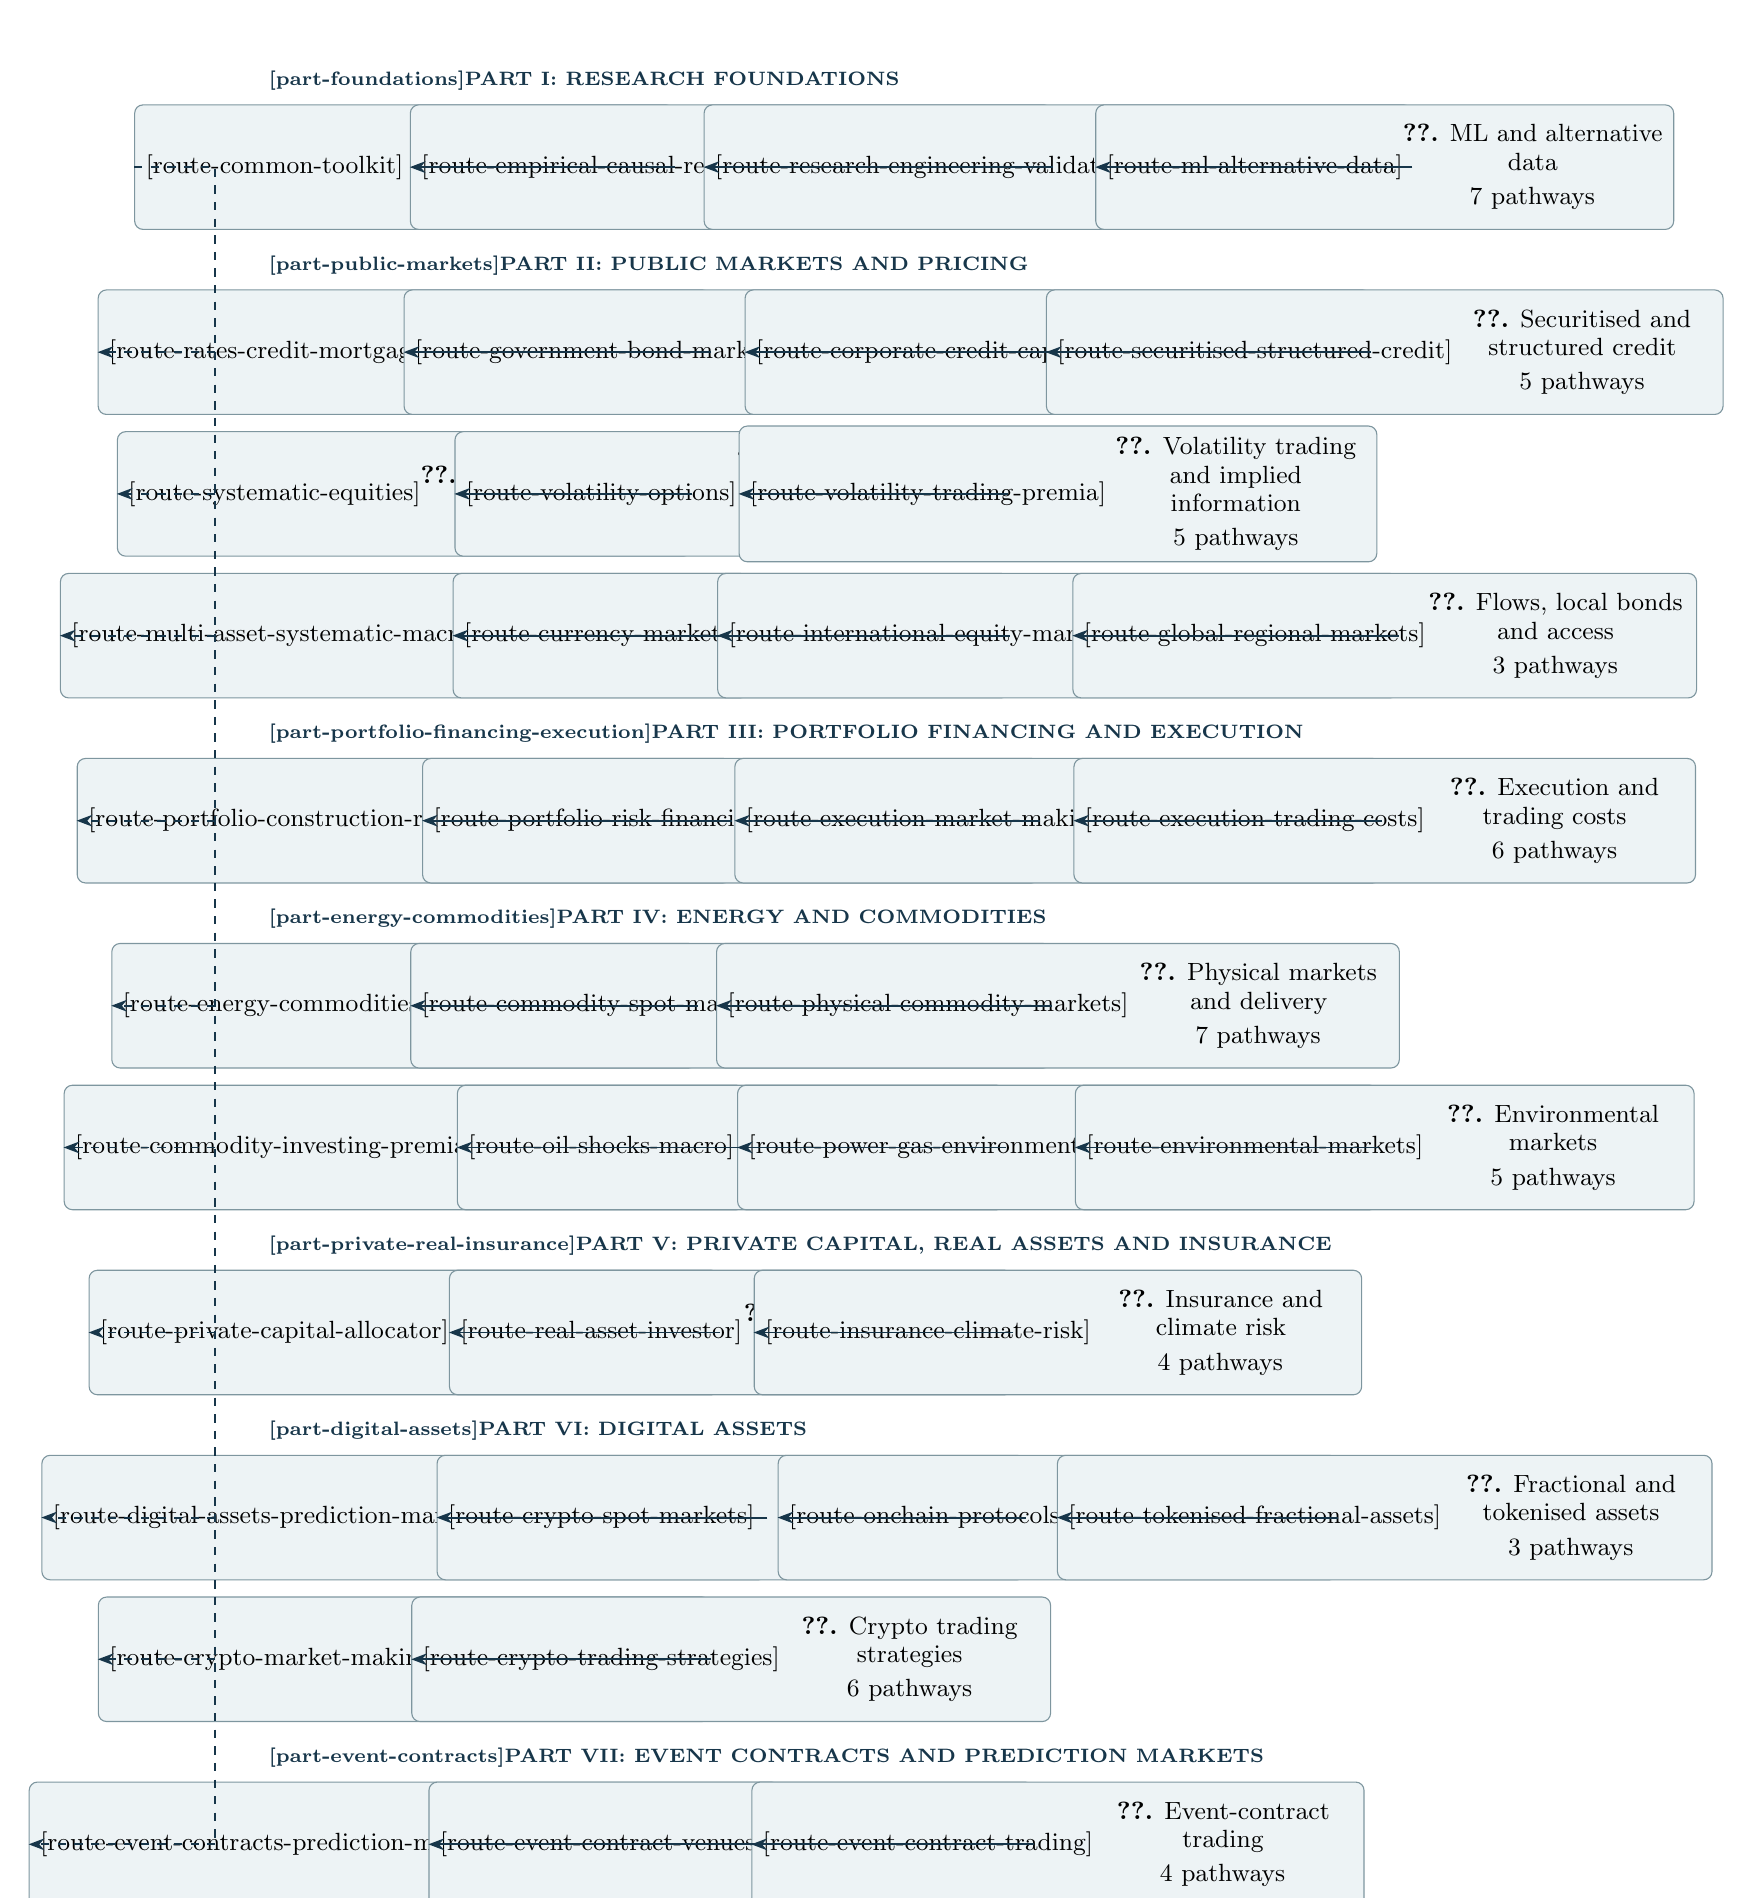
\begin{tikzpicture}[x=1cm,y=1cm]
\node[maplabel,anchor=west] at (-1.80,0.00) {\hyperref[part-foundations]{PART I: RESEARCH FOUNDATIONS}};
\node[pathnode] (common-toolkit) at (0.00,-1.10) {\MeasurePathNode{3.30cm}{\textbf{\ref*{route-common-toolkit}.} Common toolkit\\[2pt]{\small 6 pathways}}\hyperref[route-common-toolkit]{\parbox[c][\pathnodeheight][c]{3.30cm}{\centering \textbf{\ref*{route-common-toolkit}.} Common toolkit\\[2pt]{\small 6 pathways}}}};
\node[pathnode] (empirical-causal-research) at (4.15,-1.10) {\MeasurePathNode{3.30cm}{\textbf{\ref*{route-empirical-causal-research}.} Empirical and causal research\\[2pt]{\small 7 pathways}}\hyperref[route-empirical-causal-research]{\parbox[c][\pathnodeheight][c]{3.30cm}{\centering \textbf{\ref*{route-empirical-causal-research}.} Empirical and causal research\\[2pt]{\small 7 pathways}}}};
\node[pathnode] (research-engineering-validation) at (8.30,-1.10) {\MeasurePathNode{3.30cm}{\textbf{\ref*{route-research-engineering-validation}.} Research engineering\\[2pt]{\small 4 pathways}}\hyperref[route-research-engineering-validation]{\parbox[c][\pathnodeheight][c]{3.30cm}{\centering \textbf{\ref*{route-research-engineering-validation}.} Research engineering\\[2pt]{\small 4 pathways}}}};
\node[pathnode] (ml-alternative-data) at (12.45,-1.10) {\MeasurePathNode{3.30cm}{\textbf{\ref*{route-ml-alternative-data}.} ML and alternative data\\[2pt]{\small 7 pathways}}\hyperref[route-ml-alternative-data]{\parbox[c][\pathnodeheight][c]{3.30cm}{\centering \textbf{\ref*{route-ml-alternative-data}.} ML and alternative data\\[2pt]{\small 7 pathways}}}};
\draw[patharrow] (common-toolkit.east) -- (empirical-causal-research.west);
\draw[patharrow] (empirical-causal-research.east) -- (research-engineering-validation.west);
\draw[patharrow] (research-engineering-validation.east) -- (ml-alternative-data.west);
\node[maplabel,anchor=west] at (-1.80,-2.35) {\hyperref[part-public-markets]{PART II: PUBLIC MARKETS AND PRICING}};
\node[pathnode] (rates-credit-mortgages) at (0.00,-3.45) {\MeasurePathNode{3.30cm}{\textbf{\ref*{route-rates-credit-mortgages}.} Rates: curves, premia and derivatives\\[2pt]{\small 5 pathways}}\hyperref[route-rates-credit-mortgages]{\parbox[c][\pathnodeheight][c]{3.30cm}{\centering \textbf{\ref*{route-rates-credit-mortgages}.} Rates: curves, premia and derivatives\\[2pt]{\small 5 pathways}}}};
\node[pathnode] (government-bond-markets) at (4.15,-3.45) {\MeasurePathNode{3.30cm}{\textbf{\ref*{route-government-bond-markets}.} Government bonds and sovereign debt\\[2pt]{\small 5 pathways}}\hyperref[route-government-bond-markets]{\parbox[c][\pathnodeheight][c]{3.30cm}{\centering \textbf{\ref*{route-government-bond-markets}.} Government bonds and sovereign debt\\[2pt]{\small 5 pathways}}}};
\node[pathnode] (corporate-credit-capital) at (8.30,-3.45) {\MeasurePathNode{3.30cm}{\textbf{\ref*{route-corporate-credit-capital}.} Credit, hybrids and labelled bonds\\[2pt]{\small 5 pathways}}\hyperref[route-corporate-credit-capital]{\parbox[c][\pathnodeheight][c]{3.30cm}{\centering \textbf{\ref*{route-corporate-credit-capital}.} Credit, hybrids and labelled bonds\\[2pt]{\small 5 pathways}}}};
\node[pathnode] (securitised-structured-credit) at (12.45,-3.45) {\MeasurePathNode{3.30cm}{\textbf{\ref*{route-securitised-structured-credit}.} Securitised and structured credit\\[2pt]{\small 5 pathways}}\hyperref[route-securitised-structured-credit]{\parbox[c][\pathnodeheight][c]{3.30cm}{\centering \textbf{\ref*{route-securitised-structured-credit}.} Securitised and structured credit\\[2pt]{\small 5 pathways}}}};
\draw[patharrow] (rates-credit-mortgages.east) -- (government-bond-markets.west);
\draw[patharrow] (government-bond-markets.east) -- (corporate-credit-capital.west);
\draw[patharrow] (corporate-credit-capital.east) -- (securitised-structured-credit.west);
\node[pathnode] (systematic-equities) at (0.00,-5.25) {\MeasurePathNode{3.30cm}{\textbf{\ref*{route-systematic-equities}.} Systematic equities\\[2pt]{\small 7 pathways}}\hyperref[route-systematic-equities]{\parbox[c][\pathnodeheight][c]{3.30cm}{\centering \textbf{\ref*{route-systematic-equities}.} Systematic equities\\[2pt]{\small 7 pathways}}}};
\node[pathnode] (volatility-options) at (4.15,-5.25) {\MeasurePathNode{3.30cm}{\textbf{\ref*{route-volatility-options}.} Option pricing and hedging\\[2pt]{\small 6 pathways}}\hyperref[route-volatility-options]{\parbox[c][\pathnodeheight][c]{3.30cm}{\centering \textbf{\ref*{route-volatility-options}.} Option pricing and hedging\\[2pt]{\small 6 pathways}}}};
\node[pathnode] (volatility-trading-premia) at (8.30,-5.25) {\MeasurePathNode{3.30cm}{\textbf{\ref*{route-volatility-trading-premia}.} Volatility trading and implied information\\[2pt]{\small 5 pathways}}\hyperref[route-volatility-trading-premia]{\parbox[c][\pathnodeheight][c]{3.30cm}{\centering \textbf{\ref*{route-volatility-trading-premia}.} Volatility trading and implied information\\[2pt]{\small 5 pathways}}}};
\draw[patharrow] (systematic-equities.east) -- (volatility-options.west);
\draw[patharrow] (volatility-options.east) -- (volatility-trading-premia.west);
\node[pathnode] (multi-asset-systematic-macro) at (0.00,-7.05) {\MeasurePathNode{3.30cm}{\textbf{\ref*{route-multi-asset-systematic-macro}.} Multi-asset and macro\\[2pt]{\small 6 pathways}}\hyperref[route-multi-asset-systematic-macro]{\parbox[c][\pathnodeheight][c]{3.30cm}{\centering \textbf{\ref*{route-multi-asset-systematic-macro}.} Multi-asset and macro\\[2pt]{\small 6 pathways}}}};
\node[pathnode] (currency-markets) at (4.15,-7.05) {\MeasurePathNode{3.30cm}{\textbf{\ref*{route-currency-markets}.} Currency markets\\[2pt]{\small 7 pathways}}\hyperref[route-currency-markets]{\parbox[c][\pathnodeheight][c]{3.30cm}{\centering \textbf{\ref*{route-currency-markets}.} Currency markets\\[2pt]{\small 7 pathways}}}};
\node[pathnode] (international-equity-markets) at (8.30,-7.05) {\MeasurePathNode{3.30cm}{\textbf{\ref*{route-international-equity-markets}.} International equity markets\\[2pt]{\small 5 pathways}}\hyperref[route-international-equity-markets]{\parbox[c][\pathnodeheight][c]{3.30cm}{\centering \textbf{\ref*{route-international-equity-markets}.} International equity markets\\[2pt]{\small 5 pathways}}}};
\node[pathnode] (global-regional-markets) at (12.45,-7.05) {\MeasurePathNode{3.30cm}{\textbf{\ref*{route-global-regional-markets}.} Flows, local bonds and access\\[2pt]{\small 3 pathways}}\hyperref[route-global-regional-markets]{\parbox[c][\pathnodeheight][c]{3.30cm}{\centering \textbf{\ref*{route-global-regional-markets}.} Flows, local bonds and access\\[2pt]{\small 3 pathways}}}};
\draw[patharrow] (multi-asset-systematic-macro.east) -- (currency-markets.west);
\draw[patharrow] (currency-markets.east) -- (international-equity-markets.west);
\draw[patharrow] (international-equity-markets.east) -- (global-regional-markets.west);
\node[maplabel,anchor=west] at (-1.80,-8.30) {\hyperref[part-portfolio-financing-execution]{PART III: PORTFOLIO FINANCING AND EXECUTION}};
\node[pathnode] (portfolio-construction-risk) at (0.00,-9.40) {\MeasurePathNode{3.30cm}{\textbf{\ref*{route-portfolio-construction-risk}.} Portfolio construction and risk\\[2pt]{\small 4 pathways}}\hyperref[route-portfolio-construction-risk]{\parbox[c][\pathnodeheight][c]{3.30cm}{\centering \textbf{\ref*{route-portfolio-construction-risk}.} Portfolio construction and risk\\[2pt]{\small 4 pathways}}}};
\node[pathnode] (portfolio-risk-financing) at (4.15,-9.40) {\MeasurePathNode{3.30cm}{\textbf{\ref*{route-portfolio-risk-financing}.} Funding, collateral and liquidity\\[2pt]{\small 5 pathways}}\hyperref[route-portfolio-risk-financing]{\parbox[c][\pathnodeheight][c]{3.30cm}{\centering \textbf{\ref*{route-portfolio-risk-financing}.} Funding, collateral and liquidity\\[2pt]{\small 5 pathways}}}};
\node[pathnode] (execution-market-making) at (8.30,-9.40) {\MeasurePathNode{3.30cm}{\textbf{\ref*{route-execution-market-making}.} Microstructure and market making\\[2pt]{\small 7 pathways}}\hyperref[route-execution-market-making]{\parbox[c][\pathnodeheight][c]{3.30cm}{\centering \textbf{\ref*{route-execution-market-making}.} Microstructure and market making\\[2pt]{\small 7 pathways}}}};
\node[pathnode] (execution-trading-costs) at (12.45,-9.40) {\MeasurePathNode{3.30cm}{\textbf{\ref*{route-execution-trading-costs}.} Execution and trading costs\\[2pt]{\small 6 pathways}}\hyperref[route-execution-trading-costs]{\parbox[c][\pathnodeheight][c]{3.30cm}{\centering \textbf{\ref*{route-execution-trading-costs}.} Execution and trading costs\\[2pt]{\small 6 pathways}}}};
\draw[patharrow] (portfolio-construction-risk.east) -- (portfolio-risk-financing.west);
\draw[patharrow] (portfolio-risk-financing.east) -- (execution-market-making.west);
\draw[patharrow] (execution-market-making.east) -- (execution-trading-costs.west);
\node[maplabel,anchor=west] at (-1.80,-10.65) {\hyperref[part-energy-commodities]{PART IV: ENERGY AND COMMODITIES}};
\node[pathnode] (energy-commodities) at (0.00,-11.75) {\MeasurePathNode{3.30cm}{\textbf{\ref*{route-energy-commodities}.} Commodity futures and curves\\[2pt]{\small 4 pathways}}\hyperref[route-energy-commodities]{\parbox[c][\pathnodeheight][c]{3.30cm}{\centering \textbf{\ref*{route-energy-commodities}.} Commodity futures and curves\\[2pt]{\small 4 pathways}}}};
\node[pathnode] (commodity-spot-markets) at (4.15,-11.75) {\MeasurePathNode{3.30cm}{\textbf{\ref*{route-commodity-spot-markets}.} Spot markets and prices\\[2pt]{\small 5 pathways}}\hyperref[route-commodity-spot-markets]{\parbox[c][\pathnodeheight][c]{3.30cm}{\centering \textbf{\ref*{route-commodity-spot-markets}.} Spot markets and prices\\[2pt]{\small 5 pathways}}}};
\node[pathnode] (physical-commodity-markets) at (8.30,-11.75) {\MeasurePathNode{3.30cm}{\textbf{\ref*{route-physical-commodity-markets}.} Physical markets and delivery\\[2pt]{\small 7 pathways}}\hyperref[route-physical-commodity-markets]{\parbox[c][\pathnodeheight][c]{3.30cm}{\centering \textbf{\ref*{route-physical-commodity-markets}.} Physical markets and delivery\\[2pt]{\small 7 pathways}}}};
\draw[patharrow] (energy-commodities.east) -- (commodity-spot-markets.west);
\draw[patharrow] (commodity-spot-markets.east) -- (physical-commodity-markets.west);
\node[pathnode] (commodity-investing-premia) at (0.00,-13.55) {\MeasurePathNode{3.30cm}{\textbf{\ref*{route-commodity-investing-premia}.} Commodity premia and investing\\[2pt]{\small 5 pathways}}\hyperref[route-commodity-investing-premia]{\parbox[c][\pathnodeheight][c]{3.30cm}{\centering \textbf{\ref*{route-commodity-investing-premia}.} Commodity premia and investing\\[2pt]{\small 5 pathways}}}};
\node[pathnode] (oil-shocks-macro) at (4.15,-13.55) {\MeasurePathNode{3.30cm}{\textbf{\ref*{route-oil-shocks-macro}.} Oil shocks and forecasting\\[2pt]{\small 4 pathways}}\hyperref[route-oil-shocks-macro]{\parbox[c][\pathnodeheight][c]{3.30cm}{\centering \textbf{\ref*{route-oil-shocks-macro}.} Oil shocks and forecasting\\[2pt]{\small 4 pathways}}}};
\node[pathnode] (power-gas-environmental) at (8.30,-13.55) {\MeasurePathNode{3.30cm}{\textbf{\ref*{route-power-gas-environmental}.} Gas and power markets\\[2pt]{\small 7 pathways}}\hyperref[route-power-gas-environmental]{\parbox[c][\pathnodeheight][c]{3.30cm}{\centering \textbf{\ref*{route-power-gas-environmental}.} Gas and power markets\\[2pt]{\small 7 pathways}}}};
\node[pathnode] (environmental-markets) at (12.45,-13.55) {\MeasurePathNode{3.30cm}{\textbf{\ref*{route-environmental-markets}.} Environmental markets\\[2pt]{\small 5 pathways}}\hyperref[route-environmental-markets]{\parbox[c][\pathnodeheight][c]{3.30cm}{\centering \textbf{\ref*{route-environmental-markets}.} Environmental markets\\[2pt]{\small 5 pathways}}}};
\draw[patharrow] (commodity-investing-premia.east) -- (oil-shocks-macro.west);
\draw[patharrow] (oil-shocks-macro.east) -- (power-gas-environmental.west);
\draw[patharrow] (power-gas-environmental.east) -- (environmental-markets.west);
\node[maplabel,anchor=west] at (-1.80,-14.80) {\hyperref[part-private-real-insurance]{PART V: PRIVATE CAPITAL, REAL ASSETS AND INSURANCE}};
\node[pathnode] (private-capital-allocator) at (0.00,-15.90) {\MeasurePathNode{3.30cm}{\textbf{\ref*{route-private-capital-allocator}.} Private-capital allocator\\[2pt]{\small 7 pathways}}\hyperref[route-private-capital-allocator]{\parbox[c][\pathnodeheight][c]{3.30cm}{\centering \textbf{\ref*{route-private-capital-allocator}.} Private-capital allocator\\[2pt]{\small 7 pathways}}}};
\node[pathnode] (real-asset-investor) at (4.15,-15.90) {\MeasurePathNode{3.30cm}{\textbf{\ref*{route-real-asset-investor}.} Real-asset investor\\[2pt]{\small 5 pathways}}\hyperref[route-real-asset-investor]{\parbox[c][\pathnodeheight][c]{3.30cm}{\centering \textbf{\ref*{route-real-asset-investor}.} Real-asset investor\\[2pt]{\small 5 pathways}}}};
\node[pathnode] (insurance-climate-risk) at (8.30,-15.90) {\MeasurePathNode{3.30cm}{\textbf{\ref*{route-insurance-climate-risk}.} Insurance and climate risk\\[2pt]{\small 4 pathways}}\hyperref[route-insurance-climate-risk]{\parbox[c][\pathnodeheight][c]{3.30cm}{\centering \textbf{\ref*{route-insurance-climate-risk}.} Insurance and climate risk\\[2pt]{\small 4 pathways}}}};
\draw[patharrow] (private-capital-allocator.east) -- (real-asset-investor.west);
\draw[patharrow] (real-asset-investor.east) -- (insurance-climate-risk.west);
\node[maplabel,anchor=west] at (-1.80,-17.15) {\hyperref[part-digital-assets]{PART VI: DIGITAL ASSETS}};
\node[pathnode] (digital-assets-prediction-markets) at (0.00,-18.25) {\MeasurePathNode{3.30cm}{\textbf{\ref*{route-digital-assets-prediction-markets}.} Crypto venues and derivatives\\[2pt]{\small 6 pathways}}\hyperref[route-digital-assets-prediction-markets]{\parbox[c][\pathnodeheight][c]{3.30cm}{\centering \textbf{\ref*{route-digital-assets-prediction-markets}.} Crypto venues and derivatives\\[2pt]{\small 6 pathways}}}};
\node[pathnode] (crypto-spot-markets) at (4.15,-18.25) {\MeasurePathNode{3.30cm}{\textbf{\ref*{route-crypto-spot-markets}.} Crypto spot markets\\[2pt]{\small 6 pathways}}\hyperref[route-crypto-spot-markets]{\parbox[c][\pathnodeheight][c]{3.30cm}{\centering \textbf{\ref*{route-crypto-spot-markets}.} Crypto spot markets\\[2pt]{\small 6 pathways}}}};
\node[pathnode] (onchain-protocols) at (8.30,-18.25) {\MeasurePathNode{3.30cm}{\textbf{\ref*{route-onchain-protocols}.} On-chain protocols\\[2pt]{\small 7 pathways}}\hyperref[route-onchain-protocols]{\parbox[c][\pathnodeheight][c]{3.30cm}{\centering \textbf{\ref*{route-onchain-protocols}.} On-chain protocols\\[2pt]{\small 7 pathways}}}};
\node[pathnode] (tokenised-fractional-assets) at (12.45,-18.25) {\MeasurePathNode{3.30cm}{\textbf{\ref*{route-tokenised-fractional-assets}.} Fractional and tokenised assets\\[2pt]{\small 3 pathways}}\hyperref[route-tokenised-fractional-assets]{\parbox[c][\pathnodeheight][c]{3.30cm}{\centering \textbf{\ref*{route-tokenised-fractional-assets}.} Fractional and tokenised assets\\[2pt]{\small 3 pathways}}}};
\draw[patharrow] (digital-assets-prediction-markets.east) -- (crypto-spot-markets.west);
\draw[patharrow] (crypto-spot-markets.east) -- (onchain-protocols.west);
\draw[patharrow] (onchain-protocols.east) -- (tokenised-fractional-assets.west);
\node[pathnode] (crypto-market-making) at (0.00,-20.05) {\MeasurePathNode{3.30cm}{\textbf{\ref*{route-crypto-market-making}.} Crypto market making\\[2pt]{\small 5 pathways}}\hyperref[route-crypto-market-making]{\parbox[c][\pathnodeheight][c]{3.30cm}{\centering \textbf{\ref*{route-crypto-market-making}.} Crypto market making\\[2pt]{\small 5 pathways}}}};
\node[pathnode] (crypto-trading-strategies) at (4.15,-20.05) {\MeasurePathNode{3.30cm}{\textbf{\ref*{route-crypto-trading-strategies}.} Crypto trading strategies\\[2pt]{\small 6 pathways}}\hyperref[route-crypto-trading-strategies]{\parbox[c][\pathnodeheight][c]{3.30cm}{\centering \textbf{\ref*{route-crypto-trading-strategies}.} Crypto trading strategies\\[2pt]{\small 6 pathways}}}};
\draw[patharrow] (crypto-market-making.east) -- (crypto-trading-strategies.west);
\node[maplabel,anchor=west] at (-1.80,-21.30) {\hyperref[part-event-contracts]{PART VII: EVENT CONTRACTS AND PREDICTION MARKETS}};
\node[pathnode] (event-contracts-prediction-markets) at (0.00,-22.40) {\MeasurePathNode{3.30cm}{\textbf{\ref*{route-event-contracts-prediction-markets}.} Event contracts and prediction markets\\[2pt]{\small 4 pathways}}\hyperref[route-event-contracts-prediction-markets]{\parbox[c][\pathnodeheight][c]{3.30cm}{\centering \textbf{\ref*{route-event-contracts-prediction-markets}.} Event contracts and prediction markets\\[2pt]{\small 4 pathways}}}};
\node[pathnode] (event-contract-venues) at (4.15,-22.40) {\MeasurePathNode{3.30cm}{\textbf{\ref*{route-event-contract-venues}.} Venues, settlement and regulation\\[2pt]{\small 4 pathways}}\hyperref[route-event-contract-venues]{\parbox[c][\pathnodeheight][c]{3.30cm}{\centering \textbf{\ref*{route-event-contract-venues}.} Venues, settlement and regulation\\[2pt]{\small 4 pathways}}}};
\node[pathnode] (event-contract-trading) at (8.30,-22.40) {\MeasurePathNode{3.30cm}{\textbf{\ref*{route-event-contract-trading}.} Event-contract trading\\[2pt]{\small 4 pathways}}\hyperref[route-event-contract-trading]{\parbox[c][\pathnodeheight][c]{3.30cm}{\centering \textbf{\ref*{route-event-contract-trading}.} Event-contract trading\\[2pt]{\small 4 pathways}}}};
\draw[patharrow] (event-contracts-prediction-markets.east) -- (event-contract-venues.west);
\draw[patharrow] (event-contract-venues.east) -- (event-contract-trading.west);
\draw[entryline] (common-toolkit.west) -- (-2.40,-1.10) -- (-2.40,-22.40);
\draw[entryarrow] (-2.40,-3.45) -- (rates-credit-mortgages.west);
\draw[entryarrow] (-2.40,-5.25) -- (systematic-equities.west);
\draw[entryarrow] (-2.40,-7.05) -- (multi-asset-systematic-macro.west);
\draw[entryarrow] (-2.40,-9.40) -- (portfolio-construction-risk.west);
\draw[entryarrow] (-2.40,-11.75) -- (energy-commodities.west);
\draw[entryarrow] (-2.40,-13.55) -- (commodity-investing-premia.west);
\draw[entryarrow] (-2.40,-15.90) -- (private-capital-allocator.west);
\draw[entryarrow] (-2.40,-18.25) -- (digital-assets-prediction-markets.west);
\draw[entryarrow] (-2.40,-20.05) -- (crypto-market-making.west);
\draw[entryarrow] (-2.40,-22.40) -- (event-contracts-prediction-markets.west);
\end{tikzpicture}
\end{center}
\clearpage
\part{Research foundations}\label{part-foundations}
Build a common quantitative toolkit with probability, inference and Bayesian methods; empirical and causal research design with correct standard errors, event studies and experiments; a reproducible research process; and sound model and data evaluation.

\textbf{Sections in learning order}\begin{enumerate}
\item[\ref*{route-common-toolkit}.] \hyperref[route-common-toolkit]{Common toolkit} --- Establish probability, inference, data timing and portfolio decision basics; then deepen probability and econometric theory, continuous-time, high-dimensional and time-series methods. Bayesian methods build on statistical inference, and numerical methods on stochastic calculus.
\item[\ref*{route-empirical-causal-research}.] \hyperref[route-empirical-causal-research]{Empirical asset pricing and causal inference} --- Get standard errors right first; then test return evidence against asset-pricing restrictions and replication standards, forecast returns and measure event effects, and identify the effects of actions with credible causal designs and controlled experiments.
\item[\ref*{route-research-engineering-validation}.] \hyperref[route-research-engineering-validation]{Research engineering and validation} --- Make data availability, research records, code and trading events auditable and reproducible before assessing model evidence.
\item[\ref*{route-ml-alternative-data}.] \hyperref[route-ml-alternative-data]{ML and alternative data} --- Start with statistical learning and time-series validation (4.1): return prediction, financial-ML evaluation, deep forecasting and reinforcement learning build on it, and text and alternative data build on the evaluation pathway (4.3). The overview checkpoint closes the section after 4.1 and 4.3.
\end{enumerate}
\hyperref[learning-map]{Return to the learning pathway DAG.}
\clearpage
\section{Common toolkit}\label{route-common-toolkit}
\label{route-1}
\textbf{Learning sequence.} Establish probability, inference, data timing and portfolio decision basics; then deepen probability and econometric theory, continuous-time, high-dimensional and time-series methods. Bayesian methods build on statistical inference, and numerical methods on stochastic calculus.

\textbf{Section goals.} Across its pathways, this section teaches you to:
\begin{itemize}[leftmargin=1.4em,itemsep=0pt,topsep=1pt]
\item derive the sampling distribution, test and asymptotic or bootstrap approximation behind an estimator (\hyperref[specialist-probability-statistical-inference]{\ref*{specialist-probability-statistical-inference}})
\item derive hedging and allocation rules from continuous-time models and the control problems they solve (\hyperref[specialist-stochastic-calculus-control]{\ref*{specialist-stochastic-calculus-control}})
\item estimate large covariance and factor structures and test tail and dependence assumptions (\hyperref[specialist-high-dimensional-estimation]{\ref*{specialist-high-dimensional-estimation}})
\item build and evaluate time-series, volatility and regime models (\hyperref[specialist-time-series-volatility]{\ref*{specialist-time-series-volatility}})
\item carry parameter uncertainty into portfolio and model-selection decisions with Bayesian methods and shrinkage (\hyperref[specialist-bayesian-parameter-uncertainty]{\ref*{specialist-bayesian-parameter-uncertainty}})
\item choose and validate numerical methods for pricing and portfolios (\hyperref[specialist-numerical-methods-optimisation]{\ref*{specialist-numerical-methods-optimisation}})
\end{itemize}
\textbf{Overview outcome.} Write a reproducible research record for a simple signal: decision-time data, an economic mechanism, the uncertainty of the headline estimate, a portfolio decision and the evidence that would reject it.

\textbf{Prerequisites.} Calculus, linear algebra and the ability to inspect and transform tabular time-series data.

\textbf{Required readings, in order}
\begin{enumerate}\raggedright
\Needspace{5\baselineskip}\item \href{institutional_quantitative_finance_reading_list.pdf\#prob-wasserman}{Larry Wasserman, \emph{All of Statistics: A Concise Course in Statistical Inference}}\CataloguePage{9}\NoteKey{prob-wasserman}\par Build a compact base in probability, estimation and testing before interpreting a backtest.
\Needspace{5\baselineskip}\item \href{institutional_quantitative_finance_reading_list.pdf\#s15-campbell}{John Y. Campbell, Andrew W. Lo and A. Craig MacKinlay, \emph{The Econometrics of Financial Markets}}\CataloguePage{35}\NoteKey{s15-campbell}\par Connect financial time-series and cross-sectional evidence to the econometric assumptions behind it.
\Needspace{5\baselineskip}\item \href{institutional_quantitative_finance_reading_list.pdf\#s6-cochrane}{John H. Cochrane, \emph{Asset Pricing}, revised edition}\CataloguePage{27}\NoteKey{s6-cochrane}\par Use asset-pricing restrictions to ask which risks or cash flows could explain a return pattern.
\Needspace{5\baselineskip}\item \href{institutional_quantitative_finance_reading_list.pdf\#alpha-boyd}{Stephen Boyd and Lieven Vandenberghe, \emph{Convex Optimization}}\CataloguePage{23}\NoteKey{alpha-boyd}\par\emph{Selection:} Duality and sensitivity analysis chapters (topic selection; numbering depends on the copy).\par Express a portfolio choice as an objective with explicit constraints rather than a weight heuristic.
\Needspace{5\baselineskip}\item \href{institutional_quantitative_finance_reading_list.pdf\#s7-meucci}{Attilio Meucci, \emph{Risk and Asset Allocation}}\CataloguePage{106}\NoteKey{s7-meucci}\par Translate estimates into exposure, dependence and portfolio risk under imperfect inputs.
\Needspace{5\baselineskip}\item \href{institutional_quantitative_finance_reading_list.pdf\#s6-pbo}{David H. Bailey et al., ``The Probability of Backtest Overfitting''}\CataloguePage{82}\NoteKey{s6-pbo}\par Account for the number of strategies tried before treating the selected result as evidence.
\Needspace{5\baselineskip}\item \href{institutional_quantitative_finance_reading_list.pdf\#s8-bitemporal}{Martin Fowler, \emph{Bitemporal History} (2021)}\CataloguePage{531}\NoteKey{s8-bitemporal}\par Separate the date a fact describes from the date it became available to the researcher.
\end{enumerate}
\Needspace{5\baselineskip}\textbf{Checkpoint.} Write a one-page research record for a simple public-data signal: identify the decision timestamp, data vintages, candidate family, economic hypothesis, estimation window, the uncertainty of the headline estimate, risk limits and the evidence that would reject it. Rebuild the same result from the recorded inputs.

\textbf{Optional branches.} \href{institutional_quantitative_finance_reading_list.pdf\#section.1.1}{Deepen probability, inference or stochastic-process prerequisites as needed.}\BranchPage{9} \href{institutional_quantitative_finance_reading_list.pdf\#prob-course-ucsd-math280}{Use the identified full-year graduate probability video and slide archive when a structured course is helpful.}\BranchPage{543} \href{institutional_quantitative_finance_reading_list.pdf\#latest-follmer-schied}{Deepen discrete-time arbitrage, incomplete-market hedging and risk-measure foundations with the 2025 fifth edition.}\BranchPage{20} \href{institutional_quantitative_finance_reading_list.pdf\#wide-efron-hastie-casi}{Bridge classical inference to bootstrap, FDR and lasso.}\BranchPage{13}
\par\textbf{Continue in this section.} \hyperref[specialist-probability-statistical-inference]{Probability, statistical inference and econometric theory}; \hyperref[specialist-stochastic-calculus-control]{Stochastic calculus and continuous-time control}; \hyperref[specialist-high-dimensional-estimation]{High-dimensional estimation, random matrices and heavy tails}; \hyperref[specialist-time-series-volatility]{Time-series econometrics and volatility forecasting}; \hyperref[specialist-bayesian-parameter-uncertainty]{Bayesian inference, shrinkage and parameter uncertainty}; \hyperref[specialist-numerical-methods-optimisation]{Optimisation and numerical methods for pricing and portfolios}.
\par{\small \hyperref[learning-map]{Learning pathway DAG} \textbar{} \hyperref[map-common-toolkit]{Section DAG}\NoteKey{common-toolkit}}
\clearpage
\subsection*{Common toolkit: pathway DAG}\phantomsection\label{map-common-toolkit}
\addcontentsline{toc}{subsection}{Common toolkit: pathway DAG}
Start with the section overview's readings, for orientation. Solid arrows show prerequisites within this section. Dashed connectors identify entry points with no further prerequisite in this section; the linked foundations below still apply. Follow the arrows for dependencies and the subsection numbers for reading order. Every node is clickable.
\begin{center}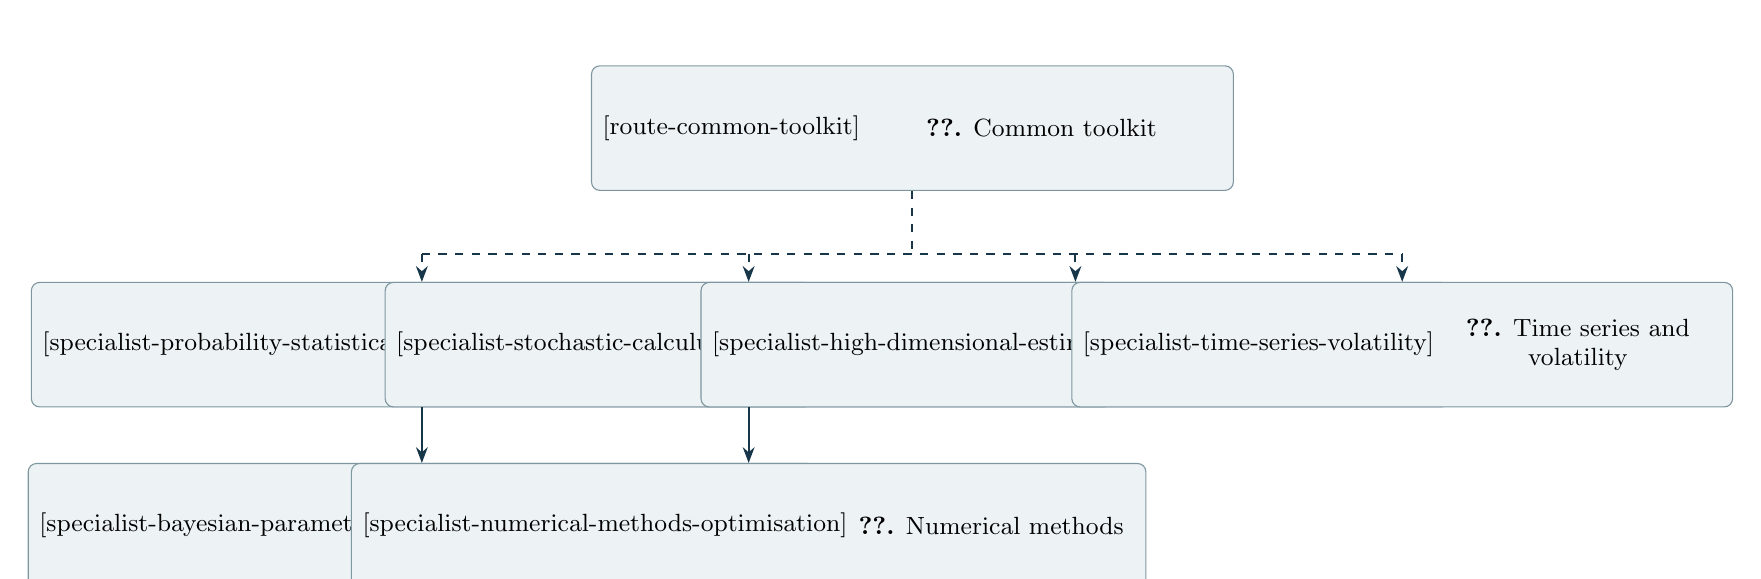
\begin{tikzpicture}[x=1cm,y=1cm]
\node[pathnode] (common-toolkit) at (6.23,0) {\MeasurePathNode{4.6cm}{\textbf{\ref*{route-common-toolkit}.} Common toolkit}\hyperref[route-common-toolkit]{\parbox[c][\pathnodeheight][c]{4.6cm}{\centering \textbf{\ref*{route-common-toolkit}.} Common toolkit}}};
\node[pathnode] (probability-statistical-inference) at (0.00,-2.75) {\MeasurePathNode{3.65cm}{\textbf{\ref*{specialist-probability-statistical-inference}.} Probability and inference}\hyperref[specialist-probability-statistical-inference]{\parbox[c][\pathnodeheight][c]{3.65cm}{\centering \textbf{\ref*{specialist-probability-statistical-inference}.} Probability and inference}}};
\node[pathnode] (stochastic-calculus-control) at (4.15,-2.75) {\MeasurePathNode{3.65cm}{\textbf{\ref*{specialist-stochastic-calculus-control}.} Stochastic calculus and control}\hyperref[specialist-stochastic-calculus-control]{\parbox[c][\pathnodeheight][c]{3.65cm}{\centering \textbf{\ref*{specialist-stochastic-calculus-control}.} Stochastic calculus and control}}};
\node[pathnode] (high-dimensional-estimation) at (8.30,-2.75) {\MeasurePathNode{3.65cm}{\textbf{\ref*{specialist-high-dimensional-estimation}.} High-dimensional estimation}\hyperref[specialist-high-dimensional-estimation]{\parbox[c][\pathnodeheight][c]{3.65cm}{\centering \textbf{\ref*{specialist-high-dimensional-estimation}.} High-dimensional estimation}}};
\node[pathnode] (time-series-volatility) at (12.45,-2.75) {\MeasurePathNode{3.65cm}{\textbf{\ref*{specialist-time-series-volatility}.} Time series and volatility}\hyperref[specialist-time-series-volatility]{\parbox[c][\pathnodeheight][c]{3.65cm}{\centering \textbf{\ref*{specialist-time-series-volatility}.} Time series and volatility}}};
\node[pathnode] (bayesian-parameter-uncertainty) at (0.00,-5.05) {\MeasurePathNode{3.65cm}{\textbf{\ref*{specialist-bayesian-parameter-uncertainty}.} Bayesian methods}\hyperref[specialist-bayesian-parameter-uncertainty]{\parbox[c][\pathnodeheight][c]{3.65cm}{\centering \textbf{\ref*{specialist-bayesian-parameter-uncertainty}.} Bayesian methods}}};
\node[pathnode] (numerical-methods-optimisation) at (4.15,-5.05) {\MeasurePathNode{3.65cm}{\textbf{\ref*{specialist-numerical-methods-optimisation}.} Numerical methods}\hyperref[specialist-numerical-methods-optimisation]{\parbox[c][\pathnodeheight][c]{3.65cm}{\centering \textbf{\ref*{specialist-numerical-methods-optimisation}.} Numerical methods}}};
\draw[entryline] (common-toolkit.south) -- (6.23,-1.60);
\draw[entryline] (0.00,-1.60) -- (12.45,-1.60);
\draw[entryarrow] (0.00,-1.60) -- (probability-statistical-inference.north);
\draw[entryarrow] (4.15,-1.60) -- (stochastic-calculus-control.north);
\draw[entryarrow] (8.30,-1.60) -- (high-dimensional-estimation.north);
\draw[entryarrow] (12.45,-1.60) -- (time-series-volatility.north);
\draw[patharrow] (probability-statistical-inference.south) -- (bayesian-parameter-uncertainty.north);
\draw[patharrow] (stochastic-calculus-control.south) -- (numerical-methods-optimisation.north);
\end{tikzpicture}\end{center}
\hyperref[learning-map]{Return to the whole-guide DAG.}
\Needspace{12\baselineskip}
\subsection{Probability, statistical inference and econometric theory}\label{specialist-probability-statistical-inference}
\textbf{Specialist pathway.} In \hyperref[route-common-toolkit]{Common toolkit}.

\textbf{Outcome.} Derive the sampling distribution, test and asymptotic or bootstrap approximation behind an estimator, and state which assumptions each approximation needs.

\textbf{Prerequisites.} Common toolkit; calculus and linear algebra. Stochastic calculus (1.2) and the Bayesian pathway (1.5) build on this one.

\textbf{Review first.} \hyperref[route-common-toolkit]{Common toolkit}.

\textbf{Required readings, in order}
\begin{enumerate}\raggedright
\Needspace{5\baselineskip}\item \href{institutional_quantitative_finance_reading_list.pdf\#w2-grimmett-stirzaker}{Geoffrey Grimmett and David Stirzaker, \emph{Probability and Random Processes}}\CataloguePage{10}\NoteKey{w2-grimmett-stirzaker}\par \textbf{Foundations.} Work through random variables, generating functions, limit theorems and Markov chains with many exercises.
\Needspace{5\baselineskip}\item \href{institutional_quantitative_finance_reading_list.pdf\#prob-casella}{George Casella and Roger L. Berger, \emph{Statistical Inference}, 2nd ed. (2002)}\CataloguePage{9}\NoteKey{prob-casella}\par \textbf{Foundations.} Learn sufficiency, likelihood, point estimation and hypothesis testing at the level assumed by econometrics texts.
\Needspace{5\baselineskip}\item \href{institutional_quantitative_finance_reading_list.pdf\#prob-williams}{David Williams, \emph{Probability with Martingales} (1991)}\CataloguePage{10}\NoteKey{prob-williams}\par \textbf{Foundations.} Learn conditional expectation, filtrations, stopping times and martingales before continuous-time finance.
\Needspace{5\baselineskip}\item \href{institutional_quantitative_finance_reading_list.pdf\#prob-lehmann-romano}{E. L. Lehmann and Joseph P. Romano, \emph{Testing Statistical Hypotheses}, 3rd ed. (2005)}\CataloguePage{12}\NoteKey{prob-lehmann-romano}\par \textbf{Theory.} Study power, optimal tests and asymptotic testing so that a reported p-value has a defined meaning.
\Needspace{5\baselineskip}\item \href{institutional_quantitative_finance_reading_list.pdf\#prob-vdv}{A. W. van der Vaart, \emph{Asymptotic Statistics} (1998)}\CataloguePage{12}\NoteKey{prob-vdv}\par \textbf{Theory.} Use M-estimation, the delta method and asymptotic efficiency to derive standard errors for nonlinear statistics such as Sharpe ratios.
\Needspace{5\baselineskip}\item \href{institutional_quantitative_finance_reading_list.pdf\#wide-efron-tibshirani-bootstrap}{Bradley Efron and Robert J. Tibshirani, \emph{An Introduction to the Bootstrap}}\CataloguePage{13}\NoteKey{wide-efron-tibshirani-bootstrap}\par \textbf{Methods.} Approximate a sampling distribution by resampling when an analytic standard error is unavailable or unreliable.
\Needspace{5\baselineskip}\item \href{institutional_quantitative_finance_reading_list.pdf\#wide-hayashi-econometrics}{Fumio Hayashi, \emph{Econometrics}}\CataloguePage{36}\NoteKey{wide-hayashi-econometrics}\par \textbf{Methods.} Learn GMM, time-series asymptotics and HAC inference with finance examples.
\Needspace{5\baselineskip}\item \href{institutional_quantitative_finance_reading_list.pdf\#wide-hansen-econometrics}{Bruce E. Hansen, \emph{Econometrics}}\CataloguePage{36}\NoteKey{wide-hansen-econometrics}\par \textbf{Methods.} Use a current graduate text for regression, bootstrap, IV, panel and time-series inference.
\end{enumerate}
\Needspace{5\baselineskip}\textbf{Checkpoint.} Simulate a monthly return series with fat tails and volatility clustering. For the Sharpe ratio and an OLS slope, compare the finite-sample distribution with the delta-method normal approximation and with i.i.d. and block bootstrap intervals; report the coverage of nominal 95\% intervals at 60, 120 and 600 months and explain which assumption fails.

\textbf{Optional branches.} \href{institutional_quantitative_finance_reading_list.pdf\#prob-durrett}{Go further into measure-theoretic probability, martingales and Brownian motion.}\BranchPage{11} \href{institutional_quantitative_finance_reading_list.pdf\#prob-billingsley}{Use a classic measure-theoretic probability reference.}\BranchPage{11} \href{institutional_quantitative_finance_reading_list.pdf\#prob-blitzstein}{Revise calculus-based probability with problems and video lectures.}\BranchPage{9} \href{institutional_quantitative_finance_reading_list.pdf\#w2-rice}{Revise mathematical statistics with data-analysis examples.}\BranchPage{10} \href{institutional_quantitative_finance_reading_list.pdf\#prob-ferguson}{Study large-sample theory compactly.}\BranchPage{12} \href{institutional_quantitative_finance_reading_list.pdf\#prob-nonparametric}{Survey nonparametric estimation, smoothing and the bootstrap.}\BranchPage{13} \href{institutional_quantitative_finance_reading_list.pdf\#s15-wooldridge}{Revise applied regression econometrics.}\BranchPage{35}
\par{\small \hyperref[learning-map]{Learning pathway DAG} \textbar{} \hyperref[route-common-toolkit]{Section overview} \textbar{} \hyperref[map-common-toolkit]{Section DAG}\NoteKey{probability-statistical-inference}}
\Needspace{12\baselineskip}
\subsection{Stochastic calculus and continuous-time control}\label{specialist-stochastic-calculus-control}
\textbf{Specialist pathway.} In \hyperref[route-common-toolkit]{Common toolkit}.

\textbf{Outcome.} Derive a hedging or allocation rule from an SDE model, state the dynamic-programming or BSDE problem it solves, and simulate it with a convergent scheme.

\textbf{Prerequisites.} Common toolkit, measure-theoretic probability and ordinary differential equations.

\textbf{Review first.} \hyperref[route-common-toolkit]{Common toolkit}.

\textbf{Required readings, in order}
\begin{enumerate}\raggedright
\Needspace{5\baselineskip}\item \href{institutional_quantitative_finance_reading_list.pdf\#crypto-shreve}{Steven E. Shreve, \emph{Stochastic Calculus for Finance}, Volumes I and II}\CataloguePage{19}\NoteKey{crypto-shreve}\par\emph{Selection:} Volume II core chapters on stochastic calculus and risk-neutral pricing.\par \textbf{Foundations.} Learn Brownian motion, Ito calculus, Girsanov and risk-neutral pricing at the level used by practitioners.
\Needspace{5\baselineskip}\item \href{institutional_quantitative_finance_reading_list.pdf\#wide-steele-stochastic}{J. Michael Steele, \emph{Stochastic Calculus and Financial Applications}}\CataloguePage{20}\NoteKey{wide-steele-stochastic}\par \textbf{Foundations.} Consolidate martingale and Ito arguments with a second, more intuitive treatment.
\Needspace{5\baselineskip}\item \href{institutional_quantitative_finance_reading_list.pdf\#wide-kloeden-platen}{Peter E. Kloeden and Eckhard Platen, \emph{Numerical Solution of Stochastic Differential Equations}}\CataloguePage{20}\NoteKey{wide-kloeden-platen}\par \textbf{Methods.} Discretise SDEs with Euler and Milstein schemes and distinguish strong from weak convergence.
\Needspace{5\baselineskip}\item \href{institutional_quantitative_finance_reading_list.pdf\#wide-merton-1969}{Robert C. Merton, ``Lifetime Portfolio Selection under Uncertainty: The Continuous-Time Case''}\CataloguePage{21}\NoteKey{wide-merton-1969}\par \textbf{Theory.} Solve the benchmark continuous-time portfolio problem by dynamic programming.
\Needspace{5\baselineskip}\item \href{institutional_quantitative_finance_reading_list.pdf\#wide-pham-control}{Huyên Pham, \emph{Continuous-time Stochastic Control and Optimization with Financial Applications}}\CataloguePage{21}\NoteKey{wide-pham-control}\par \textbf{Methods.} Extend to viscosity solutions, optimal stopping and BSDE formulations with finance applications.
\Needspace{5\baselineskip}\item \href{institutional_quantitative_finance_reading_list.pdf\#wide-elkaroui-bsde}{Nicole El Karoui, Shige Peng and Marie Claire Quenez, ``Backward Stochastic Differential Equations in Finance''}\CataloguePage{22}\NoteKey{wide-elkaroui-bsde}\par \textbf{Valuation.} Connect backward SDEs to hedging, recursive utility and nonlinear pricing.
\Needspace{5\baselineskip}\item \href{institutional_quantitative_finance_reading_list.pdf\#wide-cardaliaguet-lehalle-mfg}{Pierre Cardaliaguet and Charles-Albert Lehalle, ``Mean field game of controls and an application to trade crowding''}\CataloguePage{22}\NoteKey{wide-cardaliaguet-lehalle-mfg}\par \textbf{Implementation.} See how many interacting traders turn an execution problem into a mean-field game.
\Needspace{5\baselineskip}\item \href{institutional_quantitative_finance_reading_list.pdf\#w5-legall}{Jean-François Le Gall, \emph{Brownian Motion, Martingales, and Stochastic Calculus}}\CataloguePage{21}\NoteKey{w5-legall}\par \textbf{Foundations.} Consolidate Brownian motion, martingales and Ito calculus in one compact text.
\Needspace{5\baselineskip}\item \href{institutional_quantitative_finance_reading_list.pdf\#w5-yong-zhou}{Jiongmin Yong and Xun Yu Zhou, \emph{Stochastic Controls: Hamiltonian Systems and HJB Equations}}\CataloguePage{22}\NoteKey{w5-yong-zhou}\par \textbf{Methods.} Connect the maximum principle, HJB equations and linear-quadratic control.
\end{enumerate}
\Needspace{5\baselineskip}\textbf{Checkpoint.} Solve the Merton problem analytically and by a discretised dynamic-programming scheme; simulate the optimal wealth process with Euler and Milstein steps at several step sizes and report the weak-error rate. Then state one execution or hedging problem as an HJB equation and as a BSDE, naming the terminal condition and the control.

\textbf{Optional branches.} \href{institutional_quantitative_finance_reading_list.pdf\#wide-fleming-soner}{Use for viscosity-solution theory when an HJB has no classical solution.}\BranchPage{22} \href{institutional_quantitative_finance_reading_list.pdf\#wide-carmona-delarue-mfg}{Go further into mean-field games with common noise.}\BranchPage{22} \href{institutional_quantitative_finance_reading_list.pdf\#section.1.7}{Browse the full stochastic-control section.}\BranchPage{21} \href{institutional_quantitative_finance_reading_list.pdf\#w4-armstrong-gamma-rough}{See gamma hedging justified pathwise with rough paths.}\BranchPage{129} \href{institutional_quantitative_finance_reading_list.pdf\#w5-revuz-yor}{Go deeper on martingales, local times and time changes.}\BranchPage{20} \href{institutional_quantitative_finance_reading_list.pdf\#w5-pardoux-peng}{Read the founding nonlinear BSDE paper.}\BranchPage{23} \href{institutional_quantitative_finance_reading_list.pdf\#w5-lasry-lions}{Read the founding mean-field games paper.}\BranchPage{22} \href{institutional_quantitative_finance_reading_list.pdf\#w5-peskir-shiryaev}{Treat optimal stopping as a free-boundary problem.}\BranchPage{23} \href{institutional_quantitative_finance_reading_list.pdf\#w5-kushner-dupuis}{Solve control problems numerically by Markov-chain approximation.}\BranchPage{23} \href{institutional_quantitative_finance_reading_list.pdf\#w5-karatzas-shreve-mmf}{Use martingale and duality methods for portfolio choice.}\BranchPage{23} \href{institutional_quantitative_finance_reading_list.pdf\#s15-oksendal}{Use an applied introduction to SDEs.}\BranchPage{19} \href{institutional_quantitative_finance_reading_list.pdf\#s6-karatzas}{Consult the standard graduate reference on Brownian motion.}\BranchPage{20}
\par{\small \hyperref[learning-map]{Learning pathway DAG} \textbar{} \hyperref[route-common-toolkit]{Section overview} \textbar{} \hyperref[map-common-toolkit]{Section DAG}\NoteKey{stochastic-calculus-control}}
\Needspace{12\baselineskip}
\subsection{High-dimensional estimation, random matrices and heavy tails}\label{specialist-high-dimensional-estimation}
\textbf{Specialist pathway.} In \hyperref[route-common-toolkit]{Common toolkit}.

\textbf{Outcome.} Estimate large covariance and factor structures with explicit noise control and test whether tail and dependence assumptions hold.

\textbf{Prerequisites.} Probability, linear algebra and regression.

\textbf{Review first.} \hyperref[route-common-toolkit]{Common toolkit}.

\textbf{Required readings, in order}
\begin{enumerate}\raggedright
\Needspace{5\baselineskip}\item \href{institutional_quantitative_finance_reading_list.pdf\#wide-vershynin-hdp}{Roman Vershynin, \emph{High-Dimensional Probability: An Introduction with Applications in Data Science}}\CataloguePage{16}\NoteKey{wide-vershynin-hdp}\par \textbf{Foundations.} Learn concentration and random-matrix tools behind high-dimensional estimation.
\Needspace{5\baselineskip}\item \href{institutional_quantitative_finance_reading_list.pdf\#wide-wainwright-hds}{Martin J. Wainwright, \emph{High-Dimensional Statistics: A Non-Asymptotic Viewpoint}}\CataloguePage{16}\NoteKey{wide-wainwright-hds}\par \textbf{Theory.} Study sparse regression and covariance estimation with non-asymptotic guarantees.
\Needspace{5\baselineskip}\item \href{institutional_quantitative_finance_reading_list.pdf\#wide-laloux-noise-dressing}{Laurent Laloux, Pierre Cizeau, Jean-Philippe Bouchaud and Marc Potters, ``Noise Dressing of Financial Correlation Matrices''}\CataloguePage{16}\NoteKey{wide-laloux-noise-dressing}\par \textbf{Evidence.} See how much of an empirical correlation matrix is noise.
\Needspace{5\baselineskip}\item \href{institutional_quantitative_finance_reading_list.pdf\#wide-bun-bouchaud-potters-cleaning}{Joël Bun, Jean-Philippe Bouchaud and Marc Potters, ``Cleaning large correlation matrices: Tools from Random Matrix Theory''}\CataloguePage{17}\NoteKey{wide-bun-bouchaud-potters-cleaning}\par \textbf{Methods.} Compare eigenvalue clipping, rotationally invariant and nonlinear-shrinkage estimators.
\Needspace{5\baselineskip}\item \href{institutional_quantitative_finance_reading_list.pdf\#s6-honey}{Olivier Ledoit and Michael Wolf, ``Honey, I Shrunk the Sample Covariance Matrix''}\CataloguePage{97}\NoteKey{s6-honey}\par \textbf{Methods.} Apply linear shrinkage as a baseline estimator.
\Needspace{5\baselineskip}\item \href{institutional_quantitative_finance_reading_list.pdf\#catalogue-0140}{Olivier Ledoit and Michael Wolf, ``Analytical Nonlinear Shrinkage of Large-Dimensional Covariance Matrices''}\CataloguePage{96}\NoteKey{catalogue-0140}\par \textbf{Methods.} Apply analytical nonlinear shrinkage.
\Needspace{5\baselineskip}\item \href{institutional_quantitative_finance_reading_list.pdf\#wide-fan-liao-mincheva-poet}{Jianqing Fan, Yuan Liao and Martina Mincheva, ``Large Covariance Estimation by Thresholding Principal Orthogonal Complements''}\CataloguePage{17}\NoteKey{wide-fan-liao-mincheva-poet}\par \textbf{Methods.} Combine a factor model with sparse residual covariance.
\Needspace{5\baselineskip}\item \href{institutional_quantitative_finance_reading_list.pdf\#wide-bai-ng-factors}{Jushan Bai and Serena Ng, ``Determining the Number of Factors in Approximate Factor Models''}\CataloguePage{37}\NoteKey{wide-bai-ng-factors}\par \textbf{Methods.} Choose the number of factors with information criteria.
\Needspace{5\baselineskip}\item \href{institutional_quantitative_finance_reading_list.pdf\#wide-cont-stylized-facts}{Rama Cont, ``Empirical properties of asset returns: stylized facts and statistical issues''}\CataloguePage{18}\NoteKey{wide-cont-stylized-facts}\par \textbf{Evidence.} Check heavy tails, volatility clustering and leverage effects before assuming Gaussian inputs.
\Needspace{5\baselineskip}\item \href{institutional_quantitative_finance_reading_list.pdf\#wide-embrechts-extremal}{Paul Embrechts, Claudia Klüppelberg and Thomas Mikosch, \emph{Modelling Extremal Events for Insurance and Finance}}\CataloguePage{18}\NoteKey{wide-embrechts-extremal}\par \textbf{Methods.} Estimate tail quantiles with peaks-over-threshold methods.
\Needspace{5\baselineskip}\item \href{institutional_quantitative_finance_reading_list.pdf\#wide-joe-copulas}{Harry Joe, \emph{Dependence Modeling with Copulas}}\CataloguePage{18}\NoteKey{wide-joe-copulas}\par \textbf{Methods.} Model tail dependence beyond correlation.
\end{enumerate}
\Needspace{5\baselineskip}\textbf{Checkpoint.} On a large equity universe, compare sample, linear-shrinkage, nonlinear-shrinkage and POET covariance estimators by out-of-sample minimum-variance risk and eigenvalue spectra. Estimate a tail index and expected shortfall with a peaks-over-threshold model and report sensitivity to the threshold.

\textbf{Optional branches.} \href{institutional_quantitative_finance_reading_list.pdf\#wide-potters-bouchaud-rmt}{Go deeper into random-matrix spectra and free probability.}\BranchPage{16} \href{institutional_quantitative_finance_reading_list.pdf\#wide-taleb-fat-tails}{Stress-test moment estimates under fat tails.}\BranchPage{18} \href{institutional_quantitative_finance_reading_list.pdf\#w2-ledoit-wolf-2004}{Read the statistical linear-shrinkage paper.}\BranchPage{17} \href{institutional_quantitative_finance_reading_list.pdf\#w2-mcneil-frey}{Combine GARCH filtering with EVT.}\BranchPage{18} \href{institutional_quantitative_finance_reading_list.pdf\#w2-longin-solnik}{Study extreme correlation in bear markets.}\BranchPage{19} \href{institutional_quantitative_finance_reading_list.pdf\#w4-luger-covariance-testing}{Regularise covariances by multiple testing of correlations.}\BranchPage{98} \href{institutional_quantitative_finance_reading_list.pdf\#w2-bickel-levina}{Regularise covariance matrices by thresholding.}\BranchPage{17} \href{institutional_quantitative_finance_reading_list.pdf\#wide-buhlmann-vandegeer}{Study high-dimensional methods and theory.}\BranchPage{17}
\par{\small \hyperref[learning-map]{Learning pathway DAG} \textbar{} \hyperref[route-common-toolkit]{Section overview} \textbar{} \hyperref[map-common-toolkit]{Section DAG}\NoteKey{high-dimensional-estimation}}
\Needspace{12\baselineskip}
\subsection{Time-series econometrics and volatility forecasting}\label{specialist-time-series-volatility}
\textbf{Specialist pathway.} In \hyperref[route-common-toolkit]{Common toolkit}.

\textbf{Outcome.} Build and evaluate volatility and regime models with proper loss functions, robust inference and break tests.

\textbf{Prerequisites.} Regression, probability and the common toolkit.

\textbf{Review first.} \hyperref[route-common-toolkit]{Common toolkit}.

\textbf{Required readings, in order}
\begin{enumerate}\raggedright
\Needspace{5\baselineskip}\item \href{institutional_quantitative_finance_reading_list.pdf\#s7-hamilton}{\emph{James D. Hamilton, Time Series Analysis}}\CataloguePage{36}\NoteKey{s7-hamilton}\par \textbf{Foundations.} Learn ARMA, VAR, unit roots, cointegration and state-space models.
\Needspace{5\baselineskip}\item \href{institutional_quantitative_finance_reading_list.pdf\#s7-tsay}{\emph{Ruey S. Tsay, Analysis of Financial Time Series}}\CataloguePage{35}\NoteKey{s7-tsay}\par \textbf{Foundations.} Apply time-series models to financial returns.
\Needspace{5\baselineskip}\item \href{institutional_quantitative_finance_reading_list.pdf\#s7-engle}{\emph{Robert F. Engle, ``Autoregressive Conditional Heteroscedasticity with Estimates of the Variance of United Kingdom Inflation'' (1982)}}\CataloguePage{37}\NoteKey{s7-engle}\par \textbf{Theory.} Introduce conditional heteroskedasticity.
\Needspace{5\baselineskip}\item \href{institutional_quantitative_finance_reading_list.pdf\#s7-bollerslev}{\emph{Tim Bollerslev, ``Generalized Autoregressive Conditional Heteroskedasticity'' (1986)}}\CataloguePage{37}\NoteKey{s7-bollerslev}\par \textbf{Theory.} Generalise to GARCH dynamics.
\Needspace{5\baselineskip}\item \href{institutional_quantitative_finance_reading_list.pdf\#wide-gjr-garch}{Lawrence R. Glosten, Ravi Jagannathan and David E. Runkle, ``On the Relation between the Expected Value and the Volatility of the Nominal Excess Return on Stocks''}\CataloguePage{38}\NoteKey{wide-gjr-garch}\par \textbf{Theory.} Add asymmetric response to negative shocks.
\Needspace{5\baselineskip}\item \href{institutional_quantitative_finance_reading_list.pdf\#s7-realized}{\emph{Torben G. Andersen, Tim Bollerslev, Francis X. Diebold and Paul Labys, ``Modeling and Forecasting Realized Volatility'' (2003)}}\CataloguePage{37}\NoteKey{s7-realized}\par \textbf{Evidence.} Use realised volatility from intraday data.
\Needspace{5\baselineskip}\item \href{institutional_quantitative_finance_reading_list.pdf\#wide-corsi-har}{Fulvio Corsi, ``A Simple Approximate Long-Memory Model of Realized Volatility''}\CataloguePage{37}\NoteKey{wide-corsi-har}\par \textbf{Methods.} Fit the HAR-RV benchmark.
\Needspace{5\baselineskip}\item \href{institutional_quantitative_finance_reading_list.pdf\#wide-engle-dcc}{Robert Engle, ``Dynamic Conditional Correlation''}\CataloguePage{38}\NoteKey{wide-engle-dcc}\par \textbf{Methods.} Estimate dynamic correlations for portfolios.
\Needspace{5\baselineskip}\item \href{institutional_quantitative_finance_reading_list.pdf\#wide-patton-robust-loss}{Andrew J. Patton, ``Volatility forecast comparison using imperfect volatility proxies''}\CataloguePage{38}\NoteKey{wide-patton-robust-loss}\par \textbf{Validation.} Rank volatility forecasts with losses robust to noisy proxies.
\Needspace{5\baselineskip}\item \href{institutional_quantitative_finance_reading_list.pdf\#wide-hansen-lunde-garch11}{Peter R. Hansen and Asger Lunde, ``A forecast comparison of volatility models: does anything beat a GARCH(1,1)?''}\CataloguePage{38}\NoteKey{wide-hansen-lunde-garch11}\par \textbf{Validation.} Compare many models without data snooping.
\Needspace{5\baselineskip}\item \href{institutional_quantitative_finance_reading_list.pdf\#wide-hamilton-1989}{James D. Hamilton, ``A New Approach to the Economic Analysis of Nonstationary Time Series and the Business Cycle''}\CataloguePage{43}\NoteKey{wide-hamilton-1989}\par \textbf{Methods.} Filter latent regimes with Markov switching.
\Needspace{5\baselineskip}\item \href{institutional_quantitative_finance_reading_list.pdf\#wide-bai-perron}{Jushan Bai and Pierre Perron, ``Computation and analysis of multiple structural change models''}\CataloguePage{43}\NoteKey{wide-bai-perron}\par \textbf{Validation.} Test for multiple structural breaks before trusting a stable relationship.
\end{enumerate}
\Needspace{5\baselineskip}\textbf{Checkpoint.} Forecast daily volatility for an index and a currency with GARCH, GJR, HAR-RV and a two-state regime model; compare out of sample with MSE and QLIKE using realised variance, apply a model-confidence-set or SPA test, and report break dates that change the ranking.

\textbf{Optional branches.} \href{institutional_quantitative_finance_reading_list.pdf\#wide-ait-sahalia-jacod}{Go deeper into high-frequency estimation with noise and jumps.}\BranchPage{37} \href{institutional_quantitative_finance_reading_list.pdf\#wide-lutkepohl-mts}{Extend to multivariate VAR and cointegration systems.}\BranchPage{36} \href{institutional_quantitative_finance_reading_list.pdf\#wide-elliott-timmermann}{Study forecasting under instability and loss-function choice.}\BranchPage{36} \href{institutional_quantitative_finance_reading_list.pdf\#w3-liu-nn-volatility}{Scale neural volatility forecasts with data.}\BranchPage{38} \href{institutional_quantitative_finance_reading_list.pdf\#w3-bowers-heaton-qv}{Compare realised-variance estimators.}\BranchPage{39} \href{institutional_quantitative_finance_reading_list.pdf\#w4-buccheri-reno-biased-proxies}{Rank volatility forecasts with biased proxies.}\BranchPage{87} \href{institutional_quantitative_finance_reading_list.pdf\#w5-bates-granger}{Start forecast combination from Bates--Granger.}\BranchPage{39} \href{institutional_quantitative_finance_reading_list.pdf\#w5-wang-hyndman-combinations}{Survey 50 years of forecast combination.}\BranchPage{40} \href{institutional_quantitative_finance_reading_list.pdf\#rf-jacquier-polson-rossi-1994}{Estimate stochastic volatility by MCMC.}\BranchPage{15}
\par{\small \hyperref[learning-map]{Learning pathway DAG} \textbar{} \hyperref[route-common-toolkit]{Section overview} \textbar{} \hyperref[map-common-toolkit]{Section DAG}\NoteKey{time-series-volatility}}
\Needspace{12\baselineskip}
\subsection{Bayesian inference, shrinkage and parameter uncertainty}\label{specialist-bayesian-parameter-uncertainty}
\textbf{Specialist pathway.} In \hyperref[route-common-toolkit]{Common toolkit}.

\textbf{Outcome.} Combine data with an economically motivated prior, compute the posterior or predictive distribution, and show how parameter uncertainty changes a portfolio or model-selection decision.

\textbf{Prerequisites.} Probability, statistical inference and econometric theory (1.1); the Common toolkit portfolio readings. High-dimensional estimation (1.3) helps for shrinkage.

\textbf{Review first.} \hyperref[route-common-toolkit]{Common toolkit}; \hyperref[specialist-probability-statistical-inference]{Probability, statistical inference and econometric theory}.

\textbf{Required readings, in order}
\begin{enumerate}\raggedright
\Needspace{5\baselineskip}\item \href{institutional_quantitative_finance_reading_list.pdf\#prob-hoff}{Peter D. Hoff, \emph{A First Course in Bayesian Statistical Methods}}\CataloguePage{12}\NoteKey{prob-hoff}\par \textbf{Foundations.} Learn conjugate models, Gibbs sampling and hierarchical models in a short applied text.
\Needspace{5\baselineskip}\item \href{institutional_quantitative_finance_reading_list.pdf\#prob-gelman}{Andrew Gelman et al., \emph{Bayesian Data Analysis}}\CataloguePage{12}\NoteKey{prob-gelman}\par \textbf{Foundations.} Use the standard reference for hierarchical models, model checking and computation.
\Needspace{5\baselineskip}\item \href{institutional_quantitative_finance_reading_list.pdf\#rf-gelman-bayesian-workflow-2020}{Andrew Gelman, Aki Vehtari, Daniel Simpson et al., ``Bayesian Workflow''}\CataloguePage{15}\NoteKey{rf-gelman-bayesian-workflow-2020}\par \textbf{Methods.} Treat Bayesian analysis as a workflow of model building, checking, computation troubleshooting and comparison.
\Needspace{5\baselineskip}\item \href{institutional_quantitative_finance_reading_list.pdf\#w2-betancourt-hmc}{Michael Betancourt, ``A Conceptual Introduction to Hamiltonian Monte Carlo''}\CataloguePage{14}\NoteKey{w2-betancourt-hmc}\par \textbf{Methods.} Understand Hamiltonian Monte Carlo and its diagnostics before trusting a sampler.
\Needspace{5\baselineskip}\item \href{institutional_quantitative_finance_reading_list.pdf\#rf-avramov-zhou-2010}{Doron Avramov and Guofu Zhou, ``Bayesian Portfolio Analysis''}\CataloguePage{14}\NoteKey{rf-avramov-zhou-2010}\par \textbf{Foundations.} Map how priors, parameter uncertainty and model uncertainty enter portfolio choice.
\Needspace{5\baselineskip}\item \href{institutional_quantitative_finance_reading_list.pdf\#rf-jacquier-polson-2011}{Eric Jacquier and Nicholas Polson, ``Bayesian Methods In Finance''}\CataloguePage{16}\NoteKey{rf-jacquier-polson-2011}\par \textbf{Foundations.} Survey Bayesian methods across predictability, volatility, asset-pricing tests and filtering.
\Needspace{5\baselineskip}\item \href{institutional_quantitative_finance_reading_list.pdf\#rf-jorion-1986}{Philippe Jorion, ``Bayes-Stein Estimation for Portfolio Analysis''}\CataloguePage{14}\NoteKey{rf-jorion-1986}\par \textbf{Methods.} Shrink expected-return estimates toward a common mean with a Bayes--Stein estimator.
\Needspace{5\baselineskip}\item \href{institutional_quantitative_finance_reading_list.pdf\#rf-efron-2011}{Bradley Efron, ``Tweedie’s Formula and Selection Bias''}\CataloguePage{15}\NoteKey{rf-efron-2011}\par \textbf{Methods.} Correct the winner's curse among many estimates with Tweedie's formula.
\Needspace{5\baselineskip}\item \href{institutional_quantitative_finance_reading_list.pdf\#rf-kandel-stambaugh-1996}{Shmuel Kandel and Robert F. Stambaugh, ``On the Predictability of Stock Returns: An Asset‐Allocation Perspective''}\CataloguePage{14}\NoteKey{rf-kandel-stambaugh-1996}\par \textbf{Evidence.} See weak statistical predictability still move an allocation materially.
\Needspace{5\baselineskip}\item \href{institutional_quantitative_finance_reading_list.pdf\#rf-barberis-2000}{Nicholas Barberis, ``Investing for the Long Run when Returns Are Predictable''}\CataloguePage{14}\NoteKey{rf-barberis-2000}\par \textbf{Evidence.} Measure how estimation risk changes long-horizon stock allocations.
\Needspace{5\baselineskip}\item \href{institutional_quantitative_finance_reading_list.pdf\#rf-pastor-2000}{Ľuboš Pástor, ``Portfolio Selection and Asset Pricing Models''}\CataloguePage{14}\NoteKey{rf-pastor-2000}\par \textbf{Theory.} Use an asset-pricing model as an informative prior with an explicit degree of belief.
\Needspace{5\baselineskip}\item \href{institutional_quantitative_finance_reading_list.pdf\#rf-jones-shanken-2005}{Christopher S. Jones and Jay Shanken, ``Mutual fund performance with learning across funds''}\CataloguePage{15}\NoteKey{rf-jones-shanken-2005}\par \textbf{Evidence.} Shrink fund alphas toward a cross-sectional prior instead of ranking raw estimates.
\Needspace{5\baselineskip}\item \href{institutional_quantitative_finance_reading_list.pdf\#rf-jacquier-polson-rossi-1994}{Eric Jacquier, Nicholas G. Polson and Peter E. Rossi, ``Bayesian Analysis of Stochastic Volatility Models''}\CataloguePage{15}\NoteKey{rf-jacquier-polson-rossi-1994}\par \textbf{Methods.} Estimate a stochastic-volatility model and its latent path by MCMC.
\Needspace{5\baselineskip}\item \href{institutional_quantitative_finance_reading_list.pdf\#rf-chib-zeng-zhao-2020}{Siddhartha Chib, Xiaming Zeng and Lingxiao Zhao, ``On Comparing Asset Pricing Models''}\CataloguePage{15}\NoteKey{rf-chib-zeng-zhao-2020}\par \textbf{Validation.} Check that priors give valid marginal likelihoods before comparing factor models.
\end{enumerate}
\Needspace{5\baselineskip}\textbf{Checkpoint.} Estimate expected returns for 25 size and book-to-market portfolios with sample means, a Bayes--Stein estimator and a CAPM-centred prior at three degrees of belief. Compare out-of-sample certainty-equivalent returns of the implied portfolios. Then fit a stochastic-volatility model to daily index returns by MCMC, report convergence diagnostics and a posterior predictive check, and compare its volatility forecasts with GARCH(1,1).

\textbf{Optional branches.} \href{institutional_quantitative_finance_reading_list.pdf\#rf-pastor-stambaugh-2000}{Compare pricing models by the portfolios they imply under model uncertainty.}\BranchPage{14} \href{institutional_quantitative_finance_reading_list.pdf\#rf-johannes-polson-2010}{Build MCMC samplers for continuous-time price, option and term-structure models.}\BranchPage{16} \href{institutional_quantitative_finance_reading_list.pdf\#rf-martin-2024}{Survey modern Bayesian forecasting and computation.}\BranchPage{16} \href{institutional_quantitative_finance_reading_list.pdf\#rf-tu-zhou-2010}{Place priors on the portfolio solution rather than on return parameters.}\BranchPage{15} \href{institutional_quantitative_finance_reading_list.pdf\#rf-kim-shephard-chib-1998}{Compare stochastic-volatility and GARCH models with Bayes factors.}\BranchPage{15} \href{institutional_quantitative_finance_reading_list.pdf\#wide-bhj-factor-zoo}{Apply Bayesian model averaging across a large factor zoo.}\BranchPage{29} \href{institutional_quantitative_finance_reading_list.pdf\#alpha-black}{Combine equilibrium returns and investor views with Black--Litterman.}\BranchPage{93} \href{institutional_quantitative_finance_reading_list.pdf\#w2-efron-large-scale}{Use empirical Bayes for large-scale testing and estimation.}\BranchPage{13} \href{institutional_quantitative_finance_reading_list.pdf\#w2-blei-vi}{Approximate posteriors by variational inference when sampling is too slow.}\BranchPage{13} \href{institutional_quantitative_finance_reading_list.pdf\#wide-robert-casella-mcsm}{Go deeper into Monte Carlo statistical methods.}\BranchPage{13} \href{institutional_quantitative_finance_reading_list.pdf\#prob-berger}{Connect Bayesian analysis with statistical decision theory.}\BranchPage{13} \href{institutional_quantitative_finance_reading_list.pdf\#rf-stambaugh-1999}{See how priors on regressor persistence change predictive-regression posteriors.}\BranchPage{47}
\par{\small \hyperref[learning-map]{Learning pathway DAG} \textbar{} \hyperref[route-common-toolkit]{Section overview} \textbar{} \hyperref[map-common-toolkit]{Section DAG}\NoteKey{bayesian-parameter-uncertainty}}
\Needspace{12\baselineskip}
\subsection{Optimisation and numerical methods for pricing and portfolios}\label{specialist-numerical-methods-optimisation}
\textbf{Specialist pathway.} In \hyperref[route-common-toolkit]{Common toolkit}.

\textbf{Outcome.} Choose and validate a numerical method (convex solver, Monte Carlo, Fourier or PDE) with error bars, sensitivities and run-time evidence.

\textbf{Prerequisites.} Stochastic calculus, linear algebra and programming in Python or C++.

\textbf{Review first.} \hyperref[route-common-toolkit]{Common toolkit}; \hyperref[specialist-stochastic-calculus-control]{Stochastic calculus and continuous-time control}.

\textbf{Required readings, in order}
\begin{enumerate}\raggedright
\Needspace{5\baselineskip}\item \href{institutional_quantitative_finance_reading_list.pdf\#s6-nocedal}{Jorge Nocedal and Stephen J. Wright, \emph{Numerical Optimization}}\CataloguePage{24}\NoteKey{s6-nocedal}\par \textbf{Methods.} Learn line-search, trust-region and quasi-Newton methods used in calibration.
\Needspace{5\baselineskip}\item \href{institutional_quantitative_finance_reading_list.pdf\#wide-bental-robust}{Aharon Ben-Tal, Laurent El Ghaoui and Arkadi Nemirovski, \emph{Robust Optimization}}\CataloguePage{24}\NoteKey{wide-bental-robust}\par \textbf{Methods.} Formulate uncertainty sets and tractable robust counterparts for portfolio and ALM problems.
\Needspace{5\baselineskip}\item \href{institutional_quantitative_finance_reading_list.pdf\#wide-gilli-maringer-schumann}{Manfred Gilli, Dietmar Maringer and Enrico Schumann, \emph{Numerical Methods and Optimization in Finance}}\CataloguePage{24}\NoteKey{wide-gilli-maringer-schumann}\par \textbf{Implementation.} Handle non-convex objectives with heuristics and compare with exact solvers.
\Needspace{5\baselineskip}\item \href{institutional_quantitative_finance_reading_list.pdf\#s6-glasserman}{Paul Glasserman, \emph{Monte Carlo Methods in Financial Engineering}}\CataloguePage{121}\NoteKey{s6-glasserman}\par \textbf{Valuation.} Build Monte Carlo estimators with variance reduction and pathwise or likelihood-ratio Greeks.
\Needspace{5\baselineskip}\item \href{institutional_quantitative_finance_reading_list.pdf\#wide-longstaff-schwartz}{Francis A. Longstaff and Eduardo S. Schwartz, ``Valuing American Options by Simulation: A Simple Least-Squares Approach''}\CataloguePage{121}\NoteKey{wide-longstaff-schwartz}\par \textbf{Valuation.} Price early exercise with least-squares Monte Carlo and check the regression basis.
\Needspace{5\baselineskip}\item \href{institutional_quantitative_finance_reading_list.pdf\#wide-fang-oosterlee-cos}{Fang Fang and Cornelis W. Oosterlee, ``A Novel Pricing Method for European Options Based on Fourier-Cosine Series Expansions''}\CataloguePage{122}\NoteKey{wide-fang-oosterlee-cos}\par \textbf{Valuation.} Price Europeans quickly from a characteristic function and measure truncation error.
\Needspace{5\baselineskip}\item \href{institutional_quantitative_finance_reading_list.pdf\#wide-andersen-qe}{Leif Andersen, ``Simple and efficient simulation of the Heston stochastic volatility model''}\CataloguePage{122}\NoteKey{wide-andersen-qe}\par \textbf{Implementation.} Simulate Heston without negative-variance bias.
\Needspace{5\baselineskip}\item \href{institutional_quantitative_finance_reading_list.pdf\#wide-giles-mlmc}{Michael B. Giles, ``Multilevel Monte Carlo Path Simulation''}\CataloguePage{122}\NoteKey{wide-giles-mlmc}\par \textbf{Methods.} Cut Monte Carlo cost with multilevel estimators.
\Needspace{5\baselineskip}\item \href{institutional_quantitative_finance_reading_list.pdf\#wide-capriotti-greeks}{Luca Capriotti, ``Fast Greeks by algorithmic differentiation''}\CataloguePage{122}\NoteKey{wide-capriotti-greeks}\par \textbf{Implementation.} Compute all Greeks with adjoint algorithmic differentiation.
\Needspace{5\baselineskip}\item \href{institutional_quantitative_finance_reading_list.pdf\#wide-savine-aad}{Antoine Savine, \emph{Modern Computational Finance: AAD and Parallel Simulations}}\CataloguePage{122}\NoteKey{wide-savine-aad}\par \textbf{Implementation.} Study a production-style parallel simulation and AAD library.
\end{enumerate}
\Needspace{5\baselineskip}\textbf{Checkpoint.} Price a Bermudan option by least squares and a European option by COS under Heston; report standard errors, discretisation bias and Greeks by bump-and-revalue versus AAD with timings. Solve a robust mean-variance problem with a convex solver and show the solution path as the uncertainty set grows.

\textbf{Optional branches.} \href{institutional_quantitative_finance_reading_list.pdf\#wide-duffy-fdm}{Use finite differences when a PDE formulation is more natural.}\BranchPage{122} \href{institutional_quantitative_finance_reading_list.pdf\#wide-huge-savine-dml}{Train pricing approximators with differential labels.}\BranchPage{122} \href{institutional_quantitative_finance_reading_list.pdf\#wide-kochenderfer-wheeler}{Review derivative-free and surrogate optimisation for calibration.}\BranchPage{24} \href{institutional_quantitative_finance_reading_list.pdf\#w2-golub-vanloan}{Consult matrix-computation algorithms and stability.}\BranchPage{24} \href{institutional_quantitative_finance_reading_list.pdf\#w2-osqp}{Solve large QPs with warm starts.}\BranchPage{24} \href{institutional_quantitative_finance_reading_list.pdf\#w2-agrawal-diffcvx}{Differentiate through convex layers.}\BranchPage{25} \href{institutional_quantitative_finance_reading_list.pdf\#w4-jiang-sirignano-cohen-pinn}{Check convergence of Deep Galerkin and PINN solvers.}\BranchPage{129} \href{institutional_quantitative_finance_reading_list.pdf\#w4-bayer-signature-stopping}{Price American options with signature regressions.}\BranchPage{123} \href{institutional_quantitative_finance_reading_list.pdf\#w2-trefethen-bau}{Learn numerical linear algebra and stability.}\BranchPage{24} \href{institutional_quantitative_finance_reading_list.pdf\#w2-bertsimas-sim}{Control the conservatism of robust optimisation.}\BranchPage{24}
\par{\small \hyperref[learning-map]{Learning pathway DAG} \textbar{} \hyperref[route-common-toolkit]{Section overview} \textbar{} \hyperref[map-common-toolkit]{Section DAG}\NoteKey{numerical-methods-optimisation}}
\clearpage
\section{Empirical asset pricing and causal inference}\label{route-empirical-causal-research}
\label{route-16}
\textbf{Learning sequence.} Get standard errors right first; then test return evidence against asset-pricing restrictions and replication standards, forecast returns and measure event effects, and identify the effects of actions with credible causal designs and controlled experiments.

\textbf{Section goals.} Across its pathways, this section teaches you to:
\begin{itemize}[leftmargin=1.4em,itemsep=0pt,topsep=1pt]
\item choose standard errors and weak-instrument-robust inference for financial panels and time series (\hyperref[specialist-standard-errors-inference]{\ref*{specialist-standard-errors-inference}})
\item design and test causal identification: difference in differences, synthetic control, regression discontinuity, causal machine learning and controlled experiments (\hyperref[specialist-causal-research-designs]{\ref*{specialist-causal-research-designs}}, \hyperref[specialist-causal-policy-evaluation]{\ref*{specialist-causal-policy-evaluation}}, \hyperref[specialist-controlled-experiments]{\ref*{specialist-controlled-experiments}})
\item estimate and test factor models and decide whether a new factor adds pricing information (\hyperref[specialist-empirical-asset-pricing]{\ref*{specialist-empirical-asset-pricing}})
\item judge aggregate return predictors out of sample (\hyperref[specialist-return-predictability]{\ref*{specialist-return-predictability}})
\item measure the price effects of events at short and long horizons (\hyperref[specialist-event-studies]{\ref*{specialist-event-studies}})
\end{itemize}
\textbf{Overview outcome.} For a published return anomaly and a published policy or event effect, record the claim, sample, data vintage and identifying assumption, reproduce a headline estimate, and name the risk-based, mispricing or confounding explanations the evidence cannot rule out.

\textbf{Prerequisites.} Common toolkit; linear regression, hypothesis testing and panel data.

\textbf{Review first.} \hyperref[route-common-toolkit]{Common toolkit}.

\textbf{Required readings, in order}
\begin{enumerate}\raggedright
\Needspace{5\baselineskip}\item \href{institutional_quantitative_finance_reading_list.pdf\#wide-cochrane-discount-rates}{John H. Cochrane, ``Presidential Address: Discount Rates''}\CataloguePage{29}\NoteKey{wide-cochrane-discount-rates}\par Frame return predictability and the cross-section as discount-rate variation before testing an individual factor or forecast.
\Needspace{5\baselineskip}\item \href{institutional_quantitative_finance_reading_list.pdf\#w2-welch-reproducing}{Ivo Welch, ``Reproducing, Extending, Updating, Replicating, Reexamining, and Reconciling''}\CataloguePage{88}\NoteKey{w2-welch-reproducing}\par Separate reproduction, extension, replication and reconciliation before relying on a published empirical result.
\Needspace{5\baselineskip}\item \href{institutional_quantitative_finance_reading_list.pdf\#w5-athey-imbens-jep}{Susan Athey and Guido W. Imbens, ``The State of Applied Econometrics: Causality and Policy Evaluation''}\CataloguePage{75}\NoteKey{w5-athey-imbens-jep}\par Survey the identification strategies and robustness analyses that turn an association into a policy-relevant causal estimate.
\end{enumerate}
\Needspace{5\baselineskip}\textbf{Checkpoint.} Take one published return anomaly and one published policy or event effect. For each, record the claim, sample, data vintage and identifying assumption; reproduce a headline estimate from public data, then state which risk-based, mispricing or confounding explanation the evidence cannot rule out.

\textbf{Optional branches.} \href{institutional_quantitative_finance_reading_list.pdf\#section.4.1}{Use when the question requires the effect of an action rather than a forecast.}\BranchPage{73} \href{institutional_quantitative_finance_reading_list.pdf\#latest-causal-ml-book}{Follow the causal-policy specialist pathway when the research question concerns the effect of an action.}\BranchPage{75}
\par\textbf{Continue in this section.} \hyperref[specialist-standard-errors-inference]{Standard errors, clustering and weak instruments}; \hyperref[specialist-causal-research-designs]{Causal research designs: DiD, synthetic control and RD}; \hyperref[specialist-empirical-asset-pricing]{Empirical asset pricing: factor models and tests}; \hyperref[specialist-causal-policy-evaluation]{Causal ML and financial policy evaluation}; \hyperref[specialist-controlled-experiments]{Controlled experiments: A/B tests, switchbacks and sequential monitoring}; \hyperref[specialist-return-predictability]{Return predictability and forecast evaluation}; \hyperref[specialist-event-studies]{Event studies and long-run abnormal returns}.
\par{\small \hyperref[learning-map]{Learning pathway DAG} \textbar{} \hyperref[map-empirical-causal-research]{Section DAG}\NoteKey{empirical-causal-research}}
\clearpage
\subsection*{Empirical asset pricing and causal inference: pathway DAG}\phantomsection\label{map-empirical-causal-research}
\addcontentsline{toc}{subsection}{Empirical asset pricing and causal inference: pathway DAG}
Start with the section overview's readings, for orientation. Solid arrows show prerequisites within this section. Dashed connectors identify entry points with no further prerequisite in this section; the linked foundations below still apply. Follow the arrows for dependencies and the subsection numbers for reading order. Every node is clickable.
\begin{center}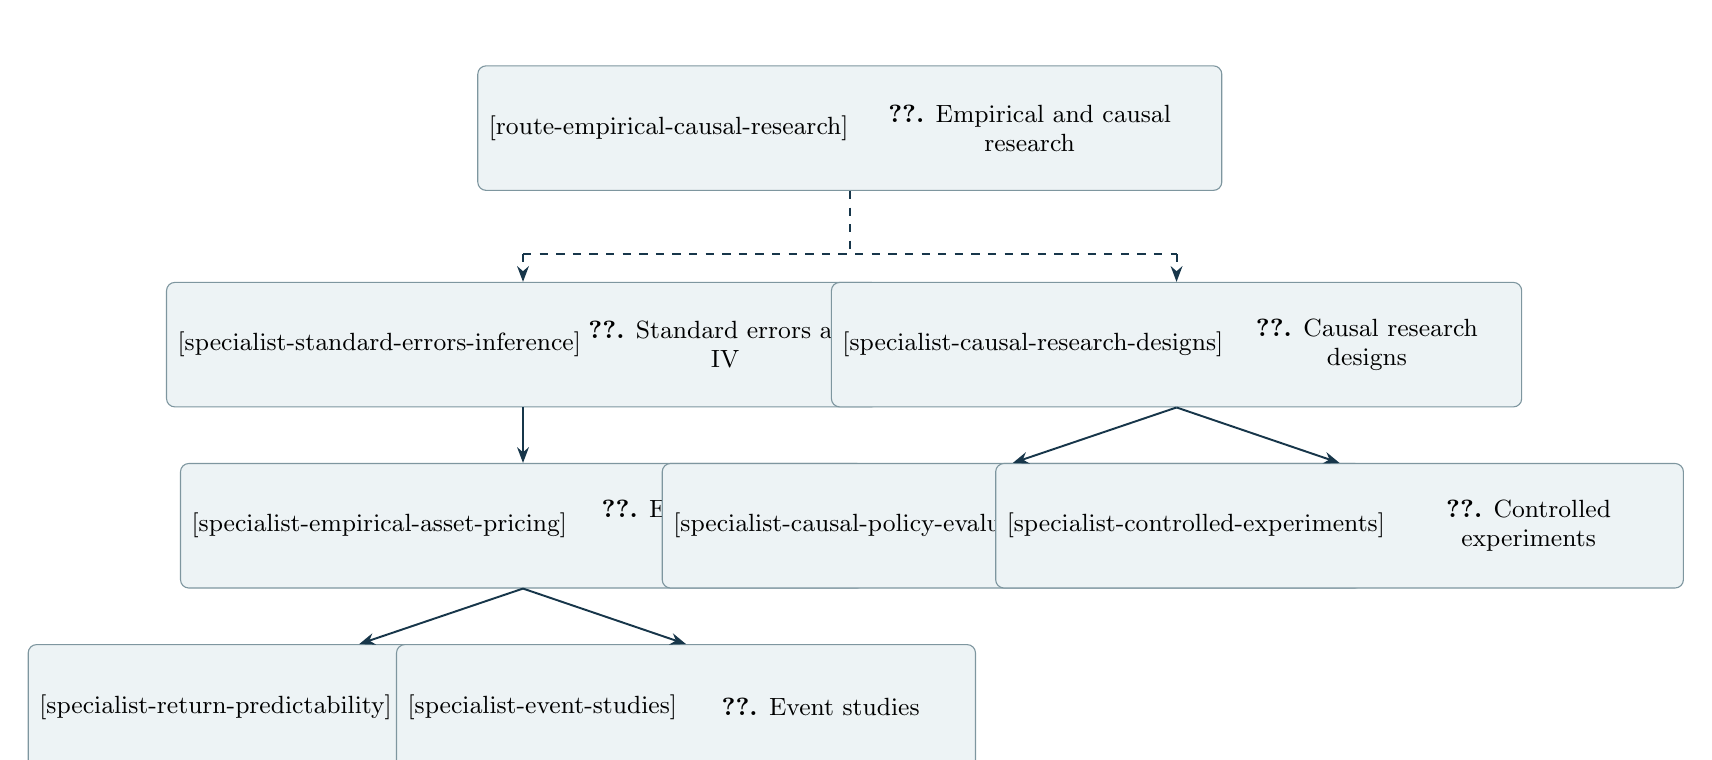
\begin{tikzpicture}[x=1cm,y=1cm]
\node[pathnode] (empirical-causal-research) at (6.23,0) {\MeasurePathNode{4.6cm}{\textbf{\ref*{route-empirical-causal-research}.} Empirical and causal research}\hyperref[route-empirical-causal-research]{\parbox[c][\pathnodeheight][c]{4.6cm}{\centering \textbf{\ref*{route-empirical-causal-research}.} Empirical and causal research}}};
\node[pathnode] (standard-errors-inference) at (2.08,-2.75) {\MeasurePathNode{3.65cm}{\textbf{\ref*{specialist-standard-errors-inference}.} Standard errors and IV}\hyperref[specialist-standard-errors-inference]{\parbox[c][\pathnodeheight][c]{3.65cm}{\centering \textbf{\ref*{specialist-standard-errors-inference}.} Standard errors and IV}}};
\node[pathnode] (causal-research-designs) at (10.38,-2.75) {\MeasurePathNode{3.65cm}{\textbf{\ref*{specialist-causal-research-designs}.} Causal research designs}\hyperref[specialist-causal-research-designs]{\parbox[c][\pathnodeheight][c]{3.65cm}{\centering \textbf{\ref*{specialist-causal-research-designs}.} Causal research designs}}};
\node[pathnode] (empirical-asset-pricing) at (2.08,-5.05) {\MeasurePathNode{3.65cm}{\textbf{\ref*{specialist-empirical-asset-pricing}.} Empirical asset pricing}\hyperref[specialist-empirical-asset-pricing]{\parbox[c][\pathnodeheight][c]{3.65cm}{\centering \textbf{\ref*{specialist-empirical-asset-pricing}.} Empirical asset pricing}}};
\node[pathnode] (causal-policy-evaluation) at (8.30,-5.05) {\MeasurePathNode{3.65cm}{\textbf{\ref*{specialist-causal-policy-evaluation}.} Causal ML and financial policy evaluation}\hyperref[specialist-causal-policy-evaluation]{\parbox[c][\pathnodeheight][c]{3.65cm}{\centering \textbf{\ref*{specialist-causal-policy-evaluation}.} Causal ML and financial policy evaluation}}};
\node[pathnode] (controlled-experiments) at (12.45,-5.05) {\MeasurePathNode{3.65cm}{\textbf{\ref*{specialist-controlled-experiments}.} Controlled experiments}\hyperref[specialist-controlled-experiments]{\parbox[c][\pathnodeheight][c]{3.65cm}{\centering \textbf{\ref*{specialist-controlled-experiments}.} Controlled experiments}}};
\node[pathnode] (return-predictability) at (0.00,-7.35) {\MeasurePathNode{3.65cm}{\textbf{\ref*{specialist-return-predictability}.} Predictability and forecast tests}\hyperref[specialist-return-predictability]{\parbox[c][\pathnodeheight][c]{3.65cm}{\centering \textbf{\ref*{specialist-return-predictability}.} Predictability and forecast tests}}};
\node[pathnode] (event-studies) at (4.15,-7.35) {\MeasurePathNode{3.65cm}{\textbf{\ref*{specialist-event-studies}.} Event studies}\hyperref[specialist-event-studies]{\parbox[c][\pathnodeheight][c]{3.65cm}{\centering \textbf{\ref*{specialist-event-studies}.} Event studies}}};
\draw[entryline] (empirical-causal-research.south) -- (6.23,-1.60);
\draw[entryline] (2.08,-1.60) -- (10.38,-1.60);
\draw[entryarrow] (2.08,-1.60) -- (standard-errors-inference.north);
\draw[entryarrow] (10.38,-1.60) -- (causal-research-designs.north);
\draw[patharrow] (standard-errors-inference.south) -- (empirical-asset-pricing.north);
\draw[patharrow] (causal-research-designs.south) -- (causal-policy-evaluation.north);
\draw[patharrow] (causal-research-designs.south) -- (controlled-experiments.north);
\draw[patharrow] (empirical-asset-pricing.south) -- (return-predictability.north);
\draw[patharrow] (empirical-asset-pricing.south) -- (event-studies.north);
\end{tikzpicture}\end{center}
\textbf{Bring these foundations with you.}\begin{itemize}
\item \hyperref[specialist-time-series-volatility]{Time-series econometrics and volatility forecasting} --- needed by \hyperref[specialist-return-predictability]{Predictability and forecast tests}.
\end{itemize}\hyperref[learning-map]{Return to the whole-guide DAG.}
\Needspace{12\baselineskip}
\subsection{Standard errors, clustering and weak instruments}\label{specialist-standard-errors-inference}
\textbf{Specialist pathway.} In \hyperref[route-empirical-causal-research]{Empirical asset pricing and causal inference}.

\textbf{Outcome.} Choose and justify standard errors for a financial panel or time-series regression, and report instrumental-variable results with first-stage strength and weak-instrument-robust inference.

\textbf{Prerequisites.} Empirical asset pricing and causal inference overview; OLS, IV and panel regression. Probability, statistical inference and econometric theory (1.1) helps.

\textbf{Review first.} \hyperref[route-empirical-causal-research]{Empirical asset pricing and causal inference}.

\textbf{Required readings, in order}
\begin{enumerate}\raggedright
\Needspace{5\baselineskip}\item \href{institutional_quantitative_finance_reading_list.pdf\#rf-white-1980}{Halbert White, ``A Heteroskedasticity-Consistent Covariance Matrix Estimator and a Direct Test for Heteroskedasticity''}\CataloguePage{46}\NoteKey{rf-white-1980}\par \textbf{Foundations.} Start from heteroskedasticity-consistent covariance estimation.
\Needspace{5\baselineskip}\item \href{institutional_quantitative_finance_reading_list.pdf\#catalogue-0735}{Whitney K. Newey and Kenneth D. West, ``A Simple, Positive Semi-Definite, Heteroskedasticity and Autocorrelation Consistent Covariance Matrix\textquotesingle\textquotesingle (1986 technical working paper; 1987 journal article)}\CataloguePage{86}\NoteKey{catalogue-0735}\par \textbf{Foundations.} Add autocorrelation with the Newey--West HAC estimator.
\Needspace{5\baselineskip}\item \href{institutional_quantitative_finance_reading_list.pdf\#rf-andrews-1991}{Donald W. K. Andrews, ``Heteroskedasticity and Autocorrelation Consistent Covariance Matrix Estimation''}\CataloguePage{46}\NoteKey{rf-andrews-1991}\par \textbf{Methods.} Choose the HAC kernel and bandwidth by a stated criterion rather than habit.
\Needspace{5\baselineskip}\item \href{institutional_quantitative_finance_reading_list.pdf\#rf-petersen-2009}{Mitchell A. Petersen, ``Estimating Standard Errors in Finance Panel Data Sets: Comparing Approaches''}\CataloguePage{46}\NoteKey{rf-petersen-2009}\par \textbf{Methods.} Learn when clustering, Fama--MacBeth and other panel corrections agree and when they diverge.
\Needspace{5\baselineskip}\item \href{institutional_quantitative_finance_reading_list.pdf\#rf-thompson-2011}{Samuel B. Thompson, ``Simple formulas for standard errors that cluster by both firm and time''}\CataloguePage{46}\NoteKey{rf-thompson-2011}\par \textbf{Methods.} Cluster by firm and time together with a simple formula.
\Needspace{5\baselineskip}\item \href{institutional_quantitative_finance_reading_list.pdf\#rf-cameron-gelbach-miller-2011}{A. Colin Cameron, Jonah B. Gelbach and Douglas L. Miller, ``Robust Inference With Multiway Clustering''}\CataloguePage{47}\NoteKey{rf-cameron-gelbach-miller-2011}\par \textbf{Methods.} Extend clustering to non-nested multiway dependence and nonlinear estimators.
\Needspace{5\baselineskip}\item \href{institutional_quantitative_finance_reading_list.pdf\#rf-cameron-miller-2015}{A. Colin Cameron and Douglas L. Miller, ``A Practitioner’s Guide to Cluster-Robust Inference''}\CataloguePage{47}\NoteKey{rf-cameron-miller-2015}\par \textbf{Implementation.} Handle fixed effects, few clusters and multiway clustering in practice.
\Needspace{5\baselineskip}\item \href{institutional_quantitative_finance_reading_list.pdf\#rf-gow-ormazabal-taylor-2010}{Ian D. Gow, Gaizka Ormazabal and Daniel J. Taylor, ``Correcting for Cross-Sectional and Time-Series Dependence in Accounting Research''}\CataloguePage{47}\NoteKey{rf-gow-ormazabal-taylor-2010}\par \textbf{Evidence.} See published inferences change once both cross-sectional and time-series dependence are corrected.
\Needspace{5\baselineskip}\item \href{institutional_quantitative_finance_reading_list.pdf\#rf-abadie-athey-imbens-wooldridge-2023}{Alberto Abadie, Susan Athey, Guido W. Imbens and Jeffrey M. Wooldridge, ``When Should You Adjust Standard Errors for Clustering?''}\CataloguePage{47}\NoteKey{rf-abadie-athey-imbens-wooldridge-2023}\par \textbf{Theory.} Decide whether to cluster from the sampling and assignment design, not by convention.
\Needspace{5\baselineskip}\item \href{institutional_quantitative_finance_reading_list.pdf\#rf-bertrand-duflo-mullainathan-2004}{Marianne Bertrand, Esther Duflo and Sendhil Mullainathan, ``How Much Should We Trust Differences-In-Differences Estimates?''}\CataloguePage{47}\NoteKey{rf-bertrand-duflo-mullainathan-2004}\par \textbf{Evidence.} Measure how serially correlated outcomes inflate difference-in-differences significance.
\Needspace{5\baselineskip}\item \href{institutional_quantitative_finance_reading_list.pdf\#rf-stambaugh-1999}{Robert F. Stambaugh, ``Predictive regressions''}\CataloguePage{47}\NoteKey{rf-stambaugh-1999}\par \textbf{Theory.} Correct predictive-regression bias when the regressor is persistent.
\Needspace{5\baselineskip}\item \href{institutional_quantitative_finance_reading_list.pdf\#rf-jiang-2017}{Wei Jiang, ``Have Instrumental Variables Brought Us Closer to the Truth''}\CataloguePage{48}\NoteKey{rf-jiang-2017}\par \textbf{Evidence.} Compare IV and OLS magnitudes across published finance papers before trusting a large IV estimate.
\Needspace{5\baselineskip}\item \href{institutional_quantitative_finance_reading_list.pdf\#rf-andrews-stock-sun-2019}{Isaiah Andrews, James H. Stock and Liyang Sun, ``Weak Instruments in Instrumental Variables Regression: Theory and Practice''}\CataloguePage{48}\NoteKey{rf-andrews-stock-sun-2019}\par \textbf{Methods.} Detect weak instruments and use robust confidence sets with clustered or serially correlated data.
\Needspace{5\baselineskip}\item \href{institutional_quantitative_finance_reading_list.pdf\#rf-lee-mccrary-moreira-porter-2022}{David S. Lee, Justin McCrary, Marcelo J. Moreira and Jack Porter, ``Valid <i>t</i>-ratio Inference for IV''}\CataloguePage{48}\NoteKey{rf-lee-mccrary-moreira-porter-2022}\par \textbf{Validation.} Adjust single-instrument t-ratio inference for first-stage strength.
\Needspace{5\baselineskip}\item \href{institutional_quantitative_finance_reading_list.pdf\#rf-young-2022}{Alwyn Young, ``Consistency without Inference: Instrumental Variables in Practical Application''}\CataloguePage{48}\NoteKey{rf-young-2022}\par \textbf{Counter-evidence.} See how often IV inference in published papers fails size, power and pre-test checks.
\Needspace{5\baselineskip}\item \href{institutional_quantitative_finance_reading_list.pdf\#exp-nonstandard-errors}{Albert J. Menkveld et al. (FINance Crowd Analysis Project), Nonstandard Errors}\CataloguePage{83}\NoteKey{exp-nonstandard-errors}\par \textbf{Validation.} Add the variation across analysts to sampling error when reporting uncertainty.
\end{enumerate}
\Needspace{5\baselineskip}\textbf{Checkpoint.} Regress monthly stock returns on a lagged characteristic in a firm-month panel and report OLS, White, firm-clustered, month-clustered, two-way clustered, Driscoll--Kraay and Newey--West-adjusted Fama--MacBeth standard errors; explain the differences from the residual correlation structure. For one IV specification from a published paper, report the effective first-stage F, the tF-adjusted interval and an Anderson--Rubin interval.

\textbf{Optional branches.} \href{institutional_quantitative_finance_reading_list.pdf\#rf-driscoll-kraay-1998}{Use covariance estimators robust to cross-sectional and temporal dependence in long panels.}\BranchPage{47} \href{institutional_quantitative_finance_reading_list.pdf\#rf-hodrick-1992}{Compare inference procedures for long-horizon return regressions.}\BranchPage{48} \href{institutional_quantitative_finance_reading_list.pdf\#rf-stock-yogo-2005}{Read the source of the weak-instrument critical values.}\BranchPage{48} \href{institutional_quantitative_finance_reading_list.pdf\#wide-shanken-1992}{Correct two-pass standard errors for estimated betas.}\BranchPage{28} \href{institutional_quantitative_finance_reading_list.pdf\#wide-hayashi-econometrics}{Revise GMM and HAC inference.}\BranchPage{36}
\par{\small \hyperref[learning-map]{Learning pathway DAG} \textbar{} \hyperref[route-empirical-causal-research]{Section overview} \textbar{} \hyperref[map-empirical-causal-research]{Section DAG}\NoteKey{standard-errors-inference}}
\Needspace{12\baselineskip}
\subsection{Causal research designs: DiD, synthetic control and RD}\label{specialist-causal-research-designs}
\textbf{Specialist pathway.} In \hyperref[route-empirical-causal-research]{Empirical asset pricing and causal inference}.

\textbf{Outcome.} Choose an identification design for a policy, regulation or corporate event and test its assumptions before estimating effects.

\textbf{Prerequisites.} Regression and potential-outcome notation.

\textbf{Review first.} \hyperref[route-empirical-causal-research]{Empirical asset pricing and causal inference}.

\textbf{Required readings, in order}
\begin{enumerate}\raggedright
\Needspace{5\baselineskip}\item \href{institutional_quantitative_finance_reading_list.pdf\#wide-cunningham-mixtape}{Scott Cunningham, \emph{Causal Inference: The Mixtape}}\CataloguePage{73}\NoteKey{wide-cunningham-mixtape}\par \textbf{Foundations.} Learn DAGs and the main design-based estimators with code.
\Needspace{5\baselineskip}\item \href{institutional_quantitative_finance_reading_list.pdf\#wide-huntington-klein-effect}{Nick Huntington-Klein, \emph{The Effect: An Introduction to Research Design and Causality}}\CataloguePage{73}\NoteKey{wide-huntington-klein-effect}\par \textbf{Foundations.} Work through research design before estimation.
\Needspace{5\baselineskip}\item \href{institutional_quantitative_finance_reading_list.pdf\#catalogue-0813}{Angrist and Pischke, \emph{Mostly Harmless Econometrics}}\CataloguePage{73}\NoteKey{catalogue-0813}\par \textbf{Methods.} Review IV, regression and DiD logic.
\Needspace{5\baselineskip}\item \href{institutional_quantitative_finance_reading_list.pdf\#wide-goodman-bacon}{Andrew Goodman-Bacon, ``Difference-in-differences with variation in treatment timing''}\CataloguePage{74}\NoteKey{wide-goodman-bacon}\par \textbf{Methods.} See why two-way fixed effects fail with staggered timing.
\Needspace{5\baselineskip}\item \href{institutional_quantitative_finance_reading_list.pdf\#wide-callaway-santanna}{Brantly Callaway and Pedro H. C. Sant'Anna, ``Difference-in-Differences with multiple time periods''}\CataloguePage{73}\NoteKey{wide-callaway-santanna}\par \textbf{Methods.} Estimate group-time effects robust to staggered adoption.
\Needspace{5\baselineskip}\item \href{institutional_quantitative_finance_reading_list.pdf\#wide-roth-did-review}{Jonathan Roth, Pedro H. C. Sant'Anna, Alyssa Bilinski and John Poe, ``What's trending in difference-in-differences? A synthesis of the recent econometrics literature''}\CataloguePage{74}\NoteKey{wide-roth-did-review}\par \textbf{Validation.} Assess parallel trends, sensitivity and inference.
\Needspace{5\baselineskip}\item \href{institutional_quantitative_finance_reading_list.pdf\#wide-abadie-synthetic}{Alberto Abadie, ``Using Synthetic Controls: Feasibility, Data Requirements, and Methodological Aspects''}\CataloguePage{73}\NoteKey{wide-abadie-synthetic}\par \textbf{Methods.} Use synthetic controls with adequate pre-period fit.
\Needspace{5\baselineskip}\item \href{institutional_quantitative_finance_reading_list.pdf\#wide-arkhangelsky-sdid}{Dmitry Arkhangelsky, Susan Athey, David A. Hirshberg, Guido W. Imbens and Stefan Wager, ``Synthetic Difference-in-Differences''}\CataloguePage{74}\NoteKey{wide-arkhangelsky-sdid}\par \textbf{Methods.} Combine synthetic-control weights with DiD.
\Needspace{5\baselineskip}\item \href{institutional_quantitative_finance_reading_list.pdf\#wide-cattaneo-rd}{Matias D. Cattaneo, Nicolás Idrobo and Rocío Titiunik, \emph{A Practical Introduction to Regression Discontinuity Designs: Foundations}}\CataloguePage{74}\NoteKey{wide-cattaneo-rd}\par \textbf{Methods.} Estimate regression-discontinuity effects with robust bandwidths.
\Needspace{5\baselineskip}\item \href{institutional_quantitative_finance_reading_list.pdf\#wide-roberts-whited}{Michael R. Roberts and Toni M. Whited, ``Endogeneity in Empirical Corporate Finance''}\CataloguePage{74}\NoteKey{wide-roberts-whited}\par \textbf{Evidence.} Map these designs to finance-specific endogeneity problems.
\Needspace{5\baselineskip}\item \href{institutional_quantitative_finance_reading_list.pdf\#w5-baker-larcker-wang-did}{Andrew C. Baker, David F. Larcker and Charles C. Y. Wang, ``How much should we trust staggered difference-in-differences estimates?''}\CataloguePage{75}\NoteKey{w5-baker-larcker-wang-did}\par \textbf{Validation.} Check staggered DiD designs for negative weighting in finance settings.
\end{enumerate}
\Needspace{5\baselineskip}\textbf{Checkpoint.} Pick a staggered financial regulation (for example a reporting rule or index inclusion), estimate its effect with TWFE, Callaway--Sant'Anna and synthetic DiD, and report pre-trends, sensitivity bounds and which estimates you would publish.

\textbf{Optional branches.} \href{institutional_quantitative_finance_reading_list.pdf\#wide-pearl-causality}{Formalise identification with structural causal models.}\BranchPage{74} \href{institutional_quantitative_finance_reading_list.pdf\#w3-nyborg-woschitz-did}{Run DiD on term-structure outcomes.}\BranchPage{74} \href{institutional_quantitative_finance_reading_list.pdf\#w3-cohn-past-prologue}{Consider pre-event return patterns in event studies.}\BranchPage{74} \href{institutional_quantitative_finance_reading_list.pdf\#w4-lopezdeprado-zoonekynd-factor-mirage}{Avoid collider bias in factor-model specification.}\BranchPage{53} \href{institutional_quantitative_finance_reading_list.pdf\#w4-olivetti-adia-causal-challenge}{Compare supervised and constraint-based causal discovery.}\BranchPage{76} \href{institutional_quantitative_finance_reading_list.pdf\#w5-sun-abraham}{Estimate event-study dynamics robust to heterogeneity.}\BranchPage{75} \href{institutional_quantitative_finance_reading_list.pdf\#w5-dechaisemartin-dhaultfoeuille}{Diagnose negative weights in TWFE.}\BranchPage{75} \href{institutional_quantitative_finance_reading_list.pdf\#rf-borusyak-jaravel-spiess-2024}{Estimate staggered-adoption designs with an efficient imputation estimator.}\BranchPage{46}
\par{\small \hyperref[learning-map]{Learning pathway DAG} \textbar{} \hyperref[route-empirical-causal-research]{Section overview} \textbar{} \hyperref[map-empirical-causal-research]{Section DAG}\NoteKey{causal-research-designs}}
\Needspace{12\baselineskip}
\subsection{Empirical asset pricing: factor models and tests}\label{specialist-empirical-asset-pricing}
\textbf{Specialist pathway.} In \hyperref[route-empirical-causal-research]{Empirical asset pricing and causal inference}.

\textbf{Outcome.} Estimate and test a factor model with correct standard errors, then decide whether a new factor adds pricing information.

\textbf{Prerequisites.} Standard errors, clustering and weak instruments (2.1); regression and GMM basics.

\textbf{Review first.} \hyperref[route-empirical-causal-research]{Empirical asset pricing and causal inference}; \hyperref[specialist-standard-errors-inference]{Standard errors, clustering and weak instruments}.

\textbf{Required readings, in order}
\begin{enumerate}\raggedright
\Needspace{5\baselineskip}\item \href{institutional_quantitative_finance_reading_list.pdf\#wide-fama-macbeth}{Eugene F. Fama and James D. MacBeth, ``Risk, Return, and Equilibrium: Empirical Tests''}\CataloguePage{28}\NoteKey{wide-fama-macbeth}\par \textbf{Methods.} Run cross-sectional regressions averaged through time.
\Needspace{5\baselineskip}\item \href{institutional_quantitative_finance_reading_list.pdf\#wide-shanken-1992}{Jay Shanken, ``On the Estimation of Beta-Pricing Models''}\CataloguePage{28}\NoteKey{wide-shanken-1992}\par \textbf{Methods.} Correct two-pass standard errors for estimated betas.
\Needspace{5\baselineskip}\item \href{institutional_quantitative_finance_reading_list.pdf\#wide-grs-1989}{Michael R. Gibbons, Stephen A. Ross and Jay Shanken, ``A Test of the Efficiency of a Given Portfolio''}\CataloguePage{28}\NoteKey{wide-grs-1989}\par \textbf{Validation.} Test whether factor portfolios span the test assets.
\Needspace{5\baselineskip}\item \href{institutional_quantitative_finance_reading_list.pdf\#wide-hansen-gmm}{Lars Peter Hansen, ``Large Sample Properties of Generalized Method of Moments Estimators''}\CataloguePage{28}\NoteKey{wide-hansen-gmm}\par \textbf{Theory.} Estimate SDF models from moment conditions.
\Needspace{5\baselineskip}\item \href{institutional_quantitative_finance_reading_list.pdf\#wide-bali-engle-murray}{Turan G. Bali, Robert F. Engle and Scott Murray, \emph{Empirical Asset Pricing: The Cross Section of Stock Returns}}\CataloguePage{29}\NoteKey{wide-bali-engle-murray}\par \textbf{Implementation.} Follow a practical guide to sorts, regressions and data screens.
\Needspace{5\baselineskip}\item \href{institutional_quantitative_finance_reading_list.pdf\#alpha-ff1993}{Eugene Fama and Kenneth French, ``Common Risk Factors in the Returns on Stocks and Bonds''}\CataloguePage{192}\NoteKey{alpha-ff1993}\par \textbf{Evidence.} Read the three-factor model as the benchmark.
\Needspace{5\baselineskip}\item \href{institutional_quantitative_finance_reading_list.pdf\#wide-ff-five-factor}{Eugene F. Fama and Kenneth R. French, ``A five-factor asset pricing model''}\CataloguePage{28}\NoteKey{wide-ff-five-factor}\par \textbf{Evidence.} Compare profitability and investment additions.
\Needspace{5\baselineskip}\item \href{institutional_quantitative_finance_reading_list.pdf\#wide-hxz-q-factor}{Kewei Hou, Chen Xue and Lu Zhang, ``Digesting Anomalies: An Investment Approach''}\CataloguePage{29}\NoteKey{wide-hxz-q-factor}\par \textbf{Evidence.} Compare the investment-based q-factor model.
\Needspace{5\baselineskip}\item \href{institutional_quantitative_finance_reading_list.pdf\#wide-kps-ipca}{Bryan T. Kelly, Seth Pruitt and Yinan Su, ``Characteristics are covariances: A unified model of risk and return''}\CataloguePage{29}\NoteKey{wide-kps-ipca}\par \textbf{Methods.} Let characteristics drive loadings with IPCA.
\Needspace{5\baselineskip}\item \href{institutional_quantitative_finance_reading_list.pdf\#wide-kozak-nagel-santosh}{Serhiy Kozak, Stefan Nagel and Shrihari Santosh, ``Shrinking the cross-section''}\CataloguePage{29}\NoteKey{wide-kozak-nagel-santosh}\par \textbf{Methods.} Shrink SDF coefficients across many characteristics.
\Needspace{5\baselineskip}\item \href{institutional_quantitative_finance_reading_list.pdf\#wide-feng-giglio-xiu-zoo}{Guanhao Feng, Stefano Giglio and Dacheng Xiu, ``Taming the Factor Zoo: A Test of New Factors''}\CataloguePage{29}\NoteKey{wide-feng-giglio-xiu-zoo}\par \textbf{Validation.} Test new factors against a high-dimensional set.
\Needspace{5\baselineskip}\item \href{institutional_quantitative_finance_reading_list.pdf\#wide-bhj-factor-zoo}{Svetlana Bryzgalova, Jiantao Huang and Christian Julliard, ``Bayesian Solutions for the Factor Zoo: We Just Ran Two Quadrillion Models''}\CataloguePage{29}\NoteKey{wide-bhj-factor-zoo}\par \textbf{Validation.} Average across models when no single model dominates.
\Needspace{5\baselineskip}\item \href{institutional_quantitative_finance_reading_list.pdf\#exp-jkp-replication}{Theis Ingerslev Jensen, Bryan Kelly, and Lasse Heje Pedersen, Is There a Replication Crisis in Finance?; Project data and documentation}\CataloguePage{87}\NoteKey{exp-jkp-replication}\par \textbf{Evidence.} Check replication and global evidence for factor premia.
\end{enumerate}
\Needspace{5\baselineskip}\textbf{Checkpoint.} Using public factor and portfolio data, estimate CAPM, FF3, FF5 and q-factor models on the same test assets; report Fama--MacBeth premia with Shanken corrections, GRS statistics and the incremental contribution of one new factor under double-selection lasso.

\textbf{Optional branches.} \href{institutional_quantitative_finance_reading_list.pdf\#wide-giglio-xiu-omitted}{Estimate risk premia robust to omitted factors.}\BranchPage{29} \href{institutional_quantitative_finance_reading_list.pdf\#wide-cochrane-discount-rates}{Read the discount-rate perspective on the factor zoo.}\BranchPage{29} \href{institutional_quantitative_finance_reading_list.pdf\#section.2.1}{Browse the asset-pricing foundations section.}\BranchPage{27} \href{institutional_quantitative_finance_reading_list.pdf\#w2-pennacchi}{Use an accessible asset-pricing theory text.}\BranchPage{27} \href{institutional_quantitative_finance_reading_list.pdf\#w3-bryzgalova-forest-trees}{Build test assets with AP-Trees.}\BranchPage{55} \href{institutional_quantitative_finance_reading_list.pdf\#w3-dickerson-copricing-zoo}{Price bonds and stocks jointly across a factor zoo.}\BranchPage{30} \href{institutional_quantitative_finance_reading_list.pdf\#w3-ait-sahalia-cont-fmb}{Run continuous-time Fama--MacBeth with jumps.}\BranchPage{30} \href{institutional_quantitative_finance_reading_list.pdf\#exp-replicating-anomalies}{Rebuild a large anomaly library under common conventions.}\BranchPage{87} \href{institutional_quantitative_finance_reading_list.pdf\#exp-open-source-ap}{Reuse open-source code for published characteristics.}\BranchPage{87}
\par{\small \hyperref[learning-map]{Learning pathway DAG} \textbar{} \hyperref[route-empirical-causal-research]{Section overview} \textbar{} \hyperref[map-empirical-causal-research]{Section DAG}\NoteKey{empirical-asset-pricing}}
\Needspace{12\baselineskip}
\subsection{Causal ML and financial policy evaluation}\label{specialist-causal-policy-evaluation}
\textbf{Specialist pathway.} In \hyperref[route-empirical-causal-research]{Empirical asset pricing and causal inference}.

\textbf{Outcome.} Distinguish a predictive association from the effect of an execution, quote or allocation policy, and evaluate how confounding and market spillovers change the conclusion.

\textbf{Prerequisites.} Regression, conditional expectation and the common toolkit; an explicit treatment, outcome and decision timestamp.

\textbf{Review first.} \hyperref[route-empirical-causal-research]{Empirical asset pricing and causal inference}; \hyperref[specialist-causal-research-designs]{Causal research designs: DiD, synthetic control and RD}.

\textbf{Required readings, in order}
\begin{enumerate}\raggedright
\Needspace{5\baselineskip}\item \href{institutional_quantitative_finance_reading_list.pdf\#s3-kohavi}{Ron Kohavi, Diane Tang and Ya Xu, \emph{Trustworthy Online Controlled Experiments: A Practical Guide to A/B Testing}}\CataloguePage{78}\NoteKey{s3-kohavi}\par \textbf{Design.} Define a primary outcome, assignment unit, guardrails and stopping rule before estimating an effect.
\Needspace{5\baselineskip}\item \href{institutional_quantitative_finance_reading_list.pdf\#latest-causal-ml-book}{Victor Chernozhukov, Christian Hansen, Nathan Kallus, Martin Spindler and Vasilis Syrgkanis, \emph{Applied Causal Inference Powered by ML and AI}; Fixed original arXiv version}\CataloguePage{75}\NoteKey{latest-causal-ml-book}\par\emph{Selection:} Randomized-experiment and double/debiased-ML material; match notebooks to the selected author-site version.\par \textbf{Identification and estimation.} Work through randomized assignment, adjustment and DML examples; distinguish assumptions about treatment assignment from nuisance-model prediction.
\Needspace{5\baselineskip}\item \href{institutional_quantitative_finance_reading_list.pdf\#catalogue-0808}{Victor Chernozhukov et al., ``Double/Debiased Machine Learning for Treatment and Structural Parameters''}\CataloguePage{75}\NoteKey{catalogue-0808}\par \textbf{Inference.} Study orthogonal scores and cross-fitting, including the sampling assumptions that need adaptation for dependent financial observations.
\Needspace{5\baselineskip}\item \href{institutional_quantitative_finance_reading_list.pdf\#latest-causal-omitted-variable-bias}{Victor Chernozhukov, Carlos Cinelli, Whitney K. Newey, Amit Sharma and Vasilis Syrgkanis, Long Story Short: Omitted Variable Bias in Causal Machine Learning; Journal DOI}\CataloguePage{76}\NoteKey{latest-causal-omitted-variable-bias}\par \textbf{Sensitivity.} Quantify how unobserved confounding could change the sign or economic size of an estimated effect.
\Needspace{5\baselineskip}\item \href{institutional_quantitative_finance_reading_list.pdf\#s3-johari}{Ramesh Johari, Hannah Li, Inessa Liskovich and Gabriel Y. Weintraub, ``Experimental Design in Two-Sided Platforms: An Analysis of Bias''; preprint}\CataloguePage{76}\NoteKey{s3-johari}\par \textbf{Market interactions.} Check whether one order or participant changes outcomes for other units, violating a no-interference assumption.
\Needspace{5\baselineskip}\item \href{institutional_quantitative_finance_reading_list.pdf\#exp-policy-learning-observational}{Susan Athey and Stefan Wager, Policy Learning With Observational Data}\CataloguePage{75}\NoteKey{exp-policy-learning-observational}\par \textbf{Decision.} Separate effect estimation from learning a constrained policy on observational data.
\Needspace{5\baselineskip}\item \href{institutional_quantitative_finance_reading_list.pdf\#w5-wager-athey-cf}{Stefan Wager and Susan Athey, ``Estimation and Inference of Heterogeneous Treatment Effects using Random Forests''}\CataloguePage{76}\NoteKey{w5-wager-athey-cf}\par \textbf{Methods.} Estimate heterogeneous effects with causal forests and valid intervals.
\Needspace{5\baselineskip}\item \href{institutional_quantitative_finance_reading_list.pdf\#w5-kunzel-metalearners}{Sören R. Künzel, Jasjeet S. Sekhon, Peter J. Bickel and Bin Yu, ``Metalearners for estimating heterogeneous treatment effects using machine learning''}\CataloguePage{77}\NoteKey{w5-kunzel-metalearners}\par \textbf{Methods.} Compare S-, T- and X-learners for conditional effects.
\Needspace{5\baselineskip}\item \href{institutional_quantitative_finance_reading_list.pdf\#w5-nie-wager-rlearner}{X. Nie and S. Wager, ``Quasi-oracle estimation of heterogeneous treatment effects''}\CataloguePage{77}\NoteKey{w5-nie-wager-rlearner}\par \textbf{Methods.} Make heterogeneous-effect estimation robust to nuisance errors.
\end{enumerate}
\Needspace{5\baselineskip}\textbf{Checkpoint.} Design a simulated quote-policy or execution experiment. Specify assignment, delayed outcomes and spillovers; estimate a known treatment effect with cross-fitting and a dependence-appropriate split. Introduce an omitted confounder and report sensitivity ranges. Evaluate the learned policy on an untouched sample and explain what would still prevent a causal claim on observational market data.

\textbf{Optional branches.} \href{institutional_quantitative_finance_reading_list.pdf\#section.4.1}{Use the full identification and experimental-design chapter when the policy or assignment mechanism requires a different design.}\BranchPage{73} \href{institutional_quantitative_finance_reading_list.pdf\#w5-athey-imbens-ml-econ}{Survey ML methods for economists.}\BranchPage{77} \href{institutional_quantitative_finance_reading_list.pdf\#w5-belloni-pds}{Select controls by post-double-selection lasso.}\BranchPage{77}
\par{\small \hyperref[learning-map]{Learning pathway DAG} \textbar{} \hyperref[route-empirical-causal-research]{Section overview} \textbar{} \hyperref[map-empirical-causal-research]{Section DAG}\NoteKey{causal-policy-evaluation}}
\Needspace{12\baselineskip}
\subsection{Controlled experiments: A/B tests, switchbacks and sequential monitoring}\label{specialist-controlled-experiments}
\textbf{Specialist pathway.} In \hyperref[route-empirical-causal-research]{Empirical asset pricing and causal inference}.

\textbf{Outcome.} Design, monitor and analyse a randomised test of a trading, quoting or platform change with a pre-registered metric, adequate power, valid stopping and checks for interference and assignment failures.

\textbf{Prerequisites.} Causal research designs (2.2). Kohavi, Tang and Xu in causal ML and financial policy evaluation (2.4) is a helpful companion.

\textbf{Review first.} \hyperref[route-empirical-causal-research]{Empirical asset pricing and causal inference}; \hyperref[specialist-causal-research-designs]{Causal research designs: DiD, synthetic control and RD}.

\textbf{Required readings, in order}
\begin{enumerate}\raggedright
\Needspace{5\baselineskip}\item \href{institutional_quantitative_finance_reading_list.pdf\#s3-gerber}{Alan S. Gerber and Donald P. Green, \emph{Field Experiments: Design, Analysis, and Interpretation}}\CataloguePage{77}\NoteKey{s3-gerber}\par \textbf{Foundations.} Learn randomisation, blocking, clustering, compliance and analysis for field experiments.
\Needspace{5\baselineskip}\item \href{institutional_quantitative_finance_reading_list.pdf\#rf-larsen-2024}{Nicholas Larsen, Jonathan Stallrich, Srijan Sengupta, Alex Deng, Ron Kohavi and Nathaniel T. Stevens, ``Statistical Challenges in Online Controlled Experiments: A Review of A/B Testing Methodology''}\CataloguePage{79}\NoteKey{rf-larsen-2024}\par \textbf{Foundations.} Survey the statistical problems raised by large-scale online experiments.
\Needspace{5\baselineskip}\item \href{institutional_quantitative_finance_reading_list.pdf\#al-cuped}{Alex Deng, Ya Xu, Ron Kohavi and Toby Walker, ``Improving the Sensitivity of Online Controlled Experiments by Utilizing Pre-Experiment Data''}\CataloguePage{78}\NoteKey{al-cuped}\par \textbf{Methods.} Reduce variance with pre-experiment covariates.
\Needspace{5\baselineskip}\item \href{institutional_quantitative_finance_reading_list.pdf\#al-srm}{Aleksander Fabijan et al., ``Diagnosing Sample Ratio Mismatch in Online Controlled Experiments: A Taxonomy and Rules of Thumb for Practitioners''}\CataloguePage{79}\NoteKey{al-srm}\par \textbf{Validation.} Diagnose sample-ratio mismatch before reading any effect.
\Needspace{5\baselineskip}\item \href{institutional_quantitative_finance_reading_list.pdf\#rf-johari-koomen-pekelis-walsh-2022}{Ramesh Johari, Pete Koomen, Leonid Pekelis and David Walsh, ``Always Valid Inference: Continuous Monitoring of A/B Tests''}\CataloguePage{79}\NoteKey{rf-johari-koomen-pekelis-walsh-2022}\par \textbf{Methods.} Monitor a test continuously with always-valid p-values.
\Needspace{5\baselineskip}\item \href{institutional_quantitative_finance_reading_list.pdf\#al-howard}{Steven R. Howard, Aaditya Ramdas, Jon McAuliffe and Jasjeet Sekhon, ``Time-uniform, Nonparametric, Nonasymptotic Confidence Sequences''; author preprint}\CataloguePage{79}\NoteKey{al-howard}\par \textbf{Methods.} Build confidence sequences that hold at every stopping time.
\Needspace{5\baselineskip}\item \href{institutional_quantitative_finance_reading_list.pdf\#al-switchback}{Iavor Bojinov, David Simchi-Levi and Jinglong Zhao, ``Design and Analysis of Switchback Experiments''}\CataloguePage{78}\NoteKey{al-switchback}\par \textbf{Methods.} Randomise over time blocks when units interact, with explicit carryover assumptions.
\Needspace{5\baselineskip}\item \href{institutional_quantitative_finance_reading_list.pdf\#al-aronow}{Peter M. Aronow and Cyrus Samii, ``Estimating Average Causal Effects Under General Interference, with Application to a Social Network Experiment''}\CataloguePage{78}\NoteKey{al-aronow}\par \textbf{Theory.} Estimate effects under a stated exposure model for interference.
\Needspace{5\baselineskip}\item \href{institutional_quantitative_finance_reading_list.pdf\#s3-holtz}{David Holtz, Felipe Lobel, Ruben Lobel, Inessa Liskovich and Sinan Aral, ``Reducing Interference Bias in Online Marketplace Experiments Using Cluster Randomization: Evidence from a Pricing Meta-experiment on Airbnb''}\CataloguePage{78}\NoteKey{s3-holtz}\par \textbf{Evidence.} Compare individual and cluster randomisation when units are substitutes.
\Needspace{5\baselineskip}\item \href{institutional_quantitative_finance_reading_list.pdf\#s3-wu}{Yuhang Wu, Zeyu Zheng, Guangyu Zhang, Zuohua Zhang and Chu Wang, ``Non-Stationary A/B Tests''}\CataloguePage{76}\NoteKey{s3-wu}\par \textbf{Methods.} Handle non-stationary treatment effects with time-aware randomisation and post-stratification.
\Needspace{5\baselineskip}\item \href{institutional_quantitative_finance_reading_list.pdf\#s3-webster}{Kevin Webster and Nicholas Westray, ``Getting More for Less: Better A/B Testing via Causal Regularization''}\CataloguePage{76}\NoteKey{s3-webster}\par \textbf{Implementation.} Combine observational trading data with costly interventional experiments for alpha and impact.
\Needspace{5\baselineskip}\item \href{institutional_quantitative_finance_reading_list.pdf\#al-surrogate}{Susan Athey, Raj Chetty, Guido W. Imbens and Hyunseung Kang, ``The Surrogate Index: Combining Short-Term Proxies to Estimate Long-Term Treatment Effects More Rapidly and Precisely''; NBER version}\CataloguePage{79}\NoteKey{al-surrogate}\par \textbf{Methods.} Infer long-run effects from short-run proxies only under stated conditions.
\end{enumerate}
\Needspace{5\baselineskip}\textbf{Checkpoint.} Design an experiment comparing two execution algorithms: choose the randomisation unit (parent order, symbol-day or time block), pre-register implementation shortfall as the primary metric with guardrails, compute power from historical fills with and without CUPED, specify an always-valid stopping rule and a sample-ratio check, then simulate the test on historical data with a planted effect and report the false-positive rate under peeking.

\textbf{Optional branches.} \href{institutional_quantitative_finance_reading_list.pdf\#s3-montgomery}{Use factorial and blocked designs when several parameters change at once.}\BranchPage{77} \href{institutional_quantitative_finance_reading_list.pdf\#s3-spotify}{Handle sequential tests with repeated observations.}\BranchPage{78} \href{institutional_quantitative_finance_reading_list.pdf\#s3-uber}{Read a practitioner account of an internal experimentation platform.}\BranchPage{78} \href{institutional_quantitative_finance_reading_list.pdf\#al-hadad}{Make inference after adaptive (bandit) assignment.}\BranchPage{79} \href{institutional_quantitative_finance_reading_list.pdf\#al-dudik}{Evaluate a new policy off-line from logged decisions.}\BranchPage{79} \href{institutional_quantitative_finance_reading_list.pdf\#s3-handbook}{Compare laboratory and field approaches in experimental finance.}\BranchPage{78}
\par{\small \hyperref[learning-map]{Learning pathway DAG} \textbar{} \hyperref[route-empirical-causal-research]{Section overview} \textbar{} \hyperref[map-empirical-causal-research]{Section DAG}\NoteKey{controlled-experiments}}
\Needspace{12\baselineskip}
\subsection{Return predictability and forecast evaluation}\label{specialist-return-predictability}
\textbf{Specialist pathway.} In \hyperref[route-empirical-causal-research]{Empirical asset pricing and causal inference}.

\textbf{Outcome.} Judge an aggregate return predictor with present-value logic, out-of-sample tests for nested models and proper scoring.

\textbf{Prerequisites.} Time-series econometrics and empirical asset pricing.

\textbf{Review first.} \hyperref[specialist-time-series-volatility]{Time-series econometrics and volatility forecasting}; \hyperref[specialist-empirical-asset-pricing]{Empirical asset pricing: factor models and tests}.

\textbf{Required readings, in order}
\begin{enumerate}\raggedright
\Needspace{5\baselineskip}\item \href{institutional_quantitative_finance_reading_list.pdf\#wide-campbell-shiller-1988}{John Y. Campbell and Robert J. Shiller, ``The Dividend-Price Ratio and Expectations of Future Dividends and Discount Factors''}\CataloguePage{31}\NoteKey{wide-campbell-shiller-1988}\par \textbf{Theory.} Use the log-linear present-value identity to interpret valuation ratios.
\Needspace{5\baselineskip}\item \href{institutional_quantitative_finance_reading_list.pdf\#wide-cochrane-dog}{John H. Cochrane, ``The Dog That Did Not Bark: A Defense of Return Predictability''}\CataloguePage{31}\NoteKey{wide-cochrane-dog}\par \textbf{Theory.} Link return and dividend-growth predictability.
\Needspace{5\baselineskip}\item \href{institutional_quantitative_finance_reading_list.pdf\#s7-welch}{\emph{Ivo Welch and Amit Goyal, ``A Comprehensive Look at the Empirical Performance of Equity Premium Prediction'' (2008)}}\CataloguePage{31}\NoteKey{s7-welch}\par \textbf{Evidence.} See why most predictors failed out of sample in 2008.
\Needspace{5\baselineskip}\item \href{institutional_quantitative_finance_reading_list.pdf\#wide-goyal-welch-zafirov}{Amit Goyal, Ivo Welch and Athanasse Zafirov, ``A Comprehensive 2022 Look at the Empirical Performance of Equity Premium Prediction''}\CataloguePage{31}\NoteKey{wide-goyal-welch-zafirov}\par \textbf{Evidence.} Use the updated predictor set and sample.
\Needspace{5\baselineskip}\item \href{institutional_quantitative_finance_reading_list.pdf\#wide-campbell-thompson}{John Y. Campbell and Samuel B. Thompson, ``Predicting Excess Stock Returns Out of Sample: Can Anything Beat the Historical Average?''}\CataloguePage{31}\NoteKey{wide-campbell-thompson}\par \textbf{Methods.} Impose economic restrictions on forecasts.
\Needspace{5\baselineskip}\item \href{institutional_quantitative_finance_reading_list.pdf\#wide-rapach-strauss-zhou}{David E. Rapach, Jack K. Strauss and Guofu Zhou, ``Out-of-Sample Equity Premium Prediction: Combination Forecasts and Links to the Real Economy''}\CataloguePage{31}\NoteKey{wide-rapach-strauss-zhou}\par \textbf{Methods.} Combine forecasts instead of selecting one.
\Needspace{5\baselineskip}\item \href{institutional_quantitative_finance_reading_list.pdf\#wide-clark-west}{Todd E. Clark and Kenneth D. West, ``Approximately normal tests for equal predictive accuracy in nested models''}\CataloguePage{86}\NoteKey{wide-clark-west}\par \textbf{Validation.} Test nested models fairly against the historical mean.
\Needspace{5\baselineskip}\item \href{institutional_quantitative_finance_reading_list.pdf\#wide-giacomini-white}{Raffaella Giacomini and Halbert White, ``Tests of Conditional Predictive Ability''}\CataloguePage{86}\NoteKey{wide-giacomini-white}\par \textbf{Validation.} Evaluate forecasting methods conditionally with rolling windows.
\Needspace{5\baselineskip}\item \href{institutional_quantitative_finance_reading_list.pdf\#wide-gneiting-raftery}{Tilmann Gneiting and Adrian E. Raftery, ``Strictly Proper Scoring Rules, Prediction, and Estimation''}\CataloguePage{39}\NoteKey{wide-gneiting-raftery}\par \textbf{Validation.} Score density and interval forecasts with proper rules.
\Needspace{5\baselineskip}\item \href{institutional_quantitative_finance_reading_list.pdf\#wide-martin-svix}{Ian Martin, ``What is the Expected Return on the Market?''}\CataloguePage{31}\NoteKey{wide-martin-svix}\par \textbf{Evidence.} Compare a forward-looking option-based premium bound.
\Needspace{5\baselineskip}\item \href{institutional_quantitative_finance_reading_list.pdf\#w3-cakici-pockets-replication}{Nusret Cakici, Christian Fieberg, Tobias Neumaier, Thorsten Poddig and Adam Zaremba, ``Pockets of Predictability: A Replication''}\CataloguePage{32}\NoteKey{w3-cakici-pockets-replication}\par \textbf{Validation.} Check that kernel predictability uses only one-sided, real-time information.
\end{enumerate}
\Needspace{5\baselineskip}\textbf{Checkpoint.} Replicate an out-of-sample equity-premium exercise with five predictors, sign restrictions and a combination forecast; report Clark--West tests, the certainty-equivalent gain for a mean-variance investor and how results change with the start of the evaluation sample.

\textbf{Optional branches.} \href{institutional_quantitative_finance_reading_list.pdf\#wide-timmermann-combinations}{Study forecast-combination weights in depth.}\BranchPage{39} \href{institutional_quantitative_finance_reading_list.pdf\#section.5.2}{Browse the forecast-comparison and inference readings.}\BranchPage{82} \href{institutional_quantitative_finance_reading_list.pdf\#w3-li-dominate-average}{Use a conservative constant slope to beat the historical mean.}\BranchPage{32} \href{institutional_quantitative_finance_reading_list.pdf\#w3-vanbinsbergen-lucky-survivor}{Adjust the US premium for survivorship.}\BranchPage{32} \href{institutional_quantitative_finance_reading_list.pdf\#w3-dahlquist-ibert-expectations}{Compare institutional capital-market assumptions.}\BranchPage{32} \href{institutional_quantitative_finance_reading_list.pdf\#w3-delao-return-dominance}{Decompose valuation dispersion into returns and growth.}\BranchPage{32} \href{institutional_quantitative_finance_reading_list.pdf\#w4-tasitsiomi-effective-complexity}{Measure effective rather than nominal model complexity.}\BranchPage{56} \href{institutional_quantitative_finance_reading_list.pdf\#rf-stambaugh-1999}{Correct predictive-regression bias with persistent regressors.}\BranchPage{47} \href{institutional_quantitative_finance_reading_list.pdf\#rf-hodrick-1992}{Compare long-horizon inference procedures.}\BranchPage{48}
\par{\small \hyperref[learning-map]{Learning pathway DAG} \textbar{} \hyperref[route-empirical-causal-research]{Section overview} \textbar{} \hyperref[map-empirical-causal-research]{Section DAG}\NoteKey{return-predictability}}
\Needspace{12\baselineskip}
\subsection{Event studies and long-run abnormal returns}\label{specialist-event-studies}
\textbf{Specialist pathway.} In \hyperref[route-empirical-causal-research]{Empirical asset pricing and causal inference}.

\textbf{Outcome.} Measure the price effect of a corporate, policy or information event at short and long horizons with a stated normal-return model and test statistics that are correctly sized under event clustering and variance changes.

\textbf{Prerequisites.} Empirical asset pricing: factor models and tests (2.3), for normal-return models and characteristic benchmarks; it brings Standard errors, clustering and weak instruments (2.1) with it.

\textbf{Review first.} \hyperref[route-empirical-causal-research]{Empirical asset pricing and causal inference}; \hyperref[specialist-empirical-asset-pricing]{Empirical asset pricing: factor models and tests}.

\textbf{Required readings, in order}
\begin{enumerate}\raggedright
\Needspace{5\baselineskip}\item \href{institutional_quantitative_finance_reading_list.pdf\#rf-fama-fisher-jensen-roll-1969}{Eugene F. Fama, Lawrence Fisher, Michael C. Jensen and Richard Roll, ``The Adjustment of Stock Prices to New Information''}\CataloguePage{45}\NoteKey{rf-fama-fisher-jensen-roll-1969}\par \textbf{Foundations.} Read the first event study, of stock splits, and the question it was built to answer.
\Needspace{5\baselineskip}\item \href{institutional_quantitative_finance_reading_list.pdf\#rf-mackinlay-1997}{A. Craig MacKinlay, ``Event Studies in Economics and Finance''}\CataloguePage{46}\NoteKey{rf-mackinlay-1997}\par \textbf{Foundations.} Learn the standard event-study procedure step by step.
\Needspace{5\baselineskip}\item \href{institutional_quantitative_finance_reading_list.pdf\#eq-kothari-warner-2007}{S. P. Kothari and Jerold B. Warner, ``Econometrics of Event Studies''}\CataloguePage{207}\NoteKey{eq-kothari-warner-2007}\par \textbf{Foundations.} Survey short- and long-horizon event-study design and the limits of each.
\Needspace{5\baselineskip}\item \href{institutional_quantitative_finance_reading_list.pdf\#rf-brown-warner-1980}{Stephen J. Brown and Jerold B. Warner, ``Measuring security price performance''}\CataloguePage{45}\NoteKey{rf-brown-warner-1980}\par \textbf{Methods.} Compare normal-return models by simulating abnormal performance in actual returns.
\Needspace{5\baselineskip}\item \href{institutional_quantitative_finance_reading_list.pdf\#rf-brown-warner-1985}{Stephen J. Brown and Jerold B. Warner, ``Using daily stock returns''}\CataloguePage{44}\NoteKey{rf-brown-warner-1985}\par \textbf{Methods.} Learn the market-model event study on daily data and when simple tests are well specified.
\Needspace{5\baselineskip}\item \href{institutional_quantitative_finance_reading_list.pdf\#rf-boehmer-musumeci-poulsen-1991}{Ekkehart Boehmer, Jim Musumeci and Annette B. Poulsen, ``Event-study methodology under conditions of event-induced variance''}\CataloguePage{44}\NoteKey{rf-boehmer-musumeci-poulsen-1991}\par \textbf{Methods.} Standardise abnormal returns so that event-induced variance does not inflate rejection rates.
\Needspace{5\baselineskip}\item \href{institutional_quantitative_finance_reading_list.pdf\#rf-kolari-pynnonen-2010}{James W. Kolari and Seppo Pynnönen, ``Event Study Testing with Cross-sectional Correlation of Abnormal Returns''}\CataloguePage{44}\NoteKey{rf-kolari-pynnonen-2010}\par \textbf{Validation.} Correct the test for cross-correlation when event dates cluster.
\Needspace{5\baselineskip}\item \href{institutional_quantitative_finance_reading_list.pdf\#rf-kolari-pynnonen-2011}{James W. Kolari and Seppo Pynnonen, ``Nonparametric rank tests for event studies''}\CataloguePage{45}\NoteKey{rf-kolari-pynnonen-2011}\par \textbf{Methods.} Use a rank test that works for cumulative abnormal returns.
\Needspace{5\baselineskip}\item \href{institutional_quantitative_finance_reading_list.pdf\#rf-barber-lyon-1997}{Brad M. Barber and John D. Lyon, ``Detecting long-run abnormal stock returns: The empirical power and specification of test statistics''}\CataloguePage{44}\NoteKey{rf-barber-lyon-1997}\par \textbf{Methods.} Use size and book-to-market matched control firms for long-run abnormal returns.
\Needspace{5\baselineskip}\item \href{institutional_quantitative_finance_reading_list.pdf\#eq-lyon-barber-tsai-1999}{John D. Lyon, Brad M. Barber and Chih-Ling Tsai, ``Improved Methods for Tests of Long-Run Abnormal Stock Returns''}\CataloguePage{207}\NoteKey{eq-lyon-barber-tsai-1999}\par \textbf{Methods.} Use reference portfolios with skewness-adjusted or bootstrapped tests, or calendar-time portfolios.
\Needspace{5\baselineskip}\item \href{institutional_quantitative_finance_reading_list.pdf\#rf-daniel-grinblatt-titman-wermers-1997}{Kent Daniel, Mark Grinblatt, Sheridan Titman and Russ Wermers, ``Measuring Mutual Fund Performance with Characteristic‐Based Benchmarks''}\CataloguePage{45}\NoteKey{rf-daniel-grinblatt-titman-wermers-1997}\par \textbf{Methods.} Build characteristic-matched (DGTW) benchmark returns.
\Needspace{5\baselineskip}\item \href{institutional_quantitative_finance_reading_list.pdf\#eq-fama-1998}{Eugene F. Fama, ``Market Efficiency, Long-Term Returns, and Behavioral Finance''}\CataloguePage{207}\NoteKey{eq-fama-1998}\par \textbf{Evidence.} Read the case that long-run anomalies are fragile to method.
\Needspace{5\baselineskip}\item \href{institutional_quantitative_finance_reading_list.pdf\#rf-mitchell-stafford-2000}{Mark L. Mitchell and Erik Stafford, ``Managerial Decisions and Long‐Term Stock Price Performance''}\CataloguePage{45}\NoteKey{rf-mitchell-stafford-2000}\par \textbf{Validation.} See cross-sectional dependence inflate long-run test statistics and calendar-time tests correct it.
\Needspace{5\baselineskip}\item \href{institutional_quantitative_finance_reading_list.pdf\#rf-loughran-ritter-2000}{Tim Loughran and Jay R. Ritter, ``Uniformly least powerful tests of market efficiency''}\CataloguePage{45}\NoteKey{rf-loughran-ritter-2000}\par \textbf{Counter-evidence.} Read the reply that long-run tests lack power, not that the anomalies are fragile.
\Needspace{5\baselineskip}\item \href{institutional_quantitative_finance_reading_list.pdf\#rf-goldsmith-pinkham-lyu-2025}{Paul Goldsmith-Pinkham and Tianshu Lyu, ``Causal Inference in Financial Event Studies''}\CataloguePage{46}\NoteKey{rf-goldsmith-pinkham-lyu-2025}\par \textbf{Validation.} Check whether factor-model misspecification biases long-horizon or volatile-period estimates.
\end{enumerate}
\Needspace{5\baselineskip}\textbf{Checkpoint.} Run an event study of S\&P 500 index additions (or another announcement type with public dates). Report market-model and characteristic-matched abnormal returns over a 3-day window and over 12 and 36 months; compare the ordinary, BMP, Kolari--Pynnönen and GRANK tests for the short window and buy-and-hold versus calendar-time portfolio inference for the long window, and explain any disagreement.

\textbf{Optional branches.} \href{institutional_quantitative_finance_reading_list.pdf\#s15-campbell}{Read the event-study chapter of the standard financial-econometrics text.}\BranchPage{35} \href{institutional_quantitative_finance_reading_list.pdf\#rf-corrado-2011}{Survey short-horizon event-study methodology, including rank tests.}\BranchPage{45} \href{institutional_quantitative_finance_reading_list.pdf\#rf-borusyak-jaravel-spiess-2024}{Use imputation estimators for staggered panel event-study designs.}\BranchPage{46} \href{institutional_quantitative_finance_reading_list.pdf\#wide-bessembinder-bond-abnormal}{Adapt event-study methods to daily corporate-bond data.}\BranchPage{520} \href{institutional_quantitative_finance_reading_list.pdf\#w3-cohn-past-prologue}{Check pre-event return patterns before attributing a reaction to the event.}\BranchPage{74} \href{institutional_quantitative_finance_reading_list.pdf\#w5-sun-abraham}{Estimate dynamic event-study effects robust to heterogeneous timing.}\BranchPage{75}
\par{\small \hyperref[learning-map]{Learning pathway DAG} \textbar{} \hyperref[route-empirical-causal-research]{Section overview} \textbar{} \hyperref[map-empirical-causal-research]{Section DAG}\NoteKey{event-studies}}
\clearpage
\section{Research engineering and validation}\label{route-research-engineering-validation}
\label{route-11}
\textbf{Learning sequence.} Make data availability, research records, code and trading events auditable and reproducible before assessing model evidence.

\textbf{Section goals.} Across its pathways, this section teaches you to:
\begin{itemize}[leftmargin=1.4em,itemsep=0pt,topsep=1pt]
\item report backtests with multiplicity-adjusted significance and Sharpe-ratio uncertainty (\hyperref[specialist-backtest-inference]{\ref*{specialist-backtest-inference}})
\item build research panels whose every field was available at decision time (\hyperref[specialist-point-in-time-data]{\ref*{specialist-point-in-time-data}})
\item design model inventories, validation and pre-trade controls (\hyperref[specialist-model-governance-controls]{\ref*{specialist-model-governance-controls}})
\item package research so that it rebuilds from raw inputs and can be monitored in production (\hyperref[specialist-reproducible-research-code]{\ref*{specialist-reproducible-research-code}})
\end{itemize}
\textbf{Overview outcome.} Reconstruct a research decision and its eventual trade from versioned identities, data events, experiments and control records.

\textbf{Prerequisites.} Common toolkit; database joins, event logs, version control and basic trading lifecycle terms.

\textbf{Review first.} \hyperref[route-common-toolkit]{Common toolkit}.

\textbf{Required readings, in order}
\begin{enumerate}\raggedright
\Needspace{5\baselineskip}\item \href{institutional_quantitative_finance_reading_list.pdf\#exp-gleif}{Global Legal Entity Identifier Foundation (GLEIF), Golden Copy and Delta Files}\CataloguePage{517}\NoteKey{exp-gleif}\par Start with durable entity identities and delta updates rather than matching display names.
\Needspace{5\baselineskip}\item \href{institutional_quantitative_finance_reading_list.pdf\#exp-crsp-ciz}{CRSP, CRSP US Stock and Indexes Databases: Summary of CIZ Differences to Legacy Files}\CataloguePage{517}\NoteKey{exp-crsp-ciz}\par Test how a dataset format change alters security history and return construction.
\Needspace{5\baselineskip}\item \href{institutional_quantitative_finance_reading_list.pdf\#exp-cdm}{FINOS, with ISDA, ICMA and ISLA, Common Domain Model: Overview and Event Model; documentation and event model}\CataloguePage{518}\NoteKey{exp-cdm}\par Represent economic terms and lifecycle events as explicit trade-state transitions.
\Needspace{5\baselineskip}\item \href{institutional_quantitative_finance_reading_list.pdf\#s6-fix}{FIX Trading Community, \emph{Online Specification}}\CataloguePage{530}\NoteKey{s6-fix}\par Connect submitted orders, acknowledgments, fills and cancels to protocol-level evidence.
\Needspace{5\baselineskip}\item \href{institutional_quantitative_finance_reading_list.pdf\#s8-bitemporal}{Martin Fowler, \emph{Bitemporal History} (2021)}\CataloguePage{531}\NoteKey{s8-bitemporal}\par Retain both effective and known-at times through corrections and restatements.
\Needspace{5\baselineskip}\item \href{institutional_quantitative_finance_reading_list.pdf\#s6-ddia}{Martin Kleppmann and Chris Riccomini, \emph{Designing Data-Intensive Applications}, 2nd ed.}\CataloguePage{531}\NoteKey{s6-ddia}\par Reason about logs, consistency and replay failure in data-intensive systems.
\Needspace{5\baselineskip}\item \href{institutional_quantitative_finance_reading_list.pdf\#s8-mlflow}{MLflow; 3.16.0 release notes}\CataloguePage{532}\NoteKey{s8-mlflow}\par Track code, inputs, parameters and model artifacts for each experiment.
\Needspace{5\baselineskip}\item \href{institutional_quantitative_finance_reading_list.pdf\#exp-bcbs239}{Basel Committee on Banking Supervision, Principles for Effective Risk Data Aggregation and Risk Reporting (BCBS 239)}\CataloguePage{535}\NoteKey{exp-bcbs239}\par Check whether risk data remain complete, timely and reconcilable across institutional systems.
\end{enumerate}
\Needspace{5\baselineskip}\textbf{Checkpoint.} Take one signal decision through raw source, normalized identity, historical revision, model run, order and final position. Produce a replay package that reproduces the decision and P\&L after a corrected input arrives, including the failed run and reconciliation differences.

\textbf{Optional branches.} \href{institutional_quantitative_finance_reading_list.pdf\#section.22.2}{Deepen model-risk, clearing and settlement controls.}\BranchPage{539} \href{institutional_quantitative_finance_reading_list.pdf\#section.8.5}{Add replayable market scenarios for execution evaluation.}\BranchPage{166} \href{institutional_quantitative_finance_reading_list.pdf\#wide-sandve-ten-rules}{Adopt simple reproducibility rules.}\BranchPage{81} \href{institutional_quantitative_finance_reading_list.pdf\#wide-wilson-good-enough}{Apply good-enough computing practices.}\BranchPage{534}
\par\textbf{Continue in this section.} \hyperref[specialist-backtest-inference]{Backtest inference, multiple testing and Sharpe-ratio statistics}; \hyperref[specialist-point-in-time-data]{Point-in-time data, vendor files and bias control}; \hyperref[specialist-model-governance-controls]{Model governance, AI risk and trading controls}; \hyperref[specialist-reproducible-research-code]{Reproducible research code, data validation and ML systems}.
\par{\small \hyperref[learning-map]{Learning pathway DAG} \textbar{} \hyperref[map-research-engineering-validation]{Section DAG}\NoteKey{research-engineering-validation}}
\clearpage
\subsection*{Research engineering and validation: pathway DAG}\phantomsection\label{map-research-engineering-validation}
\addcontentsline{toc}{subsection}{Research engineering and validation: pathway DAG}
Start with the section overview's readings, for orientation. Solid arrows show prerequisites within this section. Dashed connectors identify entry points with no further prerequisite in this section; the linked foundations below still apply. Follow the arrows for dependencies and the subsection numbers for reading order. Every node is clickable.
\begin{center}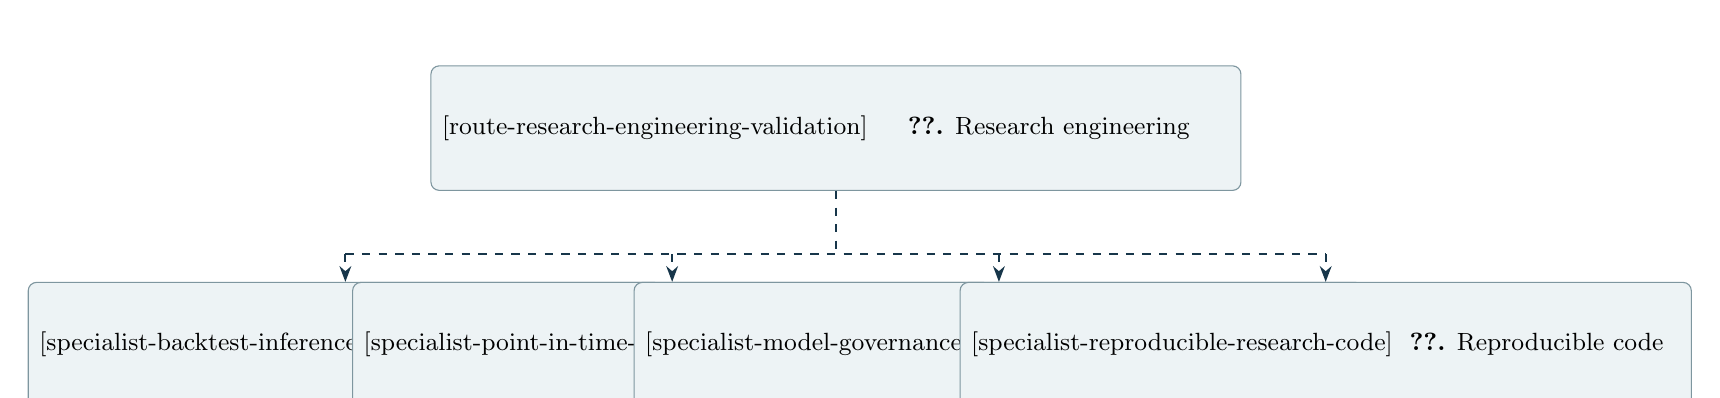
\begin{tikzpicture}[x=1cm,y=1cm]
\node[pathnode] (research-engineering-validation) at (6.23,0) {\MeasurePathNode{4.6cm}{\textbf{\ref*{route-research-engineering-validation}.} Research engineering}\hyperref[route-research-engineering-validation]{\parbox[c][\pathnodeheight][c]{4.6cm}{\centering \textbf{\ref*{route-research-engineering-validation}.} Research engineering}}};
\node[pathnode] (backtest-inference) at (0.00,-2.75) {\MeasurePathNode{3.65cm}{\textbf{\ref*{specialist-backtest-inference}.} Backtest inference}\hyperref[specialist-backtest-inference]{\parbox[c][\pathnodeheight][c]{3.65cm}{\centering \textbf{\ref*{specialist-backtest-inference}.} Backtest inference}}};
\node[pathnode] (point-in-time-data) at (4.15,-2.75) {\MeasurePathNode{3.65cm}{\textbf{\ref*{specialist-point-in-time-data}.} Point-in-time data}\hyperref[specialist-point-in-time-data]{\parbox[c][\pathnodeheight][c]{3.65cm}{\centering \textbf{\ref*{specialist-point-in-time-data}.} Point-in-time data}}};
\node[pathnode] (model-governance-controls) at (8.30,-2.75) {\MeasurePathNode{3.65cm}{\textbf{\ref*{specialist-model-governance-controls}.} Governance and controls}\hyperref[specialist-model-governance-controls]{\parbox[c][\pathnodeheight][c]{3.65cm}{\centering \textbf{\ref*{specialist-model-governance-controls}.} Governance and controls}}};
\node[pathnode] (reproducible-research-code) at (12.45,-2.75) {\MeasurePathNode{3.65cm}{\textbf{\ref*{specialist-reproducible-research-code}.} Reproducible code}\hyperref[specialist-reproducible-research-code]{\parbox[c][\pathnodeheight][c]{3.65cm}{\centering \textbf{\ref*{specialist-reproducible-research-code}.} Reproducible code}}};
\draw[entryline] (research-engineering-validation.south) -- (6.23,-1.60);
\draw[entryline] (0.00,-1.60) -- (12.45,-1.60);
\draw[entryarrow] (0.00,-1.60) -- (backtest-inference.north);
\draw[entryarrow] (4.15,-1.60) -- (point-in-time-data.north);
\draw[entryarrow] (8.30,-1.60) -- (model-governance-controls.north);
\draw[entryarrow] (12.45,-1.60) -- (reproducible-research-code.north);
\end{tikzpicture}\end{center}
\textbf{Bring these foundations with you.}\begin{itemize}
\item \hyperref[route-common-toolkit]{Common toolkit} --- needed by \hyperref[specialist-backtest-inference]{Backtest inference}.
\end{itemize}\hyperref[learning-map]{Return to the whole-guide DAG.}
\Needspace{12\baselineskip}
\subsection{Backtest inference, multiple testing and Sharpe-ratio statistics}\label{specialist-backtest-inference}
\textbf{Specialist pathway.} In \hyperref[route-research-engineering-validation]{Research engineering and validation}.

\textbf{Outcome.} Report a strategy result with the number of trials, multiplicity-adjusted significance and Sharpe-ratio uncertainty under dependence.

\textbf{Prerequisites.} Statistics, bootstrap and the common toolkit.

\textbf{Review first.} \hyperref[route-research-engineering-validation]{Research engineering and validation}; \hyperref[route-common-toolkit]{Common toolkit}.

\textbf{Required readings, in order}
\begin{enumerate}\raggedright
\Needspace{5\baselineskip}\item \href{institutional_quantitative_finance_reading_list.pdf\#wide-harvey-scientific-outlook}{Campbell R. Harvey, ``Presidential Address: The Scientific Outlook in Financial Economics''}\CataloguePage{81}\NoteKey{wide-harvey-scientific-outlook}\par \textbf{Foundations.} Understand p-hacking incentives in finance research.
\Needspace{5\baselineskip}\item \href{institutional_quantitative_finance_reading_list.pdf\#wide-arnott-harvey-markowitz}{Rob Arnott, Campbell R. Harvey and Harry Markowitz, ``A Backtesting Protocol in the Era of Machine Learning''}\CataloguePage{81}\NoteKey{wide-arnott-harvey-markowitz}\par \textbf{Methods.} Adopt a backtesting protocol before running experiments.
\Needspace{5\baselineskip}\item \href{institutional_quantitative_finance_reading_list.pdf\#catalogue-0731}{White (2000), \textquotedblleft A Reality Check for Data Snooping\textquotedblright}\CataloguePage{82}\NoteKey{catalogue-0731}\par \textbf{Methods.} Apply White's Reality Check to a family of rules.
\Needspace{5\baselineskip}\item \href{institutional_quantitative_finance_reading_list.pdf\#wide-romano-wolf-stepdown}{Joseph P. Romano and Michael Wolf, ``Stepwise Multiple Testing as Formalized Data Snooping''}\CataloguePage{83}\NoteKey{wide-romano-wolf-stepdown}\par \textbf{Methods.} Identify which strategies survive with stepdown control.
\Needspace{5\baselineskip}\item \href{institutional_quantitative_finance_reading_list.pdf\#wide-benjamini-hochberg}{Yoav Benjamini and Yosef Hochberg, ``Controlling the False Discovery Rate: A Practical and Powerful Approach to Multiple Testing''}\CataloguePage{83}\NoteKey{wide-benjamini-hochberg}\par \textbf{Methods.} Control the false-discovery rate when screening many signals.
\Needspace{5\baselineskip}\item \href{institutional_quantitative_finance_reading_list.pdf\#alpha-harvey}{Campbell Harvey, Yan Liu and Heqing Zhu, ``...and the Cross-Section of Expected Returns''}\CataloguePage{82}\NoteKey{alpha-harvey}\par \textbf{Evidence.} Raise significance thresholds for the factor zoo.
\Needspace{5\baselineskip}\item \href{institutional_quantitative_finance_reading_list.pdf\#wide-chordia-goyal-saretto}{Tarun Chordia, Amit Goyal and Alessio Saretto, ``Anomalies and False Rejections''}\CataloguePage{83}\NoteKey{wide-chordia-goyal-saretto}\par \textbf{Evidence.} Calibrate thresholds with millions of mined signals.
\Needspace{5\baselineskip}\item \href{institutional_quantitative_finance_reading_list.pdf\#wide-lo-sharpe}{Andrew W. Lo, ``The Statistics of Sharpe Ratios''}\CataloguePage{84}\NoteKey{wide-lo-sharpe}\par \textbf{Validation.} Compute Sharpe-ratio standard errors with serial correlation.
\Needspace{5\baselineskip}\item \href{institutional_quantitative_finance_reading_list.pdf\#wide-ledoit-wolf-sharpe}{Oliver Ledoit and Michael Wolf, ``Robust performance hypothesis testing with the Sharpe ratio''}\CataloguePage{84}\NoteKey{wide-ledoit-wolf-sharpe}\par \textbf{Validation.} Test differences between Sharpe ratios robustly.
\Needspace{5\baselineskip}\item \href{institutional_quantitative_finance_reading_list.pdf\#wide-politis-romano-stationary}{Dimitris N. Politis and Joseph P. Romano, ``The Stationary Bootstrap''}\CataloguePage{85}\NoteKey{wide-politis-romano-stationary}\par \textbf{Methods.} Resample dependent returns with the stationary bootstrap.
\Needspace{5\baselineskip}\item \href{institutional_quantitative_finance_reading_list.pdf\#alpha-dsr}{David H. Bailey and Marcos López de Prado, ``The Deflated Sharpe Ratio: Correcting for Selection Bias, Backtest Overfitting and Non-Normality'' (author copy)}\CataloguePage{82}\NoteKey{alpha-dsr}\par \textbf{Validation.} Deflate the Sharpe ratio for trials and non-normality.
\Needspace{5\baselineskip}\item \href{institutional_quantitative_finance_reading_list.pdf\#wide-kapoor-narayanan-leakage}{Sayash Kapoor and Arvind Narayanan, ``Leakage and the reproducibility crisis in machine-learning-based science''}\CataloguePage{81}\NoteKey{wide-kapoor-narayanan-leakage}\par \textbf{Validation.} Audit the pipeline for the main types of leakage.
\Needspace{5\baselineskip}\item \href{institutional_quantitative_finance_reading_list.pdf\#w3-duarte-lookahead-options}{Jefferson Duarte, Christopher S. Jones, Mehdi Khorram, Haitao Mo and Junbo L. Wang, ``Too Good to Be True: Look-Ahead Bias in Empirical Options Research''}\CataloguePage{84}\NoteKey{w3-duarte-lookahead-options}\par \textbf{Validation.} Detect look-ahead from filtering noisy quotes with future information.
\Needspace{5\baselineskip}\item \href{institutional_quantitative_finance_reading_list.pdf\#w3-zhang-man-vs-ml-revisited}{Yingguang Zhang, Yandi Zhu and Juhani T. Linnainmaa, ``Man versus Machine Learning Revisited''}\CataloguePage{55}\NoteKey{w3-zhang-man-vs-ml-revisited}\par \textbf{Validation.} See a high-profile ML alpha disappear once look-ahead is removed.
\Needspace{5\baselineskip}\item \href{institutional_quantitative_finance_reading_list.pdf\#w4-lopezdeprado-sr-inference}{Marcos López de Prado, Alexander Lipton and Vincent Zoonekynd, ``Sharpe Ratio Inference: A New Standard for Decision Making and Reporting''}\CataloguePage{85}\NoteKey{w4-lopezdeprado-sr-inference}\par \textbf{Validation.} Report Sharpe ratios with significance, power and non-Normal corrections.
\Needspace{5\baselineskip}\item \href{institutional_quantitative_finance_reading_list.pdf\#w4-lopezdeprado-porcu-dsr}{Marcos López de Prado and Emilio Porcu, ``The Deflated Sharpe Ratio: A Unified Framework for Search-Adjusted Performance Inference''}\CataloguePage{84}\NoteKey{w4-lopezdeprado-porcu-dsr}\par \textbf{Validation.} Deflate the winning Sharpe ratio for the size of the search.
\end{enumerate}
\Needspace{5\baselineskip}\textbf{Checkpoint.} Generate 200 variants of a simple signal, record every trial, and report the best Sharpe ratio with Lo standard errors, a deflated Sharpe ratio, a Romano--Wolf stepdown test and BH-adjusted p-values; document which leakage checks you ran.

\textbf{Optional branches.} \href{institutional_quantitative_finance_reading_list.pdf\#wide-bailey-sharpe-frontier}{Use the probabilistic Sharpe ratio and minimum track-record length.}\BranchPage{85} \href{institutional_quantitative_finance_reading_list.pdf\#wide-chen-zimmermann-pubbias}{Compare with evidence that publication bias is modest.}\BranchPage{84} \href{institutional_quantitative_finance_reading_list.pdf\#wide-harvey-liu-lucky}{Select factors sequentially with bootstrap thresholds.}\BranchPage{83} \href{institutional_quantitative_finance_reading_list.pdf\#w2-harvey-liu-false-missed}{Balance false and missed discoveries.}\BranchPage{88} \href{institutional_quantitative_finance_reading_list.pdf\#w2-chen-phacking}{Test how far p-hacking can explain anomalies.}\BranchPage{88} \href{institutional_quantitative_finance_reading_list.pdf\#w3-bouamara-stepc}{Use a stepwise Cauchy combination test under dependence.}\BranchPage{84} \href{institutional_quantitative_finance_reading_list.pdf\#w3-vanden-alpha-power}{Check alpha-test power when factors share sorts with test assets.}\BranchPage{84} \href{institutional_quantitative_finance_reading_list.pdf\#w4-henson-joubert-walkforward}{Engineer a walk-forward backtester (vectorised, event-driven, reactive).}\BranchPage{81} \href{institutional_quantitative_finance_reading_list.pdf\#w4-goto-yamada-selection-diversification}{Weigh signal selection against diversification across weak signals.}\BranchPage{96} \href{institutional_quantitative_finance_reading_list.pdf\#w4-goncalves-mccracken-bootstrap}{Bootstrap out-of-sample tests when inputs are revised real-time data.}\BranchPage{86} \href{institutional_quantitative_finance_reading_list.pdf\#w5-opdyke-sharpe}{Compare Sharpe ratios under non-Normal, dependent returns.}\BranchPage{85} \href{institutional_quantitative_finance_reading_list.pdf\#w5-pav-sharpe-book}{Study Sharpe-ratio statistics in depth.}\BranchPage{85} \href{institutional_quantitative_finance_reading_list.pdf\#catalogue-0732}{Test for superior predictive ability among many models.}\BranchPage{82} \href{institutional_quantitative_finance_reading_list.pdf\#catalogue-0733}{Bootstrap a universe of technical trading rules for data snooping.}\BranchPage{82} \href{institutional_quantitative_finance_reading_list.pdf\#s15-harvey}{Adjust strategy significance for multiple testing.}\BranchPage{82}
\par{\small \hyperref[learning-map]{Learning pathway DAG} \textbar{} \hyperref[route-research-engineering-validation]{Section overview} \textbar{} \hyperref[map-research-engineering-validation]{Section DAG}\NoteKey{backtest-inference}}
\Needspace{12\baselineskip}
\subsection{Point-in-time data, vendor files and bias control}\label{specialist-point-in-time-data}
\textbf{Specialist pathway.} In \hyperref[route-research-engineering-validation]{Research engineering and validation}.

\textbf{Outcome.} Construct a research panel whose every field is available at decision time, with documented vintages, corrections and survivorship controls.

\textbf{Prerequisites.} Research engineering and basic SQL or DataFrame skills.

\textbf{Review first.} \hyperref[route-research-engineering-validation]{Research engineering and validation}.

\textbf{Required readings, in order}
\begin{enumerate}\raggedright
\Needspace{5\baselineskip}\item \href{institutional_quantitative_finance_reading_list.pdf\#s8-bitemporal}{Martin Fowler, \emph{Bitemporal History} (2021)}\CataloguePage{531}\NoteKey{s8-bitemporal}\par \textbf{Foundations.} Separate valid time from transaction time.
\Needspace{5\baselineskip}\item \href{institutional_quantitative_finance_reading_list.pdf\#exp-crsp-ciz}{CRSP, CRSP US Stock and Indexes Databases: Summary of CIZ Differences to Legacy Files}\CataloguePage{517}\NoteKey{exp-crsp-ciz}\par \textbf{Data.} Learn current CRSP file structure and changes from legacy files.
\Needspace{5\baselineskip}\item \href{institutional_quantitative_finance_reading_list.pdf\#wide-shumway-delisting}{Tyler Shumway, ``The Delisting Bias in CRSP Data''}\CataloguePage{520}\NoteKey{wide-shumway-delisting}\par \textbf{Data.} Handle missing delisting returns.
\Needspace{5\baselineskip}\item \href{institutional_quantitative_finance_reading_list.pdf\#wide-ljungqvist-rewriting}{Alexander Ljungqvist, Christopher Malloy and Felicia Marston, ``Rewriting History''}\CataloguePage{520}\NoteKey{wide-ljungqvist-rewriting}\par \textbf{Evidence.} See how vendor history rewriting changes results.
\Needspace{5\baselineskip}\item \href{institutional_quantitative_finance_reading_list.pdf\#exp-trace}{FINRA, TRACE Historic Data Information and Enhanced Historical File Layouts; historical layout and reversal semantics}\CataloguePage{517}\NoteKey{exp-trace}\par \textbf{Data.} Read TRACE layouts and reversal semantics.
\Needspace{5\baselineskip}\item \href{institutional_quantitative_finance_reading_list.pdf\#wide-dick-nielsen-trace}{Jens Dick-Nielsen, ``How to Clean Enhanced TRACE Data''}\CataloguePage{520}\NoteKey{wide-dick-nielsen-trace}\par \textbf{Implementation.} Clean Enhanced TRACE cancellations and corrections.
\Needspace{5\baselineskip}\item \href{institutional_quantitative_finance_reading_list.pdf\#wide-holden-jacobsen}{Craig W. Holden and Stacey Jacobsen, ``Liquidity Measurement Problems in Fast, Competitive Markets: Expensive and Cheap Solutions''}\CataloguePage{148}\NoteKey{wide-holden-jacobsen}\par \textbf{Implementation.} Fix spread measurement problems in TAQ.
\Needspace{5\baselineskip}\item \href{institutional_quantitative_finance_reading_list.pdf\#wide-elton-gruber-blake-survivorship}{Edwin J. Elton, Martin J. Gruber and Christopher R. Blake, ``Survivor Bias and Mutual Fund Performance''}\CataloguePage{520}\NoteKey{wide-elton-gruber-blake-survivorship}\par \textbf{Evidence.} Quantify survivorship bias in fund data.
\Needspace{5\baselineskip}\item \href{institutional_quantitative_finance_reading_list.pdf\#wide-aggarwal-jorion}{Rajesh K. Aggarwal and Philippe Jorion, ``Hidden Survivorship in Hedge Fund Returns''}\CataloguePage{109}\NoteKey{wide-aggarwal-jorion}\par \textbf{Evidence.} Detect hidden survivorship in hedge-fund databases.
\Needspace{5\baselineskip}\item \href{institutional_quantitative_finance_reading_list.pdf\#exp-missing-financial-data}{Svetlana Bryzgalova, Sven Lerner, Martin Lettau, and Markus Pelger, Missing Financial Data}\CataloguePage{60}\NoteKey{exp-missing-financial-data}\par \textbf{Methods.} Impute missing characteristics without look-ahead.
\Needspace{5\baselineskip}\item \href{institutional_quantitative_finance_reading_list.pdf\#wide-sec-13f-nport}{U.S. Securities and Exchange Commission, ``Form 13F and Form N-PORT structured data sets''}\CataloguePage{518}\NoteKey{wide-sec-13f-nport}\par \textbf{Data.} Respect filing lags in holdings data.
\Needspace{5\baselineskip}\item \href{institutional_quantitative_finance_reading_list.pdf\#exp-gleif}{Global Legal Entity Identifier Foundation (GLEIF), Golden Copy and Delta Files}\CataloguePage{517}\NoteKey{exp-gleif}\par \textbf{Data.} Map legal entities with versioned identifiers.
\Needspace{5\baselineskip}\item \href{institutional_quantitative_finance_reading_list.pdf\#w4-akey-noisy-ff-factors}{Pat Akey, Adriana Z. Robertson and Mikhail Simutin, ``Noisy factors? The retroactive impact of methodological changes on the Fama–French factors''}\CataloguePage{521}\NoteKey{w4-akey-noisy-ff-factors}\par \textbf{Data.} See factor returns change with download vintage; version-pin factor data.
\Needspace{5\baselineskip}\item \href{institutional_quantitative_finance_reading_list.pdf\#w5-croushore-stark}{Dean Croushore and Tom Stark, ``A real-time data set for macroeconomists''}\CataloguePage{519}\NoteKey{w5-croushore-stark}\par \textbf{Data.} Use real-time macro vintages instead of revised data.
\end{enumerate}
\Needspace{5\baselineskip}\textbf{Checkpoint.} Build a monthly stock panel with delisting returns, point-in-time fundamentals (with reporting lags) and identifiers; document each vendor vintage and show how a published anomaly changes with and without delisting and survivorship corrections.

\textbf{Optional branches.} \href{institutional_quantitative_finance_reading_list.pdf\#wide-bessembinder-bond-abnormal}{Use daily TRACE data for bond event studies.}\BranchPage{520} \href{institutional_quantitative_finance_reading_list.pdf\#wide-optionmetrics-manual}{Read option-data definitions before computing implied measures.}\BranchPage{520} \href{institutional_quantitative_finance_reading_list.pdf\#section.20.3}{Browse the data-bias section.}\BranchPage{520} \href{institutional_quantitative_finance_reading_list.pdf\#w2-mccracken-ng-fredmd}{Use vintage macro data from FRED-MD.}\BranchPage{519} \href{institutional_quantitative_finance_reading_list.pdf\#w4-daspremont-satellite-cement}{Build a nowcasting index from satellite imagery.}\BranchPage{62} \href{institutional_quantitative_finance_reading_list.pdf\#w5-linnainmaa-roberts-history}{Test anomalies on pre-sample history.}\BranchPage{522} \href{institutional_quantitative_finance_reading_list.pdf\#w5-patton-hf-revisions}{Detect revisions in self-reported fund returns.}\BranchPage{522} \href{institutional_quantitative_finance_reading_list.pdf\#w5-beaver-mcnichols-price}{Impute missing delisting returns.}\BranchPage{521} \href{institutional_quantitative_finance_reading_list.pdf\#w5-kothari-shanken-sloan}{Recognise Compustat backfill bias.}\BranchPage{521}
\par{\small \hyperref[learning-map]{Learning pathway DAG} \textbar{} \hyperref[route-research-engineering-validation]{Section overview} \textbar{} \hyperref[map-research-engineering-validation]{Section DAG}\NoteKey{point-in-time-data}}
\Needspace{12\baselineskip}
\subsection{Model governance, AI risk and trading controls}\label{specialist-model-governance-controls}
\textbf{Specialist pathway.} In \hyperref[route-research-engineering-validation]{Research engineering and validation}.

\textbf{Outcome.} Design a model inventory, validation and change process, and the pre-trade and kill-switch controls an algorithmic strategy needs before production.

\textbf{Prerequisites.} Research engineering; familiarity with model development.

\textbf{Review first.} \hyperref[route-research-engineering-validation]{Research engineering and validation}.

\textbf{Required readings, in order}
\begin{enumerate}\raggedright
\Needspace{5\baselineskip}\item \href{institutional_quantitative_finance_reading_list.pdf\#s8-governance}{Supervisory Guidance on Model Risk Management (SR 11-7, 2011); SR 26-2 (17 April 2026)}\CataloguePage{535}\NoteKey{s8-governance}\par \textbf{Governance.} Read the US model-risk guidance and its 2026 update.
\Needspace{5\baselineskip}\item \href{institutional_quantitative_finance_reading_list.pdf\#wide-pra-ss123}{Prudential Regulation Authority (Bank of England), ``SS1/23: Model risk management principles for banks''}\CataloguePage{536}\NoteKey{wide-pra-ss123}\par \textbf{Governance.} Compare the UK five-principle framework.
\Needspace{5\baselineskip}\item \href{institutional_quantitative_finance_reading_list.pdf\#exp-bcbs239}{Basel Committee on Banking Supervision, Principles for Effective Risk Data Aggregation and Risk Reporting (BCBS 239)}\CataloguePage{535}\NoteKey{exp-bcbs239}\par \textbf{Governance.} Apply risk-data aggregation and reporting principles.
\Needspace{5\baselineskip}\item \href{institutional_quantitative_finance_reading_list.pdf\#wide-eu-ai-act}{European Parliament and Council, ``Regulation (EU) 2024/1689 (Artificial Intelligence Act)''}\CataloguePage{536}\NoteKey{wide-eu-ai-act}\par \textbf{Regulation.} Identify where AI uses become high-risk obligations.
\Needspace{5\baselineskip}\item \href{institutional_quantitative_finance_reading_list.pdf\#wide-nist-ai-rmf}{National Institute of Standards and Technology, ``Artificial Intelligence Risk Management Framework (AI RMF 1.0)''}\CataloguePage{536}\NoteKey{wide-nist-ai-rmf}\par \textbf{Governance.} Map, measure and manage AI risk with a voluntary framework.
\Needspace{5\baselineskip}\item \href{institutional_quantitative_finance_reading_list.pdf\#wide-mifid-rts6}{European Commission, ``Commission Delegated Regulation (EU) 2017/589 (MiFID II RTS 6) on algorithmic trading organisational requirements''}\CataloguePage{536}\NoteKey{wide-mifid-rts6}\par \textbf{Regulation.} Learn testing, kill functionality and monitoring requirements for algorithms.
\Needspace{5\baselineskip}\item \href{institutional_quantitative_finance_reading_list.pdf\#wide-sec-15c3-5}{U.S. Securities and Exchange Commission, ``Rule 15c3-5: Risk Management Controls for Brokers or Dealers with Market Access''}\CataloguePage{536}\NoteKey{wide-sec-15c3-5}\par \textbf{Regulation.} Apply market-access pre-trade controls.
\Needspace{5\baselineskip}\item \href{institutional_quantitative_finance_reading_list.pdf\#wide-knight-capital}{U.S. Securities and Exchange Commission, ``In the Matter of Knight Capital Americas LLC (Administrative Proceeding 3-15570)''}\CataloguePage{536}\NoteKey{wide-knight-capital}\par \textbf{Evidence.} Study a deployment failure and the missing controls.
\Needspace{5\baselineskip}\item \href{institutional_quantitative_finance_reading_list.pdf\#wide-fca-algo-review}{Financial Conduct Authority, ``Algorithmic Trading Compliance in Wholesale Markets''}\CataloguePage{536}\NoteKey{wide-fca-algo-review}\par \textbf{Evidence.} Compare supervisory findings on algorithm governance.
\Needspace{5\baselineskip}\item \href{institutional_quantitative_finance_reading_list.pdf\#wide-bcbs-opres}{Basel Committee on Banking Supervision, ``Principles for Operational Resilience''}\CataloguePage{537}\NoteKey{wide-bcbs-opres}\par \textbf{Governance.} Plan for operational resilience of critical services.
\Needspace{5\baselineskip}\item \href{institutional_quantitative_finance_reading_list.pdf\#wide-dora}{European Parliament and Council, ``Regulation (EU) 2022/2554 on digital operational resilience for the financial sector (DORA)''}\CataloguePage{537}\NoteKey{wide-dora}\par \textbf{Regulation.} Map ICT risk, testing and third-party obligations in the EU.
\Needspace{5\baselineskip}\item \href{institutional_quantitative_finance_reading_list.pdf\#w2-pra-ss518}{Prudential Regulation Authority (Bank of England), ``SS5/18: Algorithmic trading''}\CataloguePage{537}\NoteKey{w2-pra-ss518}\par \textbf{Regulation.} Apply UK algorithm approval, testing and inventory expectations.
\Needspace{5\baselineskip}\item \href{institutional_quantitative_finance_reading_list.pdf\#w2-fia-automated-controls}{FIA, ``Best Practices for Automated Trading Risk Controls and System Safeguards''}\CataloguePage{537}\NoteKey{w2-fia-automated-controls}\par \textbf{Implementation.} Implement industry pre-trade and post-trade safeguards.
\Needspace{5\baselineskip}\item \href{institutional_quantitative_finance_reading_list.pdf\#w4-simonian-model-governance}{Joseph Simonian, ``An Evidence-Based Framework for Model Governance''}\CataloguePage{536}\NoteKey{w4-simonian-model-governance}\par \textbf{Governance.} Replace pass/fail validation with continuous evidence-based model oversight.
\end{enumerate}
\Needspace{5\baselineskip}\textbf{Checkpoint.} Write a two-page control specification for deploying a new execution algorithm: inventory entry, validation evidence, change approval, pre-trade limits, kill switch, monitoring and incident playbook; map each control to the relevant rule or principle and to the Knight Capital failure points.

\textbf{Optional branches.} \href{institutional_quantitative_finance_reading_list.pdf\#section.22.1}{Browse the governance section.}\BranchPage{535} \href{institutional_quantitative_finance_reading_list.pdf\#w2-pra-ss121}{Set impact tolerances for important business services.}\BranchPage{538} \href{institutional_quantitative_finance_reading_list.pdf\#w2-fsb-cyber}{Prepare cyber incident response and recovery.}\BranchPage{538} \href{institutional_quantitative_finance_reading_list.pdf\#w5-kirilenko-flash-crash}{Reconstruct the Flash Crash from audit trails.}\BranchPage{537} \href{institutional_quantitative_finance_reading_list.pdf\#w5-eisenbach-kovner-lee-cyber}{Simulate cyber-driven payment spillovers.}\BranchPage{538} \href{institutional_quantitative_finance_reading_list.pdf\#w5-bcbs-oprisk-2021}{Apply operational-risk management principles.}\BranchPage{538} \href{institutional_quantitative_finance_reading_list.pdf\#w5-fsb-third-party}{Manage critical third-party dependencies.}\BranchPage{538}
\par{\small \hyperref[learning-map]{Learning pathway DAG} \textbar{} \hyperref[route-research-engineering-validation]{Section overview} \textbar{} \hyperref[map-research-engineering-validation]{Section DAG}\NoteKey{model-governance-controls}}
\Needspace{12\baselineskip}
\subsection{Reproducible research code, data validation and ML systems}\label{specialist-reproducible-research-code}
\textbf{Specialist pathway.} In \hyperref[route-research-engineering-validation]{Research engineering and validation}.

\textbf{Outcome.} Package a research result so that a colleague can rebuild every table and model from raw inputs with one command, with tested data, documented datasets and models, and an ML pipeline that can be monitored in production.

\textbf{Prerequisites.} Research engineering and validation overview; Python or R, version control and the command line.

\textbf{Review first.} \hyperref[route-research-engineering-validation]{Research engineering and validation}.

\textbf{Required readings, in order}
\begin{enumerate}\raggedright
\Needspace{5\baselineskip}\item \href{institutional_quantitative_finance_reading_list.pdf\#rf-perignon-2024}{Christophe Pérignon, Olivier Akmansoy, Christophe Hurlin et al., ``Computational Reproducibility in Finance: Evidence from 1,000 Tests''}\CataloguePage{89}\NoteKey{rf-perignon-2024}\par \textbf{Evidence.} See how often finance results fail to reproduce from the authors' own code and data.
\Needspace{5\baselineskip}\item \href{institutional_quantitative_finance_reading_list.pdf\#rf-christensen-miguel-2018}{Garret Christensen and Edward Miguel, ``Transparency, Reproducibility, and the Credibility of Economics Research''}\CataloguePage{89}\NoteKey{rf-christensen-miguel-2018}\par \textbf{Foundations.} Survey publication bias, specification search and the transparency remedies used in economics.
\Needspace{5\baselineskip}\item \href{institutional_quantitative_finance_reading_list.pdf\#rf-vilhuber-2020}{Lars Vilhuber, ``Reproducibility and Replicability in Economics''}\CataloguePage{89}\NoteKey{rf-vilhuber-2020}\par \textbf{Foundations.} Learn what journals now verify in replication packages, including restricted data.
\Needspace{5\baselineskip}\item \href{institutional_quantitative_finance_reading_list.pdf\#rf-wilson-2014}{Greg Wilson, D. A. Aruliah, C. Titus Brown et al., ``Best Practices for Scientific Computing''}\CataloguePage{89}\NoteKey{rf-wilson-2014}\par \textbf{Implementation.} Adopt basic software practice for research code.
\Needspace{5\baselineskip}\item \href{institutional_quantitative_finance_reading_list.pdf\#wide-sandve-ten-rules}{Geir Kjetil Sandve, Anton Nekrutenko, James Taylor and Eivind Hovig, ``Ten Simple Rules for Reproducible Computational Research''}\CataloguePage{81}\NoteKey{wide-sandve-ten-rules}\par \textbf{Implementation.} Record provenance, versions, seeds and intermediate results.
\Needspace{5\baselineskip}\item \href{institutional_quantitative_finance_reading_list.pdf\#rf-pimentel-2019}{Joao Felipe Pimentel, Leonardo Murta, Vanessa Braganholo and Juliana Freire, ``A Large-Scale Study About Quality and Reproducibility of Jupyter Notebooks''}\CataloguePage{89}\NoteKey{rf-pimentel-2019}\par \textbf{Evidence.} See why notebooks often fail to rerun and what practices fix it.
\Needspace{5\baselineskip}\item \href{institutional_quantitative_finance_reading_list.pdf\#rf-schelter-2018}{Sebastian Schelter, Dustin Lange, Philipp Schmidt, Meltem Celikel, Felix Biessmann and Andreas Grafberger, ``Automating large-scale data quality verification''}\CataloguePage{90}\NoteKey{rf-schelter-2018}\par \textbf{Methods.} Write unit tests for data and validate each vendor file before use.
\Needspace{5\baselineskip}\item \href{institutional_quantitative_finance_reading_list.pdf\#rf-gebru-2021}{Timnit Gebru, Jamie Morgenstern, Briana Vecchione, Jennifer Wortman Vaughan, Hanna Wallach, Hal Daumé III and Kate Crawford, ``Datasheets for datasets''}\CataloguePage{90}\NoteKey{rf-gebru-2021}\par \textbf{Governance.} Document each dataset's origin, composition and intended use.
\Needspace{5\baselineskip}\item \href{institutional_quantitative_finance_reading_list.pdf\#rf-mitchell-2019}{Margaret Mitchell, Simone Wu, Andrew Zaldivar et al., ``Model Cards for Model Reporting''}\CataloguePage{90}\NoteKey{rf-mitchell-2019}\par \textbf{Governance.} Document each model's intended use and evaluation conditions.
\Needspace{5\baselineskip}\item \href{institutional_quantitative_finance_reading_list.pdf\#s13-existing-debt}{Sculley et al. (2015), \textquotedblleft Hidden Technical Debt in Machine Learning Systems\textquotedblright}\CataloguePage{534}\NoteKey{s13-existing-debt}\par \textbf{Foundations.} Recognise entanglement, hidden data dependencies and feedback loops in ML systems.
\Needspace{5\baselineskip}\item \href{institutional_quantitative_finance_reading_list.pdf\#rf-breck-2017}{Eric Breck, Shanqing Cai, Eric Nielsen, Michael Salib and D. Sculley, ``The ML test score: A rubric for ML production readiness and technical debt reduction''}\CataloguePage{90}\NoteKey{rf-breck-2017}\par \textbf{Validation.} Score a pipeline against concrete tests and monitoring requirements.
\Needspace{5\baselineskip}\item \href{institutional_quantitative_finance_reading_list.pdf\#rf-amershi-2019}{Saleema Amershi, Andrew Begel, Christian Bird et al., ``Software Engineering for Machine Learning: A Case Study''}\CataloguePage{90}\NoteKey{rf-amershi-2019}\par \textbf{Evidence.} See how data management and model entanglement change software engineering for ML.
\Needspace{5\baselineskip}\item \href{institutional_quantitative_finance_reading_list.pdf\#rf-paleyes-urma-lawrence-2023}{Andrei Paleyes, Raoul-Gabriel Urma and Neil D. Lawrence, ``Challenges in Deploying Machine Learning: A Survey of Case Studies''}\CataloguePage{90}\NoteKey{rf-paleyes-urma-lawrence-2023}\par \textbf{Evidence.} Map deployment problems to each stage of the ML workflow.
\end{enumerate}
\Needspace{5\baselineskip}\textbf{Checkpoint.} Turn one existing research notebook into a project with a pinned environment, hashed raw inputs, a single build command that regenerates every table and figure, data-validation tests on each input file, a datasheet for the main dataset and a model card for the main model. Have a colleague rebuild it on a clean machine and record every difference and its cause.

\textbf{Optional branches.} \href{institutional_quantitative_finance_reading_list.pdf\#wide-wilson-good-enough}{Start with lighter good-enough practices for small projects.}\BranchPage{534} \href{institutional_quantitative_finance_reading_list.pdf\#rf-peng-2011}{Read the short case for reproducibility as a minimum standard.}\BranchPage{89} \href{institutional_quantitative_finance_reading_list.pdf\#rf-harris-2020}{Understand the array model under most numerical Python code.}\BranchPage{89} \href{institutional_quantitative_finance_reading_list.pdf\#rf-mckinney-2010}{Read the design of the pandas data structures.}\BranchPage{90} \href{institutional_quantitative_finance_reading_list.pdf\#s13-r13}{Use a reporting checklist for ML experiments.}\BranchPage{80} \href{institutional_quantitative_finance_reading_list.pdf\#rf-perignon-2019}{Certify reproducibility when the data are confidential.}\BranchPage{91} \href{institutional_quantitative_finance_reading_list.pdf\#exp-open-source-ap}{Reuse an open-source library of reproduced anomalies.}\BranchPage{87}
\par{\small \hyperref[learning-map]{Learning pathway DAG} \textbar{} \hyperref[route-research-engineering-validation]{Section overview} \textbar{} \hyperref[map-research-engineering-validation]{Section DAG}\NoteKey{reproducible-research-code}}
\clearpage
\section{ML and alternative data}\label{route-ml-alternative-data}
\label{route-7}
\textbf{Learning sequence.} Start with statistical learning and time-series validation (4.1): return prediction, financial-ML evaluation, deep forecasting and reinforcement learning build on it, and text and alternative data build on the evaluation pathway (4.3). The overview checkpoint closes the section after 4.1 and 4.3.

\textbf{Section goals.} Across its pathways, this section teaches you to:
\begin{itemize}[leftmargin=1.4em,itemsep=0pt,topsep=1pt]
\item fit, tune and validate regularised, tree-based and neural models on dependent, non-stationary data (\hyperref[specialist-statistical-learning-foundations]{\ref*{specialist-statistical-learning-foundations}})
\item train machine-learning return models against economic restrictions and costs (\hyperref[specialist-ml-asset-pricing]{\ref*{specialist-ml-asset-pricing}})
\item evaluate machine-learning and language-model results with time-valid inputs, uncertainty and portfolio tests (\hyperref[specialist-financial-ml-evaluation]{\ref*{specialist-financial-ml-evaluation}})
\item benchmark deep and foundation forecasters and check generated scenarios before use (\hyperref[specialist-forecasting-generative-rl]{\ref*{specialist-forecasting-generative-rl}})
\item train reinforcement-learning policies and compare them with control-theoretic benchmarks (\hyperref[specialist-reinforcement-learning-trading]{\ref*{specialist-reinforcement-learning-trading}})
\item build time-valid text signals and evaluate language-model and agent strategies (\hyperref[specialist-text-llm-agents]{\ref*{specialist-text-llm-agents}})
\item value alternative datasets by coverage, timing and incremental information (\hyperref[specialist-alternative-data-sources]{\ref*{specialist-alternative-data-sources}})
\end{itemize}
\textbf{Overview outcome.} Test whether a filing-text feature adds decision-time predictive value beyond a dictionary measure and a simple market baseline, reporting coverage, missingness, the full model search and loss uncertainty.

\textbf{Prerequisites.} Common toolkit; regression and programming in Python or R. Reading the overview for orientation assumes no machine learning; the checkpoint uses supervised learning and time-aware validation from 4.1 and the evaluation protocol of 4.3.

\textbf{Review first.} \hyperref[route-common-toolkit]{Common toolkit}.

\textbf{Required readings, in order}
\begin{enumerate}\raggedright
\Needspace{5\baselineskip}\item \href{institutional_quantitative_finance_reading_list.pdf\#alpha-denev}{Alexander Denev and Saeed Amen, \emph{The Book of Alternative Data} (2020)}\CataloguePage{59}\NoteKey{alpha-denev}\par Define alternative-data sourcing, coverage and lawful use before modelling a signal.
\Needspace{5\baselineskip}\item \href{institutional_quantitative_finance_reading_list.pdf\#exp-edgar}{US Securities and Exchange Commission, EDGAR Application Programming Interfaces (APIs)}\CataloguePage{517}\NoteKey{exp-edgar}\par Use a primary filing interface and record submission, acceptance and revision times.
\Needspace{5\baselineskip}\item \href{institutional_quantitative_finance_reading_list.pdf\#exp-loughran-mcdonald}{Tim Loughran and Bill McDonald, When Is a Liability Not a Liability? Textual Analysis, Dictionaries, and 10-Ks}\CataloguePage{64}\NoteKey{exp-loughran-mcdonald}\par Learn why financial language requires domain-specific text features and interpretation.
\Needspace{5\baselineskip}\item \href{institutional_quantitative_finance_reading_list.pdf\#exp-finbert}{Dogu Araci, FinBERT: Financial Sentiment Analysis with Pre-trained Language Models}\CataloguePage{64}\NoteKey{exp-finbert}\par Set a finance-specific model benchmark against simpler text measures.
\Needspace{5\baselineskip}\item \href{institutional_quantitative_finance_reading_list.pdf\#exp-missing-financial-data}{Svetlana Bryzgalova, Sven Lerner, Martin Lettau, and Markus Pelger, Missing Financial Data}\CataloguePage{60}\NoteKey{exp-missing-financial-data}\par Treat nonrandom missingness and changing coverage as part of the research design.
\Needspace{5\baselineskip}\item \href{institutional_quantitative_finance_reading_list.pdf\#exp-llm-econometrics}{Jens Ludwig, Sendhil Mullainathan, and Ashesh Rambachan, Large Language Models: An Applied Econometric Framework; NBER working-paper history}\CataloguePage{66}\NoteKey{exp-llm-econometrics}\par Frame language-model outputs as measured variables subject to validity and leakage checks.
\Needspace{5\baselineskip}\item \href{institutional_quantitative_finance_reading_list.pdf\#exp-thousands-alpha-tests}{Stefano Giglio, Yuan Liao, and Dacheng Xiu, Thousands of Alpha Tests}\CataloguePage{83}\NoteKey{exp-thousands-alpha-tests}\par Control inference across the full recorded family of features and model variants.
\Needspace{5\baselineskip}\item \href{institutional_quantitative_finance_reading_list.pdf\#exp-model-confidence-set}{Peter R. Hansen, Asger Lunde, and James M. Nason, The Model Confidence Set}\CataloguePage{86}\NoteKey{exp-model-confidence-set}\par Report uncertainty among close forecasting models instead of selecting one by minimum observed loss.
\end{enumerate}
\Needspace{5\baselineskip}\textbf{Checkpoint, a section capstone: complete it after \hyperref[specialist-statistical-learning-foundations]{\ref*{specialist-statistical-learning-foundations}} and \hyperref[specialist-financial-ml-evaluation]{\ref*{specialist-financial-ml-evaluation}}.} Create a filing-text feature with a documented release-time join and coverage history. Compare a dictionary, finance-language model and simple market baseline on untouched chronological data; report missingness, the complete model search and loss uncertainty before any portfolio claim.

\textbf{Optional branches.} \href{institutional_quantitative_finance_reading_list.pdf\#section.2.3}{Compare financial time-series models with broader forecasting benchmarks.}\BranchPage{39} \href{institutional_quantitative_finance_reading_list.pdf\#section.4.1}{Use causal identification when the intended claim is an effect of information or an action.}\BranchPage{73} \href{institutional_quantitative_finance_reading_list.pdf\#latest-asset-embeddings}{Extend feature design to delayed institutional-holdings representations.}\BranchPage{58} \href{institutional_quantitative_finance_reading_list.pdf\#wide-mukherjee-satellite}{Study satellite data with clear information timing.}\BranchPage{61} \href{institutional_quantitative_finance_reading_list.pdf\#wide-cohen-frazzini-links}{Build economic-link graph signals.}\BranchPage{59}
\par\textbf{Continue in this section.} \hyperref[specialist-statistical-learning-foundations]{Statistical learning foundations and time-series validation}; \hyperref[specialist-ml-asset-pricing]{ML return prediction and asset pricing}; \hyperref[specialist-financial-ml-evaluation]{Financial ML: information timing, uncertainty and portfolio tests}; \hyperref[specialist-forecasting-generative-rl]{Deep forecasting and generative scenarios}; \hyperref[specialist-reinforcement-learning-trading]{Reinforcement learning for trading, hedging and execution}; \hyperref[specialist-text-llm-agents]{Text, language models and agent evaluation}; \hyperref[specialist-alternative-data-sources]{Alternative data: sources, information value and market effects}.
\par{\small \hyperref[learning-map]{Learning pathway DAG} \textbar{} \hyperref[map-ml-alternative-data]{Section DAG}\NoteKey{ml-alternative-data}}
\clearpage
\subsection*{ML and alternative data: pathway DAG}\phantomsection\label{map-ml-alternative-data}
\addcontentsline{toc}{subsection}{ML and alternative data: pathway DAG}
Start with the section overview's readings, for orientation. Solid arrows show prerequisites within this section. Dashed connectors identify entry points with no further prerequisite in this section; the linked foundations below still apply. Follow the arrows for dependencies and the subsection numbers for reading order. Every node is clickable.
\begin{center}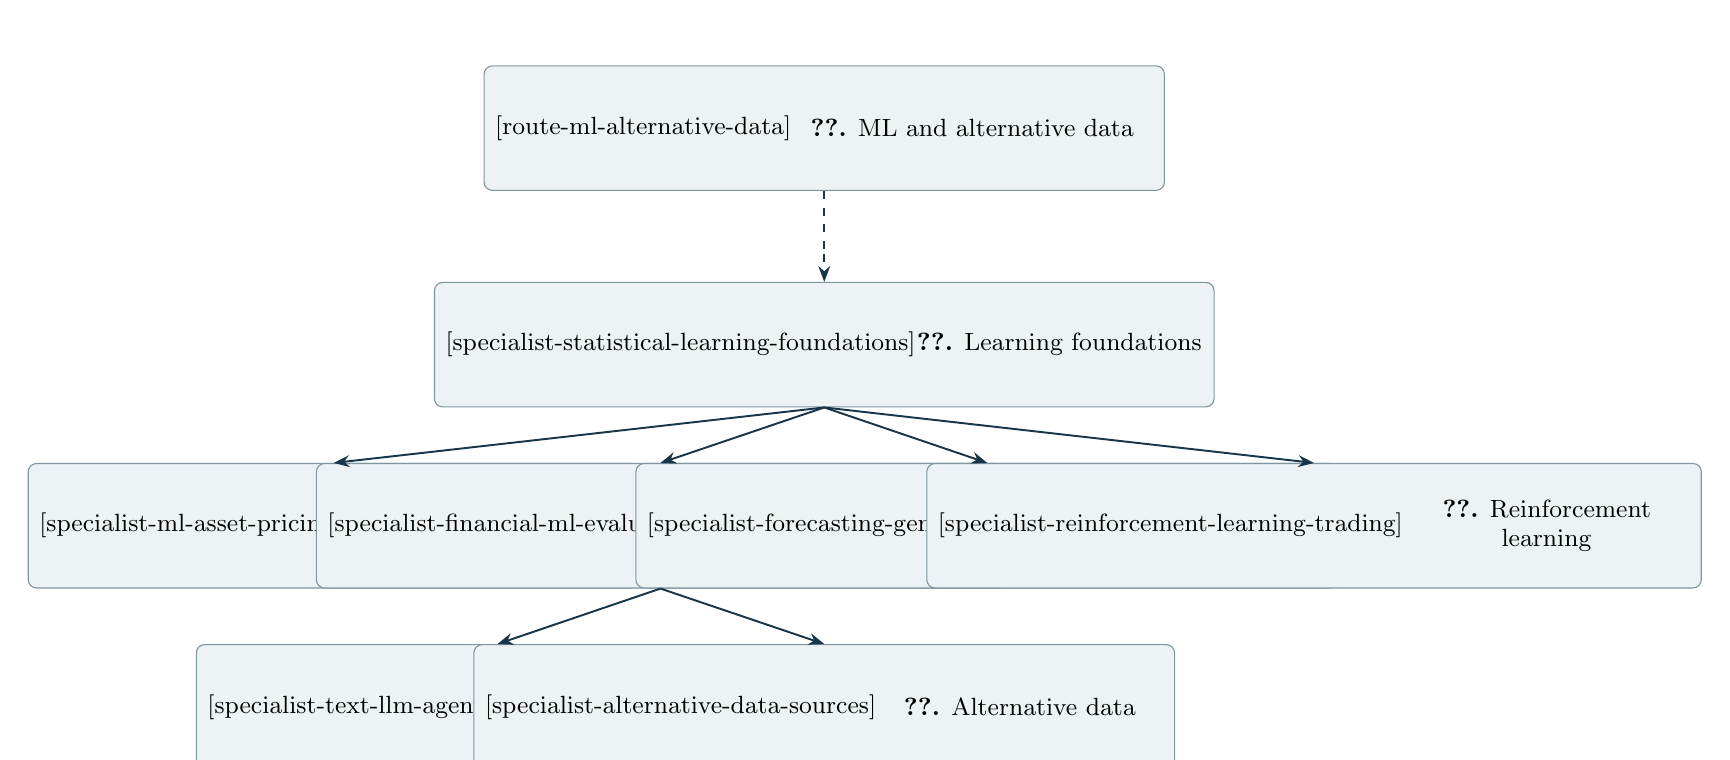
\begin{tikzpicture}[x=1cm,y=1cm]
\node[pathnode] (ml-alternative-data) at (6.23,0) {\MeasurePathNode{4.6cm}{\textbf{\ref*{route-ml-alternative-data}.} ML and alternative data}\hyperref[route-ml-alternative-data]{\parbox[c][\pathnodeheight][c]{4.6cm}{\centering \textbf{\ref*{route-ml-alternative-data}.} ML and alternative data}}};
\node[pathnode] (statistical-learning-foundations) at (6.23,-2.75) {\MeasurePathNode{3.65cm}{\textbf{\ref*{specialist-statistical-learning-foundations}.} Learning foundations}\hyperref[specialist-statistical-learning-foundations]{\parbox[c][\pathnodeheight][c]{3.65cm}{\centering \textbf{\ref*{specialist-statistical-learning-foundations}.} Learning foundations}}};
\node[pathnode] (ml-asset-pricing) at (0.00,-5.05) {\MeasurePathNode{3.65cm}{\textbf{\ref*{specialist-ml-asset-pricing}.} ML asset pricing}\hyperref[specialist-ml-asset-pricing]{\parbox[c][\pathnodeheight][c]{3.65cm}{\centering \textbf{\ref*{specialist-ml-asset-pricing}.} ML asset pricing}}};
\node[pathnode] (financial-ml-evaluation) at (4.15,-5.05) {\MeasurePathNode{3.65cm}{\textbf{\ref*{specialist-financial-ml-evaluation}.} Financial ML: timing, uncertainty and tests}\hyperref[specialist-financial-ml-evaluation]{\parbox[c][\pathnodeheight][c]{3.65cm}{\centering \textbf{\ref*{specialist-financial-ml-evaluation}.} Financial ML: timing, uncertainty and tests}}};
\node[pathnode] (forecasting-generative-rl) at (8.30,-5.05) {\MeasurePathNode{3.65cm}{\textbf{\ref*{specialist-forecasting-generative-rl}.} Deep forecasting and scenarios}\hyperref[specialist-forecasting-generative-rl]{\parbox[c][\pathnodeheight][c]{3.65cm}{\centering \textbf{\ref*{specialist-forecasting-generative-rl}.} Deep forecasting and scenarios}}};
\node[pathnode] (reinforcement-learning-trading) at (12.45,-5.05) {\MeasurePathNode{3.65cm}{\textbf{\ref*{specialist-reinforcement-learning-trading}.} Reinforcement learning}\hyperref[specialist-reinforcement-learning-trading]{\parbox[c][\pathnodeheight][c]{3.65cm}{\centering \textbf{\ref*{specialist-reinforcement-learning-trading}.} Reinforcement learning}}};
\node[pathnode] (text-llm-agents) at (2.08,-7.35) {\MeasurePathNode{3.65cm}{\textbf{\ref*{specialist-text-llm-agents}.} Text, LLMs and agents}\hyperref[specialist-text-llm-agents]{\parbox[c][\pathnodeheight][c]{3.65cm}{\centering \textbf{\ref*{specialist-text-llm-agents}.} Text, LLMs and agents}}};
\node[pathnode] (alternative-data-sources) at (6.23,-7.35) {\MeasurePathNode{3.65cm}{\textbf{\ref*{specialist-alternative-data-sources}.} Alternative data}\hyperref[specialist-alternative-data-sources]{\parbox[c][\pathnodeheight][c]{3.65cm}{\centering \textbf{\ref*{specialist-alternative-data-sources}.} Alternative data}}};
\draw[entryline] (ml-alternative-data.south) -- (6.23,-1.60);
\draw[entryline] (6.23,-1.60) -- (6.23,-1.60);
\draw[entryarrow] (6.23,-1.60) -- (statistical-learning-foundations.north);
\draw[patharrow] (statistical-learning-foundations.south) -- (ml-asset-pricing.north);
\draw[patharrow] (statistical-learning-foundations.south) -- (financial-ml-evaluation.north);
\draw[patharrow] (statistical-learning-foundations.south) -- (forecasting-generative-rl.north);
\draw[patharrow] (statistical-learning-foundations.south) -- (reinforcement-learning-trading.north);
\draw[patharrow] (financial-ml-evaluation.south) -- (text-llm-agents.north);
\draw[patharrow] (financial-ml-evaluation.south) -- (alternative-data-sources.north);
\end{tikzpicture}\end{center}
\textbf{Overview checkpoint.} A section capstone: complete it after \hyperref[specialist-statistical-learning-foundations]{\ref*{specialist-statistical-learning-foundations}} and \hyperref[specialist-financial-ml-evaluation]{\ref*{specialist-financial-ml-evaluation}}.

\textbf{Bring these foundations with you.}\begin{itemize}
\item \hyperref[specialist-empirical-asset-pricing]{Empirical asset pricing: factor models and tests} --- needed by \hyperref[specialist-ml-asset-pricing]{ML asset pricing}.
\item \hyperref[route-common-toolkit]{Common toolkit} --- needed by \hyperref[specialist-financial-ml-evaluation]{Financial ML: timing, uncertainty and tests}.
\item \hyperref[specialist-time-series-volatility]{Time-series econometrics and volatility forecasting} --- needed by \hyperref[specialist-forecasting-generative-rl]{Deep forecasting and scenarios}.
\item \hyperref[specialist-stochastic-calculus-control]{Stochastic calculus and continuous-time control} --- needed by \hyperref[specialist-reinforcement-learning-trading]{Reinforcement learning}.
\end{itemize}\hyperref[learning-map]{Return to the whole-guide DAG.}
\Needspace{12\baselineskip}
\subsection{Statistical learning foundations and time-series validation}\label{specialist-statistical-learning-foundations}
\textbf{Specialist pathway.} In \hyperref[route-ml-alternative-data]{ML and alternative data}.

\textbf{Outcome.} Fit and tune regularised, tree-based and neural models, estimate their out-of-sample error with a validation scheme suited to dependent, non-stationary data, and explain what the model uses.

\textbf{Prerequisites.} The ML and alternative data overview, read for orientation (its checkpoint comes after 4.3); Probability, statistical inference and econometric theory (1.1) helps.

\textbf{Review first.} \hyperref[route-ml-alternative-data]{ML and alternative data}.

\textbf{Required readings, in order}
\begin{enumerate}\raggedright
\Needspace{5\baselineskip}\item \href{institutional_quantitative_finance_reading_list.pdf\#s6-isl}{Gareth James, Daniela Witten, Trevor Hastie and Robert Tibshirani, \emph{An Introduction to Statistical Learning}, 2nd ed.}\CataloguePage{49}\NoteKey{s6-isl}\par \textbf{Foundations.} Learn resampling, regularisation, trees and the bias--variance trade-off with code.
\Needspace{5\baselineskip}\item \href{institutional_quantitative_finance_reading_list.pdf\#s6-esl}{Trevor Hastie, Robert Tibshirani and Jerome Friedman, \emph{The Elements of Statistical Learning}, 2nd ed.}\CataloguePage{49}\NoteKey{s6-esl}\par \textbf{Foundations.} Deepen the same methods with the statistical theory behind them.
\Needspace{5\baselineskip}\item \href{institutional_quantitative_finance_reading_list.pdf\#prob-learning}{Shai Shalev-Shwartz and Shai Ben-David, \emph{Understanding Machine Learning: From Theory to Algorithms}}\CataloguePage{49}\NoteKey{prob-learning}\par \textbf{Theory.} Understand generalisation bounds and why they assume independent samples.
\Needspace{5\baselineskip}\item \href{institutional_quantitative_finance_reading_list.pdf\#catalogue-0736}{Tibshirani (1996), LASSO}\CataloguePage{56}\NoteKey{catalogue-0736}\par \textbf{Methods.} Select and shrink coefficients with the lasso.
\Needspace{5\baselineskip}\item \href{institutional_quantitative_finance_reading_list.pdf\#w5-zou-hastie-enet}{Hui Zou and Trevor Hastie, ``Regularization and variable selection via the elastic net''}\CataloguePage{57}\NoteKey{w5-zou-hastie-enet}\par \textbf{Methods.} Handle correlated predictors with the elastic net.
\Needspace{5\baselineskip}\item \href{institutional_quantitative_finance_reading_list.pdf\#wide-breiman-rf}{Leo Breiman, ``Random Forests''}\CataloguePage{50}\NoteKey{wide-breiman-rf}\par \textbf{Methods.} Average decorrelated trees with random forests.
\Needspace{5\baselineskip}\item \href{institutional_quantitative_finance_reading_list.pdf\#wide-xgboost}{Tianqi Chen and Carlos Guestrin, ``XGBoost: A Scalable Tree Boosting System''}\CataloguePage{50}\NoteKey{wide-xgboost}\par \textbf{Implementation.} Train gradient-boosted trees at scale.
\Needspace{5\baselineskip}\item \href{institutional_quantitative_finance_reading_list.pdf\#wide-grinsztajn-tabular}{Léo Grinsztajn, Edouard Oyallon and Gaël Varoquaux, ``Why do tree-based models still outperform deep learning on typical tabular data?''}\CataloguePage{50}\NoteKey{wide-grinsztajn-tabular}\par \textbf{Evidence.} See why tree ensembles still beat deep networks on most tabular data.
\Needspace{5\baselineskip}\item \href{institutional_quantitative_finance_reading_list.pdf\#wide-prince-udl}{Simon J. D. Prince, \emph{Understanding Deep Learning}}\CataloguePage{50}\NoteKey{wide-prince-udl}\par \textbf{Foundations.} Learn modern deep-learning architectures and training.
\Needspace{5\baselineskip}\item \href{institutional_quantitative_finance_reading_list.pdf\#rf-arlot-celisse-2010}{Sylvain Arlot and Alain Celisse, ``A survey of cross-validation procedures for model selection''}\CataloguePage{51}\NoteKey{rf-arlot-celisse-2010}\par \textbf{Validation.} Choose a cross-validation procedure from its theory, not convention.
\Needspace{5\baselineskip}\item \href{institutional_quantitative_finance_reading_list.pdf\#rf-bergmeir-hyndman-koo-2018}{Christoph Bergmeir, Rob J. Hyndman and Bonsoo Koo, ``A note on the validity of cross-validation for evaluating autoregressive time series prediction''}\CataloguePage{51}\NoteKey{rf-bergmeir-hyndman-koo-2018}\par \textbf{Validation.} Know when k-fold cross-validation is valid for autoregressive forecasting.
\Needspace{5\baselineskip}\item \href{institutional_quantitative_finance_reading_list.pdf\#rf-cerqueira-torgo-mozetic-2020}{Vitor Cerqueira, Luis Torgo and Igor Mozetič, ``Evaluating time series forecasting models: an empirical study on performance estimation methods''}\CataloguePage{51}\NoteKey{rf-cerqueira-torgo-mozetic-2020}\par \textbf{Validation.} Prefer repeated out-of-sample holdouts when series are non-stationary.
\Needspace{5\baselineskip}\item \href{institutional_quantitative_finance_reading_list.pdf\#alpha-afml}{Marcos López de Prado, \emph{Advances in Financial Machine Learning}}\CataloguePage{49}\NoteKey{alpha-afml}\par \textbf{Implementation.} Apply purged and embargoed cross-validation and finance-specific labelling.
\Needspace{5\baselineskip}\item \href{institutional_quantitative_finance_reading_list.pdf\#wide-angelopoulos-bates-conformal}{Anastasios N. Angelopoulos and Stephen Bates, ``Conformal Prediction: A Gentle Introduction''}\CataloguePage{51}\NoteKey{wide-angelopoulos-bates-conformal}\par \textbf{Methods.} Attach distribution-free prediction intervals to any model.
\Needspace{5\baselineskip}\item \href{institutional_quantitative_finance_reading_list.pdf\#catalogue-0730}{Lundberg and Lee (2017), \textquotedblleft A Unified Approach to Interpreting Model Predictions\textquotedblright}\CataloguePage{56}\NoteKey{catalogue-0730}\par \textbf{Methods.} Attribute predictions to features with SHAP.
\Needspace{5\baselineskip}\item \href{institutional_quantitative_finance_reading_list.pdf\#w5-rudin-stop-explaining}{Cynthia Rudin, ``Stop explaining black box machine learning models for high stakes decisions and use interpretable models instead''}\CataloguePage{58}\NoteKey{w5-rudin-stop-explaining}\par \textbf{Counter-evidence.} Weigh inherently interpretable models against post-hoc explanations.
\end{enumerate}
\Needspace{5\baselineskip}\textbf{Checkpoint.} On a monthly stock-characteristic panel, fit ridge, lasso, random forest and gradient boosting. Estimate test error with shuffled k-fold, blocked k-fold, purged-and-embargoed k-fold and rolling-origin validation, and compare each estimate with the error on a final untouched period. Report SHAP importances and conformal interval coverage by year.

\textbf{Optional branches.} \href{institutional_quantitative_finance_reading_list.pdf\#catalogue-0530}{Use the standard deep-learning text.}\BranchPage{50} \href{institutional_quantitative_finance_reading_list.pdf\#wide-bishop-deep-learning}{Study deep learning foundations and concepts.}\BranchPage{50} \href{institutional_quantitative_finance_reading_list.pdf\#catalogue-0529}{Study probabilistic machine learning.}\BranchPage{49} \href{institutional_quantitative_finance_reading_list.pdf\#wide-murphy-advanced}{Go further into probabilistic ML.}\BranchPage{50} \href{institutional_quantitative_finance_reading_list.pdf\#w2-fisher-mcr}{Measure variable importance across the set of good models.}\BranchPage{57} \href{institutional_quantitative_finance_reading_list.pdf\#w5-ribeiro-lime}{Compare local surrogate explanations with SHAP.}\BranchPage{57} \href{institutional_quantitative_finance_reading_list.pdf\#w2-lundberg-treeshap}{Compute exact SHAP values for tree ensembles.}\BranchPage{57}
\par{\small \hyperref[learning-map]{Learning pathway DAG} \textbar{} \hyperref[route-ml-alternative-data]{Section overview} \textbar{} \hyperref[map-ml-alternative-data]{Section DAG}\NoteKey{statistical-learning-foundations}}
\Needspace{12\baselineskip}
\subsection{ML return prediction and asset pricing}\label{specialist-ml-asset-pricing}
\textbf{Specialist pathway.} In \hyperref[route-ml-alternative-data]{ML and alternative data}.

\textbf{Outcome.} Train and evaluate an ML cross-sectional return model against economic restrictions, costs and the complexity debate.

\textbf{Prerequisites.} Statistical learning foundations and time-series validation (4.1); Empirical asset pricing: factor models and tests (2.3).

\textbf{Review first.} \hyperref[route-ml-alternative-data]{ML and alternative data}; \hyperref[specialist-statistical-learning-foundations]{Statistical learning foundations and time-series validation}; \hyperref[specialist-empirical-asset-pricing]{Empirical asset pricing: factor models and tests}.

\textbf{Required readings, in order}
\begin{enumerate}\raggedright
\Needspace{5\baselineskip}\item \href{institutional_quantitative_finance_reading_list.pdf\#wide-kelly-xiu-fml}{Bryan Kelly and Dacheng Xiu, ``Financial Machine Learning''}\CataloguePage{52}\NoteKey{wide-kelly-xiu-fml}\par \textbf{Foundations.} Read the field map of financial machine learning.
\Needspace{5\baselineskip}\item \href{institutional_quantitative_finance_reading_list.pdf\#wide-israel-kelly-moskowitz}{Ronen Israel, Bryan T. Kelly and Tobias J. Moskowitz, ``Can Machines "Learn" Finance?''}\CataloguePage{52}\NoteKey{wide-israel-kelly-moskowitz}\par \textbf{Foundations.} Set expectations for low signal-to-noise prediction.
\Needspace{5\baselineskip}\item \href{institutional_quantitative_finance_reading_list.pdf\#alpha-academicml}{Bryan Kelly, Semyon Malamud and Kangying Zhou, ``The Virtue of Complexity in Return Prediction'', and Shihao Gu, Bryan Kelly and Dacheng Xiu, ``Empirical Asset Pricing via Machine Learning''}\CataloguePage{53}\NoteKey{alpha-academicml}\par \textbf{Evidence.} Study the benchmark ML return-prediction comparison and the complexity argument.
\Needspace{5\baselineskip}\item \href{institutional_quantitative_finance_reading_list.pdf\#wide-fnw-nonparametric}{Joachim Freyberger, Andreas Neuhierl and Michael Weber, ``Dissecting Characteristics Nonparametrically''}\CataloguePage{54}\NoteKey{wide-fnw-nonparametric}\par \textbf{Methods.} Select characteristics nonparametrically.
\Needspace{5\baselineskip}\item \href{institutional_quantitative_finance_reading_list.pdf\#wide-giglio-kelly-xiu-ar}{Stefano Giglio, Bryan Kelly and Dacheng Xiu, ``Factor Models, Machine Learning, and Asset Pricing''}\CataloguePage{52}\NoteKey{wide-giglio-kelly-xiu-ar}\par \textbf{Theory.} Connect ML to factor-model estimation.
\Needspace{5\baselineskip}\item \href{institutional_quantitative_finance_reading_list.pdf\#exp-deep-asset-pricing}{Luyang Chen, Markus Pelger, and Jason Zhu, Deep Learning in Asset Pricing}\CataloguePage{53}\NoteKey{exp-deep-asset-pricing}\par \textbf{Methods.} Estimate an SDF with deep networks and no-arbitrage moments.
\Needspace{5\baselineskip}\item \href{institutional_quantitative_finance_reading_list.pdf\#wide-kmp-principal-portfolios}{Bryan Kelly, Semyon Malamud and Lasse Heje Pedersen, ``Principal Portfolios''}\CataloguePage{54}\NoteKey{wide-kmp-principal-portfolios}\par \textbf{Methods.} Exploit cross-predictability with principal portfolios.
\Needspace{5\baselineskip}\item \href{institutional_quantitative_finance_reading_list.pdf\#exp-seemingly-virtuous-complexity}{Stefan Nagel, Seemingly Virtuous Complexity in Return Prediction}\CataloguePage{54}\NoteKey{exp-seemingly-virtuous-complexity}\par \textbf{Counter-evidence.} Test whether complexity gains are artefacts.
\Needspace{5\baselineskip}\item \href{institutional_quantitative_finance_reading_list.pdf\#wide-didisheim-aipt}{Antoine Didisheim, Shikun (Barry) Ke, Bryan T. Kelly and Semyon Malamud, ``APT or "AIPT"? The Surprising Dominance of Large Factor Models''}\CataloguePage{55}\NoteKey{wide-didisheim-aipt}\par \textbf{Evidence.} Compare large-factor SDF evidence.
\Needspace{5\baselineskip}\item \href{institutional_quantitative_finance_reading_list.pdf\#wide-avramov-cheng-metzker}{Doron Avramov, Si Cheng and Lior Metzker, ``Machine Learning vs. Economic Restrictions: Evidence from Stock Return Predictability''}\CataloguePage{54}\NoteKey{wide-avramov-cheng-metzker}\par \textbf{Counter-evidence.} See how gains shrink under economic restrictions.
\Needspace{5\baselineskip}\item \href{institutional_quantitative_finance_reading_list.pdf\#wide-ml-meets-markowitz}{Yijie Wang, Hao Gao, Campbell R. Harvey, Yan Liu and Xinyuan Tao, ``Machine Learning Meets Markowitz''}\CataloguePage{54}\NoteKey{wide-ml-meets-markowitz}\par \textbf{Implementation.} Train on portfolio objectives rather than return errors.
\end{enumerate}
\Needspace{5\baselineskip}\textbf{Checkpoint.} Fit ridge, gradient-boosted and neural return models on a public characteristics panel with rolling windows; report predictive R2, long-short returns before and after costs and excluding microcaps, and compare a predict-then-optimise portfolio with an end-to-end objective.

\textbf{Optional branches.} \href{institutional_quantitative_finance_reading_list.pdf\#wide-leippold-wang-zhou-china}{Replicate in a retail-dominated market.}\BranchPage{54} \href{institutional_quantitative_finance_reading_list.pdf\#wide-alphaglass}{Compare an interpretable additive-signal portfolio.}\BranchPage{55} \href{institutional_quantitative_finance_reading_list.pdf\#wide-bianchi-bond-ml}{Extend ML prediction to Treasury returns.}\BranchPage{54} \href{institutional_quantitative_finance_reading_list.pdf\#w2-jiang-kelly-xiu-images}{Predict returns from price-chart images.}\BranchPage{55} \href{institutional_quantitative_finance_reading_list.pdf\#w2-candes-knockoffs}{Select features with FDR control.}\BranchPage{57} \href{institutional_quantitative_finance_reading_list.pdf\#w3-cong-panel-trees}{Grow panel trees on the efficient frontier.}\BranchPage{55} \href{institutional_quantitative_finance_reading_list.pdf\#w3-choi-alpha-go}{Train ML market by market internationally.}\BranchPage{56} \href{institutional_quantitative_finance_reading_list.pdf\#w3-allena-confident-premiums}{Trade only precisely forecast stocks.}\BranchPage{55} \href{institutional_quantitative_finance_reading_list.pdf\#w3-li-rossi-yan-universe}{Assess feature engineering versus model choice.}\BranchPage{55} \href{institutional_quantitative_finance_reading_list.pdf\#w4-bai-pukthuanthong-classification}{Compare classification and regression losses for portfolios.}\BranchPage{56} \href{institutional_quantitative_finance_reading_list.pdf\#w4-jo-kim-variable-importance}{Measure variable importance economically, outside microcaps.}\BranchPage{57} \href{institutional_quantitative_finance_reading_list.pdf\#w5-apley-zhu-ale}{Use ALE plots for correlated characteristics.}\BranchPage{57} \href{institutional_quantitative_finance_reading_list.pdf\#w5-friedman-gbm}{Read the gradient-boosting original.}\BranchPage{57} \href{institutional_quantitative_finance_reading_list.pdf\#catalogue-0796}{Model concept-oriented shared information among stocks with a graph network.}\BranchPage{58} \href{institutional_quantitative_finance_reading_list.pdf\#catalogue-0797}{Model cross-stock correlation with a market-guided transformer.}\BranchPage{58} \href{institutional_quantitative_finance_reading_list.pdf\#w2-kipf-welling}{Learn graph convolutional networks.}\BranchPage{59}
\par{\small \hyperref[learning-map]{Learning pathway DAG} \textbar{} \hyperref[route-ml-alternative-data]{Section overview} \textbar{} \hyperref[map-ml-alternative-data]{Section DAG}\NoteKey{ml-asset-pricing}}
\Needspace{12\baselineskip}
\subsection{Financial ML: information timing, uncertainty and portfolio tests}\label{specialist-financial-ml-evaluation}
\textbf{Specialist pathway.} In \hyperref[route-ml-alternative-data]{ML and alternative data}.

\textbf{Outcome.} Assess a modern ML or language-model result using time-valid inputs, numerical checks, appropriate uncertainty and a portfolio decision after implementation costs.

\textbf{Prerequisites.} Statistical learning foundations and time-series validation (4.1); Common toolkit and portfolio-return accounting.

\textbf{Review first.} \hyperref[route-ml-alternative-data]{ML and alternative data}; \hyperref[route-common-toolkit]{Common toolkit}; \hyperref[specialist-statistical-learning-foundations]{Statistical learning foundations and time-series validation}.

\textbf{Required readings, in order}
\begin{enumerate}\raggedright
\Needspace{5\baselineskip}\item \href{institutional_quantitative_finance_reading_list.pdf\#alpha-jansen}{Stefan Jansen, \emph{Machine Learning for Trading}, 3rd ed. (2026); historical second-edition book/code (2020)}\CataloguePage{51}\NoteKey{alpha-jansen}\par \textbf{Workflow.} Use the selected third-edition research workflow; keep historical second-edition examples tied to their own code branch.
\Needspace{5\baselineskip}\item \href{institutional_quantitative_finance_reading_list.pdf\#latest-levy-caution-llm}{Bradford Levy, Caution Ahead: Numerical Reasoning and Look-Ahead Bias in AI Models}\CataloguePage{83}\NoteKey{latest-levy-caution-llm}\par \textbf{Failure modes.} Test numerical operations and training-data look-ahead before interpreting an LLM-derived signal.
\Needspace{5\baselineskip}\item \href{institutional_quantitative_finance_reading_list.pdf\#latest-pit-language-models}{Bryan T. Kelly, Semyon Malamud, Johannes Schwab and Teng Andrea Xu, Scaling Point-in-Time Language Models; Author revision record}\CataloguePage{66}\NoteKey{latest-pit-language-models}\par \textbf{Information sets.} Study model vintages as well as document timestamps when designing a historical text experiment.
\Needspace{5\baselineskip}\item \href{institutional_quantitative_finance_reading_list.pdf\#exp-implementable-frontier}{Theis Ingerslev Jensen, Bryan Kelly, Semyon Malamud, and Lasse Heje Pedersen, Machine Learning and the Implementable Efficient Frontier}\CataloguePage{53}\NoteKey{exp-implementable-frontier}\par \textbf{Economic objective.} Compare candidate models after turnover, trading costs and feasible portfolio constraints.
\Needspace{5\baselineskip}\item \href{institutional_quantitative_finance_reading_list.pdf\#latest-high-dimensional-grs}{Mikhail Chernov, Bryan T. Kelly, Semyon Malamud and Johannes Schwab, A Test of the Efficiency of a Given Portfolio in High Dimensions}\CataloguePage{84}\NoteKey{latest-high-dimensional-grs}\par \textbf{Portfolio validation.} Distinguish a high-dimensional portfolio-efficiency test from model selection, multiple testing and a profitability claim.
\Needspace{5\baselineskip}\item \href{institutional_quantitative_finance_reading_list.pdf\#latest-conformal-time-dependence}{Rina Foygel Barber and Ashwin Pananjady, Predictive inference for time series: why is split conformal effective despite temporal dependence?; January 2026 preprint revision}\CataloguePage{86}\NoteKey{latest-conformal-time-dependence}\par \textbf{Uncertainty.} Identify the dependence and stationarity conditions behind interval coverage instead of importing an exchangeable-data guarantee.
\Needspace{5\baselineskip}\item \href{institutional_quantitative_finance_reading_list.pdf\#latest-bis-market-stress-ml}{Iñaki Aldasoro, Peter Hördahl, Andreas Schrimpf and Xingyu Sonya Zhu, Predicting financial market stress with machine learning}\CataloguePage{41}\NoteKey{latest-bis-market-stress-ml}\par \textbf{Financial target.} Use market-specific stress distributions as an auxiliary forecasting problem with explicit horizons and tail calibration.
\Needspace{5\baselineskip}\item \href{institutional_quantitative_finance_reading_list.pdf\#w5-gneiting-katzfuss}{Tilmann Gneiting and Matthias Katzfuss, ``Probabilistic Forecasting''}\CataloguePage{39}\NoteKey{w5-gneiting-katzfuss}\par \textbf{Validation.} Evaluate probabilistic forecasts by calibration, sharpness and proper scores.
\end{enumerate}
\Needspace{5\baselineskip}\textbf{Checkpoint.} Specify a small time-valid financial-text or market-stress experiment. Record source release times, model-training cutoffs, tuning trials and held-out dates; use code for numerical calculations. Compare a simple baseline with the complex model under the same information set. Report interval coverage by regime and after-cost economic loss, and identify which portfolio-efficiency and dependence assumptions can actually be supported.

\textbf{Optional branches.} \href{institutional_quantitative_finance_reading_list.pdf\#latest-ai-asset-pricing-transformer}{Study transformer-based stochastic-discount-factor pricing after the evaluation controls are specified.}\BranchPage{53} \href{institutional_quantitative_finance_reading_list.pdf\#latest-asset-embeddings}{Compare holdings-based relational features with text and conventional firm characteristics; account for reporting lags.}\BranchPage{58} \href{institutional_quantitative_finance_reading_list.pdf\#latest-complex-modern-portfolio-theory}{Compare recent high-dimensional portfolio claims with the same costs and validation constraints.}\BranchPage{93} \href{institutional_quantitative_finance_reading_list.pdf\#w5-hyndman-koehler}{Choose scale-free point-forecast accuracy measures.}\BranchPage{40} \href{institutional_quantitative_finance_reading_list.pdf\#w5-diebold-gunther-tay}{Test density forecasts with probability integral transforms.}\BranchPage{40} \href{institutional_quantitative_finance_reading_list.pdf\#w5-pesaran-timmermann-sign}{Test directional accuracy of timing signals.}\BranchPage{40} \href{institutional_quantitative_finance_reading_list.pdf\#w5-granger-pesaran-economic}{Judge forecasts by the decisions they support.}\BranchPage{40} \href{institutional_quantitative_finance_reading_list.pdf\#w5-strobl-rf-importance}{Avoid biased impurity-based importance measures.}\BranchPage{58}
\par{\small \hyperref[learning-map]{Learning pathway DAG} \textbar{} \hyperref[route-ml-alternative-data]{Section overview} \textbar{} \hyperref[map-ml-alternative-data]{Section DAG}\NoteKey{financial-ml-evaluation}}
\Needspace{12\baselineskip}
\subsection{Deep forecasting and generative scenarios}\label{specialist-forecasting-generative-rl}
\textbf{Specialist pathway.} In \hyperref[route-ml-alternative-data]{ML and alternative data}.

\textbf{Outcome.} Benchmark deep and foundation forecasters and generate realistic scenarios whose tails, clustering and dependence are checked before use.

\textbf{Prerequisites.} Statistical learning foundations and time-series validation (4.1); Time-series econometrics and volatility forecasting (1.4).

\textbf{Review first.} \hyperref[route-ml-alternative-data]{ML and alternative data}; \hyperref[specialist-statistical-learning-foundations]{Statistical learning foundations and time-series validation}; \hyperref[specialist-time-series-volatility]{Time-series econometrics and volatility forecasting}.

\textbf{Required readings, in order}
\begin{enumerate}\raggedright
\Needspace{5\baselineskip}\item \href{institutional_quantitative_finance_reading_list.pdf\#wide-lim-zohren-survey}{Bryan Lim and Stefan Zohren, ``Time-series forecasting with deep learning: a survey''}\CataloguePage{42}\NoteKey{wide-lim-zohren-survey}\par \textbf{Foundations.} Review deep architectures for forecasting.
\Needspace{5\baselineskip}\item \href{institutional_quantitative_finance_reading_list.pdf\#catalogue-0785}{Bryan Lim et al., ``Temporal Fusion Transformers for Interpretable Multi-horizon Time Series Forecasting''}\CataloguePage{40}\NoteKey{catalogue-0785}\par \textbf{Methods.} Study an interpretable multi-horizon transformer.
\Needspace{5\baselineskip}\item \href{institutional_quantitative_finance_reading_list.pdf\#exp-chronos2}{Abdul Fatir Ansari et al., Chronos-2: From Univariate to Universal Forecasting; Official model repository}\CataloguePage{42}\NoteKey{exp-chronos2}\par \textbf{Methods.} Try a current time-series foundation model.
\Needspace{5\baselineskip}\item \href{institutional_quantitative_finance_reading_list.pdf\#exp-gift-eval}{Taha Aksu, Gerald Woo, Juncheng Liu, Xu Liu, Chenghao Liu, Silvio Savarese, Caiming Xiong and Doyen Sahoo, GIFT-Eval: A Benchmark for General Time Series Forecasting Model Evaluation; official benchmark and change log}\CataloguePage{41}\NoteKey{exp-gift-eval}\par \textbf{Validation.} Use a broad benchmark with leakage controls.
\Needspace{5\baselineskip}\item \href{institutional_quantitative_finance_reading_list.pdf\#wide-kronos}{Yu Shi, Zongliang Fu, Shuo Chen, Bohan Zhao, Wei Xu, Changshui Zhang and Jian Li, ``Kronos: A Foundation Model for the Language of Financial Markets''}\CataloguePage{42}\NoteKey{wide-kronos}\par \textbf{Evidence.} Assess a finance-specific candlestick foundation model.
\Needspace{5\baselineskip}\item \href{institutional_quantitative_finance_reading_list.pdf\#wide-quant-gans}{Magnus Wiese, Robert Knobloch, Ralf Korn and Peter Kretschmer, ``Quant GANs: deep generation of financial time series''}\CataloguePage{70}\NoteKey{wide-quant-gans}\par \textbf{Methods.} Generate scenarios that reproduce stylised facts.
\Needspace{5\baselineskip}\item \href{institutional_quantitative_finance_reading_list.pdf\#wide-lyons-mcleod-signatures}{Terry Lyons and Andrew D. McLeod, ``Signature Methods in Machine Learning''}\CataloguePage{70}\NoteKey{wide-lyons-mcleod-signatures}\par \textbf{Theory.} Represent paths with signatures.
\Needspace{5\baselineskip}\item \href{institutional_quantitative_finance_reading_list.pdf\#wide-buehler-market-generator}{Hans Buehler, Blanka Horvath, Terry Lyons, Imanol Perez Arribas and Ben Wood, ``A Data-driven Market Simulator for Small Data Environments''}\CataloguePage{70}\NoteKey{wide-buehler-market-generator}\par \textbf{Methods.} Generate paths from small data for hedging.
\Needspace{5\baselineskip}\item \href{institutional_quantitative_finance_reading_list.pdf\#exp-nagy-lob-bench}{Peer Nagy et al., LOB-Bench: Benchmarking Generative AI for Finance - an Application to Limit Order Book Data; benchmark project}\CataloguePage{166}\NoteKey{exp-nagy-lob-bench}\par \textbf{Validation.} Evaluate generated order-book data.
\end{enumerate}
\Needspace{5\baselineskip}\textbf{Checkpoint.} Compare a seasonal-naive baseline, HAR, a fine-tuned transformer and a zero-shot foundation model on realised volatility with rolling origins; then generate scenarios with a GAN or signature model and test whether they reproduce tails, clustering and cross-correlations.

\textbf{Optional branches.} \href{institutional_quantitative_finance_reading_list.pdf\#wide-tabpfn}{Test a tabular foundation model on small panels.}\BranchPage{42} \href{institutional_quantitative_finance_reading_list.pdf\#wide-chevyrev-kormilitzin}{Start with a primer on path signatures.}\BranchPage{70}
\par{\small \hyperref[learning-map]{Learning pathway DAG} \textbar{} \hyperref[route-ml-alternative-data]{Section overview} \textbar{} \hyperref[map-ml-alternative-data]{Section DAG}\NoteKey{forecasting-generative-rl}}
\Needspace{12\baselineskip}
\subsection{Reinforcement learning for trading, hedging and execution}\label{specialist-reinforcement-learning-trading}
\textbf{Specialist pathway.} In \hyperref[route-ml-alternative-data]{ML and alternative data}.

\textbf{Outcome.} Formulate a trading, hedging or execution problem as an MDP, train a policy against a validated simulator and compare it with the control-theoretic benchmark.

\textbf{Prerequisites.} Statistical learning foundations and time-series validation (4.1); Stochastic calculus and continuous-time control (1.2).

\textbf{Review first.} \hyperref[route-ml-alternative-data]{ML and alternative data}; \hyperref[specialist-statistical-learning-foundations]{Statistical learning foundations and time-series validation}; \hyperref[specialist-stochastic-calculus-control]{Stochastic calculus and continuous-time control}.

\textbf{Required readings, in order}
\begin{enumerate}\raggedright
\Needspace{5\baselineskip}\item \href{institutional_quantitative_finance_reading_list.pdf\#catalogue-0814}{Sutton and Barto, \emph{Reinforcement Learning}}\CataloguePage{71}\NoteKey{catalogue-0814}\par \textbf{Foundations.} Learn value functions, policy gradients and exploration.
\Needspace{5\baselineskip}\item \href{institutional_quantitative_finance_reading_list.pdf\#wide-hambly-xu-yang}{Ben Hambly, Renyuan Xu and Huining Yang, ``Recent advances in reinforcement learning in finance''}\CataloguePage{71}\NoteKey{wide-hambly-xu-yang}\par \textbf{Foundations.} Survey RL across execution, market making, allocation and hedging.
\Needspace{5\baselineskip}\item \href{institutional_quantitative_finance_reading_list.pdf\#wide-kolm-ritter-rl}{Petter N. Kolm and Gordon Ritter, ``Modern Perspectives on Reinforcement Learning in Finance''}\CataloguePage{71}\NoteKey{wide-kolm-ritter-rl}\par \textbf{Foundations.} Map trading problems to MDPs.
\Needspace{5\baselineskip}\item \href{institutional_quantitative_finance_reading_list.pdf\#wide-wang-zariphopoulou-zhou}{Haoran Wang, Thaleia Zariphopoulou and Xun Yu Zhou, ``Reinforcement Learning in Continuous Time and Space: A Stochastic Control Approach''}\CataloguePage{71}\NoteKey{wide-wang-zariphopoulou-zhou}\par \textbf{Theory.} Connect entropy-regularised exploration with stochastic control.
\Needspace{5\baselineskip}\item \href{institutional_quantitative_finance_reading_list.pdf\#w2-moody-saffell}{John Moody and Matthew Saffell, ``Learning to trade via direct reinforcement''}\CataloguePage{71}\NoteKey{w2-moody-saffell}\par \textbf{Methods.} Optimise a differential Sharpe ratio directly with costs.
\Needspace{5\baselineskip}\item \href{institutional_quantitative_finance_reading_list.pdf\#w2-halperin-qlbs}{Igor Halperin, ``QLBS: Q-Learner in the Black-Scholes(-Merton) Worlds''}\CataloguePage{71}\NoteKey{w2-halperin-qlbs}\par \textbf{Valuation.} Price and hedge options with Q-learning.
\Needspace{5\baselineskip}\item \href{institutional_quantitative_finance_reading_list.pdf\#w2-kolm-ritter-hedging}{Petter N. Kolm and Gordon Ritter, ``Dynamic Replication and Hedging: A Reinforcement Learning Approach''}\CataloguePage{71}\NoteKey{w2-kolm-ritter-hedging}\par \textbf{Implementation.} Hedge with costs using RL.
\Needspace{5\baselineskip}\item \href{institutional_quantitative_finance_reading_list.pdf\#w2-ning-ddqn-execution}{Brian Ning, Franco Ho Ting Lin and Sebastian Jaimungal, ``Double Deep Q-Learning for Optimal Execution''}\CataloguePage{71}\NoteKey{w2-ning-ddqn-execution}\par \textbf{Implementation.} Train a DDQN execution policy against TWAP.
\Needspace{5\baselineskip}\item \href{institutional_quantitative_finance_reading_list.pdf\#wide-spooner-mm-rl}{Thomas Spooner, John Fearnley, Rahul Savani and Andreas Koukorinis, ``Market Making via Reinforcement Learning''}\CataloguePage{163}\NoteKey{wide-spooner-mm-rl}\par \textbf{Implementation.} Train an RL market maker with reward shaping.
\Needspace{5\baselineskip}\item \href{institutional_quantitative_finance_reading_list.pdf\#catalogue-0453}{Hans Buehler, Lukas Gonon, Josef Teichmann and Ben Wood, ``Deep Hedging''}\CataloguePage{127}\NoteKey{catalogue-0453}\par \textbf{Implementation.} Learn deep hedging policies with frictions.
\Needspace{5\baselineskip}\item \href{institutional_quantitative_finance_reading_list.pdf\#w2-finrl}{Xiao-Yang Liu et al., ``FinRL: Deep Reinforcement Learning Framework to Automate Trading in Quantitative Finance''}\CataloguePage{72}\NoteKey{w2-finrl}\par \textbf{Implementation.} Use open environments as experiment scaffolding, not evidence.
\Needspace{5\baselineskip}\item \href{institutional_quantitative_finance_reading_list.pdf\#w4-brini-kolm-ppo-trading}{Alessio Brini and Petter N. Kolm, ``On Deep Reinforcement Learning for Dynamic Trading with PPO: Challenges and Future Directions''}\CataloguePage{72}\NoteKey{w4-brini-kolm-ppo-trading}\par \textbf{Validation.} Benchmark PPO against a known optimal trading policy.
\end{enumerate}
\Needspace{5\baselineskip}\textbf{Checkpoint.} Train an RL execution or hedging policy in a simulator calibrated to real data; compare with Almgren--Chriss or delta hedging on cost and risk, report seeds, hyperparameter trials and out-of-sample degradation when the simulator is perturbed.

\textbf{Optional branches.} \href{institutional_quantitative_finance_reading_list.pdf\#section.3.7}{Browse the reinforcement-learning section.}\BranchPage{71} \href{institutional_quantitative_finance_reading_list.pdf\#wide-gasperov-mm-review}{Review RL market-making evaluation weaknesses.}\BranchPage{164} \href{institutional_quantitative_finance_reading_list.pdf\#w3-gao-li-zhou-rl-jumps}{Extend continuous-time RL to jumps.}\BranchPage{72} \href{institutional_quantitative_finance_reading_list.pdf\#w3-cheridito-weiss-rl-execution}{Allocate market and limit orders with RL.}\BranchPage{72} \href{institutional_quantitative_finance_reading_list.pdf\#w4-wang-gao-li-rl-execution}{Use continuous-time actor-critic RL for execution.}\BranchPage{72} \href{institutional_quantitative_finance_reading_list.pdf\#w4-jha-rl-saa-objective}{See the objective dominate RL allocation results.}\BranchPage{72} \href{institutional_quantitative_finance_reading_list.pdf\#w4-corimayo-rl-derivatives-review}{Survey RL for derivatives pricing and hedging.}\BranchPage{72}
\par{\small \hyperref[learning-map]{Learning pathway DAG} \textbar{} \hyperref[route-ml-alternative-data]{Section overview} \textbar{} \hyperref[map-ml-alternative-data]{Section DAG}\NoteKey{reinforcement-learning-trading}}
\Needspace{12\baselineskip}
\subsection{Text, language models and agent evaluation}\label{specialist-text-llm-agents}
\textbf{Specialist pathway.} In \hyperref[route-ml-alternative-data]{ML and alternative data}.

\textbf{Outcome.} Build a time-valid text signal, measure look-ahead contamination and evaluate LLM or agent strategies over long samples.

\textbf{Prerequisites.} Financial ML: information timing, uncertainty and portfolio tests (4.3).

\textbf{Review first.} \hyperref[route-ml-alternative-data]{ML and alternative data}; \hyperref[specialist-financial-ml-evaluation]{Financial ML: information timing, uncertainty and portfolio tests}.

\textbf{Required readings, in order}
\begin{enumerate}\raggedright
\Needspace{5\baselineskip}\item \href{institutional_quantitative_finance_reading_list.pdf\#wide-gentzkow-kelly-taddy}{Matthew Gentzkow, Bryan Kelly and Matt Taddy, ``Text as Data''}\CataloguePage{64}\NoteKey{wide-gentzkow-kelly-taddy}\par \textbf{Foundations.} Survey text representations and their economic uses.
\Needspace{5\baselineskip}\item \href{institutional_quantitative_finance_reading_list.pdf\#exp-loughran-mcdonald}{Tim Loughran and Bill McDonald, When Is a Liability Not a Liability? Textual Analysis, Dictionaries, and 10-Ks}\CataloguePage{64}\NoteKey{exp-loughran-mcdonald}\par \textbf{Methods.} Use finance-specific dictionaries as a baseline.
\Needspace{5\baselineskip}\item \href{institutional_quantitative_finance_reading_list.pdf\#wide-ke-kelly-xiu-sestm}{Zheng Tracy Ke, Bryan T. Kelly and Dacheng Xiu, ``Predicting Returns with Text Data''}\CataloguePage{64}\NoteKey{wide-ke-kelly-xiu-sestm}\par \textbf{Methods.} Fit a supervised, transparent text model.
\Needspace{5\baselineskip}\item \href{institutional_quantitative_finance_reading_list.pdf\#wide-bybee-business-news}{Leland Bybee, Bryan Kelly, Asaf Manela and Dacheng Xiu, ``Business News and Business Cycles''}\CataloguePage{64}\NoteKey{wide-bybee-business-news}\par \textbf{Evidence.} Measure economic attention from news topics.
\Needspace{5\baselineskip}\item \href{institutional_quantitative_finance_reading_list.pdf\#wide-lopez-lira-tang}{Alejandro Lopez-Lira and Yuehua Tang, ``Can ChatGPT Forecast Stock Price Movements? Return Predictability and Large Language Models''}\CataloguePage{67}\NoteKey{wide-lopez-lira-tang}\par \textbf{Evidence.} Study LLM headline scores and return prediction.
\Needspace{5\baselineskip}\item \href{institutional_quantitative_finance_reading_list.pdf\#wide-chen-kelly-xiu-llm}{Yifei Chen, Bryan T. Kelly and Dacheng Xiu, ``Expected Returns and Large Language Models''}\CataloguePage{67}\NoteKey{wide-chen-kelly-xiu-llm}\par \textbf{Evidence.} Compare embeddings across models and markets.
\Needspace{5\baselineskip}\item \href{institutional_quantitative_finance_reading_list.pdf\#wide-glasserman-lin-lookahead}{Paul Glasserman and Caden Lin, ``Assessing Look-Ahead Bias in Stock Return Predictions Generated by GPT Sentiment Analysis''}\CataloguePage{67}\NoteKey{wide-glasserman-lin-lookahead}\par \textbf{Validation.} Separate look-ahead from distraction by anonymisation.
\Needspace{5\baselineskip}\item \href{institutional_quantitative_finance_reading_list.pdf\#wide-sarkar-vafa-lookahead}{Suproteem K. Sarkar and Keyon Vafa, ``Lookahead Bias in Pretrained Language Models''}\CataloguePage{67}\NoteKey{wide-sarkar-vafa-lookahead}\par \textbf{Validation.} Test pretrained models for post-period knowledge.
\Needspace{5\baselineskip}\item \href{institutional_quantitative_finance_reading_list.pdf\#wide-chrono-llm}{Songrun He, Linying Lv, Asaf Manela and Jimmy Wu, ``Chronologically Consistent Large Language Models''}\CataloguePage{67}\NoteKey{wide-chrono-llm}\par \textbf{Methods.} Use chronologically consistent models.
\Needspace{5\baselineskip}\item \href{institutional_quantitative_finance_reading_list.pdf\#wide-finqa}{Zhiyu Chen et al., ``FinQA: A Dataset of Numerical Reasoning over Financial Data''}\CataloguePage{67}\NoteKey{wide-finqa}\par \textbf{Validation.} Benchmark numerical reasoning.
\Needspace{5\baselineskip}\item \href{institutional_quantitative_finance_reading_list.pdf\#wide-finsaber}{Weixian Waylon Li, Hyeonjun Kim, Mihai Cucuringu and Tiejun Ma, ``Can LLM-based Financial Investing Strategies Outperform the Market in Long Run?''}\CataloguePage{68}\NoteKey{wide-finsaber}\par \textbf{Counter-evidence.} See LLM strategy gains fade in long backtests.
\Needspace{5\baselineskip}\item \href{institutional_quantitative_finance_reading_list.pdf\#wide-koijen-levy-agentic}{Ralph S. J. Koijen and Bradford Levy, ``Assessing the Benefits of Optimized Agentic AI Systems for Asset Pricing''}\CataloguePage{68}\NoteKey{wide-koijen-levy-agentic}\par \textbf{Evidence.} Evaluate agentic systems in real time without look-ahead.
\Needspace{5\baselineskip}\item \href{institutional_quantitative_finance_reading_list.pdf\#w2-stockbench}{Authors as listed on arXiv (StockBench), ``StockBench: Can LLM Agents Trade Stocks Profitably In Real-world Markets?''}\CataloguePage{68}\NoteKey{w2-stockbench}\par \textbf{Validation.} Use a contamination-free trading benchmark.
\Needspace{5\baselineskip}\item \href{institutional_quantitative_finance_reading_list.pdf\#w2-livetradebench}{Authors as listed on arXiv (LiveTradeBench, UIUC), ``LiveTradeBench: Seeking Real-World Alpha with Large Language Models''}\CataloguePage{68}\NoteKey{w2-livetradebench}\par \textbf{Validation.} Evaluate agents live without backtest leakage.
\Needspace{5\baselineskip}\item \href{institutional_quantitative_finance_reading_list.pdf\#w5-loughran-mcdonald-survey}{Tim Loughran and Bill McDonald, ``Textual Analysis in Accounting and Finance: A Survey''}\CataloguePage{64}\NoteKey{w5-loughran-mcdonald-survey}\par \textbf{Foundations.} Learn dictionary, readability and similarity methods for financial text.
\end{enumerate}
\Needspace{5\baselineskip}\textbf{Checkpoint.} Score five years of headlines with a dictionary, SESTM and a chronologically consistent LLM; report returns by sample period relative to each model's training cutoff, anonymised versus named inputs, and results after costs over the longest available history.

\textbf{Optional branches.} \href{institutional_quantitative_finance_reading_list.pdf\#wide-tradingagents}{Inspect a multi-agent trading architecture as a design reference.}\BranchPage{68} \href{institutional_quantitative_finance_reading_list.pdf\#wide-kim-muhn-nikolaev}{Test LLM financial-statement analysis claims.}\BranchPage{67} \href{institutional_quantitative_finance_reading_list.pdf\#wide-financebench}{Benchmark retrieval over filings.}\BranchPage{67} \href{institutional_quantitative_finance_reading_list.pdf\#w3-sheng-genai-asset-management}{Study hedge-fund GenAI adoption and returns.}\BranchPage{68} \href{institutional_quantitative_finance_reading_list.pdf\#w3-eisfeldt-genai-firm-values}{Price firm exposure to generative AI.}\BranchPage{68} \href{institutional_quantitative_finance_reading_list.pdf\#w4-kim-llm-correlations}{Use LLM-derived relationships in correlation estimates.}\BranchPage{68} \href{institutional_quantitative_finance_reading_list.pdf\#w5-cohen-malloy-nguyen-lazy-prices}{Trade on changes in filing language.}\BranchPage{65} \href{institutional_quantitative_finance_reading_list.pdf\#w5-hoberg-phillips-tnic}{Build text-based industry peers.}\BranchPage{65} \href{institutional_quantitative_finance_reading_list.pdf\#w5-tetlock-saar-macskassy}{Measure fundamentals from news tone.}\BranchPage{64} \href{institutional_quantitative_finance_reading_list.pdf\#w5-hassan-political-risk}{Measure firm-level risks from earnings calls.}\BranchPage{65} \href{institutional_quantitative_finance_reading_list.pdf\#rf-cong-liang-zhang-zhu-2025}{Build interpretable textual factors from embeddings and topic models.}\BranchPage{65}
\par{\small \hyperref[learning-map]{Learning pathway DAG} \textbar{} \hyperref[route-ml-alternative-data]{Section overview} \textbar{} \hyperref[map-ml-alternative-data]{Section DAG}\NoteKey{text-llm-agents}}
\Needspace{12\baselineskip}
\subsection{Alternative data: sources, information value and market effects}\label{specialist-alternative-data-sources}
\textbf{Specialist pathway.} In \hyperref[route-ml-alternative-data]{ML and alternative data}.

\textbf{Outcome.} Assess an alternative dataset by its coverage, timing and incremental information over consensus, test its return and fundamentals predictability, and judge how its edge decays as access spreads.

\textbf{Prerequisites.} Financial ML: information timing, uncertainty and portfolio tests (4.3); Point-in-time data (3.2) for vendor histories. Event studies (2.7) helps.

\textbf{Review first.} \hyperref[route-ml-alternative-data]{ML and alternative data}; \hyperref[specialist-financial-ml-evaluation]{Financial ML: information timing, uncertainty and portfolio tests}.

\textbf{Required readings, in order}
\begin{enumerate}\raggedright
\Needspace{5\baselineskip}\item \href{institutional_quantitative_finance_reading_list.pdf\#wide-kolanovic-big-data}{Marko Kolanovic and Rajesh T. Krishnamachari, ``Big Data and AI Strategies: Machine Learning and Alternative Data Approach to Investing''}\CataloguePage{61}\NoteKey{wide-kolanovic-big-data}\par \textbf{Foundations.} Use a practitioner taxonomy of alternative-data sources and methods.
\Needspace{5\baselineskip}\item \href{institutional_quantitative_finance_reading_list.pdf\#rf-monk-prins-rook-2019}{Ashby Monk, Marcel Prins and Dane Rook, ``Rethinking Alternative Data in Institutional Investment''}\CataloguePage{62}\NoteKey{rf-monk-prins-rook-2019}\par \textbf{Foundations.} Decide which datasets fit an institution's resources and strategy.
\Needspace{5\baselineskip}\item \href{institutional_quantitative_finance_reading_list.pdf\#rf-froot-kang-ozik-sadka-2017}{Kenneth Froot, Namho Kang, Gideon Ozik and Ronnie Sadka, ``What do measures of real-time corporate sales say about earnings surprises and post-announcement returns?''}\CataloguePage{62}\NoteKey{rf-froot-kang-ozik-sadka-2017}\par \textbf{Evidence.} Predict sales and earnings surprises from real-time mobile-device data.
\Needspace{5\baselineskip}\item \href{institutional_quantitative_finance_reading_list.pdf\#rf-dichev-qian-2022}{Ilia D. Dichev and Jingyi Qian, ``The benefits of transaction-level data: The case of NielsenIQ scanner data''}\CataloguePage{63}\NoteKey{rf-dichev-qian-2022}\par \textbf{Evidence.} Predict revenue and returns from retail scanner data.
\Needspace{5\baselineskip}\item \href{institutional_quantitative_finance_reading_list.pdf\#rf-kang-stice-lawrence-wong-2021}{Jung Koo Kang, Lorien Stice-Lawrence and Yu Ting Forester Wong, ``The Firm Next Door: Using Satellite Images to Study Local Information Advantage''}\CataloguePage{62}\NoteKey{rf-kang-stice-lawrence-wong-2021}\par \textbf{Evidence.} Measure store-level performance from satellite car counts.
\Needspace{5\baselineskip}\item \href{institutional_quantitative_finance_reading_list.pdf\#rf-katona-painter-patatoukas-zeng-2025}{Zsolt Katona, Marcus O. Painter, Panos N. Patatoukas and Jean Zeng, ``On the Capital Market Consequences of Big Data: Evidence from Outer Space''}\CataloguePage{62}\NoteKey{rf-katona-painter-patatoukas-zeng-2025}\par \textbf{Evidence.} See unequal access to satellite data raise information asymmetry.
\Needspace{5\baselineskip}\item \href{institutional_quantitative_finance_reading_list.pdf\#exp-altdata-governance}{Christina Zhu, Big Data as a Governance Mechanism}\CataloguePage{61}\NoteKey{exp-altdata-governance}\par \textbf{Evidence.} See alternative-data coverage change price informativeness and managerial behaviour.
\Needspace{5\baselineskip}\item \href{institutional_quantitative_finance_reading_list.pdf\#wide-green-employer-reviews}{T. Clifton Green, Ruoyan Huang, Quan Wen and Dexin Zhou, ``Crowdsourced employer reviews and stock returns''}\CataloguePage{61}\NoteKey{wide-green-employer-reviews}\par \textbf{Evidence.} Build a crowd-sourced employee-review signal.
\Needspace{5\baselineskip}\item \href{institutional_quantitative_finance_reading_list.pdf\#rf-chen-de-hu-hwang-2014}{Hailiang Chen, Prabuddha De, Yu (Jeffrey) Hu and Byoung-Hyoun Hwang, ``Wisdom of Crowds: The Value of Stock Opinions Transmitted Through Social Media''}\CataloguePage{63}\NoteKey{rf-chen-de-hu-hwang-2014}\par \textbf{Evidence.} Extract return information from investor social media.
\Needspace{5\baselineskip}\item \href{institutional_quantitative_finance_reading_list.pdf\#eq-da-engelberg-gao-2011}{Zhi Da, Joseph Engelberg and Pengjie Gao, ``In Search of Attention''}\CataloguePage{206}\NoteKey{eq-da-engelberg-gao-2011}\par \textbf{Evidence.} Measure investor attention from search volume.
\Needspace{5\baselineskip}\item \href{institutional_quantitative_finance_reading_list.pdf\#rf-grennan-michaely-2021}{Jillian Grennan and Roni Michaely, ``FinTechs and the Market for Financial Analysis''}\CataloguePage{63}\NoteKey{rf-grennan-michaely-2021}\par \textbf{Evidence.} See how data aggregators synthesise non-traditional sources.
\Needspace{5\baselineskip}\item \href{institutional_quantitative_finance_reading_list.pdf\#rf-dessaint-foucault-fresard-2024}{Olivier Dessaint, Thierry Foucault and Laurent Frésard, ``Does Alternative Data Improve Financial Forecasting? The Horizon Effect''}\CataloguePage{63}\NoteKey{rf-dessaint-foucault-fresard-2024}\par \textbf{Counter-evidence.} Check whether short-horizon data crowd out long-horizon forecasting.
\Needspace{5\baselineskip}\item \href{institutional_quantitative_finance_reading_list.pdf\#exp-financial-data-value}{Maryam Farboodi, Dhruv Singal, Laura Veldkamp, and Venky Venkateswaran, Valuing Financial Data}\CataloguePage{61}\NoteKey{exp-financial-data-value}\par \textbf{Valuation.} Value a dataset by its contribution to a specific portfolio.
\Needspace{5\baselineskip}\item \href{institutional_quantitative_finance_reading_list.pdf\#rf-farboodi-veldkamp-2020}{Maryam Farboodi and Laura Veldkamp, ``Long-Run Growth of Financial Data Technology''}\CataloguePage{63}\NoteKey{rf-farboodi-veldkamp-2020}\par \textbf{Theory.} Model the long-run shift between fundamental and order-flow data.
\end{enumerate}
\Needspace{5\baselineskip}\textbf{Checkpoint.} For a set of listed retailers, join one alternative sales proxy (card panel, web traffic, foot traffic or car counts) with documented coverage start dates and release lags. Test whether it predicts revenue surprises and announcement returns beyond analyst consensus, in a point-in-time panel, and compare the effect before and after the data became widely sold.

\textbf{Optional branches.} \href{institutional_quantitative_finance_reading_list.pdf\#wide-huang-customer-knows}{Use customer product ratings as a signal.}\BranchPage{61} \href{institutional_quantitative_finance_reading_list.pdf\#w3-xue-thermal-satellite}{Track factory activity with thermal satellite imagery.}\BranchPage{62} \href{institutional_quantitative_finance_reading_list.pdf\#w3-lieberman-b2b-payments}{Use business-to-business payment timeliness.}\BranchPage{62} \href{institutional_quantitative_finance_reading_list.pdf\#wide-mukherjee-satellite}{Measure oil inventories from satellite images.}\BranchPage{61} \href{institutional_quantitative_finance_reading_list.pdf\#rf-begenau-farboodi-veldkamp-2018}{Link big-data coverage to firm size and the cost of capital.}\BranchPage{63} \href{institutional_quantitative_finance_reading_list.pdf\#rf-abis-veldkamp-2024}{Estimate how data change knowledge production in asset management.}\BranchPage{63} \href{institutional_quantitative_finance_reading_list.pdf\#alpha-aima}{Read an industry survey of alternative-data adoption.}\BranchPage{60} \href{institutional_quantitative_finance_reading_list.pdf\#w2-menzly-ozbas}{Trade on supplier and customer links.}\BranchPage{59} \href{institutional_quantitative_finance_reading_list.pdf\#wide-lee-tech-links}{Build technology-link signals from patents.}\BranchPage{59}
\par{\small \hyperref[learning-map]{Learning pathway DAG} \textbar{} \hyperref[route-ml-alternative-data]{Section overview} \textbar{} \hyperref[map-ml-alternative-data]{Section DAG}\NoteKey{alternative-data-sources}}
\clearpage
\part{Public markets and pricing}\label{part-public-markets}
Progress from securities and derivatives to cross-asset, currency, international equity and regional market decisions.

\textbf{Sections in learning order}\begin{enumerate}
\item[\ref*{route-rates-credit-mortgages}.] \hyperref[route-rates-credit-mortgages]{Rates: yield curves, term premia and derivatives} --- Build curves and rate-derivative conventions, then read monetary policy and term premia in the curve, forecast bond excess returns and price inflation-linked claims.
\item[\ref*{route-government-bond-markets}.] \hyperref[route-government-bond-markets]{Government bond markets and sovereign debt} --- Study Treasury market structure and issuance, sovereign default and restructuring, and municipal bonds; then compare euro-area, UK and Japanese markets with the Treasury market.
\item[\ref*{route-corporate-credit-capital}.] \hyperref[route-corporate-credit-capital]{Corporate credit, hybrids and labelled bonds} --- Model default and recovery, reconcile bond spreads with CDS, then study subordinated bank and corporate hybrids and sustainability-labelled bonds.
\item[\ref*{route-securitised-structured-credit}.] \hyperref[route-securitised-structured-credit]{Securitised and structured credit} --- Compare dual-recourse and asset-based structures, then model mortgage, ABS and CLO cash flows and synthetic risk transfer; CMBS builds on the mortgage, ABS and CLO waterfalls.
\item[\ref*{route-systematic-equities}.] \hyperref[route-systematic-equities]{Systematic equities} --- Start from factor premia, statistical arbitrage, investor flows and fundamental valuation; then study short-selling, option, insider and retail-flow signals, combine signals into a risk-controlled long–short portfolio, and finish with corporate events and merger arbitrage.
\item[\ref*{route-volatility-options}.] \hyperref[route-volatility-options]{Option pricing, volatility models and hedging} --- Start with stochastic, local and jump models, or with convertibles, a separate entry point; then rough and path-dependent volatility and the hedges each model implies, learned pricing, and exotics and structured products. Volatility trading and option premia are in the next section; crypto options appear with digital assets.
\item[\ref*{route-volatility-trading-premia}.] \hyperref[route-volatility-trading-premia]{Volatility trading, option premia and implied information} --- Start with index option returns, variance premia and dealer hedging and with option-implied densities and tail risk; continue to single-stock option returns, VIX, correlation and dividend claims, and short-dated and retail option trading. Options market making is in Part III.
\item[\ref*{route-multi-asset-systematic-macro}.] \hyperref[route-multi-asset-systematic-macro]{Multi-asset and systematic macro} --- Start with cross-asset style premia, trend following, risk parity and macro announcements; macro regimes and the stock–bond correlation build on risk parity, and nowcasting builds on announcements. Currencies follow in their own section.
\item[\ref*{route-currency-markets}.] \hyperref[route-currency-markets]{Currency markets: exchange rates, premia and hedging} --- Start with exchange-rate determination and with FX forwards, options, fixes and settlement. Currency premia build on determination, and covered interest parity and dollar funding on the instruments; continue to FX volatility and crash risk, then currency hedging and emerging-market currencies and intervention, which draw on both premia and funding. FX dealing is in Part III.
\item[\ref*{route-international-equity-markets}.] \hyperref[route-international-equity-markets]{International and emerging equity markets} --- Start with integration, diversification and home bias. Global factors, emerging and frontier markets, and cross-listings build on it, and the China pathway draws on global factors and emerging-market evidence. Capital flows, local-currency bonds and market access follow in the next section.
\item[\ref*{route-global-regional-markets}.] \hyperref[route-global-regional-markets]{Global and regional markets: capital flows, local bonds and market access} --- Start with capital flows and benchmark-driven investors, then local-currency government bonds, then trace a security through access, custody, settlement, tax and hedging. Equity integration, emerging-market equities and China are in the previous section.
\end{enumerate}
\hyperref[learning-map]{Return to the learning pathway DAG.}
\clearpage
\section{Rates: yield curves, term premia and derivatives}\label{route-rates-credit-mortgages}
\label{route-4}
\textbf{Learning sequence.} Build curves and rate-derivative conventions, then read monetary policy and term premia in the curve, forecast bond excess returns and price inflation-linked claims.

\textbf{Section goals.} Across its pathways, this section teaches you to:
\begin{itemize}[leftmargin=1.4em,itemsep=0pt,topsep=1pt]
\item build zero curves and estimate and compare affine term-structure models (\hyperref[specialist-curve-term-structure]{\ref*{specialist-curve-term-structure}})
\item price caps, swaptions and SOFR futures with calibrated models and risk-free-rate conventions (\hyperref[specialist-rate-derivatives]{\ref*{specialist-rate-derivatives}})
\item read the expected policy path and separate policy, term-premium and balance-sheet channels (\hyperref[specialist-monetary-policy-curve]{\ref*{specialist-monetary-policy-curve}})
\item forecast bond excess returns and build systematic rates signals (\hyperref[specialist-bond-risk-premia]{\ref*{specialist-bond-risk-premia}})
\item price inflation-linked bonds and swaps and decompose breakevens (\hyperref[specialist-rates-inflation]{\ref*{specialist-rates-inflation}})
\end{itemize}
\textbf{Overview outcome.} Connect a rate quote or bond position to its curve, expected policy path, term premium, collateral and hedge-contract assumptions.

\textbf{Prerequisites.} Common toolkit; discount factors, bond cash flows, swaps and futures.

\textbf{Review first.} \hyperref[route-common-toolkit]{Common toolkit}.

\textbf{Required readings, in order}
\begin{enumerate}\raggedright
\Needspace{5\baselineskip}\item \href{institutional_quantitative_finance_reading_list.pdf\#rt-gurkaynak-wright-2012}{Refet S. Gürkaynak and Jonathan H. Wright, ``Macroeconomics and the Term Structure''}\CataloguePage{216}\NoteKey{rt-gurkaynak-wright-2012}\par Frame the yield curve through expected policy, time-varying term premia and macroeconomic news.
\Needspace{5\baselineskip}\item \href{institutional_quantitative_finance_reading_list.pdf\#s6-brigo}{Damiano Brigo and Fabio Mercurio, \emph{Interest Rate Models: Theory and Practice}}\CataloguePage{213}\NoteKey{s6-brigo}\par Establish arbitrage-consistent term-structure modelling and rate-derivative notation.
\Needspace{5\baselineskip}\item \href{institutional_quantitative_finance_reading_list.pdf\#exp-adrian-crump-moench-term-structure}{Tobias Adrian, Richard K. Crump, and Emanuel Moench, Pricing the Term Structure with Linear Regressions; New York Fed ACM term-premium data notes}\CataloguePage{214}\NoteKey{exp-adrian-crump-moench-term-structure}\par Use an empirical decomposition to distinguish expected policy from estimated term premium.
\Needspace{5\baselineskip}\item \href{institutional_quantitative_finance_reading_list.pdf\#gap-rates-sofr-futures-hedging}{CME Group, Pricing and Hedging USD SOFR Interest Rate Swaps with SOFR Futures}\CataloguePage{224}\NoteKey{gap-rates-sofr-futures-hedging}\par Tie a modern overnight-rate curve and swap hedge to exchange-traded contract conventions.
\Needspace{5\baselineskip}\item \href{institutional_quantitative_finance_reading_list.pdf\#gap-gregory5}{Jon Gregory, The xVA Challenge: A Valuation Adjustment Framework for Modern Derivatives Markets}\CataloguePage{182}\NoteKey{gap-gregory5}\par Close the valuation loop with collateral, counterparty exposure, funding, margin and capital, using the July 2026 fifth edition.
\end{enumerate}
\Needspace{5\baselineskip}\textbf{Checkpoint.} Build a cash-flow and risk-assumption sheet for one collateralised swap hedged with SOFR futures and one Treasury note. Reprice both under level and slope moves, a policy-path surprise, a term-premium shock and a collateral or funding change; identify assumptions that cannot all hold together.

\textbf{Optional branches.} \href{institutional_quantitative_finance_reading_list.pdf\#section.11.5}{Extend the curve and cash-flow framework to inflation indexation.}\BranchPage{226} \href{institutional_quantitative_finance_reading_list.pdf\#s6-xva}{Compare the retained historical third edition of the xVA text.}\BranchPage{181}
\par\textbf{Continue in this section.} \hyperref[specialist-curve-term-structure]{Yield-curve construction and term-structure models}; \hyperref[specialist-rate-derivatives]{Interest-rate derivatives, volatility and RFR conventions}; \hyperref[specialist-monetary-policy-curve]{Monetary policy, balance-sheet policy and the yield curve}; \hyperref[specialist-bond-risk-premia]{Bond risk premia, predictability and systematic rates strategies}; \hyperref[specialist-rates-inflation]{Inflation-linked bonds, real yields and breakevens}.
\par{\small \hyperref[learning-map]{Learning pathway DAG} \textbar{} \hyperref[map-rates-credit-mortgages]{Section DAG}\NoteKey{rates-credit-mortgages}}
\clearpage
\subsection*{Rates: yield curves, term premia and derivatives: pathway DAG}\phantomsection\label{map-rates-credit-mortgages}
\addcontentsline{toc}{subsection}{Rates: yield curves, term premia and derivatives: pathway DAG}
Start with the section overview's readings, for orientation. Solid arrows show prerequisites within this section. Dashed connectors identify entry points with no further prerequisite in this section; the linked foundations below still apply. Follow the arrows for dependencies and the subsection numbers for reading order. Every node is clickable.
\begin{center}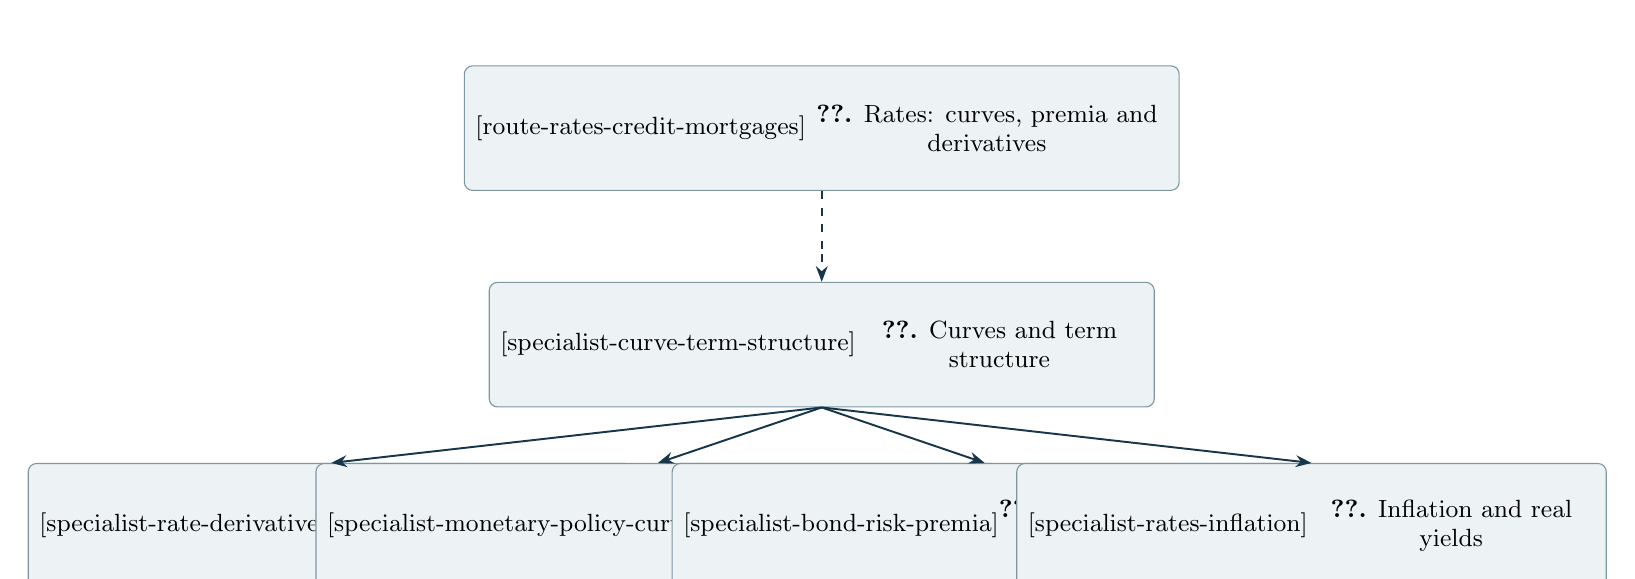
\begin{tikzpicture}[x=1cm,y=1cm]
\node[pathnode] (rates-credit-mortgages) at (6.23,0) {\MeasurePathNode{4.6cm}{\textbf{\ref*{route-rates-credit-mortgages}.} Rates: curves, premia and derivatives}\hyperref[route-rates-credit-mortgages]{\parbox[c][\pathnodeheight][c]{4.6cm}{\centering \textbf{\ref*{route-rates-credit-mortgages}.} Rates: curves, premia and derivatives}}};
\node[pathnode] (curve-term-structure) at (6.23,-2.75) {\MeasurePathNode{3.65cm}{\textbf{\ref*{specialist-curve-term-structure}.} Curves and term structure}\hyperref[specialist-curve-term-structure]{\parbox[c][\pathnodeheight][c]{3.65cm}{\centering \textbf{\ref*{specialist-curve-term-structure}.} Curves and term structure}}};
\node[pathnode] (rate-derivatives) at (0.00,-5.05) {\MeasurePathNode{3.65cm}{\textbf{\ref*{specialist-rate-derivatives}.} Rate derivatives}\hyperref[specialist-rate-derivatives]{\parbox[c][\pathnodeheight][c]{3.65cm}{\centering \textbf{\ref*{specialist-rate-derivatives}.} Rate derivatives}}};
\node[pathnode] (monetary-policy-curve) at (4.15,-5.05) {\MeasurePathNode{3.65cm}{\textbf{\ref*{specialist-monetary-policy-curve}.} Policy and the curve}\hyperref[specialist-monetary-policy-curve]{\parbox[c][\pathnodeheight][c]{3.65cm}{\centering \textbf{\ref*{specialist-monetary-policy-curve}.} Policy and the curve}}};
\node[pathnode] (bond-risk-premia) at (8.30,-5.05) {\MeasurePathNode{3.65cm}{\textbf{\ref*{specialist-bond-risk-premia}.} Bond risk premia and strategies}\hyperref[specialist-bond-risk-premia]{\parbox[c][\pathnodeheight][c]{3.65cm}{\centering \textbf{\ref*{specialist-bond-risk-premia}.} Bond risk premia and strategies}}};
\node[pathnode] (rates-inflation) at (12.45,-5.05) {\MeasurePathNode{3.65cm}{\textbf{\ref*{specialist-rates-inflation}.} Inflation and real yields}\hyperref[specialist-rates-inflation]{\parbox[c][\pathnodeheight][c]{3.65cm}{\centering \textbf{\ref*{specialist-rates-inflation}.} Inflation and real yields}}};
\draw[entryline] (rates-credit-mortgages.south) -- (6.23,-1.60);
\draw[entryline] (6.23,-1.60) -- (6.23,-1.60);
\draw[entryarrow] (6.23,-1.60) -- (curve-term-structure.north);
\draw[patharrow] (curve-term-structure.south) -- (rate-derivatives.north);
\draw[patharrow] (curve-term-structure.south) -- (monetary-policy-curve.north);
\draw[patharrow] (curve-term-structure.south) -- (bond-risk-premia.north);
\draw[patharrow] (curve-term-structure.south) -- (rates-inflation.north);
\end{tikzpicture}\end{center}
\textbf{Bring these foundations with you.}\begin{itemize}
\item \hyperref[specialist-stochastic-calculus-control]{Stochastic calculus and continuous-time control} --- needed by \hyperref[specialist-rate-derivatives]{Rate derivatives}.
\item \hyperref[specialist-return-predictability]{Return predictability and forecast evaluation} --- needed by \hyperref[specialist-bond-risk-premia]{Bond risk premia and strategies}.
\end{itemize}\hyperref[learning-map]{Return to the whole-guide DAG.}
\Needspace{12\baselineskip}
\subsection{Yield-curve construction and term-structure models}\label{specialist-curve-term-structure}
\textbf{Specialist pathway.} In \hyperref[route-rates-credit-mortgages]{Rates: yield curves, term premia and derivatives}.

\textbf{Outcome.} Build a zero curve, decompose yields into expectations and term premia, and estimate and compare affine term-structure models.

\textbf{Prerequisites.} Rates overview; stochastic calculus basics.

\textbf{Review first.} \hyperref[route-rates-credit-mortgages]{Rates: yield curves, term premia and derivatives}.

\textbf{Required readings, in order}
\begin{enumerate}\raggedright
\Needspace{5\baselineskip}\item \href{institutional_quantitative_finance_reading_list.pdf\#catalogue-0233}{Bruce Tuckman and Angel Serrat, \emph{Fixed Income Securities: Tools for Today's Markets}, fourth edition}\CataloguePage{212}\NoteKey{catalogue-0233}\par \textbf{Mechanics.} Review bond math, curves and hedging.
\Needspace{5\baselineskip}\item \href{institutional_quantitative_finance_reading_list.pdf\#wide-litterman-scheinkman}{Robert Litterman and José Scheinkman, ``Common Factors Affecting Bond Returns''}\CataloguePage{213}\NoteKey{wide-litterman-scheinkman}\par \textbf{Evidence.} Identify level, slope and curvature.
\Needspace{5\baselineskip}\item \href{institutional_quantitative_finance_reading_list.pdf\#wide-nelson-siegel}{Charles R. Nelson and Andrew F. Siegel, ``Parsimonious Modeling of Yield Curves''}\CataloguePage{212}\NoteKey{wide-nelson-siegel}\par \textbf{Methods.} Fit a parsimonious curve.
\Needspace{5\baselineskip}\item \href{institutional_quantitative_finance_reading_list.pdf\#wide-hagan-west-interp}{Patrick S. Hagan and Graeme West, ``Interpolation Methods for Curve Construction''}\CataloguePage{212}\NoteKey{wide-hagan-west-interp}\par \textbf{Implementation.} Choose an interpolation with stable forwards.
\Needspace{5\baselineskip}\item \href{institutional_quantitative_finance_reading_list.pdf\#wide-ametrano-bianchetti}{Ferdinando M. Ametrano and Marco Bianchetti, ``Everything You Always Wanted to Know About Multiple Interest Rate Curve Bootstrapping but Were Afraid to Ask''}\CataloguePage{212}\NoteKey{wide-ametrano-bianchetti}\par \textbf{Implementation.} Bootstrap multi-curve OIS and tenor curves.
\Needspace{5\baselineskip}\item \href{institutional_quantitative_finance_reading_list.pdf\#wide-gsw-yield-curve}{Refet S. Gürkaynak, Brian Sack and Jonathan H. Wright, ``The U.S. Treasury yield curve: 1961 to the present''}\CataloguePage{213}\NoteKey{wide-gsw-yield-curve}\par \textbf{Data.} Use the Fed zero-coupon curve and its construction.
\Needspace{5\baselineskip}\item \href{institutional_quantitative_finance_reading_list.pdf\#wide-diebold-li}{Francis X. Diebold and Canlin Li, ``Forecasting the term structure of government bond yields''}\CataloguePage{212}\NoteKey{wide-diebold-li}\par \textbf{Methods.} Forecast with dynamic Nelson--Siegel factors.
\Needspace{5\baselineskip}\item \href{institutional_quantitative_finance_reading_list.pdf\#s6-vasicek}{Oldrich Vasicek, ``An Equilibrium Characterization of the Term Structure''}\CataloguePage{214}\NoteKey{s6-vasicek}\par \textbf{Theory.} Start from a one-factor equilibrium model.
\Needspace{5\baselineskip}\item \href{institutional_quantitative_finance_reading_list.pdf\#wide-cir-1985}{John C. Cox, Jonathan E. Ingersoll Jr. and Stephen A. Ross, ``A Theory of the Term Structure of Interest Rates''}\CataloguePage{214}\NoteKey{wide-cir-1985}\par \textbf{Theory.} Keep rates non-negative with square-root dynamics.
\Needspace{5\baselineskip}\item \href{institutional_quantitative_finance_reading_list.pdf\#wide-hull-white}{John Hull and Alan White, ``Pricing Interest-Rate-Derivative Securities''}\CataloguePage{215}\NoteKey{wide-hull-white}\par \textbf{Valuation.} Fit the initial curve exactly.
\Needspace{5\baselineskip}\item \href{institutional_quantitative_finance_reading_list.pdf\#s6-hjm}{David Heath, Robert Jarrow and Andrew Morton, ``Bond Pricing and the Term Structure of Interest Rates: A New Methodology for Contingent Claims Valuation''}\CataloguePage{214}\NoteKey{s6-hjm}\par \textbf{Theory.} Derive the no-arbitrage drift of forward-rate dynamics.
\Needspace{5\baselineskip}\item \href{institutional_quantitative_finance_reading_list.pdf\#wide-duffee-essentially}{Gregory R. Duffee, ``Term Premia and Interest Rate Forecasts in Affine Models''}\CataloguePage{215}\NoteKey{wide-duffee-essentially}\par \textbf{Theory.} Allow time-varying risk premia.
\Needspace{5\baselineskip}\item \href{institutional_quantitative_finance_reading_list.pdf\#wide-jsz}{Scott Joslin, Kenneth J. Singleton and Haoxiang Zhu, ``A New Perspective on Gaussian Dynamic Term Structure Models''}\CataloguePage{215}\NoteKey{wide-jsz}\par \textbf{Methods.} Estimate Gaussian dynamic term-structure models efficiently.
\Needspace{5\baselineskip}\item \href{institutional_quantitative_finance_reading_list.pdf\#rt-cdr-afns-2011}{Jens H. E. Christensen, Francis X. Diebold and Glenn D. Rudebusch, ``The affine arbitrage-free class of Nelson--Siegel term structure models''}\CataloguePage{216}\NoteKey{rt-cdr-afns-2011}\par \textbf{Methods.} Impose no-arbitrage on the Nelson--Siegel factors.
\Needspace{5\baselineskip}\item \href{institutional_quantitative_finance_reading_list.pdf\#exp-adrian-crump-moench-term-structure}{Tobias Adrian, Richard K. Crump, and Emanuel Moench, Pricing the Term Structure with Linear Regressions; New York Fed ACM term-premium data notes}\CataloguePage{214}\NoteKey{exp-adrian-crump-moench-term-structure}\par \textbf{Evidence.} Use regression-based term-premium estimates.
\Needspace{5\baselineskip}\item \href{institutional_quantitative_finance_reading_list.pdf\#rt-kim-wright-2005}{Don H. Kim and Jonathan H. Wright, ``An Arbitrage-Free Three-Factor Term Structure Model and the Recent Behavior of Long-Term Yields and Distant-Horizon Forward Rates''}\CataloguePage{216}\NoteKey{rt-kim-wright-2005}\par \textbf{Evidence.} Compare the Kim--Wright term premium with the ACM estimate.
\end{enumerate}
\Needspace{5\baselineskip}\textbf{Checkpoint.} Bootstrap a Treasury zero curve with two interpolation methods and compare forward-rate smoothness; estimate a three-factor Gaussian ATSM and its arbitrage-free Nelson--Siegel restriction, decompose the ten-year yield into expectations and term premium, and compare with the ACM and Kim--Wright series.

\textbf{Optional branches.} \href{institutional_quantitative_finance_reading_list.pdf\#wide-rebonato-bond-pricing}{Read a structural treatment of yields and convexity.}\BranchPage{213} \href{institutional_quantitative_finance_reading_list.pdf\#wide-liu-wu-yield-curve}{Compare a kernel-smoothed curve dataset.}\BranchPage{213} \href{institutional_quantitative_finance_reading_list.pdf\#wide-huggins-schaller}{Turn curve tools into relative-value trades.}\BranchPage{213} \href{institutional_quantitative_finance_reading_list.pdf\#w4-filipovic-pelger-shrinking-ts}{Estimate smooth investable term-structure factors.}\BranchPage{216} \href{institutional_quantitative_finance_reading_list.pdf\#wide-dai-singleton}{Classify affine models by their admissible factor dynamics.}\BranchPage{215} \href{institutional_quantitative_finance_reading_list.pdf\#exp-kiley-quasi-real-time-term-premium}{Re-estimate term premia in quasi-real time.}\BranchPage{214}
\par{\small \hyperref[learning-map]{Learning pathway DAG} \textbar{} \hyperref[route-rates-credit-mortgages]{Section overview} \textbar{} \hyperref[map-rates-credit-mortgages]{Section DAG}\NoteKey{curve-term-structure}}
\Needspace{12\baselineskip}
\subsection{Interest-rate derivatives, volatility and RFR conventions}\label{specialist-rate-derivatives}
\textbf{Specialist pathway.} In \hyperref[route-rates-credit-mortgages]{Rates: yield curves, term premia and derivatives}.

\textbf{Outcome.} Price caps, swaptions and SOFR futures with a calibrated model and explain smile, convexity and convention effects.

\textbf{Prerequisites.} Curve construction and stochastic calculus.

\textbf{Review first.} \hyperref[specialist-curve-term-structure]{Yield-curve construction and term-structure models}; \hyperref[specialist-stochastic-calculus-control]{Stochastic calculus and continuous-time control}.

\textbf{Required readings, in order}
\begin{enumerate}\raggedright
\Needspace{5\baselineskip}\item \href{institutional_quantitative_finance_reading_list.pdf\#s6-brigo}{Damiano Brigo and Fabio Mercurio, \emph{Interest Rate Models: Theory and Practice}}\CataloguePage{213}\NoteKey{s6-brigo}\par \textbf{Valuation.} Learn short-rate and market models for rate options.
\Needspace{5\baselineskip}\item \href{institutional_quantitative_finance_reading_list.pdf\#wide-bgm-lmm}{Alan Brace, Dariusz Gatarek and Marek Musiela, ``The Market Model of Interest Rate Dynamics''}\CataloguePage{225}\NoteKey{wide-bgm-lmm}\par \textbf{Theory.} Derive the market model consistent with Black prices.
\Needspace{5\baselineskip}\item \href{institutional_quantitative_finance_reading_list.pdf\#rt-lss-2001}{Francis A. Longstaff, Pedro Santa-Clara and Eduardo S. Schwartz, ``The Relative Valuation of Caps and Swaptions: Theory and Empirical Evidence''}\CataloguePage{226}\NoteKey{rt-lss-2001}\par \textbf{Evidence.} Back out swaption-implied correlations and test caps against them.
\Needspace{5\baselineskip}\item \href{institutional_quantitative_finance_reading_list.pdf\#wide-hagan-sabr}{Patrick S. Hagan, Deep Kumar, Andrew S. Lesniewski and Diana E. Woodward, ``Managing Smile Risk''}\CataloguePage{119}\NoteKey{wide-hagan-sabr}\par \textbf{Valuation.} Fit the SABR smile and know its low-strike issues.
\Needspace{5\baselineskip}\item \href{institutional_quantitative_finance_reading_list.pdf\#rt-arbitrage-free-sabr-2014}{Patrick S. Hagan, Deep Kumar, Andrew Lesniewski and Diana Woodward, ``Arbitrage-Free SABR''}\CataloguePage{226}\NoteKey{rt-arbitrage-free-sabr-2014}\par \textbf{Implementation.} Remove low-strike arbitrage from the SABR expansion.
\Needspace{5\baselineskip}\item \href{institutional_quantitative_finance_reading_list.pdf\#gap-rates-multicurve-sabr}{Marco Bianchetti and Mattia Carlicchi, Interest Rates After the Credit Crunch: Multiple-Curve Vanilla Derivatives and SABR}\CataloguePage{224}\NoteKey{gap-rates-multicurve-sabr}\par \textbf{Implementation.} Apply SABR in a multi-curve setting.
\Needspace{5\baselineskip}\item \href{institutional_quantitative_finance_reading_list.pdf\#wide-trolle-schwartz-usv}{Anders B. Trolle and Eduardo S. Schwartz, ``A General Stochastic Volatility Model for the Pricing of Interest Rate Derivatives''}\CataloguePage{225}\NoteKey{wide-trolle-schwartz-usv}\par \textbf{Evidence.} Model unspanned volatility in caps and swaptions.
\Needspace{5\baselineskip}\item \href{institutional_quantitative_finance_reading_list.pdf\#rt-cdg-usv-2002}{Pierre Collin-Dufresne and Robert S. Goldstein, ``Do Bonds Span the Fixed Income Markets? Theory and Evidence for Unspanned Stochastic Volatility''}\CataloguePage{226}\NoteKey{rt-cdg-usv-2002}\par \textbf{Evidence.} Test whether bonds span volatility risk.
\Needspace{5\baselineskip}\item \href{institutional_quantitative_finance_reading_list.pdf\#rt-hanson-convexity-2014}{Samuel G. Hanson, ``Mortgage convexity''}\CataloguePage{226}\NoteKey{rt-hanson-convexity-2014}\par \textbf{Evidence.} Trace how MBS convexity hedging moves rate premia and volatility.
\Needspace{5\baselineskip}\item \href{institutional_quantitative_finance_reading_list.pdf\#rt-schrimpf-sushko-rfr-2019}{Andreas Schrimpf and Vladyslav Sushko, ``Beyond LIBOR: a primer on the new benchmark rates''}\CataloguePage{225}\NoteKey{rt-schrimpf-sushko-rfr-2019}\par \textbf{Mechanics.} Explain why overnight risk-free rates replaced IBORs.
\Needspace{5\baselineskip}\item \href{institutional_quantitative_finance_reading_list.pdf\#gap-rates-backward-term-rates}{Andrei Lyashenko and Fabio Mercurio, Looking Forward to Backward-Looking Rates: A Modeling Framework for Term Rates Replacing LIBOR}\CataloguePage{224}\NoteKey{gap-rates-backward-term-rates}\par \textbf{Mechanics.} Model backward-looking RFR term rates.
\Needspace{5\baselineskip}\item \href{institutional_quantitative_finance_reading_list.pdf\#exp-sofr-data}{Federal Reserve Bank of New York, Additional Information about Reference Rates Administered by the New York Fed; SOFR averages and index; 2024 methodology change}\CataloguePage{517}\NoteKey{exp-sofr-data}\par \textbf{Data.} Pin SOFR observations, calculation conventions and release timing.
\Needspace{5\baselineskip}\item \href{institutional_quantitative_finance_reading_list.pdf\#wide-mercurio-sofr}{Fabio Mercurio, ``A Simple Multi-Curve Model for Pricing SOFR Futures and Other Derivatives''}\CataloguePage{225}\NoteKey{wide-mercurio-sofr}\par \textbf{Valuation.} Price SOFR futures convexity.
\Needspace{5\baselineskip}\item \href{institutional_quantitative_finance_reading_list.pdf\#wide-skov-skovmand-sofr}{Jacob Bjerre Skov and David Skovmand, ``Dynamic term structure models for SOFR futures''}\CataloguePage{225}\NoteKey{wide-skov-skovmand-sofr}\par \textbf{Evidence.} Estimate term-structure models on SOFR futures.
\Needspace{5\baselineskip}\item \href{institutional_quantitative_finance_reading_list.pdf\#gap-rates-isda-definitions}{International Swaps and Derivatives Association, 2021 ISDA Interest Rate Derivatives Definitions; ISDA 2021 Definitions InfoHub}\CataloguePage{224}\NoteKey{gap-rates-isda-definitions}\par \textbf{Mechanics.} Pin contract terms in the 2021 ISDA definitions.
\Needspace{5\baselineskip}\item \href{institutional_quantitative_finance_reading_list.pdf\#catalogue-0235}{Leif Andersen and Vladimir Piterbarg, \emph{Interest Rate Modeling}}\CataloguePage{213}\NoteKey{catalogue-0235}\par \textbf{Valuation.} Use the practitioner reference for calibration and exotic rates.
\end{enumerate}
\Needspace{5\baselineskip}\textbf{Checkpoint.} Calibrate SABR to one swaption expiry across strikes, check the implied density at low strikes against the arbitrage-free variant, and calibrate a Hull--White model to the co-terminal swaptions; price a Bermudan swaption both ways, compare cap prices with swaption-implied correlations, and compute the SOFR futures convexity adjustment implied by your short-rate model.

\textbf{Optional branches.} \href{institutional_quantitative_finance_reading_list.pdf\#wide-henrard-multicurve}{Go deeper into multi-curve implementation.}\BranchPage{212} \href{institutional_quantitative_finance_reading_list.pdf\#catalogue-0926}{Use rateslib for curve and swap calculations.}\BranchPage{523} \href{institutional_quantitative_finance_reading_list.pdf\#w3-bickersteth-sofr-derivatives}{Price and hedge SOFR derivatives.}\BranchPage{225} \href{institutional_quantitative_finance_reading_list.pdf\#w3-klingler-syrstad-sofr}{Compare SOFR and LIBOR floating-rate notes.}\BranchPage{225} \href{institutional_quantitative_finance_reading_list.pdf\#w4-ding-rutkowski-ccbs}{Price RFR cross-currency basis swaps.}\BranchPage{225} \href{institutional_quantitative_finance_reading_list.pdf\#w4-pennanen-sofr-statistical}{Simulate SOFR with a statistical term-structure model.}\BranchPage{225} \href{institutional_quantitative_finance_reading_list.pdf\#rt-andersen-benzoni-2010}{Test term-structure models with realised yield volatility.}\BranchPage{226} \href{institutional_quantitative_finance_reading_list.pdf\#rt-cmv-bond-vrp-2017}{Replicate Treasury variance swaps and their premium.}\BranchPage{226}
\par{\small \hyperref[learning-map]{Learning pathway DAG} \textbar{} \hyperref[route-rates-credit-mortgages]{Section overview} \textbar{} \hyperref[map-rates-credit-mortgages]{Section DAG}\NoteKey{rate-derivatives}}
\Needspace{12\baselineskip}
\subsection{Monetary policy, balance-sheet policy and the yield curve}\label{specialist-monetary-policy-curve}
\textbf{Specialist pathway.} In \hyperref[route-rates-credit-mortgages]{Rates: yield curves, term premia and derivatives}.

\textbf{Outcome.} Read the expected policy path from futures, measure policy surprises at high frequency, and separate rate-path, term-premium and balance-sheet channels in long yields.

\textbf{Prerequisites.} Yield-curve construction and term-structure models; event-study regression.

\textbf{Review first.} \hyperref[specialist-curve-term-structure]{Yield-curve construction and term-structure models}.

\textbf{Required readings, in order}
\begin{enumerate}\raggedright
\Needspace{5\baselineskip}\item \href{institutional_quantitative_finance_reading_list.pdf\#rt-kuttner-2001}{Kenneth N. Kuttner, ``Monetary policy surprises and interest rates: Evidence from the Fed funds futures market''}\CataloguePage{220}\NoteKey{rt-kuttner-2001}\par \textbf{Mechanics.} Extract the surprise component of a policy decision from fed funds futures.
\Needspace{5\baselineskip}\item \href{institutional_quantitative_finance_reading_list.pdf\#rt-piazzesi-swanson-2008}{Monika Piazzesi and Eric T. Swanson, ``Futures prices as risk-adjusted forecasts of monetary policy''}\CataloguePage{220}\NoteKey{rt-piazzesi-swanson-2008}\par \textbf{Evidence.} Adjust futures-implied policy paths for risk premia.
\Needspace{5\baselineskip}\item \href{institutional_quantitative_finance_reading_list.pdf\#wide-gss-policy}{Refet S. Gürkaynak, Brian Sack and Eric T. Swanson, ``Do Actions Speak Louder Than Words? The Response of Asset Prices to Monetary Policy Actions and Statements''}\CataloguePage{271}\NoteKey{wide-gss-policy}\par \textbf{Evidence.} Separate target and path factors in FOMC announcements.
\Needspace{5\baselineskip}\item \href{institutional_quantitative_finance_reading_list.pdf\#rt-hanson-stein-2015}{Samuel G. Hanson and Jeremy C. Stein, ``Monetary policy and long-term real rates''}\CataloguePage{220}\NoteKey{rt-hanson-stein-2015}\par \textbf{Evidence.} Test why policy news moves distant real forwards.
\Needspace{5\baselineskip}\item \href{institutional_quantitative_finance_reading_list.pdf\#rt-hanson-lucca-wright-2021}{Samuel G. Hanson, David O. Lucca and Jonathan H. Wright, ``Rate-Amplifying Demand and the Excess Sensitivity of Long-Term Rates''}\CataloguePage{221}\NoteKey{rt-hanson-lucca-wright-2021}\par \textbf{Evidence.} Link the excess sensitivity of long rates to rate-amplifying demand.
\Needspace{5\baselineskip}\item \href{institutional_quantitative_finance_reading_list.pdf\#rt-swanson-2021}{Eric T. Swanson, ``Measuring the effects of federal reserve forward guidance and asset purchases on financial markets''}\CataloguePage{221}\NoteKey{rt-swanson-2021}\par \textbf{Evidence.} Identify forward-guidance and asset-purchase factors at the lower bound.
\Needspace{5\baselineskip}\item \href{institutional_quantitative_finance_reading_list.pdf\#wide-vayanos-vila}{Dimitri Vayanos and Jean-Luc Vila, ``A Preferred-Habitat Model of the Term Structure of Interest Rates''}\CataloguePage{215}\NoteKey{wide-vayanos-vila}\par \textbf{Theory.} Model how purchases change term premia through preferred habitat and arbitrageur risk.
\Needspace{5\baselineskip}\item \href{institutional_quantitative_finance_reading_list.pdf\#rt-gagnon-lsap-2011}{Joseph Gagnon, Matthew Raskin, Julie Remache and Brian Sack, ``The Financial Market Effects of the Federal Reserve's Large-Scale Asset Purchases''}\CataloguePage{221}\NoteKey{rt-gagnon-lsap-2011}\par \textbf{Evidence.} Read the event-study evidence on the Fed's 2008--10 purchases.
\Needspace{5\baselineskip}\item \href{institutional_quantitative_finance_reading_list.pdf\#rt-kvj-qe-2011}{Arvind Krishnamurthy and Annette Vissing-Jorgensen, ``The Effects of Quantitative Easing on Interest Rates: Channels and Implications for Policy''}\CataloguePage{221}\NoteKey{rt-kvj-qe-2011}\par \textbf{Evidence.} Separate the signalling, safety, duration and credit channels of QE.
\Needspace{5\baselineskip}\item \href{institutional_quantitative_finance_reading_list.pdf\#rt-damico-king-2013}{Stefania D'Amico and Thomas B. King, ``Flow and stock effects of large-scale treasury purchases: Evidence on the importance of local supply''}\CataloguePage{221}\NoteKey{rt-damico-king-2013}\par \textbf{Evidence.} Measure stock and flow effects of purchases security by security.
\Needspace{5\baselineskip}\item \href{institutional_quantitative_finance_reading_list.pdf\#rt-wu-xia-2016}{Jing Cynthia Wu and Fan Dora Xia, ``Measuring the Macroeconomic Impact of Monetary Policy at the Zero Lower Bound''}\CataloguePage{221}\NoteKey{rt-wu-xia-2016}\par \textbf{Methods.} Summarise lower-bound policy with a shadow rate and its model dependence.
\Needspace{5\baselineskip}\item \href{institutional_quantitative_finance_reading_list.pdf\#rt-du-forbes-luzzetti-2024}{Wenxin Du, Kristin Forbes and Matthew N. Luzzetti, ``Quantitative Tightening Around the Globe: What Have We Learned?''}\CataloguePage{222}\NoteKey{rt-du-forbes-luzzetti-2024}\par \textbf{Evidence.} Compare QT announcement effects across seven central banks.
\Needspace{5\baselineskip}\item \href{institutional_quantitative_finance_reading_list.pdf\#rt-fed-balance-sheet-2025}{Board of Governors of the Federal Reserve System, Implementation Note issued October 29, 2025; Roberto Perli, Eric LeSueur and Linsey Molloy, Federal Reserve Bank of New York, The Implementation of Reserve Management Purchases to Maintain Ample Reserves}\CataloguePage{222}\NoteKey{rt-fed-balance-sheet-2025}\par \textbf{Regulation.} Date the end of Fed runoff and the start of bill purchases.
\Needspace{5\baselineskip}\item \href{institutional_quantitative_finance_reading_list.pdf\#latest-ashtari-tafti-liquidity-policy-2025}{Oliver Ashtari-Tafti, Rodrigo Guimaraes, Gábor Pintér and Jean-Charles Wijnandts, The Liquidity State Dependence of Monetary Policy Transmission}\CataloguePage{218}\NoteKey{latest-ashtari-tafti-liquidity-policy-2025}\par \textbf{Evidence.} Allow policy transmission to vary with Treasury market liquidity.
\Needspace{5\baselineskip}\item \href{institutional_quantitative_finance_reading_list.pdf\#rt-bauer-rudebusch-2020}{Michael D. Bauer and Glenn D. Rudebusch, ``Interest Rates under Falling Stars''}\CataloguePage{222}\NoteKey{rt-bauer-rudebusch-2020}\par \textbf{Evidence.} Separate trend r* and inflation from term premia in long yields.
\end{enumerate}
\Needspace{5\baselineskip}\textbf{Checkpoint.} Build an FOMC event study: compute fed funds or SOFR futures surprises in a 30-minute window, regress two- and ten-year Treasury yield and ACM term-premium changes on target and path factors, and add one QE and one QT announcement. Report how much of each long-yield move is expected path and how much term premium, and show where the split depends on the model or window.

\textbf{Optional branches.} \href{institutional_quantitative_finance_reading_list.pdf\#wide-nakamura-steinsson}{Separate policy news from the information effect.}\BranchPage{271} \href{institutional_quantitative_finance_reading_list.pdf\#wide-bauer-swanson}{Remove predictable components from policy surprises.}\BranchPage{271} \href{institutional_quantitative_finance_reading_list.pdf\#rt-altavilla-2019}{Use the euro-area policy-surprise database.}\BranchPage{222} \href{institutional_quantitative_finance_reading_list.pdf\#rt-hlw-2017}{Estimate the natural rate across four economies.}\BranchPage{221} \href{institutional_quantitative_finance_reading_list.pdf\#exp-gourinchas-ray-vayanos-preferred-habitat}{Extend preferred habitat to two countries and exchange rates.}\BranchPage{214} \href{institutional_quantitative_finance_reading_list.pdf\#exp-cordes-infante-repo-issuance-qt}{Trace QT and issuance into repo rates.}\BranchPage{177}
\par{\small \hyperref[learning-map]{Learning pathway DAG} \textbar{} \hyperref[route-rates-credit-mortgages]{Section overview} \textbar{} \hyperref[map-rates-credit-mortgages]{Section DAG}\NoteKey{monetary-policy-curve}}
\Needspace{12\baselineskip}
\subsection{Bond risk premia, predictability and systematic rates strategies}\label{specialist-bond-risk-premia}
\textbf{Specialist pathway.} In \hyperref[route-rates-credit-mortgages]{Rates: yield curves, term premia and derivatives}.

\textbf{Outcome.} Forecast bond excess returns out of sample, judge their economic value after real-time data, small-sample bias and costs, and build carry, value and momentum signals for government-bond futures.

\textbf{Prerequisites.} Yield-curve construction and term-structure models; return predictability and forecast evaluation.

\textbf{Review first.} \hyperref[specialist-curve-term-structure]{Yield-curve construction and term-structure models}; \hyperref[specialist-return-predictability]{Return predictability and forecast evaluation}.

\textbf{Required readings, in order}
\begin{enumerate}\raggedright
\Needspace{5\baselineskip}\item \href{institutional_quantitative_finance_reading_list.pdf\#s16-r32}{Eugene F. Fama and Robert R. Bliss, \emph{The Information in Long-Maturity Forward Rates}, \emph{American Economic Review} (1987); John Y. Campbell and Robert J. Shiller, \emph{Yield Spreads and Interest Rate Movements: A Bird\textquotesingle s Eye View} (1991)}\CataloguePage{214}\NoteKey{s16-r32}\par \textbf{Evidence.} Start from forward-spread and yield-spread forecasts of excess returns.
\Needspace{5\baselineskip}\item \href{institutional_quantitative_finance_reading_list.pdf\#wide-cochrane-piazzesi}{John H. Cochrane and Monika Piazzesi, ``Bond Risk Premia''}\CataloguePage{215}\NoteKey{wide-cochrane-piazzesi}\par \textbf{Evidence.} Fit the single forward-rate factor for bond excess returns.
\Needspace{5\baselineskip}\item \href{institutional_quantitative_finance_reading_list.pdf\#rt-ludvigson-ng-2009}{Sydney C. Ludvigson and Serena Ng, ``Macro Factors in Bond Risk Premia''}\CataloguePage{216}\NoteKey{rt-ludvigson-ng-2009}\par \textbf{Evidence.} Add macro factors that the yield curve does not span.
\Needspace{5\baselineskip}\item \href{institutional_quantitative_finance_reading_list.pdf\#rt-duffee-2011}{Gregory R. Duffee, ``Information in (and not in) the Term Structure''}\CataloguePage{216}\NoteKey{rt-duffee-2011}\par \textbf{Theory.} Find premium information hidden from the cross-section of yields.
\Needspace{5\baselineskip}\item \href{institutional_quantitative_finance_reading_list.pdf\#rt-jps-2014}{Scott Joslin, Marcel Priebsch and Kenneth J. Singleton, ``Risk Premiums in Dynamic Term Structure Models with Unspanned Macro Risks''}\CataloguePage{217}\NoteKey{rt-jps-2014}\par \textbf{Methods.} Price unspanned macro risk in a no-arbitrage model.
\Needspace{5\baselineskip}\item \href{institutional_quantitative_finance_reading_list.pdf\#rt-cieslak-povala-2015}{Anna Cieslak and Pavol Povala, ``Expected Returns in Treasury Bonds''}\CataloguePage{217}\NoteKey{rt-cieslak-povala-2015}\par \textbf{Evidence.} Separate trend inflation from rate cycles to sharpen premium forecasts.
\Needspace{5\baselineskip}\item \href{institutional_quantitative_finance_reading_list.pdf\#rt-bauer-hamilton-2018}{Michael D. Bauer and James D. Hamilton, ``Robust Bond Risk Premia''}\CataloguePage{217}\NoteKey{rt-bauer-hamilton-2018}\par \textbf{Evidence.} Correct the small-sample bias in predictability tests.
\Needspace{5\baselineskip}\item \href{institutional_quantitative_finance_reading_list.pdf\#rt-ghysels-horan-moench-2018}{Eric Ghysels, Casidhe Horan and Emanuel Moench, ``Forecasting through the Rearview Mirror: Data Revisions and Bond Return Predictability''}\CataloguePage{217}\NoteKey{rt-ghysels-horan-moench-2018}\par \textbf{Data.} Re-run macro predictors on real-time vintages.
\Needspace{5\baselineskip}\item \href{institutional_quantitative_finance_reading_list.pdf\#rt-thornton-valente-2012}{Daniel L. Thornton and Giorgio Valente, ``Out-of-Sample Predictions of Bond Excess Returns and Forward Rates: An Asset Allocation Perspective''}\CataloguePage{217}\NoteKey{rt-thornton-valente-2012}\par \textbf{Evidence.} Test the economic value of forward-rate forecasts out of sample.
\Needspace{5\baselineskip}\item \href{institutional_quantitative_finance_reading_list.pdf\#rt-gargano-2019}{Antonio Gargano, Davide Pettenuzzo and Allan Timmermann, ``Bond Return Predictability: Economic Value and Links to the Macroeconomy''}\CataloguePage{217}\NoteKey{rt-gargano-2019}\par \textbf{Evidence.} Recover economic value with volatility dynamics and parameter uncertainty.
\Needspace{5\baselineskip}\item \href{institutional_quantitative_finance_reading_list.pdf\#wide-bianchi-bond-ml}{Daniele Bianchi, Matthias Büchner and Andrea Tamoni, ``Bond Risk Premiums with Machine Learning''}\CataloguePage{54}\NoteKey{wide-bianchi-bond-ml}\par \textbf{Methods.} Compare machine-learning forecasts with linear bond-premium benchmarks.
\Needspace{5\baselineskip}\item \href{institutional_quantitative_finance_reading_list.pdf\#wide-brooks-moskowitz}{Jordan Brooks and Tobias J. Moskowitz, ``Yield Curve Premia''}\CataloguePage{215}\NoteKey{wide-brooks-moskowitz}\par \textbf{Implementation.} Build value, momentum and carry for government-bond futures.
\Needspace{5\baselineskip}\item \href{institutional_quantitative_finance_reading_list.pdf\#alpha-carry}{Ralph Koijen, Tobias Moskowitz, Lasse Heje Pedersen and Evert Vrugt, ``Carry''}\CataloguePage{30}\NoteKey{alpha-carry}\par \textbf{Implementation.} Define bond carry consistently with other asset classes.
\Needspace{5\baselineskip}\item \href{institutional_quantitative_finance_reading_list.pdf\#rt-csv-2017}{John Y. Campbell, Adi Sunderam and Luis M. Viceira, ``Inflation Bets or Deflation Hedges? The Changing Risks of Nominal Bonds''}\CataloguePage{217}\NoteKey{rt-csv-2017}\par \textbf{Evidence.} Track the changing sign of the bond--stock covariance.
\Needspace{5\baselineskip}\item \href{institutional_quantitative_finance_reading_list.pdf\#rt-cpv-2020}{John Y. Campbell, Carolin Pflueger and Luis M. Viceira, ``Macroeconomic Drivers of Bond and Equity Risks''}\CataloguePage{218}\NoteKey{rt-cpv-2020}\par \textbf{Theory.} Link that covariance to the monetary-policy regime.
\end{enumerate}
\Needspace{5\baselineskip}\textbf{Checkpoint.} Using the GSW zero curve, reproduce the Cochrane--Piazzesi factor and one macro-factor regression, then apply the Bauer--Hamilton bootstrap and an expanding-window out-of-sample test on real-time macro vintages. Turn the forecasts into a duration-timing rule for Treasury futures, report utility gains and Sharpe ratios after transaction costs, and compare with a cross-country carry and momentum portfolio. State which result survives each correction.

\textbf{Optional branches.} \href{institutional_quantitative_finance_reading_list.pdf\#w3-pflueger-1980s}{Study inflation and real risks in Treasuries since the 1980s.}\BranchPage{228} \href{institutional_quantitative_finance_reading_list.pdf\#w4-gao-hu-treasury-futures}{Measure risk premia in Treasury futures.}\BranchPage{216} \href{institutional_quantitative_finance_reading_list.pdf\#w3-randl-international-bonds}{Price and build international government bond portfolios.}\BranchPage{215} \href{institutional_quantitative_finance_reading_list.pdf\#s7-ilmanen}{Place bond premia among other expected-return sources.}\BranchPage{31} \href{institutional_quantitative_finance_reading_list.pdf\#alpha-value}{Compare bond value and momentum with other asset classes.}\BranchPage{192}
\par{\small \hyperref[learning-map]{Learning pathway DAG} \textbar{} \hyperref[route-rates-credit-mortgages]{Section overview} \textbar{} \hyperref[map-rates-credit-mortgages]{Section DAG}\NoteKey{bond-risk-premia}}
\Needspace{12\baselineskip}
\subsection{Inflation-linked bonds, real yields and breakevens}\label{specialist-rates-inflation}
\textbf{Specialist pathway.} In \hyperref[route-rates-credit-mortgages]{Rates: yield curves, term premia and derivatives}.

\textbf{Outcome.} Price TIPS and inflation swaps with actual index conventions, decompose breakevens into expected inflation, inflation risk premium and liquidity, and hedge inflation-linked cash flows.

\textbf{Prerequisites.} Yield-curve construction and term-structure models; index lags and seasonality basics.

\textbf{Review first.} \hyperref[specialist-curve-term-structure]{Yield-curve construction and term-structure models}.

\textbf{Required readings, in order}
\begin{enumerate}\raggedright
\Needspace{5\baselineskip}\item \href{institutional_quantitative_finance_reading_list.pdf\#gap-inflation-tips-spec}{U.S. Department of the Treasury, TreasuryDirect, TIPS/CPI Data and Daily Index Ratios; Treasury TIPS investor guide}\CataloguePage{227}\NoteKey{gap-inflation-tips-spec}\par \textbf{Data.} Use the actual TIPS indexation, lag, deflation floor and settlement rules.
\Needspace{5\baselineskip}\item \href{institutional_quantitative_finance_reading_list.pdf\#gap-inflation-practitioner-book}{Jessica James, Michael Leister and Christoph Rieger, Inflation-Linked Bonds and Derivatives: Investing, Hedging and Valuation Principles for Practitioners}\CataloguePage{226}\NoteKey{gap-inflation-practitioner-book}\par \textbf{Mechanics.} Learn linker and inflation-swap conventions, seasonality and carry.
\Needspace{5\baselineskip}\item \href{institutional_quantitative_finance_reading_list.pdf\#gap-inflation-hjm-tips}{Robert A. Jarrow and Yildiray Yildirim, Pricing Treasury Inflation Protected Securities and Related Derivatives Using an HJM Model}\CataloguePage{227}\NoteKey{gap-inflation-hjm-tips}\par \textbf{Valuation.} Extend nominal-curve pricing to real rates and inflation claims.
\Needspace{5\baselineskip}\item \href{institutional_quantitative_finance_reading_list.pdf\#rt-gsw-tips-2010}{Refet S. Gürkaynak, Brian Sack and Jonathan H. Wright, ``The TIPS Yield Curve and Inflation Compensation''}\CataloguePage{228}\NoteKey{rt-gsw-tips-2010}\par \textbf{Data.} Fit a real curve and compute inflation compensation.
\Needspace{5\baselineskip}\item \href{institutional_quantitative_finance_reading_list.pdf\#gapclose-treasury-curve-data}{U.S. Department of the Treasury, Interest Rate Statistics and Daily Interest Rate XML Feed}\CataloguePage{227}\NoteKey{gapclose-treasury-curve-data}\par \textbf{Data.} Retrieve dated nominal and real fitted par yields and distinguish their indicative inputs from security-level trades.
\Needspace{5\baselineskip}\item \href{institutional_quantitative_finance_reading_list.pdf\#gapclose-treasury-auction-data}{U.S. Department of the Treasury, TreasuryDirect, Historical Auction Search and About Auctions}\CataloguePage{227}\NoteKey{gapclose-treasury-auction-data}\par \textbf{Data.} Use a CUSIP-specific awarded Treasury or TIPS auction price for a real dated cash-flow example.
\Needspace{5\baselineskip}\item \href{institutional_quantitative_finance_reading_list.pdf\#gap-inflation-tips-decomposition}{Stefania D'Amico, Don H. Kim and Min Wei, Tips from TIPS: The Informational Content of Treasury Inflation-Protected Security Prices; Fed discussion of the published decomposition}\CataloguePage{227}\NoteKey{gap-inflation-tips-decomposition}\par \textbf{Evidence.} Separate expected inflation, inflation risk premium and TIPS liquidity.
\Needspace{5\baselineskip}\item \href{institutional_quantitative_finance_reading_list.pdf\#rt-aacmy-2016}{Michael Abrahams, Tobias Adrian, Richard K. Crump, Emanuel Moench and Rui Yu, ``Decomposing real and nominal yield curves''}\CataloguePage{229}\NoteKey{rt-aacmy-2016}\par \textbf{Evidence.} Decompose real and nominal yields jointly.
\Needspace{5\baselineskip}\item \href{institutional_quantitative_finance_reading_list.pdf\#rt-hpr-inflation-swaps-2012}{Joseph Haubrich, George Pennacchi and Peter Ritchken, ``Inflation Expectations, Real Rates, and Risk Premia: Evidence from Inflation Swaps''}\CataloguePage{228}\NoteKey{rt-hpr-inflation-swaps-2012}\par \textbf{Evidence.} Use inflation swaps to identify expectations and risk premia.
\Needspace{5\baselineskip}\item \href{institutional_quantitative_finance_reading_list.pdf\#rt-acr-tips-liquidity-2021}{Martin M. Andreasen, Jens H. E. Christensen and Simon Riddell, ``The TIPS Liquidity Premium''}\CataloguePage{229}\NoteKey{rt-acr-tips-liquidity-2021}\par \textbf{Evidence.} Estimate the TIPS liquidity premium bond by bond.
\Needspace{5\baselineskip}\item \href{institutional_quantitative_finance_reading_list.pdf\#gap-inflation-review-2023}{Robert A. Jarrow and Yildiray Yildirim, Inflation-Adjusted Bonds, Swaps, and Derivatives}\CataloguePage{227}\NoteKey{gap-inflation-review-2023}\par \textbf{Evidence.} Check inflation-risk and liquidity explanations against observed linkers.
\Needspace{5\baselineskip}\item \href{institutional_quantitative_finance_reading_list.pdf\#rt-fll-deflation-2017}{Matthias Fleckenstein, Francis A. Longstaff and Hanno Lustig, ``Deflation Risk''}\CataloguePage{229}\NoteKey{rt-fll-deflation-2017}\par \textbf{Evidence.} Price the deflation floor from inflation swaps and options.
\Needspace{5\baselineskip}\item \href{institutional_quantitative_finance_reading_list.pdf\#rt-kitsul-wright-2013}{Yuriy Kitsul and Jonathan H. Wright, ``The economics of options-implied inflation probability density functions''}\CataloguePage{229}\NoteKey{rt-kitsul-wright-2013}\par \textbf{Evidence.} Read inflation-option implied densities.
\Needspace{5\baselineskip}\item \href{institutional_quantitative_finance_reading_list.pdf\#gap-inflation-uk-linker-spec}{United Kingdom Debt Management Office, Index-linked Gilts: Index Ratio Data and Formulae; DMO price and accrued-interest examples}\CataloguePage{228}\NoteKey{gap-inflation-uk-linker-spec}\par \textbf{Data.} Compare index-linked gilt index ratios and lags.
\Needspace{5\baselineskip}\item \href{institutional_quantitative_finance_reading_list.pdf\#rt-uk-rpi-reform-2020}{UK Statistics Authority and HM Treasury, Response to the joint consultation on reforming the methodology of the Retail Prices Index}\CataloguePage{229}\NoteKey{rt-uk-rpi-reform-2020}\par \textbf{Regulation.} Account for the 2030 RPI reform in long UK linker valuation.
\end{enumerate}
\Needspace{5\baselineskip}\textbf{Checkpoint.} Retrieve dated Treasury nominal and real par yields, retaining methodology breaks, and one CUSIP-specific TIPS auction result. Price the TIPS settlement cash flows with the actual index ratio and lag, and compare the awarded price with a fitted real-curve value; do not treat either as an executable secondary quote. Decompose the ten-year breakeven into expected inflation, inflation risk premium and liquidity with two published models, compare it with the matched zero-coupon inflation-swap rate, and value the deflation floor. Specify a real-DV01 hedge with explicit bid--ask assumptions. Repeat the index-ratio calculation for one index-linked gilt and state how the 2030 RPI change enters its valuation.

\textbf{Optional branches.} \href{institutional_quantitative_finance_reading_list.pdf\#wide-fll-tips-puzzle}{Study the TIPS--Treasury puzzle.}\BranchPage{228} \href{institutional_quantitative_finance_reading_list.pdf\#wide-mercurio-inflation}{Price inflation-indexed derivatives.}\BranchPage{228} \href{institutional_quantitative_finance_reading_list.pdf\#w3-dittmar-us-default-risk}{Relate US default risk to TIPS breakevens.}\BranchPage{231} \href{institutional_quantitative_finance_reading_list.pdf\#w3-fang-liu-roussanov-inflation}{Separate core and energy inflation hedges.}\BranchPage{228} \href{institutional_quantitative_finance_reading_list.pdf\#wide-kerkhof-inflation}{Review inflation derivative products and pricing.}\BranchPage{228} \href{institutional_quantitative_finance_reading_list.pdf\#gap-rates-ice-swap-rate}{Use ICE swap and inflation benchmark rates.}\BranchPage{224}
\par{\small \hyperref[learning-map]{Learning pathway DAG} \textbar{} \hyperref[route-rates-credit-mortgages]{Section overview} \textbar{} \hyperref[map-rates-credit-mortgages]{Section DAG}\NoteKey{rates-inflation}}
\clearpage
\section{Government bond markets and sovereign debt}\label{route-government-bond-markets}
\label{route-24}
\textbf{Learning sequence.} Study Treasury market structure and issuance, sovereign default and restructuring, and municipal bonds; then compare euro-area, UK and Japanese markets with the Treasury market.

\textbf{Section goals.} Across its pathways, this section teaches you to:
\begin{itemize}[leftmargin=1.4em,itemsep=0pt,topsep=1pt]
\item explain how dealer balance sheets, clearing and basis trades shape Treasury liquidity and stress (\hyperref[specialist-treasury-market-functioning]{\ref*{specialist-treasury-market-functioning}})
\item explain how auctions, issuance and investor demand set the supply and price of government debt (\hyperref[specialist-treasury-issuance-demand]{\ref*{specialist-treasury-issuance-demand}})
\item assess sovereign default, restructuring and local-currency risk (\hyperref[specialist-sovereign-municipal]{\ref*{specialist-sovereign-municipal}})
\item value municipal bonds from pledge, tax treatment, disclosure and trading costs (\hyperref[specialist-municipal-bonds]{\ref*{specialist-municipal-bonds}})
\item compare euro-area, UK and Japanese government bond markets, their backstops and stress episodes (\hyperref[specialist-dm-sovereign-bonds]{\ref*{specialist-dm-sovereign-bonds}})
\end{itemize}
\textbf{Overview outcome.} For a Treasury, a euro-area or UK government bond and an emerging-market local-currency bond, explain each bond's spread to swaps or to Treasuries from its issuance calendar, holders, dealer and repo capacity, central-bank backstop and credit or convertibility risk.

\textbf{Prerequisites.} Rates: yield curves, term premia and derivatives; repo and money-market basics.

\textbf{Review first.} \hyperref[route-rates-credit-mortgages]{Rates: yield curves, term premia and derivatives}.

\textbf{Required readings, in order}
\begin{enumerate}\raggedright
\Needspace{5\baselineskip}\item \href{institutional_quantitative_finance_reading_list.pdf\#wide-bsv-fi-survey}{Hendrik Bessembinder, Chester Spatt and Kumar Venkataraman, ``A Survey of the Microstructure of Fixed-Income Markets''}\CataloguePage{167}\NoteKey{wide-bsv-fi-survey}\par Survey how dealer intermediation, transparency and electronic trading shape fixed-income liquidity.
\Needspace{5\baselineskip}\item \href{institutional_quantitative_finance_reading_list.pdf\#wide-duffie-safe-haven}{Darrell Duffie, ``Still the World's Safe Haven? Redesigning the U.S. Treasury Market After the COVID-19 Crisis''}\CataloguePage{218}\NoteKey{wide-duffie-safe-haven}\par Read the case for redesigning Treasury market intermediation after March 2020.
\Needspace{5\baselineskip}\item \href{institutional_quantitative_finance_reading_list.pdf\#rt-du-im-schreger-2018}{Wenxin Du, Joanne Im and Jesse Schreger, ``The U.S. Treasury Premium''}\CataloguePage{223}\NoteKey{rt-du-im-schreger-2018}\par Compare the convenience premium of Treasuries with other developed-market government bonds.
\Needspace{5\baselineskip}\item \href{institutional_quantitative_finance_reading_list.pdf\#rt-mrt-waterloo-2022}{Josefin Meyer, Carmen M. Reinhart and Christoph Trebesch, ``Sovereign Bonds Since Waterloo''}\CataloguePage{231}\NoteKey{rt-mrt-waterloo-2022}\par Set two centuries of sovereign bond returns, defaults and haircuts against the safe-asset benchmark.
\end{enumerate}
\Needspace{5\baselineskip}\textbf{Checkpoint, a section capstone: complete it after \hyperref[specialist-sovereign-municipal]{\ref*{specialist-sovereign-municipal}} and \hyperref[specialist-dm-sovereign-bonds]{\ref*{specialist-dm-sovereign-bonds}}.} For one U.S. Treasury, one euro-area or UK government bond and one emerging-market local-currency bond, record at a dated decision point the issuance calendar, main holders, dealer and repo liquidity, central-bank backstop and credit or convertibility risk. Explain which of these drives each bond's spread to swaps or to Treasuries, and state which inputs need licensed data.

\textbf{Optional branches.} \href{institutional_quantitative_finance_reading_list.pdf\#section.11.6}{Browse the sovereign and municipal debt catalogue section.}\BranchPage{229} \href{institutional_quantitative_finance_reading_list.pdf\#section.11.3}{Browse the government debt issuance catalogue section.}\BranchPage{222}
\par\textbf{Continue in this section.} \hyperref[specialist-treasury-market-functioning]{Treasury market structure, basis trades and dealer capacity}; \hyperref[specialist-treasury-issuance-demand]{Government debt issuance, auctions and investor demand}; \hyperref[specialist-sovereign-municipal]{Sovereign default, restructuring and local-currency debt}; \hyperref[specialist-municipal-bonds]{Municipal bonds: pledges, taxes, trading costs and climate risk}; \hyperref[specialist-dm-sovereign-bonds]{Euro-area, UK and Japanese government bond markets}.
\par{\small \hyperref[learning-map]{Learning pathway DAG} \textbar{} \hyperref[map-government-bond-markets]{Section DAG}\NoteKey{government-bond-markets}}
\clearpage
\subsection*{Government bond markets and sovereign debt: pathway DAG}\phantomsection\label{map-government-bond-markets}
\addcontentsline{toc}{subsection}{Government bond markets and sovereign debt: pathway DAG}
Start with the section overview's readings, for orientation. Solid arrows show prerequisites within this section. Dashed connectors identify entry points with no further prerequisite in this section; the linked foundations below still apply. Follow the arrows for dependencies and the subsection numbers for reading order. Every node is clickable.
\begin{center}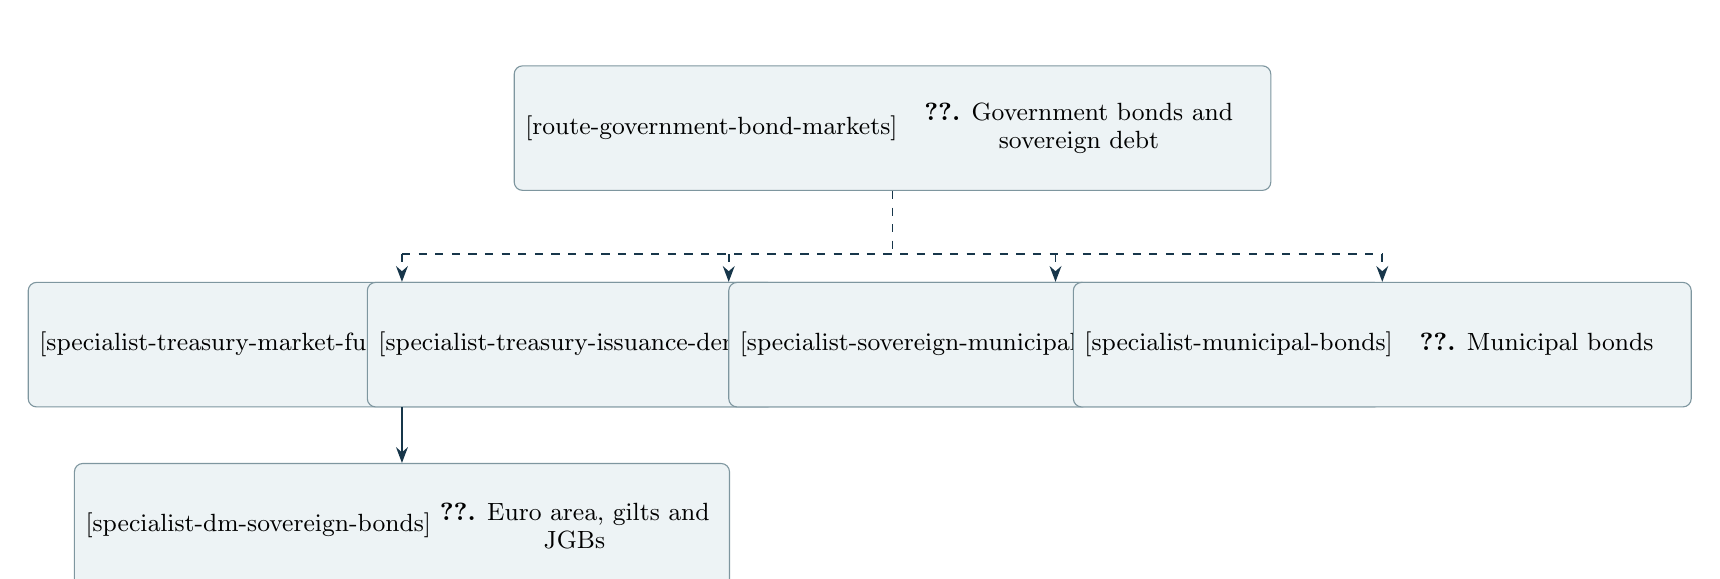
\begin{tikzpicture}[x=1cm,y=1cm]
\node[pathnode] (government-bond-markets) at (6.23,0) {\MeasurePathNode{4.6cm}{\textbf{\ref*{route-government-bond-markets}.} Government bonds and sovereign debt}\hyperref[route-government-bond-markets]{\parbox[c][\pathnodeheight][c]{4.6cm}{\centering \textbf{\ref*{route-government-bond-markets}.} Government bonds and sovereign debt}}};
\node[pathnode] (treasury-market-functioning) at (0.00,-2.75) {\MeasurePathNode{3.65cm}{\textbf{\ref*{specialist-treasury-market-functioning}.} Treasury market functioning}\hyperref[specialist-treasury-market-functioning]{\parbox[c][\pathnodeheight][c]{3.65cm}{\centering \textbf{\ref*{specialist-treasury-market-functioning}.} Treasury market functioning}}};
\node[pathnode] (treasury-issuance-demand) at (4.15,-2.75) {\MeasurePathNode{3.65cm}{\textbf{\ref*{specialist-treasury-issuance-demand}.} Issuance, auctions and demand}\hyperref[specialist-treasury-issuance-demand]{\parbox[c][\pathnodeheight][c]{3.65cm}{\centering \textbf{\ref*{specialist-treasury-issuance-demand}.} Issuance, auctions and demand}}};
\node[pathnode] (sovereign-municipal) at (8.30,-2.75) {\MeasurePathNode{3.65cm}{\textbf{\ref*{specialist-sovereign-municipal}.} Sovereign default and restructuring}\hyperref[specialist-sovereign-municipal]{\parbox[c][\pathnodeheight][c]{3.65cm}{\centering \textbf{\ref*{specialist-sovereign-municipal}.} Sovereign default and restructuring}}};
\node[pathnode] (municipal-bonds) at (12.45,-2.75) {\MeasurePathNode{3.65cm}{\textbf{\ref*{specialist-municipal-bonds}.} Municipal bonds}\hyperref[specialist-municipal-bonds]{\parbox[c][\pathnodeheight][c]{3.65cm}{\centering \textbf{\ref*{specialist-municipal-bonds}.} Municipal bonds}}};
\node[pathnode] (dm-sovereign-bonds) at (0.00,-5.05) {\MeasurePathNode{3.65cm}{\textbf{\ref*{specialist-dm-sovereign-bonds}.} Euro area, gilts and JGBs}\hyperref[specialist-dm-sovereign-bonds]{\parbox[c][\pathnodeheight][c]{3.65cm}{\centering \textbf{\ref*{specialist-dm-sovereign-bonds}.} Euro area, gilts and JGBs}}};
\draw[entryline] (government-bond-markets.south) -- (6.23,-1.60);
\draw[entryline] (0.00,-1.60) -- (12.45,-1.60);
\draw[entryarrow] (0.00,-1.60) -- (treasury-market-functioning.north);
\draw[entryarrow] (4.15,-1.60) -- (treasury-issuance-demand.north);
\draw[entryarrow] (8.30,-1.60) -- (sovereign-municipal.north);
\draw[entryarrow] (12.45,-1.60) -- (municipal-bonds.north);
\draw[patharrow] (treasury-market-functioning.south) -- (dm-sovereign-bonds.north);
\end{tikzpicture}\end{center}
\textbf{Overview checkpoint.} A section capstone: complete it after \hyperref[specialist-sovereign-municipal]{\ref*{specialist-sovereign-municipal}} and \hyperref[specialist-dm-sovereign-bonds]{\ref*{specialist-dm-sovereign-bonds}}.

\textbf{Bring these foundations with you.}\begin{itemize}
\item \hyperref[specialist-curve-term-structure]{Yield-curve construction and term-structure models} --- needed by \hyperref[specialist-treasury-market-functioning]{Treasury market functioning}, \hyperref[specialist-treasury-issuance-demand]{Issuance, auctions and demand}.
\item \hyperref[specialist-rates-inflation]{Inflation-linked bonds, real yields and breakevens} --- needed by \hyperref[specialist-sovereign-municipal]{Sovereign default and restructuring}.
\item \hyperref[specialist-monetary-policy-curve]{Monetary policy, balance-sheet policy and the yield curve} --- needed by \hyperref[specialist-dm-sovereign-bonds]{Euro area, gilts and JGBs}.
\end{itemize}\hyperref[learning-map]{Return to the whole-guide DAG.}
\Needspace{12\baselineskip}
\subsection{Treasury market structure, basis trades and dealer capacity}\label{specialist-treasury-market-functioning}
\textbf{Specialist pathway.} In \hyperref[route-government-bond-markets]{Government bond markets and sovereign debt}.

\textbf{Outcome.} Explain how dealer balance sheets, leverage rules, clearing and basis trades shape Treasury liquidity and stress episodes.

\textbf{Prerequisites.} Government bond markets overview; curve construction and money-market basics.

\textbf{Review first.} \hyperref[route-government-bond-markets]{Government bond markets and sovereign debt}; \hyperref[specialist-curve-term-structure]{Yield-curve construction and term-structure models}.

\textbf{Required readings, in order}
\begin{enumerate}\raggedright
\Needspace{5\baselineskip}\item \href{institutional_quantitative_finance_reading_list.pdf\#catalogue-0245}{Michael J. Fleming, Bruce Mizrach and Giang Nguyen, ``The Microstructure of a U.S. Treasury ECN: The BrokerTec Platform''}\CataloguePage{218}\NoteKey{catalogue-0245}\par \textbf{Mechanics.} Learn interdealer electronic trading on BrokerTec.
\Needspace{5\baselineskip}\item \href{institutional_quantitative_finance_reading_list.pdf\#exp-chaboud-off-run-treasury-liquidity}{Alain Chaboud, Ellen Correia Golay, Michael J. Fleming, Yesol Huh, Frank M. Keane, and Or Shachar, Liquidity and Trading Dynamics in the Off-the-Run U.S. Treasury Market}\CataloguePage{218}\NoteKey{exp-chaboud-off-run-treasury-liquidity}\par \textbf{Evidence.} Compare off-the-run liquidity with the on-the-run benchmark.
\Needspace{5\baselineskip}\item \href{institutional_quantitative_finance_reading_list.pdf\#gap-rates-treasury-futures-delivery}{CME Group, The Treasury Futures Delivery Process, Eighth Edition; CME conversion-factor detail}\CataloguePage{224}\NoteKey{gap-rates-treasury-futures-delivery}\par \textbf{Mechanics.} Account for the delivery option and cheapest-to-deliver before sizing a basis trade.
\Needspace{5\baselineskip}\item \href{institutional_quantitative_finance_reading_list.pdf\#exp-barth-kahn-treasury-basis}{Daniel Barth and R. Jay Kahn, Hedge Funds and the Treasury Cash-Futures Basis Trade}\CataloguePage{180}\NoteKey{exp-barth-kahn-treasury-basis}\par \textbf{Evidence.} Size the cash-futures basis trade.
\Needspace{5\baselineskip}\item \href{institutional_quantitative_finance_reading_list.pdf\#wide-jermann-swap-spreads}{Urban Jermann, ``Negative Swap Spreads and Limited Arbitrage''}\CataloguePage{219}\NoteKey{wide-jermann-swap-spreads}\par \textbf{Theory.} Model negative swap spreads with holding costs.
\Needspace{5\baselineskip}\item \href{institutional_quantitative_finance_reading_list.pdf\#wide-he-nagel-song}{Zhiguo He, Stefan Nagel and Zhaogang Song, ``Treasury inconvenience yields during the COVID-19 crisis''}\CataloguePage{219}\NoteKey{wide-he-nagel-song}\par \textbf{Evidence.} See Treasuries trade cheap to swaps when dealers are full.
\Needspace{5\baselineskip}\item \href{institutional_quantitative_finance_reading_list.pdf\#wide-du-hebert-li}{Wenxin Du, Benjamin Hébert and Wenhao Li, ``Intermediary balance sheets and the treasury yield curve''}\CataloguePage{219}\NoteKey{wide-du-hebert-li}\par \textbf{Evidence.} Track the shift from scarcity to balance-sheet constraint.
\Needspace{5\baselineskip}\item \href{institutional_quantitative_finance_reading_list.pdf\#wide-iawg-2021}{U.S. Treasury, Federal Reserve Board, Federal Reserve Bank of New York, SEC and CFTC staff, ``Recent Disruptions and Potential Reforms in the U.S. Treasury Market: A Staff Progress Report''}\CataloguePage{218}\NoteKey{wide-iawg-2021}\par \textbf{Evidence.} Read the official account and reform agenda.
\Needspace{5\baselineskip}\item \href{institutional_quantitative_finance_reading_list.pdf\#exp-kruttli-ltcm-redux}{Mathias S. Kruttli, Phillip J. Monin, Lubomir Petrasek, and Sumudu W. Watugala, LTCM Redux? Hedge Fund Treasury Trading, Funding Fragility, and Risk Constraints; Federal Reserve author publication record}\CataloguePage{179}\NoteKey{exp-kruttli-ltcm-redux}\par \textbf{Evidence.} Study hedge-fund funding fragility in 2020.
\Needspace{5\baselineskip}\item \href{institutional_quantitative_finance_reading_list.pdf\#exp-bis-sushko-todorov-treasury-swaps}{Vladyslav Sushko and Karamfil Todorov, Sizing Up Hedge Funds’ Relative Value Trades in US Treasuries and Interest Rate Swaps}\CataloguePage{180}\NoteKey{exp-bis-sushko-todorov-treasury-swaps}\par \textbf{Evidence.} Size swap-spread and basis trades and their April 2025 unwind.
\Needspace{5\baselineskip}\item \href{institutional_quantitative_finance_reading_list.pdf\#wide-duffie-dealer-capacity}{Darrell Duffie, Michael J. Fleming, Frank M. Keane, Claire Nelson, Or Shachar and Peter Van Tassel, ``Dealer Capacity and US Treasury Market Functionality''}\CataloguePage{180}\NoteKey{wide-duffie-dealer-capacity}\par \textbf{Evidence.} Measure dealer utilisation and functionality.
\Needspace{5\baselineskip}\item \href{institutional_quantitative_finance_reading_list.pdf\#w3-brauning-stein-dealer}{Falk Bräuning and Hillary Stein, ``The Effect of Primary Dealer Constraints on Intermediation in the Treasury Market''}\CataloguePage{220}\NoteKey{w3-brauning-stein-dealer}\par \textbf{Evidence.} Trace SLR and desk-VaR shocks to Treasury liquidity.
\Needspace{5\baselineskip}\item \href{institutional_quantitative_finance_reading_list.pdf\#wide-liang-zhu-clearing}{Nellie Liang and Haoxiang Zhu, ``Clearing the Path for Treasury Market Resilience''}\CataloguePage{180}\NoteKey{wide-liang-zhu-clearing}\par \textbf{Implementation.} Estimate netting benefits from cleared repo and SLR design.
\Needspace{5\baselineskip}\item \href{institutional_quantitative_finance_reading_list.pdf\#exp-treasury-clearing}{US Securities and Exchange Commission, Treasury Clearing Implementation}\CataloguePage{539}\NoteKey{exp-treasury-clearing}\par \textbf{Regulation.} Track the SEC clearing mandate timeline.
\Needspace{5\baselineskip}\item \href{institutional_quantitative_finance_reading_list.pdf\#rt-eslr-final-rule-2025}{Board of Governors of the Federal Reserve System, Federal Deposit Insurance Corporation and Office of the Comptroller of the Currency, Enhanced Supplementary Leverage Ratio Standards: Final Rule; Federal Register notice}\CataloguePage{220}\NoteKey{rt-eslr-final-rule-2025}\par \textbf{Regulation.} Recompute leverage capacity under the eSLR buffer effective 1 April 2026.
\end{enumerate}
\Needspace{5\baselineskip}\textbf{Checkpoint.} Using public data (primary-dealer positions, swap spreads, futures basis, auction results and aggregate hedge-fund positions), document March 2020 and April 2025. Show the dealer-capacity mechanism, separate cash--futures basis from swap-spread positions, and recompute the balance-sheet arithmetic under central clearing and the eSLR buffer that took effect on 1 April 2026.

\textbf{Optional branches.} \href{institutional_quantitative_finance_reading_list.pdf\#wide-fll-tips-puzzle}{Study a persistent TIPS--Treasury mispricing.}\BranchPage{228} \href{institutional_quantitative_finance_reading_list.pdf\#w3-li-petrasek-tian-dealer-var}{See desk risk limits bind in stress.}\BranchPage{219} \href{institutional_quantitative_finance_reading_list.pdf\#w3-acharya-laarits-convenience}{Relate convenience yields to hedging value.}\BranchPage{219} \href{institutional_quantitative_finance_reading_list.pdf\#w3-diamond-vantassel-convenience}{Compare convenience yields across currencies.}\BranchPage{219} \href{institutional_quantitative_finance_reading_list.pdf\#w3-eisenbach-phelan-safe-fragility}{Model March 2020 safe-asset fragility.}\BranchPage{219} \href{institutional_quantitative_finance_reading_list.pdf\#w5-schrimpf-shin-sushko}{Trace margin spirals in March 2020.}\BranchPage{180} \href{institutional_quantitative_finance_reading_list.pdf\#w5-vissing-jorgensen-2020}{Decompose spring-2020 Treasury selling.}\BranchPage{180} \href{institutional_quantitative_finance_reading_list.pdf\#rt-fleming-remolona-1999}{See how prices and liquidity absorb macro announcements.}\BranchPage{220} \href{institutional_quantitative_finance_reading_list.pdf\#rt-brandt-kavajecz-2004}{Link order flow to yield-curve moves.}\BranchPage{220} \href{institutional_quantitative_finance_reading_list.pdf\#exp-monin-treasury-decomposition}{Decompose hedge funds' Treasury exposures by strategy.}\BranchPage{180} \href{institutional_quantitative_finance_reading_list.pdf\#wide-burghardt-basis}{Work through Treasury futures basis mechanics.}\BranchPage{213}
\par{\small \hyperref[learning-map]{Learning pathway DAG} \textbar{} \hyperref[route-government-bond-markets]{Section overview} \textbar{} \hyperref[map-government-bond-markets]{Section DAG}\NoteKey{treasury-market-functioning}}
\Needspace{12\baselineskip}
\subsection{Government debt issuance, auctions and investor demand}\label{specialist-treasury-issuance-demand}
\textbf{Specialist pathway.} In \hyperref[route-government-bond-markets]{Government bond markets and sovereign debt}.

\textbf{Outcome.} Explain how auction design, the issuance calendar, debt maturity choice and investor demand set the supply and price of government debt.

\textbf{Prerequisites.} Government bond markets overview; curve construction; auction and demand-system basics.

\textbf{Review first.} \hyperref[route-government-bond-markets]{Government bond markets and sovereign debt}; \hyperref[specialist-curve-term-structure]{Yield-curve construction and term-structure models}.

\textbf{Required readings, in order}
\begin{enumerate}\raggedright
\Needspace{5\baselineskip}\item \href{institutional_quantitative_finance_reading_list.pdf\#rt-garbade-rpi-2015}{Kenneth D. Garbade, \emph{Treasury Debt Management under the Rubric of Regular and Predictable Issuance: 1983--2012}}\CataloguePage{222}\NoteKey{rt-garbade-rpi-2015}\par \textbf{Mechanics.} Learn how regular and predictable issuance adapts to financing needs.
\Needspace{5\baselineskip}\item \href{institutional_quantitative_finance_reading_list.pdf\#rt-treasury-quarterly-refunding}{U.S. Department of the Treasury, Quarterly Refunding}\CataloguePage{222}\NoteKey{rt-treasury-quarterly-refunding}\par \textbf{Data.} Read refunding statements and advisory-committee materials at their dates.
\Needspace{5\baselineskip}\item \href{institutional_quantitative_finance_reading_list.pdf\#gapclose-treasury-auction-data}{U.S. Department of the Treasury, TreasuryDirect, Historical Auction Search and About Auctions}\CataloguePage{227}\NoteKey{gapclose-treasury-auction-data}\par \textbf{Data.} Retrieve CUSIP-level auction results and allotments.
\Needspace{5\baselineskip}\item \href{institutional_quantitative_finance_reading_list.pdf\#rt-hkz-auctions-2018}{Ali Hortaçsu, Jakub Kastl and Allen Zhang, ``Bid Shading and Bidder Surplus in the US Treasury Auction System''}\CataloguePage{223}\NoteKey{rt-hkz-auctions-2018}\par \textbf{Evidence.} Estimate bid shading and dealer surplus in Treasury auctions.
\Needspace{5\baselineskip}\item \href{institutional_quantitative_finance_reading_list.pdf\#rt-lyz-auctions-2013}{Dong Lou, Hongjun Yan and Jinfan Zhang, ``Anticipated and Repeated Shocks in Liquid Markets''}\CataloguePage{223}\NoteKey{rt-lyz-auctions-2013}\par \textbf{Evidence.} Measure predictable price pressure around auctions.
\Needspace{5\baselineskip}\item \href{institutional_quantitative_finance_reading_list.pdf\#latest-fleming-auction-price-pressure-2026}{Michael J. Fleming, Weiling Liu and Giang Nguyen, Intraday Price Pressure and Order Flow Around U.S. Treasury Auctions}\CataloguePage{218}\NoteKey{latest-fleming-auction-price-pressure-2026}\par \textbf{Evidence.} Trace intraday auction pressure to dealer capacity.
\Needspace{5\baselineskip}\item \href{institutional_quantitative_finance_reading_list.pdf\#w3-lou-pinter-yield-drifts}{Dong Lou, Gabor Pinter, Semih Üslü and Danny Walker, ``Yield drifts when issuance comes before macro news''}\CataloguePage{219}\NoteKey{w3-lou-pinter-yield-drifts}\par \textbf{Evidence.} See yields drift when issuance precedes macro news.
\Needspace{5\baselineskip}\item \href{institutional_quantitative_finance_reading_list.pdf\#rt-greenwood-vayanos-2014}{Robin Greenwood and Dimitri Vayanos, ``Bond Supply and Excess Bond Returns''}\CataloguePage{223}\NoteKey{rt-greenwood-vayanos-2014}\par \textbf{Evidence.} Relate the maturity of debt supply to term premia.
\Needspace{5\baselineskip}\item \href{institutional_quantitative_finance_reading_list.pdf\#rt-ghs-maturity-2015}{Robin Greenwood, Samuel G. Hanson and Jeremy C. Stein, ``A Comparative-Advantage Approach to Government Debt Maturity''}\CataloguePage{223}\NoteKey{rt-ghs-maturity-2015}\par \textbf{Theory.} Weigh the government's maturity choice against private money-like debt.
\Needspace{5\baselineskip}\item \href{institutional_quantitative_finance_reading_list.pdf\#wide-krishnamurthy-vj}{Arvind Krishnamurthy and Annette Vissing-Jorgensen, ``The Aggregate Demand for Treasury Debt''}\CataloguePage{215}\NoteKey{wide-krishnamurthy-vj}\par \textbf{Evidence.} Measure the convenience demand for Treasuries.
\Needspace{5\baselineskip}\item \href{institutional_quantitative_finance_reading_list.pdf\#rt-jlvx-debt-puzzle-2024}{Zhengyang Jiang, Hanno Lustig, Stijn Van Nieuwerburgh and Mindy Z. Xiaolan, ``The U.S. Public Debt Valuation Puzzle''}\CataloguePage{223}\NoteKey{rt-jlvx-debt-puzzle-2024}\par \textbf{Theory.} Compare debt value with the risky present value of surpluses.
\Needspace{5\baselineskip}\item \href{institutional_quantitative_finance_reading_list.pdf\#rt-ray-droste-gorodnichenko-2024}{Walker Ray, Michael Droste and Yuriy Gorodnichenko, ``Unbundling Quantitative Easing: Taking a Cue from Treasury Auctions''}\CataloguePage{223}\NoteKey{rt-ray-droste-gorodnichenko-2024}\par \textbf{Evidence.} Use auction surprises to identify preferred-habitat demand.
\Needspace{5\baselineskip}\item \href{institutional_quantitative_finance_reading_list.pdf\#w3-boneva-qe-auctions}{Lena Boneva, Jakub Kastl and Filip Zikes, ``Dealer balance sheets and bidding behavior in the Bank of England’s QE reverse auctions''}\CataloguePage{219}\NoteKey{w3-boneva-qe-auctions}\par \textbf{Evidence.} Study dealer balance sheets in a central bank's reverse auctions.
\Needspace{5\baselineskip}\item \href{institutional_quantitative_finance_reading_list.pdf\#rt-ahmed-aldasoro-stablecoins}{Rashad Ahmed and Iñaki Aldasoro, Stablecoins and safe asset prices}\CataloguePage{223}\NoteKey{rt-ahmed-aldasoro-stablecoins}\par \textbf{Evidence.} Assess stablecoin reserve demand for Treasury bills.
\end{enumerate}
\Needspace{5\baselineskip}\textbf{Checkpoint.} Choose one quarterly refunding. From the dated statement and auction results, compute each auction's bid-to-cover ratio and allotment shares by bidder class, and measure secondary-market yield changes in the days around each auction. Relate them to the announced change in coupon sizes and bill share, a convenience-yield measure and primary-dealer positions. State which effects require when-issued or intraday data you do not have.

\textbf{Optional branches.} \href{institutional_quantitative_finance_reading_list.pdf\#exp-cordes-infante-repo-issuance-qt}{Trace Treasury issuance into repo rates.}\BranchPage{177} \href{institutional_quantitative_finance_reading_list.pdf\#w3-he-song-agency-mbs}{Compare agency MBS as a safe asset.}\BranchPage{258} \href{institutional_quantitative_finance_reading_list.pdf\#w3-diamond-vantassel-convenience}{Compare convenience yields across currencies.}\BranchPage{219}
\par{\small \hyperref[learning-map]{Learning pathway DAG} \textbar{} \hyperref[route-government-bond-markets]{Section overview} \textbar{} \hyperref[map-government-bond-markets]{Section DAG}\NoteKey{treasury-issuance-demand}}
\Needspace{12\baselineskip}
\subsection{Sovereign default, restructuring and local-currency debt}\label{specialist-sovereign-municipal}
\textbf{Specialist pathway.} In \hyperref[route-government-bond-markets]{Government bond markets and sovereign debt}.

\textbf{Outcome.} Distinguish local-currency sovereign risk, default incentives, restructuring terms and litigation risk, and compare market-implied recovery with historical outcomes.

\textbf{Prerequisites.} Government bond markets overview; inflation-linked and real yields; credit spreads and fiscal-accounting basics.

\textbf{Review first.} \hyperref[route-government-bond-markets]{Government bond markets and sovereign debt}; \hyperref[specialist-rates-inflation]{Inflation-linked bonds, real yields and breakevens}.

\textbf{Required readings, in order}
\begin{enumerate}\raggedright
\Needspace{5\baselineskip}\item \href{institutional_quantitative_finance_reading_list.pdf\#gap-sovereign-local-currency}{Wenxin Du and Jesse Schreger, Local Currency Sovereign Risk}\CataloguePage{229}\NoteKey{gap-sovereign-local-currency}\par \textbf{Mechanics.} Separate currency, inflation and default exposure in local debt.
\Needspace{5\baselineskip}\item \href{institutional_quantitative_finance_reading_list.pdf\#rt-arellano-2008}{Cristina Arellano, ``Default Risk and Income Fluctuations in Emerging Economies''}\CataloguePage{231}\NoteKey{rt-arellano-2008}\par \textbf{Theory.} Model default incentives and spreads over the cycle.
\Needspace{5\baselineskip}\item \href{institutional_quantitative_finance_reading_list.pdf\#rt-dps-portfolios-2020}{Wenxin Du, Carolin E. Pflueger and Jesse Schreger, ``Sovereign Debt Portfolios, Bond Risks, and the Credibility of Monetary Policy''}\CataloguePage{231}\NoteKey{rt-dps-portfolios-2020}\par \textbf{Evidence.} Link currency composition to monetary credibility.
\Needspace{5\baselineskip}\item \href{institutional_quantitative_finance_reading_list.pdf\#rt-hss-em-premia-2020}{Boris Hofmann, Ilhyock Shim and Hyun Song Shin, ``Bond Risk Premia and The Exchange Rate''}\CataloguePage{231}\NoteKey{rt-hss-em-premia-2020}\par \textbf{Evidence.} Relate local-bond premia to the dollar exchange rate.
\Needspace{5\baselineskip}\item \href{institutional_quantitative_finance_reading_list.pdf\#gap-sovereign-restructuring-playbook}{Global Sovereign Debt Roundtable co-chairs, Sovereign Debt Restructuring: A Playbook for Country Authorities; IMF release confirming update}\CataloguePage{230}\NoteKey{gap-sovereign-restructuring-playbook}\par \textbf{Mechanics.} Trace bond terms, creditor classes and restructuring options.
\Needspace{5\baselineskip}\item \href{institutional_quantitative_finance_reading_list.pdf\#gap-sovereign-imf-srdsf}{International Monetary Fund, Staff Guidance Note on the Sovereign Risk and Debt Sustainability Framework for Market Access Countries; IMF framework and template hub}\CataloguePage{230}\NoteKey{gap-sovereign-imf-srdsf}\par \textbf{Valuation.} Frame debt sustainability and scenario-based payment capacity.
\Needspace{5\baselineskip}\item \href{institutional_quantitative_finance_reading_list.pdf\#gap-sovereign-haircuts}{Juan J. Cruces and Christoph Trebesch, Sovereign Defaults: The Price of Haircuts}\CataloguePage{230}\NoteKey{gap-sovereign-haircuts}\par \textbf{Evidence.} Compare past restructuring outcomes with contractual recovery assumptions.
\Needspace{5\baselineskip}\item \href{institutional_quantitative_finance_reading_list.pdf\#rt-hebert-schreger-2017}{Benjamin Hébert and Jesse Schreger, ``The Costs of Sovereign Default: Evidence from Argentina''}\CataloguePage{231}\NoteKey{rt-hebert-schreger-2017}\par \textbf{Evidence.} Estimate the cost of default from legal rulings.
\Needspace{5\baselineskip}\item \href{institutional_quantitative_finance_reading_list.pdf\#rt-ste-court-2021}{Julian Schumacher, Christoph Trebesch and Henrik Enderlein, ``Sovereign defaults in court''}\CataloguePage{231}\NoteKey{rt-ste-court-2021}\par \textbf{Evidence.} Track creditor litigation and holdout risk.
\Needspace{5\baselineskip}\item \href{institutional_quantitative_finance_reading_list.pdf\#gap-sovereign-worldbank-ids}{World Bank, International Debt Statistics; World Bank access and archive guidance}\CataloguePage{230}\NoteKey{gap-sovereign-worldbank-ids}\par \textbf{Data.} Use dated external-debt series with coverage and revision checks.
\Needspace{5\baselineskip}\item \href{institutional_quantitative_finance_reading_list.pdf\#latest-avdjiev-sovereign-nbfi-nexus-2026}{Stefan Avdjiev, Bryan Hardy and Maximilian Jager, The Evolving Nexus: Sovereigns, Banks and NBFIs}\CataloguePage{230}\NoteKey{latest-avdjiev-sovereign-nbfi-nexus-2026}\par \textbf{Evidence.} Extend sovereign--bank exposure analysis to nonbank investors and their bank financing.
\end{enumerate}
\Needspace{5\baselineskip}\textbf{Checkpoint.} For one sovereign restructuring, draw the contractual cash-flow tree of the old and new bonds, identify the dated disclosure and debt-sustainability set, and compare market-implied recovery with historical haircuts and the IMF scenarios. Separate currency, inflation and default exposure in the same issuer's local-currency bonds. State where licensed quotes or full bond documents are unavailable, and map one sovereign--bank--nonbank exposure chain without treating co-movement as realised contagion.

\textbf{Optional branches.} \href{institutional_quantitative_finance_reading_list.pdf\#wide-lpps-sovereign}{See global drivers of sovereign CDS.}\BranchPage{230} \href{institutional_quantitative_finance_reading_list.pdf\#wide-pan-singleton-sovereign}{Infer default and recovery from the sovereign CDS term structure.}\BranchPage{230}
\par{\small \hyperref[learning-map]{Learning pathway DAG} \textbar{} \hyperref[route-government-bond-markets]{Section overview} \textbar{} \hyperref[map-government-bond-markets]{Section DAG}\NoteKey{sovereign-municipal}}
\Needspace{12\baselineskip}
\subsection{Municipal bonds: pledges, taxes, trading costs and climate risk}\label{specialist-municipal-bonds}
\textbf{Specialist pathway.} In \hyperref[route-government-bond-markets]{Government bond markets and sovereign debt}.

\textbf{Outcome.} Value a municipal bond from its security pledge, tax treatment, disclosure record and trading costs, and separate default, liquidity, tax and climate risk in its spread.

\textbf{Prerequisites.} Government bond markets overview; tax-equivalent yield and credit-spread basics.

\textbf{Review first.} \hyperref[route-government-bond-markets]{Government bond markets and sovereign debt}.

\textbf{Required readings, in order}
\begin{enumerate}\raggedright
\Needspace{5\baselineskip}\item \href{institutional_quantitative_finance_reading_list.pdf\#gap-muni-repayment-pledges}{Municipal Securities Rulemaking Board, Sources of Repayment; MSRB guide to bond-specific federal and state tax treatment}\CataloguePage{233}\NoteKey{gap-muni-repayment-pledges}\par \textbf{Mechanics.} Identify security and revenue pledges before valuing a municipal claim.
\Needspace{5\baselineskip}\item \href{institutional_quantitative_finance_reading_list.pdf\#gap-muni-emma}{Municipal Securities Rulemaking Board, EMMA: Electronic Municipal Market Access; MSRB coverage and caveats}\CataloguePage{233}\NoteKey{gap-muni-emma}\par \textbf{Data.} Retrieve trade and continuing-disclosure records at the decision date.
\Needspace{5\baselineskip}\item \href{institutional_quantitative_finance_reading_list.pdf\#gap-muni-trading-costs}{Lawrence E. Harris and Michael S. Piwowar, Secondary Trading Costs in the Municipal Bond Market}\CataloguePage{233}\NoteKey{gap-muni-trading-costs}\par \textbf{Implementation.} Apply market-specific size and customer-trade cost evidence.
\Needspace{5\baselineskip}\item \href{institutional_quantitative_finance_reading_list.pdf\#rt-ghs-muni-2007}{Richard C. Green, Burton Hollifield and Norman Schürhoff, ``Financial Intermediation and the Costs of Trading in an Opaque Market''}\CataloguePage{234}\NoteKey{rt-ghs-muni-2007}\par \textbf{Evidence.} Measure dealer markups and market power in an opaque market.
\Needspace{5\baselineskip}\item \href{institutional_quantitative_finance_reading_list.pdf\#wide-ang-bhansali-xing}{Andrew Ang, Vineer Bhansali and Yuhang Xing, ``Taxes on Tax-Exempt Bonds''}\CataloguePage{234}\NoteKey{wide-ang-bhansali-xing}\par \textbf{Evidence.} Price the tax treatment of tax-exempt bonds.
\Needspace{5\baselineskip}\item \href{institutional_quantitative_finance_reading_list.pdf\#wide-schwert-muni}{Michael Schwert, ``Municipal Bond Liquidity and Default Risk''}\CataloguePage{233}\NoteKey{wide-schwert-muni}\par \textbf{Evidence.} Separate default and liquidity in municipal spreads.
\Needspace{5\baselineskip}\item \href{institutional_quantitative_finance_reading_list.pdf\#gap-muni-pension-fiscal-spreads}{Robert Novy-Marx and Joshua D. Rauh, Fiscal Imbalances and Borrowing Costs: Evidence from State Investment Losses}\CataloguePage{233}\NoteKey{gap-muni-pension-fiscal-spreads}\par \textbf{Evidence.} Study how fiscal obligations can enter municipal spreads.
\Needspace{5\baselineskip}\item \href{institutional_quantitative_finance_reading_list.pdf\#rt-painter-2020}{Marcus Painter, ``An inconvenient cost: The effects of climate change on municipal bonds''}\CataloguePage{234}\NoteKey{rt-painter-2020}\par \textbf{Evidence.} Test whether climate exposure raises long-term issuance costs.
\Needspace{5\baselineskip}\item \href{institutional_quantitative_finance_reading_list.pdf\#rt-ggls-sealevel-2023}{Paul Goldsmith-Pinkham, Matthew T. Gustafson, Ryan C. Lewis and Michael Schwert, ``Sea-Level Rise Exposure and Municipal Bond Yields''}\CataloguePage{234}\NoteKey{rt-ggls-sealevel-2023}\par \textbf{Evidence.} Price sea-level-rise exposure with a structural credit model.
\end{enumerate}
\Needspace{5\baselineskip}\textbf{Checkpoint.} For one revenue bond and one general-obligation bond, identify the pledge and tax treatment, retrieve EMMA trades and continuing disclosures at the decision date, compute tax-adjusted spreads to Treasuries, estimate round-trip costs by trade size, and attribute each spread to default, liquidity, tax and climate exposure. State where full official statements or licensed data are missing.

\par{\small \hyperref[learning-map]{Learning pathway DAG} \textbar{} \hyperref[route-government-bond-markets]{Section overview} \textbar{} \hyperref[map-government-bond-markets]{Section DAG}\NoteKey{municipal-bonds}}
\Needspace{12\baselineskip}
\subsection{Euro-area, UK and Japanese government bond markets}\label{specialist-dm-sovereign-bonds}
\textbf{Specialist pathway.} In \hyperref[route-government-bond-markets]{Government bond markets and sovereign debt}.

\textbf{Outcome.} Explain euro-area spread fragmentation, central-bank backstops, the 2022 gilt crisis and the reduction of JGB purchases, and judge what each implies for spread and liquidity risk.

\textbf{Prerequisites.} Treasury market structure; monetary and balance-sheet policy; sovereign spread basics.

\textbf{Review first.} \hyperref[specialist-treasury-market-functioning]{Treasury market structure, basis trades and dealer capacity}; \hyperref[specialist-monetary-policy-curve]{Monetary policy, balance-sheet policy and the yield curve}.

\textbf{Required readings, in order}
\begin{enumerate}\raggedright
\Needspace{5\baselineskip}\item \href{institutional_quantitative_finance_reading_list.pdf\#rt-bbk-flight-2009}{Alessandro Beber, Michael W. Brandt and Kenneth A. Kavajecz, ``Flight-to-Quality or Flight-to-Liquidity? Evidence from the Euro-Area Bond Market''}\CataloguePage{232}\NoteKey{rt-bbk-flight-2009}\par \textbf{Evidence.} Separate credit quality from liquidity in euro-area spreads.
\Needspace{5\baselineskip}\item \href{institutional_quantitative_finance_reading_list.pdf\#rt-degrauwe-ji-2013}{Paul De Grauwe and Yuemei Ji, ``Self-fulfilling crises in the Eurozone: An empirical test''}\CataloguePage{232}\NoteKey{rt-degrauwe-ji-2013}\par \textbf{Evidence.} Test for self-fulfilling spread dynamics in the euro crisis.
\Needspace{5\baselineskip}\item \href{institutional_quantitative_finance_reading_list.pdf\#rt-ads-pyrrhic-2014}{Viral Acharya, Itamar Drechsler and Philipp Schnabl, ``A Pyrrhic Victory? Bank Bailouts and Sovereign Credit Risk''}\CataloguePage{232}\NoteKey{rt-ads-pyrrhic-2014}\par \textbf{Evidence.} Trace the sovereign--bank loop from bailouts to CDS.
\Needspace{5\baselineskip}\item \href{institutional_quantitative_finance_reading_list.pdf\#rt-pstu-2016}{Loriana Pelizzon, Marti G. Subrahmanyam, Davide Tomio and Jun Uno, ``Sovereign credit risk, liquidity, and European Central Bank intervention: Deus ex machina?''}\CataloguePage{232}\NoteKey{rt-pstu-2016}\par \textbf{Evidence.} Link credit risk, market-maker liquidity and ECB operations.
\Needspace{5\baselineskip}\item \href{institutional_quantitative_finance_reading_list.pdf\#rt-knvj-ecb-2018}{Arvind Krishnamurthy, Stefan Nagel and Annette Vissing-Jorgensen, ``ECB Policies Involving Government Bond Purchases: Impact and Channels''}\CataloguePage{232}\NoteKey{rt-knvj-ecb-2018}\par \textbf{Evidence.} Decompose the yield effects of the SMP and OMT.
\Needspace{5\baselineskip}\item \href{institutional_quantitative_finance_reading_list.pdf\#rt-koijen-euro-qe-2021}{Ralph S. J. Koijen, François Koulischer, Benoît Nguyen and Motohiro Yogo, ``Inspecting the mechanism of quantitative easing in the euro area''}\CataloguePage{232}\NoteKey{rt-koijen-euro-qe-2021}\par \textbf{Evidence.} Identify who sold to the Eurosystem under QE.
\Needspace{5\baselineskip}\item \href{institutional_quantitative_finance_reading_list.pdf\#rt-ecb-tpi-2022}{European Central Bank, The Transmission Protection Instrument}\CataloguePage{232}\NoteKey{rt-ecb-tpi-2022}\par \textbf{Regulation.} Read the TPI's eligibility criteria and limits.
\Needspace{5\baselineskip}\item \href{institutional_quantitative_finance_reading_list.pdf\#rt-pinter-gilt-2023}{Gabor Pinter, An anatomy of the 2022 gilt market crisis}\CataloguePage{233}\NoteKey{rt-pinter-gilt-2023}\par \textbf{Evidence.} Dissect the 2022 gilt and LDI crisis with transaction data.
\Needspace{5\baselineskip}\item \href{institutional_quantitative_finance_reading_list.pdf\#depth-alm-bis-firesales-2024}{Gabor Pinter, Emil Siriwardane and Danny Walker, Fire Sales of Safe Assets}\CataloguePage{114}\NoteKey{depth-alm-bis-firesales-2024}\par \textbf{Evidence.} Measure price impact from fire sales of safe assets.
\Needspace{5\baselineskip}\item \href{institutional_quantitative_finance_reading_list.pdf\#gap-gilt-resilience}{Sarah Breeden, Bank of England, Gilt edged resilience: strengthening liquidity provision in the repo market; September 2025 discussion paper}\CataloguePage{177}\NoteKey{gap-gilt-resilience}\par \textbf{Regulation.} Assess proposed gilt-repo resilience reforms.
\Needspace{5\baselineskip}\item \href{institutional_quantitative_finance_reading_list.pdf\#gap-jgb-qqe}{Noritaka Fukuma, Tomiyuki Kitamura, Kohei Maehashi, Naoki Matsuda, Keita Takemura and Kota Watanabe, The Impact of Quantitative and Qualitative Easing and Yield Curve Control on the Functioning of the Japanese Government Bond Market}\CataloguePage{310}\NoteKey{gap-jgb-qqe}\par \textbf{Evidence.} Measure how QQE and yield-curve control changed JGB market functioning.
\Needspace{5\baselineskip}\item \href{institutional_quantitative_finance_reading_list.pdf\#gap-jgb-slf}{Joji Ide, Tomoaki Masuda and Masato Takahashi, Developments in the Functioning of the JGB Markets from the Perspective of the Usage of the Securities Lending Facility}\CataloguePage{310}\NoteKey{gap-jgb-slf}\par \textbf{Evidence.} Use securities-lending facility data to track JGB scarcity.
\Needspace{5\baselineskip}\item \href{institutional_quantitative_finance_reading_list.pdf\#rt-boj-jgb-plan-2025}{Bank of Japan, Statement on Monetary Policy (June 2025), with the plan for the reduction of JGB purchases}\CataloguePage{233}\NoteKey{rt-boj-jgb-plan-2025}\par \textbf{Regulation.} Date the reduction of BoJ purchases and its review points.
\end{enumerate}
\Needspace{5\baselineskip}\textbf{Checkpoint.} Pick one episode each from the euro area (2011--12 or 2022), the United Kingdom (September--October 2022) and Japan (2022--25). For each, chart the yield or spread, a liquidity measure and the central-bank action dates; separate credit, liquidity and forced-selling effects; and state what the TPI criteria, the gilt-market reforms and the BoJ purchase plan imply for a hedged long position in the next episode.

\textbf{Optional branches.} \href{institutional_quantitative_finance_reading_list.pdf\#rt-altavilla-2019}{Use the euro-area policy-surprise database.}\BranchPage{222} \href{institutional_quantitative_finance_reading_list.pdf\#exp-gourinchas-ray-vayanos-preferred-habitat}{Model cross-border preferred-habitat spillovers.}\BranchPage{214} \href{institutional_quantitative_finance_reading_list.pdf\#w3-randl-international-bonds}{Compare international government bond portfolios.}\BranchPage{215}
\par{\small \hyperref[learning-map]{Learning pathway DAG} \textbar{} \hyperref[route-government-bond-markets]{Section overview} \textbar{} \hyperref[map-government-bond-markets]{Section DAG}\NoteKey{dm-sovereign-bonds}}
\clearpage
\section{Corporate credit, hybrids and labelled bonds}\label{route-corporate-credit-capital}
\label{route-17}
\textbf{Learning sequence.} Model default and recovery, reconcile bond spreads with CDS, then study subordinated bank and corporate hybrids and sustainability-labelled bonds.

\textbf{Section goals.} Across its pathways, this section teaches you to:
\begin{itemize}[leftmargin=1.4em,itemsep=0pt,topsep=1pt]
\item price default with structural and reduced-form models and aggregate portfolio losses (\hyperref[specialist-credit-models-default]{\ref*{specialist-credit-models-default}})
\item reconcile cash-bond spreads, CDS values and bond-return evidence (\hyperref[specialist-corporate-credit-cds]{\ref*{specialist-corporate-credit-cds}})
\item value AT1, CoCo and Tier 2 bank capital by coupon, conversion, call and resolution terms (\hyperref[specialist-bank-capital]{\ref*{specialist-bank-capital}})
\item value corporate hybrids and preferred shares by deferral, subordination and calls (\hyperref[specialist-corporate-hybrids-preferred]{\ref*{specialist-corporate-hybrids-preferred}})
\item separate use-of-proceeds claims, contingent coupons and pricing evidence in labelled bonds (\hyperref[specialist-sustainable-bonds]{\ref*{specialist-sustainable-bonds}})
\end{itemize}
\textbf{Overview outcome.} Decompose a bank's senior bond, CDS and AT1 or Tier 2 spreads into expected loss, liquidity and contract features, and show which claim the capital structure protects first.

\textbf{Prerequisites.} Rates: yield curves, term premia and derivatives; hazard rates, recovery, seniority and basic option exercise.

\textbf{Review first.} \hyperref[route-rates-credit-mortgages]{Rates: yield curves, term premia and derivatives}.

\textbf{Required readings, in order}
\begin{enumerate}\raggedright
\Needspace{5\baselineskip}\item \href{institutional_quantitative_finance_reading_list.pdf\#s6-duffie}{Darrell Duffie and Kenneth Singleton, \emph{Credit Risk: Pricing, Measurement, and Management}}\CataloguePage{237}\NoteKey{s6-duffie}\par Add default, recovery and credit-spread modelling without confusing spread with expected loss.
\Needspace{5\baselineskip}\item \href{institutional_quantitative_finance_reading_list.pdf\#w5-altman-mortality}{Edward I. Altman, ``Measuring Corporate Bond Mortality and Performance''}\CataloguePage{245}\NoteKey{w5-altman-mortality}\par Use cohort default and loss tables to compare a quoted spread with realised credit losses.
\Needspace{5\baselineskip}\item \href{institutional_quantitative_finance_reading_list.pdf\#exp-bao-pan-wang-bond-illiquidity}{Jack Bao, Jun Pan, and Jiang Wang, The Illiquidity of Corporate Bonds}\CataloguePage{242}\NoteKey{exp-bao-pan-wang-bond-illiquidity}\par Bring sparse trading and corporate-bond liquidity into credit valuation.
\Needspace{5\baselineskip}\item \href{institutional_quantitative_finance_reading_list.pdf\#gap-credit-distress-book}{Edward I. Altman, Edith Hotchkiss and Wei Wang, Corporate Financial Distress, Restructuring, and Bankruptcy: Analyze Leveraged Finance, Distressed Debt, and Bankruptcy, Fourth Edition}\CataloguePage{243}\NoteKey{gap-credit-distress-book}\par\emph{Selection:} Distress prediction, bankruptcy process and creditor-recovery topics (topic selection; chapter numbering is not inferred).\par Follow seniority, distress, bankruptcy and recovery across the capital structure before valuing a subordinated or hybrid claim.
\end{enumerate}
\Needspace{5\baselineskip}\textbf{Checkpoint, a section capstone: complete it after \hyperref[specialist-corporate-credit-cds]{\ref*{specialist-corporate-credit-cds}} and \hyperref[specialist-bank-capital]{\ref*{specialist-bank-capital}}.} For one bank, take a senior unsecured bond, its CDS and one AT1 or Tier 2 bond. Decompose each spread into expected loss, liquidity and contract features. Shock default probability, recovery and the coupon-cancellation or write-down trigger; explain which claim the capital structure protects first.

\par\textbf{Continue in this section.} \hyperref[specialist-credit-models-default]{Credit models, default prediction and credit portfolios}; \hyperref[specialist-corporate-credit-cds]{Corporate bonds and credit derivatives}; \hyperref[specialist-bank-capital]{Bank capital, AT1, CoCos and Tier 2}; \hyperref[specialist-corporate-hybrids-preferred]{Corporate hybrids and preferred shares}; \hyperref[specialist-sustainable-bonds]{Green, transition and sustainability-linked bonds}.
\par{\small \hyperref[learning-map]{Learning pathway DAG} \textbar{} \hyperref[map-corporate-credit-capital]{Section DAG}\NoteKey{corporate-credit-capital}}
\clearpage
\subsection*{Corporate credit, hybrids and labelled bonds: pathway DAG}\phantomsection\label{map-corporate-credit-capital}
\addcontentsline{toc}{subsection}{Corporate credit, hybrids and labelled bonds: pathway DAG}
Start with the section overview's readings, for orientation. Solid arrows show prerequisites within this section. Dashed connectors identify entry points with no further prerequisite in this section; the linked foundations below still apply. Follow the arrows for dependencies and the subsection numbers for reading order. Every node is clickable.
\begin{center}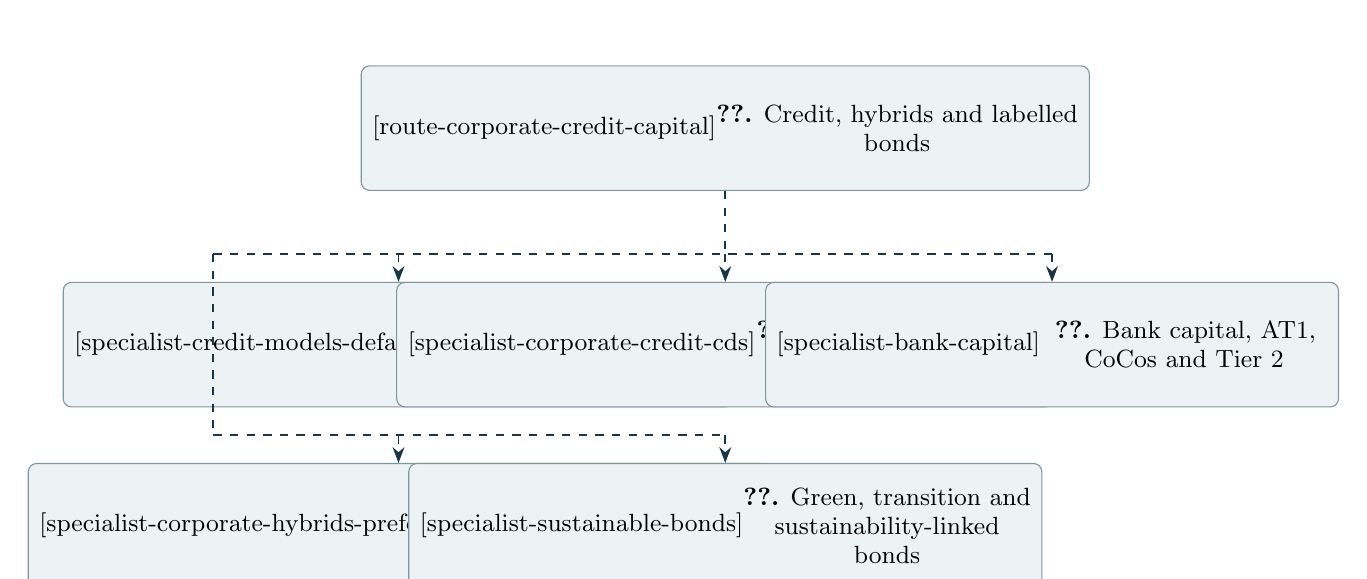
\begin{tikzpicture}[x=1cm,y=1cm]
\node[pathnode] (corporate-credit-capital) at (4.15,0) {\MeasurePathNode{4.6cm}{\textbf{\ref*{route-corporate-credit-capital}.} Credit, hybrids and labelled bonds}\hyperref[route-corporate-credit-capital]{\parbox[c][\pathnodeheight][c]{4.6cm}{\centering \textbf{\ref*{route-corporate-credit-capital}.} Credit, hybrids and labelled bonds}}};
\node[pathnode] (credit-models-default) at (0.00,-2.75) {\MeasurePathNode{3.65cm}{\textbf{\ref*{specialist-credit-models-default}.} Credit models and default}\hyperref[specialist-credit-models-default]{\parbox[c][\pathnodeheight][c]{3.65cm}{\centering \textbf{\ref*{specialist-credit-models-default}.} Credit models and default}}};
\node[pathnode] (corporate-credit-cds) at (4.15,-2.75) {\MeasurePathNode{3.65cm}{\textbf{\ref*{specialist-corporate-credit-cds}.} Corporate bonds and credit derivatives}\hyperref[specialist-corporate-credit-cds]{\parbox[c][\pathnodeheight][c]{3.65cm}{\centering \textbf{\ref*{specialist-corporate-credit-cds}.} Corporate bonds and credit derivatives}}};
\node[pathnode] (bank-capital) at (8.30,-2.75) {\MeasurePathNode{3.65cm}{\textbf{\ref*{specialist-bank-capital}.} Bank capital, AT1, CoCos and Tier 2}\hyperref[specialist-bank-capital]{\parbox[c][\pathnodeheight][c]{3.65cm}{\centering \textbf{\ref*{specialist-bank-capital}.} Bank capital, AT1, CoCos and Tier 2}}};
\node[pathnode] (corporate-hybrids-preferred) at (0.00,-5.05) {\MeasurePathNode{3.65cm}{\textbf{\ref*{specialist-corporate-hybrids-preferred}.} Corporate hybrids and preferred shares}\hyperref[specialist-corporate-hybrids-preferred]{\parbox[c][\pathnodeheight][c]{3.65cm}{\centering \textbf{\ref*{specialist-corporate-hybrids-preferred}.} Corporate hybrids and preferred shares}}};
\node[pathnode] (sustainable-bonds) at (4.15,-5.05) {\MeasurePathNode{3.65cm}{\textbf{\ref*{specialist-sustainable-bonds}.} Green, transition and sustainability-linked bonds}\hyperref[specialist-sustainable-bonds]{\parbox[c][\pathnodeheight][c]{3.65cm}{\centering \textbf{\ref*{specialist-sustainable-bonds}.} Green, transition and sustainability-linked bonds}}};
\draw[entryline] (corporate-credit-capital.south) -- (4.15,-1.60);
\draw[entryline] (-2.35,-1.60) -- (-2.35,-3.90);
\draw[entryline] (-2.35,-1.60) -- (8.30,-1.60);
\draw[entryarrow] (0.00,-1.60) -- (credit-models-default.north);
\draw[entryarrow] (4.15,-1.60) -- (corporate-credit-cds.north);
\draw[entryarrow] (8.30,-1.60) -- (bank-capital.north);
\draw[entryline] (-2.35,-3.90) -- (4.15,-3.90);
\draw[entryarrow] (0.00,-3.90) -- (corporate-hybrids-preferred.north);
\draw[entryarrow] (4.15,-3.90) -- (sustainable-bonds.north);
\end{tikzpicture}\end{center}
\textbf{Overview checkpoint.} A section capstone: complete it after \hyperref[specialist-corporate-credit-cds]{\ref*{specialist-corporate-credit-cds}} and \hyperref[specialist-bank-capital]{\ref*{specialist-bank-capital}}.

\textbf{Bring these foundations with you.}\begin{itemize}
\item \hyperref[specialist-rates-inflation]{Inflation-linked bonds, real yields and breakevens} --- needed by \hyperref[specialist-corporate-credit-cds]{Corporate bonds and credit derivatives}.
\end{itemize}\hyperref[learning-map]{Return to the whole-guide DAG.}
\Needspace{12\baselineskip}
\subsection{Credit models, default prediction and credit portfolios}\label{specialist-credit-models-default}
\textbf{Specialist pathway.} In \hyperref[route-corporate-credit-capital]{Corporate credit, hybrids and labelled bonds}.

\textbf{Outcome.} Price credit risk with structural and reduced-form models, estimate default probabilities and aggregate them into portfolio loss distributions.

\textbf{Prerequisites.} Rates overview, stochastic calculus and regression.

\textbf{Review first.} \hyperref[route-corporate-credit-capital]{Corporate credit, hybrids and labelled bonds}.

\textbf{Required readings, in order}
\begin{enumerate}\raggedright
\Needspace{5\baselineskip}\item \href{institutional_quantitative_finance_reading_list.pdf\#wide-merton-1974}{Robert C. Merton, ``On the Pricing of Corporate Debt: The Risk Structure of Interest Rates''}\CataloguePage{237}\NoteKey{wide-merton-1974}\par \textbf{Theory.} Treat equity as a call on firm assets.
\Needspace{5\baselineskip}\item \href{institutional_quantitative_finance_reading_list.pdf\#wide-black-cox}{Fischer Black and John C. Cox, ``Valuing Corporate Securities: Some Effects of Bond Indenture Provisions''}\CataloguePage{237}\NoteKey{wide-black-cox}\par \textbf{Theory.} Add first-passage default.
\Needspace{5\baselineskip}\item \href{institutional_quantitative_finance_reading_list.pdf\#wide-leland-1994}{Hayne E. Leland, ``Corporate Debt Value, Bond Covenants, and Optimal Capital Structure''}\CataloguePage{237}\NoteKey{wide-leland-1994}\par \textbf{Theory.} Endogenise default and leverage.
\Needspace{5\baselineskip}\item \href{institutional_quantitative_finance_reading_list.pdf\#wide-jarrow-turnbull}{Robert A. Jarrow and Stuart M. Turnbull, ``Pricing Derivatives on Financial Securities Subject to Credit Risk''}\CataloguePage{238}\NoteKey{wide-jarrow-turnbull}\par \textbf{Theory.} Model default as an intensity.
\Needspace{5\baselineskip}\item \href{institutional_quantitative_finance_reading_list.pdf\#wide-duffie-singleton-1999}{Darrell Duffie and Kenneth J. Singleton, ``Modeling Term Structures of Defaultable Bonds''}\CataloguePage{238}\NoteKey{wide-duffie-singleton-1999}\par \textbf{Valuation.} Discount at default-adjusted rates.
\Needspace{5\baselineskip}\item \href{institutional_quantitative_finance_reading_list.pdf\#catalogue-0237}{David Lando, \emph{Credit Risk Modeling}}\CataloguePage{237}\NoteKey{catalogue-0237}\par \textbf{Valuation.} Consolidate credit models in a textbook.
\Needspace{5\baselineskip}\item \href{institutional_quantitative_finance_reading_list.pdf\#wide-cdgm-spread-changes}{Pierre Collin-Dufresne, Robert S. Goldstein and J. Spencer Martin, ``The Determinants of Credit Spread Changes''}\CataloguePage{238}\NoteKey{wide-cdgm-spread-changes}\par \textbf{Evidence.} See how little structural variables explain spread changes.
\Needspace{5\baselineskip}\item \href{institutional_quantitative_finance_reading_list.pdf\#wide-huang-huang-puzzle}{Jing-Zhi Huang and Ming Huang, ``How Much of the Corporate-Treasury Yield Spread Is Due to Credit Risk?''}\CataloguePage{238}\NoteKey{wide-huang-huang-puzzle}\par \textbf{Evidence.} Quantify the credit spread puzzle.
\Needspace{5\baselineskip}\item \href{institutional_quantitative_finance_reading_list.pdf\#wide-lmn-cds-basis}{Francis A. Longstaff, Sanjay Mithal and Eric Neis, ``Corporate Yield Spreads: Default Risk or Liquidity? New Evidence from the Credit Default Swap Market''}\CataloguePage{238}\NoteKey{wide-lmn-cds-basis}\par \textbf{Evidence.} Separate default and liquidity components.
\Needspace{5\baselineskip}\item \href{institutional_quantitative_finance_reading_list.pdf\#wide-shumway-hazard}{Tyler Shumway, ``Forecasting Bankruptcy More Accurately: A Simple Hazard Model''}\CataloguePage{241}\NoteKey{wide-shumway-hazard}\par \textbf{Methods.} Fit hazard-model default prediction.
\Needspace{5\baselineskip}\item \href{institutional_quantitative_finance_reading_list.pdf\#wide-chs-distress}{John Y. Campbell, Jens Hilscher and Jan Szilagyi, ``In Search of Distress Risk''}\CataloguePage{241}\NoteKey{wide-chs-distress}\par \textbf{Evidence.} Link distress to anomalous returns.
\Needspace{5\baselineskip}\item \href{institutional_quantitative_finance_reading_list.pdf\#wide-vasicek-loan}{Oldrich Vasicek, ``Loan portfolio value''}\CataloguePage{241}\NoteKey{wide-vasicek-loan}\par \textbf{Methods.} Derive the single-factor portfolio loss distribution.
\Needspace{5\baselineskip}\item \href{institutional_quantitative_finance_reading_list.pdf\#wide-gordy-asrf}{Michael B. Gordy, ``A risk-factor model foundation for ratings-based bank capital rules''}\CataloguePage{241}\NoteKey{wide-gordy-asrf}\par \textbf{Theory.} See when ratings-based capital is portfolio-invariant.
\Needspace{5\baselineskip}\item \href{institutional_quantitative_finance_reading_list.pdf\#wide-das-common-failings}{Sanjiv R. Das, Darrell Duffie, Nikunj Kapadia and Leandro Saita, ``Common Failings: How Corporate Defaults Are Correlated''}\CataloguePage{241}\NoteKey{wide-das-common-failings}\par \textbf{Counter-evidence.} Test whether defaults cluster beyond conditional models.
\end{enumerate}
\Needspace{5\baselineskip}\textbf{Checkpoint.} Estimate distance-to-default and hazard-model default probabilities for a set of issuers, map them to spreads, and build a Vasicek portfolio loss distribution; show how correlation and default clustering change the 99.9\% loss quantile.

\textbf{Optional branches.} \href{institutional_quantitative_finance_reading_list.pdf\#wide-gilchrist-zakrajsek}{Use the excess bond premium as a macro signal.}\BranchPage{238} \href{institutional_quantitative_finance_reading_list.pdf\#wide-bai-collin-dufresne-basis}{Study negative CDS-bond bases and funding.}\BranchPage{238} \href{institutional_quantitative_finance_reading_list.pdf\#wide-altman-zscore}{Compare with the historical Z-score baseline.}\BranchPage{241} \href{institutional_quantitative_finance_reading_list.pdf\#w5-altman-brady-resti-sironi}{Model the default--recovery link.}\BranchPage{245} \href{institutional_quantitative_finance_reading_list.pdf\#w5-jankowitsch-recovery}{Explain bond recovery rates.}\BranchPage{245}
\par{\small \hyperref[learning-map]{Learning pathway DAG} \textbar{} \hyperref[route-corporate-credit-capital]{Section overview} \textbar{} \hyperref[map-corporate-credit-capital]{Section DAG}\NoteKey{credit-models-default}}
\Needspace{12\baselineskip}
\subsection{Corporate bonds and credit derivatives}\label{specialist-corporate-credit-cds}
\textbf{Specialist pathway.} In \hyperref[route-corporate-credit-capital]{Corporate credit, hybrids and labelled bonds}.

\textbf{Outcome.} Reconcile a cash-bond spread, a CDS model value and competing bond-return evidence.

\textbf{Prerequisites.} Inflation-linked bonds, real yields and breakevens; hazard rates, recovery and regression.

\textbf{Review first.} \hyperref[route-corporate-credit-capital]{Corporate credit, hybrids and labelled bonds}; \hyperref[specialist-rates-inflation]{Inflation-linked bonds, real yields and breakevens}.

\textbf{Required readings, in order}
\begin{enumerate}\raggedright
\Needspace{5\baselineskip}\item \href{institutional_quantitative_finance_reading_list.pdf\#s6-duffie}{Darrell Duffie and Kenneth Singleton, \emph{Credit Risk: Pricing, Measurement, and Management}}\CataloguePage{237}\NoteKey{s6-duffie}\par \textbf{Valuation.} Define default intensity, recovery and risk-neutral credit pricing.
\Needspace{5\baselineskip}\item \href{institutional_quantitative_finance_reading_list.pdf\#catalogue-0238}{Dominic O'Kane, \emph{Modelling Single-name and Multi-name Credit Derivatives}}\CataloguePage{237}\NoteKey{catalogue-0238}\par \textbf{Mechanics.} Learn CDS coupons, upfronts, indices and tranche conventions.
\Needspace{5\baselineskip}\item \href{institutional_quantitative_finance_reading_list.pdf\#add-cds-contract}{International Swaps and Derivatives Association, 2014 Credit Derivatives Definitions; 2019 NTCE Supplement; Physical Settlement Matrix and Confirmation}\CataloguePage{239}\NoteKey{add-cds-contract}\par \textbf{Mechanics.} Map credit events and settlement to incorporated ISDA terms.
\Needspace{5\baselineskip}\item \href{institutional_quantitative_finance_reading_list.pdf\#add-cds-model}{ISDA and S\&P Global, ISDA CDS Standard Model, source code and test grids}\CataloguePage{238}\NoteKey{add-cds-model}\par \textbf{Valuation.} Reproduce a standard spread-to-upfront CDS conversion.
\Needspace{5\baselineskip}\item \href{institutional_quantitative_finance_reading_list.pdf\#add-cds-rfr2026}{ISDA and S\&P Global, RFR Interest Rate Curve Specification--6 Currencies}\CataloguePage{239}\NoteKey{add-cds-rfr2026}\par \textbf{Data.} Pin the RFR curve specification and rate inputs separately from the model version.
\Needspace{5\baselineskip}\item \href{institutional_quantitative_finance_reading_list.pdf\#add-bond-factor}{Bryan Kelly, Diogo Palhares and Seth Pruitt, Modeling Corporate Bond Returns}\CataloguePage{241}\NoteKey{add-bond-factor}\par \textbf{Evidence.} Study a conditional factor benchmark for bond returns.
\Needspace{5\baselineskip}\item \href{institutional_quantitative_finance_reading_list.pdf\#add-bond-counterevidence}{Alexander Dickerson, Philippe Mueller and Cesare Robotti, Priced Risk in Corporate Bonds; author manuscript}\CataloguePage{242}\NoteKey{add-bond-counterevidence}\par \textbf{Evidence.} Test factor conclusions against corrected series and robust model comparisons.
\Needspace{5\baselineskip}\item \href{institutional_quantitative_finance_reading_list.pdf\#gapclose-openbond-corrected-factors}{Alexander Dickerson, Philippe Mueller and Cesare Robotti, Open Source Bond Asset Pricing; Priced Risk in Corporate Bonds replication package}\CataloguePage{242}\NoteKey{gapclose-openbond-corrected-factors}\par \textbf{Reproducible data.} Compare released corrected factor series and versioned DMR replication results before seeking licensed trade reconstruction.
\Needspace{5\baselineskip}\item \href{institutional_quantitative_finance_reading_list.pdf\#catalogue-0239}{Sebastian Bell, Ali Kakhbod, Martin Lettau and Abdolreza Nazemi, ``Glass Box Machine Learning and Corporate Bond Returns''}\CataloguePage{242}\NoteKey{catalogue-0239}\par \textbf{Evidence.} Compare recent interpretable machine learning with earlier bond-factor baselines.
\Needspace{5\baselineskip}\item \href{institutional_quantitative_finance_reading_list.pdf\#exp-trace}{FINRA, TRACE Historic Data Information and Enhanced Historical File Layouts; historical layout and reversal semantics}\CataloguePage{517}\NoteKey{exp-trace}\par \textbf{Data.} Construct trade and price histories with corrections and reporting delays.
\Needspace{5\baselineskip}\item \href{institutional_quantitative_finance_reading_list.pdf\#exp-bao-pan-wang-bond-illiquidity}{Jack Bao, Jun Pan, and Jiang Wang, The Illiquidity of Corporate Bonds}\CataloguePage{242}\NoteKey{exp-bao-pan-wang-bond-illiquidity}\par \textbf{Implementation.} Add illiquidity and unwind risk to apparent bond or CDS value.
\Needspace{5\baselineskip}\item \href{institutional_quantitative_finance_reading_list.pdf\#gap-credit-cdx-hy-spec}{ICE Swap Trade, Markit CDX North American High Yield Index Options Contract Specifications}\CataloguePage{244}\NoteKey{gap-credit-cdx-hy-spec}\par \textbf{Implementation.} Check index-option series and roll terms before extending the hedge.
\Needspace{5\baselineskip}\item \href{institutional_quantitative_finance_reading_list.pdf\#w5-hull-white-cds}{John Hull and Alan White, ``Valuing Credit Default Swaps I: No Counterparty Default Risk''}\CataloguePage{239}\NoteKey{w5-hull-white-cds}\par \textbf{Valuation.} Value a CDS from hazard rates and recovery.
\Needspace{5\baselineskip}\item \href{institutional_quantitative_finance_reading_list.pdf\#w5-augustin-cds-survey}{Patrick Augustin, Marti G. Subrahmanyam, Dragon Yongjun Tang and Sarah Qian Wang, ``Credit Default Swaps: A Survey''}\CataloguePage{239}\NoteKey{w5-augustin-cds-survey}\par \textbf{Foundations.} Survey CDS market structure, pricing and the basis.
\end{enumerate}
\Needspace{5\baselineskip}\textbf{Checkpoint.} Reprice a standard CDS with official test inputs and show recovery and RFR-curve sensitivity. Compare the author-released corrected BBW factors (the original 2019 BBW article was retracted in December 2023) and the versioned DMR replication package, pinning sample, construction and release identity; these are distinct from KPP IPCA factors. Build a matched cash-bond comparison or reconstruct raw returns only with identified terms and entitled TRACE/ICE inputs. Report unavailable data and cost assumptions; reading a code repository is not a completed replication.

\textbf{Optional branches.} \href{institutional_quantitative_finance_reading_list.pdf\#wide-israel-palhares-richardson}{Build carry, quality, momentum and value bond factors.}\BranchPage{243} \href{institutional_quantitative_finance_reading_list.pdf\#wide-houweling-vanzundert}{Compare long-only corporate-bond factor portfolios.}\BranchPage{243} \href{institutional_quantitative_finance_reading_list.pdf\#w4-paddrik-cds-networks}{Relate CDS dealer-network position to liquidity.}\BranchPage{239} \href{institutional_quantitative_finance_reading_list.pdf\#w5-oehmke-zawadowski}{See who uses CDS and why.}\BranchPage{239} \href{institutional_quantitative_finance_reading_list.pdf\#w5-bolton-oehmke-empty-creditor}{Analyse empty-creditor incentives.}\BranchPage{239} \href{institutional_quantitative_finance_reading_list.pdf\#w5-yu-capital-structure-arb}{Test capital-structure arbitrage.}\BranchPage{240}
\par{\small \hyperref[learning-map]{Learning pathway DAG} \textbar{} \hyperref[route-corporate-credit-capital]{Section overview} \textbar{} \hyperref[map-corporate-credit-capital]{Section DAG}\NoteKey{corporate-credit-cds}}
\Needspace{12\baselineskip}
\subsection{Bank capital, AT1, CoCos and Tier 2}\label{specialist-bank-capital}
\textbf{Specialist pathway.} In \hyperref[route-corporate-credit-capital]{Corporate credit, hybrids and labelled bonds}.

\textbf{Outcome.} Separate coupon restrictions, conversion or write-down, calls and jurisdictional resolution.

\textbf{Prerequisites.} Corporate credit, hybrids and labelled bonds; bond cash flows, credit loss, discounting and option exercise.

\textbf{Review first.} \hyperref[route-corporate-credit-capital]{Corporate credit, hybrids and labelled bonds}.

\textbf{Required readings, in order}
\begin{enumerate}\raggedright
\Needspace{5\baselineskip}\item \href{institutional_quantitative_finance_reading_list.pdf\#depth-capital-basel}{Basel Committee on Banking Supervision, Basel Framework, CAP10 Definition of Capital}\CataloguePage{247}\NoteKey{depth-capital-basel}\par \textbf{Capital architecture.} Identify regulatory eligibility and the differences between AT1 and Tier 2.
\Needspace{5\baselineskip}\item \href{institutional_quantitative_finance_reading_list.pdf\#depth-capital-eba-monitor}{European Banking Authority, Monitoring of AT1, T2 and TLAC/MREL Instruments: Update}\CataloguePage{247}\NoteKey{depth-capital-eba-monitor}\par \textbf{Terms and supervision.} Map calls and loss absorption to EU term monitoring.
\Needspace{5\baselineskip}\item \href{institutional_quantitative_finance_reading_list.pdf\#depth-coco-coupon-pricing}{Jos\'e Manuel Corcuera, Jan De Spiegeleer, Jos\'e Fajardo, Henrik J\"onsson, Wim Schoutens and Arturo Valdivia, Close Form Pricing Formulas for Coupon Cancellable CoCos}\CataloguePage{248}\NoteKey{depth-coco-coupon-pricing}\par \textbf{Valuation.} Separate coupon cancellation from conversion in a barrier-model benchmark.
\Needspace{5\baselineskip}\item \href{institutional_quantitative_finance_reading_list.pdf\#depth-coco-mda-spreads}{Axel Kind, Philippe Oster and Franziska J. Peter, The Determinants of Banks' AT1 CoCo Spreads}\CataloguePage{248}\NoteKey{depth-coco-mda-spreads}\par \textbf{Empirical evidence.} Measure capital-buffer and distribution restrictions alongside ordinary credit variables.
\Needspace{5\baselineskip}\item \href{institutional_quantitative_finance_reading_list.pdf\#depth-coco-call-refinancing}{Christian Koziol and Philipp Ro{\ss}mann, Contingent Convertible Bonds: Optimal Call Strategy and the Impact of Refinancing}\CataloguePage{248}\NoteKey{depth-coco-call-refinancing}\par \textbf{Issuer option.} Treat refinancing choice and supervisory permission as call determinants.
\Needspace{5\baselineskip}\item \href{institutional_quantitative_finance_reading_list.pdf\#depth-capital-finma-case}{Swiss Financial Market Supervisory Authority, FINMA Provides Information about the Write-down of Credit Suisse AT1 Capital Instruments}\CataloguePage{248}\NoteKey{depth-capital-finma-case}\par \textbf{Historical intervention.} Read the stated 2023 basis for the Credit Suisse write-down.
\Needspace{5\baselineskip}\item \href{institutional_quantitative_finance_reading_list.pdf\#depth-capital-swiss-court}{Swiss Federal Administrative Court, AT1 partial judgment release; judgment; 22 October stay order; FINMA appeal notice and decision register}\CataloguePage{248}\NoteKey{depth-capital-swiss-court}\par \textbf{Subsequent legal status.} Carry the partial decision, appeal and unresolved remedy into the case chronology.
\Needspace{5\baselineskip}\item \href{institutional_quantitative_finance_reading_list.pdf\#w5-flannery-contingent}{Mark J. Flannery, ``Contingent Capital Instruments for Large Financial Institutions: A Review of the Literature''}\CataloguePage{249}\NoteKey{w5-flannery-contingent}\par \textbf{Foundations.} Review contingent-capital design and evidence.
\end{enumerate}
\Needspace{5\baselineskip}\textbf{Checkpoint.} Build distinct AT1 and Tier 2 payoff trees using actual issue terms if available. Separate a missed discretionary coupon, MDA restriction, contractual trigger, non-viability action and ordinary default. Price an explicitly assumed call/no-call branch and show sensitivity to capital buffers and replacement spreads. Date every legal source. Do not convert the Swiss partial judgment into an assumed investor recovery or general priority rule.

\textbf{Optional branches.} \href{institutional_quantitative_finance_reading_list.pdf\#w5-sundaresan-wang-coco}{Check market-trigger equilibrium problems.}\BranchPage{249} \href{institutional_quantitative_finance_reading_list.pdf\#w5-avdjiev-coco-issuance}{See CoCo issuance effects on CDS spreads.}\BranchPage{249}
\par{\small \hyperref[learning-map]{Learning pathway DAG} \textbar{} \hyperref[route-corporate-credit-capital]{Section overview} \textbar{} \hyperref[map-corporate-credit-capital]{Section DAG}\NoteKey{bank-capital}}
\Needspace{12\baselineskip}
\subsection{Corporate hybrids and preferred shares}\label{specialist-corporate-hybrids-preferred}
\textbf{Specialist pathway.} In \hyperref[route-corporate-credit-capital]{Corporate credit, hybrids and labelled bonds}.

\textbf{Outcome.} Value deferral, subordination and issuer calls without conflating accounting, ratings and contract rights.

\textbf{Prerequisites.} Corporate credit, hybrids and labelled bonds; bond cash flows, credit loss, discounting and option exercise.

\textbf{Review first.} \hyperref[route-corporate-credit-capital]{Corporate credit, hybrids and labelled bonds}.

\textbf{Required readings, in order}
\begin{enumerate}\raggedright
\Needspace{5\baselineskip}\item \href{institutional_quantitative_finance_reading_list.pdf\#depth-preferred-emanuel}{David Emanuel, A Theoretical Model for Valuing Preferred Stock}\CataloguePage{249}\NoteKey{depth-preferred-emanuel}\par \textbf{Valuation foundation.} Compare cumulative and non-cumulative dividend rights in contingent-claim valuation.
\Needspace{5\baselineskip}\item \href{institutional_quantitative_finance_reading_list.pdf\#depth-preferred-ias32}{IFRS Foundation, IAS 32 Financial Instruments: Presentation}\CataloguePage{249}\NoteKey{depth-preferred-ias32}\par \textbf{Accounting boundary.} Classify the actual obligation to deliver cash before using an equity label.
\Needspace{5\baselineskip}\item \href{institutional_quantitative_finance_reading_list.pdf\#depth-hybrid-sp-criteria}{S\&P Global Ratings, Hybrid Capital: Methodology and Assumptions}\CataloguePage{248}\NoteKey{depth-hybrid-sp-criteria}\par \textbf{Rating treatment.} Map permanency and deferral to rating equity content.
\Needspace{5\baselineskip}\item \href{institutional_quantitative_finance_reading_list.pdf\#remaining-hybrid-contract}{Ameren Corporation, Junior Subordinated Notes due 2057: Final Prospectus Supplement}\CataloguePage{249}\NoteKey{remaining-hybrid-contract}\par \textbf{Recent contract.} Trace the selected issuer terms and the conditional timing of payment.
\Needspace{5\baselineskip}\item \href{institutional_quantitative_finance_reading_list.pdf\#depth-coco-call-refinancing}{Christian Koziol and Philipp Ro{\ss}mann, Contingent Convertible Bonds: Optimal Call Strategy and the Impact of Refinancing}\CataloguePage{248}\NoteKey{depth-coco-call-refinancing}\par \textbf{Model comparison.} Use refinancing incentives as a comparison while retaining the corporate contract mechanics.
\end{enumerate}
\Needspace{5\baselineskip}\textbf{Checkpoint.} Construct a dated Ameren cash-flow tree for coupon reset, call, deferral, arrears payment and insolvency. Compare a hypothetical preferred share with cumulative and non-cumulative dividends. Reconcile legal ranking, accounting classification and rating equity content in three columns; none substitutes for the other. Evaluate scenario values with explicit issuer behaviour, tax assumptions and spreads, without treating an initial coupon or first call as a guaranteed realised return.

\textbf{Optional branches.} \href{institutional_quantitative_finance_reading_list.pdf\#w6-kallberg-preferred}{See why firms issue preferred stock.}\BranchPage{249}
\par{\small \hyperref[learning-map]{Learning pathway DAG} \textbar{} \hyperref[route-corporate-credit-capital]{Section overview} \textbar{} \hyperref[map-corporate-credit-capital]{Section DAG}\NoteKey{corporate-hybrids-preferred}}
\Needspace{12\baselineskip}
\subsection{Green, transition and sustainability-linked bonds}\label{specialist-sustainable-bonds}
\textbf{Specialist pathway.} In \hyperref[route-corporate-credit-capital]{Corporate credit, hybrids and labelled bonds}.

\textbf{Outcome.} Separate use-of-proceeds claims, contingent coupons and observed pricing evidence.

\textbf{Prerequisites.} Corporate credit, hybrids and labelled bonds; bond cash flows, credit loss, discounting and option exercise.

\textbf{Review first.} \hyperref[route-corporate-credit-capital]{Corporate credit, hybrids and labelled bonds}.

\textbf{Required readings, in order}
\begin{enumerate}\raggedright
\Needspace{5\baselineskip}\item \href{institutional_quantitative_finance_reading_list.pdf\#depth-sustainable-icma-uop}{International Capital Market Association, Green Bond Principles, Social Bond Principles and Sustainability Bond Guidelines}\CataloguePage{253}\NoteKey{depth-sustainable-icma-uop}\par \textbf{Use of proceeds.} Identify allocation and reporting processes without assuming extra collateral.
\Needspace{5\baselineskip}\item \href{institutional_quantitative_finance_reading_list.pdf\#depth-sustainable-slb-principles}{International Capital Market Association, Sustainability-Linked Bond Principles}\CataloguePage{253}\NoteKey{depth-sustainable-slb-principles}\par \textbf{Contingent terms.} Translate KPIs, targets, verification and fallback clauses into payoff branches.
\Needspace{5\baselineskip}\item \href{institutional_quantitative_finance_reading_list.pdf\#depth-sustainable-eugbs}{European Union, Regulation (EU) 2023/2631 on European Green Bonds}\CataloguePage{253}\NoteKey{depth-sustainable-eugbs}\par \textbf{Legal label.} Locate the scope of the voluntary EuGB designation under EU legislation.
\Needspace{5\baselineskip}\item \href{institutional_quantitative_finance_reading_list.pdf\#depth-sustainable-transition}{International Capital Market Association, Climate Transition Bond Guidelines and Climate Transition Finance Handbook}\CataloguePage{253}\NoteKey{depth-sustainable-transition}\par \textbf{Recent practice.} Distinguish transition guidance and FAQs from enforceable issue obligations.
\Needspace{5\baselineskip}\item \href{institutional_quantitative_finance_reading_list.pdf\#depth-sustainable-flammer}{Caroline Flammer, Corporate Green Bonds; author-hosted journal PDF}\CataloguePage{254}\NoteKey{depth-sustainable-flammer}\par \textbf{Evidence.} Read environmental and issuance results within the study's design.
\Needspace{5\baselineskip}\item \href{institutional_quantitative_finance_reading_list.pdf\#depth-sustainable-slb-pricing}{Peter Feldh\"utter, Kristoffer Halskov and Arthur Krebbers, Pricing of Sustainability-Linked Bonds}\CataloguePage{254}\NoteKey{depth-sustainable-slb-pricing}\par \textbf{Valuation.} Separate the expected coupon step-up from a label-related price difference.
\Needspace{5\baselineskip}\item \href{institutional_quantitative_finance_reading_list.pdf\#depth-sustainable-ecb-greenium}{Fabio Fornari, Daniele Pianeselli and Andrea Zaghini, Environmental Score and Bond Pricing: It Better Be Good, It Better Be Green}\CataloguePage{254}\NoteKey{depth-sustainable-ecb-greenium}\par \textbf{Recent comparison.} Compare a 2026 primary-market estimate with other samples and controls.
\Needspace{5\baselineskip}\item \href{institutional_quantitative_finance_reading_list.pdf\#w2-zerbib-greenium}{Olivier David Zerbib, ``The effect of pro-environmental preferences on bond prices: Evidence from green bonds''}\CataloguePage{254}\NoteKey{w2-zerbib-greenium}\par \textbf{Evidence.} Estimate a matched-bond greenium.
\Needspace{5\baselineskip}\item \href{institutional_quantitative_finance_reading_list.pdf\#w2-larcker-watts}{David F. Larcker and Edward M. Watts, ``Where's the greenium?''}\CataloguePage{254}\NoteKey{w2-larcker-watts}\par \textbf{Counter-evidence.} See the greenium vanish within issuer.
\Needspace{5\baselineskip}\item \href{institutional_quantitative_finance_reading_list.pdf\#w2-baker-green-bonds}{Malcolm Baker, Daniel Bergstresser, George Serafeim and Jeffrey Wurgler, ``The Pricing and Ownership of US Green Bonds''}\CataloguePage{254}\NoteKey{w2-baker-green-bonds}\par \textbf{Evidence.} Relate green pricing to ownership.
\end{enumerate}
\Needspace{5\baselineskip}\textbf{Checkpoint.} Build two term sheets: a use-of-proceeds bond and an SLB with a dated KPI test. Value target-met, target-missed, missing-verification and issuer-call scenarios only where specified by the chosen terms; otherwise mark assumptions. Compare matched conventional debt after currency, maturity, issuer and liquidity controls. Keep an estimated greenium, contractual step-up value and measured environmental additionality separate.

\textbf{Optional branches.} \href{institutional_quantitative_finance_reading_list.pdf\#depth-sustainable-lam-wurgler}{Examine project novelty and additionality in the selected US sample.}\BranchPage{254} \href{institutional_quantitative_finance_reading_list.pdf\#w2-tang-zhang-green}{Study shareholder reactions to green issuance.}\BranchPage{254}
\par{\small \hyperref[learning-map]{Learning pathway DAG} \textbar{} \hyperref[route-corporate-credit-capital]{Section overview} \textbar{} \hyperref[map-corporate-credit-capital]{Section DAG}\NoteKey{sustainable-bonds}}
\clearpage
\section{Securitised and structured credit}\label{route-securitised-structured-credit}
\label{route-18}
\textbf{Learning sequence.} Compare dual-recourse and asset-based structures, then model mortgage, ABS and CLO cash flows and synthetic risk transfer; CMBS builds on the mortgage, ABS and CLO waterfalls.

\textbf{Section goals.} Across its pathways, this section teaches you to:
\begin{itemize}[leftmargin=1.4em,itemsep=0pt,topsep=1pt]
\item model covered bonds: dual recourse, cover pools and payment extension (\hyperref[specialist-covered-bonds]{\ref*{specialist-covered-bonds}})
\item trace sukuk ownership, recourse and default outcomes (\hyperref[specialist-sukuk]{\ref*{specialist-sukuk}})
\item model mortgage, ABS and CLO collateral and waterfalls (\hyperref[specialist-mortgages-abs-clo]{\ref*{specialist-mortgages-abs-clo}})
\item connect synthetic risk transfer to reference-pool losses and bank capital (\hyperref[specialist-synthetic-risk-transfer]{\ref*{specialist-synthetic-risk-transfer}})
\item reconcile CMBS property cash flows, servicing advances and workouts (\hyperref[specialist-cmbs-workouts]{\ref*{specialist-cmbs-workouts}})
\end{itemize}
\textbf{Overview outcome.} Follow collateral cash flows through prepayment, default, servicing and the waterfall to each tranche, and identify where the originator, issuer or sponsor retains risk.

\textbf{Prerequisites.} Corporate credit, hybrids and labelled bonds; amortisation, prepayment options and legal seniority.

\textbf{Review first.} \hyperref[route-corporate-credit-capital]{Corporate credit, hybrids and labelled bonds}.

\textbf{Required readings, in order}
\begin{enumerate}\raggedright
\Needspace{5\baselineskip}\item \href{institutional_quantitative_finance_reading_list.pdf\#gap-sec-prepayment-valuation}{Eduardo S. Schwartz and Walter N. Torous, Prepayment and the Valuation of Mortgage-Backed Securities}\CataloguePage{255}\NoteKey{gap-sec-prepayment-valuation}\par Treat mortgage prepayment as an endogenous cash-flow option rather than a fixed amortization schedule.
\Needspace{5\baselineskip}\item \href{institutional_quantitative_finance_reading_list.pdf\#depth-sec-auto-waterfall}{Volkswagen Auto Loan Enhanced Trust 2025-2, SEC-filed prospectus}\CataloguePage{260}\NoteKey{depth-sec-auto-waterfall}\par Trace a worked auto-ABS contract from collections through fees, note payments, reserves and residual cash; retain its single-programme limitation.
\Needspace{5\baselineskip}\item \href{institutional_quantitative_finance_reading_list.pdf\#depth-sec-rmbs-screening}{Benjamin J. Keys, Tanmoy Mukherjee, Amit Seru and Vikrant Vig, Did Securitization Lead to Lax Screening? Evidence from Subprime Loans}\CataloguePage{257}\NoteKey{depth-sec-rmbs-screening}\par Add the origination-incentive layer: ease of securitisation changed screening and later default; keep its historical subprime threshold design in view.
\Needspace{5\baselineskip}\item \href{institutional_quantitative_finance_reading_list.pdf\#w5-acharya-schnabl-suarez}{Viral V. Acharya, Philipp Schnabl and Gustavo Suarez, ``Securitization without risk transfer''}\CataloguePage{236}\NoteKey{w5-acharya-schnabl-suarez}\par Check whether securitisation moved risk off the sponsor once guarantees and capital treatment are traced.
\Needspace{5\baselineskip}\item \href{institutional_quantitative_finance_reading_list.pdf\#depth-covered-bis-market}{Bank for International Settlements, The Covered Bond Market}\CataloguePage{246}\NoteKey{depth-covered-bis-market}\par Contrast an on-balance-sheet, dual-recourse covered bond with securitisation; the 2007 sample predates the EU covered-bond Directive.
\end{enumerate}
\Needspace{5\baselineskip}\textbf{Checkpoint.} Build a monthly waterfall for one auto-ABS or RMBS deal from its offering terms. Shock prepayment speed, defaults, recoveries and servicer advances; report each tranche's cash flows and losses, then state who retains the first loss and how a covered bond on similar collateral would differ.

\textbf{Optional branches.} \href{institutional_quantitative_finance_reading_list.pdf\#section.12.8}{Inspect actual RMBS, CMBS, ABS and CLO waterfalls and reporting.}\BranchPage{255}
\par\textbf{Continue in this section.} \hyperref[specialist-covered-bonds]{Covered bonds and extendable maturity}; \hyperref[specialist-sukuk]{Sukuk: ownership, recourse and relative value}; \hyperref[specialist-mortgages-abs-clo]{Mortgages, ABS and CLO waterfalls}; \hyperref[specialist-synthetic-risk-transfer]{Synthetic risk transfer and credit-linked notes}; \hyperref[specialist-cmbs-workouts]{CMBS, servicing and property workouts}.
\par{\small \hyperref[learning-map]{Learning pathway DAG} \textbar{} \hyperref[map-securitised-structured-credit]{Section DAG}\NoteKey{securitised-structured-credit}}
\clearpage
\subsection*{Securitised and structured credit: pathway DAG}\phantomsection\label{map-securitised-structured-credit}
\addcontentsline{toc}{subsection}{Securitised and structured credit: pathway DAG}
Start with the section overview's readings, for orientation. Solid arrows show prerequisites within this section. Dashed connectors identify entry points with no further prerequisite in this section; the linked foundations below still apply. Follow the arrows for dependencies and the subsection numbers for reading order. Every node is clickable.
\begin{center}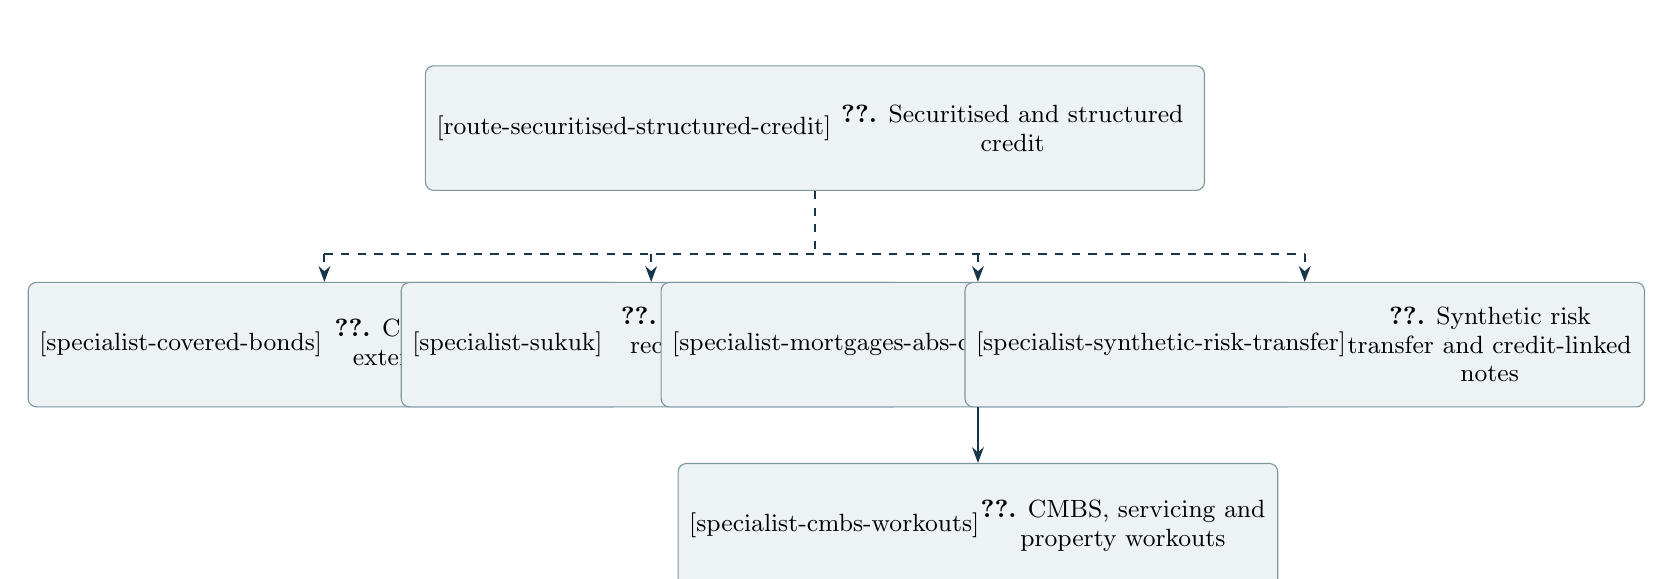
\begin{tikzpicture}[x=1cm,y=1cm]
\node[pathnode] (securitised-structured-credit) at (6.23,0) {\MeasurePathNode{4.6cm}{\textbf{\ref*{route-securitised-structured-credit}.} Securitised and structured credit}\hyperref[route-securitised-structured-credit]{\parbox[c][\pathnodeheight][c]{4.6cm}{\centering \textbf{\ref*{route-securitised-structured-credit}.} Securitised and structured credit}}};
\node[pathnode] (covered-bonds) at (0.00,-2.75) {\MeasurePathNode{3.65cm}{\textbf{\ref*{specialist-covered-bonds}.} Covered bonds and extendable maturity}\hyperref[specialist-covered-bonds]{\parbox[c][\pathnodeheight][c]{3.65cm}{\centering \textbf{\ref*{specialist-covered-bonds}.} Covered bonds and extendable maturity}}};
\node[pathnode] (sukuk) at (4.15,-2.75) {\MeasurePathNode{3.65cm}{\textbf{\ref*{specialist-sukuk}.} Sukuk: ownership, recourse and relative value}\hyperref[specialist-sukuk]{\parbox[c][\pathnodeheight][c]{3.65cm}{\centering \textbf{\ref*{specialist-sukuk}.} Sukuk: ownership, recourse and relative value}}};
\node[pathnode] (mortgages-abs-clo) at (8.30,-2.75) {\MeasurePathNode{3.65cm}{\textbf{\ref*{specialist-mortgages-abs-clo}.} Mortgages, ABS and CLO waterfalls}\hyperref[specialist-mortgages-abs-clo]{\parbox[c][\pathnodeheight][c]{3.65cm}{\centering \textbf{\ref*{specialist-mortgages-abs-clo}.} Mortgages, ABS and CLO waterfalls}}};
\node[pathnode] (synthetic-risk-transfer) at (12.45,-2.75) {\MeasurePathNode{3.65cm}{\textbf{\ref*{specialist-synthetic-risk-transfer}.} Synthetic risk transfer and credit-linked notes}\hyperref[specialist-synthetic-risk-transfer]{\parbox[c][\pathnodeheight][c]{3.65cm}{\centering \textbf{\ref*{specialist-synthetic-risk-transfer}.} Synthetic risk transfer and credit-linked notes}}};
\node[pathnode] (cmbs-workouts) at (8.30,-5.05) {\MeasurePathNode{3.65cm}{\textbf{\ref*{specialist-cmbs-workouts}.} CMBS, servicing and property workouts}\hyperref[specialist-cmbs-workouts]{\parbox[c][\pathnodeheight][c]{3.65cm}{\centering \textbf{\ref*{specialist-cmbs-workouts}.} CMBS, servicing and property workouts}}};
\draw[entryline] (securitised-structured-credit.south) -- (6.23,-1.60);
\draw[entryline] (0.00,-1.60) -- (12.45,-1.60);
\draw[entryarrow] (0.00,-1.60) -- (covered-bonds.north);
\draw[entryarrow] (4.15,-1.60) -- (sukuk.north);
\draw[entryarrow] (8.30,-1.60) -- (mortgages-abs-clo.north);
\draw[entryarrow] (12.45,-1.60) -- (synthetic-risk-transfer.north);
\draw[patharrow] (mortgages-abs-clo.south) -- (cmbs-workouts.north);
\end{tikzpicture}\end{center}
\textbf{Bring these foundations with you.}\begin{itemize}
\item \hyperref[specialist-corporate-credit-cds]{Corporate bonds and credit derivatives} --- needed by \hyperref[specialist-mortgages-abs-clo]{Mortgages, ABS and CLO waterfalls}.
\end{itemize}\hyperref[learning-map]{Return to the whole-guide DAG.}
\Needspace{12\baselineskip}
\subsection{Covered bonds and extendable maturity}\label{specialist-covered-bonds}
\textbf{Specialist pathway.} In \hyperref[route-securitised-structured-credit]{Securitised and structured credit}.

\textbf{Outcome.} Model issuer and cover-pool recourse, replacement assets, encumbrance and payment extension.

\textbf{Prerequisites.} Securitised and structured credit; bond cash flows, credit loss, discounting and option exercise.

\textbf{Review first.} \hyperref[route-securitised-structured-credit]{Securitised and structured credit}.

\textbf{Required readings, in order}
\begin{enumerate}\raggedright
\Needspace{5\baselineskip}\item \href{institutional_quantitative_finance_reading_list.pdf\#depth-covered-eu-directive}{European Union, Directive (EU) 2019/2162 on covered bonds}\CataloguePage{246}\NoteKey{depth-covered-eu-directive}\par \textbf{Legal claim.} Separate dual recourse, pool segregation and extension triggers under the selected EU framework.
\Needspace{5\baselineskip}\item \href{institutional_quantitative_finance_reading_list.pdf\#depth-covered-ccf-softbullet}{CCF Soci\'et\'e de Financement de l'Habitat, Base Prospectus, Soft Bullet Covered Bonds provisions}\CataloguePage{247}\NoteKey{depth-covered-ccf-softbullet}\par \textbf{Contract mechanics.} Read the actual programme extension clause, then identify issue-specific final terms.
\Needspace{5\baselineskip}\item \href{institutional_quantitative_finance_reading_list.pdf\#depth-covered-tasche-dual}{Dirk Tasche, Fitting a Distribution to Value-at-Risk and Expected Shortfall, with an Application to Covered Bonds; author preprint}\CataloguePage{246}\NoteKey{depth-covered-tasche-dual}\par \textbf{Loss model.} Compare one- and two-asset identification of issuer and cover-pool loss.
\Needspace{5\baselineskip}\item \href{institutional_quantitative_finance_reading_list.pdf\#depth-covered-kenyon-pricing}{Chris Kenyon, Pricing Covered Bonds}\CataloguePage{246}\NoteKey{depth-covered-kenyon-pricing}\par \textbf{Valuation.} Add replacement-pool and issuer-liquidity assumptions to a pricing model.
\Needspace{5\baselineskip}\item \href{institutional_quantitative_finance_reading_list.pdf\#depth-covered-credit-spread}{Marcel Prokopczuk, Jan B. Siewert and Volker Vonhoff, Credit Risk in Covered Bonds}\CataloguePage{246}\NoteKey{depth-covered-credit-spread}\par \textbf{Empirical comparison.} Assess the historical German spread evidence with its sample and liquidity controls.
\Needspace{5\baselineskip}\item \href{institutional_quantitative_finance_reading_list.pdf\#depth-covered-cashflow-monitor}{S\&P Global Ratings, Credit Rating Model: Covered Bond Monitor; Methodology for Rating Covered Bonds}\CataloguePage{246}\NoteKey{depth-covered-cashflow-monitor}\par \textbf{Cash-flow stress.} Separate rating stresses from fair-value inputs and refinancing execution.
\Needspace{5\baselineskip}\item \href{institutional_quantitative_finance_reading_list.pdf\#depth-covered-eba-review}{European Banking Authority, Advice on the Review of the EU Covered Bond Framework}\CataloguePage{247}\NoteKey{depth-covered-eba-review}\par \textbf{Recent framework review.} Distinguish supervisory advice from enacted changes.
\end{enumerate}
\Needspace{5\baselineskip}\textbf{Checkpoint.} Make separate issuer and cover-pool balance sheets. Trace scheduled and extended payments for a hypothetical CCF issue using explicitly selected final terms or labelled assumptions. Stress issuer default, pool loss, replacement assets and refinancing cost; compare expected loss with timing-sensitive present value. Reconcile which losses dual recourse covers and which liquidity gaps remain. Compare APS 121 before applying the exercise in Australia.

\textbf{Optional branches.} \href{institutional_quantitative_finance_reading_list.pdf\#depth-covered-apra}{Compare Australian prudential implementation.}\BranchPage{247} \href{institutional_quantitative_finance_reading_list.pdf\#depth-covered-encumbrance}{Assess unsecured-creditor costs of encumbrance.}\BranchPage{247}
\par{\small \hyperref[learning-map]{Learning pathway DAG} \textbar{} \hyperref[route-securitised-structured-credit]{Section overview} \textbar{} \hyperref[map-securitised-structured-credit]{Section DAG}\NoteKey{covered-bonds}}
\Needspace{12\baselineskip}
\subsection{Sukuk: ownership, recourse and relative value}\label{specialist-sukuk}
\textbf{Specialist pathway.} In \hyperref[route-securitised-structured-credit]{Securitised and structured credit}.

\textbf{Outcome.} Trace legal cash-flow rights and default outcomes before comparing sukuk with conventional debt.

\textbf{Prerequisites.} Securitised and structured credit; bond cash flows, credit loss, discounting and option exercise.

\textbf{Review first.} \hyperref[route-securitised-structured-credit]{Securitised and structured credit}.

\textbf{Required readings, in order}
\begin{enumerate}\raggedright
\Needspace{5\baselineskip}\item \href{institutional_quantitative_finance_reading_list.pdf\#depth-sukuk-ifsb19}{Islamic Financial Services Board, IFSB-19: Guiding Principles on Disclosure Requirements for Islamic Capital Market Products}\CataloguePage{250}\NoteKey{depth-sukuk-ifsb19}\par \textbf{Disclosure and structure.} Identify ownership, recourse, servicing and payment disclosures.
\Needspace{5\baselineskip}\item \href{institutional_quantitative_finance_reading_list.pdf\#depth-sukuk-imf-asset}{International Monetary Fund staff, Islamic Finance, Consumer Protection, and Financial Stability}\CataloguePage{250}\NoteKey{depth-sukuk-imf-asset}\par \textbf{Mechanism.} Distinguish asset-based from asset-backed transactions and true-sale questions.
\Needspace{5\baselineskip}\item \href{institutional_quantitative_finance_reading_list.pdf\#depth-sukuk-default-cases}{Sajjad Zaheer and Sweder van Wijnbergen, Sukuk Defaults: On Distress Resolution in Islamic Finance}\CataloguePage{250}\NoteKey{depth-sukuk-default-cases}\par \textbf{Default evidence.} Study selected enforcement failures without treating cases as a default-rate panel.
\Needspace{5\baselineskip}\item \href{institutional_quantitative_finance_reading_list.pdf\#depth-sukuk-primary-spreads}{Yusuf Ayturk, Mehmet Asutay and Ercument Aksak, What Explains Corporate Sukuk Primary Market Spreads?; author-university record}\CataloguePage{250}\NoteKey{depth-sukuk-primary-spreads}\par \textbf{Historical pricing.} Assess the international issuance spread model and limited sample.
\Needspace{5\baselineskip}\item \href{institutional_quantitative_finance_reading_list.pdf\#depth-sukuk-matched-pricing}{Nawaf Almaskati, Sukuk versus Bonds: New Evidence from the Primary Market}\CataloguePage{250}\NoteKey{depth-sukuk-matched-pricing}\par \textbf{Comparator design.} Test whether matched bonds separate structure from issuer and maturity.
\Needspace{5\baselineskip}\item \href{institutional_quantitative_finance_reading_list.pdf\#depth-sukuk-ifsb23}{Islamic Financial Services Board, IFSB-23: Revised Capital Adequacy Standard for Institutions Offering Islamic Financial Services (Banking Segment), especially \S6}\CataloguePage{250}\NoteKey{depth-sukuk-ifsb23}\par \textbf{Capital treatment.} Separate standard recommendations from local implementation.
\Needspace{5\baselineskip}\item \href{institutional_quantitative_finance_reading_list.pdf\#depth-sukuk-ifsb2025}{Islamic Financial Services Board, Islamic Financial Services Industry Stability Report 2025}\CataloguePage{251}\NoteKey{depth-sukuk-ifsb2025}\par \textbf{Market context.} Use the dated structure mix and data coverage to frame the opportunity set.
\Needspace{5\baselineskip}\item \href{institutional_quantitative_finance_reading_list.pdf\#w5-azmat-skully-brown}{Saad Azmat, Michael Skully and Kym Brown, ``The (little) difference that makes all the difference between Islamic and conventional bonds''}\CataloguePage{251}\NoteKey{w5-azmat-skully-brown}\par \textbf{Structures.} Separate asset-based from asset-backed sukuk economics.
\Needspace{5\baselineskip}\item \href{institutional_quantitative_finance_reading_list.pdf\#w5-godlewski-sukuk-stock}{Christophe J. Godlewski, Rima Turk-Ariss and Laurent Weill, ``Sukuk vs. conventional bonds: A stock market perspective''}\CataloguePage{251}\NoteKey{w5-godlewski-sukuk-stock}\par \textbf{Evidence.} See how equity markets react to sukuk issuance.
\end{enumerate}
\Needspace{5\baselineskip}\textbf{Checkpoint.} Draw the originator, SPV, assets, servicing, purchase undertaking and certificate-holder claims for one sourced issue. Reconcile normal distributions and default/enforcement cash flows, ownership and governing law; otherwise label the structure hypothetical. Build a conventional-bond comparison matched on issuer, currency, maturity, seniority and liquidity. Separate price effects from tax, investor segmentation and Sharia-board decisions. Identify missing issue documents and prices before making an executable-value claim.

\textbf{Optional branches.} \href{institutional_quantitative_finance_reading_list.pdf\#w5-klein-weill-why-sukuk}{Ask why firms choose sukuk.}\BranchPage{251} \href{institutional_quantitative_finance_reading_list.pdf\#w5-paltrinieri-sukuk-review}{Map the sukuk literature.}\BranchPage{251} \href{institutional_quantitative_finance_reading_list.pdf\#w5-aaoifi-standards}{Read the AAOIFI sukuk standard.}\BranchPage{251}
\par{\small \hyperref[learning-map]{Learning pathway DAG} \textbar{} \hyperref[route-securitised-structured-credit]{Section overview} \textbar{} \hyperref[map-securitised-structured-credit]{Section DAG}\NoteKey{sukuk}}
\Needspace{12\baselineskip}
\subsection{Mortgages, ABS and CLO waterfalls}\label{specialist-mortgages-abs-clo}
\textbf{Specialist pathway.} In \hyperref[route-securitised-structured-credit]{Securitised and structured credit}.

\textbf{Outcome.} Model collateral cash flows, prepayment or default, servicing and tranche allocation for several securitisation forms.

\textbf{Prerequisites.} Corporate bonds and credit derivatives; amortisation, option-adjusted spreads and legal seniority.

\textbf{Review first.} \hyperref[route-securitised-structured-credit]{Securitised and structured credit}; \hyperref[specialist-corporate-credit-cds]{Corporate bonds and credit derivatives}.

\textbf{Required readings, in order}
\begin{enumerate}\raggedright
\Needspace{5\baselineskip}\item \href{institutional_quantitative_finance_reading_list.pdf\#gap-sec-prepayment-valuation}{Eduardo S. Schwartz and Walter N. Torous, Prepayment and the Valuation of Mortgage-Backed Securities}\CataloguePage{255}\NoteKey{gap-sec-prepayment-valuation}\par \textbf{Valuation.} Introduce mortgage prepayment as borrower optionality.
\Needspace{5\baselineskip}\item \href{institutional_quantitative_finance_reading_list.pdf\#gap-sec-mbs-oas-chapter}{Matthew Dyer, Valuing and Analyzing Mortgage-Backed and Asset-Backed Securities}\CataloguePage{255}\NoteKey{gap-sec-mbs-oas-chapter}\par \textbf{Valuation.} Price mortgage cash flows across interest-rate paths.
\Needspace{5\baselineskip}\item \href{institutional_quantitative_finance_reading_list.pdf\#exp-vickery-wright-tba-mbs}{James Vickery and Joshua Wright, TBA Trading and Liquidity in the Agency MBS Market; 2013 full EPR issue}\CataloguePage{255}\NoteKey{exp-vickery-wright-tba-mbs}\par \textbf{Mechanics.} Understand TBA delivery and agency MBS market structure.
\Needspace{5\baselineskip}\item \href{institutional_quantitative_finance_reading_list.pdf\#gap-sec-fannie-loan-data}{Fannie Mae, Fannie Mae Single-Family Loan Performance Data; Fannie Mae Data Dynamics access route}\CataloguePage{256}\NoteKey{gap-sec-fannie-loan-data}\par \textbf{Data.} Build loan cohorts with correct reporting and revision semantics.
\Needspace{5\baselineskip}\item \href{institutional_quantitative_finance_reading_list.pdf\#gap-sec-umbs-prepay-monitor}{Federal Housing Finance Agency, Prepayment Monitoring Report}\CataloguePage{256}\NoteKey{gap-sec-umbs-prepay-monitor}\par \textbf{Evidence.} Compare modelled speeds with official observed agency performance.
\Needspace{5\baselineskip}\item \href{institutional_quantitative_finance_reading_list.pdf\#depth-sec-stacr-reference}{Freddie Mac, Single-Family Credit Risk Transfer Handbook and Reference Pool Disclosure File Layouts}\CataloguePage{257}\NoteKey{depth-sec-stacr-reference}\par \textbf{Mechanics.} Trace how agency credit risk is transferred to investors.
\Needspace{5\baselineskip}\item \href{institutional_quantitative_finance_reading_list.pdf\#depth-sec-auto-waterfall}{Volkswagen Auto Loan Enhanced Trust 2025-2, SEC-filed prospectus}\CataloguePage{260}\NoteKey{depth-sec-auto-waterfall}\par \textbf{Mechanics.} Follow a consumer ABS prospectus through monthly priorities and triggers.
\Needspace{5\baselineskip}\item \href{institutional_quantitative_finance_reading_list.pdf\#gap-sec-abs-asset-disclosure}{U.S. Securities and Exchange Commission, Asset-Backed Securities Disclosure and Registration, Regulation AB II; SEC adoption summary}\CataloguePage{257}\NoteKey{gap-sec-abs-asset-disclosure}\par \textbf{Data.} Use the deal's asset and servicing disclosures for loan-level assumptions.
\Needspace{5\baselineskip}\item \href{institutional_quantitative_finance_reading_list.pdf\#depth-sec-clo-indent}{Carlyle Direct Lending CLO 2024-1, Executed Indenture}\CataloguePage{262}\NoteKey{depth-sec-clo-indent}\par \textbf{Mechanics.} Read CLO diversion tests and tranche priority from an indenture.
\Needspace{5\baselineskip}\item \href{institutional_quantitative_finance_reading_list.pdf\#depth-sec-clo-2026-surveillance}{Arbor Realty Trust, First-Quarter 2026 Form 10-Q, CLO Compliance Tests}\CataloguePage{262}\NoteKey{depth-sec-clo-2026-surveillance}\par \textbf{Evidence.} Contrast CRE CLO surveillance ratios with the direct-lending indenture; do not join them as one deal.
\Needspace{5\baselineskip}\item \href{institutional_quantitative_finance_reading_list.pdf\#depth-sec-basel-waterfall}{Basel Committee on Banking Supervision, Basel Framework, CRE40 Securitisation: General Provisions}\CataloguePage{257}\NoteKey{depth-sec-basel-waterfall}\par \textbf{Valuation.} Check how tranche attachment and loss allocation alter risk.
\Needspace{5\baselineskip}\item \href{institutional_quantitative_finance_reading_list.pdf\#gap-sec-specified-pool-stress}{Jiakai Chen, Haoyang Liu, David Rubio, Asani Sarkar and Zhaogang Song, MBS Market Dysfunctions in the Time of COVID-19; Related New York Fed Staff Report 933, revised September 2026}\CataloguePage{256}\NoteKey{gap-sec-specified-pool-stress}\par \textbf{Implementation.} Stress pool selection and execution basis against generic MBS pricing.
\end{enumerate}
\Needspace{5\baselineskip}\textbf{Checkpoint.} Build small cash-flow models for one agency MBS cohort, one public auto ABS and one CLO indenture. Reconcile collateral cash to note interest, principal, reserve and residual each month; stress rates, prepayments, losses and trigger breaches. Keep the CLO waterfall illustrative unless same-deal collateral and trustee reports are obtained; the separate CRE CLO disclosure cannot validate a direct-lending CLO model. State remaining licensed-data and document gaps.

\textbf{Optional branches.} \href{institutional_quantitative_finance_reading_list.pdf\#wide-davidson-levin}{Read a mortgage valuation-model text.}\BranchPage{257} \href{institutional_quantitative_finance_reading_list.pdf\#wide-fuster-mbs-review}{Survey agency MBS markets.}\BranchPage{258} \href{institutional_quantitative_finance_reading_list.pdf\#wide-benmelech-clo}{Test adverse selection in CLOs.}\BranchPage{262} \href{institutional_quantitative_finance_reading_list.pdf\#w2-peristiani-santos-clo}{Study bank-affiliated CLO manager trading.}\BranchPage{262} \href{institutional_quantitative_finance_reading_list.pdf\#w2-benmelech-autos}{See the funding role of auto ABS in 2008.}\BranchPage{261} \href{institutional_quantitative_finance_reading_list.pdf\#w5-griffin-nickerson-clo}{Check CLO tranche ratings against collateral.}\BranchPage{263} \href{institutional_quantitative_finance_reading_list.pdf\#w5-benmelech-dlugosz-alchemy}{See how CDO ratings were engineered.}\BranchPage{262} \href{institutional_quantitative_finance_reading_list.pdf\#w5-irani-shadow-banking}{Trace loans from banks to nonbank holders.}\BranchPage{263} \href{institutional_quantitative_finance_reading_list.pdf\#w5-adams-einav-levin}{Study subprime auto-loan selection.}\BranchPage{261}
\par{\small \hyperref[learning-map]{Learning pathway DAG} \textbar{} \hyperref[route-securitised-structured-credit]{Section overview} \textbar{} \hyperref[map-securitised-structured-credit]{Section DAG}\NoteKey{mortgages-abs-clo}}
\Needspace{12\baselineskip}
\subsection{Synthetic risk transfer and credit-linked notes}\label{specialist-synthetic-risk-transfer}
\textbf{Specialist pathway.} In \hyperref[route-securitised-structured-credit]{Securitised and structured credit}.

\textbf{Outcome.} Connect reference-pool losses, tranche protection and bank capital with counterparty and financing risk.

\textbf{Prerequisites.} Securitised and structured credit; bond cash flows, credit loss, discounting and option exercise.

\textbf{Review first.} \hyperref[route-securitised-structured-credit]{Securitised and structured credit}.

\textbf{Required readings, in order}
\begin{enumerate}\raggedright
\Needspace{5\baselineskip}\item \href{institutional_quantitative_finance_reading_list.pdf\#depth-srt-bis-mechanics}{Bank for International Settlements, The Rise and Risks of Synthetic Risk Transfers}\CataloguePage{252}\NoteKey{depth-srt-bis-mechanics}\par \textbf{Structures.} Compare direct and SPV credit-linked notes with unfunded protection.
\Needspace{5\baselineskip}\item \href{institutional_quantitative_finance_reading_list.pdf\#depth-srt-bcbs2026}{Basel Committee on Banking Supervision, Synthetic Risk Transfers}\CataloguePage{251}\NoteKey{depth-srt-bcbs2026}\par \textbf{Supervisory evidence.} Assess current survey findings and limits of regulatory risk-transfer recognition.
\Needspace{5\baselineskip}\item \href{institutional_quantitative_finance_reading_list.pdf\#depth-srt-fed-regq}{Board of Governors of the Federal Reserve System, Regulation Q Frequently Asked Questions: Credit-Linked Notes and Synthetic Securitisation}\CataloguePage{252}\NoteKey{depth-srt-fed-regq}\par \textbf{Jurisdictional treatment.} Trace the US direct-note and SPV distinctions without assuming automatic relief.
\Needspace{5\baselineskip}\item \href{institutional_quantitative_finance_reading_list.pdf\#depth-srt-ecb-microdata}{Alex Osberghaus and Glenn Schepens, Synthetic, but How Much Risk Transfer?}\CataloguePage{252}\NoteKey{depth-srt-ecb-microdata}\par \textbf{Empirical evidence.} Interpret bank-level findings while recognising restricted underlying observations.
\Needspace{5\baselineskip}\item \href{institutional_quantitative_finance_reading_list.pdf\#depth-sec-basel-waterfall}{Basel Committee on Banking Supervision, Basel Framework, CRE40 Securitisation: General Provisions}\CataloguePage{257}\NoteKey{depth-sec-basel-waterfall}\par \textbf{Due diligence.} Use structural diligence to identify loss-allocation and documentation requirements.
\Needspace{5\baselineskip}\item \href{institutional_quantitative_finance_reading_list.pdf\#w2-imf-srt-2025}{Fabio Cortes, Fernando Fernandez Dionis, Yi Li, Andres Ramirez and Mengxue Zhang (authors as listed by IMF), ``Recycling Risk: Synthetic Risk Transfers''}\CataloguePage{252}\NoteKey{w2-imf-srt-2025}\par \textbf{Evidence.} Review SRT growth, structures and investors across jurisdictions.
\Needspace{5\baselineskip}\item \href{institutional_quantitative_finance_reading_list.pdf\#w2-eba-srt-2020}{European Banking Authority, ``Report on significant risk transfer in securitisation''}\CataloguePage{252}\NoteKey{w2-eba-srt-2020}\par \textbf{Regulation.} Apply supervisory significant-risk-transfer tests.
\Needspace{5\baselineskip}\item \href{institutional_quantitative_finance_reading_list.pdf\#w5-coval-jurek-stafford}{Joshua Coval, Jakub Jurek and Erik Stafford, ``The Economics of Structured Finance''}\CataloguePage{253}\NoteKey{w5-coval-jurek-stafford}\par \textbf{Foundations.} See how tranching concentrates systematic risk.
\end{enumerate}
\Needspace{5\baselineskip}\textbf{Checkpoint.} For an explicitly hypothetical pool, calculate attachment, exhaustion, realised loss allocation, amortisation and maturity mismatch. Add investor leverage, collateral and counterparty-default branches. Separate the protection buyer's accounting, regulatory capital and economic risk reduction from the investor's return. A public survey cannot identify a live deal: list the executed protection agreement, eligibility/replenishment rules, reference-pool history and financing terms required for a transaction valuation.

\textbf{Optional branches.} \href{institutional_quantitative_finance_reading_list.pdf\#w5-gorton-pennacchi-loan-sales}{Study incentives in loan sales.}\BranchPage{252} \href{institutional_quantitative_finance_reading_list.pdf\#w5-parlour-winton}{Compare loan sales with CDS protection.}\BranchPage{253} \href{institutional_quantitative_finance_reading_list.pdf\#w5-duffie-crt-bis}{Review credit-risk-transfer stability issues.}\BranchPage{252}
\par{\small \hyperref[learning-map]{Learning pathway DAG} \textbar{} \hyperref[route-securitised-structured-credit]{Section overview} \textbar{} \hyperref[map-securitised-structured-credit]{Section DAG}\NoteKey{synthetic-risk-transfer}}
\Needspace{12\baselineskip}
\subsection{CMBS, servicing and property workouts}\label{specialist-cmbs-workouts}
\textbf{Specialist pathway.} In \hyperref[route-securitised-structured-credit]{Securitised and structured credit}.

\textbf{Outcome.} Reconcile commercial-property cash flows, servicing advances, workout rights and certificate distributions.

\textbf{Prerequisites.} Mortgages, ABS and CLO waterfalls; property NOI, debt-service coverage and legal payment priority.

\textbf{Review first.} \hyperref[route-securitised-structured-credit]{Securitised and structured credit}; \hyperref[specialist-mortgages-abs-clo]{Mortgages, ABS and CLO waterfalls}.

\textbf{Required readings, in order}
\begin{enumerate}\raggedright
\Needspace{5\baselineskip}\item \href{institutional_quantitative_finance_reading_list.pdf\#depth-geltner-book-2026}{David M. Geltner, Norman G. Miller, Alex Van De Minne, Piet Eichholtz, Thies Lindenthal and Lily Shen, Commercial Real Estate Analysis for Investment, Finance, and Development}\CataloguePage{419}\NoteKey{depth-geltner-book-2026}\par \textbf{Valuation.} Build property cash flows and refinancing scenarios before pricing securitised claims.
\Needspace{5\baselineskip}\item \href{institutional_quantitative_finance_reading_list.pdf\#gap-sec-cmbs-liquidity-model}{Peimin Chen, Igor Kozhanov, Peng Liu and Chunchi Wu, Commercial Mortgage-Backed Security Pricing with Real Estate Liquidity Risk}\CataloguePage{256}\NoteKey{gap-sec-cmbs-liquidity-model}\par \textbf{Valuation.} Connect property sale liquidity, default timing and structural credit risk.
\Needspace{5\baselineskip}\item \href{institutional_quantitative_finance_reading_list.pdf\#depth-sec-cmbs-2025-deal}{BBCMS Mortgage Trust 2025-C39, SEC-filed structural and collateral term sheet}\CataloguePage{258}\NoteKey{depth-sec-cmbs-2025-deal}\par \textbf{Mechanics.} Distinguish preliminary terms, definitive agreements, control rights and monthly distributions.
\Needspace{5\baselineskip}\item \href{institutional_quantitative_finance_reading_list.pdf\#depth-sec-crefc-irp}{CRE Finance Council, Investor Reporting Package, Version 8.4}\CataloguePage{258}\NoteKey{depth-sec-crefc-irp}\par \textbf{Data.} Join property, loan, servicing and bond reports with dated field definitions.
\Needspace{5\baselineskip}\item \href{institutional_quantitative_finance_reading_list.pdf\#gap-sec-abs-asset-disclosure}{U.S. Securities and Exchange Commission, Asset-Backed Securities Disclosure and Registration, Regulation AB II; SEC adoption summary}\CataloguePage{257}\NoteKey{gap-sec-abs-asset-disclosure}\par \textbf{Data.} Trace asset disclosures and reporting timestamps to the selected deal.
\Needspace{5\baselineskip}\item \href{institutional_quantitative_finance_reading_list.pdf\#evidence-rithm-advances}{Rithm Capital, 2025 Form 10-K; filing PDF}\CataloguePage{257}\NoteKey{evidence-rithm-advances}\par \textbf{Evidence.} Study advance financing and recovery risk while retaining issuer-specific limits.
\Needspace{5\baselineskip}\item \href{institutional_quantitative_finance_reading_list.pdf\#re-gupta-office-2026}{Arpit Gupta, Vrinda Mittal, and Stijn Van Nieuwerburgh, Work from Home and the Office Real Estate Apocalypse}\CataloguePage{420}\NoteKey{re-gupta-office-2026}\par \textbf{Evidence.} Challenge office-value and refinancing assumptions using recent structural evidence.
\Needspace{5\baselineskip}\item \href{institutional_quantitative_finance_reading_list.pdf\#w2-crosignani-prazad}{Matteo Crosignani and Saketh Prazad, ``Extend-and-Pretend in the U.S. CRE Market''}\CataloguePage{259}\NoteKey{w2-crosignani-prazad}\par \textbf{Evidence.} Assess the extend-and-pretend hypothesis for CRE loans.
\Needspace{5\baselineskip}\item \href{institutional_quantitative_finance_reading_list.pdf\#w2-glancy-pretend-amend}{David Glancy, ``Pretend or Amend? On Evergreening in CRE''}\CataloguePage{259}\NoteKey{w2-glancy-pretend-amend}\par \textbf{Counter-evidence.} Compare evidence that extensions mostly address temporary frictions.
\end{enumerate}
\Needspace{5\baselineskip}\textbf{Checkpoint.} Use the C39 March 2026 filing/exhibit references to distinguish certificate interest, principal and fees from arrears, advances and recoveries. Check the reported interest-plus-principal distribution total, identifying the indexed evidence boundary. Then model an extension and property sale only with explicitly sourced or assumed inputs. A replicated waterfall requires full definitive PSA/424B2, Exhibit 99.1, ABS-EE collateral and advances/fees reconciliation; the selected monthly figures alone do not establish it.

\textbf{Optional branches.} \href{institutional_quantitative_finance_reading_list.pdf\#wide-titman-tsyplakov-cmbs}{Relate originator incentives to CMBS risk.}\BranchPage{258} \href{institutional_quantitative_finance_reading_list.pdf\#wide-stanton-wallace-cmbs}{Study CMBS subordination and ratings inflation.}\BranchPage{259} \href{institutional_quantitative_finance_reading_list.pdf\#w2-an-deng-gabriel}{Price adverse selection in conduit CMBS.}\BranchPage{259} \href{institutional_quantitative_finance_reading_list.pdf\#w2-ghent-torous-valkanov}{Survey CRE as an asset class.}\BranchPage{259} \href{institutional_quantitative_finance_reading_list.pdf\#w6-griffin-priest-cmbs}{Test CMBS income overstatement against COVID defaults.}\BranchPage{260} \href{institutional_quantitative_finance_reading_list.pdf\#w6-black-krainer-nichols}{Compare workouts of securitised and portfolio loans.}\BranchPage{259} \href{institutional_quantitative_finance_reading_list.pdf\#w6-glancy-segmentation}{See CRE lender segmentation.}\BranchPage{260} \href{institutional_quantitative_finance_reading_list.pdf\#w6-ambrose-sanders-cmbs}{Model CMBS prepayment and default.}\BranchPage{259}
\par{\small \hyperref[learning-map]{Learning pathway DAG} \textbar{} \hyperref[route-securitised-structured-credit]{Section overview} \textbar{} \hyperref[map-securitised-structured-credit]{Section DAG}\NoteKey{cmbs-workouts}}
\clearpage
\section{Systematic equities}\label{route-systematic-equities}
\label{route-2}
\textbf{Learning sequence.} Start from factor premia, statistical arbitrage, investor flows and fundamental valuation; then study short-selling, option, insider and retail-flow signals, combine signals into a risk-controlled long–short portfolio, and finish with corporate events and merger arbitrage.

\textbf{Section goals.} Across its pathways, this section teaches you to:
\begin{itemize}[leftmargin=1.4em,itemsep=0pt,topsep=1pt]
\item construct and time factor premia and measure their crash risk (\hyperref[specialist-equity-factor-premia]{\ref*{specialist-equity-factor-premia}})
\item design residual mean-reversion and pairs strategies (\hyperref[specialist-statistical-arbitrage]{\ref*{specialist-statistical-arbitrage}})
\item estimate demand elasticities, flow-driven price impact and the effects of passive ownership (\hyperref[specialist-demand-flows-passive]{\ref*{specialist-demand-flows-passive}})
\item turn financial statements into valuation and accounting signals (\hyperref[specialist-equity-events-fundamentals]{\ref*{specialist-equity-events-fundamentals}})
\item test short-selling, option, insider and retail-flow signals (\hyperref[specialist-equity-trader-signals]{\ref*{specialist-equity-trader-signals}})
\item combine signals into a neutral long--short portfolio with a matched risk model (\hyperref[specialist-equity-long-short-construction]{\ref*{specialist-equity-long-short-construction}})
\item measure event returns and size merger-arbitrage positions (\hyperref[specialist-equity-event-driven]{\ref*{specialist-equity-event-driven}})
\end{itemize}
\textbf{Overview outcome.} Rebuild a stock characteristic from point-in-time inputs and judge whether its return survives weighting choices, the exclusion of microcaps, trading costs and the move from the original sample to post-publication and forward-only periods.

\textbf{Prerequisites.} Common toolkit; equity returns, corporate actions, survivorship and basic factor regressions.

\textbf{Review first.} \hyperref[route-common-toolkit]{Common toolkit}.

\textbf{Required readings, in order}
\begin{enumerate}\raggedright
\Needspace{5\baselineskip}\item \href{institutional_quantitative_finance_reading_list.pdf\#alpha-ff1993}{Eugene Fama and Kenneth French, ``Common Risk Factors in the Returns on Stocks and Bonds''}\CataloguePage{192}\NoteKey{alpha-ff1993}\par Start with the factor benchmark against which a proposed stock signal must be compared.
\Needspace{5\baselineskip}\item \href{institutional_quantitative_finance_reading_list.pdf\#s7-jegadeesh}{Narasimhan Jegadeesh and Sheridan Titman, ``Returns to Buying Winners and Selling Losers''}\CataloguePage{192}\NoteKey{s7-jegadeesh}\par Study a canonical anomaly and the choices needed to turn a return spread into a portfolio.
\Needspace{5\baselineskip}\item \href{institutional_quantitative_finance_reading_list.pdf\#exp-open-source-ap}{Andrew Y. Chen and Tom Zimmermann, Open Source Cross-Sectional Asset Pricing; Author project code}\CataloguePage{87}\NoteKey{exp-open-source-ap}\par Reconstruct definitions, reporting lags, breakpoints and weighting from reusable characteristic code.
\Needspace{5\baselineskip}\item \href{institutional_quantitative_finance_reading_list.pdf\#exp-replicating-anomalies}{Kewei Hou, Chen Xue, and Lu Zhang, Replicating Anomalies}\CataloguePage{87}\NoteKey{exp-replicating-anomalies}\par Test how standardized constructions and microcap exposure reduce apparent anomaly evidence.
\Needspace{5\baselineskip}\item \href{institutional_quantitative_finance_reading_list.pdf\#exp-jkp-replication}{Theis Ingerslev Jensen, Bryan Kelly, and Lasse Heje Pedersen, Is There a Replication Crisis in Finance?; Project data and documentation}\CataloguePage{87}\NoteKey{exp-jkp-replication}\par Compare a different replication design and global evidence before declaring a factor either real or refuted.
\Needspace{5\baselineskip}\item \href{institutional_quantitative_finance_reading_list.pdf\#exp-trading-cost-anomalies}{Robert Novy-Marx and Mihail Velikov, A Taxonomy of Anomalies and Their Trading Costs}\CataloguePage{87}\NoteKey{exp-trading-cost-anomalies}\par Move from gross return spreads to turnover-aware entry, hold and exit decisions.
\Needspace{5\baselineskip}\item \href{institutional_quantitative_finance_reading_list.pdf\#exp-publication-decay}{R. David McLean and Jeffrey Pontiff, Does Academic Research Destroy Stock Return Predictability?}\CataloguePage{87}\NoteKey{exp-publication-decay}\par Distinguish original-sample performance from later decay and crowding after disclosure.
\Needspace{5\baselineskip}\item \href{institutional_quantitative_finance_reading_list.pdf\#exp-implementable-frontier}{Theis Ingerslev Jensen, Bryan Kelly, Semyon Malamud, and Lasse Heje Pedersen, Machine Learning and the Implementable Efficient Frontier}\CataloguePage{53}\NoteKey{exp-implementable-frontier}\par Finish with a risk and trading-cost frontier; test desk-specific capacity, borrow and financing separately.
\end{enumerate}
\Needspace{5\baselineskip}\textbf{Checkpoint.} Rebuild two stock characteristics from point-in-time inputs. Report equal- and value-weighted results with and without microcaps, then net returns under turnover, borrow and impact assumptions; record original, postpublication and forward-only periods separately.

\textbf{Optional branches.} \href{institutional_quantitative_finance_reading_list.pdf\#section.10.2}{Add cash-flow valuation, ETF creation/redemption and transmission into underlying stocks.}\BranchPage{199} \href{institutional_quantitative_finance_reading_list.pdf\#section.3.5}{Add filing and news signals after the factor benchmark is stable.}\BranchPage{64} \href{institutional_quantitative_finance_reading_list.pdf\#latest-ai-asset-pricing-transformer}{Study a modern conditional SDF architecture after replication and implementability.}\BranchPage{53} \href{institutional_quantitative_finance_reading_list.pdf\#wide-bali-engle-murray}{Use a practical empirical asset-pricing manual.}\BranchPage{29} \href{institutional_quantitative_finance_reading_list.pdf\#s16-r06}{Read how equity long--short, quantitative and event-driven managers trade and where their returns come from.}\BranchPage{33}
\par\textbf{Continue in this section.} \hyperref[specialist-equity-factor-premia]{Equity factor premia, crashes and timing}; \hyperref[specialist-statistical-arbitrage]{Statistical arbitrage and short-horizon equity strategies}; \hyperref[specialist-demand-flows-passive]{Demand-based asset pricing, flows and passive investing}; \hyperref[specialist-equity-events-fundamentals]{Fundamental valuation and accounting signals}; \hyperref[specialist-equity-trader-signals]{Short-selling, option, insider and retail-flow signals}; \hyperref[specialist-equity-long-short-construction]{Equity signal combination, risk models and long–short portfolios}; \hyperref[specialist-equity-event-driven]{Earnings, corporate events and merger arbitrage}.
\par{\small \hyperref[learning-map]{Learning pathway DAG} \textbar{} \hyperref[map-systematic-equities]{Section DAG}\NoteKey{systematic-equities}}
\clearpage
\subsection*{Systematic equities: pathway DAG}\phantomsection\label{map-systematic-equities}
\addcontentsline{toc}{subsection}{Systematic equities: pathway DAG}
Start with the section overview's readings, for orientation. Solid arrows show prerequisites within this section. Dashed connectors identify entry points with no further prerequisite in this section; the linked foundations below still apply. Follow the arrows for dependencies and the subsection numbers for reading order. Every node is clickable.
\begin{center}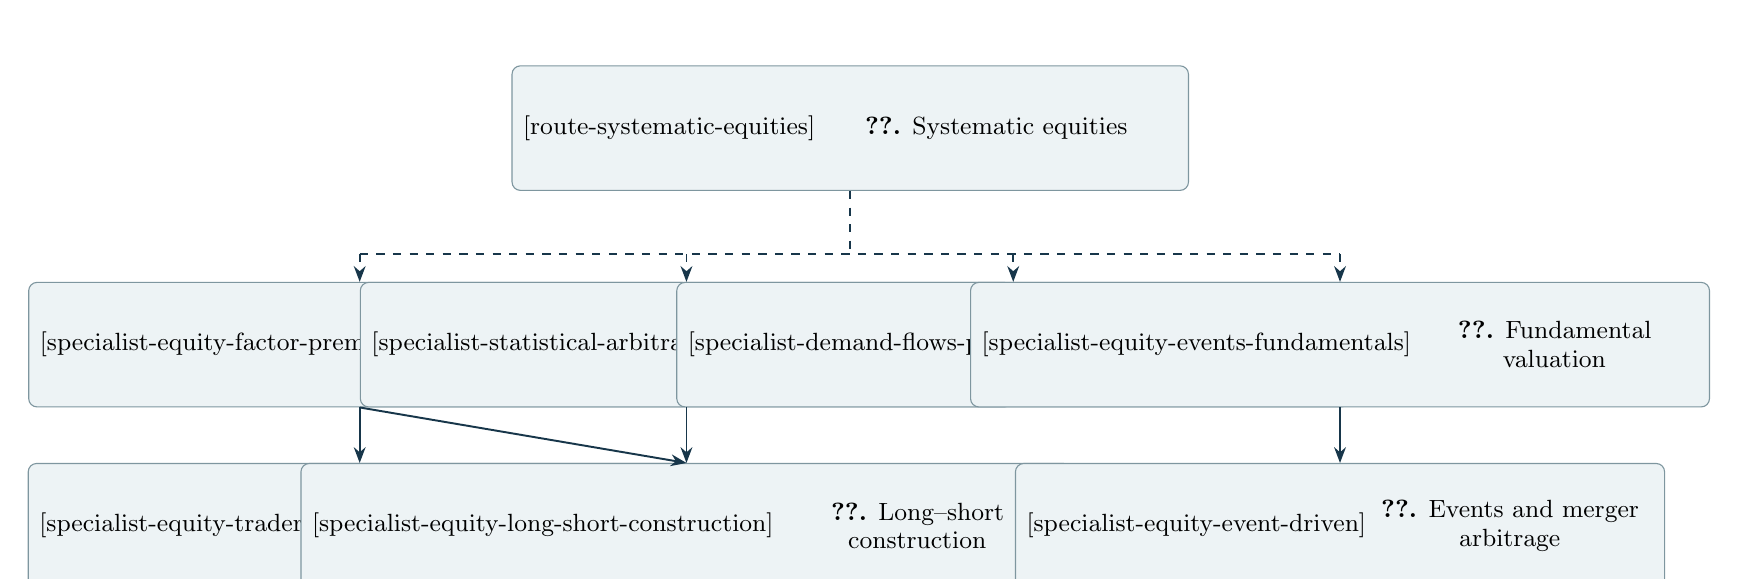
\begin{tikzpicture}[x=1cm,y=1cm]
\node[pathnode] (systematic-equities) at (6.23,0) {\MeasurePathNode{4.6cm}{\textbf{\ref*{route-systematic-equities}.} Systematic equities}\hyperref[route-systematic-equities]{\parbox[c][\pathnodeheight][c]{4.6cm}{\centering \textbf{\ref*{route-systematic-equities}.} Systematic equities}}};
\node[pathnode] (equity-factor-premia) at (0.00,-2.75) {\MeasurePathNode{3.65cm}{\textbf{\ref*{specialist-equity-factor-premia}.} Equity factor premia}\hyperref[specialist-equity-factor-premia]{\parbox[c][\pathnodeheight][c]{3.65cm}{\centering \textbf{\ref*{specialist-equity-factor-premia}.} Equity factor premia}}};
\node[pathnode] (statistical-arbitrage) at (4.15,-2.75) {\MeasurePathNode{3.65cm}{\textbf{\ref*{specialist-statistical-arbitrage}.} Statistical arbitrage}\hyperref[specialist-statistical-arbitrage]{\parbox[c][\pathnodeheight][c]{3.65cm}{\centering \textbf{\ref*{specialist-statistical-arbitrage}.} Statistical arbitrage}}};
\node[pathnode] (demand-flows-passive) at (8.30,-2.75) {\MeasurePathNode{3.65cm}{\textbf{\ref*{specialist-demand-flows-passive}.} Demand, flows and passive}\hyperref[specialist-demand-flows-passive]{\parbox[c][\pathnodeheight][c]{3.65cm}{\centering \textbf{\ref*{specialist-demand-flows-passive}.} Demand, flows and passive}}};
\node[pathnode] (equity-events-fundamentals) at (12.45,-2.75) {\MeasurePathNode{3.65cm}{\textbf{\ref*{specialist-equity-events-fundamentals}.} Fundamental valuation}\hyperref[specialist-equity-events-fundamentals]{\parbox[c][\pathnodeheight][c]{3.65cm}{\centering \textbf{\ref*{specialist-equity-events-fundamentals}.} Fundamental valuation}}};
\node[pathnode] (equity-trader-signals) at (0.00,-5.05) {\MeasurePathNode{3.65cm}{\textbf{\ref*{specialist-equity-trader-signals}.} Trader-flow signals}\hyperref[specialist-equity-trader-signals]{\parbox[c][\pathnodeheight][c]{3.65cm}{\centering \textbf{\ref*{specialist-equity-trader-signals}.} Trader-flow signals}}};
\node[pathnode] (equity-long-short-construction) at (4.15,-5.05) {\MeasurePathNode{3.65cm}{\textbf{\ref*{specialist-equity-long-short-construction}.} Long–short construction}\hyperref[specialist-equity-long-short-construction]{\parbox[c][\pathnodeheight][c]{3.65cm}{\centering \textbf{\ref*{specialist-equity-long-short-construction}.} Long–short construction}}};
\node[pathnode] (equity-event-driven) at (12.45,-5.05) {\MeasurePathNode{3.65cm}{\textbf{\ref*{specialist-equity-event-driven}.} Events and merger arbitrage}\hyperref[specialist-equity-event-driven]{\parbox[c][\pathnodeheight][c]{3.65cm}{\centering \textbf{\ref*{specialist-equity-event-driven}.} Events and merger arbitrage}}};
\draw[entryline] (systematic-equities.south) -- (6.23,-1.60);
\draw[entryline] (0.00,-1.60) -- (12.45,-1.60);
\draw[entryarrow] (0.00,-1.60) -- (equity-factor-premia.north);
\draw[entryarrow] (4.15,-1.60) -- (statistical-arbitrage.north);
\draw[entryarrow] (8.30,-1.60) -- (demand-flows-passive.north);
\draw[entryarrow] (12.45,-1.60) -- (equity-events-fundamentals.north);
\draw[patharrow] (equity-factor-premia.south) -- (equity-trader-signals.north);
\draw[patharrow] (equity-factor-premia.south) -- (equity-long-short-construction.north);
\draw[patharrow] (statistical-arbitrage.south) -- (equity-long-short-construction.north);
\draw[patharrow] (equity-events-fundamentals.south) -- (equity-event-driven.north);
\end{tikzpicture}\end{center}
\textbf{Bring these foundations with you.}\begin{itemize}
\item \hyperref[specialist-empirical-asset-pricing]{Empirical asset pricing: factor models and tests} --- needed by \hyperref[specialist-equity-factor-premia]{Equity factor premia}, \hyperref[specialist-demand-flows-passive]{Demand, flows and passive}, \hyperref[specialist-equity-event-driven]{Events and merger arbitrage}.
\item \hyperref[specialist-time-series-volatility]{Time-series econometrics and volatility forecasting} --- needed by \hyperref[specialist-statistical-arbitrage]{Statistical arbitrage}.
\item \hyperref[specialist-high-dimensional-estimation]{High-dimensional estimation, random matrices and heavy tails} --- needed by \hyperref[specialist-equity-long-short-construction]{Long–short construction}.
\end{itemize}\hyperref[learning-map]{Return to the whole-guide DAG.}
\Needspace{12\baselineskip}
\subsection{Equity factor premia, crashes and timing}\label{specialist-equity-factor-premia}
\textbf{Specialist pathway.} In \hyperref[route-systematic-equities]{Systematic equities}.

\textbf{Outcome.} Construct value, momentum, profitability, quality and low-risk factors, measure their crash risk and costs, and judge timing claims.

\textbf{Prerequisites.} Systematic equities overview and empirical asset pricing.

\textbf{Review first.} \hyperref[route-systematic-equities]{Systematic equities}; \hyperref[specialist-empirical-asset-pricing]{Empirical asset pricing: factor models and tests}.

\textbf{Required readings, in order}
\begin{enumerate}\raggedright
\Needspace{5\baselineskip}\item \href{institutional_quantitative_finance_reading_list.pdf\#alpha-ff1993}{Eugene Fama and Kenneth French, ``Common Risk Factors in the Returns on Stocks and Bonds''}\CataloguePage{192}\NoteKey{alpha-ff1993}\par \textbf{Evidence.} Start from size and value.
\Needspace{5\baselineskip}\item \href{institutional_quantitative_finance_reading_list.pdf\#wide-carhart}{Mark M. Carhart, ``On Persistence in Mutual Fund Performance''}\CataloguePage{109}\NoteKey{wide-carhart}\par \textbf{Evidence.} Add momentum in performance attribution.
\Needspace{5\baselineskip}\item \href{institutional_quantitative_finance_reading_list.pdf\#s7-jegadeesh}{Narasimhan Jegadeesh and Sheridan Titman, ``Returns to Buying Winners and Selling Losers''}\CataloguePage{192}\NoteKey{s7-jegadeesh}\par \textbf{Evidence.} Read the original momentum evidence.
\Needspace{5\baselineskip}\item \href{institutional_quantitative_finance_reading_list.pdf\#wide-novy-marx-profitability}{Robert Novy-Marx, ``The other side of value: The gross profitability premium''}\CataloguePage{193}\NoteKey{wide-novy-marx-profitability}\par \textbf{Evidence.} Add gross profitability.
\Needspace{5\baselineskip}\item \href{institutional_quantitative_finance_reading_list.pdf\#alpha-qmj}{Clifford Asness, Andrea Frazzini and Lasse Pedersen, ``Quality Minus Junk''}\CataloguePage{192}\NoteKey{alpha-qmj}\par \textbf{Evidence.} Build a broad quality factor from profitability, growth, safety and payout.
\Needspace{5\baselineskip}\item \href{institutional_quantitative_finance_reading_list.pdf\#wide-ff-five-factor}{Eugene F. Fama and Kenneth R. French, ``A five-factor asset pricing model''}\CataloguePage{28}\NoteKey{wide-ff-five-factor}\par \textbf{Evidence.} Compare five-factor redundancy.
\Needspace{5\baselineskip}\item \href{institutional_quantitative_finance_reading_list.pdf\#alpha-value}{Clifford Asness, Tobias Moskowitz and Lasse Heje Pedersen, ``Value and Momentum Everywhere'' (author copy)}\CataloguePage{192}\NoteKey{alpha-value}\par \textbf{Evidence.} See value and momentum across asset classes.
\Needspace{5\baselineskip}\item \href{institutional_quantitative_finance_reading_list.pdf\#wide-daniel-moskowitz-crashes}{Kent Daniel and Tobias J. Moskowitz, ``Momentum crashes''}\CataloguePage{193}\NoteKey{wide-daniel-moskowitz-crashes}\par \textbf{Evidence.} Measure momentum crash risk.
\Needspace{5\baselineskip}\item \href{institutional_quantitative_finance_reading_list.pdf\#wide-barroso-santa-clara}{Pedro Barroso and Pedro Santa-Clara, ``Momentum has its moments''}\CataloguePage{193}\NoteKey{wide-barroso-santa-clara}\par \textbf{Implementation.} Scale momentum by its volatility.
\Needspace{5\baselineskip}\item \href{institutional_quantitative_finance_reading_list.pdf\#alpha-bab}{Andrea Frazzini and Lasse Heje Pedersen, ``Betting Against Beta''}\CataloguePage{192}\NoteKey{alpha-bab}\par \textbf{Evidence.} Construct betting-against-beta.
\Needspace{5\baselineskip}\item \href{institutional_quantitative_finance_reading_list.pdf\#wide-ang-hodrick-ivol}{Andrew Ang, Robert J. Hodrick, Yuhang Xing and Xiaoyan Zhang, ``The Cross-Section of Volatility and Expected Returns''}\CataloguePage{193}\NoteKey{wide-ang-hodrick-ivol}\par \textbf{Evidence.} Study idiosyncratic-volatility returns.
\Needspace{5\baselineskip}\item \href{institutional_quantitative_finance_reading_list.pdf\#wide-israel-value-dead}{Ronen Israel, Kristoffer Laursen and Scott Richardson, ``Is (Systematic) Value Investing Dead?''}\CataloguePage{193}\NoteKey{wide-israel-value-dead}\par \textbf{Evidence.} Decompose the 2018--2020 value drawdown.
\Needspace{5\baselineskip}\item \href{institutional_quantitative_finance_reading_list.pdf\#wide-ehsani-linnainmaa}{Sina Ehsani and Juhani T. Linnainmaa, ``Factor Momentum and the Momentum Factor''}\CataloguePage{193}\NoteKey{wide-ehsani-linnainmaa}\par \textbf{Methods.} Time factors with factor momentum.
\Needspace{5\baselineskip}\item \href{institutional_quantitative_finance_reading_list.pdf\#exp-publication-decay}{R. David McLean and Jeffrey Pontiff, Does Academic Research Destroy Stock Return Predictability?}\CataloguePage{87}\NoteKey{exp-publication-decay}\par \textbf{Counter-evidence.} Account for post-publication decay.
\Needspace{5\baselineskip}\item \href{institutional_quantitative_finance_reading_list.pdf\#exp-trading-cost-anomalies}{Robert Novy-Marx and Mihail Velikov, A Taxonomy of Anomalies and Their Trading Costs}\CataloguePage{87}\NoteKey{exp-trading-cost-anomalies}\par \textbf{Implementation.} Net out trading costs.
\Needspace{5\baselineskip}\item \href{institutional_quantitative_finance_reading_list.pdf\#w3-muravyev-anomalies-short-costs}{Dmitriy Muravyev, Neil D. Pearson and Joshua M. Pollet, ``Anomalies and Their Short‐Sale Costs''}\CataloguePage{88}\NoteKey{w3-muravyev-anomalies-short-costs}\par \textbf{Implementation.} Net stock-borrow fees out of long-short anomaly returns.
\end{enumerate}
\Needspace{5\baselineskip}\textbf{Checkpoint.} Build value, momentum, profitability, quality and low-beta portfolios from point-in-time data; report returns, drawdowns, crash periods, turnover and cost-adjusted Sharpe ratios before and after publication dates, and test whether volatility scaling or factor momentum survives costs.

\textbf{Optional branches.} \href{institutional_quantitative_finance_reading_list.pdf\#wide-asness-fact-fiction-momentum}{Address common momentum objections.}\BranchPage{193} \href{institutional_quantitative_finance_reading_list.pdf\#wide-baker-bradley-wurgler}{Explain the low-volatility anomaly with benchmarks.}\BranchPage{193} \href{institutional_quantitative_finance_reading_list.pdf\#wide-ilmanen-century-factors}{See a century of factor evidence across assets.}\BranchPage{194} \href{institutional_quantitative_finance_reading_list.pdf\#w2-chen-velikov}{Net out costs and publication effects.}\BranchPage{88} \href{institutional_quantitative_finance_reading_list.pdf\#w2-jacobs-muller}{Compare post-publication decay internationally.}\BranchPage{88} \href{institutional_quantitative_finance_reading_list.pdf\#w3-bianchi-skewness-momentum}{Forecast momentum crashes with conditional skewness.}\BranchPage{194} \href{institutional_quantitative_finance_reading_list.pdf\#w3-barroso-beta-volatility}{Study the volatility side of the beta anomaly.}\BranchPage{194} \href{institutional_quantitative_finance_reading_list.pdf\#w4-gerard-jehl-momentum-facets}{Separate stock-specific from factor momentum.}\BranchPage{194} \href{institutional_quantitative_finance_reading_list.pdf\#w5-baltussen-global-premiums}{Test factor premia over 200 years across asset classes.}\BranchPage{194} \href{institutional_quantitative_finance_reading_list.pdf\#eq-asness-size-junk-2018}{Revive the size premium by controlling for quality.}\BranchPage{194} \href{institutional_quantitative_finance_reading_list.pdf\#eq-blitz-huij-martens-2011}{Rank momentum on factor-model residuals instead of total returns.}\BranchPage{195} \href{institutional_quantitative_finance_reading_list.pdf\#w5-arnott-value-death}{Decompose value's 2007--2020 drawdown into revaluation and intangibles.}\BranchPage{200}
\par{\small \hyperref[learning-map]{Learning pathway DAG} \textbar{} \hyperref[route-systematic-equities]{Section overview} \textbar{} \hyperref[map-systematic-equities]{Section DAG}\NoteKey{equity-factor-premia}}
\Needspace{12\baselineskip}
\subsection{Statistical arbitrage and short-horizon equity strategies}\label{specialist-statistical-arbitrage}
\textbf{Specialist pathway.} In \hyperref[route-systematic-equities]{Systematic equities}.

\textbf{Outcome.} Design a residual mean-reversion or pairs strategy with realistic costs, crowding awareness and intraday timing effects.

\textbf{Prerequisites.} Systematic equities, time-series econometrics.

\textbf{Review first.} \hyperref[route-systematic-equities]{Systematic equities}; \hyperref[specialist-time-series-volatility]{Time-series econometrics and volatility forecasting}.

\textbf{Required readings, in order}
\begin{enumerate}\raggedright
\Needspace{5\baselineskip}\item \href{institutional_quantitative_finance_reading_list.pdf\#alpha-gatev}{Evan Gatev, William Goetzmann and K. Geert Rouwenhorst, ``Pairs Trading''}\CataloguePage{195}\NoteKey{alpha-gatev}\par \textbf{Evidence.} Study distance-based pairs trading.
\Needspace{5\baselineskip}\item \href{institutional_quantitative_finance_reading_list.pdf\#wide-elliott-pairs}{Robert J. Elliott, John van der Hoek and William P. Malcolm, ``Pairs trading''}\CataloguePage{195}\NoteKey{wide-elliott-pairs}\par \textbf{Methods.} Model a mean-reverting spread with a state-space filter.
\Needspace{5\baselineskip}\item \href{institutional_quantitative_finance_reading_list.pdf\#alpha-residual}{Marco Avellaneda and Jeong-Hyun Lee, ``Statistical Arbitrage in the U.S. Equities Market''}\CataloguePage{195}\NoteKey{alpha-residual}\par \textbf{Methods.} Trade factor residuals as Ornstein--Uhlenbeck processes.
\Needspace{5\baselineskip}\item \href{institutional_quantitative_finance_reading_list.pdf\#wide-krauss-pairs-review}{Christopher Krauss, ``Statistical Arbitrage Pairs Trading Strategies: Review and Outlook''}\CataloguePage{195}\NoteKey{wide-krauss-pairs-review}\par \textbf{Foundations.} Map pairs approaches and their evaluation flaws.
\Needspace{5\baselineskip}\item \href{institutional_quantitative_finance_reading_list.pdf\#wide-do-faff-pairs}{Binh Do and Robert Faff, ``Does Simple Pairs Trading Still Work?''}\CataloguePage{195}\NoteKey{wide-do-faff-pairs}\par \textbf{Evidence.} See profits decay after 2002.
\Needspace{5\baselineskip}\item \href{institutional_quantitative_finance_reading_list.pdf\#wide-lo-mackinlay-contrarian}{Andrew W. Lo and A. Craig MacKinlay, ``When Are Contrarian Profits Due to Stock Market Overreaction?''}\CataloguePage{196}\NoteKey{wide-lo-mackinlay-contrarian}\par \textbf{Theory.} Decompose contrarian profits.
\Needspace{5\baselineskip}\item \href{institutional_quantitative_finance_reading_list.pdf\#wide-nagel-evaporating}{Stefan Nagel, ``Evaporating Liquidity''}\CataloguePage{196}\NoteKey{wide-nagel-evaporating}\par \textbf{Evidence.} Treat reversal returns as liquidity provision.
\Needspace{5\baselineskip}\item \href{institutional_quantitative_finance_reading_list.pdf\#exp-khandani-lo-quant-meltdown}{Amir E. Khandani and Andrew W. Lo, What Happened to the Quants in August 2007? Evidence from Factors and Transactions Data; published DOI}\CataloguePage{178}\NoteKey{exp-khandani-lo-quant-meltdown}\par \textbf{Evidence.} Study the August 2007 crowding unwind.
\Needspace{5\baselineskip}\item \href{institutional_quantitative_finance_reading_list.pdf\#wide-lou-polk-skouras}{Dong Lou, Christopher Polk and Spyros Skouras, ``A tug of war: Overnight versus intraday expected returns''}\CataloguePage{197}\NoteKey{wide-lou-polk-skouras}\par \textbf{Evidence.} Separate overnight and intraday returns.
\Needspace{5\baselineskip}\item \href{institutional_quantitative_finance_reading_list.pdf\#wide-gao-intraday-momentum}{Lei Gao, Yufeng Han, Sophia Zhengzi Li and Guofu Zhou, ``Market intraday momentum''}\CataloguePage{197}\NoteKey{wide-gao-intraday-momentum}\par \textbf{Evidence.} Use intraday momentum timing.
\Needspace{5\baselineskip}\item \href{institutional_quantitative_finance_reading_list.pdf\#wide-guijarro-deep-statarb}{Jorge Guijarro-Ordonez, Markus Pelger and Greg Zanotti, ``Deep Learning Statistical Arbitrage''}\CataloguePage{196}\NoteKey{wide-guijarro-deep-statarb}\par \textbf{Methods.} Compare a deep residual-signal strategy.
\Needspace{5\baselineskip}\item \href{institutional_quantitative_finance_reading_list.pdf\#alpha-isichenko}{Michael Isichenko, \emph{Quantitative Portfolio Management: The Art and Science of Statistical Arbitrage} (2021)}\CataloguePage{94}\NoteKey{alpha-isichenko}\par \textbf{Implementation.} Learn practitioner stat-arb portfolio construction.
\end{enumerate}
\Needspace{5\baselineskip}\textbf{Checkpoint.} Build a daily residual-reversal strategy on a liquid universe using PCA residuals; compare with distance pairs, include spread and impact costs, measure exposure to the August 2007 and March 2020 unwinds, and report capacity.

\textbf{Optional branches.} \href{institutional_quantitative_finance_reading_list.pdf\#alpha-pole}{Read a practitioner stat-arb text.}\BranchPage{195} \href{institutional_quantitative_finance_reading_list.pdf\#wide-coval-stafford-firesales}{Exploit flow-driven price pressure.}\BranchPage{197} \href{institutional_quantitative_finance_reading_list.pdf\#alpha-pairs}{Use a cointegration-based pairs-trading text.}\BranchPage{195} \href{institutional_quantitative_finance_reading_list.pdf\#wide-heston-sadka}{Exploit same-calendar-month seasonality in relative returns.}\BranchPage{197}
\par{\small \hyperref[learning-map]{Learning pathway DAG} \textbar{} \hyperref[route-systematic-equities]{Section overview} \textbar{} \hyperref[map-systematic-equities]{Section DAG}\NoteKey{statistical-arbitrage}}
\Needspace{12\baselineskip}
\subsection{Demand-based asset pricing, flows and passive investing}\label{specialist-demand-flows-passive}
\textbf{Specialist pathway.} In \hyperref[route-systematic-equities]{Systematic equities}.

\textbf{Outcome.} Estimate investor demand elasticities and flow-driven price impact, and assess how passive ownership changes prices, liquidity and factor returns.

\textbf{Prerequisites.} Systematic equities; empirical asset pricing.

\textbf{Review first.} \hyperref[route-systematic-equities]{Systematic equities}; \hyperref[specialist-empirical-asset-pricing]{Empirical asset pricing: factor models and tests}.

\textbf{Required readings, in order}
\begin{enumerate}\raggedright
\Needspace{5\baselineskip}\item \href{institutional_quantitative_finance_reading_list.pdf\#exp-koijen-yogo-demand-system}{Ralph S. J. Koijen and Motohiro Yogo, A Demand System Approach to Asset Pricing}\CataloguePage{33}\NoteKey{exp-koijen-yogo-demand-system}\par \textbf{Theory.} Learn the characteristics-based demand system.
\Needspace{5\baselineskip}\item \href{institutional_quantitative_finance_reading_list.pdf\#wide-gabaix-koijen-inelastic}{Xavier Gabaix and Ralph S. J. Koijen, ``In Search of the Origins of Financial Fluctuations: The Inelastic Markets Hypothesis''}\CataloguePage{34}\NoteKey{wide-gabaix-koijen-inelastic}\par \textbf{Evidence.} See aggregate market inelasticity and flow multipliers.
\Needspace{5\baselineskip}\item \href{institutional_quantitative_finance_reading_list.pdf\#w3-davis-kargar-li-inelastic}{Carter Davis, Mahyar Kargar and Jiacui Li, ``Why do portfolio choice models predict inelastic demand?''}\CataloguePage{34}\NoteKey{w3-davis-kargar-li-inelastic}\par \textbf{Theory.} Reconcile optimiser elasticities with estimated ones.
\Needspace{5\baselineskip}\item \href{institutional_quantitative_finance_reading_list.pdf\#w3-vanderbeck-elasticities}{Philippe van der Beck, ``Short versus long-run demand elasticities in asset pricing''}\CataloguePage{34}\NoteKey{w3-vanderbeck-elasticities}\par \textbf{Evidence.} Separate short- and long-run elasticities.
\Needspace{5\baselineskip}\item \href{institutional_quantitative_finance_reading_list.pdf\#wide-haddad-competitive}{Valentin Haddad, Paul Huebner and Erik Loualiche, ``How Competitive Is the Stock Market? Theory, Evidence from Portfolios, and Implications for the Rise of Passive Investing''}\CataloguePage{202}\NoteKey{wide-haddad-competitive}\par \textbf{Evidence.} See strategic elasticity responses to passive growth.
\Needspace{5\baselineskip}\item \href{institutional_quantitative_finance_reading_list.pdf\#wide-chinco-sammon-passive}{Alex Chinco and Marco Sammon, ``The passive ownership share is double what you think it is''}\CataloguePage{202}\NoteKey{wide-chinco-sammon-passive}\par \textbf{Data.} Measure passive-linked ownership correctly.
\Needspace{5\baselineskip}\item \href{institutional_quantitative_finance_reading_list.pdf\#w3-jiang-vayanos-zheng-passive}{Hao Jiang, Dimitri Vayanos and Lu Zheng, ``Passive Investing and the Rise of Mega-Firms''}\CataloguePage{203}\NoteKey{w3-jiang-vayanos-zheng-passive}\par \textbf{Theory.} Trace passive flows into mega-firm prices.
\Needspace{5\baselineskip}\item \href{institutional_quantitative_finance_reading_list.pdf\#gap-etf-volatility}{Itzhak Ben-David, Francesco Franzoni and Rabih Moussawi, Do ETFs Increase Volatility?}\CataloguePage{202}\NoteKey{gap-etf-volatility}\par \textbf{Evidence.} Trace ETF ownership into the volatility of the underlying stocks.
\Needspace{5\baselineskip}\item \href{institutional_quantitative_finance_reading_list.pdf\#w3-sammon-shim-passive}{Marco Sammon and John J. Shim, ``Who Clears the Market When Passive Investors Trade?''}\CataloguePage{203}\NoteKey{w3-sammon-shim-passive}\par \textbf{Evidence.} Identify who sells to index funds.
\Needspace{5\baselineskip}\item \href{institutional_quantitative_finance_reading_list.pdf\#w3-vanderbeck-esg-flows}{Philippe van der Beck, ``Flow‐Driven ESG Returns''}\CataloguePage{112}\NoteKey{w3-vanderbeck-esg-flows}\par \textbf{Evidence.} Attribute ESG returns to flow-driven impact.
\Needspace{5\baselineskip}\item \href{institutional_quantitative_finance_reading_list.pdf\#w3-bretscher-institutional-bonds}{Lorenzo Bretscher, Lukas Schmid, Ishita Sen and Varun Sharma, ``Institutional Corporate Bond Pricing''}\CataloguePage{243}\NoteKey{w3-bretscher-institutional-bonds}\par \textbf{Methods.} Estimate an institutional demand system for corporate bonds.
\Needspace{5\baselineskip}\item \href{institutional_quantitative_finance_reading_list.pdf\#w3-coppola-safe-hands}{Antonio Coppola, ``In Safe Hands: The Financial and Real Impact of Investor Composition over the Credit Cycle''}\CataloguePage{243}\NoteKey{w3-coppola-safe-hands}\par \textbf{Evidence.} Use investor composition to explain bond crisis losses.
\Needspace{5\baselineskip}\item \href{institutional_quantitative_finance_reading_list.pdf\#w3-dong-fast-slow-arbitrage}{Xi Dong, Namho Kang and Joel Peress, ``Fast and Slow Arbitrage: The Predictive Power of (Persistent) Capital Flows for Factor Returns''}\CataloguePage{179}\NoteKey{w3-dong-fast-slow-arbitrage}\par \textbf{Evidence.} Predict factor returns from persistent capital flows.
\end{enumerate}
\Needspace{5\baselineskip}\textbf{Checkpoint.} Using 13F holdings, estimate a simple characteristics-based demand system for one stock universe; compute implied demand elasticities and the price impact of a hypothetical shift from active to passive ownership, then compare with flow-based ESG or index-inclusion evidence.

\textbf{Optional branches.} \href{institutional_quantitative_finance_reading_list.pdf\#gap-madhavan-etf}{Map ETF creation, redemption, NAV and tracking mechanics.}\BranchPage{201} \href{institutional_quantitative_finance_reading_list.pdf\#wide-lou-flows}{Use expected flow-induced trading as a signal.}\BranchPage{197} \href{institutional_quantitative_finance_reading_list.pdf\#w3-ruf-sun-mandates}{Study the mathematics of mandate models.}\BranchPage{35} \href{institutional_quantitative_finance_reading_list.pdf\#catalogue-0246}{Read the market-macrostructure synthesis.}\BranchPage{33} \href{institutional_quantitative_finance_reading_list.pdf\#w4-vonbeschwitz-passive-shorting}{Trace passive ownership into securities lending.}\BranchPage{186}
\par{\small \hyperref[learning-map]{Learning pathway DAG} \textbar{} \hyperref[route-systematic-equities]{Section overview} \textbar{} \hyperref[map-systematic-equities]{Section DAG}\NoteKey{demand-flows-passive}}
\Needspace{12\baselineskip}
\subsection{Fundamental valuation and accounting signals}\label{specialist-equity-events-fundamentals}
\textbf{Specialist pathway.} In \hyperref[route-systematic-equities]{Systematic equities}.

\textbf{Outcome.} Value a company from its accounts, turn statement analysis into systematic signals such as accruals, F-score, implied cost of capital and peer-implied value, and test them against the factor benchmark with point-in-time filings.

\textbf{Prerequisites.} Systematic equities; financial statements and corporate-action adjustment.

\textbf{Review first.} \hyperref[route-systematic-equities]{Systematic equities}.

\textbf{Required readings, in order}
\begin{enumerate}\raggedright
\Needspace{5\baselineskip}\item \href{institutional_quantitative_finance_reading_list.pdf\#gap-damodaran4}{Aswath Damodaran, Investment Valuation: Tools and Techniques for Determining the Value of Any Asset}\CataloguePage{199}\NoteKey{gap-damodaran4}\par \textbf{Valuation.} Lay out cash-flow and relative-valuation assumptions explicitly.
\Needspace{5\baselineskip}\item \href{institutional_quantitative_finance_reading_list.pdf\#add-accounting-value}{Stephen Penman and Peter F. Pope, Financial Statement Analysis for Value Investing}\CataloguePage{192}\NoteKey{add-accounting-value}\par \textbf{Valuation.} Use accounting statements to test value, quality and growth signals.
\Needspace{5\baselineskip}\item \href{institutional_quantitative_finance_reading_list.pdf\#wide-ohlson-residual}{James A. Ohlson, ``Earnings, Book Values, and Dividends in Equity Valuation''}\CataloguePage{199}\NoteKey{wide-ohlson-residual}\par \textbf{Theory.} Link price to book value and abnormal earnings with residual income.
\Needspace{5\baselineskip}\item \href{institutional_quantitative_finance_reading_list.pdf\#wide-frankel-lee}{Richard Frankel and Charles M. C. Lee, ``Accounting valuation, market expectation, and cross-sectional stock returns''}\CataloguePage{199}\NoteKey{wide-frankel-lee}\par \textbf{Evidence.} Test residual-income value-to-price as a return predictor.
\Needspace{5\baselineskip}\item \href{institutional_quantitative_finance_reading_list.pdf\#wide-sloan-accruals}{Richard G. Sloan, ``Do Stock Prices Fully Reflect Information in Accruals and Cash Flows about Future Earnings?''}\CataloguePage{193}\NoteKey{wide-sloan-accruals}\par \textbf{Evidence.} Separate accruals from cash flows in earnings persistence and prices.
\Needspace{5\baselineskip}\item \href{institutional_quantitative_finance_reading_list.pdf\#wide-piotroski-fscore}{Joseph D. Piotroski, ``Value Investing: The Use of Historical Financial Statement Information to Separate Winners from Losers''}\CataloguePage{193}\NoteKey{wide-piotroski-fscore}\par \textbf{Evidence.} Screen value stocks with the nine-signal F-score.
\Needspace{5\baselineskip}\item \href{institutional_quantitative_finance_reading_list.pdf\#eq-mohanram-2005}{Partha S. Mohanram, ``Separating Winners from Losers among Low Book-to-Market Stocks using Financial Statement Analysis''}\CataloguePage{200}\NoteKey{eq-mohanram-2005}\par \textbf{Evidence.} Apply a growth-oriented G-score to low book-to-market firms.
\Needspace{5\baselineskip}\item \href{institutional_quantitative_finance_reading_list.pdf\#eq-beneish-1999}{Messod D. Beneish, ``The Detection of Earnings Manipulation''}\CataloguePage{201}\NoteKey{eq-beneish-1999}\par \textbf{Methods.} Screen for earnings manipulation before trusting reported numbers.
\Needspace{5\baselineskip}\item \href{institutional_quantitative_finance_reading_list.pdf\#eq-hou-vandijk-zhang-2012}{Kewei Hou, Mathijs A. van Dijk and Yinglei Zhang, ``The Implied Cost of Capital: A New Approach''}\CataloguePage{201}\NoteKey{eq-hou-vandijk-zhang-2012}\par \textbf{Methods.} Estimate implied cost of capital from model-based rather than analyst earnings forecasts.
\Needspace{5\baselineskip}\item \href{institutional_quantitative_finance_reading_list.pdf\#eq-so-2013}{Eric C. So, ``A New Approach to Predicting Analyst Forecast Errors: Do Investors Overweight Analyst Forecasts?''}\CataloguePage{201}\NoteKey{eq-so-2013}\par \textbf{Evidence.} Predict analyst forecast errors from firm characteristics.
\Needspace{5\baselineskip}\item \href{institutional_quantitative_finance_reading_list.pdf\#eq-bartram-grinblatt-2018}{Söhnke M. Bartram and Mark Grinblatt, ``Agnostic Fundamental Analysis Works''}\CataloguePage{201}\NoteKey{eq-bartram-grinblatt-2018}\par \textbf{Evidence.} Trade on peer-implied fair values estimated from accounting statements.
\Needspace{5\baselineskip}\item \href{institutional_quantitative_finance_reading_list.pdf\#eq-kok-ribando-sloan-2017}{U-Wen Kok, Jason Ribando and Richard Sloan, ``Facts about Formulaic Value Investing''}\CataloguePage{201}\NoteKey{eq-kok-ribando-sloan-2017}\par \textbf{Counter-evidence.} Check whether formulaic value ratios select temporarily inflated accounts.
\Needspace{5\baselineskip}\item \href{institutional_quantitative_finance_reading_list.pdf\#wide-eisfeldt-intangible}{Andrea L. Eisfeldt, Edward Kim and Dimitris Papanikolaou, ``Intangible Value''}\CataloguePage{199}\NoteKey{wide-eisfeldt-intangible}\par \textbf{Evidence.} Capitalise intangible capital before forming book-based value signals.
\Needspace{5\baselineskip}\item \href{institutional_quantitative_finance_reading_list.pdf\#eq-cao-you-2024}{Kai Cao and Haifeng You, ``Fundamental Analysis via Machine Learning''}\CataloguePage{201}\NoteKey{eq-cao-you-2024}\par \textbf{Methods.} Forecast earnings with machine learning and test the new information against returns.
\Needspace{5\baselineskip}\item \href{institutional_quantitative_finance_reading_list.pdf\#exp-edgar}{US Securities and Exchange Commission, EDGAR Application Programming Interfaces (APIs)}\CataloguePage{517}\NoteKey{exp-edgar}\par \textbf{Data.} Use original filing timestamps rather than later restatements.
\Needspace{5\baselineskip}\item \href{institutional_quantitative_finance_reading_list.pdf\#exp-crsp-ciz}{CRSP, CRSP US Stock and Indexes Databases: Summary of CIZ Differences to Legacy Files}\CataloguePage{517}\NoteKey{exp-crsp-ciz}\par \textbf{Data.} Construct securities, delistings and returns consistently.
\end{enumerate}
\Needspace{5\baselineskip}\textbf{Checkpoint.} Restate one issuer's earnings, accruals and invested capital from as-filed statements and value its equity under two scenarios. Then build accruals, F-score, gross-profitability and peer-implied-value signals from point-in-time filings; report their returns against the factor benchmark, flag firms with high manipulation scores, and compare book-to-market with and without capitalised intangibles.

\textbf{Optional branches.} \href{institutional_quantitative_finance_reading_list.pdf\#wide-koller-valuation}{Use the McKinsey valuation framework.}\BranchPage{199} \href{institutional_quantitative_finance_reading_list.pdf\#w5-feltham-ohlson}{Value equity from clean-surplus accounting.}\BranchPage{199} \href{institutional_quantitative_finance_reading_list.pdf\#w5-richardson-tuna-wysocki}{Review accounting anomalies and fundamental analysis.}\BranchPage{200} \href{institutional_quantitative_finance_reading_list.pdf\#w5-ball-gerakos-cash-op}{Use cash-based operating profitability.}\BranchPage{200} \href{institutional_quantitative_finance_reading_list.pdf\#w5-golubov-konstantinidi}{Decompose market-to-book into mispricing and growth.}\BranchPage{200} \href{institutional_quantitative_finance_reading_list.pdf\#w5-gebhardt-lee-swaminathan}{Compare the analyst-based implied cost of capital.}\BranchPage{199} \href{institutional_quantitative_finance_reading_list.pdf\#w5-peters-taylor-intangible}{Measure intangible capital from capitalised R\&D and SG\&A.}\BranchPage{200} \href{institutional_quantitative_finance_reading_list.pdf\#w5-penman-fsa}{Use the standard text on reformulated statements and residual earnings.}\BranchPage{200} \href{institutional_quantitative_finance_reading_list.pdf\#wide-kim-muhn-nikolaev}{Test whether a language model can analyse anonymised financial statements.}\BranchPage{67}
\par{\small \hyperref[learning-map]{Learning pathway DAG} \textbar{} \hyperref[route-systematic-equities]{Section overview} \textbar{} \hyperref[map-systematic-equities]{Section DAG}\NoteKey{equity-events-fundamentals}}
\Needspace{12\baselineskip}
\subsection{Short-selling, option, insider and retail-flow signals}\label{specialist-equity-trader-signals}
\textbf{Specialist pathway.} In \hyperref[route-systematic-equities]{Systematic equities}.

\textbf{Outcome.} Use short interest, loan fees, option volume and prices, insider filings and retail order flow as stock signals; separate information from short-sale constraints, borrow costs and attention, and test each signal against the factor benchmark.

\textbf{Prerequisites.} Equity factor premia; basic option pricing and securities-lending mechanics.

\textbf{Review first.} \hyperref[route-systematic-equities]{Systematic equities}; \hyperref[specialist-equity-factor-premia]{Equity factor premia, crashes and timing}.

\textbf{Required readings, in order}
\begin{enumerate}\raggedright
\Needspace{5\baselineskip}\item \href{institutional_quantitative_finance_reading_list.pdf\#eq-asquith-pathak-ritter-2005}{Paul Asquith, Parag A. Pathak and Jay R. Ritter, ``Short Interest, Institutional Ownership, and Stock Returns''}\CataloguePage{203}\NoteKey{eq-asquith-pathak-ritter-2005}\par \textbf{Foundations.} Combine short interest (demand) with institutional ownership (lendable supply) to find genuinely constrained stocks.
\Needspace{5\baselineskip}\item \href{institutional_quantitative_finance_reading_list.pdf\#wide-boehmer-informed-shorts}{Ekkehart Boehmer, Charles M. Jones and Xiaoyan Zhang, ``Which Shorts Are Informed?''}\CataloguePage{197}\NoteKey{wide-boehmer-informed-shorts}\par \textbf{Evidence.} Identify which short sellers' trades predict returns from order-level data.
\Needspace{5\baselineskip}\item \href{institutional_quantitative_finance_reading_list.pdf\#eq-cohen-diether-malloy-2007}{Lauren Cohen, Karl B. Diether and Christopher J. Malloy, ``Supply and Demand Shifts in the Shorting Market''}\CataloguePage{203}\NoteKey{eq-cohen-diether-malloy-2007}\par \textbf{Evidence.} Separate shifts in shorting demand from shifts in lending supply using loan fees and quantities.
\Needspace{5\baselineskip}\item \href{institutional_quantitative_finance_reading_list.pdf\#eq-engelberg-reed-ringgenberg-2012}{Joseph E. Engelberg, Adam V. Reed and Matthew C. Ringgenberg, ``How Are Shorts Informed? Short Sellers, News, and Information Processing''}\CataloguePage{204}\NoteKey{eq-engelberg-reed-ringgenberg-2012}\par \textbf{Evidence.} See that short sellers' edge comes mainly from processing public news.
\Needspace{5\baselineskip}\item \href{institutional_quantitative_finance_reading_list.pdf\#eq-engelberg-reed-ringgenberg-2018}{Joseph E. Engelberg, Adam V. Reed and Matthew C. Ringgenberg, ``Short-Selling Risk''}\CataloguePage{204}\NoteKey{eq-engelberg-reed-ringgenberg-2018}\par \textbf{Evidence.} Price the risk that loan fees jump or loans are recalled.
\Needspace{5\baselineskip}\item \href{institutional_quantitative_finance_reading_list.pdf\#eq-stambaugh-yu-yuan-2012}{Robert F. Stambaugh, Jianfeng Yu and Yu Yuan, ``The Short of It: Investor Sentiment and Anomalies''}\CataloguePage{204}\NoteKey{eq-stambaugh-yu-yuan-2012}\par \textbf{Evidence.} Trace anomaly profits to the short leg after periods of high sentiment.
\Needspace{5\baselineskip}\item \href{institutional_quantitative_finance_reading_list.pdf\#eq-edwards-reed-saffi-2024}{Amy K. Edwards, Adam V. Reed and Pedro A. C. Saffi, ``A Survey of Short-Selling Regulations''}\CataloguePage{204}\NoteKey{eq-edwards-reed-saffi-2024}\par \textbf{Regulation.} Map trading restrictions, lending rules and disclosure regimes before using short-sale data across markets.
\Needspace{5\baselineskip}\item \href{institutional_quantitative_finance_reading_list.pdf\#eq-sec-13f2-exemption-2025}{U.S. Securities and Exchange Commission, Order Granting Temporary Exemptive Relief from Compliance with Rule 13f-2 and Form SHO, and from Certain Aspects of Rule 10c-1a (Release 34-104303)}\CataloguePage{205}\NoteKey{eq-sec-13f2-exemption-2025}\par \textbf{Regulation.} Check the status of US short-position reporting: Form SHO filings are deferred to 2028 after the court remand.
\Needspace{5\baselineskip}\item \href{institutional_quantitative_finance_reading_list.pdf\#eq-pan-poteshman-2006}{Jun Pan and Allen M. Poteshman, ``The Information in Option Volume for Future Stock Prices''}\CataloguePage{205}\NoteKey{eq-pan-poteshman-2006}\par \textbf{Evidence.} Read the original evidence that buyer-initiated option volume predicts stock returns.
\Needspace{5\baselineskip}\item \href{institutional_quantitative_finance_reading_list.pdf\#eq-cremers-weinbaum-2010}{Martijn Cremers and David Weinbaum, ``Deviations from Put-Call Parity and Stock Return Predictability''}\CataloguePage{205}\NoteKey{eq-cremers-weinbaum-2010}\par \textbf{Evidence.} Use the implied-volatility spread between calls and puts as a stock signal.
\Needspace{5\baselineskip}\item \href{institutional_quantitative_finance_reading_list.pdf\#eq-xing-zhang-zhao-2010}{Yuhang Xing, Xiaoyan Zhang and Rui Zhao, ``What Does the Individual Option Volatility Smirk Tell Us About Future Equity Returns?''}\CataloguePage{205}\NoteKey{eq-xing-zhang-zhao-2010}\par \textbf{Evidence.} Use the steepness of the option smirk to forecast earnings shocks and returns.
\Needspace{5\baselineskip}\item \href{institutional_quantitative_finance_reading_list.pdf\#w3-muravyev-options-info}{Dmitriy Muravyev, Neil D. Pearson and Joshua M. Pollet, ``Why does options market information predict stock returns?''}\CataloguePage{135}\NoteKey{w3-muravyev-options-info}\par \textbf{Counter-evidence.} Test whether option signals mostly re-measure stock-borrow fees.
\Needspace{5\baselineskip}\item \href{institutional_quantitative_finance_reading_list.pdf\#eq-cohen-malloy-pomorski-2012}{Lauren Cohen, Christopher Malloy and Lukasz Pomorski, ``Decoding Inside Information''}\CataloguePage{206}\NoteKey{eq-cohen-malloy-pomorski-2012}\par \textbf{Evidence.} Strip routine insider trades out before trading on insider filings.
\Needspace{5\baselineskip}\item \href{institutional_quantitative_finance_reading_list.pdf\#eq-barber-odean-2008}{Brad M. Barber and Terrance Odean, ``All That Glitters: The Effect of Attention and News on the Buying Behavior of Individual and Institutional Investors''}\CataloguePage{206}\NoteKey{eq-barber-odean-2008}\par \textbf{Evidence.} See attention, rather than information, drive individual investors' buying.
\Needspace{5\baselineskip}\item \href{institutional_quantitative_finance_reading_list.pdf\#wide-bjzz-retail}{Ekkehart Boehmer, Charles M. Jones, Xiaoyan Zhang and Xinran Zhang, ``Tracking Retail Investor Activity''}\CataloguePage{152}\NoteKey{wide-bjzz-retail}\par \textbf{Data.} Measure marketable retail order imbalance from sub-penny price improvement.
\Needspace{5\baselineskip}\item \href{institutional_quantitative_finance_reading_list.pdf\#eq-barber-huang-odean-schwarz-2022}{Brad M. Barber, Xing Huang, Terrance Odean and Christopher Schwarz, ``Attention-Induced Trading and Returns: Evidence from Robinhood Users''}\CataloguePage{206}\NoteKey{eq-barber-huang-odean-schwarz-2022}\par \textbf{Evidence.} See intense Robinhood buying forecast negative returns.
\end{enumerate}
\Needspace{5\baselineskip}\textbf{Checkpoint.} For a liquid US universe, build monthly signals from short interest scaled by institutional ownership, loan-fee changes, the call--put implied-volatility spread and opportunistic insider purchases. Report each signal's alpha against the factor benchmark before and after borrow costs, and test whether the option signals survive a control for borrow fees. Add a retail order-imbalance measure, and record the date from which each input is available point-in-time.

\textbf{Optional branches.} \href{institutional_quantitative_finance_reading_list.pdf\#eq-diether-lee-werner-2009}{Use daily short-sale volume from the 2005 SEC data.}\BranchPage{203} \href{institutional_quantitative_finance_reading_list.pdf\#w3-hu-jones-short-intraday}{Time short sales within the trading day.}\BranchPage{186} \href{institutional_quantitative_finance_reading_list.pdf\#w3-goyal-stealthy-shorts}{See informed short sellers supply rather than demand liquidity.}\BranchPage{186} \href{institutional_quantitative_finance_reading_list.pdf\#eq-drechsler-drechsler-2014}{Test whether anomalies live mainly among expensive-to-short stocks.}\BranchPage{204} \href{institutional_quantitative_finance_reading_list.pdf\#eq-stice-lawrence-wong-zhao-2025}{Estimate squeeze risk after activist short attacks.}\BranchPage{204} \href{institutional_quantitative_finance_reading_list.pdf\#eq-gargano-sotes-paladino-verwijmeren-2025}{See short sellers' losses constrain later shorting but not price efficiency.}\BranchPage{204} \href{institutional_quantitative_finance_reading_list.pdf\#eq-johnson-so-2012}{Use option-to-stock volume when trade direction is unobserved.}\BranchPage{205} \href{institutional_quantitative_finance_reading_list.pdf\#eq-an-ang-bali-cakici-2014}{Sort stocks on past changes in call and put implied volatility.}\BranchPage{205} \href{institutional_quantitative_finance_reading_list.pdf\#eq-neuhierl-tang-varneskov-zhou-2026}{Check which option characteristics survive a large set of firm characteristics.}\BranchPage{205} \href{institutional_quantitative_finance_reading_list.pdf\#eq-lakonishok-lee-2001}{Compare the information in insider purchases and sales.}\BranchPage{206} \href{institutional_quantitative_finance_reading_list.pdf\#eq-hvide-nielsen-2026}{See unreported purchases by executives below the top earn abnormal returns.}\BranchPage{206} \href{institutional_quantitative_finance_reading_list.pdf\#eq-da-engelberg-gao-2011}{Measure retail attention with Google search volume.}\BranchPage{206} \href{institutional_quantitative_finance_reading_list.pdf\#eq-kelley-tetlock-2013}{Separate aggressive and passive retail orders.}\BranchPage{206} \href{institutional_quantitative_finance_reading_list.pdf\#wide-baker-wurgler-sentiment}{Condition anomaly returns on a sentiment index.}\BranchPage{34}
\par{\small \hyperref[learning-map]{Learning pathway DAG} \textbar{} \hyperref[route-systematic-equities]{Section overview} \textbar{} \hyperref[map-systematic-equities]{Section DAG}\NoteKey{equity-trader-signals}}
\Needspace{12\baselineskip}
\subsection{Equity signal combination, risk models and long–short portfolios}\label{specialist-equity-long-short-construction}
\textbf{Specialist pathway.} In \hyperref[route-systematic-equities]{Systematic equities}.

\textbf{Outcome.} Turn several equity signals into one market-, sector- and style-neutral portfolio: scale forecasts, combine signals, align the risk model with the alpha, choose neutralisation and the short side, and net the result of realistic trading costs.

\textbf{Prerequisites.} Equity factor premia; statistical arbitrage; covariance estimation. Portfolio construction and risk (Part III) treats general optimisation in more depth.

\textbf{Review first.} \hyperref[route-systematic-equities]{Systematic equities}; \hyperref[specialist-equity-factor-premia]{Equity factor premia, crashes and timing}; \hyperref[specialist-statistical-arbitrage]{Statistical arbitrage and short-horizon equity strategies}; \hyperref[specialist-high-dimensional-estimation]{High-dimensional estimation, random matrices and heavy tails}.

\textbf{Required readings, in order}
\begin{enumerate}\raggedright
\Needspace{5\baselineskip}\item \href{institutional_quantitative_finance_reading_list.pdf\#s7-grinold}{\emph{Richard C. Grinold, ``The Fundamental Law of Active Management'' (1989)}}\CataloguePage{94}\NoteKey{s7-grinold}\par \textbf{Theory.} Relate the information ratio to skill and independent breadth.
\Needspace{5\baselineskip}\item \href{institutional_quantitative_finance_reading_list.pdf\#eq-grinold-1994}{Richard C. Grinold, ``Alpha Is Volatility Times IC Times Score''}\CataloguePage{210}\NoteKey{eq-grinold-1994}\par \textbf{Methods.} Scale raw scores into return forecasts with volatility and the information coefficient.
\Needspace{5\baselineskip}\item \href{institutional_quantitative_finance_reading_list.pdf\#alpha-qian}{Edward Qian, Ronald Hua and Eric Sorensen, \emph{Quantitative Equity Portfolio Management: Modern Techniques and Applications} (2007)}\CataloguePage{94}\NoteKey{alpha-qian}\par \textbf{Foundations.} Follow a full quantitative equity process from factor definitions to risk-controlled portfolios.
\Needspace{5\baselineskip}\item \href{institutional_quantitative_finance_reading_list.pdf\#wide-menchero-barra-use4}{Jose Menchero, D. J. Orr and Jun Wang, ``The Barra US Equity Model (USE4): Methodology Notes''}\CataloguePage{97}\NoteKey{wide-menchero-barra-use4}\par \textbf{Mechanics.} Learn how a commercial equity risk model builds style, industry and specific risk.
\Needspace{5\baselineskip}\item \href{institutional_quantitative_finance_reading_list.pdf\#eq-ceria-saxena-stubbs-2012}{Sebastián Ceria, Anureet Saxena and Robert A. Stubbs, ``Factor Alignment Problems and Quantitative Portfolio Management''}\CataloguePage{210}\NoteKey{eq-ceria-saxena-stubbs-2012}\par \textbf{Methods.} Diagnose misalignment between alpha factors, the risk model and constraints.
\Needspace{5\baselineskip}\item \href{institutional_quantitative_finance_reading_list.pdf\#eq-kakushadze-2015}{Zura Kakushadze, ``Combining Alphas via Bounded Regression''}\CataloguePage{210}\NoteKey{eq-kakushadze-2015}\par \textbf{Methods.} Combine many alpha streams with bounded regression when history is short.
\Needspace{5\baselineskip}\item \href{institutional_quantitative_finance_reading_list.pdf\#w5-kakushadze-tulchinsky-4000}{Zura Kakushadze and Igor Tulchinsky, ``Performance v. turnover: a story by 4,000 alphas''}\CataloguePage{198}\NoteKey{w5-kakushadze-tulchinsky-4000}\par \textbf{Evidence.} See how returns scale with volatility and turnover across 4,000 production alphas.
\Needspace{5\baselineskip}\item \href{institutional_quantitative_finance_reading_list.pdf\#eq-fitzgibbons-2017}{Shaun Fitzgibbons, Jacques Friedman, Lukasz Pomorski and Laura Serban, ``Long-Only Style Investing: Don't Just Mix, Integrate''}\CataloguePage{210}\NoteKey{eq-fitzgibbons-2017}\par \textbf{Implementation.} Integrate style signals at stock level rather than mixing style sleeves.
\Needspace{5\baselineskip}\item \href{institutional_quantitative_finance_reading_list.pdf\#eq-ehsani-harvey-li-2023}{Sina Ehsani, Campbell R. Harvey and Feifei Li, ``Is Sector Neutrality in Factor Investing a Mistake?''}\CataloguePage{210}\NoteKey{eq-ehsani-harvey-li-2023}\par \textbf{Implementation.} Decide when to sector-neutralise a long--short or long-only factor portfolio.
\Needspace{5\baselineskip}\item \href{institutional_quantitative_finance_reading_list.pdf\#eq-daniel-mota-rottke-santos-2020}{Kent Daniel, Lira Mota, Simon Rottke and Tano Santos, ``The Cross-Section of Risk and Returns''}\CataloguePage{210}\NoteKey{eq-daniel-mota-rottke-santos-2020}\par \textbf{Methods.} Hedge unpriced risk out of characteristic portfolios.
\Needspace{5\baselineskip}\item \href{institutional_quantitative_finance_reading_list.pdf\#wide-brandt-parametric}{Michael W. Brandt, Pedro Santa-Clara and Rossen Valkanov, ``Parametric Portfolio Policies: Exploiting Characteristics in the Cross-Section of Equity Returns''}\CataloguePage{95}\NoteKey{wide-brandt-parametric}\par \textbf{Methods.} Optimise weights directly as functions of characteristics.
\Needspace{5\baselineskip}\item \href{institutional_quantitative_finance_reading_list.pdf\#eq-demiguel-2020}{Victor DeMiguel, Alberto Martín-Utrera, Francisco J. Nogales and Raman Uppal, ``A Transaction-Cost Perspective on the Multitude of Firm Characteristics''}\CataloguePage{211}\NoteKey{eq-demiguel-2020}\par \textbf{Evidence.} See trading costs favour combining more characteristics because their trades net out.
\Needspace{5\baselineskip}\item \href{institutional_quantitative_finance_reading_list.pdf\#eq-israel-moskowitz-2013}{Ronen Israel and Tobias J. Moskowitz, ``The Role of Shorting, Firm Size, and Time on Market Anomalies''}\CataloguePage{211}\NoteKey{eq-israel-moskowitz-2013}\par \textbf{Evidence.} Measure how much of size, value and momentum comes from the short side.
\Needspace{5\baselineskip}\item \href{institutional_quantitative_finance_reading_list.pdf\#eq-frazzini-israel-moskowitz-2018}{Andrea Frazzini, Ronen Israel and Tobias J. Moskowitz, ``Trading Costs''}\CataloguePage{211}\NoteKey{eq-frazzini-israel-moskowitz-2018}\par \textbf{Implementation.} Calibrate price impact from a large manager's live trades.
\Needspace{5\baselineskip}\item \href{institutional_quantitative_finance_reading_list.pdf\#eq-pedersen-babu-levine-2021}{Lasse Heje Pedersen, Abhilash Babu and Ari Levine, ``Enhanced Portfolio Optimization''}\CataloguePage{211}\NoteKey{eq-pedersen-babu-levine-2021}\par \textbf{Methods.} Stabilise mean--variance optimisation with enhanced portfolio optimisation.
\Needspace{5\baselineskip}\item \href{institutional_quantitative_finance_reading_list.pdf\#exp-garleanu-pedersen-dynamic-costs}{Nicolae Gârleanu and Lasse Heje Pedersen, Dynamic Trading with Predictable Returns and Transaction Costs; author manuscript}\CataloguePage{99}\NoteKey{exp-garleanu-pedersen-dynamic-costs}\par \textbf{Implementation.} Trade towards an aim portfolio when returns are predictable and trading is costly.
\end{enumerate}
\Needspace{5\baselineskip}\textbf{Checkpoint.} Combine at least four signals from earlier pathways into daily forecasts scaled by volatility and information coefficient. Build market-, sector- and style-neutral portfolios with a factor risk model, compare mixing with integrating the signals, and report the transfer coefficient, ex ante against realised risk, turnover, borrow costs and net Sharpe ratio under a calibrated impact model. Then test whether sector neutralisation or hedging unpriced factor risk improves the net result.

\textbf{Optional branches.} \href{institutional_quantitative_finance_reading_list.pdf\#wide-grinold-kahn-advances}{Read the sequel on dynamic portfolio management and expected-return research.}\BranchPage{96} \href{institutional_quantitative_finance_reading_list.pdf\#s7-chincarini}{Compare a second end-to-end quantitative equity text.}\BranchPage{93} \href{institutional_quantitative_finance_reading_list.pdf\#wide-paleologo-apm}{Use factor-model risk decomposition, sizing and hedging for long--short books.}\BranchPage{96} \href{institutional_quantitative_finance_reading_list.pdf\#alpha-finding}{Read practitioner chapters on designing and combining many small alphas.}\BranchPage{198} \href{institutional_quantitative_finance_reading_list.pdf\#alpha-101}{Reimplement formulaic alphas with neutralisation and point-in-time data.}\BranchPage{198} \href{institutional_quantitative_finance_reading_list.pdf\#wide-clarke-transfer-coefficient}{Measure how constraints dilute the transfer coefficient.}\BranchPage{96} \href{institutional_quantitative_finance_reading_list.pdf\#wide-engle-ledoit-wolf}{Estimate large dynamic covariance matrices.}\BranchPage{97} \href{institutional_quantitative_finance_reading_list.pdf\#w3-ritter-explicit-portfolio}{Optimise with borrow, spread and square-root impact costs.}\BranchPage{100}
\par{\small \hyperref[learning-map]{Learning pathway DAG} \textbar{} \hyperref[route-systematic-equities]{Section overview} \textbar{} \hyperref[map-systematic-equities]{Section DAG}\NoteKey{equity-long-short-construction}}
\Needspace{12\baselineskip}
\subsection{Earnings, corporate events and merger arbitrage}\label{specialist-equity-event-driven}
\textbf{Specialist pathway.} In \hyperref[route-systematic-equities]{Systematic equities}.

\textbf{Outcome.} Measure abnormal returns around earnings, analyst, issuance and corporate-action events with sound event-study methods, and size merger-arbitrage and other relative-value positions by completion risk, short-sale constraints and arbitrage capital.

\textbf{Prerequisites.} Fundamental valuation and accounting signals; empirical asset pricing.

\textbf{Review first.} \hyperref[route-systematic-equities]{Systematic equities}; \hyperref[specialist-equity-events-fundamentals]{Fundamental valuation and accounting signals}; \hyperref[specialist-empirical-asset-pricing]{Empirical asset pricing: factor models and tests}.

\textbf{Required readings, in order}
\begin{enumerate}\raggedright
\Needspace{5\baselineskip}\item \href{institutional_quantitative_finance_reading_list.pdf\#eq-kothari-warner-2007}{S. P. Kothari and Jerold B. Warner, ``Econometrics of Event Studies''}\CataloguePage{207}\NoteKey{eq-kothari-warner-2007}\par \textbf{Methods.} Choose short- and long-horizon event-study methods and know where they fail.
\Needspace{5\baselineskip}\item \href{institutional_quantitative_finance_reading_list.pdf\#eq-lyon-barber-tsai-1999}{John D. Lyon, Brad M. Barber and Chih-Ling Tsai, ``Improved Methods for Tests of Long-Run Abnormal Stock Returns''}\CataloguePage{207}\NoteKey{eq-lyon-barber-tsai-1999}\par \textbf{Methods.} Use reference portfolios or calendar-time portfolios for long-run abnormal returns.
\Needspace{5\baselineskip}\item \href{institutional_quantitative_finance_reading_list.pdf\#eq-fama-1998}{Eugene F. Fama, ``Market Efficiency, Long-Term Returns, and Behavioral Finance''}\CataloguePage{207}\NoteKey{eq-fama-1998}\par \textbf{Counter-evidence.} Check long-horizon anomalies for sensitivity to method.
\Needspace{5\baselineskip}\item \href{institutional_quantitative_finance_reading_list.pdf\#alpha-pead}{Ray Ball and Philip Brown, ``An Empirical Evaluation of Accounting Income Numbers'', together with Victor Bernard and Jacob Thomas, ``Post-Earnings-Announcement Drift: Delayed Price Response or Risk Premium?''}\CataloguePage{196}\NoteKey{alpha-pead}\par \textbf{Evidence.} Study earnings information and delayed response with exact event time.
\Needspace{5\baselineskip}\item \href{institutional_quantitative_finance_reading_list.pdf\#eq-martineau-2022}{Charles Martineau, ``Rest in Peace Post-Earnings Announcement Drift''}\CataloguePage{208}\NoteKey{eq-martineau-2022}\par \textbf{Counter-evidence.} See the drift disappear for large stocks after 2006.
\Needspace{5\baselineskip}\item \href{institutional_quantitative_finance_reading_list.pdf\#eq-dellavigna-pollet-2009}{Stefano DellaVigna and Joshua M. Pollet, ``Investor Inattention and Friday Earnings Announcements''}\CataloguePage{207}\NoteKey{eq-dellavigna-pollet-2009}\par \textbf{Evidence.} Compare Friday and other-weekday announcements to test inattention.
\Needspace{5\baselineskip}\item \href{institutional_quantitative_finance_reading_list.pdf\#eq-savor-wilson-2016}{Pavel Savor and Mungo Wilson, ``Earnings Announcements and Systematic Risk''}\CataloguePage{207}\NoteKey{eq-savor-wilson-2016}\par \textbf{Evidence.} Price the earnings-announcement premium as systematic risk.
\Needspace{5\baselineskip}\item \href{institutional_quantitative_finance_reading_list.pdf\#eq-jegadeesh-kim-krische-lee-2004}{Narasimhan Jegadeesh, Joonghyuk Kim, Susan D. Krische and Charles M. C. Lee, ``Analyzing the Analysts: When Do Recommendations Add Value?''}\CataloguePage{208}\NoteKey{eq-jegadeesh-kim-krische-lee-2004}\par \textbf{Evidence.} Trade changes in consensus recommendations rather than their level.
\Needspace{5\baselineskip}\item \href{institutional_quantitative_finance_reading_list.pdf\#eq-loughran-ritter-1995}{Tim Loughran and Jay R. Ritter, ``The New Issues Puzzle''}\CataloguePage{208}\NoteKey{eq-loughran-ritter-1995}\par \textbf{Evidence.} Measure long-run returns after IPOs and seasoned offerings.
\Needspace{5\baselineskip}\item \href{institutional_quantitative_finance_reading_list.pdf\#eq-pontiff-woodgate-2008}{Jeffrey Pontiff and Artemiza Woodgate, ``Share Issuance and Cross-sectional Returns''}\CataloguePage{208}\NoteKey{eq-pontiff-woodgate-2008}\par \textbf{Evidence.} Turn net share issuance into a cross-sectional signal.
\Needspace{5\baselineskip}\item \href{institutional_quantitative_finance_reading_list.pdf\#wide-ikenberry-buybacks}{David Ikenberry, Josef Lakonishok and Theo Vermaelen, ``Market underreaction to open market share repurchases''}\CataloguePage{196}\NoteKey{wide-ikenberry-buybacks}\par \textbf{Evidence.} Study drift after open-market repurchase announcements.
\Needspace{5\baselineskip}\item \href{institutional_quantitative_finance_reading_list.pdf\#alpha-merger}{Mark Mitchell and Todd Pulvino, ``Characteristics of Risk and Return in Risk Arbitrage''}\CataloguePage{196}\NoteKey{alpha-merger}\par \textbf{Evidence.} Learn merger-arbitrage returns and their crash-like downside when deals fail.
\Needspace{5\baselineskip}\item \href{institutional_quantitative_finance_reading_list.pdf\#eq-baker-savasoglu-2002}{Malcolm Baker and Serkan Savaşoglu, ``Limited Arbitrage in Mergers and Acquisitions''}\CataloguePage{208}\NoteKey{eq-baker-savasoglu-2002}\par \textbf{Theory.} Link risk-arbitrage returns to completion risk, position size and arbitrage capital.
\Needspace{5\baselineskip}\item \href{institutional_quantitative_finance_reading_list.pdf\#eq-mitchell-pulvino-stafford-2004}{Mark Mitchell, Todd Pulvino and Erik Stafford, ``Price Pressure around Mergers''}\CataloguePage{209}\NoteKey{eq-mitchell-pulvino-stafford-2004}\par \textbf{Implementation.} Account for arbitrageurs' short selling of acquirers in stock-financed deals.
\Needspace{5\baselineskip}\item \href{institutional_quantitative_finance_reading_list.pdf\#eq-giglio-shue-2014}{Stefano Giglio and Kelly Shue, ``No News Is News: Do Markets Underreact to Nothing?''}\CataloguePage{209}\NoteKey{eq-giglio-shue-2014}\par \textbf{Evidence.} Update completion probabilities as time passes without news.
\Needspace{5\baselineskip}\item \href{institutional_quantitative_finance_reading_list.pdf\#eq-mitchell-pulvino-stafford-2002}{Mark Mitchell, Todd Pulvino and Erik Stafford, ``Limited Arbitrage in Equity Markets''}\CataloguePage{209}\NoteKey{eq-mitchell-pulvino-stafford-2002}\par \textbf{Evidence.} Study parent--subsidiary mispricing and why convergence trades can fail.
\end{enumerate}
\Needspace{5\baselineskip}\textbf{Checkpoint.} Build an earnings-event file with exact announcement timestamps and point-in-time surprises; estimate the announcement premium and post-announcement drift by size and period, using calendar-time portfolios and the factor benchmark. Then assemble a sample of cash and stock mergers: compute spreads net of borrow and dividends, model completion probability as a function of time since announcement, and report returns and drawdowns with and without failed deals.

\textbf{Optional branches.} \href{institutional_quantitative_finance_reading_list.pdf\#eq-lamont-frazzini-2007}{Relate the announcement premium to volume and small-investor buying.}\BranchPage{207} \href{institutional_quantitative_finance_reading_list.pdf\#eq-hirshleifer-lim-teoh-2009}{See distraction from same-day announcements strengthen the drift.}\BranchPage{207} \href{institutional_quantitative_finance_reading_list.pdf\#eq-womack-1996}{Read the original evidence on drift after new buy and sell recommendations.}\BranchPage{208} \href{institutional_quantitative_finance_reading_list.pdf\#wide-desilva-thesmar-noise}{Separate noise from bias in analyst forecasts.}\BranchPage{34} \href{institutional_quantitative_finance_reading_list.pdf\#eq-daniel-titman-2006}{Separate tangible from intangible information in past returns.}\BranchPage{208} \href{institutional_quantitative_finance_reading_list.pdf\#add-index-effect}{Test whether index-inclusion returns persist across decades and event windows.}\BranchPage{196} \href{institutional_quantitative_finance_reading_list.pdf\#wide-brav-activism}{Study activist hedge-fund campaigns.}\BranchPage{197} \href{institutional_quantitative_finance_reading_list.pdf\#eq-jetley-ji-2010}{See why the merger-arbitrage spread shrank after 2002.}\BranchPage{209} \href{institutional_quantitative_finance_reading_list.pdf\#eq-jiang-li-mei-2018}{See activist arbitrageurs push for better deal terms.}\BranchPage{209} \href{institutional_quantitative_finance_reading_list.pdf\#eq-cao-goldie-liang-petrasek-2016}{See hedge funds beat naive risk arbitrage by managing downside risk.}\BranchPage{209} \href{institutional_quantitative_finance_reading_list.pdf\#eq-lamont-thaler-2003}{Study carve-out mispricing that short-sale costs kept open.}\BranchPage{209} \href{institutional_quantitative_finance_reading_list.pdf\#eq-froot-dabora-1999}{Study twin shares that trade apart in different markets.}\BranchPage{209} \href{institutional_quantitative_finance_reading_list.pdf\#eq-gahng-ritter-zhang-2023}{Compare returns to SPAC IPO investors, sponsors and public shareholders.}\BranchPage{210}
\par{\small \hyperref[learning-map]{Learning pathway DAG} \textbar{} \hyperref[route-systematic-equities]{Section overview} \textbar{} \hyperref[map-systematic-equities]{Section DAG}\NoteKey{equity-event-driven}}
\clearpage
\section{Option pricing, volatility models and hedging}\label{route-volatility-options}
\label{route-5}
\textbf{Learning sequence.} Start with stochastic, local and jump models, or with convertibles, a separate entry point; then rough and path-dependent volatility and the hedges each model implies, learned pricing, and exotics and structured products. Volatility trading and option premia are in the next section; crypto options appear with digital assets.

\textbf{Section goals.} Across its pathways, this section teaches you to:
\begin{itemize}[leftmargin=1.4em,itemsep=0pt,topsep=1pt]
\item calibrate local, stochastic and jump models and compare their smile dynamics (\hyperref[specialist-option-pricing-models]{\ref*{specialist-option-pricing-models}})
\item value convertible bonds from default, equity optionality and stock borrow (\hyperref[specialist-convertible-bonds]{\ref*{specialist-convertible-bonds}})
\item compare rough, path-dependent and Markovian volatility models (\hyperref[specialist-volatility-models]{\ref*{specialist-volatility-models}})
\item choose and test hedges under smile dynamics and costs, and attribute option profit and loss (\hyperref[specialist-option-hedging-smile]{\ref*{specialist-option-hedging-smile}})
\item use learned pricers and deep solvers with model-risk bounds (\hyperref[specialist-learning-pricing-model-risk]{\ref*{specialist-learning-pricing-model-risk}})
\item price and hedge exotic options, autocallables and structured products (\hyperref[specialist-exotics-structured-products]{\ref*{specialist-exotics-structured-products}})
\end{itemize}
\textbf{Overview outcome.} Fit an arbitrage-free volatility surface to an option chain and compare delta and delta--vega hedges of one position on profit and loss, costs and tail losses under observed and stressed smile moves.

\textbf{Prerequisites.} Common toolkit; elementary option payoffs, stochastic calculus and numerical programming.

\textbf{Review first.} \hyperref[route-common-toolkit]{Common toolkit}.

\textbf{Required readings, in order}
\begin{enumerate}\raggedright
\Needspace{5\baselineskip}\item \href{institutional_quantitative_finance_reading_list.pdf\#s7-hulloptions}{John C. Hull, \emph{Options, Futures, and Other Derivatives}, 11th Global ed. (published 2021; copyright 2022)}\CataloguePage{117}\NoteKey{s7-hulloptions}\par Establish option payoffs, Greeks, hedging and market conventions before fitting a model.
\Needspace{5\baselineskip}\item \href{institutional_quantitative_finance_reading_list.pdf\#s6-blackscholes}{Fischer Black and Myron Scholes, ``The Pricing of Options and Corporate Liabilities''}\CataloguePage{117}\NoteKey{s6-blackscholes}\par Derive the replication argument whose failures (discrete rehedging, costs, jumps and the smile) organise the rest of the section.
\Needspace{5\baselineskip}\item \href{institutional_quantitative_finance_reading_list.pdf\#p2-merton}{Robert C. Merton, \emph{Theory of Rational Option Pricing}, \emph{Bell Journal of Economics and Management Science} 4(1), 141--183 (1973)}\CataloguePage{118}\NoteKey{p2-merton}\par See which option-price bounds and relations hold by no-arbitrage alone, before any distributional assumption.
\Needspace{5\baselineskip}\item \href{institutional_quantitative_finance_reading_list.pdf\#s6-surface}{Jim Gatheral, \emph{The Volatility Surface}}\CataloguePage{116}\NoteKey{s6-surface}\par Learn how observed smiles and skews constrain a usable implied-volatility surface.
\Needspace{5\baselineskip}\item \href{institutional_quantitative_finance_reading_list.pdf\#exp-lee-wings}{Roger W. Lee, The Moment Formula for Implied Volatility at Extreme Strikes; author manuscript}\CataloguePage{123}\NoteKey{exp-lee-wings}\par Use no-arbitrage extreme-strike restrictions as a check on extrapolation.
\Needspace{5\baselineskip}\item \href{institutional_quantitative_finance_reading_list.pdf\#exp-gatheral-jacquier-svi}{Jim Gatheral; Antoine Jacquier, Arbitrage-free SVI volatility surfaces}\CataloguePage{123}\NoteKey{exp-gatheral-jacquier-svi}\par Construct and test a surface for static arbitrage across strikes and maturities.
\Needspace{5\baselineskip}\item \href{institutional_quantitative_finance_reading_list.pdf\#s6-glasserman}{Paul Glasserman, \emph{Monte Carlo Methods in Financial Engineering}}\CataloguePage{121}\NoteKey{s6-glasserman}\par Price path-dependent exposure and quantify numerical error with Monte Carlo methods.
\end{enumerate}
\Needspace{5\baselineskip}\textbf{Checkpoint.} Fit a small option chain across two expiries, show calendar and butterfly-arbitrage diagnostics, and hedge one position with delta and delta-vega rules. Compare P\&L, costs and tail losses under observed and stressed smile moves.

\textbf{Optional branches.} \href{institutional_quantitative_finance_reading_list.pdf\#catalogue-0444}{Read a rigorous treatment of martingale pricing, change of measure and incomplete markets.}\BranchPage{116} \href{institutional_quantitative_finance_reading_list.pdf\#section.7.7}{Browse the catalogue section on convertibles, exotics and structured products.}\BranchPage{142} \href{institutional_quantitative_finance_reading_list.pdf\#latest-gp-finance}{Study Gaussian-process surrogates and uncertainty for pricing, curves or stopping problems.}\BranchPage{49}
\par\textbf{Continue in this section.} \hyperref[specialist-option-pricing-models]{Stochastic, local and jump volatility models}; \hyperref[specialist-convertible-bonds]{Convertible bonds and credit-equity hedging}; \hyperref[specialist-volatility-models]{Rough and path-dependent volatility}; \hyperref[specialist-option-hedging-smile]{Option hedging: delta, vega, smile dynamics and transaction costs}; \hyperref[specialist-learning-pricing-model-risk]{Learning-based pricing, calibration and model risk}; \hyperref[specialist-exotics-structured-products]{Exotic options, autocallables and structured products}.
\par\textbf{Digital-asset applications (Part VI).} \hyperref[specialist-crypto-options-numeraire]{Crypto options, inverse payoffs and margin}.
\par{\small \hyperref[learning-map]{Learning pathway DAG} \textbar{} \hyperref[map-volatility-options]{Section DAG}\NoteKey{volatility-options}}
\clearpage
\subsection*{Option pricing, volatility models and hedging: pathway DAG}\phantomsection\label{map-volatility-options}
\addcontentsline{toc}{subsection}{Option pricing, volatility models and hedging: pathway DAG}
Start with the section overview's readings, for orientation. Solid arrows show prerequisites within this section. Dashed connectors identify entry points with no further prerequisite in this section; the linked foundations below still apply. Follow the arrows for dependencies and the subsection numbers for reading order. Every node is clickable.
\begin{center}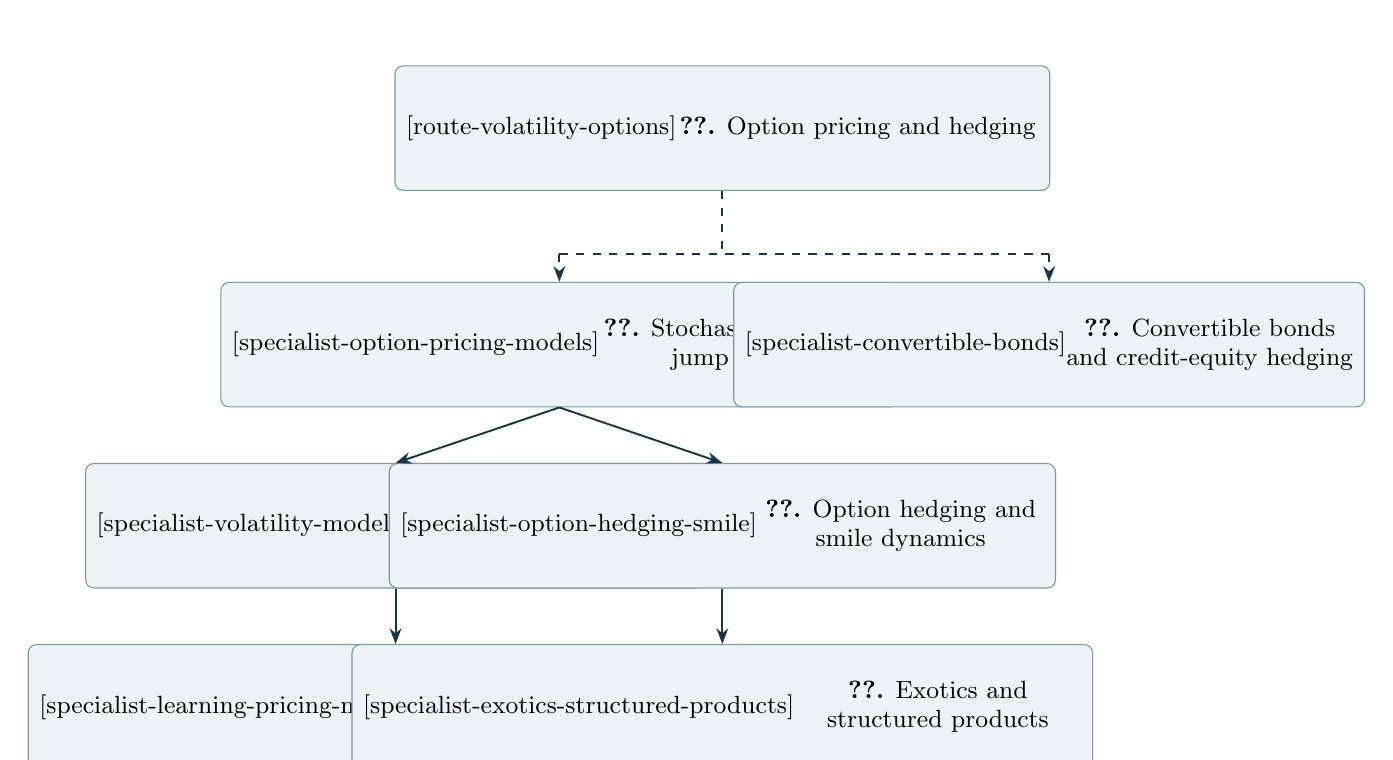
\begin{tikzpicture}[x=1cm,y=1cm]
\node[pathnode] (volatility-options) at (4.15,0) {\MeasurePathNode{4.6cm}{\textbf{\ref*{route-volatility-options}.} Option pricing and hedging}\hyperref[route-volatility-options]{\parbox[c][\pathnodeheight][c]{4.6cm}{\centering \textbf{\ref*{route-volatility-options}.} Option pricing and hedging}}};
\node[pathnode] (option-pricing-models) at (2.08,-2.75) {\MeasurePathNode{3.65cm}{\textbf{\ref*{specialist-option-pricing-models}.} Stochastic, local and jump models}\hyperref[specialist-option-pricing-models]{\parbox[c][\pathnodeheight][c]{3.65cm}{\centering \textbf{\ref*{specialist-option-pricing-models}.} Stochastic, local and jump models}}};
\node[pathnode] (convertible-bonds) at (8.30,-2.75) {\MeasurePathNode{3.65cm}{\textbf{\ref*{specialist-convertible-bonds}.} Convertible bonds and credit-equity hedging}\hyperref[specialist-convertible-bonds]{\parbox[c][\pathnodeheight][c]{3.65cm}{\centering \textbf{\ref*{specialist-convertible-bonds}.} Convertible bonds and credit-equity hedging}}};
\node[pathnode] (volatility-models) at (0.00,-5.05) {\MeasurePathNode{3.65cm}{\textbf{\ref*{specialist-volatility-models}.} Rough and path-dependent volatility}\hyperref[specialist-volatility-models]{\parbox[c][\pathnodeheight][c]{3.65cm}{\centering \textbf{\ref*{specialist-volatility-models}.} Rough and path-dependent volatility}}};
\node[pathnode] (option-hedging-smile) at (4.15,-5.05) {\MeasurePathNode{3.65cm}{\textbf{\ref*{specialist-option-hedging-smile}.} Option hedging and smile dynamics}\hyperref[specialist-option-hedging-smile]{\parbox[c][\pathnodeheight][c]{3.65cm}{\centering \textbf{\ref*{specialist-option-hedging-smile}.} Option hedging and smile dynamics}}};
\node[pathnode] (learning-pricing-model-risk) at (0.00,-7.35) {\MeasurePathNode{3.65cm}{\textbf{\ref*{specialist-learning-pricing-model-risk}.} Learned pricing and model risk}\hyperref[specialist-learning-pricing-model-risk]{\parbox[c][\pathnodeheight][c]{3.65cm}{\centering \textbf{\ref*{specialist-learning-pricing-model-risk}.} Learned pricing and model risk}}};
\node[pathnode] (exotics-structured-products) at (4.15,-7.35) {\MeasurePathNode{3.65cm}{\textbf{\ref*{specialist-exotics-structured-products}.} Exotics and structured products}\hyperref[specialist-exotics-structured-products]{\parbox[c][\pathnodeheight][c]{3.65cm}{\centering \textbf{\ref*{specialist-exotics-structured-products}.} Exotics and structured products}}};
\draw[entryline] (volatility-options.south) -- (4.15,-1.60);
\draw[entryline] (2.08,-1.60) -- (8.30,-1.60);
\draw[entryarrow] (2.08,-1.60) -- (option-pricing-models.north);
\draw[entryarrow] (8.30,-1.60) -- (convertible-bonds.north);
\draw[patharrow] (option-pricing-models.south) -- (volatility-models.north);
\draw[patharrow] (option-pricing-models.south) -- (option-hedging-smile.north);
\draw[patharrow] (volatility-models.south) -- (learning-pricing-model-risk.north);
\draw[patharrow] (option-hedging-smile.south) -- (exotics-structured-products.north);
\end{tikzpicture}\end{center}
\textbf{Bring these foundations with you.}\begin{itemize}
\item \hyperref[specialist-stochastic-calculus-control]{Stochastic calculus and continuous-time control} --- needed by \hyperref[specialist-option-pricing-models]{Stochastic, local and jump models}.
\item \hyperref[specialist-numerical-methods-optimisation]{Optimisation and numerical methods for pricing and portfolios} --- needed by \hyperref[specialist-learning-pricing-model-risk]{Learned pricing and model risk}.
\end{itemize}\hyperref[learning-map]{Return to the whole-guide DAG.}
\Needspace{12\baselineskip}
\subsection{Stochastic, local and jump volatility models}\label{specialist-option-pricing-models}
\textbf{Specialist pathway.} In \hyperref[route-volatility-options]{Option pricing, volatility models and hedging}.

\textbf{Outcome.} Calibrate local, stochastic and jump-diffusion models to the same surface, explain what each implies for smile dynamics and exotic prices, and test whether the fit survives out of sample.

\textbf{Prerequisites.} Option pricing, volatility models and hedging overview; stochastic calculus and Fourier or PDE pricing.

\textbf{Review first.} \hyperref[route-volatility-options]{Option pricing, volatility models and hedging}; \hyperref[specialist-stochastic-calculus-control]{Stochastic calculus and continuous-time control}.

\textbf{Required readings, in order}
\begin{enumerate}\raggedright
\Needspace{5\baselineskip}\item \href{institutional_quantitative_finance_reading_list.pdf\#s7-derman}{\emph{Emanuel Derman and Michael B. Miller, The Volatility Smile (2016)}}\CataloguePage{117}\NoteKey{s7-derman}\par \textbf{Mechanics.} Trace how local, stochastic and jump models each explain the smile, and what they imply for hedging and extrapolation.
\Needspace{5\baselineskip}\item \href{institutional_quantitative_finance_reading_list.pdf\#wide-merton-jumps}{Robert C. Merton, ``Option pricing when underlying stock returns are discontinuous''}\CataloguePage{118}\NoteKey{wide-merton-jumps}\par \textbf{Valuation.} Add jumps to the underlying and see why jump risk cannot be hedged with the stock alone.
\Needspace{5\baselineskip}\item \href{institutional_quantitative_finance_reading_list.pdf\#s6-heston}{Steven L. Heston, ``A Closed-Form Solution for Options with Stochastic Volatility with Applications to Bond and Currency Options''}\CataloguePage{118}\NoteKey{s6-heston}\par \textbf{Valuation.} Price under stochastic volatility with a closed-form characteristic function.
\Needspace{5\baselineskip}\item \href{institutional_quantitative_finance_reading_list.pdf\#wide-bates-svj}{David S. Bates, ``Jumps and Stochastic Volatility: Exchange Rate Processes Implicit in Deutsche Mark Options''}\CataloguePage{119}\NoteKey{wide-bates-svj}\par \textbf{Valuation.} Combine stochastic volatility with jumps, the standard SVJ extension, fitted to currency options.
\Needspace{5\baselineskip}\item \href{institutional_quantitative_finance_reading_list.pdf\#audit-duffie-pan-singleton}{Darrell Duffie, Jun Pan and Kenneth Singleton, ``Transform Analysis and Asset Pricing for Affine Jump-Diffusions''; author PDF}\CataloguePage{118}\NoteKey{audit-duffie-pan-singleton}\par \textbf{Theory.} Generalise to affine jump-diffusions through transform analysis.
\Needspace{5\baselineskip}\item \href{institutional_quantitative_finance_reading_list.pdf\#s6-carrmadan}{Peter Carr and Dilip Madan, ``Option Valuation Using the Fast Fourier Transform''}\CataloguePage{118}\NoteKey{s6-carrmadan}\par \textbf{Implementation.} Turn a characteristic function into prices across strikes with the fast Fourier transform.
\Needspace{5\baselineskip}\item \href{institutional_quantitative_finance_reading_list.pdf\#vo-lord-kahl-2010}{Roger Lord and Christian Kahl, ``Complex Logarithms in Heston-Like Models''}\CataloguePage{122}\NoteKey{vo-lord-kahl-2010}\par \textbf{Implementation.} Avoid branch-cut errors in Heston-type characteristic functions before trusting Fourier prices.
\Needspace{5\baselineskip}\item \href{institutional_quantitative_finance_reading_list.pdf\#wide-dupire-local-vol}{Bruno Dupire, ``Pricing with a Smile''}\CataloguePage{119}\NoteKey{wide-dupire-local-vol}\par \textbf{Valuation.} Back out the local-volatility function that reprices the whole call surface.
\Needspace{5\baselineskip}\item \href{institutional_quantitative_finance_reading_list.pdf\#wide-guyon-hl-nonlinear}{Julien Guyon and Pierre Henry-Labordère, \emph{Nonlinear Option Pricing}}\CataloguePage{125}\NoteKey{wide-guyon-hl-nonlinear}\par \textbf{Methods.} Calibrate local stochastic volatility to the surface with the particle method.
\Needspace{5\baselineskip}\item \href{institutional_quantitative_finance_reading_list.pdf\#vo-bakshi-cao-chen-1997}{Gurdip Bakshi, Charles Cao and Zhiwu Chen, ``Empirical Performance of Alternative Option Pricing Models''}\CataloguePage{119}\NoteKey{vo-bakshi-cao-chen-1997}\par \textbf{Evidence.} Compare stochastic-volatility, jump and stochastic-rate models on pricing, internal consistency and hedging.
\Needspace{5\baselineskip}\item \href{institutional_quantitative_finance_reading_list.pdf\#vo-dumas-fleming-whaley-1998}{Bernard Dumas, Jeff Fleming and Robert E. Whaley, ``Implied Volatility Functions: Empirical Tests''}\CataloguePage{119}\NoteKey{vo-dumas-fleming-whaley-1998}\par \textbf{Counter-evidence.} Test whether a deterministic local-volatility function beats smoothed Black--Scholes volatilities out of sample.
\Needspace{5\baselineskip}\item \href{institutional_quantitative_finance_reading_list.pdf\#vo-christoffersen-heston-jacobs-2009}{Peter Christoffersen, Steven Heston and Kris Jacobs, ``The Shape and Term Structure of the Index Option Smirk: Why Multifactor Stochastic Volatility Models Work So Well''}\CataloguePage{120}\NoteKey{vo-christoffersen-heston-jacobs-2009}\par \textbf{Evidence.} See why a second volatility factor is needed to move the smirk's level and slope independently.
\Needspace{5\baselineskip}\item \href{institutional_quantitative_finance_reading_list.pdf\#vo-schoutens-simons-tistaert-2004}{Wim Schoutens, Erwin Simons and Jurgen Tistaert, ``A Perfect Calibration! Now What?''}\CataloguePage{120}\NoteKey{vo-schoutens-simons-tistaert-2004}\par \textbf{Validation.} See models that fit the same vanillas give very different exotic prices.
\end{enumerate}
\Needspace{5\baselineskip}\textbf{Checkpoint.} On one day of SPX option quotes spanning at least three expiries, calibrate Dupire local volatility, Heston and Bates (or a two-factor model) using a stable characteristic function. Report fit by moneyness and maturity, recalibrate on the next five days to measure parameter stability, and price a down-and-out put and a forward-start call under each model; report the spread of exotic prices as model risk.

\textbf{Optional branches.} \href{institutional_quantitative_finance_reading_list.pdf\#wide-crr-binomial}{Price on a binomial tree and check its convergence to Black--Scholes.}\BranchPage{118} \href{institutional_quantitative_finance_reading_list.pdf\#wide-harrison-kreps}{Link the absence of arbitrage to equivalent martingale measures.}\BranchPage{118} \href{institutional_quantitative_finance_reading_list.pdf\#wide-harrison-pliska}{Formulate self-financing strategies and completeness in continuous time.}\BranchPage{118} \href{institutional_quantitative_finance_reading_list.pdf\#catalogue-0448}{Go deeper into Lévy and jump models, their calibration and hedging.}\BranchPage{116} \href{institutional_quantitative_finance_reading_list.pdf\#vo-kou-2002}{Use a double-exponential jump model with analytical path-dependent prices.}\BranchPage{119} \href{institutional_quantitative_finance_reading_list.pdf\#vo-carr-geman-madan-yor-2002}{Test whether index returns need a diffusion component at all.}\BranchPage{119} \href{institutional_quantitative_finance_reading_list.pdf\#vo-eraker-johannes-polson-2003}{Estimate jumps in both returns and volatility from index returns.}\BranchPage{120} \href{institutional_quantitative_finance_reading_list.pdf\#vo-broadie-chernov-johannes-2007}{Separate diffusive and jump risk premia in S\&P futures options.}\BranchPage{120} \href{institutional_quantitative_finance_reading_list.pdf\#vo-bates-2000}{See why stochastic volatility alone needs implausible parameters to match the post-1987 skew.}\BranchPage{119} \href{institutional_quantitative_finance_reading_list.pdf\#w3-letourneau-stentoft-panels}{Calibrate to large option panels, including early exercise.}\BranchPage{124} \href{institutional_quantitative_finance_reading_list.pdf\#w3-moussa-arbitrage-filter}{Filter quotes for static arbitrage in real time before calibrating.}\BranchPage{124} \href{institutional_quantitative_finance_reading_list.pdf\#wide-wilmott-pwoqf}{Read a PDE-centred practitioner treatment of derivatives modelling.}\BranchPage{117}
\par{\small \hyperref[learning-map]{Learning pathway DAG} \textbar{} \hyperref[route-volatility-options]{Section overview} \textbar{} \hyperref[map-volatility-options]{Section DAG}\NoteKey{option-pricing-models}}
\Needspace{12\baselineskip}
\subsection{Convertible bonds and credit-equity hedging}\label{specialist-convertible-bonds}
\textbf{Specialist pathway.} In \hyperref[route-volatility-options]{Option pricing, volatility models and hedging}.

\textbf{Outcome.} Combine default, equity optionality, conversion terms and stock-borrow economics.

\textbf{Prerequisites.} Option pricing, volatility models and hedging; bond cash flows, credit loss, discounting and option exercise.

\textbf{Review first.} \hyperref[route-volatility-options]{Option pricing, volatility models and hedging}.

\textbf{Required readings, in order}
\begin{enumerate}\raggedright
\Needspace{5\baselineskip}\item \href{institutional_quantitative_finance_reading_list.pdf\#gap-convertible-handbook}{Jan De Spiegeleer and Wim Schoutens, The Handbook of Convertible Bonds: Pricing, Strategies and Risk Management}\CataloguePage{142}\NoteKey{gap-convertible-handbook}\par \textbf{Market mechanics.} Map issuer credit, equity exposure, calls, puts and financing.
\Needspace{5\baselineskip}\item \href{institutional_quantitative_finance_reading_list.pdf\#gap-convertible-credit}{Elie Ayache, Peter A. Forsyth and Kenneth R. Vetzal, Valuation of Convertible Bonds With Credit Risk; Author manuscript}\CataloguePage{143}\NoteKey{gap-convertible-credit}\par \textbf{Numerical valuation.} Test default and stock-price consistency in the convertible pricing problem.
\Needspace{5\baselineskip}\item \href{institutional_quantitative_finance_reading_list.pdf\#remaining-convertible-contract}{The Southern Company, Second Supplemental Indenture: Series 2026B 3.50\% Convertible Senior Notes due 2029; issuance report}\CataloguePage{143}\NoteKey{remaining-convertible-contract}\par \textbf{Recent terms.} Translate conditional exercise and settlement into a contract state machine.
\Needspace{5\baselineskip}\item \href{institutional_quantitative_finance_reading_list.pdf\#al-davolio}{Gene D'Avolio, ``The Market for Borrowing Stock''}\CataloguePage{183}\NoteKey{al-davolio}\par \textbf{Hedge financing.} Include borrow availability, fees and recall in the equity hedge.
\Needspace{5\baselineskip}\item \href{institutional_quantitative_finance_reading_list.pdf\#w2-brennan-schwartz-convertible}{Michael J. Brennan and Eduardo S. Schwartz, ``Convertible Bonds: Valuation and Optimal Strategies for Call and Conversion''}\CataloguePage{143}\NoteKey{w2-brennan-schwartz-convertible}\par \textbf{Valuation.} Value convertibles with optimal call and conversion.
\Needspace{5\baselineskip}\item \href{institutional_quantitative_finance_reading_list.pdf\#w2-tsiveriotis-fernandes}{Kostas Tsiveriotis and Chris Fernandes, ``Valuing Convertible Bonds with Credit Risk''}\CataloguePage{143}\NoteKey{w2-tsiveriotis-fernandes}\par \textbf{Valuation.} Split cash and equity components with credit risk.
\Needspace{5\baselineskip}\item \href{institutional_quantitative_finance_reading_list.pdf\#w2-choi-convertible-supply}{Darwin Choi, Mila Getmansky, Brian Henderson and Heather Tookes, ``Convertible bond arbitrageurs as suppliers of capital''}\CataloguePage{143}\NoteKey{w2-choi-convertible-supply}\par \textbf{Evidence.} See convertible arbitrage funds supply issuer capital.
\Needspace{5\baselineskip}\item \href{institutional_quantitative_finance_reading_list.pdf\#w5-brown-grundy-convertibles}{Stephen J. Brown, Bruce D. Grundy, Craig M. Lewis and Patrick Verwijmeren, ``Convertibles and Hedge Funds as Distributors of Equity Exposure''}\CataloguePage{143}\NoteKey{w5-brown-grundy-convertibles}\par \textbf{Evidence.} See convertible arbitrageurs distribute issuers' equity exposure.
\end{enumerate}
\Needspace{5\baselineskip}\textbf{Checkpoint.} Implement a small hypothetical convertible benchmark with grid/time-step convergence and explicit default recovery. Separately build the Southern Series 2026B conversion-state and settlement ledger from its selected terms. Explain what the generic model omits before adapting it. Report equity delta, credit, rates, volatility and borrow-cost sensitivities; a calibrated hedge test additionally requires entitled quotes, dividends, borrow observations and transaction costs.

\textbf{Optional branches.} \href{institutional_quantitative_finance_reading_list.pdf\#wide-mitchell-pulvino-stafford-convert}{See convertible prices recover slowly after arbitrage capital leaves.}\BranchPage{143} \href{institutional_quantitative_finance_reading_list.pdf\#wide-agarwal-convertible-arb}{Build convertible-arbitrage risk factors from bond-level data.}\BranchPage{143} \href{institutional_quantitative_finance_reading_list.pdf\#w5-ammann-kind-wilde}{Compare market prices of French convertibles with model values.}\BranchPage{144}
\par{\small \hyperref[learning-map]{Learning pathway DAG} \textbar{} \hyperref[route-volatility-options]{Section overview} \textbar{} \hyperref[map-volatility-options]{Section DAG}\NoteKey{convertible-bonds}}
\Needspace{12\baselineskip}
\subsection{Rough and path-dependent volatility}\label{specialist-volatility-models}
\textbf{Specialist pathway.} In \hyperref[route-volatility-options]{Option pricing, volatility models and hedging}.

\textbf{Outcome.} Compare rough, path-dependent and Markovian volatility specifications on matched quotes and hedge tests.

\textbf{Prerequisites.} Stochastic, local and jump volatility models; stochastic calculus, numerical pricing and option Greeks.

\textbf{Review first.} \hyperref[specialist-option-pricing-models]{Stochastic, local and jump volatility models}.

\textbf{Required readings, in order}
\begin{enumerate}\raggedright
\Needspace{5\baselineskip}\item \href{institutional_quantitative_finance_reading_list.pdf\#s6-rough}{Jim Gatheral, Thibault Jaisson and Mathieu Rosenbaum, ``Volatility Is Rough''}\CataloguePage{120}\NoteKey{s6-rough}\par \textbf{Evidence.} Understand the original high-frequency rough-volatility finding.
\Needspace{5\baselineskip}\item \href{institutional_quantitative_finance_reading_list.pdf\#add-pdv}{Julien Guyon and Jordan Lekeufack, Volatility Is (Mostly) Path-Dependent}\CataloguePage{120}\NoteKey{add-pdv}\par \textbf{Valuation.} Build a competing path-dependent volatility mechanism.
\Needspace{5\baselineskip}\item \href{institutional_quantitative_finance_reading_list.pdf\#s7-bergomi}{Lorenzo Bergomi, \emph{Stochastic Volatility Modeling}}\CataloguePage{116}\NoteKey{s7-bergomi}\par \textbf{Valuation.} Relate forward variance, smile dynamics and hedging assumptions.
\Needspace{5\baselineskip}\item \href{institutional_quantitative_finance_reading_list.pdf\#exp-bayer-friz-gatheral-rbergomi}{Christian Bayer; Peter Friz; Jim Gatheral, Pricing under rough volatility; publisher erratum}\CataloguePage{123}\NoteKey{exp-bayer-friz-gatheral-rbergomi}\par \textbf{Valuation.} Price a concrete rough-volatility specification.
\Needspace{5\baselineskip}\item \href{institutional_quantitative_finance_reading_list.pdf\#add-vol-comparison}{Eduardo Abi Jaber and Shaun (Xiaoyuan) Li, Volatility Models in Practice: Rough, Path-Dependent, or Markovian?}\CataloguePage{120}\NoteKey{add-vol-comparison}\par \textbf{Evidence.} Use a recent matched-parameter comparison to challenge model choice.
\Needspace{5\baselineskip}\item \href{institutional_quantitative_finance_reading_list.pdf\#exp-gatheral-jacquier-svi}{Jim Gatheral; Antoine Jacquier, Arbitrage-free SVI volatility surfaces}\CataloguePage{123}\NoteKey{exp-gatheral-jacquier-svi}\par \textbf{Mechanics.} Establish static-arbitrage checks for the observed surface.
\Needspace{5\baselineskip}\item \href{institutional_quantitative_finance_reading_list.pdf\#gap-cboe-vix6}{Cboe Global Indices, Cboe Volatility Index Methodology}\CataloguePage{135}\NoteKey{gap-cboe-vix6}\par \textbf{Data.} Reproduce VIX input and maturity conventions from the current methodology.
\Needspace{5\baselineskip}\item \href{institutional_quantitative_finance_reading_list.pdf\#gapclose-cboe-spx-quote-data}{Cboe DataShop, Option Quote Intervals; Option EOD Summary; data conventions FAQ}\CataloguePage{116}\NoteKey{gapclose-cboe-spx-quote-data}\par \textbf{Quote data.} Obtain timestamped SPX option NBBO snapshots and license-matched underlying values for empirical calibration.
\Needspace{5\baselineskip}\item \href{institutional_quantitative_finance_reading_list.pdf\#exp-mccrickerd-pakkanen-rbergomi-mc}{Ryan McCrickerd; Mikko S. Pakkanen, Turbocharging Monte Carlo pricing for the rough Bergomi model; author preprint}\CataloguePage{123}\NoteKey{exp-mccrickerd-pakkanen-rbergomi-mc}\par \textbf{Implementation.} Control simulation error and runtime in calibration.
\Needspace{5\baselineskip}\item \href{institutional_quantitative_finance_reading_list.pdf\#exp-bayer-breneis-rough-heston-scheme}{Christian Bayer; Simon Breneis, Efficient option pricing in the rough Heston model using weak simulation schemes; author manuscript}\CataloguePage{124}\NoteKey{exp-bayer-breneis-rough-heston-scheme}\par \textbf{Implementation.} Assess low-dimensional weak simulation as a pricing alternative.
\Needspace{5\baselineskip}\item \href{institutional_quantitative_finance_reading_list.pdf\#exp-cont-vuletic-generative-hedging}{Rama Cont; Milena Vuletić, Data-driven hedging with generative models; Oxford version of record}\CataloguePage{128}\NoteKey{exp-cont-vuletic-generative-hedging}\par \textbf{Implementation.} Evaluate out-of-sample hedge consequences separately from smile fit.
\end{enumerate}
\Needspace{5\baselineskip}\textbf{Checkpoint.} Specify a timestamped SPX option sample using the Cboe interval/EOD fields and obtain separately entitled matching underlying values. Filter stale, zero and crossed quotes, distinguish AM/PM settlement and preserve the quote-size convention vintage. Calibrate SVI and rough, path-dependent and Markovian models with matched parameter budgets, reporting fit, arbitrage and runtime. Future hedge tests require subsequent tradable observations. If licensed inputs are unavailable, use a labelled synthetic exercise and omit empirical-performance claims.

\textbf{Optional branches.} \href{institutional_quantitative_finance_reading_list.pdf\#wide-cont-das-rough}{Check whether measured roughness is an estimation artefact.}\BranchPage{125} \href{institutional_quantitative_finance_reading_list.pdf\#wide-gatheral-quadratic-rough-heston}{Fit SPX and VIX smiles jointly.}\BranchPage{125} \href{institutional_quantitative_finance_reading_list.pdf\#w4-zaugg-grzelak-lifted-heston}{Simulate the lifted Heston model with large steps.}\BranchPage{123} \href{institutional_quantitative_finance_reading_list.pdf\#w4-han-schied-hurst}{Estimate roughness (Hurst) consistently.}\BranchPage{121} \href{institutional_quantitative_finance_reading_list.pdf\#catalogue-0450}{Price rough Heston through its fractional Riccati characteristic function.}\BranchPage{121} \href{institutional_quantitative_finance_reading_list.pdf\#catalogue-0451}{Consult the edited rough-volatility volume before using rough models in production.}\BranchPage{121} \href{institutional_quantitative_finance_reading_list.pdf\#catalogue-0452}{Try signature volatility models priced with Fourier methods.}\BranchPage{121} \href{institutional_quantitative_finance_reading_list.pdf\#w3-andres-iv-path-dependent}{Simulate the implied-volatility surface jointly with path-dependent volatility.}\BranchPage{121} \href{institutional_quantitative_finance_reading_list.pdf\#w3-dugo-multivariate-rough}{Extend rough volatility to several assets.}\BranchPage{121}
\par{\small \hyperref[learning-map]{Learning pathway DAG} \textbar{} \hyperref[route-volatility-options]{Section overview} \textbar{} \hyperref[map-volatility-options]{Section DAG}\NoteKey{volatility-models}}
\Needspace{12\baselineskip}
\subsection{Option hedging: delta, vega, smile dynamics and transaction costs}\label{specialist-option-hedging-smile}
\textbf{Specialist pathway.} In \hyperref[route-volatility-options]{Option pricing, volatility models and hedging}.

\textbf{Outcome.} Choose and test delta and vega hedges under smile dynamics, discrete rebalancing and transaction costs, and attribute option profit and loss to its gamma, vega and residual sources.

\textbf{Prerequisites.} Stochastic, local and jump volatility models; option Greeks and simulation.

\textbf{Review first.} \hyperref[specialist-option-pricing-models]{Stochastic, local and jump volatility models}.

\textbf{Required readings, in order}
\begin{enumerate}\raggedright
\Needspace{5\baselineskip}\item \href{institutional_quantitative_finance_reading_list.pdf\#s7-natenberg}{Sheldon Natenberg, \emph{Option Volatility \& Pricing: Advanced Trading Strategies and Techniques}, 2nd ed. (published 2014; copyright 2015)}\CataloguePage{117}\NoteKey{s7-natenberg}\par \textbf{Mechanics.} Learn the Greeks, spreads and position risks as an option market maker manages them.
\Needspace{5\baselineskip}\item \href{institutional_quantitative_finance_reading_list.pdf\#s7-taleb}{\emph{Nassim Nicholas Taleb, Dynamic Hedging (1997)}}\CataloguePage{117}\NoteKey{s7-taleb}\par \textbf{Mechanics.} Rehedge option books when smiles shift, liquidity thins and prices gap.
\Needspace{5\baselineskip}\item \href{institutional_quantitative_finance_reading_list.pdf\#vo-el-karoui-jeanblanc-shreve-1998}{Nicole El Karoui, Monique Jeanblanc-Picqué and Steven E. Shreve, ``Robustness of the Black and Scholes Formula''}\CataloguePage{126}\NoteKey{vo-el-karoui-jeanblanc-shreve-1998}\par \textbf{Theory.} See why a hedge at an overstated volatility super-replicates, and when that robustness fails.
\Needspace{5\baselineskip}\item \href{institutional_quantitative_finance_reading_list.pdf\#vo-carr-wu-2020}{Peter Carr and Liuren Wu, ``Option Profit and Loss Attribution and Pricing: A New Framework''}\CataloguePage{126}\NoteKey{vo-carr-wu-2020}\par \textbf{Theory.} Attribute daily option profit and loss to moves in the underlying and in implied volatility, and price from that attribution.
\Needspace{5\baselineskip}\item \href{institutional_quantitative_finance_reading_list.pdf\#vo-figlewski-1989}{Stephen Figlewski, ``Options Arbitrage in Imperfect Markets''}\CataloguePage{126}\NoteKey{vo-figlewski-1989}\par \textbf{Evidence.} Measure how discrete rebalancing, uncertain volatility and costs widen the bounds that arbitrage sets.
\Needspace{5\baselineskip}\item \href{institutional_quantitative_finance_reading_list.pdf\#vo-leland-1985}{Hayne E. Leland, ``Option Pricing and Replication with Transactions Costs''}\CataloguePage{126}\NoteKey{vo-leland-1985}\par \textbf{Theory.} Adjust the hedging volatility so that replication covers transaction costs.
\Needspace{5\baselineskip}\item \href{institutional_quantitative_finance_reading_list.pdf\#vo-whalley-wilmott-1997}{A. Elizabeth Whalley and Paul Wilmott, ``An Asymptotic Analysis of an Optimal Hedging Model for Option Pricing with Transaction Costs''}\CataloguePage{126}\NoteKey{vo-whalley-wilmott-1997}\par \textbf{Implementation.} Use the asymptotic no-trade band around delta as a practical rebalancing rule.
\Needspace{5\baselineskip}\item \href{institutional_quantitative_finance_reading_list.pdf\#wide-hagan-sabr}{Patrick S. Hagan, Deep Kumar, Andrew S. Lesniewski and Diana E. Woodward, ``Managing Smile Risk''}\CataloguePage{119}\NoteKey{wide-hagan-sabr}\par \textbf{Valuation.} See why local volatility predicts the wrong smile dynamics and how SABR changes the hedge.
\Needspace{5\baselineskip}\item \href{institutional_quantitative_finance_reading_list.pdf\#vo-crepey-2004}{Stéphane Crépey, ``Delta-Hedging Vega Risk?''}\CataloguePage{127}\NoteKey{vo-crepey-2004}\par \textbf{Evidence.} Compare local-volatility and Black--Scholes implied deltas in skewed markets.
\Needspace{5\baselineskip}\item \href{institutional_quantitative_finance_reading_list.pdf\#vo-hull-white-2017}{John Hull and Alan White, ``Optimal Delta Hedging for Options''}\CataloguePage{127}\NoteKey{vo-hull-white-2017}\par \textbf{Evidence.} Estimate the minimum-variance delta that allows for the expected volatility move.
\Needspace{5\baselineskip}\item \href{institutional_quantitative_finance_reading_list.pdf\#exp-cont-vuletic-generative-hedging}{Rama Cont; Milena Vuletić, Data-driven hedging with generative models; Oxford version of record}\CataloguePage{128}\NoteKey{exp-cont-vuletic-generative-hedging}\par \textbf{Implementation.} Compare data-driven scenario hedges with delta and delta-vega baselines, including model-risk limits.
\end{enumerate}
\Needspace{5\baselineskip}\textbf{Checkpoint.} Backtest daily hedging of a three-month SPX put over at least two years using Black--Scholes delta at implied and at forecast volatility, a sticky-strike delta against a SABR or local-volatility delta, and the minimum-variance delta, each with and without a vega hedge. Add a Whalley--Wilmott no-trade band with measured spreads. Attribute daily profit and loss to gamma--theta, vega and residual terms and report the mean, dispersion and tails of hedging error net of costs.

\textbf{Optional branches.} \href{institutional_quantitative_finance_reading_list.pdf\#vo-alexander-nogueira-2007}{Use model-free hedge ratios and see when they are not minimum-variance.}\BranchPage{127} \href{institutional_quantitative_finance_reading_list.pdf\#catalogue-0455}{Check whether learned hedges beat delta hedging on real intraday option data.}\BranchPage{127} \href{institutional_quantitative_finance_reading_list.pdf\#wide-giles-glasserman-adjoints}{Compute Monte Carlo Greeks quickly by adjoint differentiation.}\BranchPage{122} \href{institutional_quantitative_finance_reading_list.pdf\#w4-armstrong-gamma-rough}{Gamma-hedge when price paths are rough.}\BranchPage{129} \href{institutional_quantitative_finance_reading_list.pdf\#w2-rebonato-volcorr}{Read a modeller's account of smile dynamics and correlation hedging.}\BranchPage{139} \href{institutional_quantitative_finance_reading_list.pdf\#w5-sinclair-option-trading}{Choose hedging rules and trade sizes when buying or selling volatility.}\BranchPage{140} \href{institutional_quantitative_finance_reading_list.pdf\#s7-mcmillan}{Use a reference of option strategies and payoff diagrams for scenario analysis.}\BranchPage{117}
\par{\small \hyperref[learning-map]{Learning pathway DAG} \textbar{} \hyperref[route-volatility-options]{Section overview} \textbar{} \hyperref[map-volatility-options]{Section DAG}\NoteKey{option-hedging-smile}}
\Needspace{12\baselineskip}
\subsection{Learning-based pricing, calibration and model risk}\label{specialist-learning-pricing-model-risk}
\textbf{Specialist pathway.} In \hyperref[route-volatility-options]{Option pricing, volatility models and hedging}.

\textbf{Outcome.} Use neural approximators and deep solvers for pricing and calibration while quantifying model risk with robust bounds.

\textbf{Prerequisites.} Rough and path-dependent volatility; numerical methods and ML basics.

\textbf{Review first.} \hyperref[specialist-volatility-models]{Rough and path-dependent volatility}; \hyperref[specialist-numerical-methods-optimisation]{Optimisation and numerical methods for pricing and portfolios}.

\textbf{Required readings, in order}
\begin{enumerate}\raggedright
\Needspace{5\baselineskip}\item \href{institutional_quantitative_finance_reading_list.pdf\#wide-hutchinson-lo-poggio}{James M. Hutchinson, Andrew W. Lo and Tomaso Poggio, ``A Nonparametric Approach to Pricing and Hedging Derivative Securities Via Learning Networks''}\CataloguePage{128}\NoteKey{wide-hutchinson-lo-poggio}\par \textbf{Foundations.} See the original learning-network pricing idea.
\Needspace{5\baselineskip}\item \href{institutional_quantitative_finance_reading_list.pdf\#wide-ruf-wang-review}{Johannes Ruf and Weiguan Wang, ``Neural networks for option pricing and hedging: a literature review''}\CataloguePage{128}\NoteKey{wide-ruf-wang-review}\par \textbf{Validation.} Avoid leakage and weak benchmarks in neural pricing.
\Needspace{5\baselineskip}\item \href{institutional_quantitative_finance_reading_list.pdf\#wide-horvath-dl-vol}{Blanka Horvath, Aitor Muguruza and Mehdi Tomas, ``Deep learning volatility: a deep neural network perspective on pricing and calibration in (rough) volatility models''}\CataloguePage{125}\NoteKey{wide-horvath-dl-vol}\par \textbf{Methods.} Calibrate rough models through a learned pricing map.
\Needspace{5\baselineskip}\item \href{institutional_quantitative_finance_reading_list.pdf\#wide-huge-savine-dml}{Brian Huge and Antoine Savine, ``Differential Machine Learning''}\CataloguePage{122}\NoteKey{wide-huge-savine-dml}\par \textbf{Methods.} Train with differential labels for accurate Greeks.
\Needspace{5\baselineskip}\item \href{institutional_quantitative_finance_reading_list.pdf\#wide-becker-deep-stopping}{Sebastian Becker, Patrick Cheridito and Arnulf Jentzen, ``Deep Optimal Stopping''}\CataloguePage{129}\NoteKey{wide-becker-deep-stopping}\par \textbf{Valuation.} Price high-dimensional Bermudans with bounds.
\Needspace{5\baselineskip}\item \href{institutional_quantitative_finance_reading_list.pdf\#wide-han-jentzen-e}{Jiequn Han, Arnulf Jentzen and Weinan E, ``Solving high-dimensional partial differential equations using deep learning''}\CataloguePage{129}\NoteKey{wide-han-jentzen-e}\par \textbf{Methods.} Solve high-dimensional PDEs with deep BSDEs.
\Needspace{5\baselineskip}\item \href{institutional_quantitative_finance_reading_list.pdf\#catalogue-0453}{Hans Buehler, Lukas Gonon, Josef Teichmann and Ben Wood, ``Deep Hedging''}\CataloguePage{127}\NoteKey{catalogue-0453}\par \textbf{Implementation.} Learn hedging strategies with costs directly.
\Needspace{5\baselineskip}\item \href{institutional_quantitative_finance_reading_list.pdf\#wide-cont-model-uncertainty}{Rama Cont, ``Model uncertainty and its impact on the pricing of derivative instruments''}\CataloguePage{124}\NoteKey{wide-cont-model-uncertainty}\par \textbf{Validation.} Measure model risk across calibrated models.
\Needspace{5\baselineskip}\item \href{institutional_quantitative_finance_reading_list.pdf\#wide-beiglbock-mot}{Mathias Beiglböck, Pierre Henry-Labordère and Friedrich Penkner, ``Model-independent bounds for option prices---a mass transport approach''}\CataloguePage{125}\NoteKey{wide-beiglbock-mot}\par \textbf{Theory.} Derive model-independent bounds from vanillas.
\Needspace{5\baselineskip}\item \href{institutional_quantitative_finance_reading_list.pdf\#wide-cont-das-rough}{Rama Cont and Purba Das, ``Rough Volatility: Fact or Artefact?''}\CataloguePage{125}\NoteKey{wide-cont-das-rough}\par \textbf{Counter-evidence.} Question whether volatility is really rough.
\Needspace{5\baselineskip}\item \href{institutional_quantitative_finance_reading_list.pdf\#wide-guyon-spx-vix}{Julien Guyon, ``The Joint S\&P 500/VIX Smile Calibration Puzzle Solved''}\CataloguePage{125}\NoteKey{wide-guyon-spx-vix}\par \textbf{Evidence.} Study joint SPX/VIX calibration.
\end{enumerate}
\Needspace{5\baselineskip}\textbf{Checkpoint.} Train a neural surrogate of a rough or Heston pricer, calibrate to one day of SPX options, and compare with direct calibration on speed and error; compute model-free bounds for a forward-start option and report how far calibrated model prices fall within them.

\textbf{Optional branches.} \href{institutional_quantitative_finance_reading_list.pdf\#wide-henry-labordere-mfh}{Go deeper into martingale optimal transport.}\BranchPage{125} \href{institutional_quantitative_finance_reading_list.pdf\#wide-green-dl-quant-finance}{Read a practitioner deep-learning text for pricing.}\BranchPage{52} \href{institutional_quantitative_finance_reading_list.pdf\#w3-li-phillips-long-memory}{Weigh long memory against roughness.}\BranchPage{38} \href{institutional_quantitative_finance_reading_list.pdf\#w3-chen-model-free-gaps}{Measure empirical model-free hedging gaps.}\BranchPage{125} \href{institutional_quantitative_finance_reading_list.pdf\#w3-fan-sirignano-ml-derivatives}{Calibrate neural SDEs to derivative prices.}\BranchPage{129} \href{institutional_quantitative_finance_reading_list.pdf\#w4-guyon-schrodinger-spx-vix}{Jointly calibrate SPX and VIX smiles by minimum entropy.}\BranchPage{126} \href{institutional_quantitative_finance_reading_list.pdf\#exp-baschetti-random-grid-calibration}{Train neural calibration maps on random strike--maturity grids.}\BranchPage{124} \href{institutional_quantitative_finance_reading_list.pdf\#w3-chen-didisheim-surrogates}{Replace slow structural pricers with deep surrogates.}\BranchPage{129} \href{institutional_quantitative_finance_reading_list.pdf\#w4-cuchiero-bayesian-neural-sde}{Calibrate neural SDE models robustly with Bayesian methods.}\BranchPage{124} \href{institutional_quantitative_finance_reading_list.pdf\#exp-vuletic-cont-volgan}{Generate arbitrage-free implied-volatility surface scenarios.}\BranchPage{124} \href{institutional_quantitative_finance_reading_list.pdf\#catalogue-0800}{Train hedges that stay robust when the simulator is misspecified.}\BranchPage{127} \href{institutional_quantitative_finance_reading_list.pdf\#catalogue-0454}{Learn hedges from historical market transitions with an actor--critic method.}\BranchPage{127} \href{institutional_quantitative_finance_reading_list.pdf\#catalogue-0804}{Optimise tail-risk hedges on crisis-era simulators with explicit frictions.}\BranchPage{128} \href{institutional_quantitative_finance_reading_list.pdf\#wide-sirignano-dgm}{Solve high-dimensional pricing PDEs with the deep Galerkin method.}\BranchPage{129}
\par{\small \hyperref[learning-map]{Learning pathway DAG} \textbar{} \hyperref[route-volatility-options]{Section overview} \textbar{} \hyperref[map-volatility-options]{Section DAG}\NoteKey{learning-pricing-model-risk}}
\Needspace{12\baselineskip}
\subsection{Exotic options, autocallables and structured products}\label{specialist-exotics-structured-products}
\textbf{Specialist pathway.} In \hyperref[route-volatility-options]{Option pricing, volatility models and hedging}.

\textbf{Outcome.} Price and statically hedge barrier and other path-dependent payoffs, value autocallables, measure the margins in retail structured products, and trace issuers' hedging into the volatility surface.

\textbf{Prerequisites.} Option hedging; stochastic, local and jump volatility models; Monte Carlo and PDE pricing.

\textbf{Review first.} \hyperref[specialist-option-hedging-smile]{Option hedging: delta, vega, smile dynamics and transaction costs}.

\textbf{Required readings, in order}
\begin{enumerate}\raggedright
\Needspace{5\baselineskip}\item \href{institutional_quantitative_finance_reading_list.pdf\#wide-bouzoubaa-osseiran}{Mohamed Bouzoubaa and Adel Osseiran, \emph{Exotic Options and Hybrids: A Guide to Structuring, Pricing and Trading}}\CataloguePage{144}\NoteKey{wide-bouzoubaa-osseiran}\par \textbf{Mechanics.} Map barrier, cliquet, autocallable, basket and hybrid payoffs to the risks a structuring desk carries.
\Needspace{5\baselineskip}\item \href{institutional_quantitative_finance_reading_list.pdf\#vo-broadie-glasserman-kou-1997}{Mark Broadie, Paul Glasserman and Steven Kou, ``A Continuity Correction for Discrete Barrier Options''}\CataloguePage{144}\NoteKey{vo-broadie-glasserman-kou-1997}\par \textbf{Valuation.} Price discretely monitored barriers with the continuity correction.
\Needspace{5\baselineskip}\item \href{institutional_quantitative_finance_reading_list.pdf\#vo-derman-ergener-kani-1995}{Emanuel Derman, Deniz Ergener and Iraj Kani, ``Static Options Replication''}\CataloguePage{144}\NoteKey{vo-derman-ergener-kani-1995}\par \textbf{Implementation.} Replicate an exotic with a fixed portfolio of standard options.
\Needspace{5\baselineskip}\item \href{institutional_quantitative_finance_reading_list.pdf\#vo-carr-ellis-gupta-1998}{Peter Carr, Katrina Ellis and Vishal Gupta, ``Static Hedging of Exotic Options''}\CataloguePage{144}\NoteKey{vo-carr-ellis-gupta-1998}\par \textbf{Methods.} Build static hedges for exotics from puts and calls at other strikes, including under a smile.
\Needspace{5\baselineskip}\item \href{institutional_quantitative_finance_reading_list.pdf\#vo-guillaume-2015}{Tristan Guillaume, ``Autocallable Structured Products''}\CataloguePage{144}\NoteKey{vo-guillaume-2015}\par \textbf{Valuation.} Value autocallables with memory coupons, knock-in puts and worst-of features.
\Needspace{5\baselineskip}\item \href{institutional_quantitative_finance_reading_list.pdf\#gap-autocall-ctmc}{Yeda Cui, Lingfei Li and Gongqiu Zhang, Pricing and hedging autocallable products by Markov chain approximation}\CataloguePage{144}\NoteKey{gap-autocall-ctmc}\par \textbf{Implementation.} Price and hedge autocallables by Markov-chain approximation and compare with Monte Carlo.
\Needspace{5\baselineskip}\item \href{institutional_quantitative_finance_reading_list.pdf\#vo-yoon-2014}{Sun-Joong Yoon, ``Structured Products Markets and Implied Volatility Distortion''}\CataloguePage{145}\NoteKey{vo-yoon-2014}\par \textbf{Evidence.} See how issuers hedging step-down autocallables push down Korean implied volatility.
\Needspace{5\baselineskip}\item \href{institutional_quantitative_finance_reading_list.pdf\#vo-wallmeier-diethelm-2009}{Martin Wallmeier and Martin Diethelm, ``Market Pricing of Exotic Structured Products: The Case of Multi-Asset Barrier Reverse Convertibles in Switzerland''}\CataloguePage{145}\NoteKey{vo-wallmeier-diethelm-2009}\par \textbf{Evidence.} Measure the premium Swiss investors pay for multi-asset barrier reverse convertibles.
\Needspace{5\baselineskip}\item \href{institutional_quantitative_finance_reading_list.pdf\#w5-henderson-pearson-dark-side}{Brian J. Henderson and Neil D. Pearson, ``The dark side of financial innovation: A case study of the pricing of a retail financial product''}\CataloguePage{145}\NoteKey{w5-henderson-pearson-dark-side}\par \textbf{Evidence.} Measure the overpricing of a popular retail structured note.
\Needspace{5\baselineskip}\item \href{institutional_quantitative_finance_reading_list.pdf\#w5-celerier-vallee}{Claire Célérier and Boris Vallée, ``Catering to Investors Through Security Design: Headline Rate and Complexity''}\CataloguePage{145}\NoteKey{w5-celerier-vallee}\par \textbf{Evidence.} See product complexity used to cater to yield-seeking households.
\Needspace{5\baselineskip}\item \href{institutional_quantitative_finance_reading_list.pdf\#vo-egan-2019}{Mark Egan, ``Brokers versus Retail Investors: Conflicting Interests and Dominated Products''}\CataloguePage{145}\NoteKey{vo-egan-2019}\par \textbf{Evidence.} See brokers steer clients to dominated retail convertibles that pay higher fees.
\Needspace{5\baselineskip}\item \href{institutional_quantitative_finance_reading_list.pdf\#w5-vokata-lemons}{Petra Vokata, ``Engineering lemons''}\CataloguePage{145}\NoteKey{w5-vokata-lemons}\par \textbf{Evidence.} Measure the returns investors earn on yield-enhancing products.
\Needspace{5\baselineskip}\item \href{institutional_quantitative_finance_reading_list.pdf\#w4-asness-buffer-funds}{Cliff Asness, Jeffrey Cao, Antti Ilmanen and Dan Villalon, ``Rebuffed: An Empirical Review of Buffer Funds''}\CataloguePage{145}\NoteKey{w4-asness-buffer-funds}\par \textbf{Evidence.} Test whether buffer (defined-outcome) funds beat simple stock--cash mixes.
\end{enumerate}
\Needspace{5\baselineskip}\textbf{Checkpoint.} Price a three-year worst-of autocallable on two equity indices, with a down-and-in put, memory coupons and quarterly observation, under local volatility and under Heston or local stochastic volatility, by Monte Carlo with the barrier correction where it applies. Report the vega and correlation exposure left with the issuer, a partial static hedge from listed options, and the issue margin implied by a comparable term sheet's price; state which terms come from a real prospectus and which are assumed.

\textbf{Optional branches.} \href{institutional_quantitative_finance_reading_list.pdf\#catalogue-0457}{Read a desk-level treatment of equity hybrid products and their models.}\BranchPage{116} \href{institutional_quantitative_finance_reading_list.pdf\#vo-bernard-boyle-gornall-2011}{See locally capped retail products overpriced by about 6.5\%.}\BranchPage{145} \href{institutional_quantitative_finance_reading_list.pdf\#vo-schoutens-simons-tistaert-2004}{Recheck exotic prices across models that fit the same vanillas.}\BranchPage{120}
\par{\small \hyperref[learning-map]{Learning pathway DAG} \textbar{} \hyperref[route-volatility-options]{Section overview} \textbar{} \hyperref[map-volatility-options]{Section DAG}\NoteKey{exotics-structured-products}}
\clearpage
\section{Volatility trading, option premia and implied information}\label{route-volatility-trading-premia}
\label{route-25}
\textbf{Learning sequence.} Start with index option returns, variance premia and dealer hedging and with option-implied densities and tail risk; continue to single-stock option returns, VIX, correlation and dividend claims, and short-dated and retail option trading. Options market making is in Part III.

\textbf{Section goals.} Across its pathways, this section teaches you to:
\begin{itemize}[leftmargin=1.4em,itemsep=0pt,topsep=1pt]
\item replicate variance claims, measure variance and skew premia, and trace dealer gamma hedging (\hyperref[specialist-option-premia-dealers]{\ref*{specialist-option-premia-dealers}})
\item extract risk-neutral densities, tail measures and jump premia and test what they forecast (\hyperref[specialist-option-implied-information]{\ref*{specialist-option-implied-information}})
\item explain single-stock option returns with volatility, characteristics and option factors (\hyperref[specialist-equity-option-returns]{\ref*{specialist-equity-option-returns}})
\item price and hedge VIX, correlation, dispersion and dividend claims (\hyperref[specialist-vix-correlation-dividends]{\ref*{specialist-vix-correlation-dividends}})
\item price short-dated options and measure what retail option traders pay (\hyperref[specialist-short-dated-retail-options]{\ref*{specialist-short-dated-retail-options}})
\end{itemize}
\textbf{Overview outcome.} Measure the variance risk premium and risk-neutral volatility and skewness in index and single-stock options, and test how much of the premium survives crash months, quoted spreads and margin.

\textbf{Prerequisites.} Option pricing, volatility models and hedging; time-series volatility forecasting.

\textbf{Review first.} \hyperref[route-volatility-options]{Option pricing, volatility models and hedging}; \hyperref[specialist-time-series-volatility]{Time-series econometrics and volatility forecasting}.

\textbf{Required readings, in order}
\begin{enumerate}\raggedright
\Needspace{5\baselineskip}\item \href{institutional_quantitative_finance_reading_list.pdf\#alpha-sinclair}{Euan Sinclair, \emph{Volatility Trading}, 2nd ed. (2013)}\CataloguePage{139}\NoteKey{alpha-sinclair}\par See how a practitioner forecasts volatility, judges implied against realised volatility and sizes option trades.
\Needspace{5\baselineskip}\item \href{institutional_quantitative_finance_reading_list.pdf\#gap-carr-wu-variance}{Peter Carr and Liuren Wu, Variance Risk Premiums}\CataloguePage{130}\NoteKey{gap-carr-wu-variance}\par Distinguish priced variance exposure from a model's volatility forecast.
\Needspace{5\baselineskip}\item \href{institutional_quantitative_finance_reading_list.pdf\#wide-bakshi-kapadia-madan}{Gurdip Bakshi, Nikunj Kapadia and Dilip Madan, ``Stock Return Characteristics, Skew Laws, and the Differential Pricing of Individual Equity Options''}\CataloguePage{131}\NoteKey{wide-bakshi-kapadia-madan}\par Compute model-free risk-neutral volatility, skewness and kurtosis from a strip of options.
\Needspace{5\baselineskip}\item \href{institutional_quantitative_finance_reading_list.pdf\#s7-bondarenko}{\emph{Oleg Bondarenko, ``Why Are Put Options So Expensive?'' (2014)}}\CataloguePage{130}\NoteKey{s7-bondarenko}\par Weigh why index puts have earned such negative returns and which explanations fall short.
\Needspace{5\baselineskip}\item \href{institutional_quantitative_finance_reading_list.pdf\#vo-constantinides-jackwerth-savov-2013}{George M. Constantinides, Jens Carsten Jackwerth and Alexi Savov, ``The Puzzle of Index Option Returns''}\CataloguePage{130}\NoteKey{vo-constantinides-jackwerth-savov-2013}\par Price index option portfolios with a crisis factor before calling put returns an anomaly.
\Needspace{5\baselineskip}\item \href{institutional_quantitative_finance_reading_list.pdf\#w2-ilmanen-insurance}{Antti Ilmanen, ``Do Financial Markets Reward Buying or Selling Insurance and Lottery Tickets?''}\CataloguePage{105}\NoteKey{w2-ilmanen-insurance}\par See that selling insurance-like payoffs earns a premium across markets, with crash losses as its cost.
\Needspace{5\baselineskip}\item \href{institutional_quantitative_finance_reading_list.pdf\#wide-bennett-trading-vol}{Colin Bennett, \emph{Trading Volatility: Trading Volatility, Correlation, Term Structure and Skew}}\CataloguePage{139}\NoteKey{wide-bennett-trading-vol}\par Map variance swaps, dispersion, skew and term-structure trades to the exposures they carry.
\end{enumerate}
\Needspace{5\baselineskip}\textbf{Checkpoint.} For SPX and five liquid single stocks, compute each month the at-the-money implied volatility, model-free implied variance and risk-neutral skewness, then the next month's realised variance and the delta-hedged return of a short at-the-money straddle. Report the average variance premium, its losses in crash months and how much of it survives quoted spreads and margin.

\textbf{Optional branches.} \href{institutional_quantitative_finance_reading_list.pdf\#section.7.5}{Browse the catalogue section on variance, correlation, VIX and dividend claims.}\BranchPage{130} \href{institutional_quantitative_finance_reading_list.pdf\#section.7.6}{Browse the catalogue section on option-implied densities, recovery and tail risk.}\BranchPage{140}
\par\textbf{Continue in this section.} \hyperref[specialist-option-premia-dealers]{Option returns, variance premia and dealer hedging}; \hyperref[specialist-option-implied-information]{Option-implied densities, tail risk and expected returns}; \hyperref[specialist-equity-option-returns]{Single-stock option returns: volatility mispricing, characteristics and factors}; \hyperref[specialist-vix-correlation-dividends]{VIX, correlation and dividend derivatives}; \hyperref[specialist-short-dated-retail-options]{Short-dated options, 0DTE and retail option trading}.
\par{\small \hyperref[learning-map]{Learning pathway DAG} \textbar{} \hyperref[map-volatility-trading-premia]{Section DAG}\NoteKey{volatility-trading-premia}}
\clearpage
\subsection*{Volatility trading, option premia and implied information: pathway DAG}\phantomsection\label{map-volatility-trading-premia}
\addcontentsline{toc}{subsection}{Volatility trading, option premia and implied information: pathway DAG}
Start with the section overview's readings, for orientation. Solid arrows show prerequisites within this section. Dashed connectors identify entry points with no further prerequisite in this section; the linked foundations below still apply. Follow the arrows for dependencies and the subsection numbers for reading order. Every node is clickable.
\begin{center}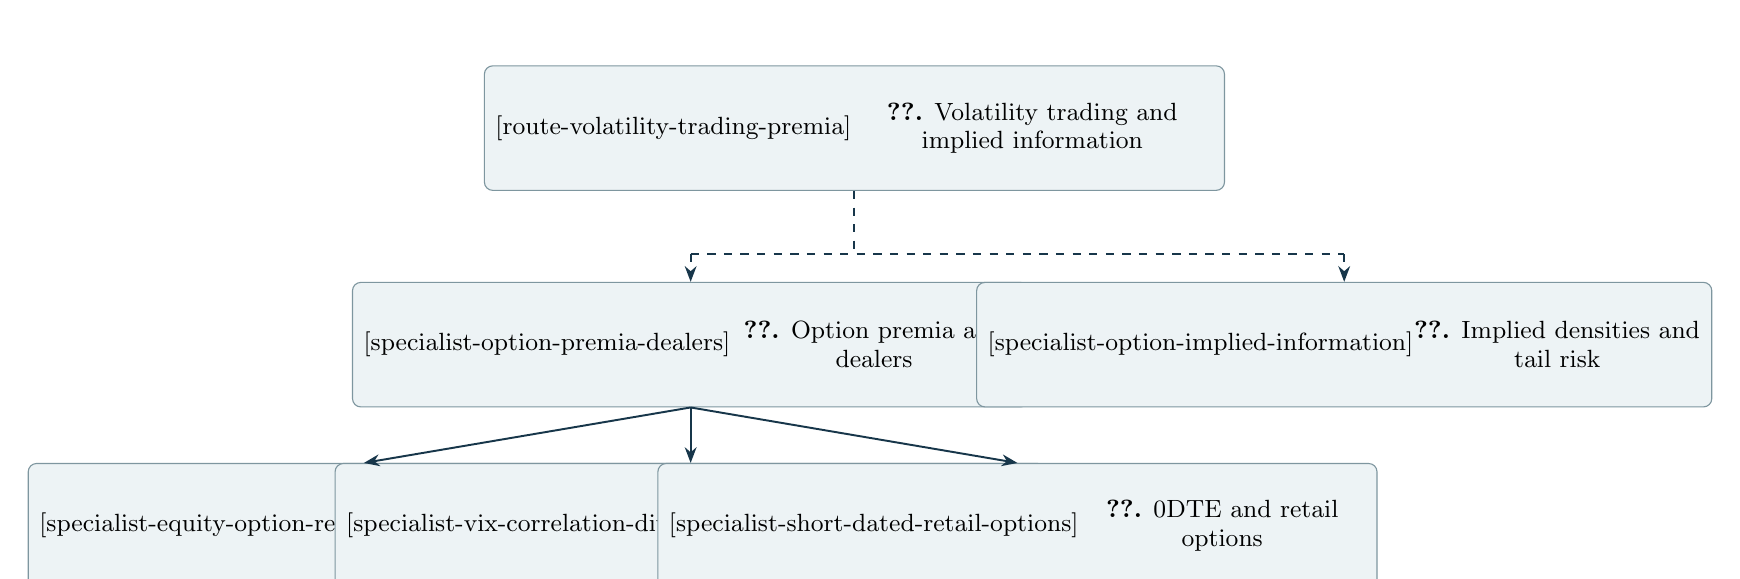
\begin{tikzpicture}[x=1cm,y=1cm]
\node[pathnode] (volatility-trading-premia) at (6.23,0) {\MeasurePathNode{4.6cm}{\textbf{\ref*{route-volatility-trading-premia}.} Volatility trading and implied information}\hyperref[route-volatility-trading-premia]{\parbox[c][\pathnodeheight][c]{4.6cm}{\centering \textbf{\ref*{route-volatility-trading-premia}.} Volatility trading and implied information}}};
\node[pathnode] (option-premia-dealers) at (4.15,-2.75) {\MeasurePathNode{3.65cm}{\textbf{\ref*{specialist-option-premia-dealers}.} Option premia and dealers}\hyperref[specialist-option-premia-dealers]{\parbox[c][\pathnodeheight][c]{3.65cm}{\centering \textbf{\ref*{specialist-option-premia-dealers}.} Option premia and dealers}}};
\node[pathnode] (option-implied-information) at (12.45,-2.75) {\MeasurePathNode{3.65cm}{\textbf{\ref*{specialist-option-implied-information}.} Implied densities and tail risk}\hyperref[specialist-option-implied-information]{\parbox[c][\pathnodeheight][c]{3.65cm}{\centering \textbf{\ref*{specialist-option-implied-information}.} Implied densities and tail risk}}};
\node[pathnode] (equity-option-returns) at (0.00,-5.05) {\MeasurePathNode{3.65cm}{\textbf{\ref*{specialist-equity-option-returns}.} Single-stock option returns}\hyperref[specialist-equity-option-returns]{\parbox[c][\pathnodeheight][c]{3.65cm}{\centering \textbf{\ref*{specialist-equity-option-returns}.} Single-stock option returns}}};
\node[pathnode] (vix-correlation-dividends) at (4.15,-5.05) {\MeasurePathNode{3.65cm}{\textbf{\ref*{specialist-vix-correlation-dividends}.} VIX, correlation and dividends}\hyperref[specialist-vix-correlation-dividends]{\parbox[c][\pathnodeheight][c]{3.65cm}{\centering \textbf{\ref*{specialist-vix-correlation-dividends}.} VIX, correlation and dividends}}};
\node[pathnode] (short-dated-retail-options) at (8.30,-5.05) {\MeasurePathNode{3.65cm}{\textbf{\ref*{specialist-short-dated-retail-options}.} 0DTE and retail options}\hyperref[specialist-short-dated-retail-options]{\parbox[c][\pathnodeheight][c]{3.65cm}{\centering \textbf{\ref*{specialist-short-dated-retail-options}.} 0DTE and retail options}}};
\draw[entryline] (volatility-trading-premia.south) -- (6.23,-1.60);
\draw[entryline] (4.15,-1.60) -- (12.45,-1.60);
\draw[entryarrow] (4.15,-1.60) -- (option-premia-dealers.north);
\draw[entryarrow] (12.45,-1.60) -- (option-implied-information.north);
\draw[patharrow] (option-premia-dealers.south) -- (equity-option-returns.north);
\draw[patharrow] (option-premia-dealers.south) -- (vix-correlation-dividends.north);
\draw[patharrow] (option-premia-dealers.south) -- (short-dated-retail-options.north);
\end{tikzpicture}\end{center}
\textbf{Bring these foundations with you.}\begin{itemize}
\item \hyperref[specialist-empirical-asset-pricing]{Empirical asset pricing: factor models and tests} --- needed by \hyperref[specialist-equity-option-returns]{Single-stock option returns}.
\end{itemize}\hyperref[learning-map]{Return to the whole-guide DAG.}
\Needspace{12\baselineskip}
\subsection{Option returns, variance premia and dealer hedging}\label{specialist-option-premia-dealers}
\textbf{Specialist pathway.} In \hyperref[route-volatility-trading-premia]{Volatility trading, option premia and implied information}.

\textbf{Outcome.} Replicate variance claims, measure variance and skew premia, and trace how dealer inventory and gamma hedging feed back into prices.

\textbf{Prerequisites.} Volatility trading, option premia and implied information overview; volatility surfaces.

\textbf{Review first.} \hyperref[route-volatility-trading-premia]{Volatility trading, option premia and implied information}.

\textbf{Required readings, in order}
\begin{enumerate}\raggedright
\Needspace{5\baselineskip}\item \href{institutional_quantitative_finance_reading_list.pdf\#wide-carr-madan-voltrading}{Peter Carr and Dilip Madan, ``Towards a theory of volatility trading''}\CataloguePage{131}\NoteKey{wide-carr-madan-voltrading}\par \textbf{Valuation.} Replicate volatility payoffs with option strips.
\Needspace{5\baselineskip}\item \href{institutional_quantitative_finance_reading_list.pdf\#wide-demeterfi-varswaps}{Kresimir Demeterfi, Emanuel Derman, Michael Kamal and Joseph Zou, ``A Guide to Volatility and Variance Swaps''}\CataloguePage{131}\NoteKey{wide-demeterfi-varswaps}\par \textbf{Mechanics.} Price and hedge variance swaps.
\Needspace{5\baselineskip}\item \href{institutional_quantitative_finance_reading_list.pdf\#wide-coval-shumway}{Joshua D. Coval and Tyler Shumway, ``Expected Option Returns''}\CataloguePage{131}\NoteKey{wide-coval-shumway}\par \textbf{Evidence.} Measure expected option returns.
\Needspace{5\baselineskip}\item \href{institutional_quantitative_finance_reading_list.pdf\#wide-bakshi-kapadia}{Gurdip Bakshi and Nikunj Kapadia, ``Delta-Hedged Gains and the Negative Market Volatility Risk Premium''}\CataloguePage{131}\NoteKey{wide-bakshi-kapadia}\par \textbf{Evidence.} Infer a negative volatility risk premium.
\Needspace{5\baselineskip}\item \href{institutional_quantitative_finance_reading_list.pdf\#gap-carr-wu-variance}{Peter Carr and Liuren Wu, Variance Risk Premiums}\CataloguePage{130}\NoteKey{gap-carr-wu-variance}\par \textbf{Evidence.} Measure variance risk premia across assets.
\Needspace{5\baselineskip}\item \href{institutional_quantitative_finance_reading_list.pdf\#wide-bollerslev-tauchen-zhou}{Tim Bollerslev, George Tauchen and Hao Zhou, ``Expected Stock Returns and Variance Risk Premia''}\CataloguePage{131}\NoteKey{wide-bollerslev-tauchen-zhou}\par \textbf{Evidence.} Use the variance premium to predict returns.
\Needspace{5\baselineskip}\item \href{institutional_quantitative_finance_reading_list.pdf\#wide-garleanu-pedersen-poteshman}{Nicolae Gârleanu, Lasse Heje Pedersen and Allen M. Poteshman, ``Demand-Based Option Pricing''}\CataloguePage{131}\NoteKey{wide-garleanu-pedersen-poteshman}\par \textbf{Theory.} Price end-user demand that dealers cannot hedge.
\Needspace{5\baselineskip}\item \href{institutional_quantitative_finance_reading_list.pdf\#wide-muravyev-order-flow}{Dmitriy Muravyev, ``Order Flow and Expected Option Returns''}\CataloguePage{131}\NoteKey{wide-muravyev-order-flow}\par \textbf{Evidence.} Relate order imbalance to option returns.
\Needspace{5\baselineskip}\item \href{institutional_quantitative_finance_reading_list.pdf\#wide-muravyev-pearson}{Dmitriy Muravyev and Neil D. Pearson, ``Options Trading Costs Are Lower than You Think''}\CataloguePage{132}\NoteKey{wide-muravyev-pearson}\par \textbf{Implementation.} Measure true option trading costs.
\Needspace{5\baselineskip}\item \href{institutional_quantitative_finance_reading_list.pdf\#wide-baltussen-hedging-demand}{Guido Baltussen, Zhi Da, Sten Lammers and Martin Martens, ``Hedging demand and market intraday momentum''}\CataloguePage{132}\NoteKey{wide-baltussen-hedging-demand}\par \textbf{Evidence.} Link dealer gamma to intraday momentum.
\Needspace{5\baselineskip}\item \href{institutional_quantitative_finance_reading_list.pdf\#wide-ni-pearson-poteshman-white}{Sophie X. Ni, Neil D. Pearson, Allen M. Poteshman and Joshua White, ``Does Option Trading Have a Pervasive Impact on Underlying Stock Prices?''}\CataloguePage{132}\NoteKey{wide-ni-pearson-poteshman-white}\par \textbf{Evidence.} Trace hedging effects on underlying volatility.
\end{enumerate}
\Needspace{5\baselineskip}\textbf{Checkpoint.} Compute a synthetic variance-swap rate from SPX options, estimate the variance premium and its predictive power, then compute daily dealer gamma estimates and test their relation to intraday reversal or momentum, reporting the data assumptions behind dealer positioning.

\textbf{Optional branches.} \href{institutional_quantitative_finance_reading_list.pdf\#wide-sinclair-positional}{Read a practitioner guide to harvesting option premia.}\BranchPage{139} \href{institutional_quantitative_finance_reading_list.pdf\#w4-khalfallah-volatility-carry}{Trade volatility carry across asset classes.}\BranchPage{131} \href{institutional_quantitative_finance_reading_list.pdf\#w5-israelov-nielsen-covered}{Decompose covered-call returns.}\BranchPage{140} \href{institutional_quantitative_finance_reading_list.pdf\#wide-dim-eraker-vilkov-0dte}{Test whether 0DTE dealer gamma destabilises the index.}\BranchPage{138} \href{institutional_quantitative_finance_reading_list.pdf\#w3-heston-variance-premium}{Isolate the variance premium with model-free option portfolios and check its seasonality.}\BranchPage{132} \href{institutional_quantitative_finance_reading_list.pdf\#vo-anderegg-ulmann-sornette-2022}{Measure how option dealers' short gamma raises FX spot volatility.}\BranchPage{132} \href{institutional_quantitative_finance_reading_list.pdf\#w5-whaley-bxm}{Benchmark systematic call overwriting with the BXM index.}\BranchPage{140}
\par{\small \hyperref[learning-map]{Learning pathway DAG} \textbar{} \hyperref[route-volatility-trading-premia]{Section overview} \textbar{} \hyperref[map-volatility-trading-premia]{Section DAG}\NoteKey{option-premia-dealers}}
\Needspace{12\baselineskip}
\subsection{Option-implied densities, tail risk and expected returns}\label{specialist-option-implied-information}
\textbf{Specialist pathway.} In \hyperref[route-volatility-trading-premia]{Volatility trading, option premia and implied information}.

\textbf{Outcome.} Extract risk-neutral densities, moments and tail measures from option prices, separate risk-neutral from physical beliefs where possible, and test their forecasting value out of sample.

\textbf{Prerequisites.} Volatility trading, option premia and implied information overview; volatility surfaces and no-arbitrage checks.

\textbf{Review first.} \hyperref[route-volatility-trading-premia]{Volatility trading, option premia and implied information}.

\textbf{Required readings, in order}
\begin{enumerate}\raggedright
\Needspace{5\baselineskip}\item \href{institutional_quantitative_finance_reading_list.pdf\#vo-christoffersen-jacobs-chang-2013}{Peter Christoffersen, Kris Jacobs and Bo Young Chang, ``Forecasting with Option-Implied Information''}\CataloguePage{140}\NoteKey{vo-christoffersen-jacobs-chang-2013}\par \textbf{Foundations.} Survey what option-implied volatility, moments and densities can and cannot forecast.
\Needspace{5\baselineskip}\item \href{institutional_quantitative_finance_reading_list.pdf\#wide-breeden-litzenberger}{Douglas T. Breeden and Robert H. Litzenberger, ``Prices of State-Contingent Claims Implicit in Option Prices''}\CataloguePage{118}\NoteKey{wide-breeden-litzenberger}\par \textbf{Theory.} Recover state prices from the second strike derivative of call prices.
\Needspace{5\baselineskip}\item \href{institutional_quantitative_finance_reading_list.pdf\#vo-jackwerth-rubinstein-1996}{Jens Carsten Jackwerth and Mark Rubinstein, ``Recovering Probability Distributions from Option Prices''}\CataloguePage{140}\NoteKey{vo-jackwerth-rubinstein-1996}\par \textbf{Methods.} Fit smooth implied distributions by optimisation and measure post-crash tail probabilities.
\Needspace{5\baselineskip}\item \href{institutional_quantitative_finance_reading_list.pdf\#vo-ait-sahalia-lo-1998}{Yacine Aït-Sahalia and Andrew W. Lo, ``Nonparametric Estimation of State-Price Densities Implicit in Financial Asset Prices''}\CataloguePage{140}\NoteKey{vo-ait-sahalia-lo-1998}\par \textbf{Methods.} Estimate state-price densities nonparametrically, with their sampling theory.
\Needspace{5\baselineskip}\item \href{institutional_quantitative_finance_reading_list.pdf\#vo-figlewski-2010}{Stephen Figlewski, ``Estimating the Implied Risk-Neutral Density for the US Market Portfolio''}\CataloguePage{141}\NoteKey{vo-figlewski-2010}\par \textbf{Implementation.} Build a complete density from bid--ask quotes and attach extreme-value tails.
\Needspace{5\baselineskip}\item \href{institutional_quantitative_finance_reading_list.pdf\#vo-jiang-tian-2005}{George J. Jiang and Yisong S. Tian, ``The Model-Free Implied Volatility and Its Information Content''}\CataloguePage{141}\NoteKey{vo-jiang-tian-2005}\par \textbf{Evidence.} Compute model-free implied variance and test it against Black--Scholes and realised volatility.
\Needspace{5\baselineskip}\item \href{institutional_quantitative_finance_reading_list.pdf\#vo-jackwerth-2000}{Jens Carsten Jackwerth, ``Recovering Risk Aversion from Option Prices and Realized Returns''}\CataloguePage{141}\NoteKey{vo-jackwerth-2000}\par \textbf{Evidence.} Combine implied and realised distributions to recover risk aversion and meet the pricing-kernel puzzle.
\Needspace{5\baselineskip}\item \href{institutional_quantitative_finance_reading_list.pdf\#vo-ross-2015}{Steve Ross, ``The Recovery Theorem''}\CataloguePage{141}\NoteKey{vo-ross-2015}\par \textbf{Theory.} Separate beliefs from risk aversion with the recovery theorem.
\Needspace{5\baselineskip}\item \href{institutional_quantitative_finance_reading_list.pdf\#vo-borovicka-hansen-scheinkman-2016}{Jaroslav Borovička, Lars Peter Hansen and José A. Scheinkman, ``Misspecified Recovery''}\CataloguePage{141}\NoteKey{vo-borovicka-hansen-scheinkman-2016}\par \textbf{Counter-evidence.} See why recovered probabilities can absorb long-term risk adjustments rather than reveal beliefs.
\Needspace{5\baselineskip}\item \href{institutional_quantitative_finance_reading_list.pdf\#w3-horvath-arbitrage-recovery}{Ferenc Horvath, ``Arbitrage-based recovery''}\CataloguePage{125}\NoteKey{w3-horvath-arbitrage-recovery}\par \textbf{Evidence.} Test a no-arbitrage recovery that needs state prices at only one maturity.
\Needspace{5\baselineskip}\item \href{institutional_quantitative_finance_reading_list.pdf\#vo-pan-2002}{Jun Pan, ``The Jump-Risk Premia Implicit in Options: Evidence from an Integrated Time-Series Study''}\CataloguePage{142}\NoteKey{vo-pan-2002}\par \textbf{Evidence.} Estimate jump-risk premia jointly from index returns and options.
\Needspace{5\baselineskip}\item \href{institutional_quantitative_finance_reading_list.pdf\#vo-bollerslev-todorov-2011}{Tim Bollerslev and Viktor Todorov, ``Tails, Fears, and Risk Premia''}\CataloguePage{142}\NoteKey{vo-bollerslev-todorov-2011}\par \textbf{Evidence.} Measure compensation for jump tails with an investor-fears index.
\Needspace{5\baselineskip}\item \href{institutional_quantitative_finance_reading_list.pdf\#vo-andersen-fusari-todorov-2015}{Torben G. Andersen, Nicola Fusari and Viktor Todorov, ``The Risk Premia Embedded in Index Options''}\CataloguePage{142}\NoteKey{vo-andersen-fusari-todorov-2015}\par \textbf{Evidence.} Identify a left-tail factor that predicts equity and variance premia but not volatility.
\Needspace{5\baselineskip}\item \href{institutional_quantitative_finance_reading_list.pdf\#wide-martin-svix}{Ian Martin, ``What is the Expected Return on the Market?''}\CataloguePage{31}\NoteKey{wide-martin-svix}\par \textbf{Evidence.} Bound the expected market return from index option prices.
\end{enumerate}
\Needspace{5\baselineskip}\textbf{Checkpoint.} For a month-end SPX option chain, fit an arbitrage-free smile, differentiate it twice to obtain the risk-neutral density, and attach extreme-value tails. From the same quotes compute model-free variance, skewness and kurtosis, the SVIX lower bound and a left-tail measure. Over at least ten years of month-ends, test whether these predict next-month realised variance and excess returns out of sample, and report how the results change with strike truncation, interpolation and tail choice.

\textbf{Optional branches.} \href{institutional_quantitative_finance_reading_list.pdf\#vo-britten-jones-neuberger-2000}{Derive the model-free volatility forecast from current option prices alone.}\BranchPage{140} \href{institutional_quantitative_finance_reading_list.pdf\#vo-bliss-panigirtzoglou-2004}{Estimate risk aversion by adjusting the risk-neutral density with a utility function.}\BranchPage{141} \href{institutional_quantitative_finance_reading_list.pdf\#vo-martin-wagner-2019}{Extend the SVIX bound to the expected returns of individual stocks.}\BranchPage{142} \href{institutional_quantitative_finance_reading_list.pdf\#vo-kelly-pastor-veronesi-2016}{Price political-event risk in options that span elections and summits.}\BranchPage{142} \href{institutional_quantitative_finance_reading_list.pdf\#vo-bollinger-melick-thomas-2023}{Attach density tails that also price the options at the attachment strikes.}\BranchPage{141} \href{institutional_quantitative_finance_reading_list.pdf\#wide-kelly-jiang-tail}{Compare a tail-risk measure from stock returns with option-implied tails.}\BranchPage{104} \href{institutional_quantitative_finance_reading_list.pdf\#w3-xian-risk-neutral-gen}{Generate arbitrage-free risk-neutral densities with neural networks.}\BranchPage{129}
\par{\small \hyperref[learning-map]{Learning pathway DAG} \textbar{} \hyperref[route-volatility-trading-premia]{Section overview} \textbar{} \hyperref[map-volatility-trading-premia]{Section DAG}\NoteKey{option-implied-information}}
\Needspace{12\baselineskip}
\subsection{Single-stock option returns: volatility mispricing, characteristics and factors}\label{specialist-equity-option-returns}
\textbf{Specialist pathway.} In \hyperref[route-volatility-trading-premia]{Volatility trading, option premia and implied information}.

\textbf{Outcome.} Measure delta-hedged single-stock option returns, test volatility, skew, earnings and firm-characteristic predictors, and explain them with option factor models net of trading costs.

\textbf{Prerequisites.} Option returns, variance premia and dealer hedging; empirical asset pricing and factor tests.

\textbf{Review first.} \hyperref[specialist-option-premia-dealers]{Option returns, variance premia and dealer hedging}; \hyperref[specialist-empirical-asset-pricing]{Empirical asset pricing: factor models and tests}.

\textbf{Required readings, in order}
\begin{enumerate}\raggedright
\Needspace{5\baselineskip}\item \href{institutional_quantitative_finance_reading_list.pdf\#vo-christoffersen-fournier-jacobs-2018}{Peter Christoffersen, Mathieu Fournier and Kris Jacobs, ``The Factor Structure in Equity Options''}\CataloguePage{132}\NoteKey{vo-christoffersen-fournier-jacobs-2018}\par \textbf{Foundations.} See that equity implied-volatility levels, skews and term structures share strong common factors tied to the index.
\Needspace{5\baselineskip}\item \href{institutional_quantitative_finance_reading_list.pdf\#vo-goyal-saretto-2009}{Amit Goyal and Alessio Saretto, ``Cross-Section of Option Returns and Volatility''}\CataloguePage{133}\NoteKey{vo-goyal-saretto-2009}\par \textbf{Evidence.} Sort on historical-minus-implied volatility to find mispriced stock options.
\Needspace{5\baselineskip}\item \href{institutional_quantitative_finance_reading_list.pdf\#vo-cao-han-2013}{Jie Cao and Bing Han, ``Cross Section of Option Returns and Idiosyncratic Stock Volatility''}\CataloguePage{133}\NoteKey{vo-cao-han-2013}\par \textbf{Evidence.} See delta-hedged option returns fall with idiosyncratic volatility, linked to dealers' arbitrage costs.
\Needspace{5\baselineskip}\item \href{institutional_quantitative_finance_reading_list.pdf\#vo-vasquez-2017}{Aurelio Vasquez, ``Equity Volatility Term Structures and the Cross Section of Option Returns''}\CataloguePage{133}\NoteKey{vo-vasquez-2017}\par \textbf{Evidence.} Use the slope of the implied-volatility term structure to predict straddle returns.
\Needspace{5\baselineskip}\item \href{institutional_quantitative_finance_reading_list.pdf\#vo-bali-murray-2013}{Turan G. Bali and Scott Murray, ``Does Risk-Neutral Skewness Predict the Cross-Section of Equity Option Portfolio Returns?''}\CataloguePage{133}\NoteKey{vo-bali-murray-2013}\par \textbf{Evidence.} Isolate risk-neutral skewness with delta- and vega-neutral skewness assets.
\Needspace{5\baselineskip}\item \href{institutional_quantitative_finance_reading_list.pdf\#vo-ni-pan-poteshman-2008}{Sophie X. Ni, Jun Pan and Allen M. Poteshman, ``Volatility Information Trading in the Option Market''}\CataloguePage{133}\NoteKey{vo-ni-pan-poteshman-2008}\par \textbf{Evidence.} Trace informed volatility demand and its price impact before earnings announcements.
\Needspace{5\baselineskip}\item \href{institutional_quantitative_finance_reading_list.pdf\#vo-dubinsky-johannes-kaeck-seeger-2019}{Andrew Dubinsky, Michael Johannes, Andreas Kaeck and Norman J. Seeger, ``Option Pricing of Earnings Announcement Risks''}\CataloguePage{133}\NoteKey{vo-dubinsky-johannes-kaeck-seeger-2019}\par \textbf{Valuation.} Separate earnings-announcement uncertainty from normal volatility in option prices.
\Needspace{5\baselineskip}\item \href{institutional_quantitative_finance_reading_list.pdf\#vo-zhan-han-cao-tong-2022}{Xintong (Eunice) Zhan, Bing Han, Jie Cao and Qing Tong, ``Option Return Predictability''}\CataloguePage{134}\NoteKey{vo-zhan-han-cao-tong-2022}\par \textbf{Evidence.} Test firm characteristics that predict delta-hedged option returns after costs.
\Needspace{5\baselineskip}\item \href{institutional_quantitative_finance_reading_list.pdf\#vo-bali-beckmeyer-moerke-weigert-2023}{Turan G. Bali, Heiner Beckmeyer, Mathis Mörke and Florian Weigert, ``Option Return Predictability with Machine Learning and Big Data''}\CataloguePage{134}\NoteKey{vo-bali-beckmeyer-moerke-weigert-2023}\par \textbf{Methods.} Predict option returns with nonlinear machine learning on option and stock characteristics.
\Needspace{5\baselineskip}\item \href{institutional_quantitative_finance_reading_list.pdf\#w3-horenstein-option-factors}{Alex Horenstein, Aurelio Vasquez and Xiao Xiao, ``Common Factors in Equity Option Returns''}\CataloguePage{134}\NoteKey{w3-horenstein-option-factors}\par \textbf{Evidence.} Price delta-hedged option returns with a small set of common factors.
\Needspace{5\baselineskip}\item \href{institutional_quantitative_finance_reading_list.pdf\#vo-goyal-saretto-2025}{Amit Goyal and Alessio Saretto, ``Can Equity Option Returns Be Explained by a Factor Model? IPCA Says Yes''}\CataloguePage{134}\NoteKey{vo-goyal-saretto-2025}\par \textbf{Validation.} Check whether an IPCA factor model explains 46 option anomalies before trading one.
\Needspace{5\baselineskip}\item \href{institutional_quantitative_finance_reading_list.pdf\#wide-christoffersen-option-illiquidity}{Peter Christoffersen, Ruslan Goyenko, Kris Jacobs and Mehdi Karoui, ``Illiquidity Premia in the Equity Options Market''}\CataloguePage{132}\NoteKey{wide-christoffersen-option-illiquidity}\par \textbf{Implementation.} Account for illiquidity premia and spreads in any option anomaly return.
\end{enumerate}
\Needspace{5\baselineskip}\textbf{Checkpoint.} Build a monthly panel of 30-day at-the-money delta-hedged calls and straddles on liquid U.S. stocks. Form portfolios on historical-minus-implied volatility, idiosyncratic volatility, term-structure slope and risk-neutral skewness; report returns at mid-quotes and at effective spreads, treat earnings-announcement months separately, and test whether an IPCA or option-factor model explains the returns.

\textbf{Optional branches.} \href{institutional_quantitative_finance_reading_list.pdf\#vo-gao-xing-zhang-2018}{Test straddles bought just before earnings announcements.}\BranchPage{133} \href{institutional_quantitative_finance_reading_list.pdf\#vo-dennis-mayhew-2002}{Explain the cross-section of stock-option skews.}\BranchPage{132} \href{institutional_quantitative_finance_reading_list.pdf\#w3-boulatov-cheap-options}{See retail demand make cheap options expensive.}\BranchPage{135} \href{institutional_quantitative_finance_reading_list.pdf\#w3-muravyev-options-info}{Link implied-volatility signals to stock-borrow fees.}\BranchPage{135} \href{institutional_quantitative_finance_reading_list.pdf\#vo-muravyev-pearson-pollet-2022}{Check whether option-implied borrow fees carry a risk premium.}\BranchPage{135} \href{institutional_quantitative_finance_reading_list.pdf\#w4-alexiou-concave-iv}{Read event risk from concave implied-volatility curves.}\BranchPage{134} \href{institutional_quantitative_finance_reading_list.pdf\#w3-kafer-option-factor-momentum}{Test momentum in option factor returns.}\BranchPage{134} \href{institutional_quantitative_finance_reading_list.pdf\#w3-kafer-bayesian-option-sdf}{Price option anomalies with a Bayesian stochastic discount factor.}\BranchPage{134} \href{institutional_quantitative_finance_reading_list.pdf\#w3-wu-zhang-linear-option}{Price single-stock options top-down with a linear model.}\BranchPage{134}
\par{\small \hyperref[learning-map]{Learning pathway DAG} \textbar{} \hyperref[route-volatility-trading-premia]{Section overview} \textbar{} \hyperref[map-volatility-trading-premia]{Section DAG}\NoteKey{equity-option-returns}}
\Needspace{12\baselineskip}
\subsection{VIX, correlation and dividend derivatives}\label{specialist-vix-correlation-dividends}
\textbf{Specialist pathway.} In \hyperref[route-volatility-trading-premia]{Volatility trading, option premia and implied information}.

\textbf{Outcome.} Price and hedge VIX futures and options, correlation and dispersion trades and dividend claims, measure their premia, and see how settlement rules and product design can fail.

\textbf{Prerequisites.} Option returns, variance premia and dealer hedging; variance-swap replication.

\textbf{Review first.} \hyperref[specialist-option-premia-dealers]{Option returns, variance premia and dealer hedging}.

\textbf{Required readings, in order}
\begin{enumerate}\raggedright
\Needspace{5\baselineskip}\item \href{institutional_quantitative_finance_reading_list.pdf\#vo-whaley-2009}{Robert E. Whaley, ``Understanding the VIX''}\CataloguePage{135}\NoteKey{vo-whaley-2009}\par \textbf{Mechanics.} Read what the VIX measures and what it does not.
\Needspace{5\baselineskip}\item \href{institutional_quantitative_finance_reading_list.pdf\#gap-cboe-vix6}{Cboe Global Indices, Cboe Volatility Index Methodology}\CataloguePage{135}\NoteKey{gap-cboe-vix6}\par \textbf{Data.} Reproduce VIX inputs, strike selection and maturity conventions from the current methodology.
\Needspace{5\baselineskip}\item \href{institutional_quantitative_finance_reading_list.pdf\#vo-mencia-sentana-2013}{Javier Mencía and Enrique Sentana, ``Valuation of VIX Derivatives''}\CataloguePage{135}\NoteKey{vo-mencia-sentana-2013}\par \textbf{Valuation.} Compare VIX futures and option pricing models before, during and after 2008.
\Needspace{5\baselineskip}\item \href{institutional_quantitative_finance_reading_list.pdf\#gap-vix-premium}{Ing-Haw Cheng, The VIX Premium}\CataloguePage{135}\NoteKey{gap-vix-premium}\par \textbf{Evidence.} Measure the VIX futures premium against expected VIX and link it to hedging demand.
\Needspace{5\baselineskip}\item \href{institutional_quantitative_finance_reading_list.pdf\#vo-eraker-wu-2017}{Bjørn Eraker and Yue Wu, ``Explaining the Negative Returns to Volatility Claims: An Equilibrium Approach''}\CataloguePage{136}\NoteKey{vo-eraker-wu-2017}\par \textbf{Evidence.} Explain the steep negative returns to long VIX futures and ETNs in equilibrium.
\Needspace{5\baselineskip}\item \href{institutional_quantitative_finance_reading_list.pdf\#vo-augustin-cheng-van-den-bergen-2021}{Patrick Augustin, Ing-Haw Cheng and Ludovic Van den Bergen, ``Volmageddon and the Failure of Short Volatility Products''}\CataloguePage{136}\NoteKey{vo-augustin-cheng-van-den-bergen-2021}\par \textbf{Evidence.} Trace the February 2018 collapse of short-volatility ETPs to hedge and leverage rebalancing.
\Needspace{5\baselineskip}\item \href{institutional_quantitative_finance_reading_list.pdf\#vo-griffin-shams-2018}{John M. Griffin and Amin Shams, ``Manipulation in the VIX?''}\CataloguePage{136}\NoteKey{vo-griffin-shams-2018}\par \textbf{Evidence.} Test whether settlement-day SPX option volume is consistent with VIX manipulation.
\Needspace{5\baselineskip}\item \href{institutional_quantitative_finance_reading_list.pdf\#w5-bossu-advanced-equity}{Sébastien Bossu, \emph{Advanced Equity Derivatives: Volatility and Correlation}}\CataloguePage{139}\NoteKey{w5-bossu-advanced-equity}\par \textbf{Mechanics.} Learn variance, volatility, dispersion and correlation products and their replication.
\Needspace{5\baselineskip}\item \href{institutional_quantitative_finance_reading_list.pdf\#gap-correlation-risk}{Joost Driessen, Pascal J. Maenhout and Grigory Vilkov, The Price of Correlation Risk: Evidence from Equity Options}\CataloguePage{130}\NoteKey{gap-correlation-risk}\par \textbf{Evidence.} Price correlation risk from index and constituent options.
\Needspace{5\baselineskip}\item \href{institutional_quantitative_finance_reading_list.pdf\#vo-buss-vilkov-2012}{Adrian Buss and Grigory Vilkov, ``Measuring Equity Risk with Option-Implied Correlations''}\CataloguePage{130}\NoteKey{vo-buss-vilkov-2012}\par \textbf{Methods.} Construct option-implied correlations and forward-looking betas.
\Needspace{5\baselineskip}\item \href{institutional_quantitative_finance_reading_list.pdf\#vo-bondarenko-bernard-2024}{Oleg Bondarenko and Carole Bernard, ``Option-Implied Dependence and Correlation Risk Premium''}\CataloguePage{130}\NoteKey{vo-bondarenko-bernard-2024}\par \textbf{Evidence.} Separate the premia on down-market and up-market correlation using sector and index options.
\Needspace{5\baselineskip}\item \href{institutional_quantitative_finance_reading_list.pdf\#gap-dividend-strips}{Jules van Binsbergen, Michael Brandt and Ralph Koijen, On the Timing and Pricing of Dividends}\CataloguePage{136}\NoteKey{gap-dividend-strips}\par \textbf{Evidence.} Extract short-horizon dividend claims and the term structure of equity risk.
\Needspace{5\baselineskip}\item \href{institutional_quantitative_finance_reading_list.pdf\#gap-dividend-comment}{Florian Schulz, On the Timing and Pricing of Dividends: Comment}\CataloguePage{136}\NoteKey{gap-dividend-comment}\par \textbf{Counter-evidence.} Check how frictions and measurement change the dividend-strip result.
\Needspace{5\baselineskip}\item \href{institutional_quantitative_finance_reading_list.pdf\#vo-van-binsbergen-hueskes-koijen-vrugt-2013}{Jules van Binsbergen, Wouter Hueskes, Ralph Koijen and Evert Vrugt, ``Equity Yields''}\CataloguePage{136}\NoteKey{vo-van-binsbergen-hueskes-koijen-vrugt-2013}\par \textbf{Evidence.} Build equity yields from traded dividends in the U.S., Europe and Japan.
\Needspace{5\baselineskip}\item \href{institutional_quantitative_finance_reading_list.pdf\#vo-bansal-miller-song-yaron-2021}{Ravi Bansal, Shane Miller, Dongho Song and Amir Yaron, ``The Term Structure of Equity Risk Premia''}\CataloguePage{137}\NoteKey{vo-bansal-miller-song-yaron-2021}\par \textbf{Counter-evidence.} See the slope of dividend risk premia change sign over the business cycle.
\end{enumerate}
\Needspace{5\baselineskip}\textbf{Checkpoint.} From daily VIX futures settlements, compute the roll yield and returns of constant-maturity long and short VIX positions, and reproduce the 5 February 2018 loss of an inverse VIX product from its published rebalancing rule. Separately, compute implied correlation from SPX and sector or constituent options and the return of a delta-hedged dispersion trade through at least one stress episode. From Euro Stoxx 50 dividend futures, compute equity yields by maturity and compare implied with realised dividends.

\textbf{Optional branches.} \href{institutional_quantitative_finance_reading_list.pdf\#vo-gormsen-2021}{See the slope of the equity term structure move with the cycle.}\BranchPage{137} \href{institutional_quantitative_finance_reading_list.pdf\#vo-kragt-de-jong-driessen-2020}{Fit a two-factor model to Euro Stoxx 50 dividend futures.}\BranchPage{137} \href{institutional_quantitative_finance_reading_list.pdf\#vo-ulrich-florig-seehuber-2023}{Estimate U.S. dividend premiums from options and analysts' forecasts.}\BranchPage{137} \href{institutional_quantitative_finance_reading_list.pdf\#vo-alexander-korovilas-kapraun-2016}{Test whether volatility futures diversify portfolios after roll and trading costs.}\BranchPage{136} \href{institutional_quantitative_finance_reading_list.pdf\#w4-bangsgaard-kokholm-vix-hedging}{Trace VIX ETP hedging into SPX futures.}\BranchPage{136} \href{institutional_quantitative_finance_reading_list.pdf\#w5-carr-lee-volderivs}{Review volatility-derivative replication.}\BranchPage{139}
\par{\small \hyperref[learning-map]{Learning pathway DAG} \textbar{} \hyperref[route-volatility-trading-premia]{Section overview} \textbar{} \hyperref[map-volatility-trading-premia]{Section DAG}\NoteKey{vix-correlation-dividends}}
\Needspace{12\baselineskip}
\subsection{Short-dated options, 0DTE and retail option trading}\label{specialist-short-dated-retail-options}
\textbf{Specialist pathway.} In \hyperref[route-volatility-trading-premia]{Volatility trading, option premia and implied information}.

\textbf{Outcome.} Price weekly and same-day index options, test whether their trading and dealer hedging move index volatility, and measure what retail option traders pay and lose.

\textbf{Prerequisites.} Option returns, variance premia and dealer hedging; high-frequency volatility measurement.

\textbf{Review first.} \hyperref[specialist-option-premia-dealers]{Option returns, variance premia and dealer hedging}.

\textbf{Required readings, in order}
\begin{enumerate}\raggedright
\Needspace{5\baselineskip}\item \href{institutional_quantitative_finance_reading_list.pdf\#vo-andersen-fusari-todorov-2017}{Torben G. Andersen, Nicola Fusari and Viktor Todorov, ``Short-Term Market Risks Implied by Weekly Options''}\CataloguePage{137}\NoteKey{vo-andersen-fusari-todorov-2017}\par \textbf{Evidence.} Read negative jump-tail risk from weekly options, separately from volatility.
\Needspace{5\baselineskip}\item \href{institutional_quantitative_finance_reading_list.pdf\#wide-bandi-0dte}{Federico M. Bandi, Nicola Fusari and Roberto Renò, ``0DTE Option Pricing''}\CataloguePage{137}\NoteKey{wide-bandi-0dte}\par \textbf{Valuation.} Price same-day options with intraday volatility and jumps.
\Needspace{5\baselineskip}\item \href{institutional_quantitative_finance_reading_list.pdf\#w4-todorov-zhang-intraday-vol}{Viktor Todorov and Yang Zhang, ``Intraday volatility patterns from short-dated options''}\CataloguePage{137}\NoteKey{w4-todorov-zhang-intraday-vol}\par \textbf{Methods.} Recover intraday volatility patterns from short-dated options.
\Needspace{5\baselineskip}\item \href{institutional_quantitative_finance_reading_list.pdf\#w3-chong-todorov-0dte}{Carsten H. Chong and Viktor Todorov, ``Do Equity and Options Markets Agree about Volatility?''}\CataloguePage{137}\NoteKey{w3-chong-todorov-0dte}\par \textbf{Evidence.} Test whether same-day options and the stock market agree about volatility.
\Needspace{5\baselineskip}\item \href{institutional_quantitative_finance_reading_list.pdf\#vo-almeida-freire-hizmeri-2024}{Caio Almeida, Gustavo Freire and Rodrigo Hizmeri, ``0DTE Asset Pricing''}\CataloguePage{138}\NoteKey{vo-almeida-freire-hizmeri-2024}\par \textbf{Evidence.} Compare 0DTE variance premia and price-bound violations with longer maturities.
\Needspace{5\baselineskip}\item \href{institutional_quantitative_finance_reading_list.pdf\#wide-dim-eraker-vilkov-0dte}{Chukwuma Dim, Bjørn Eraker and Grigory Vilkov, ``0DTEs: Trading, Gamma Risk and Volatility Propagation''}\CataloguePage{138}\NoteKey{wide-dim-eraker-vilkov-0dte}\par \textbf{Evidence.} Test whether 0DTE dealer gamma propagates index volatility.
\Needspace{5\baselineskip}\item \href{institutional_quantitative_finance_reading_list.pdf\#vo-brogaard-han-won-2023}{Jonathan Brogaard, Jaehee Han and Peter Y. Won, ``Does 0DTE Options Trading Increase Volatility?''}\CataloguePage{138}\NoteKey{vo-brogaard-han-won-2023}\par \textbf{Counter-evidence.} Weigh instrumental-variable evidence that 0DTE trading raises volatility.
\Needspace{5\baselineskip}\item \href{institutional_quantitative_finance_reading_list.pdf\#vo-lakonishok-lee-pearson-poteshman-2007}{Josef Lakonishok, Inmoo Lee, Neil D. Pearson and Allen M. Poteshman, ``Option Market Activity''}\CataloguePage{138}\NoteKey{vo-lakonishok-lee-pearson-poteshman-2007}\par \textbf{Evidence.} Describe who buys and who writes options, by investor class.
\Needspace{5\baselineskip}\item \href{institutional_quantitative_finance_reading_list.pdf\#vo-bauer-cosemans-eichholtz-2009}{Rob Bauer, Mathijs Cosemans and Piet Eichholtz, ``Option Trading and Individual Investor Performance''}\CataloguePage{138}\NoteKey{vo-bauer-cosemans-eichholtz-2009}\par \textbf{Evidence.} Measure individual investors' option losses and their causes.
\Needspace{5\baselineskip}\item \href{institutional_quantitative_finance_reading_list.pdf\#ex-bryzgalova-pavlova-sikorskaya-2023}{Svetlana Bryzgalova, Anna Pavlova and Taisiya Sikorskaya, ``Retail Trading in Options and the Rise of the Big Three Wholesalers''}\CataloguePage{174}\NoteKey{ex-bryzgalova-pavlova-sikorskaya-2023}\par \textbf{Evidence.} Measure retail options flow routed through wholesalers and what it costs.
\Needspace{5\baselineskip}\item \href{institutional_quantitative_finance_reading_list.pdf\#vo-de-silva-smith-so-2023}{Tim de Silva, Kevin Smith and Eric C. So, ``Losing is Optional: Retail Option Trading and Expected Announcement Volatility''}\CataloguePage{139}\NoteKey{vo-de-silva-smith-so-2023}\par \textbf{Evidence.} See retail buyers overpay for options before earnings announcements.
\Needspace{5\baselineskip}\item \href{institutional_quantitative_finance_reading_list.pdf\#vo-beckmeyer-branger-gayda-2023}{Heiner Beckmeyer, Nicole Branger and Leander Gayda, ``Retail Traders Love 0DTE Options\ldots{} But Should They?''}\CataloguePage{139}\NoteKey{vo-beckmeyer-branger-gayda-2023}\par \textbf{Evidence.} Identify retail 0DTE trades through price-improvement auctions and measure their losses.
\Needspace{5\baselineskip}\item \href{institutional_quantitative_finance_reading_list.pdf\#w3-eaton-retail-options-iv}{Gregory W. Eaton, T. Clifton Green, Brian S. Roseman and Yanbin Wu, ``Retail option traders and the implied volatility surface''}\CataloguePage{138}\NoteKey{w3-eaton-retail-options-iv}\par \textbf{Evidence.} See retail option demand shape the implied-volatility surface.
\Needspace{5\baselineskip}\item \href{institutional_quantitative_finance_reading_list.pdf\#exp-egebjerg-0dte-hedging}{Sebastian Egebjerg, Deep hedging 0DTE options}\CataloguePage{128}\NoteKey{exp-egebjerg-0dte-hedging}\par \textbf{Implementation.} Compare learned and delta hedges for same-day options under real costs.
\end{enumerate}
\Needspace{5\baselineskip}\textbf{Checkpoint.} Using at least a year of intraday SPX 0DTE quotes and trades, compute the same-day variance premium from 10:00 ET to the close, estimate market makers' aggregate gamma under stated assumptions about who is on each side, and test whether it predicts intraday index volatility or reversals. Separately, estimate retail option traders' returns at their execution prices with a stated retail-flow classifier, and split the loss into spread, premium and timing.

\textbf{Optional branches.} \href{institutional_quantitative_finance_reading_list.pdf\#vo-vilkov-2023}{Test 0DTE timing rules under a strict out-of-sample protocol.}\BranchPage{138}
\par{\small \hyperref[learning-map]{Learning pathway DAG} \textbar{} \hyperref[route-volatility-trading-premia]{Section overview} \textbar{} \hyperref[map-volatility-trading-premia]{Section DAG}\NoteKey{short-dated-retail-options}}
\clearpage
\section{Multi-asset and systematic macro}\label{route-multi-asset-systematic-macro}
\label{route-3}
\textbf{Learning sequence.} Start with cross-asset style premia, trend following, risk parity and macro announcements; macro regimes and the stock–bond correlation build on risk parity, and nowcasting builds on announcements. Currencies follow in their own section.

\textbf{Section goals.} Across its pathways, this section teaches you to:
\begin{itemize}[leftmargin=1.4em,itemsep=0pt,topsep=1pt]
\item build and judge value, momentum, carry and defensive premia across asset classes (\hyperref[specialist-cross-asset-style-premia]{\ref*{specialist-cross-asset-style-premia}})
\item construct and evaluate diversified trend-following strategies (\hyperref[specialist-trend-following]{\ref*{specialist-trend-following}})
\item build risk-parity and volatility-targeted portfolios and decide their leverage (\hyperref[specialist-risk-parity-vol-targeting]{\ref*{specialist-risk-parity-vol-targeting}})
\item measure asset-price responses and premia around macro announcements and policy news (\hyperref[specialist-macro-announcements-policy]{\ref*{specialist-macro-announcements-policy}})
\item identify macro regimes in real time and model the stock--bond correlation (\hyperref[specialist-macro-regimes-stock-bond]{\ref*{specialist-macro-regimes-stock-bond}})
\item build real-time nowcasts and macro trading signals without look-ahead (\hyperref[specialist-macro-nowcasting-signals]{\ref*{specialist-macro-nowcasting-signals}})
\end{itemize}
\textbf{Overview outcome.} Attribute a cross-asset portfolio's returns to carry, trend, value and rate exposures, using signals built from release vintages and tradable contract rolls, and show how funding haircuts, trading costs and a rapid unwind change the result.

\textbf{Prerequisites.} Common toolkit; futures, bond duration and collateral mechanics. Currencies follow in the next section.

\textbf{Review first.} \hyperref[route-common-toolkit]{Common toolkit}.

\textbf{Required readings, in order}
\begin{enumerate}\raggedright
\Needspace{5\baselineskip}\item \href{institutional_quantitative_finance_reading_list.pdf\#s7-ilmanen}{Antti Ilmanen, \emph{Expected Returns}}\CataloguePage{31}\NoteKey{s7-ilmanen}\par Map expected returns to risk premia and the limits of historical cross-asset comparisons.
\Needspace{5\baselineskip}\item \href{institutional_quantitative_finance_reading_list.pdf\#wide-dimson-marsh-staunton}{Elroy Dimson, Paul Marsh and Mike Staunton, \emph{Triumph of the Optimists: 101 Years of Global Investment Returns}}\CataloguePage{32}\NoteKey{wide-dimson-marsh-staunton}\par Set long-run base rates for equities, bonds, bills and currencies across countries before trusting a short sample.
\Needspace{5\baselineskip}\item \href{institutional_quantitative_finance_reading_list.pdf\#alpha-carry}{Ralph Koijen, Tobias Moskowitz, Lasse Heje Pedersen and Evert Vrugt, ``Carry''}\CataloguePage{30}\NoteKey{alpha-carry}\par Define carry consistently across assets before interpreting it as expected return.
\Needspace{5\baselineskip}\item \href{institutional_quantitative_finance_reading_list.pdf\#s6-tsmom}{Tobias Moskowitz, Yao Hua Ooi and Lasse Heje Pedersen, ``Time Series Momentum''}\CataloguePage{30}\NoteKey{s6-tsmom}\par Contrast trend exposure with carry and understand the path dependence of crisis behavior.
\Needspace{5\baselineskip}\item \href{institutional_quantitative_finance_reading_list.pdf\#s16-r11}{Macrosynergy, \emph{Macroeconomic Data and Systematic Trading Strategies} (2024)}\CataloguePage{268}\NoteKey{s16-r11}\par Build macro signals from release calendars and revisions, not final revised series.
\Needspace{5\baselineskip}\item \href{institutional_quantitative_finance_reading_list.pdf\#exp-adrian-crump-moench-term-structure}{Tobias Adrian, Richard K. Crump, and Emanuel Moench, Pricing the Term Structure with Linear Regressions; New York Fed ACM term-premium data notes}\CataloguePage{214}\NoteKey{exp-adrian-crump-moench-term-structure}\par Decompose a bond yield into expected short rates and estimated term premium.
\Needspace{5\baselineskip}\item \href{institutional_quantitative_finance_reading_list.pdf\#exp-brunnermeier-pedersen-liquidity}{Markus K. Brunnermeier and Lasse Heje Pedersen, Market Liquidity and Funding Liquidity}\CataloguePage{177}\NoteKey{exp-brunnermeier-pedersen-liquidity}\par Model the feedback between funding constraints and the liquidity available to unwind positions.
\Needspace{5\baselineskip}\item \href{institutional_quantitative_finance_reading_list.pdf\#exp-garleanu-pedersen-dynamic-costs}{Nicolae Gârleanu and Lasse Heje Pedersen, Dynamic Trading with Predictable Returns and Transaction Costs; author manuscript}\CataloguePage{99}\NoteKey{exp-garleanu-pedersen-dynamic-costs}\par Translate forecasts into paced trades when signals decay and transaction costs matter.
\end{enumerate}
\Needspace{5\baselineskip}\textbf{Checkpoint.} Build a dated cross-asset signal panel using release vintages and tradable contract rolls. Attribute one portfolio's returns to carry, trend, value and rate exposures, then rerun with funding haircuts, transaction costs and a rapid unwind.

\textbf{Optional branches.} \href{institutional_quantitative_finance_reading_list.pdf\#section.13.1}{Explore systematic macro practice, books and history in more depth.}\BranchPage{264} \href{institutional_quantitative_finance_reading_list.pdf\#section.11.1}{Deepen term-premium and bond-liquidity research.}\BranchPage{212} \href{institutional_quantitative_finance_reading_list.pdf\#latest-financial-econometrics}{Deepen a specific high-frequency, trend, factor or volatility-inference method after standard econometrics.}\BranchPage{36} \href{institutional_quantitative_finance_reading_list.pdf\#wide-ilmanen-low-returns}{Revisit expected returns, factor premia and alternatives when markets offer little.}\BranchPage{265} \href{institutional_quantitative_finance_reading_list.pdf\#wide-willer-saunders-macro}{Read a 2026 practitioner text on trading macro regimes across rates, FX, equities and emerging markets.}\BranchPage{265} \href{institutional_quantitative_finance_reading_list.pdf\#s7-drobny}{Compare systematic rules with how discretionary macro managers frame trades.}\BranchPage{264} \href{institutional_quantitative_finance_reading_list.pdf\#s7-soros}{Use reflexivity between beliefs, prices, policy and financing to frame stress scenarios.}\BranchPage{264} \href{institutional_quantitative_finance_reading_list.pdf\#s7-reinhart}{Place current debt and crisis indicators in eight centuries of history.}\BranchPage{264}
\par\textbf{Continue in this section.} \hyperref[specialist-cross-asset-style-premia]{Cross-asset style premia: value, momentum, carry and defensive}; \hyperref[specialist-trend-following]{Trend following and managed futures}; \hyperref[specialist-risk-parity-vol-targeting]{Risk parity, leverage and volatility targeting}; \hyperref[specialist-macro-announcements-policy]{Macro announcements, policy news and announcement premia}; \hyperref[specialist-macro-regimes-stock-bond]{Macro regimes, inflation and the stock–bond correlation}; \hyperref[specialist-macro-nowcasting-signals]{Nowcasting, real-time macro data and macro trading signals}.
\par{\small \hyperref[learning-map]{Learning pathway DAG} \textbar{} \hyperref[map-multi-asset-systematic-macro]{Section DAG}\NoteKey{multi-asset-systematic-macro}}
\clearpage
\subsection*{Multi-asset and systematic macro: pathway DAG}\phantomsection\label{map-multi-asset-systematic-macro}
\addcontentsline{toc}{subsection}{Multi-asset and systematic macro: pathway DAG}
Start with the section overview's readings, for orientation. Solid arrows show prerequisites within this section. Dashed connectors identify entry points with no further prerequisite in this section; the linked foundations below still apply. Follow the arrows for dependencies and the subsection numbers for reading order. Every node is clickable.
\begin{center}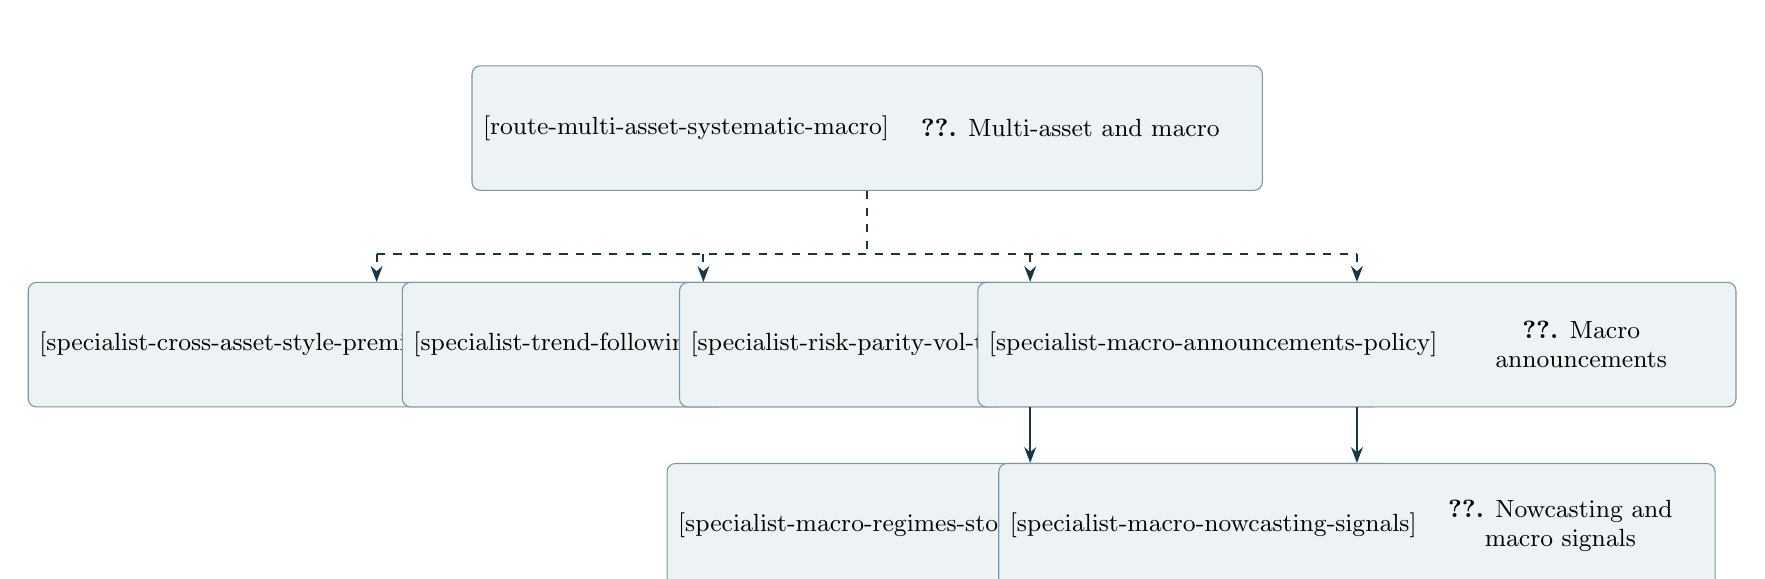
\begin{tikzpicture}[x=1cm,y=1cm]
\node[pathnode] (multi-asset-systematic-macro) at (6.23,0) {\MeasurePathNode{4.6cm}{\textbf{\ref*{route-multi-asset-systematic-macro}.} Multi-asset and macro}\hyperref[route-multi-asset-systematic-macro]{\parbox[c][\pathnodeheight][c]{4.6cm}{\centering \textbf{\ref*{route-multi-asset-systematic-macro}.} Multi-asset and macro}}};
\node[pathnode] (cross-asset-style-premia) at (0.00,-2.75) {\MeasurePathNode{3.65cm}{\textbf{\ref*{specialist-cross-asset-style-premia}.} Cross-asset style premia}\hyperref[specialist-cross-asset-style-premia]{\parbox[c][\pathnodeheight][c]{3.65cm}{\centering \textbf{\ref*{specialist-cross-asset-style-premia}.} Cross-asset style premia}}};
\node[pathnode] (trend-following) at (4.15,-2.75) {\MeasurePathNode{3.65cm}{\textbf{\ref*{specialist-trend-following}.} Trend following}\hyperref[specialist-trend-following]{\parbox[c][\pathnodeheight][c]{3.65cm}{\centering \textbf{\ref*{specialist-trend-following}.} Trend following}}};
\node[pathnode] (risk-parity-vol-targeting) at (8.30,-2.75) {\MeasurePathNode{3.65cm}{\textbf{\ref*{specialist-risk-parity-vol-targeting}.} Risk parity and volatility targeting}\hyperref[specialist-risk-parity-vol-targeting]{\parbox[c][\pathnodeheight][c]{3.65cm}{\centering \textbf{\ref*{specialist-risk-parity-vol-targeting}.} Risk parity and volatility targeting}}};
\node[pathnode] (macro-announcements-policy) at (12.45,-2.75) {\MeasurePathNode{3.65cm}{\textbf{\ref*{specialist-macro-announcements-policy}.} Macro announcements}\hyperref[specialist-macro-announcements-policy]{\parbox[c][\pathnodeheight][c]{3.65cm}{\centering \textbf{\ref*{specialist-macro-announcements-policy}.} Macro announcements}}};
\node[pathnode] (macro-regimes-stock-bond) at (8.30,-5.05) {\MeasurePathNode{3.65cm}{\textbf{\ref*{specialist-macro-regimes-stock-bond}.} Regimes, inflation and stock–bond correlation}\hyperref[specialist-macro-regimes-stock-bond]{\parbox[c][\pathnodeheight][c]{3.65cm}{\centering \textbf{\ref*{specialist-macro-regimes-stock-bond}.} Regimes, inflation and stock–bond correlation}}};
\node[pathnode] (macro-nowcasting-signals) at (12.45,-5.05) {\MeasurePathNode{3.65cm}{\textbf{\ref*{specialist-macro-nowcasting-signals}.} Nowcasting and macro signals}\hyperref[specialist-macro-nowcasting-signals]{\parbox[c][\pathnodeheight][c]{3.65cm}{\centering \textbf{\ref*{specialist-macro-nowcasting-signals}.} Nowcasting and macro signals}}};
\draw[entryline] (multi-asset-systematic-macro.south) -- (6.23,-1.60);
\draw[entryline] (0.00,-1.60) -- (12.45,-1.60);
\draw[entryarrow] (0.00,-1.60) -- (cross-asset-style-premia.north);
\draw[entryarrow] (4.15,-1.60) -- (trend-following.north);
\draw[entryarrow] (8.30,-1.60) -- (risk-parity-vol-targeting.north);
\draw[entryarrow] (12.45,-1.60) -- (macro-announcements-policy.north);
\draw[patharrow] (risk-parity-vol-targeting.south) -- (macro-regimes-stock-bond.north);
\draw[patharrow] (macro-announcements-policy.south) -- (macro-nowcasting-signals.north);
\end{tikzpicture}\end{center}
\textbf{Bring these foundations with you.}\begin{itemize}
\item \hyperref[specialist-empirical-asset-pricing]{Empirical asset pricing: factor models and tests} --- needed by \hyperref[specialist-cross-asset-style-premia]{Cross-asset style premia}.
\item \hyperref[specialist-time-series-volatility]{Time-series econometrics and volatility forecasting} --- needed by \hyperref[specialist-trend-following]{Trend following}, \hyperref[specialist-risk-parity-vol-targeting]{Risk parity and volatility targeting}, \hyperref[specialist-macro-announcements-policy]{Macro announcements}, \hyperref[specialist-macro-regimes-stock-bond]{Regimes, inflation and stock–bond correlation}, \hyperref[specialist-macro-nowcasting-signals]{Nowcasting and macro signals}.
\item \hyperref[specialist-point-in-time-data]{Point-in-time data, vendor files and bias control} --- needed by \hyperref[specialist-macro-nowcasting-signals]{Nowcasting and macro signals}.
\end{itemize}\hyperref[learning-map]{Return to the whole-guide DAG.}
\Needspace{12\baselineskip}
\subsection{Cross-asset style premia: value, momentum, carry and defensive}\label{specialist-cross-asset-style-premia}
\textbf{Specialist pathway.} In \hyperref[route-multi-asset-systematic-macro]{Multi-asset and systematic macro}.

\textbf{Outcome.} Build value, momentum, carry and defensive strategies in equity indices, bonds, currencies and commodities, judge them against a century of out-of-sample evidence, and decide how far to time them.

\textbf{Prerequisites.} Multi-asset overview; empirical asset pricing.

\textbf{Review first.} \hyperref[route-multi-asset-systematic-macro]{Multi-asset and systematic macro}; \hyperref[specialist-empirical-asset-pricing]{Empirical asset pricing: factor models and tests}.

\textbf{Required readings, in order}
\begin{enumerate}\raggedright
\Needspace{5\baselineskip}\item \href{institutional_quantitative_finance_reading_list.pdf\#alpha-value}{Clifford Asness, Tobias Moskowitz and Lasse Heje Pedersen, ``Value and Momentum Everywhere'' (author copy)}\CataloguePage{192}\NoteKey{alpha-value}\par \textbf{Evidence.} Find value and momentum premia, and their negative correlation, across markets and asset classes.
\Needspace{5\baselineskip}\item \href{institutional_quantitative_finance_reading_list.pdf\#s16-r37}{Brian Hurst, Yao Hua Ooi and Lasse Heje Pedersen, \emph{Understanding Managed Futures} (2010); Clifford Asness, Antti Ilmanen, Ronen Israel and Tobias Moskowitz, \emph{Investing with Style}, \emph{Journal of Investment Management} (2015)}\CataloguePage{266}\NoteKey{s16-r37}\par \textbf{Foundations.} Use Investing with Style for multi-asset definitions of value, momentum, carry and defensive.
\Needspace{5\baselineskip}\item \href{institutional_quantitative_finance_reading_list.pdf\#ma-asness-liew-stevens-1997}{Clifford S. Asness, John M. Liew and Ross L. Stevens, ``Parallels Between the Cross-Sectional Predictability of Stock and Country Returns''}\CataloguePage{265}\NoteKey{ma-asness-liew-stevens-1997}\par \textbf{Evidence.} Apply value, size and momentum to countries rather than stocks.
\Needspace{5\baselineskip}\item \href{institutional_quantitative_finance_reading_list.pdf\#wide-ilmanen-century-factors}{Antti S. Ilmanen, Ronen Israel, Tobias J. Moskowitz, Ashwin K. Thapar and Franklin Wang, ``Factor Premia and Factor Timing: A Century of Evidence''}\CataloguePage{194}\NoteKey{wide-ilmanen-century-factors}\par \textbf{Evidence.} Test style premia across asset classes over a century.
\Needspace{5\baselineskip}\item \href{institutional_quantitative_finance_reading_list.pdf\#w5-baltussen-global-premiums}{Guido Baltussen, Laurens Swinkels and Pim van Vliet, ``Global factor premiums''}\CataloguePage{194}\NoteKey{w5-baltussen-global-premiums}\par \textbf{Validation.} Check global premia out of sample over two centuries after allowing for p-hacking.
\Needspace{5\baselineskip}\item \href{institutional_quantitative_finance_reading_list.pdf\#alpha-bab}{Andrea Frazzini and Lasse Heje Pedersen, ``Betting Against Beta''}\CataloguePage{192}\NoteKey{alpha-bab}\par \textbf{Evidence.} See a low-beta premium within bonds, credit, currencies and commodities as well as equities.
\Needspace{5\baselineskip}\item \href{institutional_quantitative_finance_reading_list.pdf\#ma-lettau-maggiori-weber-2014}{Martin Lettau, Matteo Maggiori and Michael Weber, ``Conditional risk premia in currency markets and other asset classes''}\CataloguePage{265}\NoteKey{ma-lettau-maggiori-weber-2014}\par \textbf{Theory.} Price carry across asset classes with downside market risk.
\Needspace{5\baselineskip}\item \href{institutional_quantitative_finance_reading_list.pdf\#ma-pitkajarvi-suominen-vaittinen-2020}{Aleksi Pitkäjärvi, Matti Suominen and Lauri Vaittinen, ``Cross-asset signals and time series momentum''}\CataloguePage{265}\NoteKey{ma-pitkajarvi-suominen-vaittinen-2020}\par \textbf{Evidence.} Use bond momentum to time equities and equity momentum to time bonds.
\Needspace{5\baselineskip}\item \href{institutional_quantitative_finance_reading_list.pdf\#s16-r16}{David Blitz and Pim van Vliet, \emph{Global Tactical Cross-Asset Allocation: Applying Value and Momentum Across Asset Classes} (2008)}\CataloguePage{268}\NoteKey{s16-r16}\par \textbf{Implementation.} Allocate tactically across asset classes with value and momentum.
\Needspace{5\baselineskip}\item \href{institutional_quantitative_finance_reading_list.pdf\#ma-baltas-2019}{Nick Baltas, ``The Impact of Crowding in Alternative Risk Premia Investing''}\CataloguePage{266}\NoteKey{ma-baltas-2019}\par \textbf{Implementation.} Anticipate how crowding affects divergence and convergence premia.
\Needspace{5\baselineskip}\item \href{institutional_quantitative_finance_reading_list.pdf\#ma-haddad-kozak-santosh-2020}{Valentin Haddad, Serhiy Kozak and Shrihari Santosh, ``Factor Timing''}\CataloguePage{266}\NoteKey{ma-haddad-kozak-santosh-2020}\par \textbf{Methods.} Time factors through the stochastic discount factor.
\Needspace{5\baselineskip}\item \href{institutional_quantitative_finance_reading_list.pdf\#ma-asness-chandra-ilmanen-israel-2017}{Clifford Asness, Swati Chandra, Antti Ilmanen and Ronen Israel, ``Contrarian Factor Timing is Deceptively Difficult''}\CataloguePage{266}\NoteKey{ma-asness-chandra-ilmanen-israel-2017}\par \textbf{Counter-evidence.} See why value-spread timing adds little to a multi-style portfolio.
\end{enumerate}
\Needspace{5\baselineskip}\textbf{Checkpoint.} Build value, 12-month momentum, carry and low-beta signals for equity-index, government-bond, currency and commodity futures since 1990. Combine them with equal risk weights, report each style's correlation with the others and with equities, and compare a static allocation with one timed by value spreads, net of costs.

\textbf{Optional branches.} \href{institutional_quantitative_finance_reading_list.pdf\#ma-bhojraj-swaminathan-2006}{Add currency effects to country-index momentum and reversal.}\BranchPage{265} \href{institutional_quantitative_finance_reading_list.pdf\#ma-gupta-kelly-2019}{Time equity factors with their own momentum.}\BranchPage{266} \href{institutional_quantitative_finance_reading_list.pdf\#exp-factor-timing-shrinkage}{Shrink a high-dimensional factor-timing portfolio toward skepticism.}\BranchPage{54} \href{institutional_quantitative_finance_reading_list.pdf\#s16-r17}{Read a practitioner account of twelve systematic global macro strategies.}\BranchPage{268} \href{institutional_quantitative_finance_reading_list.pdf\#wide-adrian-etula-muir}{Price many asset classes with broker-dealer leverage.}\BranchPage{33} \href{institutional_quantitative_finance_reading_list.pdf\#wide-he-krishnamurthy}{Model risk premia that rise when intermediaries are capital constrained.}\BranchPage{33} \href{institutional_quantitative_finance_reading_list.pdf\#s7-lo}{Read why premia and strategy returns change as competitors adapt.}\BranchPage{264}
\par{\small \hyperref[learning-map]{Learning pathway DAG} \textbar{} \hyperref[route-multi-asset-systematic-macro]{Section overview} \textbar{} \hyperref[map-multi-asset-systematic-macro]{Section DAG}\NoteKey{cross-asset-style-premia}}
\Needspace{12\baselineskip}
\subsection{Trend following and managed futures}\label{specialist-trend-following}
\textbf{Specialist pathway.} In \hyperref[route-multi-asset-systematic-macro]{Multi-asset and systematic macro}.

\textbf{Outcome.} Construct a diversified trend strategy with volatility targeting, costs and crisis evaluation, and weigh the contrary evidence.

\textbf{Prerequisites.} Multi-asset overview and time-series econometrics.

\textbf{Review first.} \hyperref[route-multi-asset-systematic-macro]{Multi-asset and systematic macro}; \hyperref[specialist-time-series-volatility]{Time-series econometrics and volatility forecasting}.

\textbf{Required readings, in order}
\begin{enumerate}\raggedright
\Needspace{5\baselineskip}\item \href{institutional_quantitative_finance_reading_list.pdf\#s6-tsmom}{Tobias Moskowitz, Yao Hua Ooi and Lasse Heje Pedersen, ``Time Series Momentum''}\CataloguePage{30}\NoteKey{s6-tsmom}\par \textbf{Evidence.} Read the core time-series momentum evidence.
\Needspace{5\baselineskip}\item \href{institutional_quantitative_finance_reading_list.pdf\#alpha-century}{Brian Hurst, Yao Hua Ooi and Lasse Heje Pedersen, ``A Century of Evidence on Trend-Following Investing''}\CataloguePage{30}\NoteKey{alpha-century}\par \textbf{Evidence.} Extend to a century of data.
\Needspace{5\baselineskip}\item \href{institutional_quantitative_finance_reading_list.pdf\#wide-lemperiere-two-centuries}{Yves Lempérière, Cyril Deremble, Philip Seager, Marc Potters and Jean-Philippe Bouchaud, ``Two centuries of trend following''}\CataloguePage{267}\NoteKey{wide-lemperiere-two-centuries}\par \textbf{Evidence.} Check two centuries of trends.
\Needspace{5\baselineskip}\item \href{institutional_quantitative_finance_reading_list.pdf\#wide-levine-pedersen-trend}{Ari Levine and Lasse Heje Pedersen, ``Which Trend Is Your Friend?''}\CataloguePage{267}\NoteKey{wide-levine-pedersen-trend}\par \textbf{Theory.} Unify moving averages and TSMOM.
\Needspace{5\baselineskip}\item \href{institutional_quantitative_finance_reading_list.pdf\#s16-r43}{William Fung and David A. Hsieh, \emph{The Risk in Hedge Fund Strategies: Theory and Evidence from Trend Followers} (2001); \emph{Asset-Based Style Factors for Hedge Funds} (2002); \emph{Hedge Fund Benchmarks: A Risk-Based Approach} (2004)}\CataloguePage{267}\NoteKey{s16-r43}\par \textbf{Theory.} Model trend-follower returns as lookback straddles and build asset-based benchmarks.
\Needspace{5\baselineskip}\item \href{institutional_quantitative_finance_reading_list.pdf\#wide-baltas-kosowski}{Nick Baltas and Robert Kosowski, ``Demystifying Time-Series Momentum Strategies: Volatility Estimators, Trading Rules and Pairwise Correlations''}\CataloguePage{267}\NoteKey{wide-baltas-kosowski}\par \textbf{Implementation.} Choose volatility estimators and signal rules.
\Needspace{5\baselineskip}\item \href{institutional_quantitative_finance_reading_list.pdf\#wide-kim-tse-wald}{Abby Y. Kim, Yiuman Tse and John K. Wald, ``Time series momentum and volatility scaling''}\CataloguePage{267}\NoteKey{wide-kim-tse-wald}\par \textbf{Counter-evidence.} Separate volatility scaling from the trend signal.
\Needspace{5\baselineskip}\item \href{institutional_quantitative_finance_reading_list.pdf\#wide-huang-tsmom-there}{Dashan Huang, Jiangyuan Li, Liyao Wang and Guofu Zhou, ``Time series momentum: Is it there?''}\CataloguePage{267}\NoteKey{wide-huang-tsmom-there}\par \textbf{Counter-evidence.} Test asset-by-asset predictability.
\Needspace{5\baselineskip}\item \href{institutional_quantitative_finance_reading_list.pdf\#ma-bhardwaj-gorton-rouwenhorst-2014}{Geetesh Bhardwaj, Gary B. Gorton and K. Geert Rouwenhorst, ``Fooling Some of the People All of the Time: The Inefficient Performance and Persistence of Commodity Trading Advisors''}\CataloguePage{268}\NoteKey{ma-bhardwaj-gorton-rouwenhorst-2014}\par \textbf{Counter-evidence.} Compare CTA returns net of fees with simple futures strategies.
\Needspace{5\baselineskip}\item \href{institutional_quantitative_finance_reading_list.pdf\#wide-harvey-vol-targeting}{Campbell R. Harvey, Edward Hoyle, Russell Korgaonkar, Sandy Rattray, Matthew Sargaison and Otto Van Hemert, ``The Impact of Volatility Targeting''}\CataloguePage{107}\NoteKey{wide-harvey-vol-targeting}\par \textbf{Implementation.} Assess volatility targeting by asset class.
\Needspace{5\baselineskip}\item \href{institutional_quantitative_finance_reading_list.pdf\#wide-babu-trends-everywhere}{Abhilash Babu, Ari Levine, Yao Hua Ooi, Lasse Heje Pedersen and Erik Stamelos, ``Trends Everywhere''}\CataloguePage{267}\NoteKey{wide-babu-trends-everywhere}\par \textbf{Evidence.} Extend trends to alternative markets.
\Needspace{5\baselineskip}\item \href{institutional_quantitative_finance_reading_list.pdf\#wide-harvey-worst-times}{Campbell R. Harvey, Edward Hoyle, Sandy Rattray, Matthew Sargaison, Dan Taylor and Otto Van Hemert, ``The Best of Strategies for the Worst of Times: Can Portfolios Be Crisis Proofed?''}\CataloguePage{104}\NoteKey{wide-harvey-worst-times}\par \textbf{Evidence.} Compare trend with other crisis hedges.
\Needspace{5\baselineskip}\item \href{institutional_quantitative_finance_reading_list.pdf\#ma-goulding-harvey-mazzoleni-2023}{Christian L. Goulding, Campbell R. Harvey and Michele G. Mazzoleni, ``Momentum turning points''}\CataloguePage{267}\NoteKey{ma-goulding-harvey-mazzoleni-2023}\par \textbf{Methods.} Blend slow and fast momentum around market turning points.
\Needspace{5\baselineskip}\item \href{institutional_quantitative_finance_reading_list.pdf\#wide-carver-afts}{Robert Carver, \emph{Advanced Futures Trading Strategies: 30 Fully Tested Strategies for Multiple Trading Styles and Time Frames}}\CataloguePage{267}\NoteKey{wide-carver-afts}\par \textbf{Implementation.} Implement sizing, carry and cost-aware futures systems.
\Needspace{5\baselineskip}\item \href{institutional_quantitative_finance_reading_list.pdf\#w4-hood-raughtigan-voltarget-trend}{Benjamin T. Hood and Cameron Raughtigan, ``Volatility Targeting Is Trendy: How Trend Following Explains Alpha in Volatility-Managed Strategies''}\CataloguePage{107}\NoteKey{w4-hood-raughtigan-voltarget-trend}\par \textbf{Evidence.} See volatility-targeting alpha reduce to an implicit trend loading in equities.
\end{enumerate}
\Needspace{5\baselineskip}\textbf{Checkpoint.} Build a 40-market trend portfolio with continuous futures, volatility targeting and realistic costs; report performance in the worst equity drawdowns, compare with a pure volatility-scaled long portfolio, and test asset-level predictability as Huang et al. propose.

\textbf{Optional branches.} \href{institutional_quantitative_finance_reading_list.pdf\#s16-r39}{Read Man Group work on trend drawdowns.}\BranchPage{266} \href{institutional_quantitative_finance_reading_list.pdf\#s16-r26}{Compare crisis-alpha perspectives.}\BranchPage{266} \href{institutional_quantitative_finance_reading_list.pdf\#s7-carver}{Follow a practical progression from single rules to a combined system.}\BranchPage{266} \href{institutional_quantitative_finance_reading_list.pdf\#wide-fung-hsieh-biases}{Check survivorship and backfill bias before using CTA index returns.}\BranchPage{520}
\par{\small \hyperref[learning-map]{Learning pathway DAG} \textbar{} \hyperref[route-multi-asset-systematic-macro]{Section overview} \textbar{} \hyperref[map-multi-asset-systematic-macro]{Section DAG}\NoteKey{trend-following}}
\Needspace{12\baselineskip}
\subsection{Risk parity, leverage and volatility targeting}\label{specialist-risk-parity-vol-targeting}
\textbf{Specialist pathway.} In \hyperref[route-multi-asset-systematic-macro]{Multi-asset and systematic macro}.

\textbf{Outcome.} Construct equal-risk-contribution and volatility-targeted multi-asset portfolios, decide how much leverage they need, and test whether volatility scaling improves returns out of sample and after costs.

\textbf{Prerequisites.} Multi-asset overview; volatility forecasting. Portfolio construction and risk (Part III) treats estimation error and optimisation in more depth.

\textbf{Review first.} \hyperref[route-multi-asset-systematic-macro]{Multi-asset and systematic macro}; \hyperref[specialist-time-series-volatility]{Time-series econometrics and volatility forecasting}.

\textbf{Required readings, in order}
\begin{enumerate}\raggedright
\Needspace{5\baselineskip}\item \href{institutional_quantitative_finance_reading_list.pdf\#s16-r07}{Bridgewater, \emph{The All Weather Story} (2012); Bob Prince, IPE interview (2011)}\CataloguePage{107}\NoteKey{s16-r07}\par \textbf{Foundations.} See risk balanced across growth and inflation environments, and the leverage it needs.
\Needspace{5\baselineskip}\item \href{institutional_quantitative_finance_reading_list.pdf\#s16-r24}{Edward Qian, \emph{Risk Parity Portfolios: Efficient Portfolios Through True Diversification} (September 2005); Roger Clarke, Harindra de Silva and Steven Thorley, \emph{Risk Parity, Maximum Diversification, and Minimum Variance: An Analytic Perspective} (2013)}\CataloguePage{107}\NoteKey{s16-r24}\par \textbf{Theory.} Compare risk parity, maximum diversification and minimum variance analytically.
\Needspace{5\baselineskip}\item \href{institutional_quantitative_finance_reading_list.pdf\#wide-maillard-roncalli-erc}{Sébastien Maillard, Thierry Roncalli and Jérôme Teïletche, ``The Properties of Equally Weighted Risk Contribution Portfolios''}\CataloguePage{98}\NoteKey{wide-maillard-roncalli-erc}\par \textbf{Methods.} Define equal-risk-contribution portfolios.
\Needspace{5\baselineskip}\item \href{institutional_quantitative_finance_reading_list.pdf\#wide-roncalli-risk-parity}{Thierry Roncalli, \emph{Introduction to Risk Parity and Budgeting}}\CataloguePage{98}\NoteKey{wide-roncalli-risk-parity}\par \textbf{Methods.} Compute risk budgets for multi-asset portfolios.
\Needspace{5\baselineskip}\item \href{institutional_quantitative_finance_reading_list.pdf\#wide-choueifaty-coignard}{Yves Choueifaty and Yves Coignard, ``Toward Maximum Diversification''}\CataloguePage{98}\NoteKey{wide-choueifaty-coignard}\par \textbf{Methods.} Maximise the diversification ratio as an alternative risk-based rule.
\Needspace{5\baselineskip}\item \href{institutional_quantitative_finance_reading_list.pdf\#audit-lee}{Wai Lee, \emph{Risk-Based Asset Allocation: A New Answer to an Old Question?}, \emph{Journal of Portfolio Management} 37(4), 11--28 (Summer 2011)}\CataloguePage{106}\NoteKey{audit-lee}\par \textbf{Theory.} Check which return assumptions each risk-based rule implies.
\Needspace{5\baselineskip}\item \href{institutional_quantitative_finance_reading_list.pdf\#w2-asness-leverage-aversion}{Clifford S. Asness, Andrea Frazzini and Lasse H. Pedersen, ``Leverage Aversion and Risk Parity''}\CataloguePage{268}\NoteKey{w2-asness-leverage-aversion}\par \textbf{Evidence.} Explain the returns of levered risk parity by leverage aversion.
\Needspace{5\baselineskip}\item \href{institutional_quantitative_finance_reading_list.pdf\#w2-anderson-risk-parity}{Robert M. Anderson, Stephen W. Bianchi and Lisa R. Goldberg, ``Will My Risk Parity Strategy Outperform?''}\CataloguePage{268}\NoteKey{w2-anderson-risk-parity}\par \textbf{Counter-evidence.} Test risk parity's sensitivity to sample period, financing and trading costs.
\Needspace{5\baselineskip}\item \href{institutional_quantitative_finance_reading_list.pdf\#w5-chaves-risk-parity}{Denis Chaves, Jason Hsu, Feifei Li and Omid Shakernia, ``Risk Parity Portfolio vs. Other Asset Allocation Heuristic Portfolios''}\CataloguePage{99}\NoteKey{w5-chaves-risk-parity}\par \textbf{Evidence.} Compare risk parity with equal weight, minimum variance and 60/40.
\Needspace{5\baselineskip}\item \href{institutional_quantitative_finance_reading_list.pdf\#ma-bollerslev-hood-huss-pedersen-2018}{Tim Bollerslev, Benjamin Hood, John Huss and Lasse Heje Pedersen, ``Risk Everywhere: Modeling and Managing Volatility''}\CataloguePage{108}\NoteKey{ma-bollerslev-hood-huss-pedersen-2018}\par \textbf{Methods.} Forecast volatility across asset classes with panel realised-volatility models.
\Needspace{5\baselineskip}\item \href{institutional_quantitative_finance_reading_list.pdf\#s16-r25}{Alan Moreira and Tyler Muir, \emph{Volatility-Managed Portfolios}, \emph{Journal of Finance} (2017)}\CataloguePage{107}\NoteKey{s16-r25}\par \textbf{Evidence.} Scale factor exposure inversely to recent variance.
\Needspace{5\baselineskip}\item \href{institutional_quantitative_finance_reading_list.pdf\#wide-cederburg-volmanaged}{Scott Cederburg, Michael S. O'Doherty, Feifei Wang and Xuemin (Sterling) Yan, ``On the performance of volatility-managed portfolios''}\CataloguePage{107}\NoteKey{wide-cederburg-volmanaged}\par \textbf{Counter-evidence.} Test volatility management out of sample across 103 strategies.
\Needspace{5\baselineskip}\item \href{institutional_quantitative_finance_reading_list.pdf\#ma-demiguel-martin-utrera-uppal-2024}{Victor DeMiguel, Alberto Martín-Utrera and Raman Uppal, ``A Multifactor Perspective on Volatility-Managed Portfolios''}\CataloguePage{108}\NoteKey{ma-demiguel-martin-utrera-uppal-2024}\par \textbf{Evidence.} Manage volatility jointly across factors, out of sample and net of costs.
\Needspace{5\baselineskip}\item \href{institutional_quantitative_finance_reading_list.pdf\#ma-bongaerts-kang-van-dijk-2020}{Dion Bongaerts, Xiaowei Kang and Mathijs van Dijk, ``Conditional Volatility Targeting''}\CataloguePage{108}\NoteKey{ma-bongaerts-kang-van-dijk-2020}\par \textbf{Implementation.} Target volatility only in extreme volatility states.
\end{enumerate}
\Needspace{5\baselineskip}\textbf{Checkpoint.} Build a four-asset portfolio of equity, nominal-bond, inflation-linked-bond and commodity futures since 1990. Compare equal-weight, 60/40, equal-risk-contribution and maximum-diversification weights, lever risk parity to the 60/40 volatility with realistic financing, then add constant and conditional volatility targeting and report Sharpe ratios, drawdowns and turnover net of costs.

\textbf{Optional branches.} \href{institutional_quantitative_finance_reading_list.pdf\#alpha-scherer}{Follow risk budgeting alongside views, scenarios and costs.}\BranchPage{107} \href{institutional_quantitative_finance_reading_list.pdf\#s16-r38}{Read a practitioner framework that separates alpha from beta and economic environments.}\BranchPage{107} \href{institutional_quantitative_finance_reading_list.pdf\#wide-harvey-vol-targeting}{Assess volatility targeting asset class by asset class.}\BranchPage{107} \href{institutional_quantitative_finance_reading_list.pdf\#s7-dalio}{Read a manager's view of diversification across return streams.}\BranchPage{107}
\par{\small \hyperref[learning-map]{Learning pathway DAG} \textbar{} \hyperref[route-multi-asset-systematic-macro]{Section overview} \textbar{} \hyperref[map-multi-asset-systematic-macro]{Section DAG}\NoteKey{risk-parity-vol-targeting}}
\Needspace{12\baselineskip}
\subsection{Macro announcements, policy news and announcement premia}\label{specialist-macro-announcements-policy}
\textbf{Specialist pathway.} In \hyperref[route-multi-asset-systematic-macro]{Multi-asset and systematic macro}.

\textbf{Outcome.} Measure how stocks, bonds and currencies respond to scheduled macro releases and FOMC decisions, explain why the responses change over the business cycle, and estimate how much of the equity premium is earned around announcements.

\textbf{Prerequisites.} Multi-asset overview; time-series econometrics. Monetary policy, balance-sheet policy and the yield curve (section 5) treats policy-surprise construction and asset purchases in more depth.

\textbf{Review first.} \hyperref[route-multi-asset-systematic-macro]{Multi-asset and systematic macro}; \hyperref[specialist-time-series-volatility]{Time-series econometrics and volatility forecasting}.

\textbf{Required readings, in order}
\begin{enumerate}\raggedright
\Needspace{5\baselineskip}\item \href{institutional_quantitative_finance_reading_list.pdf\#wide-abdv-announcements}{Torben G. Andersen, Tim Bollerslev, Francis X. Diebold and Clara Vega, ``Micro Effects of Macro Announcements: Real-Time Price Discovery in Foreign Exchange''}\CataloguePage{271}\NoteKey{wide-abdv-announcements}\par \textbf{Evidence.} Study high-frequency FX responses to news.
\Needspace{5\baselineskip}\item \href{institutional_quantitative_finance_reading_list.pdf\#ma-andersen-bollerslev-diebold-vega-2007}{Torben G. Andersen, Tim Bollerslev, Francis X. Diebold and Clara Vega, ``Real-time price discovery in global stock, bond and foreign exchange markets''}\CataloguePage{271}\NoteKey{ma-andersen-bollerslev-diebold-vega-2007}\par \textbf{Evidence.} Extend announcement responses to stocks and bonds in three countries and across the business cycle.
\Needspace{5\baselineskip}\item \href{institutional_quantitative_finance_reading_list.pdf\#ma-boyd-hu-jagannathan-2005}{John H. Boyd, Jian Hu and Ravi Jagannathan, ``The Stock Market's Reaction to Unemployment News: Why Bad News Is Usually Good for Stocks''}\CataloguePage{272}\NoteKey{ma-boyd-hu-jagannathan-2005}\par \textbf{Evidence.} See why bad unemployment news is usually good for stocks in expansions.
\Needspace{5\baselineskip}\item \href{institutional_quantitative_finance_reading_list.pdf\#ma-elenev-law-song-yaron-2024}{Vadim Elenev, Tzuo-Hann Law, Dongho Song and Amir Yaron, ``Fearing the Fed: How wall street reads main street''}\CataloguePage{272}\NoteKey{ma-elenev-law-song-yaron-2024}\par \textbf{Evidence.} Explain the countercyclical sensitivity of stocks to macro news.
\Needspace{5\baselineskip}\item \href{institutional_quantitative_finance_reading_list.pdf\#ma-gilbert-scotti-strasser-vega-2017}{Thomas Gilbert, Chiara Scotti, Georg Strasser and Clara Vega, ``Is the intrinsic value of a macroeconomic news announcement related to its asset price impact?''}\CataloguePage{272}\NoteKey{ma-gilbert-scotti-strasser-vega-2017}\par \textbf{Methods.} Explain which releases move yields by their nowcasting value.
\Needspace{5\baselineskip}\item \href{institutional_quantitative_finance_reading_list.pdf\#wide-savor-wilson-announcements}{Pavel Savor and Mungo Wilson, ``How Much Do Investors Care About Macroeconomic Risk? Evidence from Scheduled Economic Announcements''}\CataloguePage{271}\NoteKey{wide-savor-wilson-announcements}\par \textbf{Evidence.} See announcement-day risk premia.
\Needspace{5\baselineskip}\item \href{institutional_quantitative_finance_reading_list.pdf\#ma-ai-bansal-2018}{Hengjie Ai and Ravi Bansal, ``Risk Preferences and the Macroeconomic Announcement Premium''}\CataloguePage{272}\NoteKey{ma-ai-bansal-2018}\par \textbf{Theory.} Read the announcement premium as evidence about preferences.
\Needspace{5\baselineskip}\item \href{institutional_quantitative_finance_reading_list.pdf\#wide-lucca-moench-drift}{David O. Lucca and Emanuel Moench, ``The Pre-FOMC Announcement Drift''}\CataloguePage{271}\NoteKey{wide-lucca-moench-drift}\par \textbf{Evidence.} Study the pre-FOMC drift and its later weakening.
\Needspace{5\baselineskip}\item \href{institutional_quantitative_finance_reading_list.pdf\#ma-cieslak-morse-vissing-jorgensen-2019}{Anna Cieslak, Adair Morse and Annette Vissing-Jorgensen, ``Stock Returns over the FOMC Cycle''}\CataloguePage{272}\NoteKey{ma-cieslak-morse-vissing-jorgensen-2019}\par \textbf{Evidence.} Trace the equity premium over the FOMC cycle.
\Needspace{5\baselineskip}\item \href{institutional_quantitative_finance_reading_list.pdf\#ma-bernanke-kuttner-2005}{Ben S. Bernanke and Kenneth N. Kuttner, ``What Explains the Stock Market's Reaction to Federal Reserve Policy?''}\CataloguePage{272}\NoteKey{ma-bernanke-kuttner-2005}\par \textbf{Evidence.} Measure and decompose the stock response to federal funds surprises.
\Needspace{5\baselineskip}\item \href{institutional_quantitative_finance_reading_list.pdf\#wide-gss-policy}{Refet S. Gürkaynak, Brian Sack and Eric T. Swanson, ``Do Actions Speak Louder Than Words? The Response of Asset Prices to Monetary Policy Actions and Statements''}\CataloguePage{271}\NoteKey{wide-gss-policy}\par \textbf{Methods.} Decompose policy surprises into target and path factors.
\Needspace{5\baselineskip}\item \href{institutional_quantitative_finance_reading_list.pdf\#wide-nakamura-steinsson}{Emi Nakamura and Jón Steinsson, ``High-Frequency Identification of Monetary Non-Neutrality: The Information Effect''}\CataloguePage{271}\NoteKey{wide-nakamura-steinsson}\par \textbf{Evidence.} Identify the information effect.
\Needspace{5\baselineskip}\item \href{institutional_quantitative_finance_reading_list.pdf\#ma-bauer-swanson-2023}{Michael D. Bauer and Eric T. Swanson, ``An Alternative Explanation for the `Fed Information Effect'\,''}\CataloguePage{272}\NoteKey{ma-bauer-swanson-2023}\par \textbf{Counter-evidence.} Explain the information effect as a Fed response to news.
\Needspace{5\baselineskip}\item \href{institutional_quantitative_finance_reading_list.pdf\#wide-bauer-swanson}{Michael D. Bauer and Eric T. Swanson, ``A Reassessment of Monetary Policy Surprises and High-Frequency Identification''}\CataloguePage{271}\NoteKey{wide-bauer-swanson}\par \textbf{Counter-evidence.} Orthogonalise predictable surprises.
\Needspace{5\baselineskip}\item \href{institutional_quantitative_finance_reading_list.pdf\#ma-brusa-savor-wilson-2020}{Francesca Brusa, Pavel Savor and Mungo Wilson, ``One Central Bank to Rule Them All''}\CataloguePage{273}\NoteKey{ma-brusa-savor-wilson-2020}\par \textbf{Evidence.} Compare the FOMC premium with other central banks' announcements worldwide.
\Needspace{5\baselineskip}\item \href{institutional_quantitative_finance_reading_list.pdf\#ma-mueller-tahbaz-salehi-vedolin-2017}{Philippe Mueller, Alireza Tahbaz-Salehi and Andrea Vedolin, ``Exchange Rates and Monetary Policy Uncertainty''}\CataloguePage{273}\NoteKey{ma-mueller-tahbaz-salehi-vedolin-2017}\par \textbf{Evidence.} Measure currency excess returns on FOMC days.
\end{enumerate}
\Needspace{5\baselineskip}\textbf{Checkpoint.} Collect consensus forecasts and first releases for payrolls, CPI and GDP, and FOMC dates, since 1995. Estimate 30-minute responses of Treasury futures, S\&P 500 futures and the dollar to standardised surprises, split by expansion and recession; then measure equity and currency excess returns on FOMC days and in even FOMC-cycle weeks, and test whether they have survived since publication.

\textbf{Optional branches.} \href{institutional_quantitative_finance_reading_list.pdf\#section.13.3}{Browse the macro news, announcements and nowcasting section.}\BranchPage{270} \href{institutional_quantitative_finance_reading_list.pdf\#section.11.2}{Deepen policy-surprise construction and the yield-curve effects of asset purchases.}\BranchPage{220} \href{institutional_quantitative_finance_reading_list.pdf\#ma-kroencke-schmeling-schrimpf-2021}{Separate risk shifts from rate surprises around FOMC announcements.}\BranchPage{273} \href{institutional_quantitative_finance_reading_list.pdf\#w3-golez-matthies-fed-info}{Test Fed information effects in the equity term structure.}\BranchPage{271} \href{institutional_quantitative_finance_reading_list.pdf\#s7-gliner}{Read a practitioner handbook that connects economic releases and central-bank policy to trades.}\BranchPage{264}
\par{\small \hyperref[learning-map]{Learning pathway DAG} \textbar{} \hyperref[route-multi-asset-systematic-macro]{Section overview} \textbar{} \hyperref[map-multi-asset-systematic-macro]{Section DAG}\NoteKey{macro-announcements-policy}}
\Needspace{12\baselineskip}
\subsection{Macro regimes, inflation and the stock–bond correlation}\label{specialist-macro-regimes-stock-bond}
\textbf{Specialist pathway.} In \hyperref[route-multi-asset-systematic-macro]{Multi-asset and systematic macro}.

\textbf{Outcome.} Identify growth, inflation and volatility regimes with information available at the time, measure how asset classes and styles behave in each, model the stock–bond correlation, and test whether regime-aware allocation beats a static mix out of sample.

\textbf{Prerequisites.} Risk parity and volatility targeting; regime-switching time-series models.

\textbf{Review first.} \hyperref[specialist-risk-parity-vol-targeting]{Risk parity, leverage and volatility targeting}; \hyperref[specialist-time-series-volatility]{Time-series econometrics and volatility forecasting}.

\textbf{Required readings, in order}
\begin{enumerate}\raggedright
\Needspace{5\baselineskip}\item \href{institutional_quantitative_finance_reading_list.pdf\#wide-ang-timmermann-regimes}{Andrew Ang and Allan Timmermann, ``Regime Changes and Financial Markets''}\CataloguePage{43}\NoteKey{wide-ang-timmermann-regimes}\par \textbf{Methods.} Review regime-switching models and the danger of fitting regimes in sample.
\Needspace{5\baselineskip}\item \href{institutional_quantitative_finance_reading_list.pdf\#ma-ang-bekaert-2002}{Andrew Ang and Geert Bekaert, ``International Asset Allocation With Regime Shifts''}\CataloguePage{269}\NoteKey{ma-ang-bekaert-2002}\par \textbf{Evidence.} Allocate internationally when correlations rise in bad regimes.
\Needspace{5\baselineskip}\item \href{institutional_quantitative_finance_reading_list.pdf\#ma-guidolin-timmermann-2007}{Massimo Guidolin and Allan Timmermann, ``Asset allocation under multivariate regime switching''}\CataloguePage{269}\NoteKey{ma-guidolin-timmermann-2007}\par \textbf{Methods.} Estimate four joint stock–bond regimes and their effect on allocation.
\Needspace{5\baselineskip}\item \href{institutional_quantitative_finance_reading_list.pdf\#ma-kritzman-page-turkington-2012}{Mark Kritzman, Sébastien Page and David Turkington, ``Regime Shifts: Implications for Dynamic Strategies''}\CataloguePage{269}\NoteKey{ma-kritzman-page-turkington-2012}\par \textbf{Implementation.} Forecast turbulence, inflation and growth regimes for dynamic allocation.
\Needspace{5\baselineskip}\item \href{institutional_quantitative_finance_reading_list.pdf\#ma-ilmanen-maloney-ross-2014}{Antti Ilmanen, Thomas Maloney and Adrienne Ross, ``Exploring Macroeconomic Sensitivities: How Investments Respond to Different Economic Environments''}\CataloguePage{269}\NoteKey{ma-ilmanen-maloney-ross-2014}\par \textbf{Evidence.} Measure asset-class and style returns across macro environments.
\Needspace{5\baselineskip}\item \href{institutional_quantitative_finance_reading_list.pdf\#s16-regimes}{Amara Mulliner, Campbell R. Harvey, Chao Xia, Ed Fang and Otto van Hemert, \emph{Regimes}, \emph{Journal of Portfolio Management} 52(4), 6--25 (February 2026); author copy}\CataloguePage{43}\NoteKey{s16-regimes}\par \textbf{Evidence.} Time factors by the similarity of current to past economic states.
\Needspace{5\baselineskip}\item \href{institutional_quantitative_finance_reading_list.pdf\#ma-neville-draaisma-funnell-harvey-van-hemert-2021}{Henry Neville, Teun Draaisma, Ben Funnell, Campbell R. Harvey and Otto Van Hemert, ``The Best Strategies for Inflationary Times''}\CataloguePage{270}\NoteKey{ma-neville-draaisma-funnell-harvey-van-hemert-2021}\par \textbf{Evidence.} Compare asset and strategy returns across a century of inflation surges.
\Needspace{5\baselineskip}\item \href{institutional_quantitative_finance_reading_list.pdf\#ma-bekaert-wang-2010}{Geert Bekaert and Xiaozheng Wang, ``Inflation risk and the inflation risk premium''}\CataloguePage{269}\NoteKey{ma-bekaert-wang-2010}\par \textbf{Evidence.} Estimate inflation betas for stocks and bonds in 45 countries.
\Needspace{5\baselineskip}\item \href{institutional_quantitative_finance_reading_list.pdf\#w3-fang-liu-roussanov-inflation}{Xiang Fang, Yang Liu and Nikolai Roussanov, ``Getting to the Core: Inflation Risks Within and Across Asset Classes''}\CataloguePage{228}\NoteKey{w3-fang-liu-roussanov-inflation}\par \textbf{Evidence.} Separate core from energy inflation risk within and across asset classes.
\Needspace{5\baselineskip}\item \href{institutional_quantitative_finance_reading_list.pdf\#ma-connolly-stivers-sun-2005}{Robert Connolly, Chris Stivers and Licheng Sun, ``Stock Market Uncertainty and the Stock-Bond Return Relation''}\CataloguePage{270}\NoteKey{ma-connolly-stivers-sun-2005}\par \textbf{Evidence.} Link the stock–bond correlation to stock-market uncertainty.
\Needspace{5\baselineskip}\item \href{institutional_quantitative_finance_reading_list.pdf\#ma-baele-bekaert-inghelbrecht-2010}{Lieven Baele, Geert Bekaert and Koen Inghelbrecht, ``The Determinants of Stock and Bond Return Comovements''}\CataloguePage{270}\NoteKey{ma-baele-bekaert-inghelbrecht-2010}\par \textbf{Evidence.} Test macro and liquidity drivers of stock–bond comovement.
\Needspace{5\baselineskip}\item \href{institutional_quantitative_finance_reading_list.pdf\#rt-cpv-2020}{John Y. Campbell, Carolin Pflueger and Luis M. Viceira, ``Macroeconomic Drivers of Bond and Equity Risks''}\CataloguePage{218}\NoteKey{rt-cpv-2020}\par \textbf{Theory.} Tie bond and equity risks to monetary-policy and macro shocks.
\Needspace{5\baselineskip}\item \href{institutional_quantitative_finance_reading_list.pdf\#ma-brixton-2023}{Alfie Brixton, Jordan Brooks, Pete Hecht, Antti Ilmanen, Thomas Maloney and Nicholas McQuinn, ``A Changing Stock--Bond Correlation: Drivers and Implications''}\CataloguePage{270}\NoteKey{ma-brixton-2023}\par \textbf{Evidence.} Assess what a positive stock–bond correlation does to portfolios.
\Needspace{5\baselineskip}\item \href{institutional_quantitative_finance_reading_list.pdf\#ma-molenaar-2024}{Roderick Molenaar, Edouard Sénéchal, Laurens Swinkels and Zhenping Wang, ``Empirical Evidence on the Stock--Bond Correlation''}\CataloguePage{270}\NoteKey{ma-molenaar-2024}\par \textbf{Evidence.} Relate correlation shifts to inflation, real rates and sovereign credit.
\Needspace{5\baselineskip}\item \href{institutional_quantitative_finance_reading_list.pdf\#w4-stamos-stock-bond-corr}{Michael Stamos, ``Forecasting Stock–Bond Correlation''}\CataloguePage{269}\NoteKey{w4-stamos-stock-bond-corr}\par \textbf{Implementation.} Forecast the stock–bond correlation as a risk-model input.
\end{enumerate}
\Needspace{5\baselineskip}\textbf{Checkpoint.} Classify each month since 1970 into growth and inflation regimes using only data released by then, and fit a two-state Markov-switching model to stock and bond returns. Report asset-class and style returns by regime, model the rolling stock–bond correlation from inflation and real-rate uncertainty, and compare a regime-aware allocation with a static risk-parity mix out of sample.

\textbf{Optional branches.} \href{institutional_quantitative_finance_reading_list.pdf\#w3-chernov-bond-stock-real}{Explain bond–stock puzzles through learning about real consumption shocks.}\BranchPage{268} \href{institutional_quantitative_finance_reading_list.pdf\#ma-jones-pyun-2025}{Relate the stock–bond correlation to consumption-growth persistence.}\BranchPage{270} \href{institutional_quantitative_finance_reading_list.pdf\#rt-csv-2017}{Trace how nominal bonds changed from inflation bets to deflation hedges.}\BranchPage{217} \href{institutional_quantitative_finance_reading_list.pdf\#w3-pflueger-1980s}{Ask whether recent inflation and real-rate risks resemble the 1980s.}\BranchPage{228} \href{institutional_quantitative_finance_reading_list.pdf\#w4-bouye-teiletche-regime-saa}{Build a strategic allocation from regime mixtures.}\BranchPage{44} \href{institutional_quantitative_finance_reading_list.pdf\#w4-delongis-regime-risk-parity}{Condition a risk-parity covariance matrix on macro regimes.}\BranchPage{108} \href{institutional_quantitative_finance_reading_list.pdf\#wide-nystrup-jump-models}{Estimate persistent regimes with statistical jump models.}\BranchPage{43} \href{institutional_quantitative_finance_reading_list.pdf\#w3-oliveira-regime-taa}{Combine machine-learning regime detection with tactical allocation.}\BranchPage{44} \href{institutional_quantitative_finance_reading_list.pdf\#w3-moench-stein-business-cycle}{See equity-premium predictability concentrate around business-cycle turns.}\BranchPage{33} \href{institutional_quantitative_finance_reading_list.pdf\#s16-r09}{Study long-horizon portfolio choice with changing rates and inflation.}\BranchPage{100} \href{institutional_quantitative_finance_reading_list.pdf\#s16-r08}{Study debt cycles and deleveraging as long macro regimes.}\BranchPage{265}
\par{\small \hyperref[learning-map]{Learning pathway DAG} \textbar{} \hyperref[route-multi-asset-systematic-macro]{Section overview} \textbar{} \hyperref[map-multi-asset-systematic-macro]{Section DAG}\NoteKey{macro-regimes-stock-bond}}
\Needspace{12\baselineskip}
\subsection{Nowcasting, real-time macro data and macro trading signals}\label{specialist-macro-nowcasting-signals}
\textbf{Specialist pathway.} In \hyperref[route-multi-asset-systematic-macro]{Multi-asset and systematic macro}.

\textbf{Outcome.} Build a real-time nowcast and surprise index from data vintages and release calendars, compare factor, mixed-frequency, text and machine-learning methods, and turn macro trends into a tradable signal without look-ahead.

\textbf{Prerequisites.} Macro announcements; point-in-time data; time-series econometrics.

\textbf{Review first.} \hyperref[specialist-macro-announcements-policy]{Macro announcements, policy news and announcement premia}; \hyperref[specialist-point-in-time-data]{Point-in-time data, vendor files and bias control}; \hyperref[specialist-time-series-volatility]{Time-series econometrics and volatility forecasting}.

\textbf{Required readings, in order}
\begin{enumerate}\raggedright
\Needspace{5\baselineskip}\item \href{institutional_quantitative_finance_reading_list.pdf\#w5-croushore-stark}{Dean Croushore and Tom Stark, ``A real-time data set for macroeconomists''}\CataloguePage{519}\NoteKey{w5-croushore-stark}\par \textbf{Data.} Use real-time data vintages instead of revised series.
\Needspace{5\baselineskip}\item \href{institutional_quantitative_finance_reading_list.pdf\#w2-mccracken-ng-fredmd}{Michael W. McCracken and Serena Ng, ``FRED-MD: A Monthly Database for Macroeconomic Research''}\CataloguePage{519}\NoteKey{w2-mccracken-ng-fredmd}\par \textbf{Data.} Start from a large, regularly updated monthly macro panel.
\Needspace{5\baselineskip}\item \href{institutional_quantitative_finance_reading_list.pdf\#ma-stock-watson-2002}{James H. Stock and Mark W. Watson, ``Macroeconomic Forecasting Using Diffusion Indexes''}\CataloguePage{273}\NoteKey{ma-stock-watson-2002}\par \textbf{Methods.} Forecast with principal-component diffusion indexes.
\Needspace{5\baselineskip}\item \href{institutional_quantitative_finance_reading_list.pdf\#wide-giannone-nowcasting}{Domenico Giannone, Lucrezia Reichlin and David Small, ``Nowcasting: The real-time informational content of macroeconomic data''}\CataloguePage{273}\NoteKey{wide-giannone-nowcasting}\par \textbf{Methods.} Nowcast GDP from mixed-frequency releases.
\Needspace{5\baselineskip}\item \href{institutional_quantitative_finance_reading_list.pdf\#wide-banbura-nowcasting}{Marta Bańbura, Domenico Giannone, Michele Modugno and Lucrezia Reichlin, ``Now-casting and the real-time data flow''}\CataloguePage{273}\NoteKey{wide-banbura-nowcasting}\par \textbf{Methods.} Decompose news from data revisions.
\Needspace{5\baselineskip}\item \href{institutional_quantitative_finance_reading_list.pdf\#ma-aruoba-diebold-scotti-2009}{S. Borağan Aruoba, Francis X. Diebold and Chiara Scotti, ``Real-Time Measurement of Business Conditions''}\CataloguePage{273}\NoteKey{ma-aruoba-diebold-scotti-2009}\par \textbf{Methods.} Measure business conditions daily from mixed-frequency data.
\Needspace{5\baselineskip}\item \href{institutional_quantitative_finance_reading_list.pdf\#ma-andreou-ghysels-kourtellos-2013}{Elena Andreou, Eric Ghysels and Andros Kourtellos, ``Should Macroeconomic Forecasters Use Daily Financial Data and How?''}\CataloguePage{273}\NoteKey{ma-andreou-ghysels-kourtellos-2013}\par \textbf{Methods.} Add daily financial data with MIDAS regressions.
\Needspace{5\baselineskip}\item \href{institutional_quantitative_finance_reading_list.pdf\#ma-scotti-2016}{Chiara Scotti, ``Surprise and uncertainty indexes: Real-time aggregation of real-activity macro-surprises''}\CataloguePage{274}\NoteKey{ma-scotti-2016}\par \textbf{Data.} Aggregate release surprises into daily surprise and uncertainty indexes.
\Needspace{5\baselineskip}\item \href{institutional_quantitative_finance_reading_list.pdf\#ma-beber-brandt-luisi-2015}{Alessandro Beber, Michael W. Brandt and Maurizio Luisi, ``Distilling the macroeconomic news flow''}\CataloguePage{274}\NoteKey{ma-beber-brandt-luisi-2015}\par \textbf{Methods.} Distil daily macro factors and forecaster disagreement from the news flow.
\Needspace{5\baselineskip}\item \href{institutional_quantitative_finance_reading_list.pdf\#ma-thorsrud-2020}{Leif Anders Thorsrud, ``Words are the New Numbers: A Newsy Coincident Index of the Business Cycle''}\CataloguePage{274}\NoteKey{ma-thorsrud-2020}\par \textbf{Methods.} Build a daily business-cycle index from newspaper text.
\Needspace{5\baselineskip}\item \href{institutional_quantitative_finance_reading_list.pdf\#ma-giannone-lenza-primiceri-2021}{Domenico Giannone, Michele Lenza and Giorgio E. Primiceri, ``Economic Predictions With Big Data: The Illusion of Sparsity''}\CataloguePage{274}\NoteKey{ma-giannone-lenza-primiceri-2021}\par \textbf{Counter-evidence.} Question sparse predictor selection in macro forecasting.
\Needspace{5\baselineskip}\item \href{institutional_quantitative_finance_reading_list.pdf\#ma-goulet-coulombe-2022}{Philippe Goulet Coulombe, Maxime Leroux, Dalibor Stevanovic and Stéphane Surprenant, ``How is machine learning useful for macroeconomic forecasting?''}\CataloguePage{274}\NoteKey{ma-goulet-coulombe-2022}\par \textbf{Evidence.} Identify which machine-learning features improve macro forecasts.
\Needspace{5\baselineskip}\item \href{institutional_quantitative_finance_reading_list.pdf\#ma-dahlquist-hasseltoft-2020}{Magnus Dahlquist and Henrik Hasseltoft, ``Economic momentum and currency returns''}\CataloguePage{274}\NoteKey{ma-dahlquist-hasseltoft-2020}\par \textbf{Evidence.} Turn trends in growth and inflation data into a currency signal.
\Needspace{5\baselineskip}\item \href{institutional_quantitative_finance_reading_list.pdf\#gap-global-macro-database}{Karsten Müller, Chenzi Xu, Mohamed Lehbib and Ziliang Chen, The Global Macro Database: A New International Macroeconomic Dataset; Dataset paper}\CataloguePage{518}\NoteKey{gap-global-macro-database}\par \textbf{Data.} Use a harmonised global macro dataset.
\Needspace{5\baselineskip}\item \href{institutional_quantitative_finance_reading_list.pdf\#s16-r11}{Macrosynergy, \emph{Macroeconomic Data and Systematic Trading Strategies} (2024)}\CataloguePage{268}\NoteKey{s16-r11}\par \textbf{Implementation.} Turn macro data into systematic signals.
\end{enumerate}
\Needspace{5\baselineskip}\textbf{Checkpoint.} Using ALFRED vintages, nowcast current-quarter U.S. GDP growth each week since 2000 with a dynamic factor model and with a MIDAS regression on daily financial data. Build a daily real-activity surprise index from release surprises, form a cross-country growth and inflation momentum signal for bond and currency futures, and show how its backtest changes when revised data replace first releases.

\textbf{Optional branches.} \href{institutional_quantitative_finance_reading_list.pdf\#ma-jurado-ludvigson-ng-2015}{Estimate macro uncertainty from a large panel rather than proxies.}\BranchPage{274} \href{institutional_quantitative_finance_reading_list.pdf\#w5-baker-bloom-davis-epu}{Measure economic policy uncertainty from newspapers.}\BranchPage{65} \href{institutional_quantitative_finance_reading_list.pdf\#ma-caldara-iacoviello-2022}{Measure geopolitical risk from news.}\BranchPage{275} \href{institutional_quantitative_finance_reading_list.pdf\#w3-bianchi-ludvigson-news}{Test for belief overreaction across hundreds of news events.}\BranchPage{271} \href{institutional_quantitative_finance_reading_list.pdf\#wide-bybee-business-news}{Track economic attention with a topic model of business news.}\BranchPage{64} \href{institutional_quantitative_finance_reading_list.pdf\#rt-ludvigson-ng-2009}{Forecast bond excess returns with factors from a large macro panel.}\BranchPage{216}
\par{\small \hyperref[learning-map]{Learning pathway DAG} \textbar{} \hyperref[route-multi-asset-systematic-macro]{Section overview} \textbar{} \hyperref[map-multi-asset-systematic-macro]{Section DAG}\NoteKey{macro-nowcasting-signals}}
\clearpage
\section{Currency markets: exchange rates, premia and hedging}\label{route-currency-markets}
\label{route-26}
\textbf{Learning sequence.} Start with exchange-rate determination and with FX forwards, options, fixes and settlement. Currency premia build on determination, and covered interest parity and dollar funding on the instruments; continue to FX volatility and crash risk, then currency hedging and emerging-market currencies and intervention, which draw on both premia and funding. FX dealing is in Part III.

\textbf{Section goals.} Across its pathways, this section teaches you to:
\begin{itemize}[leftmargin=1.4em,itemsep=0pt,topsep=1pt]
\item test exchange-rate forecasts and explain the forward-premium puzzle and the role of order flow (\hyperref[specialist-fx-determination-forecasting]{\ref*{specialist-fx-determination-forecasting}})
\item price FX forwards and options with market conventions, and follow fixes and settlement (\hyperref[specialist-fx-funding-settlement]{\ref*{specialist-fx-funding-settlement}})
\item build carry, momentum, value and dollar portfolios and judge their risk explanations (\hyperref[specialist-fx-premia]{\ref*{specialist-fx-premia}})
\item measure the cross-currency basis and price synthetic dollar funding (\hyperref[specialist-fx-cip-dollar-funding]{\ref*{specialist-fx-cip-dollar-funding}})
\item read currency risk-neutral distributions and separate crash, volatility and carry premia (\hyperref[specialist-fx-volatility-crash-risk]{\ref*{specialist-fx-volatility-crash-risk}})
\item choose a currency-hedge ratio for international portfolios (\hyperref[specialist-currency-hedging]{\ref*{specialist-currency-hedging}})
\item classify exchange-rate regimes, judge pegs and intervention, and stress emerging-market currency positions (\hyperref[specialist-em-currencies-intervention]{\ref*{specialist-em-currencies-intervention}})
\end{itemize}
\textbf{Overview outcome.} From spot, forward and money-market rates, measure forward-implied carry, covered-interest-parity deviations and realised currency excess returns, and show how a carry portfolio behaves in the worst equity months.

\textbf{Prerequisites.} Multi-asset and systematic macro; money-market discounting and forwards.

\textbf{Review first.} \hyperref[route-multi-asset-systematic-macro]{Multi-asset and systematic macro}.

\textbf{Required readings, in order}
\begin{enumerate}\raggedright
\Needspace{5\baselineskip}\item \href{institutional_quantitative_finance_reading_list.pdf\#ma-engel-2014}{Charles Engel, ``Exchange Rates and Interest Parity''}\CataloguePage{275}\NoteKey{ma-engel-2014}\par Survey exchange-rate determination under uncovered interest parity and its failures.
\Needspace{5\baselineskip}\item \href{institutional_quantitative_finance_reading_list.pdf\#gap-bis-fx-survey}{Bank for International Settlements, OTC foreign exchange turnover in April 2025: Triennial Central Bank Survey; BIS derivatives tables}\CataloguePage{289}\NoteKey{gap-bis-fx-survey}\par Use dated instrument and currency turnover definitions.
\Needspace{5\baselineskip}\item \href{institutional_quantitative_finance_reading_list.pdf\#wide-king-osler-rime}{Michael R. King, Carol L. Osler and Dagfinn Rime, ``The market microstructure approach to foreign exchange: Looking back and looking forward''}\CataloguePage{289}\NoteKey{wide-king-osler-rime}\par Learn how the FX market is organised and who trades in it.
\Needspace{5\baselineskip}\item \href{institutional_quantitative_finance_reading_list.pdf\#catalogue-0240}{Hanno Lustig, Nikolai Roussanov and Adrien Verdelhan, ``Common Risk Factors in Currency Markets''}\CataloguePage{278}\NoteKey{catalogue-0240}\par Sort currencies into portfolios and find their common risk factors.
\Needspace{5\baselineskip}\item \href{institutional_quantitative_finance_reading_list.pdf\#gap-cip}{Wenxin Du, Alexander Tepper and Adrien Verdelhan, Deviations from Covered Interest Rate Parity}\CataloguePage{282}\NoteKey{gap-cip}\par Measure covered-interest-parity deviations after 2008.
\Needspace{5\baselineskip}\item \href{institutional_quantitative_finance_reading_list.pdf\#exp-bis-2026-carry-policy-transmission}{Ryan Niladri Banerjee, Lena Boneva, Gabor Pinter, and Vladyslav Sushko, Monetary Policy Transmission to Exchange Rates: The Role of Currency Carry Trades}\CataloguePage{278}\NoteKey{exp-bis-2026-carry-policy-transmission}\par Connect currency carry positions to monetary-policy transmission and unwind risk; treat policy analysis as contextual evidence.
\end{enumerate}
\Needspace{5\baselineskip}\textbf{Checkpoint.} For five currencies against the dollar, assemble daily spot, one-month forwards and deposit or OIS rates. Compute forward-implied carry, covered-interest-parity deviations and realised excess returns, and compare a carry portfolio's drawdowns with the dollar's moves in the worst equity months.

\textbf{Optional branches.} \href{institutional_quantitative_finance_reading_list.pdf\#section.13.5}{Browse the currency risk premia and factors section.}\BranchPage{278} \href{institutional_quantitative_finance_reading_list.pdf\#w2-patton-copula}{Model asymmetric dependence between exchange rates.}\BranchPage{19} \href{institutional_quantitative_finance_reading_list.pdf\#ma-krohn-mueller-whelan-2024}{See the dollar's W-shaped return pattern around the FX fixes.}\BranchPage{290} \href{institutional_quantitative_finance_reading_list.pdf\#cur-hassan-zhang-2021}{Survey currency risk and what it implies for interest rates, capital allocation and policy.}\BranchPage{280} \href{institutional_quantitative_finance_reading_list.pdf\#cur-sarno-taylor-2003}{Work through a graduate text on exchange-rate theory and evidence.}\BranchPage{277} \href{institutional_quantitative_finance_reading_list.pdf\#cur-bekaert-hodrick-2017}{Use a textbook treatment of parity conditions, currency risk management and international portfolios.}\BranchPage{277}
\par\textbf{Continue in this section.} \hyperref[specialist-fx-determination-forecasting]{Exchange-rate determination, forecasting and order flow}; \hyperref[specialist-fx-funding-settlement]{FX forwards, options, fixes and settlement}; \hyperref[specialist-fx-premia]{Currency premia: carry, momentum, value and the dollar}; \hyperref[specialist-fx-cip-dollar-funding]{Covered interest parity, the cross-currency basis and dollar funding}; \hyperref[specialist-fx-volatility-crash-risk]{FX volatility, skew and crash risk}; \hyperref[specialist-currency-hedging]{Currency hedging for international portfolios}; \hyperref[specialist-em-currencies-intervention]{Emerging-market currencies: regimes, intervention and the global financial cycle}.
\par{\small \hyperref[learning-map]{Learning pathway DAG} \textbar{} \hyperref[map-currency-markets]{Section DAG}\NoteKey{currency-markets}}
\clearpage
\subsection*{Currency markets: exchange rates, premia and hedging: pathway DAG}\phantomsection\label{map-currency-markets}
\addcontentsline{toc}{subsection}{Currency markets: exchange rates, premia and hedging: pathway DAG}
Start with the section overview's readings, for orientation. Solid arrows show prerequisites within this section. Dashed connectors identify entry points with no further prerequisite in this section; the linked foundations below still apply. Follow the arrows for dependencies and the subsection numbers for reading order. Every node is clickable.
\begin{center}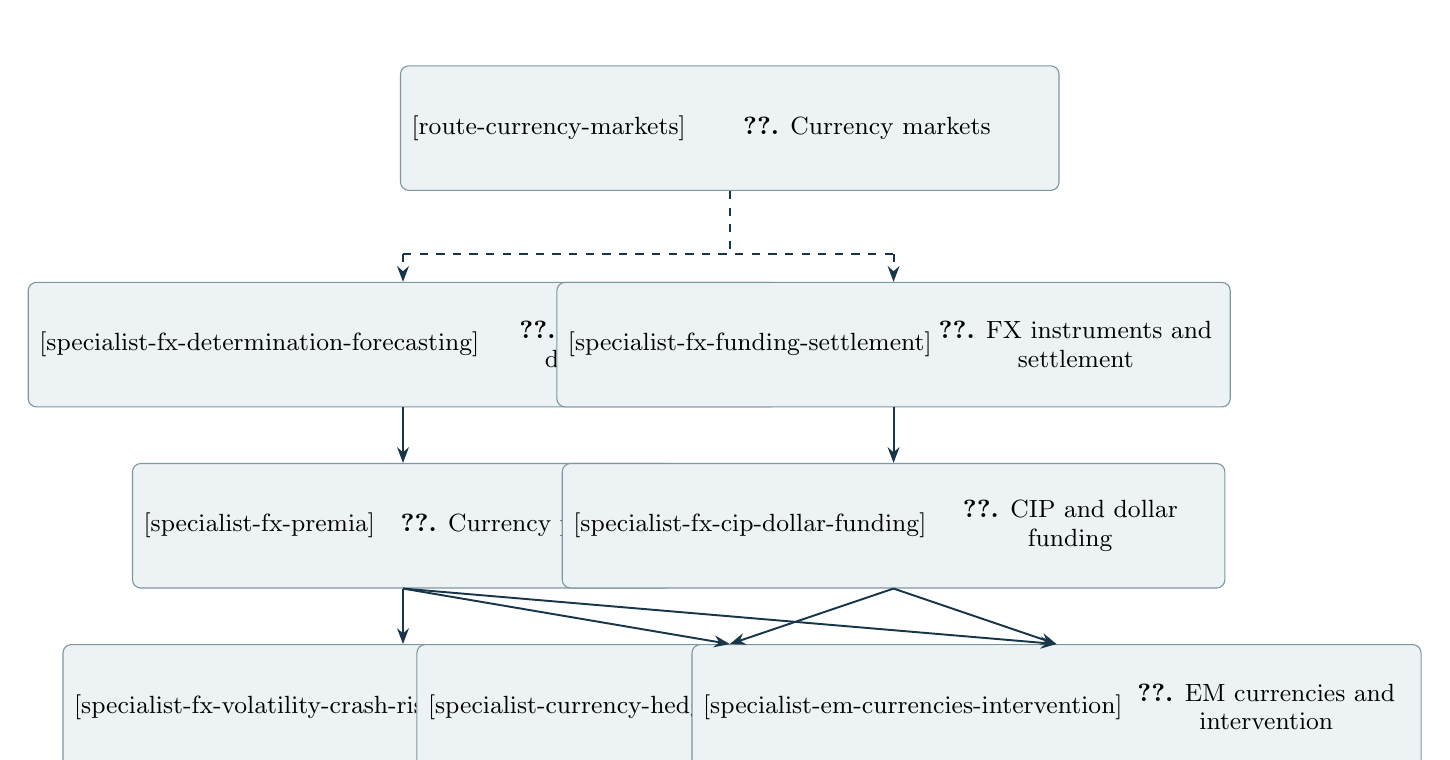
\begin{tikzpicture}[x=1cm,y=1cm]
\node[pathnode] (currency-markets) at (4.15,0) {\MeasurePathNode{4.6cm}{\textbf{\ref*{route-currency-markets}.} Currency markets}\hyperref[route-currency-markets]{\parbox[c][\pathnodeheight][c]{4.6cm}{\centering \textbf{\ref*{route-currency-markets}.} Currency markets}}};
\node[pathnode] (fx-determination-forecasting) at (0.00,-2.75) {\MeasurePathNode{3.65cm}{\textbf{\ref*{specialist-fx-determination-forecasting}.} Exchange-rate determination}\hyperref[specialist-fx-determination-forecasting]{\parbox[c][\pathnodeheight][c]{3.65cm}{\centering \textbf{\ref*{specialist-fx-determination-forecasting}.} Exchange-rate determination}}};
\node[pathnode] (fx-funding-settlement) at (6.23,-2.75) {\MeasurePathNode{3.65cm}{\textbf{\ref*{specialist-fx-funding-settlement}.} FX instruments and settlement}\hyperref[specialist-fx-funding-settlement]{\parbox[c][\pathnodeheight][c]{3.65cm}{\centering \textbf{\ref*{specialist-fx-funding-settlement}.} FX instruments and settlement}}};
\node[pathnode] (fx-premia) at (0.00,-5.05) {\MeasurePathNode{3.65cm}{\textbf{\ref*{specialist-fx-premia}.} Currency premia}\hyperref[specialist-fx-premia]{\parbox[c][\pathnodeheight][c]{3.65cm}{\centering \textbf{\ref*{specialist-fx-premia}.} Currency premia}}};
\node[pathnode] (fx-cip-dollar-funding) at (6.23,-5.05) {\MeasurePathNode{3.65cm}{\textbf{\ref*{specialist-fx-cip-dollar-funding}.} CIP and dollar funding}\hyperref[specialist-fx-cip-dollar-funding]{\parbox[c][\pathnodeheight][c]{3.65cm}{\centering \textbf{\ref*{specialist-fx-cip-dollar-funding}.} CIP and dollar funding}}};
\node[pathnode] (fx-volatility-crash-risk) at (0.00,-7.35) {\MeasurePathNode{3.65cm}{\textbf{\ref*{specialist-fx-volatility-crash-risk}.} FX volatility and crash risk}\hyperref[specialist-fx-volatility-crash-risk]{\parbox[c][\pathnodeheight][c]{3.65cm}{\centering \textbf{\ref*{specialist-fx-volatility-crash-risk}.} FX volatility and crash risk}}};
\node[pathnode] (currency-hedging) at (4.15,-7.35) {\MeasurePathNode{3.65cm}{\textbf{\ref*{specialist-currency-hedging}.} Currency hedging}\hyperref[specialist-currency-hedging]{\parbox[c][\pathnodeheight][c]{3.65cm}{\centering \textbf{\ref*{specialist-currency-hedging}.} Currency hedging}}};
\node[pathnode] (em-currencies-intervention) at (8.30,-7.35) {\MeasurePathNode{3.65cm}{\textbf{\ref*{specialist-em-currencies-intervention}.} EM currencies and intervention}\hyperref[specialist-em-currencies-intervention]{\parbox[c][\pathnodeheight][c]{3.65cm}{\centering \textbf{\ref*{specialist-em-currencies-intervention}.} EM currencies and intervention}}};
\draw[entryline] (currency-markets.south) -- (4.15,-1.60);
\draw[entryline] (0.00,-1.60) -- (6.23,-1.60);
\draw[entryarrow] (0.00,-1.60) -- (fx-determination-forecasting.north);
\draw[entryarrow] (6.23,-1.60) -- (fx-funding-settlement.north);
\draw[patharrow] (fx-determination-forecasting.south) -- (fx-premia.north);
\draw[patharrow] (fx-funding-settlement.south) -- (fx-cip-dollar-funding.north);
\draw[patharrow] (fx-premia.south) -- (fx-volatility-crash-risk.north);
\draw[patharrow] (fx-premia.south) -- (currency-hedging.north);
\draw[patharrow] (fx-cip-dollar-funding.south) -- (currency-hedging.north);
\draw[patharrow] (fx-premia.south) -- (em-currencies-intervention.north);
\draw[patharrow] (fx-cip-dollar-funding.south) -- (em-currencies-intervention.north);
\end{tikzpicture}\end{center}
\textbf{Bring these foundations with you.}\begin{itemize}
\item \hyperref[specialist-return-predictability]{Return predictability and forecast evaluation} --- needed by \hyperref[specialist-fx-determination-forecasting]{Exchange-rate determination}.
\item \hyperref[specialist-option-pricing-models]{Stochastic, local and jump volatility models} --- needed by \hyperref[specialist-fx-volatility-crash-risk]{FX volatility and crash risk}.
\end{itemize}\hyperref[learning-map]{Return to the whole-guide DAG.}
\Needspace{12\baselineskip}
\subsection{Exchange-rate determination, forecasting and order flow}\label{specialist-fx-determination-forecasting}
\textbf{Specialist pathway.} In \hyperref[route-currency-markets]{Currency markets: exchange rates, premia and hedging}.

\textbf{Outcome.} Test exchange-rate forecasts against a random walk with economic as well as statistical criteria, and explain the forward-premium puzzle, the disconnect from fundamentals and the roles of order flow and financial flows.

\textbf{Prerequisites.} Currency-markets overview; return predictability and forecast evaluation.

\textbf{Review first.} \hyperref[route-currency-markets]{Currency markets: exchange rates, premia and hedging}; \hyperref[specialist-return-predictability]{Return predictability and forecast evaluation}.

\textbf{Required readings, in order}
\begin{enumerate}\raggedright
\Needspace{5\baselineskip}\item \href{institutional_quantitative_finance_reading_list.pdf\#s16-r10}{Campbell R. Harvey, \emph{The Real Term Structure and Consumption Growth} (1988); Richard Meese and Kenneth Rogoff, \emph{Empirical Exchange Rate Models of the Seventies: Do They Fit Out of Sample?} (1983)}\CataloguePage{268}\NoteKey{s16-r10}\par \textbf{Evidence.} Start from the Meese–Rogoff finding that structural models do not beat a random walk out of sample.
\Needspace{5\baselineskip}\item \href{institutional_quantitative_finance_reading_list.pdf\#ma-engel-west-2005}{Charles Engel and Kenneth D. West, ``Exchange Rates and Fundamentals''}\CataloguePage{275}\NoteKey{ma-engel-west-2005}\par \textbf{Theory.} See why present-value models imply near–random walk exchange rates.
\Needspace{5\baselineskip}\item \href{institutional_quantitative_finance_reading_list.pdf\#ma-rossi-2013}{Barbara Rossi, ``Exchange Rate Predictability''}\CataloguePage{275}\NoteKey{ma-rossi-2013}\par \textbf{Evidence.} Survey which predictors, horizons and evaluation methods beat the random walk.
\Needspace{5\baselineskip}\item \href{institutional_quantitative_finance_reading_list.pdf\#ma-molodtsova-papell-2009}{Tanya Molodtsova and David H. Papell, ``Out-of-sample exchange rate predictability with Taylor rule fundamentals''}\CataloguePage{275}\NoteKey{ma-molodtsova-papell-2009}\par \textbf{Evidence.} Test Taylor-rule fundamentals out of sample.
\Needspace{5\baselineskip}\item \href{institutional_quantitative_finance_reading_list.pdf\#ma-della-corte-sarno-tsiakas-2009}{Pasquale Della Corte, Lucio Sarno and Ilias Tsiakas, ``An Economic Evaluation of Empirical Exchange Rate Models''}\CataloguePage{276}\NoteKey{ma-della-corte-sarno-tsiakas-2009}\par \textbf{Validation.} Value exchange-rate forecasts as a performance fee in a dynamic portfolio.
\Needspace{5\baselineskip}\item \href{institutional_quantitative_finance_reading_list.pdf\#ma-engel-wu-2023}{Charles Engel and Steve Pak Yeung Wu, ``Forecasting the U.S. Dollar in the 21st Century''}\CataloguePage{276}\NoteKey{ma-engel-wu-2023}\par \textbf{Counter-evidence.} Correct long-horizon dollar forecasts for small-sample bias.
\Needspace{5\baselineskip}\item \href{institutional_quantitative_finance_reading_list.pdf\#s16-r33}{Lars Peter Hansen and Robert J. Hodrick, \emph{Forward Exchange Rates as Optimal Predictors of Future Spot Rates: An Econometric Analysis} (1980); Eugene F. Fama, \emph{Forward and Spot Exchange Rates} (1984)}\CataloguePage{275}\NoteKey{s16-r33}\par \textbf{Evidence.} Test forward rates as predictors of future spot rates.
\Needspace{5\baselineskip}\item \href{institutional_quantitative_finance_reading_list.pdf\#ma-engel-1996}{Charles Engel, ``The forward discount anomaly and the risk premium: A survey of recent evidence''}\CataloguePage{275}\NoteKey{ma-engel-1996}\par \textbf{Evidence.} Survey the forward-discount anomaly and risk-premium models.
\Needspace{5\baselineskip}\item \href{institutional_quantitative_finance_reading_list.pdf\#cur-engel-2016}{Charles Engel, ``Exchange Rates, Interest Rates, and the Risk Premium''}\CataloguePage{277}\NoteKey{cur-engel-2016}\par \textbf{Evidence.} Set the forward-premium puzzle beside the opposite puzzle in real-rate levels that any risk-premium model must also fit.
\Needspace{5\baselineskip}\item \href{institutional_quantitative_finance_reading_list.pdf\#ma-taylor-taylor-2004}{Alan M. Taylor and Mark P. Taylor, ``The Purchasing Power Parity Debate''}\CataloguePage{276}\NoteKey{ma-taylor-taylor-2004}\par \textbf{Theory.} Judge how far purchasing power parity holds in the short and long run.
\Needspace{5\baselineskip}\item \href{institutional_quantitative_finance_reading_list.pdf\#wide-evans-lyons-orderflow}{Martin D. D. Evans and Richard K. Lyons, ``Order Flow and Exchange Rate Dynamics''}\CataloguePage{289}\NoteKey{wide-evans-lyons-orderflow}\par \textbf{Evidence.} Relate interdealer order flow to exchange-rate changes.
\Needspace{5\baselineskip}\item \href{institutional_quantitative_finance_reading_list.pdf\#w3-burnside-fx-order-flow}{Craig Burnside, Mario Cerrato and Zhekai Zhang, ``Foreign Exchange Order Flow as a Risk Factor''}\CataloguePage{290}\NoteKey{w3-burnside-fx-order-flow}\par \textbf{Evidence.} Price carry and momentum portfolios with an order-flow factor.
\Needspace{5\baselineskip}\item \href{institutional_quantitative_finance_reading_list.pdf\#cur-froot-ramadorai-2005}{Kenneth A. Froot and Tarun Ramadorai, ``Currency Returns, Intrinsic Value, and Institutional-Investor Flows''}\CataloguePage{277}\NoteKey{cur-froot-ramadorai-2005}\par \textbf{Evidence.} Separate transitory flow-driven currency returns from permanent intrinsic-value shocks.
\Needspace{5\baselineskip}\item \href{institutional_quantitative_finance_reading_list.pdf\#cur-camanho-hau-rey-2022}{Nelson Camanho, Harald Hau and H\'el\`ene Rey, ``Global Portfolio Rebalancing and Exchange Rates''}\CataloguePage{277}\NoteKey{cur-camanho-hau-rey-2022}\par \textbf{Evidence.} Trace equity-fund rebalancing flows into exchange rates and estimate a currency supply elasticity.
\Needspace{5\baselineskip}\item \href{institutional_quantitative_finance_reading_list.pdf\#ma-gabaix-maggiori-2015}{Xavier Gabaix and Matteo Maggiori, ``International Liquidity and Exchange Rate Dynamics''}\CataloguePage{276}\NoteKey{ma-gabaix-maggiori-2015}\par \textbf{Theory.} Model exchange rates set by financiers' balance sheets and capital flows.
\Needspace{5\baselineskip}\item \href{institutional_quantitative_finance_reading_list.pdf\#ma-itskhoki-mukhin-2021}{Oleg Itskhoki and Dmitry Mukhin, ``Exchange Rate Disconnect in General Equilibrium''}\CataloguePage{276}\NoteKey{ma-itskhoki-mukhin-2021}\par \textbf{Theory.} Reproduce the main exchange-rate puzzles with financial shocks in general equilibrium.
\Needspace{5\baselineskip}\item \href{institutional_quantitative_finance_reading_list.pdf\#cur-lilley-maggiori-neiman-schreger-2022}{Andrew Lilley, Matteo Maggiori, Brent Neiman and Jesse Schreger, ``Exchange Rate Reconnect''}\CataloguePage{277}\NoteKey{cur-lilley-maggiori-neiman-schreger-2022}\par \textbf{Evidence.} See risk-appetite proxies and U.S. bond purchases reconnect with the dollar after 2007, in sample.
\Needspace{5\baselineskip}\item \href{institutional_quantitative_finance_reading_list.pdf\#w3-jiang-richmond-zhang-dollar}{Zhengyang Jiang, Robert J. Richmond and Tony Zhang, ``Understanding the strength of the dollar''}\CataloguePage{279}\NoteKey{w3-jiang-richmond-zhang-dollar}\par \textbf{Evidence.} Decompose the sources of the dollar's strength.
\end{enumerate}
\Needspace{5\baselineskip}\textbf{Checkpoint.} For G10 currencies against the dollar, forecast one- and twelve-month changes in real time with uncovered-interest-parity, purchasing-power-parity, Taylor-rule and order-flow models. Compare each with a driftless random walk using Clark–West tests and the performance fee of a mean–variance investor, then repeat the twelve-month test with a small-sample bootstrap.

\textbf{Optional branches.} \href{institutional_quantitative_finance_reading_list.pdf\#ma-greenwood-hanson-stein-sunderam-2023}{Link bond supply, term premia and exchange rates.}\BranchPage{276} \href{institutional_quantitative_finance_reading_list.pdf\#ma-malamud-schrimpf-zhang-2025}{Model interest-parity deviations through intermediaries' market power.}\BranchPage{276} \href{institutional_quantitative_finance_reading_list.pdf\#exp-dao-gourinchas-itskhoki-breaking-parity}{Read a recent equilibrium view of currency premia.}\BranchPage{278} \href{institutional_quantitative_finance_reading_list.pdf\#cur-lyons-2001}{Read the microstructure approach to exchange rates in book form.}\BranchPage{277} \href{institutional_quantitative_finance_reading_list.pdf\#cur-rime-sarno-sojli-2010}{Test daily out-of-sample forecasts from order flow that aggregates macro information.}\BranchPage{277}
\par{\small \hyperref[learning-map]{Learning pathway DAG} \textbar{} \hyperref[route-currency-markets]{Section overview} \textbar{} \hyperref[map-currency-markets]{Section DAG}\NoteKey{fx-determination-forecasting}}
\Needspace{12\baselineskip}
\subsection{FX forwards, options, fixes and settlement}\label{specialist-fx-funding-settlement}
\textbf{Specialist pathway.} In \hyperref[route-currency-markets]{Currency markets: exchange rates, premia and hedging}.

\textbf{Outcome.} Price FX forwards and options with market quoting conventions, account for flows and conduct rules around benchmark fixes, measure FX liquidity, and track settlement risk to final delivery.

\textbf{Prerequisites.} Currency-markets overview; forwards, money-market discounting and option Greeks.

\textbf{Review first.} \hyperref[route-currency-markets]{Currency markets: exchange rates, premia and hedging}.

\textbf{Required readings, in order}
\begin{enumerate}\raggedright
\Needspace{5\baselineskip}\item \href{institutional_quantitative_finance_reading_list.pdf\#cur-garman-kohlhagen-1983}{Mark B. Garman and Steven W. Kohlhagen, ``Foreign currency option values''}\CataloguePage{290}\NoteKey{cur-garman-kohlhagen-1983}\par \textbf{Valuation.} Price a European currency option with domestic and foreign interest rates.
\Needspace{5\baselineskip}\item \href{institutional_quantitative_finance_reading_list.pdf\#gap-clark-fx}{Iain J. Clark, Foreign Exchange Option Pricing: A Practitioner's Guide}\CataloguePage{288}\NoteKey{gap-clark-fx}\par \textbf{Valuation.} Build option prices from FX delta and premium conventions.
\Needspace{5\baselineskip}\item \href{institutional_quantitative_finance_reading_list.pdf\#gap-fx-smile}{Dimitri Reiswich and Uwe Wystup, FX Volatility Smile Construction; Author working paper (2010 revision)}\CataloguePage{288}\NoteKey{gap-fx-smile}\par \textbf{Valuation.} Translate quoted risk reversals and butterflies into a smile.
\Needspace{5\baselineskip}\item \href{institutional_quantitative_finance_reading_list.pdf\#cur-bossens-rayee-skantzos-deelstra-2010}{Fr\'ed\'eric Bossens, Gr\'egory Ray\'ee, Nikos S. Skantzos and Griselda Deelstra, ``Vanna-Volga methods applied to FX derivatives: from theory to market practice''}\CataloguePage{290}\NoteKey{cur-bossens-rayee-skantzos-deelstra-2010}\par \textbf{Valuation.} Price first-generation exotics with the vanna--volga adjustment dealers quote from.
\Needspace{5\baselineskip}\item \href{institutional_quantitative_finance_reading_list.pdf\#exp-fx-code}{Global Foreign Exchange Committee, FX Global Code; revision and disclosure context}\CataloguePage{288}\NoteKey{exp-fx-code}\par \textbf{Mechanics.} Check execution, confirmation and settlement conduct.
\Needspace{5\baselineskip}\item \href{institutional_quantitative_finance_reading_list.pdf\#gapclose-fx-definitions-2026}{ISDA and EMTA, 2026 FX Definitions: publication and implementation; Update InfoHub}\CataloguePage{288}\NoteKey{gapclose-fx-definitions-2026}\par \textbf{Contracts.} Map the confirmation to its incorporated FX definitions and distinguish the 2026 publication from the planned 2027 transition.
\Needspace{5\baselineskip}\item \href{institutional_quantitative_finance_reading_list.pdf\#cur-fsb-fx-benchmarks-2014}{Financial Stability Board, Foreign Exchange Benchmarks: Final Report}\CataloguePage{290}\NoteKey{cur-fsb-fx-benchmarks-2014}\par \textbf{Regulation.} Learn how the WM/Reuters fix is calculated and which conduct and execution rules followed the 2013 benchmark concerns.
\Needspace{5\baselineskip}\item \href{institutional_quantitative_finance_reading_list.pdf\#cur-melvin-prins-2015}{Michael Melvin and John Prins, ``Equity hedging and exchange rates at the London 4p.m. fix''}\CataloguePage{290}\NoteKey{cur-melvin-prins-2015}\par \textbf{Evidence.} Measure how month-end equity-hedge flows executed at the London fix move exchange rates temporarily.
\Needspace{5\baselineskip}\item \href{institutional_quantitative_finance_reading_list.pdf\#cur-ito-yamada-2017}{Takatoshi Ito and Masahiro Yamada, ``Puzzles in the Tokyo fixing in the forex market: Order imbalances and Bank pricing''}\CataloguePage{290}\NoteKey{cur-ito-yamada-2017}\par \textbf{Evidence.} Compare the Tokyo fix: predictable customer imbalances and how banks set the fixing price.
\Needspace{5\baselineskip}\item \href{institutional_quantitative_finance_reading_list.pdf\#exp-fx-algos}{BIS Markets Committee, FX Execution Algorithms and Market Functioning}\CataloguePage{288}\NoteKey{exp-fx-algos}\par \textbf{Implementation.} Assess execution scheduling and market-impact evidence.
\Needspace{5\baselineskip}\item \href{institutional_quantitative_finance_reading_list.pdf\#cur-mancini-ranaldo-wrampelmeyer-2013}{Loriano Mancini, Angelo Ranaldo and Jan Wrampelmeyer, ``Liquidity in the Foreign Exchange Market: Measurement, Commonality, and Risk Premiums''}\CataloguePage{291}\NoteKey{cur-mancini-ranaldo-wrampelmeyer-2013}\par \textbf{Evidence.} Measure FX liquidity across pairs and its commonality with other markets.
\Needspace{5\baselineskip}\item \href{institutional_quantitative_finance_reading_list.pdf\#cur-karnaukh-ranaldo-soderlind-2015}{Nina Karnaukh, Angelo Ranaldo and Paul S\"oderlind, ``Understanding FX Liquidity''}\CataloguePage{291}\NoteKey{cur-karnaukh-ranaldo-soderlind-2015}\par \textbf{Data.} Build daily FX liquidity measures and see liquidity fall with funding constraints and global risk.
\Needspace{5\baselineskip}\item \href{institutional_quantitative_finance_reading_list.pdf\#cur-glowka-nilsson-2022}{Marc Glowka and Thomas Nilsson, FX settlement risk: an unsettled issue}\CataloguePage{291}\NoteKey{cur-glowka-nilsson-2022}\par \textbf{Evidence.} Size the FX turnover still settled without payment-versus-payment protection.
\Needspace{5\baselineskip}\item \href{institutional_quantitative_finance_reading_list.pdf\#cur-cpmi-pvp-2023}{Committee on Payments and Market Infrastructures, Facilitating increased adoption of payment versus payment (PvP): final report}\CataloguePage{291}\NoteKey{cur-cpmi-pvp-2023}\par \textbf{Mechanics.} Compare PvP, netting and on-us settlement and the barriers to wider PvP use.
\Needspace{5\baselineskip}\item \href{institutional_quantitative_finance_reading_list.pdf\#exp-pfmi}{CPSS and IOSCO Technical Committee, Principles for Financial Market Infrastructures}\CataloguePage{539}\NoteKey{exp-pfmi}\par \textbf{Implementation.} Trace payment and delivery finality across infrastructures.
\end{enumerate}
\Needspace{5\baselineskip}\textbf{Checkpoint.} For one currency pair, reconcile spot, both money-market curves, forward points and smile quotes at one timestamp. Price a forward and a vanilla option with premium-currency and delta conventions, and a one-touch with a vanna--volga adjustment. Identify the definitions incorporated by the confirmation and distinguish the published 2026 FX Definitions from the planned November 2027 industry transition. Measure spreads and price moves in the London 4pm fix window on month-ends, and stress an unfilled hedge and a payment that settles outside PvP, marking unavailable dealer quotes and credit limits.

\textbf{Optional branches.} \href{institutional_quantitative_finance_reading_list.pdf\#cur-castagna-fx-smile}{Read a practitioner text on FX volatility surfaces, smile risk and exotics.}\BranchPage{290} \href{institutional_quantitative_finance_reading_list.pdf\#gapclose-nigeria-ndf-rollover}{Apply the Nigeria hedge-roll case with the linked base standards, CCI conditions and unresolved amendment limits.}\BranchPage{314} \href{institutional_quantitative_finance_reading_list.pdf\#wide-wystup-fx-options}{Read a structured FX options text.}\BranchPage{289} \href{institutional_quantitative_finance_reading_list.pdf\#wide-evans-wmr-fix}{Study trading around the WMR fix.}\BranchPage{289} \href{institutional_quantitative_finance_reading_list.pdf\#ma-krohn-mueller-whelan-2024}{Trace dollar return reversals around the main FX fixes.}\BranchPage{290}
\par{\small \hyperref[learning-map]{Learning pathway DAG} \textbar{} \hyperref[route-currency-markets]{Section overview} \textbar{} \hyperref[map-currency-markets]{Section DAG}\NoteKey{fx-funding-settlement}}
\Needspace{12\baselineskip}
\subsection{Currency premia: carry, momentum, value and the dollar}\label{specialist-fx-premia}
\textbf{Specialist pathway.} In \hyperref[route-currency-markets]{Currency markets: exchange rates, premia and hedging}.

\textbf{Outcome.} Build currency carry, momentum, value and dollar portfolios, judge the risk-based and equilibrium explanations of their returns, and relate them to drawdowns, the dollar factor and the term structure of currency premia.

\textbf{Prerequisites.} Currency-markets overview; exchange-rate determination. Forward-implied returns use the conventions in FX forwards, options, fixes and settlement.

\textbf{Review first.} \hyperref[route-currency-markets]{Currency markets: exchange rates, premia and hedging}; \hyperref[specialist-fx-determination-forecasting]{Exchange-rate determination, forecasting and order flow}.

\textbf{Required readings, in order}
\begin{enumerate}\raggedright
\Needspace{5\baselineskip}\item \href{institutional_quantitative_finance_reading_list.pdf\#catalogue-0240}{Hanno Lustig, Nikolai Roussanov and Adrien Verdelhan, ``Common Risk Factors in Currency Markets''}\CataloguePage{278}\NoteKey{catalogue-0240}\par \textbf{Evidence.} Learn currency portfolio sorts and common risk factors.
\Needspace{5\baselineskip}\item \href{institutional_quantitative_finance_reading_list.pdf\#cur-lustig-verdelhan-2007}{Hanno Lustig and Adrien Verdelhan, ``The Cross Section of Foreign Currency Risk Premia and Consumption Growth Risk''}\CataloguePage{280}\NoteKey{cur-lustig-verdelhan-2007}\par \textbf{Evidence.} Price interest-rate-sorted currency portfolios with consumption growth risk.
\Needspace{5\baselineskip}\item \href{institutional_quantitative_finance_reading_list.pdf\#cur-burnside-2011}{Craig Burnside, ``The Cross Section of Foreign Currency Risk Premia and Consumption Growth Risk: Comment''}\CataloguePage{280}\NoteKey{cur-burnside-2011}\par \textbf{Counter-evidence.} Check whether that consumption model explains any of the cross-section.
\Needspace{5\baselineskip}\item \href{institutional_quantitative_finance_reading_list.pdf\#wide-menkhoff-carry}{Lukas Menkhoff, Lucio Sarno, Maik Schmeling and Andreas Schrimpf, ``Carry Trades and Global Foreign Exchange Volatility''}\CataloguePage{278}\NoteKey{wide-menkhoff-carry}\par \textbf{Evidence.} Price carry with global FX volatility.
\Needspace{5\baselineskip}\item \href{institutional_quantitative_finance_reading_list.pdf\#catalogue-0241}{Markus Brunnermeier, Stefan Nagel and Lasse Pedersen, ``Carry Trades and Currency Crashes''}\CataloguePage{278}\NoteKey{catalogue-0241}\par \textbf{Evidence.} Study carry crash risk.
\Needspace{5\baselineskip}\item \href{institutional_quantitative_finance_reading_list.pdf\#catalogue-0437}{Craig Burnside, Martin Eichenbaum, Isaac Kleshchelski and Sergio Rebelo, \emph{Do Peso Problems Explain the Returns to the Carry Trade?} (2011 journal version)}\CataloguePage{278}\NoteKey{catalogue-0437}\par \textbf{Counter-evidence.} Test whether peso problems rather than crash-risk premia explain carry returns.
\Needspace{5\baselineskip}\item \href{institutional_quantitative_finance_reading_list.pdf\#cur-daniel-hodrick-lu-2017}{Kent Daniel, Robert J. Hodrick and Zhongjin Lu, ``The Carry Trade: Risks and Drawdowns''}\CataloguePage{280}\NoteKey{cur-daniel-hodrick-lu-2017}\par \textbf{Evidence.} Compare dollar-neutral and dollar carry on skewness, downside risk and drawdowns.
\Needspace{5\baselineskip}\item \href{institutional_quantitative_finance_reading_list.pdf\#wide-menkhoff-momentum}{Lukas Menkhoff, Lucio Sarno, Maik Schmeling and Andreas Schrimpf, ``Currency momentum strategies''}\CataloguePage{278}\NoteKey{wide-menkhoff-momentum}\par \textbf{Evidence.} Assess currency momentum and its costs.
\Needspace{5\baselineskip}\item \href{institutional_quantitative_finance_reading_list.pdf\#wide-menkhoff-value}{Lukas Menkhoff, Lucio Sarno, Maik Schmeling and Andreas Schrimpf, ``Currency Value''}\CataloguePage{279}\NoteKey{wide-menkhoff-value}\par \textbf{Evidence.} Build fundamentals-adjusted value.
\Needspace{5\baselineskip}\item \href{institutional_quantitative_finance_reading_list.pdf\#cur-verdelhan-2018}{Adrien Verdelhan, ``The Share of Systematic Variation in Bilateral Exchange Rates''}\CataloguePage{280}\NoteKey{cur-verdelhan-2018}\par \textbf{Evidence.} Build the dollar factor from dollar betas and measure how much of bilateral moves it and carry explain.
\Needspace{5\baselineskip}\item \href{institutional_quantitative_finance_reading_list.pdf\#wide-lrv-countercyclical}{Hanno Lustig, Nikolai Roussanov and Adrien Verdelhan, ``Countercyclical currency risk premia''}\CataloguePage{279}\NoteKey{wide-lrv-countercyclical}\par \textbf{Evidence.} Trade the dollar countercyclically.
\Needspace{5\baselineskip}\item \href{institutional_quantitative_finance_reading_list.pdf\#cur-hassan-mano-2019}{Tarek A. Hassan and Rui C. Mano, ``Forward and Spot Exchange Rates in a Multi-Currency World''}\CataloguePage{280}\NoteKey{cur-hassan-mano-2019}\par \textbf{Evidence.} Separate the forward-premium puzzle, the dollar trade and the carry trade as distinct anomalies.
\Needspace{5\baselineskip}\item \href{institutional_quantitative_finance_reading_list.pdf\#cur-lustig-stathopoulos-verdelhan-2019}{Hanno Lustig, Andreas Stathopoulos and Adrien Verdelhan, ``The Term Structure of Currency Carry Trade Risk Premia''}\CataloguePage{280}\NoteKey{cur-lustig-stathopoulos-verdelhan-2019}\par \textbf{Evidence.} See carry premia fall with bond maturity as local term premia offset them.
\Needspace{5\baselineskip}\item \href{institutional_quantitative_finance_reading_list.pdf\#cur-backus-foresi-telmer-2001}{David K. Backus, Silverio Foresi and Chris I. Telmer, ``Affine Term Structure Models and the Forward Premium Anomaly''}\CataloguePage{280}\NoteKey{cur-backus-foresi-telmer-2001}\par \textbf{Theory.} Learn what an affine no-arbitrage model needs to generate the forward-premium anomaly.
\Needspace{5\baselineskip}\item \href{institutional_quantitative_finance_reading_list.pdf\#wide-jkl-safe-asset}{Zhengyang Jiang, Arvind Krishnamurthy and Hanno Lustig, ``Foreign Safe Asset Demand and the Dollar Exchange Rate''}\CataloguePage{279}\NoteKey{wide-jkl-safe-asset}\par \textbf{Theory.} Link the dollar to safe-asset demand.
\end{enumerate}
\Needspace{5\baselineskip}\textbf{Checkpoint.} Form G10 and EM carry, momentum, value and dollar-beta portfolios with forward-implied returns and bid--ask costs. Test whether a consumption-growth factor and the dollar and carry factors price them, reporting the Burnside-style test that the SDF explains nothing, and compare dollar-neutral with dollar carry on skewness and maximum drawdown. Then rerun the tests with a data-snooping adjustment.

\textbf{Optional branches.} \href{institutional_quantitative_finance_reading_list.pdf\#exp-dao-gourinchas-itskhoki-breaking-parity}{Read a recent equilibrium view of currency premia.}\BranchPage{278} \href{institutional_quantitative_finance_reading_list.pdf\#w3-kremens-martin-varela-fx}{Use survey FX expectations.}\BranchPage{279} \href{institutional_quantitative_finance_reading_list.pdf\#w3-hou-sarno-ye-network}{Price currencies with intermediary network centrality.}\BranchPage{279} \href{institutional_quantitative_finance_reading_list.pdf\#w4-cheemafox-greenwood-flight}{Classify crises as flights to safety or from carry using flows.}\BranchPage{279} \href{institutional_quantitative_finance_reading_list.pdf\#ma-dahlquist-hasseltoft-2020}{Trade economic momentum and see it subsume carry.}\BranchPage{274} \href{institutional_quantitative_finance_reading_list.pdf\#w4-hsu-taylor-carry-snooping}{Adjust carry strategies for data snooping and post-publication decay.}\BranchPage{279} \href{institutional_quantitative_finance_reading_list.pdf\#ma-lettau-maggiori-weber-2014}{Price carry with downside market risk across asset classes.}\BranchPage{265} \href{institutional_quantitative_finance_reading_list.pdf\#cur-farhi-gabaix-2016}{Explain currency puzzles with time-varying rare-disaster risk.}\BranchPage{281} \href{institutional_quantitative_finance_reading_list.pdf\#cur-verdelhan-2010}{Generate the UIP puzzle from habit preferences.}\BranchPage{281} \href{institutional_quantitative_finance_reading_list.pdf\#cur-colacito-croce-2011}{Explain smooth real exchange rates with correlated long-run risk.}\BranchPage{281} \href{institutional_quantitative_finance_reading_list.pdf\#cur-brandt-cochrane-santa-clara-2006}{See why smooth exchange rates imply highly correlated marginal utilities across countries.}\BranchPage{281} \href{institutional_quantitative_finance_reading_list.pdf\#cur-sandulescu-trojani-vedolin-2021}{Relate exchange rates to international SDFs when markets are incomplete or segmented.}\BranchPage{281} \href{institutional_quantitative_finance_reading_list.pdf\#cur-richmond-2019}{Explain low currency premia of countries central in the trade network.}\BranchPage{281} \href{institutional_quantitative_finance_reading_list.pdf\#cur-ready-roussanov-ward-2017}{Explain high commodity-currency interest rates and premia through trade specialisation.}\BranchPage{281}
\par{\small \hyperref[learning-map]{Learning pathway DAG} \textbar{} \hyperref[route-currency-markets]{Section overview} \textbar{} \hyperref[map-currency-markets]{Section DAG}\NoteKey{fx-premia}}
\Needspace{12\baselineskip}
\subsection{Covered interest parity, the cross-currency basis and dollar funding}\label{specialist-fx-cip-dollar-funding}
\textbf{Specialist pathway.} In \hyperref[route-currency-markets]{Currency markets: exchange rates, premia and hedging}.

\textbf{Outcome.} Measure covered-interest-parity deviations with the funding rates arbitrageurs actually face, explain the cross-currency basis through hedging demand and balance-sheet constraints, and price synthetic dollar funding across quarter-ends, crises and swap-line operations.

\textbf{Prerequisites.} FX forwards, options, fixes and settlement; money-market and OIS discounting. Funding liquidity, crowding and arbitrage capital (Part III) treats limits to arbitrage across markets.

\textbf{Review first.} \hyperref[route-currency-markets]{Currency markets: exchange rates, premia and hedging}; \hyperref[specialist-fx-funding-settlement]{FX forwards, options, fixes and settlement}.

\textbf{Required readings, in order}
\begin{enumerate}\raggedright
\Needspace{5\baselineskip}\item \href{institutional_quantitative_finance_reading_list.pdf\#cur-du-schreger-2022}{Wenxin Du and Jesse Schreger, ``CIP deviations, the dollar, and frictions in international capital markets''}\CataloguePage{282}\NoteKey{cur-du-schreger-2022}\par \textbf{Foundations.} Survey how CIP deviations are measured, what drives them and what they imply.
\Needspace{5\baselineskip}\item \href{institutional_quantitative_finance_reading_list.pdf\#cur-akram-rime-sarno-2008}{Q. Farooq Akram, Dagfinn Rime and Lucio Sarno, ``Arbitrage in the foreign exchange market: Turning on the microscope''}\CataloguePage{282}\NoteKey{cur-akram-rime-sarno-2008}\par \textbf{Evidence.} See how small and short-lived CIP arbitrage was before 2008 in tick data.
\Needspace{5\baselineskip}\item \href{institutional_quantitative_finance_reading_list.pdf\#cur-baba-packer-2009}{Naohiko Baba and Frank Packer, ``Interpreting deviations from covered interest parity during the financial market turmoil of 2007--08''}\CataloguePage{282}\NoteKey{cur-baba-packer-2009}\par \textbf{Evidence.} Link the 2007--08 euro--dollar deviations to counterparty risk and to ECB dollar auctions.
\Needspace{5\baselineskip}\item \href{institutional_quantitative_finance_reading_list.pdf\#gap-cip}{Wenxin Du, Alexander Tepper and Adrien Verdelhan, Deviations from Covered Interest Rate Parity}\CataloguePage{282}\NoteKey{gap-cip}\par \textbf{Evidence.} Document persistent post-2008 CIP deviations and their quarter-end spikes.
\Needspace{5\baselineskip}\item \href{institutional_quantitative_finance_reading_list.pdf\#cur-borio-mccauley-mcguire-sushko-2016}{Claudio Borio, Robert N. McCauley, Patrick McGuire and Vladyslav Sushko, Covered interest parity lost: understanding the cross-currency basis}\CataloguePage{282}\NoteKey{cur-borio-mccauley-mcguire-sushko-2016}\par \textbf{Mechanics.} Explain the basis by hedging demand meeting costly balance-sheet space.
\Needspace{5\baselineskip}\item \href{institutional_quantitative_finance_reading_list.pdf\#cur-rime-schrimpf-syrstad-2022}{Dagfinn Rime, Andreas Schrimpf and Olav Syrstad, ``Covered Interest Parity Arbitrage''}\CataloguePage{283}\NoteKey{cur-rime-schrimpf-syrstad-2022}\par \textbf{Evidence.} Recompute CIP with marginal funding costs and find which banks can arbitrage.
\Needspace{5\baselineskip}\item \href{institutional_quantitative_finance_reading_list.pdf\#cur-avdjiev-du-koch-shin-2019}{Stefan Avdjiev, Wenxin Du, Catherine Koch and Hyun Song Shin, ``The Dollar, Bank Leverage, and Deviations from Covered Interest Parity''}\CataloguePage{283}\NoteKey{cur-avdjiev-du-koch-shin-2019}\par \textbf{Evidence.} Relate a stronger dollar to wider deviations and lower cross-border dollar lending.
\Needspace{5\baselineskip}\item \href{institutional_quantitative_finance_reading_list.pdf\#cur-ivashina-scharfstein-stein-2015}{Victoria Ivashina, David S. Scharfstein and Jeremy C. Stein, ``Dollar Funding and the Lending Behavior of Global Banks''}\CataloguePage{283}\NoteKey{cur-ivashina-scharfstein-stein-2015}\par \textbf{Evidence.} Follow how a run on banks' wholesale dollar funding widened the basis and cut dollar lending.
\Needspace{5\baselineskip}\item \href{institutional_quantitative_finance_reading_list.pdf\#cur-abbassi-brauning-2021}{Puriya Abbassi and Falk Br\"auning, ``Demand Effects in the FX Forward Market: Micro Evidence from Banks' Dollar Hedging''}\CataloguePage{283}\NoteKey{cur-abbassi-brauning-2021}\par \textbf{Evidence.} Measure quarter-end demand effects from banks hedging dollar assets.
\Needspace{5\baselineskip}\item \href{institutional_quantitative_finance_reading_list.pdf\#cur-cenedese-della-corte-wang-2021}{Gino Cenedese, Pasquale Della Corte and Tianyu Wang, ``Currency Mispricing and Dealer Balance Sheets''}\CataloguePage{283}\NoteKey{cur-cenedese-della-corte-wang-2021}\par \textbf{Evidence.} Identify the leverage-ratio cost dealers add to synthetic dollar funding.
\Needspace{5\baselineskip}\item \href{institutional_quantitative_finance_reading_list.pdf\#cur-augustin-chernov-schmid-song-2024}{Patrick Augustin, Mikhail Chernov, Lukas Schmid and Dongho Song, ``The Term Structure of Covered Interest Rate Parity Violations''}\CataloguePage{283}\NoteKey{cur-augustin-chernov-schmid-song-2024}\par \textbf{Valuation.} Split the term structure of CIP violations into risk-based and non-risk-based constraints.
\Needspace{5\baselineskip}\item \href{institutional_quantitative_finance_reading_list.pdf\#cur-liao-2020}{Gordon Y. Liao, ``Credit migration and covered interest rate parity''}\CataloguePage{283}\NoteKey{cur-liao-2020}\par \textbf{Evidence.} See how hedged issuance links CIP deviations to cross-currency credit spreads.
\Needspace{5\baselineskip}\item \href{institutional_quantitative_finance_reading_list.pdf\#cur-du-hebert-huber-2023}{Wenxin Du, Benjamin H\'ebert and Amy Wang Huber, ``Are Intermediary Constraints Priced?''}\CataloguePage{284}\NoteKey{cur-du-hebert-huber-2023}\par \textbf{Evidence.} Price the risk that intermediary constraints tighten with a forward CIP strategy.
\Needspace{5\baselineskip}\item \href{institutional_quantitative_finance_reading_list.pdf\#cur-bahaj-reis-2022}{Saleem Bahaj and Ricardo Reis, ``Central Bank Swap Lines: Evidence on the Effects of the Lender of Last Resort''}\CataloguePage{284}\NoteKey{cur-bahaj-reis-2022}\par \textbf{Evidence.} See central-bank swap lines cap the basis and change investment flows.
\Needspace{5\baselineskip}\item \href{institutional_quantitative_finance_reading_list.pdf\#cur-borio-mccauley-mcguire-2022}{Claudio Borio, Robert N. McCauley and Patrick McGuire, Dollar debt in FX swaps and forwards: huge, missing and growing}\CataloguePage{284}\NoteKey{cur-borio-mccauley-mcguire-2022}\par \textbf{Data.} Size the off-balance-sheet dollar debt in FX swaps and forwards.
\end{enumerate}
\Needspace{5\baselineskip}\textbf{Checkpoint.} For EUR, JPY and CHF against USD, compute daily three-month and five-year cross-currency bases from overnight-index-swap and RFR curves and from forward points. Mark quarter- and year-end windows, overlay Federal Reserve swap-line usage and the broad dollar index, and decompose a Japanese investor's hedged Treasury yield into the rate differential and the basis. Recompute the three-month basis with the funding rates of a high-rated and a lower-rated bank, and report which arbitrage survives balance-sheet costs.

\textbf{Optional branches.} \href{institutional_quantitative_finance_reading_list.pdf\#cur-syrstad-viswanath-natraj-2022}{Measure the price impact of FX swap order flow around quarter-ends and policy announcements.}\BranchPage{284} \href{institutional_quantitative_finance_reading_list.pdf\#cur-cerutti-obstfeld-zhou-2021}{Relate the basis to FX liquidity, intermediary risk capacity, policy and year-end effects.}\BranchPage{284} \href{institutional_quantitative_finance_reading_list.pdf\#w3-anderson-du-schlusche-arbitrage}{See how global banks allocate arbitrage capital across CIP and other trades.}\BranchPage{282} \href{institutional_quantitative_finance_reading_list.pdf\#w3-kloks-segmented-dollar}{Explain CIP with segmented dollar funding.}\BranchPage{282} \href{institutional_quantitative_finance_reading_list.pdf\#rt-du-im-schreger-2018}{Compare the CIP basis with the U.S. Treasury premium.}\BranchPage{223} \href{institutional_quantitative_finance_reading_list.pdf\#w4-ding-rutkowski-ccbs}{Value cross-currency basis swaps that reference backward-looking rates.}\BranchPage{225} \href{institutional_quantitative_finance_reading_list.pdf\#ma-malamud-schrimpf-zhang-2025}{Model interest-parity deviations through intermediaries' market power.}\BranchPage{276} \href{institutional_quantitative_finance_reading_list.pdf\#section.13.6}{Browse the covered-interest-parity and dollar-funding section.}\BranchPage{282}
\par{\small \hyperref[learning-map]{Learning pathway DAG} \textbar{} \hyperref[route-currency-markets]{Section overview} \textbar{} \hyperref[map-currency-markets]{Section DAG}\NoteKey{fx-cip-dollar-funding}}
\Needspace{12\baselineskip}
\subsection{FX volatility, skew and crash risk}\label{specialist-fx-volatility-crash-risk}
\textbf{Specialist pathway.} In \hyperref[route-currency-markets]{Currency markets: exchange rates, premia and hedging}.

\textbf{Outcome.} Read currency risk-neutral distributions from quoted smiles, separate crash, volatility and correlation risk premia from carry returns, and test whether option-implied measures forecast currencies.

\textbf{Prerequisites.} Currency premia; the smile quotation conventions in FX forwards, options, fixes and settlement; stochastic, local and jump volatility models.

\textbf{Review first.} \hyperref[route-currency-markets]{Currency markets: exchange rates, premia and hedging}; \hyperref[specialist-option-pricing-models]{Stochastic, local and jump volatility models}; \hyperref[specialist-fx-premia]{Currency premia: carry, momentum, value and the dollar}.

\textbf{Required readings, in order}
\begin{enumerate}\raggedright
\Needspace{5\baselineskip}\item \href{institutional_quantitative_finance_reading_list.pdf\#wide-bates-svj}{David S. Bates, ``Jumps and Stochastic Volatility: Exchange Rate Processes Implicit in Deutsche Mark Options''}\CataloguePage{119}\NoteKey{wide-bates-svj}\par \textbf{Evidence.} Read jump and stochastic-volatility risk from Deutsche mark options.
\Needspace{5\baselineskip}\item \href{institutional_quantitative_finance_reading_list.pdf\#cur-carr-wu-2007}{Peter Carr and Liuren Wu, ``Stochastic skew in currency options''}\CataloguePage{285}\NoteKey{cur-carr-wu-2007}\par \textbf{Valuation.} Model a currency skew that varies over time and changes sign.
\Needspace{5\baselineskip}\item \href{institutional_quantitative_finance_reading_list.pdf\#cur-bakshi-carr-wu-2008}{Gurdip Bakshi, Peter Carr and Liuren Wu, ``Stochastic risk premiums, stochastic skewness in currency options, and stochastic discount factors in international economies''}\CataloguePage{285}\NoteKey{cur-bakshi-carr-wu-2008}\par \textbf{Theory.} Infer country and global risk premia and priced downside jumps from a currency-option triangle.
\Needspace{5\baselineskip}\item \href{institutional_quantitative_finance_reading_list.pdf\#cur-della-corte-sarno-tsiakas-2011}{Pasquale Della Corte, Lucio Sarno and Ilias Tsiakas, ``Spot and forward volatility in foreign exchange''}\CataloguePage{285}\NoteKey{cur-della-corte-sarno-tsiakas-2011}\par \textbf{Evidence.} Test forward volatility agreements and find volatility term premiums.
\Needspace{5\baselineskip}\item \href{institutional_quantitative_finance_reading_list.pdf\#wide-della-corte-vrp-fx}{Pasquale Della Corte, Tarun Ramadorai and Lucio Sarno, ``Volatility risk premia and exchange rate predictability''}\CataloguePage{284}\NoteKey{wide-della-corte-vrp-fx}\par \textbf{Evidence.} Use FX volatility risk premia to predict currency returns.
\Needspace{5\baselineskip}\item \href{institutional_quantitative_finance_reading_list.pdf\#cur-londono-zhou-2017}{Juan M. Londono and Hao Zhou, ``Variance risk premiums and the forward premium puzzle''}\CataloguePage{285}\NoteKey{cur-londono-zhou-2017}\par \textbf{Evidence.} Separate the currency variance risk premium from the equity one as predictors.
\Needspace{5\baselineskip}\item \href{institutional_quantitative_finance_reading_list.pdf\#cur-jurek-2014}{Jakub W. Jurek, ``Crash-neutral currency carry trades''}\CataloguePage{285}\NoteKey{cur-jurek-2014}\par \textbf{Evidence.} Hedge carry with out-of-the-money options and measure how much return is crash premium.
\Needspace{5\baselineskip}\item \href{institutional_quantitative_finance_reading_list.pdf\#cur-farhi-et-al-2009}{Emmanuel Farhi, Samuel P. Fraiberger, Xavier Gabaix, Romain Ranciere and Adrien Verdelhan, ``Crash Risk in Currency Markets''}\CataloguePage{285}\NoteKey{cur-farhi-et-al-2009}\par \textbf{Evidence.} Estimate a world disaster-risk premium from spot, forward and option data.
\Needspace{5\baselineskip}\item \href{institutional_quantitative_finance_reading_list.pdf\#cur-chernov-graveline-zviadadze-2018}{Mikhail Chernov, Jeremy Graveline and Irina Zviadadze, ``Crash Risk in Currency Returns''}\CataloguePage{285}\NoteKey{cur-chernov-graveline-zviadadze-2018}\par \textbf{Evidence.} Estimate jumps in exchange rates and in their variance and their link to announcements.
\Needspace{5\baselineskip}\item \href{institutional_quantitative_finance_reading_list.pdf\#cur-caballero-doyle-2012}{Ricardo J. Caballero and Joseph B. Doyle, ``Carry Trade and Systemic Risk: Why are FX Options so Cheap?''}\CataloguePage{285}\NoteKey{cur-caballero-doyle-2012}\par \textbf{Counter-evidence.} Test the claim that FX options are cheap systemic insurance for carry.
\Needspace{5\baselineskip}\item \href{institutional_quantitative_finance_reading_list.pdf\#w3-li-sarno-zinna-skewness}{Junye Li, Lucio Sarno and Gabriele Zinna, ``Skewness Risk Premia and the Cross Section of Currency Returns''}\CataloguePage{284}\NoteKey{w3-li-sarno-zinna-skewness}\par \textbf{Evidence.} Trade currency skewness risk premia.
\Needspace{5\baselineskip}\item \href{institutional_quantitative_finance_reading_list.pdf\#cur-fan-londono-xiao-2022}{Zhenzhen Fan, Juan M. Londono and Xiao Xiao, ``Equity tail risk and currency risk premiums''}\CataloguePage{286}\NoteKey{cur-fan-londono-xiao-2022}\par \textbf{Evidence.} Price currencies with an option-based equity tail-risk factor.
\Needspace{5\baselineskip}\item \href{institutional_quantitative_finance_reading_list.pdf\#cur-mueller-stathopoulos-vedolin-2017}{Philippe Mueller, Andreas Stathopoulos and Andrea Vedolin, ``International correlation risk''}\CataloguePage{286}\NoteKey{cur-mueller-stathopoulos-vedolin-2017}\par \textbf{Evidence.} Price FX correlation dispersion in spot and option markets.
\Needspace{5\baselineskip}\item \href{institutional_quantitative_finance_reading_list.pdf\#cur-kremens-martin-2019}{Lukas Kremens and Ian Martin, ``The Quanto Theory of Exchange Rates''}\CataloguePage{286}\NoteKey{cur-kremens-martin-2019}\par \textbf{Evidence.} Forecast currency appreciation from quanto-implied risk-neutral covariances.
\end{enumerate}
\Needspace{5\baselineskip}\textbf{Checkpoint.} For EUR/USD, USD/JPY and AUD/USD, build daily risk-neutral densities from one-month at-the-money, 25-delta risk-reversal and butterfly quotes, and compute implied variance, skewness and the variance risk premium. Compare carry returns with and without 10-delta option protection through 2008, the January 2015 Swiss franc move and August 2024, and test whether risk reversals and the variance risk premium forecast one-month currency excess returns out of sample.

\textbf{Optional branches.} \href{institutional_quantitative_finance_reading_list.pdf\#cur-beber-breedon-buraschi-2010}{Relate forecaster disagreement to implied volatility, the smile and currency returns.}\BranchPage{286} \href{institutional_quantitative_finance_reading_list.pdf\#cur-farhi-gabaix-2016}{See the disaster-risk model behind option-implied crash premia.}\BranchPage{281} \href{institutional_quantitative_finance_reading_list.pdf\#exp-bis-august-2024-carry-unwind}{Study the August 2024 yen carry unwind as a crash episode.}\BranchPage{179} \href{institutional_quantitative_finance_reading_list.pdf\#section.13.7}{Browse the FX volatility and crash-risk section.}\BranchPage{284}
\par{\small \hyperref[learning-map]{Learning pathway DAG} \textbar{} \hyperref[route-currency-markets]{Section overview} \textbar{} \hyperref[map-currency-markets]{Section DAG}\NoteKey{fx-volatility-crash-risk}}
\Needspace{12\baselineskip}
\subsection{Currency hedging for international portfolios}\label{specialist-currency-hedging}
\textbf{Specialist pathway.} In \hyperref[route-currency-markets]{Currency markets: exchange rates, premia and hedging}.

\textbf{Outcome.} Choose and justify a currency-hedge ratio for international equity and bond portfolios, allowing for currency–equity correlations, horizon, hedging costs through the cross-currency basis and active management of the currency exposure.

\textbf{Prerequisites.} Currency premia; covered interest parity, the cross-currency basis and dollar funding.

\textbf{Review first.} \hyperref[route-currency-markets]{Currency markets: exchange rates, premia and hedging}; \hyperref[specialist-fx-premia]{Currency premia: carry, momentum, value and the dollar}; \hyperref[specialist-fx-cip-dollar-funding]{Covered interest parity, the cross-currency basis and dollar funding}.

\textbf{Required readings, in order}
\begin{enumerate}\raggedright
\Needspace{5\baselineskip}\item \href{institutional_quantitative_finance_reading_list.pdf\#ma-black-1989}{Fischer Black, ``Universal Hedging: Optimizing Currency Risk and Reward in International Equity Portfolios''}\CataloguePage{286}\NoteKey{ma-black-1989}\par \textbf{Theory.} Derive the universal hedge ratio and its assumptions.
\Needspace{5\baselineskip}\item \href{institutional_quantitative_finance_reading_list.pdf\#ma-froot-1993}{Kenneth Froot, ``Currency Hedging over Long Horizons''}\CataloguePage{286}\NoteKey{ma-froot-1993}\par \textbf{Evidence.} See why full hedging lowers variance at short but not long horizons.
\Needspace{5\baselineskip}\item \href{institutional_quantitative_finance_reading_list.pdf\#ma-campbell-serfaty-de-medeiros-viceira-2010}{John Y. Campbell, Karine Serfaty-de Medeiros and Luis M. Viceira, ``Global Currency Hedging''}\CataloguePage{286}\NoteKey{ma-campbell-serfaty-de-medeiros-viceira-2010}\par \textbf{Evidence.} Find which currencies hedge world equity risk and why bond investors hedge almost fully.
\Needspace{5\baselineskip}\item \href{institutional_quantitative_finance_reading_list.pdf\#w4-viceira-shen-currency-exposure}{Luis M. Viceira and Sally Shen, ``Optimal Currency Exposure When Interest Parity Fails''}\CataloguePage{287}\NoteKey{w4-viceira-shen-currency-exposure}\par \textbf{Theory.} Set currency exposure when interest parity fails.
\Needspace{5\baselineskip}\item \href{institutional_quantitative_finance_reading_list.pdf\#ma-kroencke-schindler-schrimpf-2014}{Tim A. Kroencke, Felix Schindler and Andreas Schrimpf, ``International Diversification Benefits with Foreign Exchange Investment Styles''}\CataloguePage{287}\NoteKey{ma-kroencke-schindler-schrimpf-2014}\par \textbf{Evidence.} Add carry, momentum and value currency styles to international portfolios.
\Needspace{5\baselineskip}\item \href{institutional_quantitative_finance_reading_list.pdf\#ma-opie-riddiough-2020}{Wei Opie and Steven J. Riddiough, ``Global currency hedging with common risk factors''}\CataloguePage{287}\NoteKey{ma-opie-riddiough-2020}\par \textbf{Implementation.} Hedge dynamically using predictable currency returns.
\Needspace{5\baselineskip}\item \href{institutional_quantitative_finance_reading_list.pdf\#w4-castro-harvey-fx-hedging}{Pedro Castro, Carl Hamill, John Harber, Campbell R. Harvey and Otto Van Hemert, ``The Best Strategies for FX Hedging''}\CataloguePage{287}\NoteKey{w4-castro-harvey-fx-hedging}\par \textbf{Implementation.} Condition hedge ratios on carry, trend and value.
\Needspace{5\baselineskip}\item \href{institutional_quantitative_finance_reading_list.pdf\#ma-sialm-zhu-2024}{Clemens Sialm and Qifei Zhu, ``Currency Management by International Fixed-Income Mutual Funds''}\CataloguePage{287}\NoteKey{ma-sialm-zhu-2024}\par \textbf{Evidence.} See how much international bond funds hedge and why.
\Needspace{5\baselineskip}\item \href{institutional_quantitative_finance_reading_list.pdf\#gap-dollar-hedging}{Wenxin Du and Amy W. Huber, Dollar Asset Holdings and Hedging around the Globe; Earlier NBER working paper}\CataloguePage{288}\NoteKey{gap-dollar-hedging}\par \textbf{Evidence.} Connect hedging demand to the dollar basis and bond investment.
\Needspace{5\baselineskip}\item \href{institutional_quantitative_finance_reading_list.pdf\#ma-liao-zhang-2025}{Gordon Y. Liao and Tony Zhang, ``The Hedging Channel of Exchange Rate Determination''}\CataloguePage{287}\NoteKey{ma-liao-zhang-2025}\par \textbf{Theory.} Link hedging demand in distress to spot and forward exchange rates.
\Needspace{5\baselineskip}\item \href{institutional_quantitative_finance_reading_list.pdf\#w3-aldunate-pension-cip}{Felipe Aldunate, Zhi Da, Borja Larrain and Clemens Sialm, ``Pension fund flows, exchange rates, and covered interest rate parity''}\CataloguePage{279}\NoteKey{w3-aldunate-pension-cip}\par \textbf{Evidence.} Trace pension-fund hedging flows to exchange rates and CIP deviations.
\Needspace{5\baselineskip}\item \href{institutional_quantitative_finance_reading_list.pdf\#w4-opie-riddiough-dollar-insurance}{Wei Opie and Steven J. Riddiough, ``The End of Crisis Insurance? Reassessing the US Dollar and the Case for Currency Hedging''}\CataloguePage{287}\NoteKey{w4-opie-riddiough-dollar-insurance}\par \textbf{Counter-evidence.} Stress hedge ratios if the dollar stops acting as crisis insurance.
\end{enumerate}
\Needspace{5\baselineskip}\textbf{Checkpoint.} For a euro-, yen- or sterling-based investor holding world equities and global bonds, compare unhedged, fully hedged, universal and minimum-variance hedge ratios over one-month and five-year horizons. Include forward-implied hedging costs with the cross-currency basis, add a dynamic hedge conditioned on carry and momentum, and report how each choice behaved in 2008, 2020 and 2022.

\textbf{Optional branches.} \href{institutional_quantitative_finance_reading_list.pdf\#w4-cheemafox-greenwood-flight}{Classify crises as flights to safety or from carry using flows.}\BranchPage{279} \href{institutional_quantitative_finance_reading_list.pdf\#ma-ang-bekaert-2002}{Value currency hedging when international correlations switch regime.}\BranchPage{269} \href{institutional_quantitative_finance_reading_list.pdf\#cur-ranaldo-soderlind-2010}{Check which currencies have hedged equity sell-offs, from hours to days.}\BranchPage{281} \href{institutional_quantitative_finance_reading_list.pdf\#section.13.8}{Browse the currency-hedging section.}\BranchPage{286}
\par{\small \hyperref[learning-map]{Learning pathway DAG} \textbar{} \hyperref[route-currency-markets]{Section overview} \textbar{} \hyperref[map-currency-markets]{Section DAG}\NoteKey{currency-hedging}}
\Needspace{12\baselineskip}
\subsection{Emerging-market currencies: regimes, intervention and the global financial cycle}\label{specialist-em-currencies-intervention}
\textbf{Specialist pathway.} In \hyperref[route-currency-markets]{Currency markets: exchange rates, premia and hedging}.

\textbf{Outcome.} Classify de facto exchange-rate regimes, judge the credibility of pegs, floors and target zones from option prices, assess FX intervention and crisis indicators, and stress emerging-market currency positions for dollar and global-financial-cycle shocks and NDF segmentation.

\textbf{Prerequisites.} Currency premia, which builds on exchange-rate determination; covered interest parity and dollar funding. Sovereign default, restructuring and local-currency debt (section 6) covers local-currency sovereign risk; global and regional markets (section 15) covers capital flows, local-currency bonds and country market access.

\textbf{Review first.} \hyperref[route-currency-markets]{Currency markets: exchange rates, premia and hedging}; \hyperref[specialist-fx-premia]{Currency premia: carry, momentum, value and the dollar}; \hyperref[specialist-fx-cip-dollar-funding]{Covered interest parity, the cross-currency basis and dollar funding}.

\textbf{Required readings, in order}
\begin{enumerate}\raggedright
\Needspace{5\baselineskip}\item \href{institutional_quantitative_finance_reading_list.pdf\#cur-ilzetzki-reinhart-rogoff-2019}{Ethan Ilzetzki, Carmen M. Reinhart and Kenneth S. Rogoff, ``Exchange Arrangements Entering the Twenty-First Century: Which Anchor will Hold?''}\CataloguePage{291}\NoteKey{cur-ilzetzki-reinhart-rogoff-2019}\par \textbf{Data.} Classify de facto regimes and anchor currencies rather than trusting declared regimes.
\Needspace{5\baselineskip}\item \href{institutional_quantitative_finance_reading_list.pdf\#cur-calvo-reinhart-2002}{Guillermo A. Calvo and Carmen M. Reinhart, ``Fear of Floating''}\CataloguePage{292}\NoteKey{cur-calvo-reinhart-2002}\par \textbf{Evidence.} See why most declared floats are managed.
\Needspace{5\baselineskip}\item \href{institutional_quantitative_finance_reading_list.pdf\#cur-krugman-1991}{Paul R. Krugman, ``Target Zones and Exchange Rate Dynamics''}\CataloguePage{292}\NoteKey{cur-krugman-1991}\par \textbf{Theory.} Model a currency inside a target zone as an option-like problem.
\Needspace{5\baselineskip}\item \href{institutional_quantitative_finance_reading_list.pdf\#cur-jermann-2017}{Urban J. Jermann, ``Financial Markets' Views about the Euro--Swiss Franc Floor''}\CataloguePage{292}\NoteKey{cur-jermann-2017}\par \textbf{Valuation.} Back out a floor's credibility from euro--Swiss franc option prices.
\Needspace{5\baselineskip}\item \href{institutional_quantitative_finance_reading_list.pdf\#cur-krugman-1979}{Paul Krugman, ``A Model of Balance-of-Payments Crises''}\CataloguePage{292}\NoteKey{cur-krugman-1979}\par \textbf{Theory.} Learn the first-generation speculative-attack model of a peg.
\Needspace{5\baselineskip}\item \href{institutional_quantitative_finance_reading_list.pdf\#cur-kaminsky-reinhart-1999}{Graciela L. Kaminsky and Carmen M. Reinhart, ``The Twin Crises: The Causes of Banking and Balance-of-Payments Problems''}\CataloguePage{292}\NoteKey{cur-kaminsky-reinhart-1999}\par \textbf{Evidence.} Trace how banking and currency crises reinforce each other.
\Needspace{5\baselineskip}\item \href{institutional_quantitative_finance_reading_list.pdf\#cur-sarno-taylor-2001}{Lucio Sarno and Mark P. Taylor, ``Official Intervention in the Foreign Exchange Market: Is It Effective and, If So, How Does It Work?''}\CataloguePage{292}\NoteKey{cur-sarno-taylor-2001}\par \textbf{Evidence.} Review when and through which channels intervention works.
\Needspace{5\baselineskip}\item \href{institutional_quantitative_finance_reading_list.pdf\#cur-fratzscher-et-al-2019}{Marcel Fratzscher, Oliver Gloede, Lukas Menkhoff, Lucio Sarno and Tobias St\"ohr, ``When Is Foreign Exchange Intervention Effective? Evidence from 33 Countries''}\CataloguePage{293}\NoteKey{cur-fratzscher-et-al-2019}\par \textbf{Evidence.} Measure intervention success across 33 countries and regimes.
\Needspace{5\baselineskip}\item \href{institutional_quantitative_finance_reading_list.pdf\#cur-adler-chang-mano-shao-2025}{Gustavo Adler, Kyun Suk Chang, Rui C. Mano and Yuting Shao, ``Foreign Exchange Intervention: A Data Set of Official Data and Estimates''}\CataloguePage{293}\NoteKey{cur-adler-chang-mano-shao-2025}\par \textbf{Data.} Use official and estimated intervention series and know which is which.
\Needspace{5\baselineskip}\item \href{institutional_quantitative_finance_reading_list.pdf\#cur-miranda-agrippino-rey-2020}{Silvia Miranda-Agrippino and H\'el\`ene Rey, ``U.S. Monetary Policy and the Global Financial Cycle''}\CataloguePage{293}\NoteKey{cur-miranda-agrippino-rey-2020}\par \textbf{Evidence.} Trace U.S. monetary shocks through the global financial cycle to floating-rate countries.
\Needspace{5\baselineskip}\item \href{institutional_quantitative_finance_reading_list.pdf\#cur-avdjiev-bruno-koch-shin-2019}{Stefan Avdjiev, Valentina Bruno, Catherine Koch and Hyun Song Shin, ``The Dollar Exchange Rate as a Global Risk Factor: Evidence from Investment''}\CataloguePage{293}\NoteKey{cur-avdjiev-bruno-koch-shin-2019}\par \textbf{Evidence.} Treat dollar strength as a financial shock to emerging-market investment.
\Needspace{5\baselineskip}\item \href{institutional_quantitative_finance_reading_list.pdf\#rt-hss-em-premia-2020}{Boris Hofmann, Ilhyock Shim and Hyun Song Shin, ``Bond Risk Premia and The Exchange Rate''}\CataloguePage{231}\NoteKey{rt-hss-em-premia-2020}\par \textbf{Evidence.} Relate local-currency bond risk premia to the exchange rate.
\Needspace{5\baselineskip}\item \href{institutional_quantitative_finance_reading_list.pdf\#cur-mccauley-shu-ma-2014}{Robert McCauley, Chang Shu and Guonan Ma, Non-deliverable forwards: 2013 and beyond}\CataloguePage{294}\NoteKey{cur-mccauley-shu-ma-2014}\par \textbf{Mechanics.} Learn how NDFs settle, who uses them and how they price against onshore forwards.
\Needspace{5\baselineskip}\item \href{institutional_quantitative_finance_reading_list.pdf\#gap-eme-fx}{Philip Wooldridge, Renminbi propels the growth of EME currency trading}\CataloguePage{289}\NoteKey{gap-eme-fx}\par \textbf{Mechanics.} Separate onshore, offshore and NDF trading in emerging-market currencies.
\Needspace{5\baselineskip}\item \href{institutional_quantitative_finance_reading_list.pdf\#cur-dao-gourinchas-2026}{Mai Chi Dao and Pierre-Olivier Gourinchas, ``Covered interest parity in emerging markets: Measurement and drivers''}\CataloguePage{294}\NoteKey{cur-dao-gourinchas-2026}\par \textbf{Evidence.} Measure an emerging-market CIP basis free of local credit risk.
\end{enumerate}
\Needspace{5\baselineskip}\textbf{Checkpoint.} For five emerging-market currencies, for example BRL, INR, KRW, TRY and ZAR, classify the 2000--2025 regimes with the Ilzetzki--Reinhart--Rogoff codes, line up IMF intervention series and capital-flow measures, and compare onshore-forward, NDF and purified CIP bases. Estimate each currency's beta to the broad dollar and to a global-financial-cycle factor, test whether announced intervention dampens moves in stress windows, and back out the implied survival probability of one peg or floor from option prices. State which official series are estimates rather than reported data.

\textbf{Optional branches.} \href{institutional_quantitative_finance_reading_list.pdf\#cur-ilzetzki-reinhart-rogoff-2022}{Follow the classification forward: reserves replacing capital controls, the Triffin dilemma and the renminbi.}\BranchPage{291} \href{institutional_quantitative_finance_reading_list.pdf\#cur-obstfeld-1996}{Model self-fulfilling currency crises with multiple equilibria.}\BranchPage{292} \href{institutional_quantitative_finance_reading_list.pdf\#cur-frankel-rose-1996}{Estimate currency-crash probabilities from macro and debt-composition indicators.}\BranchPage{292} \href{institutional_quantitative_finance_reading_list.pdf\#cur-menkhoff-2013}{Survey how emerging-market intervention differs from advanced-economy intervention.}\BranchPage{293} \href{institutional_quantitative_finance_reading_list.pdf\#cur-rey-2015}{Read the dilemma-not-trilemma argument for capital-flow policy.}\BranchPage{293} \href{institutional_quantitative_finance_reading_list.pdf\#cur-bruno-shin-2015}{Model bank leverage transmitting global liquidity across borders.}\BranchPage{293} \href{institutional_quantitative_finance_reading_list.pdf\#cur-forbes-fratzscher-straub-2015}{Check what capital-flow management measures do and do not achieve.}\BranchPage{293} \href{institutional_quantitative_finance_reading_list.pdf\#cur-cheung-rime-2014}{Study offshore renminbi order flow and its lead over the onshore rate.}\BranchPage{294} \href{institutional_quantitative_finance_reading_list.pdf\#cur-gopinath-et-al-2020}{See why dollar invoicing makes the dollar rate dominate trade pass-through.}\BranchPage{294} \href{institutional_quantitative_finance_reading_list.pdf\#cur-maggiori-neiman-schreger-2020}{Measure currency bias in global portfolios and the post-2008 dollar shift.}\BranchPage{294} \href{institutional_quantitative_finance_reading_list.pdf\#cur-jiang-krishnamurthy-lustig-2024}{Model the global financial cycle as a dollar cycle driven by safe-asset demand.}\BranchPage{294} \href{institutional_quantitative_finance_reading_list.pdf\#depth-africa-jse-hedges}{Compare South African currency futures with exchange-control rules for authorised dealers.}\BranchPage{313} \href{institutional_quantitative_finance_reading_list.pdf\#depth-latam-idb-flows}{See how foreign holdings affect Latin American local-currency bond markets.}\BranchPage{308}
\par{\small \hyperref[learning-map]{Learning pathway DAG} \textbar{} \hyperref[route-currency-markets]{Section overview} \textbar{} \hyperref[map-currency-markets]{Section DAG}\NoteKey{em-currencies-intervention}}
\clearpage
\section{International and emerging equity markets}\label{route-international-equity-markets}
\label{route-27}
\textbf{Learning sequence.} Start with integration, diversification and home bias. Global factors, emerging and frontier markets, and cross-listings build on it, and the China pathway draws on global factors and emerging-market evidence. Capital flows, local-currency bonds and market access follow in the next section.

\textbf{Section goals.} Across its pathways, this section teaches you to:
\begin{itemize}[leftmargin=1.4em,itemsep=0pt,topsep=1pt]
\item price assets under integration and segmentation, measure integration and explain home bias (\hyperref[specialist-intl-equity-integration]{\ref*{specialist-intl-equity-integration}})
\item test factors and country-selection signals across countries (\hyperref[specialist-global-equity-factors]{\ref*{specialist-global-equity-factors}})
\item adapt equity research to emerging and frontier markets (\hyperref[specialist-em-frontier-equities]{\ref*{specialist-em-frontier-equities}})
\item trade cross-listed and asynchronously priced securities (\hyperref[specialist-cross-listing-global-trading]{\ref*{specialist-cross-listing-global-trading}})
\item adapt factor and machine-learning research to China's stock market and its access channels (\hyperref[specialist-china-em-equities]{\ref*{specialist-china-em-equities}})
\end{itemize}
\textbf{Overview outcome.} Measure equity-market integration and diversification gains across developed, emerging and frontier markets without relying on raw correlations, in local currency and in dollars, hedged and unhedged, after survivorship, reclassification and stale-price corrections.

\textbf{Prerequisites.} Systematic equities; currency translation and forward hedging from the Currency markets overview. Currency hedging for international portfolios (13.6) helps.

\textbf{Review first.} \hyperref[route-systematic-equities]{Systematic equities}; \hyperref[route-currency-markets]{Currency markets: exchange rates, premia and hedging}.

\textbf{Required readings, in order}
\begin{enumerate}\raggedright
\Needspace{5\baselineskip}\item \href{institutional_quantitative_finance_reading_list.pdf\#gr-karolyi-stulz-2003}{G. Andrew Karolyi and Ren\'e M. Stulz, ``Are financial assets priced locally or globally?''}\CataloguePage{295}\NoteKey{gr-karolyi-stulz-2003}\par Start with the survey of whether risk premia are set by world or local factors, and why holdings, flows and correlations defeat the simplest global models.
\Needspace{5\baselineskip}\item \href{institutional_quantitative_finance_reading_list.pdf\#gr-jorion-goetzmann-1999}{Philippe Jorion and William N. Goetzmann, ``Global Stock Markets in the Twentieth Century''}\CataloguePage{297}\NoteKey{gr-jorion-goetzmann-1999}\par Use the 39-market record to see why US equity history is a survivor, not a base rate.
\Needspace{5\baselineskip}\item \href{institutional_quantitative_finance_reading_list.pdf\#gr-coeurdacier-rey-2013}{Nicolas Coeurdacier and H\'el\`ene Rey, ``Home Bias in Open Economy Financial Macroeconomics''}\CataloguePage{295}\NoteKey{gr-coeurdacier-rey-2013}\par Organise the explanations of home bias: hedging motives, trade costs and information frictions.
\Needspace{5\baselineskip}\item \href{institutional_quantitative_finance_reading_list.pdf\#gr-bekaert-harvey-2003}{Geert Bekaert and Campbell R. Harvey, ``Emerging markets finance''}\CataloguePage{303}\NoteKey{gr-bekaert-harvey-2003}\par Separate liberalisation from integration and survey what is distinctive about emerging-market finance.
\Needspace{5\baselineskip}\item \href{institutional_quantitative_finance_reading_list.pdf\#gr-carpenter-whitelaw-2017}{Jennifer N. Carpenter and Robert F. Whitelaw, ``The Development of China's Stock Market and Stakes for the Global Economy''}\CataloguePage{316}\NoteKey{gr-carpenter-whitelaw-2017}\par Learn the institutions and research on China's stock market before applying US paradigms.
\end{enumerate}
\Needspace{5\baselineskip}\textbf{Checkpoint, a section capstone: complete it after \hyperref[specialist-intl-equity-integration]{\ref*{specialist-intl-equity-integration}}.} Build a monthly panel of MSCI or FTSE country equity indices in local currency and US dollars from 1990, with each market's classification history. Compute rolling correlations, a factor-based integration measure and the diversification gain of an equal-weight portfolio, and report them separately for developed, emerging and frontier markets. Compare unhedged and currency-hedged returns, mark index inclusions and reclassifications, and state which conclusions survive survivorship and stale-price corrections.

\textbf{Optional branches.} \href{institutional_quantitative_finance_reading_list.pdf\#w5-jorda-rate-return}{Put equity returns beside housing, bonds and bills for 16 countries since 1870.}\BranchPage{519} \href{institutional_quantitative_finance_reading_list.pdf\#wide-dimson-marsh-staunton}{Use long-run returns across many markets as base rates.}\BranchPage{32} \href{institutional_quantitative_finance_reading_list.pdf\#exp-jkp-replication}{Use the harmonised global factor data for external-validity tests outside the US.}\BranchPage{87}
\par\textbf{Continue in this section.} \hyperref[specialist-intl-equity-integration]{International equity integration, diversification and home bias}; \hyperref[specialist-global-equity-factors]{Global equity factors, country selection and return predictability}; \hyperref[specialist-em-frontier-equities]{Emerging and frontier equity markets: liberalisation, foreign investors and liquidity}; \hyperref[specialist-cross-listing-global-trading]{Cross-listings, ADRs and asynchronous global trading}; \hyperref[specialist-china-em-equities]{China's stock market: factors, retail trading, intervention and access}.
\par{\small \hyperref[learning-map]{Learning pathway DAG} \textbar{} \hyperref[map-international-equity-markets]{Section DAG}\NoteKey{international-equity-markets}}
\clearpage
\subsection*{International and emerging equity markets: pathway DAG}\phantomsection\label{map-international-equity-markets}
\addcontentsline{toc}{subsection}{International and emerging equity markets: pathway DAG}
Start with the section overview's readings, for orientation. Solid arrows show prerequisites within this section. Dashed connectors identify entry points with no further prerequisite in this section; the linked foundations below still apply. Follow the arrows for dependencies and the subsection numbers for reading order. Every node is clickable.
\begin{center}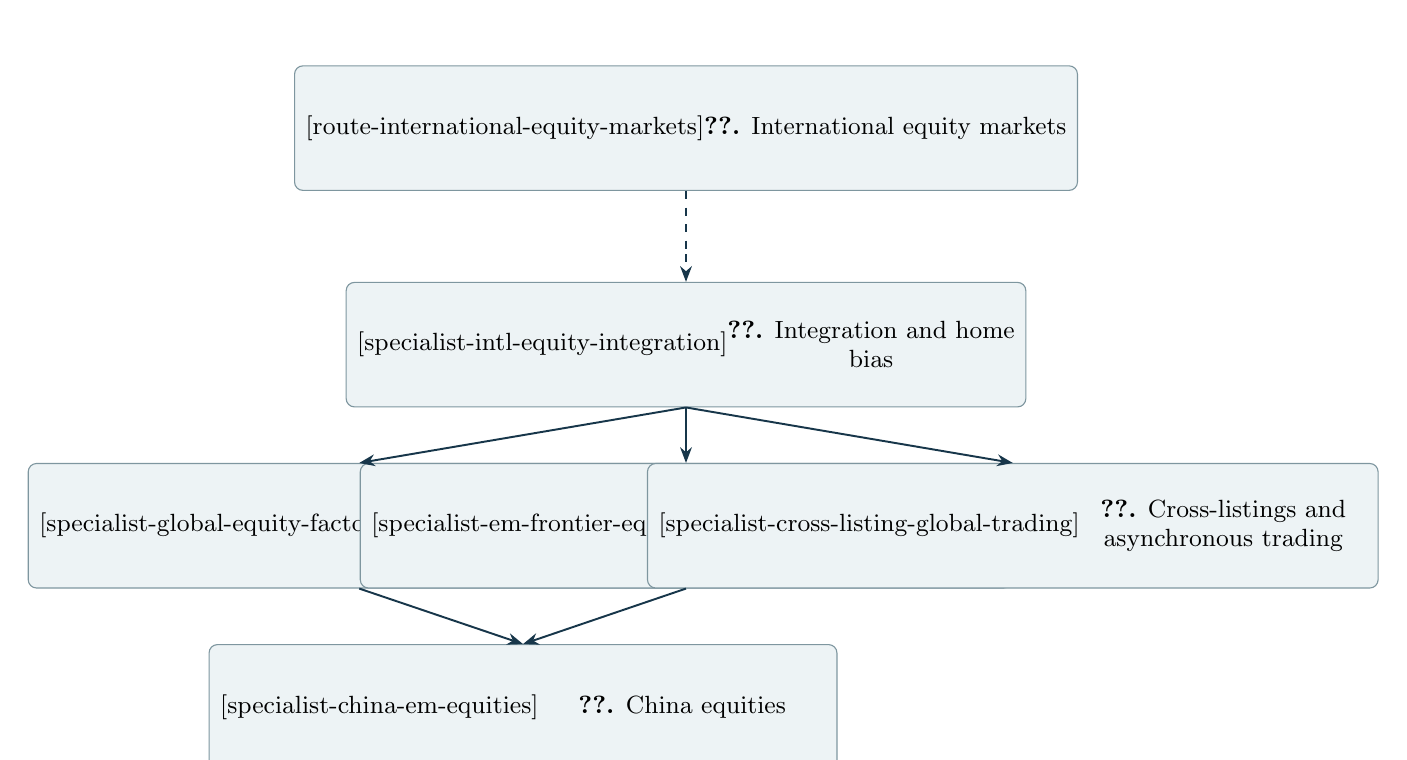
\begin{tikzpicture}[x=1cm,y=1cm]
\node[pathnode] (international-equity-markets) at (4.15,0) {\MeasurePathNode{4.6cm}{\textbf{\ref*{route-international-equity-markets}.} International equity markets}\hyperref[route-international-equity-markets]{\parbox[c][\pathnodeheight][c]{4.6cm}{\centering \textbf{\ref*{route-international-equity-markets}.} International equity markets}}};
\node[pathnode] (intl-equity-integration) at (4.15,-2.75) {\MeasurePathNode{3.65cm}{\textbf{\ref*{specialist-intl-equity-integration}.} Integration and home bias}\hyperref[specialist-intl-equity-integration]{\parbox[c][\pathnodeheight][c]{3.65cm}{\centering \textbf{\ref*{specialist-intl-equity-integration}.} Integration and home bias}}};
\node[pathnode] (global-equity-factors) at (0.00,-5.05) {\MeasurePathNode{3.65cm}{\textbf{\ref*{specialist-global-equity-factors}.} Global factors and country selection}\hyperref[specialist-global-equity-factors]{\parbox[c][\pathnodeheight][c]{3.65cm}{\centering \textbf{\ref*{specialist-global-equity-factors}.} Global factors and country selection}}};
\node[pathnode] (em-frontier-equities) at (4.15,-5.05) {\MeasurePathNode{3.65cm}{\textbf{\ref*{specialist-em-frontier-equities}.} Emerging and frontier equities}\hyperref[specialist-em-frontier-equities]{\parbox[c][\pathnodeheight][c]{3.65cm}{\centering \textbf{\ref*{specialist-em-frontier-equities}.} Emerging and frontier equities}}};
\node[pathnode] (cross-listing-global-trading) at (8.30,-5.05) {\MeasurePathNode{3.65cm}{\textbf{\ref*{specialist-cross-listing-global-trading}.} Cross-listings and asynchronous trading}\hyperref[specialist-cross-listing-global-trading]{\parbox[c][\pathnodeheight][c]{3.65cm}{\centering \textbf{\ref*{specialist-cross-listing-global-trading}.} Cross-listings and asynchronous trading}}};
\node[pathnode] (china-em-equities) at (2.08,-7.35) {\MeasurePathNode{3.65cm}{\textbf{\ref*{specialist-china-em-equities}.} China equities}\hyperref[specialist-china-em-equities]{\parbox[c][\pathnodeheight][c]{3.65cm}{\centering \textbf{\ref*{specialist-china-em-equities}.} China equities}}};
\draw[entryline] (international-equity-markets.south) -- (4.15,-1.60);
\draw[entryline] (4.15,-1.60) -- (4.15,-1.60);
\draw[entryarrow] (4.15,-1.60) -- (intl-equity-integration.north);
\draw[patharrow] (intl-equity-integration.south) -- (global-equity-factors.north);
\draw[patharrow] (intl-equity-integration.south) -- (em-frontier-equities.north);
\draw[patharrow] (intl-equity-integration.south) -- (cross-listing-global-trading.north);
\draw[patharrow] (global-equity-factors.south) -- (china-em-equities.north);
\draw[patharrow] (em-frontier-equities.south) -- (china-em-equities.north);
\end{tikzpicture}\end{center}
\textbf{Overview checkpoint.} A section capstone: complete it after \hyperref[specialist-intl-equity-integration]{\ref*{specialist-intl-equity-integration}}.

\textbf{Bring these foundations with you.}\begin{itemize}
\item \hyperref[specialist-equity-factor-premia]{Equity factor premia, crashes and timing} --- needed by \hyperref[specialist-global-equity-factors]{Global factors and country selection}, \hyperref[specialist-china-em-equities]{China equities}.
\end{itemize}\hyperref[learning-map]{Return to the whole-guide DAG.}
\Needspace{12\baselineskip}
\subsection{International equity integration, diversification and home bias}\label{specialist-intl-equity-integration}
\textbf{Specialist pathway.} In \hyperref[route-international-equity-markets]{International and emerging equity markets}.

\textbf{Outcome.} Price an asset under integration, mild segmentation and investment barriers; measure integration and diversification benefits with factor-based, copula and valuation measures rather than raw correlations; correct comovement tests for volatility; and explain home bias with hedging, cost, governance and information arguments.

\textbf{Prerequisites.} International and emerging equity markets overview; CAPM and factor models; currency risk premia for exchange-rate risk in international pricing.

\textbf{Review first.} \hyperref[route-international-equity-markets]{International and emerging equity markets}.

\textbf{Required readings, in order}
\begin{enumerate}\raggedright
\Needspace{5\baselineskip}\item \href{institutional_quantitative_finance_reading_list.pdf\#gr-solnik-1974}{Bruno H. Solnik, ``Why Not Diversify Internationally Rather Than Domestically?''}\CataloguePage{295}\NoteKey{gr-solnik-1974}\par \textbf{Foundations.} See the original case for international diversification from the low correlation of national markets.
\Needspace{5\baselineskip}\item \href{institutional_quantitative_finance_reading_list.pdf\#gr-adler-dumas-1983}{Michael Adler and Bernard Dumas, ``International Portfolio Choice and Corporation Finance: A Synthesis''}\CataloguePage{295}\NoteKey{gr-adler-dumas-1983}\par \textbf{Theory.} Learn international portfolio choice and asset pricing when purchasing-power parity fails.
\Needspace{5\baselineskip}\item \href{institutional_quantitative_finance_reading_list.pdf\#gr-stulz-1981}{Ren\'e M. Stulz, ``On the Effects of Barriers to International Investment''}\CataloguePage{295}\NoteKey{gr-stulz-1981}\par \textbf{Theory.} Model a proportional cost of holding foreign assets and the two security market lines it creates.
\Needspace{5\baselineskip}\item \href{institutional_quantitative_finance_reading_list.pdf\#gr-errunza-losq-1985}{Vihang Errunza and Etienne Losq, ``International Asset Pricing under Mild Segmentation: Theory and Test''}\CataloguePage{295}\NoteKey{gr-errunza-losq-1985}\par \textbf{Theory.} Price securities that some investors cannot hold: mild segmentation and super risk premia.
\Needspace{5\baselineskip}\item \href{institutional_quantitative_finance_reading_list.pdf\#w5-bekaert-harvey-integration}{Geert Bekaert and Campbell R. Harvey, ``Time-Varying World Market Integration''}\CataloguePage{294}\NoteKey{w5-bekaert-harvey-integration}\par \textbf{Evidence.} Estimate time-varying integration with a regime-switching model.
\Needspace{5\baselineskip}\item \href{institutional_quantitative_finance_reading_list.pdf\#gr-bekaert-harvey-lundblad-siegel-2011}{Geert Bekaert, Campbell R. Harvey, Christian T. Lundblad and Stephan Siegel, ``What Segments Equity Markets?''}\CataloguePage{297}\NoteKey{gr-bekaert-harvey-lundblad-siegel-2011}\par \textbf{Evidence.} Measure segmentation from valuations and relate it to capital controls, political risk and market development.
\Needspace{5\baselineskip}\item \href{institutional_quantitative_finance_reading_list.pdf\#gr-pukthuanthong-roll-2009}{Kuntara Pukthuanthong and Richard Roll, ``Global market integration: An alternative measure and its application''}\CataloguePage{297}\NoteKey{gr-pukthuanthong-roll-2009}\par \textbf{Data.} Measure integration by the explanatory power of global factors, not by correlations.
\Needspace{5\baselineskip}\item \href{institutional_quantitative_finance_reading_list.pdf\#gr-heston-rouwenhorst-1994}{Steven L. Heston and K. Geert Rouwenhorst, ``Does industrial structure explain the benefits of international diversification?''}\CataloguePage{296}\NoteKey{gr-heston-rouwenhorst-1994}\par \textbf{Evidence.} Decompose international returns into country and industry effects.
\Needspace{5\baselineskip}\item \href{institutional_quantitative_finance_reading_list.pdf\#gr-bekaert-hodrick-zhang-2009}{Geert Bekaert, Robert J. Hodrick and Xiaoyan Zhang, ``International Stock Return Comovements''}\CataloguePage{296}\NoteKey{gr-bekaert-hodrick-zhang-2009}\par \textbf{Evidence.} Test trends in comovement, and the short-lived rise of industry factors, with risk-based factor models.
\Needspace{5\baselineskip}\item \href{institutional_quantitative_finance_reading_list.pdf\#gr-forbes-rigobon-2002}{Kristin J. Forbes and Roberto Rigobon, ``No Contagion, Only Interdependence: Measuring Stock Market Comovements''}\CataloguePage{297}\NoteKey{gr-forbes-rigobon-2002}\par \textbf{Evidence.} Correct crisis correlations for heteroskedasticity before calling comovement contagion.
\Needspace{5\baselineskip}\item \href{institutional_quantitative_finance_reading_list.pdf\#gr-christoffersen-errunza-jacobs-langlois-2012}{Peter Christoffersen, Vihang Errunza, Kris Jacobs and Hugues Langlois, ``Is the Potential for International Diversification Disappearing? A Dynamic Copula Approach''}\CataloguePage{297}\NoteKey{gr-christoffersen-errunza-jacobs-langlois-2012}\par \textbf{Evidence.} Measure diversification benefits with dynamic asymmetric copulas and tail dependence.
\Needspace{5\baselineskip}\item \href{institutional_quantitative_finance_reading_list.pdf\#gr-anarkulova-cederburg-odoherty-2022}{Aizhan Anarkulova, Scott Cederburg and Michael S. O'Doherty, ``Stocks for the long run? Evidence from a broad sample of developed markets''}\CataloguePage{298}\NoteKey{gr-anarkulova-cederburg-odoherty-2022}\par \textbf{Evidence.} Bootstrap 30-year outcomes from 39 developed markets and the risk of losing to inflation.
\Needspace{5\baselineskip}\item \href{institutional_quantitative_finance_reading_list.pdf\#gr-french-poterba-1991}{Kenneth R. French and James M. Poterba, ``Investor Diversification and International Equity Markets''}\CataloguePage{295}\NoteKey{gr-french-poterba-1991}\par \textbf{Evidence.} Quantify home bias in US, Japanese and British portfolios and the return beliefs it implies.
\Needspace{5\baselineskip}\item \href{institutional_quantitative_finance_reading_list.pdf\#gr-ahearne-griever-warnock-2004}{Alan G. Ahearne, William L. Griever and Francis E. Warnock, ``Information costs and home bias: an analysis of U.S. holdings of foreign equities''}\CataloguePage{296}\NoteKey{gr-ahearne-griever-warnock-2004}\par \textbf{Evidence.} Relate US holdings to the share of a country's market listed in the US.
\Needspace{5\baselineskip}\item \href{institutional_quantitative_finance_reading_list.pdf\#gr-dahlquist-pinkowitz-stulz-williamson-2003}{Magnus Dahlquist, Lee Pinkowitz, Ren\'e M. Stulz and Rohan Williamson, ``Corporate Governance and the Home Bias''}\CataloguePage{296}\NoteKey{gr-dahlquist-pinkowitz-stulz-williamson-2003}\par \textbf{Evidence.} Benchmark holdings against the shares available to outside investors, not market capitalisation.
\Needspace{5\baselineskip}\item \href{institutional_quantitative_finance_reading_list.pdf\#gr-van-nieuwerburgh-veldkamp-2009}{Stijn Van Nieuwerburgh and Laura Veldkamp, ``Information Immobility and the Home Bias Puzzle''}\CataloguePage{296}\NoteKey{gr-van-nieuwerburgh-veldkamp-2009}\par \textbf{Theory.} See why investors with a small home information advantage choose to deepen it.
\end{enumerate}
\Needspace{5\baselineskip}\textbf{Checkpoint.} Using monthly MSCI country returns since 1990, estimate the Pukthuanthong--Roll integration measure and rolling correlations for 20 developed and emerging markets and show where they disagree. Re-run a crisis contagion test with and without the Forbes--Rigobon adjustment. Build a float-adjusted world portfolio, compare a US investor's country allocation (from TIC or IMF CPIS data) with it and with market-capitalisation weights, and report the home bias each benchmark implies.

\textbf{Optional branches.} \href{institutional_quantitative_finance_reading_list.pdf\#gr-kang-stulz-1997}{See which Japanese stocks foreign investors overweighted, and why.}\BranchPage{296} \href{institutional_quantitative_finance_reading_list.pdf\#gr-griffin-karolyi-1998}{Re-examine country and industry effects with 25 countries and 66 industries.}\BranchPage{296} \href{institutional_quantitative_finance_reading_list.pdf\#gr-goetzmann-li-rouwenhorst-2005}{Follow 150 years of global market correlations and diversification benefits.}\BranchPage{297} \href{institutional_quantitative_finance_reading_list.pdf\#gr-bae-karolyi-stulz-2003}{Measure contagion as coincident extreme returns.}\BranchPage{297} \href{institutional_quantitative_finance_reading_list.pdf\#gr-hardouvelis-malliaropulos-priestley-2006}{Trace European stock-market integration through the run-up to EMU.}\BranchPage{298} \href{institutional_quantitative_finance_reading_list.pdf\#w2-longin-solnik}{Study correlation in extreme markets with extreme-value methods.}\BranchPage{19} \href{institutional_quantitative_finance_reading_list.pdf\#ma-ang-bekaert-2002}{Allocate internationally when correlations switch regimes.}\BranchPage{269}
\par{\small \hyperref[learning-map]{Learning pathway DAG} \textbar{} \hyperref[route-international-equity-markets]{Section overview} \textbar{} \hyperref[map-international-equity-markets]{Section DAG}\NoteKey{intl-equity-integration}}
\Needspace{12\baselineskip}
\subsection{Global equity factors, country selection and return predictability}\label{specialist-global-equity-factors}
\textbf{Specialist pathway.} In \hyperref[route-international-equity-markets]{International and emerging equity markets}.

\textbf{Outcome.} Replicate value, momentum, profitability and investment premia across countries; choose between global, local and partially segmented factor models; build country-selection strategies from momentum, reversal and value; and test cross-country lead--lag and liquidity effects.

\textbf{Prerequisites.} International equity integration; equity factor premia, crashes and timing.

\textbf{Review first.} \hyperref[route-international-equity-markets]{International and emerging equity markets}; \hyperref[specialist-intl-equity-integration]{International equity integration, diversification and home bias}; \hyperref[specialist-equity-factor-premia]{Equity factor premia, crashes and timing}.

\textbf{Required readings, in order}
\begin{enumerate}\raggedright
\Needspace{5\baselineskip}\item \href{institutional_quantitative_finance_reading_list.pdf\#gr-fama-french-1998}{Eugene F. Fama and Kenneth R. French, ``Value versus Growth: The International Evidence''}\CataloguePage{298}\NoteKey{gr-fama-french-1998}\par \textbf{Evidence.} Find the value premium in twelve of thirteen markets and price it with a global distress factor.
\Needspace{5\baselineskip}\item \href{institutional_quantitative_finance_reading_list.pdf\#gr-rouwenhorst-1998}{K. Geert Rouwenhorst, ``International Momentum Strategies''}\CataloguePage{298}\NoteKey{gr-rouwenhorst-1998}\par \textbf{Evidence.} Replicate momentum in twelve European markets.
\Needspace{5\baselineskip}\item \href{institutional_quantitative_finance_reading_list.pdf\#gr-griffin-2002}{John M. Griffin, ``Are the Fama and French Factors Global or Country Specific?''}\CataloguePage{298}\NoteKey{gr-griffin-2002}\par \textbf{Evidence.} Compare country-specific and world three-factor models for pricing and the cost of capital.
\Needspace{5\baselineskip}\item \href{institutional_quantitative_finance_reading_list.pdf\#wide-hou-global-anomalies}{Kewei Hou, G. Andrew Karolyi and Bong-Chan Kho, ``What Factors Drive Global Stock Returns?''}\CataloguePage{298}\NoteKey{wide-hou-global-anomalies}\par \textbf{Evidence.} Compare factor evidence across 49 countries.
\Needspace{5\baselineskip}\item \href{institutional_quantitative_finance_reading_list.pdf\#w5-fama-french-intl-2012}{Eugene F. Fama and Kenneth R. French, ``Size, value, and momentum in international stock returns''}\CataloguePage{298}\NoteKey{w5-fama-french-intl-2012}\par \textbf{Evidence.} Compare size, value and momentum by region and test global against local models.
\Needspace{5\baselineskip}\item \href{institutional_quantitative_finance_reading_list.pdf\#gr-fama-french-2017}{Eugene F. Fama and Kenneth R. French, ``International tests of a five-factor asset pricing model''}\CataloguePage{299}\NoteKey{gr-fama-french-2017}\par \textbf{Evidence.} Test the five-factor model in North America, Europe, Japan and Asia Pacific.
\Needspace{5\baselineskip}\item \href{institutional_quantitative_finance_reading_list.pdf\#gr-karolyi-wu-2018}{G. Andrew Karolyi and Ying Wu, ``A New Partial-Segmentation Approach to Modeling International Stock Returns''}\CataloguePage{299}\NoteKey{gr-karolyi-wu-2018}\par \textbf{Valuation.} Build factors in a partial-segmentation framework that respects investability.
\Needspace{5\baselineskip}\item \href{institutional_quantitative_finance_reading_list.pdf\#gr-griffin-ji-martin-2003}{John M. Griffin, Xiuqing Ji and J. Spencer Martin, ``Momentum Investing and Business Cycle Risk: Evidence from Pole to Pole''}\CataloguePage{299}\NoteKey{gr-griffin-ji-martin-2003}\par \textbf{Evidence.} Check whether macroeconomic risk explains momentum around the world.
\Needspace{5\baselineskip}\item \href{institutional_quantitative_finance_reading_list.pdf\#gr-chui-titman-wei-2010}{Andy C. W. Chui, Sheridan Titman and K. C. John Wei, ``Individualism and Momentum around the World''}\CataloguePage{299}\NoteKey{gr-chui-titman-wei-2010}\par \textbf{Evidence.} Relate momentum profits to individualism and other country traits.
\Needspace{5\baselineskip}\item \href{institutional_quantitative_finance_reading_list.pdf\#w2-jacobs-muller}{Heiko Jacobs and Sebastian Müller, ``Anomalies across the globe: Once public, no longer existent?''}\CataloguePage{88}\NoteKey{w2-jacobs-muller}\par \textbf{Evidence.} See whether anomalies decay after publication outside the US.
\Needspace{5\baselineskip}\item \href{institutional_quantitative_finance_reading_list.pdf\#gr-richards-1997}{Anthony J. Richards, ``Winner-Loser Reversals in National Stock Market Indices: Can They be Explained?''}\CataloguePage{299}\NoteKey{gr-richards-1997}\par \textbf{Evidence.} Test winner--loser reversals in national indices.
\Needspace{5\baselineskip}\item \href{institutional_quantitative_finance_reading_list.pdf\#gr-balvers-wu-gilliland-2000}{Ronald Balvers, Yangru Wu and Erik Gilliland, ``Mean Reversion across National Stock Markets and Parametric Contrarian Investment Strategies''}\CataloguePage{299}\NoteKey{gr-balvers-wu-gilliland-2000}\par \textbf{Implementation.} Exploit mean reversion in relative national index prices with a parametric contrarian rule.
\Needspace{5\baselineskip}\item \href{institutional_quantitative_finance_reading_list.pdf\#ma-asness-liew-stevens-1997}{Clifford S. Asness, John M. Liew and Ross L. Stevens, ``Parallels Between the Cross-Sectional Predictability of Stock and Country Returns''}\CataloguePage{265}\NoteKey{ma-asness-liew-stevens-1997}\par \textbf{Evidence.} Apply stock-level value and momentum signals to country selection.
\Needspace{5\baselineskip}\item \href{institutional_quantitative_finance_reading_list.pdf\#gr-rapach-strauss-zhou-2013}{David E. Rapach, Jack K. Strauss and Guofu Zhou, ``International Stock Return Predictability: What Is the Role of the United States?''}\CataloguePage{299}\NoteKey{gr-rapach-strauss-zhou-2013}\par \textbf{Evidence.} Test whether lagged US returns predict other markets.
\Needspace{5\baselineskip}\item \href{institutional_quantitative_finance_reading_list.pdf\#gr-amihud-hameed-kang-zhang-2015}{Yakov Amihud, Allaudeen Hameed, Wenjin Kang and Huiping Zhang, ``The illiquidity premium: International evidence''}\CataloguePage{299}\NoteKey{gr-amihud-hameed-kang-zhang-2015}\par \textbf{Evidence.} Measure the illiquidity premium across 45 countries.
\Needspace{5\baselineskip}\item \href{institutional_quantitative_finance_reading_list.pdf\#gr-karolyi-lee-van-dijk-2012}{G. Andrew Karolyi, Kuan-Hui Lee and Mathijs A. van Dijk, ``Understanding commonality in liquidity around the world''}\CataloguePage{300}\NoteKey{gr-karolyi-lee-van-dijk-2012}\par \textbf{Evidence.} Relate commonality in liquidity and returns to investor protection, opacity and openness.
\end{enumerate}
\Needspace{5\baselineskip}\textbf{Checkpoint.} From a point-in-time global stock file (Compustat Global or the JKP data), construct value, momentum, profitability and investment factors for 20 markets with local, regional and global breakpoints. Compare pricing errors of local, global and partially segmented models on country size and book-to-market portfolios, and test factor returns before and after their US publication dates. Separately build a country-selection portfolio from index momentum, three- to five-year reversal and valuation, rebalanced monthly in US dollars, and report it after transaction costs against an all-country benchmark.

\textbf{Optional branches.} \href{institutional_quantitative_finance_reading_list.pdf\#gr-lee-2011}{Test the liquidity-adjusted CAPM on a global scale.}\BranchPage{300} \href{institutional_quantitative_finance_reading_list.pdf\#gr-ang-hodrick-xing-zhang-2009}{Check the idiosyncratic-volatility puzzle in 23 developed markets.}\BranchPage{300} \href{institutional_quantitative_finance_reading_list.pdf\#gr-chan-hamao-lakonishok-1991}{Read early out-of-US evidence on value from Japan.}\BranchPage{300} \href{institutional_quantitative_finance_reading_list.pdf\#w5-baltussen-global-premiums}{Test factor premia over two centuries and across asset classes.}\BranchPage{194} \href{institutional_quantitative_finance_reading_list.pdf\#exp-jkp-replication}{Use the global factor dataset for replication across countries.}\BranchPage{87}
\par{\small \hyperref[learning-map]{Learning pathway DAG} \textbar{} \hyperref[route-international-equity-markets]{Section overview} \textbar{} \hyperref[map-international-equity-markets]{Section DAG}\NoteKey{global-equity-factors}}
\Needspace{12\baselineskip}
\subsection{Emerging and frontier equity markets: liberalisation, foreign investors and liquidity}\label{specialist-em-frontier-equities}
\textbf{Specialist pathway.} In \hyperref[route-international-equity-markets]{International and emerging equity markets}.

\textbf{Outcome.} Explain how liberalisation changes prices, the cost of capital and growth; measure liquidity and price informativeness where trading is thin; assess the impact of foreign investors' trading; adapt factor research to emerging and frontier markets; and apply index-provider classification criteria.

\textbf{Prerequisites.} International equity integration.

\textbf{Review first.} \hyperref[route-international-equity-markets]{International and emerging equity markets}; \hyperref[specialist-intl-equity-integration]{International equity integration, diversification and home bias}.

\textbf{Required readings, in order}
\begin{enumerate}\raggedright
\Needspace{5\baselineskip}\item \href{institutional_quantitative_finance_reading_list.pdf\#gr-harvey-1995}{Campbell R. Harvey, ``Predictable Risk and Returns in Emerging Markets''}\CataloguePage{303}\NoteKey{gr-harvey-1995}\par \textbf{Evidence.} See why global pricing models fail in emerging markets and why local information predicts returns.
\Needspace{5\baselineskip}\item \href{institutional_quantitative_finance_reading_list.pdf\#gr-henry-2000}{Peter Blair Henry, ``Stock Market Liberalization, Economic Reform, and Emerging Market Equity Prices''}\CataloguePage{303}\NoteKey{gr-henry-2000}\par \textbf{Evidence.} Measure abnormal returns as markets open to foreign investors.
\Needspace{5\baselineskip}\item \href{institutional_quantitative_finance_reading_list.pdf\#gr-kim-singal-2000}{E. Han Kim and Vijay Singal, ``Stock Market Openings: Experience of Emerging Economies''}\CataloguePage{303}\NoteKey{gr-kim-singal-2000}\par \textbf{Evidence.} Check returns, volatility, inflation and exchange rates around market openings.
\Needspace{5\baselineskip}\item \href{institutional_quantitative_finance_reading_list.pdf\#w5-bekaert-harvey-speculators}{Geert Bekaert and Campbell R. Harvey, ``Foreign Speculators and Emerging Equity Markets''}\CataloguePage{303}\NoteKey{w5-bekaert-harvey-speculators}\par \textbf{Evidence.} Estimate how liberalisation changes the cost of capital and correlation with world markets.
\Needspace{5\baselineskip}\item \href{institutional_quantitative_finance_reading_list.pdf\#gr-bekaert-harvey-lundblad-2005}{Geert Bekaert, Campbell R. Harvey and Christian Lundblad, ``Does financial liberalization spur growth?''}\CataloguePage{304}\NoteKey{gr-bekaert-harvey-lundblad-2005}\par \textbf{Evidence.} Relate equity liberalisation to faster economic growth.
\Needspace{5\baselineskip}\item \href{institutional_quantitative_finance_reading_list.pdf\#gr-bekaert-harvey-lundblad-siegel-2007}{Geert Bekaert, Campbell R. Harvey, Christian Lundblad and Stephan Siegel, ``Global Growth Opportunities and Market Integration''}\CataloguePage{304}\NoteKey{gr-bekaert-harvey-lundblad-siegel-2007}\par \textbf{Evidence.} Measure growth opportunities from global PE ratios and test whether openness aligns them with growth.
\Needspace{5\baselineskip}\item \href{institutional_quantitative_finance_reading_list.pdf\#w5-bekaert-harvey-lundblad-liquidity}{Geert Bekaert, Campbell R. Harvey and Christian Lundblad, ``Liquidity and Expected Returns: Lessons from Emerging Markets''}\CataloguePage{303}\NoteKey{w5-bekaert-harvey-lundblad-liquidity}\par \textbf{Evidence.} Price liquidity in emerging markets with zero-return measures.
\Needspace{5\baselineskip}\item \href{institutional_quantitative_finance_reading_list.pdf\#gr-morck-yeung-yu-2000}{Randall Morck, Bernard Yeung and Wayne Yu, ``The information content of stock markets: why do emerging markets have synchronous stock price movements?''}\CataloguePage{304}\NoteKey{gr-morck-yeung-yu-2000}\par \textbf{Evidence.} Relate stock-price synchronicity to property rights.
\Needspace{5\baselineskip}\item \href{institutional_quantitative_finance_reading_list.pdf\#w5-griffin-kelly-nardari}{John M. Griffin, Patrick J. Kelly and Federico Nardari, ``Do Market Efficiency Measures Yield Correct Inferences? A Comparison of Developed and Emerging Markets''}\CataloguePage{303}\NoteKey{w5-griffin-kelly-nardari}\par \textbf{Data.} See why standard efficiency measures can misrank developed and emerging markets.
\Needspace{5\baselineskip}\item \href{institutional_quantitative_finance_reading_list.pdf\#gr-choe-kho-stulz-1999}{Hyuk Choe, Bong-Chan Kho and Ren\'e M. Stulz, ``Do foreign investors destabilize stock markets? The Korean experience in 1997''}\CataloguePage{304}\NoteKey{gr-choe-kho-stulz-1999}\par \textbf{Evidence.} Test whether foreign investors destabilised Korea's market in 1997.
\Needspace{5\baselineskip}\item \href{institutional_quantitative_finance_reading_list.pdf\#gr-richards-2005}{Anthony Richards, ``Big Fish in Small Ponds: The Trading Behavior and Price Impact of Foreign Investors in Asian Emerging Equity Markets''}\CataloguePage{304}\NoteKey{gr-richards-2005}\par \textbf{Evidence.} Measure foreign investors' feedback trading and price impact in six Asian markets.
\Needspace{5\baselineskip}\item \href{institutional_quantitative_finance_reading_list.pdf\#w5-rouwenhorst-em-factors}{K. Geert Rouwenhorst, ``Local Return Factors and Turnover in Emerging Stock Markets''}\CataloguePage{303}\NoteKey{w5-rouwenhorst-em-factors}\par \textbf{Evidence.} Test size, value and momentum in 20 emerging markets.
\Needspace{5\baselineskip}\item \href{institutional_quantitative_finance_reading_list.pdf\#gr-de-groot-pang-swinkels-2012}{Wilma de Groot, Juan Pang and Laurens Swinkels, ``The cross-section of stock returns in frontier emerging markets''}\CataloguePage{304}\NoteKey{gr-de-groot-pang-swinkels-2012}\par \textbf{Evidence.} Find value, momentum and local size effects in 24 frontier markets after costs.
\Needspace{5\baselineskip}\item \href{institutional_quantitative_finance_reading_list.pdf\#gr-berger-pukthuanthong-yang-2011}{Dave Berger, Kuntara Pukthuanthong and J. Jimmy Yang, ``International diversification with frontier markets''}\CataloguePage{304}\NoteKey{gr-berger-pukthuanthong-yang-2011}\par \textbf{Evidence.} Measure frontier markets' low integration and diversification value.
\Needspace{5\baselineskip}\item \href{institutional_quantitative_finance_reading_list.pdf\#gr-ftse-country-classification-2026}{FTSE Russell (LSEG), FTSE Russell announces results of September 2026 annual country classification review for equities and fixed income}\CataloguePage{315}\NoteKey{gr-ftse-country-classification-2026}\par \textbf{Regulation.} Follow an index provider's reclassifications: Greece, Vietnam and Nigeria in September 2026.
\Needspace{5\baselineskip}\item \href{institutional_quantitative_finance_reading_list.pdf\#gap-india-markets}{Sanjay Malhotra, Reserve Bank of India, Indian financial markets: resilience and resurgence}\CataloguePage{310}\NoteKey{gap-india-markets}\par \textbf{Evidence.} Read a central-bank account of Indian market development as a current case.
\end{enumerate}
\Needspace{5\baselineskip}\textbf{Checkpoint.} For five markets that liberalised between 1986 and 1995, estimate event-time abnormal dollar returns and changes in dividend yields around the official liberalisation date. For a current emerging and a frontier market, compute zero-return, Amihud and synchronicity measures from daily data and compare them with a developed market. Replicate value and momentum with local breakpoints net of costs based on quoted spreads, and document which FTSE or MSCI accessibility criteria the frontier market fails.

\textbf{Optional branches.} \href{institutional_quantitative_finance_reading_list.pdf\#gr-cakici-fabozzi-tan-2013}{Compare local, US and global factor models in 18 emerging markets.}\BranchPage{304} \href{institutional_quantitative_finance_reading_list.pdf\#gr-hanauer-lauterbach-2019}{Test which factor definitions are robust in 28 emerging markets.}\BranchPage{305} \href{institutional_quantitative_finance_reading_list.pdf\#gr-bhattacharya-daouk-2002}{See the cost of equity fall after the first insider-trading prosecution.}\BranchPage{305} \href{institutional_quantitative_finance_reading_list.pdf\#gr-la-porta-et-al-1998}{Relate investor protection and ownership concentration to legal origin.}\BranchPage{305}
\par{\small \hyperref[learning-map]{Learning pathway DAG} \textbar{} \hyperref[route-international-equity-markets]{Section overview} \textbar{} \hyperref[map-international-equity-markets]{Section DAG}\NoteKey{em-frontier-equities}}
\Needspace{12\baselineskip}
\subsection{Cross-listings, ADRs and asynchronous global trading}\label{specialist-cross-listing-global-trading}
\textbf{Specialist pathway.} In \hyperref[route-international-equity-markets]{International and emerging equity markets}.

\textbf{Outcome.} Explain why firms cross-list and what listing does to value, liquidity and price discovery; measure ADR and dual-listed parity deviations and the limits to arbitrage; model transmission across non-overlapping trading hours; and correct correlations, fund NAVs and country-ETF prices for stale prices.

\textbf{Prerequisites.} International equity integration; market microstructure and price discovery (Part III).

\textbf{Review first.} \hyperref[route-international-equity-markets]{International and emerging equity markets}; \hyperref[specialist-intl-equity-integration]{International equity integration, diversification and home bias}.

\textbf{Required readings, in order}
\begin{enumerate}\raggedright
\Needspace{5\baselineskip}\item \href{institutional_quantitative_finance_reading_list.pdf\#gr-karolyi-2006}{G. Andrew Karolyi, ``The World of Cross-Listings and Cross-Listings of the World: Challenging Conventional Wisdom''}\CataloguePage{300}\NoteKey{gr-karolyi-2006}\par \textbf{Foundations.} Survey why firms list abroad and the governance and information evidence that challenged the cost-of-capital view.
\Needspace{5\baselineskip}\item \href{institutional_quantitative_finance_reading_list.pdf\#gr-foerster-karolyi-1999}{Stephen R. Foerster and G. Andrew Karolyi, ``The Effects of Market Segmentation and Investor Recognition on Asset Prices: Evidence from Foreign Stocks Listing in the United States''}\CataloguePage{300}\NoteKey{gr-foerster-karolyi-1999}\par \textbf{Evidence.} Measure returns around US listings and relate them to investor recognition.
\Needspace{5\baselineskip}\item \href{institutional_quantitative_finance_reading_list.pdf\#gr-doidge-karolyi-stulz-2004}{Craig Doidge, G. Andrew Karolyi and Ren\'e M. Stulz, ``Why are foreign firms listed in the U.S. worth more?''}\CataloguePage{300}\NoteKey{gr-doidge-karolyi-stulz-2004}\par \textbf{Evidence.} Explain the valuation premium of US-listed foreign firms with bonding and growth opportunities.
\Needspace{5\baselineskip}\item \href{institutional_quantitative_finance_reading_list.pdf\#gr-halling-pagano-randl-zechner-2008}{Michael Halling, Marco Pagano, Otto Randl and Josef Zechner, ``Where Is the Market? Evidence from Cross-Listings in the United States''}\CataloguePage{301}\NoteKey{gr-halling-pagano-randl-zechner-2008}\par \textbf{Evidence.} Find where cross-listed stocks actually trade, and why.
\Needspace{5\baselineskip}\item \href{institutional_quantitative_finance_reading_list.pdf\#gr-eun-sabherwal-2003}{Cheol S. Eun and Sanjiv Sabherwal, ``Cross-Border Listings and Price Discovery: Evidence from U.S.-Listed Canadian Stocks''}\CataloguePage{301}\NoteKey{gr-eun-sabherwal-2003}\par \textbf{Evidence.} Measure the US share of price discovery for Canadian cross-listings.
\Needspace{5\baselineskip}\item \href{institutional_quantitative_finance_reading_list.pdf\#gr-gagnon-karolyi-2010}{Louis Gagnon and G. Andrew Karolyi, ``Multi-market trading and arbitrage''}\CataloguePage{301}\NoteKey{gr-gagnon-karolyi-2010}\par \textbf{Evidence.} Measure intraday ADR parity deviations and relate them to holding costs.
\Needspace{5\baselineskip}\item \href{institutional_quantitative_finance_reading_list.pdf\#gr-rosenthal-young-1990}{Leonard Rosenthal and Colin Young, ``The seemingly anomalous price behavior of Royal Dutch/Shell and Unilever N.V./PLC''}\CataloguePage{301}\NoteKey{gr-rosenthal-young-1990}\par \textbf{Evidence.} See the Royal Dutch/Shell and Unilever twin-share deviations.
\Needspace{5\baselineskip}\item \href{institutional_quantitative_finance_reading_list.pdf\#gr-froot-dabora-1999}{Kenneth A. Froot and Emil M. Dabora, ``How are stock prices affected by the location of trade?''}\CataloguePage{301}\NoteKey{gr-froot-dabora-1999}\par \textbf{Evidence.} Relate twin-share prices to the markets where each line trades.
\Needspace{5\baselineskip}\item \href{institutional_quantitative_finance_reading_list.pdf\#gr-de-jong-rosenthal-van-dijk-2009}{Abe de Jong, Leonard Rosenthal and Mathijs A. van Dijk, ``The Risk and Return of Arbitrage in Dual-Listed Companies''}\CataloguePage{301}\NoteKey{gr-de-jong-rosenthal-van-dijk-2009}\par \textbf{Implementation.} Evaluate dual-listed arbitrage returns and the horizon risk that limits them.
\Needspace{5\baselineskip}\item \href{institutional_quantitative_finance_reading_list.pdf\#gr-pasquariello-2014}{Paolo Pasquariello, ``Financial Market Dislocations''}\CataloguePage{302}\NoteKey{gr-pasquariello-2014}\par \textbf{Evidence.} Aggregate ADR, triangular and covered-interest-parity violations into a dislocation measure and price it.
\Needspace{5\baselineskip}\item \href{institutional_quantitative_finance_reading_list.pdf\#gr-hamao-masulis-ng-1990}{Yasushi Hamao, Ronald W. Masulis and Victor Ng, ``Correlations in Price Changes and Volatility across International Stock Markets''}\CataloguePage{302}\NoteKey{gr-hamao-masulis-ng-1990}\par \textbf{Evidence.} Trace volatility spillovers between Tokyo, London and New York.
\Needspace{5\baselineskip}\item \href{institutional_quantitative_finance_reading_list.pdf\#gr-lin-engle-ito-1994}{Wen-Ling Lin, Robert F. Engle and Takatoshi Ito, ``Do Bulls and Bears Move Across Borders? International Transmission of Stock Returns and Volatility''}\CataloguePage{302}\NoteKey{gr-lin-engle-ito-1994}\par \textbf{Evidence.} Separate daytime and overnight returns to see information cross from New York to Tokyo.
\Needspace{5\baselineskip}\item \href{institutional_quantitative_finance_reading_list.pdf\#gr-burns-engle-mezrich-1998}{Patrick Burns, Robert F. Engle and Joseph J. Mezrich, ``Correlations and Volatilities of Asynchronous Data''}\CataloguePage{302}\NoteKey{gr-burns-engle-mezrich-1998}\par \textbf{Valuation.} Synchronise returns across closing times before estimating correlations and VaR.
\Needspace{5\baselineskip}\item \href{institutional_quantitative_finance_reading_list.pdf\#gr-goetzmann-ivkovic-rouwenhorst-2001}{William N. Goetzmann, Zoran Ivkovi\'c and K. Geert Rouwenhorst, ``Day Trading International Mutual Funds: Evidence and Policy Solutions''}\CataloguePage{302}\NoteKey{gr-goetzmann-ivkovic-rouwenhorst-2001}\par \textbf{Implementation.} See how stale NAVs let traders exploit international funds, and how fair-value pricing stops it.
\Needspace{5\baselineskip}\item \href{institutional_quantitative_finance_reading_list.pdf\#gr-levy-lieberman-2013}{Ariel Levy and Offer Lieberman, ``Overreaction of country ETFs to US market returns: Intraday vs. daily horizons and the role of synchronized trading''}\CataloguePage{302}\NoteKey{gr-levy-lieberman-2013}\par \textbf{Evidence.} Study country-ETF pricing while the underlying market is closed.
\end{enumerate}
\Needspace{5\baselineskip}\textbf{Checkpoint.} For ten ADRs from three time zones, align home-market and US quotes at synchronous minutes, convert at the matching spot rate and compute parity deviations net of the depositary ratio and fees. Relate the deviations to borrowing costs and FX volatility, and estimate information shares during overlapping hours. Then synchronise daily G7 index returns with the Burns--Engle--Mezrich method, compare synchronised and close-to-close correlations, and back-test a stale-NAV trading rule on an international fund with and without fair-value pricing.

\textbf{Optional branches.} \href{institutional_quantitative_finance_reading_list.pdf\#gr-grammig-melvin-schlag-2005}{Measure home and US price discovery during overlapping hours.}\BranchPage{301} \href{institutional_quantitative_finance_reading_list.pdf\#gr-petajisto-2017}{Measure ETF premiums and discounts after correcting for stale NAVs.}\BranchPage{302}
\par{\small \hyperref[learning-map]{Learning pathway DAG} \textbar{} \hyperref[route-international-equity-markets]{Section overview} \textbar{} \hyperref[map-international-equity-markets]{Section DAG}\NoteKey{cross-listing-global-trading}}
\Needspace{12\baselineskip}
\subsection{China's stock market: factors, retail trading, intervention and access}\label{specialist-china-em-equities}
\textbf{Specialist pathway.} In \hyperref[route-international-equity-markets]{International and emerging equity markets}.

\textbf{Outcome.} Adapt factor and machine-learning equity research to China, accounting for reverse-merger shell value, retail flow, price limits, margin leverage and state intervention, and for access through Stock Connect.

\textbf{Prerequisites.} Global equity factors; emerging and frontier equity markets; equity factor premia, crashes and timing.

\textbf{Review first.} \hyperref[route-international-equity-markets]{International and emerging equity markets}; \hyperref[specialist-global-equity-factors]{Global equity factors, country selection and return predictability}; \hyperref[specialist-em-frontier-equities]{Emerging and frontier equity markets: liberalisation, foreign investors and liquidity}; \hyperref[specialist-equity-factor-premia]{Equity factor premia, crashes and timing}.

\textbf{Required readings, in order}
\begin{enumerate}\raggedright
\Needspace{5\baselineskip}\item \href{institutional_quantitative_finance_reading_list.pdf\#w5-hu-pan-wang-china}{Grace Xing Hu, Jun Pan and Jiang Wang, ``Chinese Capital Market: An Empirical Overview''}\CataloguePage{316}\NoteKey{w5-hu-pan-wang-china}\par \textbf{Foundations.} Start with a data-rich overview of China's equity and bond markets.
\Needspace{5\baselineskip}\item \href{institutional_quantitative_finance_reading_list.pdf\#gr-song-xiong-2018}{Zheng (Michael) Song and Wei Xiong, ``Risks in China's Financial System''}\CataloguePage{316}\NoteKey{gr-song-xiong-2018}\par \textbf{Foundations.} Place market risks in China's state-led financial system.
\Needspace{5\baselineskip}\item \href{institutional_quantitative_finance_reading_list.pdf\#w2-allen-china-performance}{Franklin Allen, Jun (QJ) Qian, Chenyu Shan and Julie Lei Zhu, ``Dissecting the Long-Term Performance of the Chinese Stock Market''}\CataloguePage{315}\NoteKey{w2-allen-china-performance}\par \textbf{Evidence.} Dissect the long-run underperformance of A-shares.
\Needspace{5\baselineskip}\item \href{institutional_quantitative_finance_reading_list.pdf\#wide-carpenter-china-value}{Jennifer N. Carpenter, Fangzhou Lu and Robert F. Whitelaw, ``The real value of China's stock market''}\CataloguePage{315}\NoteKey{wide-carpenter-china-value}\par \textbf{Evidence.} Assess informativeness of Chinese prices.
\Needspace{5\baselineskip}\item \href{institutional_quantitative_finance_reading_list.pdf\#wide-lsy-china}{Jianan Liu, Robert F. Stambaugh and Yu Yuan, ``Size and value in China''}\CataloguePage{315}\NoteKey{wide-lsy-china}\par \textbf{Evidence.} Use China-specific size and value factors that remove shell-value stocks.
\Needspace{5\baselineskip}\item \href{institutional_quantitative_finance_reading_list.pdf\#wide-leippold-wang-zhou-china}{Markus Leippold, Qian Wang and Wenyu Zhou, ``Machine learning in the Chinese stock market''}\CataloguePage{54}\NoteKey{wide-leippold-wang-zhou-china}\par \textbf{Evidence.} Replicate ML prediction in China.
\Needspace{5\baselineskip}\item \href{institutional_quantitative_finance_reading_list.pdf\#gr-jones-shi-zhang-zhang-2024}{Charles M. Jones, Donghui Shi, Xiaoyan Zhang and Xinran Zhang, ``Retail Trading and Return Predictability in China''}\CataloguePage{317}\NoteKey{gr-jones-shi-zhang-zhang-2024}\par \textbf{Evidence.} Separate retail investors by account size and see who predicts returns.
\Needspace{5\baselineskip}\item \href{institutional_quantitative_finance_reading_list.pdf\#gr-titman-wei-zhao-2022}{Sheridan Titman, Chishen Wei and Bin Zhao, ``Corporate actions and the manipulation of retail investors in China: An analysis of stock splits''}\CataloguePage{316}\NoteKey{gr-titman-wei-zhao-2022}\par \textbf{Evidence.} See how suspicious stock splits transfer wealth from small retail investors.
\Needspace{5\baselineskip}\item \href{institutional_quantitative_finance_reading_list.pdf\#gr-chen-gao-he-jiang-xiong-2019}{Ting Chen, Zhenyu Gao, Jibao He, Wenxi Jiang and Wei Xiong, ``Daily price limits and destructive market behavior''}\CataloguePage{316}\NoteKey{gr-chen-gao-he-jiang-xiong-2019}\par \textbf{Mechanics.} Study how daily price limits invite buying at the limit and later reversals.
\Needspace{5\baselineskip}\item \href{institutional_quantitative_finance_reading_list.pdf\#gr-bian-he-shue-zhou-2018}{Jiangze Bian, Zhiguo He, Kelly Shue and Hao Zhou, ``Leverage-Induced Fire Sales and Stock Market Crashes''}\CataloguePage{316}\NoteKey{gr-bian-he-shue-zhou-2018}\par \textbf{Evidence.} Trace leverage-induced fire sales in the 2015 crash with account-level data.
\Needspace{5\baselineskip}\item \href{institutional_quantitative_finance_reading_list.pdf\#gr-huang-miao-wang-2019}{Yi Huang, Jianjun Miao and Pengfei Wang, ``Saving China's Stock Market?''}\CataloguePage{316}\NoteKey{gr-huang-miao-wang-2019}\par \textbf{Evidence.} Value the 2015 government share purchases.
\Needspace{5\baselineskip}\item \href{institutional_quantitative_finance_reading_list.pdf\#gr-chan-menkveld-yang-2008}{Kalok Chan, Albert J. Menkveld and Zhishu Yang, ``Information Asymmetry and Asset Prices: Evidence from the China Foreign Share Discount''}\CataloguePage{316}\NoteKey{gr-chan-menkveld-yang-2008}\par \textbf{Evidence.} Explain the B-share discount by information asymmetry.
\Needspace{5\baselineskip}\item \href{institutional_quantitative_finance_reading_list.pdf\#gap-stock-connect}{Hong Kong Exchanges and Clearing, Stock Connect: Information Books for Investors and Market Participants; Market participant book (6 July 2026)}\CataloguePage{310}\NoteKey{gap-stock-connect}\par \textbf{Mechanics.} Learn Stock Connect access mechanics.
\Needspace{5\baselineskip}\item \href{institutional_quantitative_finance_reading_list.pdf\#gr-ma-rogers-zhou-2019}{Chang Ma, John Rogers and Sili Zhou, ``The Effect of the China Connect''}\CataloguePage{317}\NoteKey{gr-ma-rogers-zhou-2019}\par \textbf{Evidence.} Estimate how Stock Connect changed connected firms' exposure to US monetary policy and their financing costs.
\Needspace{5\baselineskip}\item \href{institutional_quantitative_finance_reading_list.pdf\#depth-china-rmb-fx-evidence}{Juliana Robbert, Vladyslav Sushko and Frank Westermann, Shifting Forces behind RMB Internationalization: Evidence from the 2025 Triennial Survey}\CataloguePage{311}\NoteKey{depth-china-rmb-fx-evidence}\par \textbf{Evidence.} Relate RMB internationalisation to market access.
\end{enumerate}
\Needspace{5\baselineskip}\textbf{Checkpoint.} Replicate the Liu--Stambaugh--Yuan four-factor model after excluding the smallest 30 per cent of stocks, compare it with an unadjusted US-style model, and test a momentum or ML signal net of Stock Connect eligibility and limit-move rules. Flag special-treatment stocks with 5 per cent limits, mark the 2015 crash and state-purchase window, and report results with and without days on which a stock closed at its limit.

\textbf{Optional branches.} \href{institutional_quantitative_finance_reading_list.pdf\#crypto-whitepaper}{Read the China quantitative investment industry whitepaper for context.}\BranchPage{493} \href{institutional_quantitative_finance_reading_list.pdf\#gr-lee-qu-shen-2019}{Compare reverse mergers and IPOs to understand shell value.}\BranchPage{317} \href{institutional_quantitative_finance_reading_list.pdf\#gr-amstad-sun-xiong-2020}{Use the handbook chapters on banking, monetary policy, bonds, the stock market and capital-account liberalisation.}\BranchPage{317}
\par{\small \hyperref[learning-map]{Learning pathway DAG} \textbar{} \hyperref[route-international-equity-markets]{Section overview} \textbar{} \hyperref[map-international-equity-markets]{Section DAG}\NoteKey{china-em-equities}}
\clearpage
\section{Global and regional markets: capital flows, local bonds and market access}\label{route-global-regional-markets}
\label{route-15}
\textbf{Learning sequence.} Start with capital flows and benchmark-driven investors, then local-currency government bonds, then trace a security through access, custody, settlement, tax and hedging. Equity integration, emerging-market equities and China are in the previous section.

\textbf{Section goals.} Across its pathways, this section teaches you to:
\begin{itemize}[leftmargin=1.4em,itemsep=0pt,topsep=1pt]
\item separate push and pull drivers of capital flows and estimate benchmark-driven flow effects (\hyperref[specialist-em-capital-flows]{\ref*{specialist-em-capital-flows}})
\item decompose local-currency government bond yields and assess the risk from foreign holders (\hyperref[specialist-em-local-currency-bonds]{\ref*{specialist-em-local-currency-bonds}})
\item trace a local security through access, custody, settlement, tax, hedging and repatriation (\hyperref[specialist-regional-local-market-access]{\ref*{specialist-regional-local-market-access}})
\end{itemize}
\textbf{Overview outcome.} Compare the hedged returns of two local-currency government bond markets from dated records of eligibility, tax, trading calendar, price source, custody, settlement, FX hedge terms and rule versions, marking every input that is unavailable.

\textbf{Prerequisites.} The Currency markets and Government bond markets overviews; settlement and macro data releases. The first pathway brings Emerging-market currencies, intervention and the global financial cycle (13.7), and the second Sovereign default, restructuring and local-currency debt (6.3). International equity markets precede this section.

\textbf{Review first.} \hyperref[route-government-bond-markets]{Government bond markets and sovereign debt}; \hyperref[route-currency-markets]{Currency markets: exchange rates, premia and hedging}.

\textbf{Required readings, in order}
\begin{enumerate}\raggedright
\Needspace{5\baselineskip}\item \href{institutional_quantitative_finance_reading_list.pdf\#gap-global-macro-database}{Karsten Müller, Chenzi Xu, Mohamed Lehbib and Ziliang Chen, The Global Macro Database: A New International Macroeconomic Dataset; Dataset paper}\CataloguePage{518}\NoteKey{gap-global-macro-database}\par Start with a documented cross-country macro panel and its comparability limits.
\Needspace{5\baselineskip}\item \href{institutional_quantitative_finance_reading_list.pdf\#gr-koepke-2019}{Robin Koepke, ``What Drives Capital Flows to Emerging Markets? A Survey of the Empirical Literature''}\CataloguePage{305}\NoteKey{gr-koepke-2019}\par Frame capital flows by push and pull drivers and by type of flow.
\Needspace{5\baselineskip}\item \href{institutional_quantitative_finance_reading_list.pdf\#gap-sovereign-local-currency}{Wenxin Du and Jesse Schreger, Local Currency Sovereign Risk}\CataloguePage{229}\NoteKey{gap-sovereign-local-currency}\par Separate local-currency sovereign credit risk from exchange-rate exposure.
\Needspace{5\baselineskip}\item \href{institutional_quantitative_finance_reading_list.pdf\#gap-cip}{Wenxin Du, Alexander Tepper and Adrien Verdelhan, Deviations from Covered Interest Rate Parity}\CataloguePage{282}\NoteKey{gap-cip}\par Include cross-currency basis and funding when comparing hedged yields.
\Needspace{5\baselineskip}\item \href{institutional_quantitative_finance_reading_list.pdf\#depth-china-bond-connect}{Asian Development Bank, Bond Connect and Recent China Inter-Bank Bond Market Developments; Hong Kong Monetary Authority, The Hong Kong Bond Market in 2025}\CataloguePage{311}\NoteKey{depth-china-bond-connect}\par Use a concrete access channel to expose custody, trading and settlement conditions.
\Needspace{5\baselineskip}\item \href{institutional_quantitative_finance_reading_list.pdf\#depth-india-hedging}{Reserve Bank of India, Master Direction: Risk Management and Inter-Bank Dealings}\CataloguePage{311}\NoteKey{depth-india-hedging}\par Treat FX permissions as dated, instrument-specific rules requiring the applicable circular and counterparties.
\Needspace{5\baselineskip}\item \href{institutional_quantitative_finance_reading_list.pdf\#depth-asean-adb-bonds}{Asian Development Bank ASEAN+3 Bond Market Forum, Bond Market Guides for Indonesia and Thailand; ADB, Local Currency Bond Markets, Foreign Investor Participation, and Capital Flow Volatility in Emerging Asia}\CataloguePage{312}\NoteKey{depth-asean-adb-bonds}\par\emph{Selection:} ADB bond-market guides for Indonesia and Thailand; the paired empirical foreign-flow paper is an optional extension.\par Compare country-level bond-market guides without inferring one ASEAN-wide access rule.
\Needspace{5\baselineskip}\item \href{institutional_quantitative_finance_reading_list.pdf\#depth-latam-di1}{B3, One-Day Interbank Deposit Futures (DI1); B3 clearing; Banco Central do Brasil and CVM, Joint Resolution 13/2024}\CataloguePage{312}\NoteKey{depth-latam-di1}\par Connect Brazilian local-rate contracts, clearing and nonresident participation.
\Needspace{5\baselineskip}\item \href{institutional_quantitative_finance_reading_list.pdf\#evidence-kenya-access}{Central Bank of Kenya, government-bond settlement guidelines; Clearstream, Kenya link announcement and market link guide}\CataloguePage{313}\NoteKey{evidence-kenya-access}\par Add an African-market route with an identifiable custody and settlement path.
\end{enumerate}
\Needspace{5\baselineskip}\textbf{Checkpoint.} Choose two local-currency bond markets and build a dated, hedged-return comparison. Record instrument eligibility, tax, trading calendar, price source, custody, settlement cycle, FX hedge terms and rule version; mark every unavailable item before making a return claim.

\textbf{Optional branches.} \href{institutional_quantitative_finance_reading_list.pdf\#section.13.17}{Follow country-specific empirical, instrument and access paths.}\BranchPage{310} \href{institutional_quantitative_finance_reading_list.pdf\#section.13.9}{Deepen NDF, cross-currency funding and FX option conventions.}\BranchPage{288} \href{institutional_quantitative_finance_reading_list.pdf\#depth-saudi-local-sukuk}{Add a Middle East local-debt path with sukuk and settlement detail.}\BranchPage{314} \href{institutional_quantitative_finance_reading_list.pdf\#gap-esma-trv2026}{Monitor EU securities-market risks in ESMA's risk monitor and statistical annex.}\BranchPage{310}
\par\textbf{Continue in this section.} \hyperref[specialist-em-capital-flows]{Capital flows, global investors and benchmark effects}; \hyperref[specialist-em-local-currency-bonds]{Emerging-market local-currency government bonds: original sin, foreign holders and index inclusion}; \hyperref[specialist-regional-local-market-access]{Regional local-market access and settlement}.
\par{\small \hyperref[learning-map]{Learning pathway DAG} \textbar{} \hyperref[map-global-regional-markets]{Section DAG}\NoteKey{global-regional-markets}}
\clearpage
\subsection*{Global and regional markets: capital flows, local bonds and market access: pathway DAG}\phantomsection\label{map-global-regional-markets}
\addcontentsline{toc}{subsection}{Global and regional markets: capital flows, local bonds and market access: pathway DAG}
Start with the section overview's readings, for orientation. Solid arrows show prerequisites within this section. Dashed connectors identify entry points with no further prerequisite in this section; the linked foundations below still apply. Follow the arrows for dependencies and the subsection numbers for reading order. Every node is clickable.
\begin{center}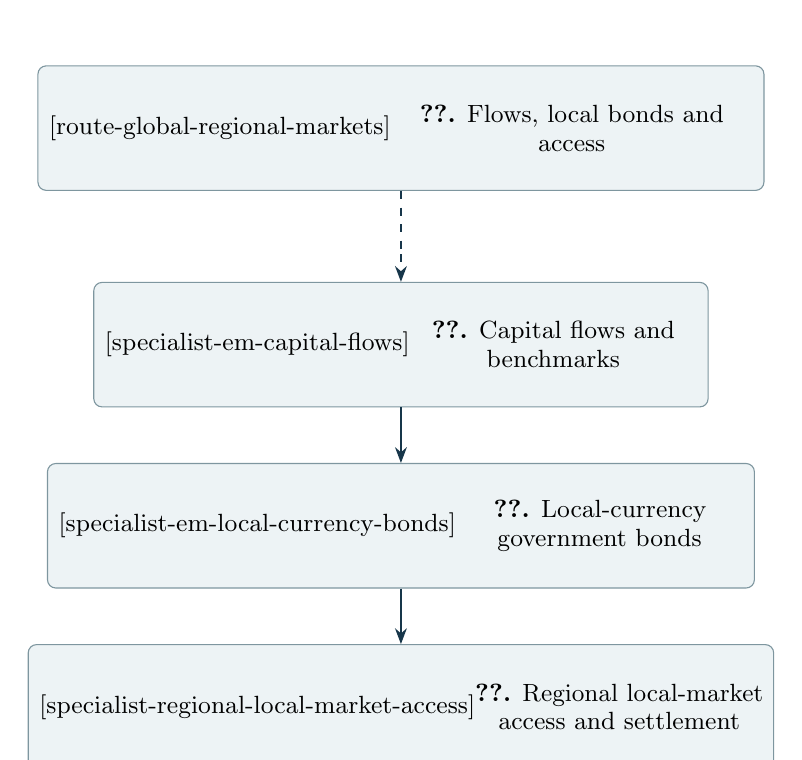
\begin{tikzpicture}[x=1cm,y=1cm]
\node[pathnode] (global-regional-markets) at (0.00,0) {\MeasurePathNode{4.6cm}{\textbf{\ref*{route-global-regional-markets}.} Flows, local bonds and access}\hyperref[route-global-regional-markets]{\parbox[c][\pathnodeheight][c]{4.6cm}{\centering \textbf{\ref*{route-global-regional-markets}.} Flows, local bonds and access}}};
\node[pathnode] (em-capital-flows) at (0.00,-2.75) {\MeasurePathNode{3.65cm}{\textbf{\ref*{specialist-em-capital-flows}.} Capital flows and benchmarks}\hyperref[specialist-em-capital-flows]{\parbox[c][\pathnodeheight][c]{3.65cm}{\centering \textbf{\ref*{specialist-em-capital-flows}.} Capital flows and benchmarks}}};
\node[pathnode] (em-local-currency-bonds) at (0.00,-5.05) {\MeasurePathNode{3.65cm}{\textbf{\ref*{specialist-em-local-currency-bonds}.} Local-currency government bonds}\hyperref[specialist-em-local-currency-bonds]{\parbox[c][\pathnodeheight][c]{3.65cm}{\centering \textbf{\ref*{specialist-em-local-currency-bonds}.} Local-currency government bonds}}};
\node[pathnode] (regional-local-market-access) at (0.00,-7.35) {\MeasurePathNode{3.65cm}{\textbf{\ref*{specialist-regional-local-market-access}.} Regional local-market access and settlement}\hyperref[specialist-regional-local-market-access]{\parbox[c][\pathnodeheight][c]{3.65cm}{\centering \textbf{\ref*{specialist-regional-local-market-access}.} Regional local-market access and settlement}}};
\draw[entryline] (global-regional-markets.south) -- (0.00,-1.60);
\draw[entryline] (0.00,-1.60) -- (0.00,-1.60);
\draw[entryarrow] (0.00,-1.60) -- (em-capital-flows.north);
\draw[patharrow] (em-capital-flows.south) -- (em-local-currency-bonds.north);
\draw[patharrow] (em-local-currency-bonds.south) -- (regional-local-market-access.north);
\end{tikzpicture}\end{center}
\textbf{Bring these foundations with you.}\begin{itemize}
\item \hyperref[specialist-em-currencies-intervention]{Emerging-market currencies: regimes, intervention and the global financial cycle} --- needed by \hyperref[specialist-em-capital-flows]{Capital flows and benchmarks}.
\item \hyperref[specialist-sovereign-municipal]{Sovereign default, restructuring and local-currency debt} --- needed by \hyperref[specialist-em-local-currency-bonds]{Local-currency government bonds}.
\end{itemize}\hyperref[learning-map]{Return to the whole-guide DAG.}
\Needspace{12\baselineskip}
\subsection{Capital flows, global investors and benchmark effects}\label{specialist-em-capital-flows}
\textbf{Specialist pathway.} In \hyperref[route-global-regional-markets]{Global and regional markets: capital flows, local bonds and market access}.

\textbf{Outcome.} Separate push from pull drivers of capital flows by type of flow; measure how fund investors, managers and benchmark rebalancing transmit shocks to emerging markets; estimate the price and currency effects of index-driven flows; and restate cross-border positions by nationality rather than residence.

\textbf{Prerequisites.} Global and regional markets overview; emerging-market currencies, intervention and the global financial cycle.

\textbf{Review first.} \hyperref[route-global-regional-markets]{Global and regional markets: capital flows, local bonds and market access}; \hyperref[specialist-em-currencies-intervention]{Emerging-market currencies: regimes, intervention and the global financial cycle}.

\textbf{Required readings, in order}
\begin{enumerate}\raggedright
\Needspace{5\baselineskip}\item \href{institutional_quantitative_finance_reading_list.pdf\#gr-forbes-warnock-2012}{Kristin J. Forbes and Francis E. Warnock, ``Capital flow waves: Surges, stops, flight, and retrenchment''}\CataloguePage{305}\NoteKey{gr-forbes-warnock-2012}\par \textbf{Evidence.} Identify surges, stops, flight and retrenchment from gross flows by foreigners and residents.
\Needspace{5\baselineskip}\item \href{institutional_quantitative_finance_reading_list.pdf\#gr-fratzscher-2012}{Marcel Fratzscher, ``Capital flows, push versus pull factors and the global financial crisis''}\CataloguePage{305}\NoteKey{gr-fratzscher-2012}\par \textbf{Evidence.} Compare push and pull factors in the 2008 collapse and the recovery of portfolio flows.
\Needspace{5\baselineskip}\item \href{institutional_quantitative_finance_reading_list.pdf\#gr-cerutti-claessens-puy-2019}{Eugenio Cerutti, Stijn Claessens and Damien Puy, ``Push factors and capital flows to emerging markets: why knowing your lender matters more than fundamentals''}\CataloguePage{305}\NoteKey{gr-cerutti-claessens-puy-2019}\par \textbf{Evidence.} See why the composition of a country's foreign investor base matters more than its fundamentals.
\Needspace{5\baselineskip}\item \href{institutional_quantitative_finance_reading_list.pdf\#gr-froot-oconnell-seasholes-2001}{Kenneth A. Froot, Paul G. J. O'Connell and Mark S. Seasholes, ``The portfolio flows of international investors''}\CataloguePage{306}\NoteKey{gr-froot-oconnell-seasholes-2001}\par \textbf{Data.} Study daily custodian flow data: persistence, trend-following and return forecasting.
\Needspace{5\baselineskip}\item \href{institutional_quantitative_finance_reading_list.pdf\#gr-griffin-nardari-stulz-2004}{John M. Griffin, Federico Nardari and Ren\'e M. Stulz, ``Are Daily Cross-Border Equity Flows Pushed or Pulled?''}\CataloguePage{306}\NoteKey{gr-griffin-nardari-stulz-2004}\par \textbf{Theory.} Model why daily equity flows chase local and world returns.
\Needspace{5\baselineskip}\item \href{institutional_quantitative_finance_reading_list.pdf\#gr-kaminsky-lyons-schmukler-2004}{Graciela Kaminsky, Richard K. Lyons and Sergio L. Schmukler, ``Managers, investors, and crises: mutual fund strategies in emerging markets''}\CataloguePage{306}\NoteKey{gr-kaminsky-lyons-schmukler-2004}\par \textbf{Evidence.} Separate momentum and contagion trading by fund managers and fund investors.
\Needspace{5\baselineskip}\item \href{institutional_quantitative_finance_reading_list.pdf\#gr-jotikasthira-lundblad-ramadorai-2012}{Chotibhak Jotikasthira, Christian Lundblad and Tarun Ramadorai, ``Asset Fire Sales and Purchases and the International Transmission of Funding Shocks''}\CataloguePage{306}\NoteKey{gr-jotikasthira-lundblad-ramadorai-2012}\par \textbf{Evidence.} Trace developed-market fund flows into emerging-market fire sales.
\Needspace{5\baselineskip}\item \href{institutional_quantitative_finance_reading_list.pdf\#gr-raddatz-schmukler-2012}{Claudio Raddatz and Sergio L. Schmukler, ``On the international transmission of shocks: Micro-evidence from mutual fund portfolios''}\CataloguePage{306}\NoteKey{gr-raddatz-schmukler-2012}\par \textbf{Evidence.} Decompose mutual-fund country allocations into investor flows and manager reallocation.
\Needspace{5\baselineskip}\item \href{institutional_quantitative_finance_reading_list.pdf\#gr-raddatz-schmukler-williams-2017}{Claudio Raddatz, Sergio L. Schmukler and Tom\'as Williams, ``International asset allocations and capital flows: The benchmark effect''}\CataloguePage{306}\NoteKey{gr-raddatz-schmukler-williams-2017}\par \textbf{Evidence.} Measure how much of country allocation benchmarks explain, even for active funds.
\Needspace{5\baselineskip}\item \href{institutional_quantitative_finance_reading_list.pdf\#gr-hau-massa-peress-2010}{Harald Hau, Massimo Massa and Joel Peress, ``Do Demand Curves for Currencies Slope Down? Evidence from the MSCI Global Index Change''}\CataloguePage{307}\NoteKey{gr-hau-massa-peress-2010}\par \textbf{Evidence.} Use the 2001--02 MSCI redefinition to show that index flows move currencies.
\Needspace{5\baselineskip}\item \href{institutional_quantitative_finance_reading_list.pdf\#gr-arslanalp-drakopoulos-goel-koepke-2020}{Serkan Arslanalp, Dimitris Drakopoulos, Rohit Goel and Robin Koepke, ``Benchmark-Driven Investments in Emerging Market Bond Markets: Taking Stock''}\CataloguePage{306}\NoteKey{gr-arslanalp-drakopoulos-goel-koepke-2020}\par \textbf{Mechanics.} Learn how EM bond indices are built and what benchmark-driven assets imply for flows.
\Needspace{5\baselineskip}\item \href{institutional_quantitative_finance_reading_list.pdf\#gr-chari-dilts-stedman-lundblad-2021}{Anusha Chari, Karlye Dilts Stedman and Christian Lundblad, ``Taper Tantrums: Quantitative Easing, Its Aftermath, and Emerging Market Capital Flows''}\CataloguePage{307}\NoteKey{gr-chari-dilts-stedman-lundblad-2021}\par \textbf{Evidence.} Trace US monetary policy shocks into the valuations and flows of US holdings of EM assets.
\Needspace{5\baselineskip}\item \href{institutional_quantitative_finance_reading_list.pdf\#gr-eichengreen-gupta-2015}{Barry Eichengreen and Poonam Gupta, ``Tapering talk: The impact of expectations of reduced Federal Reserve security purchases on emerging markets''}\CataloguePage{307}\NoteKey{gr-eichengreen-gupta-2015}\par \textbf{Evidence.} See which emerging markets the 2013 taper talk hit, and why.
\Needspace{5\baselineskip}\item \href{institutional_quantitative_finance_reading_list.pdf\#gr-coppola-maggiori-neiman-schreger-2021}{Antonio Coppola, Matteo Maggiori, Brent Neiman and Jesse Schreger, ``Redrawing the Map of Global Capital Flows: The Role of Cross-Border Financing and Tax Havens''}\CataloguePage{307}\NoteKey{gr-coppola-maggiori-neiman-schreger-2021}\par \textbf{Data.} Restate bilateral portfolio positions from tax-haven subsidiaries to their ultimate parents.
\end{enumerate}
\Needspace{5\baselineskip}\textbf{Checkpoint.} Assemble monthly balance-of-payments or fund-flow data for portfolio equity and bond flows to 15 emerging markets since 2005. Classify surge and stop episodes with the Forbes--Warnock method, regress flows on the VIX, US rates and the dollar, and compare the explained share for equity and bond flows. For one country, reconstruct its weight in a widely followed local-currency bond index around an inclusion or cap change, compute the flows implied by rebalancing for an assumed benchmarked asset base, and measure yield and currency moves in the implementation window against the announcement date.

\textbf{Optional branches.} \href{institutional_quantitative_finance_reading_list.pdf\#gr-koijen-yogo-2020}{Decompose exchange rates, yields and stock prices with a global demand system.}\BranchPage{307} \href{institutional_quantitative_finance_reading_list.pdf\#gr-jiang-richmond-zhang-2024}{Explain the US net foreign asset position with a portfolio approach.}\BranchPage{307} \href{institutional_quantitative_finance_reading_list.pdf\#depth-africa-imf-funding}{Compare Eurobond, syndicated-loan and local-currency financing in sub-Saharan Africa.}\BranchPage{313}
\par{\small \hyperref[learning-map]{Learning pathway DAG} \textbar{} \hyperref[route-global-regional-markets]{Section overview} \textbar{} \hyperref[map-global-regional-markets]{Section DAG}\NoteKey{em-capital-flows}}
\Needspace{12\baselineskip}
\subsection{Emerging-market local-currency government bonds: original sin, foreign holders and index inclusion}\label{specialist-em-local-currency-bonds}
\textbf{Specialist pathway.} In \hyperref[route-global-regional-markets]{Global and regional markets: capital flows, local bonds and market access}.

\textbf{Outcome.} Explain why emerging-market sovereigns moved from foreign- to local-currency borrowing and where currency mismatches went; decompose local-currency yields into credit, currency and duration risk; estimate the effects of foreign holdings and index rebalancing on yields, liquidity and volatility; and use investor-base data to assess flow risk.

\textbf{Prerequisites.} Capital flows, global investors and benchmark effects; sovereign default, restructuring and local-currency debt; covered interest parity and the cross-currency basis.

\textbf{Review first.} \hyperref[route-global-regional-markets]{Global and regional markets: capital flows, local bonds and market access}; \hyperref[specialist-em-capital-flows]{Capital flows, global investors and benchmark effects}; \hyperref[specialist-sovereign-municipal]{Sovereign default, restructuring and local-currency debt}.

\textbf{Required readings, in order}
\begin{enumerate}\raggedright
\Needspace{5\baselineskip}\item \href{institutional_quantitative_finance_reading_list.pdf\#gr-hausmann-panizza-2003}{Ricardo Hausmann and Ugo Panizza, ``On the determinants of Original Sin: an empirical investigation''}\CataloguePage{308}\NoteKey{gr-hausmann-panizza-2003}\par \textbf{Evidence.} Measure original sin and test which country traits explain it.
\Needspace{5\baselineskip}\item \href{institutional_quantitative_finance_reading_list.pdf\#gr-claessens-klingebiel-schmukler-2007}{Stijn Claessens, Daniela Klingebiel and Sergio L. Schmukler, ``Government Bonds in Domestic and Foreign Currency: the Role of Institutional and Macroeconomic Factors''}\CataloguePage{308}\NoteKey{gr-claessens-klingebiel-schmukler-2007}\par \textbf{Evidence.} Relate the depth and currency composition of government bond markets to domestic investor bases and institutions.
\Needspace{5\baselineskip}\item \href{institutional_quantitative_finance_reading_list.pdf\#gr-burger-warnock-2007}{John D. Burger and Francis E. Warnock, ``Foreign participation in local currency bond markets''}\CataloguePage{308}\NoteKey{gr-burger-warnock-2007}\par \textbf{Evidence.} See why foreign investors avoid volatile, negatively skewed local bond markets.
\Needspace{5\baselineskip}\item \href{institutional_quantitative_finance_reading_list.pdf\#gr-burger-warnock-warnock-2012}{John D. Burger, Francis E. Warnock and Veronica Cacdac Warnock, ``Emerging Local Currency Bond Markets''}\CataloguePage{308}\NoteKey{gr-burger-warnock-warnock-2012}\par \textbf{Evidence.} Track the growth of EM local bond markets and US investors' allocations to them.
\Needspace{5\baselineskip}\item \href{institutional_quantitative_finance_reading_list.pdf\#gr-eichengreen-hausmann-panizza-2023}{Barry Eichengreen, Ricardo Hausmann and Ugo Panizza, ``Yet it Endures: The Persistence of Original Sin''}\CataloguePage{308}\NoteKey{gr-eichengreen-hausmann-panizza-2023}\par \textbf{Evidence.} See currency mismatches move from sovereigns to domestic hedgers rather than disappear.
\Needspace{5\baselineskip}\item \href{institutional_quantitative_finance_reading_list.pdf\#gr-onen-shin-von-peter-2025}{Mert Onen, Hyun Song Shin and Goetz von Peter, ``Overcoming original sin: Shedding new light on uneven progress''}\CataloguePage{309}\NoteKey{gr-onen-shin-von-peter-2025}\par \textbf{Data.} Measure progress against original sin by country and issuer with a new dataset.
\Needspace{5\baselineskip}\item \href{institutional_quantitative_finance_reading_list.pdf\#gr-gadanecz-miyajima-shu-2018}{Blaise Gadanecz, Ken Miyajima and Chang Shu, ``Emerging market local currency sovereign bond yields: The role of exchange rate risk''}\CataloguePage{309}\NoteKey{gr-gadanecz-miyajima-shu-2018}\par \textbf{Evidence.} Measure how exchange-rate volatility and expected depreciation raise local-currency yields.
\Needspace{5\baselineskip}\item \href{institutional_quantitative_finance_reading_list.pdf\#gr-bertaut-bruno-shin-2025}{Carol Bertaut, Valentina Bruno and Hyun Song Shin, ``Original Sin Redux: Role of Duration Risk''}\CataloguePage{309}\NoteKey{gr-bertaut-bruno-shin-2025}\par \textbf{Evidence.} See how duration and currency risk interact in US investors' flows into local bonds.
\Needspace{5\baselineskip}\item \href{institutional_quantitative_finance_reading_list.pdf\#gr-peiris-2010}{Shanaka J. Peiris, ``Foreign Participation in Emerging Markets' Local Currency Bond Markets''}\CataloguePage{309}\NoteKey{gr-peiris-2010}\par \textbf{Evidence.} Estimate how foreign participation lowered long-term local yields in 2000--09.
\Needspace{5\baselineskip}\item \href{institutional_quantitative_finance_reading_list.pdf\#gr-ebeke-lu-2015}{Christian Ebeke and Yinqiu Lu, ``Emerging market local currency bond yields and foreign holdings -- A fortune or misfortune?''}\CataloguePage{309}\NoteKey{gr-ebeke-lu-2015}\par \textbf{Evidence.} Use an instrument for foreign holdings to estimate effects on yields and volatility after 2008.
\Needspace{5\baselineskip}\item \href{institutional_quantitative_finance_reading_list.pdf\#gr-arslanalp-tsuda-2014}{Serkan Arslanalp and Takahiro Tsuda, ``Tracking Global Demand for Emerging Market Sovereign Debt''}\CataloguePage{309}\NoteKey{gr-arslanalp-tsuda-2014}\par \textbf{Data.} Track foreign holdings of EM government debt by investor type.
\Needspace{5\baselineskip}\item \href{institutional_quantitative_finance_reading_list.pdf\#gr-fang-hardy-lewis-2022}{Xiang Fang, Bryan Hardy and Karen K. Lewis, ``Who Holds Sovereign Debt and Why It Matters''}\CataloguePage{310}\NoteKey{gr-fang-hardy-lewis-2022}\par \textbf{Evidence.} Estimate how investor composition, especially non-bank demand, sets the cost of sovereign debt.
\Needspace{5\baselineskip}\item \href{institutional_quantitative_finance_reading_list.pdf\#gr-pandolfi-williams-2019}{Lorenzo Pandolfi and Tomas Williams, ``Capital flows and sovereign debt markets: Evidence from index rebalancings''}\CataloguePage{309}\NoteKey{gr-pandolfi-williams-2019}\par \textbf{Evidence.} Use index rebalancing as an exogenous flow to measure price, depth and currency effects.
\Needspace{5\baselineskip}\item \href{institutional_quantitative_finance_reading_list.pdf\#depth-eme-liquidity}{Bernardus Doornik, Jon Frost, Rafael Guerra, Alexandre Tombini and Christian Upper, Towards Liquid and Resilient Government Debt Markets in EMEs}\CataloguePage{308}\NoteKey{depth-eme-liquidity}\par \textbf{Evidence.} Identify the empirical limits of emerging-market government bond liquidity measures.
\Needspace{5\baselineskip}\item \href{institutional_quantitative_finance_reading_list.pdf\#gr-amstad-he-2020}{Marlene Amstad and Zhiguo He, ``Chinese Bond Markets and Interbank Market''}\CataloguePage{317}\NoteKey{gr-amstad-he-2020}\par \textbf{Mechanics.} Map China's segmented interbank and exchange bond markets, their regulators and ratings.
\end{enumerate}
\Needspace{5\baselineskip}\textbf{Checkpoint.} For Brazil, Mexico, Indonesia, South Africa and Poland, decompose five-year local-currency yields into the US Treasury yield, the CIP-implied currency premium and the residual local-currency credit spread. Merge foreign-holder shares by investor type and index weights, estimate how foreign holdings relate to yield levels and volatility, and run an event study of yields, bid--ask spreads and the currency around index rebalancing dates. Report hedged and unhedged dollar returns separately and mark gaps in the holder data.

\textbf{Optional branches.} \href{institutional_quantitative_finance_reading_list.pdf\#rt-hss-em-premia-2020}{Link currency depreciation to wider local-currency bond spreads.}\BranchPage{231} \href{institutional_quantitative_finance_reading_list.pdf\#gr-miyajima-mohanty-chan-2015}{Check how far domestic factors anchor local yields.}\BranchPage{309} \href{institutional_quantitative_finance_reading_list.pdf\#gr-geng-pan-2024}{Price government support and the SOE premium in China's credit market.}\BranchPage{317} \href{institutional_quantitative_finance_reading_list.pdf\#gr-ding-xiong-zhang-2022}{See why China's corporate debt is issued overpriced.}\BranchPage{317} \href{institutional_quantitative_finance_reading_list.pdf\#depth-latam-idb-flows}{Test whether foreign holders stabilise Latin American local-currency bond markets.}\BranchPage{308} \href{institutional_quantitative_finance_reading_list.pdf\#depth-asean-lct}{Compare ASEAN local-currency frameworks and Malaysian hedging permissions.}\BranchPage{312} \href{institutional_quantitative_finance_reading_list.pdf\#depth-gcc-imf-bonds}{Compare GCC international issuance with uneven local bond and repo markets.}\BranchPage{314} \href{institutional_quantitative_finance_reading_list.pdf\#depth-india-premia}{Relate Indian term and credit premia to liquidity and macro variables.}\BranchPage{312}
\par{\small \hyperref[learning-map]{Learning pathway DAG} \textbar{} \hyperref[route-global-regional-markets]{Section overview} \textbar{} \hyperref[map-global-regional-markets]{Section DAG}\NoteKey{em-local-currency-bonds}}
\Needspace{12\baselineskip}
\subsection{Regional local-market access and settlement}\label{specialist-regional-local-market-access}
\textbf{Specialist pathway.} In \hyperref[route-global-regional-markets]{Global and regional markets: capital flows, local bonds and market access}.

\textbf{Outcome.} Trace a local-currency security from eligibility and beneficial ownership through execution, custody, settlement, tax, FX hedge and repatriation in dated jurisdiction-specific rules.

\textbf{Prerequisites.} Emerging-market local-currency government bonds; sovereign bonds, FX forwards, market microstructure and transaction-cost accounting.

\textbf{Review first.} \hyperref[route-global-regional-markets]{Global and regional markets: capital flows, local bonds and market access}; \hyperref[specialist-em-local-currency-bonds]{Emerging-market local-currency government bonds: original sin, foreign holders and index inclusion}.

\textbf{Required readings, in order}
\begin{enumerate}\raggedright
\Needspace{5\baselineskip}\item \href{institutional_quantitative_finance_reading_list.pdf\#gap-sovereign-local-currency}{Wenxin Du and Jesse Schreger, Local Currency Sovereign Risk}\CataloguePage{229}\NoteKey{gap-sovereign-local-currency}\par \textbf{Mechanics.} Separate local-currency sovereign risk from hard-currency credit and investor FX risk.
\Needspace{5\baselineskip}\item \href{institutional_quantitative_finance_reading_list.pdf\#gr-msci-gmar-2026}{MSCI, 2026 Global Market Accessibility Review}\CataloguePage{315}\NoteKey{gr-msci-gmar-2026}\par \textbf{Mechanics.} Score market access on MSCI's 18 measures: ownership limits, capital flows, registration, settlement, custody, transferability and data.
\Needspace{5\baselineskip}\item \href{institutional_quantitative_finance_reading_list.pdf\#gap-cip}{Wenxin Du, Alexander Tepper and Adrien Verdelhan, Deviations from Covered Interest Rate Parity}\CataloguePage{282}\NoteKey{gap-cip}\par \textbf{Valuation.} Frame covered-interest-parity and FX funding basis before assuming a hedge is executable.
\Needspace{5\baselineskip}\item \href{institutional_quantitative_finance_reading_list.pdf\#depth-india-far}{Reserve Bank of India, Fully Accessible Route: Exclusion of New 14- and 30-Year Securities; Sovereign Green Bond Trading and Settlement Scheme}\CataloguePage{311}\NoteKey{depth-india-far}\par \textbf{Mechanics.} Use one documented foreign-investor bond eligibility regime as a case.
\Needspace{5\baselineskip}\item \href{institutional_quantitative_finance_reading_list.pdf\#depth-india-rbi-settlement}{Reserve Bank of India Working Group, Report on Comprehensive Review of Trading and Settlement Timings of Markets Regulated by the Reserve Bank; Clearing Corporation of India, Daily Data, MTM Prices}\CataloguePage{311}\NoteKey{depth-india-rbi-settlement}\par \textbf{Implementation.} Map the India trading and settlement chain, not just the eligible security list.
\Needspace{5\baselineskip}\item \href{institutional_quantitative_finance_reading_list.pdf\#evidence-india-april-sequence}{Reserve Bank of India, A.P. (DIR) 24, A.P. (DIR) 03 (revised) and A.P. (DIR) 07}\CataloguePage{311}\NoteKey{evidence-india-april-sequence}\par \textbf{Implementation.} Apply a dated circular sequence rather than a timeless India-access summary.
\Needspace{5\baselineskip}\item \href{institutional_quantitative_finance_reading_list.pdf\#evidence-kenya-access}{Central Bank of Kenya, government-bond settlement guidelines; Clearstream, Kenya link announcement and market link guide}\CataloguePage{313}\NoteKey{evidence-kenya-access}\par \textbf{Mechanics.} Compare account, registration and investor-access rules in a second market.
\Needspace{5\baselineskip}\item \href{institutional_quantitative_finance_reading_list.pdf\#evidence-kenya-instruments}{Central Bank of Kenya, September 2026 bond reopening prospectus, yield-curve methodology and Kenya FX Code}\CataloguePage{313}\NoteKey{evidence-kenya-instruments}\par \textbf{Data.} Connect eligible instruments to dated market and security data.
\Needspace{5\baselineskip}\item \href{institutional_quantitative_finance_reading_list.pdf\#evidence-nigeria-instruments}{Debt Management Office Nigeria, FGN bond access guide; 2024 domestic USD bond offer and institutional subscription form}\CataloguePage{313}\NoteKey{evidence-nigeria-instruments}\par \textbf{Data.} Examine local instrument and market-data availability in a third case.
\Needspace{5\baselineskip}\item \href{institutional_quantitative_finance_reading_list.pdf\#evidence-nigeria-hedges}{FMDQ Exchange, OTC FX Futures Market Operational Standards and cleared naira-settled NDF documentation}\CataloguePage{314}\NoteKey{evidence-nigeria-hedges}\par \textbf{Implementation.} Test the actual FX hedge and convertibility terms for Nigeria rather than assuming an offshore forward.
\Needspace{5\baselineskip}\item \href{institutional_quantitative_finance_reading_list.pdf\#depth-asean-adb-bonds}{Asian Development Bank ASEAN+3 Bond Market Forum, Bond Market Guides for Indonesia and Thailand; ADB, Local Currency Bond Markets, Foreign Investor Participation, and Capital Flow Volatility in Emerging Asia}\CataloguePage{312}\NoteKey{depth-asean-adb-bonds}\par \textbf{Evidence.} Place the cases in a regional bond-market-depth comparison.
\Needspace{5\baselineskip}\item \href{institutional_quantitative_finance_reading_list.pdf\#gr-eu-t1-regulation-2025}{European Parliament and Council of the European Union, Regulation (EU) 2025/2075 amending Regulation (EU) No 909/2014 as regards a shorter settlement cycle in the Union}\CataloguePage{315}\NoteKey{gr-eu-t1-regulation-2025}\par \textbf{Implementation.} Plan for EU on-venue settlement at T+1 from 11 October 2027, with its exemptions.
\Needspace{5\baselineskip}\item \href{institutional_quantitative_finance_reading_list.pdf\#gr-eu-faster-directive-2024}{Council of the European Union, Council Directive (EU) 2025/50 of 10 December 2024 on faster and safer relief of excess withholding taxes (FASTER)}\CataloguePage{315}\NoteKey{gr-eu-faster-directive-2024}\par \textbf{Implementation.} Track EU withholding-tax relief at source, quick refunds and digital residence certificates from 2030.
\end{enumerate}
\Needspace{5\baselineskip}\textbf{Checkpoint.} Choose two of India, Kenya and Nigeria and a dated local bond in each, and first score each market on MSCI's accessibility measures. Prepare an investor-to-custodian execution sheet: eligibility and account opening, security identifier, quote source, lot/auction rules, trade date, CSD and cash settlement, withholding-tax relief route and uncertainty, hedge eligibility and tenor, conversion/repatriation, holidays and all-in hedged yield. Attach the operative circular/version for every rule, run a failed settlement and FX-roll scenario, and leave any missing executable quote or legal permission explicitly unresolved.

\textbf{Optional branches.} \href{institutional_quantitative_finance_reading_list.pdf\#depth-china-bond-connect}{Extend the checklist to an access channel with a different custody and nominee architecture.}\BranchPage{311} \href{institutional_quantitative_finance_reading_list.pdf\#depth-saudi-local-sukuk}{Extend to Saudi local sukuk and investor eligibility.}\BranchPage{314} \href{institutional_quantitative_finance_reading_list.pdf\#depth-latam-banxico-data}{Add a Mexico market-data case.}\BranchPage{312} \href{institutional_quantitative_finance_reading_list.pdf\#depth-indonesia-srbi}{Compare central-bank bills and access in Indonesia.}\BranchPage{312} \href{institutional_quantitative_finance_reading_list.pdf\#exp-tplusone}{Compare the US move to T+1 and the readiness issues examiners found.}\BranchPage{539} \href{institutional_quantitative_finance_reading_list.pdf\#evidence-india-june-exclusions}{Follow a later dated RBI change to swap and open-position rules.}\BranchPage{312} \href{institutional_quantitative_finance_reading_list.pdf\#evidence-nigeria-research}{Relate Nigerian policy rates, bill yields and exchange-rate pass-through.}\BranchPage{314} \href{institutional_quantitative_finance_reading_list.pdf\#evidence-kenya-empirical}{Read a historical account of Kenyan yield-curve shifts before modelling the curve.}\BranchPage{313} \href{institutional_quantitative_finance_reading_list.pdf\#depth-uae-money-market}{Compare UAE central-bank bills, EIBOR and dollar funding.}\BranchPage{314}
\par{\small \hyperref[learning-map]{Learning pathway DAG} \textbar{} \hyperref[route-global-regional-markets]{Section overview} \textbar{} \hyperref[map-global-regional-markets]{Section DAG}\NoteKey{regional-local-market-access}}
\clearpage
\part{Portfolio financing and execution}\label{part-portfolio-financing-execution}
Build and evaluate portfolios, connect them to funding, collateral and liabilities, then study market microstructure and the cost of executing orders across asset classes.

\textbf{Sections in learning order}\begin{enumerate}
\item[\ref*{route-portfolio-construction-risk}.] \hyperref[route-portfolio-construction-risk]{Portfolio construction and risk} --- Turn forecasts into constrained portfolios, measure tail and systemic risk, then evaluate managers and climate exposure.
\item[\ref*{route-portfolio-risk-financing}.] \hyperref[route-portfolio-risk-financing]{Funding, collateral and liquidity} --- Start with funding and crowding, money markets and secured financing, collateral risk and asset-liability management, then combine financing and collateral risk in CFDs and total return swaps.
\item[\ref*{route-execution-market-making}.] \hyperref[route-execution-market-making]{Market microstructure and market making} --- Study order-book mechanics and market making, then order-book learning, options market making, dealer market making in bonds and swaps, and simulation; FX dealing builds on bond and swap dealing, and high-frequency trading is a separate entry point. Crypto venues apply the same tools in Part VI.
\item[\ref*{route-execution-trading-costs}.] \hyperref[route-execution-trading-costs]{Execution, trading costs and market structure} --- Start with price impact and transaction-cost analysis, the rules that shape execution quality, and dealer-market bonds and FX; then execution around ETFs and index events and in futures, which build on price impact, and retail CFD markets, which build on the rules.
\end{enumerate}
\hyperref[learning-map]{Return to the learning pathway DAG.}
\clearpage
\section{Portfolio construction and risk}\label{route-portfolio-construction-risk}
\label{route-19}
\textbf{Learning sequence.} Turn forecasts into constrained portfolios, measure tail and systemic risk, then evaluate managers and climate exposure.

\textbf{Section goals.} Across its pathways, this section teaches you to:
\begin{itemize}[leftmargin=1.4em,itemsep=0pt,topsep=1pt]
\item construct constrained portfolios with factor risk models, shrinkage and costs (\hyperref[specialist-portfolio-construction]{\ref*{specialist-portfolio-construction}})
\item forecast and backtest VaR and expected shortfall, design tail hedges and run systemic stress tests (\hyperref[specialist-risk-tail-systemic]{\ref*{specialist-risk-tail-systemic}})
\item attribute returns and separate manager skill from luck (\hyperref[specialist-performance-manager-evaluation]{\ref*{specialist-performance-manager-evaluation}})
\item measure climate exposure and test carbon and green premia (\hyperref[specialist-climate-sustainable]{\ref*{specialist-climate-sustainable}})
\end{itemize}
\textbf{Overview outcome.} Construct and evaluate a portfolio whose forecasts, risk model, constraints, costs and tail measures are explicit and testable.

\textbf{Prerequisites.} Common toolkit; portfolio exposure, covariance estimation and basic optimisation.

\textbf{Review first.} \hyperref[route-common-toolkit]{Common toolkit}.

\textbf{Required readings, in order}
\begin{enumerate}\raggedright
\Needspace{5\baselineskip}\item \href{institutional_quantitative_finance_reading_list.pdf\#s7-meucci}{Attilio Meucci, \emph{Risk and Asset Allocation}}\CataloguePage{106}\NoteKey{s7-meucci}\par Express exposure and risk in a consistent multi-asset portfolio language.
\Needspace{5\baselineskip}\item \href{institutional_quantitative_finance_reading_list.pdf\#alpha-grinold}{Richard C. Grinold and Ronald N. Kahn, \emph{Active Portfolio Management}}\CataloguePage{93}\NoteKey{alpha-grinold}\par Relate forecasts, breadth, risk models and constraints in an active portfolio; treat the fundamental law as an approximation when signals and costs are correlated.
\Needspace{5\baselineskip}\item \href{institutional_quantitative_finance_reading_list.pdf\#s7-qrm}{Alexander McNeil, Rüdiger Frey and Paul Embrechts, \emph{Quantitative Risk Management}}\CataloguePage{102}\NoteKey{s7-qrm}\par Measure tails and dependence without treating a fitted distribution as a stress guarantee.
\end{enumerate}
\Needspace{5\baselineskip}\textbf{Checkpoint.} Build a long-only and a long-short portfolio from the same forecasts and risk model. Report ex-ante and realised risk, turnover, costs and the largest tail-loss contributors; rerun with a shrunk covariance estimate and explain which decisions changed.

\textbf{Optional branches.} \href{institutional_quantitative_finance_reading_list.pdf\#latest-palomar-portfolio}{Use the computational portfolio text for formulation, constraints and numerical comparisons.}\BranchPage{94} \href{institutional_quantitative_finance_reading_list.pdf\#latest-complex-modern-portfolio-theory}{Examine recent high-dimensional estimation claims alongside the existing risk and cost foundations.}\BranchPage{93}
\par\textbf{Continue in this section.} \hyperref[specialist-portfolio-construction]{Portfolio construction, estimation error and risk models}; \hyperref[specialist-risk-tail-systemic]{Market risk, tail hedging and systemic stress}; \hyperref[specialist-performance-manager-evaluation]{Performance attribution and manager evaluation}; \hyperref[specialist-climate-sustainable]{Climate risk and sustainable portfolios}.
\par{\small \hyperref[learning-map]{Learning pathway DAG} \textbar{} \hyperref[map-portfolio-construction-risk]{Section DAG}\NoteKey{portfolio-construction-risk}}
\clearpage
\subsection*{Portfolio construction and risk: pathway DAG}\phantomsection\label{map-portfolio-construction-risk}
\addcontentsline{toc}{subsection}{Portfolio construction and risk: pathway DAG}
Start with the section overview's readings, for orientation. Solid arrows show prerequisites within this section. Dashed connectors identify entry points with no further prerequisite in this section; the linked foundations below still apply. Follow the arrows for dependencies and the subsection numbers for reading order. Every node is clickable.
\begin{center}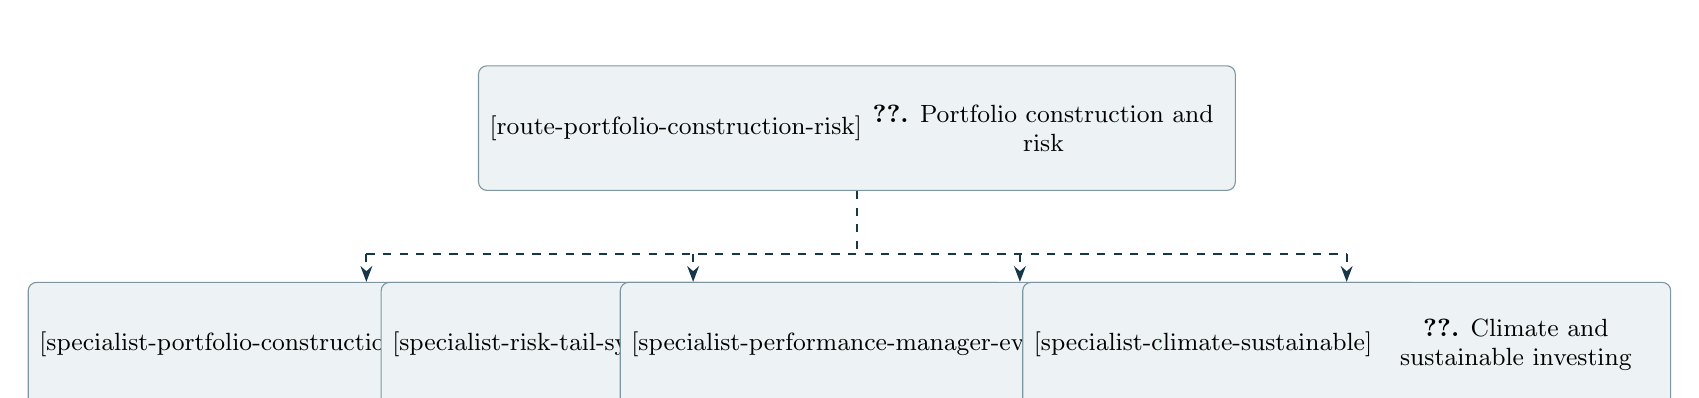
\begin{tikzpicture}[x=1cm,y=1cm]
\node[pathnode] (portfolio-construction-risk) at (6.23,0) {\MeasurePathNode{4.6cm}{\textbf{\ref*{route-portfolio-construction-risk}.} Portfolio construction and risk}\hyperref[route-portfolio-construction-risk]{\parbox[c][\pathnodeheight][c]{4.6cm}{\centering \textbf{\ref*{route-portfolio-construction-risk}.} Portfolio construction and risk}}};
\node[pathnode] (portfolio-construction) at (0.00,-2.75) {\MeasurePathNode{3.65cm}{\textbf{\ref*{specialist-portfolio-construction}.} Portfolio construction}\hyperref[specialist-portfolio-construction]{\parbox[c][\pathnodeheight][c]{3.65cm}{\centering \textbf{\ref*{specialist-portfolio-construction}.} Portfolio construction}}};
\node[pathnode] (risk-tail-systemic) at (4.15,-2.75) {\MeasurePathNode{3.65cm}{\textbf{\ref*{specialist-risk-tail-systemic}.} Tail and systemic risk}\hyperref[specialist-risk-tail-systemic]{\parbox[c][\pathnodeheight][c]{3.65cm}{\centering \textbf{\ref*{specialist-risk-tail-systemic}.} Tail and systemic risk}}};
\node[pathnode] (performance-manager-evaluation) at (8.30,-2.75) {\MeasurePathNode{3.65cm}{\textbf{\ref*{specialist-performance-manager-evaluation}.} Performance and manager evaluation}\hyperref[specialist-performance-manager-evaluation]{\parbox[c][\pathnodeheight][c]{3.65cm}{\centering \textbf{\ref*{specialist-performance-manager-evaluation}.} Performance and manager evaluation}}};
\node[pathnode] (climate-sustainable) at (12.45,-2.75) {\MeasurePathNode{3.65cm}{\textbf{\ref*{specialist-climate-sustainable}.} Climate and sustainable investing}\hyperref[specialist-climate-sustainable]{\parbox[c][\pathnodeheight][c]{3.65cm}{\centering \textbf{\ref*{specialist-climate-sustainable}.} Climate and sustainable investing}}};
\draw[entryline] (portfolio-construction-risk.south) -- (6.23,-1.60);
\draw[entryline] (0.00,-1.60) -- (12.45,-1.60);
\draw[entryarrow] (0.00,-1.60) -- (portfolio-construction.north);
\draw[entryarrow] (4.15,-1.60) -- (risk-tail-systemic.north);
\draw[entryarrow] (8.30,-1.60) -- (performance-manager-evaluation.north);
\draw[entryarrow] (12.45,-1.60) -- (climate-sustainable.north);
\end{tikzpicture}\end{center}
\textbf{Bring these foundations with you.}\begin{itemize}
\item \hyperref[specialist-high-dimensional-estimation]{High-dimensional estimation, random matrices and heavy tails} --- needed by \hyperref[specialist-portfolio-construction]{Portfolio construction}, \hyperref[specialist-risk-tail-systemic]{Tail and systemic risk}.
\item \hyperref[specialist-backtest-inference]{Backtest inference, multiple testing and Sharpe-ratio statistics} --- needed by \hyperref[specialist-performance-manager-evaluation]{Performance and manager evaluation}.
\item \hyperref[specialist-empirical-asset-pricing]{Empirical asset pricing: factor models and tests} --- needed by \hyperref[specialist-climate-sustainable]{Climate and sustainable investing}.
\end{itemize}\hyperref[learning-map]{Return to the whole-guide DAG.}
\Needspace{12\baselineskip}
\subsection{Portfolio construction, estimation error and risk models}\label{specialist-portfolio-construction}
\textbf{Specialist pathway.} In \hyperref[route-portfolio-construction-risk]{Portfolio construction and risk}.

\textbf{Outcome.} Construct a constrained portfolio from noisy forecasts with a factor risk model, shrinkage and costs, and attribute its realised risk.

\textbf{Prerequisites.} Portfolio construction and risk overview; high-dimensional estimation.

\textbf{Review first.} \hyperref[route-portfolio-construction-risk]{Portfolio construction and risk}; \hyperref[specialist-high-dimensional-estimation]{High-dimensional estimation, random matrices and heavy tails}.

\textbf{Required readings, in order}
\begin{enumerate}\raggedright
\Needspace{5\baselineskip}\item \href{institutional_quantitative_finance_reading_list.pdf\#s6-markowitz}{Harry Markowitz, ``Portfolio Selection''}\CataloguePage{93}\NoteKey{s6-markowitz}\par \textbf{Foundations.} Start from mean-variance selection.
\Needspace{5\baselineskip}\item \href{institutional_quantitative_finance_reading_list.pdf\#wide-michaud-enigma}{Richard O. Michaud, ``The Markowitz Optimization Enigma: Is "Optimized" Optimal?''}\CataloguePage{95}\NoteKey{wide-michaud-enigma}\par \textbf{Evidence.} See optimisers maximise estimation error.
\Needspace{5\baselineskip}\item \href{institutional_quantitative_finance_reading_list.pdf\#wide-chopra-ziemba}{Vijay K. Chopra and William T. Ziemba, ``The Effect of Errors in Means, Variances, and Covariances on Optimal Portfolio Choice''}\CataloguePage{95}\NoteKey{wide-chopra-ziemba}\par \textbf{Evidence.} Rank the cost of errors in means, variances and covariances.
\Needspace{5\baselineskip}\item \href{institutional_quantitative_finance_reading_list.pdf\#wide-kan-zhou}{Raymond Kan and Guofu Zhou, ``Optimal Portfolio Choice with Parameter Uncertainty''}\CataloguePage{95}\NoteKey{wide-kan-zhou}\par \textbf{Theory.} Quantify utility loss from parameter uncertainty.
\Needspace{5\baselineskip}\item \href{institutional_quantitative_finance_reading_list.pdf\#s7-demiguel}{Victor DeMiguel, Lorenzo Garlappi and Raman Uppal, ``Optimal Versus Naive Diversification''}\CataloguePage{93}\NoteKey{s7-demiguel}\par \textbf{Counter-evidence.} Compare with naive diversification.
\Needspace{5\baselineskip}\item \href{institutional_quantitative_finance_reading_list.pdf\#wide-ledoit-wolf-review}{Olivier Ledoit and Michael Wolf, ``The Power of (Non-)Linear Shrinking: A Review and Guide to Covariance Matrix Estimation''}\CataloguePage{97}\NoteKey{wide-ledoit-wolf-review}\par \textbf{Methods.} Choose a covariance shrinkage estimator.
\Needspace{5\baselineskip}\item \href{institutional_quantitative_finance_reading_list.pdf\#wide-connor-goldberg-korajczyk}{Gregory Connor, Lisa R. Goldberg and Robert A. Korajczyk, \emph{Portfolio Risk Analysis}}\CataloguePage{97}\NoteKey{wide-connor-goldberg-korajczyk}\par \textbf{Methods.} Build and evaluate factor risk models.
\Needspace{5\baselineskip}\item \href{institutional_quantitative_finance_reading_list.pdf\#wide-demiguel-norm}{Victor DeMiguel, Lorenzo Garlappi, Francisco J. Nogales and Raman Uppal, ``A Generalized Approach to Portfolio Optimization: Improving Performance by Constraining Portfolio Norms''}\CataloguePage{95}\NoteKey{wide-demiguel-norm}\par \textbf{Methods.} Constrain portfolio norms.
\Needspace{5\baselineskip}\item \href{institutional_quantitative_finance_reading_list.pdf\#alpha-black}{Fischer Black and Robert Litterman, ``Global Portfolio Optimization''}\CataloguePage{93}\NoteKey{alpha-black}\par \textbf{Methods.} Blend views with equilibrium returns.
\Needspace{5\baselineskip}\item \href{institutional_quantitative_finance_reading_list.pdf\#wide-maillard-roncalli-erc}{Sébastien Maillard, Thierry Roncalli and Jérôme Teïletche, ``The Properties of Equally Weighted Risk Contribution Portfolios''}\CataloguePage{98}\NoteKey{wide-maillard-roncalli-erc}\par \textbf{Methods.} Construct equal-risk-contribution portfolios.
\Needspace{5\baselineskip}\item \href{institutional_quantitative_finance_reading_list.pdf\#wide-lopez-de-prado-hrp}{Marcos López de Prado, ``Building Diversified Portfolios that Outperform Out of Sample''}\CataloguePage{98}\NoteKey{wide-lopez-de-prado-hrp}\par \textbf{Methods.} Allocate hierarchically without inversion.
\Needspace{5\baselineskip}\item \href{institutional_quantitative_finance_reading_list.pdf\#wide-clarke-transfer-coefficient}{Roger Clarke, Harindra de Silva and Steven Thorley, ``Portfolio Constraints and the Fundamental Law of Active Management''}\CataloguePage{96}\NoteKey{wide-clarke-transfer-coefficient}\par \textbf{Implementation.} Measure constraint drag with the transfer coefficient.
\Needspace{5\baselineskip}\item \href{institutional_quantitative_finance_reading_list.pdf\#wide-boyd-markowitz-seventy}{Stephen Boyd, Kasper Johansson, Ronald Kahn, Philipp Schiele and Thomas Schmelzer, ``Markowitz Portfolio Construction at Seventy''}\CataloguePage{95}\NoteKey{wide-boyd-markowitz-seventy}\par \textbf{Implementation.} Formulate a modern convex Markowitz problem with costs.
\Needspace{5\baselineskip}\item \href{institutional_quantitative_finance_reading_list.pdf\#exp-boyd-multiperiod-trading}{Stephen Boyd, Enzo Busseti, Steven Diamond, Ronald N. Kahn, Kwangmoo Koh, Peter Nystrup, and Jan Speth, Multi-Period Trading via Convex Optimization}\CataloguePage{99}\NoteKey{exp-boyd-multiperiod-trading}\par \textbf{Implementation.} Extend to multi-period trading.
\Needspace{5\baselineskip}\item \href{institutional_quantitative_finance_reading_list.pdf\#w3-kelly-upsa}{Bryan Kelly, Semyon Malamud, Mo Pourmohammadi and Fabio Trojani, ``Universal Portfolio Shrinkage''}\CataloguePage{96}\NoteKey{w3-kelly-upsa}\par \textbf{Methods.} Shrink covariance for portfolio objectives with UPSA.
\end{enumerate}
\Needspace{5\baselineskip}\textbf{Checkpoint.} For a 500-stock universe and a noisy alpha signal, build mean-variance portfolios with sample, shrunk and factor-model covariances, plus ERC and HRP; backtest with costs, report ex-ante versus realised risk, transfer coefficients and turnover.

\textbf{Optional branches.} \href{institutional_quantitative_finance_reading_list.pdf\#wide-meucci-flexible-views}{Blend arbitrary views with entropy pooling.}\BranchPage{98} \href{institutional_quantitative_finance_reading_list.pdf\#wide-paleologo-elements}{Read a practitioner portfolio-and-risk text.}\BranchPage{95} \href{institutional_quantitative_finance_reading_list.pdf\#wide-cvxportfolio}{Implement multi-period optimisation in code.}\BranchPage{524} \href{institutional_quantitative_finance_reading_list.pdf\#w2-davis-norman}{Derive no-trade regions under costs.}\BranchPage{100} \href{institutional_quantitative_finance_reading_list.pdf\#w2-moallemi-saglam}{Use linear rebalancing rules.}\BranchPage{100} \href{institutional_quantitative_finance_reading_list.pdf\#w3-kan-lassance-fat-tails}{Combine portfolios under fat tails and estimation risk.}\BranchPage{96} \href{institutional_quantitative_finance_reading_list.pdf\#w3-ritter-explicit-portfolio}{Optimise with borrow, spread and square-root impact costs.}\BranchPage{100} \href{institutional_quantitative_finance_reading_list.pdf\#w3-dom-beyond-gmv}{Test covariance estimators in constrained portfolios.}\BranchPage{97} \href{institutional_quantitative_finance_reading_list.pdf\#w3-denard-kostovic-shrinkage}{Learn state-dependent shrinkage intensity.}\BranchPage{97} \href{institutional_quantitative_finance_reading_list.pdf\#w4-bouye-teiletche-regime-saa}{Build strategic allocations conditioned on macro regimes.}\BranchPage{44} \href{institutional_quantitative_finance_reading_list.pdf\#w4-delongis-regime-risk-parity}{Condition risk-parity covariances on regimes.}\BranchPage{108} \href{institutional_quantitative_finance_reading_list.pdf\#w4-goldberg-jse-portfolio}{Shrink eigenvectors towards constraint subspaces for constrained portfolios.}\BranchPage{97} \href{institutional_quantitative_finance_reading_list.pdf\#w4-elkamhi-lee-tpa}{Compare strategic asset allocation with the total portfolio approach.}\BranchPage{115} \href{institutional_quantitative_finance_reading_list.pdf\#w5-chaves-risk-parity}{Compare risk parity with heuristic allocations.}\BranchPage{99} \href{institutional_quantitative_finance_reading_list.pdf\#w5-cover-universal}{Read the universal-portfolio original.}\BranchPage{99}
\par{\small \hyperref[learning-map]{Learning pathway DAG} \textbar{} \hyperref[route-portfolio-construction-risk]{Section overview} \textbar{} \hyperref[map-portfolio-construction-risk]{Section DAG}\NoteKey{portfolio-construction}}
\Needspace{12\baselineskip}
\subsection{Market risk, tail hedging and systemic stress}\label{specialist-risk-tail-systemic}
\textbf{Specialist pathway.} In \hyperref[route-portfolio-construction-risk]{Portfolio construction and risk}.

\textbf{Outcome.} Forecast and backtest VaR and ES, design a tail hedge, and run a stress test that includes fire-sale and network spillovers.

\textbf{Prerequisites.} Portfolio construction and risk overview; high-dimensional estimation; time-series volatility.

\textbf{Review first.} \hyperref[route-portfolio-construction-risk]{Portfolio construction and risk}; \hyperref[specialist-high-dimensional-estimation]{High-dimensional estimation, random matrices and heavy tails}.

\textbf{Required readings, in order}
\begin{enumerate}\raggedright
\Needspace{5\baselineskip}\item \href{institutional_quantitative_finance_reading_list.pdf\#wide-christoffersen-elements}{Peter F. Christoffersen, \emph{Elements of Financial Risk Management}}\CataloguePage{103}\NoteKey{wide-christoffersen-elements}\par \textbf{Foundations.} Learn risk forecasting and backtesting end to end.
\Needspace{5\baselineskip}\item \href{institutional_quantitative_finance_reading_list.pdf\#s7-qrm}{Alexander McNeil, Rüdiger Frey and Paul Embrechts, \emph{Quantitative Risk Management}}\CataloguePage{102}\NoteKey{s7-qrm}\par \textbf{Theory.} Consolidate risk measures, EVT and copulas.
\Needspace{5\baselineskip}\item \href{institutional_quantitative_finance_reading_list.pdf\#s7-artzner}{\emph{Philippe Artzner, Freddy Delbaen, Jean-Marc Eber and David Heath, ``Coherent Measures of Risk'' (1999)}}\CataloguePage{103}\NoteKey{s7-artzner}\par \textbf{Theory.} Define coherent risk measures.
\Needspace{5\baselineskip}\item \href{institutional_quantitative_finance_reading_list.pdf\#wide-acerbi-tasche-es}{Carlo Acerbi and Dirk Tasche, ``On the coherence of expected shortfall''}\CataloguePage{103}\NoteKey{wide-acerbi-tasche-es}\par \textbf{Theory.} Define expected shortfall consistently.
\Needspace{5\baselineskip}\item \href{institutional_quantitative_finance_reading_list.pdf\#wide-kupiec-backtest}{Paul H. Kupiec, ``Techniques for Verifying the Accuracy of Risk Measurement Models''}\CataloguePage{103}\NoteKey{wide-kupiec-backtest}\par \textbf{Validation.} Test VaR exception counts.
\Needspace{5\baselineskip}\item \href{institutional_quantitative_finance_reading_list.pdf\#wide-christoffersen-interval}{Peter F. Christoffersen, ``Evaluating Interval Forecasts''}\CataloguePage{103}\NoteKey{wide-christoffersen-interval}\par \textbf{Validation.} Test exception independence.
\Needspace{5\baselineskip}\item \href{institutional_quantitative_finance_reading_list.pdf\#wide-fissler-ziegel}{Tobias Fissler and Johanna F. Ziegel, ``Higher order elicitability and Osband's principle''}\CataloguePage{103}\NoteKey{wide-fissler-ziegel}\par \textbf{Validation.} Score ES forecasts with consistent functions.
\Needspace{5\baselineskip}\item \href{institutional_quantitative_finance_reading_list.pdf\#wide-bcbs-frtb}{Basel Committee on Banking Supervision, ``Minimum capital requirements for market risk''}\CataloguePage{104}\NoteKey{wide-bcbs-frtb}\par \textbf{Regulation.} Map to the FRTB expected-shortfall standard.
\Needspace{5\baselineskip}\item \href{institutional_quantitative_finance_reading_list.pdf\#wide-kelly-jiang-tail}{Bryan Kelly and Hao Jiang, ``Tail Risk and Asset Prices''}\CataloguePage{104}\NoteKey{wide-kelly-jiang-tail}\par \textbf{Evidence.} Measure time-varying tail risk.
\Needspace{5\baselineskip}\item \href{institutional_quantitative_finance_reading_list.pdf\#wide-bhansali-tail}{Vineer Bhansali, \emph{Tail Risk Hedging: Creating Robust Portfolios for Volatile Markets}}\CataloguePage{104}\NoteKey{wide-bhansali-tail}\par \textbf{Implementation.} Design and monetise tail hedges.
\Needspace{5\baselineskip}\item \href{institutional_quantitative_finance_reading_list.pdf\#wide-rebonato-stress}{Riccardo Rebonato, \emph{Coherent Stress Testing: A Bayesian Approach to the Analysis of Financial Stress}}\CataloguePage{104}\NoteKey{wide-rebonato-stress}\par \textbf{Methods.} Build causal, probability-weighted stress scenarios.
\Needspace{5\baselineskip}\item \href{institutional_quantitative_finance_reading_list.pdf\#wide-adrian-brunnermeier-covar}{Tobias Adrian and Markus K. Brunnermeier, ``CoVaR''}\CataloguePage{105}\NoteKey{wide-adrian-brunnermeier-covar}\par \textbf{Methods.} Measure contribution to system tail risk.
\Needspace{5\baselineskip}\item \href{institutional_quantitative_finance_reading_list.pdf\#wide-brownlees-engle-srisk}{Christian Brownlees and Robert F. Engle, ``SRISK: A Conditional Capital Shortfall Measure of Systemic Risk''}\CataloguePage{105}\NoteKey{wide-brownlees-engle-srisk}\par \textbf{Methods.} Estimate capital shortfall in a crisis.
\Needspace{5\baselineskip}\item \href{institutional_quantitative_finance_reading_list.pdf\#wide-greenwood-landier-thesmar}{Robin Greenwood, Augustin Landier and David Thesmar, ``Vulnerable banks''}\CataloguePage{106}\NoteKey{wide-greenwood-landier-thesmar}\par \textbf{Methods.} Model fire-sale spillovers.
\Needspace{5\baselineskip}\item \href{institutional_quantitative_finance_reading_list.pdf\#wide-cont-schaanning}{Rama Cont and Eric Schaanning, ``Fire sales, indirect contagion and systemic stress testing''}\CataloguePage{106}\NoteKey{wide-cont-schaanning}\par \textbf{Evidence.} Add indirect contagion to stress tests.
\end{enumerate}
\Needspace{5\baselineskip}\textbf{Checkpoint.} Forecast 1-day 99\% VaR and 97.5\% ES for a multi-asset portfolio with filtered historical simulation and an EVT model; backtest with Kupiec, Christoffersen and an ES scoring function, then run a scenario stress with a fire-sale overlay and compare losses with and without indirect contagion.

\textbf{Optional branches.} \href{institutional_quantitative_finance_reading_list.pdf\#wide-harvey-worst-times}{Compare crisis-hedging strategies.}\BranchPage{104} \href{institutional_quantitative_finance_reading_list.pdf\#wide-acharya-mes}{Use marginal expected shortfall for systemic risk.}\BranchPage{105} \href{institutional_quantitative_finance_reading_list.pdf\#w2-israelov-pathetic}{Question protective-put efficiency.}\BranchPage{104} \href{institutional_quantitative_finance_reading_list.pdf\#w2-ilmanen-insurance}{See returns to selling insurance across markets.}\BranchPage{105} \href{institutional_quantitative_finance_reading_list.pdf\#w3-parlatore-philippon-stress}{Design stress scenarios optimally.}\BranchPage{105} \href{institutional_quantitative_finance_reading_list.pdf\#w3-fissler-tail-elicitability}{Score tail-risk forecasts consistently.}\BranchPage{104} \href{institutional_quantitative_finance_reading_list.pdf\#w3-khorrami-mendo-fire-sales}{See fire sales as self-fulfilling equilibria.}\BranchPage{106} \href{institutional_quantitative_finance_reading_list.pdf\#w4-zumbach-historical-stress}{Identify and classify historical stress episodes objectively.}\BranchPage{105} \href{institutional_quantitative_finance_reading_list.pdf\#w4-chavleishvili-kremer-ciss}{Build a real-time systemic stress index (CISS).}\BranchPage{106} \href{institutional_quantitative_finance_reading_list.pdf\#w4-baltussen-defensive-strategies}{Compare defensive strategies over two centuries.}\BranchPage{105} \href{institutional_quantitative_finance_reading_list.pdf\#w4-cao-conlon-naive-hedge}{Test whether the naive futures hedge beats optimised tail hedges.}\BranchPage{105} \href{institutional_quantitative_finance_reading_list.pdf\#w4-dichtl-bootstrap-mdd}{Estimate maximum-drawdown distributions by bootstrap.}\BranchPage{104} \href{institutional_quantitative_finance_reading_list.pdf\#w4-varma-drawdown-rules}{Check when drawdown stop rules hurt.}\BranchPage{102} \href{institutional_quantitative_finance_reading_list.pdf\#w4-gonon-systemic-gnn}{Compute network systemic-risk allocations with graph neural networks.}\BranchPage{106}
\par{\small \hyperref[learning-map]{Learning pathway DAG} \textbar{} \hyperref[route-portfolio-construction-risk]{Section overview} \textbar{} \hyperref[map-portfolio-construction-risk]{Section DAG}\NoteKey{risk-tail-systemic}}
\Needspace{12\baselineskip}
\subsection{Performance attribution and manager evaluation}\label{specialist-performance-manager-evaluation}
\textbf{Specialist pathway.} In \hyperref[route-portfolio-construction-risk]{Portfolio construction and risk}.

\textbf{Outcome.} Attribute returns, adjust for factor exposure, smoothing and survivorship, and estimate how much apparent skill is luck.

\textbf{Prerequisites.} Portfolio construction and risk overview and backtest inference.

\textbf{Review first.} \hyperref[route-portfolio-construction-risk]{Portfolio construction and risk}; \hyperref[specialist-backtest-inference]{Backtest inference, multiple testing and Sharpe-ratio statistics}.

\textbf{Required readings, in order}
\begin{enumerate}\raggedright
\Needspace{5\baselineskip}\item \href{institutional_quantitative_finance_reading_list.pdf\#wide-sharpe-1994}{William F. Sharpe, ``The Sharpe Ratio''}\CataloguePage{108}\NoteKey{wide-sharpe-1994}\par \textbf{Foundations.} Use the Sharpe ratio correctly against a benchmark.
\Needspace{5\baselineskip}\item \href{institutional_quantitative_finance_reading_list.pdf\#wide-brinson-attribution}{Gary P. Brinson, L. Randolph Hood and Gilbert L. Beebower, ``Determinants of Portfolio Performance''}\CataloguePage{108}\NoteKey{wide-brinson-attribution}\par \textbf{Methods.} Decompose allocation and selection effects.
\Needspace{5\baselineskip}\item \href{institutional_quantitative_finance_reading_list.pdf\#wide-sharpe-style}{William F. Sharpe, ``Asset allocation: Management style and performance measurement''}\CataloguePage{108}\NoteKey{wide-sharpe-style}\par \textbf{Methods.} Infer style exposures from returns.
\Needspace{5\baselineskip}\item \href{institutional_quantitative_finance_reading_list.pdf\#wide-carhart}{Mark M. Carhart, ``On Persistence in Mutual Fund Performance''}\CataloguePage{109}\NoteKey{wide-carhart}\par \textbf{Methods.} Adjust alphas for four factors.
\Needspace{5\baselineskip}\item \href{institutional_quantitative_finance_reading_list.pdf\#wide-fama-french-luck}{Eugene F. Fama and Kenneth R. French, ``Luck versus Skill in the Cross-Section of Mutual Fund Returns''}\CataloguePage{109}\NoteKey{wide-fama-french-luck}\par \textbf{Validation.} Bootstrap fund alphas under zero skill.
\Needspace{5\baselineskip}\item \href{institutional_quantitative_finance_reading_list.pdf\#wide-barras-scaillet-wermers}{Laurent Barras, Olivier Scaillet and Russ Wermers, ``False Discoveries in Mutual Fund Performance: Measuring Luck in Estimated Alphas''}\CataloguePage{83}\NoteKey{wide-barras-scaillet-wermers}\par \textbf{Validation.} Estimate the share of skilled managers with FDR.
\Needspace{5\baselineskip}\item \href{institutional_quantitative_finance_reading_list.pdf\#wide-berk-green}{Jonathan B. Berk and Richard C. Green, ``Mutual Fund Flows and Performance in Rational Markets''}\CataloguePage{109}\NoteKey{wide-berk-green}\par \textbf{Theory.} Explain non-persistence with decreasing returns to scale.
\Needspace{5\baselineskip}\item \href{institutional_quantitative_finance_reading_list.pdf\#wide-berk-vanbinsbergen}{Jonathan B. Berk and Jules H. van Binsbergen, ``Measuring skill in the mutual fund industry''}\CataloguePage{109}\NoteKey{wide-berk-vanbinsbergen}\par \textbf{Evidence.} Measure skill as value added.
\Needspace{5\baselineskip}\item \href{institutional_quantitative_finance_reading_list.pdf\#wide-getmansky-lo-makarov}{Mila Getmansky, Andrew W. Lo and Igor Makarov, ``An econometric model of serial correlation and illiquidity in hedge fund returns''}\CataloguePage{109}\NoteKey{wide-getmansky-lo-makarov}\par \textbf{Methods.} Unsmooth illiquid returns.
\Needspace{5\baselineskip}\item \href{institutional_quantitative_finance_reading_list.pdf\#wide-agarwal-naik}{Vikas Agarwal and Narayan Y. Naik, ``Risks and Portfolio Decisions Involving Hedge Funds''}\CataloguePage{109}\NoteKey{wide-agarwal-naik}\par \textbf{Methods.} Capture option-like hedge-fund exposures.
\Needspace{5\baselineskip}\item \href{institutional_quantitative_finance_reading_list.pdf\#wide-aggarwal-jorion}{Rajesh K. Aggarwal and Philippe Jorion, ``Hidden Survivorship in Hedge Fund Returns''}\CataloguePage{109}\NoteKey{wide-aggarwal-jorion}\par \textbf{Data.} Correct for hidden survivorship.
\Needspace{5\baselineskip}\item \href{institutional_quantitative_finance_reading_list.pdf\#wide-bacon-attribution}{Carl R. Bacon, \emph{Practical Portfolio Performance Measurement and Attribution}}\CataloguePage{109}\NoteKey{wide-bacon-attribution}\par \textbf{Implementation.} Implement performance and attribution calculations.
\Needspace{5\baselineskip}\item \href{institutional_quantitative_finance_reading_list.pdf\#wide-gips-2020}{CFA Institute, ``Global Investment Performance Standards (GIPS) for Firms, 2020 edition''}\CataloguePage{109}\NoteKey{wide-gips-2020}\par \textbf{Governance.} Present composites under GIPS.
\Needspace{5\baselineskip}\item \href{institutional_quantitative_finance_reading_list.pdf\#w5-goetzmann-mppm}{William Goetzmann, Jonathan Ingersoll, Matthew Spiegel and Ivo Welch, ``Portfolio Performance Manipulation and Manipulation-proof Performance Measures''}\CataloguePage{85}\NoteKey{w5-goetzmann-mppm}\par \textbf{Validation.} See how option-like payoffs game Sharpe ratios and use a manipulation-proof measure.
\end{enumerate}
\Needspace{5\baselineskip}\textbf{Checkpoint.} For a set of fund or strategy return series, compute Brinson and returns-based attribution, Carhart alphas, unsmoothed Sharpe ratios and bootstrap luck-versus-skill percentiles; prepare a GIPS-style composite presentation and list the data biases you corrected.

\textbf{Optional branches.} \href{institutional_quantitative_finance_reading_list.pdf\#wide-elton-gruber-blake-survivorship}{Quantify survivorship bias in fund data.}\BranchPage{520} \href{institutional_quantitative_finance_reading_list.pdf\#w3-chen-hedge-fund-factors}{Use anomaly factors for hedge funds.}\BranchPage{110} \href{institutional_quantitative_finance_reading_list.pdf\#w3-huang-scale-active}{Include institutional twins when measuring scale.}\BranchPage{110} \href{institutional_quantitative_finance_reading_list.pdf\#w4-feibel-attribution-ai}{Extend Brinson attribution to systematic, derivative and AI portfolios.}\BranchPage{110} \href{institutional_quantitative_finance_reading_list.pdf\#w4-antoniadis-skouras-hf-daily}{Re-estimate hedge-fund exposures with daily data.}\BranchPage{110} \href{institutional_quantitative_finance_reading_list.pdf\#w4-alexander-fabozzi-strategy-decay}{Measure strategy durability as worst-regime performance.}\BranchPage{88} \href{institutional_quantitative_finance_reading_list.pdf\#w5-bgir-survivorship}{Check survivorship before reading persistence.}\BranchPage{521}
\par{\small \hyperref[learning-map]{Learning pathway DAG} \textbar{} \hyperref[route-portfolio-construction-risk]{Section overview} \textbar{} \hyperref[map-portfolio-construction-risk]{Section DAG}\NoteKey{performance-manager-evaluation}}
\Needspace{12\baselineskip}
\subsection{Climate risk and sustainable portfolios}\label{specialist-climate-sustainable}
\textbf{Specialist pathway.} In \hyperref[route-portfolio-construction-risk]{Portfolio construction and risk}.

\textbf{Outcome.} Measure climate exposure, test whether carbon or green premia exist, and build climate scenarios and disclosures that are fit for valuation.

\textbf{Prerequisites.} Portfolio construction and risk overview; empirical asset pricing.

\textbf{Review first.} \hyperref[route-portfolio-construction-risk]{Portfolio construction and risk}; \hyperref[specialist-empirical-asset-pricing]{Empirical asset pricing: factor models and tests}.

\textbf{Required readings, in order}
\begin{enumerate}\raggedright
\Needspace{5\baselineskip}\item \href{institutional_quantitative_finance_reading_list.pdf\#wide-giglio-kelly-stroebel-climate}{Stefano Giglio, Bryan Kelly and Johannes Stroebel, ``Climate Finance''}\CataloguePage{110}\NoteKey{wide-giglio-kelly-stroebel-climate}\par \textbf{Foundations.} Survey climate finance theory and evidence.
\Needspace{5\baselineskip}\item \href{institutional_quantitative_finance_reading_list.pdf\#wide-krueger-sautner-starks}{Philipp Krueger, Zacharias Sautner and Laura T. Starks, ``The Importance of Climate Risks for Institutional Investors''}\CataloguePage{111}\NoteKey{wide-krueger-sautner-starks}\par \textbf{Evidence.} See how institutions treat climate risk.
\Needspace{5\baselineskip}\item \href{institutional_quantitative_finance_reading_list.pdf\#wide-pastor-stambaugh-taylor-eq}{Ľuboš Pástor, Robert F. Stambaugh and Lucian A. Taylor, ``Sustainable investing in equilibrium''}\CataloguePage{111}\NoteKey{wide-pastor-stambaugh-taylor-eq}\par \textbf{Theory.} Derive green premia in equilibrium.
\Needspace{5\baselineskip}\item \href{institutional_quantitative_finance_reading_list.pdf\#wide-bolton-kacperczyk}{Patrick Bolton and Marcin Kacperczyk, ``Do investors care about carbon risk?''}\CataloguePage{110}\NoteKey{wide-bolton-kacperczyk}\par \textbf{Evidence.} Test a carbon premium.
\Needspace{5\baselineskip}\item \href{institutional_quantitative_finance_reading_list.pdf\#wide-aswani-carbon}{Jitendra Aswani, Aneesh Raghunandan and Shivaram Rajgopal, ``Are Carbon Emissions Associated with Stock Returns?''}\CataloguePage{111}\NoteKey{wide-aswani-carbon}\par \textbf{Counter-evidence.} See the premium depend on estimated emissions.
\Needspace{5\baselineskip}\item \href{institutional_quantitative_finance_reading_list.pdf\#wide-pastor-stambaugh-taylor-green}{Ľuboš Pástor, Robert F. Stambaugh and Lucian A. Taylor, ``Dissecting green returns''}\CataloguePage{111}\NoteKey{wide-pastor-stambaugh-taylor-green}\par \textbf{Evidence.} Explain realised green outperformance.
\Needspace{5\baselineskip}\item \href{institutional_quantitative_finance_reading_list.pdf\#wide-engle-hedging-climate}{Robert F. Engle, Stefano Giglio, Bryan Kelly, Heebum Lee and Johannes Stroebel, ``Hedging Climate Change News''}\CataloguePage{111}\NoteKey{wide-engle-hedging-climate}\par \textbf{Methods.} Hedge climate news with mimicking portfolios.
\Needspace{5\baselineskip}\item \href{institutional_quantitative_finance_reading_list.pdf\#wide-sautner-firm-exposure}{Zacharias Sautner, Laurence van Lent, Grigory Vilkov and Ruishen Zhang, ``Firm-Level Climate Change Exposure''}\CataloguePage{111}\NoteKey{wide-sautner-firm-exposure}\par \textbf{Data.} Measure firm-level exposure from text.
\Needspace{5\baselineskip}\item \href{institutional_quantitative_finance_reading_list.pdf\#wide-berg-aggregate-confusion}{Florian Berg, Julian F. Kölbel and Roberto Rigobon, ``Aggregate Confusion: The Divergence of ESG Ratings''}\CataloguePage{111}\NoteKey{wide-berg-aggregate-confusion}\par \textbf{Data.} Understand ESG rating divergence.
\Needspace{5\baselineskip}\item \href{institutional_quantitative_finance_reading_list.pdf\#wide-ngfs-scenarios}{Network for Greening the Financial System, ``NGFS Climate Scenarios for central banks and supervisors''}\CataloguePage{112}\NoteKey{wide-ngfs-scenarios}\par \textbf{Data.} Use supervisory scenario variables with vintage control.
\Needspace{5\baselineskip}\item \href{institutional_quantitative_finance_reading_list.pdf\#wide-rebonato-climate-scenarios}{Riccardo Rebonato, \emph{Climate Scenarios for Financial Modelling}}\CataloguePage{111}\NoteKey{wide-rebonato-climate-scenarios}\par \textbf{Counter-evidence.} Question scenario design for valuation.
\Needspace{5\baselineskip}\item \href{institutional_quantitative_finance_reading_list.pdf\#wide-issb-s2}{International Sustainability Standards Board, ``IFRS S2 Climate-related Disclosures''}\CataloguePage{112}\NoteKey{wide-issb-s2}\par \textbf{Regulation.} Map climate disclosure requirements.
\Needspace{5\baselineskip}\item \href{institutional_quantitative_finance_reading_list.pdf\#w3-vanderbeck-esg-flows}{Philippe van der Beck, ``Flow‐Driven ESG Returns''}\CataloguePage{112}\NoteKey{w3-vanderbeck-esg-flows}\par \textbf{Counter-evidence.} Separate flow-driven ESG returns from expected returns.
\end{enumerate}
\Needspace{5\baselineskip}\textbf{Checkpoint.} Construct emissions-intensity and text-based climate exposure measures for an equity universe; test a carbon premium with disclosed versus vendor-estimated emissions, build a climate-news hedge portfolio, and stress the portfolio under two NGFS scenarios with the scenario vintage recorded.

\textbf{Optional branches.} \href{institutional_quantitative_finance_reading_list.pdf\#wide-tankov-zhang-handbook}{Go deeper into quantitative sustainable finance.}\BranchPage{111} \href{institutional_quantitative_finance_reading_list.pdf\#section.12.7}{Connect to sustainable and transition debt.}\BranchPage{253} \href{institutional_quantitative_finance_reading_list.pdf\#w3-pedersen-carbon-green}{Compare carbon pricing with green finance.}\BranchPage{112} \href{institutional_quantitative_finance_reading_list.pdf\#w3-parise-rubin-green-window}{Detect ESG window dressing by funds.}\BranchPage{112} \href{institutional_quantitative_finance_reading_list.pdf\#w3-jung-engle-berner-crisk}{Measure climate capital shortfall.}\BranchPage{112} \href{institutional_quantitative_finance_reading_list.pdf\#w3-kruttli-pricing-poseidon}{Price extreme-weather uncertainty in options.}\BranchPage{112} \href{institutional_quantitative_finance_reading_list.pdf\#w4-bauckloh-carbon-nse}{Measure the non-standard error of the carbon premium.}\BranchPage{113}
\par{\small \hyperref[learning-map]{Learning pathway DAG} \textbar{} \hyperref[route-portfolio-construction-risk]{Section overview} \textbar{} \hyperref[map-portfolio-construction-risk]{Section DAG}\NoteKey{climate-sustainable}}
\clearpage
\section{Funding, collateral and liquidity}\label{route-portfolio-risk-financing}
\label{route-8}
\textbf{Learning sequence.} Start with funding and crowding, money markets and secured financing, collateral risk and asset-liability management, then combine financing and collateral risk in CFDs and total return swaps.

\textbf{Section goals.} Across its pathways, this section teaches you to:
\begin{itemize}[leftmargin=1.4em,itemsep=0pt,topsep=1pt]
\item trace how margin, leverage and crowding turn small shocks into forced liquidations (\hyperref[specialist-funding-crowding]{\ref*{specialist-funding-crowding}})
\item price repo, securities lending and short-term funding (\hyperref[specialist-money-markets-repo-lending]{\ref*{specialist-money-markets-repo-lending}})
\item build exposure and valuation-adjustment chains from contract terms (\hyperref[specialist-collateral-xva]{\ref*{specialist-collateral-xva}})
\item choose liability hedges that remain fundable under stress (\hyperref[specialist-alm-liquidity]{\ref*{specialist-alm-liquidity}})
\item price CFDs and total return swaps from financing, dividend, borrow and margin terms (\hyperref[specialist-synthetic-equity-cfd-trs]{\ref*{specialist-synthetic-equity-cfd-trs}})
\end{itemize}
\textbf{Overview outcome.} Assess whether a portfolio can meet liabilities, margin and borrow needs while liquidity and correlations deteriorate together.

\textbf{Prerequisites.} Portfolio construction and risk; cash-flow timing, collateral and basic securities lending.

\textbf{Review first.} \hyperref[route-portfolio-construction-risk]{Portfolio construction and risk}.

\textbf{Required readings, in order}
\begin{enumerate}\raggedright
\Needspace{5\baselineskip}\item \href{institutional_quantitative_finance_reading_list.pdf\#depth-alm-sharpe-tint-1990}{William F. Sharpe and Lawrence G. Tint, Liabilities---A New Approach}\CataloguePage{113}\NoteKey{depth-alm-sharpe-tint-1990}\par Shift the objective from asset return to funded status and liability-relative surplus.
\Needspace{5\baselineskip}\item \href{institutional_quantitative_finance_reading_list.pdf\#exp-brunnermeier-pedersen-liquidity}{Markus K. Brunnermeier and Lasse Heje Pedersen, Market Liquidity and Funding Liquidity}\CataloguePage{177}\NoteKey{exp-brunnermeier-pedersen-liquidity}\par Explain how margin pressure can feed back into thinner market liquidity.
\Needspace{5\baselineskip}\item \href{institutional_quantitative_finance_reading_list.pdf\#al-davolio}{Gene D'Avolio, ``The Market for Borrowing Stock''}\CataloguePage{183}\NoteKey{al-davolio}\par Add stock-borrow availability and fees to short-portfolio financing.
\Needspace{5\baselineskip}\item \href{institutional_quantitative_finance_reading_list.pdf\#depth-alm-tpr-ldi}{The Pensions Regulator, Using Leveraged Liability-Driven Investment}\CataloguePage{113}\NoteKey{depth-alm-tpr-ldi}\par Translate leveraged liability hedges into collateral and operational liquidity requirements.
\Needspace{5\baselineskip}\item \href{institutional_quantitative_finance_reading_list.pdf\#exp-kruttli-ltcm-redux}{Mathias S. Kruttli, Phillip J. Monin, Lubomir Petrasek, and Sumudu W. Watugala, LTCM Redux? Hedge Fund Treasury Trading, Funding Fragility, and Risk Constraints; Federal Reserve author publication record}\CataloguePage{179}\NoteKey{exp-kruttli-ltcm-redux}\par Compare internal risk constraints and precautionary cash demand with the finding of broadly stable average repo financing in the March 2020 Treasury stress.
\Needspace{5\baselineskip}\item \href{institutional_quantitative_finance_reading_list.pdf\#exp-pfmi}{CPSS and IOSCO Technical Committee, Principles for Financial Market Infrastructures}\CataloguePage{539}\NoteKey{exp-pfmi}\par Locate clearing, settlement and margin obligations in the wider infrastructure that transmits stress.
\end{enumerate}
\Needspace{5\baselineskip}\textbf{Checkpoint.} Construct a 10-day cash and collateral ladder for a leveraged portfolio. Shock prices, correlations, repo haircuts, stock-borrow availability and withdrawal depth together; identify the first binding payment, available actions and residual liability exposure.

\textbf{Optional branches.} \href{institutional_quantitative_finance_reading_list.pdf\#section.6.7}{Follow pension, insurer, endowment and sovereign liability cases.}\BranchPage{113} \href{institutional_quantitative_finance_reading_list.pdf\#section.9.3}{Deepen securities-lending contracts and price formation.}\BranchPage{183}
\par\textbf{Continue in this section.} \hyperref[specialist-funding-crowding]{Funding liquidity, crowding and arbitrage capital}; \hyperref[specialist-money-markets-repo-lending]{Money markets, repo and securities lending}; \hyperref[specialist-collateral-xva]{Collateral, counterparty risk and xVA}; \hyperref[specialist-alm-liquidity]{Asset-liability management and liquidity}; \hyperref[specialist-synthetic-equity-cfd-trs]{CFDs, total return swaps and synthetic equity financing}.
\par{\small \hyperref[learning-map]{Learning pathway DAG} \textbar{} \hyperref[map-portfolio-risk-financing]{Section DAG}\NoteKey{portfolio-risk-financing}}
\clearpage
\subsection*{Funding, collateral and liquidity: pathway DAG}\phantomsection\label{map-portfolio-risk-financing}
\addcontentsline{toc}{subsection}{Funding, collateral and liquidity: pathway DAG}
Start with the section overview's readings, for orientation. Solid arrows show prerequisites within this section. Dashed connectors identify entry points with no further prerequisite in this section; the linked foundations below still apply. Follow the arrows for dependencies and the subsection numbers for reading order. Every node is clickable.
\begin{center}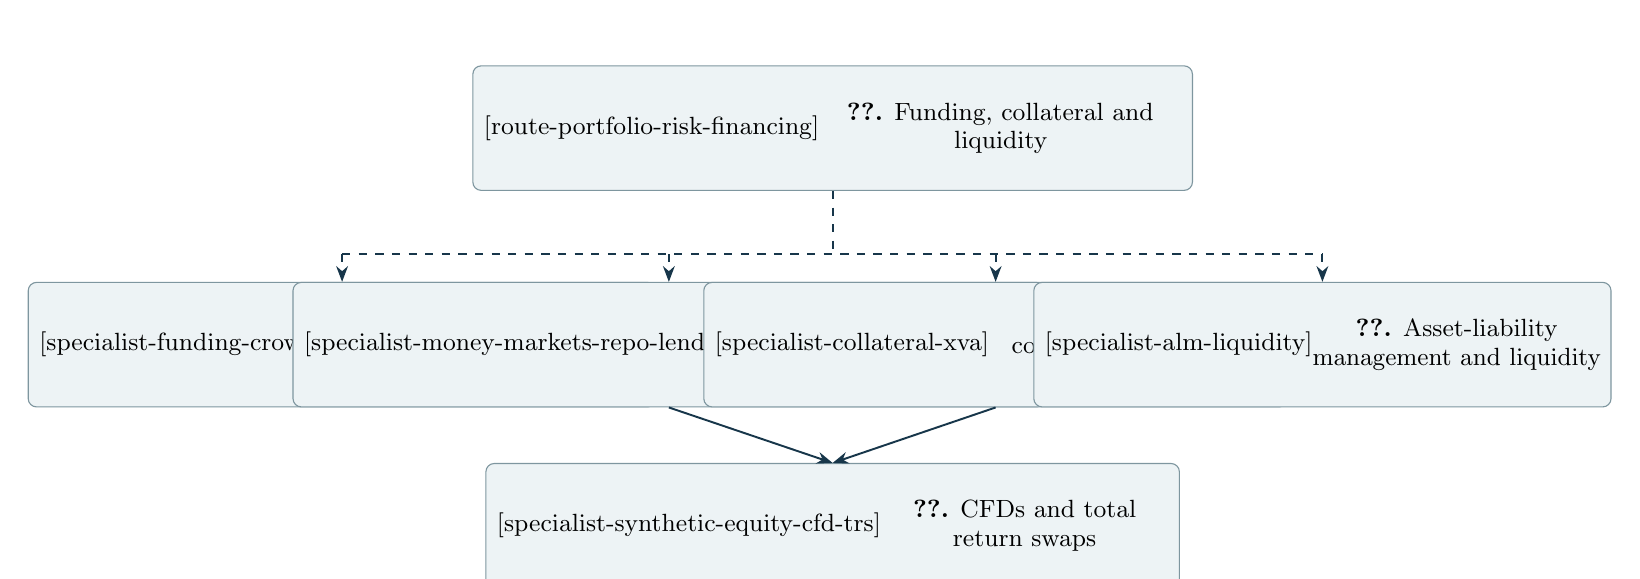
\begin{tikzpicture}[x=1cm,y=1cm]
\node[pathnode] (portfolio-risk-financing) at (6.23,0) {\MeasurePathNode{4.6cm}{\textbf{\ref*{route-portfolio-risk-financing}.} Funding, collateral and liquidity}\hyperref[route-portfolio-risk-financing]{\parbox[c][\pathnodeheight][c]{4.6cm}{\centering \textbf{\ref*{route-portfolio-risk-financing}.} Funding, collateral and liquidity}}};
\node[pathnode] (funding-crowding) at (0.00,-2.75) {\MeasurePathNode{3.65cm}{\textbf{\ref*{specialist-funding-crowding}.} Funding and crowding}\hyperref[specialist-funding-crowding]{\parbox[c][\pathnodeheight][c]{3.65cm}{\centering \textbf{\ref*{specialist-funding-crowding}.} Funding and crowding}}};
\node[pathnode] (money-markets-repo-lending) at (4.15,-2.75) {\MeasurePathNode{3.65cm}{\textbf{\ref*{specialist-money-markets-repo-lending}.} Money markets, repo and securities lending}\hyperref[specialist-money-markets-repo-lending]{\parbox[c][\pathnodeheight][c]{3.65cm}{\centering \textbf{\ref*{specialist-money-markets-repo-lending}.} Money markets, repo and securities lending}}};
\node[pathnode] (collateral-xva) at (8.30,-2.75) {\MeasurePathNode{3.65cm}{\textbf{\ref*{specialist-collateral-xva}.} Collateral, counterparty risk and xVA}\hyperref[specialist-collateral-xva]{\parbox[c][\pathnodeheight][c]{3.65cm}{\centering \textbf{\ref*{specialist-collateral-xva}.} Collateral, counterparty risk and xVA}}};
\node[pathnode] (alm-liquidity) at (12.45,-2.75) {\MeasurePathNode{3.65cm}{\textbf{\ref*{specialist-alm-liquidity}.} Asset-liability management and liquidity}\hyperref[specialist-alm-liquidity]{\parbox[c][\pathnodeheight][c]{3.65cm}{\centering \textbf{\ref*{specialist-alm-liquidity}.} Asset-liability management and liquidity}}};
\node[pathnode] (synthetic-equity-cfd-trs) at (6.23,-5.05) {\MeasurePathNode{3.65cm}{\textbf{\ref*{specialist-synthetic-equity-cfd-trs}.} CFDs and total return swaps}\hyperref[specialist-synthetic-equity-cfd-trs]{\parbox[c][\pathnodeheight][c]{3.65cm}{\centering \textbf{\ref*{specialist-synthetic-equity-cfd-trs}.} CFDs and total return swaps}}};
\draw[entryline] (portfolio-risk-financing.south) -- (6.23,-1.60);
\draw[entryline] (0.00,-1.60) -- (12.45,-1.60);
\draw[entryarrow] (0.00,-1.60) -- (funding-crowding.north);
\draw[entryarrow] (4.15,-1.60) -- (money-markets-repo-lending.north);
\draw[entryarrow] (8.30,-1.60) -- (collateral-xva.north);
\draw[entryarrow] (12.45,-1.60) -- (alm-liquidity.north);
\draw[patharrow] (money-markets-repo-lending.south) -- (synthetic-equity-cfd-trs.north);
\draw[patharrow] (collateral-xva.south) -- (synthetic-equity-cfd-trs.north);
\end{tikzpicture}\end{center}
\hyperref[learning-map]{Return to the whole-guide DAG.}
\Needspace{12\baselineskip}
\subsection{Funding liquidity, crowding and arbitrage capital}\label{specialist-funding-crowding}
\textbf{Specialist pathway.} In \hyperref[route-portfolio-risk-financing]{Funding, collateral and liquidity}.

\textbf{Outcome.} Trace how margin, leverage, funding runs and crowded positions turn small shocks into forced liquidations.

\textbf{Prerequisites.} Funding, collateral and liquidity overview.

\textbf{Review first.} \hyperref[route-portfolio-risk-financing]{Funding, collateral and liquidity}.

\textbf{Required readings, in order}
\begin{enumerate}\raggedright
\Needspace{5\baselineskip}\item \href{institutional_quantitative_finance_reading_list.pdf\#exp-brunnermeier-pedersen-liquidity}{Markus K. Brunnermeier and Lasse Heje Pedersen, Market Liquidity and Funding Liquidity}\CataloguePage{177}\NoteKey{exp-brunnermeier-pedersen-liquidity}\par \textbf{Theory.} Link market and funding liquidity spirals.
\Needspace{5\baselineskip}\item \href{institutional_quantitative_finance_reading_list.pdf\#wide-shleifer-vishny-limits}{Andrei Shleifer and Robert W. Vishny, ``The Limits of Arbitrage''}\CataloguePage{34}\NoteKey{wide-shleifer-vishny-limits}\par \textbf{Theory.} See why arbitrage is weakest when needed.
\Needspace{5\baselineskip}\item \href{institutional_quantitative_finance_reading_list.pdf\#wide-garleanu-pedersen-margin}{Nicolae Gârleanu and Lasse Heje Pedersen, ``Margin-based Asset Pricing and Deviations from the Law of One Price''}\CataloguePage{178}\NoteKey{wide-garleanu-pedersen-margin}\par \textbf{Theory.} Price margin constraints and basis deviations.
\Needspace{5\baselineskip}\item \href{institutional_quantitative_finance_reading_list.pdf\#wide-adrian-shin-leverage}{Tobias Adrian and Hyun Song Shin, ``Liquidity and leverage''}\CataloguePage{178}\NoteKey{wide-adrian-shin-leverage}\par \textbf{Evidence.} Study procyclical dealer leverage.
\Needspace{5\baselineskip}\item \href{institutional_quantitative_finance_reading_list.pdf\#wide-gorton-metrick-repo}{Gary Gorton and Andrew Metrick, ``Securitized banking and the run on repo''}\CataloguePage{177}\NoteKey{wide-gorton-metrick-repo}\par \textbf{Evidence.} Read the 2007--08 run on repo.
\Needspace{5\baselineskip}\item \href{institutional_quantitative_finance_reading_list.pdf\#wide-he-kelly-manela}{Zhiguo He, Bryan Kelly and Asaf Manela, ``Intermediary asset pricing: New evidence from many asset classes''}\CataloguePage{33}\NoteKey{wide-he-kelly-manela}\par \textbf{Evidence.} Price intermediary capital across assets.
\Needspace{5\baselineskip}\item \href{institutional_quantitative_finance_reading_list.pdf\#exp-khandani-lo-quant-meltdown}{Amir E. Khandani and Andrew W. Lo, What Happened to the Quants in August 2007? Evidence from Factors and Transactions Data; published DOI}\CataloguePage{178}\NoteKey{exp-khandani-lo-quant-meltdown}\par \textbf{Evidence.} Study the 2007 quant crowding event.
\Needspace{5\baselineskip}\item \href{institutional_quantitative_finance_reading_list.pdf\#wide-mitchell-pulvino-crashes}{Mark Mitchell and Todd Pulvino, ``Arbitrage crashes and the speed of capital''}\CataloguePage{179}\NoteKey{wide-mitchell-pulvino-crashes}\par \textbf{Evidence.} See prime-broker funding withdrawal in 2008.
\Needspace{5\baselineskip}\item \href{institutional_quantitative_finance_reading_list.pdf\#wide-pedersen-exit}{Lasse Heje Pedersen, ``When Everyone Runs for the Exit''}\CataloguePage{179}\NoteKey{wide-pedersen-exit}\par \textbf{Theory.} Model crowded exits.
\Needspace{5\baselineskip}\item \href{institutional_quantitative_finance_reading_list.pdf\#wide-cs-archegos}{Paul, Weiss, Rifkind, Wharton \& Garrison LLP for the Credit Suisse Special Committee, ``Credit Suisse Group Special Committee of the Board of Directors Report on Archegos Capital Management''}\CataloguePage{179}\NoteKey{wide-cs-archegos}\par \textbf{Evidence.} Study swap financing and risk-control failure.
\Needspace{5\baselineskip}\item \href{institutional_quantitative_finance_reading_list.pdf\#exp-bis-august-2024-carry-unwind}{Matteo Aquilina, Marco Jacopo Lombardi, Andreas Schrimpf, and Vladyslav Sushko, The Market Turbulence and Carry Trade Unwind of August 2024}\CataloguePage{179}\NoteKey{exp-bis-august-2024-carry-unwind}\par \textbf{Evidence.} Analyse a recent carry unwind.
\Needspace{5\baselineskip}\item \href{institutional_quantitative_finance_reading_list.pdf\#w3-siriwardane-segmented-arbitrage}{Emil N. Siriwardane, Adi Sunderam and Jonathan Wallen, ``Segmented Arbitrage''}\CataloguePage{179}\NoteKey{w3-siriwardane-segmented-arbitrage}\par \textbf{Evidence.} See segmented frictions across 32 arbitrage spreads.
\end{enumerate}
\Needspace{5\baselineskip}\textbf{Checkpoint.} Choose one deleveraging episode (2007, 2008, 2020 or 2024); document the funding trigger, margin changes, crowded positions and price impact, and estimate how much an overlap-based crowding measure would have warned in advance.

\textbf{Optional branches.} \href{institutional_quantitative_finance_reading_list.pdf\#wide-copeland-repo-runs}{Compare tri-party repo runs.}\BranchPage{177} \href{institutional_quantitative_finance_reading_list.pdf\#wide-pozsar-shadow}{Map shadow-banking funding chains.}\BranchPage{178} \href{institutional_quantitative_finance_reading_list.pdf\#w3-anderson-du-schlusche-arbitrage}{Trace a funding shock into CIP arbitrage.}\BranchPage{282} \href{institutional_quantitative_finance_reading_list.pdf\#w3-kyle-crowded-markets}{Model trading with misperceived crowding.}\BranchPage{179} \href{institutional_quantitative_finance_reading_list.pdf\#w4-chincarini-crowded-anomalies}{Link anomaly returns to crowding and crash risk.}\BranchPage{194} \href{institutional_quantitative_finance_reading_list.pdf\#w4-vonbeschwitz-passive-shorting}{See passive ownership change securities-lending supply.}\BranchPage{186} \href{institutional_quantitative_finance_reading_list.pdf\#w5-fleckenstein-longstaff-renting}{Estimate balance-sheet rental costs.}\BranchPage{181} \href{institutional_quantitative_finance_reading_list.pdf\#w5-klingler-sundaresan}{Explain negative swap spreads.}\BranchPage{181}
\par{\small \hyperref[learning-map]{Learning pathway DAG} \textbar{} \hyperref[route-portfolio-risk-financing]{Section overview} \textbar{} \hyperref[map-portfolio-risk-financing]{Section DAG}\NoteKey{funding-crowding}}
\Needspace{12\baselineskip}
\subsection{Money markets, repo and securities lending}\label{specialist-money-markets-repo-lending}
\textbf{Specialist pathway.} In \hyperref[route-portfolio-risk-financing]{Funding, collateral and liquidity}.

\textbf{Outcome.} Price short-term cash and collateral financing, distinguish repo from securities lending, and test funding-liquidity exposure with dated benchmark, fund and transaction evidence.

\textbf{Prerequisites.} Funding, collateral and liquidity; discounting, credit exposure, collateral and margin basics.

\textbf{Review first.} \hyperref[route-portfolio-risk-financing]{Funding, collateral and liquidity}.

\textbf{Required readings, in order}
\begin{enumerate}\raggedright
\Needspace{5\baselineskip}\item \href{institutional_quantitative_finance_reading_list.pdf\#gap-money-cp-cd-primer}{Matteo Aquilina, Andreas Schrimpf and Karamfil Todorov, CP and CDs Markets: A Primer}\CataloguePage{234}\NoteKey{gap-money-cp-cd-primer}\par \textbf{Mechanics.} Map CP/CD issuers, investors, tenor and primary placement to alternatives for secured funding.
\Needspace{5\baselineskip}\item \href{institutional_quantitative_finance_reading_list.pdf\#al-icma}{ICMA European Repo and Collateral Council, Repo FAQ 13: ``What is the difference between repo and securities lending?''}\CataloguePage{184}\NoteKey{al-icma}\par \textbf{Mechanics.} Separate repo cash financing, specials and securities borrowing fee/rebate economics.
\Needspace{5\baselineskip}\item \href{institutional_quantitative_finance_reading_list.pdf\#breadth-nyfed-repo-rates}{Federal Reserve Bank of New York, Reference Rates: TGCR, BGCR and SOFR; Additional Information about Reference Rates}\CataloguePage{184}\NoteKey{breadth-nyfed-repo-rates}\par \textbf{Data.} Define TGCR/BGCR/SOFR pools, publication, distribution and revision rules before using a funding proxy.
\Needspace{5\baselineskip}\item \href{institutional_quantitative_finance_reading_list.pdf\#exp-cordes-infante-repo-issuance-qt}{Lucy Cordes and Sebastian Infante, Repo Rate Sensitivity to Treasury Issuance and Quantitative Tightening}\CataloguePage{177}\NoteKey{exp-cordes-infante-repo-issuance-qt}\par \textbf{Evidence.} Link Treasury supply and balance-sheet constraints to observed repo rates rather than inferring a stable spread.
\Needspace{5\baselineskip}\item \href{institutional_quantitative_finance_reading_list.pdf\#al-duffie}{Darrell Duffie, Nicolae G\^arleanu and Lasse Heje Pedersen, ``Securities Lending, Shorting, and Pricing''}\CataloguePage{183}\NoteKey{al-duffie}\par \textbf{Valuation.} Model security-lending search frictions and the economics of locating a particular issue.
\Needspace{5\baselineskip}\item \href{institutional_quantitative_finance_reading_list.pdf\#al-isla}{International Securities Lending Association, \emph{Securities Lending Best Practice Handbook}; downloadable compilation}\CataloguePage{183}\NoteKey{al-isla}\par \textbf{Implementation.} Check loan lifecycle, collateral, margin, recall and operational controls.
\Needspace{5\baselineskip}\item \href{institutional_quantitative_finance_reading_list.pdf\#catalogue-0897}{Taisiya Sikorskaya, ``Institutional Investor Mandates, Securities Lending, and Short-Selling Constraints\textquotesingle\textquotesingle}\CataloguePage{185}\NoteKey{catalogue-0897}\par \textbf{Evidence.} Use the institutional lending study to test mandate heterogeneity and realized revenue.
\Needspace{5\baselineskip}\item \href{institutional_quantitative_finance_reading_list.pdf\#gap-money-nmfp-data}{U.S. Securities and Exchange Commission, Form N-MFP Data Sets; SEC series and class identification file}\CataloguePage{235}\NoteKey{gap-money-nmfp-data}\par \textbf{Data.} Build point-in-time MMF holdings and liquidity exposure from as-filed N-MFP data.
\Needspace{5\baselineskip}\item \href{institutional_quantitative_finance_reading_list.pdf\#gap-money-sec-2023-reform}{U.S. Securities and Exchange Commission, Money Market Fund Reforms; Full final-rule PDF}\CataloguePage{235}\NoteKey{gap-money-sec-2023-reform}\par \textbf{Implementation.} Apply dated US money-fund liquidity and flow rules to a run scenario.
\Needspace{5\baselineskip}\item \href{institutional_quantitative_finance_reading_list.pdf\#gap-money-prime-fund-runs}{Marco Cipriani and Gabriele La Spada, Sophisticated and Unsophisticated Runs}\CataloguePage{234}\NoteKey{gap-money-prime-fund-runs}\par \textbf{Evidence.} Compare a historical prime-fund run with the model and separate empirical episode from current regulation.
\Needspace{5\baselineskip}\item \href{institutional_quantitative_finance_reading_list.pdf\#exp-brunnermeier-pedersen-liquidity}{Markus K. Brunnermeier and Lasse Heje Pedersen, Market Liquidity and Funding Liquidity}\CataloguePage{177}\NoteKey{exp-brunnermeier-pedersen-liquidity}\par \textbf{Valuation.} Connect haircut shocks, margin and funding constraints to a liquidity spiral.
\Needspace{5\baselineskip}\item \href{institutional_quantitative_finance_reading_list.pdf\#latest-copeland-repo-premium-2026}{Adam Copeland and Owen Engbretson, Repo and the Liquidity Risk Premium}\CataloguePage{177}\NoteKey{latest-copeland-repo-premium-2026}\par \textbf{Liquidity pricing.} Trace how dealer liquidity buffers and reserve conditions affect repo premia under the study model.
\Needspace{5\baselineskip}\item \href{institutional_quantitative_finance_reading_list.pdf\#w5-duffie-special-repo}{Darrell Duffie, ``Special Repo Rates''}\CataloguePage{236}\NoteKey{w5-duffie-special-repo}\par \textbf{Mechanics.} Understand specialness in collateral-specific repo.
\end{enumerate}
\Needspace{5\baselineskip}\textbf{Checkpoint.} For a dated Treasury-financing and cash-investment case, map the trade's security, cash lender, collateral, term, haircut, rebate or repo rate, margin and recall terms. Compare the contract economics with the correctly dated TGCR/BGCR/SOFR observation, estimate an MMF liquidity shock from as-filed data, and run a haircut/rollover stress. Flag rates, lending fees and portfolio holdings that are proxies rather than executable quotes. Distinguish the model liquidity-risk premium from a collateral-specific executable repo rate.

\textbf{Optional branches.} \href{institutional_quantitative_finance_reading_list.pdf\#catalogue-0900}{Examine lending recall optionality when the asset is scarce.}\BranchPage{185} \href{institutional_quantitative_finance_reading_list.pdf\#exp-barth-kahn-treasury-basis}{Study repo financing in a Treasury cash-futures basis position.}\BranchPage{180} \href{institutional_quantitative_finance_reading_list.pdf\#wide-choudhry-repo}{Learn repo mechanics and GMRA documentation.}\BranchPage{178} \href{institutional_quantitative_finance_reading_list.pdf\#wide-afonso-lagos}{Model fed funds trade dynamics.}\BranchPage{235} \href{institutional_quantitative_finance_reading_list.pdf\#w4-greppmair-jank-collateral}{Study collateral scarcity and securities-lending facilities.}\BranchPage{186} \href{institutional_quantitative_finance_reading_list.pdf\#w5-krishnamurthy-nagel-orlov}{Size the 2007--08 repo run.}\BranchPage{236} \href{institutional_quantitative_finance_reading_list.pdf\#w5-schmidt-timmermann-wermers}{Study money-fund runs with daily flows.}\BranchPage{236} \href{institutional_quantitative_finance_reading_list.pdf\#w5-covitz-liang-suarez}{Trace the ABCP collapse.}\BranchPage{236}
\par{\small \hyperref[learning-map]{Learning pathway DAG} \textbar{} \hyperref[route-portfolio-risk-financing]{Section overview} \textbar{} \hyperref[map-portfolio-risk-financing]{Section DAG}\NoteKey{money-markets-repo-lending}}
\Needspace{12\baselineskip}
\subsection{Collateral, counterparty risk and xVA}\label{specialist-collateral-xva}
\textbf{Specialist pathway.} In \hyperref[route-portfolio-risk-financing]{Funding, collateral and liquidity}.

\textbf{Outcome.} Build a consistent exposure and valuation-adjustment chain from contract terms to margin and funding.

\textbf{Prerequisites.} Funding, collateral and liquidity; bond cash flows, credit loss, discounting and option exercise.

\textbf{Review first.} \hyperref[route-portfolio-risk-financing]{Funding, collateral and liquidity}.

\textbf{Required readings, in order}
\begin{enumerate}\raggedright
\Needspace{5\baselineskip}\item \href{institutional_quantitative_finance_reading_list.pdf\#gap-gregory5}{Jon Gregory, The xVA Challenge: A Valuation Adjustment Framework for Modern Derivatives Markets}\CataloguePage{182}\NoteKey{gap-gregory5}\par \textbf{Current framework.} Use the fifth-edition map of counterparty, collateral, margin and capital adjustments.
\Needspace{5\baselineskip}\item \href{institutional_quantitative_finance_reading_list.pdf\#exp-piterbarg-collateral-funding}{Vladimir Piterbarg, Funding beyond discounting: collateral agreements and derivatives pricing}\CataloguePage{181}\NoteKey{exp-piterbarg-collateral-funding}\par \textbf{Contractual discounting.} Translate collateral and funding terms into curves before computing residual adjustments.
\Needspace{5\baselineskip}\item \href{institutional_quantitative_finance_reading_list.pdf\#exp-fujii-shimada-takahashi-multicurve}{Masaaki Fujii; Yasufumi Shimada; Akihiko Takahashi, A Market Model of Interest Rates With Dynamic Basis Spreads in the Presence of Collateral and Multiple Currencies}\CataloguePage{181}\NoteKey{exp-fujii-shimada-takahashi-multicurve}\par \textbf{Basis risk.} Keep tenor, currency and collateral-basis exposures consistent.
\Needspace{5\baselineskip}\item \href{institutional_quantitative_finance_reading_list.pdf\#exp-burgard-kjaer-pde-xva}{Christoph Burgard; Mats Kjaer, Partial differential equation representations of derivatives with bilateral counterparty risk and funding costs; publisher addendum; original paper PDF}\CataloguePage{182}\NoteKey{exp-burgard-kjaer-pde-xva}\par \textbf{Analytical valuation.} Read the addendum and benchmark bilateral-default/funding assumptions.
\Needspace{5\baselineskip}\item \href{institutional_quantitative_finance_reading_list.pdf\#s6-simm}{ISDA, \emph{ISDA SIMM Methodology}, version 2.8+2506; version 2.8+2512 release}\CataloguePage{181}\NoteKey{s6-simm}\par \textbf{Initial margin.} Pin the effective methodology and distinguish sensitivity margin from variation margin.
\Needspace{5\baselineskip}\item \href{institutional_quantitative_finance_reading_list.pdf\#exp-andersson-gnoatto-deep-xva}{Kristoffer Andersson; Alessandro Gnoatto, Multi-Layer Deep xVA: Structural Credit Models, Measure Changes and Convergence Analysis}\CataloguePage{182}\NoteKey{exp-andersson-gnoatto-deep-xva}\par \textbf{Computational frontier.} Compare the preliminary layered solver with a simpler exposure benchmark.
\end{enumerate}
\Needspace{5\baselineskip}\textbf{Checkpoint.} Define a hypothetical netting set with collateral currency, thresholds, minimum transfer amount, margin period of risk, eligible collateral and default close-out. Produce clean value, exposure, CVA and funding/margin sensitivities with assumptions explicit. Compare an analytical or simple simulation benchmark with an advanced solver only after aligning conventions. Account for netting and collateral once; do not add overlapping adjustments mechanically. No legal netting opinion, regulatory approval or dealer price is inferred.

\textbf{Optional branches.} \href{institutional_quantitative_finance_reading_list.pdf\#wide-green-xva}{Read a practitioner xVA text.}\BranchPage{182} \href{institutional_quantitative_finance_reading_list.pdf\#wide-duffie-zhu-ccp}{See when central clearing raises exposure.}\BranchPage{182} \href{institutional_quantitative_finance_reading_list.pdf\#wide-andersen-pykhtin-mpor}{Model the margin period of risk in detail.}\BranchPage{183} \href{institutional_quantitative_finance_reading_list.pdf\#w2-menkveld-crowded-ccp}{Measure crowded-position risk at CCPs.}\BranchPage{540} \href{institutional_quantitative_finance_reading_list.pdf\#w2-cpmi-ccp-resilience}{Read CCP resilience guidance.}\BranchPage{540} \href{institutional_quantitative_finance_reading_list.pdf\#w4-piterbarg-ctd-curves}{Approximate cheapest-to-deliver discount curves quickly.}\BranchPage{213} \href{institutional_quantitative_finance_reading_list.pdf\#w5-biais-heider-hoerova}{Design margins against risk-taking.}\BranchPage{540} \href{institutional_quantitative_finance_reading_list.pdf\#w5-duffie-scheicher-vuillemey}{Estimate collateral demand from clearing.}\BranchPage{540} \href{institutional_quantitative_finance_reading_list.pdf\#w5-menkveld-vuillemey}{Review CCP economics.}\BranchPage{540}
\par{\small \hyperref[learning-map]{Learning pathway DAG} \textbar{} \hyperref[route-portfolio-risk-financing]{Section overview} \textbar{} \hyperref[map-portfolio-risk-financing]{Section DAG}\NoteKey{collateral-xva}}
\Needspace{12\baselineskip}
\subsection{Asset-liability management and liquidity}\label{specialist-alm-liquidity}
\textbf{Specialist pathway.} In \hyperref[route-portfolio-risk-financing]{Funding, collateral and liquidity}.

\textbf{Outcome.} Choose a liability hedge that remains fundable through rate shocks, margin calls and asset sales.

\textbf{Prerequisites.} Funding, collateral and liquidity; duration, surplus valuation and collateral management.

\textbf{Review first.} \hyperref[route-portfolio-risk-financing]{Funding, collateral and liquidity}.

\textbf{Required readings, in order}
\begin{enumerate}\raggedright
\Needspace{5\baselineskip}\item \href{institutional_quantitative_finance_reading_list.pdf\#depth-alm-sharpe-tint-1990}{William F. Sharpe and Lawrence G. Tint, Liabilities---A New Approach}\CataloguePage{113}\NoteKey{depth-alm-sharpe-tint-1990}\par \textbf{Valuation.} Frame risk relative to promised payments rather than asset returns alone.
\Needspace{5\baselineskip}\item \href{institutional_quantitative_finance_reading_list.pdf\#depth-alm-hoevenaars-2008}{Roy P. M. M. Hoevenaars, Roderick D. J. Molenaar, Peter C. Schotman and Tom B. M. Steenkamp, Strategic Asset Allocation with Liabilities: Beyond Stocks and Bonds}\CataloguePage{113}\NoteKey{depth-alm-hoevenaars-2008}\par \textbf{Evidence.} Study long-horizon inflation and real-rate covariance with liabilities.
\Needspace{5\baselineskip}\item \href{institutional_quantitative_finance_reading_list.pdf\#depth-alm-ifrs17-discount}{IFRS Foundation, IFRS 17, Insurance Contracts, especially B74--B78}\CataloguePage{114}\NoteKey{depth-alm-ifrs17-discount}\par \textbf{Mechanics.} Specify the relevant liability discounting and accounting basis.
\Needspace{5\baselineskip}\item \href{institutional_quantitative_finance_reading_list.pdf\#depth-alm-eiopa-rfr-2026}{European Insurance and Occupational Pensions Authority, Updated Risk-Free-Rate Technical Documentation and calculation examples}\CataloguePage{114}\NoteKey{depth-alm-eiopa-rfr-2026}\par \textbf{Data.} Inspect the method scheduled for January 2027 as a prospective sensitivity, separate from the October 2026 base regime.
\Needspace{5\baselineskip}\item \href{institutional_quantitative_finance_reading_list.pdf\#depth-alm-tpr-ldi}{The Pensions Regulator, Using Leveraged Liability-Driven Investment}\CataloguePage{113}\NoteKey{depth-alm-tpr-ldi}\par \textbf{Mechanics.} Read current pension LDI operational and liquidity expectations.
\Needspace{5\baselineskip}\item \href{institutional_quantitative_finance_reading_list.pdf\#depth-alm-bis-firesales-2024}{Gabor Pinter, Emil Siriwardane and Danny Walker, Fire Sales of Safe Assets}\CataloguePage{114}\NoteKey{depth-alm-bis-firesales-2024}\par \textbf{Evidence.} Assess how collateral calls can force asset sales.
\Needspace{5\baselineskip}\item \href{institutional_quantitative_finance_reading_list.pdf\#depth-alm-boe-swes-2024}{Bank of England, System-Wide Exploratory Scenario Exercise: Final Report}\CataloguePage{114}\NoteKey{depth-alm-boe-swes-2024}\par \textbf{Evidence.} Use a systemwide exploratory stress as a bounded scenario.
\Needspace{5\baselineskip}\item \href{institutional_quantitative_finance_reading_list.pdf\#exp-brunnermeier-pedersen-liquidity}{Markus K. Brunnermeier and Lasse Heje Pedersen, Market Liquidity and Funding Liquidity}\CataloguePage{177}\NoteKey{exp-brunnermeier-pedersen-liquidity}\par \textbf{Valuation.} Link funding and market liquidity in an unwind.
\Needspace{5\baselineskip}\item \href{institutional_quantitative_finance_reading_list.pdf\#s6-simm}{ISDA, \emph{ISDA SIMM Methodology}, version 2.8+2506; version 2.8+2512 release}\CataloguePage{181}\NoteKey{s6-simm}\par \textbf{Implementation.} Account for initial-margin requirements on derivatives hedges.
\Needspace{5\baselineskip}\item \href{institutional_quantitative_finance_reading_list.pdf\#gap-rates-treasury-futures-delivery}{CME Group, The Treasury Futures Delivery Process, Eighth Edition; CME conversion-factor detail}\CataloguePage{224}\NoteKey{gap-rates-treasury-futures-delivery}\par \textbf{Implementation.} Include futures delivery and basis risk in duration overlays.
\Needspace{5\baselineskip}\item \href{institutional_quantitative_finance_reading_list.pdf\#w3-jansen-pension-liquidity}{Kristy A. E. Jansen, Sven Klingler, Angelo Ranaldo and Patty Duijm, ``Pension Liquidity Risk''}\CataloguePage{115}\NoteKey{w3-jansen-pension-liquidity}\par \textbf{Evidence.} Measure swap margin-call risk in pension hedging.
\end{enumerate}
\Needspace{5\baselineskip}\textbf{Checkpoint.} Select one pension or insurer regime and its operative dated discounting basis. Project five years of liabilities and asset income under base, inflation and real-rate shocks; calculate surplus duration and hedge cost. Add daily margin, haircuts, forced sales and liquidity buffers. Treat the January 2027 EIOPA method only as a prospective sensitivity, not the October 2026 base. Label synthetic cash-flow and collateral inputs.

\textbf{Optional branches.} \href{institutional_quantitative_finance_reading_list.pdf\#wide-goldstein-jiang-ng}{Study fund fragility from illiquid assets.}\BranchPage{115} \href{institutional_quantitative_finance_reading_list.pdf\#wide-swensen-pioneering}{Read the endowment model.}\BranchPage{115} \href{institutional_quantitative_finance_reading_list.pdf\#w3-li-life-insurers-spreads}{Link insurer duration gaps to credit spreads.}\BranchPage{115} \href{institutional_quantitative_finance_reading_list.pdf\#w3-ma-xiao-zeng-swing}{Compare bank and fund liquidity provision.}\BranchPage{115}
\par{\small \hyperref[learning-map]{Learning pathway DAG} \textbar{} \hyperref[route-portfolio-risk-financing]{Section overview} \textbar{} \hyperref[map-portfolio-risk-financing]{Section DAG}\NoteKey{alm-liquidity}}
\Needspace{12\baselineskip}
\subsection{CFDs, total return swaps and synthetic equity financing}\label{specialist-synthetic-equity-cfd-trs}
\textbf{Specialist pathway.} In \hyperref[route-portfolio-risk-financing]{Funding, collateral and liquidity}.

\textbf{Outcome.} Price a CFD or equity total return swap from its financing, dividend, borrow and margin terms; compare it with futures, listed total return futures and cash financing; and identify the counterparty, disclosure and tax exposures it creates.

\textbf{Prerequisites.} Funding, collateral and liquidity overview; repo and securities lending; collateral, margin and xVA.

\textbf{Review first.} \hyperref[route-portfolio-risk-financing]{Funding, collateral and liquidity}; \hyperref[specialist-money-markets-repo-lending]{Money markets, repo and securities lending}; \hyperref[specialist-collateral-xva]{Collateral, counterparty risk and xVA}.

\textbf{Required readings, in order}
\begin{enumerate}\raggedright
\Needspace{5\baselineskip}\item \href{institutional_quantitative_finance_reading_list.pdf\#s7-hulloptions}{John C. Hull, \emph{Options, Futures, and Other Derivatives}, 11th Global ed. (published 2021; copyright 2022)}\CataloguePage{117}\NoteKey{s7-hulloptions}\par\emph{Selection:} Swap chapters covering equity and total return swaps (topic selection; chapter numbering is not inferred).\par \textbf{Mechanics.} Set out the cash flows of equity and total return swaps.
\Needspace{5\baselineskip}\item \href{institutional_quantitative_finance_reading_list.pdf\#cfd-brown-dark-davis-2010}{Christine Brown, Jonathan Dark and Kevin Davis, ``Exchange traded contracts for difference: Design, pricing, and effects''}\CataloguePage{186}\NoteKey{cfd-brown-dark-davis-2010}\par \textbf{Mechanics.} Compare CFD contract designs and test their pricing.
\Needspace{5\baselineskip}\item \href{institutional_quantitative_finance_reading_list.pdf\#cfd-foster-lee-liu-2019}{F. Douglas Foster, Adrian D. Lee and Wai-Man Liu, ``CFDs, forwards, futures and the cost-of-carry''}\CataloguePage{187}\NoteKey{cfd-foster-lee-liu-2019}\par \textbf{Valuation.} Price a CFD by cost of carry against forwards and futures.
\Needspace{5\baselineskip}\item \href{institutional_quantitative_finance_reading_list.pdf\#al-duffie}{Darrell Duffie, Nicolae G\^arleanu and Lasse Heje Pedersen, ``Securities Lending, Shorting, and Pricing''}\CataloguePage{183}\NoteKey{al-duffie}\par \textbf{Theory.} Model the borrow fee that a short CFD or swap passes through.
\Needspace{5\baselineskip}\item \href{institutional_quantitative_finance_reading_list.pdf\#cfd-binsbergen-rf-2022}{Jules H. van Binsbergen, William F. Diamond and Marco Grotteria, ``Risk-free interest rates''}\CataloguePage{187}\NoteKey{cfd-binsbergen-rf-2022}\par \textbf{Data.} Take a financing benchmark from option-implied risk-free rates.
\Needspace{5\baselineskip}\item \href{institutional_quantitative_finance_reading_list.pdf\#cfd-hazelkorn-2023}{Todd M. Hazelkorn, Tobias J. Moskowitz and Kaushik Vasudevan, ``Beyond Basis Basics: Liquidity Demand and Deviations from the Law of One Price''}\CataloguePage{187}\NoteKey{cfd-hazelkorn-2023}\par \textbf{Evidence.} Read the implied financing spread in index futures as demand for leverage.
\Needspace{5\baselineskip}\item \href{institutional_quantitative_finance_reading_list.pdf\#cfd-eurex-trf}{Eurex, Index Total Return Futures: a listed solution for implied equity repo trading}\CataloguePage{187}\NoteKey{cfd-eurex-trf}\par \textbf{Implementation.} Compare a bilateral equity swap with a listed total return future.
\Needspace{5\baselineskip}\item \href{institutional_quantitative_finance_reading_list.pdf\#wide-bcbs-iosco-margin}{Basel Committee on Banking Supervision and International Organization of Securities Commissions, ``Margin requirements for non-centrally cleared derivatives''}\CataloguePage{182}\NoteKey{wide-bcbs-iosco-margin}\par \textbf{Regulation.} Apply initial and variation margin rules to uncleared equity swaps.
\Needspace{5\baselineskip}\item \href{institutional_quantitative_finance_reading_list.pdf\#wide-cs-archegos}{Paul, Weiss, Rifkind, Wharton \& Garrison LLP for the Credit Suisse Special Committee, ``Credit Suisse Group Special Committee of the Board of Directors Report on Archegos Capital Management''}\CataloguePage{179}\NoteKey{wide-cs-archegos}\par \textbf{Evidence.} Trace how swap financing, margin settings and concentration failed at one prime broker.
\Needspace{5\baselineskip}\item \href{institutional_quantitative_finance_reading_list.pdf\#cfd-esma-archegos-2022}{Antoine Bouveret and Martin Haferkorn, European Securities and Markets Authority, Leverage and derivatives -- the case of Archegos}\CataloguePage{187}\NoteKey{cfd-esma-archegos-2022}\par \textbf{Data.} Track concentrated swap exposure across dealers with trade-repository data.
\Needspace{5\baselineskip}\item \href{institutional_quantitative_finance_reading_list.pdf\#cfd-aragon-strahan-2012}{George O. Aragon and Philip E. Strahan, ``Hedge funds as liquidity providers: Evidence from the Lehman bankruptcy''}\CataloguePage{187}\NoteKey{cfd-aragon-strahan-2012}\par \textbf{Evidence.} See how a prime broker's failure reaches its clients' positions.
\Needspace{5\baselineskip}\item \href{institutional_quantitative_finance_reading_list.pdf\#cfd-hu-black-2007}{Henry T. C. Hu and Bernard Black, ``Hedge funds, insiders, and the decoupling of economic and voting ownership: Empty voting and hidden (morphable) ownership''}\CataloguePage{187}\NoteKey{cfd-hu-black-2007}\par \textbf{Evidence.} Recognise empty voting and hidden ownership through equity swaps.
\Needspace{5\baselineskip}\item \href{institutional_quantitative_finance_reading_list.pdf\#cfd-sec-13d-2023}{U.S. Securities and Exchange Commission, Modernization of Beneficial Ownership Reporting: Final Rule}\CataloguePage{188}\NoteKey{cfd-sec-13d-2023}\par \textbf{Regulation.} Apply the 2023 Schedule 13D guidance on cash-settled derivatives.
\Needspace{5\baselineskip}\item \href{institutional_quantitative_finance_reading_list.pdf\#cfd-irs-871m-2026}{Internal Revenue Service, Notice 2026-61: Extension of the Phase-in Period for the Enforcement and Administration of Section 871(m)}\CataloguePage{188}\NoteKey{cfd-irs-871m-2026}\par \textbf{Regulation.} Treat U.S. dividend-equivalent withholding on delta-one swaps and CFDs.
\Needspace{5\baselineskip}\item \href{institutional_quantitative_finance_reading_list.pdf\#cfd-buettner-cumex-2020}{Thiess Buettner, Carolin Holzmann, Felix Kreidl and Hendrik Scholz, ``Withholding-tax non-compliance: the case of cum-ex stock-market transactions''}\CataloguePage{188}\NoteKey{cfd-buettner-cumex-2020}\par \textbf{Evidence.} Study how trades around dividend dates exploited withholding-tax refunds.
\end{enumerate}
\Needspace{5\baselineskip}\textbf{Checkpoint.} Build the cash flows of a one-year long CFD and an equity total return swap on the same index: daily financing at a benchmark plus spread, dividend pass-through net of withholding, the borrow fee on the short side and variation margin. Compare the all-in financing rate with the implied financing in index futures and a listed total return future. Stress a 30 percent gap move on a concentrated position split across three dealers, and state what each dealer, a regulator and the issuer could see under current disclosure and reporting rules.

\textbf{Optional branches.} \href{institutional_quantitative_finance_reading_list.pdf\#w5-fleckenstein-longstaff-renting}{Price the balance-sheet rental cost behind dealer financing.}\BranchPage{181} \href{institutional_quantitative_finance_reading_list.pdf\#cfd-sec-10b1-withdrawal-2025}{Note the withdrawn U.S. proposal for large swap-position reporting.}\BranchPage{188} \href{institutional_quantitative_finance_reading_list.pdf\#s6-simm}{Compute initial margin for an equity swap book.}\BranchPage{181} \href{institutional_quantitative_finance_reading_list.pdf\#roadmap-perpetual-fundamentals}{Compare perpetual futures, which share the CFD funding mechanism.}\BranchPage{446} \href{institutional_quantitative_finance_reading_list.pdf\#wide-brav-activism}{Connect hidden ownership to activist campaigns.}\BranchPage{197}
\par{\small \hyperref[learning-map]{Learning pathway DAG} \textbar{} \hyperref[route-portfolio-risk-financing]{Section overview} \textbar{} \hyperref[map-portfolio-risk-financing]{Section DAG}\NoteKey{synthetic-equity-cfd-trs}}
\clearpage
\section{Market microstructure and market making}\label{route-execution-market-making}
\label{route-6}
\textbf{Learning sequence.} Study order-book mechanics and market making, then order-book learning, options market making, dealer market making in bonds and swaps, and simulation; FX dealing builds on bond and swap dealing, and high-frequency trading is a separate entry point. Crypto venues apply the same tools in Part VI.

\textbf{Section goals.} Across its pathways, this section teaches you to:
\begin{itemize}[leftmargin=1.4em,itemsep=0pt,topsep=1pt]
\item derive inventory-aware quotes and model queues and fill probabilities (\hyperref[specialist-market-making-lob]{\ref*{specialist-market-making-lob}})
\item train order-book prediction models with leakage-free evaluation (\hyperref[specialist-lob-deep-learning]{\ref*{specialist-lob-deep-learning}})
\item explain option spreads and the routing and cost of retail option orders (\hyperref[specialist-options-execution]{\ref*{specialist-options-execution}})
\item quote bonds and swaps on request within dealer balance-sheet limits (\hyperref[specialist-bond-swap-dealer-market-making]{\ref*{specialist-bond-swap-dealer-market-making}})
\item build and validate market simulators (\hyperref[specialist-market-simulation]{\ref*{specialist-market-simulation}})
\item price an FX client franchise, choose between internalising and hedging, and judge last look (\hyperref[specialist-fx-dealer-market-making]{\ref*{specialist-fx-dealer-market-making}})
\item evaluate high-frequency trading, latency races and market design (\hyperref[specialist-hft-market-design]{\ref*{specialist-hft-market-design}})
\end{itemize}
\textbf{Overview outcome.} Evaluate a quoting policy on an order-book replay by fill probability, adverse selection and inventory risk, and state how the result depends on queue-position and self-impact assumptions.

\textbf{Prerequisites.} Common toolkit; limit orders, order-book events and elementary stochastic processes.

\textbf{Review first.} \hyperref[route-common-toolkit]{Common toolkit}.

\textbf{Required readings, in order}
\begin{enumerate}\raggedright
\Needspace{5\baselineskip}\item \href{institutional_quantitative_finance_reading_list.pdf\#alpha-harris}{Larry Harris, \emph{Trading and Exchanges}}\CataloguePage{146}\NoteKey{alpha-harris}\par Start from order types, trading motives and who bears the cost of immediacy.
\Needspace{5\baselineskip}\item \href{institutional_quantitative_finance_reading_list.pdf\#s6-hasbrouck}{Joel Hasbrouck, \emph{Empirical Market Microstructure}}\CataloguePage{146}\NoteKey{s6-hasbrouck}\par Turn trades and quotes into empirical measures of liquidity and price discovery.
\Needspace{5\baselineskip}\item \href{institutional_quantitative_finance_reading_list.pdf\#s6-stoikov}{Marco Avellaneda and Sasha Stoikov, ``High-Frequency Trading in a Limit Order Book''}\CataloguePage{149}\NoteKey{s6-stoikov}\par Use inventory-sensitive quotes and stylised fill intensities as a market-making benchmark, then test their assumptions.
\Needspace{5\baselineskip}\item \href{institutional_quantitative_finance_reading_list.pdf\#exp-cont-kukanov-order-placement}{Rama Cont; Arseniy Kukanov, Optimal order placement in limit order markets; Oxford author manuscript}\CataloguePage{161}\NoteKey{exp-cont-kukanov-order-placement}\par Model placement across venues with uncertain fills and explicit order costs.
\Needspace{5\baselineskip}\item \href{institutional_quantitative_finance_reading_list.pdf\#exp-huang-lehalle-rosenbaum-queue-reactive}{Weibing Huang; Charles-Albert Lehalle; Mathieu Rosenbaum, Simulating and Analyzing Order Book Data: The Queue-Reactive Model}\CataloguePage{161}\NoteKey{exp-huang-lehalle-rosenbaum-queue-reactive}\par Make queue state and event arrival part of the simulation rather than assuming every touched quote fills.
\Needspace{5\baselineskip}\item \href{institutional_quantitative_finance_reading_list.pdf\#exp-noble-rosenbaum-souilmi-reality-gap}{Patrick Noble; Mathieu Rosenbaum; Saad Souilmi, Bridging the Reality Gap in Limit Order Book Simulation}\CataloguePage{166}\NoteKey{exp-noble-rosenbaum-souilmi-reality-gap}\par Test whether a simulator reproduces relevant market responses before using it to rank policies.
\end{enumerate}
\Needspace{5\baselineskip}\textbf{Checkpoint.} Replay one order-book day with order acknowledgements, cancellations, fills and missed fills. Compare a passive limit order with an inventory-limited quote policy using fill probability, adverse selection and inventory risk, and test how the result depends on queue-position and self-impact assumptions.

\textbf{Optional branches.} \href{institutional_quantitative_finance_reading_list.pdf\#section.8.5}{Extend replay into counterfactual and generative market simulation.}\BranchPage{166}
\par\textbf{Continue in this section.} \hyperref[specialist-market-making-lob]{Market making, queues and limit-order-book models}; \hyperref[specialist-lob-deep-learning]{Deep learning on limit-order-book data}; \hyperref[specialist-options-execution]{Options market making and execution costs}; \hyperref[specialist-bond-swap-dealer-market-making]{Bond and swap dealing: RFQs, inventory and balance-sheet capacity}; \hyperref[specialist-market-simulation]{Market simulation and counterfactual testing}; \hyperref[specialist-fx-dealer-market-making]{FX dealing: internalisation, last look and hedging}; \hyperref[specialist-hft-market-design]{High-frequency trading, speed and adverse selection}.
\par{\small \hyperref[learning-map]{Learning pathway DAG} \textbar{} \hyperref[map-execution-market-making]{Section DAG}\NoteKey{execution-market-making}}
\clearpage
\subsection*{Market microstructure and market making: pathway DAG}\phantomsection\label{map-execution-market-making}
\addcontentsline{toc}{subsection}{Market microstructure and market making: pathway DAG}
Start with the section overview's readings, for orientation. Solid arrows show prerequisites within this section. Dashed connectors identify entry points with no further prerequisite in this section; the linked foundations below still apply. Follow the arrows for dependencies and the subsection numbers for reading order. Every node is clickable.
\begin{center}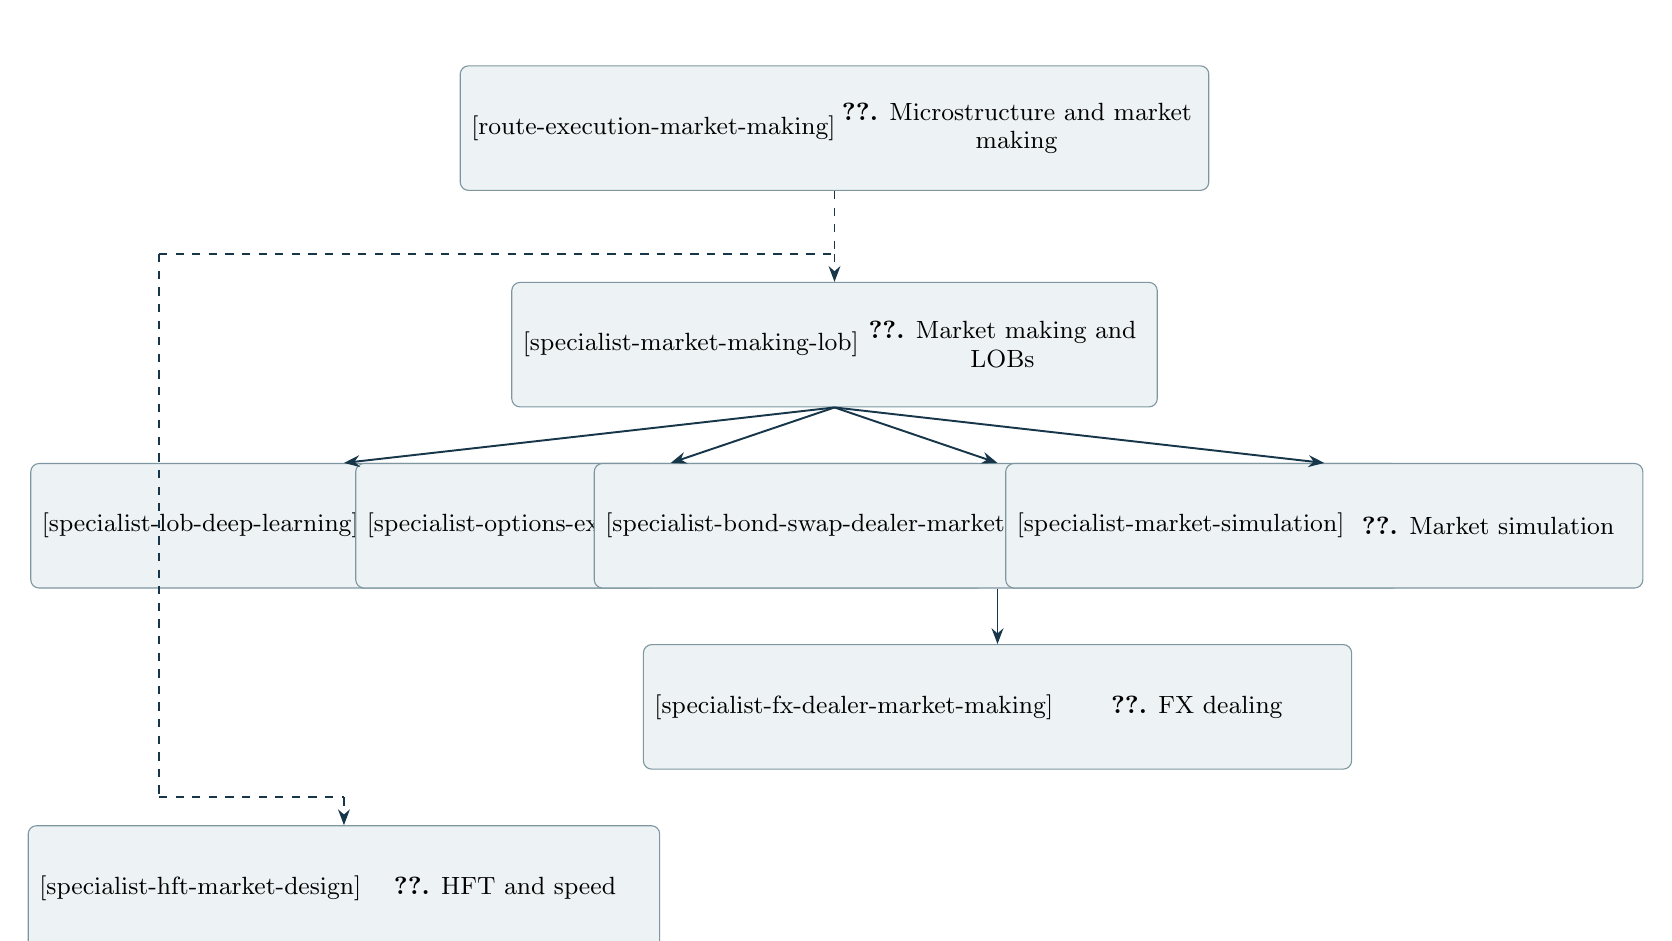
\begin{tikzpicture}[x=1cm,y=1cm]
\node[pathnode] (execution-market-making) at (6.23,0) {\MeasurePathNode{4.6cm}{\textbf{\ref*{route-execution-market-making}.} Microstructure and market making}\hyperref[route-execution-market-making]{\parbox[c][\pathnodeheight][c]{4.6cm}{\centering \textbf{\ref*{route-execution-market-making}.} Microstructure and market making}}};
\node[pathnode] (market-making-lob) at (6.23,-2.75) {\MeasurePathNode{3.65cm}{\textbf{\ref*{specialist-market-making-lob}.} Market making and LOBs}\hyperref[specialist-market-making-lob]{\parbox[c][\pathnodeheight][c]{3.65cm}{\centering \textbf{\ref*{specialist-market-making-lob}.} Market making and LOBs}}};
\node[pathnode] (lob-deep-learning) at (0.00,-5.05) {\MeasurePathNode{3.65cm}{\textbf{\ref*{specialist-lob-deep-learning}.} LOB deep learning}\hyperref[specialist-lob-deep-learning]{\parbox[c][\pathnodeheight][c]{3.65cm}{\centering \textbf{\ref*{specialist-lob-deep-learning}.} LOB deep learning}}};
\node[pathnode] (options-execution) at (4.15,-5.05) {\MeasurePathNode{3.65cm}{\textbf{\ref*{specialist-options-execution}.} Options market making}\hyperref[specialist-options-execution]{\parbox[c][\pathnodeheight][c]{3.65cm}{\centering \textbf{\ref*{specialist-options-execution}.} Options market making}}};
\node[pathnode] (bond-swap-dealer-market-making) at (8.30,-5.05) {\MeasurePathNode{3.65cm}{\textbf{\ref*{specialist-bond-swap-dealer-market-making}.} Bond and swap dealing}\hyperref[specialist-bond-swap-dealer-market-making]{\parbox[c][\pathnodeheight][c]{3.65cm}{\centering \textbf{\ref*{specialist-bond-swap-dealer-market-making}.} Bond and swap dealing}}};
\node[pathnode] (market-simulation) at (12.45,-5.05) {\MeasurePathNode{3.65cm}{\textbf{\ref*{specialist-market-simulation}.} Market simulation}\hyperref[specialist-market-simulation]{\parbox[c][\pathnodeheight][c]{3.65cm}{\centering \textbf{\ref*{specialist-market-simulation}.} Market simulation}}};
\node[pathnode] (fx-dealer-market-making) at (8.30,-7.35) {\MeasurePathNode{3.65cm}{\textbf{\ref*{specialist-fx-dealer-market-making}.} FX dealing}\hyperref[specialist-fx-dealer-market-making]{\parbox[c][\pathnodeheight][c]{3.65cm}{\centering \textbf{\ref*{specialist-fx-dealer-market-making}.} FX dealing}}};
\node[pathnode] (hft-market-design) at (0.00,-9.65) {\MeasurePathNode{3.65cm}{\textbf{\ref*{specialist-hft-market-design}.} HFT and speed}\hyperref[specialist-hft-market-design]{\parbox[c][\pathnodeheight][c]{3.65cm}{\centering \textbf{\ref*{specialist-hft-market-design}.} HFT and speed}}};
\draw[entryline] (execution-market-making.south) -- (6.23,-1.60);
\draw[entryline] (-2.35,-1.60) -- (-2.35,-8.50);
\draw[entryline] (-2.35,-1.60) -- (6.23,-1.60);
\draw[entryarrow] (6.23,-1.60) -- (market-making-lob.north);
\draw[entryline] (-2.35,-8.50) -- (0.00,-8.50);
\draw[entryarrow] (0.00,-8.50) -- (hft-market-design.north);
\draw[patharrow] (market-making-lob.south) -- (lob-deep-learning.north);
\draw[patharrow] (market-making-lob.south) -- (options-execution.north);
\draw[patharrow] (market-making-lob.south) -- (bond-swap-dealer-market-making.north);
\draw[patharrow] (market-making-lob.south) -- (market-simulation.north);
\draw[patharrow] (bond-swap-dealer-market-making.south) -- (fx-dealer-market-making.north);
\end{tikzpicture}\end{center}
\textbf{Bring these foundations with you.}\begin{itemize}
\item \hyperref[specialist-stochastic-calculus-control]{Stochastic calculus and continuous-time control} --- needed by \hyperref[specialist-market-making-lob]{Market making and LOBs}.
\item \hyperref[specialist-statistical-learning-foundations]{Statistical learning foundations and time-series validation} --- needed by \hyperref[specialist-lob-deep-learning]{LOB deep learning}.
\item \hyperref[specialist-option-premia-dealers]{Option returns, variance premia and dealer hedging} --- needed by \hyperref[specialist-options-execution]{Options market making}.
\item \hyperref[route-corporate-credit-capital]{Corporate credit, hybrids and labelled bonds} --- needed by \hyperref[specialist-bond-swap-dealer-market-making]{Bond and swap dealing}.
\item \hyperref[specialist-fx-funding-settlement]{FX forwards, options, fixes and settlement} --- needed by \hyperref[specialist-fx-dealer-market-making]{FX dealing}.
\end{itemize}\hyperref[learning-map]{Return to the whole-guide DAG.}
\Needspace{12\baselineskip}
\subsection{Market making, queues and limit-order-book models}\label{specialist-market-making-lob}
\textbf{Specialist pathway.} In \hyperref[route-execution-market-making]{Market microstructure and market making}.

\textbf{Outcome.} Derive inventory-aware quotes, model queue dynamics and fill probabilities, and evaluate learned order-book signals.

\textbf{Prerequisites.} Market microstructure and market making; stochastic calculus and control.

\textbf{Review first.} \hyperref[route-execution-market-making]{Market microstructure and market making}; \hyperref[specialist-stochastic-calculus-control]{Stochastic calculus and continuous-time control}.

\textbf{Required readings, in order}
\begin{enumerate}\raggedright
\Needspace{5\baselineskip}\item \href{institutional_quantitative_finance_reading_list.pdf\#s6-glosten}{Lawrence R. Glosten and Paul R. Milgrom, ``Bid, Ask and Transaction Prices in a Specialist Market with Heterogeneously Informed Traders''}\CataloguePage{146}\NoteKey{s6-glosten}\par \textbf{Theory.} Start from adverse selection and the spread.
\Needspace{5\baselineskip}\item \href{institutional_quantitative_finance_reading_list.pdf\#catalogue-0527}{Ho and Stoll dealer inventory models}\CataloguePage{147}\NoteKey{catalogue-0527}\par \textbf{Theory.} Add dealer inventory.
\Needspace{5\baselineskip}\item \href{institutional_quantitative_finance_reading_list.pdf\#s6-stoikov}{Marco Avellaneda and Sasha Stoikov, ``High-Frequency Trading in a Limit Order Book''}\CataloguePage{149}\NoteKey{s6-stoikov}\par \textbf{Methods.} Derive inventory-aware quotes.
\Needspace{5\baselineskip}\item \href{institutional_quantitative_finance_reading_list.pdf\#wide-gueant-lehalle-tapia}{Olivier Guéant, Charles-Albert Lehalle and Joaquin Fernandez-Tapia, ``Dealing with the inventory risk: a solution to the market making problem''}\CataloguePage{163}\NoteKey{wide-gueant-lehalle-tapia}\par \textbf{Methods.} Solve the bounded-inventory problem.
\Needspace{5\baselineskip}\item \href{institutional_quantitative_finance_reading_list.pdf\#wide-cartea-jaimungal-ricci}{Álvaro Cartea, Sebastian Jaimungal and Jason Ricci, ``Buy Low, Sell High: A High Frequency Trading Perspective''}\CataloguePage{163}\NoteKey{wide-cartea-jaimungal-ricci}\par \textbf{Methods.} Add short-term alpha and adverse selection.
\Needspace{5\baselineskip}\item \href{institutional_quantitative_finance_reading_list.pdf\#wide-cont-stoikov-talreja}{Rama Cont, Sasha Stoikov and Rishi Talreja, ``A Stochastic Model for Order Book Dynamics''}\CataloguePage{161}\NoteKey{wide-cont-stoikov-talreja}\par \textbf{Methods.} Model the order book as queues.
\Needspace{5\baselineskip}\item \href{institutional_quantitative_finance_reading_list.pdf\#exp-huang-lehalle-rosenbaum-queue-reactive}{Weibing Huang; Charles-Albert Lehalle; Mathieu Rosenbaum, Simulating and Analyzing Order Book Data: The Queue-Reactive Model}\CataloguePage{161}\NoteKey{exp-huang-lehalle-rosenbaum-queue-reactive}\par \textbf{Methods.} Simulate a queue-reactive book.
\Needspace{5\baselineskip}\item \href{institutional_quantitative_finance_reading_list.pdf\#wide-moallemi-yuan-queue}{Ciamac C. Moallemi and Kai Yuan, ``A Model for Queue Position Valuation in a Limit Order Book''}\CataloguePage{161}\NoteKey{wide-moallemi-yuan-queue}\par \textbf{Valuation.} Value queue position.
\Needspace{5\baselineskip}\item \href{institutional_quantitative_finance_reading_list.pdf\#wide-lehalle-mounjid}{Charles-Albert Lehalle and Othmane Mounjid, ``Limit order strategic placement with adverse selection risk and the role of latency''}\CataloguePage{161}\NoteKey{wide-lehalle-mounjid}\par \textbf{Implementation.} Place orders with imbalance and latency.
\Needspace{5\baselineskip}\item \href{institutional_quantitative_finance_reading_list.pdf\#wide-bacry-hawkes}{Emmanuel Bacry, Iacopo Mastromatteo and Jean-François Muzy, ``Hawkes Processes in Finance''}\CataloguePage{162}\NoteKey{wide-bacry-hawkes}\par \textbf{Methods.} Use Hawkes processes for order flow.
\Needspace{5\baselineskip}\item \href{institutional_quantitative_finance_reading_list.pdf\#wide-arroyo-fill-probability}{Álvaro Arroyo, Álvaro Cartea, Fernando Moreno-Pino and Stefan Zohren, ``Deep attentive survival analysis in limit order books: estimating fill probabilities with convolutional-transformers''}\CataloguePage{162}\NoteKey{wide-arroyo-fill-probability}\par \textbf{Methods.} Estimate fill probabilities with survival models.
\Needspace{5\baselineskip}\item \href{institutional_quantitative_finance_reading_list.pdf\#wide-sirignano-cont-universal}{Justin Sirignano and Rama Cont, ``Universal features of price formation in financial markets: perspectives from deep learning''}\CataloguePage{165}\NoteKey{wide-sirignano-cont-universal}\par \textbf{Evidence.} Test universal price-formation features.
\Needspace{5\baselineskip}\item \href{institutional_quantitative_finance_reading_list.pdf\#wide-kolm-deep-ofi}{Petter N. Kolm, Jeremy Turiel and Nicholas Westray, ``Deep order flow imbalance: Extracting alpha at multiple horizons from the limit order book''}\CataloguePage{165}\NoteKey{wide-kolm-deep-ofi}\par \textbf{Methods.} Forecast from order-flow imbalance.
\Needspace{5\baselineskip}\item \href{institutional_quantitative_finance_reading_list.pdf\#wide-gasperov-mm-review}{Bruno Gašperov, Stjepan Begušić, Petra Posedel Šimović and Zvonko Kostanjčar, ``Reinforcement Learning Approaches to Optimal Market Making''}\CataloguePage{164}\NoteKey{wide-gasperov-mm-review}\par \textbf{Validation.} Review RL market-making evaluation weaknesses.
\end{enumerate}
\Needspace{5\baselineskip}\textbf{Checkpoint.} Implement an Avellaneda--Stoikov/Guéant market maker on replayed LOBSTER data with a queue-position fill model; compare P\&L, inventory and adverse selection with and without an order-flow-imbalance signal, and report sensitivity to latency and fill assumptions.

\textbf{Optional branches.} \href{institutional_quantitative_finance_reading_list.pdf\#wide-abergel-lob-book}{Read a monograph on limit-order-book models.}\BranchPage{162} \href{institutional_quantitative_finance_reading_list.pdf\#wide-spooner-mm-rl}{Compare an RL market maker.}\BranchPage{163} \href{institutional_quantitative_finance_reading_list.pdf\#w3-garriott-queuing}{Relate queue position to adverse selection and inventory.}\BranchPage{162} \href{institutional_quantitative_finance_reading_list.pdf\#w3-nutz-webster-warehouse}{Decide when to warehouse or route order flow.}\BranchPage{164} \href{institutional_quantitative_finance_reading_list.pdf\#w3-cartea-toxic-flow}{Detect toxic flow before quoting.}\BranchPage{164} \href{institutional_quantitative_finance_reading_list.pdf\#w4-pulido-rosenbaum-imbalance}{Explain why order-book imbalance predicts prices.}\BranchPage{151} \href{institutional_quantitative_finance_reading_list.pdf\#w4-cartea-broker-informed}{Internalise or externalise toxic informed flow.}\BranchPage{164} \href{institutional_quantitative_finance_reading_list.pdf\#w4-boyce-herdegen-mm-competition}{Make markets against rule-of-thumb competitors.}\BranchPage{164} \href{institutional_quantitative_finance_reading_list.pdf\#w4-gupta-tacit-coordination}{Diagnose tacit coordination among learning market makers.}\BranchPage{164} \href{institutional_quantitative_finance_reading_list.pdf\#w4-cont-degond-xuan-lob}{Model LOB dynamics as order flow plus clearing.}\BranchPage{162} \href{institutional_quantitative_finance_reading_list.pdf\#ex-hendershott-menkveld-2014}{Measure the price pressure that intermediary inventory creates and how fast it decays.}\BranchPage{164}
\par{\small \hyperref[learning-map]{Learning pathway DAG} \textbar{} \hyperref[route-execution-market-making]{Section overview} \textbar{} \hyperref[map-execution-market-making]{Section DAG}\NoteKey{market-making-lob}}
\Needspace{12\baselineskip}
\subsection{Deep learning on limit-order-book data}\label{specialist-lob-deep-learning}
\textbf{Specialist pathway.} In \hyperref[route-execution-market-making]{Market microstructure and market making}.

\textbf{Outcome.} Train and evaluate an order-book prediction model with leakage-free splits, realistic benchmarks and transaction-level usefulness.

\textbf{Prerequisites.} Market making, queues and limit-order-book models (18.1); Statistical learning foundations and time-series validation (4.1).

\textbf{Review first.} \hyperref[specialist-market-making-lob]{Market making, queues and limit-order-book models}; \hyperref[specialist-statistical-learning-foundations]{Statistical learning foundations and time-series validation}.

\textbf{Required readings, in order}
\begin{enumerate}\raggedright
\Needspace{5\baselineskip}\item \href{institutional_quantitative_finance_reading_list.pdf\#catalogue-0532}{Sirignano, ``Deep Learning for Limit Order Books\textquotesingle\textquotesingle}\CataloguePage{165}\NoteKey{catalogue-0532}\par \textbf{Foundations.} Model LOB dynamics with deep networks.
\Needspace{5\baselineskip}\item \href{institutional_quantitative_finance_reading_list.pdf\#catalogue-0506}{Zihao Zhang, Stefan Zohren and Stephen Roberts, ``DeepLOB: Deep Convolutional Neural Networks for Limit Order Books''}\CataloguePage{165}\NoteKey{catalogue-0506}\par \textbf{Methods.} Study the DeepLOB architecture.
\Needspace{5\baselineskip}\item \href{institutional_quantitative_finance_reading_list.pdf\#w2-ntakaris-fi2010}{Adamantios Ntakaris, Martin Magris, Juho Kanniainen, Moncef Gabbouj and Alexandros Iosifidis, ``Benchmark dataset for mid-price forecasting of limit order book data with machine learning methods''}\CataloguePage{165}\NoteKey{w2-ntakaris-fi2010}\par \textbf{Data.} Know the FI-2010 benchmark and its limits.
\Needspace{5\baselineskip}\item \href{institutional_quantitative_finance_reading_list.pdf\#wide-sirignano-cont-universal}{Justin Sirignano and Rama Cont, ``Universal features of price formation in financial markets: perspectives from deep learning''}\CataloguePage{165}\NoteKey{wide-sirignano-cont-universal}\par \textbf{Evidence.} Test universal features across stocks.
\Needspace{5\baselineskip}\item \href{institutional_quantitative_finance_reading_list.pdf\#wide-kolm-deep-ofi}{Petter N. Kolm, Jeremy Turiel and Nicholas Westray, ``Deep order flow imbalance: Extracting alpha at multiple horizons from the limit order book''}\CataloguePage{165}\NoteKey{wide-kolm-deep-ofi}\par \textbf{Methods.} Use stationary order-flow features.
\Needspace{5\baselineskip}\item \href{institutional_quantitative_finance_reading_list.pdf\#wide-cont-cross-impact-ofi}{Rama Cont, Mihai Cucuringu and Chao Zhang, ``Cross-impact of order flow imbalance in equity markets''}\CataloguePage{165}\NoteKey{wide-cont-cross-impact-ofi}\par \textbf{Evidence.} Add multi-level and cross-asset OFI.
\Needspace{5\baselineskip}\item \href{institutional_quantitative_finance_reading_list.pdf\#w2-lobcast}{Matteo Prata et al., ``LOB-Based Deep Learning Models for Stock Price Trend Prediction: A Benchmark Study (LOBCAST)''}\CataloguePage{166}\NoteKey{w2-lobcast}\par \textbf{Validation.} See models degrade on new data.
\Needspace{5\baselineskip}\item \href{institutional_quantitative_finance_reading_list.pdf\#w2-briola-lob-guide}{Antonio Briola, Silvia Bartolucci and Tomaso Aste, ``Deep limit order book forecasting: a microstructural guide''}\CataloguePage{166}\NoteKey{w2-briola-lob-guide}\par \textbf{Validation.} Evaluate forecasts by transaction-level usefulness.
\Needspace{5\baselineskip}\item \href{institutional_quantitative_finance_reading_list.pdf\#catalogue-0508}{Yichi Zhang, Mihai Cucuringu, Alexander Y. Shestopaloff and Stefan Zohren, ``ClusterLOB: Enhancing Trading Strategies by Clustering Orders in Limit Order Books''; preprint}\CataloguePage{165}\NoteKey{catalogue-0508}\par \textbf{Methods.} Cluster orders to enrich features.
\Needspace{5\baselineskip}\item \href{institutional_quantitative_finance_reading_list.pdf\#exp-nagy-lob-bench}{Peer Nagy et al., LOB-Bench: Benchmarking Generative AI for Finance - an Application to Limit Order Book Data; benchmark project}\CataloguePage{166}\NoteKey{exp-nagy-lob-bench}\par \textbf{Validation.} Benchmark generative LOB models.
\end{enumerate}
\Needspace{5\baselineskip}\textbf{Checkpoint.} Train a DeepLOB-style model and a linear OFI baseline on LOBSTER data with chronological splits by day and stock; report accuracy, calibration and the probability of profitable round trips after spread, and compare transfer to unseen stocks and periods.

\textbf{Optional branches.} \href{institutional_quantitative_finance_reading_list.pdf\#section.8.4}{Browse order-book learning readings.}\BranchPage{165}
\par{\small \hyperref[learning-map]{Learning pathway DAG} \textbar{} \hyperref[route-execution-market-making]{Section overview} \textbar{} \hyperref[map-execution-market-making]{Section DAG}\NoteKey{lob-deep-learning}}
\Needspace{12\baselineskip}
\subsection{Options market making and execution costs}\label{specialist-options-execution}
\textbf{Specialist pathway.} In \hyperref[route-execution-market-making]{Market microstructure and market making}.

\textbf{Outcome.} Explain option spreads and execution costs through market-maker hedging, inventory and volatility risk, and measure how retail order flow is routed and what it pays.

\textbf{Prerequisites.} Market making, queues and limit-order-book models; Option returns, variance premia and dealer hedging.

\textbf{Review first.} \hyperref[route-execution-market-making]{Market microstructure and market making}; \hyperref[specialist-market-making-lob]{Market making, queues and limit-order-book models}; \hyperref[specialist-option-premia-dealers]{Option returns, variance premia and dealer hedging}.

\textbf{Required readings, in order}
\begin{enumerate}\raggedright
\Needspace{5\baselineskip}\item \href{institutional_quantitative_finance_reading_list.pdf\#ex-battalio-hatch-jennings-2004}{Robert Battalio, Brian Hatch and Robert Jennings, ``Toward a National Market System for U.S. Exchange-listed Equity Options''}\CataloguePage{174}\NoteKey{ex-battalio-hatch-jennings-2004}\par \textbf{Mechanics.} See how multiply listed options moved toward a national market system.
\Needspace{5\baselineskip}\item \href{institutional_quantitative_finance_reading_list.pdf\#ex-jameson-wilhelm-1992}{Mel Jameson and William Wilhelm, ``Market Making in the Options Markets and the Costs of Discrete Hedge Rebalancing''}\CataloguePage{174}\NoteKey{ex-jameson-wilhelm-1992}\par \textbf{Theory.} Attribute option spreads to discrete hedging and volatility risk.
\Needspace{5\baselineskip}\item \href{institutional_quantitative_finance_reading_list.pdf\#ex-huh-lin-mello-2015}{Sahn-Wook Huh, Hao Lin and Antonio S. Mello, ``Options market makers' hedging and informed trading: Theory and evidence''}\CataloguePage{174}\NoteKey{ex-huh-lin-mello-2015}\par \textbf{Theory.} Model how market makers' hedging against informed flow widens spreads in options and stock.
\Needspace{5\baselineskip}\item \href{institutional_quantitative_finance_reading_list.pdf\#wide-muravyev-order-flow}{Dmitriy Muravyev, ``Order Flow and Expected Option Returns''}\CataloguePage{131}\NoteKey{wide-muravyev-order-flow}\par \textbf{Evidence.} Measure how market makers' inventory risk moves option prices after order-flow imbalances.
\Needspace{5\baselineskip}\item \href{institutional_quantitative_finance_reading_list.pdf\#wide-muravyev-pearson}{Dmitriy Muravyev and Neil D. Pearson, ``Options Trading Costs Are Lower than You Think''}\CataloguePage{132}\NoteKey{wide-muravyev-pearson}\par \textbf{Implementation.} Time executions with the underlying's price to cut effective option spreads.
\Needspace{5\baselineskip}\item \href{institutional_quantitative_finance_reading_list.pdf\#wide-christoffersen-option-illiquidity}{Peter Christoffersen, Ruslan Goyenko, Kris Jacobs and Mehdi Karoui, ``Illiquidity Premia in the Equity Options Market''}\CataloguePage{132}\NoteKey{wide-christoffersen-option-illiquidity}\par \textbf{Evidence.} Relate option illiquidity to delta-hedged returns that compensate market makers.
\Needspace{5\baselineskip}\item \href{institutional_quantitative_finance_reading_list.pdf\#ex-eraker-osterrieder-2023}{Bjørn Eraker and Daniela Osterrieder, ``Market Maker Inventory, Bid--Ask Spreads, and the Computation of Option Implied Risk Measures''}\CataloguePage{174}\NoteKey{ex-eraker-osterrieder-2023}\par \textbf{Methods.} Correct option quotes for inventory-driven spread asymmetry before computing implied measures.
\Needspace{5\baselineskip}\item \href{institutional_quantitative_finance_reading_list.pdf\#exp-baldacci-options-market-making}{Bastien Baldacci; Philippe Bergault; Olivier Guéant, Algorithmic market making for options}\CataloguePage{163}\NoteKey{exp-baldacci-options-market-making}\par \textbf{Methods.} Quote an options book with inventory approximated by vega exposure under stochastic volatility.
\Needspace{5\baselineskip}\item \href{institutional_quantitative_finance_reading_list.pdf\#ex-bryzgalova-pavlova-sikorskaya-2023}{Svetlana Bryzgalova, Anna Pavlova and Taisiya Sikorskaya, ``Retail Trading in Options and the Rise of the Big Three Wholesalers''}\CataloguePage{174}\NoteKey{ex-bryzgalova-pavlova-sikorskaya-2023}\par \textbf{Evidence.} Measure retail options flow routed through wholesalers and what it costs.
\end{enumerate}
\Needspace{5\baselineskip}\textbf{Checkpoint.} For one liquid equity or index option series, measure quoted and effective spreads by moneyness and maturity and estimate how much compensates hedging and volatility risk. Simulate executing a delta-hedged order at the quote, at mid and with timing based on the underlying's price, and report cost net of hedge slippage.

\textbf{Optional branches.} \href{institutional_quantitative_finance_reading_list.pdf\#wide-dim-eraker-vilkov-0dte}{Check whether 0DTE dealer gamma destabilises the index before trading same-day options.}\BranchPage{138} \href{institutional_quantitative_finance_reading_list.pdf\#exp-egebjerg-0dte-hedging}{Compare learned and delta hedges for same-day options under real costs.}\BranchPage{128} \href{institutional_quantitative_finance_reading_list.pdf\#w3-muravyev-options-info}{Link option signals to stock-borrow fees.}\BranchPage{135}
\par{\small \hyperref[learning-map]{Learning pathway DAG} \textbar{} \hyperref[route-execution-market-making]{Section overview} \textbar{} \hyperref[map-execution-market-making]{Section DAG}\NoteKey{options-execution}}
\Needspace{12\baselineskip}
\subsection{Bond and swap dealing: RFQs, inventory and balance-sheet capacity}\label{specialist-bond-swap-dealer-market-making}
\textbf{Specialist pathway.} In \hyperref[route-execution-market-making]{Market microstructure and market making}.

\textbf{Outcome.} Quote corporate bonds and swaps on request with inventory-aware prices and a defensible fair value, and explain how capital rules, dealer networks and customer liquidity provision change dealer capacity.

\textbf{Prerequisites.} Market making, queues and limit-order-book models; corporate bond and CDS market basics.

\textbf{Review first.} \hyperref[route-execution-market-making]{Market microstructure and market making}; \hyperref[specialist-market-making-lob]{Market making, queues and limit-order-book models}; \hyperref[route-corporate-credit-capital]{Corporate credit, hybrids and labelled bonds}.

\textbf{Required readings, in order}
\begin{enumerate}\raggedright
\Needspace{5\baselineskip}\item \href{institutional_quantitative_finance_reading_list.pdf\#s7-gueant}{Olivier Guéant, \emph{The Financial Mathematics of Market Liquidity: From Optimal Execution to Market Making}}\CataloguePage{159}\NoteKey{s7-gueant}\par \textbf{Foundations.} Set up the OTC dealer's quoting and inventory problem before turning to bond data.
\Needspace{5\baselineskip}\item \href{institutional_quantitative_finance_reading_list.pdf\#dm-fermanian-gueant-pu-2016}{Jean-David Fermanian, Olivier Guéant and Jiang Pu, ``The Behavior of Dealers and Clients on the European Corporate Bond Market: The Case of Multi-Dealer-to-Client Platforms''}\CataloguePage{170}\NoteKey{dm-fermanian-gueant-pu-2016}\par \textbf{Theory.} Model competition between dealers for a client RFQ and infer dealer and client behaviour from one dealer's RFQ records.
\Needspace{5\baselineskip}\item \href{institutional_quantitative_finance_reading_list.pdf\#exp-bergault-gueant-otc-multiasset}{Philippe Bergault; Olivier Guéant, Size matters for OTC market makers: General results and dimensionality reduction techniques; author preprint}\CataloguePage{162}\NoteKey{exp-bergault-gueant-otc-multiasset}\par \textbf{Methods.} Quote many correlated bonds when the chance of winning an RFQ depends on its size.
\Needspace{5\baselineskip}\item \href{institutional_quantitative_finance_reading_list.pdf\#dm-bergault-gueant-rfq-2023}{Philippe Bergault and Olivier Guéant, ``Liquidity Dynamics in RFQ Markets and Impact on Pricing''}\CataloguePage{170}\NoteKey{dm-bergault-gueant-rfq-2023}\par \textbf{Valuation.} Value a bond when trades are scarce, using the imbalance of RFQ flow.
\Needspace{5\baselineskip}\item \href{institutional_quantitative_finance_reading_list.pdf\#w2-goldstein-hotchkiss}{Michael A. Goldstein and Edith S. Hotchkiss, ``Providing liquidity in an illiquid market: Dealer behavior in US corporate bonds''}\CataloguePage{168}\NoteKey{w2-goldstein-hotchkiss}\par \textbf{Evidence.} See how dealers offset trades within the day in infrequently traded bonds.
\Needspace{5\baselineskip}\item \href{institutional_quantitative_finance_reading_list.pdf\#dm-dick-nielsen-rossi-2019}{Jens Dick-Nielsen and Marco Rossi, ``The Cost of Immediacy for Corporate Bonds''}\CataloguePage{170}\NoteKey{dm-dick-nielsen-rossi-2019}\par \textbf{Evidence.} Measure the price of immediacy and how quickly dealers return to target inventory.
\Needspace{5\baselineskip}\item \href{institutional_quantitative_finance_reading_list.pdf\#w2-bessembinder-capital-commitment}{Hendrik Bessembinder, Stacey Jacobsen, William Maxwell and Kumar Venkataraman, ``Capital Commitment and Illiquidity in Corporate Bonds''}\CataloguePage{168}\NoteKey{w2-bessembinder-capital-commitment}\par \textbf{Evidence.} Measure how much capital dealers committed to bond inventory after the crisis.
\Needspace{5\baselineskip}\item \href{institutional_quantitative_finance_reading_list.pdf\#dm-adrian-boyarchenko-shachar-2017}{Tobias Adrian, Nina Boyarchenko and Or Shachar, ``Dealer balance sheets and bond liquidity provision''}\CataloguePage{170}\NoteKey{dm-adrian-boyarchenko-shachar-2017}\par \textbf{Evidence.} Link a bond's liquidity to the balance sheets of the dealers that trade it.
\Needspace{5\baselineskip}\item \href{institutional_quantitative_finance_reading_list.pdf\#dm-bao-ohara-zhou-2018}{Jack Bao, Maureen O'Hara and Xing (Alex) Zhou, ``The Volcker Rule and corporate bond market making in times of stress''}\CataloguePage{170}\NoteKey{dm-bao-ohara-zhou-2018}\par \textbf{Regulation.} Isolate the Volcker Rule's effect on market making in stressed bonds.
\Needspace{5\baselineskip}\item \href{institutional_quantitative_finance_reading_list.pdf\#dm-choi-huh-shin-2024}{Jaewon Choi, Yesol Huh and Sean Seunghun Shin, ``Customer Liquidity Provision: Implications for Corporate Bond Transaction Costs''}\CataloguePage{171}\NoteKey{dm-choi-huh-shin-2024}\par \textbf{Evidence.} Account for customers who supply liquidity when dealers hold less inventory, and correct cost measures for it.
\Needspace{5\baselineskip}\item \href{institutional_quantitative_finance_reading_list.pdf\#dm-li-schurhoff-2019}{Dan Li and Norman Schürhoff, ``Dealer Networks''}\CataloguePage{171}\NoteKey{dm-li-schurhoff-2019}\par \textbf{Evidence.} Trace how core and peripheral dealers trade off markup against speed of execution.
\Needspace{5\baselineskip}\item \href{institutional_quantitative_finance_reading_list.pdf\#dm-collin-dufresne-junge-trolle-2020}{Pierre Collin-Dufresne, Benjamin Junge and Anders B. Trolle, ``Market Structure and Transaction Costs of Index CDSs''}\CataloguePage{171}\NoteKey{dm-collin-dufresne-junge-trolle-2020}\par \textbf{Evidence.} Separate interdealer from dealer-to-client costs in index CDS and see how dealers price client impact.
\Needspace{5\baselineskip}\item \href{institutional_quantitative_finance_reading_list.pdf\#dm-benos-payne-vasios-2020}{Evangelos Benos, Richard Payne and Michalis Vasios, ``Centralized Trading, Transparency, and Interest Rate Swap Market Liquidity: Evidence from the Implementation of the Dodd--Frank Act''}\CataloguePage{171}\NoteKey{dm-benos-payne-vasios-2020}\par \textbf{Regulation.} Measure how the swap trading mandate changed competition among dealers.
\end{enumerate}
\Needspace{5\baselineskip}\textbf{Checkpoint.} Using RFQ records for a set of corporate bonds, or simulated RFQs, fit hit ratios by size, side and number of dealers asked, and estimate a fair value where trades are sparse. Set inventory-aware quotes and measure inventory turnover and the price of immediacy. Tighten the balance-sheet limit and report how quotes, declined requests and turnover change. Then compare the quote for a cleared, platform-traded swap with a bilateral one under stated margin and valuation-adjustment assumptions.

\textbf{Optional branches.} \href{institutional_quantitative_finance_reading_list.pdf\#dm-gueant-pu-2019}{Filter a bond mid-price from trades, RFQ outcomes and composite prices.}\BranchPage{170} \href{institutional_quantitative_finance_reading_list.pdf\#roadmap-multiasset-mm-closedform}{Approximate multi-asset quotes when a full control solution is too slow.}\BranchPage{163} \href{institutional_quantitative_finance_reading_list.pdf\#dm-cimon-garriott-2019}{Model why capital rules can narrow spreads yet reduce principal intermediation.}\BranchPage{171} \href{institutional_quantitative_finance_reading_list.pdf\#dm-cenedese-ranaldo-vasios-2020}{Price clearing, margin and counterparty terms into a swap quote.}\BranchPage{172} \href{institutional_quantitative_finance_reading_list.pdf\#dm-kondor-pinter-2022}{Detect informed clients from the number of dealers they trade with.}\BranchPage{171} \href{institutional_quantitative_finance_reading_list.pdf\#dm-allen-wittwer-2023}{Weigh moving bilateral bond trading onto a central platform.}\BranchPage{171} \href{institutional_quantitative_finance_reading_list.pdf\#w4-paddrik-cds-networks}{Relate a dealer's position in the CDS network to its inventory and costs.}\BranchPage{239} \href{institutional_quantitative_finance_reading_list.pdf\#subsection.9.1.3}{Follow dealer capacity and basis trades in the Treasury market.}\BranchPage{179}
\par{\small \hyperref[learning-map]{Learning pathway DAG} \textbar{} \hyperref[route-execution-market-making]{Section overview} \textbar{} \hyperref[map-execution-market-making]{Section DAG}\NoteKey{bond-swap-dealer-market-making}}
\Needspace{12\baselineskip}
\subsection{Market simulation and counterfactual testing}\label{specialist-market-simulation}
\textbf{Specialist pathway.} In \hyperref[route-execution-market-making]{Market microstructure and market making}.

\textbf{Outcome.} Build or select a market simulator and validate it against stylised facts and counterfactual responses before using it to train or test strategies.

\textbf{Prerequisites.} Market making and LOB models.

\textbf{Review first.} \hyperref[specialist-market-making-lob]{Market making, queues and limit-order-book models}.

\textbf{Required readings, in order}
\begin{enumerate}\raggedright
\Needspace{5\baselineskip}\item \href{institutional_quantitative_finance_reading_list.pdf\#wide-byrd-abides}{David Byrd, Maria Hybinette and Tucker Hybinette Balch, ``ABIDES: Towards High-Fidelity Multi-Agent Market Simulation''}\CataloguePage{167}\NoteKey{wide-byrd-abides}\par \textbf{Foundations.} Learn agent-based discrete-event simulation.
\Needspace{5\baselineskip}\item \href{institutional_quantitative_finance_reading_list.pdf\#catalogue-0934}{ABIDES-JPMC}\CataloguePage{527}\NoteKey{catalogue-0934}\par \textbf{Implementation.} Run ABIDES-JPMC.
\Needspace{5\baselineskip}\item \href{institutional_quantitative_finance_reading_list.pdf\#catalogue-0935}{JAX-LOB}\CataloguePage{528}\NoteKey{catalogue-0935}\par \textbf{Implementation.} Use a GPU-accelerated LOB simulator.
\Needspace{5\baselineskip}\item \href{institutional_quantitative_finance_reading_list.pdf\#wide-coletta-realistic-sim}{Andrea Coletta, Matteo Prata, Michele Conti, Emanuele Mercanti, Novella Bartolini, Aymeric Moulin, Svitlana Vyetrenko and Tucker Balch, ``Towards Realistic Market Simulations: a Generative Adversarial Networks Approach''}\CataloguePage{167}\NoteKey{wide-coletta-realistic-sim}\par \textbf{Methods.} Train generative background agents.
\Needspace{5\baselineskip}\item \href{institutional_quantitative_finance_reading_list.pdf\#exp-vadori-otc-marl}{Nelson Vadori et al., Towards multi-agent reinforcement learning-driven over-the-counter market simulations}\CataloguePage{166}\NoteKey{exp-vadori-otc-marl}\par \textbf{Methods.} Simulate OTC markets with multi-agent RL.
\Needspace{5\baselineskip}\item \href{institutional_quantitative_finance_reading_list.pdf\#exp-nagy-lob-bench}{Peer Nagy et al., LOB-Bench: Benchmarking Generative AI for Finance - an Application to Limit Order Book Data; benchmark project}\CataloguePage{166}\NoteKey{exp-nagy-lob-bench}\par \textbf{Validation.} Benchmark generated order books.
\Needspace{5\baselineskip}\item \href{institutional_quantitative_finance_reading_list.pdf\#exp-li-mars-simulator}{Junjie Li; Yang Liu; Weiqing Liu; Shikai Fang; Lewen Wang; Chang Xu; Jiang Bian, MarS: a Financial Market Simulation Engine Powered by Generative Foundation Model; official author code; preprint}\CataloguePage{166}\NoteKey{exp-li-mars-simulator}\par \textbf{Methods.} Use a foundation-model simulator.
\Needspace{5\baselineskip}\item \href{institutional_quantitative_finance_reading_list.pdf\#exp-noble-rosenbaum-souilmi-reality-gap}{Patrick Noble; Mathieu Rosenbaum; Saad Souilmi, Bridging the Reality Gap in Limit Order Book Simulation}\CataloguePage{166}\NoteKey{exp-noble-rosenbaum-souilmi-reality-gap}\par \textbf{Validation.} Measure the simulation reality gap.
\Needspace{5\baselineskip}\item \href{institutional_quantitative_finance_reading_list.pdf\#exp-kang-relobgen-replayability}{Junoh Kang; Kiseop Lee; Bohyung Han, ReLOBGen: Replayable Limit Order Book Message Generation}\CataloguePage{167}\NoteKey{exp-kang-relobgen-replayability}\par \textbf{Validation.} Test replayability of generated messages.
\Needspace{5\baselineskip}\item \href{institutional_quantitative_finance_reading_list.pdf\#roadmap-hftbacktest}{HftBacktest contributors, HftBacktest: Order Fill}\CataloguePage{527}\NoteKey{roadmap-hftbacktest}\par \textbf{Implementation.} Backtest with queue-aware fills.
\Needspace{5\baselineskip}\item \href{institutional_quantitative_finance_reading_list.pdf\#w2-axtell-farmer}{Robert L. Axtell and J. Doyne Farmer, ``Agent-Based Modeling in Economics and Finance: Past, Present, and Future''}\CataloguePage{167}\NoteKey{w2-axtell-farmer}\par \textbf{Foundations.} Read the agent-based modelling review.
\Needspace{5\baselineskip}\item \href{institutional_quantitative_finance_reading_list.pdf\#w2-vyetrenko-realism}{Svitlana Vyetrenko, David Byrd, Nick Petosa, Mahmoud Mahfouz, Danial Dervovic, Manuela Veloso and Tucker Balch, ``Get Real: Realism Metrics for Robust Limit Order Book Market Simulations''}\CataloguePage{167}\NoteKey{w2-vyetrenko-realism}\par \textbf{Validation.} Score simulator realism with stylised-fact metrics.
\end{enumerate}
\Needspace{5\baselineskip}\textbf{Checkpoint.} Simulate a day of order flow with ABIDES or JAX-LOB, check spreads, depth, volatility and impact against real data, then measure how a market-making strategy's P\&L differs between replay and reactive simulation.

\textbf{Optional branches.} \href{institutional_quantitative_finance_reading_list.pdf\#section.8.5}{Browse the simulation section.}\BranchPage{166} \href{institutional_quantitative_finance_reading_list.pdf\#w4-lalor-neural-hawkes-lob}{Simulate LOB events with a neural Hawkes process.}\BranchPage{167} \href{institutional_quantitative_finance_reading_list.pdf\#w4-acciaio-tc-vae}{Generate causal synthetic paths with a time-causal VAE.}\BranchPage{70}
\par{\small \hyperref[learning-map]{Learning pathway DAG} \textbar{} \hyperref[route-execution-market-making]{Section overview} \textbar{} \hyperref[map-execution-market-making]{Section DAG}\NoteKey{market-simulation}}
\Needspace{12\baselineskip}
\subsection{FX dealing: internalisation, last look and hedging}\label{specialist-fx-dealer-market-making}
\textbf{Specialist pathway.} In \hyperref[route-execution-market-making]{Market microstructure and market making}.

\textbf{Outcome.} Price a spot FX client franchise, choose between internalising and hedging inventory across currency pairs, and evaluate aggregator and last-look practices against fill and markout evidence.

\textbf{Prerequisites.} Bond and swap dealing: RFQs, inventory and balance-sheet capacity; FX forwards, options, fixes and settlement, including the FX Global Code.

\textbf{Review first.} \hyperref[route-execution-market-making]{Market microstructure and market making}; \hyperref[specialist-bond-swap-dealer-market-making]{Bond and swap dealing: RFQs, inventory and balance-sheet capacity}; \hyperref[specialist-fx-funding-settlement]{FX forwards, options, fixes and settlement}.

\textbf{Required readings, in order}
\begin{enumerate}\raggedright
\Needspace{5\baselineskip}\item \href{institutional_quantitative_finance_reading_list.pdf\#wide-king-osler-rime}{Michael R. King, Carol L. Osler and Dagfinn Rime, ``The market microstructure approach to foreign exchange: Looking back and looking forward''}\CataloguePage{289}\NoteKey{wide-king-osler-rime}\par \textbf{Foundations.} Survey FX market structure, order flow and dealer behaviour.
\Needspace{5\baselineskip}\item \href{institutional_quantitative_finance_reading_list.pdf\#dm-lyons-1995}{Richard K. Lyons, ``Tests of microstructural hypotheses in the foreign exchange market''}\CataloguePage{172}\NoteKey{dm-lyons-1995}\par \textbf{Evidence.} Test whether incoming trades move a dealer's quotes through information, inventory or both.
\Needspace{5\baselineskip}\item \href{institutional_quantitative_finance_reading_list.pdf\#dm-bjonnes-rime-2005}{Geir Høidal Bjønnes and Dagfinn Rime, ``Dealer behavior and trading systems in foreign exchange markets''}\CataloguePage{172}\NoteKey{dm-bjonnes-rime-2005}\par \textbf{Evidence.} See dealers control inventory through trades rather than their own quotes once electronic brokers arrive.
\Needspace{5\baselineskip}\item \href{institutional_quantitative_finance_reading_list.pdf\#dm-ranaldo-somogyi-2021}{Angelo Ranaldo and Fabricius Somogyi, ``Asymmetric information risk in FX markets''}\CataloguePage{172}\NoteKey{dm-ranaldo-somogyi-2021}\par \textbf{Evidence.} Measure which participant groups carry information in FX order flow.
\Needspace{5\baselineskip}\item \href{institutional_quantitative_finance_reading_list.pdf\#w3-huang-currency-liquidity}{Wenqian Huang, Angelo Ranaldo, Andreas Schrimpf and Fabricius Somogyi, ``Constrained liquidity provision in currency markets''}\CataloguePage{289}\NoteKey{w3-huang-currency-liquidity}\par \textbf{Evidence.} Relate FX liquidity costs to dealers' intermediation capacity.
\Needspace{5\baselineskip}\item \href{institutional_quantitative_finance_reading_list.pdf\#dm-hau-hoffmann-langfield-timmer-2021}{Harald Hau, Peter Hoffmann, Sam Langfield and Yannick Timmer, ``Discriminatory Pricing of Over-the-Counter Derivatives''}\CataloguePage{172}\NoteKey{dm-hau-hoffmann-langfield-timmer-2021}\par \textbf{Evidence.} Measure how dealers price FX derivatives by client sophistication and trading venue.
\Needspace{5\baselineskip}\item \href{institutional_quantitative_finance_reading_list.pdf\#cfd-butz-oomen-2019}{M. Butz and R. Oomen, ``Internalisation by electronic FX spot dealers''}\CataloguePage{189}\NoteKey{cfd-butz-oomen-2019}\par \textbf{Theory.} Estimate how long internalising client flow takes and what it costs.
\Needspace{5\baselineskip}\item \href{institutional_quantitative_finance_reading_list.pdf\#roadmap-dealer-hedging-impact}{Alexander Barzykin, Philippe Bergault and Olivier Guéant, Algorithmic market making in dealer markets with hedging and market impact; Author preprint, arXiv v6}\CataloguePage{163}\NoteKey{roadmap-dealer-hedging-impact}\par \textbf{Methods.} Add external hedging to the dealer quoting model: decide when to skew prices and wait for offsetting flow and when to hedge in the interdealer market.
\Needspace{5\baselineskip}\item \href{institutional_quantitative_finance_reading_list.pdf\#dm-barzykin-bergault-gueant-multicurrency}{Alexander Barzykin, Philippe Bergault and Olivier Guéant, ``Dealing with multi-currency inventory risk in FX cash markets''}\CataloguePage{173}\NoteKey{dm-barzykin-bergault-gueant-multicurrency}\par \textbf{Methods.} Extend skewing and hedging to inventory across many currency pairs.
\Needspace{5\baselineskip}\item \href{institutional_quantitative_finance_reading_list.pdf\#dm-oomen-aggregator-2017}{Roel Oomen, ``Execution in an aggregator''}\CataloguePage{172}\NoteKey{dm-oomen-aggregator-2017}\par \textbf{Theory.} Quantify the winner's curse a liquidity provider faces in a client's aggregator.
\Needspace{5\baselineskip}\item \href{institutional_quantitative_finance_reading_list.pdf\#dm-oomen-last-look-2017}{Roel Oomen, ``Last look''}\CataloguePage{173}\NoteKey{dm-oomen-last-look-2017}\par \textbf{Theory.} Compare last-look designs and trading protocols on execution risk and cost.
\Needspace{5\baselineskip}\item \href{institutional_quantitative_finance_reading_list.pdf\#dm-cartea-jaimungal-walton-2019}{Álvaro Cartea, Sebastian Jaimungal and Jamie Walton, ``Foreign exchange markets with Last Look''}\CataloguePage{173}\NoteKey{dm-cartea-jaimungal-walton-2019}\par \textbf{Theory.} Model how last look against latency arbitrage changes quoted spreads and competition between venues.
\end{enumerate}
\Needspace{5\baselineskip}\textbf{Checkpoint.} For one currency pair, using streaming quote and trade data or simulated client flow by tier, set spreads and an inventory skew. Compare internalising only, hedging every trade immediately and an optimal mixed policy on P\&L, inventory variance and hedging cost. Then add a last-look window and rejection threshold, and report how fill rates, reject rates and client markouts change; state which results depend on the assumed latency and client mix.

\textbf{Optional branches.} \href{institutional_quantitative_finance_reading_list.pdf\#ex-foucault-kozhan-tham-2017}{See the latency arbitrage on stale FX quotes that last look is meant to deter.}\BranchPage{152} \href{institutional_quantitative_finance_reading_list.pdf\#dm-barzykin-slippage-2026}{Optimise the slippage tolerance jointly with quotes when rejections reduce later client flow.}\BranchPage{173} \href{institutional_quantitative_finance_reading_list.pdf\#dm-barzykin-boyce-neuman-2025}{Manage an internal pool of passive client orders alongside streamed prices.}\BranchPage{173} \href{institutional_quantitative_finance_reading_list.pdf\#dm-hasbrouck-levich-2021}{Measure the centrality premium in CLS settlement data.}\BranchPage{172} \href{institutional_quantitative_finance_reading_list.pdf\#dm-barzykin-bergault-gueant-metals}{Extend the dealer model to spot precious metals hedged in futures.}\BranchPage{173} \href{institutional_quantitative_finance_reading_list.pdf\#wide-chaboud-machines}{Study algorithmic trading on the interdealer platform.}\BranchPage{289}
\par{\small \hyperref[learning-map]{Learning pathway DAG} \textbar{} \hyperref[route-execution-market-making]{Section overview} \textbar{} \hyperref[map-execution-market-making]{Section DAG}\NoteKey{fx-dealer-market-making}}
\Needspace{12\baselineskip}
\subsection{High-frequency trading, speed and adverse selection}\label{specialist-hft-market-design}
\textbf{Specialist pathway.} In \hyperref[route-execution-market-making]{Market microstructure and market making}.

\textbf{Outcome.} Evaluate how speed, latency races and fast arbitrage affect liquidity, price discovery and the costs borne by slower traders.

\textbf{Prerequisites.} Market microstructure and market making.

\textbf{Review first.} \hyperref[route-execution-market-making]{Market microstructure and market making}.

\textbf{Required readings, in order}
\begin{enumerate}\raggedright
\Needspace{5\baselineskip}\item \href{institutional_quantitative_finance_reading_list.pdf\#wide-menkveld-hft-review}{Albert J. Menkveld, ``The Economics of High-Frequency Trading: Taking Stock''}\CataloguePage{150}\NoteKey{wide-menkveld-hft-review}\par \textbf{Foundations.} Survey HFT economics.
\Needspace{5\baselineskip}\item \href{institutional_quantitative_finance_reading_list.pdf\#wide-hendershott-jones-menkveld}{Terrence Hendershott, Charles M. Jones and Albert J. Menkveld, ``Does Algorithmic Trading Improve Liquidity?''}\CataloguePage{150}\NoteKey{wide-hendershott-jones-menkveld}\par \textbf{Evidence.} Assess algorithmic trading effects on liquidity.
\Needspace{5\baselineskip}\item \href{institutional_quantitative_finance_reading_list.pdf\#wide-brogaard-hft-discovery}{Jonathan Brogaard, Terrence Hendershott and Ryan Riordan, ``High-Frequency Trading and Price Discovery''}\CataloguePage{150}\NoteKey{wide-brogaard-hft-discovery}\par \textbf{Evidence.} Measure HFT price discovery.
\Needspace{5\baselineskip}\item \href{institutional_quantitative_finance_reading_list.pdf\#ex-biais-foucault-moinas-2015}{Bruno Biais, Thierry Foucault and Sophie Moinas, ``Equilibrium fast trading''}\CataloguePage{151}\NoteKey{ex-biais-foucault-moinas-2015}\par \textbf{Theory.} See why institutions overinvest in speed and how market design or a tax could correct it.
\Needspace{5\baselineskip}\item \href{institutional_quantitative_finance_reading_list.pdf\#wide-budish-cramton-shim}{Eric Budish, Peter Cramton and John Shim, ``The High-Frequency Trading Arms Race: Frequent Batch Auctions as a Market Design Response''}\CataloguePage{150}\NoteKey{wide-budish-cramton-shim}\par \textbf{Theory.} Study latency races and batch auctions.
\Needspace{5\baselineskip}\item \href{institutional_quantitative_finance_reading_list.pdf\#exp-aquilina-budish-oneill-races}{Matteo Aquilina; Eric Budish; Peter O’Neill, Quantifying the High-Frequency Trading ‘Arms Race’}\CataloguePage{161}\NoteKey{exp-aquilina-budish-oneill-races}\par \textbf{Evidence.} Quantify the latency arms race.
\Needspace{5\baselineskip}\item \href{institutional_quantitative_finance_reading_list.pdf\#ex-foucault-kozhan-tham-2017}{Thierry Foucault, Roman Kozhan and Wing Wah Tham, ``Toxic Arbitrage''}\CataloguePage{152}\NoteKey{ex-foucault-kozhan-tham-2017}\par \textbf{Evidence.} Measure how toxic arbitrage against stale quotes worsens liquidity.
\Needspace{5\baselineskip}\item \href{institutional_quantitative_finance_reading_list.pdf\#wide-vpin}{David Easley, Marcos M. López de Prado and Maureen O'Hara, ``Flow Toxicity and Liquidity in a High-frequency World''}\CataloguePage{148}\NoteKey{wide-vpin}\par \textbf{Methods.} Measure flow toxicity.
\Needspace{5\baselineskip}\item \href{institutional_quantitative_finance_reading_list.pdf\#wide-andersen-bondarenko-vpin}{Torben G. Andersen and Oleg Bondarenko, ``VPIN and the flash crash''}\CataloguePage{148}\NoteKey{wide-andersen-bondarenko-vpin}\par \textbf{Counter-evidence.} Test VPIN's predictive claims.
\Needspace{5\baselineskip}\item \href{institutional_quantitative_finance_reading_list.pdf\#w5-kirilenko-flash-crash}{Andrei Kirilenko, Albert S. Kyle, Mehrdad Samadi and Tugkan Tuzun, ``The Flash Crash: High-Frequency Trading in an Electronic Market''}\CataloguePage{537}\NoteKey{w5-kirilenko-flash-crash}\par \textbf{Evidence.} Classify trader types in E-mini futures during the Flash Crash.
\end{enumerate}
\Needspace{5\baselineskip}\textbf{Checkpoint.} Using message data for one stock or futures contract, identify latency races at stale quotes and measure their share of volume and of the effective spread. Compare liquidity on days with more and fewer races, and state whether the evidence points to overinvestment in speed or to faster price discovery.

\textbf{Optional branches.} \href{institutional_quantitative_finance_reading_list.pdf\#wide-baron-hft-competition}{Study HFT profits and competition.}\BranchPage{151} \href{institutional_quantitative_finance_reading_list.pdf\#w3-colliard-algorithmic-pricing}{See Q-learning market makers fail to compete.}\BranchPage{151} \href{institutional_quantitative_finance_reading_list.pdf\#w5-menkveld-yueshen-flash}{See cross-market arbitrage break in the Flash Crash.}\BranchPage{537}
\par{\small \hyperref[learning-map]{Learning pathway DAG} \textbar{} \hyperref[route-execution-market-making]{Section overview} \textbar{} \hyperref[map-execution-market-making]{Section DAG}\NoteKey{hft-market-design}}
\clearpage
\section{Execution, trading costs and market structure}\label{route-execution-trading-costs}
\label{route-23}
\textbf{Learning sequence.} Start with price impact and transaction-cost analysis, the rules that shape execution quality, and dealer-market bonds and FX; then execution around ETFs and index events and in futures, which build on price impact, and retail CFD markets, which build on the rules.

\textbf{Section goals.} Across its pathways, this section teaches you to:
\begin{itemize}[leftmargin=1.4em,itemsep=0pt,topsep=1pt]
\item estimate price impact, derive optimal schedules and measure implementation shortfall (\hyperref[specialist-price-impact-execution]{\ref*{specialist-price-impact-execution}})
\item track how U.S. and EU market-structure rules change execution quality (\hyperref[specialist-market-structure-execution-quality]{\ref*{specialist-market-structure-execution-quality}})
\item measure what clients pay in bond, swap and FX dealer markets (\hyperref[specialist-otc-fixed-income-trading]{\ref*{specialist-otc-fixed-income-trading}})
\item trade around ETF creations, index events and closing auctions (\hyperref[specialist-etf-index-closing-execution]{\ref*{specialist-etf-index-closing-execution}})
\item execute futures orders and rolls under each contract's matching and settlement rules (\hyperref[specialist-futures-execution]{\ref*{specialist-futures-execution}})
\item judge how retail CFDs are priced, margined and regulated (\hyperref[specialist-retail-cfd-brokers]{\ref*{specialist-retail-cfd-brokers}})
\end{itemize}
\textbf{Overview outcome.} Plan the execution of an equity order, a futures roll and a bond trade, estimate expected cost and its uncertainty from a stated impact model, and split realised implementation shortfall into spread, impact, timing and fees under the rules in force.

\textbf{Prerequisites.} Market microstructure and market making; stochastic control basics for optimal execution.

\textbf{Review first.} \hyperref[route-execution-market-making]{Market microstructure and market making}.

\textbf{Required readings, in order}
\begin{enumerate}\raggedright
\Needspace{5\baselineskip}\item \href{institutional_quantitative_finance_reading_list.pdf\#wide-perold-shortfall}{André F. Perold, ``The implementation shortfall: Paper versus reality''}\CataloguePage{160}\NoteKey{wide-perold-shortfall}\par Define implementation shortfall as the gap between paper and realised portfolio returns.
\Needspace{5\baselineskip}\item \href{institutional_quantitative_finance_reading_list.pdf\#alpha-almgren}{Robert Almgren and Neil Chriss, ``Optimal Execution of Portfolio Transactions''}\CataloguePage{148}\NoteKey{alpha-almgren}\par Set a benchmark for the trade-off between impact risk and execution speed.
\Needspace{5\baselineskip}\item \href{institutional_quantitative_finance_reading_list.pdf\#catalogue-0504}{Andrea Frazzini, Ronen Israel and Tobias Moskowitz, ``Trading Costs''}\CataloguePage{149}\NoteKey{catalogue-0504}\par Calibrate costs from a large live-trading sample before assuming a cost model.
\Needspace{5\baselineskip}\item \href{institutional_quantitative_finance_reading_list.pdf\#ex-goyal-jegadeesh-wu-2026}{Amit Goyal, Narasimhan Jegadeesh and Yanbin Wu, ``Price Impact in Closing Auctions, Opening Auctions, and Continuous Markets: A Benchmark''}\CataloguePage{176}\NoteKey{ex-goyal-jegadeesh-wu-2026}\par Compare price impact in the closing auction, the opening auction and the continuous market.
\Needspace{5\baselineskip}\item \href{institutional_quantitative_finance_reading_list.pdf\#wide-bsv-fi-survey}{Hendrik Bessembinder, Chester Spatt and Kumar Venkataraman, ``A Survey of the Microstructure of Fixed-Income Markets''}\CataloguePage{167}\NoteKey{wide-bsv-fi-survey}\par See how dealer markets change what cost and liquidity mean.
\Needspace{5\baselineskip}\item \href{institutional_quantitative_finance_reading_list.pdf\#exp-fx-algos}{BIS Markets Committee, FX Execution Algorithms and Market Functioning}\CataloguePage{288}\NoteKey{exp-fx-algos}\par Check how wholesale FX conventions and algorithmic execution alter venue and benchmark choices.
\end{enumerate}
\Needspace{5\baselineskip}\textbf{Checkpoint, a section capstone: complete it after \hyperref[specialist-price-impact-execution]{\ref*{specialist-price-impact-execution}}, \hyperref[specialist-market-structure-execution-quality]{\ref*{specialist-market-structure-execution-quality}} and \hyperref[specialist-futures-execution]{\ref*{specialist-futures-execution}}.} For an equity order, a futures roll and a bond trade of similar notional, choose a venue, mechanism and schedule for each. Estimate expected cost and its uncertainty from a stated impact model, then measure implementation shortfall against arrival price, split into spread, impact, timing and fees under the tick, fee and reporting rules in force.

\textbf{Optional branches.} \href{institutional_quantitative_finance_reading_list.pdf\#section.13.9}{Follow wholesale FX order, disclosure and settlement conventions.}\BranchPage{288} \href{institutional_quantitative_finance_reading_list.pdf\#latest-pinter-search-frictions-2025}{Compare search and dealer-intermediation frictions across OTC gilt and corporate-bond markets.}\BranchPage{147}
\par\textbf{Continue in this section.} \hyperref[specialist-price-impact-execution]{Price impact, optimal execution and TCA}; \hyperref[specialist-market-structure-execution-quality]{Market structure rules, fees and execution quality}; \hyperref[specialist-otc-fixed-income-trading]{Fixed-income and OTC electronic trading}; \hyperref[specialist-etf-index-closing-execution]{ETFs, index events and closing auctions}; \hyperref[specialist-futures-execution]{Futures execution: matching, rolls and settlement}; \hyperref[specialist-retail-cfd-brokers]{Retail CFDs: leverage limits, broker risk and client outcomes}.
\par\textbf{Digital-asset applications (Part VI).} \hyperref[specialist-onchain-solvers-execution]{On-chain solver auctions and cross-domain execution}.
\par{\small \hyperref[learning-map]{Learning pathway DAG} \textbar{} \hyperref[map-execution-trading-costs]{Section DAG}\NoteKey{execution-trading-costs}}
\clearpage
\subsection*{Execution, trading costs and market structure: pathway DAG}\phantomsection\label{map-execution-trading-costs}
\addcontentsline{toc}{subsection}{Execution, trading costs and market structure: pathway DAG}
Start with the section overview's readings, for orientation. Solid arrows show prerequisites within this section. Dashed connectors identify entry points with no further prerequisite in this section; the linked foundations below still apply. Follow the arrows for dependencies and the subsection numbers for reading order. Every node is clickable.
\begin{center}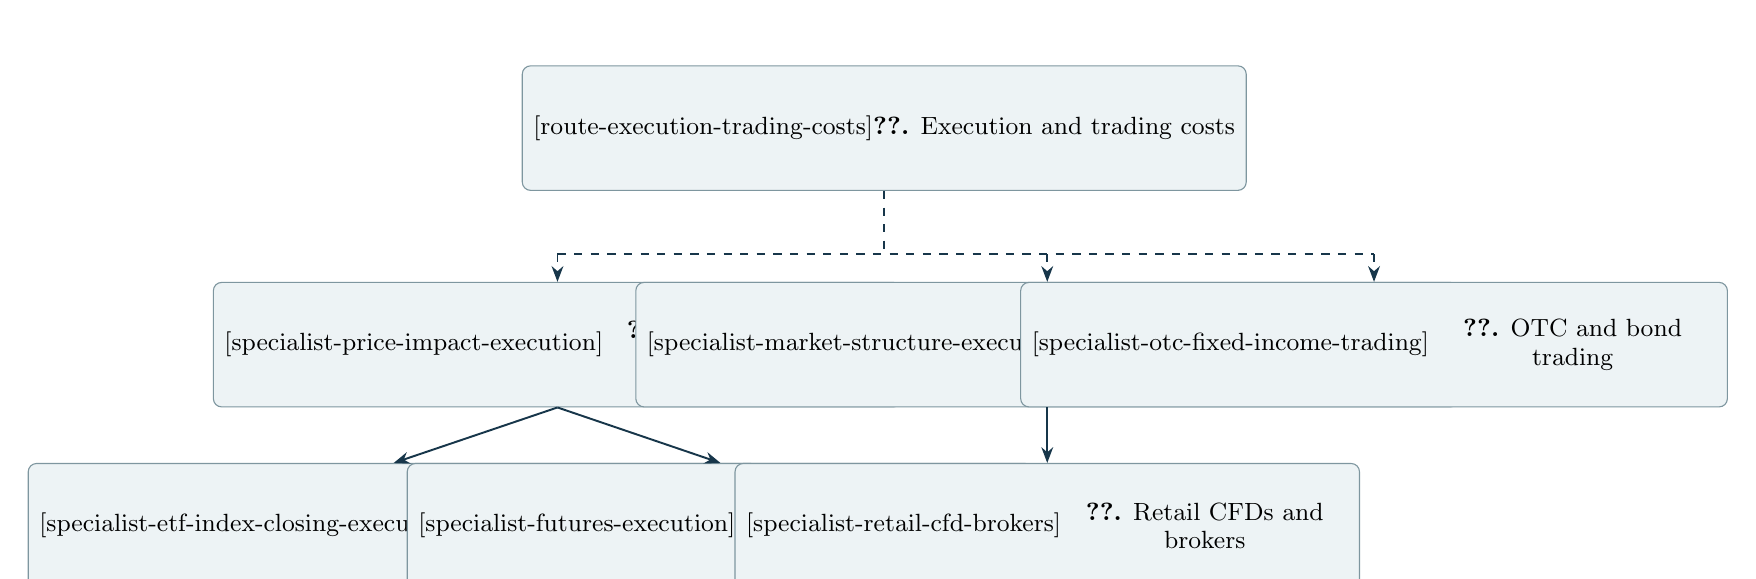
\begin{tikzpicture}[x=1cm,y=1cm]
\node[pathnode] (execution-trading-costs) at (6.23,0) {\MeasurePathNode{4.6cm}{\textbf{\ref*{route-execution-trading-costs}.} Execution and trading costs}\hyperref[route-execution-trading-costs]{\parbox[c][\pathnodeheight][c]{4.6cm}{\centering \textbf{\ref*{route-execution-trading-costs}.} Execution and trading costs}}};
\node[pathnode] (price-impact-execution) at (2.08,-2.75) {\MeasurePathNode{3.65cm}{\textbf{\ref*{specialist-price-impact-execution}.} Price impact and execution}\hyperref[specialist-price-impact-execution]{\parbox[c][\pathnodeheight][c]{3.65cm}{\centering \textbf{\ref*{specialist-price-impact-execution}.} Price impact and execution}}};
\node[pathnode] (market-structure-execution-quality) at (8.30,-2.75) {\MeasurePathNode{3.65cm}{\textbf{\ref*{specialist-market-structure-execution-quality}.} Rules, fees and execution quality}\hyperref[specialist-market-structure-execution-quality]{\parbox[c][\pathnodeheight][c]{3.65cm}{\centering \textbf{\ref*{specialist-market-structure-execution-quality}.} Rules, fees and execution quality}}};
\node[pathnode] (otc-fixed-income-trading) at (12.45,-2.75) {\MeasurePathNode{3.65cm}{\textbf{\ref*{specialist-otc-fixed-income-trading}.} OTC and bond trading}\hyperref[specialist-otc-fixed-income-trading]{\parbox[c][\pathnodeheight][c]{3.65cm}{\centering \textbf{\ref*{specialist-otc-fixed-income-trading}.} OTC and bond trading}}};
\node[pathnode] (etf-index-closing-execution) at (0.00,-5.05) {\MeasurePathNode{3.65cm}{\textbf{\ref*{specialist-etf-index-closing-execution}.} ETFs, index events and the close}\hyperref[specialist-etf-index-closing-execution]{\parbox[c][\pathnodeheight][c]{3.65cm}{\centering \textbf{\ref*{specialist-etf-index-closing-execution}.} ETFs, index events and the close}}};
\node[pathnode] (futures-execution) at (4.15,-5.05) {\MeasurePathNode{3.65cm}{\textbf{\ref*{specialist-futures-execution}.} Futures execution}\hyperref[specialist-futures-execution]{\parbox[c][\pathnodeheight][c]{3.65cm}{\centering \textbf{\ref*{specialist-futures-execution}.} Futures execution}}};
\node[pathnode] (retail-cfd-brokers) at (8.30,-5.05) {\MeasurePathNode{3.65cm}{\textbf{\ref*{specialist-retail-cfd-brokers}.} Retail CFDs and brokers}\hyperref[specialist-retail-cfd-brokers]{\parbox[c][\pathnodeheight][c]{3.65cm}{\centering \textbf{\ref*{specialist-retail-cfd-brokers}.} Retail CFDs and brokers}}};
\draw[entryline] (execution-trading-costs.south) -- (6.23,-1.60);
\draw[entryline] (2.08,-1.60) -- (12.45,-1.60);
\draw[entryarrow] (2.08,-1.60) -- (price-impact-execution.north);
\draw[entryarrow] (8.30,-1.60) -- (market-structure-execution-quality.north);
\draw[entryarrow] (12.45,-1.60) -- (otc-fixed-income-trading.north);
\draw[patharrow] (price-impact-execution.south) -- (etf-index-closing-execution.north);
\draw[patharrow] (price-impact-execution.south) -- (futures-execution.north);
\draw[patharrow] (market-structure-execution-quality.south) -- (retail-cfd-brokers.north);
\end{tikzpicture}\end{center}
\textbf{Overview checkpoint.} A section capstone: complete it after \hyperref[specialist-price-impact-execution]{\ref*{specialist-price-impact-execution}}, \hyperref[specialist-market-structure-execution-quality]{\ref*{specialist-market-structure-execution-quality}} and \hyperref[specialist-futures-execution]{\ref*{specialist-futures-execution}}.

\textbf{Bring these foundations with you.}\begin{itemize}
\item \hyperref[route-rates-credit-mortgages]{Rates: yield curves, term premia and derivatives} --- needed by \hyperref[specialist-otc-fixed-income-trading]{OTC and bond trading}.
\item \hyperref[route-corporate-credit-capital]{Corporate credit, hybrids and labelled bonds} --- needed by \hyperref[specialist-otc-fixed-income-trading]{OTC and bond trading}.
\item \hyperref[specialist-bond-swap-dealer-market-making]{Bond and swap dealing: RFQs, inventory and balance-sheet capacity} --- needed by \hyperref[specialist-otc-fixed-income-trading]{OTC and bond trading}.
\item \hyperref[specialist-fx-dealer-market-making]{FX dealing: internalisation, last look and hedging} --- needed by \hyperref[specialist-otc-fixed-income-trading]{OTC and bond trading}.
\item \hyperref[specialist-market-making-lob]{Market making, queues and limit-order-book models} --- needed by \hyperref[specialist-retail-cfd-brokers]{Retail CFDs and brokers}.
\end{itemize}\hyperref[learning-map]{Return to the whole-guide DAG.}
\Needspace{12\baselineskip}
\subsection{Price impact, optimal execution and TCA}\label{specialist-price-impact-execution}
\textbf{Specialist pathway.} In \hyperref[route-execution-trading-costs]{Execution, trading costs and market structure}.

\textbf{Outcome.} Estimate a price-impact model from executions, derive an optimal schedule and measure implementation shortfall with confidence intervals.

\textbf{Prerequisites.} Execution, trading costs and market structure overview; stochastic control basics.

\textbf{Review first.} \hyperref[route-execution-trading-costs]{Execution, trading costs and market structure}.

\textbf{Required readings, in order}
\begin{enumerate}\raggedright
\Needspace{5\baselineskip}\item \href{institutional_quantitative_finance_reading_list.pdf\#wide-perold-shortfall}{André F. Perold, ``The implementation shortfall: Paper versus reality''}\CataloguePage{160}\NoteKey{wide-perold-shortfall}\par \textbf{Foundations.} Define implementation shortfall.
\Needspace{5\baselineskip}\item \href{institutional_quantitative_finance_reading_list.pdf\#alpha-almgren}{Robert Almgren and Neil Chriss, ``Optimal Execution of Portfolio Transactions''}\CataloguePage{148}\NoteKey{alpha-almgren}\par \textbf{Theory.} Trade off impact cost and risk.
\Needspace{5\baselineskip}\item \href{institutional_quantitative_finance_reading_list.pdf\#catalogue-0500}{Anna A. Obizhaeva and Jiang Wang, ``Optimal Trading Strategy and Supply/Demand Dynamics''; author PDF}\CataloguePage{149}\NoteKey{catalogue-0500}\par \textbf{Theory.} Add order-book resilience.
\Needspace{5\baselineskip}\item \href{institutional_quantitative_finance_reading_list.pdf\#wide-almgren-direct-impact}{Robert Almgren, Chee Thum, Emmanuel Hauptmann and Hong Li, ``Direct Estimation of Equity Market Impact''}\CataloguePage{157}\NoteKey{wide-almgren-direct-impact}\par \textbf{Evidence.} Estimate impact from institutional orders.
\Needspace{5\baselineskip}\item \href{institutional_quantitative_finance_reading_list.pdf\#wide-toth-square-root}{Bence Tóth, Yves Lempérière, Cyril Deremble, Joachim de Lataillade, Julien Kockelkoren and Jean-Philippe Bouchaud, ``Anomalous Price Impact and the Critical Nature of Liquidity in Financial Markets''}\CataloguePage{157}\NoteKey{wide-toth-square-root}\par \textbf{Evidence.} Study the square-root law.
\Needspace{5\baselineskip}\item \href{institutional_quantitative_finance_reading_list.pdf\#wide-sato-kanazawa-sqrt}{Yuki Sato and Kiyoshi Kanazawa, ``Strict Universality of the Square-Root Law in Price Impact across Stocks: A Complete Survey of the Tokyo Stock Exchange''}\CataloguePage{157}\NoteKey{wide-sato-kanazawa-sqrt}\par \textbf{Evidence.} See account-level confirmation of the square-root exponent.
\Needspace{5\baselineskip}\item \href{institutional_quantitative_finance_reading_list.pdf\#wide-zarinelli-beyond-sqrt}{Elia Zarinelli, Michele Treccani, J. Doyne Farmer and Fabrizio Lillo, ``Beyond the square root: Evidence for logarithmic dependence of market impact on size and participation rate''}\CataloguePage{157}\NoteKey{wide-zarinelli-beyond-sqrt}\par \textbf{Counter-evidence.} Check log-like impact at large sizes.
\Needspace{5\baselineskip}\item \href{institutional_quantitative_finance_reading_list.pdf\#wide-bouchaud-propagator}{Jean-Philippe Bouchaud, Yuval Gefen, Marc Potters and Matteo Wyart, ``Fluctuations and response in financial markets: the subtle nature of random price changes''}\CataloguePage{157}\NoteKey{wide-bouchaud-propagator}\par \textbf{Methods.} Model transient impact with a propagator.
\Needspace{5\baselineskip}\item \href{institutional_quantitative_finance_reading_list.pdf\#catalogue-0501}{Jim Gatheral, ``No-Dynamic-Arbitrage and Market Impact''}\CataloguePage{149}\NoteKey{catalogue-0501}\par \textbf{Theory.} Rule out dynamic arbitrage in impact models.
\Needspace{5\baselineskip}\item \href{institutional_quantitative_finance_reading_list.pdf\#wide-alfonsi-transient}{Aurélien Alfonsi, Antje Fruth and Alexander Schied, ``Optimal execution strategies in limit order books with general shape functions''}\CataloguePage{157}\NoteKey{wide-alfonsi-transient}\par \textbf{Methods.} Optimise with resilient order books.
\Needspace{5\baselineskip}\item \href{institutional_quantitative_finance_reading_list.pdf\#wide-kyle-obizhaeva-invariance}{Albert S. Kyle and Anna A. Obizhaeva, ``Market Microstructure Invariance: Empirical Hypotheses''}\CataloguePage{157}\NoteKey{wide-kyle-obizhaeva-invariance}\par \textbf{Evidence.} Scale costs with invariance.
\Needspace{5\baselineskip}\item \href{institutional_quantitative_finance_reading_list.pdf\#wide-webster-price-impact}{Kevin T. Webster, \emph{Handbook of Price Impact Modeling}}\CataloguePage{157}\NoteKey{wide-webster-price-impact}\par \textbf{Implementation.} Fit impact models and avoid statistical biases.
\Needspace{5\baselineskip}\item \href{institutional_quantitative_finance_reading_list.pdf\#wide-bacry-life-cycle}{Emmanuel Bacry, Adrian Iuga, Matthieu Lasnier and Charles-Albert Lehalle, ``Market Impacts and the Life Cycle of Investors Orders''}\CataloguePage{160}\NoteKey{wide-bacry-life-cycle}\par \textbf{Evidence.} Measure impact decay after execution.
\Needspace{5\baselineskip}\item \href{institutional_quantitative_finance_reading_list.pdf\#catalogue-0504}{Andrea Frazzini, Ronen Israel and Tobias Moskowitz, ``Trading Costs''}\CataloguePage{149}\NoteKey{catalogue-0504}\par \textbf{Evidence.} Use live trading-cost estimates.
\Needspace{5\baselineskip}\item \href{institutional_quantitative_finance_reading_list.pdf\#w3-maitrier-double-sqrt}{Guillaume Maitrier, Grégoire Loeper, Kiyoshi Kanazawa and Jean-Philippe Bouchaud, ``The ‘double’ square-root law: evidence for the mechanical origin of market impact using Tokyo stock exchange data''}\CataloguePage{158}\NoteKey{w3-maitrier-double-sqrt}\par \textbf{Evidence.} Test the mechanical origin of square-root impact.
\end{enumerate}
\Needspace{5\baselineskip}\textbf{Checkpoint.} From parent-order executions (or a public metaorder proxy), fit square-root and propagator impact models with out-of-sample tests; compute an Almgren--Chriss schedule for a target order and report expected shortfall, its standard error and the effect of impact decay assumptions.

\textbf{Optional branches.} \href{institutional_quantitative_finance_reading_list.pdf\#wide-engle-ferstenberg-russell}{Measure execution risk as well as cost.}\BranchPage{160} \href{institutional_quantitative_finance_reading_list.pdf\#wide-kissell-methods}{Read a TCA and algorithm-design text.}\BranchPage{160} \href{institutional_quantitative_finance_reading_list.pdf\#w3-naviglio-metaorder-public}{Understand why public-data impact estimates mislead.}\BranchPage{158} \href{institutional_quantitative_finance_reading_list.pdf\#w3-abijaber-neuman-propagator}{Liquidate with signals and Volterra propagators.}\BranchPage{160} \href{institutional_quantitative_finance_reading_list.pdf\#w3-campbell-nutz-execution-game}{Model execution among many traders.}\BranchPage{160} \href{institutional_quantitative_finance_reading_list.pdf\#w4-bank-cartea-signals}{Trade on short-term order-flow signals under flow-driven impact.}\BranchPage{160}
\par{\small \hyperref[learning-map]{Learning pathway DAG} \textbar{} \hyperref[route-execution-trading-costs]{Section overview} \textbar{} \hyperref[map-execution-trading-costs]{Section DAG}\NoteKey{price-impact-execution}}
\Needspace{12\baselineskip}
\subsection{Market structure rules, fees and execution quality}\label{specialist-market-structure-execution-quality}
\textbf{Specialist pathway.} In \hyperref[route-execution-trading-costs]{Execution, trading costs and market structure}.

\textbf{Outcome.} Explain how fragmentation, dark trading, fees, tick size, odd lots, retail routing and trading hours affect execution quality, and track the 2024–2026 U.S. and EU rule changes.

\textbf{Prerequisites.} Execution, trading costs and market structure overview.

\textbf{Review first.} \hyperref[route-execution-trading-costs]{Execution, trading costs and market structure}.

\textbf{Required readings, in order}
\begin{enumerate}\raggedright
\Needspace{5\baselineskip}\item \href{institutional_quantitative_finance_reading_list.pdf\#wide-ohara-ye-fragmentation}{Maureen O'Hara and Mao Ye, ``Is market fragmentation harming market quality?''}\CataloguePage{150}\NoteKey{wide-ohara-ye-fragmentation}\par \textbf{Evidence.} Assess fragmentation effects.
\Needspace{5\baselineskip}\item \href{institutional_quantitative_finance_reading_list.pdf\#wide-zhu-dark-pools}{Haoxiang Zhu, ``Do Dark Pools Harm Price Discovery?''}\CataloguePage{151}\NoteKey{wide-zhu-dark-pools}\par \textbf{Theory.} Model dark-pool price discovery.
\Needspace{5\baselineskip}\item \href{institutional_quantitative_finance_reading_list.pdf\#ex-colliard-foucault-2012}{Jean-Edouard Colliard and Thierry Foucault, ``Trading Fees and Efficiency in Limit Order Markets''}\CataloguePage{152}\NoteKey{ex-colliard-foucault-2012}\par \textbf{Theory.} See how the level and maker–taker split of fees change limit-order fill rates and spreads.
\Needspace{5\baselineskip}\item \href{institutional_quantitative_finance_reading_list.pdf\#ex-malinova-park-2015}{Katya Malinova and Andreas Park, ``Subsidizing Liquidity: The Impact of Make/Take Fees on Market Quality''}\CataloguePage{152}\NoteKey{ex-malinova-park-2015}\par \textbf{Evidence.} Measure what a maker–taker fee change does to quotes, all-in costs and order aggressiveness.
\Needspace{5\baselineskip}\item \href{institutional_quantitative_finance_reading_list.pdf\#ex-battalio-corwin-jennings-2016}{Robert Battalio, Shane A. Corwin and Robert Jennings, ``Can Brokers Have It All? On the Relation between Make-Take Fees and Limit Order Execution Quality''}\CataloguePage{152}\NoteKey{ex-battalio-corwin-jennings-2016}\par \textbf{Evidence.} Test whether routing limit orders for rebates costs customers fills.
\Needspace{5\baselineskip}\item \href{institutional_quantitative_finance_reading_list.pdf\#w3-barardehi-tick-pilot}{Yashar H. Barardehi, Peter Dixon, Qiyu Liu and Ariel Lohr, ``When does the tick size help or harm market quality? Evidence from the Tick Size Pilot''}\CataloguePage{151}\NoteKey{w3-barardehi-tick-pilot}\par \textbf{Evidence.} Use Tick Size Pilot evidence on when a wider tick helps or harms market quality.
\Needspace{5\baselineskip}\item \href{institutional_quantitative_finance_reading_list.pdf\#ex-bartlett-mccrary-ohara-2025}{Robert P. Bartlett, Justin McCrary and Maureen O'Hara, ``The Market Inside the Market: Odd-Lot Quotes''}\CataloguePage{154}\NoteKey{ex-bartlett-mccrary-ohara-2025}\par \textbf{Evidence.} Find better-priced odd-lot quotes inside the NBBO and their role in price discovery.
\Needspace{5\baselineskip}\item \href{institutional_quantitative_finance_reading_list.pdf\#ex-sec-tick-access-2024}{U.S. Securities and Exchange Commission, Regulation NMS: Minimum Pricing Increments, Access Fees, and Transparency of Better Priced Orders (Release 34-101070); exemptive order on compliance dates (Press Release 2025-130)}\CataloguePage{156}\NoteKey{ex-sec-tick-access-2024}\par \textbf{Regulation.} Track the smaller tick, lower access-fee caps and odd-lot data rules, and their postponed dates.
\Needspace{5\baselineskip}\item \href{institutional_quantitative_finance_reading_list.pdf\#wide-bjzz-retail}{Ekkehart Boehmer, Charles M. Jones, Xiaoyan Zhang and Xinran Zhang, ``Tracking Retail Investor Activity''}\CataloguePage{152}\NoteKey{wide-bjzz-retail}\par \textbf{Data.} Identify retail trades in TAQ.
\Needspace{5\baselineskip}\item \href{institutional_quantitative_finance_reading_list.pdf\#wide-barber-subpenny}{Brad M. Barber, Xing Huang, Philippe Jorion, Terrance Odean and Christopher Schwarz, ``A (Sub)penny for Your Thoughts: Tracking Retail Investor Activity in TAQ''}\CataloguePage{152}\NoteKey{wide-barber-subpenny}\par \textbf{Counter-evidence.} See the BJZZ algorithm's misclassification.
\Needspace{5\baselineskip}\item \href{institutional_quantitative_finance_reading_list.pdf\#w3-dyhrberg-retail-execution}{Anne Haubo Dyhrberg, Andriy Shkilko and Ingrid M. Werner, ``The retail execution quality landscape''}\CataloguePage{153}\NoteKey{w3-dyhrberg-retail-execution}\par \textbf{Evidence.} Measure retail execution quality across wholesalers.
\Needspace{5\baselineskip}\item \href{institutional_quantitative_finance_reading_list.pdf\#ex-sec-rule605-2024}{U.S. Securities and Exchange Commission, Disclosure of Order Execution Information (Release 34-99679); compliance-date extension (Release 34-104147)}\CataloguePage{156}\NoteKey{ex-sec-rule605-2024}\par \textbf{Regulation.} Use the expanded execution-quality reports, required from August 2026.
\Needspace{5\baselineskip}\item \href{institutional_quantitative_finance_reading_list.pdf\#ex-sec-withdrawal-2025}{U.S. Securities and Exchange Commission, Withdrawal of Proposed Regulatory Actions (Release 34-103247)}\CataloguePage{156}\NoteKey{ex-sec-withdrawal-2025}\par \textbf{Regulation.} Note that the order-competition and best-execution proposals were withdrawn in 2025.
\Needspace{5\baselineskip}\item \href{institutional_quantitative_finance_reading_list.pdf\#ex-barclay-hendershott-2003}{Michael J. Barclay and Terrence Hendershott, ``Price Discovery and Trading After Hours''}\CataloguePage{154}\NoteKey{ex-barclay-hendershott-2003}\par \textbf{Evidence.} Benchmark price discovery and trading costs outside regular hours.
\Needspace{5\baselineskip}\item \href{institutional_quantitative_finance_reading_list.pdf\#ex-overnight-trading-2026}{U.S. Securities and Exchange Commission, order approving Nasdaq's 23-hour trading day (Release 34-105199); New York Stock Exchange, Extended-Hours Trading FAQs (version 4.0)}\CataloguePage{156}\NoteKey{ex-overnight-trading-2026}\par \textbf{Regulation.} Follow the move to 23-hour equity trading and the conditions on its launch.
\Needspace{5\baselineskip}\item \href{institutional_quantitative_finance_reading_list.pdf\#ex-eu-mifir-review-2024}{European Parliament and Council, Regulation (EU) 2024/791 amending Regulation (EU) No 600/2014 (MiFIR review); ESMA, Consolidated Tape Providers}\CataloguePage{156}\NoteKey{ex-eu-mifir-review-2024}\par \textbf{Regulation.} Compare the EU route: consolidated tapes and the ban on payment for order flow.
\end{enumerate}
\Needspace{5\baselineskip}\textbf{Checkpoint.} Take one month of Rule 605-style execution data for retail market orders in a set of stocks. Compute effective and realised spreads and price improvement by order size and venue type, then show how the comparison would change with a half-penny tick, a lower access-fee cap and odd-lot quotes inside the NBBO. Flag every conclusion that depends on a rule not yet in force.

\textbf{Optional branches.} \href{institutional_quantitative_finance_reading_list.pdf\#wide-schwarz-retail-price}{Compare retail execution prices across brokers.}\BranchPage{153} \href{institutional_quantitative_finance_reading_list.pdf\#w3-ernst-spatt-sun-auctions}{Evaluate order-by-order auctions for retail flow.}\BranchPage{153} \href{institutional_quantitative_finance_reading_list.pdf\#w3-brugler-dark-access}{Compare dark pools with and without HFT access.}\BranchPage{151}
\par{\small \hyperref[learning-map]{Learning pathway DAG} \textbar{} \hyperref[route-execution-trading-costs]{Section overview} \textbar{} \hyperref[map-execution-trading-costs]{Section DAG}\NoteKey{market-structure-execution-quality}}
\Needspace{12\baselineskip}
\subsection{Fixed-income and OTC electronic trading}\label{specialist-otc-fixed-income-trading}
\textbf{Specialist pathway.} In \hyperref[route-execution-trading-costs]{Execution, trading costs and market structure}.

\textbf{Outcome.} Measure what clients pay in bond, swap and FX dealer markets, and explain how RFQ and portfolio trading, transparency rules and dealer capacity change those costs.

\textbf{Prerequisites.} Execution, trading costs and market structure overview; rates and corporate-credit overviews; the bond, swap and FX dealing pathways.

\textbf{Review first.} \hyperref[route-execution-trading-costs]{Execution, trading costs and market structure}; \hyperref[route-rates-credit-mortgages]{Rates: yield curves, term premia and derivatives}; \hyperref[route-corporate-credit-capital]{Corporate credit, hybrids and labelled bonds}; \hyperref[specialist-bond-swap-dealer-market-making]{Bond and swap dealing: RFQs, inventory and balance-sheet capacity}; \hyperref[specialist-fx-dealer-market-making]{FX dealing: internalisation, last look and hedging}.

\textbf{Required readings, in order}
\begin{enumerate}\raggedright
\Needspace{5\baselineskip}\item \href{institutional_quantitative_finance_reading_list.pdf\#wide-dgp-otc}{Darrell Duffie, Nicolae Gârleanu and Lasse Heje Pedersen, ``Over-the-Counter Markets''}\CataloguePage{147}\NoteKey{wide-dgp-otc}\par \textbf{Theory.} Model search and bargaining in OTC markets.
\Needspace{5\baselineskip}\item \href{institutional_quantitative_finance_reading_list.pdf\#wide-duffie-dark-markets}{Darrell Duffie, \emph{Dark Markets: Asset Pricing and Information Transmission in Over-the-Counter Markets}}\CataloguePage{147}\NoteKey{wide-duffie-dark-markets}\par \textbf{Theory.} Study information percolation in dealer markets.
\Needspace{5\baselineskip}\item \href{institutional_quantitative_finance_reading_list.pdf\#wide-bsv-fi-survey}{Hendrik Bessembinder, Chester Spatt and Kumar Venkataraman, ``A Survey of the Microstructure of Fixed-Income Markets''}\CataloguePage{167}\NoteKey{wide-bsv-fi-survey}\par \textbf{Foundations.} Survey fixed-income microstructure.
\Needspace{5\baselineskip}\item \href{institutional_quantitative_finance_reading_list.pdf\#wide-edwards-harris-piwowar}{Amy K. Edwards, Lawrence E. Harris and Michael S. Piwowar, ``Corporate Bond Market Transaction Costs and Transparency''}\CataloguePage{168}\NoteKey{wide-edwards-harris-piwowar}\par \textbf{Evidence.} Measure bond costs and transparency effects.
\Needspace{5\baselineskip}\item \href{institutional_quantitative_finance_reading_list.pdf\#wide-hendershott-madhavan}{Terrence Hendershott and Ananth Madhavan, ``Click or Call? Auction versus Search in the Over-the-Counter Market''}\CataloguePage{168}\NoteKey{wide-hendershott-madhavan}\par \textbf{Evidence.} Compare electronic auctions with voice search.
\Needspace{5\baselineskip}\item \href{institutional_quantitative_finance_reading_list.pdf\#wide-ohara-zhou-electronic}{Maureen O'Hara and Xing (Alex) Zhou, ``The electronic evolution of corporate bond dealers''}\CataloguePage{167}\NoteKey{wide-ohara-zhou-electronic}\par \textbf{Evidence.} See dealers adapt to electronic trading.
\Needspace{5\baselineskip}\item \href{institutional_quantitative_finance_reading_list.pdf\#latest-pinter-search-frictions-2025}{Gábor Pintér, Semih Üslü and Jean-Charles Wijnandts, Comparing Search and Intermediation Frictions Across Markets; Earlier Bank of England version}\CataloguePage{147}\NoteKey{latest-pinter-search-frictions-2025}\par \textbf{Evidence.} Compare search frictions across markets.
\Needspace{5\baselineskip}\item \href{institutional_quantitative_finance_reading_list.pdf\#exp-eisfeldt-interdealer-capacity}{Andrea L. Eisfeldt, Bernard Herskovic, and Shuo Liu, Interdealer Price Dispersion and Intermediary Capacity}\CataloguePage{242}\NoteKey{exp-eisfeldt-interdealer-capacity}\par \textbf{Evidence.} Link price dispersion to dealer capacity.
\Needspace{5\baselineskip}\item \href{institutional_quantitative_finance_reading_list.pdf\#wide-li-ohara-portfolio-trading}{Jessica Li, Maureen O'Hara, Andreas C. Rapp and Xing (Alex) Zhou, ``Bond Market Illiquidity: Is Portfolio Trading the Solution?''}\CataloguePage{168}\NoteKey{wide-li-ohara-portfolio-trading}\par \textbf{Evidence.} Assess portfolio trading.
\Needspace{5\baselineskip}\item \href{institutional_quantitative_finance_reading_list.pdf\#wide-li-li-investor-composition}{Jian Li and Haiyue Yu, ``Investor Composition and the Liquidity Component in the U.S. Corporate Bond Market''}\CataloguePage{168}\NoteKey{wide-li-li-investor-composition}\par \textbf{Evidence.} Relate investor composition to liquidity.
\Needspace{5\baselineskip}\item \href{institutional_quantitative_finance_reading_list.pdf\#exp-fx-algos}{BIS Markets Committee, FX Execution Algorithms and Market Functioning}\CataloguePage{288}\NoteKey{exp-fx-algos}\par \textbf{Implementation.} Learn FX execution algorithms.
\Needspace{5\baselineskip}\item \href{institutional_quantitative_finance_reading_list.pdf\#w2-hendershott-relationship}{Terrence Hendershott, Dan Li, Dmitry Livdan and Norman Schürhoff, ``Relationship Trading in Over-the-Counter Markets''}\CataloguePage{168}\NoteKey{w2-hendershott-relationship}\par \textbf{Evidence.} See how dealer relationships shape costs.
\Needspace{5\baselineskip}\item \href{institutional_quantitative_finance_reading_list.pdf\#w2-ohara-zhou-covid}{Maureen O'Hara and Xing (Alex) Zhou, ``Anatomy of a liquidity crisis: Corporate bonds in the COVID-19 crisis''}\CataloguePage{168}\NoteKey{w2-ohara-zhou-covid}\par \textbf{Evidence.} Study the March 2020 bond liquidity collapse.
\Needspace{5\baselineskip}\item \href{institutional_quantitative_finance_reading_list.pdf\#w3-hendershott-quote-competition}{Terrence Hendershott, Dan Li, Dmitry Livdan, Norman Schürhoff and Kumar Venkataraman, ``Quote Competition in Corporate Bonds''}\CataloguePage{169}\NoteKey{w3-hendershott-quote-competition}\par \textbf{Evidence.} See how indicative quotes compete in corporate bonds.
\end{enumerate}
\Needspace{5\baselineskip}\textbf{Checkpoint.} From TRACE data, estimate round-trip costs by trade size and rating before and after a transparency or electronification change; compare RFQ, portfolio-trade and voice costs where identifiable, and document data limitations.

\textbf{Optional branches.} \href{institutional_quantitative_finance_reading_list.pdf\#wide-dick-nielsen-trace}{Clean Enhanced TRACE before measuring costs.}\BranchPage{520} \href{institutional_quantitative_finance_reading_list.pdf\#w2-kargar-covid}{Measure the price of immediacy in 2020.}\BranchPage{169} \href{institutional_quantitative_finance_reading_list.pdf\#w2-riggs-cds-swaps}{Study RFQ behaviour on swap execution facilities.}\BranchPage{169} \href{institutional_quantitative_finance_reading_list.pdf\#w3-kargar-sequential-search}{Unpack customer search on a bond platform.}\BranchPage{169} \href{institutional_quantitative_finance_reading_list.pdf\#w4-bjonnes-osler-otc-dispersion}{See OTC spread dispersion across client types.}\BranchPage{169} \href{institutional_quantitative_finance_reading_list.pdf\#w4-doan-etf-otc-transparency}{See ETF disclosure act as OTC price transparency.}\BranchPage{169} \href{institutional_quantitative_finance_reading_list.pdf\#w4-dynkin-systematic-credit}{Implement systematic credit portfolios.}\BranchPage{243}
\par{\small \hyperref[learning-map]{Learning pathway DAG} \textbar{} \hyperref[route-execution-trading-costs]{Section overview} \textbar{} \hyperref[map-execution-trading-costs]{Section DAG}\NoteKey{otc-fixed-income-trading}}
\Needspace{12\baselineskip}
\subsection{ETFs, index events and closing auctions}\label{specialist-etf-index-closing-execution}
\textbf{Specialist pathway.} In \hyperref[route-execution-trading-costs]{Execution, trading costs and market structure}.

\textbf{Outcome.} Plan trades around ETF creations, index reconstitutions and the closing auction, estimating price pressure, reversal and the cost borne by index funds.

\textbf{Prerequisites.} Price impact, optimal execution and TCA.

\textbf{Review first.} \hyperref[route-execution-trading-costs]{Execution, trading costs and market structure}; \hyperref[specialist-price-impact-execution]{Price impact, optimal execution and TCA}.

\textbf{Required readings, in order}
\begin{enumerate}\raggedright
\Needspace{5\baselineskip}\item \href{institutional_quantitative_finance_reading_list.pdf\#ex-lettau-madhavan-2018}{Martin Lettau and Ananth Madhavan, ``Exchange-Traded Funds 101 for Economists''}\CataloguePage{175}\NoteKey{ex-lettau-madhavan-2018}\par \textbf{Mechanics.} Learn ETF structure, creation and redemption before studying its trading.
\Needspace{5\baselineskip}\item \href{institutional_quantitative_finance_reading_list.pdf\#wide-pan-zeng-etf}{Kevin Pan and Yao Zeng, ``ETF Arbitrage Under Liquidity Mismatch''}\CataloguePage{202}\NoteKey{wide-pan-zeng-etf}\par \textbf{Theory.} See how authorised participants' dealer role limits arbitrage when the underlying is illiquid.
\Needspace{5\baselineskip}\item \href{institutional_quantitative_finance_reading_list.pdf\#ex-box-2021}{Travis Box, Ryan Davis, Richard Evans and Andrew Lynch, ``Intraday arbitrage between ETFs and their underlying portfolios''}\CataloguePage{175}\NoteKey{ex-box-2021}\par \textbf{Evidence.} Test whether ETF trading moves underlying prices intraday, or ETF quotes adjust instead.
\Needspace{5\baselineskip}\item \href{institutional_quantitative_finance_reading_list.pdf\#w3-evans-operational-shorting}{Richard B. Evans, Rabih Moussawi, Michael S. Pagano and John Sedunov, ``Operational shorting and ETF liquidity provision''}\CataloguePage{203}\NoteKey{w3-evans-operational-shorting}\par \textbf{Evidence.} See how operational shorting lets ETF liquidity providers sell before creating shares.
\Needspace{5\baselineskip}\item \href{institutional_quantitative_finance_reading_list.pdf\#exp-koont-bond-etf-liquidity}{Naz Koont, Yiming Ma, Lubos Pastor, and Yao Zeng, Steering a Ship in Illiquid Waters: Active Management of Passive Funds}\CataloguePage{242}\NoteKey{exp-koont-bond-etf-liquidity}\par \textbf{Evidence.} Follow how bond ETFs choose creation and redemption baskets.
\Needspace{5\baselineskip}\item \href{institutional_quantitative_finance_reading_list.pdf\#ex-shleifer-1986}{Andrei Shleifer, ``Do Demand Curves for Stocks Slope Down?''}\CataloguePage{175}\NoteKey{ex-shleifer-1986}\par \textbf{Evidence.} Start the index-inclusion evidence: returns tied to index-fund buying.
\Needspace{5\baselineskip}\item \href{institutional_quantitative_finance_reading_list.pdf\#ex-chen-noronha-singal-2004}{Honghui Chen, Gregory Noronha and Vijay Singal, ``The Price Response to S\&P 500 Index Additions and Deletions: Evidence of Asymmetry and a New Explanation''}\CataloguePage{175}\NoteKey{ex-chen-noronha-singal-2004}\par \textbf{Evidence.} Explain why additions and deletions have asymmetric price effects.
\Needspace{5\baselineskip}\item \href{institutional_quantitative_finance_reading_list.pdf\#ex-madhavan-2003}{Ananth Madhavan, ``The Russell Reconstitution Effect''}\CataloguePage{176}\NoteKey{ex-madhavan-2003}\par \textbf{Evidence.} Measure the Russell reconstitution effect and the cost and risk of supplying liquidity to it.
\Needspace{5\baselineskip}\item \href{institutional_quantitative_finance_reading_list.pdf\#ex-petajisto-2011}{Antti Petajisto, ``The index premium and its hidden cost for index funds''}\CataloguePage{176}\NoteKey{ex-petajisto-2011}\par \textbf{Evidence.} Estimate the index premium and its hidden turnover cost to index funds.
\Needspace{5\baselineskip}\item \href{institutional_quantitative_finance_reading_list.pdf\#wide-bogousslavsky-muravyev}{Vincent Bogousslavsky and Dmitriy Muravyev, ``Who trades at the close? Implications for price discovery and liquidity''}\CataloguePage{153}\NoteKey{wide-bogousslavsky-muravyev}\par \textbf{Evidence.} Identify who trades at the close and what that does to closing prices.
\Needspace{5\baselineskip}\item \href{institutional_quantitative_finance_reading_list.pdf\#ex-jegadeesh-wu-2022}{Narasimhan Jegadeesh and Yanbin Wu, ``Closing auctions: Nasdaq versus NYSE''}\CataloguePage{176}\NoteKey{ex-jegadeesh-wu-2022}\par \textbf{Evidence.} Compare closing-auction depth and impact decay on Nasdaq and the NYSE.
\Needspace{5\baselineskip}\item \href{institutional_quantitative_finance_reading_list.pdf\#ex-goyal-jegadeesh-wu-2026}{Amit Goyal, Narasimhan Jegadeesh and Yanbin Wu, ``Price Impact in Closing Auctions, Opening Auctions, and Continuous Markets: A Benchmark''}\CataloguePage{176}\NoteKey{ex-goyal-jegadeesh-wu-2026}\par \textbf{Implementation.} Route strategy trades to the cheaper auction or continuous mechanism and measure the saving.
\end{enumerate}
\Needspace{5\baselineskip}\textbf{Checkpoint.} Choose one index reconstitution. From announcement to effective date, measure abnormal returns, volume and closing-auction imbalance for added and deleted stocks. Compare executing an index fund's trades in the closing auction with a VWAP schedule over the prior week, reporting impact, reversal over the next five days and tracking error.

\textbf{Optional branches.} \href{institutional_quantitative_finance_reading_list.pdf\#ex-greenwood-2005}{Follow arbitrage dynamics after a large index-driven demand shock.}\BranchPage{176} \href{institutional_quantitative_finance_reading_list.pdf\#wide-ben-david-etf-review}{Survey ETF mechanics and their effects on underlying markets.}\BranchPage{202} \href{institutional_quantitative_finance_reading_list.pdf\#wide-brown-davies-ringgenberg}{Use creation and redemption flows as a signal of non-fundamental demand.}\BranchPage{202}
\par{\small \hyperref[learning-map]{Learning pathway DAG} \textbar{} \hyperref[route-execution-trading-costs]{Section overview} \textbar{} \hyperref[map-execution-trading-costs]{Section DAG}\NoteKey{etf-index-closing-execution}}
\Needspace{12\baselineskip}
\subsection{Futures execution: matching, rolls and settlement}\label{specialist-futures-execution}
\textbf{Specialist pathway.} In \hyperref[route-execution-trading-costs]{Execution, trading costs and market structure}.

\textbf{Outcome.} Execute futures orders and rolls using the contract's matching algorithm, settlement mechanisms and cross-market price discovery, and measure roll costs.

\textbf{Prerequisites.} Price impact, optimal execution and TCA; futures delivery and settlement mechanics.

\textbf{Review first.} \hyperref[route-execution-trading-costs]{Execution, trading costs and market structure}; \hyperref[specialist-price-impact-execution]{Price impact, optimal execution and TCA}.

\textbf{Required readings, in order}
\begin{enumerate}\raggedright
\Needspace{5\baselineskip}\item \href{institutional_quantitative_finance_reading_list.pdf\#w5-garbade-silber}{Kenneth D. Garbade and William L. Silber, ``Price Movements and Price Discovery in Futures and Cash Markets''}\CataloguePage{371}\NoteKey{w5-garbade-silber}\par \textbf{Foundations.} Model price discovery between futures and cash markets and the delivery link between them.
\Needspace{5\baselineskip}\item \href{institutional_quantitative_finance_reading_list.pdf\#ex-hasbrouck-2003}{Joel Hasbrouck, ``Intraday Price Formation in U.S. Equity Index Markets''}\CataloguePage{174}\NoteKey{ex-hasbrouck-2003}\par \textbf{Evidence.} Locate price discovery among E-minis, regular futures and ETFs.
\Needspace{5\baselineskip}\item \href{institutional_quantitative_finance_reading_list.pdf\#ex-cme-matching}{CME Group, CME Globex Matching Algorithms (Client Systems Wiki)}\CataloguePage{174}\NoteKey{ex-cme-matching}\par \textbf{Mechanics.} Check whether a contract matches by time priority or pro rata before modelling fills.
\Needspace{5\baselineskip}\item \href{institutional_quantitative_finance_reading_list.pdf\#ex-aspris-2015}{Angelo Aspris, Sean Foley, Drew Harris and Peter O'Neill, ``Time Pro-rata Matching: Evidence of a Change in LIFFE STIR Futures''}\CataloguePage{175}\NoteKey{ex-aspris-2015}\par \textbf{Evidence.} See how a switch from pure to time pro-rata matching changed depth and order sizing.
\Needspace{5\baselineskip}\item \href{institutional_quantitative_finance_reading_list.pdf\#w5-kirilenko-flash-crash}{Andrei Kirilenko, Albert S. Kyle, Mehrdad Samadi and Tugkan Tuzun, ``The Flash Crash: High-Frequency Trading in an Electronic Market''}\CataloguePage{537}\NoteKey{w5-kirilenko-flash-crash}\par \textbf{Evidence.} Study high-frequency trading and liquidity in E-mini futures under stress.
\Needspace{5\baselineskip}\item \href{institutional_quantitative_finance_reading_list.pdf\#gap-rates-treasury-futures-delivery}{CME Group, The Treasury Futures Delivery Process, Eighth Edition; CME conversion-factor detail}\CataloguePage{224}\NoteKey{gap-rates-treasury-futures-delivery}\par \textbf{Mechanics.} Follow the delivery process and conversion factors that shape Treasury futures roll timing.
\Needspace{5\baselineskip}\item \href{institutional_quantitative_finance_reading_list.pdf\#ex-bessembinder-2016}{Hendrik Bessembinder, Allen Carrion, Laura Tuttle and Kumar Venkataraman, ``Liquidity, resiliency and market quality around predictable trades: Theory and evidence''}\CataloguePage{175}\NoteKey{ex-bessembinder-2016}\par \textbf{Evidence.} Measure liquidity and resiliency around a large ETF's predictable futures roll.
\Needspace{5\baselineskip}\item \href{institutional_quantitative_finance_reading_list.pdf\#ex-mou-2010}{Yiqun Mou, ``Limits to Arbitrage and Commodity Index Investment: Front-Running the Goldman Roll''}\CataloguePage{175}\NoteKey{ex-mou-2010}\par \textbf{Evidence.} Study trading ahead of a commodity index's predictable roll.
\Needspace{5\baselineskip}\item \href{institutional_quantitative_finance_reading_list.pdf\#wide-tang-xiong-index}{Ke Tang and Wei Xiong, ``Index Investment and the Financialization of Commodities''}\CataloguePage{338}\NoteKey{wide-tang-xiong-index}\par \textbf{Evidence.} Relate index-investment flows to commodity futures co-movement.
\Needspace{5\baselineskip}\item \href{institutional_quantitative_finance_reading_list.pdf\#ex-pirrong-2023}{Craig Pirrong, ``Strategic trading and manipulation in trade at settlement contracts''}\CataloguePage{175}\NoteKey{ex-pirrong-2023}\par \textbf{Theory.} Assess strategic and manipulative trading around trade-at-settlement contracts.
\end{enumerate}
\Needspace{5\baselineskip}\textbf{Checkpoint.} For one futures contract, identify its Globex matching algorithm and estimate passive fill probability from queue position or allocation share. Then plan a calendar roll for a fixed position: compare rolling early, in the index roll window and through trade-at-settlement, measuring spread, impact, calendar-spread slippage and settlement-price risk.

\textbf{Optional branches.} \href{institutional_quantitative_finance_reading_list.pdf\#exp-barth-kahn-treasury-basis}{See how the Treasury cash-futures basis trade depends on futures execution and repo.}\BranchPage{180} \href{institutional_quantitative_finance_reading_list.pdf\#wide-cheng-xiong-financialization}{Review the financialisation evidence behind index-roll flows.}\BranchPage{338}
\par{\small \hyperref[learning-map]{Learning pathway DAG} \textbar{} \hyperref[route-execution-trading-costs]{Section overview} \textbar{} \hyperref[map-execution-trading-costs]{Section DAG}\NoteKey{futures-execution}}
\Needspace{12\baselineskip}
\subsection{Retail CFDs: leverage limits, broker risk and client outcomes}\label{specialist-retail-cfd-brokers}
\textbf{Specialist pathway.} In \hyperref[route-execution-trading-costs]{Execution, trading costs and market structure}.

\textbf{Outcome.} Explain how retail CFD providers price, margin and hedge client flow, measure client outcomes, and judge what leverage caps, margin close-out and negative balance protection change.

\textbf{Prerequisites.} Market making and inventory models; market-structure rules and retail execution quality.

\textbf{Review first.} \hyperref[specialist-market-making-lob]{Market making, queues and limit-order-book models}; \hyperref[specialist-market-structure-execution-quality]{Market structure rules, fees and execution quality}.

\textbf{Required readings, in order}
\begin{enumerate}\raggedright
\Needspace{5\baselineskip}\item \href{institutional_quantitative_finance_reading_list.pdf\#cfd-esma-intervention-2018}{European Securities and Markets Authority, ESMA agrees to prohibit binary options and restrict CFDs to protect retail investors}\CataloguePage{188}\NoteKey{cfd-esma-intervention-2018}\par \textbf{Regulation.} Read the EU leverage caps, close-out rule, negative balance protection and loss warning.
\Needspace{5\baselineskip}\item \href{institutional_quantitative_finance_reading_list.pdf\#cfd-fca-ps19-18}{Financial Conduct Authority, PS19/18: Restricting contract for difference products sold to retail clients}\CataloguePage{188}\NoteKey{cfd-fca-ps19-18}\par \textbf{Regulation.} Compare the UK permanent rules and their scope.
\Needspace{5\baselineskip}\item \href{institutional_quantitative_finance_reading_list.pdf\#cfd-asic-pio-2022}{Australian Securities and Investments Commission, ASIC's CFD product intervention order extended for five years (22-082MR) and Report 724}\CataloguePage{188}\NoteKey{cfd-asic-pio-2022}\par \textbf{Evidence.} Measure the change in retail losses after Australia's order.
\Needspace{5\baselineskip}\item \href{institutional_quantitative_finance_reading_list.pdf\#cfd-barber-taiwan-2009}{Brad M. Barber, Yi-Tsung Lee, Yu-Jane Liu and Terrance Odean, ``Just How Much Do Individual Investors Lose by Trading?''}\CataloguePage{189}\NoteKey{cfd-barber-taiwan-2009}\par \textbf{Evidence.} Benchmark retail trading losses in a full-market dataset.
\Needspace{5\baselineskip}\item \href{institutional_quantitative_finance_reading_list.pdf\#cfd-lee-choy-2014}{Adrian D. Lee and Shan Choy, ``Contracts for dummies? The performance of investors in contracts for difference''}\CataloguePage{189}\NoteKey{cfd-lee-choy-2014}\par \textbf{Evidence.} Measure the after-cost returns of exchange-listed CFD investors.
\Needspace{5\baselineskip}\item \href{institutional_quantitative_finance_reading_list.pdf\#cfd-peshev-2021}{Petar Peshev, ``Analyzing CFD Retail Investors' Performance in a Post MiFID II Environment''}\CataloguePage{189}\NoteKey{cfd-peshev-2021}\par \textbf{Evidence.} Link margin use to retail CFD returns after MiFID II.
\Needspace{5\baselineskip}\item \href{institutional_quantitative_finance_reading_list.pdf\#cfd-heimer-simsek-2019}{Rawley Heimer and Alp Simsek, ``Should retail investors' leverage be limited?''}\CataloguePage{189}\NoteKey{cfd-heimer-simsek-2019}\par \textbf{Evidence.} Estimate the effects of a retail leverage cap.
\Needspace{5\baselineskip}\item \href{institutional_quantitative_finance_reading_list.pdf\#cfd-heimer-imas-2022}{Rawley Z. Heimer and Alex Imas, ``Biased by Choice: How Financial Constraints Can Reduce Financial Mistakes''}\CataloguePage{189}\NoteKey{cfd-heimer-imas-2022}\par \textbf{Evidence.} See how leverage limits change retail trading mistakes.
\Needspace{5\baselineskip}\item \href{institutional_quantitative_finance_reading_list.pdf\#cfd-butz-oomen-2019}{M. Butz and R. Oomen, ``Internalisation by electronic FX spot dealers''}\CataloguePage{189}\NoteKey{cfd-butz-oomen-2019}\par \textbf{Implementation.} Model when a dealer internalises or hedges client flow.
\Needspace{5\baselineskip}\item \href{institutional_quantitative_finance_reading_list.pdf\#w3-nutz-webster-warehouse}{Marcel Nutz, Kevin Webster and Long Zhao, ``Unwinding Stochastic Order Flow: When to Warehouse Trades''}\CataloguePage{164}\NoteKey{w3-nutz-webster-warehouse}\par \textbf{Methods.} Decide when to warehouse client flow and when to route it to market.
\Needspace{5\baselineskip}\item \href{institutional_quantitative_finance_reading_list.pdf\#w4-cartea-broker-informed}{Álvaro Cartea and Leandro Sánchez-Betancourt, ``Brokers and Informed Traders: Dealing with Toxic Flow and Extracting Trading Signals''}\CataloguePage{164}\NoteKey{w4-cartea-broker-informed}\par \textbf{Methods.} Separate informed from noise flow in a broker's book.
\Needspace{5\baselineskip}\item \href{institutional_quantitative_finance_reading_list.pdf\#w3-cartea-toxic-flow}{Álvaro Cartea, Gerardo Duran-Martin and Leandro Sánchez-Betancourt, ``Detecting toxic flow''}\CataloguePage{164}\NoteKey{w3-cartea-toxic-flow}\par \textbf{Methods.} Score client flow for toxicity before internalising it.
\Needspace{5\baselineskip}\item \href{institutional_quantitative_finance_reading_list.pdf\#cfd-andrade-demo-apps-2025}{Maira Andrade, Daniel Costa, Leonardo Weiss-Cohen, Jamie Torrance and Philip Newall, ``Trading is a losing game: an audit of deceptive choice architecture in demo-mode Contract for Difference (CFD) trading apps''}\CataloguePage{189}\NoteKey{cfd-andrade-demo-apps-2025}\par \textbf{Evidence.} Audit risk warnings and demo-mode design in CFD apps.
\end{enumerate}
\Needspace{5\baselineskip}\textbf{Checkpoint.} Using a published loss-disclosure percentage and a simulated client book, model a CFD provider that warehouses some client trades (B-book) and hedges the rest in the market (A-book). Show how leverage caps, the 50 percent close-out rule and negative balance protection change client loss distributions, provider revenue and provider tail risk. Route clients by a toxicity score and compare outcomes. State which results need proprietary client data.

\textbf{Optional branches.} \href{institutional_quantitative_finance_reading_list.pdf\#cfd-chapkovski-gamification-2026}{Test how gamified app features change trading.}\BranchPage{190} \href{institutional_quantitative_finance_reading_list.pdf\#roadmap-perpetual-fundamentals}{Compare CFD funding with perpetual-futures funding.}\BranchPage{446}
\par{\small \hyperref[learning-map]{Learning pathway DAG} \textbar{} \hyperref[route-execution-trading-costs]{Section overview} \textbar{} \hyperref[map-execution-trading-costs]{Section DAG}\NoteKey{retail-cfd-brokers}}
\clearpage
\part{Energy and commodities}\label{part-energy-commodities}
Study storage, curves, hedging and options, then spot price formation, market integration and long-run prices, physical delivery, price discovery and trading, commodity risk premia, factor strategies and allocation, oil-price shocks, forecasting and their macro-financial effects, gas hubs and network-constrained power markets, and emissions trading, carbon credits and certificates.

\textbf{Sections in learning order}\begin{enumerate}
\item[\ref*{route-energy-commodities}.] \hyperref[route-energy-commodities]{Commodity futures: storage, curves, hedging and options} --- Start with the theory of storage. Term-structure models build on it and lead to options and real options; hedging also builds on storage theory. Spot price formation, market integration and long-run prices follow in the next section, then physical delivery, price discovery, individual markets and trading firms.
\item[\ref*{route-commodity-spot-markets}.] \hyperref[route-commodity-spot-markets]{Commodity spot markets: price formation, market integration and long-run prices} --- Spot price assessment, spatial arbitrage and price cycles are separate entry points. Price stabilisation and trade policy build on spatial arbitrage; long-run prices build on price cycles. Physical delivery, price discovery, individual markets and trading firms follow in the next section and use these benchmarks and location spreads.
\item[\ref*{route-physical-commodity-markets}.] \hyperref[route-physical-commodity-markets]{Physical commodity markets: delivery, price discovery and trading} --- Start with contract design and delivery: metals, agriculture and crude oil build on it. Price discovery and fundamental data, freight, and trading firms and margin stress are separate entry points; freight and trading firms also need hedging (20.3). Risk premia and commodity investing follow in the next section, and oil-price shocks in the one after.
\item[\ref*{route-commodity-investing-premia}.] \hyperref[route-commodity-investing-premia]{Commodity risk premia and investing: factors, allocation and index products} --- Start with the risk premia in commodity futures (23.1). Factor strategies (23.2), the financialisation evidence (23.3) and strategic allocation (23.4) build on them, and index and ETF implementation (23.5) follows allocation. Oil-price shocks, forecasting and their macroeconomic and asset-price effects follow in the next section, then gas and power markets and environmental markets.
\item[\ref*{route-oil-shocks-macro}.] \hyperref[route-oil-shocks-macro]{Oil-price shocks, forecasting and the macroeconomy} --- Start with structural identification (24.1): forecasting (24.2), the macroeconomic transmission of oil shocks (24.3) and their effects on asset prices (24.4) all use the shocks it identifies. Forecasting also uses the futures risk premia of 23.1. Gas and power markets follow in the next section, then environmental markets.
\item[\ref*{route-power-gas-environmental}.] \hyperref[route-power-gas-environmental]{Gas and power markets: hubs, storage, networks and market design} --- Start with gas hub pricing and market integration (25.1), then value storage, transport and LNG options (25.2). Power networks and transmission rights (25.3) come before market design (25.4), renewable value (25.5), price modelling and forecasting (25.6) and short-term markets and flexibility (25.7). Environmental markets follow in the next section.
\item[\ref*{route-environmental-markets}.] \hyperref[route-environmental-markets]{Environmental markets: emissions trading, carbon credits and certificates} --- Start with cap-and-trade design (26.1). Allowance prices and derivatives (26.2), cost pass-through and leakage (26.3), voluntary carbon and biodiversity credits (26.4) and renewable certificates and fuel credits (26.5) all build on it.
\end{enumerate}
\hyperref[learning-map]{Return to the learning pathway DAG.}
\clearpage
\section{Commodity futures: storage, curves, hedging and options}\label{route-energy-commodities}
\label{route-9}
\textbf{Learning sequence.} Start with the theory of storage. Term-structure models build on it and lead to options and real options; hedging also builds on storage theory. Spot price formation, market integration and long-run prices follow in the next section, then physical delivery, price discovery, individual markets and trading firms.

\textbf{Section goals.} Across its pathways, this section teaches you to:
\begin{itemize}[leftmargin=1.4em,itemsep=0pt,topsep=1pt]
\item explain forward curves from inventories and convenience yield and estimate the storage model (\hyperref[specialist-commodity-storage-curves]{\ref*{specialist-commodity-storage-curves}})
\item fit factor, seasonal and jump models to futures curves (\hyperref[specialist-commodity-curve-models]{\ref*{specialist-commodity-curve-models}})
\item size and roll hedges of physical exposure (\hyperref[specialist-commodity-hedging]{\ref*{specialist-commodity-hedging}})
\item price commodity, spread and swing options and value real options (\hyperref[specialist-commodity-options-real-options]{\ref*{specialist-commodity-options-real-options}})
\end{itemize}
\textbf{Overview outcome.} Read a commodity futures curve through the theory of storage: compute the interest-adjusted basis, implied convenience yield and roll return, split a futures position's return into spot and roll, and judge a calendar-spread hedge of physical inventory.

\textbf{Prerequisites.} Common toolkit; forwards and futures, inventory accounting and basic constrained optimisation.

\textbf{Review first.} \hyperref[route-common-toolkit]{Common toolkit}.

\textbf{Required readings, in order}
\begin{enumerate}\raggedright
\Needspace{5\baselineskip}\item \href{institutional_quantitative_finance_reading_list.pdf\#exp-pindyck-commodity-physical-primer}{Robert S. Pindyck, The Dynamics of Commodity Spot and Futures Markets: A Primer}\CataloguePage{318}\NoteKey{exp-pindyck-commodity-physical-primer}\par Ground spot and futures prices in production, inventories and physical scarcity.
\Needspace{5\baselineskip}\item \href{institutional_quantitative_finance_reading_list.pdf\#exp-routledge-seppi-spatt-storage-curves}{Bryan R. Routledge, Duane J. Seppi, and Chester S. Spatt, Equilibrium Forward Curves for Commodities; author-hosted original article PDF}\CataloguePage{318}\NoteKey{exp-routledge-seppi-spatt-storage-curves}\par Connect storage economics to the shape and dynamics of forward curves.
\Needspace{5\baselineskip}\item \href{institutional_quantitative_finance_reading_list.pdf\#ec-fama-french-1987}{Eugene F. Fama and Kenneth R. French, ``Commodity Futures Prices: Some Evidence on Forecast Power, Premiums, and the Theory of Storage''}\CataloguePage{331}\NoteKey{ec-fama-french-1987}\par Test storage theory against a risk-premium reading of the basis across 21 commodities before choosing a pathway.
\Needspace{5\baselineskip}\item \href{institutional_quantitative_finance_reading_list.pdf\#physical-geman-commodities-2005}{Hélyette Geman, Commodities and Commodity Derivatives: Modeling and Pricing for Agriculturals, Metals and Energy}\CataloguePage{318}\NoteKey{physical-geman-commodities-2005}\par\emph{Selection:} Chapters on commodity markets, storage and forward curves; the metals and agriculture chapters support 22.2 and 22.3.\par Get one framework for storage, forward curves and derivatives across agricultural, metal and energy markets before specialising.
\end{enumerate}
\Needspace{5\baselineskip}\textbf{Checkpoint.} Choose one storable commodity and download its futures curve on two dates, one in contango and one in backwardation. Compute the interest-adjusted basis, implied convenience yield and annualised roll return on each date, split a one-year futures position's return into spot and roll, and show how a calendar-spread hedge of a physical inventory performs between the two dates.

\textbf{Optional branches.} \href{institutional_quantitative_finance_reading_list.pdf\#w5-pirrong-commodity-dynamics}{Solve structural storage models numerically before the specialist pathways.}\BranchPage{320}
\par\textbf{Continue in this section.} \hyperref[specialist-commodity-storage-curves]{Theory of storage, convenience yield and inventories}; \hyperref[specialist-commodity-curve-models]{Commodity term-structure models: factor, seasonal and jump models}; \hyperref[specialist-commodity-hedging]{Commodity hedging: hedge ratios, rolling hedges and corporate risk management}; \hyperref[specialist-commodity-options-real-options]{Commodity options, spread options and real options}.
\par{\small \hyperref[learning-map]{Learning pathway DAG} \textbar{} \hyperref[map-energy-commodities]{Section DAG}\NoteKey{energy-commodities}}
\clearpage
\subsection*{Commodity futures: storage, curves, hedging and options: pathway DAG}\phantomsection\label{map-energy-commodities}
\addcontentsline{toc}{subsection}{Commodity futures: storage, curves, hedging and options: pathway DAG}
Start with the section overview's readings, for orientation. Solid arrows show prerequisites within this section. Dashed connectors identify entry points with no further prerequisite in this section; the linked foundations below still apply. Follow the arrows for dependencies and the subsection numbers for reading order. Every node is clickable.
\begin{center}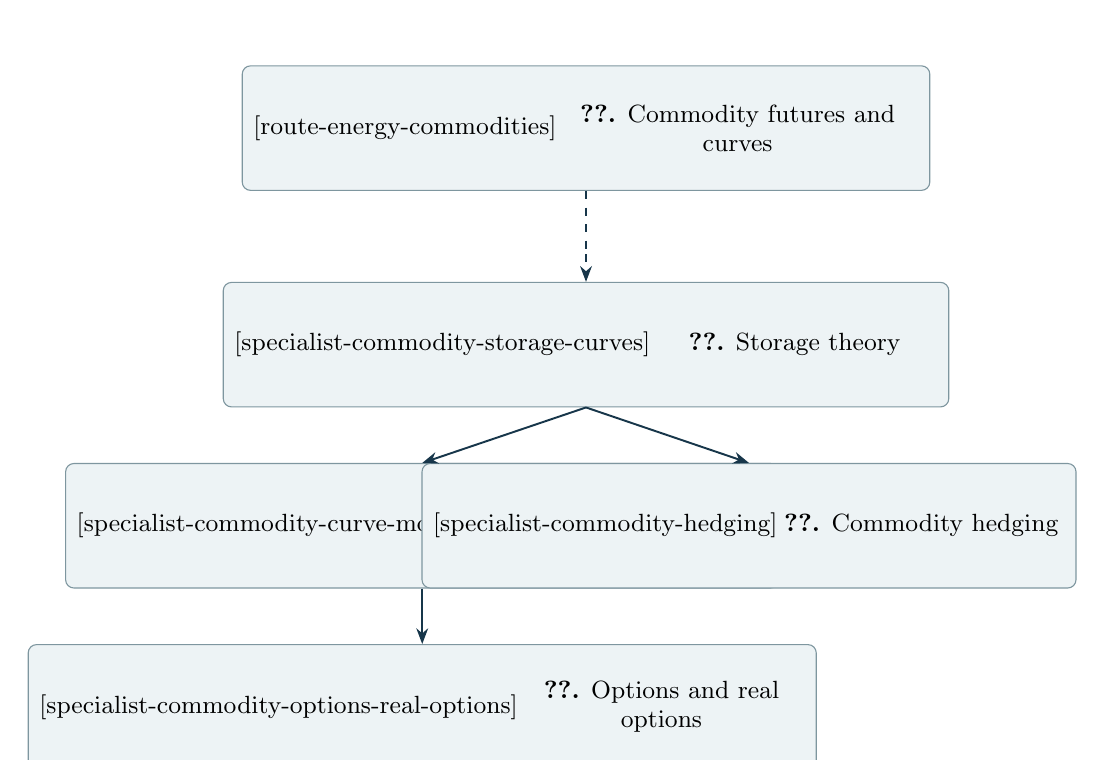
\begin{tikzpicture}[x=1cm,y=1cm]
\node[pathnode] (energy-commodities) at (2.08,0) {\MeasurePathNode{4.6cm}{\textbf{\ref*{route-energy-commodities}.} Commodity futures and curves}\hyperref[route-energy-commodities]{\parbox[c][\pathnodeheight][c]{4.6cm}{\centering \textbf{\ref*{route-energy-commodities}.} Commodity futures and curves}}};
\node[pathnode] (commodity-storage-curves) at (2.08,-2.75) {\MeasurePathNode{3.65cm}{\textbf{\ref*{specialist-commodity-storage-curves}.} Storage theory}\hyperref[specialist-commodity-storage-curves]{\parbox[c][\pathnodeheight][c]{3.65cm}{\centering \textbf{\ref*{specialist-commodity-storage-curves}.} Storage theory}}};
\node[pathnode] (commodity-curve-models) at (0.00,-5.05) {\MeasurePathNode{3.65cm}{\textbf{\ref*{specialist-commodity-curve-models}.} Curve models}\hyperref[specialist-commodity-curve-models]{\parbox[c][\pathnodeheight][c]{3.65cm}{\centering \textbf{\ref*{specialist-commodity-curve-models}.} Curve models}}};
\node[pathnode] (commodity-hedging) at (4.15,-5.05) {\MeasurePathNode{3.65cm}{\textbf{\ref*{specialist-commodity-hedging}.} Commodity hedging}\hyperref[specialist-commodity-hedging]{\parbox[c][\pathnodeheight][c]{3.65cm}{\centering \textbf{\ref*{specialist-commodity-hedging}.} Commodity hedging}}};
\node[pathnode] (commodity-options-real-options) at (0.00,-7.35) {\MeasurePathNode{3.65cm}{\textbf{\ref*{specialist-commodity-options-real-options}.} Options and real options}\hyperref[specialist-commodity-options-real-options]{\parbox[c][\pathnodeheight][c]{3.65cm}{\centering \textbf{\ref*{specialist-commodity-options-real-options}.} Options and real options}}};
\draw[entryline] (energy-commodities.south) -- (2.08,-1.60);
\draw[entryline] (2.08,-1.60) -- (2.08,-1.60);
\draw[entryarrow] (2.08,-1.60) -- (commodity-storage-curves.north);
\draw[patharrow] (commodity-storage-curves.south) -- (commodity-curve-models.north);
\draw[patharrow] (commodity-storage-curves.south) -- (commodity-hedging.north);
\draw[patharrow] (commodity-curve-models.south) -- (commodity-options-real-options.north);
\end{tikzpicture}\end{center}
\textbf{Bring these foundations with you.}\begin{itemize}
\item \hyperref[route-volatility-options]{Option pricing, volatility models and hedging} --- needed by \hyperref[specialist-commodity-options-real-options]{Options and real options}.
\end{itemize}\hyperref[learning-map]{Return to the whole-guide DAG.}
\Needspace{12\baselineskip}
\subsection{Theory of storage, convenience yield and inventories}\label{specialist-commodity-storage-curves}
\textbf{Specialist pathway.} In \hyperref[route-energy-commodities]{Commodity futures: storage, curves, hedging and options}.

\textbf{Outcome.} Explain the basis and the shape of commodity forward curves from inventories, convenience yield and stock-out risk; estimate the competitive storage model; and tell when backwardation reflects scarcity rather than a risk premium.

\textbf{Prerequisites.} Commodity futures: storage, curves, hedging and options overview; cost-of-carry pricing, dynamic programming and basic econometrics.

\textbf{Review first.} \hyperref[route-energy-commodities]{Commodity futures: storage, curves, hedging and options}.

\textbf{Required readings, in order}
\begin{enumerate}\raggedright
\Needspace{5\baselineskip}\item \href{institutional_quantitative_finance_reading_list.pdf\#ec-kaldor-1939}{Nicholas Kaldor, ``Speculation and Economic Stability''}\CataloguePage{330}\NoteKey{ec-kaldor-1939}\par \textbf{Foundations.} Read the origin of convenience yield: why holders of stocks accept a return below interest and storage costs.
\Needspace{5\baselineskip}\item \href{institutional_quantitative_finance_reading_list.pdf\#ec-working-1948}{Holbrook Working, ``Theory of the Inverse Carrying Charge in Futures Markets''}\CataloguePage{330}\NoteKey{ec-working-1948}\par \textbf{Foundations.} See why inverse carrying charges persist while stocks are positive, and why the price of storage depends on inventory.
\Needspace{5\baselineskip}\item \href{institutional_quantitative_finance_reading_list.pdf\#ec-brennan-1958}{Michael J. Brennan, ``The Supply of Storage''}\CataloguePage{331}\NoteKey{ec-brennan-1958}\par\emph{Selection:} The DOI is for the 1976 reprint (pages 100--107); the full article is in the American Economic Review, 1958.\par \textbf{Theory.} Derive the supply-of-storage curve: marginal storage cost net of convenience yield rises with stocks.
\Needspace{5\baselineskip}\item \href{institutional_quantitative_finance_reading_list.pdf\#ec-fama-french-1987}{Eugene F. Fama and Kenneth R. French, ``Commodity Futures Prices: Some Evidence on Forecast Power, Premiums, and the Theory of Storage''}\CataloguePage{331}\NoteKey{ec-fama-french-1987}\par \textbf{Evidence.} Test whether the basis varies with interest rates, storage costs and convenience yield, and whether it forecasts spot prices.
\Needspace{5\baselineskip}\item \href{institutional_quantitative_finance_reading_list.pdf\#ec-williams-wright-1991}{Jeffrey C. Williams and Brian D. Wright, \emph{Storage and Commodity Markets}}\CataloguePage{331}\NoteKey{ec-williams-wright-1991}\par \textbf{Theory.} Work through competitive storage with non-negative stocks and the nonlinear price dynamics it implies.
\Needspace{5\baselineskip}\item \href{institutional_quantitative_finance_reading_list.pdf\#physical-deaton-laroque-storage-1992}{Angus Deaton and Guy Laroque, On the Behaviour of Commodity Prices}\CataloguePage{319}\NoteKey{physical-deaton-laroque-storage-1992}\par \textbf{Evidence.} Confront the competitive-storage model with skewed and autocorrelated commodity prices.
\Needspace{5\baselineskip}\item \href{institutional_quantitative_finance_reading_list.pdf\#ec-deaton-laroque-1996}{Angus Deaton and Guy Laroque, ``Competitive Storage and Commodity Price Dynamics''}\CataloguePage{331}\NoteKey{ec-deaton-laroque-1996}\par \textbf{Evidence.} Estimate the storage model and see why it understates the autocorrelation of prices.
\Needspace{5\baselineskip}\item \href{institutional_quantitative_finance_reading_list.pdf\#cf-cafiero-2011}{Carlo Cafiero, Eugenio S. A. Bobenrieth H., Juan R. A. Bobenrieth H. and Brian D. Wright, ``The Empirical Relevance of the Competitive Storage Model''}\CataloguePage{332}\NoteKey{cf-cafiero-2011}\par \textbf{Counter-evidence.} See that a finer numerical solution lets the storage model match the autocorrelation of prices after all.
\Needspace{5\baselineskip}\item \href{institutional_quantitative_finance_reading_list.pdf\#ec-ng-pirrong-1994}{Victor K. Ng and Stephen Craig Pirrong, ``Fundamentals and Volatility: Storage, Spreads, and the Dynamics of Metals Prices''}\CataloguePage{331}\NoteKey{ec-ng-pirrong-1994}\par \textbf{Evidence.} Link spreads, inventories and volatility in industrial metals: low stocks mean steep backwardation and volatile spot prices.
\Needspace{5\baselineskip}\item \href{institutional_quantitative_finance_reading_list.pdf\#ec-pindyck-1994}{Robert S. Pindyck, ``Inventories and the Short-Run Dynamics of Commodity Prices''}\CataloguePage{331}\NoteKey{ec-pindyck-1994}\par \textbf{Evidence.} Estimate the marginal convenience yield from inventories in copper, heating oil and lumber.
\Needspace{5\baselineskip}\item \href{institutional_quantitative_finance_reading_list.pdf\#cf-symeonidis-2012}{Lazaros Symeonidis, Marcel Prokopczuk, Chris Brooks and Emese Lazar, ``Futures Basis, Inventory and Commodity Price Volatility: An Empirical Analysis''}\CataloguePage{332}\NoteKey{cf-symeonidis-2012}\par \textbf{Evidence.} Check across 21 commodities that low inventories mean backwardation and higher volatility.
\end{enumerate}
\Needspace{5\baselineskip}\textbf{Checkpoint.} Take daily settlements for the first twelve contracts of one storable commodity (WTI, copper or soybeans) for at least ten years, with weekly or monthly inventories. Compute the interest-adjusted basis and plot it against inventories to trace a supply-of-storage curve. Test whether spot volatility rises as inventories fall, and simulate a competitive storage model with stock-outs to compare its price autocorrelation and skewness with the data.

\textbf{Optional branches.} \href{institutional_quantitative_finance_reading_list.pdf\#ec-litzenberger-rabinowitz-1995}{Explain oil backwardation with the production options embedded in reserves.}\BranchPage{332} \href{institutional_quantitative_finance_reading_list.pdf\#ec-kogan-livdan-yaron-2009}{See how investment constraints shape the volatility of oil futures across maturities.}\BranchPage{332} \href{institutional_quantitative_finance_reading_list.pdf\#cf-gouel-legrand-2017}{Estimate the storage model with a trend in prices and recover occasional stock-outs.}\BranchPage{332} \href{institutional_quantitative_finance_reading_list.pdf\#catalogue-0242}{Link inventories and the basis to futures risk premia, studied further in 23.1.}\BranchPage{322}
\par{\small \hyperref[learning-map]{Learning pathway DAG} \textbar{} \hyperref[route-energy-commodities]{Section overview} \textbar{} \hyperref[map-energy-commodities]{Section DAG}\NoteKey{commodity-storage-curves}}
\Needspace{12\baselineskip}
\subsection{Commodity term-structure models: factor, seasonal and jump models}\label{specialist-commodity-curve-models}
\textbf{Specialist pathway.} In \hyperref[route-energy-commodities]{Commodity futures: storage, curves, hedging and options}.

\textbf{Outcome.} Fit one- to N-factor spot and convenience-yield models to a commodity futures curve by Kalman filter, add seasonality and jumps, calibrate to today's curve and volatilities, and judge what a fitted model implies for expected spot prices.

\textbf{Prerequisites.} Theory of storage, convenience yield and inventories (20.1); mean-reverting diffusions, Kalman filtering and affine pricing.

\textbf{Review first.} \hyperref[specialist-commodity-storage-curves]{Theory of storage, convenience yield and inventories}.

\textbf{Required readings, in order}
\begin{enumerate}\raggedright
\Needspace{5\baselineskip}\item \href{institutional_quantitative_finance_reading_list.pdf\#physical-gibson-schwartz-oil-1990}{Rajna Gibson and Eduardo S. Schwartz, Stochastic Convenience Yield and the Pricing of Oil Contingent Claims}\CataloguePage{318}\NoteKey{physical-gibson-schwartz-oil-1990}\par \textbf{Valuation.} Model spot price and a mean-reverting convenience yield jointly to price oil claims.
\Needspace{5\baselineskip}\item \href{institutional_quantitative_finance_reading_list.pdf\#physical-schwartz-three-models-1997}{Eduardo S. Schwartz, The Stochastic Behavior of Commodity Prices: Implications for Valuation and Hedging}\CataloguePage{318}\NoteKey{physical-schwartz-three-models-1997}\par \textbf{Valuation.} Compare one-, two- and three-factor models fitted to oil, copper and gold futures.
\Needspace{5\baselineskip}\item \href{institutional_quantitative_finance_reading_list.pdf\#cf-bessembinder-1995}{Hendrik Bessembinder, Jay F. Coughenour, Paul J. Seguin and Margaret Monroe Smoller, ``Mean Reversion in Equilibrium Asset Prices: Evidence from the Futures Term Structure''}\CataloguePage{332}\NoteKey{cf-bessembinder-1995}\par \textbf{Evidence.} Read the mean reversion that investors expect from the slope of the futures curve, by market.
\Needspace{5\baselineskip}\item \href{institutional_quantitative_finance_reading_list.pdf\#ec-schwartz-smith-2000}{Eduardo Schwartz and James E. Smith, ``Short-Term Variations and Long-Term Dynamics in Commodity Prices''}\CataloguePage{331}\NoteKey{ec-schwartz-smith-2000}\par \textbf{Valuation.} Recast the two-factor model as short-term deviations and a long-term equilibrium level, estimated by Kalman filter.
\Needspace{5\baselineskip}\item \href{institutional_quantitative_finance_reading_list.pdf\#ec-casassus-collin-dufresne-2005}{Jaime Casassus and Pierre Collin-Dufresne, ``Stochastic Convenience Yield Implied from Commodity Futures and Interest Rates''}\CataloguePage{332}\NoteKey{ec-casassus-collin-dufresne-2005}\par \textbf{Valuation.} Let convenience yield depend on spot prices and interest rates in a three-factor affine model and read off time-varying risk premia.
\Needspace{5\baselineskip}\item \href{institutional_quantitative_finance_reading_list.pdf\#cf-cortazar-naranjo-2006}{Gonzalo Cortazar and Lorenzo Naranjo, ``An N-Factor Gaussian Model of Oil Futures Prices''}\CataloguePage{333}\NoteKey{cf-cortazar-naranjo-2006}\par \textbf{Methods.} Estimate an N-factor Gaussian model on every daily transaction and see how many factors prices and volatilities need.
\Needspace{5\baselineskip}\item \href{institutional_quantitative_finance_reading_list.pdf\#cf-sorensen-2002}{Carsten Sørensen, ``Modeling Seasonality in Agricultural Commodity Futures''}\CataloguePage{333}\NoteKey{cf-sorensen-2002}\par \textbf{Methods.} Add a deterministic seasonal component for grains and filter the convenience yield.
\Needspace{5\baselineskip}\item \href{institutional_quantitative_finance_reading_list.pdf\#cf-borovkova-geman-2006}{Svetlana Borovkova and Hélyette Geman, ``Seasonal and Stochastic Effects in Commodity Forward Curves''}\CataloguePage{333}\NoteKey{cf-borovkova-geman-2006}\par \textbf{Methods.} Model seasonal forward curves around the average forward price for gas, power and crops.
\Needspace{5\baselineskip}\item \href{institutional_quantitative_finance_reading_list.pdf\#cf-andersen-2010}{Leif Andersen, ``Markov Models for Commodity Futures: Theory and Practice''}\CataloguePage{333}\NoteKey{cf-andersen-2010}\par \textbf{Implementation.} Build a practical Markov model for a whole futures curve, with seasonal volatilities, smiles and correlations, as a trading desk would.
\Needspace{5\baselineskip}\item \href{institutional_quantitative_finance_reading_list.pdf\#cf-cortazar-2019}{Gonzalo Cortazar, Cristobal Millard, Hector Ortega and Eduardo S. Schwartz, ``Commodity Price Forecasts, Futures Prices, and Pricing Models''}\CataloguePage{333}\NoteKey{cf-cortazar-2019}\par \textbf{Validation.} Check a fitted model's expected spot prices against analysts' forecasts, especially at long maturities.
\end{enumerate}
\Needspace{5\baselineskip}\textbf{Checkpoint.} Fit the Schwartz--Smith model by Kalman filter to daily futures on one storable commodity for at least ten years and report how much of the curve the short-term factor explains. Add a deterministic seasonal component for corn or natural gas, compare in- and out-of-sample pricing errors of the two-factor, three-factor and seasonal models, and compare the expected long-dated spot price implied by the fitted model with published analyst forecasts.

\textbf{Optional branches.} \href{institutional_quantitative_finance_reading_list.pdf\#cf-miltersen-2003}{Calibrate a convenience-yield model exactly to today's futures curve and volatility term structure.}\BranchPage{333} \href{institutional_quantitative_finance_reading_list.pdf\#cf-nielsen-schwartz-2004}{Let spot volatility depend on the forward spread, as storage theory suggests.}\BranchPage{334} \href{institutional_quantitative_finance_reading_list.pdf\#cf-liu-tang-2011}{Make convenience-yield volatility depend on its level to produce an implied-volatility smile.}\BranchPage{334} \href{institutional_quantitative_finance_reading_list.pdf\#cf-paschke-prokopczuk-2010}{Add autoregressive and moving-average terms to improve long-dated prices from the short end.}\BranchPage{334} \href{institutional_quantitative_finance_reading_list.pdf\#cf-crosby-2008}{Add jumps that shrink with maturity and calibrate them to crude oil options.}\BranchPage{333} \href{institutional_quantitative_finance_reading_list.pdf\#wide-clewlow-strickland}{Follow a practitioner treatment of forward-curve models for energy derivatives.}\BranchPage{329}
\par{\small \hyperref[learning-map]{Learning pathway DAG} \textbar{} \hyperref[route-energy-commodities]{Section overview} \textbar{} \hyperref[map-energy-commodities]{Section DAG}\NoteKey{commodity-curve-models}}
\Needspace{12\baselineskip}
\subsection{Commodity hedging: hedge ratios, rolling hedges and corporate risk management}\label{specialist-commodity-hedging}
\textbf{Specialist pathway.} In \hyperref[route-energy-commodities]{Commodity futures: storage, curves, hedging and options}.

\textbf{Outcome.} Size and roll a futures hedge for a physical exposure with minimum-variance, cross-hedge and time-varying hedge ratios; judge the funding and basis risk of stack-and-roll hedges; and weigh the evidence on why producers and consumers hedge and whether it adds value.

\textbf{Prerequisites.} Theory of storage, convenience yield and inventories (20.1); regression, GARCH basics and margining.

\textbf{Review first.} \hyperref[specialist-commodity-storage-curves]{Theory of storage, convenience yield and inventories}.

\textbf{Required readings, in order}
\begin{enumerate}\raggedright
\Needspace{5\baselineskip}\item \href{institutional_quantitative_finance_reading_list.pdf\#ec-working-1953}{Holbrook Working, ``Futures Trading and Hedging''}\CataloguePage{334}\NoteKey{ec-working-1953}\par \textbf{Foundations.} Read the view of hedging as a bet on the basis rather than pure risk avoidance.
\Needspace{5\baselineskip}\item \href{institutional_quantitative_finance_reading_list.pdf\#ec-johnson-1960}{Leland L. Johnson, ``The Theory of Hedging and Speculation in Commodity Futures''}\CataloguePage{334}\NoteKey{ec-johnson-1960}\par \textbf{Theory.} Derive the hedge ratio that minimises the variance of a hedged inventory position.
\Needspace{5\baselineskip}\item \href{institutional_quantitative_finance_reading_list.pdf\#ec-ederington-1979}{Louis H. Ederington, ``The Hedging Performance of the New Futures Markets''}\CataloguePage{334}\NoteKey{ec-ederington-1979}\par \textbf{Methods.} Estimate minimum-variance hedge ratios and hedging effectiveness by regression.
\Needspace{5\baselineskip}\item \href{institutional_quantitative_finance_reading_list.pdf\#ec-anderson-danthine-1981}{Ronald W. Anderson and Jean-Pierre Danthine, ``Cross Hedging''}\CataloguePage{334}\NoteKey{ec-anderson-danthine-1981}\par \textbf{Theory.} Hedge with related contracts when no futures contract matches the exposure.
\Needspace{5\baselineskip}\item \href{institutional_quantitative_finance_reading_list.pdf\#ec-baillie-myers-1991}{Richard T. Baillie and Robert J. Myers, ``Bivariate GARCH Estimation of the Optimal Commodity Futures Hedge''}\CataloguePage{335}\NoteKey{ec-baillie-myers-1991}\par \textbf{Methods.} Let the hedge ratio move with conditional covariances from a bivariate GARCH.
\Needspace{5\baselineskip}\item \href{institutional_quantitative_finance_reading_list.pdf\#ec-lien-tse-2002}{Donald Lien and Y. K. Tse, ``Some Recent Developments in Futures Hedging''}\CataloguePage{335}\NoteKey{ec-lien-tse-2002}\par \textbf{Foundations.} Survey hedge-ratio methods: utility-based, cointegration, GARCH and downside-risk objectives.
\Needspace{5\baselineskip}\item \href{institutional_quantitative_finance_reading_list.pdf\#ec-froot-scharfstein-stein-1993}{Kenneth A. Froot, David S. Scharfstein and Jeremy C. Stein, ``Risk Management: Coordinating Corporate Investment and Financing Policies''}\CataloguePage{335}\NoteKey{ec-froot-scharfstein-stein-1993}\par \textbf{Theory.} See why hedging adds value when external finance is costly.
\Needspace{5\baselineskip}\item \href{institutional_quantitative_finance_reading_list.pdf\#ec-culp-miller-1995}{Christopher L. Culp and Merton H. Miller, ``Metallgesellschaft and the Economics of Synthetic Storage''}\CataloguePage{335}\NoteKey{ec-culp-miller-1995}\par \textbf{Evidence.} Read Metallgesellschaft's stack-and-roll programme as synthetic storage.
\Needspace{5\baselineskip}\item \href{institutional_quantitative_finance_reading_list.pdf\#ec-mello-parsons-1995}{Antonio S. Mello and John E. Parsons, ``Maturity Structure of a Hedge Matters: Lessons from the Metallgesellschaft Debacle''}\CataloguePage{335}\NoteKey{ec-mello-parsons-1995}\par \textbf{Evidence.} See how a one-for-one rolling hedge of long-dated commitments creates funding risk.
\Needspace{5\baselineskip}\item \href{institutional_quantitative_finance_reading_list.pdf\#ec-neuberger-1999}{Anthony Neuberger, ``Hedging Long-Term Exposures with Multiple Short-Term Futures Contracts''}\CataloguePage{335}\NoteKey{ec-neuberger-1999}\par \textbf{Methods.} Hedge long-dated commitments with several short-dated futures when long contracts are illiquid.
\Needspace{5\baselineskip}\item \href{institutional_quantitative_finance_reading_list.pdf\#ec-tufano-1996}{Peter Tufano, ``Who Manages Risk? An Empirical Examination of Risk Management Practices in the Gold Mining Industry''}\CataloguePage{335}\NoteKey{ec-tufano-1996}\par \textbf{Evidence.} Measure who hedges in gold mining and why: managerial incentives explain more than value maximisation.
\Needspace{5\baselineskip}\item \href{institutional_quantitative_finance_reading_list.pdf\#ec-haushalter-2000}{G. David Haushalter, ``Financing Policy, Basis Risk, and Corporate Hedging: Evidence from Oil and Gas Producers''}\CataloguePage{336}\NoteKey{ec-haushalter-2000}\par \textbf{Evidence.} Link oil and gas producers' hedging to financing costs and basis risk.
\Needspace{5\baselineskip}\item \href{institutional_quantitative_finance_reading_list.pdf\#ec-jin-jorion-2006}{Yanbo Jin and Philippe Jorion, ``Firm Value and Hedging: Evidence from U.S. Oil and Gas Producers''}\CataloguePage{336}\NoteKey{ec-jin-jorion-2006}\par \textbf{Evidence.} Test whether hedging raises the market value of oil and gas producers.
\end{enumerate}
\Needspace{5\baselineskip}\textbf{Checkpoint.} Choose a physical exposure without an exact futures contract, such as jet fuel, regional diesel or an off-grade metal. Estimate static, rolling-window and bivariate-GARCH hedge ratios against two candidate contracts and report out-of-sample variance reduction net of roll costs. Then simulate a ten-year fixed-price supply commitment hedged with a stack of front-month contracts and compare its margin calls with those of a strip hedge in a price fall that turns the curve into contango, as in late 1993 or 2020.

\textbf{Optional branches.} \href{institutional_quantitative_finance_reading_list.pdf\#ec-adam-fernando-2006}{Measure the cash flows from gold miners' derivatives programmes.}\BranchPage{336} \href{institutional_quantitative_finance_reading_list.pdf\#ec-brown-crabb-haushalter-2006}{Test whether selective hedging on market views adds value.}\BranchPage{336} \href{institutional_quantitative_finance_reading_list.pdf\#ec-carter-rogers-simkins-2006}{Compare the value of fuel hedging for US airlines.}\BranchPage{336} \href{institutional_quantitative_finance_reading_list.pdf\#w6-perez-gonzalez-yun}{See a weather-derivative natural experiment on hedging and firm value.}\BranchPage{387} \href{institutional_quantitative_finance_reading_list.pdf\#cf-goswami-karali-adjemian-2023}{See how minimum-variance hedges failed grain producers when futures stopped converging.}\BranchPage{370}
\par{\small \hyperref[learning-map]{Learning pathway DAG} \textbar{} \hyperref[route-energy-commodities]{Section overview} \textbar{} \hyperref[map-energy-commodities]{Section DAG}\NoteKey{commodity-hedging}}
\Needspace{12\baselineskip}
\subsection{Commodity options, spread options and real options}\label{specialist-commodity-options-real-options}
\textbf{Specialist pathway.} In \hyperref[route-energy-commodities]{Commodity futures: storage, curves, hedging and options}.

\textbf{Outcome.} Price options on commodity futures, spreads, averages and swing rights; measure commodity variance risk premia; and value production and investment flexibility as real options on a fitted forward curve.

\textbf{Prerequisites.} Commodity term-structure models (20.2); Black--Scholes pricing, Monte Carlo and dynamic programming.

\textbf{Review first.} \hyperref[specialist-commodity-curve-models]{Commodity term-structure models: factor, seasonal and jump models}; \hyperref[route-volatility-options]{Option pricing, volatility models and hedging}.

\textbf{Required readings, in order}
\begin{enumerate}\raggedright
\Needspace{5\baselineskip}\item \href{institutional_quantitative_finance_reading_list.pdf\#ec-black-1976}{Fischer Black, ``The Pricing of Commodity Contracts''}\CataloguePage{336}\NoteKey{ec-black-1976}\par \textbf{Valuation.} Price options on futures with the Black model, the market convention for commodity options.
\Needspace{5\baselineskip}\item \href{institutional_quantitative_finance_reading_list.pdf\#ec-miltersen-schwartz-1998}{Kristian R. Miltersen and Eduardo S. Schwartz, ``Pricing of Options on Commodity Futures with Stochastic Term Structures of Convenience Yields and Interest Rates''}\CataloguePage{337}\NoteKey{ec-miltersen-schwartz-1998}\par \textbf{Valuation.} Price futures options with stochastic convenience yields and interest rates.
\Needspace{5\baselineskip}\item \href{institutional_quantitative_finance_reading_list.pdf\#ec-trolle-schwartz-2009}{Anders B. Trolle and Eduardo S. Schwartz, ``Unspanned Stochastic Volatility and the Pricing of Commodity Derivatives''}\CataloguePage{337}\NoteKey{ec-trolle-schwartz-2009}\par \textbf{Evidence.} See why much of commodity option volatility cannot be hedged with futures alone.
\Needspace{5\baselineskip}\item \href{institutional_quantitative_finance_reading_list.pdf\#ec-margrabe-1978}{William Margrabe, ``The Value of an Option to Exchange One Asset for Another''}\CataloguePage{336}\NoteKey{ec-margrabe-1978}\par \textbf{Valuation.} Value the option to exchange one asset for another, the starting point for spread options.
\Needspace{5\baselineskip}\item \href{institutional_quantitative_finance_reading_list.pdf\#ec-carmona-durrleman-2003}{René Carmona and Valdo Durrleman, ``Pricing and Hedging Spread Options''}\CataloguePage{337}\NoteKey{ec-carmona-durrleman-2003}\par \textbf{Valuation.} Price and hedge crack, spark and calendar spread options with approximations and their limits.
\Needspace{5\baselineskip}\item \href{institutional_quantitative_finance_reading_list.pdf\#ec-kemna-vorst-1990}{A. G. Z. Kemna and A. C. F. Vorst, ``A Pricing Method for Options Based on Average Asset Values''}\CataloguePage{338}\NoteKey{ec-kemna-vorst-1990}\par \textbf{Valuation.} Price average-price options, the usual settlement for commodity swaps and APOs.
\Needspace{5\baselineskip}\item \href{institutional_quantitative_finance_reading_list.pdf\#ec-jaillet-ronn-tompaidis-2004}{Patrick Jaillet, Ehud I. Ronn and Stathis Tompaidis, ``Valuation of Commodity-Based Swing Options''}\CataloguePage{338}\NoteKey{ec-jaillet-ronn-tompaidis-2004}\par \textbf{Valuation.} Value swing rights in gas and power supply contracts on a forest.
\Needspace{5\baselineskip}\item \href{institutional_quantitative_finance_reading_list.pdf\#ec-trolle-schwartz-2010}{Anders B. Trolle and Eduardo S. Schwartz, ``Variance Risk Premia in Energy Commodities''}\CataloguePage{337}\NoteKey{ec-trolle-schwartz-2010}\par \textbf{Evidence.} Measure variance risk premia in crude oil and natural gas.
\Needspace{5\baselineskip}\item \href{institutional_quantitative_finance_reading_list.pdf\#ec-prokopczuk-2017}{Marcel Prokopczuk, Lazaros Symeonidis and Chardin Wese Simen, ``Variance Risk in Commodity Markets''}\CataloguePage{337}\NoteKey{ec-prokopczuk-2017}\par \textbf{Evidence.} Extend variance-risk evidence across a broad set of commodities.
\Needspace{5\baselineskip}\item \href{institutional_quantitative_finance_reading_list.pdf\#w5-brennan-schwartz-resources}{Michael J. Brennan and Eduardo S. Schwartz, ``Evaluating Natural Resource Investments''}\CataloguePage{427}\NoteKey{w5-brennan-schwartz-resources}\par \textbf{Valuation.} Value a mine with options to open, close and abandon under a stochastic output price.
\Needspace{5\baselineskip}\item \href{institutional_quantitative_finance_reading_list.pdf\#ec-mcdonald-siegel-1986}{Robert McDonald and Daniel Siegel, ``The Value of Waiting to Invest''}\CataloguePage{337}\NoteKey{ec-mcdonald-siegel-1986}\par \textbf{Theory.} Value the option to wait before an irreversible investment.
\Needspace{5\baselineskip}\item \href{institutional_quantitative_finance_reading_list.pdf\#ec-moel-tufano-2002}{Alberto Moel and Peter Tufano, ``When Are Real Options Exercised? An Empirical Study of Mine Closings''}\CataloguePage{337}\NoteKey{ec-moel-tufano-2002}\par \textbf{Evidence.} Test real-option predictions on gold-mine openings and closures.
\Needspace{5\baselineskip}\item \href{institutional_quantitative_finance_reading_list.pdf\#w5-kellogg-drilling}{Ryan Kellogg, ``The Effect of Uncertainty on Investment: Evidence from Texas Oil Drilling''}\CataloguePage{427}\NoteKey{w5-kellogg-drilling}\par \textbf{Evidence.} See Texas oil drillers respond to the implied volatility of oil futures.
\end{enumerate}
\Needspace{5\baselineskip}\textbf{Checkpoint.} From one day of settlements for a commodity futures-options chain, back out Black implied volatilities across strikes and maturities. Price a crack- or spark-spread option by Margrabe, Kirk's approximation and Monte Carlo, and a monthly average-price option. Then value a mine or well that can be idled and reopened, Brennan--Schwartz style, under a fitted two-factor curve, and compare it with a static discounted cash flow.

\textbf{Optional branches.} \href{institutional_quantitative_finance_reading_list.pdf\#depth-deng-xia-tolling}{Price a power tolling agreement as a strip of real options.}\BranchPage{359} \href{institutional_quantitative_finance_reading_list.pdf\#w5-dixit-pindyck}{Read the standard text on investment under uncertainty.}\BranchPage{427} \href{institutional_quantitative_finance_reading_list.pdf\#w5-paddock-siegel-smith}{Value offshore petroleum leases as options.}\BranchPage{427} \href{institutional_quantitative_finance_reading_list.pdf\#cf-dempster-medova-tang-2008}{Model a cointegrated crack or location spread directly before pricing spread options.}\BranchPage{338} \href{institutional_quantitative_finance_reading_list.pdf\#nr-morck-schwartz-stangeland-1989}{Value a forest as a real option on stochastic timber prices and inventory.}\BranchPage{424}
\par{\small \hyperref[learning-map]{Learning pathway DAG} \textbar{} \hyperref[route-energy-commodities]{Section overview} \textbar{} \hyperref[map-energy-commodities]{Section DAG}\NoteKey{commodity-options-real-options}}
\clearpage
\section{Commodity spot markets: price formation, market integration and long-run prices}\label{route-commodity-spot-markets}
\label{route-30}
\textbf{Learning sequence.} Spot price assessment, spatial arbitrage and price cycles are separate entry points. Price stabilisation and trade policy build on spatial arbitrage; long-run prices build on price cycles. Physical delivery, price discovery, individual markets and trading firms follow in the next section and use these benchmarks and location spreads.

\textbf{Section goals.} Across its pathways, this section teaches you to:
\begin{itemize}[leftmargin=1.4em,itemsep=0pt,topsep=1pt]
\item judge how spot benchmarks are assessed and when a contract should reference one (\hyperref[specialist-commodity-spot-benchmarks]{\ref*{specialist-commodity-spot-benchmarks}})
\item test spatial market integration and explain location differentials (\hyperref[specialist-commodity-spatial-arbitrage]{\ref*{specialist-commodity-spatial-arbitrage}})
\item date commodity cycles and tie their common factor to macro drivers (\hyperref[specialist-commodity-price-cycles]{\ref*{specialist-commodity-price-cycles}})
\item evaluate public stocks, price bands and export restrictions (\hyperref[specialist-commodity-stabilisation-trade-policy]{\ref*{specialist-commodity-stabilisation-trade-policy}})
\item test long-run price hypotheses and separate secular trends from supercycles (\hyperref[specialist-commodity-long-run-prices]{\ref*{specialist-commodity-long-run-prices}})
\end{itemize}
\textbf{Overview outcome.} For one commodity, explain who publishes its spot price and how that price compares with the nearby futures settlement, split its deflated long-run series into trend, cycle and short-run components, and name the policy interventions that moved it.

\textbf{Prerequisites.} Commodity futures: storage, curves, hedging and options, for the theory of storage and the basis: many spot prices are quoted as a basis or differential to a futures or forward price, so the futures foundations come first. Theory of storage, convenience yield and inventories (20.1) comes before the spatial-arbitrage pathway.

\textbf{Review first.} \hyperref[route-energy-commodities]{Commodity futures: storage, curves, hedging and options}.

\textbf{Required readings, in order}
\begin{enumerate}\raggedright
\Needspace{5\baselineskip}\item \href{institutional_quantitative_finance_reading_list.pdf\#sp-radetzki-warell-2020}{Marian Radetzki and Linda Wårell, \emph{A Handbook of Primary Commodities in the Global Economy}}\CataloguePage{379}\NoteKey{sp-radetzki-warell-2020}\par\emph{Selection:} The chapters on the geography of commodity production and trade, price formation and price trends, commodity booms, and commodity exchanges, investments and speculation.\par Survey the primary commodity universe: where commodities are produced and traded, how their prices are formed and trend, and the roles of exchanges, cartels, state ownership and depletion.
\Needspace{5\baselineskip}\item \href{institutional_quantitative_finance_reading_list.pdf\#ec-carter-rausser-smith-2011}{Colin A. Carter, Gordon C. Rausser and Aaron Smith, ``Commodity Booms and Busts''}\CataloguePage{379}\NoteKey{ec-carter-rausser-smith-2011}\par Compare the 1974 and 2008 commodity booms: simultaneous supply and demand surprises with low inventories, amplified by macro shocks and policy.
\Needspace{5\baselineskip}\item \href{institutional_quantitative_finance_reading_list.pdf\#sp-wb-cmo-2026}{World Bank, Commodity Markets Outlook, April 2026}\CataloguePage{379}\NoteKey{sp-wb-cmo-2026}\par\emph{Selection:} Executive summary and the chapter on your commodity group.\par Read current spot-price levels, forecasts and risks across 46 commodities after the 2026 Strait of Hormuz disruption.
\end{enumerate}
\Needspace{5\baselineskip}\textbf{Checkpoint, a section capstone: complete it after \hyperref[specialist-commodity-spot-benchmarks]{\ref*{specialist-commodity-spot-benchmarks}}, \hyperref[specialist-commodity-price-cycles]{\ref*{specialist-commodity-price-cycles}} and \hyperref[specialist-commodity-long-run-prices]{\ref*{specialist-commodity-long-run-prices}}.} Choose one commodity with a published spot assessment, a futures contract and at least fifty years of annual prices. State who publishes the spot price, from what data and at what time, and compare it with the nearby futures settlement over one volatile month. Deflate the long series by a manufactures price index and split it into trend, cycle and short-run components, and name the policy interventions---stock releases, export restrictions or price bands---that moved it.

\textbf{Optional branches.} \href{institutional_quantitative_finance_reading_list.pdf\#section.14.24}{Add freight when transport costs set the spread between spot markets.}\BranchPage{385}
\par\textbf{Continue in this section.} \hyperref[specialist-commodity-spot-benchmarks]{Spot price assessment and benchmarks: price reporting agencies, auctions and contract pricing}; \hyperref[specialist-commodity-spatial-arbitrage]{Spatial arbitrage and market integration: transport costs, pipelines and information}; \hyperref[specialist-commodity-price-cycles]{Commodity price cycles, comovement and macro drivers}; \hyperref[specialist-commodity-stabilisation-trade-policy]{Price stabilisation, public stocks and export restrictions}; \hyperref[specialist-commodity-long-run-prices]{Long-run commodity prices: exhaustibility, secular trends and supercycles}.
\par{\small \hyperref[learning-map]{Learning pathway DAG} \textbar{} \hyperref[map-commodity-spot-markets]{Section DAG}\NoteKey{commodity-spot-markets}}
\clearpage
\subsection*{Commodity spot markets: price formation, market integration and long-run prices: pathway DAG}\phantomsection\label{map-commodity-spot-markets}
\addcontentsline{toc}{subsection}{Commodity spot markets: price formation, market integration and long-run prices: pathway DAG}
Start with the section overview's readings, for orientation. Solid arrows show prerequisites within this section. Dashed connectors identify entry points with no further prerequisite in this section; the linked foundations below still apply. Follow the arrows for dependencies and the subsection numbers for reading order. Every node is clickable.
\begin{center}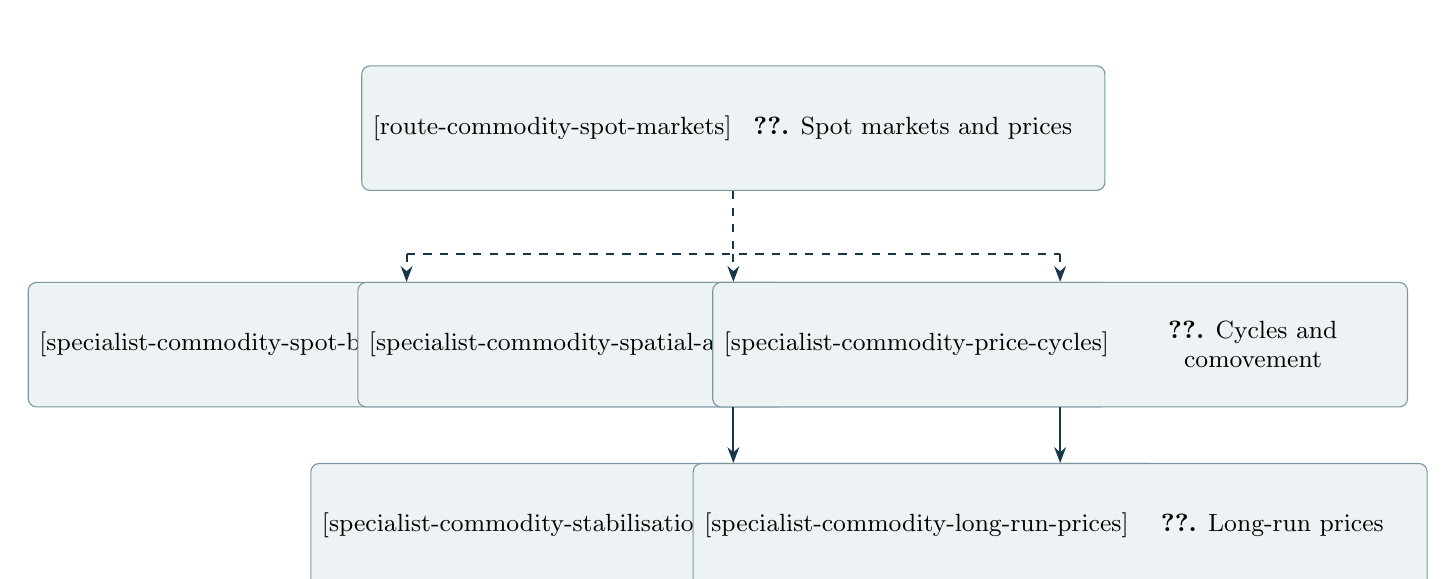
\begin{tikzpicture}[x=1cm,y=1cm]
\node[pathnode] (commodity-spot-markets) at (4.15,0) {\MeasurePathNode{4.6cm}{\textbf{\ref*{route-commodity-spot-markets}.} Spot markets and prices}\hyperref[route-commodity-spot-markets]{\parbox[c][\pathnodeheight][c]{4.6cm}{\centering \textbf{\ref*{route-commodity-spot-markets}.} Spot markets and prices}}};
\node[pathnode] (commodity-spot-benchmarks) at (0.00,-2.75) {\MeasurePathNode{3.65cm}{\textbf{\ref*{specialist-commodity-spot-benchmarks}.} Spot benchmarks}\hyperref[specialist-commodity-spot-benchmarks]{\parbox[c][\pathnodeheight][c]{3.65cm}{\centering \textbf{\ref*{specialist-commodity-spot-benchmarks}.} Spot benchmarks}}};
\node[pathnode] (commodity-spatial-arbitrage) at (4.15,-2.75) {\MeasurePathNode{3.65cm}{\textbf{\ref*{specialist-commodity-spatial-arbitrage}.} Spatial arbitrage}\hyperref[specialist-commodity-spatial-arbitrage]{\parbox[c][\pathnodeheight][c]{3.65cm}{\centering \textbf{\ref*{specialist-commodity-spatial-arbitrage}.} Spatial arbitrage}}};
\node[pathnode] (commodity-price-cycles) at (8.30,-2.75) {\MeasurePathNode{3.65cm}{\textbf{\ref*{specialist-commodity-price-cycles}.} Cycles and comovement}\hyperref[specialist-commodity-price-cycles]{\parbox[c][\pathnodeheight][c]{3.65cm}{\centering \textbf{\ref*{specialist-commodity-price-cycles}.} Cycles and comovement}}};
\node[pathnode] (commodity-stabilisation-trade-policy) at (4.15,-5.05) {\MeasurePathNode{3.65cm}{\textbf{\ref*{specialist-commodity-stabilisation-trade-policy}.} Stocks and trade policy}\hyperref[specialist-commodity-stabilisation-trade-policy]{\parbox[c][\pathnodeheight][c]{3.65cm}{\centering \textbf{\ref*{specialist-commodity-stabilisation-trade-policy}.} Stocks and trade policy}}};
\node[pathnode] (commodity-long-run-prices) at (8.30,-5.05) {\MeasurePathNode{3.65cm}{\textbf{\ref*{specialist-commodity-long-run-prices}.} Long-run prices}\hyperref[specialist-commodity-long-run-prices]{\parbox[c][\pathnodeheight][c]{3.65cm}{\centering \textbf{\ref*{specialist-commodity-long-run-prices}.} Long-run prices}}};
\draw[entryline] (commodity-spot-markets.south) -- (4.15,-1.60);
\draw[entryline] (0.00,-1.60) -- (8.30,-1.60);
\draw[entryarrow] (0.00,-1.60) -- (commodity-spot-benchmarks.north);
\draw[entryarrow] (4.15,-1.60) -- (commodity-spatial-arbitrage.north);
\draw[entryarrow] (8.30,-1.60) -- (commodity-price-cycles.north);
\draw[patharrow] (commodity-spatial-arbitrage.south) -- (commodity-stabilisation-trade-policy.north);
\draw[patharrow] (commodity-price-cycles.south) -- (commodity-long-run-prices.north);
\end{tikzpicture}\end{center}
\textbf{Overview checkpoint.} A section capstone: complete it after \hyperref[specialist-commodity-spot-benchmarks]{\ref*{specialist-commodity-spot-benchmarks}}, \hyperref[specialist-commodity-price-cycles]{\ref*{specialist-commodity-price-cycles}} and \hyperref[specialist-commodity-long-run-prices]{\ref*{specialist-commodity-long-run-prices}}.

\textbf{Bring these foundations with you.}\begin{itemize}
\item \hyperref[specialist-commodity-storage-curves]{Theory of storage, convenience yield and inventories} --- needed by \hyperref[specialist-commodity-spatial-arbitrage]{Spatial arbitrage}.
\item \hyperref[specialist-time-series-volatility]{Time-series econometrics and volatility forecasting} --- needed by \hyperref[specialist-commodity-price-cycles]{Cycles and comovement}.
\end{itemize}\hyperref[learning-map]{Return to the whole-guide DAG.}
\Needspace{12\baselineskip}
\subsection{Spot price assessment and benchmarks: price reporting agencies, auctions and contract pricing}\label{specialist-commodity-spot-benchmarks}
\textbf{Specialist pathway.} In \hyperref[route-commodity-spot-markets]{Commodity spot markets: price formation, market integration and long-run prices}.

\textbf{Outcome.} Read how a spot benchmark is produced---assessment window, data hierarchy, minimum volumes, judgement, or auction rounds---judge how representative and manipulable it is, and decide when a contract should reference a price assessment, an exchange settlement or a negotiated term price.

\textbf{Prerequisites.} Commodity spot markets overview; futures pricing and the basis from Section 20; dealer and search models from Market microstructure and market making help with the theory readings.

\textbf{Review first.} \hyperref[route-commodity-spot-markets]{Commodity spot markets: price formation, market integration and long-run prices}.

\textbf{Required readings, in order}
\begin{enumerate}\raggedright
\Needspace{5\baselineskip}\item \href{institutional_quantitative_finance_reading_list.pdf\#sp-imsirovic-2021}{Adi Imsirovic, \emph{Trading and Price Discovery for Crude Oils: Growth and Development of International Oil Markets}}\CataloguePage{375}\NoteKey{sp-imsirovic-2021}\par\emph{Selection:} The introduction and the chapters on the Brent, Dubai and Oman, and WTI benchmarks.\par \textbf{Mechanics.} Follow how Brent, Dubai--Oman and WTI became the benchmarks that price most traded crude, and who makes and who takes those prices.
\Needspace{5\baselineskip}\item \href{institutional_quantitative_finance_reading_list.pdf\#ec-iosco-pra-2012}{Board of the International Organization of Securities Commissions (IOSCO), Principles for Oil Price Reporting Agencies: Final Report (FR06/12)}\CataloguePage{346}\NoteKey{ec-iosco-pra-2012}\par \textbf{Regulation.} Apply IOSCO's principles on methodology, minimum data, judgement and conflicts of interest to a price reporting agency.
\Needspace{5\baselineskip}\item \href{institutional_quantitative_finance_reading_list.pdf\#sp-iosco-pra-review-2015}{Board of the International Organization of Securities Commissions (IOSCO), Implementation of the Principles for Oil Price Reporting Agencies: Report (FR22/2015)}\CataloguePage{375}\NoteKey{sp-iosco-pra-review-2015}\par \textbf{Regulation.} Check how the four main agencies implemented the principles and what physical-market participants said about assessment quality.
\Needspace{5\baselineskip}\item \href{institutional_quantitative_finance_reading_list.pdf\#sp-oecd-igf-2024}{Jaqueline Taquiri, Thomas Lassourd and Andrew Viola (OECD and Intergovernmental Forum on Mining, Minerals, Metals and Sustainable Development), ``Determining the Price of Minerals: A Transfer Pricing Framework for Lithium''}\CataloguePage{377}\NoteKey{sp-oecd-igf-2024}\par \textbf{Data.} Price an opaque mineral from agency assessments: spot versus contract prices, incoterms and quotation periods, with lithium as the case.
\Needspace{5\baselineskip}\item \href{institutional_quantitative_finance_reading_list.pdf\#sp-duffie-dworczak-2021}{Darrell Duffie and Piotr Dworczak, ``Robust Benchmark Design''}\CataloguePage{376}\NoteKey{sp-duffie-dworczak-2021}\par \textbf{Theory.} Design a fixing from manipulable transactions and see when volume weighting is robust to collusion.
\Needspace{5\baselineskip}\item \href{institutional_quantitative_finance_reading_list.pdf\#sp-duffie-dworczak-zhu-2017}{Darrell Duffie, Piotr Dworczak and Haoxiang Zhu, ``Benchmarks in Search Markets''}\CataloguePage{376}\NoteKey{sp-duffie-dworczak-zhu-2017}\par \textbf{Theory.} See why a published benchmark raises participation and cuts search costs in a bilateral market even though dealer margins fall.
\Needspace{5\baselineskip}\item \href{institutional_quantitative_finance_reading_list.pdf\#sp-iba-lbma-2024}{ICE Benchmark Administration (IBA), LBMA Gold and Silver Prices: Questionnaire for Usage Licence Holders---Feedback Statement}\CataloguePage{376}\NoteKey{sp-iba-lbma-2024}\par \textbf{Mechanics.} Follow the LBMA Gold and Silver Price auctions: rounds, imbalance thresholds, participants and publication.
\Needspace{5\baselineskip}\item \href{institutional_quantitative_finance_reading_list.pdf\#sp-caminschi-heaney-2014}{Andrew Caminschi and Richard Heaney, ``Fixing a Leaky Fixing: Short-Term Market Reactions to the London PM Gold Price Fixing''}\CataloguePage{376}\NoteKey{sp-caminschi-heaney-2014}\par \textbf{Evidence.} Measure information leakage from the old London gold fixing into futures and ETF prices.
\Needspace{5\baselineskip}\item \href{institutional_quantitative_finance_reading_list.pdf\#sp-hauptfleisch-2016}{Martin Hauptfleisch, Tālis J. Putniņš and Brian Lucey, ``Who Sets the Price of Gold? London or New York''}\CataloguePage{376}\NoteKey{sp-hauptfleisch-2016}\par \textbf{Evidence.} Find whether London spot or New York futures set the gold price, and why market structure decides.
\Needspace{5\baselineskip}\item \href{institutional_quantitative_finance_reading_list.pdf\#sp-warell-2014}{Linda Wårell, ``The Effect of a Change in Pricing Regime on Iron Ore Prices''}\CataloguePage{376}\NoteKey{sp-warell-2014}\par \textbf{Evidence.} Test whether iron ore's move from annual benchmark contracts to spot-linked pricing raised volatility or prices.
\Needspace{5\baselineskip}\item \href{institutional_quantitative_finance_reading_list.pdf\#sp-hubbard-weiner-1991}{R. Glenn Hubbard and Robert J. Weiner, ``Efficient Contracting and Market Power: Evidence from the U.S. Natural Gas Industry''}\CataloguePage{377}\NoteKey{sp-hubbard-weiner-1991}\par \textbf{Evidence.} See how long-term contracts set initial prices and escalator clauses when bilateral bargaining replaces a spot market.
\end{enumerate}
\Needspace{5\baselineskip}\textbf{Checkpoint.} Take one price assessment that settles a futures or swap contract: Dated Brent, a lithium CIF Asia assessment or the LBMA Gold Price. From the published methodology, write down its assessment window, data hierarchy, minimum-volume rule and use of judgement, and compare it with the nearest exchange price over one month. Simulate how one participant's trades inside the window would move a volume-weighted fixing and a trimmed median, and state whether a buyer should sign a term contract at the assessment, at a futures settlement or at a fixed price with an escalator.

\textbf{Optional branches.} \href{institutional_quantitative_finance_reading_list.pdf\#sp-ma-2013}{Model how iron ore spot volatility changed with the forward pricing mechanism.}\BranchPage{376} \href{institutional_quantitative_finance_reading_list.pdf\#dm-barzykin-bergault-gueant-metals}{Quote spot precious metals as a dealer whose hedge is in futures.}\BranchPage{173} \href{institutional_quantitative_finance_reading_list.pdf\#wide-evans-wmr-fix}{Compare a commodity fixing with trading around the London 4pm FX fix.}\BranchPage{289} \href{institutional_quantitative_finance_reading_list.pdf\#w3-brugler-benchmarking-benchmarks}{Separate information from noise in a benchmark with a state-space model.}\BranchPage{110}
\par{\small \hyperref[learning-map]{Learning pathway DAG} \textbar{} \hyperref[route-commodity-spot-markets]{Section overview} \textbar{} \hyperref[map-commodity-spot-markets]{Section DAG}\NoteKey{commodity-spot-benchmarks}}
\Needspace{12\baselineskip}
\subsection{Spatial arbitrage and market integration: transport costs, pipelines and information}\label{specialist-commodity-spatial-arbitrage}
\textbf{Specialist pathway.} In \hyperref[route-commodity-spot-markets]{Commodity spot markets: price formation, market integration and long-run prices}.

\textbf{Outcome.} Test whether two spot markets are integrated once transfer costs are measured, explain location differentials from pipeline, shipping and sanctions constraints, and measure how information frictions widen price dispersion.

\textbf{Prerequisites.} Commodity spot markets overview; theory of storage, convenience yield and inventories (20.1); cointegration and threshold time-series models.

\textbf{Review first.} \hyperref[route-commodity-spot-markets]{Commodity spot markets: price formation, market integration and long-run prices}; \hyperref[specialist-commodity-storage-curves]{Theory of storage, convenience yield and inventories}.

\textbf{Required readings, in order}
\begin{enumerate}\raggedright
\Needspace{5\baselineskip}\item \href{institutional_quantitative_finance_reading_list.pdf\#sp-fackler-goodwin-2001}{Paul L. Fackler and Barry K. Goodwin, ``Spatial Price Analysis''}\CataloguePage{377}\NoteKey{sp-fackler-goodwin-2001}\par \textbf{Foundations.} Set out the spatial arbitrage condition and the main tests of market integration.
\Needspace{5\baselineskip}\item \href{institutional_quantitative_finance_reading_list.pdf\#sp-baulch-1997}{Bob Baulch, ``Transfer Costs, Spatial Arbitrage, and Testing for Food Market Integration''}\CataloguePage{377}\NoteKey{sp-baulch-1997}\par \textbf{Methods.} Use transfer-cost data in a parity-bounds model instead of price correlations.
\Needspace{5\baselineskip}\item \href{institutional_quantitative_finance_reading_list.pdf\#sp-barrett-li-2002}{Christopher B. Barrett and Jau Rong Li, ``Distinguishing between Equilibrium and Integration in Spatial Price Analysis''}\CataloguePage{377}\NoteKey{sp-barrett-li-2002}\par \textbf{Methods.} Separate market integration from competitive equilibrium with price, cost and trade-flow data.
\Needspace{5\baselineskip}\item \href{institutional_quantitative_finance_reading_list.pdf\#cf-coleman-2009}{Andrew Coleman, ``Storage, Slow Transport, and the Law of One Price: Theory with Evidence from Nineteenth-Century U.S. Corn Markets''}\CataloguePage{377}\NoteKey{cf-coleman-2009}\par \textbf{Theory.} Add slow transport to storage: regional stock-outs and local price spikes in a competitive market.
\Needspace{5\baselineskip}\item \href{institutional_quantitative_finance_reading_list.pdf\#sp-jacks-orourke-williamson-2011}{David S. Jacks, Kevin H. O'Rourke and Jeffrey G. Williamson, ``Commodity Price Volatility and World Market Integration since 1700''}\CataloguePage{378}\NoteKey{sp-jacks-orourke-williamson-2011}\par \textbf{Evidence.} Relate world market integration to commodity price volatility over three centuries.
\Needspace{5\baselineskip}\item \href{institutional_quantitative_finance_reading_list.pdf\#sp-jensen-2007}{Robert Jensen, ``The Digital Provide: Information (Technology), Market Performance, and Welfare in the South Indian Fisheries Sector''}\CataloguePage{378}\NoteKey{sp-jensen-2007}\par \textbf{Evidence.} See mobile phones bring Kerala fish markets close to the law of one price.
\Needspace{5\baselineskip}\item \href{institutional_quantitative_finance_reading_list.pdf\#sp-allen-2014}{Treb Allen, ``Information Frictions in Trade''}\CataloguePage{378}\NoteKey{sp-allen-2014}\par \textbf{Evidence.} Estimate how much regional price dispersion comes from costly search for prices.
\Needspace{5\baselineskip}\item \href{institutional_quantitative_finance_reading_list.pdf\#sp-steinwender-2018}{Claudia Steinwender, ``Real Effects of Information Frictions: When the States and the Kingdom Became United''}\CataloguePage{378}\NoteKey{sp-steinwender-2018}\par \textbf{Evidence.} Measure how the transatlantic telegraph narrowed and steadied the cotton price gap.
\Needspace{5\baselineskip}\item \href{institutional_quantitative_finance_reading_list.pdf\#sp-borenstein-kellogg-2014}{Severin Borenstein and Ryan Kellogg, ``The Incidence of an Oil Glut: Who Benefits from Cheap Crude Oil in the Midwest?''}\CataloguePage{378}\NoteKey{sp-borenstein-kellogg-2014}\par \textbf{Evidence.} Follow a landlocked crude glut: discounted WTI did not pass through to Midwest fuel prices.
\Needspace{5\baselineskip}\item \href{institutional_quantitative_finance_reading_list.pdf\#sp-agerton-upton-2019}{Mark Agerton and Gregory B. Upton, ``Decomposing Crude Price Differentials: Domestic Shipping Constraints or the Crude Oil Export Ban?''}\CataloguePage{378}\NoteKey{sp-agerton-upton-2019}\par \textbf{Evidence.} Split the WTI discount into pipeline constraints and the crude export ban.
\Needspace{5\baselineskip}\item \href{institutional_quantitative_finance_reading_list.pdf\#sp-oliver-mason-finnoff-2014}{Matthew E. Oliver, Charles F. Mason and David Finnoff, ``Pipeline Congestion and Basis Differentials''}\CataloguePage{379}\NoteKey{sp-oliver-mason-finnoff-2014}\par \textbf{Evidence.} Price pipeline congestion into natural gas basis differentials, and see storage dampen it.
\Needspace{5\baselineskip}\item \href{institutional_quantitative_finance_reading_list.pdf\#sp-kilian-rapson-schipper-2026}{Lutz Kilian, David Rapson and Burkhard Schipper, ``The Impact of the 2022 Oil Embargo and Price Cap on Russian Oil Prices''}\CataloguePage{379}\NoteKey{sp-kilian-rapson-schipper-2026}\par \textbf{Evidence.} Split the post-2022 Urals discount into longer shipping routes and buyer bargaining power.
\end{enumerate}
\Needspace{5\baselineskip}\textbf{Checkpoint.} For two locations of one commodity---WTI at Cushing and Houston, Henry Hub and a western gas hub, or two grain terminals---collect daily spot prices and a transfer-cost series (pipeline tariff, freight or barge rate). Classify days by whether the spread lies inside, at or outside the transfer-cost band, fit a parity-bounds or threshold error-correction model, and relate the episodes outside the band to capacity outages, sanctions or information events.

\textbf{Optional branches.} \href{institutional_quantitative_finance_reading_list.pdf\#sp-aker-2010}{Compare grain price dispersion in Niger before and after mobile phones.}\BranchPage{378} \href{institutional_quantitative_finance_reading_list.pdf\#cf-brancaccio-2020}{Make transport costs endogenous with a model of the ocean shipping market.}\BranchPage{387}
\par{\small \hyperref[learning-map]{Learning pathway DAG} \textbar{} \hyperref[route-commodity-spot-markets]{Section overview} \textbar{} \hyperref[map-commodity-spot-markets]{Section DAG}\NoteKey{commodity-spatial-arbitrage}}
\Needspace{12\baselineskip}
\subsection{Commodity price cycles, comovement and macro drivers}\label{specialist-commodity-price-cycles}
\textbf{Specialist pathway.} In \hyperref[route-commodity-spot-markets]{Commodity spot markets: price formation, market integration and long-run prices}.

\textbf{Outcome.} Date commodity booms and slumps, extract the common factor in commodity prices and tie it to global activity, real interest rates and the dollar, and judge which predictors forecast spot prices out of sample.

\textbf{Prerequisites.} Commodity spot markets overview; time-series econometrics (VARs, dynamic factor models, structural identification). Oil supply and demand shocks (24.1) applies the same tools to crude oil.

\textbf{Review first.} \hyperref[route-commodity-spot-markets]{Commodity spot markets: price formation, market integration and long-run prices}; \hyperref[specialist-time-series-volatility]{Time-series econometrics and volatility forecasting}.

\textbf{Required readings, in order}
\begin{enumerate}\raggedright
\Needspace{5\baselineskip}\item \href{institutional_quantitative_finance_reading_list.pdf\#sp-cashin-mcdermott-scott-2002}{Paul Cashin, C. John McDermott and Alasdair Scott, ``Booms and Slumps in World Commodity Prices''}\CataloguePage{379}\NoteKey{sp-cashin-mcdermott-scott-2002}\par \textbf{Evidence.} Date booms and slumps: slumps last longer than booms and neither ends predictably.
\Needspace{5\baselineskip}\item \href{institutional_quantitative_finance_reading_list.pdf\#sp-pindyck-rotemberg-1990}{Robert S. Pindyck and Julio J. Rotemberg, ``The Excess Co-Movement of Commodity Prices''}\CataloguePage{380}\NoteKey{sp-pindyck-rotemberg-1990}\par \textbf{Evidence.} Test whether unrelated commodity prices move together more than macro fundamentals explain.
\Needspace{5\baselineskip}\item \href{institutional_quantitative_finance_reading_list.pdf\#sp-byrne-fazio-fiess-2013}{Joseph P. Byrne, Giorgio Fazio and Norbert Fiess, ``Primary Commodity Prices: Co-movements, Common Factors and Fundamentals''}\CataloguePage{380}\NoteKey{sp-byrne-fazio-fiess-2013}\par \textbf{Evidence.} Estimate a common factor in commodity prices and relate it to real interest rates and uncertainty.
\Needspace{5\baselineskip}\item \href{institutional_quantitative_finance_reading_list.pdf\#sp-delle-chiaie-2022}{Simona Delle Chiaie, Laurent Ferrara and Domenico Giannone, ``Common Factors of Commodity Prices''}\CataloguePage{380}\NoteKey{sp-delle-chiaie-2022}\par \textbf{Methods.} Split commodity prices into global, block and idiosyncratic factors.
\Needspace{5\baselineskip}\item \href{institutional_quantitative_finance_reading_list.pdf\#sp-alquist-bhattarai-coibion-2020}{Ron Alquist, Saroj Bhattarai and Olivier Coibion, ``Commodity-Price Comovement and Global Economic Activity''}\CataloguePage{380}\NoteKey{sp-alquist-bhattarai-coibion-2020}\par \textbf{Theory.} Give the common factors a structural reading from a general-equilibrium model of commodity prices.
\Needspace{5\baselineskip}\item \href{institutional_quantitative_finance_reading_list.pdf\#ec-kilian-zhou-2018}{Lutz Kilian and Xiaoqing Zhou, ``Modeling Fluctuations in the Global Demand for Commodities''}\CataloguePage{348}\NoteKey{ec-kilian-zhou-2018}\par \textbf{Data.} Choose a measure of global real activity suited to industrial commodity prices.
\Needspace{5\baselineskip}\item \href{institutional_quantitative_finance_reading_list.pdf\#sp-frankel-2008}{Jeffrey A. Frankel, ``The Effect of Monetary Policy on Real Commodity Prices''}\CataloguePage{380}\NoteKey{sp-frankel-2008}\par \textbf{Theory.} Connect real interest rates to real commodity prices.
\Needspace{5\baselineskip}\item \href{institutional_quantitative_finance_reading_list.pdf\#sp-akram-2009}{Q. Farooq Akram, ``Commodity Prices, Interest Rates and the Dollar''}\CataloguePage{381}\NoteKey{sp-akram-2009}\par \textbf{Evidence.} Estimate how real interest rates and the dollar move oil, metals and food prices.
\Needspace{5\baselineskip}\item \href{institutional_quantitative_finance_reading_list.pdf\#sp-fsu-2017}{Andrés Fernández, Stephanie Schmitt-Grohé and Martín Uribe, ``World Shocks, World Prices, and Business Cycles: An Empirical Investigation''}\CataloguePage{381}\NoteKey{sp-fsu-2017}\par \textbf{Evidence.} Measure how much output volatility commodity prices transmit across 138 economies.
\Needspace{5\baselineskip}\item \href{institutional_quantitative_finance_reading_list.pdf\#sp-chinn-coibion-2014}{Menzie D. Chinn and Olivier Coibion, ``The Predictive Content of Commodity Futures''}\CataloguePage{381}\NoteKey{sp-chinn-coibion-2014}\par \textbf{Validation.} Check how well futures prices forecast spot prices across commodity groups.
\Needspace{5\baselineskip}\item \href{institutional_quantitative_finance_reading_list.pdf\#sp-gargano-timmermann-2014}{Antonio Gargano and Allan Timmermann, ``Forecasting Commodity Price Indexes Using Macroeconomic and Financial Predictors''}\CataloguePage{381}\NoteKey{sp-gargano-timmermann-2014}\par \textbf{Validation.} Forecast commodity spot indexes out of sample with macro and financial predictors, by state of the economy.
\end{enumerate}
\Needspace{5\baselineskip}\textbf{Checkpoint.} Assemble monthly real prices for at least 30 commodities since 1970. Date booms and slumps with a turning-point rule, extract a global factor with a dynamic factor model, and relate it to a global activity index, the real interest rate and the trade-weighted dollar. Then forecast the index twelve months ahead with futures, commodity currencies and macro predictors, and compare the errors with a no-change forecast in expansions and recessions.

\textbf{Optional branches.} \href{institutional_quantitative_finance_reading_list.pdf\#sp-deb-trivedi-varangis-1996}{Re-test excess comovement with GARCH models: the evidence weakens.}\BranchPage{380} \href{institutional_quantitative_finance_reading_list.pdf\#sp-baffes-kabundi-2023}{Split commodity prices into transitory and permanent shocks with a band-pass filter.}\BranchPage{381} \href{institutional_quantitative_finance_reading_list.pdf\#sp-frankel-2014}{Add expectations and risk to the interest-rate channel in a carry-trade model.}\BranchPage{380} \href{institutional_quantitative_finance_reading_list.pdf\#sp-chen-rogoff-2003}{See commodity prices drive the real exchange rates of commodity exporters.}\BranchPage{381} \href{institutional_quantitative_finance_reading_list.pdf\#ec-chen-rogoff-rossi-2010}{Forecast commodity prices with commodity currencies.}\BranchPage{348}
\par{\small \hyperref[learning-map]{Learning pathway DAG} \textbar{} \hyperref[route-commodity-spot-markets]{Section overview} \textbar{} \hyperref[map-commodity-spot-markets]{Section DAG}\NoteKey{commodity-price-cycles}}
\Needspace{12\baselineskip}
\subsection{Price stabilisation, public stocks and export restrictions}\label{specialist-commodity-stabilisation-trade-policy}
\textbf{Specialist pathway.} In \hyperref[route-commodity-spot-markets]{Commodity spot markets: price formation, market integration and long-run prices}.

\textbf{Outcome.} Evaluate buffer stocks, price bands, strategic reserves and export controls with the storage model, estimate how much a stock release or an export ban moves world spot prices, and explain why unilateral insulation amplifies world price spikes.

\textbf{Prerequisites.} Spatial arbitrage and market integration (21.2); the competitive storage model from the theory of storage (20.1).

\textbf{Review first.} \hyperref[specialist-commodity-spatial-arbitrage]{Spatial arbitrage and market integration: transport costs, pipelines and information}.

\textbf{Required readings, in order}
\begin{enumerate}\raggedright
\Needspace{5\baselineskip}\item \href{institutional_quantitative_finance_reading_list.pdf\#sp-gouel-wright-2026}{Christophe Gouel and Brian D. Wright, ``Storage and the Economics of Commodity Price Stabilization''}\CataloguePage{383}\NoteKey{sp-gouel-wright-2026}\par \textbf{Theory.} Weigh price bands, storage subsidies and export controls against private storage in the rational-expectations storage model.
\Needspace{5\baselineskip}\item \href{institutional_quantitative_finance_reading_list.pdf\#sp-gouel-2012}{Christophe Gouel, ``Agricultural Price Instability: A Survey of Competing Explanations and Remedies''}\CataloguePage{383}\NoteKey{sp-gouel-2012}\par \textbf{Theory.} Separate cobweb and rational-expectations explanations of agricultural price instability and their policy remedies.
\Needspace{5\baselineskip}\item \href{institutional_quantitative_finance_reading_list.pdf\#sp-wright-williams-1982}{Brian D. Wright and Jeffrey C. Williams, ``The Roles of Public and Private Storage in Managing Oil Import Disruptions''}\CataloguePage{383}\NoteKey{sp-wright-williams-1982}\par \textbf{Theory.} Size public oil stocks when private storage responds and a price ceiling may be imposed.
\Needspace{5\baselineskip}\item \href{institutional_quantitative_finance_reading_list.pdf\#sp-kilian-zhou-2020}{Lutz Kilian and Xiaoqing Zhou, ``Does Drawing Down the US Strategic Petroleum Reserve Help Stabilize Oil Prices?''}\CataloguePage{383}\NoteKey{sp-kilian-zhou-2020}\par \textbf{Evidence.} Estimate what SPR drawdowns and exchanges have done to the real oil price.
\Needspace{5\baselineskip}\item \href{institutional_quantitative_finance_reading_list.pdf\#sp-iea-2026}{International Energy Agency, IEA Member Countries to Carry Out Largest Ever Oil Stock Release amid Market Disruptions from Middle East Conflict}\CataloguePage{384}\NoteKey{sp-iea-2026}\par \textbf{Implementation.} Read the scale and trigger of the IEA's largest coordinated stock release.
\Needspace{5\baselineskip}\item \href{institutional_quantitative_finance_reading_list.pdf\#sp-gilbert-2010}{Christopher L. Gilbert, ``How to Understand High Food Prices''}\CataloguePage{384}\NoteKey{sp-gilbert-2010}\par \textbf{Evidence.} Attribute the 2007--08 food price rise to common macro and monetary factors rather than crop-specific shocks.
\Needspace{5\baselineskip}\item \href{institutional_quantitative_finance_reading_list.pdf\#sp-headey-2011}{Derek Headey, ``Rethinking the Global Food Crisis: The Role of Trade Shocks''}\CataloguePage{384}\NoteKey{sp-headey-2011}\par \textbf{Evidence.} Trace the 2008 rice and grain price overshoot to export surges and restrictions.
\Needspace{5\baselineskip}\item \href{institutional_quantitative_finance_reading_list.pdf\#sp-martin-anderson-2012}{Will Martin and Kym Anderson, ``Export Restrictions and Price Insulation During Commodity Price Booms''}\CataloguePage{384}\NoteKey{sp-martin-anderson-2012}\par \textbf{Evidence.} Measure how much insulating trade policy added to the rice and wheat spikes.
\Needspace{5\baselineskip}\item \href{institutional_quantitative_finance_reading_list.pdf\#sp-giordani-rocha-ruta-2016}{Paolo E. Giordani, Nadia Rocha and Michele Ruta, ``Food Prices and the Multiplier Effect of Trade Policy''}\CataloguePage{384}\NoteKey{sp-giordani-rocha-ruta-2016}\par \textbf{Evidence.} See export restrictions and import liberalisation feed on each other as a multiplier.
\Needspace{5\baselineskip}\item \href{institutional_quantitative_finance_reading_list.pdf\#sp-gotz-2013}{Linde Götz, Thomas Glauben and Bernhard Brümmer, ``Wheat Export Restrictions and Domestic Market Effects in Russia and Ukraine during the Food Crisis''}\CataloguePage{384}\NoteKey{sp-gotz-2013}\par \textbf{Evidence.} Measure how Russia's and Ukraine's wheat export controls cut domestic prices off from world markets.
\end{enumerate}
\Needspace{5\baselineskip}\textbf{Checkpoint.} Simulate a competitive storage model for one grain with a public stock that defends a price band, and compare price variance, average stocks and fiscal cost with a storage-subsidy rule. Then take the 2008 rice or 2022 wheat episode: list export restrictions by date and share of world trade, estimate the world price response with Martin and Anderson's insulation calculation, and set the 2026 IEA stock release against Kilian and Zhou's estimates of what earlier releases did to the oil price.

\textbf{Optional branches.} \href{institutional_quantitative_finance_reading_list.pdf\#sp-gilbert-1996}{Review why the international commodity agreements' buffer stocks and quotas failed.}\BranchPage{385} \href{institutional_quantitative_finance_reading_list.pdf\#sp-gouel-jean-2015}{Design optimal storage and trade policy for a small open food importer.}\BranchPage{385} \href{institutional_quantitative_finance_reading_list.pdf\#sp-glauber-2023}{Follow the export restrictions imposed after the 2022 invasion of Ukraine.}\BranchPage{385}
\par{\small \hyperref[learning-map]{Learning pathway DAG} \textbar{} \hyperref[route-commodity-spot-markets]{Section overview} \textbar{} \hyperref[map-commodity-spot-markets]{Section DAG}\NoteKey{commodity-stabilisation-trade-policy}}
\Needspace{12\baselineskip}
\subsection{Long-run commodity prices: exhaustibility, secular trends and supercycles}\label{specialist-commodity-long-run-prices}
\textbf{Specialist pathway.} In \hyperref[route-commodity-spot-markets]{Commodity spot markets: price formation, market integration and long-run prices}.

\textbf{Outcome.} Test the Hotelling rule and the Prebisch--Singer hypothesis on long price series, separate secular trends from supercycles and boom--bust episodes, and judge what supply responses imply for long-dated price assumptions.

\textbf{Prerequisites.} Commodity price cycles, comovement and macro drivers (21.3); unit-root and trend tests and band-pass filters.

\textbf{Review first.} \hyperref[specialist-commodity-price-cycles]{Commodity price cycles, comovement and macro drivers}.

\textbf{Required readings, in order}
\begin{enumerate}\raggedright
\Needspace{5\baselineskip}\item \href{institutional_quantitative_finance_reading_list.pdf\#w5-hotelling}{Harold Hotelling, ``The Economics of Exhaustible Resources''}\CataloguePage{427}\NoteKey{w5-hotelling}\par \textbf{Theory.} Start from the Hotelling rule: scarcity rents rise at the rate of interest under competitive extraction.
\Needspace{5\baselineskip}\item \href{institutional_quantitative_finance_reading_list.pdf\#sp-slade-thille-2009}{Margaret E. Slade and Henry Thille, ``Whither Hotelling: Tests of the Theory of Exhaustible Resources''}\CataloguePage{381}\NoteKey{sp-slade-thille-2009}\par \textbf{Evidence.} Review descriptive and structural tests of Hotelling and their econometric pitfalls.
\Needspace{5\baselineskip}\item \href{institutional_quantitative_finance_reading_list.pdf\#w5-anderson-kellogg-salant}{Soren T. Anderson, Ryan Kellogg and Stephen W. Salant, ``Hotelling under Pressure''}\CataloguePage{427}\NoteKey{w5-anderson-kellogg-salant}\par \textbf{Evidence.} Recast Hotelling around the drilling decision: output from existing wells ignores price.
\Needspace{5\baselineskip}\item \href{institutional_quantitative_finance_reading_list.pdf\#sp-newell-prest-2019}{Richard G. Newell and Brian C. Prest, ``The Unconventional Oil Supply Boom: Aggregate Price Response from Microdata''}\CataloguePage{383}\NoteKey{sp-newell-prest-2019}\par \textbf{Evidence.} Measure how fast shale supply responds to price and why it is not a 90-day swing producer.
\Needspace{5\baselineskip}\item \href{institutional_quantitative_finance_reading_list.pdf\#sp-pindyck-1999}{Robert S. Pindyck, ``The Long-Run Evolution of Energy Prices''}\CataloguePage{382}\NoteKey{sp-pindyck-1999}\par \textbf{Methods.} Model 127 years of energy prices and ask what fluctuating trends imply for 20-year forecasts.
\Needspace{5\baselineskip}\item \href{institutional_quantitative_finance_reading_list.pdf\#sp-grilli-yang-1988}{Enzo R. Grilli and Maw Cheng Yang, ``Primary Commodity Prices, Manufactured Goods Prices, and the Terms of Trade of Developing Countries: What the Long Run Shows''}\CataloguePage{382}\NoteKey{sp-grilli-yang-1988}\par \textbf{Evidence.} Measure the secular decline in commodity prices relative to manufactures since 1900.
\Needspace{5\baselineskip}\item \href{institutional_quantitative_finance_reading_list.pdf\#sp-cashin-mcdermott-2002}{Paul Cashin and C. John McDermott, ``The Long-Run Behavior of Commodity Prices: Small Trends and Big Variability''}\CataloguePage{382}\NoteKey{sp-cashin-mcdermott-2002}\par \textbf{Evidence.} Weigh a small downward trend against large and rising variability.
\Needspace{5\baselineskip}\item \href{institutional_quantitative_finance_reading_list.pdf\#sp-harvey-2010}{David I. Harvey, Neil M. Kellard, Jakob B. Madsen and Mark E. Wohar, ``The Prebisch--Singer Hypothesis: Four Centuries of Evidence''}\CataloguePage{382}\NoteKey{sp-harvey-2010}\par \textbf{Evidence.} Test Prebisch--Singer on four centuries of data with trend tests robust to unit roots.
\Needspace{5\baselineskip}\item \href{institutional_quantitative_finance_reading_list.pdf\#sp-erten-ocampo-2013}{Bilge Erten and José Antonio Ocampo, ``Super Cycles of Commodity Prices since the Mid-Nineteenth Century''}\CataloguePage{382}\NoteKey{sp-erten-ocampo-2013}\par \textbf{Evidence.} Extract 30--40-year super cycles and link them to world GDP.
\Needspace{5\baselineskip}\item \href{institutional_quantitative_finance_reading_list.pdf\#sp-jacks-2019}{David S. Jacks, ``From Boom to Bust: A Typology of Real Commodity Prices in the Long Run''}\CataloguePage{382}\NoteKey{sp-jacks-2019}\par \textbf{Evidence.} Separate long-run trends, medium-run cycles and boom--bust episodes across 40 commodities.
\Needspace{5\baselineskip}\item \href{institutional_quantitative_finance_reading_list.pdf\#sp-stuermer-2018}{Martin Stuermer, ``150 Years of Boom and Bust: What Drives Mineral Commodity Prices?''}\CataloguePage{382}\NoteKey{sp-stuermer-2018}\par \textbf{Evidence.} Identify demand and supply shocks in 175 years of metal prices and production.
\Needspace{5\baselineskip}\item \href{institutional_quantitative_finance_reading_list.pdf\#sp-baffes-kabundi-2024}{John Baffes and Alain Kabundi, ``Do Supercycles Dominate Commodity Price Movements?''}\CataloguePage{383}\NoteKey{sp-baffes-kabundi-2024}\par \textbf{Counter-evidence.} Check how much supercycles contribute to price variability against permanent shocks.
\end{enumerate}
\Needspace{5\baselineskip}\textbf{Checkpoint.} Using a long annual series for one exhaustible resource (copper, oil or coal) and one annual crop, deflated by a manufactures unit-value index, test for a deterministic trend robust to unit roots and extract a 20--70-year supercycle with a band-pass filter. Compare the implied long-run price with the longest-dated futures price and an analyst consensus, and say how much of the resource's price path a Hotelling rent can explain given reserve additions and the observed supply elasticity.

\textbf{Optional branches.} \href{institutional_quantitative_finance_reading_list.pdf\#sp-asker-2019}{Quantify misallocation and market power in global oil extraction.}\BranchPage{383}
\par{\small \hyperref[learning-map]{Learning pathway DAG} \textbar{} \hyperref[route-commodity-spot-markets]{Section overview} \textbar{} \hyperref[map-commodity-spot-markets]{Section DAG}\NoteKey{commodity-long-run-prices}}
\clearpage
\section{Physical commodity markets: delivery, price discovery and trading}\label{route-physical-commodity-markets}
\label{route-29}
\textbf{Learning sequence.} Start with contract design and delivery: metals, agriculture and crude oil build on it. Price discovery and fundamental data, freight, and trading firms and margin stress are separate entry points; freight and trading firms also need hedging (20.3). Risk premia and commodity investing follow in the next section, and oil-price shocks in the one after.

\textbf{Section goals.} Across its pathways, this section teaches you to:
\begin{itemize}[leftmargin=1.4em,itemsep=0pt,topsep=1pt]
\item read delivery terms and recognise convergence failures and manipulation (\hyperref[specialist-futures-delivery-manipulation]{\ref*{specialist-futures-delivery-manipulation}})
\item connect metal forward curves to inventories, delivery and lease economics (\hyperref[specialist-metals-storage-delivery]{\ref*{specialist-metals-storage-delivery}})
\item turn crop supply and use into a deliverable futures exposure (\hyperref[specialist-agricultural-futures-delivery]{\ref*{specialist-agricultural-futures-delivery}})
\item map crude and refined-product exposures to benchmarks and spreads (\hyperref[specialist-crude-oil-products]{\ref*{specialist-crude-oil-products}})
\item locate price discovery and measure reactions to fundamental reports (\hyperref[specialist-commodity-information-discovery]{\ref*{specialist-commodity-information-discovery}})
\item hedge freight with Baltic routes and freight forward agreements (\hyperref[specialist-freight-forward-hedging]{\ref*{specialist-freight-forward-hedging}})
\item follow trading-firm finance and margin stress through clearing and bank funding (\hyperref[specialist-commodity-trading-finance]{\ref*{specialist-commodity-trading-finance}})
\end{itemize}
\textbf{Overview outcome.} Specify a physically delivered contract's delivery terms and show how a delivery-rule change, a fundamental-data surprise and higher initial margin would each alter a calendar-spread hedge of a physical position.

\textbf{Prerequisites.} Commodity futures: storage, curves, hedging and options; commodity spot markets (Section 21) helps for benchmarks and location spreads; exchange microstructure from Execution, trading costs and market structure helps but is not required.

\textbf{Review first.} \hyperref[route-energy-commodities]{Commodity futures: storage, curves, hedging and options}.

\textbf{Required readings, in order}
\begin{enumerate}\raggedright
\Needspace{5\baselineskip}\item \href{institutional_quantitative_finance_reading_list.pdf\#wide-pirrong-trading-firms}{Craig Pirrong, ``The Economics of Commodity Trading Firms''}\CataloguePage{374}\NoteKey{wide-pirrong-trading-firms}\par See how physical traders transform commodities in space, time and form and manage the price and credit risk that futures hedge.
\Needspace{5\baselineskip}\item \href{institutional_quantitative_finance_reading_list.pdf\#cf-carlton-1984}{Dennis W. Carlton, ``Futures Markets: Their Purpose, Their History, Their Growth, Their Successes and Failures''}\CataloguePage{369}\NoteKey{cf-carlton-1984}\par Ask why futures markets exist and why most new contracts fail before studying how delivery rules work.
\Needspace{5\baselineskip}\item \href{institutional_quantitative_finance_reading_list.pdf\#depth-ice-coffee-delivery}{ICE Futures U.S., Coffee ``C'' Futures Rules; USDA Foreign Agricultural Service, Coffee: World Markets and Trade route}\CataloguePage{368}\NoteKey{depth-ice-coffee-delivery}\par\emph{Selection:} ICE Coffee C futures rules; the paired USDA market report supplies optional physical-market context.\par Check how quality and delivery rules create a distinct agricultural basis.
\Needspace{5\baselineskip}\item \href{institutional_quantitative_finance_reading_list.pdf\#wide-lme-nickel-review}{Oliver Wyman (for the London Metal Exchange), ``Independent Review of Events in the Nickel Market in March 2022''}\CataloguePage{539}\NoteKey{wide-lme-nickel-review}\par See how OTC exposure, margin calls and exchange intervention interacted in the March 2022 nickel squeeze before relying on delivery and clearing rules.
\end{enumerate}
\Needspace{5\baselineskip}\textbf{Checkpoint.} Choose one physically delivered commodity contract and specify its delivery instrument, grades, locations, storage or shipping costs, and last trading and notice dates. Show how a delivery-rule change, a surprise in the weekly inventory or monthly crop report, and a doubling of initial margin would each alter a calendar-spread hedge of a physical position.

\textbf{Optional branches.} \href{institutional_quantitative_finance_reading_list.pdf\#section.14.24}{Extend to freight and weather indices when logistics or climate is the binding risk.}\BranchPage{385}
\par\textbf{Continue in this section.} \hyperref[specialist-futures-delivery-manipulation]{Futures contract design, delivery options, convergence and manipulation}; \hyperref[specialist-metals-storage-delivery]{Precious and base metals: storage, lending and delivery}; \hyperref[specialist-agricultural-futures-delivery]{Agricultural futures, crop balance and delivery}; \hyperref[specialist-crude-oil-products]{Crude oil and refined products: benchmarks, spreads and price reporting}; \hyperref[specialist-commodity-information-discovery]{Price discovery and fundamental information: crop and inventory reports, analysts and satellites}; \hyperref[specialist-freight-forward-hedging]{Freight markets, Baltic benchmarks and FFAs}; \hyperref[specialist-commodity-trading-finance]{Commodity trading firms, financing and margin stress}.
\par{\small \hyperref[learning-map]{Learning pathway DAG} \textbar{} \hyperref[map-physical-commodity-markets]{Section DAG}\NoteKey{physical-commodity-markets}}
\clearpage
\subsection*{Physical commodity markets: delivery, price discovery and trading: pathway DAG}\phantomsection\label{map-physical-commodity-markets}
\addcontentsline{toc}{subsection}{Physical commodity markets: delivery, price discovery and trading: pathway DAG}
Start with the section overview's readings, for orientation. Solid arrows show prerequisites within this section. Dashed connectors identify entry points with no further prerequisite in this section; the linked foundations below still apply. Follow the arrows for dependencies and the subsection numbers for reading order. Every node is clickable.
\begin{center}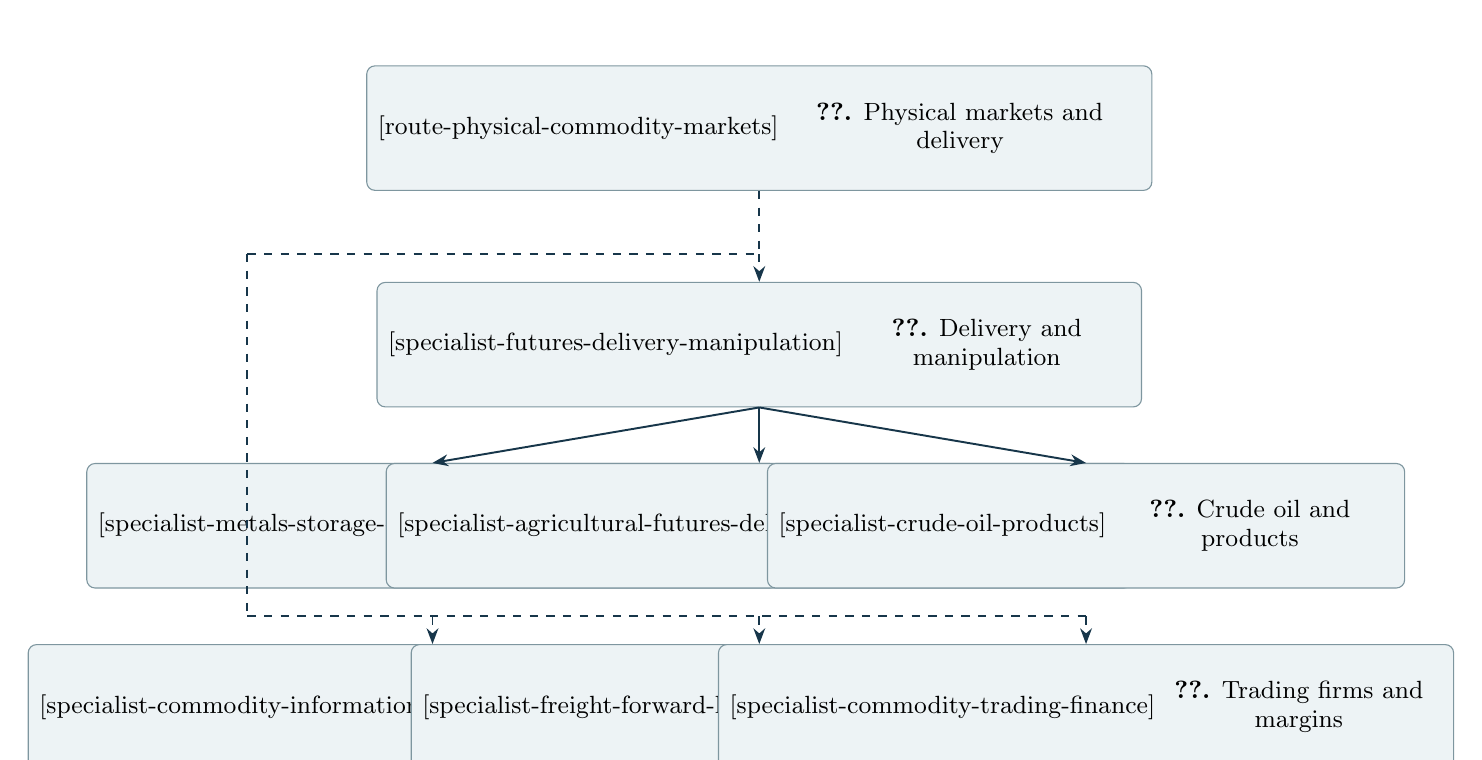
\begin{tikzpicture}[x=1cm,y=1cm]
\node[pathnode] (physical-commodity-markets) at (4.15,0) {\MeasurePathNode{4.6cm}{\textbf{\ref*{route-physical-commodity-markets}.} Physical markets and delivery}\hyperref[route-physical-commodity-markets]{\parbox[c][\pathnodeheight][c]{4.6cm}{\centering \textbf{\ref*{route-physical-commodity-markets}.} Physical markets and delivery}}};
\node[pathnode] (futures-delivery-manipulation) at (4.15,-2.75) {\MeasurePathNode{3.65cm}{\textbf{\ref*{specialist-futures-delivery-manipulation}.} Delivery and manipulation}\hyperref[specialist-futures-delivery-manipulation]{\parbox[c][\pathnodeheight][c]{3.65cm}{\centering \textbf{\ref*{specialist-futures-delivery-manipulation}.} Delivery and manipulation}}};
\node[pathnode] (metals-storage-delivery) at (0.00,-5.05) {\MeasurePathNode{3.65cm}{\textbf{\ref*{specialist-metals-storage-delivery}.} Precious and base metals: storage, lending and delivery}\hyperref[specialist-metals-storage-delivery]{\parbox[c][\pathnodeheight][c]{3.65cm}{\centering \textbf{\ref*{specialist-metals-storage-delivery}.} Precious and base metals: storage, lending and delivery}}};
\node[pathnode] (agricultural-futures-delivery) at (4.15,-5.05) {\MeasurePathNode{3.65cm}{\textbf{\ref*{specialist-agricultural-futures-delivery}.} Agricultural futures, crop balance and delivery}\hyperref[specialist-agricultural-futures-delivery]{\parbox[c][\pathnodeheight][c]{3.65cm}{\centering \textbf{\ref*{specialist-agricultural-futures-delivery}.} Agricultural futures, crop balance and delivery}}};
\node[pathnode] (crude-oil-products) at (8.30,-5.05) {\MeasurePathNode{3.65cm}{\textbf{\ref*{specialist-crude-oil-products}.} Crude oil and products}\hyperref[specialist-crude-oil-products]{\parbox[c][\pathnodeheight][c]{3.65cm}{\centering \textbf{\ref*{specialist-crude-oil-products}.} Crude oil and products}}};
\node[pathnode] (commodity-information-discovery) at (0.00,-7.35) {\MeasurePathNode{3.65cm}{\textbf{\ref*{specialist-commodity-information-discovery}.} Price discovery and data}\hyperref[specialist-commodity-information-discovery]{\parbox[c][\pathnodeheight][c]{3.65cm}{\centering \textbf{\ref*{specialist-commodity-information-discovery}.} Price discovery and data}}};
\node[pathnode] (freight-forward-hedging) at (4.15,-7.35) {\MeasurePathNode{3.65cm}{\textbf{\ref*{specialist-freight-forward-hedging}.} Freight markets, Baltic benchmarks and FFAs}\hyperref[specialist-freight-forward-hedging]{\parbox[c][\pathnodeheight][c]{3.65cm}{\centering \textbf{\ref*{specialist-freight-forward-hedging}.} Freight markets, Baltic benchmarks and FFAs}}};
\node[pathnode] (commodity-trading-finance) at (8.30,-7.35) {\MeasurePathNode{3.65cm}{\textbf{\ref*{specialist-commodity-trading-finance}.} Trading firms and margins}\hyperref[specialist-commodity-trading-finance]{\parbox[c][\pathnodeheight][c]{3.65cm}{\centering \textbf{\ref*{specialist-commodity-trading-finance}.} Trading firms and margins}}};
\draw[entryline] (physical-commodity-markets.south) -- (4.15,-1.60);
\draw[entryline] (-2.35,-1.60) -- (-2.35,-6.20);
\draw[entryline] (-2.35,-1.60) -- (4.15,-1.60);
\draw[entryarrow] (4.15,-1.60) -- (futures-delivery-manipulation.north);
\draw[entryline] (-2.35,-6.20) -- (8.30,-6.20);
\draw[entryarrow] (0.00,-6.20) -- (commodity-information-discovery.north);
\draw[entryarrow] (4.15,-6.20) -- (freight-forward-hedging.north);
\draw[entryarrow] (8.30,-6.20) -- (commodity-trading-finance.north);
\draw[patharrow] (futures-delivery-manipulation.south) -- (metals-storage-delivery.north);
\draw[patharrow] (futures-delivery-manipulation.south) -- (agricultural-futures-delivery.north);
\draw[patharrow] (futures-delivery-manipulation.south) -- (crude-oil-products.north);
\end{tikzpicture}\end{center}
\textbf{Bring these foundations with you.}\begin{itemize}
\item \hyperref[specialist-commodity-storage-curves]{Theory of storage, convenience yield and inventories} --- needed by \hyperref[specialist-futures-delivery-manipulation]{Delivery and manipulation}, \hyperref[specialist-metals-storage-delivery]{Precious and base metals: storage, lending and delivery}, \hyperref[specialist-agricultural-futures-delivery]{Agricultural futures, crop balance and delivery}, \hyperref[specialist-crude-oil-products]{Crude oil and products}.
\item \hyperref[specialist-commodity-hedging]{Commodity hedging: hedge ratios, rolling hedges and corporate risk management} --- needed by \hyperref[specialist-freight-forward-hedging]{Freight markets, Baltic benchmarks and FFAs}, \hyperref[specialist-commodity-trading-finance]{Trading firms and margins}.
\end{itemize}\hyperref[learning-map]{Return to the whole-guide DAG.}
\Needspace{12\baselineskip}
\subsection{Futures contract design, delivery options, convergence and manipulation}\label{specialist-futures-delivery-manipulation}
\textbf{Specialist pathway.} In \hyperref[route-physical-commodity-markets]{Physical commodity markets: delivery, price discovery and trading}.

\textbf{Outcome.} Read a physically delivered contract's delivery instrument and its grade, location and timing options; explain when cash and futures prices fail to converge; recognise corners, squeezes and settlement manipulation; and check a contract against current position-limit and contract-design rules.

\textbf{Prerequisites.} Physical commodity markets: delivery, price discovery and trading overview; theory of storage (20.1); option pricing basics.

\textbf{Review first.} \hyperref[route-physical-commodity-markets]{Physical commodity markets: delivery, price discovery and trading}; \hyperref[specialist-commodity-storage-curves]{Theory of storage, convenience yield and inventories}.

\textbf{Required readings, in order}
\begin{enumerate}\raggedright
\Needspace{5\baselineskip}\item \href{institutional_quantitative_finance_reading_list.pdf\#cf-peck-williams-1992}{Anne E. Peck and Jeffrey C. Williams, ``Deliveries on Commodity Futures Contracts''}\CataloguePage{369}\NoteKey{cf-peck-williams-1992}\par \textbf{Evidence.} Measure how much is actually delivered and what the timing and location options are worth.
\Needspace{5\baselineskip}\item \href{institutional_quantitative_finance_reading_list.pdf\#cf-gay-manaster-1984}{Gerald D. Gay and Steven Manaster, ``The Quality Option Implicit in Futures Contracts''}\CataloguePage{369}\NoteKey{cf-gay-manaster-1984}\par \textbf{Valuation.} Price the seller's choice of grade as an option to exchange one deliverable for another.
\Needspace{5\baselineskip}\item \href{institutional_quantitative_finance_reading_list.pdf\#cf-hranaiova-jarrow-tomek-2005}{Jana Hranaiova, Robert A. Jarrow and William G. Tomek, ``Estimating the Value of Delivery Options in Futures Contracts''}\CataloguePage{369}\NoteKey{cf-hranaiova-jarrow-tomek-2005}\par \textbf{Valuation.} Value the timing and location options jointly and compare them with the basis in the delivery month.
\Needspace{5\baselineskip}\item \href{institutional_quantitative_finance_reading_list.pdf\#cf-aulerich-fishe-harris-2011}{Nicole M. Aulerich, Raymond P. H. Fishe and Jeffrey H. Harris, ``Why Do Expiring Futures and Cash Prices Diverge for Grain Markets?''}\CataloguePage{369}\NoteKey{cf-aulerich-fishe-harris-2011}\par \textbf{Valuation.} Explain grain non-convergence by the long's option embedded in the delivery instrument.
\Needspace{5\baselineskip}\item \href{institutional_quantitative_finance_reading_list.pdf\#cf-irwin-2020}{Scott H. Irwin, ``Trilogy for Troubleshooting Convergence: Manipulation, Structural Imbalance, and Storage Rates''}\CataloguePage{369}\NoteKey{cf-irwin-2020}\par \textbf{Evidence.} Weigh manipulation, structural imbalance and storage rates as explanations of the 2005--10 convergence failures.
\Needspace{5\baselineskip}\item \href{institutional_quantitative_finance_reading_list.pdf\#cf-goswami-adjemian-karali-2022}{Alankrita Goswami, Michael K. Adjemian and Berna Karali, ``The Impact of Futures Contract Storage Rate Policy on Convergence Expectations in Domestic Commodity Markets''}\CataloguePage{370}\NoteKey{cf-goswami-adjemian-karali-2022}\par \textbf{Evidence.} Test whether variable storage rates restored convergence in wheat.
\Needspace{5\baselineskip}\item \href{institutional_quantitative_finance_reading_list.pdf\#w5-pirrong-manipulation}{Stephen Craig Pirrong, ``Manipulation of the Commodity Futures Market Delivery Process''}\CataloguePage{368}\NoteKey{w5-pirrong-manipulation}\par \textbf{Theory.} Model how a large long corners deliverable supply and distorts prices and shipments around expiry.
\Needspace{5\baselineskip}\item \href{institutional_quantitative_finance_reading_list.pdf\#w5-kumar-seppi}{Praveen Kumar and Duane J. Seppi, ``Futures Manipulation with "Cash Settlement"''}\CataloguePage{368}\NoteKey{w5-kumar-seppi}\par \textbf{Theory.} See how cash settlement removes corners but invites manipulation of the settlement price.
\Needspace{5\baselineskip}\item \href{institutional_quantitative_finance_reading_list.pdf\#cf-jarrow-1992}{Robert A. Jarrow, ``Market Manipulation, Bubbles, Corners, and Short Squeezes''}\CataloguePage{370}\NoteKey{cf-jarrow-1992}\par \textbf{Theory.} Derive when a large trader can profit from corners and squeezes.
\Needspace{5\baselineskip}\item \href{institutional_quantitative_finance_reading_list.pdf\#cf-allen-litov-mei-2006}{Franklin Allen, Lubomir Litov and Jianping Mei, ``Large Investors, Price Manipulation, and Limits to Arbitrage: An Anatomy of Market Corners''}\CataloguePage{370}\NoteKey{cf-allen-litov-mei-2006}\par \textbf{Evidence.} Study historical stock and commodity corners and their effects on prices and short sellers.
\Needspace{5\baselineskip}\item \href{institutional_quantitative_finance_reading_list.pdf\#cf-merrick-naik-yadav-2005}{John J. Merrick Jr., Narayan Y. Naik and Pradeep K. Yadav, ``Strategic Trading Behavior and Price Distortion in a Manipulated Market: Anatomy of a Squeeze''}\CataloguePage{371}\NoteKey{cf-merrick-naik-yadav-2005}\par \textbf{Evidence.} Dissect trading, prices and depth during an attempted delivery squeeze with regulatory data.
\Needspace{5\baselineskip}\item \href{institutional_quantitative_finance_reading_list.pdf\#cf-williams-1995}{Jeffrey C. Williams, \emph{Manipulation on Trial: Economic Analysis and the Hunt Silver Case}}\CataloguePage{371}\NoteKey{cf-williams-1995}\par\emph{Selection:} Chapters on the silver market in 1979--80 and on defining manipulation.\par \textbf{Evidence.} Follow how manipulation was argued and proved in the Hunt silver case.
\Needspace{5\baselineskip}\item \href{institutional_quantitative_finance_reading_list.pdf\#cf-pirrong-2017}{Craig Pirrong, ``The Economics of Commodity Market Manipulation: A Survey''}\CataloguePage{370}\NoteKey{cf-pirrong-2017}\par \textbf{Regulation.} Separate market-power, trade-based and fraud-based manipulation and see why the law has struggled with them.
\Needspace{5\baselineskip}\item \href{institutional_quantitative_finance_reading_list.pdf\#cf-iosco-commodity-principles-2023}{Board of the International Organization of Securities Commissions (IOSCO), Principles for the Regulation and Supervision of Commodity Derivatives Markets: Final Report (FR02/2023)}\CataloguePage{371}\NoteKey{cf-iosco-commodity-principles-2023}\par\emph{Selection:} Chapters on contract design and on disorderly markets.\par \textbf{Regulation.} Check the international principles for contract design, surveillance and disorderly markets.
\Needspace{5\baselineskip}\item \href{institutional_quantitative_finance_reading_list.pdf\#cf-cftc-position-limits-2021}{U.S. Commodity Futures Trading Commission, Position Limits for Derivatives: Final Rule (86 FR 3236)}\CataloguePage{371}\NoteKey{cf-cftc-position-limits-2021}\par\emph{Selection:} Summary and the spot-month limit table.\par \textbf{Regulation.} Apply the federal spot-month limits, the bona fide hedging definition and the economically equivalent swaps rule.
\end{enumerate}
\Needspace{5\baselineskip}\textbf{Checkpoint.} Take one physically delivered grain or metal contract and list its delivery instrument, deliverable grades and locations with their differentials, delivery period and storage rate. Value its timing or location option with a lattice or Monte Carlo model and compare the value with the basis on first notice day over several years. Then reconstruct one non-convergence or squeeze episode (CBOT wheat in 2008, LME nickel in 2022 or a documented corner) from prices, spreads, open interest and deliveries, and state which current position-limit or contract-design rule would apply.

\textbf{Optional branches.} \href{institutional_quantitative_finance_reading_list.pdf\#cf-hranaiova-tomek-2002}{Estimate the delivery options in CBOT corn and their effect on basis variability.}\BranchPage{369} \href{institutional_quantitative_finance_reading_list.pdf\#cf-guo-leung-2017}{Price the shipping certificate as an optimal double-stopping problem with stochastic storage costs.}\BranchPage{370} \href{institutional_quantitative_finance_reading_list.pdf\#cf-pirrong-1995}{Ask whether exchanges police manipulation on their own.}\BranchPage{370} \href{institutional_quantitative_finance_reading_list.pdf\#ex-pirrong-2023}{Assess strategic trading and manipulation in trade-at-settlement contracts.}\BranchPage{175} \href{institutional_quantitative_finance_reading_list.pdf\#gap-rates-treasury-futures-delivery}{Compare the Treasury futures delivery process and its cheapest-to-deliver option.}\BranchPage{224} \href{institutional_quantitative_finance_reading_list.pdf\#cf-fan-zhang-2020}{See how time-varying margins and strict position limits shape Chinese commodity futures.}\BranchPage{326}
\par{\small \hyperref[learning-map]{Learning pathway DAG} \textbar{} \hyperref[route-physical-commodity-markets]{Section overview} \textbar{} \hyperref[map-physical-commodity-markets]{Section DAG}\NoteKey{futures-delivery-manipulation}}
\Needspace{12\baselineskip}
\subsection{Precious and base metals: storage, lending and delivery}\label{specialist-metals-storage-delivery}
\textbf{Specialist pathway.} In \hyperref[route-physical-commodity-markets]{Physical commodity markets: delivery, price discovery and trading}.

\textbf{Outcome.} Connect metal forward curves to inventories, exchange delivery, loco settlement and lease economics while keeping precious and base-metal conventions distinct.

\textbf{Prerequisites.} Futures contract design, delivery options, convergence and manipulation (22.1); theory of storage (20.1); spot price assessment and benchmarks (21.1) helps for the LBMA auction; futures convergence, discounting and elementary inventory accounting.

\textbf{Review first.} \hyperref[specialist-futures-delivery-manipulation]{Futures contract design, delivery options, convergence and manipulation}; \hyperref[specialist-commodity-storage-curves]{Theory of storage, convenience yield and inventories}.

\textbf{Required readings, in order}
\begin{enumerate}\raggedright
\Needspace{5\baselineskip}\item \href{institutional_quantitative_finance_reading_list.pdf\#physical-geman-smith-metals-2013}{Hélyette Geman and William O. Smith, Theory of Storage, Inventory and Volatility in the LME Base Metals}\CataloguePage{319}\NoteKey{physical-geman-smith-metals-2013}\par \textbf{Evidence.} Compare historical LME inventory and curve relationships across six base metals.
\Needspace{5\baselineskip}\item \href{institutional_quantitative_finance_reading_list.pdf\#physical-lme-copper-warehouse-mechanics}{London Metal Exchange, LME Copper Contract Specifications and Warehouse and Stock Reports; LME warehouse and warrant reports; LME warrant mechanics}\CataloguePage{320}\NoteKey{physical-lme-copper-warehouse-mechanics}\par \textbf{Implementation.} Read live LME copper contract, warrant and warehouse-report mechanics as a dated delivery case.
\Needspace{5\baselineskip}\item \href{institutional_quantitative_finance_reading_list.pdf\#cf-gilbert-2022}{Christopher L. Gilbert, ``Warehouse Load-Out Queues and Aluminum Prices''}\CataloguePage{322}\NoteKey{cf-gilbert-2022}\par \textbf{Evidence.} See how LME load-out queues raised physical premiums after the financial crisis.
\Needspace{5\baselineskip}\item \href{institutional_quantitative_finance_reading_list.pdf\#cf-iosco-storage-delivery-2019}{Board of the International Organization of Securities Commissions (IOSCO), Commodity Storage and Delivery Infrastructures: Good or Sound Practices: Final Report (FR03/2019)}\CataloguePage{371}\NoteKey{cf-iosco-storage-delivery-2019}\par\emph{Selection:} Chapters on fees and incentives and on operations.\par \textbf{Regulation.} Check the good practices on warehouse rents, incentives and load-out queues.
\Needspace{5\baselineskip}\item \href{institutional_quantitative_finance_reading_list.pdf\#depth-lbma-loco-london}{London Bullion Market Association, About Loco London; Good Delivery Rules}\CataloguePage{367}\NoteKey{depth-lbma-loco-london}\par \textbf{Mechanics.} Distinguish allocated from unallocated loco-London precious-metal settlement and Good Delivery rules.
\Needspace{5\baselineskip}\item \href{institutional_quantitative_finance_reading_list.pdf\#al-lbma}{LBMA, LPPM and LPMCL; edited by Jonathan Spall, \emph{A Guide to the Loco London Precious Metals Market}, Chapter 9: ``Lending and Borrowing Metal''}\CataloguePage{184}\NoteKey{al-lbma}\par \textbf{Valuation.} Map precious-metal lending/borrowing and lease-rate economics without assuming futures delivery is identical.
\Needspace{5\baselineskip}\item \href{institutional_quantitative_finance_reading_list.pdf\#cf-barone-adesi-2014}{Giovanni Barone-Adesi, Hélyette Geman and John Theal, ``On the Lease Rate, Convenience Yield and Speculative Effects in the Gold Futures Market''}\CataloguePage{322}\NoteKey{cf-barone-adesi-2014}\par \textbf{Valuation.} Measure gold's convenience yield with lease rates rather than the futures spread.
\Needspace{5\baselineskip}\item \href{institutional_quantitative_finance_reading_list.pdf\#physical-schwartz-three-models-1997}{Eduardo S. Schwartz, The Stochastic Behavior of Commodity Prices: Implications for Valuation and Hedging}\CataloguePage{318}\NoteKey{physical-schwartz-three-models-1997}\par \textbf{Valuation.} Fit or compare commodity term-structure models under a documented calibration window.
\Needspace{5\baselineskip}\item \href{institutional_quantitative_finance_reading_list.pdf\#ec-erb-harvey-2013}{Claude B. Erb and Campbell R. Harvey, ``The Golden Dilemma''}\CataloguePage{321}\NoteKey{ec-erb-harvey-2013}\par \textbf{Evidence.} Weigh the evidence for gold as an inflation and currency hedge against its valuation risk.
\Needspace{5\baselineskip}\item \href{institutional_quantitative_finance_reading_list.pdf\#ec-iea-critical-minerals-2026}{International Energy Agency, Global Critical Minerals Outlook 2026}\CataloguePage{322}\NoteKey{ec-iea-critical-minerals-2026}\par \textbf{Evidence.} Set current supply concentration, export controls and price gaps for copper, battery metals and minor metals.
\end{enumerate}
\Needspace{5\baselineskip}\textbf{Checkpoint.} Construct separate copper and gold position sheets from the dated LME and LBMA specifications: lot size, quality, location, inventory source, forward curve, carry/lease assumptions, delivery or allocated/unallocated obligation, storage/insurance and liquidation costs. Reconcile a modeled convenience yield with observed inventory and show how a warehouse constraint or metal-loan recall changes economics.

\textbf{Optional branches.} \href{institutional_quantitative_finance_reading_list.pdf\#w5-pirrong-commodity-dynamics}{Solve structural storage models.}\BranchPage{320} \href{institutional_quantitative_finance_reading_list.pdf\#ec-baur-lucey-2010}{Test gold as a hedge and a safe haven for stocks and bonds.}\BranchPage{321} \href{institutional_quantitative_finance_reading_list.pdf\#ec-barro-misra-2016}{Measure gold's long-run return and its behaviour in disasters.}\BranchPage{321} \href{institutional_quantitative_finance_reading_list.pdf\#cf-figuerola-gilbert-2005}{Trace how futures trading made aluminium prices more informative.}\BranchPage{374} \href{institutional_quantitative_finance_reading_list.pdf\#dm-barzykin-bergault-gueant-metals}{Quote spot precious metals as a dealer whose hedge is in futures.}\BranchPage{173}
\par{\small \hyperref[learning-map]{Learning pathway DAG} \textbar{} \hyperref[route-physical-commodity-markets]{Section overview} \textbar{} \hyperref[map-physical-commodity-markets]{Section DAG}\NoteKey{metals-storage-delivery}}
\Needspace{12\baselineskip}
\subsection{Agricultural futures, crop balance and delivery}\label{specialist-agricultural-futures-delivery}
\textbf{Specialist pathway.} In \hyperref[route-physical-commodity-markets]{Physical commodity markets: delivery, price discovery and trading}.

\textbf{Outcome.} Translate dated crop supply/use information into a deliverable futures exposure with storage, grade, location and contract-month basis.

\textbf{Prerequisites.} Futures contract design, delivery options, convergence and manipulation (22.1); theory of storage (20.1); futures settlement, seasonal time series and storage economics. USDA report effects are in 22.5.

\textbf{Review first.} \hyperref[specialist-futures-delivery-manipulation]{Futures contract design, delivery options, convergence and manipulation}; \hyperref[specialist-commodity-storage-curves]{Theory of storage, convenience yield and inventories}.

\textbf{Required readings, in order}
\begin{enumerate}\raggedright
\Needspace{5\baselineskip}\item \href{institutional_quantitative_finance_reading_list.pdf\#physical-geman-nguyen-soybeans-2005}{Hélyette Geman and Vu-Nhat Nguyen, Soybean Inventory and Forward Curve Dynamics}\CataloguePage{319}\NoteKey{physical-geman-nguyen-soybeans-2005}\par \textbf{Evidence.} Evaluate historical soybean inventory and term-structure evidence, with period limits.
\Needspace{5\baselineskip}\item \href{institutional_quantitative_finance_reading_list.pdf\#physical-usda-wasde-2026}{USDA World Agricultural Outlook Board; USDA Economic Research Service, World Agricultural Supply and Demand Estimates (WASDE) and USDA Outlook Process; USDA outlook production process}\CataloguePage{320}\NoteKey{physical-usda-wasde-2026}\par \textbf{Data.} Capture the exact WASDE release and revisions for stocks-to-use and crop-balance scenarios.
\Needspace{5\baselineskip}\item \href{institutional_quantitative_finance_reading_list.pdf\#breadth-cbot-corn-rules}{CME Group, CBOT Rulebook Chapter 10: Corn Futures}\CataloguePage{320}\NoteKey{breadth-cbot-corn-rules}\par \textbf{Implementation.} Map a corn balance thesis to CBOT contract unit, month, quality, delivery timing and location table.
\Needspace{5\baselineskip}\item \href{institutional_quantitative_finance_reading_list.pdf\#depth-ice-coffee-delivery}{ICE Futures U.S., Coffee ``C'' Futures Rules; USDA Foreign Agricultural Service, Coffee: World Markets and Trade route}\CataloguePage{368}\NoteKey{depth-ice-coffee-delivery}\par \textbf{Implementation.} Contrast corn with ICE Coffee C deliverable grade and certified-stock mechanics.
\Needspace{5\baselineskip}\item \href{institutional_quantitative_finance_reading_list.pdf\#w4-fernandes-robe-corn-deliveries}{Vitor M. O. Fernandes, Eugene L. Kunda and Michel A. Robe, ``Commodity Futures Deliveries: Theory and Evidence From the US Corn Market''}\CataloguePage{369}\NoteKey{w4-fernandes-robe-corn-deliveries}\par \textbf{Mechanics.} Follow corn deliveries, shipping certificates and when to go to delivery.
\Needspace{5\baselineskip}\item \href{institutional_quantitative_finance_reading_list.pdf\#w5-garcia-irwin-smith}{Philip Garcia, Scott H. Irwin and Aaron Smith, ``Futures Market Failure?''}\CataloguePage{368}\NoteKey{w5-garcia-irwin-smith}\par \textbf{Mechanics.} Explain non-convergence through delivery-instrument storage pricing.
\Needspace{5\baselineskip}\item \href{institutional_quantitative_finance_reading_list.pdf\#ec-wright-2011}{Brian D. Wright, ``The Economics of Grain Price Volatility''}\CataloguePage{321}\NoteKey{ec-wright-2011}\par \textbf{Evidence.} Explain grain price spikes from low stocks-to-use, biofuel demand and export restrictions.
\Needspace{5\baselineskip}\item \href{institutional_quantitative_finance_reading_list.pdf\#ec-roberts-schlenker-2013}{Michael J. Roberts and Wolfram Schlenker, ``Identifying Supply and Demand Elasticities of Agricultural Commodities: Implications for the US Ethanol Mandate''}\CataloguePage{321}\NoteKey{ec-roberts-schlenker-2013}\par \textbf{Evidence.} Identify crop supply and demand elasticities with weather shocks and price the ethanol mandate.
\end{enumerate}
\Needspace{5\baselineskip}\textbf{Checkpoint.} Freeze one pre-release WASDE vintage and a subsequent release; calculate crop-balance surprise and a clearly identified corn contract-month response. Build a physical-to-futures basis bridge with quality, delivery point, warehouse, financing and roll assumptions, then compare the coffee contract's different delivery system. Do not apply the CBOT location table scheduled for March 2028 to an earlier contract.

\textbf{Optional branches.} \href{institutional_quantitative_finance_reading_list.pdf\#physical-geman-smith-metals-2013}{Compare storage evidence in non-seasonal exchange metals.}\BranchPage{319} \href{institutional_quantitative_finance_reading_list.pdf\#w5-irwin-nonconvergence}{Read the grain non-convergence evidence.}\BranchPage{368} \href{institutional_quantitative_finance_reading_list.pdf\#ec-carter-rausser-smith-2011}{Survey the causes of commodity booms and busts.}\BranchPage{379} \href{institutional_quantitative_finance_reading_list.pdf\#cf-sorensen-2002}{Fit seasonal factors to grain futures curves.}\BranchPage{333}
\par{\small \hyperref[learning-map]{Learning pathway DAG} \textbar{} \hyperref[route-physical-commodity-markets]{Section overview} \textbar{} \hyperref[map-physical-commodity-markets]{Section DAG}\NoteKey{agricultural-futures-delivery}}
\Needspace{12\baselineskip}
\subsection{Crude oil and refined products: benchmarks, spreads and price reporting}\label{specialist-crude-oil-products}
\textbf{Specialist pathway.} In \hyperref[route-physical-commodity-markets]{Physical commodity markets: delivery, price discovery and trading}.

\textbf{Outcome.} Map a crude or product exposure to the right benchmark, explain quality and location differentials and crack spreads, and read how storage, delivery and price-reporting rules shape benchmark prices, including the negative WTI settlement of April 2020.

\textbf{Prerequisites.} Futures contract design, delivery options, convergence and manipulation (22.1); theory of storage (20.1); spot price assessment and benchmarks (21.1) and spatial arbitrage (21.2) help for price reporting and location spreads; futures delivery and cash settlement.

\textbf{Review first.} \hyperref[specialist-futures-delivery-manipulation]{Futures contract design, delivery options, convergence and manipulation}; \hyperref[specialist-commodity-storage-curves]{Theory of storage, convenience yield and inventories}.

\textbf{Required readings, in order}
\begin{enumerate}\raggedright
\Needspace{5\baselineskip}\item \href{institutional_quantitative_finance_reading_list.pdf\#ec-fattouh-2010}{Bassam Fattouh, ``The Dynamics of Crude Oil Price Differentials''}\CataloguePage{345}\NoteKey{ec-fattouh-2010}\par \textbf{Mechanics.} Explain differentials between crude grades and how they move with the light--heavy spread.
\Needspace{5\baselineskip}\item \href{institutional_quantitative_finance_reading_list.pdf\#ec-ice-brent-futures}{ICE Futures Europe, Brent Crude Futures: contract specification}\CataloguePage{346}\NoteKey{ec-ice-brent-futures}\par \textbf{Mechanics.} Read the Brent futures contract: EFP delivery with an option to cash settle against the ICE Brent Index.
\Needspace{5\baselineskip}\item \href{institutional_quantitative_finance_reading_list.pdf\#ec-iosco-pra-2012}{Board of the International Organization of Securities Commissions (IOSCO), Principles for Oil Price Reporting Agencies: Final Report (FR06/12)}\CataloguePage{346}\NoteKey{ec-iosco-pra-2012}\par \textbf{Mechanics.} Learn how price reporting agencies assess physical oil benchmarks and what IOSCO expects of their methods and governance.
\Needspace{5\baselineskip}\item \href{institutional_quantitative_finance_reading_list.pdf\#ec-buyuksahin-2013}{Bahattin Büyükşahin, Thomas K. Lee, James T. Moser and Michel A. Robe, ``Physical Markets, Paper Markets and the WTI-Brent Spread''}\CataloguePage{345}\NoteKey{ec-buyuksahin-2013}\par \textbf{Evidence.} Explain the 2011 WTI--Brent spread from pipeline bottlenecks at Cushing and the positions of financial traders.
\Needspace{5\baselineskip}\item \href{institutional_quantitative_finance_reading_list.pdf\#ec-cftc-wti-2020}{U.S. Commodity Futures Trading Commission staff (Division of Market Oversight and Office of the Chief Economist), Interim Staff Report: Trading in NYMEX WTI Crude Oil Futures Contract Leading up to, on, and around April 20, 2020}\CataloguePage{346}\NoteKey{ec-cftc-wti-2020}\par \textbf{Evidence.} Follow the May 2020 WTI contract to a settlement of minus \$37.63 a barrel through storage, open interest and liquidity.
\Needspace{5\baselineskip}\item \href{institutional_quantitative_finance_reading_list.pdf\#ec-fernandez-perez-2023}{Adrian Fernandez-Perez, Ana-Maria Fuertes and Joëlle Miffre, ``The Negative Pricing of the May 2020 WTI Contract''}\CataloguePage{346}\NoteKey{ec-fernandez-perez-2023}\par \textbf{Evidence.} See how cash-and-carry trades filled Cushing and long holders without storage forced the negative price.
\Needspace{5\baselineskip}\item \href{institutional_quantitative_finance_reading_list.pdf\#physical-eia-petroleum-weekly-2026}{U.S. Energy Information Administration, Weekly Petroleum Status Report}\CataloguePage{345}\NoteKey{physical-eia-petroleum-weekly-2026}\par \textbf{Data.} Use weekly crude, product, refinery and Cushing inventory data with their release times.
\Needspace{5\baselineskip}\item \href{institutional_quantitative_finance_reading_list.pdf\#depth-eia-refined-cracks}{U.S. Energy Information Administration, What Drives Petroleum Product Prices: Prices and Crack Spreads; Refinery Capacity Report}\CataloguePage{345}\NoteKey{depth-eia-refined-cracks}\par \textbf{Mechanics.} Decompose product prices into crude cost, refining margin, distribution and taxes, and compute crack spreads.
\Needspace{5\baselineskip}\item \href{institutional_quantitative_finance_reading_list.pdf\#ec-haigh-holt-2002}{Michael S. Haigh and Matthew T. Holt, ``Crack Spread Hedging: Accounting for Time-Varying Volatility Spillovers in the Energy Futures Markets''}\CataloguePage{346}\NoteKey{ec-haigh-holt-2002}\par \textbf{Methods.} Hedge a refiner's crack spread with crude and product futures under time-varying volatility.
\Needspace{5\baselineskip}\item \href{institutional_quantitative_finance_reading_list.pdf\#ec-borenstein-cameron-gilbert-1997}{Severin Borenstein, A. Colin Cameron and Richard Gilbert, ``Do Gasoline Prices Respond Asymmetrically to Crude Oil Price Changes?''}\CataloguePage{346}\NoteKey{ec-borenstein-cameron-gilbert-1997}\par \textbf{Evidence.} Measure the asymmetric pass-through of crude prices to wholesale and retail gasoline.
\Needspace{5\baselineskip}\item \href{institutional_quantitative_finance_reading_list.pdf\#ec-almoguera-2011}{Pedro A. Almoguera, Christopher C. Douglas and Ana María Herrera, ``Testing for the Cartel in OPEC: Non-cooperative Collusion or Just Non-cooperative?''}\CataloguePage{346}\NoteKey{ec-almoguera-2011}\par \textbf{Evidence.} Test whether OPEC behaves as a cartel or as non-cooperative producers.
\end{enumerate}
\Needspace{5\baselineskip}\textbf{Checkpoint.} Build daily WTI and Brent front-month and twelve-month spreads since 2010 with weekly Cushing inventories, and explain the 2011--13 WTI discount and the April 2020 contango with storage and pipeline data. Construct a 3-2-1 crack spread from NYMEX contracts, hedge one quarter's refining margin with static and GARCH hedge ratios, and state which physical grades in the exposure price off a reporting-agency assessment rather than a futures settlement.

\textbf{Optional branches.} \href{institutional_quantitative_finance_reading_list.pdf\#ex-bessembinder-2016}{See how predictable crude-oil ETF rolls are traded around.}\BranchPage{175} \href{institutional_quantitative_finance_reading_list.pdf\#wide-baumeister-kilian-forty}{Set benchmark episodes against forty years of oil-price shocks.}\BranchPage{347}
\par{\small \hyperref[learning-map]{Learning pathway DAG} \textbar{} \hyperref[route-physical-commodity-markets]{Section overview} \textbar{} \hyperref[map-physical-commodity-markets]{Section DAG}\NoteKey{crude-oil-products}}
\Needspace{12\baselineskip}
\subsection{Price discovery and fundamental information: crop and inventory reports, analysts and satellites}\label{specialist-commodity-information-discovery}
\textbf{Specialist pathway.} In \hyperref[route-physical-commodity-markets]{Physical commodity markets: delivery, price discovery and trading}.

\textbf{Outcome.} Locate where a commodity price is discovered across cash and futures markets and across exchanges; measure how futures react to weather, USDA and EIA reports and analyst forecasts; and judge what satellite and ship-tracking data add to official statistics.

\textbf{Prerequisites.} Physical commodity markets: delivery, price discovery and trading overview; event-study methods and intraday data. The theory of storage (20.1) explains why inventory news moves the curve.

\textbf{Review first.} \hyperref[route-physical-commodity-markets]{Physical commodity markets: delivery, price discovery and trading}.

\textbf{Required readings, in order}
\begin{enumerate}\raggedright
\Needspace{5\baselineskip}\item \href{institutional_quantitative_finance_reading_list.pdf\#w5-garbade-silber}{Kenneth D. Garbade and William L. Silber, ``Price Movements and Price Discovery in Futures and Cash Markets''}\CataloguePage{371}\NoteKey{w5-garbade-silber}\par \textbf{Theory.} Model price discovery between cash and futures markets linked by delivery.
\Needspace{5\baselineskip}\item \href{institutional_quantitative_finance_reading_list.pdf\#cf-figuerola-gonzalo-2010}{Isabel Figuerola-Ferretti and Jesús Gonzalo, ``Modelling and Measuring Price Discovery in Commodity Markets''}\CataloguePage{372}\NoteKey{cf-figuerola-gonzalo-2010}\par \textbf{Methods.} Measure price-discovery shares when convenience yields allow long-run backwardation, as in LME metals.
\Needspace{5\baselineskip}\item \href{institutional_quantitative_finance_reading_list.pdf\#cf-janzen-adjemian-2017}{Joseph P. Janzen and Michael K. Adjemian, ``Estimating the Location of World Wheat Price Discovery''}\CataloguePage{372}\NoteKey{cf-janzen-adjemian-2017}\par \textbf{Evidence.} Locate world wheat price discovery across Chicago, Kansas City, Minneapolis and Paris.
\Needspace{5\baselineskip}\item \href{institutional_quantitative_finance_reading_list.pdf\#cf-roll-1984}{Richard Roll, ``Orange Juice and Weather''}\CataloguePage{372}\NoteKey{cf-roll-1984}\par \textbf{Evidence.} Start from the puzzle that weather explains little of orange-juice futures returns.
\Needspace{5\baselineskip}\item \href{institutional_quantitative_finance_reading_list.pdf\#cf-boudoukh-2007}{Jacob Boudoukh, Matthew Richardson, YuQing (Jeff) Shen and Robert F. Whitelaw, ``Do Asset Prices Reflect Fundamentals? Freshly Squeezed Evidence from the OJ Market''}\CataloguePage{372}\NoteKey{cf-boudoukh-2007}\par \textbf{Counter-evidence.} Resolve the puzzle with a nonlinear freeze model.
\Needspace{5\baselineskip}\item \href{institutional_quantitative_finance_reading_list.pdf\#physical-usda-wasde-2026}{USDA World Agricultural Outlook Board; USDA Economic Research Service, World Agricultural Supply and Demand Estimates (WASDE) and USDA Outlook Process; USDA outlook production process}\CataloguePage{320}\NoteKey{physical-usda-wasde-2026}\par \textbf{Data.} Use the WASDE release calendar and balance sheets as the crop-report events.
\Needspace{5\baselineskip}\item \href{institutional_quantitative_finance_reading_list.pdf\#cf-isengildina-2008}{Olga Isengildina-Massa, Scott H. Irwin, Darrel L. Good and Jennifer K. Gomez, ``The Impact of Situation and Outlook Information in Corn and Soybean Futures Markets: Evidence from WASDE Reports''}\CataloguePage{372}\NoteKey{cf-isengildina-2008}\par \textbf{Evidence.} Measure report-day volatility from WASDE releases in corn and soybeans.
\Needspace{5\baselineskip}\item \href{institutional_quantitative_finance_reading_list.pdf\#cf-adjemian-2012}{Michael K. Adjemian, ``Quantifying the WASDE Announcement Effect''}\CataloguePage{372}\NoteKey{cf-adjemian-2012}\par \textbf{Evidence.} Condition the WASDE effect on stocks, contract month and report content.
\Needspace{5\baselineskip}\item \href{institutional_quantitative_finance_reading_list.pdf\#cf-lehecka-2014}{Georg V. Lehecka, Xiaoyang Wang and Philip Garcia, ``Gone in Ten Minutes: Intraday Evidence of Announcement Effects in the Electronic Corn Futures Market''}\CataloguePage{372}\NoteKey{cf-lehecka-2014}\par \textbf{Evidence.} Time the intraday absorption of USDA reports in electronic corn futures.
\Needspace{5\baselineskip}\item \href{institutional_quantitative_finance_reading_list.pdf\#physical-eia-petroleum-weekly-2026}{U.S. Energy Information Administration, Weekly Petroleum Status Report}\CataloguePage{345}\NoteKey{physical-eia-petroleum-weekly-2026}\par \textbf{Data.} Use the weekly crude and product inventory release as the energy event.
\Needspace{5\baselineskip}\item \href{institutional_quantitative_finance_reading_list.pdf\#cf-halova-kurov-kucher-2014}{Marketa W. Halova, Alexander Kurov and Oleg Kucher, ``Noisy Inventory Announcements and Energy Prices''}\CataloguePage{373}\NoteKey{cf-halova-kurov-kucher-2014}\par \textbf{Methods.} Correct the bias from noisy inventory surprises in event studies.
\Needspace{5\baselineskip}\item \href{institutional_quantitative_finance_reading_list.pdf\#cf-gay-simkins-turac-2009}{Gerald D. Gay, Betty J. Simkins and Marian Turac, ``Analyst Forecasts and Price Discovery in Futures Markets: The Case of Natural Gas Storage''}\CataloguePage{373}\NoteKey{cf-gay-simkins-turac-2009}\par \textbf{Evidence.} See how the market weights individual analysts' gas storage forecasts.
\Needspace{5\baselineskip}\item \href{institutional_quantitative_finance_reading_list.pdf\#cf-gu-kurov-2018}{Chen Gu and Alexander Kurov, ``What Drives Informed Trading before Public Releases? Evidence from Natural Gas Inventory Announcements''}\CataloguePage{373}\NoteKey{cf-gu-kurov-2018}\par \textbf{Evidence.} Predict inventory surprises and pre-announcement drift from historically accurate analysts.
\Needspace{5\baselineskip}\item \href{institutional_quantitative_finance_reading_list.pdf\#cf-mukherjee-2021}{Abhiroop Mukherjee, George Panayotov and Janghoon Shon, ``Eye in the Sky: Private Satellites and Government Macro Data''}\CataloguePage{373}\NoteKey{cf-mukherjee-2021}\par \textbf{Data.} Test whether satellite estimates of oil tanks pre-empt the EIA report, using cloud cover.
\end{enumerate}
\Needspace{5\baselineskip}\textbf{Checkpoint.} Build an event file of WASDE and EIA weekly inventory releases for at least five years, with a documented private expectation for each. Estimate five-minute and daily futures responses to the surprises in corn and crude oil, correct for measurement error in the surprise, and test for drift before the release. Then compute information shares for two venues trading the same commodity and state which one leads.

\textbf{Optional branches.} \href{institutional_quantitative_finance_reading_list.pdf\#cf-karali-2019}{Measure surprises against private expectations to test whether USDA reports are still news.}\BranchPage{373} \href{institutional_quantitative_finance_reading_list.pdf\#cf-adjemian-irwin-2018}{See what removing the trading halt around USDA reports did to volatility.}\BranchPage{373} \href{institutional_quantitative_finance_reading_list.pdf\#cf-bu-2014}{Separate inventory information shocks from inventory changes in crude oil.}\BranchPage{374} \href{institutional_quantitative_finance_reading_list.pdf\#cf-alturki-kurov-2022}{Exploit sequential inventory announcements and forecast surprises out of sample.}\BranchPage{374} \href{institutional_quantitative_finance_reading_list.pdf\#cf-adland-2017}{Check AIS-based crude export estimates against customs data.}\BranchPage{373} \href{institutional_quantitative_finance_reading_list.pdf\#cf-yang-bessler-leatham-2001}{Test whether storability changes the forecasting power of futures prices.}\BranchPage{374}
\par{\small \hyperref[learning-map]{Learning pathway DAG} \textbar{} \hyperref[route-physical-commodity-markets]{Section overview} \textbar{} \hyperref[map-physical-commodity-markets]{Section DAG}\NoteKey{commodity-information-discovery}}
\Needspace{12\baselineskip}
\subsection{Freight markets, Baltic benchmarks and FFAs}\label{specialist-freight-forward-hedging}
\textbf{Specialist pathway.} In \hyperref[route-physical-commodity-markets]{Physical commodity markets: delivery, price discovery and trading}.

\textbf{Outcome.} Hedge a named voyage's freight exposure with a documented Baltic route and FFA settlement convention while quantifying benchmark and operational basis.

\textbf{Prerequisites.} Commodity hedging (20.3); spatial arbitrage (21.2) helps for transport costs between spot markets; forward contracts, cash settlement and physical voyage accounting.

\textbf{Review first.} \hyperref[specialist-commodity-hedging]{Commodity hedging: hedge ratios, rolling hedges and corporate risk management}.

\textbf{Required readings, in order}
\begin{enumerate}\raggedright
\Needspace{5\baselineskip}\item \href{institutional_quantitative_finance_reading_list.pdf\#freight-unctad-maritime-2025}{UN Trade and Development (UNCTAD), Review of Maritime Transport 2025: Staying the Course in Turbulent Waters}\CataloguePage{386}\NoteKey{freight-unctad-maritime-2025}\par \textbf{Data.} Frame fleet, trade-flow and congestion conditions from a dated public maritime report.
\Needspace{5\baselineskip}\item \href{institutional_quantitative_finance_reading_list.pdf\#freight-alizadeh-nomikos-2009}{Amir H. Alizadeh and Nikos K. Nomikos, Shipping Derivatives and Risk Management}\CataloguePage{385}\NoteKey{freight-alizadeh-nomikos-2009}\par\emph{Selection:} Freight-market and FFA chapters.\par \textbf{Mechanics.} Learn voyage, time-charter and freight-derivative market economics.
\Needspace{5\baselineskip}\item \href{institutional_quantitative_finance_reading_list.pdf\#breadth-baltic-benchmark-guide}{Baltic Exchange, Guide to Market Benchmarks, version 8.8}\CataloguePage{385}\NoteKey{breadth-baltic-benchmark-guide}\par \textbf{Data.} Read the current route definition, panellist assessment and methodology version.
\Needspace{5\baselineskip}\item \href{institutional_quantitative_finance_reading_list.pdf\#freight-baltic-ffa-2026}{Baltic Exchange, Understanding FFAs: What Are FFAs and Why They Matter}\CataloguePage{385}\NoteKey{freight-baltic-ffa-2026}\par \textbf{Implementation.} Connect the benchmark to an OTC FFA cash-settlement workflow.
\Needspace{5\baselineskip}\item \href{institutional_quantitative_finance_reading_list.pdf\#freight-kavussanos-visvikis-2004}{Manolis G. Kavussanos and Ilias D. Visvikis, Market Interactions in Returns and Volatilities between Spot and Forward Shipping Freight Markets}\CataloguePage{385}\NoteKey{freight-kavussanos-visvikis-2004}\par \textbf{Evidence.} Examine historical spot-forward price discovery without projecting old liquidity conditions onto 2026.
\Needspace{5\baselineskip}\item \href{institutional_quantitative_finance_reading_list.pdf\#add-lng-option}{A. Baba, A. Creti and O. Massol, What Can Be Learned from the Free Destination Option in the LNG Imbroglio?}\CataloguePage{367}\NoteKey{add-lng-option}\par \textbf{Valuation.} Treat route or destination choice as an operational option that can create residual freight basis.
\end{enumerate}
\Needspace{5\baselineskip}\textbf{Checkpoint.} Specify one voyage's vessel class, loading/discharge ports, laycan, fuel, port delay and charter costs. Choose a matching Baltic route and dated methodology, then calculate monthly cash-settled FFA P\&L against an explicitly sourced index and reconcile to the physical voyage margin. Stress a route mismatch and a methodology change; mark licensed index observations or actual charter quotes that are unavailable.

\textbf{Optional branches.} \href{institutional_quantitative_finance_reading_list.pdf\#physical-iea-gas-q3-2026}{Apply the hedge to a dated LNG flow case.}\BranchPage{319} \href{institutional_quantitative_finance_reading_list.pdf\#w6-kavussanos-ffa-unbiased}{Test FFA prices as forecasts of spot freight.}\BranchPage{387} \href{institutional_quantitative_finance_reading_list.pdf\#w6-greenwood-hanson-ships}{See overreaction in ship prices and investment.}\BranchPage{387} \href{institutional_quantitative_finance_reading_list.pdf\#w6-kalouptsidi-time-to-build}{Model time-to-build in shipping supply.}\BranchPage{387} \href{institutional_quantitative_finance_reading_list.pdf\#cf-brancaccio-2020}{See how shipping supply and freight rates shape trade flows, estimated from vessel movements.}\BranchPage{387}
\par{\small \hyperref[learning-map]{Learning pathway DAG} \textbar{} \hyperref[route-physical-commodity-markets]{Section overview} \textbar{} \hyperref[map-physical-commodity-markets]{Section DAG}\NoteKey{freight-forward-hedging}}
\Needspace{12\baselineskip}
\subsection{Commodity trading firms, financing and margin stress}\label{specialist-commodity-trading-finance}
\textbf{Specialist pathway.} In \hyperref[route-physical-commodity-markets]{Physical commodity markets: delivery, price discovery and trading}.

\textbf{Outcome.} Follow how physical trading firms finance inventories and trade flows, how commodities serve as collateral, and how margin calls, leverage and concentration carry a price shock through clearing members, CCPs and bank funding.

\textbf{Prerequisites.} Physical commodity markets: delivery, price discovery and trading overview; commodity hedging (20.3), including Metallgesellschaft; margining and central clearing.

\textbf{Review first.} \hyperref[route-physical-commodity-markets]{Physical commodity markets: delivery, price discovery and trading}; \hyperref[specialist-commodity-hedging]{Commodity hedging: hedge ratios, rolling hedges and corporate risk management}.

\textbf{Required readings, in order}
\begin{enumerate}\raggedright
\Needspace{5\baselineskip}\item \href{institutional_quantitative_finance_reading_list.pdf\#depth-worldbank-commodity-collateral}{World Bank, Using Commodities as Collateral for Finance: Commodity-Backed Finance}\CataloguePage{374}\NoteKey{depth-worldbank-commodity-collateral}\par \textbf{Financing.} Map warehouse receipts, collateral management and inventory finance into a borrowing base.
\Needspace{5\baselineskip}\item \href{institutional_quantitative_finance_reading_list.pdf\#cf-tang-zhu-2016}{Ke Tang and Haoxiang Zhu, ``Commodities as Collateral''}\CataloguePage{374}\NoteKey{cf-tang-zhu-2016}\par \textbf{Evidence.} See how commodity financing deals in China raised prices and weakened the inventory--convenience yield link.
\Needspace{5\baselineskip}\item \href{institutional_quantitative_finance_reading_list.pdf\#exp-brunnermeier-pedersen-liquidity}{Markus K. Brunnermeier and Lasse Heje Pedersen, Market Liquidity and Funding Liquidity}\CataloguePage{177}\NoteKey{exp-brunnermeier-pedersen-liquidity}\par \textbf{Theory.} Link margin spirals to market and funding liquidity.
\Needspace{5\baselineskip}\item \href{institutional_quantitative_finance_reading_list.pdf\#cf-fsb-commodities-2023}{Financial Stability Board, The Financial Stability Aspects of Commodities Markets}\CataloguePage{375}\NoteKey{cf-fsb-commodities-2023}\par \textbf{Evidence.} Map concentration, leverage and opacity in the commodities ecosystem after 2022.
\Needspace{5\baselineskip}\item \href{institutional_quantitative_finance_reading_list.pdf\#cf-bcbs-cpmi-iosco-margin-2023}{Basel Committee on Banking Supervision, Committee on Payments and Market Infrastructures and IOSCO, Margin Dynamics in Centrally Cleared Commodities Markets in 2022}\CataloguePage{375}\NoteKey{cf-bcbs-cpmi-iosco-margin-2023}\par \textbf{Evidence.} Check how CCP margin models and discretion behaved in the 2022 commodity turmoil.
\Needspace{5\baselineskip}\item \href{institutional_quantitative_finance_reading_list.pdf\#cf-bis-bulletin-77-2023}{Fernando Avalos, Wenqian Huang and Kevin Tracol, Margins and Liquidity in European Energy Markets in 2022 (BIS Bulletin No 77)}\CataloguePage{375}\NoteKey{cf-bis-bulletin-77-2023}\par \textbf{Evidence.} Measure margin swings, liquidity demands and deleveraging in European gas and power futures.
\Needspace{5\baselineskip}\item \href{institutional_quantitative_finance_reading_list.pdf\#cf-priem-2024}{Randy Priem, ``A Relaxation of European Derivatives Clearing Legislation as a Consequence of the 2021--2023 Energy Crisis''}\CataloguePage{375}\NoteKey{cf-priem-2024}\par \textbf{Regulation.} Weigh the EU's temporary widening of eligible collateral for energy firms.
\end{enumerate}
\Needspace{5\baselineskip}\textbf{Checkpoint.} Take a stylised trading firm holding six months of physical inventory of one commodity, hedged with short futures and financed by a bank facility against the inventory. Simulate a 2022-style price spike: compute daily variation margin and initial-margin increases from published CCP parameters, the draw on the credit facility, and the point at which the firm must cut hedges or inventory. Compare cleared futures with an uncleared OTC hedge and state who bears the risk in each.

\textbf{Optional branches.} \href{institutional_quantitative_finance_reading_list.pdf\#wide-cpmi-iosco-margin-review}{Compare the March 2020 margin calls across asset classes.}\BranchPage{539} \href{institutional_quantitative_finance_reading_list.pdf\#wide-cont-ccp-risk}{See how central clearing turns counterparty risk into liquidity risk.}\BranchPage{182}
\par{\small \hyperref[learning-map]{Learning pathway DAG} \textbar{} \hyperref[route-physical-commodity-markets]{Section overview} \textbar{} \hyperref[map-physical-commodity-markets]{Section DAG}\NoteKey{commodity-trading-finance}}
\clearpage
\section{Commodity risk premia and investing: factors, allocation and index products}\label{route-commodity-investing-premia}
\label{route-28}
\textbf{Learning sequence.} Start with the risk premia in commodity futures (23.1). Factor strategies (23.2), the financialisation evidence (23.3) and strategic allocation (23.4) build on them, and index and ETF implementation (23.5) follows allocation. Oil-price shocks, forecasting and their macroeconomic and asset-price effects follow in the next section, then gas and power markets and environmental markets.

\textbf{Section goals.} Across its pathways, this section teaches you to:
\begin{itemize}[leftmargin=1.4em,itemsep=0pt,topsep=1pt]
\item separate spot, roll and risk premia and test hedging-pressure theories (\hyperref[specialist-commodity-premia]{\ref*{specialist-commodity-premia}})
\item build and test carry, momentum, trend, curve and skewness strategies (\hyperref[specialist-commodity-factor-strategies]{\ref*{specialist-commodity-factor-strategies}})
\item weigh the evidence on financialisation and speculation (\hyperref[specialist-commodity-financialisation]{\ref*{specialist-commodity-financialisation}})
\item size a strategic allocation for diversification and inflation hedging (\hyperref[specialist-commodity-allocation-inflation]{\ref*{specialist-commodity-allocation-inflation}})
\item read index methodologies and estimate roll and flow costs (\hyperref[specialist-commodity-index-products]{\ref*{specialist-commodity-index-products}})
\end{itemize}
\textbf{Overview outcome.} Decompose commodity futures returns into spot and roll, measure their correlation with stocks, bonds and inflation by decade, and compare a long-only index, a long--short carry portfolio and an allocation to each inside a stock--bond portfolio.

\textbf{Prerequisites.} Commodity futures: storage, curves, hedging and options; carry and momentum across asset classes from Multi-asset and systematic macro; portfolio construction; time-series econometrics.

\textbf{Review first.} \hyperref[route-energy-commodities]{Commodity futures: storage, curves, hedging and options}; \hyperref[route-multi-asset-systematic-macro]{Multi-asset and systematic macro}.

\textbf{Required readings, in order}
\begin{enumerate}\raggedright
\Needspace{5\baselineskip}\item \href{institutional_quantitative_finance_reading_list.pdf\#s16-r34}{Gary Gorton and K. Geert Rouwenhorst, \emph{Facts and Fantasies about Commodity Futures}, \emph{Financial Analysts Journal} (2006; 2004 working paper)}\CataloguePage{323}\NoteKey{s16-r34}\par Start with the long-run evidence that collateralised commodity futures earned an equity-like premium with low correlation to stocks and bonds.
\Needspace{5\baselineskip}\item \href{institutional_quantitative_finance_reading_list.pdf\#wide-erb-harvey-commodity}{Claude B. Erb and Campbell R. Harvey, ``The Strategic and Tactical Value of Commodity Futures''}\CataloguePage{323}\NoteKey{wide-erb-harvey-commodity}\par Separate roll return, spot return and diversification return before extrapolating that premium.
\Needspace{5\baselineskip}\item \href{institutional_quantitative_finance_reading_list.pdf\#ec-rouwenhorst-tang-2012}{K. Geert Rouwenhorst and Ke Tang, ``Commodity Investing''}\CataloguePage{325}\NoteKey{ec-rouwenhorst-tang-2012}\par Survey what drives commodity futures returns and the debate over commodity investing.
\Needspace{5\baselineskip}\item \href{institutional_quantitative_finance_reading_list.pdf\#wide-cheng-xiong-financialization}{Ing-Haw Cheng and Wei Xiong, ``Financialization of Commodity Markets''}\CataloguePage{338}\NoteKey{wide-cheng-xiong-financialization}\par See how financial investors changed risk sharing and information in commodity markets.
\end{enumerate}
\Needspace{5\baselineskip}\textbf{Checkpoint.} For about two dozen liquid commodity futures since 1990, compute excess, spot and roll returns per commodity and for an equal-weight index. Report the index's correlation with equities, bonds and inflation by decade, and compare a long-only index, a long--short carry portfolio and a 10 per cent allocation to each inside a 60/40 stock--bond portfolio.

\textbf{Optional branches.} \href{institutional_quantitative_finance_reading_list.pdf\#ma-bhardwaj-gorton-rouwenhorst-2014}{See why managed-futures fund returns fall short of gross futures returns.}\BranchPage{268} \href{institutional_quantitative_finance_reading_list.pdf\#wide-baumeister-kilian-forty}{Set commodity returns against forty years of oil-price episodes, studied in the next section.}\BranchPage{347}
\par\textbf{Continue in this section.} \hyperref[specialist-commodity-premia]{Commodity risk premia: hedging pressure, inventories and the basis}; \hyperref[specialist-commodity-factor-strategies]{Commodity factor strategies: carry, momentum, trend, curve and skewness}; \hyperref[specialist-commodity-financialisation]{Financialisation, speculation and index investing in commodity markets}; \hyperref[specialist-commodity-allocation-inflation]{Commodities in multi-asset portfolios: diversification and inflation hedging}; \hyperref[specialist-commodity-index-products]{Commodity index products: index rules, roll costs, ETFs and flow effects}.
\par{\small \hyperref[learning-map]{Learning pathway DAG} \textbar{} \hyperref[map-commodity-investing-premia]{Section DAG}\NoteKey{commodity-investing-premia}}
\clearpage
\subsection*{Commodity risk premia and investing: factors, allocation and index products: pathway DAG}\phantomsection\label{map-commodity-investing-premia}
\addcontentsline{toc}{subsection}{Commodity risk premia and investing: factors, allocation and index products: pathway DAG}
Start with the section overview's readings, for orientation. Solid arrows show prerequisites within this section. Dashed connectors identify entry points with no further prerequisite in this section; the linked foundations below still apply. Follow the arrows for dependencies and the subsection numbers for reading order. Every node is clickable.
\begin{center}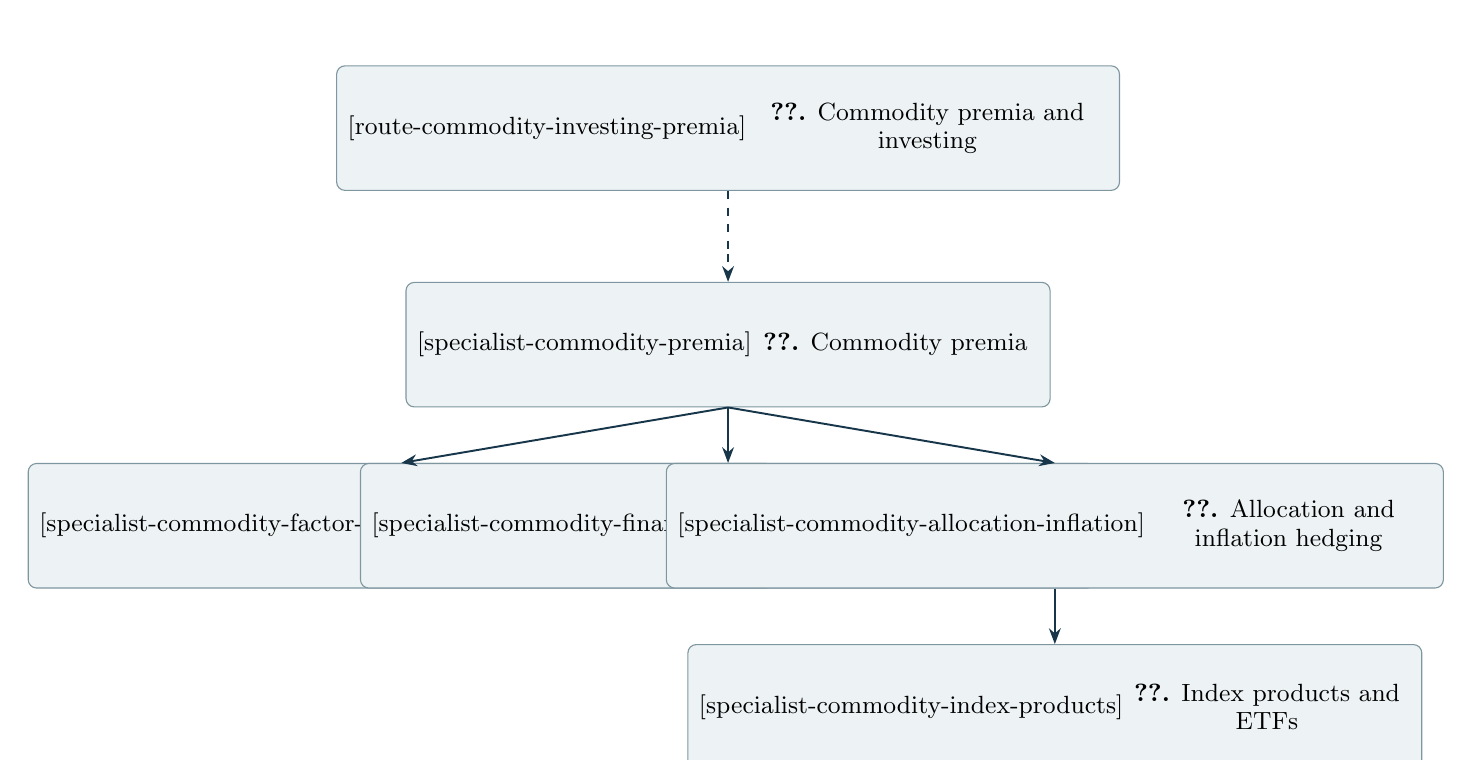
\begin{tikzpicture}[x=1cm,y=1cm]
\node[pathnode] (commodity-investing-premia) at (4.15,0) {\MeasurePathNode{4.6cm}{\textbf{\ref*{route-commodity-investing-premia}.} Commodity premia and investing}\hyperref[route-commodity-investing-premia]{\parbox[c][\pathnodeheight][c]{4.6cm}{\centering \textbf{\ref*{route-commodity-investing-premia}.} Commodity premia and investing}}};
\node[pathnode] (commodity-premia) at (4.15,-2.75) {\MeasurePathNode{3.65cm}{\textbf{\ref*{specialist-commodity-premia}.} Commodity premia}\hyperref[specialist-commodity-premia]{\parbox[c][\pathnodeheight][c]{3.65cm}{\centering \textbf{\ref*{specialist-commodity-premia}.} Commodity premia}}};
\node[pathnode] (commodity-factor-strategies) at (0.00,-5.05) {\MeasurePathNode{3.65cm}{\textbf{\ref*{specialist-commodity-factor-strategies}.} Commodity factor strategies}\hyperref[specialist-commodity-factor-strategies]{\parbox[c][\pathnodeheight][c]{3.65cm}{\centering \textbf{\ref*{specialist-commodity-factor-strategies}.} Commodity factor strategies}}};
\node[pathnode] (commodity-financialisation) at (4.15,-5.05) {\MeasurePathNode{3.65cm}{\textbf{\ref*{specialist-commodity-financialisation}.} Financialisation and speculation}\hyperref[specialist-commodity-financialisation]{\parbox[c][\pathnodeheight][c]{3.65cm}{\centering \textbf{\ref*{specialist-commodity-financialisation}.} Financialisation and speculation}}};
\node[pathnode] (commodity-allocation-inflation) at (8.30,-5.05) {\MeasurePathNode{3.65cm}{\textbf{\ref*{specialist-commodity-allocation-inflation}.} Allocation and inflation hedging}\hyperref[specialist-commodity-allocation-inflation]{\parbox[c][\pathnodeheight][c]{3.65cm}{\centering \textbf{\ref*{specialist-commodity-allocation-inflation}.} Allocation and inflation hedging}}};
\node[pathnode] (commodity-index-products) at (8.30,-7.35) {\MeasurePathNode{3.65cm}{\textbf{\ref*{specialist-commodity-index-products}.} Index products and ETFs}\hyperref[specialist-commodity-index-products]{\parbox[c][\pathnodeheight][c]{3.65cm}{\centering \textbf{\ref*{specialist-commodity-index-products}.} Index products and ETFs}}};
\draw[entryline] (commodity-investing-premia.south) -- (4.15,-1.60);
\draw[entryline] (4.15,-1.60) -- (4.15,-1.60);
\draw[entryarrow] (4.15,-1.60) -- (commodity-premia.north);
\draw[patharrow] (commodity-premia.south) -- (commodity-factor-strategies.north);
\draw[patharrow] (commodity-premia.south) -- (commodity-financialisation.north);
\draw[patharrow] (commodity-premia.south) -- (commodity-allocation-inflation.north);
\draw[patharrow] (commodity-allocation-inflation.south) -- (commodity-index-products.north);
\end{tikzpicture}\end{center}
\textbf{Bring these foundations with you.}\begin{itemize}
\item \hyperref[specialist-commodity-storage-curves]{Theory of storage, convenience yield and inventories} --- needed by \hyperref[specialist-commodity-premia]{Commodity premia}.
\item \hyperref[specialist-macro-regimes-stock-bond]{Macro regimes, inflation and the stock–bond correlation} --- needed by \hyperref[specialist-commodity-allocation-inflation]{Allocation and inflation hedging}.
\end{itemize}\hyperref[learning-map]{Return to the whole-guide DAG.}
\Needspace{12\baselineskip}
\subsection{Commodity risk premia: hedging pressure, inventories and the basis}\label{specialist-commodity-premia}
\textbf{Specialist pathway.} In \hyperref[route-commodity-investing-premia]{Commodity risk premia and investing: factors, allocation and index products}.

\textbf{Outcome.} Separate spot, roll and risk premia in commodity futures, test normal backwardation and hedging-pressure theories, explain the premia with inventories, the basis and intermediary capital, and test whether they predict returns out of sample.

\textbf{Prerequisites.} Commodity risk premia and investing overview; the theory of storage (20.1); factor regressions.

\textbf{Review first.} \hyperref[route-commodity-investing-premia]{Commodity risk premia and investing: factors, allocation and index products}; \hyperref[specialist-commodity-storage-curves]{Theory of storage, convenience yield and inventories}.

\textbf{Required readings, in order}
\begin{enumerate}\raggedright
\Needspace{5\baselineskip}\item \href{institutional_quantitative_finance_reading_list.pdf\#cp-hirshleifer-1988}{David Hirshleifer, ``Residual Risk, Trading Costs, and Commodity Futures Risk Premia''}\CataloguePage{327}\NoteKey{cp-hirshleifer-1988}\par \textbf{Theory.} See how participation costs for speculators create a premium for residual risk.
\Needspace{5\baselineskip}\item \href{institutional_quantitative_finance_reading_list.pdf\#ec-hirshleifer-1990}{David Hirshleifer, ``Hedging Pressure and Futures Price Movements in a General Equilibrium Model''}\CataloguePage{323}\NoteKey{ec-hirshleifer-1990}\par \textbf{Theory.} Derive futures risk premia from hedging pressure when hedgers face non-marketable risks.
\Needspace{5\baselineskip}\item \href{institutional_quantitative_finance_reading_list.pdf\#cp-ekeland-2019}{Ivar Ekeland, Delphine Lautier and Bertrand Villeneuve, ``Hedging pressure and speculation in commodity markets''}\CataloguePage{327}\NoteKey{cp-ekeland-2019}\par \textbf{Theory.} Nest the hedging-pressure and storage theories in one equilibrium model of physical and futures markets.
\Needspace{5\baselineskip}\item \href{institutional_quantitative_finance_reading_list.pdf\#cp-carter-rausser-schmitz-1983}{Colin A. Carter, Gordon C. Rausser and Andrew Schmitz, ``Efficient Asset Portfolios and the Theory of Normal Backwardation''}\CataloguePage{326}\NoteKey{cp-carter-rausser-schmitz-1983}\par \textbf{Evidence.} Correct Dusak's CAPM test for speculators' net positions and for futures in the market portfolio.
\Needspace{5\baselineskip}\item \href{institutional_quantitative_finance_reading_list.pdf\#cp-chang-1985}{Eric C. Chang, ``Returns to Speculators and the Theory of Normal Backwardation''}\CataloguePage{327}\NoteKey{cp-chang-1985}\par \textbf{Evidence.} Test normal backwardation with the returns to speculators in grain futures.
\Needspace{5\baselineskip}\item \href{institutional_quantitative_finance_reading_list.pdf\#ec-bessembinder-1992}{Hendrik Bessembinder, ``Systematic Risk, Hedging Pressure, and Risk Premiums in Futures Markets''}\CataloguePage{323}\NoteKey{ec-bessembinder-1992}\par \textbf{Evidence.} Show that net hedging moves futures returns beyond systematic risk.
\Needspace{5\baselineskip}\item \href{institutional_quantitative_finance_reading_list.pdf\#cp-bessembinder-chan-1992}{Hendrik Bessembinder and Kalok Chan, ``Time-varying risk premia and forecastable returns in futures markets''}\CataloguePage{327}\NoteKey{cp-bessembinder-chan-1992}\par \textbf{Evidence.} See the instruments that forecast stock and bond returns also forecast futures returns.
\Needspace{5\baselineskip}\item \href{institutional_quantitative_finance_reading_list.pdf\#ec-deroon-nijman-veld-2000}{Frans A. de Roon, Theo E. Nijman and Chris Veld, ``Hedging Pressure Effects in Futures Markets''}\CataloguePage{324}\NoteKey{ec-deroon-nijman-veld-2000}\par \textbf{Evidence.} Measure own-market and cross-market hedging-pressure effects in twenty futures markets.
\Needspace{5\baselineskip}\item \href{institutional_quantitative_finance_reading_list.pdf\#catalogue-0242}{Gary Gorton, Fumio Hayashi and K. Geert Rouwenhorst, ``The Fundamentals of Commodity Futures Returns''}\CataloguePage{322}\NoteKey{catalogue-0242}\par \textbf{Evidence.} Link premia to inventories, the basis and past returns.
\Needspace{5\baselineskip}\item \href{institutional_quantitative_finance_reading_list.pdf\#wide-szymanowska-premia}{Marta Szymanowska, Frans de Roon, Theo Nijman and Rob van den Goorbergh, ``An Anatomy of Commodity Futures Risk Premia''}\CataloguePage{323}\NoteKey{wide-szymanowska-premia}\par \textbf{Evidence.} Decompose spot and term premia with basis-sorted portfolios.
\Needspace{5\baselineskip}\item \href{institutional_quantitative_finance_reading_list.pdf\#wide-basu-miffre}{Devraj Basu and Joëlle Miffre, ``Capturing the risk premium of commodity futures: The role of hedging pressure''}\CataloguePage{323}\NoteKey{wide-basu-miffre}\par \textbf{Evidence.} Use hedging pressure as a long--short signal.
\Needspace{5\baselineskip}\item \href{institutional_quantitative_finance_reading_list.pdf\#ec-acharya-lochstoer-ramadorai-2013}{Viral V. Acharya, Lars A. Lochstoer and Tarun Ramadorai, ``Limits to Arbitrage and Hedging: Evidence from Commodity Markets''}\CataloguePage{324}\NoteKey{ec-acharya-lochstoer-ramadorai-2013}\par \textbf{Evidence.} Connect producers' default risk to hedging demand, futures premia and inventories.
\Needspace{5\baselineskip}\item \href{institutional_quantitative_finance_reading_list.pdf\#ec-kang-rouwenhorst-tang-2020}{Wenjin Kang, K. Geert Rouwenhorst and Ke Tang, ``A Tale of Two Premiums: The Role of Hedgers and Speculators in Commodity Futures Markets''}\CataloguePage{324}\NoteKey{ec-kang-rouwenhorst-tang-2020}\par \textbf{Evidence.} Separate the liquidity premium earned by short-term speculators from the hedging premium paid by hedgers.
\Needspace{5\baselineskip}\item \href{institutional_quantitative_finance_reading_list.pdf\#ec-etula-2013}{Erkko Etula, ``Broker-Dealer Risk Appetite and Commodity Returns''}\CataloguePage{324}\NoteKey{ec-etula-2013}\par \textbf{Evidence.} See broker-dealer risk appetite forecast commodity returns.
\Needspace{5\baselineskip}\item \href{institutional_quantitative_finance_reading_list.pdf\#ec-hong-yogo-2012}{Harrison Hong and Motohiro Yogo, ``What Does Futures Market Interest Tell Us about the Macroeconomy and Asset Prices?''}\CataloguePage{324}\NoteKey{ec-hong-yogo-2012}\par \textbf{Evidence.} Use open-interest growth to predict commodity returns and economic activity.
\Needspace{5\baselineskip}\item \href{institutional_quantitative_finance_reading_list.pdf\#ec-hamilton-wu-2014}{James D. Hamilton and Jing Cynthia Wu, ``Risk Premia in Crude Oil Futures Prices''}\CataloguePage{324}\NoteKey{ec-hamilton-wu-2014}\par \textbf{Evidence.} Estimate risk premia in crude-oil futures with an affine model and see how they changed after 2005.
\end{enumerate}
\Needspace{5\baselineskip}\textbf{Checkpoint.} For about 25 commodity futures since 1990, compute monthly excess returns from a documented roll schedule and split them into spot and term components. Sort into portfolios on the basis, on hedging pressure from the CFTC reports and on open-interest growth, estimate the premia with and without 2005--08, and test whether the Treasury-bill yield and the default spread forecast the equal-weight excess return. Report which signals survive transaction costs and which reduce to the basis.

\textbf{Optional branches.} \href{institutional_quantitative_finance_reading_list.pdf\#ec-dusak-1973}{Test commodity premia against the CAPM.}\BranchPage{325} \href{institutional_quantitative_finance_reading_list.pdf\#ec-dewally-2013}{See which trader types earn profits in energy futures.}\BranchPage{324} \href{institutional_quantitative_finance_reading_list.pdf\#cp-brooks-prokopczuk-wu-2013}{Check the stability of storage and risk-premium evidence over time.}\BranchPage{327}
\par{\small \hyperref[learning-map]{Learning pathway DAG} \textbar{} \hyperref[route-commodity-investing-premia]{Section overview} \textbar{} \hyperref[map-commodity-investing-premia]{Section DAG}\NoteKey{commodity-premia}}
\Needspace{12\baselineskip}
\subsection{Commodity factor strategies: carry, momentum, trend, curve and skewness}\label{specialist-commodity-factor-strategies}
\textbf{Specialist pathway.} In \hyperref[route-commodity-investing-premia]{Commodity risk premia and investing: factors, allocation and index products}.

\textbf{Outcome.} Build carry, momentum, trend, basis-momentum, curve-momentum and skewness portfolios in commodity futures with realistic roll schedules, evaluate them with commodity factor models and the wider anomaly evidence, and check which survive costs and less frequent rebalancing.

\textbf{Prerequisites.} Commodity risk premia: hedging pressure, inventories and the basis; cross-sectional and time-series momentum.

\textbf{Review first.} \hyperref[specialist-commodity-premia]{Commodity risk premia: hedging pressure, inventories and the basis}.

\textbf{Required readings, in order}
\begin{enumerate}\raggedright
\Needspace{5\baselineskip}\item \href{institutional_quantitative_finance_reading_list.pdf\#ec-miffre-2016}{Joëlle Miffre, ``Long-Short Commodity Investing: A Review of the Literature''}\CataloguePage{325}\NoteKey{ec-miffre-2016}\par \textbf{Foundations.} Survey long--short commodity strategies and the premia they collect.
\Needspace{5\baselineskip}\item \href{institutional_quantitative_finance_reading_list.pdf\#ec-miffre-rallis-2007}{Joëlle Miffre and Georgios Rallis, ``Momentum Strategies in Commodity Futures Markets''}\CataloguePage{325}\NoteKey{ec-miffre-rallis-2007}\par \textbf{Evidence.} Test cross-sectional momentum across commodity futures.
\Needspace{5\baselineskip}\item \href{institutional_quantitative_finance_reading_list.pdf\#ec-fuertes-miffre-rallis-2010}{Ana-Maria Fuertes, Joëlle Miffre and Georgios Rallis, ``Tactical Allocation in Commodity Futures Markets: Combining Momentum and Term Structure Signals''}\CataloguePage{325}\NoteKey{ec-fuertes-miffre-rallis-2010}\par \textbf{Evidence.} Combine momentum and term-structure signals.
\Needspace{5\baselineskip}\item \href{institutional_quantitative_finance_reading_list.pdf\#cp-szakmary-2010}{Andrew C. Szakmary, Qian Shen and Subhash C. Sharma, ``Trend-following trading strategies in commodity futures: A re-examination''}\CataloguePage{327}\NoteKey{cp-szakmary-2010}\par \textbf{Evidence.} Test moving-average and channel trend rules across 28 commodities over 48 years.
\Needspace{5\baselineskip}\item \href{institutional_quantitative_finance_reading_list.pdf\#alpha-carry}{Ralph Koijen, Tobias Moskowitz, Lasse Heje Pedersen and Evert Vrugt, ``Carry''}\CataloguePage{30}\NoteKey{alpha-carry}\par \textbf{Evidence.} Compare commodity carry with carry in other asset classes.
\Needspace{5\baselineskip}\item \href{institutional_quantitative_finance_reading_list.pdf\#alpha-value}{Clifford Asness, Tobias Moskowitz and Lasse Heje Pedersen, ``Value and Momentum Everywhere'' (author copy)}\CataloguePage{192}\NoteKey{alpha-value}\par \textbf{Evidence.} Add commodity value, measured as long-horizon reversal, alongside momentum across asset classes.
\Needspace{5\baselineskip}\item \href{institutional_quantitative_finance_reading_list.pdf\#ec-yang-2013}{Fan Yang, ``Investment Shocks and the Commodity Basis Spread''}\CataloguePage{326}\NoteKey{ec-yang-2013}\par \textbf{Evidence.} Explain the basis spread with investment shocks.
\Needspace{5\baselineskip}\item \href{institutional_quantitative_finance_reading_list.pdf\#wide-bakshi-gao-rossi}{Gurdip Bakshi, Xiaohui Gao and Alberto G. Rossi, ``Understanding the Sources of Risk Underlying the Cross Section of Commodity Returns''}\CataloguePage{323}\NoteKey{wide-bakshi-gao-rossi}\par \textbf{Evidence.} Price commodity returns with average, carry and momentum factors.
\Needspace{5\baselineskip}\item \href{institutional_quantitative_finance_reading_list.pdf\#ec-daskalaki-2014}{Charoula Daskalaki, Alexandros Kostakis and George Skiadopoulos, ``Are There Common Factors in Individual Commodity Futures Returns?''}\CataloguePage{326}\NoteKey{ec-daskalaki-2014}\par \textbf{Evidence.} Test whether equity-style and macro factors price individual commodity futures.
\Needspace{5\baselineskip}\item \href{institutional_quantitative_finance_reading_list.pdf\#cp-christoffersen-lunde-olesen-2019}{Peter Christoffersen, Asger Lunde and Kasper V. Olesen, ``Factor Structure in Commodity Futures Return and Volatility''}\CataloguePage{328}\NoteKey{cp-christoffersen-lunde-olesen-2019}\par \textbf{Evidence.} Contrast the weak factor structure in returns with the strong one in volatility.
\Needspace{5\baselineskip}\item \href{institutional_quantitative_finance_reading_list.pdf\#ec-boons-prado-2019}{Martijn Boons and Melissa Porras Prado, ``Basis-Momentum''}\CataloguePage{326}\NoteKey{ec-boons-prado-2019}\par \textbf{Evidence.} Use basis-momentum, momentum in the slope of the curve, as a predictor.
\Needspace{5\baselineskip}\item \href{institutional_quantitative_finance_reading_list.pdf\#cp-paschke-2020}{Raphael Paschke, Marcel Prokopczuk and Chardin Wese Simen, ``Curve momentum''}\CataloguePage{327}\NoteKey{cp-paschke-2020}\par \textbf{Evidence.} Trade momentum within each futures curve rather than across commodities.
\Needspace{5\baselineskip}\item \href{institutional_quantitative_finance_reading_list.pdf\#ec-fernandez-perez-skewness-2018}{Adrian Fernandez-Perez, Bart Frijns, Ana-Maria Fuertes and Joëlle Miffre, ``The Skewness of Commodity Futures Returns''}\CataloguePage{326}\NoteKey{ec-fernandez-perez-skewness-2018}\par \textbf{Evidence.} Sort commodities on the skewness of their returns.
\Needspace{5\baselineskip}\item \href{institutional_quantitative_finance_reading_list.pdf\#cp-hollstein-2021}{Fabian Hollstein, Marcel Prokopczuk and Björn Tharann, ``Anomalies in Commodity Futures Markets''}\CataloguePage{328}\NoteKey{cp-hollstein-2021}\par \textbf{Validation.} Check which equity anomalies are priced in commodities and how premia fade with annual rebalancing.
\end{enumerate}
\Needspace{5\baselineskip}\textbf{Checkpoint.} Using a roll schedule that avoids delivery months, build monthly long--short quintile portfolios on the basis, twelve-month momentum, a moving-average trend rule, basis-momentum, curve momentum and skewness for about 25 commodities since 1990. Report Sharpe ratios, turnover, drawdowns and alphas against the Bakshi--Gao--Rossi factors, then repeat with annual rebalancing and after costs, and report which signals add to carry and momentum.

\textbf{Optional branches.} \href{institutional_quantitative_finance_reading_list.pdf\#exp-gu-relative-basis-commodity}{Use relative basis as a signal.}\BranchPage{322} \href{institutional_quantitative_finance_reading_list.pdf\#w4-qian-commodity-factor-momentum}{Test factor momentum in commodity factors.}\BranchPage{323} \href{institutional_quantitative_finance_reading_list.pdf\#ec-bianchi-drew-fan-2015}{Combine momentum with long-horizon reversal.}\BranchPage{326} \href{institutional_quantitative_finance_reading_list.pdf\#w4-sakkas-commodity-premia}{Compare commodity risk-premium measures and their drivers.}\BranchPage{323} \href{institutional_quantitative_finance_reading_list.pdf\#s6-tsmom}{Compare with time-series momentum across asset classes.}\BranchPage{30} \href{institutional_quantitative_finance_reading_list.pdf\#cp-fernandez-perez-ivol-2016}{See idiosyncratic volatility lose its price once backwardation and contango are modelled.}\BranchPage{328}
\par{\small \hyperref[learning-map]{Learning pathway DAG} \textbar{} \hyperref[route-commodity-investing-premia]{Section overview} \textbar{} \hyperref[map-commodity-investing-premia]{Section DAG}\NoteKey{commodity-factor-strategies}}
\Needspace{12\baselineskip}
\subsection{Financialisation, speculation and index investing in commodity markets}\label{specialist-commodity-financialisation}
\textbf{Specialist pathway.} In \hyperref[route-commodity-investing-premia]{Commodity risk premia and investing: factors, allocation and index products}.

\textbf{Outcome.} Weigh the evidence on whether index investors and speculators moved commodity prices, correlations and volatility; read CFTC trader-classification data correctly; test speculation claims against inventories and structural oil-market models; and separate price effects from information and real effects.

\textbf{Prerequisites.} Commodity risk premia: hedging pressure, inventories and the basis; panel regression and Granger-causality tests.

\textbf{Review first.} \hyperref[specialist-commodity-premia]{Commodity risk premia: hedging pressure, inventories and the basis}.

\textbf{Required readings, in order}
\begin{enumerate}\raggedright
\Needspace{5\baselineskip}\item \href{institutional_quantitative_finance_reading_list.pdf\#ec-fattouh-kilian-mahadeva-2013}{Bassam Fattouh, Lutz Kilian and Lavan Mahadeva, ``The Role of Speculation in Oil Markets: What Have We Learned So Far?''}\CataloguePage{340}\NoteKey{ec-fattouh-kilian-mahadeva-2013}\par \textbf{Foundations.} Survey what is known about speculation in oil markets.
\Needspace{5\baselineskip}\item \href{institutional_quantitative_finance_reading_list.pdf\#cp-masters-2008}{Michael W. Masters, Testimony before the U.S. Senate Committee on Homeland Security and Governmental Affairs, 20 May 2008}\CataloguePage{342}\NoteKey{cp-masters-2008}\par \textbf{Foundations.} Read the claim, made to the Senate in 2008, that later tests examine.
\Needspace{5\baselineskip}\item \href{institutional_quantitative_finance_reading_list.pdf\#ec-cftc-cot}{U.S. Commodity Futures Trading Commission, Commitments of Traders: explanatory notes and Disaggregated COT explanatory notes}\CataloguePage{340}\NoteKey{ec-cftc-cot}\par \textbf{Data.} Read how the legacy and disaggregated reports classify traders, and what they cannot show.
\Needspace{5\baselineskip}\item \href{institutional_quantitative_finance_reading_list.pdf\#wide-tang-xiong-index}{Ke Tang and Wei Xiong, ``Index Investment and the Financialization of Commodities''}\CataloguePage{338}\NoteKey{wide-tang-xiong-index}\par \textbf{Evidence.} See index-investor correlation effects.
\Needspace{5\baselineskip}\item \href{institutional_quantitative_finance_reading_list.pdf\#ec-irwin-sanders-2011}{Scott H. Irwin and Dwight R. Sanders, ``Index Funds, Financialization, and Commodity Futures Markets''}\CataloguePage{338}\NoteKey{ec-irwin-sanders-2011}\par \textbf{Evidence.} Review index-fund positions and the case that they did not drive prices.
\Needspace{5\baselineskip}\item \href{institutional_quantitative_finance_reading_list.pdf\#ec-irwin-sanders-2012}{Scott H. Irwin and Dwight R. Sanders, ``Testing the Masters Hypothesis in Commodity Futures Markets''}\CataloguePage{339}\NoteKey{ec-irwin-sanders-2012}\par \textbf{Evidence.} Test the Masters hypothesis with index and swap-dealer positions.
\Needspace{5\baselineskip}\item \href{institutional_quantitative_finance_reading_list.pdf\#ec-hamilton-wu-2015}{James D. Hamilton and Jing Cynthia Wu, ``Effects of Index-Fund Investing on Commodity Futures Prices''}\CataloguePage{339}\NoteKey{ec-hamilton-wu-2015}\par \textbf{Evidence.} Test whether index positions predict futures returns.
\Needspace{5\baselineskip}\item \href{institutional_quantitative_finance_reading_list.pdf\#ec-singleton-2014}{Kenneth J. Singleton, ``Investor Flows and the 2008 Boom/Bust in Oil Prices''}\CataloguePage{339}\NoteKey{ec-singleton-2014}\par \textbf{Evidence.} See investor flows predict oil futures returns around the 2008 boom and bust.
\Needspace{5\baselineskip}\item \href{institutional_quantitative_finance_reading_list.pdf\#ec-buyuksahin-harris-2011}{Bahattin Büyükşahin and Jeffrey H. Harris, ``Do Speculators Drive Crude Oil Futures Prices?''}\CataloguePage{339}\NoteKey{ec-buyuksahin-harris-2011}\par \textbf{Evidence.} Test whether speculators' positions lead crude-oil prices.
\Needspace{5\baselineskip}\item \href{institutional_quantitative_finance_reading_list.pdf\#ec-henderson-pearson-wang-2015}{Brian J. Henderson, Neil D. Pearson and Li Wang, ``New Evidence on the Financialization of Commodity Markets''}\CataloguePage{339}\NoteKey{ec-henderson-pearson-wang-2015}\par \textbf{Evidence.} Use commodity-linked note issuance as a flow shock unrelated to news.
\Needspace{5\baselineskip}\item \href{institutional_quantitative_finance_reading_list.pdf\#ec-cheng-kirilenko-xiong-2015}{Ing-Haw Cheng, Andrei Kirilenko and Wei Xiong, ``Convective Risk Flows in Commodity Futures Markets''}\CataloguePage{339}\NoteKey{ec-cheng-kirilenko-xiong-2015}\par \textbf{Evidence.} See financial traders cut positions in a crisis and pass risk back to hedgers.
\Needspace{5\baselineskip}\item \href{institutional_quantitative_finance_reading_list.pdf\#cp-buyuksahin-robe-2014}{Bahattin Büyükşahin and Michel A. Robe, ``Speculators, commodities and cross-market linkages''}\CataloguePage{341}\NoteKey{cp-buyuksahin-robe-2014}\par \textbf{Evidence.} See hedge-fund participation, not index trading, predict commodity--equity correlation.
\Needspace{5\baselineskip}\item \href{institutional_quantitative_finance_reading_list.pdf\#cp-knittel-pindyck-2016}{Christopher R. Knittel and Robert S. Pindyck, ``The Simple Economics of Commodity Price Speculation''}\CataloguePage{340}\NoteKey{cp-knittel-pindyck-2016}\par \textbf{Evidence.} Check whether speculation fits the data on production, inventories and convenience yields.
\Needspace{5\baselineskip}\item \href{institutional_quantitative_finance_reading_list.pdf\#physical-kilian-murphy-oil-2014}{Lutz Kilian and Daniel P. Murphy, The Role of Inventories and Speculative Trading in the Global Market for Crude Oil}\CataloguePage{338}\NoteKey{physical-kilian-murphy-oil-2014}\par \textbf{Evidence.} Bound the role of speculative oil inventories in a structural model.
\Needspace{5\baselineskip}\item \href{institutional_quantitative_finance_reading_list.pdf\#cp-juvenal-petrella-2015}{Luciana Juvenal and Ivan Petrella, ``Speculation in the Oil Market''}\CataloguePage{341}\NoteKey{cp-juvenal-petrella-2015}\par \textbf{Evidence.} Identify speculative oil shocks with a dynamic factor model.
\Needspace{5\baselineskip}\item \href{institutional_quantitative_finance_reading_list.pdf\#ec-sockin-xiong-2015}{Michael Sockin and Wei Xiong, ``Informational Frictions and Commodity Markets''}\CataloguePage{339}\NoteKey{ec-sockin-xiong-2015}\par \textbf{Theory.} Model how prices that carry information about demand can feed back into demand.
\Needspace{5\baselineskip}\item \href{institutional_quantitative_finance_reading_list.pdf\#ec-basak-pavlova-2016}{Suleyman Basak and Anna Pavlova, ``A Model of Financialization of Commodities''}\CataloguePage{340}\NoteKey{ec-basak-pavlova-2016}\par \textbf{Theory.} Model how index investors raise prices, volatilities and correlations.
\end{enumerate}
\Needspace{5\baselineskip}\textbf{Checkpoint.} Merge weekly disaggregated COT positions, and the supplemental index-trader positions for agricultural markets, with front-month returns for crude oil, natural gas, corn and copper since 2006. Test whether changes in managed-money and swap-dealer positions predict returns and realised volatility, then repeat around a predictable flow such as an index rebalancing. State what the trader classification cannot identify, whether any effect survives controls for the basis and macroeconomic news, and whether inventories show the build-up that a speculative price effect would require.

\textbf{Optional branches.} \href{institutional_quantitative_finance_reading_list.pdf\#ec-brunetti-2016}{Test whether speculators raise or lower volatility in crude oil, natural gas and corn.}\BranchPage{339} \href{institutional_quantitative_finance_reading_list.pdf\#ec-brogaard-2019}{Measure the real costs of index investing for firms that use commodities.}\BranchPage{340} \href{institutional_quantitative_finance_reading_list.pdf\#ec-goldstein-yang-2022}{Model how financialisation changes the information in futures prices.}\BranchPage{340} \href{institutional_quantitative_finance_reading_list.pdf\#w3-martin-steel-futures}{See real effects of introducing futures.}\BranchPage{368} \href{institutional_quantitative_finance_reading_list.pdf\#cp-kilian-lee-2014}{Put a dollar figure on the speculative component of the real oil price.}\BranchPage{340} \href{institutional_quantitative_finance_reading_list.pdf\#cp-adams-gluck-2015}{See commodity--equity spillovers persist after the financial crisis.}\BranchPage{341} \href{institutional_quantitative_finance_reading_list.pdf\#cp-le-pen-sevi-2018}{Link excess comovement of unrelated commodities to speculative intensity.}\BranchPage{341} \href{institutional_quantitative_finance_reading_list.pdf\#cp-baker-2021}{Model financialisation with storage and see it lower the futures premium without raising mean spot prices.}\BranchPage{341} \href{institutional_quantitative_finance_reading_list.pdf\#cp-main-2018}{Check whether long-only risk premiums fell after financialisation.}\BranchPage{341} \href{institutional_quantitative_finance_reading_list.pdf\#cp-bruno-2017}{Separate business-cycle and speculative drivers of agriculture--equity comovement.}\BranchPage{341}
\par{\small \hyperref[learning-map]{Learning pathway DAG} \textbar{} \hyperref[route-commodity-investing-premia]{Section overview} \textbar{} \hyperref[map-commodity-investing-premia]{Section DAG}\NoteKey{commodity-financialisation}}
\Needspace{12\baselineskip}
\subsection{Commodities in multi-asset portfolios: diversification and inflation hedging}\label{specialist-commodity-allocation-inflation}
\textbf{Specialist pathway.} In \hyperref[route-commodity-investing-premia]{Commodity risk premia and investing: factors, allocation and index products}.

\textbf{Outcome.} Judge whether commodities improve a stock--bond portfolio in and out of sample, measure their inflation-hedging properties by horizon and regime, and decide between long-only exposure and commodity factor premia in a strategic allocation.

\textbf{Prerequisites.} Commodity risk premia: hedging pressure, inventories and the basis (23.1); Macro regimes, inflation and the stock--bond correlation (12.5), whose inflation-hedging readings this pathway builds on; mean-variance and risk-parity portfolio construction.

\textbf{Review first.} \hyperref[specialist-commodity-premia]{Commodity risk premia: hedging pressure, inventories and the basis}; \hyperref[specialist-macro-regimes-stock-bond]{Macro regimes, inflation and the stock–bond correlation}.

\textbf{Required readings, in order}
\begin{enumerate}\raggedright
\Needspace{5\baselineskip}\item \href{institutional_quantitative_finance_reading_list.pdf\#cp-bodie-1981}{Zvi Bodie, ``Investment Strategy in an Inflationary Environment''}\CataloguePage{342}\NoteKey{cp-bodie-1981}\par \textbf{Foundations.} Start with the case that commodity futures, the only asset positively correlated with inflation, lower the risk of a real-return portfolio.
\Needspace{5\baselineskip}\item \href{institutional_quantitative_finance_reading_list.pdf\#cp-greer-2000}{Robert J. Greer, ``The Nature of Commodity Index Returns''}\CataloguePage{342}\NoteKey{cp-greer-2000}\par \textbf{Foundations.} Read the practitioner case for a long-only index: equity-like returns, positive skew and negative correlation with stocks and bonds.
\Needspace{5\baselineskip}\item \href{institutional_quantitative_finance_reading_list.pdf\#cp-jensen-johnson-mercer-2000}{Gerald R. Jensen, Robert R. Johnson and Jeffrey M. Mercer, ``Efficient use of commodity futures in diversified portfolios''}\CataloguePage{342}\NoteKey{cp-jensen-johnson-mercer-2000}\par \textbf{Evidence.} See the optimal commodity weight depend on whether monetary policy is restrictive or expansive.
\Needspace{5\baselineskip}\item \href{institutional_quantitative_finance_reading_list.pdf\#cp-daskalaki-skiadopoulos-2011}{Charoula Daskalaki and George Skiadopoulos, ``Should investors include commodities in their portfolios after all? New evidence''}\CataloguePage{343}\NoteKey{cp-daskalaki-skiadopoulos-2011}\par \textbf{Evidence.} See in-sample diversification gains disappear out of sample.
\Needspace{5\baselineskip}\item \href{institutional_quantitative_finance_reading_list.pdf\#cp-belousova-dorfleitner-2012}{Julia Belousova and Gregor Dorfleitner, ``On the diversification benefits of commodities from the perspective of euro investors''}\CataloguePage{343}\NoteKey{cp-belousova-dorfleitner-2012}\par \textbf{Evidence.} Separate risk reduction from return enhancement by commodity group for a euro investor.
\Needspace{5\baselineskip}\item \href{institutional_quantitative_finance_reading_list.pdf\#cp-bessler-wolff-2015}{Wolfgang Bessler and Dominik Wolff, ``Do commodities add value in multi-asset portfolios? An out-of-sample analysis for different investment strategies''}\CataloguePage{343}\NoteKey{cp-bessler-wolff-2015}\par \textbf{Evidence.} Compare the out-of-sample gains across allocation rules, from equal weights to Black--Litterman.
\Needspace{5\baselineskip}\item \href{institutional_quantitative_finance_reading_list.pdf\#cp-gao-nardari-2018}{Xin Gao and Federico Nardari, ``Do Commodities Add Economic Value in Asset Allocation? New Evidence from Time-Varying Moments''}\CataloguePage{343}\NoteKey{cp-gao-nardari-2018}\par \textbf{Evidence.} Recover economic value from commodities when the allocation exploits predictable moments.
\Needspace{5\baselineskip}\item \href{institutional_quantitative_finance_reading_list.pdf\#ec-levine-2018}{Ari Levine, Yao Hua Ooi, Matthew Richardson and Caroline Sasseville, ``Commodities for the Long Run''}\CataloguePage{325}\NoteKey{ec-levine-2018}\par \textbf{Evidence.} Put the premium and its behaviour across inflation and growth states in data back to 1877.
\Needspace{5\baselineskip}\item \href{institutional_quantitative_finance_reading_list.pdf\#ec-bhardwaj-gorton-rouwenhorst-2015}{Geetesh Bhardwaj, Gary B. Gorton and K. Geert Rouwenhorst, ``Facts and Fantasies about Commodity Futures Ten Years Later''}\CataloguePage{325}\NoteKey{ec-bhardwaj-gorton-rouwenhorst-2015}\par \textbf{Evidence.} Check the original facts out of sample ten years later.
\Needspace{5\baselineskip}\item \href{institutional_quantitative_finance_reading_list.pdf\#cp-roache-attie-2009}{Shaun Roache and Alexander Attie, ``Inflation Hedging for Long-Term Investors''}\CataloguePage{343}\NoteKey{cp-roache-attie-2009}\par \textbf{Evidence.} See commodities hedge inflation surprises in the short run but not necessarily over long horizons.
\Needspace{5\baselineskip}\item \href{institutional_quantitative_finance_reading_list.pdf\#cp-gospodinov-ng-2013}{Nikolay Gospodinov and Serena Ng, ``Commodity Prices, Convenience Yields, and Inflation''}\CataloguePage{343}\NoteKey{cp-gospodinov-ng-2013}\par \textbf{Evidence.} Use commodity convenience yields to forecast inflation.
\Needspace{5\baselineskip}\item \href{institutional_quantitative_finance_reading_list.pdf\#cp-blitz-de-groot-2014}{David Blitz and Wilma de Groot, ``Strategic Allocation to Commodity Factor Premiums''}\CataloguePage{344}\NoteKey{cp-blitz-de-groot-2014}\par \textbf{Implementation.} Weigh commodity factor premia against the long-only market portfolio in the strategic mix.
\end{enumerate}
\Needspace{5\baselineskip}\textbf{Checkpoint.} Using monthly returns since 1970 for US equities, Treasuries, bills, an equal-weight commodity futures index and a long--short commodity factor portfolio, run mean-variance spanning tests in sample, then form rolling minimum-variance, risk-parity and mean-variance portfolios with and without commodities and evaluate them out of sample after costs. Regress each asset's real return on unexpected inflation at 1-, 12- and 60-month horizons and report the hedge ratios separately for 1970--85, 1986--2020 and 2021 onward.

\textbf{Optional branches.} \href{institutional_quantitative_finance_reading_list.pdf\#cp-cheung-miu-2010}{Test whether the diversification gain is statistically significant and survives bear-market regimes.}\BranchPage{342} \href{institutional_quantitative_finance_reading_list.pdf\#ma-ilmanen-maloney-ross-2014}{Compare how asset classes and style premia respond to growth and inflation environments.}\BranchPage{269} \href{institutional_quantitative_finance_reading_list.pdf\#cp-bampinas-panagiotidis-2015}{Check gold and silver as long-run inflation hedges over two centuries.}\BranchPage{343} \href{institutional_quantitative_finance_reading_list.pdf\#ec-erb-harvey-2013}{Weigh gold's reputation as an inflation hedge against its high real price.}\BranchPage{321}
\par{\small \hyperref[learning-map]{Learning pathway DAG} \textbar{} \hyperref[route-commodity-investing-premia]{Section overview} \textbar{} \hyperref[map-commodity-investing-premia]{Section DAG}\NoteKey{commodity-allocation-inflation}}
\Needspace{12\baselineskip}
\subsection{Commodity index products: index rules, roll costs, ETFs and flow effects}\label{specialist-commodity-index-products}
\textbf{Specialist pathway.} In \hyperref[route-commodity-investing-premia]{Commodity risk premia and investing: factors, allocation and index products}.

\textbf{Outcome.} Read a commodity index methodology, estimate what predictable rolls and ETF rebalancing cost, compare enhanced indices with traditional ones, and judge whether index and ETF flows move futures prices.

\textbf{Prerequisites.} Commodities in multi-asset portfolios (23.4); futures rolls and calendar spreads from the theory of storage (20.1).

\textbf{Review first.} \hyperref[specialist-commodity-allocation-inflation]{Commodities in multi-asset portfolios: diversification and inflation hedging}.

\textbf{Required readings, in order}
\begin{enumerate}\raggedright
\Needspace{5\baselineskip}\item \href{institutional_quantitative_finance_reading_list.pdf\#ec-erb-harvey-2016}{Claude B. Erb and Campbell R. Harvey, ``Conquering Misperceptions about Commodity Futures Investing''}\CataloguePage{325}\NoteKey{ec-erb-harvey-2016}\par \textbf{Foundations.} Correct common misperceptions about roll yield and inflation hedging before judging an index.
\Needspace{5\baselineskip}\item \href{institutional_quantitative_finance_reading_list.pdf\#cp-bcom-methodology-2026}{Bloomberg Index Services Limited, The Bloomberg Commodity Index Methodology}\CataloguePage{345}\NoteKey{cp-bcom-methodology-2026}\par \textbf{Data.} Read the actual weighting rules, diversification caps and roll window of a benchmark index.
\Needspace{5\baselineskip}\item \href{institutional_quantitative_finance_reading_list.pdf\#cp-cftc-index-traders-2008}{U.S. Commodity Futures Trading Commission, Staff Report on Commodity Swap Dealers \& Index Traders with Commission Recommendations}\CataloguePage{342}\NoteKey{cp-cftc-index-traders-2008}\par \textbf{Data.} Size index investment on and off exchange from the CFTC's 2008 special call.
\Needspace{5\baselineskip}\item \href{institutional_quantitative_finance_reading_list.pdf\#cp-guedj-li-mccann-2011}{Ilan Guedj, Guohua Li and Craig McCann, ``Futures-Based Commodity ETFs''}\CataloguePage{344}\NoteKey{cp-guedj-li-mccann-2011}\par \textbf{Mechanics.} Explain why futures-based oil ETFs drift away from spot price changes.
\Needspace{5\baselineskip}\item \href{institutional_quantitative_finance_reading_list.pdf\#cp-rallis-miffre-fuertes-2013}{Georgios Rallis, Joëlle Miffre and Ana-Maria Fuertes, ``Strategic and Tactical Roles of Enhanced Commodity Indices''}\CataloguePage{344}\NoteKey{cp-rallis-miffre-fuertes-2013}\par \textbf{Evidence.} Compare traditional indices with maturity-, momentum- and term-structure-enhanced versions.
\Needspace{5\baselineskip}\item \href{institutional_quantitative_finance_reading_list.pdf\#cp-stoll-whaley-2011}{Hans R. Stoll and Robert E. Whaley, ``Commodity Index Investing: Speculation or Diversification?''}\CataloguePage{344}\NoteKey{cp-stoll-whaley-2011}\par \textbf{Evidence.} See the case that index rolls and flows have little effect on futures prices.
\Needspace{5\baselineskip}\item \href{institutional_quantitative_finance_reading_list.pdf\#cp-irwin-garcia-good-kunda-2011}{Scott H. Irwin, Philip Garcia, Darrel L. Good and Eugene L. Kunda, ``Spreads and Non-Convergence in Chicago Board of Trade Corn, Soybean, and Wheat Futures: Are Index Funds to Blame?''}\CataloguePage{344}\NoteKey{cp-irwin-garcia-good-kunda-2011}\par \textbf{Evidence.} Test whether index rolls widened spreads and broke convergence in grain futures.
\Needspace{5\baselineskip}\item \href{institutional_quantitative_finance_reading_list.pdf\#cp-bgr-investor-interest-2016}{Geetesh Bhardwaj, Gary B. Gorton and K. Geert Rouwenhorst, ``Investor Interest and the Returns to Commodity Investing''}\CataloguePage{344}\NoteKey{cp-bgr-investor-interest-2016}\par \textbf{Evidence.} Check whether returns and correlations changed after index inflows began.
\Needspace{5\baselineskip}\item \href{institutional_quantitative_finance_reading_list.pdf\#ex-mou-2010}{Yiqun Mou, ``Limits to Arbitrage and Commodity Index Investment: Front-Running the Goldman Roll''}\CataloguePage{175}\NoteKey{ex-mou-2010}\par \textbf{Implementation.} Measure the cost of the predictable index roll and the profits from trading ahead of it.
\Needspace{5\baselineskip}\item \href{institutional_quantitative_finance_reading_list.pdf\#ex-bessembinder-2016}{Hendrik Bessembinder, Allen Carrion, Laura Tuttle and Kumar Venkataraman, ``Liquidity, resiliency and market quality around predictable trades: Theory and evidence''}\CataloguePage{175}\NoteKey{ex-bessembinder-2016}\par \textbf{Implementation.} Distinguish predatory from sunshine trading around crude-oil ETF rolls.
\Needspace{5\baselineskip}\item \href{institutional_quantitative_finance_reading_list.pdf\#cp-todorov-2024}{Karamfil Todorov, ``When Passive Funds Affect Prices: Evidence from Volatility and Commodity ETFs''}\CataloguePage{344}\NoteKey{cp-todorov-2024}\par \textbf{Evidence.} Decompose ETF demand into leverage, calendar and flow rebalancing and measure its price impact.
\Needspace{5\baselineskip}\item \href{institutional_quantitative_finance_reading_list.pdf\#cp-sec-uso-2021}{U.S. Securities and Exchange Commission, In the Matter of United States Commodity Funds LLC and United States Oil Fund, LP: Order Instituting Cease-and-Desist Proceedings}\CataloguePage{345}\NoteKey{cp-sec-uso-2021}\par \textbf{Regulation.} See how USO's April 2020 broker limit and portfolio changes became a disclosure failure.
\end{enumerate}
\Needspace{5\baselineskip}\textbf{Checkpoint.} Reconstruct an index that follows the BCOM roll window for 20 commodities since 2000 and compare it with versions that roll five business days earlier, roll at month end and hold the contract with the best roll yield; report the annual return difference and the calendar-spread move inside the roll window. Then use daily data on USO and the first two WTI contracts from March to June 2020 to split USO's tracking error into roll yield, cash drag and positions moved down the curve.

\textbf{Optional branches.} \href{institutional_quantitative_finance_reading_list.pdf\#ma-bhardwaj-gorton-rouwenhorst-2014}{See fees absorb most of commodity trading advisers' gross returns.}\BranchPage{268} \href{institutional_quantitative_finance_reading_list.pdf\#ec-cftc-wti-2020}{Read the CFTC staff account of the negative WTI settlement that preceded the USO case.}\BranchPage{346}
\par{\small \hyperref[learning-map]{Learning pathway DAG} \textbar{} \hyperref[route-commodity-investing-premia]{Section overview} \textbar{} \hyperref[map-commodity-investing-premia]{Section DAG}\NoteKey{commodity-index-products}}
\clearpage
\section{Oil-price shocks, forecasting and the macroeconomy}\label{route-oil-shocks-macro}
\label{route-31}
\textbf{Learning sequence.} Start with structural identification (24.1): forecasting (24.2), the macroeconomic transmission of oil shocks (24.3) and their effects on asset prices (24.4) all use the shocks it identifies. Forecasting also uses the futures risk premia of 23.1. Gas and power markets follow in the next section, then environmental markets.

\textbf{Section goals.} Across its pathways, this section teaches you to:
\begin{itemize}[leftmargin=1.4em,itemsep=0pt,topsep=1pt]
\item identify oil supply and demand shocks with structural VARs (\hyperref[specialist-oil-price-shocks]{\ref*{specialist-oil-price-shocks}})
\item build and evaluate real-time forecasts of the real price of oil (\hyperref[specialist-oil-price-forecasting]{\ref*{specialist-oil-price-forecasting}})
\item trace oil shocks into output, inflation and monetary policy (\hyperref[specialist-oil-shocks-inflation-policy]{\ref*{specialist-oil-shocks-inflation-policy}})
\item explain how oil shocks move equities, oil risk factors and currencies (\hyperref[specialist-oil-asset-prices]{\ref*{specialist-oil-asset-prices}})
\end{itemize}
\textbf{Overview outcome.} Decompose an oil-price spike into supply and demand shocks, compare no-change, futures and official forecasts made before it with the outcome, and estimate its effect on inflation and inflation expectations.

\textbf{Prerequisites.} Commodity futures: storage, curves, hedging and options; time-series econometrics and structural VARs; commodity risk premia (Section 23) for futures-based forecasts.

\textbf{Review first.} \hyperref[route-energy-commodities]{Commodity futures: storage, curves, hedging and options}; \hyperref[specialist-time-series-volatility]{Time-series econometrics and volatility forecasting}.

\textbf{Required readings, in order}
\begin{enumerate}\raggedright
\Needspace{5\baselineskip}\item \href{institutional_quantitative_finance_reading_list.pdf\#cp-hamilton-historical-2013}{James D. Hamilton, ``Historical oil shocks''}\CataloguePage{348}\NoteKey{cp-hamilton-historical-2013}\par Start with the history of oil shocks from Suez to 2008 and the downturns that followed them.
\Needspace{5\baselineskip}\item \href{institutional_quantitative_finance_reading_list.pdf\#wide-baumeister-kilian-forty}{Christiane Baumeister and Lutz Kilian, ``Forty Years of Oil Price Fluctuations: Why the Price of Oil May Still Surprise Us''}\CataloguePage{347}\NoteKey{wide-baumeister-kilian-forty}\par Review forty years of oil-price episodes and why forecasts keep missing them.
\Needspace{5\baselineskip}\item \href{institutional_quantitative_finance_reading_list.pdf\#cp-kilian-2008-jel}{Lutz Kilian, ``The Economic Effects of Energy Price Shocks''}\CataloguePage{348}\NoteKey{cp-kilian-2008-jel}\par Survey what energy-price shocks are, how they reach output, inflation and stock prices, and why demand and supply shocks must be separated.
\end{enumerate}
\Needspace{5\baselineskip}\textbf{Checkpoint, a section capstone: complete it after \hyperref[specialist-oil-price-shocks]{\ref*{specialist-oil-price-shocks}}, \hyperref[specialist-oil-price-forecasting]{\ref*{specialist-oil-price-forecasting}} and \hyperref[specialist-oil-shocks-inflation-policy]{\ref*{specialist-oil-shocks-inflation-policy}}.} Take the oil-price spike of March 2026. Using monthly data since 1974, decompose it into supply, aggregate-demand and oil-specific demand shocks; compare the no-change and futures forecasts made in February 2026 with the EIA outlook of the same month and with the outcome; and estimate how much the spike added to US headline inflation and household inflation expectations.

\textbf{Optional branches.} \href{institutional_quantitative_finance_reading_list.pdf\#ec-kilian-2014}{Survey the causes and consequences of oil-price shocks.}\BranchPage{348} \href{institutional_quantitative_finance_reading_list.pdf\#sp-wb-cmo-2026}{Read the World Bank's account of the 2026 Middle East supply shock and its price forecasts.}\BranchPage{379}
\par\textbf{Continue in this section.} \hyperref[specialist-oil-price-shocks]{Oil supply and demand shocks: structural identification and elasticities}; \hyperref[specialist-oil-price-forecasting]{Forecasting the real price of oil: futures, VARs and forecast combinations}; \hyperref[specialist-oil-shocks-inflation-policy]{Oil shocks, inflation and monetary policy}; \hyperref[specialist-oil-asset-prices]{Oil shocks and asset prices: equities, oil risk factors and currencies}.
\par{\small \hyperref[learning-map]{Learning pathway DAG} \textbar{} \hyperref[map-oil-shocks-macro]{Section DAG}\NoteKey{oil-shocks-macro}}
\clearpage
\subsection*{Oil-price shocks, forecasting and the macroeconomy: pathway DAG}\phantomsection\label{map-oil-shocks-macro}
\addcontentsline{toc}{subsection}{Oil-price shocks, forecasting and the macroeconomy: pathway DAG}
Start with the section overview's readings, for orientation. Solid arrows show prerequisites within this section. Dashed connectors identify entry points with no further prerequisite in this section; the linked foundations below still apply. Follow the arrows for dependencies and the subsection numbers for reading order. Every node is clickable.
\begin{center}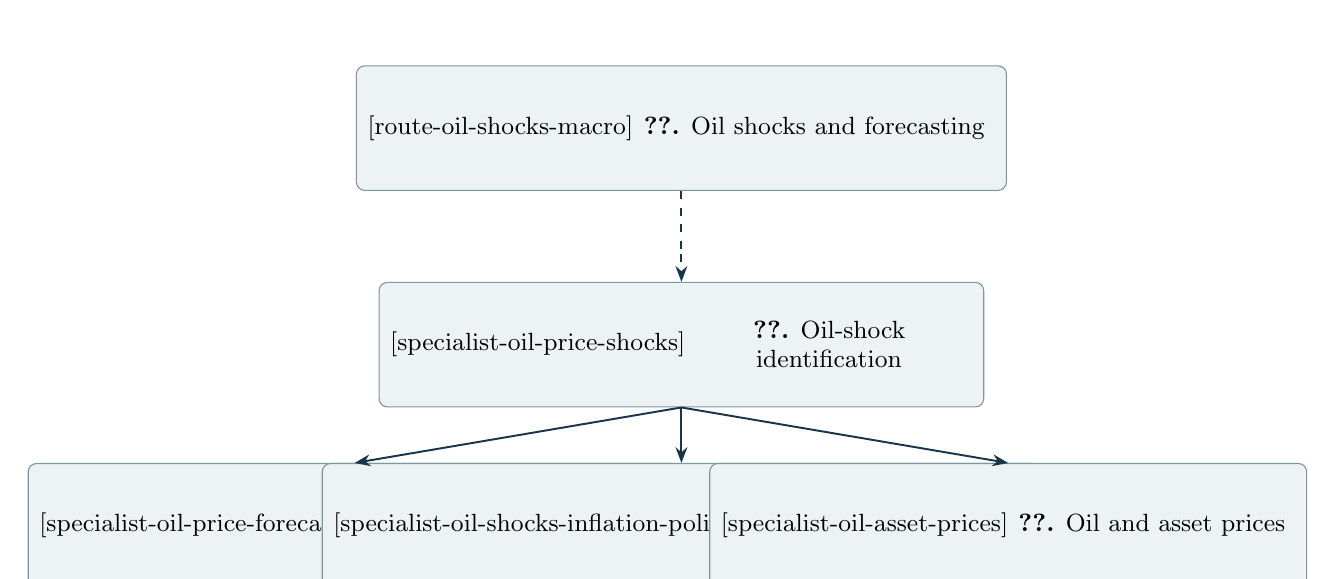
\begin{tikzpicture}[x=1cm,y=1cm]
\node[pathnode] (oil-shocks-macro) at (4.15,0) {\MeasurePathNode{4.6cm}{\textbf{\ref*{route-oil-shocks-macro}.} Oil shocks and forecasting}\hyperref[route-oil-shocks-macro]{\parbox[c][\pathnodeheight][c]{4.6cm}{\centering \textbf{\ref*{route-oil-shocks-macro}.} Oil shocks and forecasting}}};
\node[pathnode] (oil-price-shocks) at (4.15,-2.75) {\MeasurePathNode{3.65cm}{\textbf{\ref*{specialist-oil-price-shocks}.} Oil-shock identification}\hyperref[specialist-oil-price-shocks]{\parbox[c][\pathnodeheight][c]{3.65cm}{\centering \textbf{\ref*{specialist-oil-price-shocks}.} Oil-shock identification}}};
\node[pathnode] (oil-price-forecasting) at (0.00,-5.05) {\MeasurePathNode{3.65cm}{\textbf{\ref*{specialist-oil-price-forecasting}.} Oil-price forecasting}\hyperref[specialist-oil-price-forecasting]{\parbox[c][\pathnodeheight][c]{3.65cm}{\centering \textbf{\ref*{specialist-oil-price-forecasting}.} Oil-price forecasting}}};
\node[pathnode] (oil-shocks-inflation-policy) at (4.15,-5.05) {\MeasurePathNode{3.65cm}{\textbf{\ref*{specialist-oil-shocks-inflation-policy}.} Oil, inflation and policy}\hyperref[specialist-oil-shocks-inflation-policy]{\parbox[c][\pathnodeheight][c]{3.65cm}{\centering \textbf{\ref*{specialist-oil-shocks-inflation-policy}.} Oil, inflation and policy}}};
\node[pathnode] (oil-asset-prices) at (8.30,-5.05) {\MeasurePathNode{3.65cm}{\textbf{\ref*{specialist-oil-asset-prices}.} Oil and asset prices}\hyperref[specialist-oil-asset-prices]{\parbox[c][\pathnodeheight][c]{3.65cm}{\centering \textbf{\ref*{specialist-oil-asset-prices}.} Oil and asset prices}}};
\draw[entryline] (oil-shocks-macro.south) -- (4.15,-1.60);
\draw[entryline] (4.15,-1.60) -- (4.15,-1.60);
\draw[entryarrow] (4.15,-1.60) -- (oil-price-shocks.north);
\draw[patharrow] (oil-price-shocks.south) -- (oil-price-forecasting.north);
\draw[patharrow] (oil-price-shocks.south) -- (oil-shocks-inflation-policy.north);
\draw[patharrow] (oil-price-shocks.south) -- (oil-asset-prices.north);
\end{tikzpicture}\end{center}
\textbf{Overview checkpoint.} A section capstone: complete it after \hyperref[specialist-oil-price-shocks]{\ref*{specialist-oil-price-shocks}}, \hyperref[specialist-oil-price-forecasting]{\ref*{specialist-oil-price-forecasting}} and \hyperref[specialist-oil-shocks-inflation-policy]{\ref*{specialist-oil-shocks-inflation-policy}}.

\textbf{Bring these foundations with you.}\begin{itemize}
\item \hyperref[specialist-time-series-volatility]{Time-series econometrics and volatility forecasting} --- needed by \hyperref[specialist-oil-price-shocks]{Oil-shock identification}.
\item \hyperref[specialist-commodity-premia]{Commodity risk premia: hedging pressure, inventories and the basis} --- needed by \hyperref[specialist-oil-price-forecasting]{Oil-price forecasting}.
\end{itemize}\hyperref[learning-map]{Return to the whole-guide DAG.}
\Needspace{12\baselineskip}
\subsection{Oil supply and demand shocks: structural identification and elasticities}\label{specialist-oil-price-shocks}
\textbf{Specialist pathway.} In \hyperref[route-oil-shocks-macro]{Oil-price shocks, forecasting and the macroeconomy}.

\textbf{Outcome.} Identify oil supply, aggregate demand and oil-specific demand shocks with structural VARs, sign restrictions with elasticity bounds and external instruments, choose and defend a measure of global real activity, and explain why estimated supply elasticities and shock contributions differ across studies.

\textbf{Prerequisites.} Oil-price shocks, forecasting and the macroeconomy overview; time-series econometrics and structural VARs.

\textbf{Review first.} \hyperref[route-oil-shocks-macro]{Oil-price shocks, forecasting and the macroeconomy}; \hyperref[specialist-time-series-volatility]{Time-series econometrics and volatility forecasting}.

\textbf{Required readings, in order}
\begin{enumerate}\raggedright
\Needspace{5\baselineskip}\item \href{institutional_quantitative_finance_reading_list.pdf\#ec-barsky-kilian-2004}{Robert B. Barsky and Lutz Kilian, ``Oil and the Macroeconomy since the 1970s''}\CataloguePage{347}\NoteKey{ec-barsky-kilian-2004}\par \textbf{Foundations.} Rethink causality: oil prices respond to economic conditions as well as drive them.
\Needspace{5\baselineskip}\item \href{institutional_quantitative_finance_reading_list.pdf\#wide-kilian-oil-shocks}{Lutz Kilian, ``Not All Oil Price Shocks Are Alike: Disentangling Demand and Supply Shocks in the Crude Oil Market''}\CataloguePage{347}\NoteKey{wide-kilian-oil-shocks}\par \textbf{Methods.} Identify oil supply and demand shocks.
\Needspace{5\baselineskip}\item \href{institutional_quantitative_finance_reading_list.pdf\#cp-kilian-vega-2011}{Lutz Kilian and Clara Vega, ``Do Energy Prices Respond to U.S. Macroeconomic News? A Test of the Hypothesis of Predetermined Energy Prices''}\CataloguePage{349}\NoteKey{cp-kilian-vega-2011}\par \textbf{Methods.} Test the assumption that oil prices are predetermined with respect to US macroeconomic news.
\Needspace{5\baselineskip}\item \href{institutional_quantitative_finance_reading_list.pdf\#wide-kilian-lutkepohl-svar}{Lutz Kilian and Helmut Lütkepohl, \emph{Structural Vector Autoregressive Analysis}}\CataloguePage{36}\NoteKey{wide-kilian-lutkepohl-svar}\par \textbf{Methods.} Learn structural VAR identification by short-run, sign and external-instrument restrictions.
\Needspace{5\baselineskip}\item \href{institutional_quantitative_finance_reading_list.pdf\#cp-kilian-murphy-2012}{Lutz Kilian and Daniel P. Murphy, ``Why Agnostic Sign Restrictions Are Not Enough: Understanding the Dynamics of Oil Market VAR Models''}\CataloguePage{349}\NoteKey{cp-kilian-murphy-2012}\par \textbf{Methods.} Bound the oil supply elasticity and the real-activity response so that sign restrictions identify the shocks.
\Needspace{5\baselineskip}\item \href{institutional_quantitative_finance_reading_list.pdf\#ec-baumeister-hamilton-2019}{Christiane Baumeister and James D. Hamilton, ``Structural Interpretation of Vector Autoregressions with Incomplete Identification: Revisiting the Role of Oil Supply and Demand Shocks''}\CataloguePage{347}\NoteKey{ec-baumeister-hamilton-2019}\par \textbf{Methods.} Make priors on supply and demand elasticities explicit in a Bayesian structural VAR.
\Needspace{5\baselineskip}\item \href{institutional_quantitative_finance_reading_list.pdf\#ec-caldara-cavallo-iacoviello-2019}{Dario Caldara, Michele Cavallo and Matteo Iacoviello, ``Oil Price Elasticities and Oil Price Fluctuations''}\CataloguePage{347}\NoteKey{ec-caldara-cavallo-iacoviello-2019}\par \textbf{Methods.} Identify oil supply and demand elasticities with country supply disruptions.
\Needspace{5\baselineskip}\item \href{institutional_quantitative_finance_reading_list.pdf\#ec-kanzig-2021}{Diego R. Känzig, ``The Macroeconomic Effects of Oil Supply News: Evidence from OPEC Announcements''}\CataloguePage{347}\NoteKey{ec-kanzig-2021}\par \textbf{Methods.} Use OPEC announcement surprises as an instrument for oil supply news.
\Needspace{5\baselineskip}\item \href{institutional_quantitative_finance_reading_list.pdf\#cp-baumeister-peersman-2013}{Christiane Baumeister and Gert Peersman, ``Time-Varying Effects of Oil Supply Shocks on the US Economy''}\CataloguePage{349}\NoteKey{cp-baumeister-peersman-2013}\par \textbf{Evidence.} See the short-run price elasticity of oil demand fall and the effects of supply shocks change over time.
\Needspace{5\baselineskip}\item \href{institutional_quantitative_finance_reading_list.pdf\#cp-kilian-2022-elasticities}{Lutz Kilian, ``Understanding the estimation of oil demand and oil supply elasticities''}\CataloguePage{349}\NoteKey{cp-kilian-2022-elasticities}\par \textbf{Evidence.} Reconcile conflicting estimates of oil supply and demand elasticities.
\Needspace{5\baselineskip}\item \href{institutional_quantitative_finance_reading_list.pdf\#cp-herrera-rangaraju-2020}{Ana María Herrera and Sandeep Kumar Rangaraju, ``The effect of oil supply shocks on US economic activity: What have we learned?''}\CataloguePage{349}\NoteKey{cp-herrera-rangaraju-2020}\par \textbf{Evidence.} Trace differences in estimated supply-shock effects to identification and specification.
\Needspace{5\baselineskip}\item \href{institutional_quantitative_finance_reading_list.pdf\#ec-kilian-zhou-2018}{Lutz Kilian and Xiaoqing Zhou, ``Modeling Fluctuations in the Global Demand for Commodities''}\CataloguePage{348}\NoteKey{ec-kilian-zhou-2018}\par \textbf{Data.} Compare indices of global real activity for commodity demand.
\Needspace{5\baselineskip}\item \href{institutional_quantitative_finance_reading_list.pdf\#cp-hamilton-2021-activity}{James D. Hamilton, ``Measuring global economic activity''}\CataloguePage{349}\NoteKey{cp-hamilton-2021-activity}\par \textbf{Data.} Check how the freight-rate activity index depends on its normalisation and compare it with world industrial production.
\end{enumerate}
\Needspace{5\baselineskip}\textbf{Checkpoint.} Estimate a monthly VAR in global oil production, a real-activity index, the real oil price and oil inventories from 1974. Identify it three ways: recursively, with sign restrictions and bounds on the impact supply elasticity, and with OPEC announcement surprises as an external instrument. Compare the implied supply elasticities and the decompositions of 2008, 2014--15, 2020 and March 2026, and repeat with Hamilton's industrial-production measure of activity in place of the freight-rate index.

\textbf{Optional branches.} \href{institutional_quantitative_finance_reading_list.pdf\#cp-kilian-2019-activity}{Read Kilian's reply: a coding error, once corrected, leaves the index and results intact.}\BranchPage{349} \href{institutional_quantitative_finance_reading_list.pdf\#cp-baumeister-hamilton-2024}{Survey Bayesian and set-identified VARs and the correct estimation of structural elasticities.}\BranchPage{350} \href{institutional_quantitative_finance_reading_list.pdf\#physical-kilian-murphy-oil-2014}{Add inventories and speculative demand to the oil-market VAR.}\BranchPage{338} \href{institutional_quantitative_finance_reading_list.pdf\#ec-baumeister-kilian-2016b}{Decompose the oil-price collapse of 2014--15.}\BranchPage{348}
\par{\small \hyperref[learning-map]{Learning pathway DAG} \textbar{} \hyperref[route-oil-shocks-macro]{Section overview} \textbar{} \hyperref[map-oil-shocks-macro]{Section DAG}\NoteKey{oil-price-shocks}}
\Needspace{12\baselineskip}
\subsection{Forecasting the real price of oil: futures, VARs and forecast combinations}\label{specialist-oil-price-forecasting}
\textbf{Specialist pathway.} In \hyperref[route-oil-shocks-macro]{Oil-price shocks, forecasting and the macroeconomy}.

\textbf{Outcome.} Build real-time forecasts of the real price of oil from futures, product spreads, VARs and indices of economic conditions, combine them, and evaluate them against the right no-change benchmark and against official forecasts.

\textbf{Prerequisites.} Oil supply and demand shocks (24.1); commodity futures risk premia (23.1); forecast evaluation with real-time data vintages.

\textbf{Review first.} \hyperref[specialist-oil-price-shocks]{Oil supply and demand shocks: structural identification and elasticities}; \hyperref[specialist-commodity-premia]{Commodity risk premia: hedging pressure, inventories and the basis}.

\textbf{Required readings, in order}
\begin{enumerate}\raggedright
\Needspace{5\baselineskip}\item \href{institutional_quantitative_finance_reading_list.pdf\#ec-alquist-kilian-vigfusson-2013}{Ron Alquist, Lutz Kilian and Robert J. Vigfusson, ``Forecasting the Price of Oil''}\CataloguePage{348}\NoteKey{ec-alquist-kilian-vigfusson-2013}\par \textbf{Foundations.} Survey oil-price forecasting methods and how to evaluate them.
\Needspace{5\baselineskip}\item \href{institutional_quantitative_finance_reading_list.pdf\#ec-alquist-kilian-2010}{Ron Alquist and Lutz Kilian, ``What Do We Learn from the Price of Crude Oil Futures?''}\CataloguePage{347}\NoteKey{ec-alquist-kilian-2010}\par \textbf{Evidence.} See that futures prices forecast the spot price no better than a no-change forecast.
\Needspace{5\baselineskip}\item \href{institutional_quantitative_finance_reading_list.pdf\#ec-baumeister-kilian-2012}{Christiane Baumeister and Lutz Kilian, ``Real-Time Forecasts of the Real Price of Oil''}\CataloguePage{348}\NoteKey{ec-baumeister-kilian-2012}\par \textbf{Validation.} Forecast the real price of oil in real time with data vintages.
\Needspace{5\baselineskip}\item \href{institutional_quantitative_finance_reading_list.pdf\#cp-baumeister-kilian-2014}{Christiane Baumeister and Lutz Kilian, ``What Central Bankers Need to Know about Forecasting Oil Prices''}\CataloguePage{350}\NoteKey{cp-baumeister-kilian-2014}\par \textbf{Methods.} Build the quarterly forecasts central banks use from VARs estimated on monthly data.
\Needspace{5\baselineskip}\item \href{institutional_quantitative_finance_reading_list.pdf\#cp-baumeister-kilian-2015}{Christiane Baumeister and Lutz Kilian, ``Forecasting the Real Price of Oil in a Changing World: A Forecast Combination Approach''}\CataloguePage{350}\NoteKey{cp-baumeister-kilian-2015}\par \textbf{Methods.} Combine six real-time models, weighted by recent accuracy, and compare them with EIA forecasts.
\Needspace{5\baselineskip}\item \href{institutional_quantitative_finance_reading_list.pdf\#cp-baumeister-kilian-zhou-2018}{Christiane Baumeister, Lutz Kilian and Xiaoqing Zhou, ``Are Product Spreads Useful for Forecasting Oil Prices? An Empirical Evaluation of the Verleger Hypothesis''}\CataloguePage{350}\NoteKey{cp-baumeister-kilian-zhou-2018}\par \textbf{Evidence.} Test whether refined-product spreads predict crude prices.
\Needspace{5\baselineskip}\item \href{institutional_quantitative_finance_reading_list.pdf\#cp-baumeister-korobilis-lee-2022}{Christiane Baumeister, Dimitris Korobilis and Thomas K. Lee, ``Energy Markets and Global Economic Conditions''}\CataloguePage{350}\NoteKey{cp-baumeister-korobilis-lee-2022}\par \textbf{Data.} Choose an index of global economic conditions for forecasting oil prices and demand.
\Needspace{5\baselineskip}\item \href{institutional_quantitative_finance_reading_list.pdf\#cp-garratt-vahey-zhang-2019}{Anthony Garratt, Shaun P. Vahey and Yunyi Zhang, ``Real-time forecast combinations for the oil price''}\CataloguePage{350}\NoteKey{cp-garratt-vahey-zhang-2019}\par \textbf{Validation.} Replicate the forecast combination, extend it to Brent and fill missing futures prices.
\Needspace{5\baselineskip}\item \href{institutional_quantitative_finance_reading_list.pdf\#cp-ellwanger-snudden-2023}{Reinhard Ellwanger and Stephen Snudden, ``Forecasts of the real price of oil revisited: Do they beat the random walk?''}\CataloguePage{351}\NoteKey{cp-ellwanger-snudden-2023}\par \textbf{Validation.} Benchmark against the end-of-month no-change forecast, not the monthly average.
\Needspace{5\baselineskip}\item \href{institutional_quantitative_finance_reading_list.pdf\#cp-eia-steo-2026}{U.S. Energy Information Administration, Short-Term Energy Outlook, October 2026}\CataloguePage{351}\NoteKey{cp-eia-steo-2026}\par \textbf{Data.} Compare model forecasts with the official monthly outlook and keep the vintage used.
\end{enumerate}
\Needspace{5\baselineskip}\textbf{Checkpoint.} Assemble a real-time monthly dataset since 1990 of the real refiners' acquisition cost and Brent, as monthly averages and end-of-month prices, with the vintages available at each date. Produce 1-, 3-, 12- and 24-month forecasts from the no-change benchmarks, a futures-spread model, a product-spread model, a VAR and a recursively weighted combination. Report MSPE ratios and directional accuracy against each benchmark, with and without 2020 and 2026, and compare the combination with the EIA outlook published in the same month.

\textbf{Optional branches.} \href{institutional_quantitative_finance_reading_list.pdf\#cp-funk-2018}{Extend the combination with more models and check its stability over time.}\BranchPage{350} \href{institutional_quantitative_finance_reading_list.pdf\#ec-chen-rogoff-rossi-2010}{See commodity-currency exchange rates forecast commodity prices.}\BranchPage{348} \href{institutional_quantitative_finance_reading_list.pdf\#sp-chinn-coibion-2014}{Compare the predictive content of futures across energy, metals and agriculture.}\BranchPage{381}
\par{\small \hyperref[learning-map]{Learning pathway DAG} \textbar{} \hyperref[route-oil-shocks-macro]{Section overview} \textbar{} \hyperref[map-oil-shocks-macro]{Section DAG}\NoteKey{oil-price-forecasting}}
\Needspace{12\baselineskip}
\subsection{Oil shocks, inflation and monetary policy}\label{specialist-oil-shocks-inflation-policy}
\textbf{Specialist pathway.} In \hyperref[route-oil-shocks-macro]{Oil-price shocks, forecasting and the macroeconomy}.

\textbf{Outcome.} Trace how oil shocks reach output, consumption, inflation and inflation expectations, test for asymmetry and nonlinearity correctly, and judge the role of monetary policy from the 1970s to the 2021--22 inflation surge.

\textbf{Prerequisites.} Oil supply and demand shocks (24.1); New Keynesian models and monetary policy rules at an introductory level.

\textbf{Review first.} \hyperref[specialist-oil-price-shocks]{Oil supply and demand shocks: structural identification and elasticities}.

\textbf{Required readings, in order}
\begin{enumerate}\raggedright
\Needspace{5\baselineskip}\item \href{institutional_quantitative_finance_reading_list.pdf\#ec-hamilton-1983}{James D. Hamilton, ``Oil and the Macroeconomy since World War II''}\CataloguePage{351}\NoteKey{ec-hamilton-1983}\par \textbf{Foundations.} See that oil-price increases preceded most postwar US recessions.
\Needspace{5\baselineskip}\item \href{institutional_quantitative_finance_reading_list.pdf\#cp-hooker-1996}{Mark A. Hooker, ``What happened to the oil price-macroeconomy relationship?''}\CataloguePage{351}\NoteKey{cp-hooker-1996}\par \textbf{Evidence.} See the oil--macroeconomy relationship break down in data after 1973.
\Needspace{5\baselineskip}\item \href{institutional_quantitative_finance_reading_list.pdf\#cp-hamilton-1996}{James D. Hamilton, ``This is what happened to the oil price-macroeconomy relationship''}\CataloguePage{351}\NoteKey{cp-hamilton-1996}\par \textbf{Evidence.} See the net increase over the previous year restore the link between oil shocks and recessions.
\Needspace{5\baselineskip}\item \href{institutional_quantitative_finance_reading_list.pdf\#ec-hamilton-2003}{James D. Hamilton, ``What Is an Oil Shock?''}\CataloguePage{351}\NoteKey{ec-hamilton-2003}\par \textbf{Methods.} Define an oil shock as a net price increase and model the nonlinearity.
\Needspace{5\baselineskip}\item \href{institutional_quantitative_finance_reading_list.pdf\#cp-kilian-vigfusson-2011}{Lutz Kilian and Robert J. Vigfusson, ``Are the responses of the U.S. economy asymmetric in energy price increases and decreases?''}\CataloguePage{352}\NoteKey{cp-kilian-vigfusson-2011}\par \textbf{Methods.} See why censored oil-price VARs overstate asymmetry and how to test for it correctly.
\Needspace{5\baselineskip}\item \href{institutional_quantitative_finance_reading_list.pdf\#cp-edelstein-kilian-2009}{Paul Edelstein and Lutz Kilian, ``How sensitive are consumer expenditures to retail energy prices?''}\CataloguePage{352}\NoteKey{cp-edelstein-kilian-2009}\par \textbf{Evidence.} Measure how energy-price shocks reduce consumer spending.
\Needspace{5\baselineskip}\item \href{institutional_quantitative_finance_reading_list.pdf\#cp-bgw-1997}{Ben S. Bernanke, Mark Gertler and Mark Watson, ``Systematic Monetary Policy and the Effects of Oil Price Shocks''}\CataloguePage{352}\NoteKey{cp-bgw-1997}\par \textbf{Evidence.} See the argument that systematic monetary tightening caused much of the output loss after oil shocks.
\Needspace{5\baselineskip}\item \href{institutional_quantitative_finance_reading_list.pdf\#cp-hamilton-herrera-2004}{James D. Hamilton and Ana María Herrera, ``Oil Shocks and Aggregate Macroeconomic Behavior: The Role of Monetary Policy: A Comment''}\CataloguePage{352}\NoteKey{cp-hamilton-herrera-2004}\par \textbf{Evidence.} Weigh the critique of that counterfactual: feasible policy and longer lags.
\Needspace{5\baselineskip}\item \href{institutional_quantitative_finance_reading_list.pdf\#cp-kilian-lewis-2011}{Lutz Kilian and Logan T. Lewis, ``Does the Fed Respond to Oil Price Shocks?''}\CataloguePage{352}\NoteKey{cp-kilian-lewis-2011}\par \textbf{Evidence.} Test the Federal Reserve's response to oil shocks with the oil price treated as endogenous.
\Needspace{5\baselineskip}\item \href{institutional_quantitative_finance_reading_list.pdf\#cp-blanchard-gali-2010}{Olivier J. Blanchard and Jordi Galí, ``The Macroeconomic Effects of Oil Price Shocks: Why Are the 2000s so Different from the 1970s?''}\CataloguePage{352}\NoteKey{cp-blanchard-gali-2010}\par \textbf{Evidence.} Explain why the oil shocks of the 2000s did less damage than those of the 1970s.
\Needspace{5\baselineskip}\item \href{institutional_quantitative_finance_reading_list.pdf\#ec-hamilton-2009}{James D. Hamilton, ``Causes and Consequences of the Oil Shock of 2007--08''}\CataloguePage{351}\NoteKey{ec-hamilton-2009}\par \textbf{Evidence.} Explain the 2007--08 price spike and its macroeconomic effects.
\Needspace{5\baselineskip}\item \href{institutional_quantitative_finance_reading_list.pdf\#cp-coibion-gorodnichenko-2015}{Olivier Coibion and Yuriy Gorodnichenko, ``Is the Phillips Curve Alive and Well after All? Inflation Expectations and the Missing Disinflation''}\CataloguePage{352}\NoteKey{cp-coibion-gorodnichenko-2015}\par \textbf{Evidence.} Link the missing disinflation after 2009 to oil-driven household inflation expectations.
\Needspace{5\baselineskip}\item \href{institutional_quantitative_finance_reading_list.pdf\#cp-kilian-zhou-2022}{Lutz Kilian and Xiaoqing Zhou, ``Oil prices, gasoline prices, and inflation expectations''}\CataloguePage{353}\NoteKey{cp-kilian-zhou-2022}\par \textbf{Evidence.} Quantify how gasoline-price shocks move household inflation expectations.
\Needspace{5\baselineskip}\item \href{institutional_quantitative_finance_reading_list.pdf\#cp-gagliardone-gertler-2026}{Luca Gagliardone and Mark Gertler, ``Oil Prices, Monetary Policy, and Inflation Surges''}\CataloguePage{353}\NoteKey{cp-gagliardone-gertler-2026}\par \textbf{Evidence.} Weigh oil shocks against accommodative policy in the 2021--22 inflation surge.
\end{enumerate}
\Needspace{5\baselineskip}\textbf{Checkpoint.} Using the shocks identified in 24.1, estimate the responses of US headline and core CPI, household one-year inflation expectations, real consumption and industrial production. Test symmetry with the Kilian--Vigfusson procedure and compare a censored net-oil-price-increase model. Rerun a Bernanke--Gertler--Watson counterfactual that holds the federal funds rate on its pre-shock path, at their lag length and at the longer one Hamilton and Herrera prefer, and compare 1973--74, 1979--80, 2007--08, 2021--22 and 2026.

\textbf{Optional branches.} \href{institutional_quantitative_finance_reading_list.pdf\#cp-wong-2015}{Check whether inflation expectations pass oil shocks through to inflation.}\BranchPage{353} \href{institutional_quantitative_finance_reading_list.pdf\#cp-elder-serletis-2010}{Add oil-price uncertainty and its effect on investment and output.}\BranchPage{353}
\par{\small \hyperref[learning-map]{Learning pathway DAG} \textbar{} \hyperref[route-oil-shocks-macro]{Section overview} \textbar{} \hyperref[map-oil-shocks-macro]{Section DAG}\NoteKey{oil-shocks-inflation-policy}}
\Needspace{12\baselineskip}
\subsection{Oil shocks and asset prices: equities, oil risk factors and currencies}\label{specialist-oil-asset-prices}
\textbf{Specialist pathway.} In \hyperref[route-oil-shocks-macro]{Oil-price shocks, forecasting and the macroeconomy}.

\textbf{Outcome.} Explain how oil shocks move stock prices through cash flows and discount rates, price oil risk and oil-volatility risk in the cross-section of stocks, judge whether oil predicts stock returns, and measure links between oil and commodity currencies.

\textbf{Prerequisites.} Oil supply and demand shocks (24.1); cross-sectional asset pricing; currency risk premia for the exchange-rate readings.

\textbf{Review first.} \hyperref[specialist-oil-price-shocks]{Oil supply and demand shocks: structural identification and elasticities}.

\textbf{Required readings, in order}
\begin{enumerate}\raggedright
\Needspace{5\baselineskip}\item \href{institutional_quantitative_finance_reading_list.pdf\#cp-jones-kaul-1996}{Charles M. Jones and Gautam Kaul, ``Oil and the Stock Markets''}\CataloguePage{354}\NoteKey{cp-jones-kaul-1996}\par \textbf{Evidence.} Test whether stock reactions to oil shocks match changes in real cash flows.
\Needspace{5\baselineskip}\item \href{institutional_quantitative_finance_reading_list.pdf\#ec-kilian-park-2009}{Lutz Kilian and Cheolbeom Park, ``The Impact of Oil Price Shocks on the U.S. Stock Market''}\CataloguePage{353}\NoteKey{ec-kilian-park-2009}\par \textbf{Evidence.} Trace stock-market responses to oil supply and demand shocks.
\Needspace{5\baselineskip}\item \href{institutional_quantitative_finance_reading_list.pdf\#ec-ready-2018}{Robert C. Ready, ``Oil Prices and the Stock Market''}\CataloguePage{353}\NoteKey{ec-ready-2018}\par \textbf{Evidence.} Separate oil supply from demand shocks with oil-producer equity returns.
\Needspace{5\baselineskip}\item \href{institutional_quantitative_finance_reading_list.pdf\#ec-driesprong-2008}{Gerben Driesprong, Ben Jacobsen and Benjamin Maat, ``Striking Oil: Another Puzzle?''}\CataloguePage{353}\NoteKey{ec-driesprong-2008}\par \textbf{Evidence.} Test whether oil-price changes predict stock returns.
\Needspace{5\baselineskip}\item \href{institutional_quantitative_finance_reading_list.pdf\#cp-chiang-hughen-sagi-2015}{I-Hsuan Ethan Chiang, W. Keener Hughen and Jacob S. Sagi, ``Estimating Oil Risk Factors Using Information from Equity and Derivatives Markets''}\CataloguePage{354}\NoteKey{cp-chiang-hughen-sagi-2015}\par \textbf{Evidence.} Estimate latent oil risk factors from derivatives and equities and price them in non-oil stocks.
\Needspace{5\baselineskip}\item \href{institutional_quantitative_finance_reading_list.pdf\#cp-christoffersen-pan-2018}{Peter Christoffersen and Xuhui (Nick) Pan, ``Oil volatility risk and expected stock returns''}\CataloguePage{354}\NoteKey{cp-christoffersen-pan-2018}\par \textbf{Evidence.} Price oil-volatility risk in the cross-section of stocks after financialisation.
\Needspace{5\baselineskip}\item \href{institutional_quantitative_finance_reading_list.pdf\#cp-datta-2021}{Deepa D. Datta, Benjamin K. Johannsen, Hannah Kwon and Robert J. Vigfusson, ``Oil, Equities, and the Zero Lower Bound''}\CataloguePage{354}\NoteKey{cp-datta-2021}\par \textbf{Evidence.} See oil and equity returns comove more at the zero lower bound.
\Needspace{5\baselineskip}\item \href{institutional_quantitative_finance_reading_list.pdf\#cp-ferraro-rogoff-rossi-2015}{Domenico Ferraro, Kenneth Rogoff and Barbara Rossi, ``Can oil prices forecast exchange rates? An empirical analysis of the relationship between commodity prices and exchange rates''}\CataloguePage{354}\NoteKey{cp-ferraro-rogoff-rossi-2015}\par \textbf{Evidence.} Relate daily oil-price changes to commodity-currency exchange rates.
\Needspace{5\baselineskip}\item \href{institutional_quantitative_finance_reading_list.pdf\#cur-ready-roussanov-ward-2017}{Robert Ready, Nikolai Roussanov and Colin Ward, ``Commodity Trade and the Carry Trade: A Tale of Two Countries''}\CataloguePage{281}\NoteKey{cur-ready-roussanov-ward-2017}\par \textbf{Evidence.} See why commodity exporters carry high interest rates and currency risk premia.
\end{enumerate}
\Needspace{5\baselineskip}\textbf{Checkpoint.} Using Ready's decomposition and the structural shocks from 24.1, regress monthly US market, industry and oil-producer returns on supply and demand shocks since 1986. Sort stocks on their beta to changes in oil implied volatility and report the return spread before and after 2005, test whether lagged oil-price changes predict market returns out of sample, and estimate rolling oil--equity correlations around 2008--15 and 2020--21. Finish with daily regressions of the Canadian dollar and the Norwegian krone on contemporaneous and lagged oil-price changes.

\textbf{Optional branches.} \href{institutional_quantitative_finance_reading_list.pdf\#cp-narayan-sharma-2011}{See oil effects on firm returns vary by sector, lag and firm size.}\BranchPage{354} \href{institutional_quantitative_finance_reading_list.pdf\#sp-chen-rogoff-2003}{Read the original evidence on commodity currencies.}\BranchPage{381} \href{institutional_quantitative_finance_reading_list.pdf\#cp-buyuksahin-robe-2014}{See speculators' positions predict commodity--equity correlation.}\BranchPage{341}
\par{\small \hyperref[learning-map]{Learning pathway DAG} \textbar{} \hyperref[route-oil-shocks-macro]{Section overview} \textbar{} \hyperref[map-oil-shocks-macro]{Section DAG}\NoteKey{oil-asset-prices}}
\clearpage
\section{Gas and power markets: hubs, storage, networks and market design}\label{route-power-gas-environmental}
\label{route-20}
\textbf{Learning sequence.} Start with gas hub pricing and market integration (25.1), then value storage, transport and LNG options (25.2). Power networks and transmission rights (25.3) come before market design (25.4), renewable value (25.5), price modelling and forecasting (25.6) and short-term markets and flexibility (25.7). Environmental markets follow in the next section.

\textbf{Section goals.} Across its pathways, this section teaches you to:
\begin{itemize}[leftmargin=1.4em,itemsep=0pt,topsep=1pt]
\item test gas-market integration and oil indexation, and analyse supply shocks (\hyperref[specialist-gas-hub-pricing]{\ref*{specialist-gas-hub-pricing}})
\item value gas storage, transport and LNG options (\hyperref[specialist-physical-lng]{\ref*{specialist-physical-lng}})
\item explain nodal prices, congestion, PPA and storage cash flows (\hyperref[specialist-power-ftr]{\ref*{specialist-power-ftr}})
\item judge electricity market designs, capacity payments and market power (\hyperref[specialist-power-market-design]{\ref*{specialist-power-market-design}})
\item measure renewable value and price PPA risks (\hyperref[specialist-renewables-ppa-value]{\ref*{specialist-renewables-ppa-value}})
\item model and forecast electricity prices (\hyperref[specialist-power-price-forecasting]{\ref*{specialist-power-price-forecasting}})
\item trade intraday and balancing markets and value storage arbitrage (\hyperref[specialist-power-short-term-flexibility]{\ref*{specialist-power-short-term-flexibility}})
\end{itemize}
\textbf{Overview outcome.} Value a storage or dispatch asset's cash flows in a normal and a network-constrained week, and show how a data-release lag or a delivery-rule change alters its hedge.

\textbf{Prerequisites.} Commodity futures: storage, curves, hedging and options; constrained optimisation and time-series forecasting.

\textbf{Review first.} \hyperref[route-energy-commodities]{Commodity futures: storage, curves, hedging and options}.

\textbf{Required readings, in order}
\begin{enumerate}\raggedright
\Needspace{5\baselineskip}\item \href{institutional_quantitative_finance_reading_list.pdf\#physical-secomandi-storage-2010}{Nicola Secomandi, Optimal Commodity Trading with a Capacitated Storage Asset}\CataloguePage{319}\NoteKey{physical-secomandi-storage-2010}\par Value the operating option in a capacity-constrained storage asset.
\Needspace{5\baselineskip}\item \href{institutional_quantitative_finance_reading_list.pdf\#physical-eia-gas-storage-2026}{U.S. Energy Information Administration, Weekly Natural Gas Storage Report; EIA storage, price and LNG market supplement}\CataloguePage{320}\NoteKey{physical-eia-gas-storage-2026}\par Use dated public inventory data while preserving release times and revisions.
\Needspace{5\baselineskip}\item \href{institutional_quantitative_finance_reading_list.pdf\#exp-bessembinder-lemmon-power-forward}{Hendrik Bessembinder and Michael L. Lemmon, Equilibrium Pricing and Optimal Hedging in Electricity Forward Markets}\CataloguePage{328}\NoteKey{exp-bessembinder-lemmon-power-forward}\par See why nonstorability and load risk change electricity forward pricing.
\Needspace{5\baselineskip}\item \href{institutional_quantitative_finance_reading_list.pdf\#depth-ferc-nodal-ancillary}{Federal Energy Regulatory Commission, Energy Markets; Ancillary Services}\CataloguePage{358}\NoteKey{depth-ferc-nodal-ancillary}\par Map power value to location, dispatch and ancillary-service market rules.
\Needspace{5\baselineskip}\item \href{institutional_quantitative_finance_reading_list.pdf\#exp-uniejewski-ziel-probabilistic-power}{Bartosz Uniejewski and Florian Ziel, The Role of Probabilistic Load and Renewable Prediction in Enhancing Day-Ahead Electricity Price Forecasts}\CataloguePage{328}\NoteKey{exp-uniejewski-ziel-probabilistic-power}\par Test how probabilistic load and renewable forecasts improve day-ahead price forecasts; a profitable hedge needs a separate evaluation.
\end{enumerate}
\Needspace{5\baselineskip}\textbf{Checkpoint.} Choose one storage or dispatch asset and specify location, capacity, losses, delivery windows and hedge contracts. Calculate cash flows across a normal and constrained week, then show how a data-release lag or delivery-rule change alters the hedge.

\textbf{Optional branches.} \href{institutional_quantitative_finance_reading_list.pdf\#section.14.11}{Browse gas hub pricing, market integration and supply-shock studies.}\BranchPage{354}
\par\textbf{Continue in this section.} \hyperref[specialist-gas-hub-pricing]{Natural gas markets: hub pricing, oil indexation, market integration and supply shocks}; \hyperref[specialist-physical-lng]{Natural gas storage, transport and LNG optionality}; \hyperref[specialist-power-ftr]{Power, storage and transmission rights}; \hyperref[specialist-power-market-design]{Electricity market design: scarcity pricing, capacity and market power}; \hyperref[specialist-renewables-ppa-value]{Renewable value, cannibalisation and PPA risk}; \hyperref[specialist-power-price-forecasting]{Electricity price modelling and forecasting}; \hyperref[specialist-power-short-term-flexibility]{Short-term power markets: intraday trading, balancing, negative prices and storage arbitrage}.
\par{\small \hyperref[learning-map]{Learning pathway DAG} \textbar{} \hyperref[map-power-gas-environmental]{Section DAG}\NoteKey{power-gas-environmental}}
\clearpage
\subsection*{Gas and power markets: hubs, storage, networks and market design: pathway DAG}\phantomsection\label{map-power-gas-environmental}
\addcontentsline{toc}{subsection}{Gas and power markets: hubs, storage, networks and market design: pathway DAG}
Start with the section overview's readings, for orientation. Solid arrows show prerequisites within this section. Dashed connectors identify entry points with no further prerequisite in this section; the linked foundations below still apply. Follow the arrows for dependencies and the subsection numbers for reading order. Every node is clickable.
\begin{center}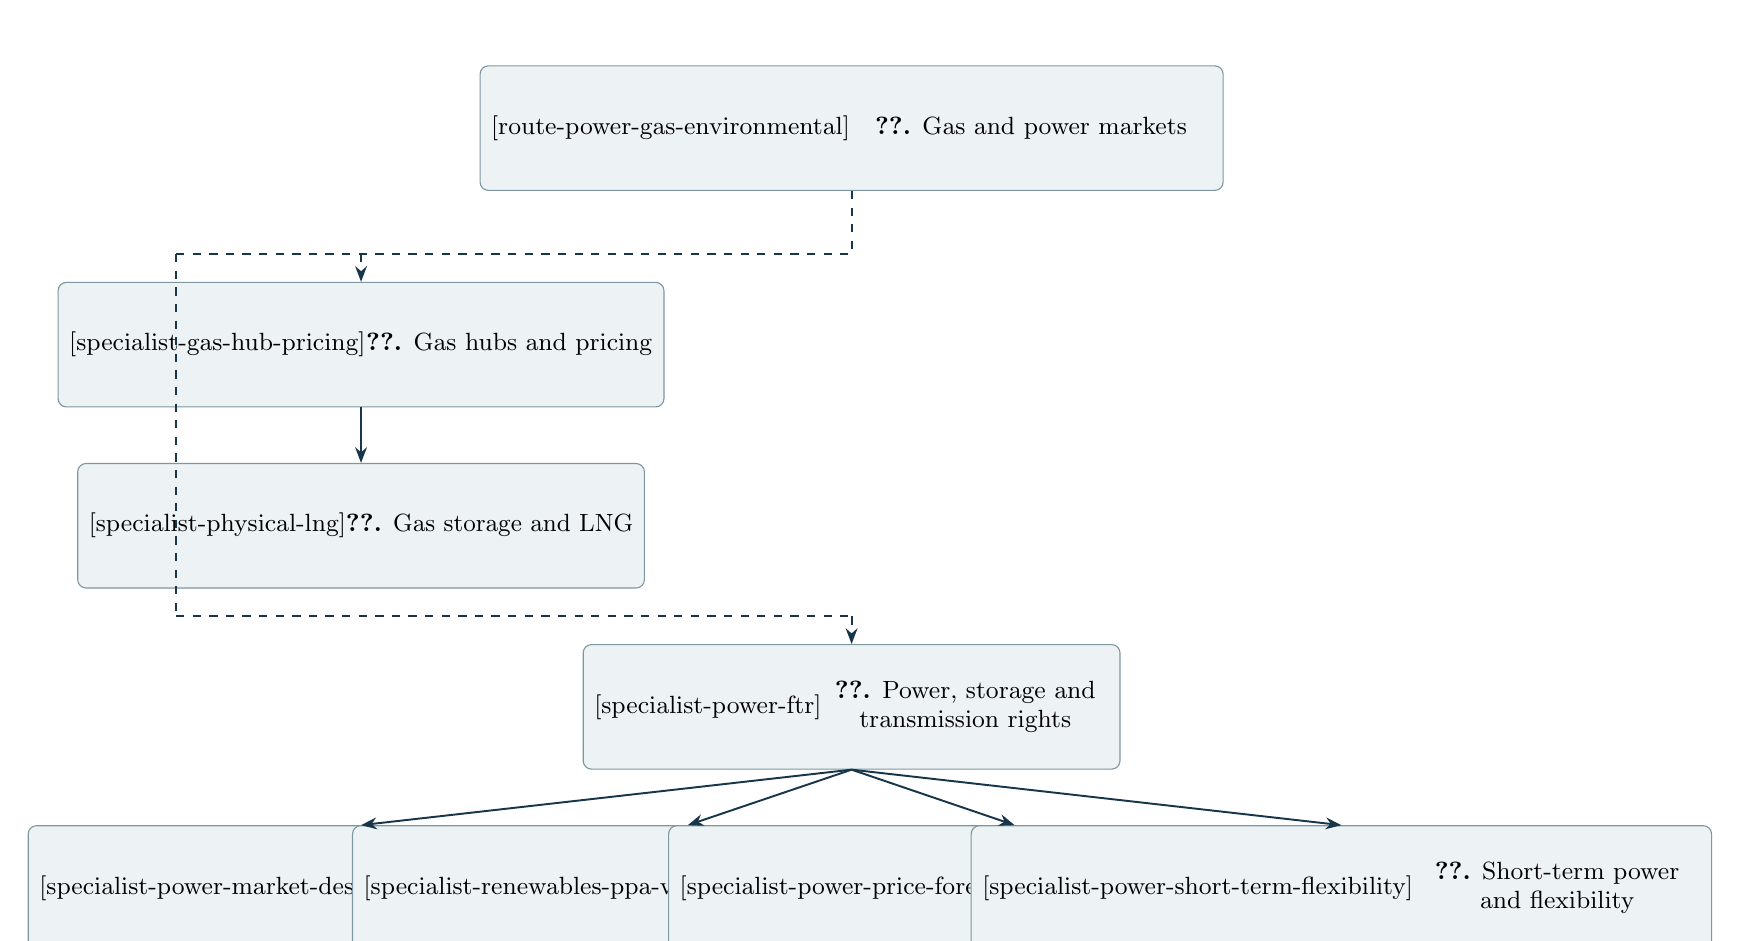
\begin{tikzpicture}[x=1cm,y=1cm]
\node[pathnode] (power-gas-environmental) at (6.23,0) {\MeasurePathNode{4.6cm}{\textbf{\ref*{route-power-gas-environmental}.} Gas and power markets}\hyperref[route-power-gas-environmental]{\parbox[c][\pathnodeheight][c]{4.6cm}{\centering \textbf{\ref*{route-power-gas-environmental}.} Gas and power markets}}};
\node[pathnode] (gas-hub-pricing) at (0.00,-2.75) {\MeasurePathNode{3.65cm}{\textbf{\ref*{specialist-gas-hub-pricing}.} Gas hubs and pricing}\hyperref[specialist-gas-hub-pricing]{\parbox[c][\pathnodeheight][c]{3.65cm}{\centering \textbf{\ref*{specialist-gas-hub-pricing}.} Gas hubs and pricing}}};
\node[pathnode] (physical-lng) at (0.00,-5.05) {\MeasurePathNode{3.65cm}{\textbf{\ref*{specialist-physical-lng}.} Gas storage and LNG}\hyperref[specialist-physical-lng]{\parbox[c][\pathnodeheight][c]{3.65cm}{\centering \textbf{\ref*{specialist-physical-lng}.} Gas storage and LNG}}};
\node[pathnode] (power-ftr) at (6.23,-7.35) {\MeasurePathNode{3.65cm}{\textbf{\ref*{specialist-power-ftr}.} Power, storage and transmission rights}\hyperref[specialist-power-ftr]{\parbox[c][\pathnodeheight][c]{3.65cm}{\centering \textbf{\ref*{specialist-power-ftr}.} Power, storage and transmission rights}}};
\node[pathnode] (power-market-design) at (0.00,-9.65) {\MeasurePathNode{3.65cm}{\textbf{\ref*{specialist-power-market-design}.} Power market design}\hyperref[specialist-power-market-design]{\parbox[c][\pathnodeheight][c]{3.65cm}{\centering \textbf{\ref*{specialist-power-market-design}.} Power market design}}};
\node[pathnode] (renewables-ppa-value) at (4.15,-9.65) {\MeasurePathNode{3.65cm}{\textbf{\ref*{specialist-renewables-ppa-value}.} Renewable value and PPAs}\hyperref[specialist-renewables-ppa-value]{\parbox[c][\pathnodeheight][c]{3.65cm}{\centering \textbf{\ref*{specialist-renewables-ppa-value}.} Renewable value and PPAs}}};
\node[pathnode] (power-price-forecasting) at (8.30,-9.65) {\MeasurePathNode{3.65cm}{\textbf{\ref*{specialist-power-price-forecasting}.} Power price forecasting}\hyperref[specialist-power-price-forecasting]{\parbox[c][\pathnodeheight][c]{3.65cm}{\centering \textbf{\ref*{specialist-power-price-forecasting}.} Power price forecasting}}};
\node[pathnode] (power-short-term-flexibility) at (12.45,-9.65) {\MeasurePathNode{3.65cm}{\textbf{\ref*{specialist-power-short-term-flexibility}.} Short-term power and flexibility}\hyperref[specialist-power-short-term-flexibility]{\parbox[c][\pathnodeheight][c]{3.65cm}{\centering \textbf{\ref*{specialist-power-short-term-flexibility}.} Short-term power and flexibility}}};
\draw[entryline] (power-gas-environmental.south) -- (6.23,-1.60);
\draw[entryline] (-2.35,-1.60) -- (-2.35,-6.20);
\draw[entryline] (-2.35,-1.60) -- (6.23,-1.60);
\draw[entryarrow] (0.00,-1.60) -- (gas-hub-pricing.north);
\draw[entryline] (-2.35,-6.20) -- (6.23,-6.20);
\draw[entryarrow] (6.23,-6.20) -- (power-ftr.north);
\draw[patharrow] (gas-hub-pricing.south) -- (physical-lng.north);
\draw[patharrow] (power-ftr.south) -- (power-market-design.north);
\draw[patharrow] (power-ftr.south) -- (renewables-ppa-value.north);
\draw[patharrow] (power-ftr.south) -- (power-price-forecasting.north);
\draw[patharrow] (power-ftr.south) -- (power-short-term-flexibility.north);
\end{tikzpicture}\end{center}
\textbf{Bring these foundations with you.}\begin{itemize}
\item \hyperref[specialist-time-series-volatility]{Time-series econometrics and volatility forecasting} --- needed by \hyperref[specialist-power-price-forecasting]{Power price forecasting}.
\end{itemize}\hyperref[learning-map]{Return to the whole-guide DAG.}
\Needspace{12\baselineskip}
\subsection{Natural gas markets: hub pricing, oil indexation, market integration and supply shocks}\label{specialist-gas-hub-pricing}
\textbf{Specialist pathway.} In \hyperref[route-power-gas-environmental]{Gas and power markets: hubs, storage, networks and market design}.

\textbf{Outcome.} Explain how open access and liberalisation created traded gas hubs, test whether regional and international gas prices are integrated or tied to oil, and analyse how supply shocks such as shale gas and the 2022 loss of Russian supply moved prices, quantities and welfare.

\textbf{Prerequisites.} Gas and power markets overview; cointegration and time-series econometrics. Spatial arbitrage and market integration (21.2) helps.

\textbf{Review first.} \hyperref[route-power-gas-environmental]{Gas and power markets: hubs, storage, networks and market design}.

\textbf{Required readings, in order}
\begin{enumerate}\raggedright
\Needspace{5\baselineskip}\item \href{institutional_quantitative_finance_reading_list.pdf\#gp-joskow-2013}{Paul L Joskow, ``Natural Gas: From Shortages to Abundance in the United States''}\CataloguePage{355}\NoteKey{gp-joskow-2013}\par \textbf{Foundations.} Trace US wellhead and pipeline regulation, open access and the shale boom behind hub pricing.
\Needspace{5\baselineskip}\item \href{institutional_quantitative_finance_reading_list.pdf\#gp-devany-walls-1993}{Arthur De Vany and W. David Walls, ``Pipeline Access and Market Integration in the Natural Gas Industry: Evidence from Cointegration Tests''}\CataloguePage{355}\NoteKey{gp-devany-walls-1993}\par \textbf{Evidence.} See open pipeline access integrate US field markets between 1987 and 1991.
\Needspace{5\baselineskip}\item \href{institutional_quantitative_finance_reading_list.pdf\#gp-cuddington-wang-2006}{John T. Cuddington and Zhongmin Wang, ``Assessing the Degree of Spot Market Integration for U.S. Natural Gas: Evidence from Daily Price Data''}\CataloguePage{355}\NoteKey{gp-cuddington-wang-2006}\par \textbf{Evidence.} Map an integrated East and Central US market and a segmented West.
\Needspace{5\baselineskip}\item \href{institutional_quantitative_finance_reading_list.pdf\#ec-brown-yucel-2008}{Stephen P. A. Brown and Mine K. Yücel, ``What Drives Natural Gas Prices?''}\CataloguePage{355}\NoteKey{ec-brown-yucel-2008}\par \textbf{Evidence.} Relate US gas prices to oil, weather and storage.
\Needspace{5\baselineskip}\item \href{institutional_quantitative_finance_reading_list.pdf\#gp-hausman-kellogg-2015}{Catherine Hausman and Ryan Kellogg, ``Welfare and Distributional Implications of Shale Gas''}\CataloguePage{355}\NoteKey{gp-hausman-kellogg-2015}\par \textbf{Evidence.} Estimate the price and welfare effects of shale gas by sector and region.
\Needspace{5\baselineskip}\item \href{institutional_quantitative_finance_reading_list.pdf\#ec-hartley-medlock-rosthal-2008}{Peter R. Hartley, Kenneth B. Medlock III and Jennifer E. Rosthal, ``The Relationship of Natural Gas to Oil Prices''}\CataloguePage{354}\NoteKey{ec-hartley-medlock-rosthal-2008}\par \textbf{Evidence.} Model the long-run link between natural gas and oil prices.
\Needspace{5\baselineskip}\item \href{institutional_quantitative_finance_reading_list.pdf\#gp-ramberg-parsons-2012}{David J. Ramberg and John E. Parsons, ``The Weak Tie Between Natural Gas and Oil Prices''}\CataloguePage{355}\NoteKey{gp-ramberg-parsons-2012}\par \textbf{Evidence.} See why the oil--gas cointegrating relation is weak and unstable.
\Needspace{5\baselineskip}\item \href{institutional_quantitative_finance_reading_list.pdf\#ec-erdos-2012}{Péter Erdős, ``Have Oil and Gas Prices Got Separated?''}\CataloguePage{355}\NoteKey{ec-erdos-2012}\par \textbf{Evidence.} See US and European gas prices decouple from oil after 2009.
\Needspace{5\baselineskip}\item \href{institutional_quantitative_finance_reading_list.pdf\#gp-growitsch-2015}{Christian Growitsch, Rabindra Nepal and Marcus Stronzik, ``Price Convergence and Information Efficiency in German Natural Gas Markets''}\CataloguePage{356}\NoteKey{gp-growitsch-2015}\par \textbf{Evidence.} Test price convergence between German hubs and the Dutch market after entry--exit reform.
\Needspace{5\baselineskip}\item \href{institutional_quantitative_finance_reading_list.pdf\#gp-hulshof-2016}{Daan Hulshof, Jan-Pieter van der Maat and Machiel Mulder, ``Market fundamentals, competition and natural-gas prices''}\CataloguePage{356}\NoteKey{gp-hulshof-2016}\par \textbf{Evidence.} Explain TTF day-ahead prices by fundamentals rather than oil indexation.
\Needspace{5\baselineskip}\item \href{institutional_quantitative_finance_reading_list.pdf\#gp-neumann-2009}{Anne Neumann, ``Linking Natural Gas Markets - Is LNG Doing its Job?''}\CataloguePage{356}\NoteKey{gp-neumann-2009}\par \textbf{Evidence.} Measure transatlantic price convergence as LNG trade grew.
\Needspace{5\baselineskip}\item \href{institutional_quantitative_finance_reading_list.pdf\#gp-li-joyeux-ripple-2014}{Raymond Li, Roselyne Joyeux and Ronald D. Ripple, ``International Natural Gas Market Integration''}\CataloguePage{356}\NoteKey{gp-li-joyeux-ripple-2014}\par \textbf{Evidence.} Test integration of North American, European and Asian prices and the role of oil-indexed contracts.
\Needspace{5\baselineskip}\item \href{institutional_quantitative_finance_reading_list.pdf\#gp-ruhnau-2023}{Oliver Ruhnau, Clemens Stiewe, Jarusch Muessel and Lion Hirth, ``Natural gas savings in Germany during the 2022 energy crisis''}\CataloguePage{356}\NoteKey{gp-ruhnau-2023}\par \textbf{Evidence.} Estimate how German consumers cut gas use during the 2021--22 crisis.
\Needspace{5\baselineskip}\item \href{institutional_quantitative_finance_reading_list.pdf\#gp-moll-2023}{Benjamin Moll, Moritz Schularick and Georg Zachmann, ``The Power of Substitution: The Great German Gas Debate in Retrospect''}\CataloguePage{356}\NoteKey{gp-moll-2023}\par \textbf{Evidence.} Assess Germany's adjustment to the 2022 loss of Russian gas through imports and substitution.
\Needspace{5\baselineskip}\item \href{institutional_quantitative_finance_reading_list.pdf\#gp-eu-russian-gas-2026}{European Commission, Directorate-General for Energy, REPowerEU gas regulation: Regulation (EU) 2026/261 phasing out Russian natural gas imports; Legislative Observatory summary, 2025/0180(COD)}\CataloguePage{357}\NoteKey{gp-eu-russian-gas-2026}\par \textbf{Regulation.} Read the 2026 EU ban on Russian pipeline gas and LNG, its deadlines and its TTF-linked penalties.
\end{enumerate}
\Needspace{5\baselineskip}\textbf{Checkpoint.} Assemble daily Henry Hub, TTF and NBP prices, Japan's monthly LNG import price and Brent since 2010. Test pairwise cointegration in rolling windows with a time-varying convergence measure, and date when TTF decoupled from oil and from NBP. Estimate how German gas demand responded in 2022 against a temperature-adjusted baseline, then list the contracts and routes the 2026 Russian gas ban removes and how it values penalties.

\textbf{Optional branches.} \href{institutional_quantitative_finance_reading_list.pdf\#gp-newell-prest-vissing-2019}{Measure how fast shale-gas drilling and supply respond to prices.}\BranchPage{356} \href{institutional_quantitative_finance_reading_list.pdf\#gp-bachmann-2024}{Compare the 2022 ex ante estimate of a Russian energy cut-off with the outcome.}\BranchPage{357} \href{institutional_quantitative_finance_reading_list.pdf\#gp-asche-2006}{Test whether liberalised UK gas prices decoupled from oil and electricity.}\BranchPage{357} \href{institutional_quantitative_finance_reading_list.pdf\#gp-emery-liu-2002}{Study the cointegration of electricity and gas futures and the spark spread.}\BranchPage{357} \href{institutional_quantitative_finance_reading_list.pdf\#sp-hubbard-weiner-1991}{See efficient contracting and market power in the US gas industry.}\BranchPage{377} \href{institutional_quantitative_finance_reading_list.pdf\#sp-oliver-mason-finnoff-2014}{Relate pipeline congestion to gas basis differentials.}\BranchPage{379}
\par{\small \hyperref[learning-map]{Learning pathway DAG} \textbar{} \hyperref[route-power-gas-environmental]{Section overview} \textbar{} \hyperref[map-power-gas-environmental]{Section DAG}\NoteKey{gas-hub-pricing}}
\Needspace{12\baselineskip}
\subsection{Natural gas storage, transport and LNG optionality}\label{specialist-physical-lng}
\textbf{Specialist pathway.} In \hyperref[route-power-gas-environmental]{Gas and power markets: hubs, storage, networks and market design}.

\textbf{Outcome.} Value storage, transport and cargo-routing options against dated physical contracts and market constraints.

\textbf{Prerequisites.} Natural gas markets: hub pricing, oil indexation, market integration and supply shocks; forward curves, inventory accounting and basic stochastic control.

\textbf{Review first.} \hyperref[specialist-gas-hub-pricing]{Natural gas markets: hub pricing, oil indexation, market integration and supply shocks}.

\textbf{Required readings, in order}
\begin{enumerate}\raggedright
\Needspace{5\baselineskip}\item \href{institutional_quantitative_finance_reading_list.pdf\#exp-pindyck-commodity-physical-primer}{Robert S. Pindyck, The Dynamics of Commodity Spot and Futures Markets: A Primer}\CataloguePage{318}\NoteKey{exp-pindyck-commodity-physical-primer}\par \textbf{Mechanics.} Connect spot prices to physical supply, demand and inventories.
\Needspace{5\baselineskip}\item \href{institutional_quantitative_finance_reading_list.pdf\#physical-deaton-laroque-storage-1992}{Angus Deaton and Guy Laroque, On the Behaviour of Commodity Prices}\CataloguePage{319}\NoteKey{physical-deaton-laroque-storage-1992}\par \textbf{Valuation.} Model intertemporal storage under stock-out constraints.
\Needspace{5\baselineskip}\item \href{institutional_quantitative_finance_reading_list.pdf\#physical-gibson-schwartz-oil-1990}{Rajna Gibson and Eduardo S. Schwartz, Stochastic Convenience Yield and the Pricing of Oil Contingent Claims}\CataloguePage{318}\NoteKey{physical-gibson-schwartz-oil-1990}\par \textbf{Valuation.} Introduce stochastic convenience yield and forward-curve risk.
\Needspace{5\baselineskip}\item \href{institutional_quantitative_finance_reading_list.pdf\#depth-iea-lng-contracts}{International Energy Agency, Gas 2025: Executive Summary and LNG Contract Database Findings}\CataloguePage{367}\NoteKey{depth-iea-lng-contracts}\par \textbf{Mechanics.} Identify LNG contract tenor, destination and pricing structures.
\Needspace{5\baselineskip}\item \href{institutional_quantitative_finance_reading_list.pdf\#add-lng-option}{A. Baba, A. Creti and O. Massol, What Can Be Learned from the Free Destination Option in the LNG Imbroglio?}\CataloguePage{367}\NoteKey{add-lng-option}\par \textbf{Valuation.} Model destination choice and cargo diversion value.
\Needspace{5\baselineskip}\item \href{institutional_quantitative_finance_reading_list.pdf\#add-lng-contract}{Corpus Christi Liquefaction and Cheniere Marketing International, LNG Sale and Purchase Agreement (FOB), Exhibit 10.46}\CataloguePage{368}\NoteKey{add-lng-contract}\par \textbf{Mechanics.} Read cancellation, delivery and affiliated-party terms in an executed SPA.
\Needspace{5\baselineskip}\item \href{institutional_quantitative_finance_reading_list.pdf\#physical-iea-gas-q3-2026}{International Energy Agency, Gas Market Report, Q3-2026; Report assumptions and summary}\CataloguePage{319}\NoteKey{physical-iea-gas-q3-2026}\par \textbf{Evidence.} Check recent regional balances and physical bottlenecks.
\Needspace{5\baselineskip}\item \href{institutional_quantitative_finance_reading_list.pdf\#ec-eu-gas-storage-2025}{European Commission, Directorate-General for Energy, Gas storage: Regulation (EU) 2022/1032 and its extension to the end of 2027 by Regulation (EU) 2025/1733}\CataloguePage{321}\NoteKey{ec-eu-gas-storage-2025}\par \textbf{Mechanics.} Read the EU storage-filling rules for 2025--27: a 90 per cent target met at any time between 1 October and 1 December, with national flexibility.
\Needspace{5\baselineskip}\item \href{institutional_quantitative_finance_reading_list.pdf\#physical-secomandi-wang-pipeline-2012}{Nicola Secomandi and Mulan X. Wang, A Computational Approach to the Real Option Management of Network Contracts for Natural Gas Pipeline Transport Capacity}\CataloguePage{319}\NoteKey{physical-secomandi-wang-pipeline-2012}\par \textbf{Implementation.} Add capacity, transport and network constraints to optionality.
\end{enumerate}
\Needspace{5\baselineskip}\textbf{Checkpoint.} Build a two-destination cargo decision with shipping time, boil-off, terminal slots, cancellation fees and delivery windows from a dated contract. Value dispatch under two regional forward curves, then stress capacity and counterparty failure. Flag any confidential freight, credit or contract inputs replaced by scenarios. Repeat the storage valuation with a minimum-fill constraint that binds between 1 October and 1 December, as under the extended EU rules.

\textbf{Optional branches.} \href{institutional_quantitative_finance_reading_list.pdf\#w6-ritz-lng-arbitrage}{Explain regional LNG price gaps and limits to arbitrage.}\BranchPage{320} \href{institutional_quantitative_finance_reading_list.pdf\#w6-boogert-dejong-storage}{Value gas storage by least-squares Monte Carlo.}\BranchPage{321} \href{institutional_quantitative_finance_reading_list.pdf\#w6-carmona-ludkovski-storage}{Treat storage as optimal switching.}\BranchPage{321} \href{institutional_quantitative_finance_reading_list.pdf\#w6-mu-gas-weather}{Relate gas prices to weather and storage news.}\BranchPage{320} \href{institutional_quantitative_finance_reading_list.pdf\#gp-lai-margot-secomandi-2010}{Benchmark practitioners' storage heuristics against dynamic-programming bounds.}\BranchPage{322}
\par{\small \hyperref[learning-map]{Learning pathway DAG} \textbar{} \hyperref[route-power-gas-environmental]{Section overview} \textbar{} \hyperref[map-power-gas-environmental]{Section DAG}\NoteKey{physical-lng}}
\Needspace{12\baselineskip}
\subsection{Power, storage and transmission rights}\label{specialist-power-ftr}
\textbf{Specialist pathway.} In \hyperref[route-power-gas-environmental]{Gas and power markets: hubs, storage, networks and market design}.

\textbf{Outcome.} Explain nodal price, congestion, PPA and storage cash flows with market-rule and settlement evidence.

\textbf{Prerequisites.} Gas, power and environmental markets; hourly power markets, optimisation and credit support.

\textbf{Review first.} \hyperref[route-power-gas-environmental]{Gas and power markets: hubs, storage, networks and market design}.

\textbf{Required readings, in order}
\begin{enumerate}\raggedright
\Needspace{5\baselineskip}\item \href{institutional_quantitative_finance_reading_list.pdf\#exp-iea-electricity-2026}{International Energy Agency, Electricity 2026; IEA 2026 prices chapter; IEA 2026 flexibility chapter}\CataloguePage{328}\NoteKey{exp-iea-electricity-2026}\par \textbf{Evidence.} Set current demand and generation context before extrapolating historical prices.
\Needspace{5\baselineskip}\item \href{institutional_quantitative_finance_reading_list.pdf\#add-ftr-manual}{PJM Interconnection, Manual 06: Financial Transmission Rights}\CataloguePage{358}\NoteKey{add-ftr-manual}\par \textbf{Mechanics.} Read FTR auctions, obligations, collateral and settlement rules.
\Needspace{5\baselineskip}\item \href{institutional_quantitative_finance_reading_list.pdf\#add-ftr-evidence}{Monitoring Analytics, 2026 Quarterly State of the Market Report for PJM: Section 13, Financial Transmission and Auction Revenue Rights}\CataloguePage{359}\NoteKey{add-ftr-evidence}\par \textbf{Evidence.} Compare auction prices with realised congestion and market-monitor findings.
\Needspace{5\baselineskip}\item \href{institutional_quantitative_finance_reading_list.pdf\#add-pjm-data}{PJM Interconnection, Data Miner and public Data Directory; Data Directory}\CataloguePage{359}\NoteKey{add-pjm-data}\par \textbf{Data.} Locate hourly nodal prices and FTR auction records with access and revision limits.
\Needspace{5\baselineskip}\item \href{institutional_quantitative_finance_reading_list.pdf\#depth-nrel-ppa-financing}{National Renewable Energy Laboratory, Annual Technology Baseline: Financial Cases and Methods}\CataloguePage{357}\NoteKey{depth-nrel-ppa-financing}\par \textbf{Mechanics.} Identify contracted energy revenue and project-financing terms.
\Needspace{5\baselineskip}\item \href{institutional_quantitative_finance_reading_list.pdf\#depth-pombo-ppa-credit}{Julio Pombo-Romero, Oliver Rúas-Barrosa and Carlos Vázquez, Assessing the Value and Risk of Renewable PPAs}\CataloguePage{357}\NoteKey{depth-pombo-ppa-credit}\par \textbf{Valuation.} Add counterparty and shape risk to PPA valuation.
\Needspace{5\baselineskip}\item \href{institutional_quantitative_finance_reading_list.pdf\#depth-he-battery-degradation}{Guannan He, Soummya Kar, Javad Mohammadi, Panayiotis Moutis and Jay F. Whitacre, Power System Dispatch with Marginal Degradation Cost of Battery Storage}\CataloguePage{358}\NoteKey{depth-he-battery-degradation}\par \textbf{Valuation.} Include cycling wear in storage dispatch economics.
\Needspace{5\baselineskip}\item \href{institutional_quantitative_finance_reading_list.pdf\#depth-baggu-multiservice-storage}{Murali Baggu, Adarsh Nagarajan, Dylan Cutler, Dan Olis, Thomas Bialek and Martha Symko-Davies, Coordinated Optimization of Multiservice Dispatch for Energy Storage Systems with Degradation Model for Utility Applications; author manuscript}\CataloguePage{358}\NoteKey{depth-baggu-multiservice-storage}\par \textbf{Implementation.} Optimise energy and service stacking under physical limits.
\end{enumerate}
\Needspace{5\baselineskip}\textbf{Checkpoint.} Use a historical PJM nodal congestion-price path and the manual in force for that period to compute target FTR congestion credits, then compare auction cost and any available aggregate funding evidence. Distinguish this calculation from realised path-specific settlement and collateral: those remain unreplicated without relevant FTR Center or account records. Add a battery or shaped PPA scenario with hourly constraints and disclose missing bids, credit terms and position data.

\textbf{Optional branches.} \href{institutional_quantitative_finance_reading_list.pdf\#w6-hogan-contract-networks}{Read the original FTR design.}\BranchPage{359} \href{institutional_quantitative_finance_reading_list.pdf\#w6-jha-wolak-forward}{See virtual bidding shrink DA--RT spreads.}\BranchPage{359} \href{institutional_quantitative_finance_reading_list.pdf\#w6-mercadal-financial-players}{Study financial traders in virtual markets.}\BranchPage{360} \href{institutional_quantitative_finance_reading_list.pdf\#w6-birge-miso-arbitrage}{Measure limits to arbitrage at MISO.}\BranchPage{360} \href{institutional_quantitative_finance_reading_list.pdf\#w6-hortacsu-puller}{Analyse strategic bidding in ERCOT.}\BranchPage{360} \href{institutional_quantitative_finance_reading_list.pdf\#depth-kumtepeli-battery-aging}{Compare depreciation-cost and ageing-aware battery dispatch.}\BranchPage{358}
\par{\small \hyperref[learning-map]{Learning pathway DAG} \textbar{} \hyperref[route-power-gas-environmental]{Section overview} \textbar{} \hyperref[map-power-gas-environmental]{Section DAG}\NoteKey{power-ftr}}
\Needspace{12\baselineskip}
\subsection{Electricity market design: scarcity pricing, capacity and market power}\label{specialist-power-market-design}
\textbf{Specialist pathway.} In \hyperref[route-power-gas-environmental]{Gas and power markets: hubs, storage, networks and market design}.

\textbf{Outcome.} Explain how energy-only, scarcity-priced and capacity-market designs pay for reliability; measure market power and the effect of forward contracting on it; and read how a design reform or a reliability event changes the value of generation, storage and hedges.

\textbf{Prerequisites.} Power, storage and transmission rights; industrial-organisation basics such as Cournot competition and supply-function bidding.

\textbf{Review first.} \hyperref[specialist-power-ftr]{Power, storage and transmission rights}.

\textbf{Required readings, in order}
\begin{enumerate}\raggedright
\Needspace{5\baselineskip}\item \href{institutional_quantitative_finance_reading_list.pdf\#ec-cramton-2017}{Peter Cramton, ``Electricity Market Design''}\CataloguePage{361}\NoteKey{ec-cramton-2017}\par \textbf{Foundations.} Survey electricity market design: energy and reserves, forward energy and capacity.
\Needspace{5\baselineskip}\item \href{institutional_quantitative_finance_reading_list.pdf\#ec-joskow-tirole-2007}{Paul Joskow and Jean Tirole, ``Reliability and Competitive Electricity Markets''}\CataloguePage{360}\NoteKey{ec-joskow-tirole-2007}\par \textbf{Theory.} See why price caps, rationing and missing demand response undercut investment in reliability.
\Needspace{5\baselineskip}\item \href{institutional_quantitative_finance_reading_list.pdf\#ec-hogan-2013}{William W. Hogan, ``Electricity Scarcity Pricing Through Operating Reserves''}\CataloguePage{360}\NoteKey{ec-hogan-2013}\par \textbf{Mechanics.} Price scarcity through an operating-reserve demand curve, as ERCOT does.
\Needspace{5\baselineskip}\item \href{institutional_quantitative_finance_reading_list.pdf\#ec-joskow-2008}{Paul L. Joskow, ``Capacity Payments in Imperfect Electricity Markets: Need and Design''}\CataloguePage{360}\NoteKey{ec-joskow-2008}\par \textbf{Mechanics.} See why capacity payments arise in imperfect markets and how to design them.
\Needspace{5\baselineskip}\item \href{institutional_quantitative_finance_reading_list.pdf\#ec-cramton-ockenfels-stoft-2013}{Peter Cramton, Axel Ockenfels and Steven Stoft, ``Capacity Market Fundamentals''}\CataloguePage{361}\NoteKey{ec-cramton-ockenfels-stoft-2013}\par \textbf{Mechanics.} Design a forward capacity market around reliability options.
\Needspace{5\baselineskip}\item \href{institutional_quantitative_finance_reading_list.pdf\#ec-fabra-2018}{Natalia Fabra, ``A Primer on Capacity Mechanisms''}\CataloguePage{362}\NoteKey{ec-fabra-2018}\par \textbf{Mechanics.} See why scarcity prices fail to induce efficient investment under market power, and how price caps, capacity payments and reliability options separate the two problems.
\Needspace{5\baselineskip}\item \href{institutional_quantitative_finance_reading_list.pdf\#ec-borenstein-bushnell-wolak-2002}{Severin Borenstein, James B. Bushnell and Frank A. Wolak, ``Measuring Market Inefficiencies in California's Restructured Wholesale Electricity Market''}\CataloguePage{361}\NoteKey{ec-borenstein-bushnell-wolak-2002}\par \textbf{Evidence.} Measure market power in California's restructured market in 1998--2000.
\Needspace{5\baselineskip}\item \href{institutional_quantitative_finance_reading_list.pdf\#ec-allaz-vila-1993}{Blaise Allaz and Jean-Luc Vila, ``Cournot Competition, Forward Markets and Efficiency''}\CataloguePage{361}\NoteKey{ec-allaz-vila-1993}\par \textbf{Theory.} Show that forward contracting makes Cournot producers compete harder.
\Needspace{5\baselineskip}\item \href{institutional_quantitative_finance_reading_list.pdf\#ec-bushnell-mansur-saravia-2008}{James B. Bushnell, Erin T. Mansur and Celeste Saravia, ``Vertical Arrangements, Market Structure, and Competition: An Analysis of Restructured US Electricity Markets''}\CataloguePage{361}\NoteKey{ec-bushnell-mansur-saravia-2008}\par \textbf{Evidence.} See vertical integration and long-term contracts discipline bidding in restructured US markets.
\Needspace{5\baselineskip}\item \href{institutional_quantitative_finance_reading_list.pdf\#ec-ferc-nerc-uri-2021}{Federal Energy Regulatory Commission, North American Electric Reliability Corporation and Regional Entity staff, The February 2021 Cold Weather Outages in Texas and the South Central United States}\CataloguePage{363}\NoteKey{ec-ferc-nerc-uri-2021}\par \textbf{Evidence.} Read the February 2021 outages in Texas: freezing and gas-supply failures, load shedding and emergency operations.
\Needspace{5\baselineskip}\item \href{institutional_quantitative_finance_reading_list.pdf\#ec-joskow-2019}{Paul L. Joskow, ``Challenges for Wholesale Electricity Markets with Intermittent Renewable Generation at Scale: The US Experience''}\CataloguePage{362}\NoteKey{ec-joskow-2019}\par \textbf{Evidence.} See how intermittent renewables at scale strain energy-only and capacity markets.
\Needspace{5\baselineskip}\item \href{institutional_quantitative_finance_reading_list.pdf\#gp-wolak-2022}{Frank A. Wolak, ``Long-Term Resource Adequacy in Wholesale Electricity Markets with Significant Intermittent Renewables''}\CataloguePage{364}\NoteKey{gp-wolak-2022}\par \textbf{Evidence.} Rethink resource adequacy after the 2020 California and 2021 Texas shortfalls.
\Needspace{5\baselineskip}\item \href{institutional_quantitative_finance_reading_list.pdf\#ec-lo-prete-2025}{Chiara Lo Prete, Karen Palmer and Molly Robertson, ``Time for a Market Upgrade? A Review of Wholesale Electricity Market Designs for the Future''}\CataloguePage{362}\NoteKey{ec-lo-prete-2025}\par \textbf{Foundations.} Compare eleven proposed wholesale market designs against ten criteria.
\Needspace{5\baselineskip}\item \href{institutional_quantitative_finance_reading_list.pdf\#ec-eu-emd-2024}{European Commission, Directorate-General for Energy, Electricity market design: the 2024 reform (Directive (EU) 2024/1711 and Regulation (EU) 2024/1747)}\CataloguePage{363}\NoteKey{ec-eu-emd-2024}\par \textbf{Mechanics.} Read the 2024 EU market-design reform: two-way contracts for difference, PPAs and stronger market-integrity enforcement.
\end{enumerate}
\Needspace{5\baselineskip}\textbf{Checkpoint.} Take one market (ERCOT, PJM or a European bidding zone) and document its scarcity-pricing and capacity rules in force for a stated year. Simulate the energy, reserve and capacity revenues of a gas peaker and a four-hour battery over a normal year and over February 2021 or another scarcity event, and show how a forward hedge or a two-way contract for difference changes each asset's cash flows and bidding incentive.

\textbf{Optional branches.} \href{institutional_quantitative_finance_reading_list.pdf\#ec-wolfram-1999}{Measure duopoly power in the British electricity pool.}\BranchPage{361} \href{institutional_quantitative_finance_reading_list.pdf\#ec-wolak-2000}{See hedge contracts change generators' bidding in Australia.}\BranchPage{361} \href{institutional_quantitative_finance_reading_list.pdf\#exp-flottmann-forward-power-hedging}{See why forward hedge supply dries up in energy-only markets.}\BranchPage{328} \href{institutional_quantitative_finance_reading_list.pdf\#w6-hortacsu-puller}{Analyse strategic bidding in ERCOT.}\BranchPage{360} \href{institutional_quantitative_finance_reading_list.pdf\#gp-reguant-2014}{Estimate start-up costs from complex bids and correct market-power measures.}\BranchPage{364} \href{institutional_quantitative_finance_reading_list.pdf\#gp-potomac-ercot-2025}{Read ERCOT's 2025 market-monitor review, including real-time co-optimisation.}\BranchPage{367}
\par{\small \hyperref[learning-map]{Learning pathway DAG} \textbar{} \hyperref[route-power-gas-environmental]{Section overview} \textbar{} \hyperref[map-power-gas-environmental]{Section DAG}\NoteKey{power-market-design}}
\Needspace{12\baselineskip}
\subsection{Renewable value, cannibalisation and PPA risk}\label{specialist-renewables-ppa-value}
\textbf{Specialist pathway.} In \hyperref[route-power-gas-environmental]{Gas and power markets: hubs, storage, networks and market design}.

\textbf{Outcome.} Measure the market value of wind and solar output relative to baseload, explain merit-order and cannibalisation effects, and price a PPA's shape, volume, basis and credit risk.

\textbf{Prerequisites.} Power, storage and transmission rights; hourly power prices and regression.

\textbf{Review first.} \hyperref[specialist-power-ftr]{Power, storage and transmission rights}.

\textbf{Required readings, in order}
\begin{enumerate}\raggedright
\Needspace{5\baselineskip}\item \href{institutional_quantitative_finance_reading_list.pdf\#ec-joskow-2011}{Paul L. Joskow, ``Comparing the Costs of Intermittent and Dispatchable Electricity Generating Technologies''}\CataloguePage{362}\NoteKey{ec-joskow-2011}\par \textbf{Foundations.} See why levelised cost misleads for intermittent generation: value depends on when it produces.
\Needspace{5\baselineskip}\item \href{institutional_quantitative_finance_reading_list.pdf\#ec-sensfuss-2008}{Frank Sensfuß, Mario Ragwitz and Massimo Genoese, ``The Merit-Order Effect: A Detailed Analysis of the Price Effect of Renewable Electricity Generation on Spot Market Prices in Germany''}\CataloguePage{362}\NoteKey{ec-sensfuss-2008}\par \textbf{Evidence.} Measure the merit-order effect of renewables on German spot prices.
\Needspace{5\baselineskip}\item \href{institutional_quantitative_finance_reading_list.pdf\#ec-hirth-2013}{Lion Hirth, ``The Market Value of Variable Renewables''}\CataloguePage{362}\NoteKey{ec-hirth-2013}\par \textbf{Evidence.} Estimate the falling market value of wind and solar as their share rises.
\Needspace{5\baselineskip}\item \href{institutional_quantitative_finance_reading_list.pdf\#ec-lopez-prol-2020}{Javier López Prol, Karl W. Steininger and David Zilberman, ``The Cannibalization Effect of Wind and Solar in the California Wholesale Electricity Market''}\CataloguePage{363}\NoteKey{ec-lopez-prol-2020}\par \textbf{Evidence.} Measure the cannibalisation of solar and wind value in California.
\Needspace{5\baselineskip}\item \href{institutional_quantitative_finance_reading_list.pdf\#ec-gowrisankaran-2016}{Gautam Gowrisankaran, Stanley S. Reynolds and Mario Samano, ``Intermittency and the Value of Renewable Energy''}\CataloguePage{362}\NoteKey{ec-gowrisankaran-2016}\par \textbf{Evidence.} Value intermittent solar output with forecast errors and reserve needs.
\Needspace{5\baselineskip}\item \href{institutional_quantitative_finance_reading_list.pdf\#gp-callaway-2018}{Duncan S. Callaway, Meredith Fowlie and Gavin McCormick, ``Location, Location, Location: The Variable Value of Renewable Energy and Demand-Side Efficiency Resources''}\CataloguePage{364}\NoteKey{gp-callaway-2018}\par \textbf{Evidence.} Compare the emissions, energy and capacity value of wind, solar and efficiency across US regions.
\Needspace{5\baselineskip}\item \href{institutional_quantitative_finance_reading_list.pdf\#ec-bushnell-novan-2021}{James Bushnell and Kevin Novan, ``Setting with the Sun: The Impacts of Renewable Energy on Conventional Generation''}\CataloguePage{363}\NoteKey{ec-bushnell-novan-2021}\par \textbf{Evidence.} See solar flatten midday prices and steepen evening ramps in California.
\Needspace{5\baselineskip}\item \href{institutional_quantitative_finance_reading_list.pdf\#ec-fabra-imelda-2023}{Natalia Fabra and Imelda, ``Market Power and Price Exposure: Learning from Changes in Renewable Energy Regulation''}\CataloguePage{363}\NoteKey{ec-fabra-imelda-2023}\par \textbf{Evidence.} See how paying renewables fixed prices changed market power in Spain.
\Needspace{5\baselineskip}\item \href{institutional_quantitative_finance_reading_list.pdf\#ec-newbery-2018}{David Newbery, Michael G. Pollitt, Robert A. Ritz and Wadim Strielkowski, ``Market Design for a High-Renewables European Electricity System''}\CataloguePage{363}\NoteKey{ec-newbery-2018}\par \textbf{Mechanics.} Design markets for a high-renewables European system.
\Needspace{5\baselineskip}\item \href{institutional_quantitative_finance_reading_list.pdf\#depth-del-bianco-volume-ppa}{Edoardo Del Bianco, Cannibalization Effect and Volumetric Risk in Power Purchase Agreements}\CataloguePage{358}\NoteKey{depth-del-bianco-volume-ppa}\par \textbf{Valuation.} Quantify cannibalisation and volume risk in pay-as-produced PPAs.
\Needspace{5\baselineskip}\item \href{institutional_quantitative_finance_reading_list.pdf\#depth-pombo-ppa-credit}{Julio Pombo-Romero, Oliver Rúas-Barrosa and Carlos Vázquez, Assessing the Value and Risk of Renewable PPAs}\CataloguePage{357}\NoteKey{depth-pombo-ppa-credit}\par \textbf{Valuation.} Add counterparty and shape risk to PPA valuation.
\end{enumerate}
\Needspace{5\baselineskip}\textbf{Checkpoint.} For one market with public hourly data, compute the capture price and value factor of wind and solar each year since 2015 and relate them to renewable penetration. Price a ten-year pay-as-produced solar PPA and a baseload-shaped PPA from simulated prices and output, and split the buyer's risk into shape, volume, node-to-hub basis and counterparty credit.

\textbf{Optional branches.} \href{institutional_quantitative_finance_reading_list.pdf\#ec-ketterer-2014}{See wind lower German price levels and raise volatility.}\BranchPage{363} \href{institutional_quantitative_finance_reading_list.pdf\#ec-cullen-2013}{Measure the emissions that wind generation displaces.}\BranchPage{363} \href{institutional_quantitative_finance_reading_list.pdf\#depth-nrel-ppa-financing}{Use technology cost and financing assumptions for contracted projects.}\BranchPage{357} \href{institutional_quantitative_finance_reading_list.pdf\#gp-hirth-ueckerdt-2015}{Decompose the integration costs of wind and solar.}\BranchPage{364} \href{institutional_quantitative_finance_reading_list.pdf\#gp-fell-kaffine-novan-2021}{See transmission constraints cut the environmental value of wind.}\BranchPage{364} \href{institutional_quantitative_finance_reading_list.pdf\#gp-oum-oren-deng-2006}{Hedge correlated price and volume risk with forwards and options.}\BranchPage{360}
\par{\small \hyperref[learning-map]{Learning pathway DAG} \textbar{} \hyperref[route-power-gas-environmental]{Section overview} \textbar{} \hyperref[map-power-gas-environmental]{Section DAG}\NoteKey{renewables-ppa-value}}
\Needspace{12\baselineskip}
\subsection{Electricity price modelling and forecasting}\label{specialist-power-price-forecasting}
\textbf{Specialist pathway.} In \hyperref[route-power-gas-environmental]{Gas and power markets: hubs, storage, networks and market design}.

\textbf{Outcome.} Model and forecast day-ahead power prices with spikes, renewables and probabilistic evaluation, and price power derivatives consistently.

\textbf{Prerequisites.} Power, storage and transmission rights; time-series econometrics.

\textbf{Review first.} \hyperref[specialist-power-ftr]{Power, storage and transmission rights}; \hyperref[specialist-time-series-volatility]{Time-series econometrics and volatility forecasting}.

\textbf{Required readings, in order}
\begin{enumerate}\raggedright
\Needspace{5\baselineskip}\item \href{institutional_quantitative_finance_reading_list.pdf\#wide-clewlow-strickland}{Les Clewlow and Chris Strickland, \emph{Energy Derivatives: Pricing and Risk Management}}\CataloguePage{329}\NoteKey{wide-clewlow-strickland}\par \textbf{Valuation.} Model energy spot and forward curves.
\Needspace{5\baselineskip}\item \href{institutional_quantitative_finance_reading_list.pdf\#wide-eydeland-wolyniec}{Alexander Eydeland and Krzysztof Wolyniec, \emph{Energy and Power Risk Management: New Developments in Modeling, Pricing, and Hedging}}\CataloguePage{329}\NoteKey{wide-eydeland-wolyniec}\par \textbf{Valuation.} Value generation and tolling with hybrid models.
\Needspace{5\baselineskip}\item \href{institutional_quantitative_finance_reading_list.pdf\#gp-tseng-barz-2002}{Chung-Li Tseng and Graydon Barz, ``Short-Term Generation Asset Valuation: A Real Options Approach''}\CataloguePage{330}\NoteKey{gp-tseng-barz-2002}\par \textbf{Valuation.} Value a plant as a real option with unit-commitment constraints.
\Needspace{5\baselineskip}\item \href{institutional_quantitative_finance_reading_list.pdf\#wide-benth-electricity}{Fred Espen Benth, Jūratė Šaltytė Benth and Steen Koekebakker, \emph{Stochastic Modelling of Electricity and Related Markets}}\CataloguePage{329}\NoteKey{wide-benth-electricity}\par \textbf{Theory.} Model electricity with delivery periods.
\Needspace{5\baselineskip}\item \href{institutional_quantitative_finance_reading_list.pdf\#ec-cartea-figueroa-2005}{Álvaro Cartea and Marcelo G. Figueroa, ``Pricing in Electricity Markets: A Mean Reverting Jump Diffusion Model with Seasonality''}\CataloguePage{329}\NoteKey{ec-cartea-figueroa-2005}\par \textbf{Valuation.} Model mean-reverting spot prices with jumps and seasonality.
\Needspace{5\baselineskip}\item \href{institutional_quantitative_finance_reading_list.pdf\#ec-longstaff-wang-2004}{Francis A. Longstaff and Ashley W. Wang, ``Electricity Forward Prices: A High-Frequency Empirical Analysis''}\CataloguePage{329}\NoteKey{ec-longstaff-wang-2004}\par \textbf{Evidence.} Measure premia in PJM day-ahead prices relative to real-time prices.
\Needspace{5\baselineskip}\item \href{institutional_quantitative_finance_reading_list.pdf\#wide-weron-epf-review}{Rafał Weron, ``Electricity price forecasting: A review of the state-of-the-art with a look into the future''}\CataloguePage{329}\NoteKey{wide-weron-epf-review}\par \textbf{Foundations.} Review price-forecasting methods.
\Needspace{5\baselineskip}\item \href{institutional_quantitative_finance_reading_list.pdf\#wide-lago-epf-benchmark}{Jesus Lago, Grzegorz Marcjasz, Bart De Schutter and Rafał Weron, ``Forecasting day-ahead electricity prices: A review of state-of-the-art algorithms, best practices and an open-access benchmark''}\CataloguePage{329}\NoteKey{wide-lago-epf-benchmark}\par \textbf{Validation.} Use open benchmarks and best practices.
\Needspace{5\baselineskip}\item \href{institutional_quantitative_finance_reading_list.pdf\#gp-nowotarski-weron-2018}{Jakub Nowotarski and Rafał Weron, ``Recent advances in electricity price forecasting: A review of probabilistic forecasting''}\CataloguePage{329}\NoteKey{gp-nowotarski-weron-2018}\par \textbf{Validation.} Evaluate probabilistic price forecasts for sharpness and reliability.
\Needspace{5\baselineskip}\item \href{institutional_quantitative_finance_reading_list.pdf\#exp-iea-electricity-2026}{International Energy Agency, Electricity 2026; IEA 2026 prices chapter; IEA 2026 flexibility chapter}\CataloguePage{328}\NoteKey{exp-iea-electricity-2026}\par \textbf{Data.} Use current market and flexibility context.
\end{enumerate}
\Needspace{5\baselineskip}\textbf{Checkpoint.} Forecast day-ahead prices for one market with LEAR and a neural model from the open benchmark; report point and probabilistic scores, spike capture and the value of renewable forecasts, then price a monthly baseload forward under your simulated paths.

\textbf{Optional branches.} \href{institutional_quantitative_finance_reading_list.pdf\#section.14.12}{Browse power contracts and storage services.}\BranchPage{357} \href{institutional_quantitative_finance_reading_list.pdf\#w3-carnero-electricity-premiums}{Measure ex-ante power futures premiums.}\BranchPage{359} \href{institutional_quantitative_finance_reading_list.pdf\#w4-dumitrescu-tankov-storage}{Model storage price impact and profitability.}\BranchPage{359} \href{institutional_quantitative_finance_reading_list.pdf\#ec-benth-cartea-kiesel-2008}{Explain the sign of the power forward premium with certainty equivalents.}\BranchPage{329} \href{institutional_quantitative_finance_reading_list.pdf\#gp-ziel-weron-2018}{Compare univariate and multivariate high-dimensional forecasting models.}\BranchPage{330} \href{institutional_quantitative_finance_reading_list.pdf\#gp-janczura-weron-2010}{Test regime-switching models of price spikes.}\BranchPage{330} \href{institutional_quantitative_finance_reading_list.pdf\#gp-botterud-2010}{See negative convenience yields and risk premia in Nord Pool futures.}\BranchPage{330}
\par{\small \hyperref[learning-map]{Learning pathway DAG} \textbar{} \hyperref[route-power-gas-environmental]{Section overview} \textbar{} \hyperref[map-power-gas-environmental]{Section DAG}\NoteKey{power-price-forecasting}}
\Needspace{12\baselineskip}
\subsection{Short-term power markets: intraday trading, balancing, negative prices and storage arbitrage}\label{specialist-power-short-term-flexibility}
\textbf{Specialist pathway.} In \hyperref[route-power-gas-environmental]{Gas and power markets: hubs, storage, networks and market design}.

\textbf{Outcome.} Explain how day-ahead, intraday and balancing markets fit together, model intraday prices and optimal intraday trading under forecast errors, read imbalance pricing and negative prices, and value storage arbitrage and its equilibrium effect on prices.

\textbf{Prerequisites.} Power, storage and transmission rights; optimal execution and stochastic control. Electricity price modelling and forecasting (25.6) helps.

\textbf{Review first.} \hyperref[specialist-power-ftr]{Power, storage and transmission rights}.

\textbf{Required readings, in order}
\begin{enumerate}\raggedright
\Needspace{5\baselineskip}\item \href{institutional_quantitative_finance_reading_list.pdf\#gp-ito-reguant-2016}{Koichiro Ito and Mar Reguant, ``Sequential Markets, Market Power, and Arbitrage''}\CataloguePage{364}\NoteKey{gp-ito-reguant-2016}\par \textbf{Theory.} Model market power and limited arbitrage across sequential day-ahead and intraday markets.
\Needspace{5\baselineskip}\item \href{institutional_quantitative_finance_reading_list.pdf\#gp-epex-15min-2025}{EPEX SPOT, 15-minute products in Market Coupling; go-live confirmation of 12 September 2025}\CataloguePage{367}\NoteKey{gp-epex-15min-2025}\par \textbf{Mechanics.} Read the 2025 switch of European day-ahead coupling to 15-minute products.
\Needspace{5\baselineskip}\item \href{institutional_quantitative_finance_reading_list.pdf\#gp-hirth-ziegenhagen-2015}{Lion Hirth and Inka Ziegenhagen, ``Balancing power and variable renewables: Three links''}\CataloguePage{365}\NoteKey{gp-hirth-ziegenhagen-2015}\par \textbf{Mechanics.} Link renewables to balancing reserves, balancing supply and imbalance charges.
\Needspace{5\baselineskip}\item \href{institutional_quantitative_finance_reading_list.pdf\#gp-koch-hirth-2019}{Christopher Koch and Lion Hirth, ``Short-term electricity trading for system balancing: An empirical analysis of the role of intraday trading in balancing Germany's electricity system''}\CataloguePage{365}\NoteKey{gp-koch-hirth-2019}\par \textbf{Evidence.} See quarter-hour intraday trading reduce German balancing needs.
\Needspace{5\baselineskip}\item \href{institutional_quantitative_finance_reading_list.pdf\#gp-eicke-2021}{Anselm Eicke, Oliver Ruhnau and Lion Hirth, ``Electricity balancing as a market equilibrium: An instrument-based estimation of supply and demand for imbalance energy''}\CataloguePage{365}\NoteKey{gp-eicke-2021}\par \textbf{Evidence.} Estimate the demand for imbalance energy as a market response to imbalance prices.
\Needspace{5\baselineskip}\item \href{institutional_quantitative_finance_reading_list.pdf\#gp-kiesel-paraschiv-2017}{Rüdiger Kiesel and Florentina Paraschiv, ``Econometric analysis of 15-minute intraday electricity prices''}\CataloguePage{365}\NoteKey{gp-kiesel-paraschiv-2017}\par \textbf{Evidence.} Explain 15-minute intraday prices with renewable forecast updates.
\Needspace{5\baselineskip}\item \href{institutional_quantitative_finance_reading_list.pdf\#gp-goodarzi-2019}{Shadi Goodarzi, H. Niles Perera and Derek Bunn, ``The impact of renewable energy forecast errors on imbalance volumes and electricity spot prices''}\CataloguePage{365}\NoteKey{gp-goodarzi-2019}\par \textbf{Evidence.} Trace renewable forecast errors into imbalance volumes and spot prices.
\Needspace{5\baselineskip}\item \href{institutional_quantitative_finance_reading_list.pdf\#gp-narajewski-ziel-2020}{Michał Narajewski and Florian Ziel, ``Econometric modelling and forecasting of intraday electricity prices''}\CataloguePage{365}\NoteKey{gp-narajewski-ziel-2020}\par \textbf{Methods.} Model and forecast continuous intraday prices with regularised regressions.
\Needspace{5\baselineskip}\item \href{institutional_quantitative_finance_reading_list.pdf\#gp-kath-ziel-2018}{Christopher Kath and Florian Ziel, ``The value of forecasts: Quantifying the economic gains of accurate quarter-hourly electricity price forecasts''}\CataloguePage{365}\NoteKey{gp-kath-ziel-2018}\par \textbf{Validation.} Score quarter-hourly intraday forecasts by the trading value they create.
\Needspace{5\baselineskip}\item \href{institutional_quantitative_finance_reading_list.pdf\#gp-aid-gruet-pham-2016}{René Aïd, Pierre Gruet and Huyên Pham, ``An optimal trading problem in intraday electricity markets''}\CataloguePage{366}\NoteKey{gp-aid-gruet-pham-2016}\par \textbf{Valuation.} Solve a producer's optimal intraday trading under forecast errors and price impact.
\Needspace{5\baselineskip}\item \href{institutional_quantitative_finance_reading_list.pdf\#gp-fanone-2013}{Enzo Fanone, Andrea Gamba and Marcel Prokopczuk, ``The case of negative day-ahead electricity prices''}\CataloguePage{366}\NoteKey{gp-fanone-2013}\par \textbf{Methods.} Model positive and negative day-ahead price spikes.
\Needspace{5\baselineskip}\item \href{institutional_quantitative_finance_reading_list.pdf\#gp-seel-2021}{Joachim Seel, Dev Millstein, Andrew Mills, Mark Bolinger and Ryan Wiser, ``Plentiful electricity turns wholesale prices negative''}\CataloguePage{366}\NoteKey{gp-seel-2021}\par \textbf{Evidence.} Locate negative US wholesale prices and their causes.
\Needspace{5\baselineskip}\item \href{institutional_quantitative_finance_reading_list.pdf\#gp-sioshansi-2009}{Ramteen Sioshansi, Paul Denholm, Thomas Jenkin and Jurgen Weiss, ``Estimating the value of electricity storage in PJM: Arbitrage and some welfare effects''}\CataloguePage{366}\NoteKey{gp-sioshansi-2009}\par \textbf{Valuation.} Value storage arbitrage in PJM and its welfare effects.
\Needspace{5\baselineskip}\item \href{institutional_quantitative_finance_reading_list.pdf\#gp-butters-2025}{R. Andrew Butters, Jackson Dorsey and Gautam Gowrisankaran, ``Soaking up the Sun: Battery Investment, Renewable Energy, and Market Equilibrium''}\CataloguePage{366}\NoteKey{gp-butters-2025}\par \textbf{Evidence.} Estimate how battery investment lowers prices and its own returns in equilibrium.
\Needspace{5\baselineskip}\item \href{institutional_quantitative_finance_reading_list.pdf\#gp-potomac-ercot-2025}{Potomac Economics, Independent Market Monitor for ERCOT, 2025 State of the Market Report for the ERCOT Electricity Markets}\CataloguePage{367}\NoteKey{gp-potomac-ercot-2025}\par \textbf{Evidence.} Read ERCOT's first weeks of real-time co-optimisation and storage-led price formation.
\end{enumerate}
\Needspace{5\baselineskip}\textbf{Checkpoint.} For one European bidding zone, collect 15-minute day-ahead, intraday auction and continuous intraday prices, imbalance prices and wind and solar forecasts for a year spanning October 2025. Estimate how forecast errors move intraday and imbalance prices, forecast the intraday price an hour before delivery and score the forecast by the profit of a simple trading rule. Then value a two-hour battery that trades day-ahead and intraday, count the negative-price hours it uses, and compare its revenue with ERCOT storage results reported by the market monitor.

\textbf{Optional branches.} \href{institutional_quantitative_finance_reading_list.pdf\#gp-ocker-ehrhart-2017}{See signs of tacit coordination in German secondary balancing auctions.}\BranchPage{366} \href{institutional_quantitative_finance_reading_list.pdf\#gp-hagemann-2015}{Identify price determinants in the German intraday market.}\BranchPage{366} \href{institutional_quantitative_finance_reading_list.pdf\#gp-aid-cosso-pham-2022}{Derive the equilibrium intraday price with forecast and outage risk.}\BranchPage{367} \href{institutional_quantitative_finance_reading_list.pdf\#w6-jha-wolak-forward}{See virtual bidding shrink day-ahead--real-time spreads.}\BranchPage{359} \href{institutional_quantitative_finance_reading_list.pdf\#w4-dumitrescu-tankov-storage}{Model storage price impact and long-term profitability.}\BranchPage{359}
\par{\small \hyperref[learning-map]{Learning pathway DAG} \textbar{} \hyperref[route-power-gas-environmental]{Section overview} \textbar{} \hyperref[map-power-gas-environmental]{Section DAG}\NoteKey{power-short-term-flexibility}}
\clearpage
\section{Environmental markets: emissions trading, carbon credits and certificates}\label{route-environmental-markets}
\label{route-32}
\textbf{Learning sequence.} Start with cap-and-trade design (26.1). Allowance prices and derivatives (26.2), cost pass-through and leakage (26.3), voluntary carbon and biodiversity credits (26.4) and renewable certificates and fuel credits (26.5) all build on it.

\textbf{Section goals.} Across its pathways, this section teaches you to:
\begin{itemize}[leftmargin=1.4em,itemsep=0pt,topsep=1pt]
\item explain cap-and-trade design and the EU ETS supply rules (\hyperref[specialist-carbon-compliance-markets]{\ref*{specialist-carbon-compliance-markets}})
\item model allowance prices and hedge with allowance derivatives (\hyperref[specialist-carbon-allowance-derivatives]{\ref*{specialist-carbon-allowance-derivatives}})
\item measure cost pass-through and leakage and evaluate border carbon adjustment (\hyperref[specialist-carbon-pass-through-leakage]{\ref*{specialist-carbon-pass-through-leakage}})
\item judge the integrity and pricing of voluntary carbon and biodiversity credits (\hyperref[specialist-voluntary-carbon-credits]{\ref*{specialist-voluntary-carbon-credits}})
\item distinguish and price RECs, RINs and LCFS credits (\hyperref[specialist-environmental-instruments]{\ref*{specialist-environmental-instruments}})
\end{itemize}
\textbf{Overview outcome.} For a compliance allowance, a voluntary credit and a fuel or electricity certificate, record the issuing authority, unit, eligibility and vintage rules, banking, price controls, registry and compliance deadline, and say which can be hedged with listed futures and what basis risk remains.

\textbf{Prerequisites.} Commodity futures: storage, curves, hedging and options; futures pricing and intertemporal optimisation. Gas and power markets (Section 25) helps for fuel switching and cost pass-through.

\textbf{Review first.} \hyperref[route-energy-commodities]{Commodity futures: storage, curves, hedging and options}.

\textbf{Required readings, in order}
\begin{enumerate}\raggedright
\Needspace{5\baselineskip}\item \href{institutional_quantitative_finance_reading_list.pdf\#gp-newell-pizer-raimi-2013}{Richard G Newell, William A Pizer and Daniel Raimi, ``Carbon Markets 15 Years after Kyoto: Lessons Learned, New Challenges''}\CataloguePage{389}\NoteKey{gp-newell-pizer-raimi-2013}\par \textbf{Foundations.} Take stock of carbon markets after Kyoto and the shift to separate linked systems.
\Needspace{5\baselineskip}\item \href{institutional_quantitative_finance_reading_list.pdf\#gp-goulder-schein-2013}{Lawrence H. Goulder and Andrew R. Schein, ``Carbon Taxes versus Cap and Trade: A Critical Review''}\CataloguePage{390}\NoteKey{gp-goulder-schein-2013}\par \textbf{Foundations.} Compare carbon taxes, pure cap and trade and hybrids with price collars.
\Needspace{5\baselineskip}\item \href{institutional_quantitative_finance_reading_list.pdf\#carbon-icap-status-2026}{International Carbon Action Partnership, Emissions Trading Worldwide: ICAP Status Report 2026}\CataloguePage{388}\NoteKey{carbon-icap-status-2026}\par \textbf{Data.} Compare emissions trading systems worldwide on coverage, caps and prices.
\end{enumerate}
\Needspace{5\baselineskip}\textbf{Checkpoint, a section capstone: complete it after \hyperref[specialist-carbon-allowance-derivatives]{\ref*{specialist-carbon-allowance-derivatives}}, \hyperref[specialist-voluntary-carbon-credits]{\ref*{specialist-voluntary-carbon-credits}} and \hyperref[specialist-environmental-instruments]{\ref*{specialist-environmental-instruments}}.} Choose one compliance market (EU ETS, UK ETS, California--Quebec or RGGI), one voluntary-credit type and one tradable fuel or electricity certificate. For each, record the issuing authority, unit, eligibility and vintage rules, banking and borrowing, price controls, registry and compliance deadline, then say which can be hedged with listed futures and which basis risks remain.

\textbf{Optional branches.} \href{institutional_quantitative_finance_reading_list.pdf\#section.14.25}{Separate allowance compliance, credit quality and physical-energy exposure.}\BranchPage{388} \href{institutional_quantitative_finance_reading_list.pdf\#carbon-worldbank-2026}{Track carbon pricing instruments and revenues worldwide.}\BranchPage{388}
\par\textbf{Continue in this section.} \hyperref[specialist-carbon-compliance-markets]{Emissions trading: cap-and-trade design, banking and supply control}; \hyperref[specialist-carbon-allowance-derivatives]{Carbon allowance prices: drivers, derivatives, participants and hedging}; \hyperref[specialist-carbon-pass-through-leakage]{Carbon costs in power and industry: pass-through, leakage and border adjustment}; \hyperref[specialist-voluntary-carbon-credits]{Voluntary carbon and biodiversity credits: integrity, pricing and Article 6}; \hyperref[specialist-environmental-instruments]{Renewable energy certificates and low-carbon fuel credits: RECs, RINs and LCFS}.
\par{\small \hyperref[learning-map]{Learning pathway DAG} \textbar{} \hyperref[map-environmental-markets]{Section DAG}\NoteKey{environmental-markets}}
\clearpage
\subsection*{Environmental markets: emissions trading, carbon credits and certificates: pathway DAG}\phantomsection\label{map-environmental-markets}
\addcontentsline{toc}{subsection}{Environmental markets: emissions trading, carbon credits and certificates: pathway DAG}
Start with the section overview's readings, for orientation. Solid arrows show prerequisites within this section. Dashed connectors identify entry points with no further prerequisite in this section; the linked foundations below still apply. Follow the arrows for dependencies and the subsection numbers for reading order. Every node is clickable.
\begin{center}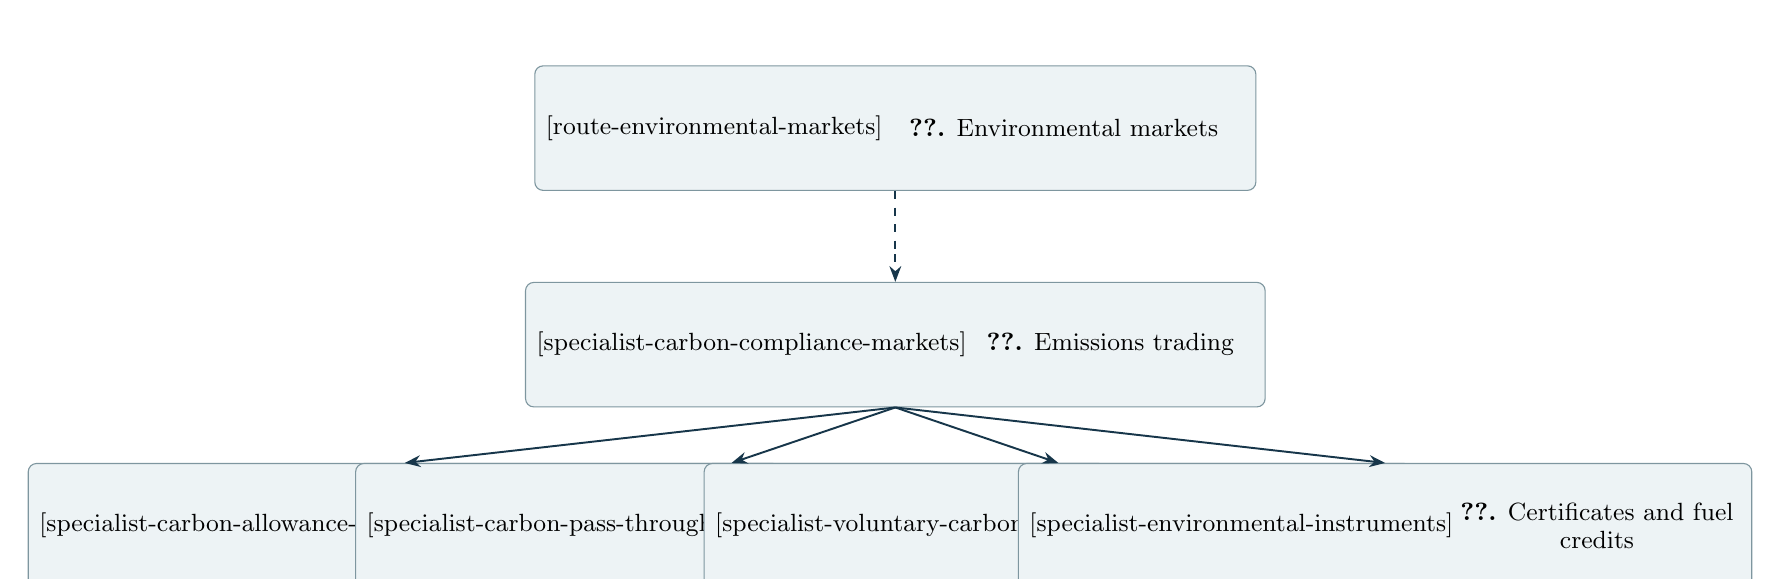
\begin{tikzpicture}[x=1cm,y=1cm]
\node[pathnode] (environmental-markets) at (6.23,0) {\MeasurePathNode{4.6cm}{\textbf{\ref*{route-environmental-markets}.} Environmental markets}\hyperref[route-environmental-markets]{\parbox[c][\pathnodeheight][c]{4.6cm}{\centering \textbf{\ref*{route-environmental-markets}.} Environmental markets}}};
\node[pathnode] (carbon-compliance-markets) at (6.23,-2.75) {\MeasurePathNode{3.65cm}{\textbf{\ref*{specialist-carbon-compliance-markets}.} Emissions trading}\hyperref[specialist-carbon-compliance-markets]{\parbox[c][\pathnodeheight][c]{3.65cm}{\centering \textbf{\ref*{specialist-carbon-compliance-markets}.} Emissions trading}}};
\node[pathnode] (carbon-allowance-derivatives) at (0.00,-5.05) {\MeasurePathNode{3.65cm}{\textbf{\ref*{specialist-carbon-allowance-derivatives}.} Allowance prices and derivatives}\hyperref[specialist-carbon-allowance-derivatives]{\parbox[c][\pathnodeheight][c]{3.65cm}{\centering \textbf{\ref*{specialist-carbon-allowance-derivatives}.} Allowance prices and derivatives}}};
\node[pathnode] (carbon-pass-through-leakage) at (4.15,-5.05) {\MeasurePathNode{3.65cm}{\textbf{\ref*{specialist-carbon-pass-through-leakage}.} Pass-through and leakage}\hyperref[specialist-carbon-pass-through-leakage]{\parbox[c][\pathnodeheight][c]{3.65cm}{\centering \textbf{\ref*{specialist-carbon-pass-through-leakage}.} Pass-through and leakage}}};
\node[pathnode] (voluntary-carbon-credits) at (8.30,-5.05) {\MeasurePathNode{3.65cm}{\textbf{\ref*{specialist-voluntary-carbon-credits}.} Voluntary credits}\hyperref[specialist-voluntary-carbon-credits]{\parbox[c][\pathnodeheight][c]{3.65cm}{\centering \textbf{\ref*{specialist-voluntary-carbon-credits}.} Voluntary credits}}};
\node[pathnode] (environmental-instruments) at (12.45,-5.05) {\MeasurePathNode{3.65cm}{\textbf{\ref*{specialist-environmental-instruments}.} Certificates and fuel credits}\hyperref[specialist-environmental-instruments]{\parbox[c][\pathnodeheight][c]{3.65cm}{\centering \textbf{\ref*{specialist-environmental-instruments}.} Certificates and fuel credits}}};
\draw[entryline] (environmental-markets.south) -- (6.23,-1.60);
\draw[entryline] (6.23,-1.60) -- (6.23,-1.60);
\draw[entryarrow] (6.23,-1.60) -- (carbon-compliance-markets.north);
\draw[patharrow] (carbon-compliance-markets.south) -- (carbon-allowance-derivatives.north);
\draw[patharrow] (carbon-compliance-markets.south) -- (carbon-pass-through-leakage.north);
\draw[patharrow] (carbon-compliance-markets.south) -- (voluntary-carbon-credits.north);
\draw[patharrow] (carbon-compliance-markets.south) -- (environmental-instruments.north);
\end{tikzpicture}\end{center}
\textbf{Overview checkpoint.} A section capstone: complete it after \hyperref[specialist-carbon-allowance-derivatives]{\ref*{specialist-carbon-allowance-derivatives}}, \hyperref[specialist-voluntary-carbon-credits]{\ref*{specialist-voluntary-carbon-credits}} and \hyperref[specialist-environmental-instruments]{\ref*{specialist-environmental-instruments}}.

\textbf{Bring these foundations with you.}\begin{itemize}
\item \hyperref[specialist-time-series-volatility]{Time-series econometrics and volatility forecasting} --- needed by \hyperref[specialist-carbon-allowance-derivatives]{Allowance prices and derivatives}.
\item \hyperref[specialist-power-ftr]{Power, storage and transmission rights} --- needed by \hyperref[specialist-carbon-pass-through-leakage]{Pass-through and leakage}.
\end{itemize}\hyperref[learning-map]{Return to the whole-guide DAG.}
\Needspace{12\baselineskip}
\subsection{Emissions trading: cap-and-trade design, banking and supply control}\label{specialist-carbon-compliance-markets}
\textbf{Specialist pathway.} In \hyperref[route-environmental-markets]{Environmental markets: emissions trading, carbon credits and certificates}.

\textbf{Outcome.} Explain how cap and trade reaches an emissions target at least cost, how allocation, auctions, banking, offsets, price collars and supply-adjustment rules shape the allowance price path, and how the EU ETS, its Market Stability Reserve and ETS2 implement them.

\textbf{Prerequisites.} Environmental markets overview; intertemporal optimisation.

\textbf{Review first.} \hyperref[route-environmental-markets]{Environmental markets: emissions trading, carbon credits and certificates}.

\textbf{Required readings, in order}
\begin{enumerate}\raggedright
\Needspace{5\baselineskip}\item \href{institutional_quantitative_finance_reading_list.pdf\#ec-montgomery-1972}{W. David Montgomery, ``Markets in Licenses and Efficient Pollution Control Programs''}\CataloguePage{389}\NoteKey{ec-montgomery-1972}\par \textbf{Foundations.} See why tradable permits reach an emissions target at least cost.
\Needspace{5\baselineskip}\item \href{institutional_quantitative_finance_reading_list.pdf\#carbon-rubin-banking-1996}{Jonathan D. Rubin, A Model of Intertemporal Emission Trading, Banking, and Borrowing}\CataloguePage{388}\NoteKey{carbon-rubin-banking-1996}\par \textbf{Valuation.} Value intertemporal compliance under allowance banking.
\Needspace{5\baselineskip}\item \href{institutional_quantitative_finance_reading_list.pdf\#ec-schmalensee-stavins-2017}{Richard Schmalensee and Robert N. Stavins, ``Lessons Learned from Three Decades of Experience with Cap and Trade''}\CataloguePage{389}\NoteKey{ec-schmalensee-stavins-2017}\par \textbf{Evidence.} Learn from three decades of cap-and-trade programmes.
\Needspace{5\baselineskip}\item \href{institutional_quantitative_finance_reading_list.pdf\#gp-cramton-kerr-2002}{Peter Cramton and Suzi Kerr, ``Tradeable carbon permit auctions''}\CataloguePage{390}\NoteKey{gp-cramton-kerr-2002}\par \textbf{Mechanics.} Design permit auctions instead of grandfathering.
\Needspace{5\baselineskip}\item \href{institutional_quantitative_finance_reading_list.pdf\#ec-ellerman-2016}{A. Denny Ellerman, Claudio Marcantonini and Aleksandar Zaklan, ``The European Union Emissions Trading System: Ten Years and Counting''}\CataloguePage{389}\NoteKey{ec-ellerman-2016}\par \textbf{Evidence.} Review the first ten years of the EU ETS.
\Needspace{5\baselineskip}\item \href{institutional_quantitative_finance_reading_list.pdf\#ec-perino-2018}{Grischa Perino, ``New EU ETS Phase 4 Rules Temporarily Puncture Waterbed''}\CataloguePage{389}\NoteKey{ec-perino-2018}\par \textbf{Mechanics.} See how the Market Stability Reserve ties the cap to market outcomes and temporarily punctures the waterbed.
\Needspace{5\baselineskip}\item \href{institutional_quantitative_finance_reading_list.pdf\#ec-borghesi-2023}{Simone Borghesi, Michael Pahle, Grischa Perino, Simon Quemin and Maximilian Willner, ``The Market Stability Reserve in the EU Emissions Trading System: A Critical Review''}\CataloguePage{389}\NoteKey{ec-borghesi-2023}\par \textbf{Evidence.} Assess the Market Stability Reserve against its objectives.
\Needspace{5\baselineskip}\item \href{institutional_quantitative_finance_reading_list.pdf\#carbon-eu-msr-2026}{European Commission, Directorate-General for Climate Action, Market Stability Reserve and 2025 Total Number of Allowances in Circulation; Dated 2026 TNAC communication}\CataloguePage{388}\NoteKey{carbon-eu-msr-2026}\par \textbf{Data.} Use the official count of allowances in circulation and the reserve intake.
\Needspace{5\baselineskip}\item \href{institutional_quantitative_finance_reading_list.pdf\#carbon-eu-market-report-2025}{European Commission, Directorate-General for Climate Action, 2025 Carbon Market Report: Report on the Functioning of the European Carbon Market in 2024; Commission report COM(2025) 735}\CataloguePage{388}\NoteKey{carbon-eu-market-report-2025}\par \textbf{Evidence.} Anchor EU ETS analysis to an official dated market report.
\Needspace{5\baselineskip}\item \href{institutional_quantitative_finance_reading_list.pdf\#ec-borenstein-2019}{Severin Borenstein, James Bushnell, Frank A. Wolak and Matthew Zaragoza-Watkins, ``Expecting the Unexpected: Emissions Uncertainty and Environmental Market Design''}\CataloguePage{389}\NoteKey{ec-borenstein-2019}\par \textbf{Evidence.} See emissions uncertainty push allowance prices to the floor or the ceiling.
\Needspace{5\baselineskip}\item \href{institutional_quantitative_finance_reading_list.pdf\#gp-eu-ets2-2026}{European Commission, Directorate-General for Climate Action, ETS2: buildings, road transport and additional sectors}\CataloguePage{390}\NoteKey{gp-eu-ets2-2026}\par \textbf{Mechanics.} Read ETS2 for buildings and road transport: upstream coverage, the 2028 start and its price-release trigger.
\end{enumerate}
\Needspace{5\baselineskip}\textbf{Checkpoint.} Build a two-period cap-and-trade model with banking and an abatement-cost curve, then add a Market Stability Reserve intake rule and a price floor. Using the official counts of allowances in circulation since 2017, show how reserve intake changed the effective cap, and compare ETS2's EUR 45 price-release trigger with the reserve rules of the existing EU ETS.

\textbf{Optional branches.} \href{institutional_quantitative_finance_reading_list.pdf\#carbon-richstein-msr-2015}{Simulate why the Market Stability Reserve might destabilise prices.}\BranchPage{388} \href{institutional_quantitative_finance_reading_list.pdf\#ec-fell-2012}{Compare soft and hard price collars.}\BranchPage{389}
\par{\small \hyperref[learning-map]{Learning pathway DAG} \textbar{} \hyperref[route-environmental-markets]{Section overview} \textbar{} \hyperref[map-environmental-markets]{Section DAG}\NoteKey{carbon-compliance-markets}}
\Needspace{12\baselineskip}
\subsection{Carbon allowance prices: drivers, derivatives, participants and hedging}\label{specialist-carbon-allowance-derivatives}
\textbf{Specialist pathway.} In \hyperref[route-environmental-markets]{Environmental markets: emissions trading, carbon credits and certificates}.

\textbf{Outcome.} Model EU allowance price dynamics and their fundamental drivers, price EUA futures and options with cost of carry, convenience yields and equilibrium models, read who trades and where prices are discovered, and hedge a compliance or CBAM exposure with December futures.

\textbf{Prerequisites.} Emissions trading: cap-and-trade design, banking and supply control; futures pricing and volatility models.

\textbf{Review first.} \hyperref[specialist-carbon-compliance-markets]{Emissions trading: cap-and-trade design, banking and supply control}; \hyperref[specialist-time-series-volatility]{Time-series econometrics and volatility forecasting}.

\textbf{Required readings, in order}
\begin{enumerate}\raggedright
\Needspace{5\baselineskip}\item \href{institutional_quantitative_finance_reading_list.pdf\#ec-hintermann-2010}{Beat Hintermann, ``Allowance Price Drivers in the First Phase of the EU ETS''}\CataloguePage{390}\NoteKey{ec-hintermann-2010}\par \textbf{Evidence.} Identify allowance price drivers in Phase I.
\Needspace{5\baselineskip}\item \href{institutional_quantitative_finance_reading_list.pdf\#gp-alberola-2008}{Emilie Alberola, Julien Chevallier and Benoît Chèze, ``Price drivers and structural breaks in European carbon prices 2005--2007''}\CataloguePage{391}\NoteKey{gp-alberola-2008}\par \textbf{Evidence.} Date the 2006 structural breaks and the fundamentals within each sub-period.
\Needspace{5\baselineskip}\item \href{institutional_quantitative_finance_reading_list.pdf\#ec-koch-2014}{Nicolas Koch, Sabine Fuss, Godefroy Grosjean and Ottmar Edenhofer, ``Causes of the EU ETS Price Drop: Recession, CDM, Renewable Policies or a Bit of Everything?---New Evidence''}\CataloguePage{390}\NoteKey{ec-koch-2014}\par \textbf{Evidence.} Test what explains the 2008--13 fall in EU allowance prices.
\Needspace{5\baselineskip}\item \href{institutional_quantitative_finance_reading_list.pdf\#gp-seifert-2008}{Jan Seifert, Marliese Uhrig-Homburg and Michael Wagner, ``Dynamic behavior of CO2 spot prices''}\CataloguePage{391}\NoteKey{gp-seifert-2008}\par \textbf{Theory.} Derive spot price dynamics from an equilibrium model of the scheme.
\Needspace{5\baselineskip}\item \href{institutional_quantitative_finance_reading_list.pdf\#gp-carmona-2010}{René Carmona, Max Fehr, Juri Hinz and Arnaud Porchet, ``Market Design for Emission Trading Schemes''}\CataloguePage{391}\NoteKey{gp-carmona-2010}\par \textbf{Theory.} Solve for equilibrium allowance and goods prices under cap and trade, and see windfall profits arise.
\Needspace{5\baselineskip}\item \href{institutional_quantitative_finance_reading_list.pdf\#gp-hitzemann-2018}{Steffen Hitzemann and Marliese Uhrig-Homburg, ``Equilibrium Price Dynamics of Emission Permits''}\CataloguePage{392}\NoteKey{gp-hitzemann-2018}\par \textbf{Valuation.} Price permits as contingent claims on aggregate emissions, with forward curves and options.
\Needspace{5\baselineskip}\item \href{institutional_quantitative_finance_reading_list.pdf\#gp-benz-truck-2009}{Eva Benz and Stefan Trück, ``Modeling the price dynamics of CO2 emission allowances''}\CataloguePage{391}\NoteKey{gp-benz-truck-2009}\par \textbf{Methods.} Model regime-switching volatility in allowance returns.
\Needspace{5\baselineskip}\item \href{institutional_quantitative_finance_reading_list.pdf\#ec-daskalakis-2009}{George Daskalakis, Dimitris Psychoyios and Raphael N. Markellos, ``Modeling CO2 Emission Allowance Prices and Derivatives: Evidence from the European Trading Scheme''}\CataloguePage{390}\NoteKey{ec-daskalakis-2009}\par \textbf{Valuation.} Price intra- and inter-phase futures and options when banking between phases is prohibited.
\Needspace{5\baselineskip}\item \href{institutional_quantitative_finance_reading_list.pdf\#gp-truck-weron-2016}{Stefan Trück and Rafał Weron, ``Convenience Yields and Risk Premiums in the EU‐ETS---Evidence from the Kyoto Commitment Period''}\CataloguePage{391}\NoteKey{gp-truck-weron-2016}\par \textbf{Evidence.} Measure negative convenience yields and risk premia in EUA futures.
\Needspace{5\baselineskip}\item \href{institutional_quantitative_finance_reading_list.pdf\#gp-rittler-2012}{Daniel Rittler, ``Price discovery and volatility spillovers in the European Union emissions trading scheme: A high-frequency analysis''}\CataloguePage{392}\NoteKey{gp-rittler-2012}\par \textbf{Evidence.} See the futures market lead price discovery and volatility.
\Needspace{5\baselineskip}\item \href{institutional_quantitative_finance_reading_list.pdf\#gp-cludius-betz-2020}{Johanna Cludius and Regina Betz, ``The Role of Banks in EU Emissions Trading''}\CataloguePage{392}\NoteKey{gp-cludius-betz-2020}\par \textbf{Evidence.} Learn how banks and brokers intermediate allowance trading.
\Needspace{5\baselineskip}\item \href{institutional_quantitative_finance_reading_list.pdf\#gp-esma-2022}{European Securities and Markets Authority, Final Report: Emission allowances and associated derivatives (ESMA70-445-38)}\CataloguePage{392}\NoteKey{gp-esma-2022}\par \textbf{Evidence.} Read the supervisor's map of who holds EUA derivatives and its recommendations.
\Needspace{5\baselineskip}\item \href{institutional_quantitative_finance_reading_list.pdf\#gp-quemin-pahle-2023}{Simon Quemin and Michael Pahle, ``Financials threaten to undermine the functioning of emissions markets''}\CataloguePage{392}\NoteKey{gp-quemin-pahle-2023}\par \textbf{Regulation.} Weigh the functions and risks of financial participants and how to monitor speculation.
\Needspace{5\baselineskip}\item \href{institutional_quantitative_finance_reading_list.pdf\#carbon-ice-eua-futures}{ICE Endex, EUA Futures Contract Specification}\CataloguePage{391}\NoteKey{carbon-ice-eua-futures}\par \textbf{Implementation.} Map the exchange contract and delivery lifecycle of an allowance hedge.
\end{enumerate}
\Needspace{5\baselineskip}\textbf{Checkpoint.} Assemble daily December EUA futures settlements and spot prices since 2008 with the annual allowances in circulation, auction volumes and the dates of major reform decisions. Fit a regime-switching volatility model, estimate the futures convenience yield each year, and explain the price path in Phase II, after the reserve reform and in 2022--26 with fuel-switching prices and policy events. Then hedge a manufacturer's 2027 compliance obligation and a 2027 CBAM import exposure with December futures, and state how certificate pricing (quarterly averages in 2026, weekly from 2027) creates basis against the hedge.

\textbf{Optional branches.} \href{institutional_quantitative_finance_reading_list.pdf\#gp-paolella-taschini-2008}{Forecast value at risk for EU CO2 and US SO2 allowances.}\BranchPage{391} \href{institutional_quantitative_finance_reading_list.pdf\#gp-chesney-taschini-2012}{Derive endogenous permit dynamics and a closed-form option price.}\BranchPage{392} \href{institutional_quantitative_finance_reading_list.pdf\#w3-fuchs-carbon-vix}{Measure carbon-price uncertainty and decarbonisation investment.}\BranchPage{391}
\par{\small \hyperref[learning-map]{Learning pathway DAG} \textbar{} \hyperref[route-environmental-markets]{Section overview} \textbar{} \hyperref[map-environmental-markets]{Section DAG}\NoteKey{carbon-allowance-derivatives}}
\Needspace{12\baselineskip}
\subsection{Carbon costs in power and industry: pass-through, leakage and border adjustment}\label{specialist-carbon-pass-through-leakage}
\textbf{Specialist pathway.} In \hyperref[route-environmental-markets]{Environmental markets: emissions trading, carbon credits and certificates}.

\textbf{Outcome.} Measure how allowance costs pass into electricity and product prices, test for emissions leakage and effects on regulated firms, and evaluate free allocation and border carbon adjustment, including the EU CBAM, as responses.

\textbf{Prerequisites.} Emissions trading: cap-and-trade design, banking and supply control; Power, storage and transmission rights (25.3) for the merit order and marginal plants; panel econometrics.

\textbf{Review first.} \hyperref[specialist-carbon-compliance-markets]{Emissions trading: cap-and-trade design, banking and supply control}; \hyperref[specialist-power-ftr]{Power, storage and transmission rights}.

\textbf{Required readings, in order}
\begin{enumerate}\raggedright
\Needspace{5\baselineskip}\item \href{institutional_quantitative_finance_reading_list.pdf\#gp-sijm-2006}{Jos Sijm, Karsten Neuhoff and Yihsu Chen, ``CO2 cost pass-through and windfall profits in the power sector''}\CataloguePage{393}\NoteKey{gp-sijm-2006}\par \textbf{Evidence.} Estimate CO2 cost pass-through and windfall profits in EU power.
\Needspace{5\baselineskip}\item \href{institutional_quantitative_finance_reading_list.pdf\#gp-fabra-reguant-2014}{Natalia Fabra and Mar Reguant, ``Pass-Through of Emissions Costs in Electricity Markets''}\CataloguePage{393}\NoteKey{gp-fabra-reguant-2014}\par \textbf{Evidence.} See emissions costs passed almost fully into electricity prices, and why.
\Needspace{5\baselineskip}\item \href{institutional_quantitative_finance_reading_list.pdf\#gp-hintermann-2016}{Beat Hintermann, ``Pass-Through of CO2 Emission Costs to Hourly Electricity Prices in Germany''}\CataloguePage{393}\NoteKey{gp-hintermann-2016}\par \textbf{Evidence.} Identify hourly pass-through from the marginal plant.
\Needspace{5\baselineskip}\item \href{institutional_quantitative_finance_reading_list.pdf\#gp-fowlie-2009}{Meredith L Fowlie, ``Incomplete Environmental Regulation, Imperfect Competition, and Emissions Leakage''}\CataloguePage{394}\NoteKey{gp-fowlie-2009}\par \textbf{Theory.} Model leakage under incomplete regulation and imperfect competition.
\Needspace{5\baselineskip}\item \href{institutional_quantitative_finance_reading_list.pdf\#gp-fowlie-reguant-ryan-2016}{Meredith Fowlie, Mar Reguant and Stephen P. Ryan, ``Market-Based Emissions Regulation and Industry Dynamics''}\CataloguePage{394}\NoteKey{gp-fowlie-reguant-ryan-2016}\par \textbf{Evidence.} Weigh market power against leakage in cement under carbon pricing.
\Needspace{5\baselineskip}\item \href{institutional_quantitative_finance_reading_list.pdf\#gp-martin-2014}{Ralf Martin, Mirabelle Muûls, Laure B. de Preux and Ulrich J. Wagner, ``Industry Compensation under Relocation Risk: A Firm-Level Analysis of the EU Emissions Trading Scheme''}\CataloguePage{394}\NoteKey{gp-martin-2014}\par \textbf{Evidence.} Test whether free allocation matches relocation risk.
\Needspace{5\baselineskip}\item \href{institutional_quantitative_finance_reading_list.pdf\#gp-naegele-zaklan-2019}{Helene Naegele and Aleksandar Zaklan, ``Does the EU ETS cause carbon leakage in European manufacturing?''}\CataloguePage{394}\NoteKey{gp-naegele-zaklan-2019}\par \textbf{Evidence.} Look for leakage in carbon embodied in European trade.
\Needspace{5\baselineskip}\item \href{institutional_quantitative_finance_reading_list.pdf\#gp-dechezlepretre-2022}{Antoine Dechezleprêtre, Caterina Gennaioli, Ralf Martin, Mirabelle Muûls and Thomas Stoerk, ``Searching for carbon leaks in multinational companies''}\CataloguePage{394}\NoteKey{gp-dechezlepretre-2022}\par \textbf{Evidence.} Look for leakage inside multinational firms.
\Needspace{5\baselineskip}\item \href{institutional_quantitative_finance_reading_list.pdf\#gp-colmer-2025}{Jonathan Colmer, Ralf Martin, Mirabelle Muûls and Ulrich J Wagner, ``Does Pricing Carbon Mitigate Climate Change? Firm-Level Evidence from the European Union Emissions Trading System''}\CataloguePage{394}\NoteKey{gp-colmer-2025}\par \textbf{Evidence.} Measure firm-level emission cuts under the EU ETS without output losses.
\Needspace{5\baselineskip}\item \href{institutional_quantitative_finance_reading_list.pdf\#gp-bohringer-2022}{Christoph Böhringer, Carolyn Fischer, Knut Einar Rosendahl and Thomas Fox Rutherford, ``Potential impacts and challenges of border carbon adjustments''}\CataloguePage{394}\NoteKey{gp-bohringer-2022}\par \textbf{Foundations.} Assess what border carbon adjustments can achieve under legal and practical limits.
\Needspace{5\baselineskip}\item \href{institutional_quantitative_finance_reading_list.pdf\#gp-clausing-wolfram-2023}{Kimberly A. Clausing and Catherine Wolfram, ``Carbon Border Adjustments, Climate Clubs, and Subsidy Races When Climate Policies Vary''}\CataloguePage{395}\NoteKey{gp-clausing-wolfram-2023}\par \textbf{Foundations.} Distinguish free-riding from competitiveness spillovers and the role of climate clubs.
\Needspace{5\baselineskip}\item \href{institutional_quantitative_finance_reading_list.pdf\#ec-cbam-2026}{European Commission, Directorate-General for Taxation and Customs Union, Carbon Border Adjustment Mechanism (CBAM): definitive regime and price of CBAM certificates}\CataloguePage{393}\NoteKey{ec-cbam-2026}\par \textbf{Mechanics.} Read the CBAM definitive regime from 2026: declarants buy certificates priced from EU ETS auctions.
\end{enumerate}
\Needspace{5\baselineskip}\textbf{Checkpoint.} For one bidding zone, regress hourly day-ahead prices on the allowance cost of the marginal plant to estimate pass-through by load level. For one CBAM sector, compare the free-allocation benefit with the CBAM certificate cost for an importer in 2026, and test whether the sector's net imports respond to the EUA price.

\textbf{Optional branches.} \href{institutional_quantitative_finance_reading_list.pdf\#gp-branger-2016}{Test for short-run leakage in EU cement and steel.}\BranchPage{395} \href{institutional_quantitative_finance_reading_list.pdf\#gp-fowlie-reguant-2022}{Calibrate output-based subsidies to industry leakage risk.}\BranchPage{395} \href{institutional_quantitative_finance_reading_list.pdf\#ec-martin-muuls-wagner-2016}{Review the evidence on regulated firms after ten years.}\BranchPage{393} \href{institutional_quantitative_finance_reading_list.pdf\#ec-bayer-aklin-2020}{Estimate the emissions reductions of the EU ETS despite low prices.}\BranchPage{393} \href{institutional_quantitative_finance_reading_list.pdf\#ec-kanzig-2023}{Trace the economic effects of EU carbon-policy surprises.}\BranchPage{393}
\par{\small \hyperref[learning-map]{Learning pathway DAG} \textbar{} \hyperref[route-environmental-markets]{Section overview} \textbar{} \hyperref[map-environmental-markets]{Section DAG}\NoteKey{carbon-pass-through-leakage}}
\Needspace{12\baselineskip}
\subsection{Voluntary carbon and biodiversity credits: integrity, pricing and Article 6}\label{specialist-voluntary-carbon-credits}
\textbf{Specialist pathway.} In \hyperref[route-environmental-markets]{Environmental markets: emissions trading, carbon credits and certificates}.

\textbf{Outcome.} Judge whether a voluntary credit represents a real, additional and durable reduction, explain how baselines, ratings and buyer demand shape credit prices, distinguish voluntary claims from Article 6 transfers, and apply the same tests to biodiversity credits.

\textbf{Prerequisites.} Emissions trading: cap-and-trade design, banking and supply control; causal inference for baselines and additionality.

\textbf{Review first.} \hyperref[specialist-carbon-compliance-markets]{Emissions trading: cap-and-trade design, banking and supply control}.

\textbf{Required readings, in order}
\begin{enumerate}\raggedright
\Needspace{5\baselineskip}\item \href{institutional_quantitative_finance_reading_list.pdf\#carbon-icvcm-ccp-2024}{Integrity Council for the Voluntary Carbon Market, Core Carbon Principles and Assessment Framework, Version 2; Current CCP program and methodology assessments}\CataloguePage{395}\NoteKey{carbon-icvcm-ccp-2024}\par \textbf{Mechanics.} Separate voluntary carbon-credit integrity screens from compliance units.
\Needspace{5\baselineskip}\item \href{institutional_quantitative_finance_reading_list.pdf\#gp-bento-kanbur-leard-2016}{Antonio Bento, Ravi Kanbur and Benjamin Leard, ``On the importance of baseline setting in carbon offsets markets''}\CataloguePage{396}\NoteKey{gp-bento-kanbur-leard-2016}\par \textbf{Theory.} See how baseline stringency balances over- and under-crediting.
\Needspace{5\baselineskip}\item \href{institutional_quantitative_finance_reading_list.pdf\#gp-agrawal-2026}{Vishal V. Agrawal, Soudipta Chakraborty and Şafak Yücel, ``Additionality of Carbon Offsets: Project-Specific vs. Standardized Baselines''}\CataloguePage{397}\NoteKey{gp-agrawal-2026}\par \textbf{Theory.} Compare project-specific and standardised baselines when project revenue is private.
\Needspace{5\baselineskip}\item \href{institutional_quantitative_finance_reading_list.pdf\#ec-calel-2025}{Raphael Calel, Jonathan Colmer, Antoine Dechezleprêtre and Matthieu Glachant, ``Do Carbon Offsets Offset Carbon?''}\CataloguePage{395}\NoteKey{ec-calel-2025}\par \textbf{Evidence.} Estimate how many offset credits went to projects that would have been built anyway.
\Needspace{5\baselineskip}\item \href{institutional_quantitative_finance_reading_list.pdf\#ec-west-2023}{Thales A. P. West, Sven Wunder, Erin O. Sills, Jan Börner, Sami W. Rifai, Alexandra N. Neidermeier, Gabriel P. Frey and Andreas Kontoleon, ``Action Needed to Make Carbon Offsets from Forest Conservation Work for Climate Change Mitigation''}\CataloguePage{395}\NoteKey{ec-west-2023}\par \textbf{Evidence.} See forest-conservation credits rest on baselines that overstate avoided deforestation.
\Needspace{5\baselineskip}\item \href{institutional_quantitative_finance_reading_list.pdf\#ec-badgley-2022}{Grayson Badgley, Jeremy Freeman, Joseph J. Hamman, Barbara Haya, Anna T. Trugman, William R. L. Anderegg and Danny Cullenward, ``Systematic Over-crediting in California's Forest Carbon Offsets Program''}\CataloguePage{396}\NoteKey{ec-badgley-2022}\par \textbf{Evidence.} Measure over-crediting in California's forest offsets.
\Needspace{5\baselineskip}\item \href{institutional_quantitative_finance_reading_list.pdf\#gp-haya-2023}{Barbara K. Haya, Samuel Evans, Letty Brown, Jacob Bukoski, Van Butsic, Bodie Cabiyo, Rory Jacobson, Amber Kerr, Matthew Potts and Daniel L. Sanchez, ``Comprehensive review of carbon quantification by improved forest management offset protocols''}\CataloguePage{397}\NoteKey{gp-haya-2023}\par \textbf{Evidence.} Check improved-forest-management protocols against the science.
\Needspace{5\baselineskip}\item \href{institutional_quantitative_finance_reading_list.pdf\#gp-gill-wiehl-2024}{Annelise Gill-Wiehl, Daniel M. Kammen and Barbara K. Haya, ``Pervasive over-crediting from cookstove offset methodologies''}\CataloguePage{397}\NoteKey{gp-gill-wiehl-2024}\par \textbf{Evidence.} Quantify over-crediting in cookstove methodologies.
\Needspace{5\baselineskip}\item \href{institutional_quantitative_finance_reading_list.pdf\#ec-probst-2024}{Benedict S. Probst, Malte Toetzke, Andreas Kontoleon, Laura Díaz Anadón, Jan C. Minx, Barbara K. Haya, Lambert Schneider, Philipp A. Trotter, Thales A. P. West, Annelise Gill-Wiehl and Volker H. Hoffmann, ``Systematic Assessment of the Achieved Emission Reductions of Carbon Crediting Projects''}\CataloguePage{396}\NoteKey{ec-probst-2024}\par \textbf{Evidence.} Compare credits issued with emission reductions achieved across project types.
\Needspace{5\baselineskip}\item \href{institutional_quantitative_finance_reading_list.pdf\#gp-trencher-2024}{Gregory Trencher, Sascha Nick, Jordan Carlson and Matthew Johnson, ``Demand for low-quality offsets by major companies undermines climate integrity of the voluntary carbon market''}\CataloguePage{397}\NoteKey{gp-trencher-2024}\par \textbf{Evidence.} See which credits the largest corporate buyers retire.
\Needspace{5\baselineskip}\item \href{institutional_quantitative_finance_reading_list.pdf\#gp-berg-2025}{Florian Berg, Marco Ceccarelli, Florian Heeb, Alexey Ivashchenko, Roberto Rigobon and Remco C. J. Zwinkels, ``The Market for Voluntary Carbon Offsets''}\CataloguePage{397}\NoteKey{gp-berg-2025}\par \textbf{Evidence.} Explain dispersed voluntary-credit prices by project, buyer and trade characteristics.
\Needspace{5\baselineskip}\item \href{institutional_quantitative_finance_reading_list.pdf\#gp-schneider-2019}{Lambert Schneider, Maosheng Duan, Robert Stavins, Kelley Kizzier, Derik Broekhoff, Frank Jotzo, Harald Winkler, Michael Lazarus, Andrew Howard and Christina Hood, ``Double counting and the Paris Agreement rulebook''}\CataloguePage{396}\NoteKey{gp-schneider-2019}\par \textbf{Mechanics.} Understand double counting and corresponding adjustments under Article 6.
\Needspace{5\baselineskip}\item \href{institutional_quantitative_finance_reading_list.pdf\#gp-eu-2040-2026}{European Commission, Directorate-General for Climate Action, 2040 climate target}\CataloguePage{398}\NoteKey{gp-eu-2040-2026}\par \textbf{Regulation.} See the EU allow up to 5 per cent international credits toward its 2040 target.
\Needspace{5\baselineskip}\item \href{institutional_quantitative_finance_reading_list.pdf\#gp-cftc-vcc-2024}{Commodity Futures Trading Commission, Commission Guidance Regarding the Listing of Voluntary Carbon Credit Derivative Contracts; withdrawal notice}\CataloguePage{397}\NoteKey{gp-cftc-vcc-2024}\par \textbf{Implementation.} Specify the quality and delivery terms of a credit derivative, noting the guidance was withdrawn.
\Needspace{5\baselineskip}\item \href{institutional_quantitative_finance_reading_list.pdf\#add-biodiversity-framework}{International Advisory Panel on Biodiversity Credits, Framework for High Integrity Biodiversity Credit Markets}\CataloguePage{399}\NoteKey{add-biodiversity-framework}\par \textbf{Mechanics.} Read the biodiversity-credit framework and its nonfungibility constraint.
\Needspace{5\baselineskip}\item \href{institutional_quantitative_finance_reading_list.pdf\#add-biodiversity-principles}{Biodiversity Credit Alliance, IAPB and World Economic Forum, High-level Principles to Guide the Biodiversity Credit Market; May 2025 white paper}\CataloguePage{399}\NoteKey{add-biodiversity-principles}\par \textbf{Implementation.} Test claim language and project governance before treating a credit as financeable.
\end{enumerate}
\Needspace{5\baselineskip}\textbf{Checkpoint.} Make a lifecycle ledger for one voluntary credit: methodology, baseline, crediting period, buffer contribution, any ICVCM label, and whether it carries a corresponding adjustment for Article 6 use. State what the over-crediting evidence for its project type implies for its additionality, compare its price with other project types using the dealer-price evidence, and list the quality and delivery terms a futures contract on it would need. Separately map a biodiversity credit's measurement, governance and claim rules; mark unsupported fungibility or banking fields inapplicable.

\textbf{Optional branches.} \href{institutional_quantitative_finance_reading_list.pdf\#w3-rodemeier-carbon-offsets}{Measure willingness to pay for offsets.}\BranchPage{396} \href{institutional_quantitative_finance_reading_list.pdf\#carbon-balmford-permanence-2023}{Value impermanent carbon credits.}\BranchPage{396} \href{institutional_quantitative_finance_reading_list.pdf\#carbon-swinfield-overcrediting-2026}{Learn from over-crediting to ensure additionality in forest credits.}\BranchPage{396} \href{institutional_quantitative_finance_reading_list.pdf\#w3-flammer-biodiversity}{Study biodiversity finance structures.}\BranchPage{399}
\par{\small \hyperref[learning-map]{Learning pathway DAG} \textbar{} \hyperref[route-environmental-markets]{Section overview} \textbar{} \hyperref[map-environmental-markets]{Section DAG}\NoteKey{voluntary-carbon-credits}}
\Needspace{12\baselineskip}
\subsection{Renewable energy certificates and low-carbon fuel credits: RECs, RINs and LCFS}\label{specialist-environmental-instruments}
\textbf{Specialist pathway.} In \hyperref[route-environmental-markets]{Environmental markets: emissions trading, carbon credits and certificates}.

\textbf{Outcome.} Distinguish REC, RIN and LCFS credits by eligibility, vintage, banking and retirement, price them from their compliance fundamentals, and judge what renewable portfolio standards and fuel standards achieve.

\textbf{Prerequisites.} Emissions trading: cap-and-trade design, banking and supply control; regulatory asset design and lifecycle data.

\textbf{Review first.} \hyperref[specialist-carbon-compliance-markets]{Emissions trading: cap-and-trade design, banking and supply control}.

\textbf{Required readings, in order}
\begin{enumerate}\raggedright
\Needspace{5\baselineskip}\item \href{institutional_quantitative_finance_reading_list.pdf\#gp-schmalensee-2012}{Richard Schmalensee, ``Evaluating Policies to Increase Electricity Generation from Renewable Energy''}\CataloguePage{400}\NoteKey{gp-schmalensee-2012}\par \textbf{Foundations.} Compare renewable portfolio standards with feed-in tariffs and see how REC markets fall short.
\Needspace{5\baselineskip}\item \href{institutional_quantitative_finance_reading_list.pdf\#add-rec-standard}{Center for Resource Solutions / Green-e, Renewable Energy Standard for Canada and the United States; certification criteria}\CataloguePage{398}\NoteKey{add-rec-standard}\par \textbf{Mechanics.} Read renewable-certificate eligibility, vintage and claims rules.
\Needspace{5\baselineskip}\item \href{institutional_quantitative_finance_reading_list.pdf\#add-rec-data}{Center for Resource Solutions / Green-e, Annual Verification Reports}\CataloguePage{398}\NoteKey{add-rec-data}\par \textbf{Data.} Measure certified transaction volumes and geography; obtain separate registry records for certificate-level issuance and retirement.
\Needspace{5\baselineskip}\item \href{institutional_quantitative_finance_reading_list.pdf\#gapclose-nepool-rec-reports}{NEPOOL Generation Information System, Public Reports}\CataloguePage{398}\NoteKey{gapclose-nepool-rec-reports}\par \textbf{Data.} Distinguish registry issuance, transfer and residual-mix counts from certificate-level retirement and programme certification.
\Needspace{5\baselineskip}\item \href{institutional_quantitative_finance_reading_list.pdf\#w5-hulshof-recs}{Daan Hulshof, Catrinus Jepma and Machiel Mulder, ``Performance of markets for European renewable energy certificates''}\CataloguePage{399}\NoteKey{w5-hulshof-recs}\par \textbf{Evidence.} Assess liquidity and price formation in European guarantee-of-origin markets.
\Needspace{5\baselineskip}\item \href{institutional_quantitative_finance_reading_list.pdf\#gp-coulon-2015}{Michael Coulon, Javad Khazaei and Warren B. Powell, ``SMART-SREC: A stochastic model of the New Jersey solar renewable energy certificate market''}\CataloguePage{400}\NoteKey{gp-coulon-2015}\par \textbf{Valuation.} Model solar certificate prices with a supply response and market rules.
\Needspace{5\baselineskip}\item \href{institutional_quantitative_finance_reading_list.pdf\#add-rin-mechanics}{U.S. Environmental Protection Agency, Renewable Identification Numbers (RINs) under the Renewable Fuel Standard Program}\CataloguePage{398}\NoteKey{add-rin-mechanics}\par \textbf{Mechanics.} Define RIN generation, separation and compliance obligations.
\Needspace{5\baselineskip}\item \href{institutional_quantitative_finance_reading_list.pdf\#gp-gerveni-2026}{Maria Gerveni, Todd Hubbs, Scott H. Irwin and James H. Stock, ``The Biofuels Blueprint: Understanding the U.S. Renewable Fuel Standard''}\CataloguePage{401}\NoteKey{gp-gerveni-2026}\par \textbf{Foundations.} Review two decades of the Renewable Fuel Standard, RIN prices and compliance costs.
\Needspace{5\baselineskip}\item \href{institutional_quantitative_finance_reading_list.pdf\#gp-irwin-2020}{Scott H. Irwin, Kristen McCormack and James H. Stock, ``The Price of Biodiesel RINs and Economic Fundamentals''}\CataloguePage{400}\NoteKey{gp-irwin-2020}\par \textbf{Valuation.} Price the D4 RIN from the biodiesel--diesel spread and the tax credit.
\Needspace{5\baselineskip}\item \href{institutional_quantitative_finance_reading_list.pdf\#w5-knittel-rin-passthrough}{Christopher R. Knittel, Ben S. Meiselman and James H. Stock, ``The Pass-Through of RIN Prices to Wholesale and Retail Fuels under the Renewable Fuel Standard''}\CataloguePage{399}\NoteKey{w5-knittel-rin-passthrough}\par \textbf{Evidence.} Trace RIN pass-through to wholesale and retail fuel prices.
\Needspace{5\baselineskip}\item \href{institutional_quantitative_finance_reading_list.pdf\#add-rin-data}{U.S. Environmental Protection Agency, RIN Trades and Price Information; public RFS data}\CataloguePage{398}\NoteKey{add-rin-data}\par \textbf{Data.} Use EPA transaction and retirement series with their reporting lag.
\Needspace{5\baselineskip}\item \href{institutional_quantitative_finance_reading_list.pdf\#add-rin-rule2026}{U.S. Environmental Protection Agency, Final Renewable Fuel Standards for 2026 and 2027}\CataloguePage{399}\NoteKey{add-rin-rule2026}\par \textbf{Regulation.} Check the 2026--27 renewable-fuel rule and its effective status.
\Needspace{5\baselineskip}\item \href{institutional_quantitative_finance_reading_list.pdf\#gp-holland-2009}{Stephen P Holland, Jonathan E Hughes and Christopher R Knittel, ``Greenhouse Gas Reductions under Low Carbon Fuel Standards?''}\CataloguePage{400}\NoteKey{gp-holland-2009}\par \textbf{Theory.} See why a low carbon fuel standard can raise emissions and cannot be efficient.
\Needspace{5\baselineskip}\item \href{institutional_quantitative_finance_reading_list.pdf\#gp-yeh-2016}{Sonia Yeh, Julie Witcover, Gabriel E. Lade and Daniel Sperling, ``A review of low carbon fuel policies: Principles, program status and future directions''}\CataloguePage{400}\NoteKey{gp-yeh-2016}\par \textbf{Mechanics.} Compare LCFS design and programmes in California, the EU, British Columbia and Oregon.
\Needspace{5\baselineskip}\item \href{institutional_quantitative_finance_reading_list.pdf\#gp-carb-lcfs-2026}{California Air Resources Board, Monthly LCFS Credit Transfer Activity Reports; LCFS regulation page}\CataloguePage{401}\NoteKey{gp-carb-lcfs-2026}\par \textbf{Data.} Use CARB's monthly LCFS credit-transfer volumes and prices.
\end{enumerate}
\Needspace{5\baselineskip}\textbf{Checkpoint.} Make lifecycle ledgers for a REC, a D4 or D6 RIN and an LCFS credit: generation or issuance, separation, transfer, banking limits and retirement. Reconcile NEPOOL issuance, transfer and residual-mix definitions with the chosen reporting periods and compare their scope with Green-e programme totals; do not populate a specific REC retirement without serial-level evidence, or mix CPEC with REC counts. Rebuild a D4 RIN fundamental price from the biodiesel--diesel spread and the tax-credit status and compare it with EPA weekly prices, then chart CARB's monthly LCFS credit prices since 2023 and mark the effective date of the amended regulation.

\textbf{Optional branches.} \href{institutional_quantitative_finance_reading_list.pdf\#w5-lade-rfs-shocks}{See policy news move RIN prices.}\BranchPage{399} \href{institutional_quantitative_finance_reading_list.pdf\#gp-lade-linlawell-2021}{Compare renewable fuel mandates with and without cost containment.}\BranchPage{400} \href{institutional_quantitative_finance_reading_list.pdf\#w5-bento-garg-kaffine}{See general-equilibrium effects of a renewable portfolio standard.}\BranchPage{400} \href{institutional_quantitative_finance_reading_list.pdf\#gp-upton-snyder-2017}{Compare prices, generation and emissions in states with and without portfolio standards.}\BranchPage{401}
\par{\small \hyperref[learning-map]{Learning pathway DAG} \textbar{} \hyperref[route-environmental-markets]{Section overview} \textbar{} \hyperref[map-environmental-markets]{Section DAG}\NoteKey{environmental-instruments}}
\clearpage
\part{Private capital, real assets and insurance}\label{part-private-real-insurance}
Evaluate long-dated contractual cash flows, asset rights and contingent claims.

\textbf{Sections in learning order}\begin{enumerate}
\item[\ref*{route-private-capital-allocator}.] \hyperref[route-private-capital-allocator]{Private-capital allocator} --- Study ownership and credit claims, expand to other contractual cash flows, then evaluate fund liquidity.
\item[\ref*{route-real-asset-investor}.] \hyperref[route-real-asset-investor]{Real-asset investor} --- Begin with property and infrastructure valuation, then examine leased equipment, resource rights and collectibles.
\item[\ref*{route-insurance-climate-risk}.] \hyperref[route-insurance-climate-risk]{Insurance and climate-linked risk} --- Build from insured loss and longevity claims toward weather payoffs and sidecar capital structures.
\end{enumerate}
\hyperref[learning-map]{Return to the learning pathway DAG.}
\clearpage
\section{Private-capital allocator}\label{route-private-capital-allocator}
\label{route-12}
\textbf{Learning sequence.} Study ownership and credit claims, expand to other contractual cash flows, then evaluate fund liquidity.

\textbf{Section goals.} Across its pathways, this section teaches you to:
\begin{itemize}[leftmargin=1.4em,itemsep=0pt,topsep=1pt]
\item measure private-fund performance with PME, direct alpha and cash-flow returns (\hyperref[specialist-pe-performance-measurement]{\ref*{specialist-pe-performance-measurement}})
\item connect private-equity and venture security terms to fund performance (\hyperref[specialist-private-equity-vc]{\ref*{specialist-private-equity-vc}})
\item underwrite direct loans by covenant, collateral and restructuring waterfall (\hyperref[specialist-private-credit-workouts]{\ref*{specialist-private-credit-workouts}})
\item model trade-finance and purchased-receivables risk (\hyperref[specialist-trade-receivables]{\ref*{specialist-trade-receivables}})
\item value music and pharmaceutical royalty interests (\hyperref[specialist-royalty-rights]{\ref*{specialist-royalty-rights}})
\item underwrite litigation-finance cash flows (\hyperref[specialist-litigation-finance-claims]{\ref*{specialist-litigation-finance-claims}})
\item model capital calls, NAV leverage and redemptions in fund vehicles (\hyperref[specialist-fund-liquidity]{\ref*{specialist-fund-liquidity}})
\end{itemize}
\textbf{Overview outcome.} Measure a fund's performance from dated investor cash flows against a public benchmark, and show when delayed exits, extra calls, NAV financing or lower appraisals force an allocator to sell liquid assets or cut new commitments.

\textbf{Prerequisites.} Common toolkit; discounting, fund cash flows, debt seniority and public-market benchmarks.

\textbf{Review first.} \hyperref[route-common-toolkit]{Common toolkit}.

\textbf{Required readings, in order}
\begin{enumerate}\raggedright
\Needspace{5\baselineskip}\item \href{institutional_quantitative_finance_reading_list.pdf\#pe-kaplan-schoar-2005}{Steven N. Kaplan and Antoinette Schoar, Private Equity Performance: Returns, Persistence, and Capital Flows}\CataloguePage{402}\NoteKey{pe-kaplan-schoar-2005}\par Introduce fund cash-flow performance, persistence and the need for a suitable vintage comparison.
\Needspace{5\baselineskip}\item \href{institutional_quantitative_finance_reading_list.pdf\#pe-metrick-yasuda-2010}{Andrew Metrick and Ayako Yasuda, The Economics of Private Equity Funds}\CataloguePage{402}\NoteKey{pe-metrick-yasuda-2010}\par Decompose the economics of management fees, carry and fund-level incentives.
\Needspace{5\baselineskip}\item \href{institutional_quantitative_finance_reading_list.pdf\#pe-harris-jenkinson-kaplan-2014}{Robert S. Harris, Tim Jenkinson, and Steven N. Kaplan, Private Equity Performance: What Do We Know?}\CataloguePage{402}\NoteKey{pe-harris-jenkinson-kaplan-2014}\par Compare private-equity results with public-market alternatives using investor cash flows.
\Needspace{5\baselineskip}\item \href{institutional_quantitative_finance_reading_list.pdf\#pc-erel-flanagan-weisbach-2024}{Isil Erel, Thomas Flanagan, and Michael S. Weisbach, Risk-Adjusting the Returns to Private Debt Funds}\CataloguePage{411}\NoteKey{pc-erel-flanagan-weisbach-2024}\par Risk-adjust private-debt fund returns instead of treating contractual yield as net alpha.
\Needspace{5\baselineskip}\item \href{institutional_quantitative_finance_reading_list.pdf\#re-geltner-unsmoothing-1993}{David M. Geltner, Estimating Market Values from Appraised Values without Assuming an Efficient Market}\CataloguePage{419}\NoteKey{re-geltner-unsmoothing-1993}\par Recognise how appraisal smoothing distorts measured volatility and cross-asset comparisons.
\Needspace{5\baselineskip}\item \href{institutional_quantitative_finance_reading_list.pdf\#depth-pe-robinson-sensoy-cashflows}{David T. Robinson and Berk A. Sensoy, Cyclicality, Performance Measurement, and Cash Flow Liquidity in Private Equity}\CataloguePage{409}\NoteKey{depth-pe-robinson-sensoy-cashflows}\par Model the cyclicality of calls and distributions that drives allocator liquidity.
\Needspace{5\baselineskip}\item \href{institutional_quantitative_finance_reading_list.pdf\#depth-pe-ilpa-nav-2024}{Institutional Limited Partners Association, NAV-Based Facilities Guidance \& Roadmap}\CataloguePage{409}\NoteKey{depth-pe-ilpa-nav-2024}\par Examine how NAV financing changes liquidity, leverage, governance and reported timing.
\Needspace{5\baselineskip}\item \href{institutional_quantitative_finance_reading_list.pdf\#pe-ilpa-performance-2025}{Institutional Limited Partners Association (ILPA), ILPA Performance Template}\CataloguePage{404}\NoteKey{pe-ilpa-performance-2025}\par Use a reporting template to request comparable gross, net and cash-flow evidence.
\end{enumerate}
\Needspace{5\baselineskip}\textbf{Checkpoint.} Build a quarterly LP cash-flow ledger for a fund and a public benchmark. Calculate a net cash-flow comparison, then stress delayed exits, extra calls, a NAV facility and lower appraisal values; show when the allocator must sell liquid assets or cut new commitments.

\textbf{Optional branches.} \href{institutional_quantitative_finance_reading_list.pdf\#section.15.2}{Move from allocation to transaction and security underwriting.}\BranchPage{406} \href{institutional_quantitative_finance_reading_list.pdf\#section.15.3}{Deepen commitment pacing, subscription lines and continuation vehicles.}\BranchPage{408}
\par\textbf{Continue in this section.} \hyperref[specialist-pe-performance-measurement]{Private-market performance measurement and replication}; \hyperref[specialist-private-equity-vc]{Private equity and venture security design}; \hyperref[specialist-private-credit-workouts]{Private credit and workouts}; \hyperref[specialist-trade-receivables]{Trade finance and purchased receivables}; \hyperref[specialist-royalty-rights]{Music and pharmaceutical royalties}; \hyperref[specialist-litigation-finance-claims]{Litigation claims and legal-finance cash flows}; \hyperref[specialist-fund-liquidity]{Private-fund liquidity and evergreen vehicles}.
\par{\small \hyperref[learning-map]{Learning pathway DAG} \textbar{} \hyperref[map-private-capital-allocator]{Section DAG}\NoteKey{private-capital-allocator}}
\clearpage
\subsection*{Private-capital allocator: pathway DAG}\phantomsection\label{map-private-capital-allocator}
\addcontentsline{toc}{subsection}{Private-capital allocator: pathway DAG}
Start with the section overview's readings, for orientation. Solid arrows show prerequisites within this section. Dashed connectors identify entry points with no further prerequisite in this section; the linked foundations below still apply. Follow the arrows for dependencies and the subsection numbers for reading order. Every node is clickable.
\begin{center}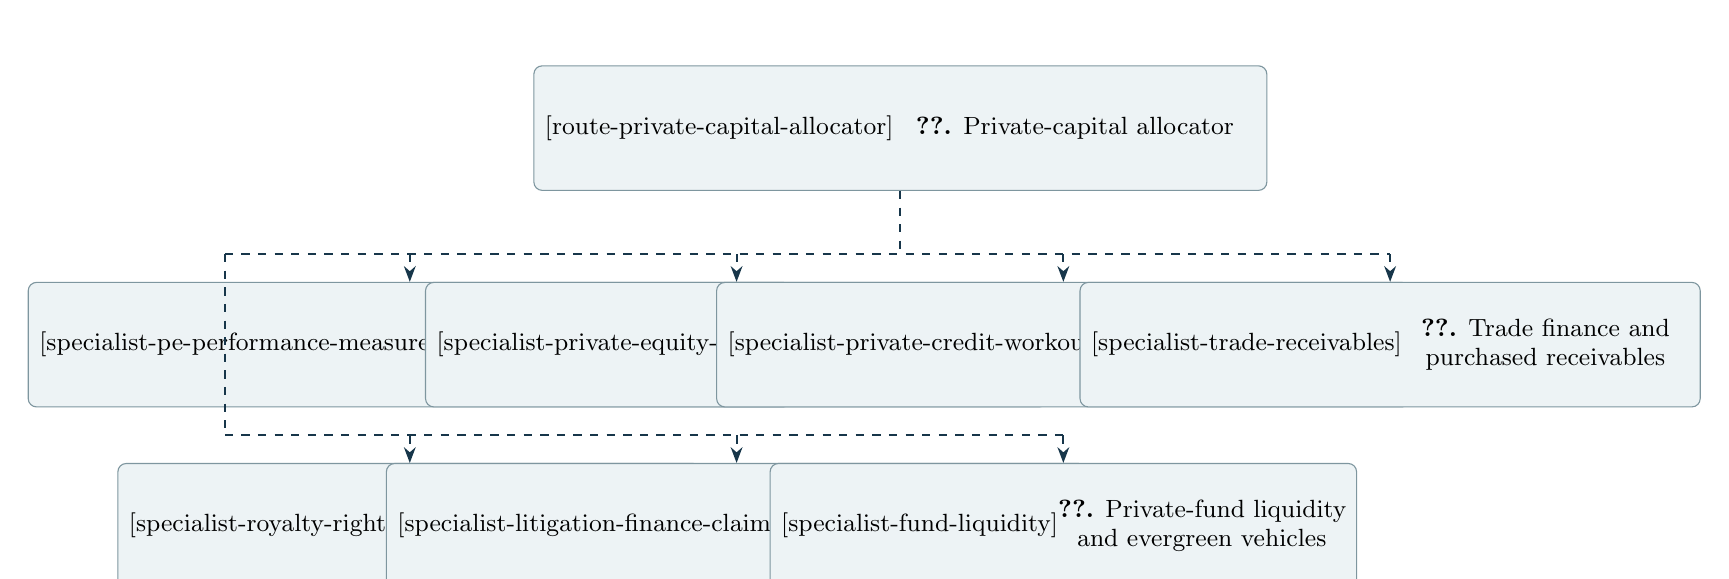
\begin{tikzpicture}[x=1cm,y=1cm]
\node[pathnode] (private-capital-allocator) at (6.23,0) {\MeasurePathNode{4.6cm}{\textbf{\ref*{route-private-capital-allocator}.} Private-capital allocator}\hyperref[route-private-capital-allocator]{\parbox[c][\pathnodeheight][c]{4.6cm}{\centering \textbf{\ref*{route-private-capital-allocator}.} Private-capital allocator}}};
\node[pathnode] (pe-performance-measurement) at (0.00,-2.75) {\MeasurePathNode{3.65cm}{\textbf{\ref*{specialist-pe-performance-measurement}.} PE measurement and replication}\hyperref[specialist-pe-performance-measurement]{\parbox[c][\pathnodeheight][c]{3.65cm}{\centering \textbf{\ref*{specialist-pe-performance-measurement}.} PE measurement and replication}}};
\node[pathnode] (private-equity-vc) at (4.15,-2.75) {\MeasurePathNode{3.65cm}{\textbf{\ref*{specialist-private-equity-vc}.} Private equity and venture security design}\hyperref[specialist-private-equity-vc]{\parbox[c][\pathnodeheight][c]{3.65cm}{\centering \textbf{\ref*{specialist-private-equity-vc}.} Private equity and venture security design}}};
\node[pathnode] (private-credit-workouts) at (8.30,-2.75) {\MeasurePathNode{3.65cm}{\textbf{\ref*{specialist-private-credit-workouts}.} Private credit and workouts}\hyperref[specialist-private-credit-workouts]{\parbox[c][\pathnodeheight][c]{3.65cm}{\centering \textbf{\ref*{specialist-private-credit-workouts}.} Private credit and workouts}}};
\node[pathnode] (trade-receivables) at (12.45,-2.75) {\MeasurePathNode{3.65cm}{\textbf{\ref*{specialist-trade-receivables}.} Trade finance and purchased receivables}\hyperref[specialist-trade-receivables]{\parbox[c][\pathnodeheight][c]{3.65cm}{\centering \textbf{\ref*{specialist-trade-receivables}.} Trade finance and purchased receivables}}};
\node[pathnode] (royalty-rights) at (0.00,-5.05) {\MeasurePathNode{3.65cm}{\textbf{\ref*{specialist-royalty-rights}.} Music and pharmaceutical royalties}\hyperref[specialist-royalty-rights]{\parbox[c][\pathnodeheight][c]{3.65cm}{\centering \textbf{\ref*{specialist-royalty-rights}.} Music and pharmaceutical royalties}}};
\node[pathnode] (litigation-finance-claims) at (4.15,-5.05) {\MeasurePathNode{3.65cm}{\textbf{\ref*{specialist-litigation-finance-claims}.} Litigation claims and legal-finance cash flows}\hyperref[specialist-litigation-finance-claims]{\parbox[c][\pathnodeheight][c]{3.65cm}{\centering \textbf{\ref*{specialist-litigation-finance-claims}.} Litigation claims and legal-finance cash flows}}};
\node[pathnode] (fund-liquidity) at (8.30,-5.05) {\MeasurePathNode{3.65cm}{\textbf{\ref*{specialist-fund-liquidity}.} Private-fund liquidity and evergreen vehicles}\hyperref[specialist-fund-liquidity]{\parbox[c][\pathnodeheight][c]{3.65cm}{\centering \textbf{\ref*{specialist-fund-liquidity}.} Private-fund liquidity and evergreen vehicles}}};
\draw[entryline] (private-capital-allocator.south) -- (6.23,-1.60);
\draw[entryline] (-2.35,-1.60) -- (-2.35,-3.90);
\draw[entryline] (-2.35,-1.60) -- (12.45,-1.60);
\draw[entryarrow] (0.00,-1.60) -- (pe-performance-measurement.north);
\draw[entryarrow] (4.15,-1.60) -- (private-equity-vc.north);
\draw[entryarrow] (8.30,-1.60) -- (private-credit-workouts.north);
\draw[entryarrow] (12.45,-1.60) -- (trade-receivables.north);
\draw[entryline] (-2.35,-3.90) -- (8.30,-3.90);
\draw[entryarrow] (0.00,-3.90) -- (royalty-rights.north);
\draw[entryarrow] (4.15,-3.90) -- (litigation-finance-claims.north);
\draw[entryarrow] (8.30,-3.90) -- (fund-liquidity.north);
\end{tikzpicture}\end{center}
\textbf{Bring these foundations with you.}\begin{itemize}
\item \hyperref[specialist-performance-manager-evaluation]{Performance attribution and manager evaluation} --- needed by \hyperref[specialist-pe-performance-measurement]{PE measurement and replication}.
\item \hyperref[specialist-corporate-credit-cds]{Corporate bonds and credit derivatives} --- needed by \hyperref[specialist-private-credit-workouts]{Private credit and workouts}.
\end{itemize}\hyperref[learning-map]{Return to the whole-guide DAG.}
\Needspace{12\baselineskip}
\subsection{Private-market performance measurement and replication}\label{specialist-pe-performance-measurement}
\textbf{Specialist pathway.} In \hyperref[route-private-capital-allocator]{Private-capital allocator}.

\textbf{Outcome.} Measure private-fund performance with PME, direct alpha and cash-flow-based returns, and test whether public replication explains it.

\textbf{Prerequisites.} Private-capital overview; performance attribution.

\textbf{Review first.} \hyperref[route-private-capital-allocator]{Private-capital allocator}; \hyperref[specialist-performance-manager-evaluation]{Performance attribution and manager evaluation}.

\textbf{Required readings, in order}
\begin{enumerate}\raggedright
\Needspace{5\baselineskip}\item \href{institutional_quantitative_finance_reading_list.pdf\#wide-kaplan-sensoy-survey}{Steven N. Kaplan and Berk A. Sensoy, ``Private Equity Performance: A Survey''}\CataloguePage{404}\NoteKey{wide-kaplan-sensoy-survey}\par \textbf{Foundations.} Survey PE performance evidence.
\Needspace{5\baselineskip}\item \href{institutional_quantitative_finance_reading_list.pdf\#wide-korteweg-risk-adj}{Arthur Korteweg, ``Risk Adjustment in Private Equity Returns''}\CataloguePage{404}\NoteKey{wide-korteweg-risk-adj}\par \textbf{Foundations.} Review risk-adjustment methods.
\Needspace{5\baselineskip}\item \href{institutional_quantitative_finance_reading_list.pdf\#wide-sorensen-jagannathan-pme}{Morten Sorensen and Ravi Jagannathan, ``The Public Market Equivalent and Private Equity Performance''}\CataloguePage{404}\NoteKey{wide-sorensen-jagannathan-pme}\par \textbf{Theory.} Justify PME as an SDF measure.
\Needspace{5\baselineskip}\item \href{institutional_quantitative_finance_reading_list.pdf\#wide-gredil-direct-alpha}{Oleg R. Gredil, Barry Griffiths and Rüdiger Stucke, ``Benchmarking private equity: The Direct Alpha method''}\CataloguePage{404}\NoteKey{wide-gredil-direct-alpha}\par \textbf{Methods.} Compute direct alpha.
\Needspace{5\baselineskip}\item \href{institutional_quantitative_finance_reading_list.pdf\#wide-ang-chen-goetzmann-phalippou}{Andrew Ang, Bingxu Chen, William N. Goetzmann and Ludovic Phalippou, ``Estimating Private Equity Returns from Limited Partner Cash Flows''}\CataloguePage{404}\NoteKey{wide-ang-chen-goetzmann-phalippou}\par \textbf{Methods.} Estimate a PE return series from cash flows.
\Needspace{5\baselineskip}\item \href{institutional_quantitative_finance_reading_list.pdf\#wide-brown-ghysels-gredil}{Gregory W. Brown, Eric Ghysels and Oleg R. Gredil, ``Nowcasting Net Asset Values: The Case of Private Equity''}\CataloguePage{404}\NoteKey{wide-brown-ghysels-gredil}\par \textbf{Methods.} Nowcast NAVs from public data.
\Needspace{5\baselineskip}\item \href{institutional_quantitative_finance_reading_list.pdf\#wide-getmansky-lo-makarov}{Mila Getmansky, Andrew W. Lo and Igor Makarov, ``An econometric model of serial correlation and illiquidity in hedge fund returns''}\CataloguePage{109}\NoteKey{wide-getmansky-lo-makarov}\par \textbf{Methods.} Unsmooth reported returns.
\Needspace{5\baselineskip}\item \href{institutional_quantitative_finance_reading_list.pdf\#wide-gupta-vn-strips}{Arpit Gupta and Stijn Van Nieuwerburgh, ``Valuing Private Equity Investments Strip by Strip''}\CataloguePage{405}\NoteKey{wide-gupta-vn-strips}\par \textbf{Valuation.} Value fund cash flows strip by strip.
\Needspace{5\baselineskip}\item \href{institutional_quantitative_finance_reading_list.pdf\#wide-stafford-replicating-pe}{Erik Stafford, ``Replicating Private Equity with Value Investing, Homemade Leverage, and Hold-to-Maturity Accounting''}\CataloguePage{405}\NoteKey{wide-stafford-replicating-pe}\par \textbf{Counter-evidence.} Replicate buyouts with levered small value.
\Needspace{5\baselineskip}\item \href{institutional_quantitative_finance_reading_list.pdf\#wide-phalippou-fees}{Ludovic Phalippou, Christian Rauch and Marc Umber, ``Private equity portfolio company fees''}\CataloguePage{405}\NoteKey{wide-phalippou-fees}\par \textbf{Evidence.} Account for portfolio-company fees.
\Needspace{5\baselineskip}\item \href{institutional_quantitative_finance_reading_list.pdf\#latest-ercan-private-equity-marks-2025}{Ege Y. Ercan, Steven N. Kaplan and Ilya A. Strebulaev, Interim Valuations, Predictability, and Outcomes in Private Equity}\CataloguePage{403}\NoteKey{latest-ercan-private-equity-marks-2025}\par \textbf{Evidence.} Test what interim marks predict.
\Needspace{5\baselineskip}\item \href{institutional_quantitative_finance_reading_list.pdf\#w4-phalippou-tyranny-irr}{Ludovic Phalippou, ``The Tyranny of IRR''}\CataloguePage{405}\NoteKey{w4-phalippou-tyranny-irr}\par \textbf{Counter-evidence.} See why since-inception IRR misstates wealth growth.
\end{enumerate}
\Needspace{5\baselineskip}\textbf{Checkpoint.} For a set of fund cash flows, compute IRR, TVPI, KS-PME and direct alpha against two benchmarks; estimate an unsmoothed return series, compare with a levered small-value replication, and report fee drag and the dependence of conclusions on benchmark choice.

\textbf{Optional branches.} \href{institutional_quantitative_finance_reading_list.pdf\#wide-phalippou-laid-bare}{Read a critical guide to PE fund economics.}\BranchPage{405} \href{institutional_quantitative_finance_reading_list.pdf\#wide-cochrane-vc}{Estimate VC risk with selection correction.}\BranchPage{405} \href{institutional_quantitative_finance_reading_list.pdf\#w3-goyal-wahal-yavuz-partners}{Study manager selection in private markets.}\BranchPage{405} \href{institutional_quantitative_finance_reading_list.pdf\#w4-cao-vanbeek-private-cashflows}{Model private-fund cash flows with latent factors.}\BranchPage{410}
\par{\small \hyperref[learning-map]{Learning pathway DAG} \textbar{} \hyperref[route-private-capital-allocator]{Section overview} \textbar{} \hyperref[map-private-capital-allocator]{Section DAG}\NoteKey{pe-performance-measurement}}
\Needspace{12\baselineskip}
\subsection{Private equity and venture security design}\label{specialist-private-equity-vc}
\textbf{Specialist pathway.} In \hyperref[route-private-capital-allocator]{Private-capital allocator}.

\textbf{Outcome.} Connect deal cash flows, preferred security rights and fund-level performance measures.

\textbf{Prerequisites.} Private-capital allocator; discounted cash flow and capitalisation tables.

\textbf{Review first.} \hyperref[route-private-capital-allocator]{Private-capital allocator}.

\textbf{Required readings, in order}
\begin{enumerate}\raggedright
\Needspace{5\baselineskip}\item \href{institutional_quantitative_finance_reading_list.pdf\#depth-pe-rosenbaum-pearl-lbo}{Joshua Rosenbaum and Joshua Pearl, \emph{Investment Banking: Valuation, LBOs, M\&A, and IPOs} (3rd ed.)}\CataloguePage{406}\NoteKey{depth-pe-rosenbaum-pearl-lbo}\par \textbf{Valuation.} Build a leveraged-buyout operating and debt model.
\Needspace{5\baselineskip}\item \href{institutional_quantitative_finance_reading_list.pdf\#depth-vc-kaplan-stromberg-contracts}{Steven N. Kaplan and Per Str\"omberg, Financial Contracting Theory Meets the Real World: An Empirical Analysis of Venture Capital Contracts}\CataloguePage{407}\NoteKey{depth-vc-kaplan-stromberg-contracts}\par \textbf{Mechanics.} Read VC control, cash-flow and liquidation rights.
\Needspace{5\baselineskip}\item \href{institutional_quantitative_finance_reading_list.pdf\#depth-vc-yc-safe}{Y Combinator, Post-money SAFE forms and user guide}\CataloguePage{407}\NoteKey{depth-vc-yc-safe}\par \textbf{Mechanics.} Work conversion and dilution through a current SAFE form.
\Needspace{5\baselineskip}\item \href{institutional_quantitative_finance_reading_list.pdf\#pe-gornall-strebulaev-2020}{Will Gornall and Ilya A. Strebulaev, Squaring Venture Capital Valuations with Reality}\CataloguePage{403}\NoteKey{pe-gornall-strebulaev-2020}\par \textbf{Valuation.} Value a private-company security with preference stacks.
\Needspace{5\baselineskip}\item \href{institutional_quantitative_finance_reading_list.pdf\#pe-kaplan-schoar-2005}{Steven N. Kaplan and Antoinette Schoar, Private Equity Performance: Returns, Persistence, and Capital Flows}\CataloguePage{402}\NoteKey{pe-kaplan-schoar-2005}\par \textbf{Evidence.} Understand persistence and benchmark choices in fund returns.
\Needspace{5\baselineskip}\item \href{institutional_quantitative_finance_reading_list.pdf\#pe-korteweg-sorensen-2017}{Arthur Korteweg and Morten Sørensen, Skill and Luck in Private Equity Performance; Version of record DOI}\CataloguePage{402}\NoteKey{pe-korteweg-sorensen-2017}\par \textbf{Evidence.} Account for selection and risk in private-fund performance.
\Needspace{5\baselineskip}\item \href{institutional_quantitative_finance_reading_list.pdf\#pe-ilpa-performance-2025}{Institutional Limited Partners Association (ILPA), ILPA Performance Template}\CataloguePage{404}\NoteKey{pe-ilpa-performance-2025}\par \textbf{Data.} Use consistent LP-level cash-flow and performance reporting.
\Needspace{5\baselineskip}\item \href{institutional_quantitative_finance_reading_list.pdf\#pe-abuzov-continuations-2025}{Rustam Abuzov, Will Gornall, Sophie Shive, Ilya A. Strebulaev, and Michael S. Weisbach, Selling to Yourself: Continuation Funds in Private Equity}\CataloguePage{403}\NoteKey{pe-abuzov-continuations-2025}\par \textbf{Evidence.} Evaluate continuation vehicles with selection and valuation effects.
\Needspace{5\baselineskip}\item \href{institutional_quantitative_finance_reading_list.pdf\#pe-ilpa-continuation-2023}{Institutional Limited Partners Association (ILPA), Continuation Funds: Considerations for Limited Partners and General Partners; ILPA status of 2026 draft}\CataloguePage{403}\NoteKey{pe-ilpa-continuation-2023}\par \textbf{Implementation.} Assess process and conflict controls around a GP-led exit.
\Needspace{5\baselineskip}\item \href{institutional_quantitative_finance_reading_list.pdf\#latest-ercan-private-equity-marks-2025}{Ege Y. Ercan, Steven N. Kaplan and Ilya A. Strebulaev, Interim Valuations, Predictability, and Outcomes in Private Equity}\CataloguePage{403}\NoteKey{latest-ercan-private-equity-marks-2025}\par \textbf{Valuation evidence.} Relate interim portfolio-company marks to eventual outcomes while accounting for stale marks and selected exits.
\end{enumerate}
\Needspace{5\baselineskip}\textbf{Checkpoint.} Model one LBO and one VC exit waterfall including multiple SAFE or preferred rounds. Calculate gross deal proceeds, LP cash flows, MOIC, IRR and PME at dated valuation marks; compare a sale with a continuation vehicle under fees and conflicts. Use a public or synthetic transaction when executed contracts are unavailable. Separate interim marks from realized proceeds in the cash-flow worksheet.

\textbf{Optional branches.} \href{institutional_quantitative_finance_reading_list.pdf\#wide-gompers-vc-decisions}{Read survey evidence on VC decisions.}\BranchPage{405} \href{institutional_quantitative_finance_reading_list.pdf\#w2-kaplan-lerner-vc}{Read long-run VC industry evidence.}\BranchPage{405} \href{institutional_quantitative_finance_reading_list.pdf\#w2-korteweg-sorensen-vc}{Estimate VC risk and return with selection.}\BranchPage{406} \href{institutional_quantitative_finance_reading_list.pdf\#w2-ewens-diversifiable}{See idiosyncratic risk priced in VC.}\BranchPage{406} \href{institutional_quantitative_finance_reading_list.pdf\#w2-hall-woodward}{Value undiversified entrepreneurial risk.}\BranchPage{406} \href{institutional_quantitative_finance_reading_list.pdf\#w3-kisseleva-selection-early-stage}{Quantify selection bias in early-stage returns.}\BranchPage{406} \href{institutional_quantitative_finance_reading_list.pdf\#w4-hellmann-vc-jcurves}{Relate VC financing capacity to start-up J-curves.}\BranchPage{406} \href{institutional_quantitative_finance_reading_list.pdf\#w5-axelson-borrow-cheap}{Relate buyout leverage to credit conditions.}\BranchPage{408} \href{institutional_quantitative_finance_reading_list.pdf\#w5-gompers-kaplan-mukharlyamov}{See how PE firms actually value deals.}\BranchPage{408}
\par{\small \hyperref[learning-map]{Learning pathway DAG} \textbar{} \hyperref[route-private-capital-allocator]{Section overview} \textbar{} \hyperref[map-private-capital-allocator]{Section DAG}\NoteKey{private-equity-vc}}
\Needspace{12\baselineskip}
\subsection{Private credit and workouts}\label{specialist-private-credit-workouts}
\textbf{Specialist pathway.} In \hyperref[route-private-capital-allocator]{Private-capital allocator}.

\textbf{Outcome.} Underwrite direct loans by covenant, collateral, valuation and restructuring waterfall.

\textbf{Prerequisites.} Corporate bonds and credit derivatives; leveraged-finance accounting and legal priority.

\textbf{Review first.} \hyperref[route-private-capital-allocator]{Private-capital allocator}; \hyperref[specialist-corporate-credit-cds]{Corporate bonds and credit derivatives}.

\textbf{Required readings, in order}
\begin{enumerate}\raggedright
\Needspace{5\baselineskip}\item \href{institutional_quantitative_finance_reading_list.pdf\#pc-chernenko-erel-prilmeier-2022}{Sergey Chernenko, Isil Erel, and Robert Prilmeier, Why Do Firms Borrow Directly from Nonbanks?}\CataloguePage{410}\NoteKey{pc-chernenko-erel-prilmeier-2022}\par \textbf{Evidence.} Establish the direct-lending market and borrower selection evidence.
\Needspace{5\baselineskip}\item \href{institutional_quantitative_finance_reading_list.pdf\#pc-block-survey-2024}{Joern Block, Young Soo Jang, Steven N. Kaplan, and Anna Schulze, A Survey of Private Debt Funds; Earlier working paper}\CataloguePage{411}\NoteKey{pc-block-survey-2024}\par \textbf{Evidence.} Compare lender structure and loan terms across the market.
\Needspace{5\baselineskip}\item \href{institutional_quantitative_finance_reading_list.pdf\#depth-pc-unitranche-aal-2025}{Simeon Brown, Jessica Ann Rissmiller, Michael Graziano and Heather Sonnenberg, Unitranche Harmony: A 101 on the Agreement Among Lenders}\CataloguePage{413}\NoteKey{depth-pc-unitranche-aal-2025}\par \textbf{Mechanics.} Read unitranche and agreement-among-lenders payment rights.
\Needspace{5\baselineskip}\item \href{institutional_quantitative_finance_reading_list.pdf\#gap-credit-weak-covenants}{Victoria Ivashina and Boris Vallée, Weak Credit Covenants}\CataloguePage{244}\NoteKey{gap-credit-weak-covenants}\par \textbf{Mechanics.} Test carve-outs and deductibles inside headline covenants.
\Needspace{5\baselineskip}\item \href{institutional_quantitative_finance_reading_list.pdf\#pc-ipev-2025}{International Private Equity and Venture Capital Valuation (IPEV) Board, International Private Equity and Venture Capital Valuation Guidelines}\CataloguePage{412}\NoteKey{pc-ipev-2025}\par \textbf{Valuation.} Mark illiquid loans with observable inputs and calibrated uncertainty.
\Needspace{5\baselineskip}\item \href{institutional_quantitative_finance_reading_list.pdf\#pc-sp-defaults-2024}{S\&P Global Ratings, Private Credit Payment Defaults Rose in 2023 as Weaker Borrowers Struggled to Service Debt}\CataloguePage{413}\NoteKey{pc-sp-defaults-2024}\par \textbf{Data.} Use selected default-incidence and exchange-price evidence; obtain ultimate recovery cash flows separately.
\Needspace{5\baselineskip}\item \href{institutional_quantitative_finance_reading_list.pdf\#depth-pc-occ-abl}{Office of the Comptroller of the Currency, \emph{Asset-Based Lending}, Comptroller's Handbook}\CataloguePage{413}\NoteKey{depth-pc-occ-abl}\par \textbf{Mechanics.} Assess borrowing bases, eligibility and advance rates in ABL.
\Needspace{5\baselineskip}\item \href{institutional_quantitative_finance_reading_list.pdf\#evidence-unitranche-aal}{U.S. Well Services lenders, Agreement Among Lenders}\CataloguePage{413}\NoteKey{evidence-unitranche-aal}\par \textbf{Data.} Compare model rights with an executed unitranche example.
\Needspace{5\baselineskip}\item \href{institutional_quantitative_finance_reading_list.pdf\#evidence-serta-workout}{U.S. Court of Appeals for the Fifth Circuit, In re Serta Simmons Bedding, L.L.C.}\CataloguePage{414}\NoteKey{evidence-serta-workout}\par \textbf{Implementation.} Run priming and uptiering outcomes through creditor classes.
\Needspace{5\baselineskip}\item \href{institutional_quantitative_finance_reading_list.pdf\#depth-pc-sp-2025-workouts}{S\&P Global Ratings, Pre-Tariff U.S. Middle-Market Collateralized Loan Obligation Rally Is Unlikely To Last}\CataloguePage{413}\NoteKey{depth-pc-sp-2025-workouts}\par \textbf{Implementation.} Compare observed workouts with par-mark and model assumptions.
\Needspace{5\baselineskip}\item \href{institutional_quantitative_finance_reading_list.pdf\#latest-robinson-wallskog-retail-private-lending-2026}{David T. Robinson and Melanie Wallskog, The Growth of Private Lending and Retail Access to Alternative Investments}\CataloguePage{411}\NoteKey{latest-robinson-wallskog-retail-private-lending-2026}\par \textbf{Investor economics.} Separate listed-BDC investor fees and benchmarks from direct-loan asset returns and other private-fund structures.
\end{enumerate}
\Needspace{5\baselineskip}\textbf{Checkpoint.} Underwrite a public or synthetic unitranche loan with cash interest, PIK, collateral and covenant baskets. Run base, liquidity squeeze and restructuring scenarios through the lender waterfall; reconcile the valuation mark with comparable spreads and the legal rights actually available. State data and side-letter gaps. Add a listed-BDC investor-fee layer and compare its benchmark with the loan-level analysis.

\textbf{Optional branches.} \href{institutional_quantitative_finance_reading_list.pdf\#w2-bostonfed-bdc-pik}{Track payment-in-kind usage in BDC portfolios.}\BranchPage{414} \href{institutional_quantitative_finance_reading_list.pdf\#w2-zou-private-credit-survey}{Read a 2026 survey of private-credit evidence.}\BranchPage{414} \href{institutional_quantitative_finance_reading_list.pdf\#w5-kermani-ma-specificity}{Use liquidation values to anchor recoveries.}\BranchPage{245} \href{institutional_quantitative_finance_reading_list.pdf\#w5-jiang-li-wang-ch11}{See hedge funds' role in Chapter 11.}\BranchPage{245} \href{institutional_quantitative_finance_reading_list.pdf\#w5-schwert-bank-vs-market}{Compare bank-loan and bond pricing.}\BranchPage{245}
\par{\small \hyperref[learning-map]{Learning pathway DAG} \textbar{} \hyperref[route-private-capital-allocator]{Section overview} \textbar{} \hyperref[map-private-capital-allocator]{Section DAG}\NoteKey{private-credit-workouts}}
\Needspace{12\baselineskip}
\subsection{Trade finance and purchased receivables}\label{specialist-trade-receivables}
\textbf{Specialist pathway.} In \hyperref[route-private-capital-allocator]{Private-capital allocator}.

\textbf{Outcome.} Distinguish bank undertakings from purchased invoices and model the seller, debtor, bank and collection risks.

\textbf{Prerequisites.} Private-capital allocator; working capital, credit loss and discounting.

\textbf{Review first.} \hyperref[route-private-capital-allocator]{Private-capital allocator}.

\textbf{Required readings, in order}
\begin{enumerate}\raggedright
\Needspace{5\baselineskip}\item \href{institutional_quantitative_finance_reading_list.pdf\#depth-special-occ-trade-2018}{Office of the Comptroller of the Currency, \emph{Trade Finance and Services}, Comptroller's Handbook}\CataloguePage{414}\NoteKey{depth-special-occ-trade-2018}\par \textbf{Mechanics.} Map letters of credit, guarantees, open-account finance and prepayments to their different obligations.
\Needspace{5\baselineskip}\item \href{institutional_quantitative_finance_reading_list.pdf\#evidence-trade-antras}{Pol Antr\`as and C. Fritz Foley, Poultry in Motion: A Study of International Trade Finance Practices; author-hosted published text}\CataloguePage{414}\NoteKey{evidence-trade-antras}\par \textbf{Empirical evidence.} Study how relationship and enforcement conditions select payment terms in the single-exporter sample.
\Needspace{5\baselineskip}\item \href{institutional_quantitative_finance_reading_list.pdf\#gapclose-trade-factoring-contract}{Majesco / HSBC Bank USA, Receivables Purchase Agreement, Schedule and Standard Terms, Exhibit 10.1}\CataloguePage{415}\NoteKey{gapclose-trade-factoring-contract}\par \textbf{Executed contract.} Translate a negotiated advance, concentration limit, reserve and recourse agreement into cash timing.
\Needspace{5\baselineskip}\item \href{institutional_quantitative_finance_reading_list.pdf\#depth-special-icc-trade-2025}{International Chamber of Commerce, ICC Trade Register: The Global Benchmark for Trade and Supply Chain Finance}\CataloguePage{414}\NoteKey{depth-special-icc-trade-2025}\par \textbf{Data and comparison.} Use product-specific denominators and licensed loss tables if available; do not substitute a headline default rate.
\Needspace{5\baselineskip}\item \href{institutional_quantitative_finance_reading_list.pdf\#depth-pc-occ-abl}{Office of the Comptroller of the Currency, \emph{Asset-Based Lending}, Comptroller's Handbook}\CataloguePage{413}\NoteKey{depth-pc-occ-abl}\par \textbf{Implementation.} Check eligibility, collateral monitoring and borrowing-base controls alongside the purchase agreement.
\Needspace{5\baselineskip}\item \href{institutional_quantitative_finance_reading_list.pdf\#w6-petersen-rajan-trade-credit}{Mitchell A. Petersen and Raghuram G. Rajan, ``Trade Credit: Theories and Evidence''}\CataloguePage{417}\NoteKey{w6-petersen-rajan-trade-credit}\par \textbf{Foundations.} Learn why firms extend and use trade credit.
\end{enumerate}
\Needspace{5\baselineskip}\textbf{Checkpoint.} For one illustrative invoice, compute seller proceeds, advance interest, fees, reserve release and factor exposure using the disclosed historical contract. Run debtor delay, dispute, dilution and default branches, retaining seller recourse. Keep its historical reference rate explicit. Compare the structure with a letter of credit and identify which licensed or private collection data would be required to estimate portfolio net returns.

\textbf{Optional branches.} \href{institutional_quantitative_finance_reading_list.pdf\#w6-klapper-factoring}{See factoring substitute for weak creditor rights.}\BranchPage{417} \href{institutional_quantitative_finance_reading_list.pdf\#w6-murfin-njoroge}{Measure costs of stretched payables.}\BranchPage{417} \href{institutional_quantitative_finance_reading_list.pdf\#w6-barrot-trade-credit}{See payment terms act as entry barriers.}\BranchPage{417} \href{institutional_quantitative_finance_reading_list.pdf\#w6-amberg-trade-credit}{Trace liquidity shocks through trade credit.}\BranchPage{417}
\par{\small \hyperref[learning-map]{Learning pathway DAG} \textbar{} \hyperref[route-private-capital-allocator]{Section overview} \textbar{} \hyperref[map-private-capital-allocator]{Section DAG}\NoteKey{trade-receivables}}
\Needspace{12\baselineskip}
\subsection{Music and pharmaceutical royalties}\label{specialist-royalty-rights}
\textbf{Specialist pathway.} In \hyperref[route-private-capital-allocator]{Private-capital allocator}.

\textbf{Outcome.} Value a precisely defined royalty interest through sales, rights, contract amendments and collection risk.

\textbf{Prerequisites.} Private-capital allocator; product cash-flow forecasting, IP rights and accounting.

\textbf{Review first.} \hyperref[route-private-capital-allocator]{Private-capital allocator}.

\textbf{Required readings, in order}
\begin{enumerate}\raggedright
\Needspace{5\baselineskip}\item \href{institutional_quantitative_finance_reading_list.pdf\#depth-special-wipo-music-2026}{Peter Tschmuck, Dennis Collopy and Christian Handke, IP Finance in the Music Industry}\CataloguePage{416}\NoteKey{depth-special-wipo-music-2026}\par \textbf{Rights and mechanics.} Distinguish music rights, revenue channels and financing structures before defining the purchased claim.
\Needspace{5\baselineskip}\item \href{institutional_quantitative_finance_reading_list.pdf\#evidence-pharma-royalties}{Royalty Pharma, 2025 Form 10-K; 30 June 2026 Form 10-Q}\CataloguePage{416}\NoteKey{evidence-pharma-royalties}\par \textbf{Valuation and accounts.} Separate marketed royalties, development finance, milestones, accounting values and corporate costs.
\Needspace{5\baselineskip}\item \href{institutional_quantitative_finance_reading_list.pdf\#gapclose-pharma-royalty-contract}{PTC Therapeutics / Royalty Pharma, 2023 amended royalty purchase agreement; signed 2025 Amendment No. 2; June 2026 filing}\CataloguePage{416}\NoteKey{gapclose-pharma-royalty-contract}\par \textbf{Executed contract and amendments.} Track the dated seller/buyer split, payment cap, full transfer and contingent purchase payments.
\Needspace{5\baselineskip}\item \href{institutional_quantitative_finance_reading_list.pdf\#gap-damodaran4}{Aswath Damodaran, Investment Valuation: Tools and Techniques for Determining the Value of Any Asset}\CataloguePage{199}\NoteKey{gap-damodaran4}\par \textbf{Valuation discipline.} Separate forecast growth, product risk and discount-rate assumptions from contractual ownership percentages.
\Needspace{5\baselineskip}\item \href{institutional_quantitative_finance_reading_list.pdf\#w6-fernandez-stein-lo-royalty}{Jose-Maria Fernandez, Roger M. Stein and Andrew W. Lo, ``Commercializing biomedical research through securitization techniques''}\CataloguePage{418}\NoteKey{w6-fernandez-stein-lo-royalty}\par \textbf{Financing.} See how pooled drug royalties and projects can be tranched and securitised.
\end{enumerate}
\Needspace{5\baselineskip}\textbf{Checkpoint.} Construct separate 2023 and post-December-2025 Evrysdi royalty waterfalls using the inspected clauses. Bridge product sales to the assigned royalty, purchaser receipts, contingent acquisition payments and issuer accounting. Stress sales decline, patent/licence interruption and payer default without inventing redacted terms. Contrast the claim with music-rights revenue allocation. Report scenario values, not investor realised returns, unless acquisition, collection, fee and tax cash flows reconcile.

\par{\small \hyperref[learning-map]{Learning pathway DAG} \textbar{} \hyperref[route-private-capital-allocator]{Section overview} \textbar{} \hyperref[map-private-capital-allocator]{Section DAG}\NoteKey{royalty-rights}}
\Needspace{12\baselineskip}
\subsection{Litigation claims and legal-finance cash flows}\label{specialist-litigation-finance-claims}
\textbf{Specialist pathway.} In \hyperref[route-private-capital-allocator]{Private-capital allocator}.

\textbf{Outcome.} Underwrite a claim-linked payoff as a contingent multi-stage cash flow while separating consumer evidence, commercial claims, legal restrictions and investor-level net returns.

\textbf{Prerequisites.} Private-capital allocator; discounted cash flow, probability trees and private-asset reporting.

\textbf{Review first.} \hyperref[route-private-capital-allocator]{Private-capital allocator}.

\textbf{Required readings, in order}
\begin{enumerate}\raggedright
\Needspace{5\baselineskip}\item \href{institutional_quantitative_finance_reading_list.pdf\#depth-special-gao-litigation-2023}{U.S. Government Accountability Office, Third-Party Litigation Financing: Market Characteristics, Data, and Trends}\CataloguePage{416}\NoteKey{depth-special-gao-litigation-2023}\par \textbf{Mechanics.} Separate consumer legal funding from commercial litigation finance and identify disclosure/data gaps.
\Needspace{5\baselineskip}\item \href{institutional_quantitative_finance_reading_list.pdf\#evidence-litigation-study}{Ronen Avraham and Anthony Sebok, An Empirical Investigation of Third Party Consumer Litigant Funding; journal full text}\CataloguePage{416}\NoteKey{evidence-litigation-study}\par \textbf{Evidence.} Use observed consumer applications, fees and collections only within its study population.
\Needspace{5\baselineskip}\item \href{institutional_quantitative_finance_reading_list.pdf\#gap-damodaran4}{Aswath Damodaran, Investment Valuation: Tools and Techniques for Determining the Value of Any Asset}\CataloguePage{199}\NoteKey{gap-damodaran4}\par\emph{Selection:} Decision-tree and contingent-claim valuation topics.\par \textbf{Valuation.} Build scenario-valued contingent cash flows with explicit probabilities and discount rates.
\Needspace{5\baselineskip}\item \href{institutional_quantitative_finance_reading_list.pdf\#pe-ilpa-performance-2025}{Institutional Limited Partners Association (ILPA), ILPA Performance Template}\CataloguePage{404}\NoteKey{pe-ilpa-performance-2025}\par \textbf{Implementation.} Specify gross-to-net fees, expenses and investor cash-flow reporting requirements for any portfolio claim.
\end{enumerate}
\Needspace{5\baselineskip}\textbf{Checkpoint.} Build a stylized single-claim decision tree from filing through settlement, trial, appeal and actual collection, with legal cost, duration, adverse-cost and funding waterfall scenarios. Show the investor payoff for win, partial recovery and loss, then a sensitivity grid for probability, delay and fees. Label study-derived versus assumed parameters; do not present a fund IRR or executed agreement term unless those source documents are available.

\textbf{Optional branches.} \href{institutional_quantitative_finance_reading_list.pdf\#pc-erel-flanagan-weisbach-2024}{Compare risk-adjusted private-debt return methods without treating litigation claims as conventional loans.}\BranchPage{411} \href{institutional_quantitative_finance_reading_list.pdf\#pe-kaplan-schoar-2005}{Use cash-flow-aware private-investment performance concepts, while marking their non-transferability to one unobserved claim.}\BranchPage{402} \href{institutional_quantitative_finance_reading_list.pdf\#w6-abrams-chen-litigation}{Read funder-level evidence on case returns.}\BranchPage{418}
\par{\small \hyperref[learning-map]{Learning pathway DAG} \textbar{} \hyperref[route-private-capital-allocator]{Section overview} \textbar{} \hyperref[map-private-capital-allocator]{Section DAG}\NoteKey{litigation-finance-claims}}
\Needspace{12\baselineskip}
\subsection{Private-fund liquidity and evergreen vehicles}\label{specialist-fund-liquidity}
\textbf{Specialist pathway.} In \hyperref[route-private-capital-allocator]{Private-capital allocator}.

\textbf{Outcome.} Model capital calls, NAV leverage and periodic redemptions as contingent cash-flow claims.

\textbf{Prerequisites.} Private-capital allocator; fund accounting and LP cash-flow measures.

\textbf{Review first.} \hyperref[route-private-capital-allocator]{Private-capital allocator}.

\textbf{Required readings, in order}
\begin{enumerate}\raggedright
\Needspace{5\baselineskip}\item \href{institutional_quantitative_finance_reading_list.pdf\#depth-pe-takahashi-alexander-2002}{Dean Takahashi and Seth Alexander, Illiquid Alternative Asset Fund Modeling}\CataloguePage{408}\NoteKey{depth-pe-takahashi-alexander-2002}\par \textbf{Valuation.} Model commitment, drawdown and distribution paths.
\Needspace{5\baselineskip}\item \href{institutional_quantitative_finance_reading_list.pdf\#depth-pe-robinson-sensoy-cashflows}{David T. Robinson and Berk A. Sensoy, Cyclicality, Performance Measurement, and Cash Flow Liquidity in Private Equity}\CataloguePage{409}\NoteKey{depth-pe-robinson-sensoy-cashflows}\par \textbf{Evidence.} Compare actual private-fund cash-flow timing with simplified J-curves.
\Needspace{5\baselineskip}\item \href{institutional_quantitative_finance_reading_list.pdf\#depth-pe-ilpa-subline-2020}{Institutional Limited Partners Association, Guidance on Enhancing Transparency Around Subscription Lines of Credit}\CataloguePage{409}\NoteKey{depth-pe-ilpa-subline-2020}\par \textbf{Mechanics.} Separate investment return from subscription-line timing effects.
\Needspace{5\baselineskip}\item \href{institutional_quantitative_finance_reading_list.pdf\#depth-pe-ilpa-nav-2024}{Institutional Limited Partners Association, NAV-Based Facilities Guidance \& Roadmap}\CataloguePage{409}\NoteKey{depth-pe-ilpa-nav-2024}\par \textbf{Mechanics.} Read NAV financing disclosure and LP risk allocation.
\Needspace{5\baselineskip}\item \href{institutional_quantitative_finance_reading_list.pdf\#evidence-hvpe-nav}{HarbourVest Global Private Equity, Annual Report and Accounts 2025}\CataloguePage{409}\NoteKey{evidence-hvpe-nav}\par \textbf{Data.} Trace a listed fund's cash and leverage in an actual report.
\Needspace{5\baselineskip}\item \href{institutional_quantitative_finance_reading_list.pdf\#add-interval-mechanics}{U.S. Securities and Exchange Commission, Investor Bulletin: Interval Funds}\CataloguePage{411}\NoteKey{add-interval-mechanics}\par \textbf{Mechanics.} Define repurchase windows, limits, proration and valuation timing.
\Needspace{5\baselineskip}\item \href{institutional_quantitative_finance_reading_list.pdf\#add-interval-evidence}{I. Aldasoro, S. Doerr and K. Todorov, Retail Investors in Private Credit}\CataloguePage{411}\NoteKey{add-interval-evidence}\par \textbf{Evidence.} Distinguish BDC and ETF secondary-price evidence from interval-fund repurchase mechanics.
\Needspace{5\baselineskip}\item \href{institutional_quantitative_finance_reading_list.pdf\#add-interval-proposal}{U.S. Securities and Exchange Commission, Interval Fund Modernization and Multiple Share Classes for Registered Closed-End Funds and BDCs}\CataloguePage{412}\NoteKey{add-interval-proposal}\par \textbf{Evidence.} Identify the proposed 2026 SEC changes without treating them as enacted.
\Needspace{5\baselineskip}\item \href{institutional_quantitative_finance_reading_list.pdf\#depth-pe-ilpa-continuation-template-2026}{Institutional Limited Partners Association, Continuation Fund Disclosure Template; ILPA/Coller mock multi-asset and single-asset disclosures}\CataloguePage{410}\NoteKey{depth-pe-ilpa-continuation-template-2026}\par \textbf{Implementation.} Test exit elections and liquidity alternatives in a GP-led event.
\Needspace{5\baselineskip}\item \href{institutional_quantitative_finance_reading_list.pdf\#followup-odyssey-election}{Odyssey Investment Partners, Project Lightning election/transaction materials, in the Golden Gate Transit--Amalgamated Retirement Plan's 21 November 2025 packet}\CataloguePage{410}\NoteKey{followup-odyssey-election}\par \textbf{Data.} Review an actual election notice and the limits of investor choice.
\end{enumerate}
\Needspace{5\baselineskip}\textbf{Checkpoint.} Build separate 24-month cash ledgers for a conventional drawdown LP interest and an interval-fund investment holding comparable credit exposures. For the first, stress calls, distributions and fund-level borrowing; for the second, use the selected prospectus to apply NAV timing, declared repurchase capacity, proration and permitted suspension terms. Compare investor cash shortfalls, fees and return measures without assuming the two vehicles share exit rights. Identify any unavailable loan or fund disclosures.

\textbf{Optional branches.} \href{institutional_quantitative_finance_reading_list.pdf\#wide-jin-swing-pricing}{Evaluate swing pricing as a run deterrent.}\BranchPage{115} \href{institutional_quantitative_finance_reading_list.pdf\#w4-baz-liquidity-premium-models}{Compare three models of the illiquidity premium.}\BranchPage{410}
\par{\small \hyperref[learning-map]{Learning pathway DAG} \textbar{} \hyperref[route-private-capital-allocator]{Section overview} \textbar{} \hyperref[map-private-capital-allocator]{Section DAG}\NoteKey{fund-liquidity}}
\clearpage
\section{Real-asset investor}\label{route-real-asset-investor}
\label{route-13}
\textbf{Learning sequence.} Begin with property and infrastructure valuation, then examine leased equipment, resource rights and collectibles.

\textbf{Section goals.} Across its pathways, this section teaches you to:
\begin{itemize}[leftmargin=1.4em,itemsep=0pt,topsep=1pt]
\item reconcile property values with private indices and listed REIT returns (\hyperref[specialist-property-valuation]{\ref*{specialist-property-valuation}})
\item price contracted and regulated infrastructure cash flows (\hyperref[specialist-infrastructure-regulated-assets]{\ref*{specialist-infrastructure-regulated-assets}})
\item underwrite equipment and aircraft leases (\hyperref[specialist-equipment-aircraft-leasing]{\ref*{specialist-equipment-aircraft-leasing}})
\item value timber, farmland, mineral and water rights (\hyperref[specialist-natural-resource-rights]{\ref*{specialist-natural-resource-rights}})
\item evaluate collectibles from transaction evidence (\hyperref[specialist-collectibles-valuation]{\ref*{specialist-collectibles-valuation}})
\end{itemize}
\textbf{Overview outcome.} Underwrite contracted, regulated, biological and merchant cash flows with their distinct operating and refinancing risks.

\textbf{Prerequisites.} Common toolkit; discounted cash flows, debt service, property income and basic commodity forwards.

\textbf{Review first.} \hyperref[route-common-toolkit]{Common toolkit}.

\textbf{Required readings, in order}
\begin{enumerate}\raggedright
\Needspace{5\baselineskip}\item \href{institutional_quantitative_finance_reading_list.pdf\#depth-geltner-book-2026}{David M. Geltner, Norman G. Miller, Alex Van De Minne, Piet Eichholtz, Thies Lindenthal and Lily Shen, Commercial Real Estate Analysis for Investment, Finance, and Development}\CataloguePage{419}\NoteKey{depth-geltner-book-2026}\par\emph{Selection:} Print chapter 4 (discounted cash flow) and chapter 10 (leases), fourth edition (2026).\par Establish property-level valuation, leasing cash flows and real-estate financing.
\Needspace{5\baselineskip}\item \href{institutional_quantitative_finance_reading_list.pdf\#re-ncreif-npi}{National Council of Real Estate Investment Fiduciaries (NCREIF), NCREIF Property Index (NPI): Index Methodology and FAQs}\CataloguePage{419}\NoteKey{re-ncreif-npi}\par Check what an appraised property index measures and omits before benchmarking a deal.
\Needspace{5\baselineskip}\item \href{institutional_quantitative_finance_reading_list.pdf\#infra-gatti-2023}{Stefano Gatti, Project Finance in Theory and Practice: Designing, Structuring, and Financing Private and Public Projects (4th ed.)}\CataloguePage{421}\NoteKey{infra-gatti-2023}\par Structure project cash flows, contracts and debt around construction and operation phases.
\Needspace{5\baselineskip}\item \href{institutional_quantitative_finance_reading_list.pdf\#depth-gihub-ppp-contract-ops}{Global Infrastructure Hub and Turner \& Townsend, PPP Contract Management Reference Tool; full guide}\CataloguePage{423}\NoteKey{depth-gihub-ppp-contract-ops}\par Trace concession obligations, construction handover, performance deductions and refinancing into valuation.
\Needspace{5\baselineskip}\item \href{institutional_quantitative_finance_reading_list.pdf\#infra-andonov-kraussl-rauh-2021}{Aleksandar Andonov; Roman Kräussl; Joshua Rauh, Institutional Investors and Infrastructure Investing}\CataloguePage{421}\NoteKey{infra-andonov-kraussl-rauh-2021}\par Compare infrastructure's reported investor outcomes with claims of stable, diversifying returns.
\Needspace{5\baselineskip}\item \href{institutional_quantitative_finance_reading_list.pdf\#nr-mcintosh-zhang-faustmann-2024}{Michael G. McIntosh and Daowei Zhang, Faustmann Formula and Its Use in Forest Asset Valuation: A Review and a Suggestion}\CataloguePage{423}\NoteKey{nr-mcintosh-zhang-faustmann-2024}\par Value timber rotations and land use as biological and timing decisions.
\Needspace{5\baselineskip}\item \href{institutional_quantitative_finance_reading_list.pdf\#nr-burt-capitalization-1986}{Oscar R. Burt, Econometric Modeling of the Capitalization Formula for Farmland Prices}\CataloguePage{424}\NoteKey{nr-burt-capitalization-1986}\par Connect farmland prices to expected income and capitalization assumptions.
\Needspace{5\baselineskip}\item \href{institutional_quantitative_finance_reading_list.pdf\#physical-secomandi-storage-2010}{Nicola Secomandi, Optimal Commodity Trading with a Capacitated Storage Asset}\CataloguePage{319}\NoteKey{physical-secomandi-storage-2010}\par Add a physical operating option whose value depends on capacity and market spreads.
\end{enumerate}
\Needspace{5\baselineskip}\textbf{Checkpoint.} Prepare a comparable cash-flow map for one property, one concession and one biological or storage asset. Identify contracted and merchant revenue, operating limits, debt and residual value; calculate how a demand shock and a refinancing shock change each equity value.

\textbf{Optional branches.} \href{institutional_quantitative_finance_reading_list.pdf\#section.16.3}{Deepen farmland, timber and biological-asset measurement.}\BranchPage{423} \href{institutional_quantitative_finance_reading_list.pdf\#section.14.1}{Extend to oil, gas, metals, crops and delivery-location options.}\BranchPage{318}
\par\textbf{Continue in this section.} \hyperref[specialist-property-valuation]{Property valuation and listed real estate}; \hyperref[specialist-infrastructure-regulated-assets]{Infrastructure and regulated assets}; \hyperref[specialist-equipment-aircraft-leasing]{Equipment and aircraft leasing}; \hyperref[specialist-natural-resource-rights]{Timber, farmland, mineral and water rights}; \hyperref[specialist-collectibles-valuation]{Collectibles: auction evidence and investable returns}.
\par{\small \hyperref[learning-map]{Learning pathway DAG} \textbar{} \hyperref[map-real-asset-investor]{Section DAG}\NoteKey{real-asset-investor}}
\clearpage
\subsection*{Real-asset investor: pathway DAG}\phantomsection\label{map-real-asset-investor}
\addcontentsline{toc}{subsection}{Real-asset investor: pathway DAG}
Start with the section overview's readings, for orientation. Solid arrows show prerequisites within this section. Dashed connectors identify entry points with no further prerequisite in this section; the linked foundations below still apply. Follow the arrows for dependencies and the subsection numbers for reading order. Every node is clickable.
\begin{center}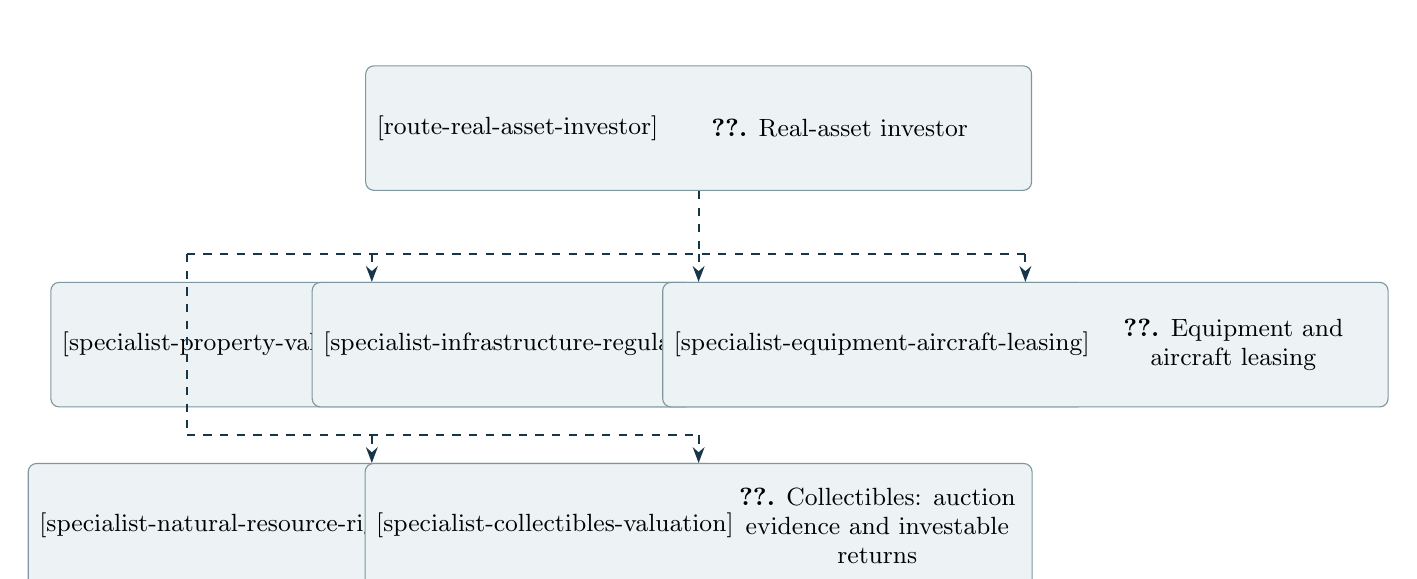
\begin{tikzpicture}[x=1cm,y=1cm]
\node[pathnode] (real-asset-investor) at (4.15,0) {\MeasurePathNode{4.6cm}{\textbf{\ref*{route-real-asset-investor}.} Real-asset investor}\hyperref[route-real-asset-investor]{\parbox[c][\pathnodeheight][c]{4.6cm}{\centering \textbf{\ref*{route-real-asset-investor}.} Real-asset investor}}};
\node[pathnode] (property-valuation) at (0.00,-2.75) {\MeasurePathNode{3.65cm}{\textbf{\ref*{specialist-property-valuation}.} Property valuation and listed real estate}\hyperref[specialist-property-valuation]{\parbox[c][\pathnodeheight][c]{3.65cm}{\centering \textbf{\ref*{specialist-property-valuation}.} Property valuation and listed real estate}}};
\node[pathnode] (infrastructure-regulated-assets) at (4.15,-2.75) {\MeasurePathNode{3.65cm}{\textbf{\ref*{specialist-infrastructure-regulated-assets}.} Infrastructure and regulated assets}\hyperref[specialist-infrastructure-regulated-assets]{\parbox[c][\pathnodeheight][c]{3.65cm}{\centering \textbf{\ref*{specialist-infrastructure-regulated-assets}.} Infrastructure and regulated assets}}};
\node[pathnode] (equipment-aircraft-leasing) at (8.30,-2.75) {\MeasurePathNode{3.65cm}{\textbf{\ref*{specialist-equipment-aircraft-leasing}.} Equipment and aircraft leasing}\hyperref[specialist-equipment-aircraft-leasing]{\parbox[c][\pathnodeheight][c]{3.65cm}{\centering \textbf{\ref*{specialist-equipment-aircraft-leasing}.} Equipment and aircraft leasing}}};
\node[pathnode] (natural-resource-rights) at (0.00,-5.05) {\MeasurePathNode{3.65cm}{\textbf{\ref*{specialist-natural-resource-rights}.} Timber, farmland, mineral and water rights}\hyperref[specialist-natural-resource-rights]{\parbox[c][\pathnodeheight][c]{3.65cm}{\centering \textbf{\ref*{specialist-natural-resource-rights}.} Timber, farmland, mineral and water rights}}};
\node[pathnode] (collectibles-valuation) at (4.15,-5.05) {\MeasurePathNode{3.65cm}{\textbf{\ref*{specialist-collectibles-valuation}.} Collectibles: auction evidence and investable returns}\hyperref[specialist-collectibles-valuation]{\parbox[c][\pathnodeheight][c]{3.65cm}{\centering \textbf{\ref*{specialist-collectibles-valuation}.} Collectibles: auction evidence and investable returns}}};
\draw[entryline] (real-asset-investor.south) -- (4.15,-1.60);
\draw[entryline] (-2.35,-1.60) -- (-2.35,-3.90);
\draw[entryline] (-2.35,-1.60) -- (8.30,-1.60);
\draw[entryarrow] (0.00,-1.60) -- (property-valuation.north);
\draw[entryarrow] (4.15,-1.60) -- (infrastructure-regulated-assets.north);
\draw[entryarrow] (8.30,-1.60) -- (equipment-aircraft-leasing.north);
\draw[entryline] (-2.35,-3.90) -- (4.15,-3.90);
\draw[entryarrow] (0.00,-3.90) -- (natural-resource-rights.north);
\draw[entryarrow] (4.15,-3.90) -- (collectibles-valuation.north);
\end{tikzpicture}\end{center}
\hyperref[learning-map]{Return to the whole-guide DAG.}
\Needspace{12\baselineskip}
\subsection{Property valuation and listed real estate}\label{specialist-property-valuation}
\textbf{Specialist pathway.} In \hyperref[route-real-asset-investor]{Real-asset investor}.

\textbf{Outcome.} Reconcile asset-level rent and cap-rate value with private property indices and listed REIT returns.

\textbf{Prerequisites.} Real-asset investor; discounted cash flow and lease accounting.

\textbf{Review first.} \hyperref[route-real-asset-investor]{Real-asset investor}.

\textbf{Required readings, in order}
\begin{enumerate}\raggedright
\Needspace{5\baselineskip}\item \href{institutional_quantitative_finance_reading_list.pdf\#depth-geltner-book-2026}{David M. Geltner, Norman G. Miller, Alex Van De Minne, Piet Eichholtz, Thies Lindenthal and Lily Shen, Commercial Real Estate Analysis for Investment, Finance, and Development}\CataloguePage{419}\NoteKey{depth-geltner-book-2026}\par \textbf{Valuation.} Build property cash flow, appraisal and portfolio foundations.
\Needspace{5\baselineskip}\item \href{institutional_quantitative_finance_reading_list.pdf\#re-geltner-unsmoothing-1993}{David M. Geltner, Estimating Market Values from Appraised Values without Assuming an Efficient Market}\CataloguePage{419}\NoteKey{re-geltner-unsmoothing-1993}\par \textbf{Evidence.} Understand appraisal smoothing in measured property risk.
\Needspace{5\baselineskip}\item \href{institutional_quantitative_finance_reading_list.pdf\#re-ncreif-npi}{National Council of Real Estate Investment Fiduciaries (NCREIF), NCREIF Property Index (NPI): Index Methodology and FAQs}\CataloguePage{419}\NoteKey{re-ncreif-npi}\par \textbf{Data.} Inspect unlevered property index composition and reporting lag.
\Needspace{5\baselineskip}\item \href{institutional_quantitative_finance_reading_list.pdf\#re-ncreif-ntbi}{National Council of Real Estate Investment Fiduciaries (NCREIF), NCREIF Transaction Based Index (NTBI): Methodology and FAQs}\CataloguePage{419}\NoteKey{re-ncreif-ntbi}\par \textbf{Data.} Compare transaction-based evidence with appraisal indices.
\Needspace{5\baselineskip}\item \href{institutional_quantitative_finance_reading_list.pdf\#re-ncreif-odce}{National Council of Real Estate Investment Fiduciaries (NCREIF), NCREIF Fund Index -- Open End Diversified Core Equity (NFI-ODCE)}\CataloguePage{420}\NoteKey{re-ncreif-odce}\par \textbf{Mechanics.} Distinguish fund-level returns, fees, leverage and redemption rules.
\Needspace{5\baselineskip}\item \href{institutional_quantitative_finance_reading_list.pdf\#re-ftse-nareit-rules-2025}{FTSE Russell and Nareit, FTSE Nareit US Real Estate Index Series Ground Rules}\CataloguePage{420}\NoteKey{re-ftse-nareit-rules-2025}\par \textbf{Mechanics.} Define the listed REIT benchmark and security eligibility.
\Needspace{5\baselineskip}\item \href{institutional_quantitative_finance_reading_list.pdf\#re-msci-rca-cppi-2026}{MSCI Real Assets, RCA Commercial Property Price Indexes (RCA CPPI); Published methodology notes and revision policy}\CataloguePage{420}\NoteKey{re-msci-rca-cppi-2026}\par \textbf{Data.} Use current transaction-price indicators with vintage limits.
\Needspace{5\baselineskip}\item \href{institutional_quantitative_finance_reading_list.pdf\#re-gupta-office-2026}{Arpit Gupta, Vrinda Mittal, and Stijn Van Nieuwerburgh, Work from Home and the Office Real Estate Apocalypse}\CataloguePage{420}\NoteKey{re-gupta-office-2026}\par \textbf{Evidence.} Test office valuation against post-pandemic cash-flow evidence.
\Needspace{5\baselineskip}\item \href{institutional_quantitative_finance_reading_list.pdf\#re-msci-factor-2025}{Peter Shepard (MSCI), The MSCI Private Real Estate Factor Model}\CataloguePage{420}\NoteKey{re-msci-factor-2025}\par \textbf{Implementation.} Map property type and listed-market factors before trading a hedge.
\Needspace{5\baselineskip}\item \href{institutional_quantitative_finance_reading_list.pdf\#w6-geltner-smoothing}{David Geltner, ``Smoothing in Appraisal-Based Returns''}\CataloguePage{421}\NoteKey{w6-geltner-smoothing}\par \textbf{Valuation.} Unsmooth appraisal-based returns before measuring risk.
\end{enumerate}
\Needspace{5\baselineskip}\textbf{Checkpoint.} Value a property using a disclosed public or synthetic lease roll and expenses. Compare published property-index and REIT snapshots over compatible dates; obtain licensed histories before making a full time-series comparison. Quantify leverage, appraisal lag, vacancies, fees and sales friction before claiming a listed hedge for an illiquid asset. Record the data scope and synthetic assumptions.

\textbf{Optional branches.} \href{institutional_quantitative_finance_reading_list.pdf\#wide-ang-nabar-wald}{Find a common factor across public and private real estate.}\BranchPage{420} \href{institutional_quantitative_finance_reading_list.pdf\#wide-pagliari-public-private}{Compare REIT and private real-estate returns.}\BranchPage{420} \href{institutional_quantitative_finance_reading_list.pdf\#w6-fisher-geltner-webb}{Compare commercial property index methods.}\BranchPage{421} \href{institutional_quantitative_finance_reading_list.pdf\#w6-ling-naranjo-public-private}{Relate REIT and private property returns.}\BranchPage{421}
\par{\small \hyperref[learning-map]{Learning pathway DAG} \textbar{} \hyperref[route-real-asset-investor]{Section overview} \textbar{} \hyperref[map-real-asset-investor]{Section DAG}\NoteKey{property-valuation}}
\Needspace{12\baselineskip}
\subsection{Infrastructure and regulated assets}\label{specialist-infrastructure-regulated-assets}
\textbf{Specialist pathway.} In \hyperref[route-real-asset-investor]{Real-asset investor}.

\textbf{Outcome.} Price contracted or regulated infrastructure cash flows with construction, financing and exit risks.

\textbf{Prerequisites.} Real-asset investor; project finance, discount rates and regulated revenue models.

\textbf{Review first.} \hyperref[route-real-asset-investor]{Real-asset investor}.

\textbf{Required readings, in order}
\begin{enumerate}\raggedright
\Needspace{5\baselineskip}\item \href{institutional_quantitative_finance_reading_list.pdf\#infra-gatti-2023}{Stefano Gatti, Project Finance in Theory and Practice: Designing, Structuring, and Financing Private and Public Projects (4th ed.)}\CataloguePage{421}\NoteKey{infra-gatti-2023}\par \textbf{Valuation.} Build a project-finance cash-flow and debt-service model.
\Needspace{5\baselineskip}\item \href{institutional_quantitative_finance_reading_list.pdf\#infra-world-bank-ppp-2017}{Asian Development Bank; EBRD; Global Infrastructure Hub; IDB; IsDB; OECD; UNESCAP; World Bank Group, PPP Reference Guide, Version 3.0}\CataloguePage{421}\NoteKey{infra-world-bank-ppp-2017}\par \textbf{Mechanics.} Identify concession and public-private risk allocation.
\Needspace{5\baselineskip}\item \href{institutional_quantitative_finance_reading_list.pdf\#depth-gihub-ppp-contract-ops}{Global Infrastructure Hub and Turner \& Townsend, PPP Contract Management Reference Tool; full guide}\CataloguePage{423}\NoteKey{depth-gihub-ppp-contract-ops}\par \textbf{Mechanics.} Trace contract adjustment and operating duties after close.
\Needspace{5\baselineskip}\item \href{institutional_quantitative_finance_reading_list.pdf\#gapclose-wakefield-pfi-payment}{Wakefield Council, Waste Management PFI contract repository; Schedule 4: Payment Mechanism}\CataloguePage{423}\NoteKey{gapclose-wakefield-pfi-payment}\par \textbf{Contract cash flows.} Translate an actual authority payment schedule into tonnage, deductions, indexation and monthly cash timing.
\Needspace{5\baselineskip}\item \href{institutional_quantitative_finance_reading_list.pdf\#add-regulated-infra}{Ofgem, RIIO-3 Final Determinations; Finance Annex}\CataloguePage{422}\NoteKey{add-regulated-infra}\par \textbf{Valuation.} Build allowed revenue from the RIIO-3 regulated asset base.
\Needspace{5\baselineskip}\item \href{institutional_quantitative_finance_reading_list.pdf\#infra-world-bank-ppi-method}{World Bank Group, Private Participation in Infrastructure Database: Methodology; PPI data access}\CataloguePage{422}\NoteKey{infra-world-bank-ppi-method}\par \textbf{Data.} Use project-level infrastructure data with coverage limits.
\Needspace{5\baselineskip}\item \href{institutional_quantitative_finance_reading_list.pdf\#infra-andonov-kraussl-rauh-2021}{Aleksandar Andonov; Roman Kräussl; Joshua Rauh, Institutional Investors and Infrastructure Investing}\CataloguePage{421}\NoteKey{infra-andonov-kraussl-rauh-2021}\par \textbf{Evidence.} Compare claimed asset-class returns with investor-level evidence.
\Needspace{5\baselineskip}\item \href{institutional_quantitative_finance_reading_list.pdf\#infra-edhec-alpha-2024}{EDHEC Scientific Infra \& Private Assets Research Institute, Private Equity \& Infrastructure Fund Alpha Tracking Using a Private Market Equivalent}\CataloguePage{422}\NoteKey{infra-edhec-alpha-2024}\par \textbf{Evidence.} Assess private-infrastructure valuation and factor estimates.
\Needspace{5\baselineskip}\item \href{institutional_quantitative_finance_reading_list.pdf\#infra-clark-exit-test-2026}{Evan Clark, The Exit Test: What a Decade of Realisations Reveals About Valuation Accuracy}\CataloguePage{422}\NoteKey{infra-clark-exit-test-2026}\par \textbf{Evidence.} Test book or model marks against realised exit values.
\Needspace{5\baselineskip}\item \href{institutional_quantitative_finance_reading_list.pdf\#depth-msci-datacenter-2026}{Keith Crouch, Wendy Hu and Jorge Velazquez (MSCI), The Rise and Concentration Risk of Data Centers in Private Markets}\CataloguePage{423}\NoteKey{depth-msci-datacenter-2026}\par \textbf{Implementation.} Stress demand, power and refinancing assumptions in a fast-growing subsector.
\end{enumerate}
\Needspace{5\baselineskip}\textbf{Checkpoint.} Build a five-year allowed-revenue and equity-cash-flow bridge for a regulated utility using the Ofgem decision, including RAB, depreciation, incentives and debt coverage. Separately implement the visible Wakefield Schedule 4 payment formula with monthly tonnage, deductions, indexation and true-up scenarios. Label redacted inputs as assumptions and connect financing only when its governing terms are available. Compare regulatory and concession cash-flow risks without claiming a full transaction replication.

\textbf{Optional branches.} \href{institutional_quantitative_finance_reading_list.pdf\#w6-engel-fischer-galetovic}{Learn PPP risk allocation and renegotiation.}\BranchPage{423}
\par{\small \hyperref[learning-map]{Learning pathway DAG} \textbar{} \hyperref[route-real-asset-investor]{Section overview} \textbar{} \hyperref[map-real-asset-investor]{Section DAG}\NoteKey{infrastructure-regulated-assets}}
\Needspace{12\baselineskip}
\subsection{Equipment and aircraft leasing}\label{specialist-equipment-aircraft-leasing}
\textbf{Specialist pathway.} In \hyperref[route-real-asset-investor]{Real-asset investor}.

\textbf{Outcome.} Underwrite contracted rent, maintenance, repossession and residual value as separate cash-flow and legal risks.

\textbf{Prerequisites.} Real-asset investor; secured lending, discounted cash flow and lease accounting.

\textbf{Review first.} \hyperref[route-real-asset-investor]{Real-asset investor}.

\textbf{Required readings, in order}
\begin{enumerate}\raggedright
\Needspace{5\baselineskip}\item \href{institutional_quantitative_finance_reading_list.pdf\#evidence-equipment-eisfeldt}{Andrea L. Eisfeldt and Adriano A. Rampini, Leasing, Ability to Repossess, and Debt Capacity; Census CES-07-19}\CataloguePage{415}\NoteKey{evidence-equipment-eisfeldt}\par \textbf{Economic mechanism.} Connect repossession advantages to financing capacity and control costs.
\Needspace{5\baselineskip}\item \href{institutional_quantitative_finance_reading_list.pdf\#gapclose-equipment-lease-contract}{CHG-MERIDIAN U.S. Finance / CDF2 Holdings, Master Equipment Lease and Schedule 001, Exhibit 10.3}\CataloguePage{415}\NoteKey{gapclose-equipment-lease-contract}\par \textbf{Executed contract.} Build a dated equipment-rent schedule from signed terms, including renewal and loss/default branches.
\Needspace{5\baselineskip}\item \href{institutional_quantitative_finance_reading_list.pdf\#depth-special-icao-capetown}{International Civil Aviation Organization, Cape Town Convention and Aircraft Protocol portal}\CataloguePage{416}\NoteKey{depth-special-icao-capetown}\par \textbf{Legal claim.} Identify registered aircraft interests, jurisdiction and the limits of assumed repossession.
\Needspace{5\baselineskip}\item \href{institutional_quantitative_finance_reading_list.pdf\#evidence-aircraft-contract}{Bank of Utah (owner trustee) / Global Crossing Airlines, Aircraft Operating Lease Agreement, A321-231 MSN 1153}\CataloguePage{415}\NoteKey{evidence-aircraft-contract}\par \textbf{Aircraft mechanics.} Separate rent from flight-hour/cycle maintenance reserves, reimbursements and redelivery obligations.
\Needspace{5\baselineskip}\item \href{institutional_quantitative_finance_reading_list.pdf\#depth-sec-aircraft-abs}{S\&P Global Ratings, Global Aircraft ABS: Methodology and Assumptions}\CataloguePage{262}\NoteKey{depth-sec-aircraft-abs}\par \textbf{Valuation and stress.} Stress lessee default, re-lease downtime, maintenance and residual value before applying a funding waterfall.
\Needspace{5\baselineskip}\item \href{institutional_quantitative_finance_reading_list.pdf\#w6-gavazza-leasing-secondary}{Alessandro Gavazza, ``Leasing and Secondary Markets: Theory and Evidence from Commercial Aircraft''}\CataloguePage{417}\NoteKey{w6-gavazza-leasing-secondary}\par \textbf{Economic mechanism.} Understand operating leases and aircraft secondary markets.
\Needspace{5\baselineskip}\item \href{institutional_quantitative_finance_reading_list.pdf\#w6-benmelech-bergman-collateral}{Efraim Benmelech and Nittai K. Bergman, ``Collateral pricing''}\CataloguePage{417}\NoteKey{w6-benmelech-bergman-collateral}\par \textbf{Valuation.} Price secured debt by collateral redeployability.
\end{enumerate}
\Needspace{5\baselineskip}\textbf{Checkpoint.} Build the equipment contract rent timeline, then stress payment default, casualty and terminal value. Build a separate aircraft cash ledger with rent, maintenance reserves and reimbursements. Reconcile the applicable funding and sale-leaseback terms before computing equity IRR. Missing acceptance dates, collections, redacted terms and residual sale prices must remain assumptions; contractual rent is not realised performance.

\textbf{Optional branches.} \href{institutional_quantitative_finance_reading_list.pdf\#w6-pulvino-fire-sales}{Measure aircraft fire-sale discounts.}\BranchPage{417} \href{institutional_quantitative_finance_reading_list.pdf\#w6-benmelech-bergman-liquidation}{See lease renegotiation driven by liquidation values.}\BranchPage{417}
\par{\small \hyperref[learning-map]{Learning pathway DAG} \textbar{} \hyperref[route-real-asset-investor]{Section overview} \textbar{} \hyperref[map-real-asset-investor]{Section DAG}\NoteKey{equipment-aircraft-leasing}}
\Needspace{12\baselineskip}
\subsection{Timber, farmland, mineral and water rights}\label{specialist-natural-resource-rights}
\textbf{Specialist pathway.} In \hyperref[route-real-asset-investor]{Real-asset investor}.

\textbf{Outcome.} Value resource rights from biological or physical production, legal access and observable transactions.

\textbf{Prerequisites.} Real-asset investor; discounted cash flow, commodity prices and land-title concepts.

\textbf{Review first.} \hyperref[route-real-asset-investor]{Real-asset investor}.

\textbf{Required readings, in order}
\begin{enumerate}\raggedright
\Needspace{5\baselineskip}\item \href{institutional_quantitative_finance_reading_list.pdf\#nr-mcintosh-zhang-faustmann-2024}{Michael G. McIntosh and Daowei Zhang, Faustmann Formula and Its Use in Forest Asset Valuation: A Review and a Suggestion}\CataloguePage{423}\NoteKey{nr-mcintosh-zhang-faustmann-2024}\par \textbf{Valuation.} Model biological growth and harvest timing in timberland.
\Needspace{5\baselineskip}\item \href{institutional_quantitative_finance_reading_list.pdf\#nr-usda-farmland-2026}{USDA Economic Research Service; USDA National Agricultural Statistics Service, Farmland Value (2026 update) and Land Values, 2026 Summary; NASS Quick Stats for state-level values and rents}\CataloguePage{424}\NoteKey{nr-usda-farmland-2026}\par \textbf{Data.} Anchor farmland rents and values to current survey definitions.
\Needspace{5\baselineskip}\item \href{institutional_quantitative_finance_reading_list.pdf\#nr-ncreif-farmland}{National Council of Real Estate Investment Fiduciaries (NCREIF), NCREIF Farmland Property Index: Overview and Methodology}\CataloguePage{424}\NoteKey{nr-ncreif-farmland}\par \textbf{Evidence.} Compare institutional farmland performance with parcel economics.
\Needspace{5\baselineskip}\item \href{institutional_quantitative_finance_reading_list.pdf\#nr-ncreif-timberland}{National Council of Real Estate Investment Fiduciaries (NCREIF), NCREIF Timberland Property Index: Overview and Methodology}\CataloguePage{424}\NoteKey{nr-ncreif-timberland}\par \textbf{Evidence.} Check timberland index population and appraisal lag.
\Needspace{5\baselineskip}\item \href{institutional_quantitative_finance_reading_list.pdf\#nr-usfs-fiadb-2025}{USDA Forest Service, The Forest Inventory and Analysis Database User Guide (NFI); Download user-guide PDF}\CataloguePage{424}\NoteKey{nr-usfs-fiadb-2025}\par \textbf{Data.} Obtain forest inventory and growth observations.
\Needspace{5\baselineskip}\item \href{institutional_quantitative_finance_reading_list.pdf\#depth-special-blm-minerals}{U.S. Bureau of Land Management, General Leasing: Federal Oil and Gas}\CataloguePage{425}\NoteKey{depth-special-blm-minerals}\par \textbf{Mechanics.} Define mineral lease, royalty and federal-title terms.
\Needspace{5\baselineskip}\item \href{institutional_quantitative_finance_reading_list.pdf\#evidence-alberta-rights}{Government of Alberta, Petroleum and Natural Gas Tenure, Royalty Overview and Modernized Royalty Framework C* Calculator}\CataloguePage{425}\NoteKey{evidence-alberta-rights}\par \textbf{Mechanics.} Compare subnational mineral tenure with federal examples.
\Needspace{5\baselineskip}\item \href{institutional_quantitative_finance_reading_list.pdf\#evidence-alberta-data}{Petrinex, Alberta Public Data and Conventional Volumetrics learning aid; Alberta Energy Regulator, public-data catalogue}\CataloguePage{425}\NoteKey{evidence-alberta-data}\par \textbf{Data.} Trace monthly production and disposition volumes with well identifiers, ownership inputs and vintage control.
\Needspace{5\baselineskip}\item \href{institutional_quantitative_finance_reading_list.pdf\#depth-special-accc-water-2021}{Australian Competition and Consumer Commission, Murray--Darling Basin Water Markets Inquiry: Final Report}\CataloguePage{426}\NoteKey{depth-special-accc-water-2021}\par \textbf{Mechanics.} Study water-right trading, allocation and market-conduct rules.
\Needspace{5\baselineskip}\item \href{institutional_quantitative_finance_reading_list.pdf\#gapclose-victoria-water-data}{Victorian Water Register, Allocation trading and Water share trading}\CataloguePage{426}\NoteKey{gapclose-victoria-water-data}\par \textbf{Data.} Compare allocation and entitlement records within one jurisdiction, filtering application status, noncommercial transfers and reliability.
\Needspace{5\baselineskip}\item \href{institutional_quantitative_finance_reading_list.pdf\#evidence-chile-rights}{Chile Direcci\'on General de Aguas, registered water rights and regional/national files; water legislation register}\CataloguePage{426}\NoteKey{evidence-chile-rights}\par \textbf{Mechanics.} Distinguish water entitlement from physical delivery and permit status.
\Needspace{5\baselineskip}\item \href{institutional_quantitative_finance_reading_list.pdf\#evidence-chile-water-model}{Eric C. Edwards, Oscar Cristi, Gonzalo Edwards and Gary D. Libecap, An Illiquid Market in the Desert; NBER version and publisher's online appendix}\CataloguePage{426}\NoteKey{evidence-chile-water-model}\par \textbf{Valuation.} Model scarcity and use-right value under hydrological constraints.
\Needspace{5\baselineskip}\item \href{institutional_quantitative_finance_reading_list.pdf\#w5-hotelling}{Harold Hotelling, ``The Economics of Exhaustible Resources''}\CataloguePage{427}\NoteKey{w5-hotelling}\par \textbf{Foundations.} Start reserve valuation from Hotelling rents.
\Needspace{5\baselineskip}\item \href{institutional_quantitative_finance_reading_list.pdf\#w5-paddock-siegel-smith}{James L. Paddock, Daniel R. Siegel and James L. Smith, ``Option Valuation of Claims on Real Assets: The Case of Offshore Petroleum Leases''}\CataloguePage{427}\NoteKey{w5-paddock-siegel-smith}\par \textbf{Valuation.} Value undeveloped leases as real options.
\end{enumerate}
\Needspace{5\baselineskip}\textbf{Checkpoint.} Create timber-rotation, farmland-rent and water/mineral valuation sheets. For Victoria, export one completed season of allocation and water-share records; separate application status, commercial purpose, reliability and source zone before comparing prices. Reconcile the relevant legal claim, physical volume, fees and transfer limits. Stress drought, output price and permits, and identify unavailable title, cost and transaction evidence for each jurisdiction.

\textbf{Optional branches.} \href{institutional_quantitative_finance_reading_list.pdf\#w5-kellogg-drilling}{See uncertainty delay drilling.}\BranchPage{427} \href{institutional_quantitative_finance_reading_list.pdf\#w5-anderson-kellogg-salant}{Reformulate Hotelling around drilling.}\BranchPage{427} \href{institutional_quantitative_finance_reading_list.pdf\#w5-grafton-water-markets}{Compare water-market institutions.}\BranchPage{427} \href{institutional_quantitative_finance_reading_list.pdf\#w5-plantinga-lubowski-stavins}{Value development options in farmland.}\BranchPage{425}
\par{\small \hyperref[learning-map]{Learning pathway DAG} \textbar{} \hyperref[route-real-asset-investor]{Section overview} \textbar{} \hyperref[map-real-asset-investor]{Section DAG}\NoteKey{natural-resource-rights}}
\Needspace{12\baselineskip}
\subsection{Collectibles: auction evidence and investable returns}\label{specialist-collectibles-valuation}
\textbf{Specialist pathway.} In \hyperref[route-real-asset-investor]{Real-asset investor}.

\textbf{Outcome.} Evaluate art and other collectibles with lot-level transaction selection, authenticity, carrying costs and sale liquidity rather than headline auction-price appreciation.

\textbf{Prerequisites.} Real-asset investor; return measurement, appraisal bias and basic auction mechanics.

\textbf{Review first.} \hyperref[route-real-asset-investor]{Real-asset investor}.

\textbf{Required readings, in order}
\begin{enumerate}\raggedright
\Needspace{5\baselineskip}\item \href{institutional_quantitative_finance_reading_list.pdf\#depth-special-etro-stepanova-art-2021}{Federico Etro and Elena Stepanova, Art Return Rates from Old Master Paintings to Contemporary Art}\CataloguePage{428}\NoteKey{depth-special-etro-stepanova-art-2021}\par \textbf{Evidence.} Study art repeat-sale estimates and the effect of premiums, unsold works and sample selection.
\Needspace{5\baselineskip}\item \href{institutional_quantitative_finance_reading_list.pdf\#evidence-stamp-prices}{Elroy Dimson and Christophe Spaenjers, Ex Post: The Investment Performance of Collectible Stamps; 2009 working paper}\CataloguePage{428}\NoteKey{evidence-stamp-prices}\par \textbf{Evidence.} Contrast a long historical stamp-price series with executable auction proceeds.
\Needspace{5\baselineskip}\item \href{institutional_quantitative_finance_reading_list.pdf\#followup-collectibles-yields}{Elroy Dimson, Kuntara Pukthuanthong and Blair Vorsatz, Emotional Yields of Collectibles; Cambridge manuscript}\CataloguePage{428}\NoteKey{followup-collectibles-yields}\par \textbf{Data.} Compare broad collectible categories and series construction, noting heterogeneity and source limitations.
\Needspace{5\baselineskip}\item \href{institutional_quantitative_finance_reading_list.pdf\#w2-goetzmann-art}{William N. Goetzmann, ``Accounting for Taste: Art and the Financial Markets Over Three Centuries''}\CataloguePage{428}\NoteKey{w2-goetzmann-art}\par \textbf{Evidence.} Read a three-century repeat-sales art index.
\Needspace{5\baselineskip}\item \href{institutional_quantitative_finance_reading_list.pdf\#w2-korteweg-art}{Arthur Korteweg, Roman Kräussl and Patrick Verwijmeren, ``Does it Pay to Invest in Art? A Selection-Corrected Returns Perspective''}\CataloguePage{428}\NoteKey{w2-korteweg-art}\par \textbf{Evidence.} Correct art returns for sale selection.
\Needspace{5\baselineskip}\item \href{institutional_quantitative_finance_reading_list.pdf\#w2-renneboog-spaenjers}{Luc Renneboog and Christophe Spaenjers, ``Buying Beauty: On Prices and Returns in the Art Market''}\CataloguePage{428}\NoteKey{w2-renneboog-spaenjers}\par \textbf{Evidence.} Build hedonic art price indices.
\Needspace{5\baselineskip}\item \href{institutional_quantitative_finance_reading_list.pdf\#w2-dimson-wine}{Elroy Dimson, Peter L. Rousseau and Christophe Spaenjers, ``The price of wine''}\CataloguePage{428}\NoteKey{w2-dimson-wine}\par \textbf{Evidence.} Net storage and insurance costs from wine returns.
\end{enumerate}
\Needspace{5\baselineskip}\textbf{Checkpoint.} Create a hypothetical lot ledger for one artwork and one non-art collectible: provenance/authentication, acquisition price plus buyer premium, storage, insurance, conservation, taxes where known, dealer or auction sale route, seller fees and unsold/withdrawn scenarios. Compare net realized-money multiples to a repeat-sales index, flag survivor and quality selection, and distinguish appraised, quoted and executable values.

\textbf{Optional branches.} \href{institutional_quantitative_finance_reading_list.pdf\#gap-damodaran4}{Apply expected-cash-flow and opportunity-cost discipline to a non-income-producing object.}\BranchPage{199} \href{institutional_quantitative_finance_reading_list.pdf\#re-ncreif-npi}{Use appraisal smoothing as an analogy for stale private-asset marks, not a claim that art is real estate.}\BranchPage{419} \href{institutional_quantitative_finance_reading_list.pdf\#w5-burton-jacobsen}{Compare return-index methods for collectibles.}\BranchPage{429} \href{institutional_quantitative_finance_reading_list.pdf\#w5-mandel-conspicuous}{Account for emotional dividends.}\BranchPage{429} \href{institutional_quantitative_finance_reading_list.pdf\#w5-penasse-renneboog-bubbles}{Detect speculative bubbles in art.}\BranchPage{429}
\par{\small \hyperref[learning-map]{Learning pathway DAG} \textbar{} \hyperref[route-real-asset-investor]{Section overview} \textbar{} \hyperref[map-real-asset-investor]{Section DAG}\NoteKey{collectibles-valuation}}
\clearpage
\section{Insurance and climate-linked risk}\label{route-insurance-climate-risk}
\label{route-14}
\textbf{Learning sequence.} Build from insured loss and longevity claims toward weather payoffs and sidecar capital structures.

\textbf{Section goals.} Across its pathways, this section teaches you to:
\begin{itemize}[leftmargin=1.4em,itemsep=0pt,topsep=1pt]
\item assess catastrophe and cyber bond cash flows (\hyperref[specialist-catastrophe-cyber]{\ref*{specialist-catastrophe-cyber}})
\item price longevity exposure (\hyperref[specialist-longevity-risk]{\ref*{specialist-longevity-risk}})
\item model station-level weather exposure and its basis (\hyperref[specialist-weather-derivatives]{\ref*{specialist-weather-derivatives}})
\item separate sidecar capital commitments, collateral release and distributions (\hyperref[specialist-sidecar-capital]{\ref*{specialist-sidecar-capital}})
\end{itemize}
\textbf{Overview outcome.} Distinguish insured-loss and weather-risk transfer from carbon compliance and credit retirement, preserving basis, model, collateral and reversal risks.

\textbf{Prerequisites.} Common toolkit; insurance layers, conditional loss distributions and basic derivative cash flows.

\textbf{Review first.} \hyperref[route-common-toolkit]{Common toolkit}.

\textbf{Required readings, in order}
\begin{enumerate}\raggedright
\Needspace{5\baselineskip}\item \href{institutional_quantitative_finance_reading_list.pdf\#ils-froot-cat-market-2001}{Kenneth A. Froot, The Market for Catastrophe Risk: A Clinical Examination}\CataloguePage{430}\NoteKey{ils-froot-cat-market-2001}\par Examine limited purchases of high-layer catastrophe protection and the role of capital supply in pricing.
\Needspace{5\baselineskip}\item \href{institutional_quantitative_finance_reading_list.pdf\#depth-naic-oep-aep}{National Association of Insurance Commissioners, Catastrophe Models (Property); Catastrophe Model Primer, ``Key Metrics and Outputs''}\CataloguePage{433}\NoteKey{depth-naic-oep-aep}\par Distinguish annual occurrence and aggregate loss measures before using a catastrophe model.
\Needspace{5\baselineskip}\item \href{institutional_quantitative_finance_reading_list.pdf\#ils-teh-woolnough-trigger-2019}{Tse-Ling Teh and Christopher Woolnough, A Better Trigger: Indices for Insurance}\CataloguePage{430}\NoteKey{ils-teh-woolnough-trigger-2019}\par Test how an index or parametric trigger can miss the insured's actual loss.
\Needspace{5\baselineskip}\item \href{institutional_quantitative_finance_reading_list.pdf\#weather-jewson-brix-2005}{Stephen Jewson and Anders Brix, with contributions by Christine Ziehmann, Weather Derivative Valuation: The Meteorological, Statistical, Financial and Mathematical Foundations; Publisher chapter contents and online-date distinction}\CataloguePage{386}\NoteKey{weather-jewson-brix-2005}\par Build weather-index valuation from meteorological data and contract definitions.
\Needspace{5\baselineskip}\item \href{institutional_quantitative_finance_reading_list.pdf\#ils-cairns-blake-dowd-mortality-2006}{Andrew J. G. Cairns, David Blake, and Kevin Dowd, A Two-Factor Model for Stochastic Mortality with Parameter Uncertainty: Theory and Calibration; Author-hosted manuscript}\CataloguePage{431}\NoteKey{ils-cairns-blake-dowd-mortality-2006}\par Introduce stochastic mortality and parameter uncertainty for longevity exposure.
\Needspace{5\baselineskip}\item \href{institutional_quantitative_finance_reading_list.pdf\#carbon-rubin-banking-1996}{Jonathan D. Rubin, A Model of Intertemporal Emission Trading, Banking, and Borrowing}\CataloguePage{388}\NoteKey{carbon-rubin-banking-1996}\par Model allowance banking and borrowing as policy-dependent intertemporal claims.
\Needspace{5\baselineskip}\item \href{institutional_quantitative_finance_reading_list.pdf\#carbon-icvcm-ccp-2024}{Integrity Council for the Voluntary Carbon Market, Core Carbon Principles and Assessment Framework, Version 2; Current CCP program and methodology assessments}\CataloguePage{395}\NoteKey{carbon-icvcm-ccp-2024}\par Assess voluntary-credit methodology and governance separately from allowance trading.
\Needspace{5\baselineskip}\item \href{institutional_quantitative_finance_reading_list.pdf\#carbon-swinfield-overcrediting-2026}{Tom Swinfield, Abby Williams, David Coomes, et al., Learning Lessons from Over-Crediting to Ensure Additionality in Forest Carbon Credits}\CataloguePage{396}\NoteKey{carbon-swinfield-overcrediting-2026}\par Use empirical over-crediting evidence to challenge additionality and claimed emissions reductions.
\end{enumerate}
\Needspace{5\baselineskip}\textbf{Checkpoint.} For one catastrophe cover and one weather index, map exposure to payment and calculate a plausible basis-loss case. Separately compare one allowance with one project credit: record compliance or retirement purpose, additionality, reversal and settlement evidence without treating either as an insurance hedge.

\textbf{Optional branches.} \href{institutional_quantitative_finance_reading_list.pdf\#section.17.2}{Inspect loss aggregation, sidecars and collateral-release evidence.}\BranchPage{433} \href{institutional_quantitative_finance_reading_list.pdf\#section.14.25}{Compare allowance supply rules, exchange contracts and project-credit integrity.}\BranchPage{388} \href{institutional_quantitative_finance_reading_list.pdf\#wide-koijen-yogo-frictions}{See statutory capital frictions at life insurers.}\BranchPage{432} \href{institutional_quantitative_finance_reading_list.pdf\#wide-frees-insurable}{Construct portfolios of insurable risks.}\BranchPage{433}
\par\textbf{Continue in this section.} \hyperref[specialist-catastrophe-cyber]{Catastrophe and cyber insurance-linked risk}; \hyperref[specialist-longevity-risk]{Mortality and longevity claims}; \hyperref[specialist-weather-derivatives]{Weather exposure and temperature derivatives}; \hyperref[specialist-sidecar-capital]{Sidecars, collateral release and alternative life capital}.
\par{\small \hyperref[learning-map]{Learning pathway DAG} \textbar{} \hyperref[map-insurance-climate-risk]{Section DAG}\NoteKey{insurance-climate-risk}}
\clearpage
\subsection*{Insurance and climate-linked risk: pathway DAG}\phantomsection\label{map-insurance-climate-risk}
\addcontentsline{toc}{subsection}{Insurance and climate-linked risk: pathway DAG}
Start with the section overview's readings, for orientation. Solid arrows show prerequisites within this section. Dashed connectors identify entry points with no further prerequisite in this section; the linked foundations below still apply. Follow the arrows for dependencies and the subsection numbers for reading order. Every node is clickable.
\begin{center}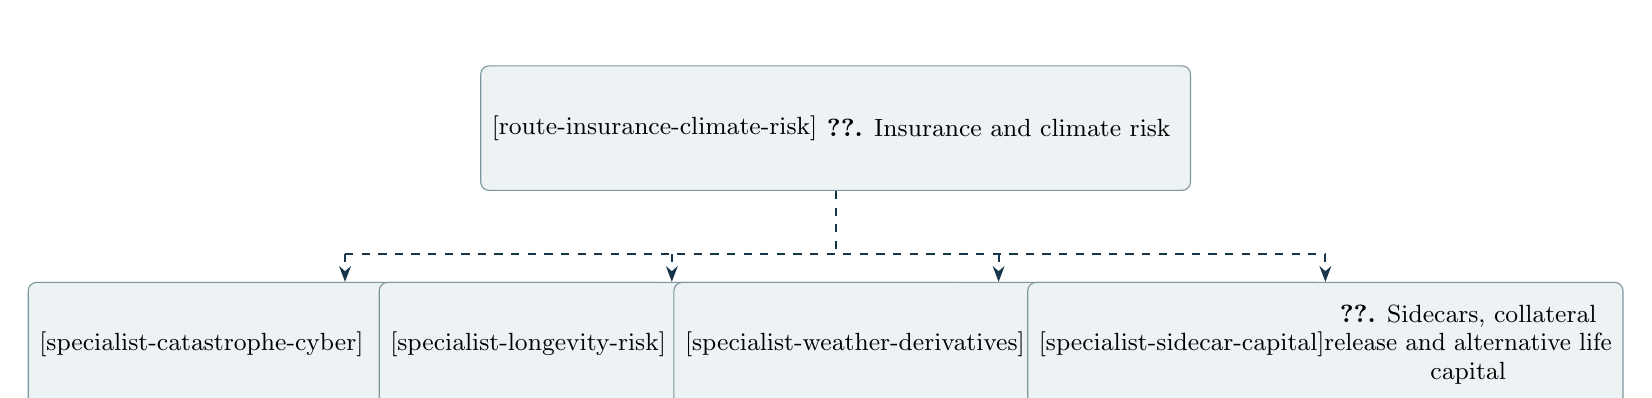
\begin{tikzpicture}[x=1cm,y=1cm]
\node[pathnode] (insurance-climate-risk) at (6.23,0) {\MeasurePathNode{4.6cm}{\textbf{\ref*{route-insurance-climate-risk}.} Insurance and climate risk}\hyperref[route-insurance-climate-risk]{\parbox[c][\pathnodeheight][c]{4.6cm}{\centering \textbf{\ref*{route-insurance-climate-risk}.} Insurance and climate risk}}};
\node[pathnode] (catastrophe-cyber) at (0.00,-2.75) {\MeasurePathNode{3.65cm}{\textbf{\ref*{specialist-catastrophe-cyber}.} Catastrophe and cyber insurance-linked risk}\hyperref[specialist-catastrophe-cyber]{\parbox[c][\pathnodeheight][c]{3.65cm}{\centering \textbf{\ref*{specialist-catastrophe-cyber}.} Catastrophe and cyber insurance-linked risk}}};
\node[pathnode] (longevity-risk) at (4.15,-2.75) {\MeasurePathNode{3.65cm}{\textbf{\ref*{specialist-longevity-risk}.} Mortality and longevity claims}\hyperref[specialist-longevity-risk]{\parbox[c][\pathnodeheight][c]{3.65cm}{\centering \textbf{\ref*{specialist-longevity-risk}.} Mortality and longevity claims}}};
\node[pathnode] (weather-derivatives) at (8.30,-2.75) {\MeasurePathNode{3.65cm}{\textbf{\ref*{specialist-weather-derivatives}.} Weather exposure and temperature derivatives}\hyperref[specialist-weather-derivatives]{\parbox[c][\pathnodeheight][c]{3.65cm}{\centering \textbf{\ref*{specialist-weather-derivatives}.} Weather exposure and temperature derivatives}}};
\node[pathnode] (sidecar-capital) at (12.45,-2.75) {\MeasurePathNode{3.65cm}{\textbf{\ref*{specialist-sidecar-capital}.} Sidecars, collateral release and alternative life capital}\hyperref[specialist-sidecar-capital]{\parbox[c][\pathnodeheight][c]{3.65cm}{\centering \textbf{\ref*{specialist-sidecar-capital}.} Sidecars, collateral release and alternative life capital}}};
\draw[entryline] (insurance-climate-risk.south) -- (6.23,-1.60);
\draw[entryline] (0.00,-1.60) -- (12.45,-1.60);
\draw[entryarrow] (0.00,-1.60) -- (catastrophe-cyber.north);
\draw[entryarrow] (4.15,-1.60) -- (longevity-risk.north);
\draw[entryarrow] (8.30,-1.60) -- (weather-derivatives.north);
\draw[entryarrow] (12.45,-1.60) -- (sidecar-capital.north);
\end{tikzpicture}\end{center}
\hyperref[learning-map]{Return to the whole-guide DAG.}
\Needspace{12\baselineskip}
\subsection{Catastrophe and cyber insurance-linked risk}\label{specialist-catastrophe-cyber}
\textbf{Specialist pathway.} In \hyperref[route-insurance-climate-risk]{Insurance and climate-linked risk}.

\textbf{Outcome.} Assess natural-catastrophe and cyber bond cash flows from triggers, loss distributions and collateral.

\textbf{Prerequisites.} Insurance and climate-linked risk; probability tails, reinsurance attachment and collateral cash flows.

\textbf{Review first.} \hyperref[route-insurance-climate-risk]{Insurance and climate-linked risk}.

\textbf{Required readings, in order}
\begin{enumerate}\raggedright
\Needspace{5\baselineskip}\item \href{institutional_quantitative_finance_reading_list.pdf\#ils-froot-cat-market-2001}{Kenneth A. Froot, The Market for Catastrophe Risk: A Clinical Examination}\CataloguePage{430}\NoteKey{ils-froot-cat-market-2001}\par \textbf{Mechanics.} Understand the economic role of catastrophe risk transfer.
\Needspace{5\baselineskip}\item \href{institutional_quantitative_finance_reading_list.pdf\#ils-braun-primary-pricing-2016}{Alexander Braun, Pricing in the Primary Market for Cat Bonds: New Empirical Evidence}\CataloguePage{430}\NoteKey{ils-braun-primary-pricing-2016}\par \textbf{Evidence.} Compare primary issue spreads with risk and market conditions.
\Needspace{5\baselineskip}\item \href{institutional_quantitative_finance_reading_list.pdf\#depth-naic-oep-aep}{National Association of Insurance Commissioners, Catastrophe Models (Property); Catastrophe Model Primer, ``Key Metrics and Outputs''}\CataloguePage{433}\NoteKey{depth-naic-oep-aep}\par \textbf{Valuation.} Interpret occurrence and aggregate exceedance curves.
\Needspace{5\baselineskip}\item \href{institutional_quantitative_finance_reading_list.pdf\#depth-liu-robust-cat}{Haibo Liu, Robust Indifference Valuation of Catastrophe Bonds}\CataloguePage{433}\NoteKey{depth-liu-robust-cat}\par \textbf{Valuation.} Stress distribution and model uncertainty in catastrophe loss.
\Needspace{5\baselineskip}\item \href{institutional_quantitative_finance_reading_list.pdf\#ils-teh-woolnough-trigger-2019}{Tse-Ling Teh and Christopher Woolnough, A Better Trigger: Indices for Insurance}\CataloguePage{430}\NoteKey{ils-teh-woolnough-trigger-2019}\par \textbf{Mechanics.} Distinguish indemnity, index and parametric trigger basis.
\Needspace{5\baselineskip}\item \href{institutional_quantitative_finance_reading_list.pdf\#ils-worldbank-mexico-catbond-2025}{World Bank, World Bank Catastrophe Bonds Provide Mexico with \$595 Million Financial Protection against Hurricanes and Earthquakes}\CataloguePage{431}\NoteKey{ils-worldbank-mexico-catbond-2025}\par \textbf{Data.} Trace a public transaction's payout and reporting terms.
\Needspace{5\baselineskip}\item \href{institutional_quantitative_finance_reading_list.pdf\#ils-swissre-market-july-2026}{Swiss Re Alternative Capital Partners, ILS Market Insights: July 2026}\CataloguePage{431}\NoteKey{ils-swissre-market-july-2026}\par \textbf{Evidence.} Check current issuance and pricing context with dated scope.
\Needspace{5\baselineskip}\item \href{institutional_quantitative_finance_reading_list.pdf\#add-cyber-model}{O. Kolesnikov, A. Markov, D. Smagulov and S. Solovjovs, Cyber Loss Distribution Fitting: A General Framework towards Cyber Bonds and Their Pricing Models}\CataloguePage{431}\NoteKey{add-cyber-model}\par \textbf{Valuation.} Model cyber loss frequency, severity and correlated events.
\Needspace{5\baselineskip}\item \href{institutional_quantitative_finance_reading_list.pdf\#add-cyber-issue}{Conyers, PoleStar Re Ltd. US\$300 Million Series 2026-1 Note Offering and Listing}\CataloguePage{431}\NoteKey{add-cyber-issue}\par \textbf{Mechanics.} Confirm the completed cyber issue and identify missing offering terms.
\Needspace{5\baselineskip}\item \href{institutional_quantitative_finance_reading_list.pdf\#evidence-slide-collateral}{Slide Insurance / White Rock Insurance (SAC), account T104, Aggregate Catastrophe Excess of Loss Reinsurance Contract}\CataloguePage{434}\NoteKey{evidence-slide-collateral}\par \textbf{Implementation.} Compare collateral release in a reinsurance contract; do not transfer its formula to a cat bond.
\Needspace{5\baselineskip}\item \href{institutional_quantitative_finance_reading_list.pdf\#w3-tomunen-disaster-risk}{Tuomas Tomunen, ``Failure to Share Natural Disaster Risk''}\CataloguePage{433}\NoteKey{w3-tomunen-disaster-risk}\par \textbf{Evidence.} Explain cat-bond expected returns with intermediary exposure.
\end{enumerate}
\Needspace{5\baselineskip}\textbf{Checkpoint.} Construct separate occurrence, aggregate and hypothetical cyber loss scenarios. Use the public Mexico bond documents to map its trigger to principal loss and collateral return; do not import release terms from the separate reinsurance agreement. Treat loss and spread estimates as model-dependent. Keep cyber scenarios hypothetical until offering terms are available. Identify missing exposure, catastrophe-model and incident data.

\textbf{Optional branches.} \href{institutional_quantitative_finance_reading_list.pdf\#wide-wang-transform}{Price cat risk with distortion operators.}\BranchPage{432} \href{institutional_quantitative_finance_reading_list.pdf\#wide-mitchell-wallace-catmodel}{Read a practitioner catastrophe-modelling guide.}\BranchPage{432}
\par{\small \hyperref[learning-map]{Learning pathway DAG} \textbar{} \hyperref[route-insurance-climate-risk]{Section overview} \textbar{} \hyperref[map-insurance-climate-risk]{Section DAG}\NoteKey{catastrophe-cyber}}
\Needspace{12\baselineskip}
\subsection{Mortality and longevity claims}\label{specialist-longevity-risk}
\textbf{Specialist pathway.} In \hyperref[route-insurance-climate-risk]{Insurance and climate-linked risk}.

\textbf{Outcome.} Price longevity exposure while separating population, basis, collateral and regulatory capital effects.

\textbf{Prerequisites.} Insurance and climate-linked risk; survival probabilities and annuity cash flows.

\textbf{Review first.} \hyperref[route-insurance-climate-risk]{Insurance and climate-linked risk}.

\textbf{Required readings, in order}
\begin{enumerate}\raggedright
\Needspace{5\baselineskip}\item \href{institutional_quantitative_finance_reading_list.pdf\#gapclose-ons-life-tables}{Office for National Statistics, National life tables: UK; 2022--2024 release}\CataloguePage{432}\NoteKey{gapclose-ons-life-tables}\par \textbf{Data.} Start with a public UK period table, preserving the release vintage before introducing mortality improvement and population basis risk.
\Needspace{5\baselineskip}\item \href{institutional_quantitative_finance_reading_list.pdf\#add-mortality-data}{Human Mortality Database, Overview, country data and methods}\CataloguePage{431}\NoteKey{add-mortality-data}\par \textbf{Data.} Select country, cohort and table vintages and inspect age, coverage and registration limits.
\Needspace{5\baselineskip}\item \href{institutional_quantitative_finance_reading_list.pdf\#ils-cairns-blake-dowd-mortality-2006}{Andrew J. G. Cairns, David Blake, and Kevin Dowd, A Two-Factor Model for Stochastic Mortality with Parameter Uncertainty: Theory and Calibration; Author-hosted manuscript}\CataloguePage{431}\NoteKey{ils-cairns-blake-dowd-mortality-2006}\par \textbf{Valuation.} Build a stochastic mortality and survival forecast.
\Needspace{5\baselineskip}\item \href{institutional_quantitative_finance_reading_list.pdf\#ils-blake-longevity-bonds-2006}{David Blake, Andrew Cairns, Kevin Dowd, and Richard MacMinn, Longevity Bonds: Financial Engineering, Valuation, and Hedging}\CataloguePage{432}\NoteKey{ils-blake-longevity-bonds-2006}\par \textbf{Mechanics.} Understand security cash flows linked to cohort survival.
\Needspace{5\baselineskip}\item \href{institutional_quantitative_finance_reading_list.pdf\#ils-coughlan-longevity-basis-2011}{Guy D. Coughlan, Marwa Khalaf-Allah, Yijing Ye, Sumit Kumar, Andrew J. G. Cairns, David Blake, and Kevin Dowd, Longevity Hedging 101: A Framework for Longevity Basis Risk Analysis and Hedge Effectiveness; Author-hosted working manuscript}\CataloguePage{432}\NoteKey{ils-coughlan-longevity-basis-2011}\par \textbf{Evidence.} Measure hedge basis between an index and a pension population.
\Needspace{5\baselineskip}\item \href{institutional_quantitative_finance_reading_list.pdf\#depth-kallestrup-longevity-basis}{Malene Kallestrup-Lamb and Nicolai Søgaard Laursen, Longevity Hedge Effectiveness Using Socioeconomic Indices; author-university open copy}\CataloguePage{434}\NoteKey{depth-kallestrup-longevity-basis}\par \textbf{Valuation.} Refine index-to-book population basis risk.
\Needspace{5\baselineskip}\item \href{institutional_quantitative_finance_reading_list.pdf\#depth-landriault-longevity-swaps}{David Landriault, Bin Li, Hong Li and Yuanyuan Zhang, Contract Structure and Risk Aversion in Longevity Risk Transfers; university open copy}\CataloguePage{434}\NoteKey{depth-landriault-longevity-swaps}\par \textbf{Mechanics.} Trace swap cash flows and counterparty terms.
\Needspace{5\baselineskip}\item \href{institutional_quantitative_finance_reading_list.pdf\#depth-pra-longevity-capital}{UK Prudential Regulation Authority, SS18/16: Longevity Risk Transfers; DP2/25: Alternative Life Capital}\CataloguePage{435}\NoteKey{depth-pra-longevity-capital}\par \textbf{Implementation.} Link hedge benefit to capital rules and governance.
\end{enumerate}
\Needspace{5\baselineskip}\textbf{Checkpoint.} Download the ONS UK table and record its observation window and release vintage. Reconstruct a period survival curve, then price an explicitly assumed cohort survival swap by adding mortality-improvement assumptions. Compare permitted HMD country data where available. Show payer/receiver cash flows, collateral, population basis and capital effects; separate national-table evidence from insured experience and live hedge quotes.

\textbf{Optional branches.} \href{institutional_quantitative_finance_reading_list.pdf\#wide-lee-carter}{Fit the Lee--Carter benchmark mortality model.}\BranchPage{432}
\par{\small \hyperref[learning-map]{Learning pathway DAG} \textbar{} \hyperref[route-insurance-climate-risk]{Section overview} \textbar{} \hyperref[map-insurance-climate-risk]{Section DAG}\NoteKey{longevity-risk}}
\Needspace{12\baselineskip}
\subsection{Weather exposure and temperature derivatives}\label{specialist-weather-derivatives}
\textbf{Specialist pathway.} In \hyperref[route-insurance-climate-risk]{Insurance and climate-linked risk}.

\textbf{Outcome.} Build a station-level weather exposure model, map it to a listed HDD/CDD payoff, and quantify station, observation and settlement basis.

\textbf{Prerequisites.} Insurance and climate-linked risk; elementary weather time series, options and contract multipliers.

\textbf{Review first.} \hyperref[route-insurance-climate-risk]{Insurance and climate-linked risk}.

\textbf{Required readings, in order}
\begin{enumerate}\raggedright
\Needspace{5\baselineskip}\item \href{institutional_quantitative_finance_reading_list.pdf\#weather-jewson-brix-2005}{Stephen Jewson and Anders Brix, with contributions by Christine Ziehmann, Weather Derivative Valuation: The Meteorological, Statistical, Financial and Mathematical Foundations; Publisher chapter contents and online-date distinction}\CataloguePage{386}\NoteKey{weather-jewson-brix-2005}\par\emph{Selection:} Weather-index and risk-modeling chapters.\par \textbf{Valuation.} Model degree-day distributions, seasonality and hedge design.
\Needspace{5\baselineskip}\item \href{institutional_quantitative_finance_reading_list.pdf\#weather-noaa-normals-1991-2020}{NOAA National Centers for Environmental Information, 1991--2020 U.S. Climate Normals}\CataloguePage{386}\NoteKey{weather-noaa-normals-1991-2020}\par \textbf{Data.} Define climatological baseline and station normals without treating normals as daily settlement observations.
\Needspace{5\baselineskip}\item \href{institutional_quantitative_finance_reading_list.pdf\#breadth-noaa-ghcnd-daily}{NOAA National Centers for Environmental Information, Global Historical Climatology Network--Daily (GHCNd)}\CataloguePage{387}\NoteKey{breadth-noaa-ghcnd-daily}\par \textbf{Data.} Assemble a quality-flagged daily temperature proxy with vintage and missingness controls.
\Needspace{5\baselineskip}\item \href{institutional_quantitative_finance_reading_list.pdf\#weather-benth-benth-2007}{Fred Espen Benth and Jūratė Šaltytė Benth, The Volatility of Temperature and Pricing of Weather Derivatives; Publisher article abstract and DOI}\CataloguePage{386}\NoteKey{weather-benth-benth-2007}\par \textbf{Evidence.} Evaluate a historical temperature model, respecting its station and sample limits.
\Needspace{5\baselineskip}\item \href{institutional_quantitative_finance_reading_list.pdf\#weather-cme-contracts}{CME Group, Weather Options Overview and Weather Futures and Options; CME HDD/CDD fact card}\CataloguePage{386}\NoteKey{weather-cme-contracts}\par \textbf{Mechanics.} Introduce CME HDD/CDD listed exposure and monthly cash settlement.
\Needspace{5\baselineskip}\item \href{institutional_quantitative_finance_reading_list.pdf\#breadth-cme-weather-rule403}{CME Group, CME Rulebook Chapter 403: Monthly Temperature Futures}\CataloguePage{386}\NoteKey{breadth-cme-weather-rule403}\par \textbf{Implementation.} Implement the named station, NWS/Speedwell source, local-standard-time day, degree-day formula and final settlement calendar.
\Needspace{5\baselineskip}\item \href{institutional_quantitative_finance_reading_list.pdf\#ils-teh-woolnough-trigger-2019}{Tse-Ling Teh and Christopher Woolnough, A Better Trigger: Indices for Insurance}\CataloguePage{430}\NoteKey{ils-teh-woolnough-trigger-2019}\par \textbf{Evidence.} Frame index-trigger basis risk rather than claiming a weather hedge perfectly offsets operating loss.
\Needspace{5\baselineskip}\item \href{institutional_quantitative_finance_reading_list.pdf\#w6-campbell-diebold-weather}{Sean D. Campbell and Francis X. Diebold, ``Weather Forecasting for Weather Derivatives''}\CataloguePage{387}\NoteKey{w6-campbell-diebold-weather}\par \textbf{Methods.} Model daily temperature for degree-day pricing.
\end{enumerate}
\Needspace{5\baselineskip}\textbf{Checkpoint.} For a named CME city/month, compute a proxy daily HDD/CDD series from a dated NOAA station extract and a weather-sensitive revenue series. Price and stress a \$20-per-index-point contract under the current Rule 403 formula; separately obtain or flag missing official Speedwell final index, station mismatch, missing days, local-standard-time treatment and market liquidity before reporting hedge effectiveness.

\textbf{Optional branches.} \href{institutional_quantitative_finance_reading_list.pdf\#ils-cummins-weiss-convergence-2009}{Compare listed temperature hedges with catastrophe trigger design.}\BranchPage{430} \href{institutional_quantitative_finance_reading_list.pdf\#weather-noaa-normals-1991-2020}{Repeat with another climate-normal baseline to test nonstationarity.}\BranchPage{386} \href{institutional_quantitative_finance_reading_list.pdf\#w6-alaton-weather}{Price degree-day options with a mean-reverting temperature model.}\BranchPage{387} \href{institutional_quantitative_finance_reading_list.pdf\#w6-perez-gonzalez-yun}{Link weather hedging to firm value.}\BranchPage{387} \href{institutional_quantitative_finance_reading_list.pdf\#w6-purnanandam-weagley}{Check weather-station data integrity behind index contracts.}\BranchPage{387}
\par{\small \hyperref[learning-map]{Learning pathway DAG} \textbar{} \hyperref[route-insurance-climate-risk]{Section overview} \textbar{} \hyperref[map-insurance-climate-risk]{Section DAG}\NoteKey{weather-derivatives}}
\Needspace{12\baselineskip}
\subsection{Sidecars, collateral release and alternative life capital}\label{specialist-sidecar-capital}
\textbf{Specialist pathway.} In \hyperref[route-insurance-climate-risk]{Insurance and climate-linked risk}.

\textbf{Outcome.} Separate insurance capacity, capital commitments, paid-in funds, collateral release and investor distributions.

\textbf{Prerequisites.} Insurance and climate-linked risk; insurance balance sheets, claims development and private-fund cash flows.

\textbf{Review first.} \hyperref[route-insurance-climate-risk]{Insurance and climate-linked risk}.

\textbf{Required readings, in order}
\begin{enumerate}\raggedright
\Needspace{5\baselineskip}\item \href{institutional_quantitative_finance_reading_list.pdf\#ils-cummins-weiss-convergence-2009}{J. David Cummins and Mary A. Weiss, Convergence of Insurance and Financial Markets: Hybrid and Securitized Risk-Transfer Solutions}\CataloguePage{430}\NoteKey{ils-cummins-weiss-convergence-2009}\par \textbf{Architecture.} Understand insurance-risk securitisation before comparing a cat bond with a proportional sidecar.
\Needspace{5\baselineskip}\item \href{institutional_quantitative_finance_reading_list.pdf\#depth-aon-sidecar-2026}{Aon Reinsurance Solutions, Reinsurance Market Dynamics, April 2026}\CataloguePage{434}\NoteKey{depth-aon-sidecar-2026}\par \textbf{Market evidence.} Interpret capacity growth as a broker estimate, with casualty and multiline structure differences.
\Needspace{5\baselineskip}\item \href{institutional_quantitative_finance_reading_list.pdf\#evidence-slide-collateral}{Slide Insurance / White Rock Insurance (SAC), account T104, Aggregate Catastrophe Excess of Loss Reinsurance Contract}\CataloguePage{434}\NoteKey{evidence-slide-collateral}\par \textbf{Contract mechanics.} Trace the selected reinsurance release, commutation and limited-recourse provisions; this is not the investor LPA.
\Needspace{5\baselineskip}\item \href{institutional_quantitative_finance_reading_list.pdf\#evidence-upsilon-capital}{RenaissanceRe, 2025 Form 10-K, variable-interest-entity note: Upsilon RFO}\CataloguePage{434}\NoteKey{evidence-upsilon-capital}\par \textbf{Observed runoff.} Distinguish cedant collateral release from subsequent investor capital returned and profit.
\Needspace{5\baselineskip}\item \href{institutional_quantitative_finance_reading_list.pdf\#gapclose-sidecar-commitment}{AllianceBernstein L.P., June 2026 Form 10-Q, commitments note on RGA and FCA Re sidecars}\CataloguePage{434}\NoteKey{gapclose-sidecar-commitment}\par \textbf{Investor disclosure.} Reconcile commitments with funded amounts for the dated life/annuity sidecar cases.
\Needspace{5\baselineskip}\item \href{institutional_quantitative_finance_reading_list.pdf\#depth-pra-longevity-capital}{UK Prudential Regulation Authority, SS18/16: Longevity Risk Transfers; DP2/25: Alternative Life Capital}\CataloguePage{435}\NoteKey{depth-pra-longevity-capital}\par \textbf{Life capital and counterparty risk.} Study longevity transfer and alternative life capital on their own regulatory and liability basis.
\end{enumerate}
\Needspace{5\baselineskip}\textbf{Checkpoint.} Create dated ledgers for committed, called, invested and collateralised capital, developed claims, released collateral and investor distributions. Use the issuer disclosures only for the quantities actually reported. Compare catastrophe/casualty runoff with asset-intensive life liabilities. Supply an explicit scenario for missing calls, fees and losses; an actual net IRR requires the executed investor agreement and complete dated contributions/distributions.

\textbf{Optional branches.} \href{institutional_quantitative_finance_reading_list.pdf\#w6-lakdawalla-zanjani}{Explain collateralised reinsurance and cat bonds.}\BranchPage{435} \href{institutional_quantitative_finance_reading_list.pdf\#w6-gurtler-catbonds}{See cat-bond spreads in crises.}\BranchPage{435} \href{institutional_quantitative_finance_reading_list.pdf\#w6-ge-insurance-pricing}{Trace insurer capital shocks into pricing.}\BranchPage{435}
\par{\small \hyperref[learning-map]{Learning pathway DAG} \textbar{} \hyperref[route-insurance-climate-risk]{Section overview} \textbar{} \hyperref[map-insurance-climate-risk]{Section DAG}\NoteKey{sidecar-capital}}
\clearpage
\part{Digital assets}\label{part-digital-assets}
Apply earlier pricing, market-making and validation tools to digital-asset venues and derivatives, crypto spot markets, on-chain claims, fractional and tokenised assets, market making on centralised and decentralised venues, and crypto trading strategies. Event contracts, including on-chain prediction markets, are in Part VII.

\textbf{Sections in learning order}\begin{enumerate}
\item[\ref*{route-digital-assets-prediction-markets}.] \hyperref[route-digital-assets-prediction-markets]{Crypto settlement, venues and derivatives} --- Begin with custody, settlement and stablecoin collateral, then progress through cross-venue basis and crypto options. Three later pathways deepen each strand: stablecoin pegs and runs, leverage and liquidation cascades, and option-market evidence. Spot price discovery, exchange market quality, valuation, investors and exchange regulation follow in Section 31; order-book dealing and other market making are in Section 34.
\item[\ref*{route-crypto-spot-markets}.] \hyperref[route-crypto-spot-markets]{Crypto spot markets: price discovery, market quality, valuation and investors} --- Price discovery, exchange market quality and valuation are separate entry points. Investors and spot ETFs build on price discovery; exchange failures and regulation build on market quality; return dynamics build on valuation. Derivatives on the same assets are in Section 30; on-chain trading and crypto return signals follow in Section 32.
\item[\ref*{route-onchain-protocols}.] \hyperref[route-onchain-protocols]{On-chain protocols} --- Automated market makers, transaction ordering, staking, protocol risk and on-chain signals are separate entry points. Lending, liquidations and oracles build on AMMs; solver execution builds on both AMMs and transaction ordering. Tokenised securities traded in permissioned AMM pools are covered in Section 33.
\item[\ref*{route-tokenised-fractional-assets}.] \hyperref[route-tokenised-fractional-assets]{Fractional and tokenised assets: fractional shares, tokenised securities and real-world assets} --- Fractional shares and tokenised securities are separate entry points. Token offerings and tokenised real assets build on tokenised securities. Stablecoins, tokenised bonds and tokenised money market funds are in 30.1.
\item[\ref*{route-crypto-market-making}.] \hyperref[route-crypto-market-making]{Crypto market making: order books, DEX liquidity and token market makers} --- Order-book dealing and RFQ, order-book microstructure, token market makers and DEX liquidity provision are separate entry points; quoting strategies and learning agents build on order-book microstructure. AMM pricing and LP returns are in Section 32; exchange market quality and wash trading are in Section 31; perpetual hedging is in Section 30.
\item[\ref*{route-crypto-trading-strategies}.] \hyperref[route-crypto-trading-strategies]{Crypto trading strategies: factors, trend, arbitrage, sentiment and machine learning} --- Cross-sectional factors, trend and technical rules, statistical arbitrage, arbitrage and carry, and sentiment and event strategies are separate entry points; machine-learning prediction builds on the cross-sectional pathway. Market making is in Section 34; on-chain signals and wallet data are in Crypto signals and on-chain evidence (32.7); option and volatility strategies are in Section 30.
\end{enumerate}
\hyperref[learning-map]{Return to the learning pathway DAG.}
\clearpage
\section{Crypto settlement, venues and derivatives}\label{route-digital-assets-prediction-markets}
\label{route-10}
\textbf{Learning sequence.} Begin with custody, settlement and stablecoin collateral, then progress through cross-venue basis and crypto options. Three later pathways deepen each strand: stablecoin pegs and runs, leverage and liquidation cascades, and option-market evidence. Spot price discovery, exchange market quality, valuation, investors and exchange regulation follow in Section 31; order-book dealing and other market making are in Section 34.

\textbf{Section goals.} Across its pathways, this section teaches you to:
\begin{itemize}[leftmargin=1.4em,itemsep=0pt,topsep=1pt]
\item trace stablecoin and tokenised-bond claims, reserves and redemption (\hyperref[specialist-stablecoin-tokenisation]{\ref*{specialist-stablecoin-tokenisation}})
\item reconcile spot, perpetual and dated-futures basis across venues (\hyperref[specialist-crypto-perpetuals]{\ref*{specialist-crypto-perpetuals}})
\item explain stablecoin pegs and stress the channels of a run (\hyperref[specialist-stablecoin-pegs-runs]{\ref*{specialist-stablecoin-pegs-runs}})
\item price and hedge linear and inverse crypto options in their settlement units (\hyperref[specialist-crypto-options-numeraire]{\ref*{specialist-crypto-options-numeraire}})
\item map crypto leverage and model liquidation cascades (\hyperref[specialist-crypto-leverage-liquidations]{\ref*{specialist-crypto-leverage-liquidations}})
\item build bitcoin volatility surfaces and decompose option premia (\hyperref[specialist-crypto-option-markets]{\ref*{specialist-crypto-option-markets}})
\end{itemize}
\textbf{Overview outcome.} Trace a crypto position from custody and collateral through venue fragmentation, funding, quoting and option margin to its settlement risk.

\textbf{Prerequisites.} Common toolkit; basic exchange microstructure, wallet transactions and futures or option payoffs.

\textbf{Review first.} \hyperref[route-common-toolkit]{Common toolkit}.

\textbf{Required readings, in order}
\begin{enumerate}\raggedright
\Needspace{5\baselineskip}\item \href{institutional_quantitative_finance_reading_list.pdf\#crypto-narayanan}{Arvind Narayanan, Joseph Bonneau, Edward Felten, Andrew Miller and Steven Goldfeder, \emph{Bitcoin and Cryptocurrency Technologies} (Princeton University Press, 2016)}\CataloguePage{436}\NoteKey{crypto-narayanan}\par Establish consensus, transactions and custody before analysing a token-market strategy.
\Needspace{5\baselineskip}\item \href{institutional_quantitative_finance_reading_list.pdf\#wide-john-ohara-saleh}{Kose John, Maureen O'Hara and Fahad Saleh, ``Bitcoin and Beyond''}\CataloguePage{437}\NoteKey{wide-john-ohara-saleh}\par Survey consensus, mining, stablecoins, DeFi and regulation as economic mechanisms before choosing a venue or protocol pathway.
\Needspace{5\baselineskip}\item \href{institutional_quantitative_finance_reading_list.pdf\#s6-makarov}{Igor Makarov and Antoinette Schoar, ``Trading and Arbitrage in Cryptocurrency Markets''; LSE discussion paper}\CataloguePage{438}\NoteKey{s6-makarov}\par Examine cross-venue crypto arbitrage with the transfer and settlement frictions that constrain it.
\end{enumerate}
\Needspace{5\baselineskip}\textbf{Checkpoint, a section capstone: complete it after \hyperref[specialist-stablecoin-tokenisation]{\ref*{specialist-stablecoin-tokenisation}}, \hyperref[specialist-crypto-perpetuals]{\ref*{specialist-crypto-perpetuals}} and \hyperref[specialist-crypto-options-numeraire]{\ref*{specialist-crypto-options-numeraire}}.} For one perpetual future and one dated option on the same token, draw the path from deposited collateral to liquidation or settlement. Record the index, funding, margin and settlement-currency rules; compute the cross-venue basis net of transfer, funding and withdrawal frictions, then identify which leg fails first if a stablecoin used as collateral trades below par.

\textbf{Optional branches.} \href{institutional_quantitative_finance_reading_list.pdf\#section.18.8}{Add stablecoin reserves, redemption and tokenised-claim settlement.}\BranchPage{485} \href{institutional_quantitative_finance_reading_list.pdf\#crypto-unic-blockchain-digital-assets}{Use the current published syllabus as an introductory roadmap; the next advertised cohort begins in February 2027.}\BranchPage{545} \href{institutional_quantitative_finance_reading_list.pdf\#roadmap-mastering-bitcoin}{Use the transaction-programming selections to trace UTXOs, fees and settlement before exchange-transfer research.}\BranchPage{436} \href{institutional_quantitative_finance_reading_list.pdf\#wide-budish-bitcoin-limits}{Study the economic limits of Nakamoto consensus.}\BranchPage{437} \href{institutional_quantitative_finance_reading_list.pdf\#s6-bitcoin}{Read the original white paper for the settlement and issuance assumptions that later venue and custody rules rely on.}\BranchPage{437} \href{institutional_quantitative_finance_reading_list.pdf\#w2-stanford-cs251}{Use the public lecture slides for a rigorous course on consensus, Ethereum, DeFi and scaling.}\BranchPage{545}
\par\textbf{Continue in this section.} \hyperref[specialist-stablecoin-tokenisation]{Stablecoins and tokenised bonds}; \hyperref[specialist-crypto-perpetuals]{Crypto perpetuals and cross-venue basis}; \hyperref[specialist-stablecoin-pegs-runs]{Stablecoin pegs, runs and reserve assets}; \hyperref[specialist-crypto-options-numeraire]{Crypto options, inverse payoffs and margin}; \hyperref[specialist-crypto-leverage-liquidations]{Crypto leverage, liquidations and centralised lenders}; \hyperref[specialist-crypto-option-markets]{Crypto option markets: implied volatility, smiles and risk premia}.
\par{\small \hyperref[learning-map]{Learning pathway DAG} \textbar{} \hyperref[digital-map]{Section DAG}\NoteKey{digital-assets-prediction-markets}}
\clearpage
\subsection*{Crypto settlement, venues and derivatives: pathway DAG}\phantomsection\label{digital-map}
\addcontentsline{toc}{subsection}{Crypto settlement, venues and derivatives: pathway DAG}
Start with the section overview's readings, for orientation. Solid arrows show prerequisites within this section. Dashed connectors identify entry points with no further prerequisite in this section; the linked foundations below still apply. Follow the arrows for dependencies and the subsection numbers for reading order. Every node is clickable.
\begin{center}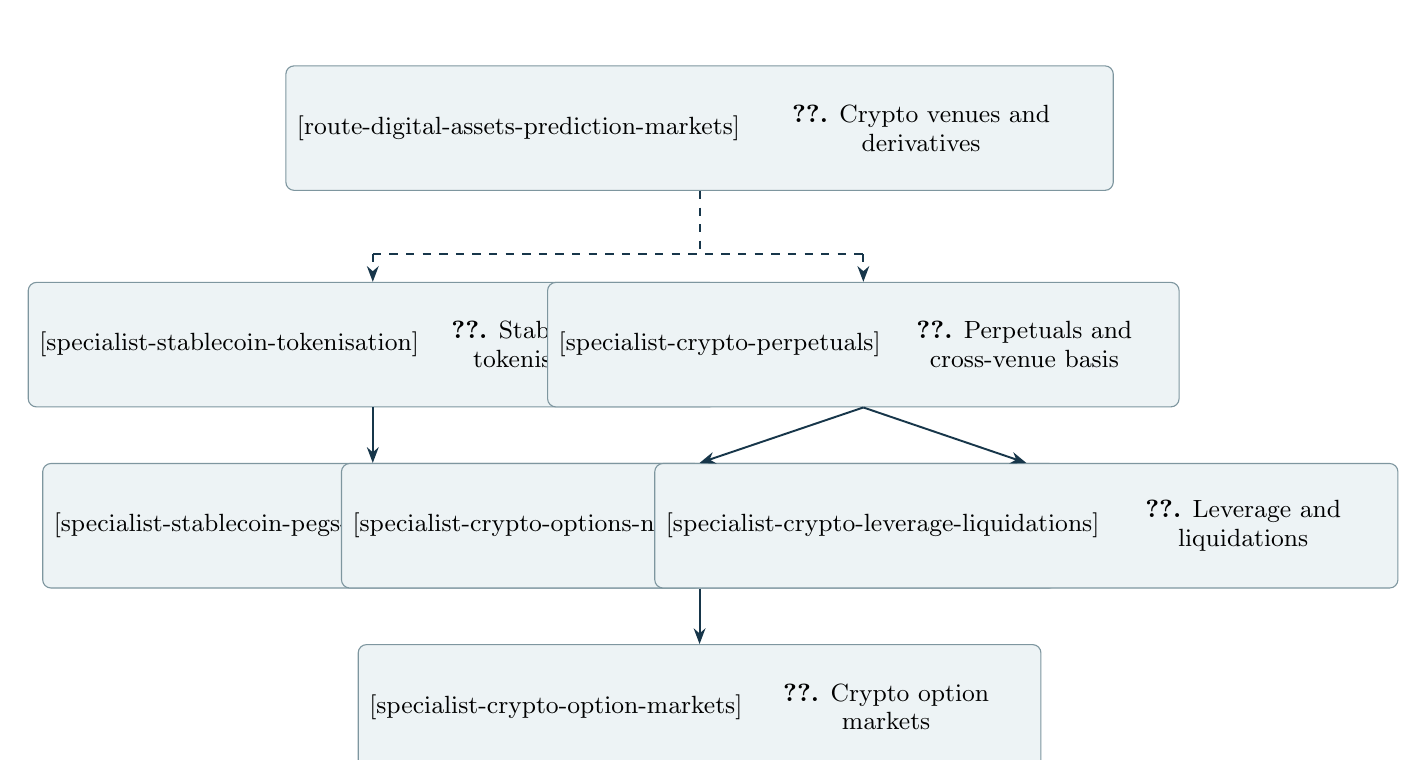
\begin{tikzpicture}[x=1cm,y=1cm]
\node[pathnode] (digital-assets-prediction-markets) at (4.15,0) {\MeasurePathNode{4.6cm}{\textbf{\ref*{route-digital-assets-prediction-markets}.} Crypto venues and derivatives}\hyperref[route-digital-assets-prediction-markets]{\parbox[c][\pathnodeheight][c]{4.6cm}{\centering \textbf{\ref*{route-digital-assets-prediction-markets}.} Crypto venues and derivatives}}};
\node[pathnode] (stablecoin-tokenisation) at (0.00,-2.75) {\MeasurePathNode{3.65cm}{\textbf{\ref*{specialist-stablecoin-tokenisation}.} Stablecoins and tokenised bonds}\hyperref[specialist-stablecoin-tokenisation]{\parbox[c][\pathnodeheight][c]{3.65cm}{\centering \textbf{\ref*{specialist-stablecoin-tokenisation}.} Stablecoins and tokenised bonds}}};
\node[pathnode] (crypto-perpetuals) at (6.23,-2.75) {\MeasurePathNode{3.65cm}{\textbf{\ref*{specialist-crypto-perpetuals}.} Perpetuals and cross-venue basis}\hyperref[specialist-crypto-perpetuals]{\parbox[c][\pathnodeheight][c]{3.65cm}{\centering \textbf{\ref*{specialist-crypto-perpetuals}.} Perpetuals and cross-venue basis}}};
\node[pathnode] (stablecoin-pegs-runs) at (0.00,-5.05) {\MeasurePathNode{3.65cm}{\textbf{\ref*{specialist-stablecoin-pegs-runs}.} Stablecoin pegs and runs}\hyperref[specialist-stablecoin-pegs-runs]{\parbox[c][\pathnodeheight][c]{3.65cm}{\centering \textbf{\ref*{specialist-stablecoin-pegs-runs}.} Stablecoin pegs and runs}}};
\node[pathnode] (crypto-options-numeraire) at (4.15,-5.05) {\MeasurePathNode{3.65cm}{\textbf{\ref*{specialist-crypto-options-numeraire}.} Crypto options and margin}\hyperref[specialist-crypto-options-numeraire]{\parbox[c][\pathnodeheight][c]{3.65cm}{\centering \textbf{\ref*{specialist-crypto-options-numeraire}.} Crypto options and margin}}};
\node[pathnode] (crypto-leverage-liquidations) at (8.30,-5.05) {\MeasurePathNode{3.65cm}{\textbf{\ref*{specialist-crypto-leverage-liquidations}.} Leverage and liquidations}\hyperref[specialist-crypto-leverage-liquidations]{\parbox[c][\pathnodeheight][c]{3.65cm}{\centering \textbf{\ref*{specialist-crypto-leverage-liquidations}.} Leverage and liquidations}}};
\node[pathnode] (crypto-option-markets) at (4.15,-7.35) {\MeasurePathNode{3.65cm}{\textbf{\ref*{specialist-crypto-option-markets}.} Crypto option markets}\hyperref[specialist-crypto-option-markets]{\parbox[c][\pathnodeheight][c]{3.65cm}{\centering \textbf{\ref*{specialist-crypto-option-markets}.} Crypto option markets}}};
\draw[entryline] (digital-assets-prediction-markets.south) -- (4.15,-1.60);
\draw[entryline] (0.00,-1.60) -- (6.23,-1.60);
\draw[entryarrow] (0.00,-1.60) -- (stablecoin-tokenisation.north);
\draw[entryarrow] (6.23,-1.60) -- (crypto-perpetuals.north);
\draw[patharrow] (stablecoin-tokenisation.south) -- (stablecoin-pegs-runs.north);
\draw[patharrow] (crypto-perpetuals.south) -- (crypto-options-numeraire.north);
\draw[patharrow] (crypto-perpetuals.south) -- (crypto-leverage-liquidations.north);
\draw[patharrow] (crypto-options-numeraire.south) -- (crypto-option-markets.north);
\end{tikzpicture}\end{center}
\textbf{Overview checkpoint.} A section capstone: complete it after \hyperref[specialist-stablecoin-tokenisation]{\ref*{specialist-stablecoin-tokenisation}}, \hyperref[specialist-crypto-perpetuals]{\ref*{specialist-crypto-perpetuals}} and \hyperref[specialist-crypto-options-numeraire]{\ref*{specialist-crypto-options-numeraire}}.

\textbf{Bring these foundations with you.}\begin{itemize}
\item \hyperref[route-volatility-options]{Option pricing, volatility models and hedging} --- needed by \hyperref[specialist-crypto-options-numeraire]{Crypto options and margin}.
\end{itemize}\hyperref[learning-map]{Return to the whole-guide DAG.}
\Needspace{12\baselineskip}
\subsection{Stablecoins and tokenised bonds}\label{specialist-stablecoin-tokenisation}
\textbf{Specialist pathway.} In \hyperref[route-digital-assets-prediction-markets]{Crypto settlement, venues and derivatives}.

\textbf{Outcome.} Trace the legal claim, reserve assets, redemption queue and settlement leg behind token prices.

\textbf{Prerequisites.} Crypto settlement, venues and derivatives; money markets, custody and payment settlement.

\textbf{Review first.} \hyperref[route-digital-assets-prediction-markets]{Crypto settlement, venues and derivatives}.

\textbf{Required readings, in order}
\begin{enumerate}\raggedright
\Needspace{5\baselineskip}\item \href{institutional_quantitative_finance_reading_list.pdf\#exp-bis-stablecoins}{Bank for International Settlements, Anchoring Trust in Money: Innovation Beyond Stablecoins}\CataloguePage{486}\NoteKey{exp-bis-stablecoins}\par \textbf{Evidence.} Frame stablecoins against monetary and payment-system criteria.
\Needspace{5\baselineskip}\item \href{institutional_quantitative_finance_reading_list.pdf\#add-usdc-terms}{Circle, USDC Terms; Circle Mint tokenization and redemption lifecycle; USDC reserve and issuance disclosures; Circle Mint native-chain support}\CataloguePage{486}\NoteKey{add-usdc-terms}\par \textbf{Mechanics.} Read issuer redemption, reserve and eligible-holder terms.
\Needspace{5\baselineskip}\item \href{institutional_quantitative_finance_reading_list.pdf\#add-stablecoin-runs}{Yiming Ma, Yao Zeng and Anthony Lee Zhang, Stablecoin Runs and the Centralization of Arbitrage; author manuscript}\CataloguePage{486}\NoteKey{add-stablecoin-runs}\par \textbf{Evidence.} Study concentration of arbitrage and redemption during stress.
\Needspace{5\baselineskip}\item \href{institutional_quantitative_finance_reading_list.pdf\#gap-money-cp-cd-primer}{Matteo Aquilina, Andreas Schrimpf and Karamfil Todorov, CP and CDs Markets: A Primer}\CataloguePage{234}\NoteKey{gap-money-cp-cd-primer}\par \textbf{Valuation.} Understand cash and short-dated reserve-asset risks.
\Needspace{5\baselineskip}\item \href{institutional_quantitative_finance_reading_list.pdf\#gap-money-nmfp-data}{U.S. Securities and Exchange Commission, Form N-MFP Data Sets; SEC series and class identification file}\CataloguePage{235}\NoteKey{gap-money-nmfp-data}\par \textbf{Data.} Use fund and money-market holdings data as a reserve-risk comparator.
\Needspace{5\baselineskip}\item \href{institutional_quantitative_finance_reading_list.pdf\#exp-token-bonds}{Iñaki Aldasoro, Giulio Cornelli, Jon Frost, Priscilla Koo Wilkens, Ulf Lewrick and Vatsala Shreeti, Tokenisation of Government Bonds: Assessment and Roadmap}\CataloguePage{485}\NoteKey{exp-token-bonds}\par \textbf{Mechanics.} Trace tokenised security title and delivery-versus-payment.
\Needspace{5\baselineskip}\item \href{institutional_quantitative_finance_reading_list.pdf\#exp-gleif}{Global Legal Entity Identifier Foundation (GLEIF), Golden Copy and Delta Files}\CataloguePage{517}\NoteKey{exp-gleif}\par \textbf{Data.} Resolve issuer and counterparty identities consistently.
\Needspace{5\baselineskip}\item \href{institutional_quantitative_finance_reading_list.pdf\#exp-pfmi}{CPSS and IOSCO Technical Committee, Principles for Financial Market Infrastructures}\CataloguePage{539}\NoteKey{exp-pfmi}\par \textbf{Implementation.} Test settlement finality, custody and operational dependencies.
\Needspace{5\baselineskip}\item \href{institutional_quantitative_finance_reading_list.pdf\#latest-born-tokenised-bonds-2026}{Alexandra Born, Johanne Evrard, Claudia Lambert, Wagner Eduardo Schuster and Anna Tskhakaya, Tokenised Bonds: Assessing Efficiency and Liquidity in a Nascent Market}\CataloguePage{486}\NoteKey{latest-born-tokenised-bonds-2026}\par \textbf{Empirical comparison.} Assess early tokenised corporate-bond evidence while distinguishing estimated spreads from executable quotes and causal effects.
\Needspace{5\baselineskip}\item \href{institutional_quantitative_finance_reading_list.pdf\#wide-genius-act}{United States Congress, ``Guiding and Establishing National Innovation for U.S. Stablecoins (GENIUS) Act, Public Law 119-27''}\CataloguePage{486}\NoteKey{wide-genius-act}\par \textbf{Regulation.} Map the US payment-stablecoin regime: reserves, redemption and supervision under the 2025 Act.
\Needspace{5\baselineskip}\item \href{institutional_quantitative_finance_reading_list.pdf\#wide-mica}{European Parliament and Council, ``Regulation (EU) 2023/1114 on markets in crypto-assets (MiCA)''}\CataloguePage{486}\NoteKey{wide-mica}\par \textbf{Regulation.} Compare the EU regime for e-money and asset-referenced tokens.
\Needspace{5\baselineskip}\item \href{institutional_quantitative_finance_reading_list.pdf\#wide-bis-tmmf}{Bank for International Settlements, ``The rise of tokenised money market funds (BIS Bulletin No 115)''}\CataloguePage{487}\NoteKey{wide-bis-tmmf}\par \textbf{Evidence.} See tokenised money-market funds used as collateral and their liquidity mismatch.
\Needspace{5\baselineskip}\item \href{institutional_quantitative_finance_reading_list.pdf\#w2-bis-aer2025-nextgen}{Bank for International Settlements, ``The next-generation monetary and financial system (Annual Economic Report 2025, Chapter III)''}\CataloguePage{487}\NoteKey{w2-bis-aer2025-nextgen}\par \textbf{Evidence.} Compare stablecoins with the tokenised unified-ledger proposal and its singleness, elasticity and integrity tests.
\end{enumerate}
\Needspace{5\baselineskip}\textbf{Checkpoint.} Draw a token-to-dollar redemption and a tokenised-bond delivery-versus-payment flow. At each step identify legal obligor, asset custodian, settlement finality, cut-off, fee and delay; stress a concentrated redemption wave and collateral-market shock with dated disclosures. Compare a tokenised-bond efficiency claim with the sample size, spread construction and selection limitations of the ECB study.

\textbf{Optional branches.} \href{institutional_quantitative_finance_reading_list.pdf\#wide-gorton-zhang-wildcat}{Compare stablecoins with historical private banknotes.}\BranchPage{486} \href{institutional_quantitative_finance_reading_list.pdf\#w3-auer-monnet-shin-ledgers}{Study ledger governance of money.}\BranchPage{487}
\par{\small \hyperref[learning-map]{Learning pathway DAG} \textbar{} \hyperref[route-digital-assets-prediction-markets]{Section overview} \textbar{} \hyperref[digital-map]{Section DAG}\NoteKey{stablecoin-tokenisation}}
\Needspace{12\baselineskip}
\subsection{Crypto perpetuals and cross-venue basis}\label{specialist-crypto-perpetuals}
\textbf{Specialist pathway.} In \hyperref[route-digital-assets-prediction-markets]{Crypto settlement, venues and derivatives}.

\textbf{Outcome.} Reconcile spot, perpetual and dated-futures basis with feasible financing, transfer, margin and liquidation paths across fragmented venues.

\textbf{Prerequisites.} Crypto settlement, venues and derivatives; futures basis, order books and collateral risk. Reference-rate construction in Crypto price discovery (31.1) explains the index prices that perpetuals and dated futures settle against.

\textbf{Review first.} \hyperref[route-digital-assets-prediction-markets]{Crypto settlement, venues and derivatives}.

\textbf{Required readings, in order}
\begin{enumerate}\raggedright
\Needspace{5\baselineskip}\item \href{institutional_quantitative_finance_reading_list.pdf\#crypto-narayanan}{Arvind Narayanan, Joseph Bonneau, Edward Felten, Andrew Miller and Steven Goldfeder, \emph{Bitcoin and Cryptocurrency Technologies} (Princeton University Press, 2016)}\CataloguePage{436}\NoteKey{crypto-narayanan}\par \textbf{Mechanics.} Establish transaction and settlement foundations.
\Needspace{5\baselineskip}\item \href{institutional_quantitative_finance_reading_list.pdf\#s6-makarov}{Igor Makarov and Antoinette Schoar, ``Trading and Arbitrage in Cryptocurrency Markets''; LSE discussion paper}\CataloguePage{438}\NoteKey{s6-makarov}\par \textbf{Evidence.} Study cross-venue price dislocations and arbitrage limits.
\Needspace{5\baselineskip}\item \href{institutional_quantitative_finance_reading_list.pdf\#roadmap-carry}{Maik Schmeling, Andreas Schrimpf, Karamfil Todorov, Crypto carry; Official revised PDF}\CataloguePage{446}\NoteKey{roadmap-carry}\par \textbf{Evidence.} Explain spot-dated-futures carry through leverage demand and constrained arbitrage capital; keep it distinct from uncertain future perpetual funding.
\Needspace{5\baselineskip}\item \href{institutional_quantitative_finance_reading_list.pdf\#s6-cryptofactors}{Yukun Liu, Aleh Tsyvinski and Xi Wu, ``Common Risk Factors in Cryptocurrency''; NBER working paper}\CataloguePage{442}\NoteKey{s6-cryptofactors}\par \textbf{Evidence.} Control broad crypto risk before attributing basis returns.
\Needspace{5\baselineskip}\item \href{institutional_quantitative_finance_reading_list.pdf\#roadmap-perpetual-pricing}{Damien Ackerer, Julien Hugonnier, Urban Jermann, Perpetual Futures Pricing; Author preprint}\CataloguePage{446}\NoteKey{roadmap-perpetual-pricing}\par \textbf{Valuation.} Derive linear, inverse and quanto perpetual cash flows before choosing a venue-specific funding model.
\Needspace{5\baselineskip}\item \href{institutional_quantitative_finance_reading_list.pdf\#roadmap-perpetual-fundamentals}{Songrun He, Asaf Manela, Omri Ross, Victor von Wachter, Fundamentals of Perpetual Futures}\CataloguePage{446}\NoteKey{roadmap-perpetual-fundamentals}\par \textbf{Valuation.} Read the corrected version and derive a trading-cost band rather than assuming convergence at a fixed expiry.
\Needspace{5\baselineskip}\item \href{institutional_quantitative_finance_reading_list.pdf\#roadmap-crypto-yield-curves}{Philippe Bergault, Sébastien Bieber, Olivier Guéant, Wenkai Zhang, Cryptocurrencies and Interest Rates: Inferring Yield Curves in a Bondless Market}\CataloguePage{446}\NoteKey{roadmap-crypto-yield-curves}\par \textbf{Financing.} Infer derivative-implied curves, then compare them with financing actually available to the account.
\Needspace{5\baselineskip}\item \href{institutional_quantitative_finance_reading_list.pdf\#s11-r15}{Will Gornall, Martin Rinaldi and Yizhou Xiao, ``Perpetual Futures and Basis Risk: Evidence from Cryptocurrency''; 19 May 2025 manuscript; earlier-title draft}\CataloguePage{445}\NoteKey{s11-r15}\par \textbf{Valuation.} Analyse funding payments, constrained arbitrage and basis risk.
\Needspace{5\baselineskip}\item \href{institutional_quantitative_finance_reading_list.pdf\#s11-r16}{Julia Ko\'nczal, ``Pricing options on the cryptocurrency futures contracts'' (17 June 2025, v1)}\CataloguePage{446}\NoteKey{s11-r16}\par \textbf{Valuation.} Connect crypto futures to option calibration and tail scenarios.
\Needspace{5\baselineskip}\item \href{institutional_quantitative_finance_reading_list.pdf\#s11-r29}{Binance spot REST / WebSocket; Deribit APIs; selected BitMEX technical post; Coinbase engineering blog; OKX V5 API; OKX checksum change; Bitfinex books; Bitfinex raw books; Bitfinex checksum}\CataloguePage{476}\NoteKey{s11-r29}\par \textbf{Mechanics.} Read venue-specific API and execution documentation.
\Needspace{5\baselineskip}\item \href{institutional_quantitative_finance_reading_list.pdf\#gapclose-deribit-rules}{Deribit FZE, \emph{Exchange Rulebook} and Funding Specifications; Inverse Options; Linear USDC Options; Portfolio Margin}\CataloguePage{476}\NoteKey{gapclose-deribit-rules}\par \textbf{Mechanics and implementation.} Reconcile continuously accrued funding with margin equity, cash settlement and the dated liquidation waterfall.
\Needspace{5\baselineskip}\item \href{institutional_quantitative_finance_reading_list.pdf\#s11-r27}{Kaiko, ``The Crypto Data Problem'' (source: 2023)}\CataloguePage{476}\NoteKey{s11-r27}\par \textbf{Data.} Account for fragmented and provider-dependent market histories.
\Needspace{5\baselineskip}\item \href{institutional_quantitative_finance_reading_list.pdf\#s11-r19}{Kasper Johansson and Stephen Boyd, ``Simple and Effective Portfolio Construction with Crypto Assets'' (January 2025)}\CataloguePage{443}\NoteKey{s11-r19}\par \textbf{Implementation.} Budget portfolio risk rather than comparing raw funding yields.
\end{enumerate}
\Needspace{5\baselineskip}\textbf{Checkpoint.} Build an hourly spot-perpetual ledger with mark, continuously accrued funding, fees, borrow, collateral and settlement. For Deribit, apply the selected rulebook and instrument-specific funding formula, separating equity from withdrawable cash. Build an executable bid/ask price band from account-specific borrow, fees, transfer delay and margin, then compare it with any derivative-implied coin or stablecoin curve without treating that curve as an available lending rate. Model discretionary liquidation and insurance/socialised-loss branches. Use archived rules for earlier periods; absent fills or historical terms, report an assumed-rule stress scenario rather than realised performance.

\textbf{Optional branches.} \href{institutional_quantitative_finance_reading_list.pdf\#roadmap-hyperliquid-hypercore-hlp}{Compare executable on-chain order-book prices, oracle marks and vault/backstop exposure.}\BranchPage{446} \href{institutional_quantitative_finance_reading_list.pdf\#roadmap-gmx-gm-glv}{Contrast order-book making with pool-backed trader P\&L, borrowing charges and inventory exposure.}\BranchPage{446}
\par{\small \hyperref[learning-map]{Learning pathway DAG} \textbar{} \hyperref[route-digital-assets-prediction-markets]{Section overview} \textbar{} \hyperref[digital-map]{Section DAG}\NoteKey{crypto-perpetuals}}
\Needspace{12\baselineskip}
\subsection{Stablecoin pegs, runs and reserve assets}\label{specialist-stablecoin-pegs-runs}
\textbf{Specialist pathway.} In \hyperref[route-digital-assets-prediction-markets]{Crypto settlement, venues and derivatives}.

\textbf{Outcome.} Explain what holds a stablecoin at par, measure how far and why it deviates, and stress the reserve and redemption channels through which a run would spread to money markets.

\textbf{Prerequisites.} Stablecoins and tokenised bonds (30.1); currency-peg and bank-run models at the level of a money and banking course; event-study and time-series basics.

\textbf{Review first.} \hyperref[specialist-stablecoin-tokenisation]{Stablecoins and tokenised bonds}.

\textbf{Required readings, in order}
\begin{enumerate}\raggedright
\Needspace{5\baselineskip}\item \href{institutional_quantitative_finance_reading_list.pdf\#wide-lyons-stablecoin}{Richard K. Lyons and Ganesh Viswanath-Natraj, ``What keeps stablecoins stable?''}\CataloguePage{487}\NoteKey{wide-lyons-stablecoin}\par \textbf{Evidence.} Separate demand-side arbitrage from issuance as the force that keeps Tether near par.
\Needspace{5\baselineskip}\item \href{institutional_quantitative_finance_reading_list.pdf\#cd-routledge-zetlin-jones-2022}{Bryan Routledge and Ariel Zetlin-Jones, ``Currency stability using blockchain technology''}\CataloguePage{488}\NoteKey{cd-routledge-zetlin-jones-2022}\par \textbf{Theory.} Treat a partly backed coin as a currency peg open to self-fulfilling attacks, and see what a dynamic conversion rule needs.
\Needspace{5\baselineskip}\item \href{institutional_quantitative_finance_reading_list.pdf\#cd-davernas-maurin-vandeweyer-2026}{Adrien d’Avernas, Vincent Maurin and Quentin Vandeweyer, ``Can Stablecoins Be Stable?''}\CataloguePage{488}\NoteKey{cd-davernas-maurin-vandeweyer-2026}\par \textbf{Theory.} Compare collateralised and algorithmic designs and the commitment problem behind repurchase promises.
\Needspace{5\baselineskip}\item \href{institutional_quantitative_finance_reading_list.pdf\#w3-gorton-stablecoin-leverage}{Gary B. Gorton, Elizabeth C. Klee, Chase P. Ross, Sharon Y. Ross and Alexandros P. Vardoulakis, ``Leverage and Stablecoin Pegs''}\CataloguePage{487}\NoteKey{w3-gorton-stablecoin-leverage}\par \textbf{Evidence.} Link peg stability to the leverage demand that stablecoins finance in crypto markets.
\Needspace{5\baselineskip}\item \href{institutional_quantitative_finance_reading_list.pdf\#wide-liu-makarov-schoar-terra}{Jiageng Liu, Igor Makarov and Antoinette Schoar, ``Anatomy of a Run: The Terra Luna Crash''}\CataloguePage{487}\NoteKey{wide-liu-makarov-schoar-terra}\par \textbf{Evidence.} Follow the Terra run on-chain: who left first, how fast, and through which pools.
\Needspace{5\baselineskip}\item \href{institutional_quantitative_finance_reading_list.pdf\#cd-anadu-2023}{Kenechukwu Anadu, Pablo Azar, Marco Cipriani, Thomas M. Eisenbach, Catherine Huang, Mattia Landoni, Gabriele La Spada, Marco Macchiavelli, Antoine Malfroy-Camine and J. Christina Wang, ``Runs and Flights to Safety: Are Stablecoins the New Money Market Funds?''}\CataloguePage{488}\NoteKey{cd-anadu-2023}\par \textbf{Evidence.} Compare stablecoin runs with money market fund runs, including flight to safer coins and the USD 0.99 break-the-buck threshold.
\Needspace{5\baselineskip}\item \href{institutional_quantitative_finance_reading_list.pdf\#cd-eichengreen-nguyen-viswanath-natraj-2025}{Barry Eichengreen, My T. Nguyen and Ganesh Viswanath-Natraj, ``Stablecoin devaluation risk''}\CataloguePage{488}\NoteKey{cd-eichengreen-nguyen-viswanath-natraj-2025}\par \textbf{Valuation.} Back out market-implied devaluation probabilities from Tether spot and futures prices.
\Needspace{5\baselineskip}\item \href{institutional_quantitative_finance_reading_list.pdf\#rt-ahmed-aldasoro-stablecoins}{Rashad Ahmed and Iñaki Aldasoro, Stablecoins and safe asset prices}\CataloguePage{223}\NoteKey{rt-ahmed-aldasoro-stablecoins}\par \textbf{Evidence.} Trace stablecoin flows into Treasury bill yields, and their asymmetry, as the channel to safe-asset markets.
\Needspace{5\baselineskip}\item \href{institutional_quantitative_finance_reading_list.pdf\#cd-fsb-stablecoin-2023}{Financial Stability Board, High-level Recommendations for the Regulation, Supervision and Oversight of Global Stablecoin Arrangements: Final Report}\CataloguePage{489}\NoteKey{cd-fsb-stablecoin-2023}\par \textbf{Regulation.} Check a design against the international standard for legal claim, par redemption and stabilisation.
\Needspace{5\baselineskip}\item \href{institutional_quantitative_finance_reading_list.pdf\#cd-cpmi-iosco-stablecoin-pfmi-2022}{Committee on Payments and Market Infrastructures and International Organization of Securities Commissions, Application of the Principles for Financial Market Infrastructures to Stablecoin Arrangements}\CataloguePage{490}\NoteKey{cd-cpmi-iosco-stablecoin-pfmi-2022}\par \textbf{Regulation.} Apply settlement-finality and money-settlement principles to a coin used as a settlement asset.
\end{enumerate}
\Needspace{5\baselineskip}\textbf{Checkpoint.} For one fiat-backed and one crypto-collateralised stablecoin, build a daily panel of secondary-market price, primary mints and redemptions, supply by chain and disclosed reserve composition. Measure peg deviations by venue and separate those that eligible arbitrageurs could close at par from those they could not. Extract a market-implied devaluation probability where futures exist, then stress a redemption wave: which reserve assets are sold first, at what haircut and how fast, and what that does to bill or deposit markets. State which reserve data are attestations rather than audits, and do not treat the peg history as evidence of resilience to a run it never faced.

\textbf{Optional branches.} \href{institutional_quantitative_finance_reading_list.pdf\#cd-kozhan-viswanath-natraj-2021}{Study DAI: on-chain collateral risk, limits to arbitrage and the Peg Stability Module.}\BranchPage{488} \href{institutional_quantitative_finance_reading_list.pdf\#cd-uhlig-2022}{Model how the UST crash unfolded gradually before convertibility was suspended.}\BranchPage{489} \href{institutional_quantitative_finance_reading_list.pdf\#cd-briola-2023}{Reconstruct the Terra trigger events and the Anchor dependence from news and transaction data.}\BranchPage{489} \href{institutional_quantitative_finance_reading_list.pdf\#cd-adams-ibert-2022}{See how a lagged price in the minting rule broke IRON's peg in 2021.}\BranchPage{489} \href{institutional_quantitative_finance_reading_list.pdf\#cd-oefele-baur-smales-2024}{Compare stablecoin outflows with money market fund inflows in the March 2023 banking crisis.}\BranchPage{489} \href{institutional_quantitative_finance_reading_list.pdf\#cd-grobys-2021}{Test whether stablecoin volatility is statistically stable and how it responds to bitcoin.}\BranchPage{488} \href{institutional_quantitative_finance_reading_list.pdf\#cd-hoang-baur-2024}{Apply tests of absolute and relative stability to high-frequency prices.}\BranchPage{488} \href{institutional_quantitative_finance_reading_list.pdf\#cd-liao-caramichael-2022}{Work through how reserve composition changes the effect of stablecoins on bank credit.}\BranchPage{489} \href{institutional_quantitative_finance_reading_list.pdf\#cd-frost-shin-wierts-2020}{Compare with the Bank of Amsterdam, an early deposit-backed money that ended in a run.}\BranchPage{489} \href{institutional_quantitative_finance_reading_list.pdf\#w3-hammerl-stablecoin-reserves}{Manage stablecoin reserves as a control problem.}\BranchPage{487} \href{institutional_quantitative_finance_reading_list.pdf\#w4-goel-stablecoin-regulation}{Design stablecoin capital and liquidity buffers.}\BranchPage{487}
\par{\small \hyperref[learning-map]{Learning pathway DAG} \textbar{} \hyperref[route-digital-assets-prediction-markets]{Section overview} \textbar{} \hyperref[digital-map]{Section DAG}\NoteKey{stablecoin-pegs-runs}}
\Needspace{12\baselineskip}
\subsection{Crypto options, inverse payoffs and margin}\label{specialist-crypto-options-numeraire}
\textbf{Specialist pathway.} In \hyperref[route-digital-assets-prediction-markets]{Crypto settlement, venues and derivatives}.

\textbf{Outcome.} Price and hedge linear and inverse crypto options in their actual settlement units, then reconcile coin and reporting-currency wealth under collateral stress.

\textbf{Prerequisites.} Option pricing, volatility models and hedging; Crypto settlement, venues and derivatives; Crypto perpetuals and cross-venue basis for hedge funding and venue liquidation conventions; option Greeks and no-arbitrage surface checks.

\textbf{Review first.} \hyperref[route-volatility-options]{Option pricing, volatility models and hedging}; \hyperref[route-digital-assets-prediction-markets]{Crypto settlement, venues and derivatives}; \hyperref[specialist-crypto-perpetuals]{Crypto perpetuals and cross-venue basis}.

\textbf{Required readings, in order}
\begin{enumerate}\raggedright
\Needspace{5\baselineskip}\item \href{institutional_quantitative_finance_reading_list.pdf\#roadmap-inverse-quanto-options}{Carol Alexander, Ding Chen, Arben Imeraj, Inverse and Quanto Inverse Options in a Black-Scholes World}\CataloguePage{447}\NoteKey{roadmap-inverse-quanto-options}\par \textbf{Valuation.} Derive inverse and quanto claims in the correct reporting currency; use the selected version rather than the withdrawn earlier revision.
\Needspace{5\baselineskip}\item \href{institutional_quantitative_finance_reading_list.pdf\#roadmap-inverse-option-hedging}{Vladimir Lucic, Artur Sepp, Valuation and hedging of cryptocurrency inverse options; Author manuscript}\CataloguePage{447}\NoteKey{roadmap-inverse-option-hedging}\par \textbf{Hedging.} Reconcile coin and USD wealth for inverse option hedges and account for hedge-instrument differences.
\Needspace{5\baselineskip}\item \href{institutional_quantitative_finance_reading_list.pdf\#s11-r16}{Julia Ko\'nczal, ``Pricing options on the cryptocurrency futures contracts'' (17 June 2025, v1)}\CataloguePage{446}\NoteKey{s11-r16}\par \textbf{Valuation.} Use a version-pinned crypto futures-option calibration as a model baseline, not an executable edge.
\Needspace{5\baselineskip}\item \href{institutional_quantitative_finance_reading_list.pdf\#roadmap-bitcoin-vix}{Carol Alexander, Arben Imeraj, The Bitcoin VIX and Its Variance Risk Premium; Author publication record; Working paper}\CataloguePage{447}\NoteKey{roadmap-bitcoin-vix}\par \textbf{Evidence.} Distinguish an implied variance measure, realised variance and a feasible variance-risk-premium trade.
\Needspace{5\baselineskip}\item \href{institutional_quantitative_finance_reading_list.pdf\#roadmap-bitcoin-option-flow}{Carol Alexander, Jun Deng, Jianfen Feng, Huning Wan, Net Buying Pressure and the Information in Bitcoin Option Trades; Preprint}\CataloguePage{447}\NoteKey{roadmap-bitcoin-option-flow}\par \textbf{Evidence.} Study crypto option order flow without transferring its historical price/volatility signal into a fill guarantee.
\Needspace{5\baselineskip}\item \href{institutional_quantitative_finance_reading_list.pdf\#gapclose-deribit-rules}{Deribit FZE, \emph{Exchange Rulebook} and Funding Specifications; Inverse Options; Linear USDC Options; Portfolio Margin}\CataloguePage{476}\NoteKey{gapclose-deribit-rules}\par \textbf{Mechanics and implementation.} Use the consolidated inverse/linear option specifications, portfolio-margin scenarios and expiry-specific option-to-future accounting; retain the earlier funding/rulebook qualifications.
\end{enumerate}
\Needspace{5\baselineskip}\textbf{Checkpoint.} At one dated market snapshot, specify a linear USDC option and an inverse coin-settled option with contract multipliers, premium asset, reference/forward, expiry and settlement rules. Reconcile terminal payoff, premium, delta hedge, fees, funding and collateral first in native units, then in USD, without equating coin gains with dollar gains. Fit only executable bid/ask observations and compare delta or delta-vega hedging under a jump and margin shock; flag missing trade prints, hedge fills, account permissions or historical rule vintages before calling the residual a tradable opportunity.

\textbf{Optional branches.} \href{institutional_quantitative_finance_reading_list.pdf\#cd-cao-celik-2021}{Compare an equilibrium model that treats bitcoin as a foreign currency with money-supply and jump risk.}\BranchPage{450}
\par{\small \hyperref[learning-map]{Learning pathway DAG} \textbar{} \hyperref[route-digital-assets-prediction-markets]{Section overview} \textbar{} \hyperref[digital-map]{Section DAG}\NoteKey{crypto-options-numeraire}}
\Needspace{12\baselineskip}
\subsection{Crypto leverage, liquidations and centralised lenders}\label{specialist-crypto-leverage-liquidations}
\textbf{Specialist pathway.} In \hyperref[route-digital-assets-prediction-markets]{Crypto settlement, venues and derivatives}.

\textbf{Outcome.} Map where leverage sits across perpetual venues and crypto lenders, model how liquidation and auto-deleveraging rules turn a price shock into forced selling, and judge which collateral and customer-asset rules contain the losses.

\textbf{Prerequisites.} Crypto perpetuals and cross-venue basis (30.2); funding liquidity and margin spirals; basic order-book and event-study methods. Lending, liquidations and oracles in On-chain protocols (Section 32) covers the DeFi counterpart.

\textbf{Review first.} \hyperref[specialist-crypto-perpetuals]{Crypto perpetuals and cross-venue basis}.

\textbf{Required readings, in order}
\begin{enumerate}\raggedright
\Needspace{5\baselineskip}\item \href{institutional_quantitative_finance_reading_list.pdf\#exp-brunnermeier-pedersen-liquidity}{Markus K. Brunnermeier and Lasse Heje Pedersen, Market Liquidity and Funding Liquidity}\CataloguePage{177}\NoteKey{exp-brunnermeier-pedersen-liquidity}\par \textbf{Theory.} Use margin and funding-liquidity spirals as the frame for every liquidation cascade that follows.
\Needspace{5\baselineskip}\item \href{institutional_quantitative_finance_reading_list.pdf\#cd-soska-2021}{Kyle Soska, Jin-Dong Dong, Alex Khodaverdian, Ariel Zetlin-Jones, Bryan Routledge and Nicolas Christin, ``Towards Understanding Cryptocurrency Derivatives:A Case Study of BitMEX''}\CataloguePage{447}\NoteKey{cd-soska-2021}\par \textbf{Evidence.} See how 100x leverage was used on BitMEX, who traded it and how liquidations moved spot prices.
\Needspace{5\baselineskip}\item \href{institutional_quantitative_finance_reading_list.pdf\#cs-alexander-2020}{Carol Alexander, Jaehyuk Choi, Heungju Park and Sungbin Sohn, ``BitMEX bitcoin derivatives: Price discovery, informational efficiency, and hedging effectiveness''}\CataloguePage{452}\NoteKey{cs-alexander-2020}\par \textbf{Evidence.} Measure price discovery and hedging effectiveness in BitMEX perpetual and futures contracts.
\Needspace{5\baselineskip}\item \href{institutional_quantitative_finance_reading_list.pdf\#cd-deblasis-webb-2022}{Riccardo De Blasis and Alexander Webb, ``Arbitrage, contract design, and market structure in Bitcoin futures markets''}\CataloguePage{447}\NoteKey{cd-deblasis-webb-2022}\par \textbf{Mechanics.} Compare perpetual and quarterly futures design and when cash-and-carry opportunities open.
\Needspace{5\baselineskip}\item \href{institutional_quantitative_finance_reading_list.pdf\#cd-alexander-heck-kaeck-2022}{Carol Alexander, Daniel F. Heck and Andreas Kaeck, ``The Role of Binance in Bitcoin Volatility Transmission''}\CataloguePage{448}\NoteKey{cd-alexander-heck-kaeck-2022}\par \textbf{Evidence.} Find the leveraged tether-margined perpetual as the main source of bitcoin volatility.
\Needspace{5\baselineskip}\item \href{institutional_quantitative_finance_reading_list.pdf\#cd-werapun-2026}{Warodom Werapun, Tanakorn Karode, Jakapan Suaboot, Tanwa Arpornthip and Esther Sangiamkul, ``Exploring risk and return profiles of funding rate arbitrage on CEX and DEX''}\CataloguePage{448}\NoteKey{cd-werapun-2026}\par \textbf{Evidence.} Rebuild funding-rate arbitrage returns with the fees, leverage and venue risk the headline backtest omits.
\Needspace{5\baselineskip}\item \href{institutional_quantitative_finance_reading_list.pdf\#cd-chitra-adl-2025}{Tarun Chitra, ``Autodeleveraging: Impossibilities and Optimization''}\CataloguePage{448}\NoteKey{cd-chitra-adl-2025}\par \textbf{Theory.} Formalise auto-deleveraging and its solvency, revenue and fairness trilemma, using the October 2025 cascade.
\Needspace{5\baselineskip}\item \href{institutional_quantitative_finance_reading_list.pdf\#cd-oecd-crypto-winter-2022}{OECD, ``Lessons from the crypto winter''}\CataloguePage{448}\NoteKey{cd-oecd-crypto-winter-2022}\par \textbf{Evidence.} Trace the 2022 contagion from Terra through the centralised lenders and Three Arrows Capital to FTX.
\Needspace{5\baselineskip}\item \href{institutional_quantitative_finance_reading_list.pdf\#cd-celsius-examiner-2023}{Shoba Pillay (Examiner), Final Report of Shoba Pillay, Examiner, In re Celsius Network LLC}\CataloguePage{448}\NoteKey{cd-celsius-examiner-2023}\par \textbf{Case study.} Read how a centralised lender used customer coins, propped up its own token and ran short of assets.
\Needspace{5\baselineskip}\item \href{institutional_quantitative_finance_reading_list.pdf\#cd-cftc-tokenized-collateral-2025}{Commodity Futures Trading Commission, Acting Chairman Pham Announces Launch of Digital Assets Pilot Program for Tokenized Collateral in Derivatives Markets (Release 9146-25)}\CataloguePage{448}\NoteKey{cd-cftc-tokenized-collateral-2025}\par \textbf{Regulation.} Compare offshore margin practice with the US pilot for crypto and tokenised collateral at futures commission merchants.
\end{enumerate}
\Needspace{5\baselineskip}\textbf{Checkpoint.} For one liquidation cascade (for example 10 October 2025), assemble open interest, funding, liquidation prints, insurance-fund balances and any auto-deleveraging notices for two venues. Write each venue's liquidation waterfall from its archived rules: maintenance margin, mark price, partial and full liquidation, insurance fund, backstop vault, then ADL ranking. Simulate a leveraged long book through the shock under both rule sets and report which positions are closed by whom at what price. Separately draw a centralised lender's balance sheet from the examiner's report and mark where customer coins were used or pledged. Label any public liquidation feed that is sampled or capped, and do not infer venue solvency from an insurance-fund balance alone.

\textbf{Optional branches.} \href{institutional_quantitative_finance_reading_list.pdf\#cd-lim-2026}{See spreads recover within weeks while order-book depth stays impaired after the October 2025 cascade.}\BranchPage{448} \href{institutional_quantitative_finance_reading_list.pdf\#cs-ftx-ray-2023}{Compare the FTX failure, where exchange and trading firm shared customer assets.}\BranchPage{462} \href{institutional_quantitative_finance_reading_list.pdf\#roadmap-defi-liquidations}{Contrast centralised liquidation engines with on-chain liquidation auctions and incentives.}\BranchPage{481}
\par{\small \hyperref[learning-map]{Learning pathway DAG} \textbar{} \hyperref[route-digital-assets-prediction-markets]{Section overview} \textbar{} \hyperref[digital-map]{Section DAG}\NoteKey{crypto-leverage-liquidations}}
\Needspace{12\baselineskip}
\subsection{Crypto option markets: implied volatility, smiles and risk premia}\label{specialist-crypto-option-markets}
\textbf{Specialist pathway.} In \hyperref[route-digital-assets-prediction-markets]{Crypto settlement, venues and derivatives}.

\textbf{Outcome.} Build and test a bitcoin implied-volatility surface from executable quotes, decompose option returns into variance, jump and illiquidity premia, and compare offshore coin-settled options with listed ETP options.

\textbf{Prerequisites.} Crypto options, inverse payoffs and margin (30.4); implied-volatility surfaces, variance swaps and jump-diffusion models; regression and bootstrap inference.

\textbf{Review first.} \hyperref[specialist-crypto-options-numeraire]{Crypto options, inverse payoffs and margin}.

\textbf{Required readings, in order}
\begin{enumerate}\raggedright
\Needspace{5\baselineskip}\item \href{institutional_quantitative_finance_reading_list.pdf\#cd-hou-2020}{Ai Jun Hou, Weining Wang, Cathy Y. H. Chen and Wolfgang Karl Härdle, ``Pricing Cryptocurrency Options''}\CataloguePage{449}\NoteKey{cd-hou-2020}\par \textbf{Valuation.} Fit a stochastic-volatility model with correlated jumps and read the smile it implies.
\Needspace{5\baselineskip}\item \href{institutional_quantitative_finance_reading_list.pdf\#cd-zulfiqar-gulzar-2021}{Noshaba Zulfiqar and Saqib Gulzar, ``Implied volatility estimation of bitcoin options and the stylized facts of option pricing''}\CataloguePage{449}\NoteKey{cd-zulfiqar-gulzar-2021}\par \textbf{Evidence.} Document the forward skew that sets bitcoin options apart from equity-index options.
\Needspace{5\baselineskip}\item \href{institutional_quantitative_finance_reading_list.pdf\#cd-woebbeking-2021}{Fabian Woebbeking, ``Cryptocurrency volatility markets''}\CataloguePage{449}\NoteKey{cd-woebbeking-2021}\par \textbf{Data.} Build a volatility index from thin, uneven option quotes and compare it with the VIX.
\Needspace{5\baselineskip}\item \href{institutional_quantitative_finance_reading_list.pdf\#cd-alexander-imeraj-2023}{Carol Alexander and Arben Imeraj, ``Delta hedging bitcoin options with a smile''}\CataloguePage{449}\NoteKey{cd-alexander-imeraj-2023}\par \textbf{Hedging.} Test smile-adjusted deltas and the perpetual as the hedge instrument.
\Needspace{5\baselineskip}\item \href{institutional_quantitative_finance_reading_list.pdf\#w6-matic-hedging-crypto-options}{Jovanka Lili Matic, Natalie Packham and Wolfgang Karl Härdle, ``Hedging cryptocurrency options''}\CataloguePage{447}\NoteKey{w6-matic-hedging-crypto-options}\par \textbf{Hedging.} Compare delta, delta-gamma and minimum-variance hedges under jumps.
\Needspace{5\baselineskip}\item \href{institutional_quantitative_finance_reading_list.pdf\#cd-almeida-2025}{Caio Almeida, Maria Grith, Ratmir Miftachov and Zijin Wang, ``Risk Premia in the Bitcoin Market''}\CataloguePage{449}\NoteKey{cd-almeida-2025}\par \textbf{Evidence.} Decompose bitcoin's equity and variance risk premia by return region and volatility regime.
\Needspace{5\baselineskip}\item \href{institutional_quantitative_finance_reading_list.pdf\#cd-atanasova-2025}{Christina Atanasova, Terrel Miao, Ignacio Segarra and Frederick Willeboordse, ``Aggregate illiquidity and crypto option returns''}\CataloguePage{449}\NoteKey{cd-atanasova-2025}\par \textbf{Evidence.} Measure dealers' gamma imbalance and the illiquidity premium it puts into option spreads and returns.
\Needspace{5\baselineskip}\item \href{institutional_quantitative_finance_reading_list.pdf\#cd-sec-ibit-options-2024}{US Securities and Exchange Commission, Order Granting Accelerated Approval of a Proposed Rule Change \ldots\ To Permit the Listing and Trading of Options on the iShares Bitcoin Trust}\CataloguePage{450}\NoteKey{cd-sec-ibit-options-2024}\par \textbf{Regulation.} Read the terms of US-listed options on a spot bitcoin ETP: physical settlement, American exercise and position limits.
\end{enumerate}
\Needspace{5\baselineskip}\textbf{Checkpoint.} At one dated snapshot, fit an arbitrage-free smile to executable Deribit bid and ask quotes for one expiry and to listed spot-bitcoin ETP options of similar tenor. Convert both to the same underlying and numeraire, reconcile forwards, and explain residual differences by settlement asset, exercise style, margin and trading hours. Compute an implied-variance index and a realised-variance series and estimate the variance risk premium with overlapping-window corrections. Then add a dealer-gamma or illiquidity measure and test whether it explains option returns out of sample. Report model fits on mid quotes as diagnostics only, and state the quote sample, filters and missing expiries.

\textbf{Optional branches.} \href{institutional_quantitative_finance_reading_list.pdf\#cd-winkel-hardle-2023}{Estimate bitcoin pricing kernels and their U and W shapes from option-implied and physical densities.}\BranchPage{450} \href{institutional_quantitative_finance_reading_list.pdf\#cd-siu-elliott-2021}{Price options under regime switching and GARCH volatility.}\BranchPage{450} \href{institutional_quantitative_finance_reading_list.pdf\#cd-brini-lenz-2024}{Compare tree-based machine-learning pricing with Black--Scholes and Heston on crypto options.}\BranchPage{450} \href{institutional_quantitative_finance_reading_list.pdf\#cd-venter-mare-2020}{Generate GARCH-based implied-volatility indices and a term structure.}\BranchPage{450} \href{institutional_quantitative_finance_reading_list.pdf\#cd-jalan-matkovskyy-aziz-2021}{Compare model values and Greeks with a day of early Deribit premiums.}\BranchPage{450} \href{institutional_quantitative_finance_reading_list.pdf\#crypto-deribit}{Follow practitioner volatility commentary, noting contributor, model and observation date.}\BranchPage{494}
\par{\small \hyperref[learning-map]{Learning pathway DAG} \textbar{} \hyperref[route-digital-assets-prediction-markets]{Section overview} \textbar{} \hyperref[digital-map]{Section DAG}\NoteKey{crypto-option-markets}}
\clearpage
\section{Crypto spot markets: price discovery, market quality, valuation and investors}\label{route-crypto-spot-markets}
\label{route-33}
\textbf{Learning sequence.} Price discovery, exchange market quality and valuation are separate entry points. Investors and spot ETFs build on price discovery; exchange failures and regulation build on market quality; return dynamics build on valuation. Derivatives on the same assets are in Section 30; on-chain trading and crypto return signals follow in Section 32.

\textbf{Section goals.} Across its pathways, this section teaches you to:
\begin{itemize}[leftmargin=1.4em,itemsep=0pt,topsep=1pt]
\item measure where crypto prices are discovered and reconstruct reference rates (\hyperref[specialist-crypto-price-discovery]{\ref*{specialist-crypto-price-discovery}})
\item measure exchange liquidity, fake volume and manipulation (\hyperref[specialist-crypto-exchange-market-quality]{\ref*{specialist-crypto-exchange-market-quality}})
\item explain what equilibrium models say cryptocurrencies and tokens are worth (\hyperref[specialist-crypto-valuation-adoption]{\ref*{specialist-crypto-valuation-adoption}})
\item describe crypto investors, spot ETFs and bank custody rules (\hyperref[specialist-crypto-investors-etfs]{\ref*{specialist-crypto-investors-etfs}})
\item assess exchange counterparty risk and the rules for trading platforms (\hyperref[specialist-crypto-exchange-failures-regulation]{\ref*{specialist-crypto-exchange-failures-regulation}})
\item describe crypto return dynamics and test efficiency and bubbles (\hyperref[specialist-crypto-return-dynamics]{\ref*{specialist-crypto-return-dynamics}})
\end{itemize}
\textbf{Overview outcome.} Reconstruct a crypto reference rate for one settlement window and compare it with venue, futures and spot-ETF prices, screen each venue's volume for wash trading, and identify which venues also custody client assets, trade for their own account or issue a token.

\textbf{Prerequisites.} Crypto settlement, venues and derivatives (Section 30), above all Makarov and Schoar on cross-exchange arbitrage; exchange order books and basic time-series econometrics.

\textbf{Review first.} \hyperref[route-digital-assets-prediction-markets]{Crypto settlement, venues and derivatives}.

\textbf{Required readings, in order}
\begin{enumerate}\raggedright
\Needspace{5\baselineskip}\item \href{institutional_quantitative_finance_reading_list.pdf\#cs-halaburda-2022}{Hanna Halaburda, Guillaume Haeringer, Joshua Gans and Neil Gandal, ``The Microeconomics of Cryptocurrencies''}\CataloguePage{455}\NoteKey{cs-halaburda-2022}\par Survey what drives cryptocurrency supply, demand, price and competition before choosing a pathway.
\Needspace{5\baselineskip}\item \href{institutional_quantitative_finance_reading_list.pdf\#cs-makarov-schoar-2022}{Igor Makarov and Antoinette Schoar, ``Cryptocurrencies and Decentralized Finance (DeFi)''}\CataloguePage{455}\NoteKey{cs-makarov-schoar-2022}\par See where rents accumulate in crypto intermediation and why pseudonymous, permissionless design complicates enforcement.
\Needspace{5\baselineskip}\item \href{institutional_quantitative_finance_reading_list.pdf\#cs-iosco-cda-2023}{Board of the International Organization of Securities Commissions (IOSCO), Policy Recommendations for Crypto and Digital Asset Markets: Final Report (FR11/2023); Thematic Review of their implementation (FR/13/25)}\CataloguePage{463}\NoteKey{cs-iosco-cda-2023}\par\emph{Selection:} The executive summary and the list of eighteen recommendations; the 2025 thematic review's executive summary.\par Map the conflicts that arise when one platform lists, trades, custodies, lends and makes markets, and the recommendations regulators apply to them.
\end{enumerate}
\Needspace{5\baselineskip}\textbf{Checkpoint, a section capstone: complete it after \hyperref[specialist-crypto-price-discovery]{\ref*{specialist-crypto-price-discovery}} and \hyperref[specialist-crypto-exchange-market-quality]{\ref*{specialist-crypto-exchange-market-quality}}.} Pick bitcoin or ether and one volatile trading day. From public trade data, recompute the CME CF reference rate for one settlement window from its constituent exchanges and compare it with each venue's last trade, the front CME future and one spot ETF's published NAV. Report each venue's volume before and after a wash-trading screen, and name which venues are multifunction intermediaries that also custody client assets, trade for their own account or issue a token.

\textbf{Optional branches.} \href{institutional_quantitative_finance_reading_list.pdf\#section.18.2}{Use the catalogue section for the full spot-market literature, including entries not required here.}\BranchPage{451} \href{institutional_quantitative_finance_reading_list.pdf\#s6-paradigm}{Read a 2020 practitioner view of fragmented, round-the-clock crypto market structure as historical context.}\BranchPage{440}
\par\textbf{Continue in this section.} \hyperref[specialist-crypto-price-discovery]{Crypto price discovery: cross-exchange arbitrage, futures, spot ETFs and reference rates}; \hyperref[specialist-crypto-exchange-market-quality]{Crypto exchange market quality: liquidity, fake volume and manipulation}; \hyperref[specialist-crypto-valuation-adoption]{Bitcoin and token valuation: monetary models, adoption, mining and equilibrium prices}; \hyperref[specialist-crypto-investors-etfs]{Crypto investors and access: retail trading, spot ETFs and bank custody}; \hyperref[specialist-crypto-exchange-failures-regulation]{Crypto exchange failures, customer assets and market regulation}; \hyperref[specialist-crypto-return-dynamics]{Crypto return dynamics: volatility, bubbles, efficiency and links to other assets}.
\par{\small \hyperref[learning-map]{Learning pathway DAG} \textbar{} \hyperref[map-crypto-spot-markets]{Section DAG}\NoteKey{crypto-spot-markets}}
\clearpage
\subsection*{Crypto spot markets: price discovery, market quality, valuation and investors: pathway DAG}\phantomsection\label{map-crypto-spot-markets}
\addcontentsline{toc}{subsection}{Crypto spot markets: price discovery, market quality, valuation and investors: pathway DAG}
Start with the section overview's readings, for orientation. Solid arrows show prerequisites within this section. Dashed connectors identify entry points with no further prerequisite in this section; the linked foundations below still apply. Follow the arrows for dependencies and the subsection numbers for reading order. Every node is clickable.
\begin{center}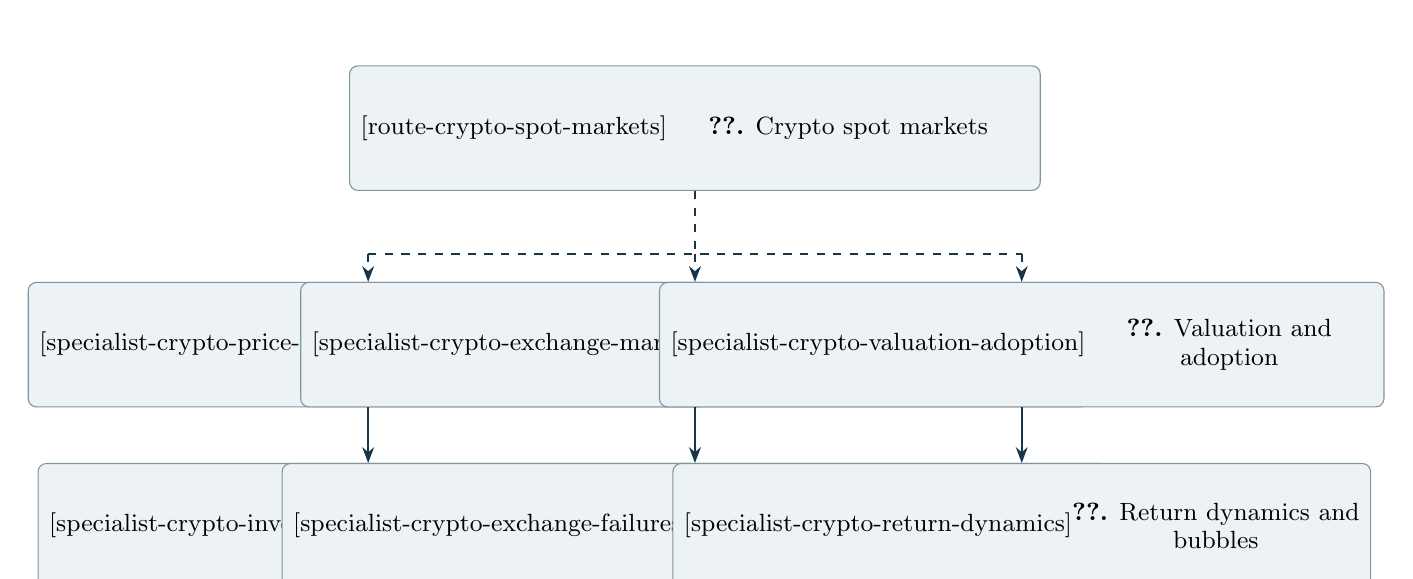
\begin{tikzpicture}[x=1cm,y=1cm]
\node[pathnode] (crypto-spot-markets) at (4.15,0) {\MeasurePathNode{4.6cm}{\textbf{\ref*{route-crypto-spot-markets}.} Crypto spot markets}\hyperref[route-crypto-spot-markets]{\parbox[c][\pathnodeheight][c]{4.6cm}{\centering \textbf{\ref*{route-crypto-spot-markets}.} Crypto spot markets}}};
\node[pathnode] (crypto-price-discovery) at (0.00,-2.75) {\MeasurePathNode{3.65cm}{\textbf{\ref*{specialist-crypto-price-discovery}.} Price discovery and reference rates}\hyperref[specialist-crypto-price-discovery]{\parbox[c][\pathnodeheight][c]{3.65cm}{\centering \textbf{\ref*{specialist-crypto-price-discovery}.} Price discovery and reference rates}}};
\node[pathnode] (crypto-exchange-market-quality) at (4.15,-2.75) {\MeasurePathNode{3.65cm}{\textbf{\ref*{specialist-crypto-exchange-market-quality}.} Liquidity, fake volume and manipulation}\hyperref[specialist-crypto-exchange-market-quality]{\parbox[c][\pathnodeheight][c]{3.65cm}{\centering \textbf{\ref*{specialist-crypto-exchange-market-quality}.} Liquidity, fake volume and manipulation}}};
\node[pathnode] (crypto-valuation-adoption) at (8.30,-2.75) {\MeasurePathNode{3.65cm}{\textbf{\ref*{specialist-crypto-valuation-adoption}.} Valuation and adoption}\hyperref[specialist-crypto-valuation-adoption]{\parbox[c][\pathnodeheight][c]{3.65cm}{\centering \textbf{\ref*{specialist-crypto-valuation-adoption}.} Valuation and adoption}}};
\node[pathnode] (crypto-investors-etfs) at (0.00,-5.05) {\MeasurePathNode{3.65cm}{\textbf{\ref*{specialist-crypto-investors-etfs}.} Investors and spot ETFs}\hyperref[specialist-crypto-investors-etfs]{\parbox[c][\pathnodeheight][c]{3.65cm}{\centering \textbf{\ref*{specialist-crypto-investors-etfs}.} Investors and spot ETFs}}};
\node[pathnode] (crypto-exchange-failures-regulation) at (4.15,-5.05) {\MeasurePathNode{3.65cm}{\textbf{\ref*{specialist-crypto-exchange-failures-regulation}.} Exchange failures and regulation}\hyperref[specialist-crypto-exchange-failures-regulation]{\parbox[c][\pathnodeheight][c]{3.65cm}{\centering \textbf{\ref*{specialist-crypto-exchange-failures-regulation}.} Exchange failures and regulation}}};
\node[pathnode] (crypto-return-dynamics) at (8.30,-5.05) {\MeasurePathNode{3.65cm}{\textbf{\ref*{specialist-crypto-return-dynamics}.} Return dynamics and bubbles}\hyperref[specialist-crypto-return-dynamics]{\parbox[c][\pathnodeheight][c]{3.65cm}{\centering \textbf{\ref*{specialist-crypto-return-dynamics}.} Return dynamics and bubbles}}};
\draw[entryline] (crypto-spot-markets.south) -- (4.15,-1.60);
\draw[entryline] (0.00,-1.60) -- (8.30,-1.60);
\draw[entryarrow] (0.00,-1.60) -- (crypto-price-discovery.north);
\draw[entryarrow] (4.15,-1.60) -- (crypto-exchange-market-quality.north);
\draw[entryarrow] (8.30,-1.60) -- (crypto-valuation-adoption.north);
\draw[patharrow] (crypto-price-discovery.south) -- (crypto-investors-etfs.north);
\draw[patharrow] (crypto-exchange-market-quality.south) -- (crypto-exchange-failures-regulation.north);
\draw[patharrow] (crypto-valuation-adoption.south) -- (crypto-return-dynamics.north);
\end{tikzpicture}\end{center}
\textbf{Overview checkpoint.} A section capstone: complete it after \hyperref[specialist-crypto-price-discovery]{\ref*{specialist-crypto-price-discovery}} and \hyperref[specialist-crypto-exchange-market-quality]{\ref*{specialist-crypto-exchange-market-quality}}.

\textbf{Bring these foundations with you.}\begin{itemize}
\item \hyperref[specialist-time-series-volatility]{Time-series econometrics and volatility forecasting} --- needed by \hyperref[specialist-crypto-price-discovery]{Price discovery and reference rates}, \hyperref[specialist-crypto-return-dynamics]{Return dynamics and bubbles}.
\item \hyperref[route-execution-market-making]{Market microstructure and market making} --- needed by \hyperref[specialist-crypto-exchange-market-quality]{Liquidity, fake volume and manipulation}.
\end{itemize}\hyperref[learning-map]{Return to the whole-guide DAG.}
\Needspace{12\baselineskip}
\subsection{Crypto price discovery: cross-exchange arbitrage, futures, spot ETFs and reference rates}\label{specialist-crypto-price-discovery}
\textbf{Specialist pathway.} In \hyperref[route-crypto-spot-markets]{Crypto spot markets: price discovery, market quality, valuation and investors}.

\textbf{Outcome.} Measure which exchanges and instruments lead the price of a crypto asset, explain why cross-exchange price gaps persist, and reconstruct the reference rates that settle futures and value funds.

\textbf{Prerequisites.} Crypto spot markets overview; time-series econometrics, including cointegration, for information shares. Futures basis from Crypto perpetuals and cross-venue basis (30.2) helps.

\textbf{Review first.} \hyperref[route-crypto-spot-markets]{Crypto spot markets: price discovery, market quality, valuation and investors}; \hyperref[specialist-time-series-volatility]{Time-series econometrics and volatility forecasting}.

\textbf{Required readings, in order}
\begin{enumerate}\raggedright
\Needspace{5\baselineskip}\item \href{institutional_quantitative_finance_reading_list.pdf\#cs-makarov-schoar-2019}{Igor Makarov and Antoinette Schoar, ``Price Discovery in Cryptocurrency Markets''}\CataloguePage{451}\NoteKey{cs-makarov-schoar-2019}\par \textbf{Evidence.} See how price leadership shifts between exchanges as markets integrate and segment.
\Needspace{5\baselineskip}\item \href{institutional_quantitative_finance_reading_list.pdf\#cs-brandvold-2015}{Morten Brandvold, Peter Molnár, Kristian Vagstad and Ole Christian Andreas Valstad, ``Price discovery on Bitcoin exchanges''}\CataloguePage{451}\NoteKey{cs-brandvold-2015}\par \textbf{Methods.} Estimate information shares across exchanges and expect leadership to change over time.
\Needspace{5\baselineskip}\item \href{institutional_quantitative_finance_reading_list.pdf\#cs-dimpfl-peter-2021}{Thomas Dimpfl and Franziska J. Peter, ``Nothing but noise? Price discovery across cryptocurrency exchanges''}\CataloguePage{451}\NoteKey{cs-dimpfl-peter-2021}\par \textbf{Methods.} Correct price-discovery measures for the heavy microstructure noise of crypto venues.
\Needspace{5\baselineskip}\item \href{institutional_quantitative_finance_reading_list.pdf\#catalogue-0829}{Nicola Borri and Kirill Shakhnov, ``The Cross-Section of Cryptocurrency Returns''}\CataloguePage{451}\NoteKey{catalogue-0829}\par \textbf{Evidence.} Read cross-exchange and cross-currency price differences as compensation for liquidity and sentiment risk.
\Needspace{5\baselineskip}\item \href{institutional_quantitative_finance_reading_list.pdf\#cs-hautsch-2024}{Nikolaus Hautsch, Christoph Scheuch and Stefan Voigt, ``Building trust takes time: limits to arbitrage for blockchain-based assets''}\CataloguePage{451}\NoteKey{cs-hautsch-2024}\par \textbf{Theory.} Link arbitrage spreads to settlement latency and exchange default risk.
\Needspace{5\baselineskip}\item \href{institutional_quantitative_finance_reading_list.pdf\#cs-krueckeberg-scholz-2020}{Sinan Krückeberg and Peter Scholz, ``Decentralized Efficiency? Arbitrage in Bitcoin Markets''}\CataloguePage{452}\NoteKey{cs-krueckeberg-scholz-2020}\par \textbf{Evidence.} Document the size and timing of pre-2018 arbitrage spreads.
\Needspace{5\baselineskip}\item \href{institutional_quantitative_finance_reading_list.pdf\#cs-crepelliere-2023}{Tommy Crépellière, Matthias Pelster and Stefan Zeisberger, ``Arbitrage in the market for cryptocurrencies''}\CataloguePage{452}\NoteKey{cs-crepelliere-2023}\par \textbf{Counter-evidence.} Check how far arbitrage opportunities shrank after April 2018 and whether they survive costs.
\Needspace{5\baselineskip}\item \href{institutional_quantitative_finance_reading_list.pdf\#cs-augustin-2023}{Patrick Augustin, Alexey Rubtsov and Donghwa Shin, ``The Impact of Derivatives on Spot Markets: Evidence from the Introduction of Bitcoin Futures Contracts''}\CataloguePage{452}\NoteKey{cs-augustin-2023}\par \textbf{Evidence.} Use the 2017 futures launch to see how derivatives changed spot price efficiency and liquidity.
\Needspace{5\baselineskip}\item \href{institutional_quantitative_finance_reading_list.pdf\#cs-baur-dimpfl-2019}{Dirk G. Baur and Thomas Dimpfl, ``Price discovery in bitcoin spot or futures?''}\CataloguePage{452}\NoteKey{cs-baur-dimpfl-2019}\par \textbf{Evidence.} Compare spot and futures leadership in the early CME and CBOE period.
\Needspace{5\baselineskip}\item \href{institutional_quantitative_finance_reading_list.pdf\#cs-aleti-mizrach-2021}{Saketh Aleti and Bruce Mizrach, ``Bitcoin spot and futures market microstructure''}\CataloguePage{452}\NoteKey{cs-aleti-mizrach-2021}\par \textbf{Counter-evidence.} Contrast CME and spot-exchange microstructure and the later evidence that the CME leads.
\Needspace{5\baselineskip}\item \href{institutional_quantitative_finance_reading_list.pdf\#cs-mohamad-2025}{Azhar Mohamad, ``Do Bitcoin ETFs Lead Price Discovery Following their Introduction in the Bitcoin Market?''}\CataloguePage{453}\NoteKey{cs-mohamad-2025}\par \textbf{Evidence.} Test whether spot ETFs now lead spot bitcoin during US trading hours.
\Needspace{5\baselineskip}\item \href{institutional_quantitative_finance_reading_list.pdf\#cs-cfb-reference-rates-2026}{CF Benchmarks, CME CF Cryptocurrency Reference Rates: Methodology Guide; Constituent Exchanges List}\CataloguePage{453}\NoteKey{cs-cfb-reference-rates-2026}\par\emph{Selection:} Sections 2--5 (overview, definitions, methodology and contingency rules) and the constituent-exchange list.\par \textbf{Mechanics.} Reconstruct the volume-weighted-median reference rate that settles futures and anchors fund valuation.
\end{enumerate}
\Needspace{5\baselineskip}\textbf{Checkpoint.} For BTC--USD and BTC--USDT on four exchanges and the front CME future over one week that includes a volatility spike, estimate Hasbrouck information shares and information leadership shares at one-minute and five-second sampling, and report how the ranking changes with sampling and noise. Compute cross-exchange spreads net of fees, withdrawal time and confirmation delay and say which gaps were executable. Recompute one reference-rate window from constituent-exchange trades and compare it with the published value.

\textbf{Optional branches.} \href{institutional_quantitative_finance_reading_list.pdf\#cs-alexander-2020}{Compare evidence that offshore BitMEX derivatives led spot prices.}\BranchPage{452} \href{institutional_quantitative_finance_reading_list.pdf\#cs-hu-hou-oxley-2020}{Use time-varying causality and information shares on the spot--futures question.}\BranchPage{452} \href{institutional_quantitative_finance_reading_list.pdf\#cs-hattori-ishida-2021}{Reconstruct executable cash-and-carry arbitrage and why it appears in crashes.}\BranchPage{453} \href{institutional_quantitative_finance_reading_list.pdf\#s11-r02}{Survey the crypto microstructure literature by research strand.}\BranchPage{451} \href{institutional_quantitative_finance_reading_list.pdf\#w3-albers-latency-crypto}{Measure how latency changes execution against order-book snapshots.}\BranchPage{454}
\par{\small \hyperref[learning-map]{Learning pathway DAG} \textbar{} \hyperref[route-crypto-spot-markets]{Section overview} \textbar{} \hyperref[map-crypto-spot-markets]{Section DAG}\NoteKey{crypto-price-discovery}}
\Needspace{12\baselineskip}
\subsection{Crypto exchange market quality: liquidity, fake volume and manipulation}\label{specialist-crypto-exchange-market-quality}
\textbf{Specialist pathway.} In \hyperref[route-crypto-spot-markets]{Crypto spot markets: price discovery, market quality, valuation and investors}.

\textbf{Outcome.} Measure liquidity and trading costs on crypto exchanges, test reported volume for wash trading, and recognise the main manipulation patterns: exchange self-dealing, stablecoin-funded buying and pump-and-dump schemes.

\textbf{Prerequisites.} Crypto spot markets overview; Market microstructure and market making for spreads, depth and adverse selection.

\textbf{Review first.} \hyperref[route-crypto-spot-markets]{Crypto spot markets: price discovery, market quality, valuation and investors}; \hyperref[route-execution-market-making]{Market microstructure and market making}.

\textbf{Required readings, in order}
\begin{enumerate}\raggedright
\Needspace{5\baselineskip}\item \href{institutional_quantitative_finance_reading_list.pdf\#cs-dyhrberg-2018}{Anne H. Dyhrberg, Sean Foley and Jiri Svec, ``How investible is Bitcoin? Analyzing the liquidity and transaction costs of Bitcoin markets''}\CataloguePage{454}\NoteKey{cs-dyhrberg-2018}\par \textbf{Evidence.} Measure quoted and effective spreads by hour and compare crypto with equity trading costs.
\Needspace{5\baselineskip}\item \href{institutional_quantitative_finance_reading_list.pdf\#cs-brauneis-2021}{Alexander Brauneis, Roland Mestel, Ryan Riordan and Erik Theissen, ``How to measure the liquidity of cryptocurrency markets?''}\CataloguePage{454}\NoteKey{cs-brauneis-2021}\par \textbf{Methods.} Choose low-frequency liquidity measures that track high-frequency liquidity on crypto venues.
\Needspace{5\baselineskip}\item \href{institutional_quantitative_finance_reading_list.pdf\#catalogue-0828}{Peter Reinhard Hansen, Chan Kim and Wade Kimbrough, ``Periodicity in Cryptocurrency Volatility and Liquidity''}\CataloguePage{453}\NoteKey{catalogue-0828}\par \textbf{Evidence.} Map daily and intraday periodicity in crypto volatility and volume on centralised and decentralised exchanges.
\Needspace{5\baselineskip}\item \href{institutional_quantitative_finance_reading_list.pdf\#wide-cong-wash-trading}{Lin William Cong, Xi Li, Ke Tang and Yang Yang, ``Crypto Wash Trading''}\CataloguePage{453}\NoteKey{wide-cong-wash-trading}\par \textbf{Methods.} Apply Benford, trade-size clustering and other statistical tests for wash trading.
\Needspace{5\baselineskip}\item \href{institutional_quantitative_finance_reading_list.pdf\#cs-aloosh-li-2024}{Arash Aloosh and Jiasun Li, ``Direct Evidence of Bitcoin Wash Trading''}\CataloguePage{454}\NoteKey{cs-aloosh-li-2024}\par \textbf{Validation.} Validate indirect wash-trading tests against direct evidence from leaked exchange records.
\Needspace{5\baselineskip}\item \href{institutional_quantitative_finance_reading_list.pdf\#cs-amiram-2025}{Dan Amiram, Evgeny Lyandres and Daniel Rabetti, ``Trading Volume Manipulation and Competition Among Centralized Crypto Exchanges''}\CataloguePage{454}\NoteKey{cs-amiram-2025}\par \textbf{Evidence.} Explain why competing exchanges inflate volume and what it costs them later.
\Needspace{5\baselineskip}\item \href{institutional_quantitative_finance_reading_list.pdf\#cs-gandal-2018}{Neil Gandal, J. T. Hamrick, Tyler Moore and Tali Oberman, ``Price manipulation in the Bitcoin ecosystem''}\CataloguePage{454}\NoteKey{cs-gandal-2018}\par \textbf{Evidence.} Trace how suspicious trading on one exchange moved the market price in 2013.
\Needspace{5\baselineskip}\item \href{institutional_quantitative_finance_reading_list.pdf\#wide-griffin-shams-tether}{John M. Griffin and Amin Shams, ``Is Bitcoin Really Untethered?''}\CataloguePage{453}\NoteKey{wide-griffin-shams-tether}\par \textbf{Evidence.} Test whether stablecoin issuance was used to support prices after market falls.
\Needspace{5\baselineskip}\item \href{institutional_quantitative_finance_reading_list.pdf\#w3-li-shin-wang-pump-dump}{Tao Li, Donghwa Shin and Baolian Wang, ``Cryptocurrency Pump-and-Dump Schemes''}\CataloguePage{453}\NoteKey{w3-li-shin-wang-pump-dump}\par \textbf{Evidence.} Document pump-and-dump schemes, their run-ups and wealth transfers.
\Needspace{5\baselineskip}\item \href{institutional_quantitative_finance_reading_list.pdf\#cs-dhawan-putnins-2023}{Anirudh Dhawan and Tālis J. Putniņš, ``A New Wolf in Town? Pump-and-Dump Manipulation in Cryptocurrency Markets''}\CataloguePage{455}\NoteKey{cs-dhawan-putnins-2023}\par \textbf{Theory.} Explain why traders join announced pumps despite negative expected returns.
\end{enumerate}
\Needspace{5\baselineskip}\textbf{Checkpoint.} Take one month of trades and order-book snapshots for one pair on a regulated exchange and on an unregulated exchange. Compute quoted, effective and Abdi--Ranaldo spreads by hour of day; apply Benford, trade-size clustering and round-number tests to trade sizes; and estimate how much of the unregulated venue's reported volume survives. For one announced pump, measure price, volume and order imbalance from an hour before to a day after, and estimate who bought at the peak.

\textbf{Optional branches.} \href{institutional_quantitative_finance_reading_list.pdf\#cs-brauneis-2022-drivers}{Relate crypto liquidity to volatility, volume and trade counts over four years.}\BranchPage{454} \href{institutional_quantitative_finance_reading_list.pdf\#cs-lepennec-2021}{Estimate true exchange volume from web traffic and user funds.}\BranchPage{455} \href{institutional_quantitative_finance_reading_list.pdf\#cs-hamrick-2021}{Measure the pump-and-dump ecosystem on messaging platforms.}\BranchPage{455} \href{institutional_quantitative_finance_reading_list.pdf\#w5-barbon-ranaldo-quality}{Compare market quality on centralised and decentralised venues.}\BranchPage{477} \href{institutional_quantitative_finance_reading_list.pdf\#s11-r27}{Treat exchange-level data quality and provider dependence before any market-quality comparison.}\BranchPage{476}
\par{\small \hyperref[learning-map]{Learning pathway DAG} \textbar{} \hyperref[route-crypto-spot-markets]{Section overview} \textbar{} \hyperref[map-crypto-spot-markets]{Section DAG}\NoteKey{crypto-exchange-market-quality}}
\Needspace{12\baselineskip}
\subsection{Bitcoin and token valuation: monetary models, adoption, mining and equilibrium prices}\label{specialist-crypto-valuation-adoption}
\textbf{Specialist pathway.} In \hyperref[route-crypto-spot-markets]{Crypto spot markets: price discovery, market quality, valuation and investors}.

\textbf{Outcome.} Explain what equilibrium models say a cryptocurrency or platform token is worth, why they admit multiple equilibria and sunspots, and how adoption, transaction fees, security and mining shape the price.

\textbf{Prerequisites.} Crypto spot markets overview; basic monetary and asset-pricing theory (overlapping generations, martingale pricing).

\textbf{Review first.} \hyperref[route-crypto-spot-markets]{Crypto spot markets: price discovery, market quality, valuation and investors}.

\textbf{Required readings, in order}
\begin{enumerate}\raggedright
\Needspace{5\baselineskip}\item \href{institutional_quantitative_finance_reading_list.pdf\#cs-yermack-2015}{David Yermack, ``Is Bitcoin a Real Currency? An Economic Appraisal''}\CataloguePage{455}\NoteKey{cs-yermack-2015}\par \textbf{Foundations.} Test bitcoin against the three functions of money before modelling its value.
\Needspace{5\baselineskip}\item \href{institutional_quantitative_finance_reading_list.pdf\#cs-garratt-wallace-2018}{Rodney Garratt and Neil Wallace, ``Bitcoin 1, Bitcoin 2, \ldots: An Experiment in Privately Issued Outside Monies''}\CataloguePage{456}\NoteKey{cs-garratt-wallace-2018}\par \textbf{Theory.} See why the value of an intrinsically worthless private money is indeterminate.
\Needspace{5\baselineskip}\item \href{institutional_quantitative_finance_reading_list.pdf\#cs-schilling-uhlig-2019}{Linda Schilling and Harald Uhlig, ``Some simple bitcoin economics''}\CataloguePage{456}\NoteKey{cs-schilling-uhlig-2019}\par \textbf{Theory.} Derive martingale bitcoin prices in a two-currency economy.
\Needspace{5\baselineskip}\item \href{institutional_quantitative_finance_reading_list.pdf\#wide-biais-bitcoin-pricing}{Bruno Biais, Christophe Bisière, Matthieu Bouvard, Catherine Casamatta and Albert J. Menkveld, ``Equilibrium Bitcoin Pricing''}\CataloguePage{455}\NoteKey{wide-biais-bitcoin-pricing}\par \textbf{Valuation.} Value bitcoin as a stream of net transactional benefits and estimate how much of its volatility is extrinsic.
\Needspace{5\baselineskip}\item \href{institutional_quantitative_finance_reading_list.pdf\#cs-pagnotta-2022}{Emiliano S. Pagnotta, ``Decentralizing Money: Bitcoin Prices and Blockchain Security''}\CataloguePage{456}\NoteKey{cs-pagnotta-2022}\par \textbf{Valuation.} Price bitcoin jointly with blockchain security and see how the feedback creates booms and busts.
\Needspace{5\baselineskip}\item \href{institutional_quantitative_finance_reading_list.pdf\#cs-sockin-xiong-2023}{Michael Sockin and Wei Xiong, ``A Model of Cryptocurrencies''}\CataloguePage{456}\NoteKey{cs-sockin-xiong-2023}\par \textbf{Theory.} Model platform tokens with network effects and see when the token market breaks down.
\Needspace{5\baselineskip}\item \href{institutional_quantitative_finance_reading_list.pdf\#roadmap-tokenomics}{Lin William Cong, Ye Li and Neng Wang, Tokenomics: Dynamic Adoption and Valuation; NBER working paper}\CataloguePage{484}\NoteKey{roadmap-tokenomics}\par \textbf{Valuation.} Value tokens through dynamic user adoption on a platform.
\Needspace{5\baselineskip}\item \href{institutional_quantitative_finance_reading_list.pdf\#cs-huberman-2021}{Gur Huberman, Jacob D. Leshno and Ciamac Moallemi, ``Monopoly without a Monopolist: An Economic Analysis of the Bitcoin Payment System''}\CataloguePage{456}\NoteKey{cs-huberman-2021}\par \textbf{Theory.} Derive transaction fees and waiting times in a decentralised payment system.
\Needspace{5\baselineskip}\item \href{institutional_quantitative_finance_reading_list.pdf\#cs-prat-walter-2021}{Julien Prat and Benjamin Walter, ``An Equilibrium Model of the Market for Bitcoin Mining''}\CataloguePage{456}\NoteKey{cs-prat-walter-2021}\par \textbf{Evidence.} Show that mining capacity follows the price through free entry.
\Needspace{5\baselineskip}\item \href{institutional_quantitative_finance_reading_list.pdf\#cs-bolt-vanoordt-2020}{Wilko Bolt and Maarten R. C. van Oordt, ``On the Value of Virtual Currencies''}\CataloguePage{456}\NoteKey{cs-bolt-vanoordt-2020}\par \textbf{Theory.} Decompose a virtual currency's exchange rate into transactional use, speculation and expected adoption.
\end{enumerate}
\Needspace{5\baselineskip}\textbf{Checkpoint.} Calibrate either Biais et al. or Schilling and Uhlig to bitcoin data: on-chain transaction value, the block-reward schedule, fees and hash rate. Report the price path or fundamental value the model implies and the share of observed volatility it leaves unexplained. Use Prat and Walter to predict next quarter's hash rate from the price and compare it with the outcome, and state which assumption (transaction benefit, attack risk or adoption) moves the valuation most.

\textbf{Optional branches.} \href{institutional_quantitative_finance_reading_list.pdf\#cs-gandal-halaburda-2016}{Look for network effects and winner-take-all dynamics among early cryptocurrencies.}\BranchPage{456} \href{institutional_quantitative_finance_reading_list.pdf\#cs-cong-he-li-2021}{Study how mining pools affect decentralisation and energy use.}\BranchPage{457} \href{institutional_quantitative_finance_reading_list.pdf\#wide-budish-bitcoin-limits}{Study the economic limits of Nakamoto consensus.}\BranchPage{437} \href{institutional_quantitative_finance_reading_list.pdf\#s6-easley}{Link mining costs, fees and transaction waiting times to markets.}\BranchPage{439} \href{institutional_quantitative_finance_reading_list.pdf\#w6-cong-li-wang-platform}{Model token-financed platforms.}\BranchPage{484} \href{institutional_quantitative_finance_reading_list.pdf\#cs-bis-aer-2018}{Read the central banks' case that cryptocurrencies cannot work as money.}\BranchPage{457}
\par{\small \hyperref[learning-map]{Learning pathway DAG} \textbar{} \hyperref[route-crypto-spot-markets]{Section overview} \textbar{} \hyperref[map-crypto-spot-markets]{Section DAG}\NoteKey{crypto-valuation-adoption}}
\Needspace{12\baselineskip}
\subsection{Crypto investors and access: retail trading, spot ETFs and bank custody}\label{specialist-crypto-investors-etfs}
\textbf{Specialist pathway.} In \hyperref[route-crypto-spot-markets]{Crypto spot markets: price discovery, market quality, valuation and investors}.

\textbf{Outcome.} Describe who buys crypto and how their demand responds to prices, income and information; explain how spot ETFs were approved and how their flows relate to prices; and identify the rules that set the cost to banks of holding and custodying crypto.

\textbf{Prerequisites.} Crypto price discovery (31.1). ETF creation, redemption and closing-auction mechanics from ETFs, index events and closing auctions help.

\textbf{Review first.} \hyperref[specialist-crypto-price-discovery]{Crypto price discovery: cross-exchange arbitrage, futures, spot ETFs and reference rates}.

\textbf{Required readings, in order}
\begin{enumerate}\raggedright
\Needspace{5\baselineskip}\item \href{institutional_quantitative_finance_reading_list.pdf\#cs-kogan-2024}{Shimon Kogan, Igor Makarov, Marina Niessner and Antoinette Schoar, ``Are cryptos different? Evidence from retail trading''}\CataloguePage{460}\NoteKey{cs-kogan-2024}\par \textbf{Evidence.} Compare the same retail traders' behaviour in crypto, stocks and gold.
\Needspace{5\baselineskip}\item \href{institutional_quantitative_finance_reading_list.pdf\#cs-auer-2025}{Raphael Auer, Giulio Cornelli, Sebastian Doerr, Jon Frost and Leonardo Gambacorta, ``Crypto Trading and Bitcoin Prices: Evidence from a New Database of Retail Adoption''}\CataloguePage{460}\NoteKey{cs-auer-2025}\par \textbf{Evidence.} See who enters after price rises and who sells to them, across 95 countries.
\Needspace{5\baselineskip}\item \href{institutional_quantitative_finance_reading_list.pdf\#cs-divakaruni-2023}{Anantha Divakaruni and Peter Zimmerman, ``Uncovering Retail Trading in Bitcoin: The Impact of COVID-19 Stimulus Checks''}\CataloguePage{460}\NoteKey{cs-divakaruni-2023}\par \textbf{Evidence.} Use stimulus payments to measure retail demand for bitcoin and its price elasticity.
\Needspace{5\baselineskip}\item \href{institutional_quantitative_finance_reading_list.pdf\#cs-hackethal-2022}{Andreas Hackethal, Tobin Hanspal, Dominique M. Lammer and Kevin Rink, ``The Characteristics and Portfolio Behavior of Bitcoin Investors: Evidence from Indirect Cryptocurrency Investments''}\CataloguePage{460}\NoteKey{cs-hackethal-2022}\par \textbf{Evidence.} Profile investors who buy crypto exposure through retail products.
\Needspace{5\baselineskip}\item \href{institutional_quantitative_finance_reading_list.pdf\#cs-aiello-2023}{Darren Aiello, Scott R. Baker, Tetyana Balyuk, Marco Di Maggio, Mark J. Johnson and Jason D. Kotter, ``Who Invests in Crypto? Wealth, Financial Constraints, and Risk Attitudes''}\CataloguePage{461}\NoteKey{cs-aiello-2023}\par \textbf{Evidence.} Use household transaction data on who invests in crypto and what triggers purchases.
\Needspace{5\baselineskip}\item \href{institutional_quantitative_finance_reading_list.pdf\#cs-sec-bitcoin-etp-2024}{U.S. Securities and Exchange Commission, Order Granting Accelerated Approval of Proposed Rule Changes \ldots\ to List and Trade Bitcoin-Based Commodity-Based Trust Shares and Trust Units (Release 34-99306)}\CataloguePage{461}\NoteKey{cs-sec-bitcoin-etp-2024}\par \textbf{Regulation.} Follow the surveillance-sharing and correlation analysis behind the 2024 approval of spot bitcoin ETPs.
\Needspace{5\baselineskip}\item \href{institutional_quantitative_finance_reading_list.pdf\#w4-hornback-whaley-bitcoin-etf}{Andrew M. Hornback and Robert E. Whaley, ``Spot Bitcoin ETFs: The Struggle Was Worth It''}\CataloguePage{460}\NoteKey{w4-hornback-whaley-bitcoin-etf}\par \textbf{Evidence.} Compare first-year spot ETF performance with futures and futures-based funds.
\Needspace{5\baselineskip}\item \href{institutional_quantitative_finance_reading_list.pdf\#cs-mazur-polyzos-2025}{Mieszko Mazur and Efstathios Polyzos, ``Spot Bitcoin ETFs: The Effect of Fund Flows on Bitcoin Price Formation''}\CataloguePage{461}\NoteKey{cs-mazur-polyzos-2025}\par \textbf{Evidence.} Relate daily ETF flows to bitcoin prices and to trading hours.
\Needspace{5\baselineskip}\item \href{institutional_quantitative_finance_reading_list.pdf\#cs-sec-generic-listing-2025}{U.S. Securities and Exchange Commission, Order Granting Accelerated Approval \ldots\ to Adopt Generic Listing Standards for Commodity-Based Trust Shares (Release 34-103995)}\CataloguePage{461}\NoteKey{cs-sec-generic-listing-2025}\par \textbf{Regulation.} Apply the 2025 generic listing criteria that decide which other tokens can get spot ETPs.
\Needspace{5\baselineskip}\item \href{institutional_quantitative_finance_reading_list.pdf\#cs-bcbs-cryptoasset-2022}{Basel Committee on Banking Supervision, Prudential Treatment of Cryptoasset Exposures (SCO60); Cryptoasset standard amendments (July 2024); February 2026 review update}\CataloguePage{462}\NoteKey{cs-bcbs-cryptoasset-2022}\par \textbf{Regulation.} Identify how the Basel standard prices bank exposure to stablecoins and unbacked crypto.
\end{enumerate}
\Needspace{5\baselineskip}\textbf{Checkpoint.} For one spot bitcoin ETF over three months, reconcile daily creations and redemptions and bitcoin holdings with NAV and the reference rate it names; measure the premium or discount at the close and at the next open, and relate daily net flows to bitcoin returns overnight and during US hours. Contrast the result with one retail cohort from Kogan et al. or Auer et al.: who buys after price rises, who sells, and what this implies for the flow--return relation.

\textbf{Optional branches.} \href{institutional_quantitative_finance_reading_list.pdf\#cs-weber-2023}{Use household surveys on crypto holders' beliefs and spending.}\BranchPage{461} \href{institutional_quantitative_finance_reading_list.pdf\#cs-pelster-2019}{See whether crypto traders become more risk-seeking in stocks.}\BranchPage{460} \href{institutional_quantitative_finance_reading_list.pdf\#cs-hasso-2019}{Profile brokerage-account crypto traders by demographics and performance.}\BranchPage{460} \href{institutional_quantitative_finance_reading_list.pdf\#cs-babalos-2025}{Measure return and volatility effects of the spot ETF launch.}\BranchPage{461} \href{institutional_quantitative_finance_reading_list.pdf\#roadmap-bitcoin-entities}{Measure concentration of bitcoin holdings from blockchain entity analysis.}\BranchPage{475} \href{institutional_quantitative_finance_reading_list.pdf\#subsection.8.8.3}{Review ETF creation, redemption and closing-auction mechanics.}\BranchPage{175}
\par{\small \hyperref[learning-map]{Learning pathway DAG} \textbar{} \hyperref[route-crypto-spot-markets]{Section overview} \textbar{} \hyperref[map-crypto-spot-markets]{Section DAG}\NoteKey{crypto-investors-etfs}}
\Needspace{12\baselineskip}
\subsection{Crypto exchange failures, customer assets and market regulation}\label{specialist-crypto-exchange-failures-regulation}
\textbf{Specialist pathway.} In \hyperref[route-crypto-spot-markets]{Crypto spot markets: price discovery, market quality, valuation and investors}.

\textbf{Outcome.} Assess the counterparty risk of a crypto exchange from its custody, governance and affiliations; explain what proofs of reserves can and cannot show; and map the international and US rules that apply to trading platforms and their market reactions.

\textbf{Prerequisites.} Crypto exchange market quality (31.2). Stablecoins and tokenised bonds (30.1) helps for stablecoin runs and reserves.

\textbf{Review first.} \hyperref[specialist-crypto-exchange-market-quality]{Crypto exchange market quality: liquidity, fake volume and manipulation}.

\textbf{Required readings, in order}
\begin{enumerate}\raggedright
\Needspace{5\baselineskip}\item \href{institutional_quantitative_finance_reading_list.pdf\#cs-moore-christin-2013}{Tyler Moore and Nicolas Christin, ``Beware the Middleman: Empirical Analysis of Bitcoin-Exchange Risk''}\CataloguePage{462}\NoteKey{cs-moore-christin-2013}\par \textbf{Evidence.} Measure how often exchanges close or are breached and what predicts it.
\Needspace{5\baselineskip}\item \href{institutional_quantitative_finance_reading_list.pdf\#cs-dagher-2015}{Gaby G. Dagher, Benedikt Bünz, Joseph Bonneau, Jeremy Clark and Dan Boneh, ``Provisions: Privacy-preserving Proofs of Solvency for Bitcoin Exchanges''}\CataloguePage{462}\NoteKey{cs-dagher-2015}\par \textbf{Methods.} Design a proof of solvency that covers liabilities as well as reserves.
\Needspace{5\baselineskip}\item \href{institutional_quantitative_finance_reading_list.pdf\#cs-ftx-ray-2023}{John J. Ray III, First Interim Report of John J. Ray III to the Independent Directors on Control Failures at the FTX Exchanges}\CataloguePage{462}\NoteKey{cs-ftx-ray-2023}\par\emph{Selection:} Sections I and IV.\par \textbf{Evidence.} Read the control failures behind the FTX collapse in the debtors' own report.
\Needspace{5\baselineskip}\item \href{institutional_quantitative_finance_reading_list.pdf\#cs-vidal-tomas-2023}{David Vidal-Tomás, Antonio Briola and Tomaso Aste, ``FTX's downfall and Binance's consolidation: The fragility of centralised digital finance''}\CataloguePage{462}\NoteKey{cs-vidal-tomas-2023}\par \textbf{Evidence.} Trace FTX's use of its own token and the on-chain run on the exchange.
\Needspace{5\baselineskip}\item \href{institutional_quantitative_finance_reading_list.pdf\#cs-galati-2024}{Luca Galati, Alexander Webb and Robert I. Webb, ``Financial contagion in cryptocurrency exchanges: Evidence from the FTT collapse''}\CataloguePage{463}\NoteKey{cs-galati-2024}\par \textbf{Evidence.} Measure contagion across exchanges when FTX froze withdrawals.
\Needspace{5\baselineskip}\item \href{institutional_quantitative_finance_reading_list.pdf\#cs-fsb-mci-2023}{Financial Stability Board, The Financial Stability Implications of Multifunction Crypto-asset Intermediaries}\CataloguePage{463}\NoteKey{cs-fsb-mci-2023}\par \textbf{Regulation.} Identify the vulnerabilities created by combining exchange, custody, lending and trading in one group.
\Needspace{5\baselineskip}\item \href{institutional_quantitative_finance_reading_list.pdf\#cs-auer-claessens-2018}{Raphael Auer and Stijn Claessens, ``Regulating cryptocurrencies: assessing market reactions'' (BIS Quarterly Review, September 2018)}\CataloguePage{463}\NoteKey{cs-auer-claessens-2018}\par \textbf{Evidence.} Measure how different kinds of regulatory news move crypto prices.
\Needspace{5\baselineskip}\item \href{institutional_quantitative_finance_reading_list.pdf\#cs-feinstein-werbach-2021}{Brian D. Feinstein and Kevin Werbach, ``The Impact of Cryptocurrency Regulation on Trading Markets''}\CataloguePage{463}\NoteKey{cs-feinstein-werbach-2021}\par \textbf{Counter-evidence.} Test whether regulation drives trading out of a jurisdiction.
\Needspace{5\baselineskip}\item \href{institutional_quantitative_finance_reading_list.pdf\#wide-mica}{European Parliament and Council, ``Regulation (EU) 2023/1114 on markets in crypto-assets (MiCA)''}\CataloguePage{486}\NoteKey{wide-mica}\par\emph{Selection:} Titles V and VI on crypto-asset service providers and market abuse.\par \textbf{Regulation.} Map the EU authorisation, custody and market-abuse rules for crypto-asset service providers.
\Needspace{5\baselineskip}\item \href{institutional_quantitative_finance_reading_list.pdf\#cs-us-spot-crypto-2025}{U.S. Securities and Exchange Commission and Commodity Futures Trading Commission staff, Joint Statement on Trading of Certain Spot Crypto Asset Products; CFTC, First-Ever Listed Spot Crypto Trading on U.S. Regulated Exchanges (Release 9145-25)}\CataloguePage{463}\NoteKey{cs-us-spot-crypto-2025}\par \textbf{Regulation.} Follow how US regulators opened registered exchanges to spot crypto trading in 2025.
\Needspace{5\baselineskip}\item \href{institutional_quantitative_finance_reading_list.pdf\#cs-clarity-act-2026}{United States Congress, H.R. 3633, Digital Asset Market Clarity Act (CLARITY Act)}\CataloguePage{464}\NoteKey{cs-clarity-act-2026}\par \textbf{Regulation.} Read the proposed US market-structure law and why it stalled in September 2026.
\end{enumerate}
\Needspace{5\baselineskip}\textbf{Checkpoint.} Take one failed exchange (Mt.Gox, QuadrigaCX or FTX) and one operating exchange. From public sources, reconstruct each one's customer-asset arrangements: segregation, wallet structure, attestations or proofs of reserves, affiliated trading firms and its own token. Identify which IOSCO custody and conflict recommendations and which MiCA obligations would apply, and design a liability-inclusive proof of solvency for the operating exchange with a list of what it cannot prove.

\textbf{Optional branches.} \href{institutional_quantitative_finance_reading_list.pdf\#cs-moore-2018}{Extend the exchange-closure evidence to 80 exchanges.}\BranchPage{462} \href{institutional_quantitative_finance_reading_list.pdf\#cs-chokor-alfieri-2021}{Measure returns around regulatory events by coin liquidity.}\BranchPage{463} \href{institutional_quantitative_finance_reading_list.pdf\#wide-liu-makarov-schoar-terra}{Analyse the Terra run that preceded FTX's collapse.}\BranchPage{487} \href{institutional_quantitative_finance_reading_list.pdf\#wide-genius-act}{Map the US payment-stablecoin regime that platforms rely on for settlement.}\BranchPage{486}
\par{\small \hyperref[learning-map]{Learning pathway DAG} \textbar{} \hyperref[route-crypto-spot-markets]{Section overview} \textbar{} \hyperref[map-crypto-spot-markets]{Section DAG}\NoteKey{crypto-exchange-failures-regulation}}
\Needspace{12\baselineskip}
\subsection{Crypto return dynamics: volatility, bubbles, efficiency and links to other assets}\label{specialist-crypto-return-dynamics}
\textbf{Specialist pathway.} In \hyperref[route-crypto-spot-markets]{Crypto spot markets: price discovery, market quality, valuation and investors}.

\textbf{Outcome.} Describe crypto return, volatility and jump behaviour, test efficiency and date-stamp bubbles, and measure how crypto co-moves with equities, gold, the dollar and monetary policy, separating robust findings from sample-specific ones.

\textbf{Prerequisites.} Bitcoin and token valuation (31.3); Time-series econometrics and volatility forecasting. Crypto signals and on-chain evidence (32.7) builds a cross-sectional baseline on the same data.

\textbf{Review first.} \hyperref[specialist-crypto-valuation-adoption]{Bitcoin and token valuation: monetary models, adoption, mining and equilibrium prices}; \hyperref[specialist-time-series-volatility]{Time-series econometrics and volatility forecasting}.

\textbf{Required readings, in order}
\begin{enumerate}\raggedright
\Needspace{5\baselineskip}\item \href{institutional_quantitative_finance_reading_list.pdf\#cs-hu-parlour-rajan-2019}{Albert S. Hu, Christine A. Parlour and Uday Rajan, ``Cryptocurrencies: Stylized facts on a new investible instrument''}\CataloguePage{457}\NoteKey{cs-hu-parlour-rajan-2019}\par \textbf{Foundations.} Start from stylised facts on the returns of hundreds of coins.
\Needspace{5\baselineskip}\item \href{institutional_quantitative_finance_reading_list.pdf\#roadmap-crypto-risks-returns}{Yukun Liu and Aleh Tsyvinski, Risks and Returns of Cryptocurrency; NBER working paper 24877}\CataloguePage{442}\NoteKey{roadmap-crypto-risks-returns}\par \textbf{Evidence.} Relate crypto returns to standard factors, momentum and investor attention.
\Needspace{5\baselineskip}\item \href{institutional_quantitative_finance_reading_list.pdf\#cs-urquhart-2016}{Andrew Urquhart, ``The inefficiency of Bitcoin''}\CataloguePage{457}\NoteKey{cs-urquhart-2016}\par \textbf{Evidence.} Test weak-form efficiency of bitcoin returns by sub-period.
\Needspace{5\baselineskip}\item \href{institutional_quantitative_finance_reading_list.pdf\#cs-nadarajah-chu-2017}{Saralees Nadarajah and Jeffrey Chu, ``On the inefficiency of Bitcoin''}\CataloguePage{457}\NoteKey{cs-nadarajah-chu-2017}\par \textbf{Counter-evidence.} See how the efficiency verdict changes with a transformation of returns.
\Needspace{5\baselineskip}\item \href{institutional_quantitative_finance_reading_list.pdf\#cs-cheah-fry-2015}{Eng-Tuck Cheah and John Fry, ``Speculative bubbles in Bitcoin markets? An empirical investigation into the fundamental value of Bitcoin''}\CataloguePage{457}\NoteKey{cs-cheah-fry-2015}\par \textbf{Evidence.} Read the early evidence of speculative bubbles in bitcoin.
\Needspace{5\baselineskip}\item \href{institutional_quantitative_finance_reading_list.pdf\#cs-psy-2015}{Peter C. B. Phillips, Shuping Shi and Jun Yu, ``Testing for Multiple Bubbles: Historical Episodes of Exuberance and Collapse in the S\&P 500''}\CataloguePage{457}\NoteKey{cs-psy-2015}\par \textbf{Methods.} Date-stamp the start and end of multiple bubbles with a recursive right-tailed test.
\Needspace{5\baselineskip}\item \href{institutional_quantitative_finance_reading_list.pdf\#cs-katsiampa-2017}{Paraskevi Katsiampa, ``Volatility estimation for Bitcoin: A comparison of GARCH models''}\CataloguePage{458}\NoteKey{cs-katsiampa-2017}\par \textbf{Methods.} Compare GARCH specifications for bitcoin volatility.
\Needspace{5\baselineskip}\item \href{institutional_quantitative_finance_reading_list.pdf\#cs-scaillet-2020}{Olivier Scaillet, Adrien Treccani and Christopher Trevisan, ``High-Frequency Jump Analysis of the Bitcoin Market''}\CataloguePage{458}\NoteKey{cs-scaillet-2020}\par \textbf{Methods.} Detect jumps in tick data and relate them to order flow and liquidity.
\Needspace{5\baselineskip}\item \href{institutional_quantitative_finance_reading_list.pdf\#cs-conrad-2018}{Christian Conrad, Anessa Custovic and Eric Ghysels, ``Long- and Short-Term Cryptocurrency Volatility Components: A GARCH-MIDAS Analysis''}\CataloguePage{458}\NoteKey{cs-conrad-2018}\par \textbf{Evidence.} Separate long- and short-run bitcoin volatility and link the long run to equity volatility and global activity.
\Needspace{5\baselineskip}\item \href{institutional_quantitative_finance_reading_list.pdf\#cs-baur-hong-lee-2018}{Dirk G. Baur, KiHoon Hong and Adrian D. Lee, ``Bitcoin: Medium of exchange or speculative assets?''}\CataloguePage{458}\NoteKey{cs-baur-hong-lee-2018}\par \textbf{Evidence.} Check whether bitcoin is used and priced as money or as a speculative asset.
\Needspace{5\baselineskip}\item \href{institutional_quantitative_finance_reading_list.pdf\#cs-bouri-2017}{Elie Bouri, Peter Molnár, Georges Azzi, David Roubaud and Lars Ivar Hagfors, ``On the hedge and safe haven properties of Bitcoin: Is it really more than a diversifier?''}\CataloguePage{458}\NoteKey{cs-bouri-2017}\par \textbf{Evidence.} Test hedge and safe-haven properties against equities, bonds, commodities and the dollar.
\Needspace{5\baselineskip}\item \href{institutional_quantitative_finance_reading_list.pdf\#cs-karau-2023}{Sören Karau, ``Monetary policy and Bitcoin''}\CataloguePage{459}\NoteKey{cs-karau-2023}\par \textbf{Evidence.} Measure how bitcoin's response to US monetary policy changed after 2020.
\end{enumerate}
\Needspace{5\baselineskip}\textbf{Checkpoint.} For bitcoin and ether from 2015 to the present, run variance-ratio and runs tests by sub-period; date-stamp explosive episodes with the generalised sup ADF test; fit GARCH and component-GARCH models and a jump test on five-minute returns; and estimate rolling correlations and tail dependence with US equities and gold and the response to FOMC surprises before and after 2020. State which findings survive after the January 2024 spot ETF launch and which depend on the sample.

\textbf{Optional branches.} \href{institutional_quantitative_finance_reading_list.pdf\#cs-corbet-2018-dynamic}{Measure time- and frequency-domain links between crypto and other assets.}\BranchPage{458} \href{institutional_quantitative_finance_reading_list.pdf\#cs-dyhrberg-2016}{Compare bitcoin's volatility behaviour with gold and the dollar.}\BranchPage{458} \href{institutional_quantitative_finance_reading_list.pdf\#cs-gronwald-2019}{Compare bitcoin price jumps with oil and gold.}\BranchPage{458} \href{institutional_quantitative_finance_reading_list.pdf\#cs-kristoufek-2015}{Use wavelet coherence to separate short- and long-run price drivers.}\BranchPage{459} \href{institutional_quantitative_finance_reading_list.pdf\#cs-bianchi-2020}{Relate crypto returns and volume to traditional assets and macro variables.}\BranchPage{459} \href{institutional_quantitative_finance_reading_list.pdf\#cs-borri-2019}{Estimate crypto tail risk and liquidity-adjusted allocations.}\BranchPage{459} \href{institutional_quantitative_finance_reading_list.pdf\#cs-platanakis-urquhart-2020}{Test bitcoin in out-of-sample stock--bond portfolios.}\BranchPage{459} \href{institutional_quantitative_finance_reading_list.pdf\#cs-cong-karolyi-2026}{Add a crypto value factor and token-category segmentation to the cross-section.}\BranchPage{459} \href{institutional_quantitative_finance_reading_list.pdf\#cs-alkhatib-2026}{Test whether crypto--equity contagion changed after the spot ETFs.}\BranchPage{459} \href{institutional_quantitative_finance_reading_list.pdf\#cs-elliott-2025}{Review open research questions on bitcoin.}\BranchPage{459} \href{institutional_quantitative_finance_reading_list.pdf\#s11-r21}{Read practitioner evidence on digital assets in traditional allocations.}\BranchPage{443}
\par{\small \hyperref[learning-map]{Learning pathway DAG} \textbar{} \hyperref[route-crypto-spot-markets]{Section overview} \textbar{} \hyperref[map-crypto-spot-markets]{Section DAG}\NoteKey{crypto-return-dynamics}}
\clearpage
\section{On-chain protocols}\label{route-onchain-protocols}
\label{route-21}
\textbf{Learning sequence.} Automated market makers, transaction ordering, staking, protocol risk and on-chain signals are separate entry points. Lending, liquidations and oracles build on AMMs; solver execution builds on both AMMs and transaction ordering. Tokenised securities traded in permissioned AMM pools are covered in Section 33.

\textbf{Section goals.} Across its pathways, this section teaches you to:
\begin{itemize}[leftmargin=1.4em,itemsep=0pt,topsep=1pt]
\item price AMM swaps and routes and decompose liquidity-provider returns (\hyperref[specialist-amm-lending]{\ref*{specialist-amm-lending}})
\item measure who extracts value from transaction ordering (\hyperref[specialist-mev-block-building]{\ref*{specialist-mev-block-building}})
\item value staking, liquid-staking and restaking claims (\hyperref[specialist-staking-restaking]{\ref*{specialist-staking-restaking}})
\item model lending-pool liquidations and stress their oracles (\hyperref[specialist-defi-lending-liquidations]{\ref*{specialist-defi-lending-liquidations}})
\item price solver and cross-domain execution (\hyperref[specialist-onchain-solvers-execution]{\ref*{specialist-onchain-solvers-execution}})
\item classify contract, exploit, bridge and governance risk (\hyperref[specialist-protocol-risk-governance]{\ref*{specialist-protocol-risk-governance}})
\item separate causal crypto signals from factor exposure and data artefacts (\hyperref[specialist-crypto-signals]{\ref*{specialist-crypto-signals}})
\end{itemize}
\textbf{Overview outcome.} Trace an AMM swap and a collateralised loan from signed transaction to finality, attributing fees, loss-versus-rebalancing, transaction-ordering exposure and liquidation risk to the oracle, block builder or contract behind each.

\textbf{Prerequisites.} Crypto settlement, venues and derivatives; smart-contract transactions, probability and basic market microstructure.

\textbf{Review first.} \hyperref[route-digital-assets-prediction-markets]{Crypto settlement, venues and derivatives}.

\textbf{Required readings, in order}
\begin{enumerate}\raggedright
\Needspace{5\baselineskip}\item \href{institutional_quantitative_finance_reading_list.pdf\#oc-john-kogan-saleh-2023}{Kose John, Leonid Kogan and Fahad Saleh, ``Smart Contracts and Decentralized Finance''}\CataloguePage{437}\NoteKey{oc-john-kogan-saleh-2023}\par Learn what smart contracts can and cannot enforce, and why oracles and legal enforcement remain outside them, before studying any protocol.
\Needspace{5\baselineskip}\item \href{institutional_quantitative_finance_reading_list.pdf\#w2-werner-sok-defi}{Sam M. Werner, Daniel Perez, Lewis Gudgeon, Ariah Klages-Mundt, Dominik Harz and William J. Knottenbelt, ``SoK: Decentralized Finance (DeFi)''}\CataloguePage{437}\NoteKey{w2-werner-sok-defi}\par Map DeFi protocols by layer and function before studying any single mechanism.
\Needspace{5\baselineskip}\item \href{institutional_quantitative_finance_reading_list.pdf\#s6-flashboys}{Philip Daian et al., ``Flash Boys 2.0: Frontrunning, Transaction Reordering, and Consensus Instability in Decentralized Exchanges''}\CataloguePage{439}\NoteKey{s6-flashboys}\par Identify transaction ordering and MEV as execution and mechanism risks.
\Needspace{5\baselineskip}\item \href{institutional_quantitative_finance_reading_list.pdf\#w5-barbon-ranaldo-quality}{Andrea Barbon and Angelo Ranaldo, ``On the quality of cryptocurrency markets: Centralized versus decentralized exchanges''}\CataloguePage{477}\NoteKey{w5-barbon-ranaldo-quality}\par Compare price efficiency and trading costs on centralised and decentralised venues, including the gas fees that separate them.
\Needspace{5\baselineskip}\item \href{institutional_quantitative_finance_reading_list.pdf\#exp-lvr}{Jason Milionis, Ciamac C. Moallemi, Tim Roughgarden and Anthony Lee Zhang, Automated Market Making and Loss-Versus-Rebalancing; author publication and version list}\CataloguePage{477}\NoteKey{exp-lvr}\par Measure automated-market-maker losses relative to rebalancing and distinguish them from fee income.
\Needspace{5\baselineskip}\item \href{institutional_quantitative_finance_reading_list.pdf\#w2-zhou-defi-attacks}{Liyi Zhou, Xihan Xiong, Jens Ernstberger, Stefanos Chaliasos, Zhipeng Wang, Ye Wang, Kaihua Qin, Roger Wattenhofer, Dawn Song and Arthur Gervais, ``SoK: Decentralized Finance (DeFi) Attacks''}\CataloguePage{494}\NoteKey{w2-zhou-defi-attacks}\par Classify attacks by protocol layer so each exposure has a named failure mode before live use.
\Needspace{5\baselineskip}\item \href{institutional_quantitative_finance_reading_list.pdf\#oc-iosco-defi-2023}{International Organization of Securities Commissions, Final Report with Policy Recommendations for Decentralized Finance (DeFi)}\CataloguePage{438}\NoteKey{oc-iosco-defi-2023}\par Translate each mechanism into the responsible persons, conflicts, risks and disclosures a securities regulator would look for.
\end{enumerate}
\Needspace{5\baselineskip}\textbf{Checkpoint.} For one token swap through an AMM and one collateralised loan on a lending protocol, draw the complete path from signed transaction to finality. Attribute fees, loss-versus-rebalancing, transaction-ordering exposure and liquidation risk, and name the oracle, block-builder or contract dependency behind each exposure.

\textbf{Optional branches.} \href{institutional_quantitative_finance_reading_list.pdf\#oc-schar-2021}{Use the layered DeFi framework as a short first map.}\BranchPage{437} \href{institutional_quantitative_finance_reading_list.pdf\#oc-auer-2023}{Follow the BIS stack model through exchanges, lending, derivatives and aggregators, and see how composability creates systemic links.}\BranchPage{437} \href{institutional_quantitative_finance_reading_list.pdf\#oc-capponi-iyengar-sethuraman-2023}{Read a monograph-length treatment of exchange, lending, governance tokens and five classes of operational risk.}\BranchPage{438} \href{institutional_quantitative_finance_reading_list.pdf\#oc-carapella-2022}{Compare a Federal Reserve staff overview of DeFi products and their stability risks.}\BranchPage{438} \href{institutional_quantitative_finance_reading_list.pdf\#s11-r10}{Read the empirical survey of DEXs, lending, governance, liquidations and composability.}\BranchPage{476} \href{institutional_quantitative_finance_reading_list.pdf\#wide-harvey-defi-book}{Use a book-length introduction to DeFi exchanges, lending, derivatives and tokenisation.}\BranchPage{437} \href{institutional_quantitative_finance_reading_list.pdf\#w2-berkeley-defi-mooc}{Follow the lecture series on AMMs, lending, MEV and security.}\BranchPage{545} \href{institutional_quantitative_finance_reading_list.pdf\#section.18.10}{Inspect contract permissions and failure modes before live protocol exposure.}\BranchPage{493} \href{institutional_quantitative_finance_reading_list.pdf\#roadmap-mastering-ethereum}{Use the transaction, token and EVM selections to reconstruct swaps; the companion docs are owned by this same entry.}\BranchPage{436}
\par\textbf{Continue in this section.} \hyperref[specialist-amm-lending]{Automated market makers: pricing, routing and liquidity-provider returns}; \hyperref[specialist-mev-block-building]{Transaction ordering, MEV and block building}; \hyperref[specialist-staking-restaking]{Staking, liquid staking and restaking}; \hyperref[specialist-defi-lending-liquidations]{DeFi lending, liquidations and price oracles}; \hyperref[specialist-onchain-solvers-execution]{On-chain solver auctions and cross-domain execution}; \hyperref[specialist-protocol-risk-governance]{Protocol risk and governance: exploits, bridges, layer two and DAOs}; \hyperref[specialist-crypto-signals]{Crypto signals and on-chain evidence}.
\par{\small \hyperref[learning-map]{Learning pathway DAG} \textbar{} \hyperref[map-onchain-protocols]{Section DAG}\NoteKey{onchain-protocols}}
\clearpage
\subsection*{On-chain protocols: pathway DAG}\phantomsection\label{map-onchain-protocols}
\addcontentsline{toc}{subsection}{On-chain protocols: pathway DAG}
Start with the section overview's readings, for orientation. Solid arrows show prerequisites within this section. Dashed connectors identify entry points with no further prerequisite in this section; the linked foundations below still apply. Follow the arrows for dependencies and the subsection numbers for reading order. Every node is clickable.
\begin{center}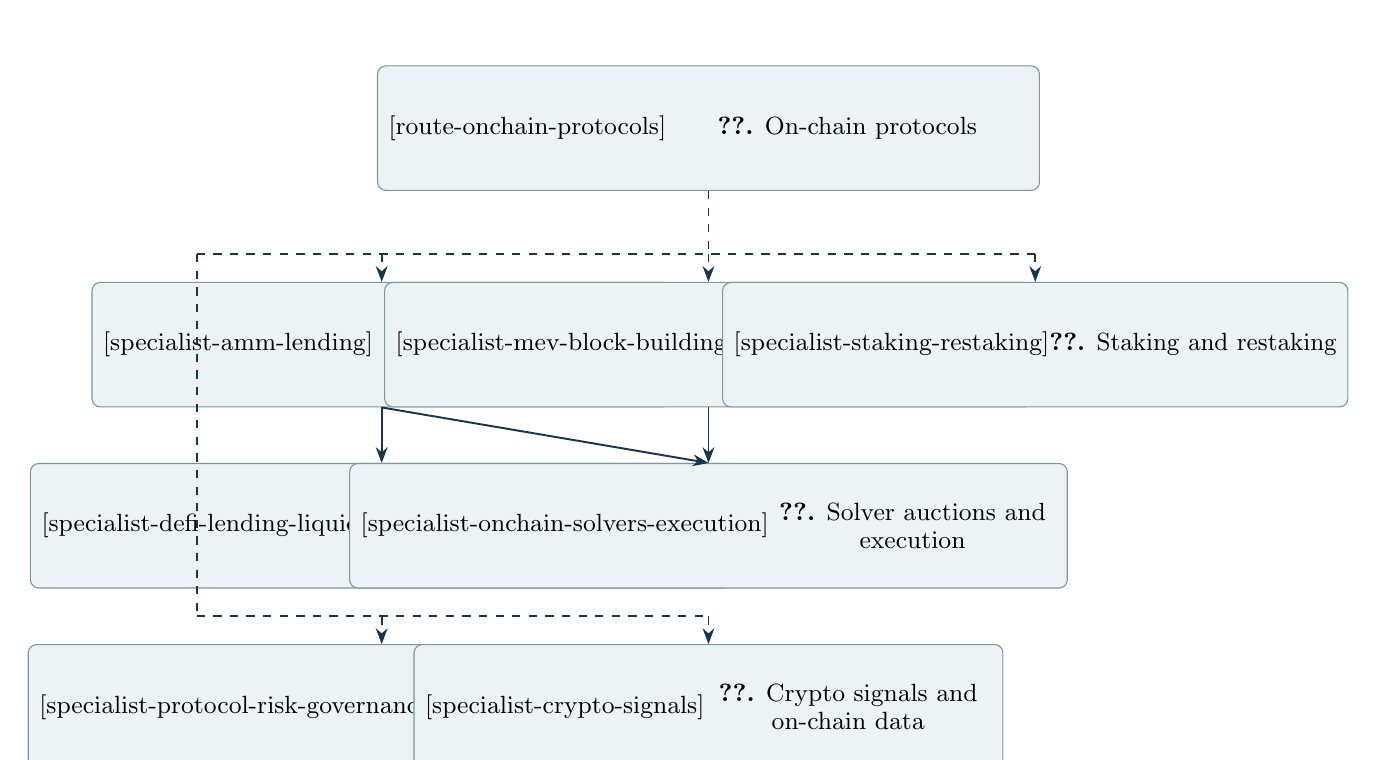
\begin{tikzpicture}[x=1cm,y=1cm]
\node[pathnode] (onchain-protocols) at (4.15,0) {\MeasurePathNode{4.6cm}{\textbf{\ref*{route-onchain-protocols}.} On-chain protocols}\hyperref[route-onchain-protocols]{\parbox[c][\pathnodeheight][c]{4.6cm}{\centering \textbf{\ref*{route-onchain-protocols}.} On-chain protocols}}};
\node[pathnode] (amm-lending) at (0.00,-2.75) {\MeasurePathNode{3.65cm}{\textbf{\ref*{specialist-amm-lending}.} AMMs and LP returns}\hyperref[specialist-amm-lending]{\parbox[c][\pathnodeheight][c]{3.65cm}{\centering \textbf{\ref*{specialist-amm-lending}.} AMMs and LP returns}}};
\node[pathnode] (mev-block-building) at (4.15,-2.75) {\MeasurePathNode{3.65cm}{\textbf{\ref*{specialist-mev-block-building}.} MEV and block building}\hyperref[specialist-mev-block-building]{\parbox[c][\pathnodeheight][c]{3.65cm}{\centering \textbf{\ref*{specialist-mev-block-building}.} MEV and block building}}};
\node[pathnode] (staking-restaking) at (8.30,-2.75) {\MeasurePathNode{3.65cm}{\textbf{\ref*{specialist-staking-restaking}.} Staking and restaking}\hyperref[specialist-staking-restaking]{\parbox[c][\pathnodeheight][c]{3.65cm}{\centering \textbf{\ref*{specialist-staking-restaking}.} Staking and restaking}}};
\node[pathnode] (defi-lending-liquidations) at (0.00,-5.05) {\MeasurePathNode{3.65cm}{\textbf{\ref*{specialist-defi-lending-liquidations}.} Lending and oracles}\hyperref[specialist-defi-lending-liquidations]{\parbox[c][\pathnodeheight][c]{3.65cm}{\centering \textbf{\ref*{specialist-defi-lending-liquidations}.} Lending and oracles}}};
\node[pathnode] (onchain-solvers-execution) at (4.15,-5.05) {\MeasurePathNode{3.65cm}{\textbf{\ref*{specialist-onchain-solvers-execution}.} Solver auctions and execution}\hyperref[specialist-onchain-solvers-execution]{\parbox[c][\pathnodeheight][c]{3.65cm}{\centering \textbf{\ref*{specialist-onchain-solvers-execution}.} Solver auctions and execution}}};
\node[pathnode] (protocol-risk-governance) at (0.00,-7.35) {\MeasurePathNode{3.65cm}{\textbf{\ref*{specialist-protocol-risk-governance}.} Exploits, bridges and DAOs}\hyperref[specialist-protocol-risk-governance]{\parbox[c][\pathnodeheight][c]{3.65cm}{\centering \textbf{\ref*{specialist-protocol-risk-governance}.} Exploits, bridges and DAOs}}};
\node[pathnode] (crypto-signals) at (4.15,-7.35) {\MeasurePathNode{3.65cm}{\textbf{\ref*{specialist-crypto-signals}.} Crypto signals and on-chain data}\hyperref[specialist-crypto-signals]{\parbox[c][\pathnodeheight][c]{3.65cm}{\centering \textbf{\ref*{specialist-crypto-signals}.} Crypto signals and on-chain data}}};
\draw[entryline] (onchain-protocols.south) -- (4.15,-1.60);
\draw[entryline] (-2.35,-1.60) -- (-2.35,-6.20);
\draw[entryline] (-2.35,-1.60) -- (8.30,-1.60);
\draw[entryarrow] (0.00,-1.60) -- (amm-lending.north);
\draw[entryarrow] (4.15,-1.60) -- (mev-block-building.north);
\draw[entryarrow] (8.30,-1.60) -- (staking-restaking.north);
\draw[entryline] (-2.35,-6.20) -- (4.15,-6.20);
\draw[entryarrow] (0.00,-6.20) -- (protocol-risk-governance.north);
\draw[entryarrow] (4.15,-6.20) -- (crypto-signals.north);
\draw[patharrow] (amm-lending.south) -- (defi-lending-liquidations.north);
\draw[patharrow] (amm-lending.south) -- (onchain-solvers-execution.north);
\draw[patharrow] (mev-block-building.south) -- (onchain-solvers-execution.north);
\end{tikzpicture}\end{center}
\textbf{Bring these foundations with you.}\begin{itemize}
\item \hyperref[route-execution-trading-costs]{Execution, trading costs and market structure} --- needed by \hyperref[specialist-onchain-solvers-execution]{Solver auctions and execution}.
\item \hyperref[route-common-toolkit]{Common toolkit} --- needed by \hyperref[specialist-crypto-signals]{Crypto signals and on-chain data}.
\item \hyperref[route-research-engineering-validation]{Research engineering and validation} --- needed by \hyperref[specialist-crypto-signals]{Crypto signals and on-chain data}.
\end{itemize}\hyperref[learning-map]{Return to the whole-guide DAG.}
\Needspace{12\baselineskip}
\subsection{Automated market makers: pricing, routing and liquidity-provider returns}\label{specialist-amm-lending}
\textbf{Specialist pathway.} In \hyperref[route-onchain-protocols]{On-chain protocols}.

\textbf{Outcome.} Price swaps and routes across constant-function and concentrated-liquidity pools, and decompose LP returns into inventory exposure, fees, arbitrage loss and rebalancing cost.

\textbf{Prerequisites.} On-chain protocols; smart-contract state and market making. Loss-versus-rebalancing from the overview is assumed.

\textbf{Review first.} \hyperref[route-onchain-protocols]{On-chain protocols}.

\textbf{Required readings, in order}
\begin{enumerate}\raggedright
\Needspace{5\baselineskip}\item \href{institutional_quantitative_finance_reading_list.pdf\#oc-xu-sok-dex-2023}{Jiahua Xu, Krzysztof Paruch, Simon Cousaert and Yebo Feng, ``SoK: Decentralized Exchanges (DEX) with Automated Market Maker (AMM) Protocols''}\CataloguePage{479}\NoteKey{oc-xu-sok-dex-2023}\par \textbf{Foundations.} Compare conservation, slippage and divergence-loss functions across the main AMM designs in one framework.
\Needspace{5\baselineskip}\item \href{institutional_quantitative_finance_reading_list.pdf\#s6-cfmm}{Guillermo Angeris and Tarun Chitra, ``Improved Price Oracles: Constant Function Market Makers''}\CataloguePage{445}\NoteKey{s6-cfmm}\par \textbf{Valuation.} Derive reserve invariants and marginal AMM prices.
\Needspace{5\baselineskip}\item \href{institutional_quantitative_finance_reading_list.pdf\#roadmap-cfmm-convex}{Guillermo Angeris, Akshay Agrawal, Alex Evans, Tarun Chitra, Stephen Boyd, Constant Function Market Makers: Multi-Asset Trades via Convex Optimization; Published handbook contents; Author manuscript}\CataloguePage{445}\NoteKey{roadmap-cfmm-convex}\par \textbf{Valuation.} Formulate admissible multi-asset trades as a convex problem before building a network route.
\Needspace{5\baselineskip}\item \href{institutional_quantitative_finance_reading_list.pdf\#roadmap-cfmm-routing}{Guillermo Angeris, Alex Evans, Tarun Chitra, Stephen Boyd, Optimal Routing for Constant Function Market Makers; Author manuscript and code; Preprint}\CataloguePage{445}\NoteKey{roadmap-cfmm-routing}\par \textbf{Optimization.} Choose route and size jointly; distinguish convex routing without fixed costs from mixed-integer pool activation.
\Needspace{5\baselineskip}\item \href{institutional_quantitative_finance_reading_list.pdf\#s6-uniswap}{Hayden Adams et al., ``Uniswap v3 Core''}\CataloguePage{445}\NoteKey{s6-uniswap}\par \textbf{Mechanics.} Map concentrated-liquidity positions and fee accrual.
\Needspace{5\baselineskip}\item \href{institutional_quantitative_finance_reading_list.pdf\#s11-r12}{Guillermo Angeris, Hsien-Tang Kao, Rei Chiang, Charlie Noyes and Tarun Chitra, \emph{An analysis of Uniswap markets} (2019 preprint); Uniswap v2 Core specification}\CataloguePage{477}\NoteKey{s11-r12}\par\emph{Selection:} Uniswap v2 Core companion and the 2019 analytical paper; distinct versions, one canonical entry.\par \textbf{Mechanics and evidence.} Read the v2 Core companion first for exact swaps and flash repayment, then the separately identified 2019 paper for arbitrage and price deviations.
\Needspace{5\baselineskip}\item \href{institutional_quantitative_finance_reading_list.pdf\#exp-uniswap4}{Hayden Adams et al., Uniswap v4 Core; core repository}\CataloguePage{478}\NoteKey{exp-uniswap4}\par \textbf{Mechanics.} Read hooks, dynamic fees and custom-accounting boundaries.
\Needspace{5\baselineskip}\item \href{institutional_quantitative_finance_reading_list.pdf\#roadmap-amm-fees}{Jason Milionis, Ciamac C. Moallemi, Tim Roughgarden, Automated Market Making and Arbitrage Profits in the Presence of Fees}\CataloguePage{478}\NoteKey{roadmap-amm-fees}\par \textbf{Valuation.} Add trading fees, block timing and fixed execution costs to the arbitrage/LP comparison.
\Needspace{5\baselineskip}\item \href{institutional_quantitative_finance_reading_list.pdf\#oc-hasbrouck-rivera-saleh-cl-2026}{Joel Hasbrouck, Thomas J. Rivera and Fahad Saleh, ``An Economic Model of a Decentralized Exchange with Concentrated Liquidity''}\CataloguePage{480}\NoteKey{oc-hasbrouck-rivera-saleh-cl-2026}\par \textbf{Theory.} Value a concentrated-liquidity position as a covered call sold at intrinsic value, and see why liquidity falls as the time premium rises.
\Needspace{5\baselineskip}\item \href{institutional_quantitative_finance_reading_list.pdf\#oc-hasbrouck-rivera-saleh-fees-2026}{Joel Hasbrouck, Thomas J. Rivera and Fahad Saleh, ``The Need for Fees at a DEX: How Increases in Fees Can Increase DEX Trading Volume''}\CataloguePage{480}\NoteKey{oc-hasbrouck-rivera-saleh-fees-2026}\par \textbf{Theory.} Explain why a higher fee tier can deepen a pool and lower the all-in cost of trading.
\Needspace{5\baselineskip}\item \href{institutional_quantitative_finance_reading_list.pdf\#oc-cartea-drissi-monga-2024}{Álvaro Cartea, Fayçal Drissi and Marcello Monga, ``Decentralized Finance and Automated Market Making: Predictable Loss and Optimal Liquidity Provision''}\CataloguePage{480}\NoteKey{oc-cartea-drissi-monga-2024}\par \textbf{Valuation.} Derive an LP's wealth dynamics and an optimal range width from fees net of gas, predictable loss and concentration risk.
\Needspace{5\baselineskip}\item \href{institutional_quantitative_finance_reading_list.pdf\#wide-lehar-parlour-uniswap}{Andreas Lehar and Christine A. Parlour, ``Decentralized Exchange: The Uniswap Automated Market Maker''}\CataloguePage{478}\NoteKey{wide-lehar-parlour-uniswap}\par \textbf{Evidence.} Compare the AMM with a limit order book in equilibrium and in the full record of Uniswap interactions.
\Needspace{5\baselineskip}\item \href{institutional_quantitative_finance_reading_list.pdf\#wide-capponi-jia-dex}{Agostino Capponi and Ruizhe Jia, ``Liquidity Provision on Blockchain-Based Decentralized Exchanges''}\CataloguePage{478}\NoteKey{wide-capponi-jia-dex}\par \textbf{Evidence.} See why LPs do not exit before arbitrage losses, where arbitrage rents go, and how LPs change pricing curves under stress.
\Needspace{5\baselineskip}\item \href{institutional_quantitative_finance_reading_list.pdf\#oc-heimbach-schertenleib-wattenhofer-2022}{Lioba Heimbach, Eric Schertenleib and Roger Wattenhofer, ``Risks and Returns of Uniswap V3 Liquidity Providers''}\CataloguePage{480}\NoteKey{oc-heimbach-schertenleib-wattenhofer-2022}\par \textbf{Evidence.} Measure how widely realised Uniswap v3 LP returns vary with range choice and active management.
\Needspace{5\baselineskip}\item \href{institutional_quantitative_finance_reading_list.pdf\#exp-amamm}{Austin Adams, Ciamac C. Moallemi, Sara Reynolds and Dan Robinson, am-AMM: An Auction-Managed Automated Market Maker; author proceedings record}\CataloguePage{478}\NoteKey{exp-amamm}\par \textbf{Evidence.} Examine auction-managed fee and arbitrage-value claims.
\Needspace{5\baselineskip}\item \href{institutional_quantitative_finance_reading_list.pdf\#s11-r11}{Dune documentation; The Graph subgraphs; Glassnode Studio (documentation)}\CataloguePage{476}\NoteKey{s11-r11}\par \textbf{Data.} Reconstruct pool state and event timing from chain queries.
\end{enumerate}
\Needspace{5\baselineskip}\textbf{Checkpoint.} Replay a chosen pool's deposits, swaps, fee accrual and withdrawals at pinned blocks; compare LP P\&L with hold and rebalanced benchmarks and with the predictable-loss measure, and attribute the difference to fees, arbitrage loss and range changes. Route one large swap across at least two pools with gas and delayed inclusion, then repeat after a fee-tier change and record which pool depth moved. Record contract addresses, versions, hook behaviour and any missing off-chain order flow.

\textbf{Optional branches.} \href{institutional_quantitative_finance_reading_list.pdf\#oc-mohan-2022}{Start with a geometric primer on AMM exchange functions.}\BranchPage{479} \href{institutional_quantitative_finance_reading_list.pdf\#roadmap-cfmm-routing-efficient}{Use the decomposition algorithm when the initial CFMM route optimizer becomes computationally limiting.}\BranchPage{445} \href{institutional_quantitative_finance_reading_list.pdf\#roadmap-dynamic-amm-fees}{Study dynamic fees after defining LP wealth and the comparison benchmark.}\BranchPage{478} \href{institutional_quantitative_finance_reading_list.pdf\#oc-cartea-drissi-monga-2023}{Compute predictable loss model-free and compare it with collected fees.}\BranchPage{480} \href{institutional_quantitative_finance_reading_list.pdf\#catalogue-0830}{Treat optimal liquidity provision as a mechanism-design problem with informed flow.}\BranchPage{444} \href{institutional_quantitative_finance_reading_list.pdf\#s6-fan}{Optimise concentrated-liquidity ranges dynamically against fees, out-of-range exposure and gas.}\BranchPage{445} \href{institutional_quantitative_finance_reading_list.pdf\#w3-aqsha-amm-lp-reward}{Model the reward contract between an AMM venue and strategic LPs.}\BranchPage{479} \href{institutional_quantitative_finance_reading_list.pdf\#oc-aoyagi-ito-2025}{Model liquidity spillovers between an AMM and a coexisting limit order book.}\BranchPage{480} \href{institutional_quantitative_finance_reading_list.pdf\#w3-dinosse-defi-stylized}{Compare stylised facts of concentrated-liquidity pools with order-book markets.}\BranchPage{440} \href{institutional_quantitative_finance_reading_list.pdf\#wide-park-amm-flaws}{Read a critique of constant-function market makers.}\BranchPage{478} \href{institutional_quantitative_finance_reading_list.pdf\#w3-capponi-jia-yu-dex-discovery}{See priority fees reveal informed DEX trades.}\BranchPage{478} \href{institutional_quantitative_finance_reading_list.pdf\#w3-schlegel-cfmm-axioms}{Characterise CFMMs axiomatically.}\BranchPage{479} \href{institutional_quantitative_finance_reading_list.pdf\#w4-echenim-gobet-uniswap}{Model Uniswap v3 impermanent loss and fees rigorously.}\BranchPage{479} \href{institutional_quantitative_finance_reading_list.pdf\#roadmap-foundry-anvil}{Verify swaps and revert paths on a reproducible fixed-block fork.}\BranchPage{529}
\par{\small \hyperref[learning-map]{Learning pathway DAG} \textbar{} \hyperref[route-onchain-protocols]{Section overview} \textbar{} \hyperref[map-onchain-protocols]{Section DAG}\NoteKey{amm-lending}}
\Needspace{12\baselineskip}
\subsection{Transaction ordering, MEV and block building}\label{specialist-mev-block-building}
\textbf{Specialist pathway.} In \hyperref[route-onchain-protocols]{On-chain protocols}.

\textbf{Outcome.} Measure who extracts value from transaction ordering, how private order flow and proposer-builder separation redistribute it, and what fee mechanisms and countermeasures can and cannot change.

\textbf{Prerequisites.} On-chain protocols; auction basics. Execution, trading costs and market structure (19) helps for the comparison with high-frequency trading.

\textbf{Review first.} \hyperref[route-onchain-protocols]{On-chain protocols}.

\textbf{Required readings, in order}
\begin{enumerate}\raggedright
\Needspace{5\baselineskip}\item \href{institutional_quantitative_finance_reading_list.pdf\#oc-torres-camino-state-2021}{Christof Ferreira Torres, Ramiro Camino and Radu State, ``Frontrunner Jones and the Raiders of the Dark Forest: An Empirical Study of Frontrunning on the Ethereum Blockchain''}\CataloguePage{441}\NoteKey{oc-torres-camino-state-2021}\par \textbf{Evidence.} Define displacement, insertion and suppression and measure front-running in the public mempool.
\Needspace{5\baselineskip}\item \href{institutional_quantitative_finance_reading_list.pdf\#oc-qin-zhou-gervais-2022}{Kaihua Qin, Liyi Zhou and Arthur Gervais, ``Quantifying Blockchain Extractable Value: How dark is the forest?''}\CataloguePage{441}\NoteKey{oc-qin-zhou-gervais-2022}\par \textbf{Evidence.} Quantify value extracted from sandwiches, liquidations and arbitrage, and see how relays affect consensus incentives.
\Needspace{5\baselineskip}\item \href{institutional_quantitative_finance_reading_list.pdf\#s6-auctiondocs}{Flashbots, \emph{Flashbots Auction: Overview and Documentation}}\CataloguePage{440}\NoteKey{s6-auctiondocs}\par \textbf{Mechanics.} Read how bundles, relays and MEV-Boost work and which trust assumptions private submission keeps.
\Needspace{5\baselineskip}\item \href{institutional_quantitative_finance_reading_list.pdf\#oc-weintraub-2022}{Ben Weintraub, Christof Ferreira Torres, Cristina Nita-Rotaru and Radu State, ``A Flash(bot) in the Pan: Measuring Maximal Extractable Value in Private Pools''}\CataloguePage{441}\NoteKey{oc-weintraub-2022}\par \textbf{Evidence.} Test whether a private pool removed MEV or moved it to the largest miners.
\Needspace{5\baselineskip}\item \href{institutional_quantitative_finance_reading_list.pdf\#w3-capponi-jia-wang-mev}{Agostino Capponi, Ruizhe Jia and Kanye Ye Wang, ``Maximal extractable value and allocative inefficiencies in public blockchains''}\CataloguePage{440}\NoteKey{w3-capponi-jia-wang-mev}\par \textbf{Theory.} Explain why private pools are adopted only partly when validators earn front-running rents.
\Needspace{5\baselineskip}\item \href{institutional_quantitative_finance_reading_list.pdf\#oc-heimbach-pbs-2023}{Lioba Heimbach, Lucianna Kiffer, Christof Ferreira Torres and Roger Wattenhofer, ``Ethereum's Proposer-Builder Separation: Promises and Realities''}\CataloguePage{441}\NoteKey{oc-heimbach-pbs-2023}\par \textbf{Evidence.} Measure builder and relay concentration, censorship and relay reliability under proposer-builder separation.
\Needspace{5\baselineskip}\item \href{institutional_quantitative_finance_reading_list.pdf\#oc-gupta-pai-resnick-2023}{Tivas Gupta, Mallesh M. Pai and Max Resnick, ``The Centralizing Effects of Private Order Flow on Proposer-Builder Separation''}\CataloguePage{441}\NoteKey{oc-gupta-pai-resnick-2023}\par \textbf{Theory.} See why private order flow favours builders integrated with searchers.
\Needspace{5\baselineskip}\item \href{institutional_quantitative_finance_reading_list.pdf\#oc-oz-2024}{Burak Öz, Danning Sui, Thomas Thiery and Florian Matthes, ``Who Wins Ethereum Block Building Auctions and Why?''}\CataloguePage{441}\NoteKey{oc-oz-2024}\par \textbf{Evidence.} Identify the order-flow features that win block auctions and the barrier they create for new builders.
\Needspace{5\baselineskip}\item \href{institutional_quantitative_finance_reading_list.pdf\#oc-roughgarden-tfm-2024}{Tim Roughgarden, ``Transaction Fee Mechanism Design''}\CataloguePage{442}\NoteKey{oc-roughgarden-tfm-2024}\par \textbf{Theory.} Analyse transaction fee mechanisms and EIP-1559's incentive properties.
\Needspace{5\baselineskip}\item \href{institutional_quantitative_finance_reading_list.pdf\#oc-liu-eip1559-2022}{Yulin Liu, Yuxuan Lu, Kartik Nayak, Fan Zhang, Luyao Zhang and Yinhong Zhao, ``Empirical Analysis of EIP-1559: Transaction Fees, Waiting Times, and Consensus Security''}\CataloguePage{442}\NoteKey{oc-liu-eip1559-2022}\par \textbf{Evidence.} Measure EIP-1559's effects on fees, waiting times and consensus security.
\Needspace{5\baselineskip}\item \href{institutional_quantitative_finance_reading_list.pdf\#oc-yang-sok-mev-2024}{Sen Yang, Fan Zhang, Ken Huang, Xi Chen, Youwei Yang and Feng Zhu, ``SoK: MEV Countermeasures''}\CataloguePage{442}\NoteKey{oc-yang-sok-mev-2024}\par \textbf{Mechanics.} Place each MEV countermeasure in a taxonomy and check which security problems it addresses.
\Needspace{5\baselineskip}\item \href{institutional_quantitative_finance_reading_list.pdf\#oc-torres-l2-mev-2024}{Christof Ferreira Torres, Albin Mamuti, Ben Weintraub, Cristina Nita-Rotaru and Shweta Shinde, ``Rolling in the Shadows: Analyzing the Extraction of MEV Across Layer-2 Rollups''}\CataloguePage{442}\NoteKey{oc-torres-l2-mev-2024}\par \textbf{Evidence.} Compare MEV on rollups without public mempools with Ethereum, including cross-layer sandwiches.
\end{enumerate}
\Needspace{5\baselineskip}\textbf{Checkpoint.} For one week of blocks, classify each block's builder, relay, bid and proposer payment, and tag sandwiches, back-runs, liquidations and CEX-DEX arbitrage. Estimate the share of value going to searchers, builders and proposers, and the share of blocks built from exclusive order flow. For one user swap, compare expected execution through the public mempool, a private RPC and an order-flow auction, and state which of these numbers depend on data you cannot observe.

\textbf{Optional branches.} \href{institutional_quantitative_finance_reading_list.pdf\#s6-wu}{Simulate MEV-Boost bidding with latency and relay connectivity.}\BranchPage{440} \href{institutional_quantitative_finance_reading_list.pdf\#oc-bahrani-garimidi-roughgarden-2025}{Model whether skill differences among block producers must centralise stake and whether PBS undoes it.}\BranchPage{441} \href{institutional_quantitative_finance_reading_list.pdf\#oc-ferreira-parkes-2023}{Study verifiable sequencing rules as an alternative to auctioning order.}\BranchPage{442} \href{institutional_quantitative_finance_reading_list.pdf\#catalogue-0951}{Use the Flashbots repositories and specifications for builder and relay details.}\BranchPage{529} \href{institutional_quantitative_finance_reading_list.pdf\#s4-flashbots}{Follow current Flashbots writing on block building and BuilderNet.}\BranchPage{551} \href{institutional_quantitative_finance_reading_list.pdf\#crypto-uncommon}{Read a searcher's own account of MEV practice.}\BranchPage{494}
\par{\small \hyperref[learning-map]{Learning pathway DAG} \textbar{} \hyperref[route-onchain-protocols]{Section overview} \textbar{} \hyperref[map-onchain-protocols]{Section DAG}\NoteKey{mev-block-building}}
\Needspace{12\baselineskip}
\subsection{Staking, liquid staking and restaking}\label{specialist-staking-restaking}
\textbf{Specialist pathway.} In \hyperref[route-onchain-protocols]{On-chain protocols}.

\textbf{Outcome.} Distinguish validator rewards, liquid-claim redemption and fixed/floating yield claims, including slashing, maturity and secondary-market basis.

\textbf{Prerequisites.} On-chain protocols; Ethereum proof of stake and smart-contract risk.

\textbf{Review first.} \hyperref[route-onchain-protocols]{On-chain protocols}.

\textbf{Required readings, in order}
\begin{enumerate}\raggedright
\Needspace{5\baselineskip}\item \href{institutional_quantitative_finance_reading_list.pdf\#crypto-narayanan}{Arvind Narayanan, Joseph Bonneau, Edward Felten, Andrew Miller and Steven Goldfeder, \emph{Bitcoin and Cryptocurrency Technologies} (Princeton University Press, 2016)}\CataloguePage{436}\NoteKey{crypto-narayanan}\par \textbf{Mechanics.} Review consensus and ownership before evaluating token claims.
\Needspace{5\baselineskip}\item \href{institutional_quantitative_finance_reading_list.pdf\#depth-cong-staking-2025}{Lin William Cong, Zhiheng He and Ke Tang, The Tokenomics of Staking}\CataloguePage{483}\NoteKey{depth-cong-staking-2025}\par \textbf{Valuation.} Treat staking rewards as endogenous token economics.
\Needspace{5\baselineskip}\item \href{institutional_quantitative_finance_reading_list.pdf\#depth-ethereum-staking-exits}{Ethereum Foundation, Staking Withdrawals; EIP-7002: Execution-Layer-Triggerable Withdrawals}\CataloguePage{483}\NoteKey{depth-ethereum-staking-exits}\par \textbf{Mechanics.} Map validator balance, exit queue and withdrawal credentials.
\Needspace{5\baselineskip}\item \href{institutional_quantitative_finance_reading_list.pdf\#depth-ethereum-slashing}{Ethereum Foundation, Proof-of-Stake Rewards and Penalties}\CataloguePage{483}\NoteKey{depth-ethereum-slashing}\par \textbf{Valuation.} Stress missed duties and correlated slash losses.
\Needspace{5\baselineskip}\item \href{institutional_quantitative_finance_reading_list.pdf\#depth-lido-liquid-staking}{Lido DAO, Lido Tokens Integration Guide; Accounting Oracle}\CataloguePage{483}\NoteKey{depth-lido-liquid-staking}\par \textbf{Mechanics.} Distinguish rebasing claims, wrapper tokens and withdrawal NFTs.
\Needspace{5\baselineskip}\item \href{institutional_quantitative_finance_reading_list.pdf\#depth-eigenlayer-restaking}{Eigen Labs, Slashing Goes Live on Mainnet; ELIP-002: Slashing}\CataloguePage{484}\NoteKey{depth-eigenlayer-restaking}\par \textbf{Mechanics.} Add service-specific slash and withdrawal rights.
\Needspace{5\baselineskip}\item \href{institutional_quantitative_finance_reading_list.pdf\#s11-r11}{Dune documentation; The Graph subgraphs; Glassnode Studio (documentation)}\CataloguePage{476}\NoteKey{s11-r11}\par \textbf{Data.} Observe dated balances, operators and queue events on-chain.
\Needspace{5\baselineskip}\item \href{institutional_quantitative_finance_reading_list.pdf\#s6-cryptofactors}{Yukun Liu, Aleh Tsyvinski and Xi Wu, ``Common Risk Factors in Cryptocurrency''; NBER working paper}\CataloguePage{442}\NoteKey{s6-cryptofactors}\par \textbf{Evidence.} Separate token-price exposure from apparent yield.
\Needspace{5\baselineskip}\item \href{institutional_quantitative_finance_reading_list.pdf\#roadmap-yieldspace}{Allan Niemerg, Dan Robinson and Lev Livnev, YieldSpace: An Automated Liquidity Provider for Fixed Yield Tokens}\CataloguePage{484}\NoteKey{roadmap-yieldspace}\par \textbf{Valuation.} Derive a time-to-maturity AMM for zero-coupon claims before comparing spot and rate-market liquidity.
\Needspace{5\baselineskip}\item \href{institutional_quantitative_finance_reading_list.pdf\#roadmap-pendle-v2}{Pendle contributors, Pendle V2: Yield Tokenization, AMM and Order Book; Pendle V2 order book; Standardized Yield contracts}\CataloguePage{483}\NoteKey{roadmap-pendle-v2}\par \textbf{Mechanics.} Trace SY/PT/YT units, accrued yield and maturity redemption; separate fixed accounting-asset yield from dollar certainty.
\Needspace{5\baselineskip}\item \href{institutional_quantitative_finance_reading_list.pdf\#w3-john-pow-pos}{Kose John, Thomas J. Rivera and Fahad Saleh, ``Proof-of-Work versus Proof-of-Stake: A Comparative Economic Analysis''}\CataloguePage{484}\NoteKey{w3-john-pow-pos}\par \textbf{Theory.} Compare the equilibrium security of proof-of-stake and proof-of-work under realistic parameters.
\Needspace{5\baselineskip}\item \href{institutional_quantitative_finance_reading_list.pdf\#oc-grandjean-heimbach-wattenhofer-2024}{Dominic Grandjean, Lioba Heimbach and Roger Wattenhofer, ``Ethereum Proof-of-Stake Consensus Layer: Participation and Decentralization''}\CataloguePage{485}\NoteKey{oc-grandjean-heimbach-wattenhofer-2024}\par \textbf{Evidence.} Trace participation dips to clients, upgrades and large operators, and measure staking concentration.
\Needspace{5\baselineskip}\item \href{institutional_quantitative_finance_reading_list.pdf\#oc-scharnowski-jahanshahloo-2024}{Stefan Scharnowski and Hossein Jahanshahloo, ``The Economics of Liquid Staking Derivatives: Basis Determinants and Price Discovery''}\CataloguePage{485}\NoteKey{oc-scharnowski-jahanshahloo-2024}\par \textbf{Evidence.} Explain the liquid staking basis with yields, volatility, liquidity and sentiment.
\Needspace{5\baselineskip}\item \href{institutional_quantitative_finance_reading_list.pdf\#oc-durvasula-roughgarden-2025}{Naveen Durvasula and Tim Roughgarden, ``Robust Restaking Networks''}\CataloguePage{485}\NoteKey{oc-durvasula-roughgarden-2025}\par \textbf{Theory.} Bound cascading stake losses when validators secure several services.
\end{enumerate}
\Needspace{5\baselineskip}\textbf{Checkpoint.} Build an ETH-denominated cash-flow tree for native staking, stETH/wstETH and one restaked claim. Record effective balance, fee split, exit wait, market discount, oracle and slash event; value each under normal and correlated-loss scenarios at a pinned block and contract version. Extend the ledger to one dated PT/YT market: identify the redemption accounting asset, maturity cash flows, funding path, accrued yield and incentives separately; stress withdrawal delay and underlying redemption failure. Bound the restaked position's worst-case loss with the attack-cost buffer and compare the liquid staking basis on the pinned date with its drivers.

\textbf{Optional branches.} \href{institutional_quantitative_finance_reading_list.pdf\#w6-saleh-pos}{Read the economic case for proof-of-stake.}\BranchPage{484} \href{institutional_quantitative_finance_reading_list.pdf\#w6-cong-li-wang-platform}{Model token-financed platforms.}\BranchPage{484} \href{institutional_quantitative_finance_reading_list.pdf\#oc-gogol-lst-2024}{Compare LST protocol designs and the emerging restaking risks.}\BranchPage{484} \href{institutional_quantitative_finance_reading_list.pdf\#oc-xiong-wang-wang-2024}{Measure primary-secondary LST price gaps and LP returns in LST pools.}\BranchPage{485} \href{institutional_quantitative_finance_reading_list.pdf\#oc-schwarz-schilling-2022}{Study reorganisation attacks on proof-of-stake Ethereum and why finality matters.}\BranchPage{485}
\par{\small \hyperref[learning-map]{Learning pathway DAG} \textbar{} \hyperref[route-onchain-protocols]{Section overview} \textbar{} \hyperref[map-onchain-protocols]{Section DAG}\NoteKey{staking-restaking}}
\Needspace{12\baselineskip}
\subsection{DeFi lending, liquidations and price oracles}\label{specialist-defi-lending-liquidations}
\textbf{Specialist pathway.} In \hyperref[route-onchain-protocols]{On-chain protocols}.

\textbf{Outcome.} Model a lending pool's rate curve, leverage and liquidation path, price liquidation proceeds net of execution costs, and stress the oracle that triggers them.

\textbf{Prerequisites.} On-chain protocols; Automated market makers (32.1) for DEX resale slippage and pool-based price oracles. The chain-query tools from 32.1 are reused here.

\textbf{Review first.} \hyperref[route-onchain-protocols]{On-chain protocols}; \hyperref[specialist-amm-lending]{Automated market makers: pricing, routing and liquidity-provider returns}.

\textbf{Required readings, in order}
\begin{enumerate}\raggedright
\Needspace{5\baselineskip}\item \href{institutional_quantitative_finance_reading_list.pdf\#oc-chiu-kahn-koeppl-2022}{Jonathan Chiu, Charles M. Kahn and Thorsten V. Koeppl, ``Grasping decentralized finance through the lens of economic theory''}\CataloguePage{438}\NoteKey{oc-chiu-kahn-koeppl-2022}\par \textbf{Theory.} Set out what collateralised DeFi lending can gain over intermediated lending and where volatile collateral, incomplete contracts and oracles limit it.
\Needspace{5\baselineskip}\item \href{institutional_quantitative_finance_reading_list.pdf\#s11-r13}{Maker Team, \emph{The Dai Stablecoin System} (historical 2017 whitepaper); Compound Finance documentation (Comet specification)}\CataloguePage{480}\NoteKey{s11-r13}\par \textbf{Mechanics.} Define collateral, utilisation and liquidation in lending protocols.
\Needspace{5\baselineskip}\item \href{institutional_quantitative_finance_reading_list.pdf\#oc-gudgeon-plf-2020}{Lewis Gudgeon, Sam Werner, Daniel Perez and William J. Knottenbelt, ``DeFi Protocols for Loanable Funds: Interest Rates, Liquidity and Market Efficiency''}\CataloguePage{481}\NoteKey{oc-gudgeon-plf-2020}\par \textbf{Mechanics.} Compare utilisation-based rate rules on Compound, Aave and dYdX and test how rates co-move across protocols.
\Needspace{5\baselineskip}\item \href{institutional_quantitative_finance_reading_list.pdf\#w3-bertucci-defi-irm}{Charles Bertucci, Louis Bertucci, Mathis Gontier Delaunay, Olivier Guéant and Matthieu Lesbre, ``Agents' Behavior and Interest Rate Model Optimization in DeFi Lending''}\CataloguePage{481}\NoteKey{w3-bertucci-defi-irm}\par \textbf{Valuation.} Derive an optimal interest-rate model and compare it with controller-based rate policies.
\Needspace{5\baselineskip}\item \href{institutional_quantitative_finance_reading_list.pdf\#al-aave}{Emilio Frangella and Lasse Herskind, \emph{Aave V3 Technical Paper}; Aave Interest Rate Strategy documentation; Aave V3 Pool contract interface}\CataloguePage{184}\NoteKey{al-aave}\par \textbf{Implementation.} Check live protocol parameters and lifecycle for a specific lending pool.
\Needspace{5\baselineskip}\item \href{institutional_quantitative_finance_reading_list.pdf\#oc-perez-knife-edge-2021}{Daniel Perez, Sam M. Werner, Jiahua Xu and Benjamin Livshits, ``Liquidations: DeFi on a Knife-Edge''}\CataloguePage{481}\NoteKey{oc-perez-knife-edge-2021}\par \textbf{Evidence.} Measure how small price moves create large liquidatable volumes and how fast liquidators act.
\Needspace{5\baselineskip}\item \href{institutional_quantitative_finance_reading_list.pdf\#roadmap-defi-liquidations}{Kaihua Qin, Liyi Zhou, Pablo Gamito, Philipp Jovanovic and Arthur Gervais, An Empirical Study of DeFi Liquidations: Incentives, Risks, and Instabilities; Author preprint, arXiv v2; UCL accepted manuscript}\CataloguePage{481}\NoteKey{roadmap-defi-liquidations}\par \textbf{Evidence.} Reconstruct historical liquidations with contemporaneous eligibility, collateral proceeds and execution costs.
\Needspace{5\baselineskip}\item \href{institutional_quantitative_finance_reading_list.pdf\#oc-lehar-parlour-2022}{Alfred Lehar and Christine A. Parlour, ``Systemic fragility in decentralised markets''}\CataloguePage{482}\NoteKey{oc-lehar-parlour-2022}\par \textbf{Evidence.} Measure the DEX price impact of collateral sales by flash-loan liquidators and the feedback it creates.
\Needspace{5\baselineskip}\item \href{institutional_quantitative_finance_reading_list.pdf\#oc-klages-mundt-minca-2021}{Ariah Klages-Mundt and Andreea Minca, ``(In)Stability for the Blockchain: Deleveraging Spirals and Stablecoin Attacks''}\CataloguePage{482}\NoteKey{oc-klages-mundt-minca-2021}\par \textbf{Theory.} Model deleveraging spirals in crypto-collateralised stablecoins and the Black Thursday auction failure.
\Needspace{5\baselineskip}\item \href{institutional_quantitative_finance_reading_list.pdf\#oc-heimbach-huang-2024}{Lioba Heimbach and Wenqian Huang, ``DeFi leverage''}\CataloguePage{482}\NoteKey{oc-heimbach-huang-2024}\par \textbf{Evidence.} Measure wallet-level leverage and how it shifts debt toward the liquidation threshold.
\Needspace{5\baselineskip}\item \href{institutional_quantitative_finance_reading_list.pdf\#oc-chiu-danisman-2026}{Jonathan Chiu and Furkan Berk Danışman, ``DeFi Lending: Returns, Leverage, and Liquidation Risk''}\CataloguePage{482}\NoteKey{oc-chiu-danisman-2026}\par \textbf{Evidence.} Read a recent Aave V3 study of protocol revenue, recursive leverage and liquidation waves.
\Needspace{5\baselineskip}\item \href{institutional_quantitative_finance_reading_list.pdf\#oc-eskandari-oracles-2021}{Shayan Eskandari, Mehdi Salehi, Wanyun Catherine Gu and Jeremy Clark, ``SoK: Oracles from the Ground Truth to Market Manipulation''}\CataloguePage{482}\NoteKey{oc-eskandari-oracles-2021}\par \textbf{Mechanics.} Name the oracle design behind each price a lending market uses and its attack surface.
\Needspace{5\baselineskip}\item \href{institutional_quantitative_finance_reading_list.pdf\#oc-mackinga-twap-2022}{Torgin Mackinga, Tejaswi Nadahalli and Roger Wattenhofer, ``TWAP Oracle Attacks: Easier Done than Said?''}\CataloguePage{482}\NoteKey{oc-mackinga-twap-2022}\par \textbf{Counter-evidence.} Check whether a time-weighted average price oracle is as costly to manipulate as assumed, including by a proposer with consecutive blocks.
\end{enumerate}
\Needspace{5\baselineskip}\textbf{Checkpoint.} For one borrowing account on a pinned block, reconstruct the rate-model state, debt index, collateral, wallet leverage, oracle publication and maximum repay amount. Calculate liquidation proceeds net of gas, auction or fixed bonus and DEX resale slippage, including a lost-auction case and a flash-loan-funded liquidation. Stress the oracle with a stale update, a single-block TWAP manipulation and a 20\% collateral gap, and report how much debt becomes liquidatable and who bears any shortfall.

\textbf{Optional branches.} \href{institutional_quantitative_finance_reading_list.pdf\#roadmap-morpho-blue}{Compare isolated Morpho markets with pooled lending, including market-specific oracle, LLTV and rate-model identities.}\BranchPage{481} \href{institutional_quantitative_finance_reading_list.pdf\#roadmap-chainlink-svr}{Account for oracle-update auctions that can redistribute the liquidator's gross bonus.}\BranchPage{481} \href{institutional_quantitative_finance_reading_list.pdf\#oc-saengchote-2023}{See who borrows on Compound, for how long and for which yield-farming strategies.}\BranchPage{482} \href{institutional_quantitative_finance_reading_list.pdf\#oc-deng-oracle-2024}{Find contract parameters that stay safe under skewed oracle inputs.}\BranchPage{482} \href{institutional_quantitative_finance_reading_list.pdf\#oc-caldarelli-ellul-2021}{Read a non-technical review of the oracle problem and its hacks.}\BranchPage{483} \href{institutional_quantitative_finance_reading_list.pdf\#s4-gauntlet}{Compare practitioner simulation-based risk modelling for lending parameters.}\BranchPage{551} \href{institutional_quantitative_finance_reading_list.pdf\#roadmap-foundry-anvil}{Verify liquidation and revert paths on a reproducible fixed-block fork.}\BranchPage{529}
\par{\small \hyperref[learning-map]{Learning pathway DAG} \textbar{} \hyperref[route-onchain-protocols]{Section overview} \textbar{} \hyperref[map-onchain-protocols]{Section DAG}\NoteKey{defi-lending-liquidations}}
\Needspace{12\baselineskip}
\subsection{On-chain solver auctions and cross-domain execution}\label{specialist-onchain-solvers-execution}
\textbf{Specialist pathway.} In \hyperref[route-onchain-protocols]{On-chain protocols}.

\textbf{Outcome.} Price a signed-order or cross-domain opportunity after route feasibility, auction rules, ordering cost, failed legs and capital restoration.

\textbf{Prerequisites.} Execution, trading costs and market structure; On-chain protocols; Automated market makers (32.1) for exact swap arithmetic and CFMM route-and-size optimisation; Transaction ordering, MEV and block building (32.2) for private order flow and builder auctions; transaction lifecycle, finality and inventory finance.

\textbf{Review first.} \hyperref[route-execution-trading-costs]{Execution, trading costs and market structure}; \hyperref[route-onchain-protocols]{On-chain protocols}; \hyperref[specialist-amm-lending]{Automated market makers: pricing, routing and liquidity-provider returns}; \hyperref[specialist-mev-block-building]{Transaction ordering, MEV and block building}.

\textbf{Required readings, in order}
\begin{enumerate}\raggedright
\Needspace{5\baselineskip}\item \href{institutional_quantitative_finance_reading_list.pdf\#s6-mevscaling}{Robert Miller / Flashbots, ``MEV and the Limits of Scaling''}\CataloguePage{439}\NoteKey{s6-mevscaling}\par \textbf{Mechanics.} Frame ordering competition and private flow as economic constraints on accessible execution.
\Needspace{5\baselineskip}\item \href{institutional_quantitative_finance_reading_list.pdf\#roadmap-cex-dex-extracted}{Fei Wu, Danning Sui, Thomas Thiery and Mallesh Pai, Measuring CEX-DEX Extracted Value and Searcher Profitability: The Darkest of the MEV Dark Forest; Full arXiv version}\CataloguePage{439}\NoteKey{roadmap-cex-dex-extracted}\par \textbf{Evidence.} Separate estimated CEX-DEX extracted value from unobserved external hedges and net profits.
\Needspace{5\baselineskip}\item \href{institutional_quantitative_finance_reading_list.pdf\#roadmap-non-atomic-arbitrage}{Lioba Heimbach, Vabuk Pahari and Eric Schertenleib, Non-Atomic Arbitrage in Decentralized Finance; Author preprint, arXiv v3; Author replication repository}\CataloguePage{439}\NoteKey{roadmap-non-atomic-arbitrage}\par \textbf{Evidence.} Identify non-atomic arbitrage while retaining external-leg and inventory-restoration uncertainty.
\Needspace{5\baselineskip}\item \href{institutional_quantitative_finance_reading_list.pdf\#roadmap-cow-solvers}{CoW Protocol contributors, CoW Protocol: Solver Engine and Solver Competition Rules; Competition rules}\CataloguePage{440}\NoteKey{roadmap-cow-solvers}\par \textbf{Mechanics.} Convert signed orders into feasible routes, user limits, competition scores and solver cash flows.
\Needspace{5\baselineskip}\item \href{institutional_quantitative_finance_reading_list.pdf\#roadmap-uniswapx}{Uniswap Labs contributors, UniswapX Overview}\CataloguePage{440}\NoteKey{roadmap-uniswapx}\par \textbf{Mechanics.} Compare a second filling architecture; apply its chain-specific auction timing and output constraints.
\Needspace{5\baselineskip}\item \href{institutional_quantitative_finance_reading_list.pdf\#catalogue-0832}{Mengqian Zhang, Sen Yang and Fan Zhang, ``RediSwap: MEV Redistribution Mechanism for CFMMs''; preprint; evaluation code/data}\CataloguePage{444}\NoteKey{catalogue-0832}\par \textbf{Evidence.} Challenge theoretical MEV redistribution with gas, route, concentration and manipulation costs.
\Needspace{5\baselineskip}\item \href{institutional_quantitative_finance_reading_list.pdf\#roadmap-foundry-anvil}{Foundry contributors, Foundry: Anvil, forking and transaction tracing}\CataloguePage{529}\NoteKey{roadmap-foundry-anvil}\par \textbf{Implementation.} Verify one settlement route and failed route against pinned EVM state before attributing a simulated execution edge.
\end{enumerate}
\Needspace{5\baselineskip}\textbf{Checkpoint.} For one recorded or explicitly synthetic signed-order auction, preserve the request, user limit, local receipt, deadline, route state and simulated output. Reconcile submitted bid, acceptance, settlement trace, gas, tip, pool execution, external hedge and final inventory in one opportunity-to-outcome ledger. Add a failed bid, lost on-chain leg, delayed cross-domain hedge and eventual capital rebalance; distinguish submission acknowledgement, preconfirmation, inclusion and finality. Report a hypothetical solver edge only where request/response and access data are absent.

\textbf{Optional branches.} \href{institutional_quantitative_finance_reading_list.pdf\#catalogue-0831}{Compare encrypted and pre-decryption liquidity designs as a mechanism alternative.}\BranchPage{444} \href{institutional_quantitative_finance_reading_list.pdf\#section.18.10}{Inspect chain and exchange feed choices before synchronising states.}\BranchPage{493} \href{institutional_quantitative_finance_reading_list.pdf\#roadmap-chainlink-svr}{Study oracle-triggered liquidation backrun auctions as a separate execution-access constraint.}\BranchPage{481} \href{institutional_quantitative_finance_reading_list.pdf\#w4-baude-challet-uniswap-execution}{Liquidate optimally on Uniswap v2/v3.}\BranchPage{479} \href{institutional_quantitative_finance_reading_list.pdf\#w4-alexander-uniswap-discovery}{Compare DEX and CEX price discovery.}\BranchPage{479}
\par{\small \hyperref[learning-map]{Learning pathway DAG} \textbar{} \hyperref[route-onchain-protocols]{Section overview} \textbar{} \hyperref[map-onchain-protocols]{Section DAG}\NoteKey{onchain-solvers-execution}}
\Needspace{12\baselineskip}
\subsection{Protocol risk and governance: exploits, bridges, layer two and DAOs}\label{specialist-protocol-risk-governance}
\textbf{Specialist pathway.} In \hyperref[route-onchain-protocols]{On-chain protocols}.

\textbf{Outcome.} Classify a protocol's exposure to contract bugs, economic exploits, bridge and rollup failure and governance capture, and judge what audits, tools and voting rules actually reduce.

\textbf{Prerequisites.} On-chain protocols; smart-contract state and transaction tracing. DeFi lending, liquidations and price oracles (32.4) helps for flash-loan and oracle attacks.

\textbf{Review first.} \hyperref[route-onchain-protocols]{On-chain protocols}.

\textbf{Required readings, in order}
\begin{enumerate}\raggedright
\Needspace{5\baselineskip}\item \href{institutional_quantitative_finance_reading_list.pdf\#oc-atzei-2017}{Nicola Atzei, Massimo Bartoletti and Tiziana Cimoli, ``A Survey of Attacks on Ethereum Smart Contracts (SoK)''}\CataloguePage{494}\NoteKey{oc-atzei-2017}\par \textbf{Foundations.} Learn the common smart-contract programming pitfalls and the attacks that exploit them.
\Needspace{5\baselineskip}\item \href{institutional_quantitative_finance_reading_list.pdf\#w2-qin-flash-loans}{Kaihua Qin, Liyi Zhou, Benjamin Livshits and Arthur Gervais, ``Attacking the DeFi Ecosystem with Flash Loans for Fun and Profit''}\CataloguePage{494}\NoteKey{w2-qin-flash-loans}\par \textbf{Evidence.} See how atomic flash loans finance attacks and how attack parameters are optimised.
\Needspace{5\baselineskip}\item \href{institutional_quantitative_finance_reading_list.pdf\#oc-chaliasos-2024}{Stefanos Chaliasos, Marcos Antonios Charalambous, Liyi Zhou, Rafaila Galanopoulou, Arthur Gervais, Dimitris Mitropoulos and Benjamin Livshits, ``Smart Contract and DeFi Security Tools: Do They Meet the Needs of Practitioners?''}\CataloguePage{494}\NoteKey{oc-chaliasos-2024}\par \textbf{Counter-evidence.} Check how few historical exploits automated security tools would have caught.
\Needspace{5\baselineskip}\item \href{institutional_quantitative_finance_reading_list.pdf\#s11-r23}{Olympix, ``A Comprehensive Analysis of Smart Contract Security Approaches: Auditing, Mutation Testing, Formal Verification, and Fuzzing'' (source: 2024)}\CataloguePage{493}\NoteKey{s11-r23}\par \textbf{Methods.} Compare audits, mutation testing, fuzzing and formal verification and what each proves.
\Needspace{5\baselineskip}\item \href{institutional_quantitative_finance_reading_list.pdf\#oc-zamyatin-2021}{Alexei Zamyatin, Mustafa Al-Bassam, Dionysis Zindros, Eleftherios Kokoris-Kogias, Pedro Moreno-Sanchez, Aggelos Kiayias and William J. Knottenbelt, ``SoK: Communication Across Distributed Ledgers''}\CataloguePage{495}\NoteKey{oc-zamyatin-2021}\par \textbf{Theory.} Understand why cross-chain communication needs a trusted party and how to evaluate a bridge's trust model.
\Needspace{5\baselineskip}\item \href{institutional_quantitative_finance_reading_list.pdf\#oc-zhang-bridges-2024}{Mengya Zhang, Xiaokuan Zhang, Yinqian Zhang and Zhiqiang Lin, ``Security of Cross-chain Bridges: Attack Surfaces, Defenses, and Open Problems''}\CataloguePage{495}\NoteKey{oc-zhang-bridges-2024}\par \textbf{Evidence.} Classify bridge attacks and their defences.
\Needspace{5\baselineskip}\item \href{institutional_quantitative_finance_reading_list.pdf\#oc-notland-2026}{Jakob Svennevik Notland, Jingyue Li, Mariusz Nowostawski and Peter Halland Haro, ``SoK: cross-chain bridging architectural design flaws and mitigations''}\CataloguePage{495}\NoteKey{oc-notland-2026}\par \textbf{Evidence.} Link bridge architecture components to design flaws and past exploits.
\Needspace{5\baselineskip}\item \href{institutional_quantitative_finance_reading_list.pdf\#oc-gudgeon-sok-l2-2020}{Lewis Gudgeon, Pedro Moreno-Sanchez, Stefanie Roos, Patrick McCorry and Arthur Gervais, ``SoK: Layer-Two Blockchain Protocols''}\CataloguePage{495}\NoteKey{oc-gudgeon-sok-l2-2020}\par \textbf{Mechanics.} Map channels, commit-chains and refereed delegation, and when layer-two balances are final.
\Needspace{5\baselineskip}\item \href{institutional_quantitative_finance_reading_list.pdf\#oc-fritsch-muller-wattenhofer-2024}{Robin Fritsch, Marino Müller and Roger Wattenhofer, ``Analyzing voting power in decentralized governance: Who controls DAOs?''}\CataloguePage{495}\NoteKey{oc-fritsch-muller-wattenhofer-2024}\par \textbf{Evidence.} Measure how concentrated DAO voting power is and how it is used.
\Needspace{5\baselineskip}\item \href{institutional_quantitative_finance_reading_list.pdf\#oc-barbereau-2023}{Tom Barbereau, Reilly Smethurst, Orestis Papageorgiou, Johannes Sedlmeir and Gilbert Fridgen, ``Decentralised Finance’s timocratic governance: The distribution and exercise of tokenised voting rights''}\CataloguePage{495}\NoteKey{oc-barbereau-2023}\par \textbf{Evidence.} See how concentrated and little used governance-token voting rights are across major DeFi projects.
\Needspace{5\baselineskip}\item \href{institutional_quantitative_finance_reading_list.pdf\#oc-han-lee-li-2026}{Jungsuk Han, Jongsub Lee and Tao Li, ``Decentralized Autonomous Organization Governance''}\CataloguePage{496}\NoteKey{oc-han-lee-li-2026}\par \textbf{Theory.} Model the conflict between a large token holder and small holders and its effect on platform growth.
\Needspace{5\baselineskip}\item \href{institutional_quantitative_finance_reading_list.pdf\#oc-fsb-defi-2023}{Financial Stability Board, The Financial Stability Risks of Decentralised Finance}\CataloguePage{438}\NoteKey{oc-fsb-defi-2023}\par \textbf{Regulation.} Read the FSB's account of operational, liquidity, leverage and interconnection vulnerabilities and the monitoring data it asks for.
\end{enumerate}
\Needspace{5\baselineskip}\textbf{Checkpoint.} For one live protocol on a pinned date, list its admin keys, upgrade path and timelock, oracle and bridge dependencies, and audit history. Measure the share of voting power held by the top ten holders and delegates and compare it with quorum. Replay one historical exploit of a similar protocol on a fixed-block fork, classify it by layer and state whether the cited tools or audits would have caught it. Estimate the loss if the main bridge or rollup failed, and state which risks the FSB and IOSCO frameworks would assign to an identifiable person.

\textbf{Optional branches.} \href{institutional_quantitative_finance_reading_list.pdf\#oc-thibault-2022}{Compare optimistic and zero-knowledge rollup designs and their performance.}\BranchPage{495} \href{institutional_quantitative_finance_reading_list.pdf\#oc-han-lee-li-review-2025}{Read a review of DAO governance and the whale problem.}\BranchPage{496} \href{institutional_quantitative_finance_reading_list.pdf\#oc-cong-harvey-rabetti-wu-2025}{See how crypto-enabled crime is organised and traced on-chain.}\BranchPage{495} \href{institutional_quantitative_finance_reading_list.pdf\#oc-aramonte-huang-schrimpf-2021}{Read the BIS case that DeFi governance is less decentralised than claimed.}\BranchPage{438} \href{institutional_quantitative_finance_reading_list.pdf\#crypto-defisafety}{Use published process-quality criteria for code, audits, admin controls and oracles.}\BranchPage{493} \href{institutional_quantitative_finance_reading_list.pdf\#s11-r25}{Practise exploitation and auditing on security exercises.}\BranchPage{493} \href{institutional_quantitative_finance_reading_list.pdf\#roadmap-foundry-anvil}{Replay exploits on a reproducible fixed-block fork.}\BranchPage{529}
\par{\small \hyperref[learning-map]{Learning pathway DAG} \textbar{} \hyperref[route-onchain-protocols]{Section overview} \textbar{} \hyperref[map-onchain-protocols]{Section DAG}\NoteKey{protocol-risk-governance}}
\Needspace{12\baselineskip}
\subsection{Crypto signals and on-chain evidence}\label{specialist-crypto-signals}
\textbf{Specialist pathway.} In \hyperref[route-onchain-protocols]{On-chain protocols}.

\textbf{Outcome.} Separate a causal crypto forecast from market-factor exposure, hindsight wallet labels, token-unit changes and untradeable gross returns.

\textbf{Prerequisites.} Common toolkit, On-chain protocols, and the Research engineering and validation treatment of known-at times; return accounting, token units and chronological validation. Crypto return dynamics (31.6) gives the time-series baseline and Crypto exchange market quality (31.2) the volume and manipulation screens. Cross-sectional crypto strategies (35.1) gives the factor and anomaly baseline.

\textbf{Review first.} \hyperref[route-onchain-protocols]{On-chain protocols}; \hyperref[route-common-toolkit]{Common toolkit}; \hyperref[route-research-engineering-validation]{Research engineering and validation}.

\textbf{Required readings, in order}
\begin{enumerate}\raggedright
\Needspace{5\baselineskip}\item \href{institutional_quantitative_finance_reading_list.pdf\#roadmap-crypto-risks-returns}{Yukun Liu and Aleh Tsyvinski, Risks and Returns of Cryptocurrency; NBER working paper 24877}\CataloguePage{442}\NoteKey{roadmap-crypto-risks-returns}\par \textbf{Evidence.} Reproduce crypto-specific return/attention hypotheses before testing incremental signals against the factor benchmark.
\Needspace{5\baselineskip}\item \href{institutional_quantitative_finance_reading_list.pdf\#s6-cryptofactors}{Yukun Liu, Aleh Tsyvinski and Xi Wu, ``Common Risk Factors in Cryptocurrency''; NBER working paper}\CataloguePage{442}\NoteKey{s6-cryptofactors}\par \textbf{Evidence.} Use market, size and momentum as the baseline before claiming a novel token signal.
\Needspace{5\baselineskip}\item \href{institutional_quantitative_finance_reading_list.pdf\#oc-bhambhwani-2023}{Siddharth M. Bhambhwani, Stefanos Delikouras and George M. Korniotis, ``Blockchain characteristics and cryptocurrency returns''}\CataloguePage{444}\NoteKey{oc-bhambhwani-2023}\par \textbf{Evidence.} Test network-size and computing-power factors against the return-based baseline.
\Needspace{5\baselineskip}\item \href{institutional_quantitative_finance_reading_list.pdf\#roadmap-bitcoin-entities}{Igor Makarov and Antoinette Schoar, Blockchain Analysis of the Bitcoin Market}\CataloguePage{475}\NoteKey{roadmap-bitcoin-entities}\par \textbf{Measurement.} Separate address-to-entity inference and retrospective labels from the information available at each forecast time.
\Needspace{5\baselineskip}\item \href{institutional_quantitative_finance_reading_list.pdf\#roadmap-blocksci}{Harry Kalodner, Malte Möser, Kevin Lee, Steven Goldfeder, Martin Plattner, Alishah Chator and Arvind Narayanan, BlockSci: Design and applications of a blockchain analysis platform; Proceedings paper}\CataloguePage{475}\NoteKey{roadmap-blocksci}\par \textbf{Data.} Inspect UTXO parsing and clustering heuristics; the selected BlockSci paper excludes Ethereum.
\Needspace{5\baselineskip}\item \href{institutional_quantitative_finance_reading_list.pdf\#s11-r11}{Dune documentation; The Graph subgraphs; Glassnode Studio (documentation)}\CataloguePage{476}\NoteKey{s11-r11}\par \textbf{Data.} Reconstruct on-chain state and preserve query definitions and revisions.
\Needspace{5\baselineskip}\item \href{institutional_quantitative_finance_reading_list.pdf\#s11-r27}{Kaiko, ``The Crypto Data Problem'' (source: 2023)}\CataloguePage{476}\NoteKey{s11-r27}\par \textbf{Data.} Identify fragmented exchange histories and provider-dependent reference prices.
\Needspace{5\baselineskip}\item \href{institutional_quantitative_finance_reading_list.pdf\#s11-r06}{Klaus Grobys and Syed Jawad Hussain Shahzad, ``Cryptocurrency Momentum: Is It an Illusion?'' (SSRN: written 22 September, posted 30 November 2023); journal version}\CataloguePage{443}\NoteKey{s11-r06}\par \textbf{Evidence.} Use a counter-reading on momentum and tail-sensitive performance claims.
\end{enumerate}
\Needspace{5\baselineskip}\textbf{Checkpoint.} Freeze a dated token universe including delistings and migrations. Rebuild one market/size/momentum baseline and one on-chain flow or token-supply feature using only blocks, vendor labels, schedules and prices known at each decision time. Compare native-token and USD units, factor-adjusted forecasts, and outcomes with current labels substituted as a leakage diagnostic. Report net portfolio decisions with actual shortability, borrow, funding, spread and turnover assumptions, plus an untouched chronological test and all tried variants.

\textbf{Optional branches.} \href{institutional_quantitative_finance_reading_list.pdf\#section.18.5}{Extend to on-chain data and infrastructure after the factor baseline is stable.}\BranchPage{475} \href{institutional_quantitative_finance_reading_list.pdf\#depth-uniswap-uni-value}{Test tokenholder value capture against actual protocol fee and burn mechanics.}\BranchPage{484} \href{institutional_quantitative_finance_reading_list.pdf\#roadmap-tokenomics}{Map token utility and holder rights into an adoption model before calling an activity measure fundamental value.}\BranchPage{484} \href{institutional_quantitative_finance_reading_list.pdf\#wide-cong-wash-trading}{Screen exchange volume for wash trading.}\BranchPage{453} \href{institutional_quantitative_finance_reading_list.pdf\#wide-griffin-shams-tether}{Trace flows linking stablecoin issuance and prices.}\BranchPage{453} \href{institutional_quantitative_finance_reading_list.pdf\#w3-fieberg-crypto-trend}{Use an ML crypto trend factor.}\BranchPage{443} \href{institutional_quantitative_finance_reading_list.pdf\#w3-li-shin-wang-pump-dump}{Screen for pump-and-dump episodes.}\BranchPage{453} \href{institutional_quantitative_finance_reading_list.pdf\#w3-babiak-crypto-ipca}{Separate crypto mispricing from risk with IPCA.}\BranchPage{443} \href{institutional_quantitative_finance_reading_list.pdf\#w4-duchin-crypto-elephant}{Ask whether Bayesian investors should hold crypto at all.}\BranchPage{443} \href{institutional_quantitative_finance_reading_list.pdf\#w5-meiklejohn-fistful}{Cluster addresses into entities.}\BranchPage{476} \href{institutional_quantitative_finance_reading_list.pdf\#w5-foley-illegal}{Use network clustering on-chain.}\BranchPage{477} \href{institutional_quantitative_finance_reading_list.pdf\#w4-xue-zhou-vit-crypto}{Check a machine-learning forecast designed to avoid look-ahead bias.}\BranchPage{444} \href{institutional_quantitative_finance_reading_list.pdf\#oc-metelski-sobieraj-2022}{Relate DeFi protocol valuations to TVL, revenue and token inflation.}\BranchPage{444} \href{institutional_quantitative_finance_reading_list.pdf\#oc-cong-tang-wang-zhao-2023}{Use Ethereum-wide ownership and activity distributions for wallet-level features.}\BranchPage{444} \href{institutional_quantitative_finance_reading_list.pdf\#w5-ron-shamir-graph}{Analyse the full Bitcoin transaction graph.}\BranchPage{477}
\par{\small \hyperref[learning-map]{Learning pathway DAG} \textbar{} \hyperref[route-onchain-protocols]{Section overview} \textbar{} \hyperref[map-onchain-protocols]{Section DAG}\NoteKey{crypto-signals}}
\clearpage
\section{Fractional and tokenised assets: fractional shares, tokenised securities and real-world assets}\label{route-tokenised-fractional-assets}
\label{route-34}
\textbf{Learning sequence.} Fractional shares and tokenised securities are separate entry points. Token offerings and tokenised real assets build on tokenised securities. Stablecoins, tokenised bonds and tokenised money market funds are in 30.1.

\textbf{Section goals.} Across its pathways, this section teaches you to:
\begin{itemize}[leftmargin=1.4em,itemsep=0pt,topsep=1pt]
\item explain how fractional orders are executed and what odd lots do to market data (\hyperref[specialist-fractional-shares-contracts]{\ref*{specialist-fractional-shares-contracts}})
\item classify tokenised securities and funds and trace their settlement (\hyperref[specialist-tokenised-securities]{\ref*{specialist-tokenised-securities}})
\item compare token offerings and tokenised real assets with conventional finance (\hyperref[specialist-tokenised-real-assets]{\ref*{specialist-tokenised-real-assets}})
\end{itemize}
\textbf{Overview outcome.} Explain what changes, and what does not, when ownership is cut into smaller units or recorded on a distributed ledger: the legal claim, the record of ownership, the trading venue and data, settlement, and the holder's recourse if an intermediary fails.

\textbf{Prerequisites.} Crypto settlement, venues and derivatives (Section 30) and Execution, trading costs and market structure (Section 19). On-chain protocols (Section 32) helps for tokenised stocks traded in AMM pools.

\textbf{Review first.} \hyperref[route-digital-assets-prediction-markets]{Crypto settlement, venues and derivatives}; \hyperref[route-execution-trading-costs]{Execution, trading costs and market structure}.

\textbf{Required readings, in order}
\begin{enumerate}\raggedright
\Needspace{5\baselineskip}\item \href{institutional_quantitative_finance_reading_list.pdf\#ft-weld-2009}{William C. Weld, Roni Michaely, Richard H. Thaler and Shlomo Benartzi, ``The Nominal Share Price Puzzle''}\CataloguePage{154}\NoteKey{ft-weld-2009}\par See why share prices were held near a constant nominal level and why the trading unit is a design choice.
\Needspace{5\baselineskip}\item \href{institutional_quantitative_finance_reading_list.pdf\#tk-fsb-tokenisation-2024}{Financial Stability Board, The Financial Stability Implications of Tokenisation}\CataloguePage{490}\NoteKey{tk-fsb-tokenisation-2024}\par\emph{Selection:} Executive summary and Sections 2--3.\par Define tokenisation and its claimed benefits, obstacles and vulnerabilities.
\Needspace{5\baselineskip}\item \href{institutional_quantitative_finance_reading_list.pdf\#tk-iosco-tokenisation-2025}{Board of the International Organization of Securities Commissions (IOSCO), Tokenization of Financial Assets: Final Report (FR/17/25)}\CataloguePage{490}\NoteKey{tk-iosco-tokenisation-2025}\par\emph{Selection:} Executive summary and the life-cycle findings.\par Check where tokenisation has changed issuance, trading and settlement so far, and where it has not.
\end{enumerate}
\Needspace{5\baselineskip}\textbf{Checkpoint, a section capstone: complete it after \hyperref[specialist-fractional-shares-contracts]{\ref*{specialist-fractional-shares-contracts}} and \hyperref[specialist-tokenised-securities]{\ref*{specialist-tokenised-securities}}.} Take one high-priced US stock held in three forms: a fractional position at a retail broker, a tokenised entitlement under the DTC pilot, and a third-party token on a crypto venue. For each, state the legal claim, the record of ownership, the custodian, the venue and trading hours, settlement, and the holder's position if the intermediary fails; then list what fractionalisation or tokenisation changed and what it left unchanged.

\textbf{Optional branches.} \href{institutional_quantitative_finance_reading_list.pdf\#section.18.9}{Use the catalogue section for tokenised securities and real-world assets.}\BranchPage{490} \href{institutional_quantitative_finance_reading_list.pdf\#subsection.8.1.6}{Use the catalogue subsection on fractional shares, odd lots and contract size.}\BranchPage{154}
\par\textbf{Continue in this section.} \hyperref[specialist-fractional-shares-contracts]{Fractional shares, odd lots and smaller contracts: retail access and market data}; \hyperref[specialist-tokenised-securities]{Tokenised securities and funds: legal form, trading venues and settlement}; \hyperref[specialist-tokenised-real-assets]{Token offerings and tokenised real assets: ICOs, security tokens, real estate, art and NFTs}.
\par{\small \hyperref[learning-map]{Learning pathway DAG} \textbar{} \hyperref[map-tokenised-fractional-assets]{Section DAG}\NoteKey{tokenised-fractional-assets}}
\clearpage
\subsection*{Fractional and tokenised assets: fractional shares, tokenised securities and real-world assets: pathway DAG}\phantomsection\label{map-tokenised-fractional-assets}
\addcontentsline{toc}{subsection}{Fractional and tokenised assets: fractional shares, tokenised securities and real-world assets: pathway DAG}
Start with the section overview's readings, for orientation. Solid arrows show prerequisites within this section. Dashed connectors identify entry points with no further prerequisite in this section; the linked foundations below still apply. Follow the arrows for dependencies and the subsection numbers for reading order. Every node is clickable.
\begin{center}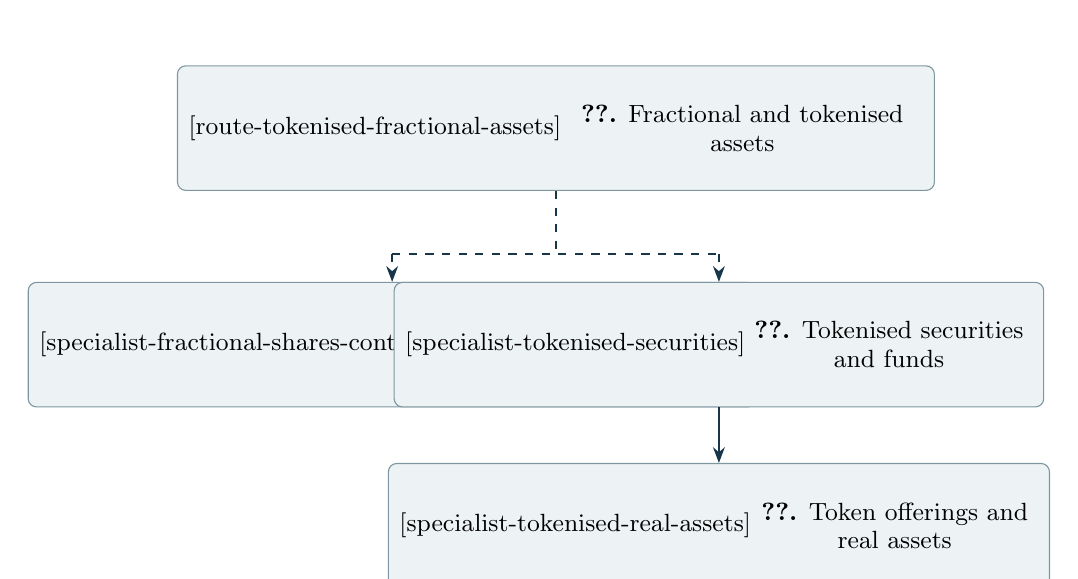
\begin{tikzpicture}[x=1cm,y=1cm]
\node[pathnode] (tokenised-fractional-assets) at (2.08,0) {\MeasurePathNode{4.6cm}{\textbf{\ref*{route-tokenised-fractional-assets}.} Fractional and tokenised assets}\hyperref[route-tokenised-fractional-assets]{\parbox[c][\pathnodeheight][c]{4.6cm}{\centering \textbf{\ref*{route-tokenised-fractional-assets}.} Fractional and tokenised assets}}};
\node[pathnode] (fractional-shares-contracts) at (0.00,-2.75) {\MeasurePathNode{3.65cm}{\textbf{\ref*{specialist-fractional-shares-contracts}.} Fractional shares and small contracts}\hyperref[specialist-fractional-shares-contracts]{\parbox[c][\pathnodeheight][c]{3.65cm}{\centering \textbf{\ref*{specialist-fractional-shares-contracts}.} Fractional shares and small contracts}}};
\node[pathnode] (tokenised-securities) at (4.15,-2.75) {\MeasurePathNode{3.65cm}{\textbf{\ref*{specialist-tokenised-securities}.} Tokenised securities and funds}\hyperref[specialist-tokenised-securities]{\parbox[c][\pathnodeheight][c]{3.65cm}{\centering \textbf{\ref*{specialist-tokenised-securities}.} Tokenised securities and funds}}};
\node[pathnode] (tokenised-real-assets) at (4.15,-5.05) {\MeasurePathNode{3.65cm}{\textbf{\ref*{specialist-tokenised-real-assets}.} Token offerings and real assets}\hyperref[specialist-tokenised-real-assets]{\parbox[c][\pathnodeheight][c]{3.65cm}{\centering \textbf{\ref*{specialist-tokenised-real-assets}.} Token offerings and real assets}}};
\draw[entryline] (tokenised-fractional-assets.south) -- (2.08,-1.60);
\draw[entryline] (0.00,-1.60) -- (4.15,-1.60);
\draw[entryarrow] (0.00,-1.60) -- (fractional-shares-contracts.north);
\draw[entryarrow] (4.15,-1.60) -- (tokenised-securities.north);
\draw[patharrow] (tokenised-securities.south) -- (tokenised-real-assets.north);
\end{tikzpicture}\end{center}
\textbf{Overview checkpoint.} A section capstone: complete it after \hyperref[specialist-fractional-shares-contracts]{\ref*{specialist-fractional-shares-contracts}} and \hyperref[specialist-tokenised-securities]{\ref*{specialist-tokenised-securities}}.

\textbf{Bring these foundations with you.}\begin{itemize}
\item \hyperref[specialist-market-structure-execution-quality]{Market structure rules, fees and execution quality} --- needed by \hyperref[specialist-fractional-shares-contracts]{Fractional shares and small contracts}.
\item \hyperref[specialist-stablecoin-tokenisation]{Stablecoins and tokenised bonds} --- needed by \hyperref[specialist-tokenised-securities]{Tokenised securities and funds}.
\end{itemize}\hyperref[learning-map]{Return to the whole-guide DAG.}
\Needspace{12\baselineskip}
\subsection{Fractional shares, odd lots and smaller contracts: retail access and market data}\label{specialist-fractional-shares-contracts}
\textbf{Specialist pathway.} In \hyperref[route-tokenised-fractional-assets]{Fractional and tokenised assets: fractional shares, tokenised securities and real-world assets}.

\textbf{Outcome.} Explain how fractional and dollar-based orders are executed and reported, what odd lots and tiny trades do to market data, price discovery and volume, and why smaller option and futures contracts have succeeded or failed.

\textbf{Prerequisites.} Fractional and tokenised assets overview; Market structure rules, fees and execution quality for off-exchange execution, the NBBO, order-execution reports and Bartlett, McCrary and O'Hara on odd-lot quotes.

\textbf{Review first.} \hyperref[route-tokenised-fractional-assets]{Fractional and tokenised assets: fractional shares, tokenised securities and real-world assets}; \hyperref[specialist-market-structure-execution-quality]{Market structure rules, fees and execution quality}.

\textbf{Required readings, in order}
\begin{enumerate}\raggedright
\Needspace{5\baselineskip}\item \href{institutional_quantitative_finance_reading_list.pdf\#ft-da-fang-lin-2025}{Zhi Da, Vivian W. Fang and Wenwei Lin, ``Fractional Trading''}\CataloguePage{154}\NoteKey{ft-da-fang-lin-2025}\par \textbf{Evidence.} Measure how fractional trading opened high-priced stocks to small investors and fed price pressure.
\Needspace{5\baselineskip}\item \href{institutional_quantitative_finance_reading_list.pdf\#ft-bartlett-mccrary-ohara-2024}{Robert P. Bartlett, Justin McCrary and Maureen O'Hara, ``Tiny trades, big questions: Fractional shares''}\CataloguePage{154}\NoteKey{ft-bartlett-mccrary-ohara-2024}\par \textbf{Data.} Identify fractional trades on the tape and their information content.
\Needspace{5\baselineskip}\item \href{institutional_quantitative_finance_reading_list.pdf\#ft-bartlett-mccrary-ohara-2025}{Robert Bartlett, Justin McCrary and Maureen O’Hara, ``A Fractional Solution to a Stock Market Mystery''}\CataloguePage{154}\NoteKey{ft-bartlett-mccrary-ohara-2025}\par \textbf{Data.} See how rounding fractional trades up created phantom volume in Berkshire Hathaway A.
\Needspace{5\baselineskip}\item \href{institutional_quantitative_finance_reading_list.pdf\#ft-nyse-fractional-2026}{NYSE Research (Intercontinental Exchange), Fractional Reporting: Early Findings}\CataloguePage{155}\NoteKey{ft-nyse-fractional-2026}\par \textbf{Data.} Read the first evidence after FINRA's February 2026 switch to decimal trade reporting.
\Needspace{5\baselineskip}\item \href{institutional_quantitative_finance_reading_list.pdf\#ft-ohara-yao-ye-2014}{Maureen O'Hara, Chen Yao and Mao Ye, ``What's Not There: Odd Lots and Market Data''}\CataloguePage{155}\NoteKey{ft-ohara-yao-ye-2014}\par \textbf{Evidence.} Measure the trading and price discovery that odd lots contribute.
\Needspace{5\baselineskip}\item \href{institutional_quantitative_finance_reading_list.pdf\#ft-battalio-2016}{Robert Battalio, Shane A. Corwin and Robert Jennings, ``Unrecognized Odd Lot Liquidity Supply: A Hidden Trading Cost for High Priced Stocks''}\CataloguePage{155}\NoteKey{ft-battalio-2016}\par \textbf{Evidence.} Price the cost of unprotected odd-lot quotes in high-priced stocks.
\Needspace{5\baselineskip}\item \href{institutional_quantitative_finance_reading_list.pdf\#ft-iosco-neobrokers-2025}{Board of the International Organization of Securities Commissions (IOSCO), Neo-Brokers: Final Report (FR/18/25)}\CataloguePage{155}\NoteKey{ft-iosco-neobrokers-2025}\par \textbf{Regulation.} Review the conduct issues of the app-based brokers that offer fractional trading.
\Needspace{5\baselineskip}\item \href{institutional_quantitative_finance_reading_list.pdf\#ft-sec-mini-options-2012}{U.S. Securities and Exchange Commission, Order Granting Accelerated Approval \ldots\ to List and Trade Option Contracts Overlying 10 Shares of Certain Securities (Release 34-67948); MIAX, rule change deleting mini-options (Release 34-101191)}\CataloguePage{155}\NoteKey{ft-sec-mini-options-2012}\par \textbf{Mechanics.} Compare the case made for 10-share mini options with their later delisting.
\Needspace{5\baselineskip}\item \href{institutional_quantitative_finance_reading_list.pdf\#ft-kurov-lasser-2004}{Alexander Kurov and Dennis J. Lasser, ``Price Dynamics in the Regular and E-Mini Futures Markets''}\CataloguePage{155}\NoteKey{ft-kurov-lasser-2004}\par \textbf{Evidence.} See how a smaller futures contract came to lead price discovery.
\end{enumerate}
\Needspace{5\baselineskip}\textbf{Checkpoint.} For 20 stocks priced above USD 500 and 20 below USD 50, measure the share of trades below one share, of odd-lot trades and of odd-lot quotes inside the NBBO in the month before and the month after 23 February 2026, when decimal reporting began. Reconstruct one dollar-based retail order from its fractional and whole-share executions. For options, compare the premium, margin and quoted spread of a standard contract with what a 10-share contract would have cost, and set the 2012 case for mini options against the reasons given for deleting them.

\textbf{Optional branches.} \href{institutional_quantitative_finance_reading_list.pdf\#s6-pfof}{Relate retail order flow and payment for order flow to execution quality.}\BranchPage{152} \href{institutional_quantitative_finance_reading_list.pdf\#ex-hasbrouck-2003}{Compare price discovery in E-mini futures, ETFs and the cash index.}\BranchPage{174}
\par{\small \hyperref[learning-map]{Learning pathway DAG} \textbar{} \hyperref[route-tokenised-fractional-assets]{Section overview} \textbar{} \hyperref[map-tokenised-fractional-assets]{Section DAG}\NoteKey{fractional-shares-contracts}}
\Needspace{12\baselineskip}
\subsection{Tokenised securities and funds: legal form, trading venues and settlement}\label{specialist-tokenised-securities}
\textbf{Specialist pathway.} In \hyperref[route-tokenised-fractional-assets]{Fractional and tokenised assets: fractional shares, tokenised securities and real-world assets}.

\textbf{Outcome.} Classify a tokenised security by who issues the token and what it represents, trace how it is recorded, traded and settled under the 2025--2026 US and EU frameworks, and estimate the settlement gains and new risks.

\textbf{Prerequisites.} Fractional and tokenised assets overview; Stablecoins and tokenised bonds (30.1) for settlement assets, tokenised bonds and tokenised money market funds. Automated market makers (32.1) helps for the 2026 exemption for AMM venues.

\textbf{Review first.} \hyperref[route-tokenised-fractional-assets]{Fractional and tokenised assets: fractional shares, tokenised securities and real-world assets}; \hyperref[specialist-stablecoin-tokenisation]{Stablecoins and tokenised bonds}.

\textbf{Required readings, in order}
\begin{enumerate}\raggedright
\Needspace{5\baselineskip}\item \href{institutional_quantitative_finance_reading_list.pdf\#tk-chiu-koeppl-2019}{Jonathan Chiu and Thorsten V. Koeppl, ``Blockchain-Based Settlement for Asset Trading''}\CataloguePage{490}\NoteKey{tk-chiu-koeppl-2019}\par \textbf{Theory.} Estimate the settlement gains and costs of trading securities on a blockchain.
\Needspace{5\baselineskip}\item \href{institutional_quantitative_finance_reading_list.pdf\#tk-sec-tokenized-statement-2026}{U.S. Securities and Exchange Commission, Divisions of Corporation Finance, Investment Management and Trading and Markets, Statement on Tokenized Securities}\CataloguePage{490}\NoteKey{tk-sec-tokenized-statement-2026}\par \textbf{Regulation.} Classify issuer-sponsored, custodial and synthetic tokenised securities.
\Needspace{5\baselineskip}\item \href{institutional_quantitative_finance_reading_list.pdf\#tk-erc3643}{Joachim Lebrun, Tony Malghem, Kevin Thizy, Luc Falempin and Adam Boudjemaa, ERC-3643: T-REX -- Token for Regulated EXchanges}\CataloguePage{491}\NoteKey{tk-erc3643}\par \textbf{Mechanics.} See how eligibility checks and transfer restrictions are coded into a permissioned security token.
\Needspace{5\baselineskip}\item \href{institutional_quantitative_finance_reading_list.pdf\#tk-dtc-nal-2025}{U.S. Securities and Exchange Commission, Division of Trading and Markets, No-Action Letter to The Depository Trust Company on the DTCC Tokenization Services}\CataloguePage{491}\NoteKey{tk-dtc-nal-2025}\par \textbf{Mechanics.} Follow how DTC entitlements are tokenised and redeemed in the pilot.
\Needspace{5\baselineskip}\item \href{institutional_quantitative_finance_reading_list.pdf\#tk-nasdaq-tokenized-2026}{U.S. Securities and Exchange Commission, Order Approving a Proposed Rule Change \ldots\ to Enable the Trading of Securities on the Exchange in Tokenized Form (Release 34-105047)}\CataloguePage{491}\NoteKey{tk-nasdaq-tokenized-2026}\par \textbf{Regulation.} See the conditions for tokenised shares to trade on the same book as traditional shares.
\Needspace{5\baselineskip}\item \href{institutional_quantitative_finance_reading_list.pdf\#tk-sec-tsv-2026}{U.S. Securities and Exchange Commission, Order Granting Temporary Conditional Exemptive Relief \ldots\ for the Use of Certain Distributed Ledger Trading Venues for Tokenized NMS Stocks (Release 34-106402)}\CataloguePage{491}\NoteKey{tk-sec-tsv-2026}\par \textbf{Regulation.} Read the 2026 conditions for trading tokenised stocks in permissioned AMM pools.
\Needspace{5\baselineskip}\item \href{institutional_quantitative_finance_reading_list.pdf\#tk-esma-dltr-2025}{European Securities and Markets Authority, Report on the Functioning and Review of the DLT Pilot Regime (ESMA75-117376770-460)}\CataloguePage{491}\NoteKey{tk-esma-dltr-2025}\par \textbf{Evidence.} Review what the EU DLT Pilot Regime produced and why uptake was limited.
\end{enumerate}
\Needspace{5\baselineskip}\textbf{Checkpoint.} Trace one Russell 1000 stock in three tokenised forms: a DTC tokenised entitlement, a tokenised share traded on Nasdaq, and a third-party custodial or synthetic token traded on a crypto venue. For each, record the master securityholder file, the transfer restrictions coded in the token, the settlement asset and timing, the handling of a dividend, and the holder's claim in the custodian's insolvency; then measure the price gap between the third-party token and the share over one weekend and one trading halt.

\textbf{Optional branches.} \href{institutional_quantitative_finance_reading_list.pdf\#section.18.6}{Review AMM pricing and liquidity in the catalogue before applying it to tokenised stocks.}\BranchPage{477}
\par{\small \hyperref[learning-map]{Learning pathway DAG} \textbar{} \hyperref[route-tokenised-fractional-assets]{Section overview} \textbar{} \hyperref[map-tokenised-fractional-assets]{Section DAG}\NoteKey{tokenised-securities}}
\Needspace{12\baselineskip}
\subsection{Token offerings and tokenised real assets: ICOs, security tokens, real estate, art and NFTs}\label{specialist-tokenised-real-assets}
\textbf{Specialist pathway.} In \hyperref[route-tokenised-fractional-assets]{Fractional and tokenised assets: fractional shares, tokenised securities and real-world assets}.

\textbf{Outcome.} Compare tokens with equity and debt as ways to finance a venture, measure the returns to token offerings, and assess whether fractional, tokenised ownership of property, art and other unique assets delivers diversification and liquidity or only a smaller minimum investment.

\textbf{Prerequisites.} Tokenised securities and funds (33.2). Collectibles: auction evidence and investable returns (28.5) helps for art and collectibles.

\textbf{Review first.} \hyperref[specialist-tokenised-securities]{Tokenised securities and funds: legal form, trading venues and settlement}.

\textbf{Required readings, in order}
\begin{enumerate}\raggedright
\Needspace{5\baselineskip}\item \href{institutional_quantitative_finance_reading_list.pdf\#tk-howell-2020}{Sabrina T. Howell, Marina Niessner and David Yermack, ``Initial Coin Offerings: Financing Growth with Cryptocurrency Token Sales''}\CataloguePage{492}\NoteKey{tk-howell-2020}\par \textbf{Evidence.} Relate token-offering success to disclosure, commitment and exchange listing.
\Needspace{5\baselineskip}\item \href{institutional_quantitative_finance_reading_list.pdf\#tk-benedetti-2021}{Hugo Benedetti and Leonard Kostovetsky, ``Digital Tulips? Returns to investors in initial coin offerings''}\CataloguePage{492}\NoteKey{tk-benedetti-2021}\par \textbf{Evidence.} Measure underpricing and early returns to initial coin offerings.
\Needspace{5\baselineskip}\item \href{institutional_quantitative_finance_reading_list.pdf\#tk-gan-2021}{Jingxing (Rowena) Gan, Gerry Tsoukalas and Serguei Netessine, ``Initial Coin Offerings, Speculation, and Asset Tokenization''}\CataloguePage{492}\NoteKey{tk-gan-2021}\par \textbf{Theory.} Design asset-backed token offerings and compare utility with equity tokens.
\Needspace{5\baselineskip}\item \href{institutional_quantitative_finance_reading_list.pdf\#tk-malinova-park-2023}{Katya Malinova and Andreas Park, ``Tokenomics: When Tokens Beat Equity''}\CataloguePage{492}\NoteKey{tk-malinova-park-2023}\par \textbf{Theory.} See when an optimally designed token matches or beats equity.
\Needspace{5\baselineskip}\item \href{institutional_quantitative_finance_reading_list.pdf\#tk-baum-2021}{Andrew Baum, ``Tokenization---The Future of Real Estate Investment?''}\CataloguePage{492}\NoteKey{tk-baum-2021}\par \textbf{Foundations.} Judge which real estate is suited to tokenisation and why an intermediate vehicle is usually needed.
\Needspace{5\baselineskip}\item \href{institutional_quantitative_finance_reading_list.pdf\#tk-swinkels-2023}{Laurens Swinkels, ``Empirical evidence on the ownership and liquidity of real estate tokens''}\CataloguePage{492}\NoteKey{tk-swinkels-2023}\par \textbf{Evidence.} Measure ownership, trading and price behaviour of tokenised rental homes.
\Needspace{5\baselineskip}\item \href{institutional_quantitative_finance_reading_list.pdf\#tk-kreppmeier-2023}{Julia Kreppmeier, Ralf Laschinger, Bertram I. Steininger and Gregor Dorfleitner, ``Real estate security token offerings and the secondary market: Driven by crypto hype or fundamentals?''}\CataloguePage{493}\NoteKey{tk-kreppmeier-2023}\par \textbf{Evidence.} Relate real estate token offerings and trading to property fundamentals and crypto sentiment.
\Needspace{5\baselineskip}\item \href{institutional_quantitative_finance_reading_list.pdf\#w5-whitaker-kraussl-fractional}{Amy Whitaker and Roman Kräussl, ``Fractional Equity, Blockchain, and the Future of Creative Work''}\CataloguePage{429}\NoteKey{w5-whitaker-kraussl-fractional}\par \textbf{Theory.} Apply fractional equity to artists' future work and the art market.
\Needspace{5\baselineskip}\item \href{institutional_quantitative_finance_reading_list.pdf\#tk-kraussl-tugnetti-2024}{Roman Kräussl and Alessandro Tugnetti, ``Non-Fungible Tokens (NFTs): A Review of Pricing Determinants, Applications and Opportunities''}\CataloguePage{493}\NoteKey{tk-kraussl-tugnetti-2024}\par \textbf{Valuation.} Survey NFT pricing models and the determinants of unique-token values.
\end{enumerate}
\Needspace{5\baselineskip}\textbf{Checkpoint.} For ten tokenised single-family homes, compare token price changes with the local house price index, count holders and trades, and estimate the discount or premium of secondary trades to appraised value. For one token offering, set out the token's cash-flow and governance rights against equity, following Malinova and Park. Conclude whether fractionalisation lowered the cost of diversification or only the minimum investment.

\textbf{Optional branches.} \href{institutional_quantitative_finance_reading_list.pdf\#tk-gryglewicz-2021}{Model when token financing beats equity for a platform.}\BranchPage{492} \href{institutional_quantitative_finance_reading_list.pdf\#section.16.5}{Use the catalogue collectibles section for auction evidence and investable returns.}\BranchPage{427}
\par{\small \hyperref[learning-map]{Learning pathway DAG} \textbar{} \hyperref[route-tokenised-fractional-assets]{Section overview} \textbar{} \hyperref[map-tokenised-fractional-assets]{Section DAG}\NoteKey{tokenised-real-assets}}
\clearpage
\section{Crypto market making: order books, DEX liquidity and token market makers}\label{route-crypto-market-making}
\label{route-35}
\textbf{Learning sequence.} Order-book dealing and RFQ, order-book microstructure, token market makers and DEX liquidity provision are separate entry points; quoting strategies and learning agents build on order-book microstructure. AMM pricing and LP returns are in Section 32; exchange market quality and wash trading are in Section 31; perpetual hedging is in Section 30.

\textbf{Section goals.} Across its pathways, this section teaches you to:
\begin{itemize}[leftmargin=1.4em,itemsep=0pt,topsep=1pt]
\item quote and hedge crypto inventory through order books and requests for quote (\hyperref[specialist-crypto-dealer-rfq]{\ref*{specialist-crypto-dealer-rfq}})
\item estimate fee, impact, latency and adverse-selection terms from a venue's data (\hyperref[specialist-crypto-mm-microstructure]{\ref*{specialist-crypto-mm-microstructure}})
\item read token market-making agreements and tell liquidity provision from manipulation (\hyperref[specialist-token-market-makers]{\ref*{specialist-token-market-makers}})
\item design and evaluate active AMM liquidity strategies (\hyperref[specialist-dex-liquidity-provision]{\ref*{specialist-dex-liquidity-provision}})
\item build and backtest model-based and learning market makers (\hyperref[specialist-crypto-mm-strategies]{\ref*{specialist-crypto-mm-strategies}})
\end{itemize}
\textbf{Overview outcome.} Cost a day of two-sided liquidity on a centralised order book and in a concentrated-liquidity AMM pool, including fees, adverse selection, repositioning, inventory hedging and capital, and say which fills and costs could not be observed.

\textbf{Prerequisites.} Market microstructure and market making (Section 18) and Crypto settlement, venues and derivatives (Section 30). On-chain protocols (Section 32) for the DEX pathway, and Crypto exchange market quality (31.2) for token market makers.

\textbf{Review first.} \hyperref[route-execution-market-making]{Market microstructure and market making}; \hyperref[route-digital-assets-prediction-markets]{Crypto settlement, venues and derivatives}.

\textbf{Required readings, in order}
\begin{enumerate}\raggedright
\Needspace{5\baselineskip}\item \href{institutional_quantitative_finance_reading_list.pdf\#crypto-cartea}{Álvaro Cartea, Sebastian Jaimungal and José Penalva, \emph{Algorithmic and High-Frequency Trading}}\CataloguePage{146}\NoteKey{crypto-cartea}\par Learn the inventory, adverse-selection and execution models that every crypto quoting strategy adapts.
\Needspace{5\baselineskip}\item \href{institutional_quantitative_finance_reading_list.pdf\#s6-easley}{David Easley, Maureen O'Hara, Songshan Yang and Zhibai Zhang, ``Microstructure and market dynamics in crypto markets''; April 2024 draft; 2025 SSRN version}\CataloguePage{439}\NoteKey{s6-easley}\par See how standard microstructure measures behave in crypto markets before quoting one.
\Needspace{5\baselineskip}\item \href{institutional_quantitative_finance_reading_list.pdf\#oc-aoyagi-ito-2025}{Jun Aoyagi and Yuki Ito, ``Coexisting Exchange Platforms: Limit Order Books and Automated Market Makers''}\CataloguePage{480}\NoteKey{oc-aoyagi-ito-2025}\par Compare a limit order book and an AMM side by side, and how liquidity moves between them.
\Needspace{5\baselineskip}\item \href{institutional_quantitative_finance_reading_list.pdf\#w5-barbon-ranaldo-quality}{Andrea Barbon and Angelo Ranaldo, ``On the quality of cryptocurrency markets: Centralized versus decentralized exchanges''}\CataloguePage{477}\NoteKey{w5-barbon-ranaldo-quality}\par Measure trading costs and price efficiency on centralised and decentralised venues on the same assets.
\end{enumerate}
\Needspace{5\baselineskip}\textbf{Checkpoint, a section capstone: complete it after \hyperref[specialist-crypto-mm-microstructure]{\ref*{specialist-crypto-mm-microstructure}} and \hyperref[specialist-dex-liquidity-provision]{\ref*{specialist-dex-liquidity-provision}}.} For one token pair traded on a centralised order book and in a Uniswap v3 pool, cost a day of USD 100,000 two-sided liquidity on each: maker fees or rebates, adverse selection from markouts, gas and repositioning for the LP, the cost of hedging inventory on a perpetual, and capital locked. State which quotes you could actually have been filled at, and which costs you could not observe.

\textbf{Optional branches.} \href{institutional_quantitative_finance_reading_list.pdf\#alpha-crypto-data}{Start from the exchange-API and connector entries before collecting order-book data.}\BranchPage{529}
\par\textbf{Continue in this section.} \hyperref[specialist-crypto-dealer-rfq]{Crypto order-book dealing and RFQ}; \hyperref[specialist-crypto-mm-microstructure]{Crypto order-book microstructure for market makers: fees, impact, latency and order flow}; \hyperref[specialist-token-market-makers]{Token market makers: issuer agreements, listings and manipulation}; \hyperref[specialist-dex-liquidity-provision]{DEX liquidity provision strategies: fee tiers, repositioning and just-in-time liquidity}; \hyperref[specialist-crypto-mm-strategies]{Crypto market-making strategies: inventory control, learning agents and backtests}.
\par{\small \hyperref[learning-map]{Learning pathway DAG} \textbar{} \hyperref[map-crypto-market-making]{Section DAG}\NoteKey{crypto-market-making}}
\clearpage
\subsection*{Crypto market making: order books, DEX liquidity and token market makers: pathway DAG}\phantomsection\label{map-crypto-market-making}
\addcontentsline{toc}{subsection}{Crypto market making: order books, DEX liquidity and token market makers: pathway DAG}
Start with the section overview's readings, for orientation. Solid arrows show prerequisites within this section. Dashed connectors identify entry points with no further prerequisite in this section; the linked foundations below still apply. Follow the arrows for dependencies and the subsection numbers for reading order. Every node is clickable.
\begin{center}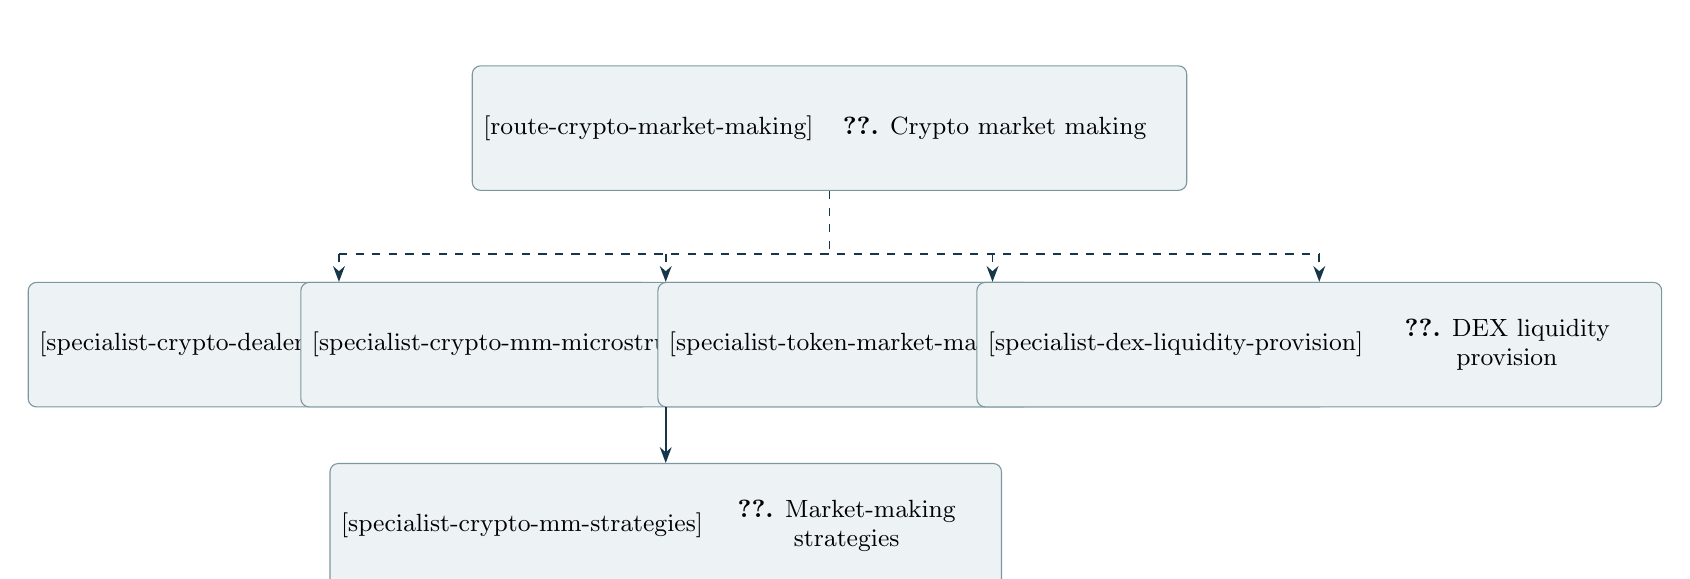
\begin{tikzpicture}[x=1cm,y=1cm]
\node[pathnode] (crypto-market-making) at (6.23,0) {\MeasurePathNode{4.6cm}{\textbf{\ref*{route-crypto-market-making}.} Crypto market making}\hyperref[route-crypto-market-making]{\parbox[c][\pathnodeheight][c]{4.6cm}{\centering \textbf{\ref*{route-crypto-market-making}.} Crypto market making}}};
\node[pathnode] (crypto-dealer-rfq) at (0.00,-2.75) {\MeasurePathNode{3.65cm}{\textbf{\ref*{specialist-crypto-dealer-rfq}.} Crypto dealing and RFQ}\hyperref[specialist-crypto-dealer-rfq]{\parbox[c][\pathnodeheight][c]{3.65cm}{\centering \textbf{\ref*{specialist-crypto-dealer-rfq}.} Crypto dealing and RFQ}}};
\node[pathnode] (crypto-mm-microstructure) at (4.15,-2.75) {\MeasurePathNode{3.65cm}{\textbf{\ref*{specialist-crypto-mm-microstructure}.} Order-book microstructure}\hyperref[specialist-crypto-mm-microstructure]{\parbox[c][\pathnodeheight][c]{3.65cm}{\centering \textbf{\ref*{specialist-crypto-mm-microstructure}.} Order-book microstructure}}};
\node[pathnode] (token-market-makers) at (8.30,-2.75) {\MeasurePathNode{3.65cm}{\textbf{\ref*{specialist-token-market-makers}.} Token market makers}\hyperref[specialist-token-market-makers]{\parbox[c][\pathnodeheight][c]{3.65cm}{\centering \textbf{\ref*{specialist-token-market-makers}.} Token market makers}}};
\node[pathnode] (dex-liquidity-provision) at (12.45,-2.75) {\MeasurePathNode{3.65cm}{\textbf{\ref*{specialist-dex-liquidity-provision}.} DEX liquidity provision}\hyperref[specialist-dex-liquidity-provision]{\parbox[c][\pathnodeheight][c]{3.65cm}{\centering \textbf{\ref*{specialist-dex-liquidity-provision}.} DEX liquidity provision}}};
\node[pathnode] (crypto-mm-strategies) at (4.15,-5.05) {\MeasurePathNode{3.65cm}{\textbf{\ref*{specialist-crypto-mm-strategies}.} Market-making strategies}\hyperref[specialist-crypto-mm-strategies]{\parbox[c][\pathnodeheight][c]{3.65cm}{\centering \textbf{\ref*{specialist-crypto-mm-strategies}.} Market-making strategies}}};
\draw[entryline] (crypto-market-making.south) -- (6.23,-1.60);
\draw[entryline] (0.00,-1.60) -- (12.45,-1.60);
\draw[entryarrow] (0.00,-1.60) -- (crypto-dealer-rfq.north);
\draw[entryarrow] (4.15,-1.60) -- (crypto-mm-microstructure.north);
\draw[entryarrow] (8.30,-1.60) -- (token-market-makers.north);
\draw[entryarrow] (12.45,-1.60) -- (dex-liquidity-provision.north);
\draw[patharrow] (crypto-mm-microstructure.south) -- (crypto-mm-strategies.north);
\end{tikzpicture}\end{center}
\textbf{Overview checkpoint.} A section capstone: complete it after \hyperref[specialist-crypto-mm-microstructure]{\ref*{specialist-crypto-mm-microstructure}} and \hyperref[specialist-dex-liquidity-provision]{\ref*{specialist-dex-liquidity-provision}}.

\textbf{Bring these foundations with you.}\begin{itemize}
\item \hyperref[route-execution-market-making]{Market microstructure and market making} --- needed by \hyperref[specialist-crypto-dealer-rfq]{Crypto dealing and RFQ}.
\item \hyperref[specialist-fx-dealer-market-making]{FX dealing: internalisation, last look and hedging} --- needed by \hyperref[specialist-crypto-dealer-rfq]{Crypto dealing and RFQ}.
\item \hyperref[specialist-market-making-lob]{Market making, queues and limit-order-book models} --- needed by \hyperref[specialist-crypto-mm-microstructure]{Order-book microstructure}.
\item \hyperref[specialist-crypto-exchange-market-quality]{Crypto exchange market quality: liquidity, fake volume and manipulation} --- needed by \hyperref[specialist-token-market-makers]{Token market makers}.
\item \hyperref[specialist-amm-lending]{Automated market makers: pricing, routing and liquidity-provider returns} --- needed by \hyperref[specialist-dex-liquidity-provision]{DEX liquidity provision}.
\item \hyperref[specialist-reinforcement-learning-trading]{Reinforcement learning for trading, hedging and execution} --- needed by \hyperref[specialist-crypto-mm-strategies]{Market-making strategies}.
\end{itemize}\hyperref[learning-map]{Return to the whole-guide DAG.}
\Needspace{12\baselineskip}
\subsection{Crypto order-book dealing and RFQ}\label{specialist-crypto-dealer-rfq}
\textbf{Specialist pathway.} In \hyperref[route-crypto-market-making]{Crypto market making: order books, DEX liquidity and token market makers}.

\textbf{Outcome.} Quote spot or perpetual inventory with a causal reference price and defensible conditional fills, then decide when to internalise or externally hedge the resulting exposure.

\textbf{Prerequisites.} Crypto market making overview; Market microstructure and market making; FX dealing: internalisation, last look and hedging; order-book event reconstruction, covariance risk and collateral-aware inventory accounting.

\textbf{Review first.} \hyperref[route-execution-market-making]{Market microstructure and market making}; \hyperref[specialist-fx-dealer-market-making]{FX dealing: internalisation, last look and hedging}; \hyperref[route-crypto-market-making]{Crypto market making: order books, DEX liquidity and token market makers}.

\textbf{Required readings, in order}
\begin{enumerate}\raggedright
\Needspace{5\baselineskip}\item \href{institutional_quantitative_finance_reading_list.pdf\#roadmap-multiasset-mm-closedform}{Philippe Bergault, David Evangelista, Olivier Guéant and Douglas Vieira, Closed-form Approximations in Multi-asset Market Making; Author preprint, arXiv v5}\CataloguePage{163}\NoteKey{roadmap-multiasset-mm-closedform}\par \textbf{Valuation.} Build a covariance-aware inventory quote approximation.
\Needspace{5\baselineskip}\item \href{institutional_quantitative_finance_reading_list.pdf\#roadmap-micro-price}{Sasha Stoikov, The micro-price: a high-frequency estimator of future prices; Author working paper and sample code}\CataloguePage{149}\NoteKey{roadmap-micro-price}\par \textbf{Reference price.} Fit a book-state micro-price and compare it with midpoint and weighted midpoint at causal horizons.
\Needspace{5\baselineskip}\item \href{institutional_quantitative_finance_reading_list.pdf\#catalogue-0833}{Bartosz Bieganowski and Robert \'{S}lepaczuk, ``Explainable Patterns in Cryptocurrency Microstructure''; SSRN posting, 19 February 2026}\CataloguePage{439}\NoteKey{catalogue-0833}\par \textbf{Evidence.} Treat reported cross-market microstructure patterns as a preprint hypothesis requiring replication under maker and taker fills.
\Needspace{5\baselineskip}\item \href{institutional_quantitative_finance_reading_list.pdf\#s11-r29}{Binance spot REST / WebSocket; Deribit APIs; selected BitMEX technical post; Coinbase engineering blog; OKX V5 API; OKX checksum change; Bitfinex books; Bitfinex raw books; Bitfinex checksum}\CataloguePage{476}\NoteKey{s11-r29}\par \textbf{Mechanics and implementation.} Pin venue-specific market-data, order, cancel and funding interfaces before replay.
\Needspace{5\baselineskip}\item \href{institutional_quantitative_finance_reading_list.pdf\#roadmap-hftbacktest}{HftBacktest contributors, HftBacktest: Order Fill}\CataloguePage{527}\NoteKey{roadmap-hftbacktest}\par \textbf{Simulation.} Compare queue/fill models and expose the fixed-market replay assumption before interpreting maker P\&L.
\end{enumerate}
\Needspace{5\baselineskip}\textbf{Checkpoint.} Replay one venue's sequenced book, local receive times, orders, acknowledgments, cancels, actual fills and missed fills. Build a reference price using only information available when each quote is sent. Compare independent versus covariance-aware inventory quotes, then an internalise-versus-external-hedge rule with hedge latency, basis, fees and capital limits. For RFQ, include every request and rejected quote in the denominator; if own response data are unavailable, label the acceptance experiment synthetic and do not infer realised dealer revenue. Evaluate signals conditional on fills; report markouts as diagnostics without adding them again to already marked P\&L.

\textbf{Optional branches.} \href{institutional_quantitative_finance_reading_list.pdf\#section.8.5}{Deepen replay and counterfactual market-response diagnostics.}\BranchPage{166} \href{institutional_quantitative_finance_reading_list.pdf\#section.18.10}{Compare feed implementations while preserving native sequence and gap rules.}\BranchPage{493} \href{institutional_quantitative_finance_reading_list.pdf\#roadmap-hyperliquid-hypercore-hlp}{Distinguish active HyperCore quoting from HLP vault/backstop exposure.}\BranchPage{446} \href{institutional_quantitative_finance_reading_list.pdf\#crypto-ccxt}{Prototype multi-venue market-data and order connectivity, checking each venue's endpoints and sequence rules separately.}\BranchPage{529} \href{institutional_quantitative_finance_reading_list.pdf\#crypto-hummingbot}{Study open-source connectors and market-making strategy code; add your own risk, key-management and reconciliation controls.}\BranchPage{529}
\par{\small \hyperref[learning-map]{Learning pathway DAG} \textbar{} \hyperref[route-crypto-market-making]{Section overview} \textbar{} \hyperref[map-crypto-market-making]{Section DAG}\NoteKey{crypto-dealer-rfq}}
\Needspace{12\baselineskip}
\subsection{Crypto order-book microstructure for market makers: fees, impact, latency and order flow}\label{specialist-crypto-mm-microstructure}
\textbf{Specialist pathway.} In \hyperref[route-crypto-market-making]{Crypto market making: order books, DEX liquidity and token market makers}.

\textbf{Outcome.} Estimate the fee, impact, latency and adverse-selection terms that decide whether quoting a crypto order book pays, from a venue's own data.

\textbf{Prerequisites.} Crypto market making overview; Market making, queues and limit-order-book models (18.1); order-book data handling and event-time econometrics.

\textbf{Review first.} \hyperref[route-crypto-market-making]{Crypto market making: order books, DEX liquidity and token market makers}; \hyperref[specialist-market-making-lob]{Market making, queues and limit-order-book models}.

\textbf{Required readings, in order}
\begin{enumerate}\raggedright
\Needspace{5\baselineskip}\item \href{institutional_quantitative_finance_reading_list.pdf\#mm-silantyev-2019}{Eduard Silantyev, ``Order flow analysis of cryptocurrency markets''}\CataloguePage{465}\NoteKey{mm-silantyev-2019}\par \textbf{Evidence.} Relate trade-flow and order-flow imbalance to price changes on a perpetual order book.
\Needspace{5\baselineskip}\item \href{institutional_quantitative_finance_reading_list.pdf\#mm-donier-bonart-2015}{J. Donier and J. Bonart, ``A Million Metaorder Analysis of Market Impact on the Bitcoin''}\CataloguePage{464}\NoteKey{mm-donier-bonart-2015}\par \textbf{Evidence.} Fit the square-root impact law to bitcoin metaorders and separate informed from uninformed flow.
\Needspace{5\baselineskip}\item \href{institutional_quantitative_finance_reading_list.pdf\#mm-donier-bouchaud-2015}{Jonathan Donier and Jean-Philippe Bouchaud, ``Why Do Markets Crash? Bitcoin Data Offers Unprecedented Insights''}\CataloguePage{464}\NoteKey{mm-donier-bouchaud-2015}\par \textbf{Evidence.} Link crashes to vanishing book liquidity and build an early-warning liquidity measure.
\Needspace{5\baselineskip}\item \href{institutional_quantitative_finance_reading_list.pdf\#w3-albers-latency-crypto}{Jakob Albers, Mihai Cucuringu, Sam Howison and Alexander Y. Shestopaloff, ``The good, the bad, and latency: exploratory trading on Bybit and Binance''}\CataloguePage{454}\NoteKey{w3-albers-latency-crypto}\par \textbf{Evidence.} See how latency and exploratory orders shape who trades first on Bybit and Binance.
\Needspace{5\baselineskip}\item \href{institutional_quantitative_finance_reading_list.pdf\#mm-brauneis-2022}{Alexander Brauneis, Roland Mestel, Ryan Riordan and Erik Theissen, ``The anatomy of a fee change — evidence from cryptocurrency markets''}\CataloguePage{464}\NoteKey{mm-brauneis-2022}\par \textbf{Evidence.} Trace what introducing maker fees did to spreads, depth and taker costs.
\Needspace{5\baselineskip}\item \href{institutional_quantitative_finance_reading_list.pdf\#mm-galati-2024}{Luca Galati, ``Exchange market share, market makers, and murky behavior: The impact of no-fee trading on cryptocurrency market quality''}\CataloguePage{464}\NoteKey{mm-galati-2024}\par \textbf{Evidence.} Trace what removing maker--taker fees did to market makers' spreads and customers' total costs.
\Needspace{5\baselineskip}\item \href{institutional_quantitative_finance_reading_list.pdf\#mm-bianchi-babiak-dickerson-2022}{Daniele Bianchi, Mykola Babiak and Alexander Dickerson, ``Trading volume and liquidity provision in cryptocurrency markets''}\CataloguePage{465}\NoteKey{mm-bianchi-babiak-dickerson-2022}\par \textbf{Evidence.} Measure the return to liquidity provision across pairs and where adverse selection raises it.
\end{enumerate}
\Needspace{5\baselineskip}\textbf{Checkpoint.} From one venue's sequenced book and trade feed, measure quoted and effective spreads, depth, trade-flow imbalance and markouts from five seconds to five minutes, by fee tier and time of day. Fit a square-root impact curve to reconstructed metaorders and compare it with Donier and Bonart. Reprice a passive quoting rule under the venue's fee schedule before and after one fee change, and with a 10 ms and a 100 ms latency handicap. List the edge terms you could not observe, such as queue position, hidden orders and tiered rebates.

\textbf{Optional branches.} \href{institutional_quantitative_finance_reading_list.pdf\#mm-petukhina-2021}{Profile intraday patterns in crypto volume, volatility and returns.}\BranchPage{465} \href{institutional_quantitative_finance_reading_list.pdf\#cs-aleti-mizrach-2021}{Compare spot and futures microstructure for bitcoin on regulated and offshore venues.}\BranchPage{452}
\par{\small \hyperref[learning-map]{Learning pathway DAG} \textbar{} \hyperref[route-crypto-market-making]{Section overview} \textbar{} \hyperref[map-crypto-market-making]{Section DAG}\NoteKey{crypto-mm-microstructure}}
\Needspace{12\baselineskip}
\subsection{Token market makers: issuer agreements, listings and manipulation}\label{specialist-token-market-makers}
\textbf{Specialist pathway.} In \hyperref[route-crypto-market-making]{Crypto market making: order books, DEX liquidity and token market makers}.

\textbf{Outcome.} Read a token market-making agreement and the trading it produces, and tell paid liquidity provision from wash trading and price support.

\textbf{Prerequisites.} Crypto market making overview; Crypto exchange market quality: liquidity, fake volume and manipulation (31.2) for wash-trading tests.

\textbf{Review first.} \hyperref[route-crypto-market-making]{Crypto market making: order books, DEX liquidity and token market makers}; \hyperref[specialist-crypto-exchange-market-quality]{Crypto exchange market quality: liquidity, fake volume and manipulation}.

\textbf{Required readings, in order}
\begin{enumerate}\raggedright
\Needspace{5\baselineskip}\item \href{institutional_quantitative_finance_reading_list.pdf\#mm-benedetti-nikbakht-2021}{Hugo Benedetti and Ehsan Nikbakht, ``Returns and network growth of digital tokens after cross-listings''}\CataloguePage{466}\NoteKey{mm-benedetti-nikbakht-2021}\par \textbf{Evidence.} See how much a new listing moves a token's price, volume and network growth.
\Needspace{5\baselineskip}\item \href{institutional_quantitative_finance_reading_list.pdf\#mm-sec-market-makers-2024}{US Securities and Exchange Commission, SEC Charges Three So-Called Market Makers and Nine Individuals in Crackdown on Manipulation of Crypto Assets Offered and Sold as Securities (Press Release 2024-166)}\CataloguePage{466}\NoteKey{mm-sec-market-makers-2024}\par \textbf{Case study.} Read how so-called market makers sold wash trading and artificial volume to token promoters.
\Needspace{5\baselineskip}\item \href{institutional_quantitative_finance_reading_list.pdf\#mm-sec-tai-mo-shan-2024}{US Securities and Exchange Commission, Tai Mo Shan to Pay \$123 Million for Negligently Misleading Investors About Stability of Terra USD (Press Release 2024-212)}\CataloguePage{466}\NoteKey{mm-sec-tai-mo-shan-2024}\par \textbf{Case study.} See how an option-based deal with an issuer turned peg-support trading into a misleading signal.
\Needspace{5\baselineskip}\item \href{institutional_quantitative_finance_reading_list.pdf\#w5-victor-weintraud-wash}{Friedhelm Victor and Andrea Marie Weintraud, ``Detecting and Quantifying Wash Trading on Decentralized Cryptocurrency Exchanges''}\CataloguePage{477}\NoteKey{w5-victor-weintraud-wash}\par \textbf{Evidence.} Detect wash trading on decentralised exchanges, where self-trades are visible on-chain.
\Needspace{5\baselineskip}\item \href{institutional_quantitative_finance_reading_list.pdf\#cs-iosco-cda-2023}{Board of the International Organization of Securities Commissions (IOSCO), Policy Recommendations for Crypto and Digital Asset Markets: Final Report (FR11/2023); Thematic Review of their implementation (FR/13/25)}\CataloguePage{463}\NoteKey{cs-iosco-cda-2023}\par \textbf{Regulation.} Apply the international recommendations on conflicts, market abuse and disclosure to market makers and venues.
\Needspace{5\baselineskip}\item \href{institutional_quantitative_finance_reading_list.pdf\#wide-mica}{European Parliament and Council, ``Regulation (EU) 2023/1114 on markets in crypto-assets (MiCA)''}\CataloguePage{486}\NoteKey{wide-mica}\par \textbf{Regulation.} Find the EU market-abuse rules that apply to crypto-asset trading, including manipulation.
\end{enumerate}
\Needspace{5\baselineskip}\textbf{Checkpoint.} For one mid-cap token, collect its listing announcements and any disclosed market-making agreement (token loan, call-option strikes, spread and depth targets). Measure spread, depth and volume on each venue before and after the agreement or a new listing, and screen volume with the wash-trading tests from 31.2. Write down what a legitimate agreement should require (disclosure, no self-trades, depth obligations) and which observed patterns would count against it.

\textbf{Optional branches.} \href{institutional_quantitative_finance_reading_list.pdf\#cd-celsius-examiner-2023}{See an issuer make the market in its own token with customer assets.}\BranchPage{448}
\par{\small \hyperref[learning-map]{Learning pathway DAG} \textbar{} \hyperref[route-crypto-market-making]{Section overview} \textbar{} \hyperref[map-crypto-market-making]{Section DAG}\NoteKey{token-market-makers}}
\Needspace{12\baselineskip}
\subsection{DEX liquidity provision strategies: fee tiers, repositioning and just-in-time liquidity}\label{specialist-dex-liquidity-provision}
\textbf{Specialist pathway.} In \hyperref[route-crypto-market-making]{Crypto market making: order books, DEX liquidity and token market makers}.

\textbf{Outcome.} Design and evaluate an active AMM liquidity strategy: choose fee tier and range, set a repositioning rule against gas, and account for just-in-time and private liquidity competing for the same flow.

\textbf{Prerequisites.} Crypto market making overview; Automated market makers: pricing, routing and liquidity-provider returns (32.1); block-level DEX data.

\textbf{Review first.} \hyperref[route-crypto-market-making]{Crypto market making: order books, DEX liquidity and token market makers}; \hyperref[specialist-amm-lending]{Automated market makers: pricing, routing and liquidity-provider returns}.

\textbf{Required readings, in order}
\begin{enumerate}\raggedright
\Needspace{5\baselineskip}\item \href{institutional_quantitative_finance_reading_list.pdf\#mm-fritsch-2021}{Robin Fritsch, ``Concentrated Liquidity in Automated Market Makers''}\CataloguePage{467}\NoteKey{mm-fritsch-2021}\par \textbf{Evidence.} Backtest basic concentrated-liquidity range rules as a first benchmark.
\Needspace{5\baselineskip}\item \href{institutional_quantitative_finance_reading_list.pdf\#mm-loesch-2021}{Stefan Loesch, Nate Hindman, Mark B Richardson and Nicholas Welch, ``Impermanent Loss in Uniswap v3''}\CataloguePage{467}\NoteKey{mm-loesch-2021}\par \textbf{Evidence.} Measure impermanent loss against fees for large Uniswap v3 pools.
\Needspace{5\baselineskip}\item \href{institutional_quantitative_finance_reading_list.pdf\#mm-lehar-parlour-zoican-2023}{Alfred Lehar, Christine Parlour and Marius Zoican, ``Fragmentation and optimal liquidity supply on decentralized exchanges''}\CataloguePage{466}\NoteKey{mm-lehar-parlour-zoican-2023}\par \textbf{Evidence.} See how gas costs sort large and small LPs into low- and high-fee pools.
\Needspace{5\baselineskip}\item \href{institutional_quantitative_finance_reading_list.pdf\#mm-caparros-chaudhary-klein-2023}{Basile Caparros, Amit Chaudhary and Olga Klein, ``Blockchain scaling and liquidity concentration on decentralized exchanges''}\CataloguePage{467}\NoteKey{mm-caparros-chaudhary-klein-2023}\par \textbf{Evidence.} Use cheaper gas on rollups to show how repositioning frequency concentrates liquidity.
\Needspace{5\baselineskip}\item \href{institutional_quantitative_finance_reading_list.pdf\#mm-zhu-2025}{Brian Zhu, Dingyue Liu, Xin Wan, Gordon Liao, Ciamac C. Moallemi and Brad Bachu, ``What Drives Liquidity on Decentralized Exchanges? Evidence from the Uniswap Protocol''}\CataloguePage{467}\NoteKey{mm-zhu-2025}\par \textbf{Evidence.} Decompose DEX depth into locked value and concentration, including private market makers on aggregators.
\Needspace{5\baselineskip}\item \href{institutional_quantitative_finance_reading_list.pdf\#w3-chen-dex-liquidity-info}{Tian Chen, Jun Deng, Jing Nie, Bin Zou and Qi Fu, ``Liquidity provision and its information content in decentralized markets''}\CataloguePage{479}\NoteKey{w3-chen-dex-liquidity-info}\par \textbf{Evidence.} Test whether LP actions carry information about future prices.
\Needspace{5\baselineskip}\item \href{institutional_quantitative_finance_reading_list.pdf\#mm-capponi-jia-zhu-2023}{Agostino Capponi, Ruizhe Jia and Brian Zhu, ``The Paradox Of Just-in-Time Liquidity in Decentralized Exchanges: More Providers Can Sometimes Mean Less Liquidity''}\CataloguePage{466}\NoteKey{mm-capponi-jia-zhu-2023}\par \textbf{Theory.} Model how just-in-time LPs avoid toxic flow and can crowd out passive LPs.
\Needspace{5\baselineskip}\item \href{institutional_quantitative_finance_reading_list.pdf\#mm-xiong-2023}{Xihan Xiong, Zhipeng Wang, William Knottenbelt and Michael Huth, ``Demystifying Just-in-Time (JIT) Liquidity Attacks on Uniswap V3''}\CataloguePage{467}\NoteKey{mm-xiong-2023}\par \textbf{Evidence.} Measure who runs just-in-time liquidity, what it earns and how much it dilutes passive LPs.
\Needspace{5\baselineskip}\item \href{institutional_quantitative_finance_reading_list.pdf\#mm-trotti-2025}{Bruno Llacer Trotti, Weizhao Tang, Rachid El-Azouzi, Giulia Fanti and Daniel Sadoc Menasché, ``Strategic Analysis of Just-In-Time Liquidity Provision in Concentrated Liquidity Market Makers''}\CataloguePage{467}\NoteKey{mm-trotti-2025}\par \textbf{Theory.} Solve the just-in-time LP's optimisation and its effect on slippage and passive LP profit.
\end{enumerate}
\Needspace{5\baselineskip}\textbf{Checkpoint.} Backtest three LP policies on one Uniswap v3 pool and its other fee tier: a wide passive range, a narrow range rebalanced on a schedule, and a narrow range rebalanced when price exits, each with gas, rebalancing swap costs and an optional perpetual hedge. Report fees, loss-versus-rebalancing, gas and hedge P\&L separately, and the share of the pool's fees taken by just-in-time positions. Use block-level data, and say where missing mempool or private order-flow data mean just-in-time or private market makers are ignored.

\textbf{Optional branches.} \href{institutional_quantitative_finance_reading_list.pdf\#mm-wan-adams-2023}{Compare a protocol team's finding that just-in-time liquidity is rare and improves execution.}\BranchPage{467} \href{institutional_quantitative_finance_reading_list.pdf\#roadmap-cex-dex-extracted}{Estimate what CEX--DEX arbitrage takes from LPs, the flow an LP hedge trades against.}\BranchPage{439}
\par{\small \hyperref[learning-map]{Learning pathway DAG} \textbar{} \hyperref[route-crypto-market-making]{Section overview} \textbar{} \hyperref[map-crypto-market-making]{Section DAG}\NoteKey{dex-liquidity-provision}}
\Needspace{12\baselineskip}
\subsection{Crypto market-making strategies: inventory control, learning agents and backtests}\label{specialist-crypto-mm-strategies}
\textbf{Specialist pathway.} In \hyperref[route-crypto-market-making]{Crypto market making: order books, DEX liquidity and token market makers}.

\textbf{Outcome.} Build, backtest and compare a model-based and a learning market maker on crypto data without letting the simulator flatter either one.

\textbf{Prerequisites.} Crypto order-book microstructure for market makers; Reinforcement learning for trading, hedging and execution (4.5); stochastic control for inventory models.

\textbf{Review first.} \hyperref[specialist-crypto-mm-microstructure]{Crypto order-book microstructure for market makers: fees, impact, latency and order flow}; \hyperref[specialist-reinforcement-learning-trading]{Reinforcement learning for trading, hedging and execution}.

\textbf{Required readings, in order}
\begin{enumerate}\raggedright
\Needspace{5\baselineskip}\item \href{institutional_quantitative_finance_reading_list.pdf\#mm-sadighian-2019}{Jonathan Sadighian, ``Deep Reinforcement Learning in Cryptocurrency Market Making''}\CataloguePage{465}\NoteKey{mm-sadighian-2019}\par \textbf{Methods.} Set up a reinforcement-learning market maker: state, actions, reward and inventory control.
\Needspace{5\baselineskip}\item \href{institutional_quantitative_finance_reading_list.pdf\#mm-he-zheng-yang-2023}{Jiafa He, Cong Zheng and Can Yang, ``Integrating Tick-level Data and Periodical Signal for High-frequency Market Making''}\CataloguePage{465}\NoteKey{mm-he-zheng-yang-2023}\par \textbf{Methods.} Add tick-level data and periodic signals to a learning quoting agent.
\Needspace{5\baselineskip}\item \href{institutional_quantitative_finance_reading_list.pdf\#mm-schnaubelt-2022}{Matthias Schnaubelt, ``Deep reinforcement learning for the optimal placement of cryptocurrency limit orders''}\CataloguePage{465}\NoteKey{mm-schnaubelt-2022}\par \textbf{Methods.} Train limit-order placement in a virtual exchange on 18 months of crypto book data.
\Needspace{5\baselineskip}\item \href{institutional_quantitative_finance_reading_list.pdf\#crypto-nautilus}{NautilusTrader}\CataloguePage{527}\NoteKey{crypto-nautilus}\par \textbf{Implementation.} Run the same strategy code in event-driven backtest and live modes.
\Needspace{5\baselineskip}\item \href{institutional_quantitative_finance_reading_list.pdf\#crypto-cryptofeed}{Cryptofeed}\CataloguePage{529}\NoteKey{crypto-cryptofeed}\par \textbf{Data.} Collect normalised order-book and trade streams across exchanges for training and replay.
\end{enumerate}
\Needspace{5\baselineskip}\textbf{Checkpoint.} Tune one Avellaneda--Stoikov-style quoting rule and train one learning agent on the same pair. Run both in a queue-aware replay with exchange latency, fees and partial fills, then on a held-out month that contains a regime change. Report P\&L split into spread capture, inventory P\&L, fees and hedging, with inventory paths and fill rates. Treat any result from a simulator without queue position as an upper bound.

\textbf{Optional branches.} \href{institutional_quantitative_finance_reading_list.pdf\#roadmap-hftbacktest}{Compare queue and fill models before trusting a backtest of passive orders.}\BranchPage{527} \href{institutional_quantitative_finance_reading_list.pdf\#wide-gasperov-mm-review}{Check a learning market maker against the evaluation weaknesses common in the literature.}\BranchPage{164} \href{institutional_quantitative_finance_reading_list.pdf\#crypto-freqtrade}{Read an open-source bot framework for strategy plumbing, not for its performance claims.}\BranchPage{529} \href{institutional_quantitative_finance_reading_list.pdf\#mm-cartea-drissi-monga-statarb-2023}{Compare quoting with a taker strategy that trades a basket across AMM pools and an order book (35.3).}\BranchPage{466}
\par{\small \hyperref[learning-map]{Learning pathway DAG} \textbar{} \hyperref[route-crypto-market-making]{Section overview} \textbar{} \hyperref[map-crypto-market-making]{Section DAG}\NoteKey{crypto-mm-strategies}}
\clearpage
\section{Crypto trading strategies: factors, trend, arbitrage, sentiment and machine learning}\label{route-crypto-trading-strategies}
\label{route-36}
\textbf{Learning sequence.} Cross-sectional factors, trend and technical rules, statistical arbitrage, arbitrage and carry, and sentiment and event strategies are separate entry points; machine-learning prediction builds on the cross-sectional pathway. Market making is in Section 34; on-chain signals and wallet data are in Crypto signals and on-chain evidence (32.7); option and volatility strategies are in Section 30.

\textbf{Section goals.} Across its pathways, this section teaches you to:
\begin{itemize}[leftmargin=1.4em,itemsep=0pt,topsep=1pt]
\item build cross-sectional crypto factor portfolios and manage their crash risk (\hyperref[specialist-crypto-cross-section]{\ref*{specialist-crypto-cross-section}})
\item test trend, intraday momentum and technical rules with data-snooping controls (\hyperref[specialist-crypto-trend-technical]{\ref*{specialist-crypto-trend-technical}})
\item build and test crypto statistical-arbitrage strategies (\hyperref[specialist-crypto-stat-arb]{\ref*{specialist-crypto-stat-arb}})
\item train and judge machine-learning crypto return forecasts (\hyperref[specialist-crypto-ml-prediction]{\ref*{specialist-crypto-ml-prediction}})
\item size cross-exchange, triangular, funding-basis and DeFi carry trades (\hyperref[specialist-crypto-arbitrage-carry]{\ref*{specialist-crypto-arbitrage-carry}})
\item test attention, sentiment and event signals (\hyperref[specialist-crypto-sentiment-events]{\ref*{specialist-crypto-sentiment-events}})
\end{itemize}
\textbf{Overview outcome.} Choose, test and size a crypto trading strategy other than market making, separating a persistent premium from a small-coin, high-cost or sample-specific artefact.

\textbf{Prerequisites.} Crypto spot markets (Section 31); Empirical asset pricing: factor models and tests (2.3); Backtest inference, multiple testing and Sharpe-ratio statistics (3.1). Crypto perpetuals and cross-venue basis (30.2) for the carry pathway.

\textbf{Review first.} \hyperref[route-crypto-spot-markets]{Crypto spot markets: price discovery, market quality, valuation and investors}; \hyperref[specialist-empirical-asset-pricing]{Empirical asset pricing: factor models and tests}; \hyperref[specialist-backtest-inference]{Backtest inference, multiple testing and Sharpe-ratio statistics}.

\textbf{Required readings, in order}
\begin{enumerate}\raggedright
\Needspace{5\baselineskip}\item \href{institutional_quantitative_finance_reading_list.pdf\#st-borri-liu-tsyvinski-wu-2026}{Nicola Borri, Yukun Liu, Aleh Tsyvinski and Xi Wu, ``Cryptocurrency as an Investable Asset Class: Coming of Age''}\CataloguePage{469}\NoteKey{st-borri-liu-tsyvinski-wu-2026}\par Start from the stylised facts of crypto as an asset class: comparable risk-adjusted returns, a few factors, frequent jumps and blockchain information.
\Needspace{5\baselineskip}\item \href{institutional_quantitative_finance_reading_list.pdf\#st-fang-2022}{Fan Fang, Carmine Ventre, Michail Basios, Leslie Kanthan, David Martinez-Rego, Fan Wu and Lingbo Li, ``Cryptocurrency trading: a comprehensive survey''}\CataloguePage{475}\NoteKey{st-fang-2022}\par Map the crypto trading literature by strategy family, data and evaluation before choosing one.
\Needspace{5\baselineskip}\item \href{institutional_quantitative_finance_reading_list.pdf\#s6-cryptofactors}{Yukun Liu, Aleh Tsyvinski and Xi Wu, ``Common Risk Factors in Cryptocurrency''; NBER working paper}\CataloguePage{442}\NoteKey{s6-cryptofactors}\par Use the market, size and momentum factors as the benchmark every strategy must beat.
\Needspace{5\baselineskip}\item \href{institutional_quantitative_finance_reading_list.pdf\#roadmap-crypto-risks-returns}{Yukun Liu and Aleh Tsyvinski, Risks and Returns of Cryptocurrency; NBER working paper 24877}\CataloguePage{442}\NoteKey{roadmap-crypto-risks-returns}\par Relate crypto returns to standard factors, momentum and investor attention.
\Needspace{5\baselineskip}\item \href{institutional_quantitative_finance_reading_list.pdf\#s11-r27}{Kaiko, ``The Crypto Data Problem'' (source: 2023)}\CataloguePage{476}\NoteKey{s11-r27}\par Check how exchange coverage and provider choices change the price history a backtest uses.
\end{enumerate}
\Needspace{5\baselineskip}\textbf{Checkpoint.} Pick one strategy from each of two families (for example short-term reversal and a funding-basis trade). For each, write the signal, universe filter, rebalancing rule, venues and cost model before looking at returns. Backtest both over the same period with point-in-time coin lists, delisted coins, exchange fees, spreads and borrow or funding, then report returns net of costs, capacity at realistic volume shares, exposure to the market, size and momentum factors, and the number of variants you tried.

\textbf{Optional branches.} \href{institutional_quantitative_finance_reading_list.pdf\#st-trimborn-2020}{Add crypto to a multi-asset portfolio only in amounts that can actually be traded.}\BranchPage{475} \href{institutional_quantitative_finance_reading_list.pdf\#st-brauneis-mestel-2019}{Compare mean--variance crypto portfolios with the 1/N benchmark out of sample.}\BranchPage{475} \href{institutional_quantitative_finance_reading_list.pdf\#st-liu-2019}{Test common allocation models across coins against 1/N.}\BranchPage{475} \href{institutional_quantitative_finance_reading_list.pdf\#cs-platanakis-urquhart-2020}{Test bitcoin in out-of-sample stock--bond portfolios.}\BranchPage{459} \href{institutional_quantitative_finance_reading_list.pdf\#s11-r21}{Read practitioner evidence on digital assets in traditional allocations.}\BranchPage{443}
\par\textbf{Continue in this section.} \hyperref[specialist-crypto-cross-section]{Cross-sectional crypto strategies: size, momentum, reversal, value and factor momentum}; \hyperref[specialist-crypto-trend-technical]{Crypto trend following, intraday momentum, technical rules and calendar effects}; \hyperref[specialist-crypto-stat-arb]{Crypto statistical arbitrage and pairs trading}; \hyperref[specialist-crypto-ml-prediction]{Machine-learning crypto return prediction and backtest pitfalls}; \hyperref[specialist-crypto-arbitrage-carry]{Crypto arbitrage and carry: cross-exchange, triangular, funding basis and DeFi yields}; \hyperref[specialist-crypto-sentiment-events]{Attention, sentiment and event-driven crypto strategies}.
\par{\small \hyperref[learning-map]{Learning pathway DAG} \textbar{} \hyperref[map-crypto-trading-strategies]{Section DAG}\NoteKey{crypto-trading-strategies}}
\clearpage
\subsection*{Crypto trading strategies: factors, trend, arbitrage, sentiment and machine learning: pathway DAG}\phantomsection\label{map-crypto-trading-strategies}
\addcontentsline{toc}{subsection}{Crypto trading strategies: factors, trend, arbitrage, sentiment and machine learning: pathway DAG}
Start with the section overview's readings, for orientation. Solid arrows show prerequisites within this section. Dashed connectors identify entry points with no further prerequisite in this section; the linked foundations below still apply. Follow the arrows for dependencies and the subsection numbers for reading order. Every node is clickable.
\begin{center}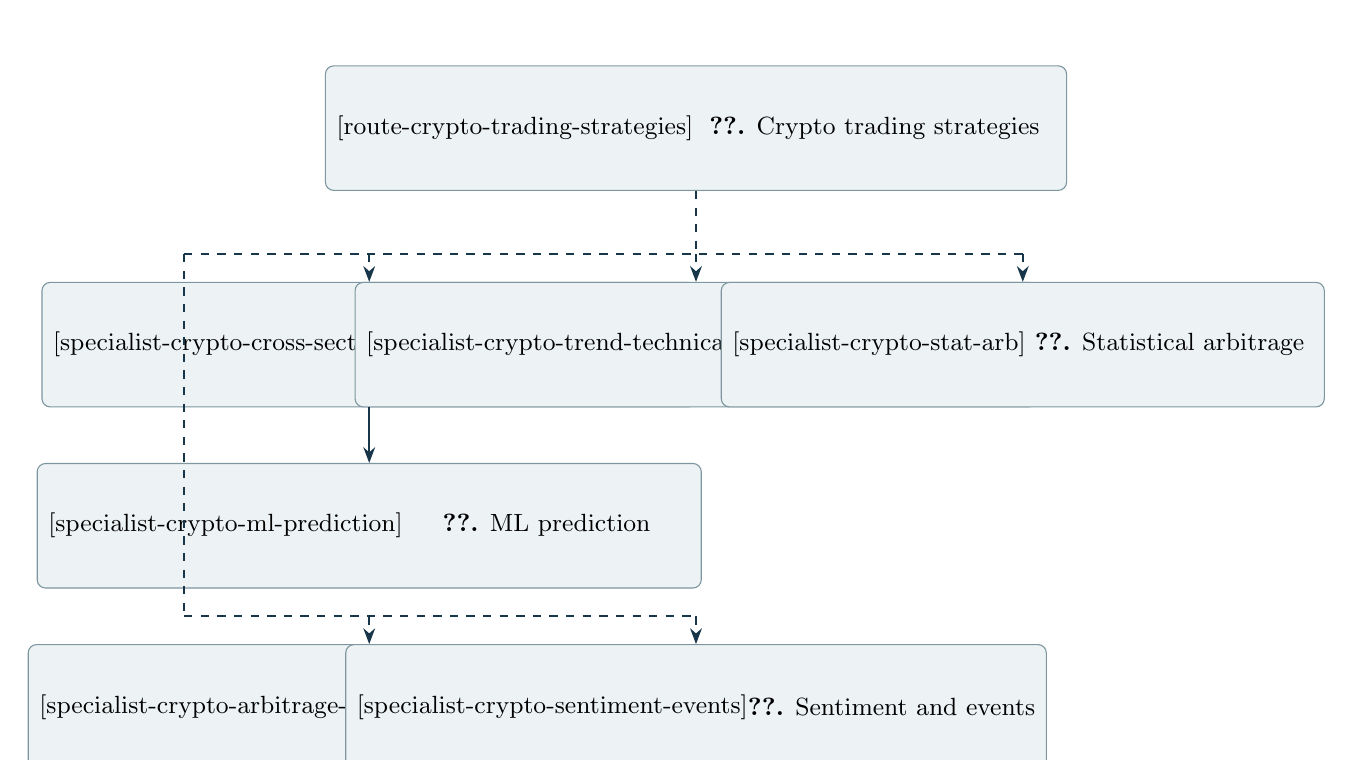
\begin{tikzpicture}[x=1cm,y=1cm]
\node[pathnode] (crypto-trading-strategies) at (4.15,0) {\MeasurePathNode{4.6cm}{\textbf{\ref*{route-crypto-trading-strategies}.} Crypto trading strategies}\hyperref[route-crypto-trading-strategies]{\parbox[c][\pathnodeheight][c]{4.6cm}{\centering \textbf{\ref*{route-crypto-trading-strategies}.} Crypto trading strategies}}};
\node[pathnode] (crypto-cross-section) at (0.00,-2.75) {\MeasurePathNode{3.65cm}{\textbf{\ref*{specialist-crypto-cross-section}.} Cross-sectional strategies}\hyperref[specialist-crypto-cross-section]{\parbox[c][\pathnodeheight][c]{3.65cm}{\centering \textbf{\ref*{specialist-crypto-cross-section}.} Cross-sectional strategies}}};
\node[pathnode] (crypto-trend-technical) at (4.15,-2.75) {\MeasurePathNode{3.65cm}{\textbf{\ref*{specialist-crypto-trend-technical}.} Trend and technical rules}\hyperref[specialist-crypto-trend-technical]{\parbox[c][\pathnodeheight][c]{3.65cm}{\centering \textbf{\ref*{specialist-crypto-trend-technical}.} Trend and technical rules}}};
\node[pathnode] (crypto-stat-arb) at (8.30,-2.75) {\MeasurePathNode{3.65cm}{\textbf{\ref*{specialist-crypto-stat-arb}.} Statistical arbitrage}\hyperref[specialist-crypto-stat-arb]{\parbox[c][\pathnodeheight][c]{3.65cm}{\centering \textbf{\ref*{specialist-crypto-stat-arb}.} Statistical arbitrage}}};
\node[pathnode] (crypto-ml-prediction) at (0.00,-5.05) {\MeasurePathNode{3.65cm}{\textbf{\ref*{specialist-crypto-ml-prediction}.} ML prediction}\hyperref[specialist-crypto-ml-prediction]{\parbox[c][\pathnodeheight][c]{3.65cm}{\centering \textbf{\ref*{specialist-crypto-ml-prediction}.} ML prediction}}};
\node[pathnode] (crypto-arbitrage-carry) at (0.00,-7.35) {\MeasurePathNode{3.65cm}{\textbf{\ref*{specialist-crypto-arbitrage-carry}.} Arbitrage and carry}\hyperref[specialist-crypto-arbitrage-carry]{\parbox[c][\pathnodeheight][c]{3.65cm}{\centering \textbf{\ref*{specialist-crypto-arbitrage-carry}.} Arbitrage and carry}}};
\node[pathnode] (crypto-sentiment-events) at (4.15,-7.35) {\MeasurePathNode{3.65cm}{\textbf{\ref*{specialist-crypto-sentiment-events}.} Sentiment and events}\hyperref[specialist-crypto-sentiment-events]{\parbox[c][\pathnodeheight][c]{3.65cm}{\centering \textbf{\ref*{specialist-crypto-sentiment-events}.} Sentiment and events}}};
\draw[entryline] (crypto-trading-strategies.south) -- (4.15,-1.60);
\draw[entryline] (-2.35,-1.60) -- (-2.35,-6.20);
\draw[entryline] (-2.35,-1.60) -- (8.30,-1.60);
\draw[entryarrow] (0.00,-1.60) -- (crypto-cross-section.north);
\draw[entryarrow] (4.15,-1.60) -- (crypto-trend-technical.north);
\draw[entryarrow] (8.30,-1.60) -- (crypto-stat-arb.north);
\draw[entryline] (-2.35,-6.20) -- (4.15,-6.20);
\draw[entryarrow] (0.00,-6.20) -- (crypto-arbitrage-carry.north);
\draw[entryarrow] (4.15,-6.20) -- (crypto-sentiment-events.north);
\draw[patharrow] (crypto-cross-section.south) -- (crypto-ml-prediction.north);
\end{tikzpicture}\end{center}
\textbf{Bring these foundations with you.}\begin{itemize}
\item \hyperref[specialist-empirical-asset-pricing]{Empirical asset pricing: factor models and tests} --- needed by \hyperref[specialist-crypto-cross-section]{Cross-sectional strategies}.
\item \hyperref[specialist-time-series-volatility]{Time-series econometrics and volatility forecasting} --- needed by \hyperref[specialist-crypto-trend-technical]{Trend and technical rules}.
\item \hyperref[specialist-statistical-arbitrage]{Statistical arbitrage and short-horizon equity strategies} --- needed by \hyperref[specialist-crypto-stat-arb]{Statistical arbitrage}.
\item \hyperref[specialist-financial-ml-evaluation]{Financial ML: information timing, uncertainty and portfolio tests} --- needed by \hyperref[specialist-crypto-ml-prediction]{ML prediction}.
\item \hyperref[specialist-backtest-inference]{Backtest inference, multiple testing and Sharpe-ratio statistics} --- needed by \hyperref[specialist-crypto-ml-prediction]{ML prediction}.
\item \hyperref[specialist-crypto-perpetuals]{Crypto perpetuals and cross-venue basis} --- needed by \hyperref[specialist-crypto-arbitrage-carry]{Arbitrage and carry}.
\item \hyperref[specialist-crypto-price-discovery]{Crypto price discovery: cross-exchange arbitrage, futures, spot ETFs and reference rates} --- needed by \hyperref[specialist-crypto-arbitrage-carry]{Arbitrage and carry}.
\item \hyperref[specialist-event-studies]{Event studies and long-run abnormal returns} --- needed by \hyperref[specialist-crypto-sentiment-events]{Sentiment and events}.
\end{itemize}\hyperref[learning-map]{Return to the whole-guide DAG.}
\Needspace{12\baselineskip}
\subsection{Cross-sectional crypto strategies: size, momentum, reversal, value and factor momentum}\label{specialist-crypto-cross-section}
\textbf{Specialist pathway.} In \hyperref[route-crypto-trading-strategies]{Crypto trading strategies: factors, trend, arbitrage, sentiment and machine learning}.

\textbf{Outcome.} Build long--short crypto portfolios on size, momentum, reversal, value and lottery-demand signals, manage their crash risk, and show which premia survive liquidity filters, costs and the choice of horizon.

\textbf{Prerequisites.} Crypto trading strategies overview; Empirical asset pricing: factor models and tests (2.3).

\textbf{Review first.} \hyperref[route-crypto-trading-strategies]{Crypto trading strategies: factors, trend, arbitrage, sentiment and machine learning}; \hyperref[specialist-empirical-asset-pricing]{Empirical asset pricing: factor models and tests}.

\textbf{Required readings, in order}
\begin{enumerate}\raggedright
\Needspace{5\baselineskip}\item \href{institutional_quantitative_finance_reading_list.pdf\#catalogue-0829}{Nicola Borri and Kirill Shakhnov, ``The Cross-Section of Cryptocurrency Returns''}\CataloguePage{451}\NoteKey{catalogue-0829}\par \textbf{Evidence.} Start from the cross-section of crypto returns and the characteristics that price it.
\Needspace{5\baselineskip}\item \href{institutional_quantitative_finance_reading_list.pdf\#st-zaremba-2021}{Adam Zaremba, Mehmet Huseyin Bilgin, Huaigang Long, Aleksander Mercik and Jan J. Szczygielski, ``Up or down? Short-term reversal, momentum, and liquidity effects in cryptocurrency markets''}\CataloguePage{468}\NoteKey{st-zaremba-2021}\par \textbf{Evidence.} See daily reversal in illiquid coins turn into momentum among the largest ones.
\Needspace{5\baselineskip}\item \href{institutional_quantitative_finance_reading_list.pdf\#st-dobrynskaya-2023}{Victoria Dobrynskaya, ``Cryptocurrency Momentum and Reversal''}\CataloguePage{468}\NoteKey{st-dobrynskaya-2023}\par \textbf{Evidence.} Map momentum up to a month and reversal beyond it across horizons.
\Needspace{5\baselineskip}\item \href{institutional_quantitative_finance_reading_list.pdf\#st-grobys-sapkota-2019}{Klaus Grobys and Niranjan Sapkota, ``Cryptocurrencies and momentum''}\CataloguePage{468}\NoteKey{st-grobys-sapkota-2019}\par \textbf{Counter-evidence.} Find no monthly momentum in a smaller 2014--2018 universe.
\Needspace{5\baselineskip}\item \href{institutional_quantitative_finance_reading_list.pdf\#s11-r06}{Klaus Grobys and Syed Jawad Hussain Shahzad, ``Cryptocurrency Momentum: Is It an Illusion?'' (SSRN: written 22 September, posted 30 November 2023); journal version}\CataloguePage{443}\NoteKey{s11-r06}\par \textbf{Counter-evidence.} Check momentum strategies for tail risk that makes their premium look larger than it is.
\Needspace{5\baselineskip}\item \href{institutional_quantitative_finance_reading_list.pdf\#cs-cong-karolyi-2026}{Lin William Cong, G. Andrew Karolyi, Ke Tang and Weiyi Zhao, ``Crypto Value, Factor Pricing, and Market Segmentation''}\CataloguePage{459}\NoteKey{cs-cong-karolyi-2026}\par \textbf{Evidence.} Add a crypto value factor and the segmentation of token categories.
\Needspace{5\baselineskip}\item \href{institutional_quantitative_finance_reading_list.pdf\#w3-fieberg-crypto-trend}{Christian Fieberg, Gerrit Liedtke, Thorsten Poddig, Thomas Walker and Adam Zaremba, ``A Trend Factor for the Cross Section of Cryptocurrency Returns''}\CataloguePage{443}\NoteKey{w3-fieberg-crypto-trend}\par \textbf{Evidence.} Combine price-trend signals into a single crypto trend factor.
\Needspace{5\baselineskip}\item \href{institutional_quantitative_finance_reading_list.pdf\#st-fieberg-factor-momentum-2023}{Christian Fieberg, Gerrit Liedtke, Daniel Metko and Adam Zaremba, ``Cryptocurrency factor momentum''}\CataloguePage{468}\NoteKey{st-fieberg-factor-momentum-2023}\par \textbf{Evidence.} Time anomalies by their own past returns and see where factor momentum comes from.
\Needspace{5\baselineskip}\item \href{institutional_quantitative_finance_reading_list.pdf\#w3-babiak-crypto-ipca}{Mykola Babiak and Daniele Bianchi, ``Mispricing and Risk Compensation in Cryptocurrency Returns''}\CataloguePage{443}\NoteKey{w3-babiak-crypto-ipca}\par \textbf{Evidence.} Separate risk compensation from mispricing with instrumented factor loadings.
\Needspace{5\baselineskip}\item \href{institutional_quantitative_finance_reading_list.pdf\#st-grobys-junttila-2021}{Klaus Grobys and Juha Junttila, ``Speculation and lottery-like demand in cryptocurrency markets''}\CataloguePage{469}\NoteKey{st-grobys-junttila-2021}\par \textbf{Evidence.} Sort coins on last week's maximum daily return and see lottery-like demand lower future returns.
\Needspace{5\baselineskip}\item \href{institutional_quantitative_finance_reading_list.pdf\#st-grobys-2025}{Klaus Grobys, James W. Kolari, Davide Sandretto, Syed Jawad H. Shahzad and Janne Äijö, ``Cryptocurrency momentum has (not) its moments''}\CataloguePage{469}\NoteKey{st-grobys-2025}\par \textbf{Risk management.} See crypto momentum crash and how volatility management limits the damage.
\end{enumerate}
\Needspace{5\baselineskip}\textbf{Checkpoint.} Using a point-in-time universe that includes dead coins, sort coins weekly on size, one-day and one-month past returns and one value proxy, with and without a liquidity filter (for example the top 100 by volume). Report long and short leg returns separately, net of spreads and fees, and alphas against the Liu--Tsyvinski--Wu factors. Show how each premium changes with the liquidity filter, the holding period and the 2018 and 2022 drawdowns, and say which legs could not have been shorted.

\textbf{Optional branches.} \href{institutional_quantitative_finance_reading_list.pdf\#st-shen-urquhart-wang-2020}{Use a market, size and reversal model as an alternative baseline.}\BranchPage{468} \href{institutional_quantitative_finance_reading_list.pdf\#st-tzouvanas-2020}{See short-horizon momentum on a dozen large coins and its diversification value.}\BranchPage{468} \href{institutional_quantitative_finance_reading_list.pdf\#st-kita-zhang-2026}{Time crypto exposure by volatility and see when the timing alpha reflects mispricing.}\BranchPage{469} \href{institutional_quantitative_finance_reading_list.pdf\#st-yadav-2025}{Test the MAX effect at an hourly horizon alongside idiosyncratic volatility and skewness.}\BranchPage{469}
\par{\small \hyperref[learning-map]{Learning pathway DAG} \textbar{} \hyperref[route-crypto-trading-strategies]{Section overview} \textbar{} \hyperref[map-crypto-trading-strategies]{Section DAG}\NoteKey{crypto-cross-section}}
\Needspace{12\baselineskip}
\subsection{Crypto trend following, intraday momentum, technical rules and calendar effects}\label{specialist-crypto-trend-technical}
\textbf{Specialist pathway.} In \hyperref[route-crypto-trading-strategies]{Crypto trading strategies: factors, trend, arbitrage, sentiment and machine learning}.

\textbf{Outcome.} Test daily and intraday time-series momentum and technical rules on crypto with data-snooping controls, and tell a tradeable trend from a calendar or sample artefact.

\textbf{Prerequisites.} Crypto trading strategies overview; Time-series econometrics and volatility forecasting (1.4). Backtest inference (3.1) for multiple-testing corrections; Trend following and managed futures (12.2) for the cross-asset version.

\textbf{Review first.} \hyperref[route-crypto-trading-strategies]{Crypto trading strategies: factors, trend, arbitrage, sentiment and machine learning}; \hyperref[specialist-time-series-volatility]{Time-series econometrics and volatility forecasting}.

\textbf{Required readings, in order}
\begin{enumerate}\raggedright
\Needspace{5\baselineskip}\item \href{institutional_quantitative_finance_reading_list.pdf\#st-detzel-2021}{Andrew Detzel, Hong Liu, Jack Strauss, Guofu Zhou and Yingzi Zhu, ``Learning and predictability via technical analysis: Evidence from bitcoin and stocks with hard‐to‐value fundamentals''}\CataloguePage{469}\NoteKey{st-detzel-2021}\par \textbf{Theory.} See why moving-average signals can predict an asset with hard-to-value fundamentals.
\Needspace{5\baselineskip}\item \href{institutional_quantitative_finance_reading_list.pdf\#st-hudson-urquhart-2021}{Robert Hudson and Andrew Urquhart, ``Technical trading and cryptocurrencies''}\CataloguePage{469}\NoteKey{st-hudson-urquhart-2021}\par \textbf{Evidence.} Test thousands of technical rules with data-snooping corrections, and note bitcoin's out-of-sample failure.
\Needspace{5\baselineskip}\item \href{institutional_quantitative_finance_reading_list.pdf\#st-gerritsen-2020}{Dirk F. Gerritsen, Elie Bouri, Ehsan Ramezanifar and David Roubaud, ``The profitability of technical trading rules in the Bitcoin market''}\CataloguePage{470}\NoteKey{st-gerritsen-2020}\par \textbf{Evidence.} Compare trend indicators on bitcoin and the regimes where breakouts work.
\Needspace{5\baselineskip}\item \href{institutional_quantitative_finance_reading_list.pdf\#st-grobys-ahmed-sapkota-2020}{Klaus Grobys, Shaker Ahmed and Niranjan Sapkota, ``Technical trading rules in the cryptocurrency market''}\CataloguePage{470}\NoteKey{st-grobys-ahmed-sapkota-2020}\par \textbf{Evidence.} Replicate a simple moving-average rule across the largest coins.
\Needspace{5\baselineskip}\item \href{institutional_quantitative_finance_reading_list.pdf\#st-kosc-2019}{Krzysztof Kosc, Paweł Sakowski and Robert Ślepaczuk, ``Momentum and contrarian effects on the cryptocurrency market''}\CataloguePage{470}\NoteKey{st-kosc-2019}\par \textbf{Evidence.} Compare momentum and contrarian portfolios across rebalancing periods and cost levels.
\Needspace{5\baselineskip}\item \href{institutional_quantitative_finance_reading_list.pdf\#st-caporale-plastun-2019}{Guglielmo Maria Caporale and Alex Plastun, ``The day of the week effect in the cryptocurrency market''}\CataloguePage{470}\NoteKey{st-caporale-plastun-2019}\par \textbf{Evidence.} Test day-of-the-week effects and whether simulated profits beat random trading.
\Needspace{5\baselineskip}\item \href{institutional_quantitative_finance_reading_list.pdf\#st-kaiser-2019}{Lars Kaiser, ``Seasonality in cryptocurrencies''}\CataloguePage{470}\NoteKey{st-kaiser-2019}\par \textbf{Counter-evidence.} Find calendar patterns in volume and spreads but not in returns.
\Needspace{5\baselineskip}\item \href{institutional_quantitative_finance_reading_list.pdf\#st-shen-urquhart-wang-2022}{Dehua Shen, Andrew Urquhart and Pengfei Wang, ``Bitcoin intraday time series momentum''}\CataloguePage{470}\NoteKey{st-shen-urquhart-wang-2022}\par \textbf{Evidence.} Use the first half-hour of a volume-defined session to predict the last half-hour in bitcoin.
\Needspace{5\baselineskip}\item \href{institutional_quantitative_finance_reading_list.pdf\#st-wen-2022}{Zhuzhu Wen, Elie Bouri, Yahua Xu and Yang Zhao, ``Intraday return predictability in the cryptocurrency markets: Momentum, reversal, or both''}\CataloguePage{470}\NoteKey{st-wen-2022}\par \textbf{Evidence.} Separate intraday momentum from intraday reversal and see how jumps and FOMC days change them.
\end{enumerate}
\Needspace{5\baselineskip}\textbf{Checkpoint.} Specify a family of moving-average and breakout rules in advance and run them on bitcoin, ether and five other large coins with daily and hourly data. Correct for the number of rules tested (White's reality check or the stepwise SPA test), split the sample before and after 2021, and charge realistic fees and funding for short positions. Add an intraday test: predict the last half-hour of each volume-defined session from the first half-hour, with and without jump and FOMC days. Report which rules survive, how drawdowns compare with buy-and-hold, and whether any calendar effect remains after costs.

\textbf{Optional branches.} \href{institutional_quantitative_finance_reading_list.pdf\#s11-r07}{Compare two theses on bitcoin momentum and mean-reversion systems as worked examples, not evidence.}\BranchPage{443}
\par{\small \hyperref[learning-map]{Learning pathway DAG} \textbar{} \hyperref[route-crypto-trading-strategies]{Section overview} \textbar{} \hyperref[map-crypto-trading-strategies]{Section DAG}\NoteKey{crypto-trend-technical}}
\Needspace{12\baselineskip}
\subsection{Crypto statistical arbitrage and pairs trading}\label{specialist-crypto-stat-arb}
\textbf{Specialist pathway.} In \hyperref[route-crypto-trading-strategies]{Crypto trading strategies: factors, trend, arbitrage, sentiment and machine learning}.

\textbf{Outcome.} Build and test cointegration, distance and cross-sectional statistical-arbitrage strategies on crypto, with pair selection, holding periods and execution costs set out of sample.

\textbf{Prerequisites.} Crypto trading strategies overview; Statistical arbitrage and short-horizon equity strategies (9.2); cointegration and Ornstein--Uhlenbeck models.

\textbf{Review first.} \hyperref[route-crypto-trading-strategies]{Crypto trading strategies: factors, trend, arbitrage, sentiment and machine learning}; \hyperref[specialist-statistical-arbitrage]{Statistical arbitrage and short-horizon equity strategies}.

\textbf{Required readings, in order}
\begin{enumerate}\raggedright
\Needspace{5\baselineskip}\item \href{institutional_quantitative_finance_reading_list.pdf\#st-leung-nguyen-2019}{Tim Leung and Hung Nguyen, ``Constructing cointegrated cryptocurrency portfolios for statistical arbitrage''}\CataloguePage{471}\NoteKey{st-leung-nguyen-2019}\par \textbf{Methods.} Build a cointegrated basket of large coins and compare trading rules with stop-losses.
\Needspace{5\baselineskip}\item \href{institutional_quantitative_finance_reading_list.pdf\#st-tadi-kortchemski-2021}{Masood Tadi and Irina Kortchemski, ``Evaluation of dynamic cointegration-based pairs trading strategy in the cryptocurrency market''}\CataloguePage{471}\NoteKey{st-tadi-kortchemski-2021}\par \textbf{Methods.} Select pairs by half-life and choose the look-back window dynamically on a derivatives venue.
\Needspace{5\baselineskip}\item \href{institutional_quantitative_finance_reading_list.pdf\#st-fil-kristoufek-2020}{Miroslav Fil and Ladislav Kristoufek, ``Pairs Trading in Cryptocurrency Markets''}\CataloguePage{471}\NoteKey{st-fil-kristoufek-2020}\par \textbf{Evidence.} See pairs trading fail at daily frequency and work intraday, and how sensitive it is to costs.
\Needspace{5\baselineskip}\item \href{institutional_quantitative_finance_reading_list.pdf\#st-ko-2023}{Po-Chang Ko, Ping-Chen Lin, Hoang-Thu Do, Yuan-Heng Kuo, Linh My Mai and You-Fu Huang, ``Pairs trading in cryptocurrency markets: A comparative study of statistical methods''}\CataloguePage{471}\NoteKey{st-ko-2023}\par \textbf{Evidence.} Compare six pair-selection methods on intraday Binance data.
\Needspace{5\baselineskip}\item \href{institutional_quantitative_finance_reading_list.pdf\#mm-fischer-krauss-deinert-2019}{Thomas Günter Fischer, Christopher Krauss and Alexander Deinert, ``Statistical Arbitrage in Cryptocurrency Markets''}\CataloguePage{465}\NoteKey{mm-fischer-krauss-deinert-2019}\par \textbf{Evidence.} Test a random-forest cross-sectional statistical arbitrage after costs and volume limits.
\Needspace{5\baselineskip}\item \href{institutional_quantitative_finance_reading_list.pdf\#mm-cartea-drissi-monga-statarb-2023}{Álvaro Cartea, Fayçal Drissi and Marcello Monga, ``Execution and Statistical Arbitrage with Signals in Multiple Automated Market Makers''}\CataloguePage{466}\NoteKey{mm-cartea-drissi-monga-statarb-2023}\par \textbf{Methods.} Trade a basket across AMM pools and an order book with signals and lead--lag effects.
\end{enumerate}
\Needspace{5\baselineskip}\textbf{Checkpoint.} Select pairs or baskets on a formation window and trade them only on the following window, rolling forward. Compare distance and cointegration selection at hourly and five-minute frequencies on one venue, including taker fees, spreads, funding for the short leg and a one-bar execution delay. Report the share of pairs that stop cointegrating, turnover, net returns and the parameter sensitivity, and say which coins could actually be shorted on the venue.

\par{\small \hyperref[learning-map]{Learning pathway DAG} \textbar{} \hyperref[route-crypto-trading-strategies]{Section overview} \textbar{} \hyperref[map-crypto-trading-strategies]{Section DAG}\NoteKey{crypto-stat-arb}}
\Needspace{12\baselineskip}
\subsection{Machine-learning crypto return prediction and backtest pitfalls}\label{specialist-crypto-ml-prediction}
\textbf{Specialist pathway.} In \hyperref[route-crypto-trading-strategies]{Crypto trading strategies: factors, trend, arbitrage, sentiment and machine learning}.

\textbf{Outcome.} Train machine-learning return forecasts for crypto and judge them by cost-adjusted, tradeable out-of-sample performance rather than classification accuracy.

\textbf{Prerequisites.} Cross-sectional crypto strategies; Financial ML: information timing, uncertainty and portfolio tests (4.3); Backtest inference, multiple testing and Sharpe-ratio statistics (3.1).

\textbf{Review first.} \hyperref[specialist-crypto-cross-section]{Cross-sectional crypto strategies: size, momentum, reversal, value and factor momentum}; \hyperref[specialist-financial-ml-evaluation]{Financial ML: information timing, uncertainty and portfolio tests}; \hyperref[specialist-backtest-inference]{Backtest inference, multiple testing and Sharpe-ratio statistics}.

\textbf{Required readings, in order}
\begin{enumerate}\raggedright
\Needspace{5\baselineskip}\item \href{institutional_quantitative_finance_reading_list.pdf\#st-cakici-2024}{Nusret Cakici, Syed Jawad Hussain Shahzad, Barbara Będowska-Sójka and Adam Zaremba, ``Machine learning and the cross-section of cryptocurrency returns''}\CataloguePage{474}\NoteKey{st-cakici-2024}\par \textbf{Evidence.} See which simple characteristics drive ML predictability and why the alpha sits in hard-to-trade coins.
\Needspace{5\baselineskip}\item \href{institutional_quantitative_finance_reading_list.pdf\#st-jaquart-2021}{Patrick Jaquart, David Dann and Christof Weinhardt, ``Short-term bitcoin market prediction via machine learning''}\CataloguePage{474}\NoteKey{st-jaquart-2021}\par \textbf{Evidence.} Watch minute-level forecasting profits disappear after costs.
\Needspace{5\baselineskip}\item \href{institutional_quantitative_finance_reading_list.pdf\#st-akyildirim-2021}{Erdinc Akyildirim, Ahmet Goncu and Ahmet Sensoy, ``Prediction of cryptocurrency returns using machine learning''}\CataloguePage{474}\NoteKey{st-akyildirim-2021}\par \textbf{Methods.} Compare classifiers for direction at daily and minute frequencies.
\Needspace{5\baselineskip}\item \href{institutional_quantitative_finance_reading_list.pdf\#st-huang-huang-ni-2019}{Jing-Zhi Huang, William Huang and Jun Ni, ``Predicting bitcoin returns using high-dimensional technical indicators''}\CataloguePage{474}\NoteKey{st-huang-huang-ni-2019}\par \textbf{Methods.} Fit a tree model to a large set of technical indicators and test it out of sample.
\Needspace{5\baselineskip}\item \href{institutional_quantitative_finance_reading_list.pdf\#w4-xue-zhou-vit-crypto}{Weijia Xue and Chunyang Zhou, ``Predicting cryptocurrency returns with vision transformers: A look-ahead bias-free approach''}\CataloguePage{444}\NoteKey{w4-xue-zhou-vit-crypto}\par \textbf{Methods.} Use a forecasting design built to avoid look-ahead bias.
\end{enumerate}
\Needspace{5\baselineskip}\textbf{Checkpoint.} Train one tree-based and one neural model on a point-in-time crypto panel with price, volume, liquidity and on-chain features, using purged, embargoed walk-forward splits. Convert forecasts to a long--short portfolio with a liquidity filter and realistic costs, and compare it with a linear model on the same features and with the simple characteristics from Cakici et al. Report the deflated Sharpe ratio, turnover, the share of profit from the smallest coins, and every model and feature set you tried.

\par{\small \hyperref[learning-map]{Learning pathway DAG} \textbar{} \hyperref[route-crypto-trading-strategies]{Section overview} \textbar{} \hyperref[map-crypto-trading-strategies]{Section DAG}\NoteKey{crypto-ml-prediction}}
\Needspace{12\baselineskip}
\subsection{Crypto arbitrage and carry: cross-exchange, triangular, funding basis and DeFi yields}\label{specialist-crypto-arbitrage-carry}
\textbf{Specialist pathway.} In \hyperref[route-crypto-trading-strategies]{Crypto trading strategies: factors, trend, arbitrage, sentiment and machine learning}.

\textbf{Outcome.} Size the arbitrage and carry trades available in crypto (cross-exchange, triangular, spot--perpetual and DeFi rate trades) after transfer delays, fees, gas, capital limits and counterparty risk.

\textbf{Prerequisites.} Crypto trading strategies overview; Crypto perpetuals and cross-venue basis (30.2); Crypto price discovery (31.1) for cross-exchange arbitrage limits. Staking and liquid staking (32.3) helps for staking yields.

\textbf{Review first.} \hyperref[route-crypto-trading-strategies]{Crypto trading strategies: factors, trend, arbitrage, sentiment and machine learning}; \hyperref[specialist-crypto-perpetuals]{Crypto perpetuals and cross-venue basis}; \hyperref[specialist-crypto-price-discovery]{Crypto price discovery: cross-exchange arbitrage, futures, spot ETFs and reference rates}.

\textbf{Required readings, in order}
\begin{enumerate}\raggedright
\Needspace{5\baselineskip}\item \href{institutional_quantitative_finance_reading_list.pdf\#st-borri-shakhnov-2023}{Nicola Borri and Kirill Shakhnov, ``Cryptomarket discounts''}\CataloguePage{471}\NoteKey{st-borri-shakhnov-2023}\par \textbf{Evidence.} Measure persistent bitcoin price discounts across exchanges and currencies and how capital controls widen them.
\Needspace{5\baselineskip}\item \href{institutional_quantitative_finance_reading_list.pdf\#st-choi-lehar-stauffer-2018}{Kyoung Jin Choi, Alfred Lehar and Ryan Stauffer, ``Bitcoin Microstructure and the Kimchi Premium''}\CataloguePage{472}\NoteKey{st-choi-lehar-stauffer-2018}\par \textbf{Evidence.} See how capital controls and settlement delays kept the Kimchi premium open.
\Needspace{5\baselineskip}\item \href{institutional_quantitative_finance_reading_list.pdf\#st-muck-schmidl-wolf-2025}{Matthias Muck, Thomas Schmidl and Julian Wolf, ``Wish or reality? On the exploitability of triangular arbitrage in cryptocurrency markets''}\CataloguePage{471}\NoteKey{st-muck-schmidl-wolf-2025}\par \textbf{Evidence.} See thousands of triangular opportunities disappear after costs and depth.
\Needspace{5\baselineskip}\item \href{institutional_quantitative_finance_reading_list.pdf\#st-saggese-2023}{Pietro Saggese, Alessandro Belmonte, Nicola Dimitri, Angelo Facchini and Rainer Böhme, ``Arbitrageurs in the Bitcoin ecosystem: Evidence from user-level trading patterns in the Mt. Gox exchange platform''}\CataloguePage{471}\NoteKey{st-saggese-2023}\par \textbf{Evidence.} Find that only a few fast, expert traders profit from triangular arbitrage.
\Needspace{5\baselineskip}\item \href{institutional_quantitative_finance_reading_list.pdf\#cd-werapun-2026}{Warodom Werapun, Tanakorn Karode, Jakapan Suaboot, Tanwa Arpornthip and Esther Sangiamkul, ``Exploring risk and return profiles of funding rate arbitrage on CEX and DEX''}\CataloguePage{448}\NoteKey{cd-werapun-2026}\par \textbf{Evidence.} Rebuild funding-rate arbitrage returns on centralised and decentralised venues with fees and leverage.
\Needspace{5\baselineskip}\item \href{institutional_quantitative_finance_reading_list.pdf\#st-chaudhary-kozhan-viswanath-natraj-2023}{Amit Chaudhary, Roman Kozhan and Ganesh Viswanath-Natraj, ``Interest Rate Parity in Decentralized Finance''}\CataloguePage{472}\NoteKey{st-chaudhary-kozhan-viswanath-natraj-2023}\par \textbf{Evidence.} Compare DeFi borrowing-rate differentials with the perpetual premium and the bounds that block arbitrage.
\Needspace{5\baselineskip}\item \href{institutional_quantitative_finance_reading_list.pdf\#st-cousaert-xu-matsui-2022}{Simon Cousaert, Jiahua Xu and Toshiko Matsui, ``SoK: Yield Aggregators in DeFi''}\CataloguePage{472}\NoteKey{st-cousaert-xu-matsui-2022}\par \textbf{Mechanics.} Trace where yield-farming returns come from and how aggregators package them.
\Needspace{5\baselineskip}\item \href{institutional_quantitative_finance_reading_list.pdf\#st-augustin-2022}{Patrick Augustin, Roy Chen-Zhang and Donghwa Shin, ``Reaching for Yield in Decentralized Financial Markets''}\CataloguePage{472}\NoteKey{st-augustin-2022}\par \textbf{Evidence.} See why the highest advertised DeFi yields have the worst risk-adjusted returns.
\end{enumerate}
\Needspace{5\baselineskip}\textbf{Checkpoint.} For bitcoin and ether over one month, compute three trades at hourly resolution: cross-exchange spot (two venues with deposit and withdrawal times), spot versus perpetual funding, and a DeFi lending-rate versus perpetual-premium trade. For each, net out taker fees, withdrawal fees and delays, gas, borrow and funding, margin and capital tied up on each venue. Report the net annualised return on capital, capacity before your own trades move the price, and the losses in a venue failure or depeg scenario.

\textbf{Optional branches.} \href{institutional_quantitative_finance_reading_list.pdf\#depth-cong-staking-2025}{Treat staking yields as a crypto carry and see how they affect token prices.}\BranchPage{483} \href{institutional_quantitative_finance_reading_list.pdf\#roadmap-cex-dex-extracted}{Estimate what CEX--DEX arbitrage earns and who captures it.}\BranchPage{439}
\par{\small \hyperref[learning-map]{Learning pathway DAG} \textbar{} \hyperref[route-crypto-trading-strategies]{Section overview} \textbar{} \hyperref[map-crypto-trading-strategies]{Section DAG}\NoteKey{crypto-arbitrage-carry}}
\Needspace{12\baselineskip}
\subsection{Attention, sentiment and event-driven crypto strategies}\label{specialist-crypto-sentiment-events}
\textbf{Specialist pathway.} In \hyperref[route-crypto-trading-strategies]{Crypto trading strategies: factors, trend, arbitrage, sentiment and machine learning}.

\textbf{Outcome.} Test attention, social-media sentiment and event signals (listings, airdrops, stablecoin issuances, exchange hacks, coordinated pumps, influential posts) as crypto trading signals, separating predictive power from reverse causality, bots and costs.

\textbf{Prerequisites.} Crypto trading strategies overview; Event studies and long-run abnormal returns (2.7) for event-study design. Text, language models and agent evaluation (4.6) helps for building sentiment measures.

\textbf{Review first.} \hyperref[route-crypto-trading-strategies]{Crypto trading strategies: factors, trend, arbitrage, sentiment and machine learning}; \hyperref[specialist-event-studies]{Event studies and long-run abnormal returns}.

\textbf{Required readings, in order}
\begin{enumerate}\raggedright
\Needspace{5\baselineskip}\item \href{institutional_quantitative_finance_reading_list.pdf\#st-kristoufek-2013}{Ladislav Kristoufek, ``BitCoin meets Google Trends and Wikipedia: Quantifying the relationship between phenomena of the Internet era''}\CataloguePage{472}\NoteKey{st-kristoufek-2013}\par \textbf{Evidence.} Link search interest to bitcoin prices and its asymmetry around trend.
\Needspace{5\baselineskip}\item \href{institutional_quantitative_finance_reading_list.pdf\#st-urquhart-2018}{Andrew Urquhart, ``What causes the attention of Bitcoin?''}\CataloguePage{472}\NoteKey{st-urquhart-2018}\par \textbf{Counter-evidence.} See volatility and volume drive next-day attention, not only the reverse.
\Needspace{5\baselineskip}\item \href{institutional_quantitative_finance_reading_list.pdf\#st-shen-urquhart-wang-2019}{Dehua Shen, Andrew Urquhart and Pengfei Wang, ``Does twitter predict Bitcoin?''}\CataloguePage{472}\NoteKey{st-shen-urquhart-wang-2019}\par \textbf{Evidence.} Use tweet counts to forecast volume and volatility rather than direction.
\Needspace{5\baselineskip}\item \href{institutional_quantitative_finance_reading_list.pdf\#st-kraaijeveld-de-smedt-2020}{Olivier Kraaijeveld and Johannes De Smedt, ``The predictive power of public Twitter sentiment for forecasting cryptocurrency prices''}\CataloguePage{473}\NoteKey{st-kraaijeveld-de-smedt-2020}\par \textbf{Evidence.} Test Twitter sentiment across coins and estimate the share of bot posts.
\Needspace{5\baselineskip}\item \href{institutional_quantitative_finance_reading_list.pdf\#st-guegan-renault-2021}{Dominique Guégan and Thomas Renault, ``Does investor sentiment on social media provide robust information for Bitcoin returns predictability?''}\CataloguePage{473}\NoteKey{st-guegan-renault-2021}\par \textbf{Counter-evidence.} Find sentiment predicts returns only within 15 minutes and too weakly to trade.
\Needspace{5\baselineskip}\item \href{institutional_quantitative_finance_reading_list.pdf\#mm-benedetti-nikbakht-2021}{Hugo Benedetti and Ehsan Nikbakht, ``Returns and network growth of digital tokens after cross-listings''}\CataloguePage{466}\NoteKey{mm-benedetti-nikbakht-2021}\par \textbf{Evidence.} Measure returns, volume and network growth around a token's first cross-listing.
\Needspace{5\baselineskip}\item \href{institutional_quantitative_finance_reading_list.pdf\#st-makridis-2023}{Christos A. Makridis, Michael Fröwis, Kiran Sridhar and Rainer Böhme, ``The rise of decentralized cryptocurrency exchanges: Evaluating the role of airdrops and governance tokens''}\CataloguePage{473}\NoteKey{st-makridis-2023}\par \textbf{Evidence.} Study airdrops and governance tokens as drivers of exchange growth and value.
\Needspace{5\baselineskip}\item \href{institutional_quantitative_finance_reading_list.pdf\#st-messias-yaish-livshits-2023}{Johnnatan Messias, Aviv Yaish and Benjamin Livshits, ``Airdrops: Giving Money Away Is Harder Than It Seems''}\CataloguePage{473}\NoteKey{st-messias-yaish-livshits-2023}\par \textbf{Evidence.} See how airdrop farmers sell received tokens and what that does to post-airdrop prices.
\Needspace{5\baselineskip}\item \href{institutional_quantitative_finance_reading_list.pdf\#st-ante-fiedler-strehle-2021}{Lennart Ante, Ingo Fiedler and Elias Strehle, ``The influence of stablecoin issuances on cryptocurrency markets''}\CataloguePage{473}\NoteKey{st-ante-fiedler-strehle-2021}\par \textbf{Evidence.} Measure crypto returns around stablecoin issuances as observable on-chain events.
\Needspace{5\baselineskip}\item \href{institutional_quantitative_finance_reading_list.pdf\#st-morin-moore-olson-2026}{Andrew Morin, Tyler Moore and Eric Olson, ``Breaking the stablecoin buck: The attenuating impact of security breach shocks at cryptocurrency exchanges''}\CataloguePage{474}\NoteKey{st-morin-moore-olson-2026}\par \textbf{Evidence.} See exchange hacks briefly break Tether's peg but no longer move bitcoin.
\Needspace{5\baselineskip}\item \href{institutional_quantitative_finance_reading_list.pdf\#st-xu-livshits-2019}{Jiahua Xu and Benjamin Livshits, ``The Anatomy of a Cryptocurrency Pump-and-Dump Scheme''}\CataloguePage{474}\NoteKey{st-xu-livshits-2019}\par \textbf{Evidence.} Predict which coins a pump group will target, and weigh the capacity and ethics of trading on it.
\end{enumerate}
\Needspace{5\baselineskip}\textbf{Checkpoint.} Build an event file of exchange listings, airdrops, large stablecoin mints and exchange hacks for one year from announcement timestamps, then an hourly sentiment index from one social-media source with a bot filter. Run event studies with market-adjusted returns from announcement to 30 days after, and a predictive regression of next-hour and next-day returns on sentiment controlling for past returns, volume and volatility. Trade both signals with costs, and report how much of the effect happens before the public timestamp.

\textbf{Optional branches.} \href{institutional_quantitative_finance_reading_list.pdf\#st-ante-2023}{Measure minute-level price and volume reactions to an influential individual's posts.}\BranchPage{473} \href{institutional_quantitative_finance_reading_list.pdf\#st-allen-berg-lane-2023}{Read why projects airdrop tokens before trading the events.}\BranchPage{473} \href{institutional_quantitative_finance_reading_list.pdf\#st-la-morgia-2023}{Detect a pump within seconds of its start from market data.}\BranchPage{474}
\par{\small \hyperref[learning-map]{Learning pathway DAG} \textbar{} \hyperref[route-crypto-trading-strategies]{Section overview} \textbar{} \hyperref[map-crypto-trading-strategies]{Section DAG}\NoteKey{crypto-sentiment-events}}
\clearpage
\part{Event contracts and prediction markets}\label{part-event-contracts}
Read, trade and supply liquidity to contracts that pay a fixed amount if an event happens: exchange-listed event contracts, on-chain prediction markets and bookmaker and exchange betting markets. Start with what a price reveals, then study venues, outcome tokens, resolution and regulation, and finally market making, event derivatives and trading strategies. No crypto background is assumed.

\textbf{Sections in learning order}\begin{enumerate}
\item[\ref*{route-event-contracts-prediction-markets}.] \hyperref[route-event-contracts-prediction-markets]{Event contracts and prediction markets} --- Begin with what an event price can and cannot reveal. The four pathways are independent: the forecast record, the theory of prices under heterogeneous beliefs and wealth, the wagering-market evidence on bookmakers, exchanges and the favourite–longshot bias, and markets used to make decisions. Venues, settlement and regulation follow in Section 37; market making, derivatives and strategies in Section 38.
\item[\ref*{route-event-contract-venues}.] \hyperref[route-event-contract-venues]{Event-contract venues, settlement and regulation} --- Four independent pathways: resolution and settlement data; outcome tokens, fractional contracts and cross-venue identity; insider trading, manipulation and wash trading; and regulation and litigation. Read the settlement pathway before using any realised-return data.
\item[\ref*{route-event-contract-trading}.] \hyperref[route-event-contract-trading]{Event-contract trading: market making, derivatives and strategies} --- Four independent pathways: scoring-rule and automated market makers; order-book and request-for-quote market making; derivatives built on event prices (binary options, parimutuel auctions, combos and belief volatility); and trading strategies, arbitrage and stake sizing.
\end{enumerate}
\hyperref[learning-map]{Return to the learning pathway DAG.}
\clearpage
\section{Event contracts and prediction markets}\label{route-event-contracts-prediction-markets}
\label{route-22}
\textbf{Learning sequence.} Begin with what an event price can and cannot reveal. The four pathways are independent: the forecast record, the theory of prices under heterogeneous beliefs and wealth, the wagering-market evidence on bookmakers, exchanges and the favourite–longshot bias, and markets used to make decisions. Venues, settlement and regulation follow in Section 37; market making, derivatives and strategies in Section 38.

\textbf{Section goals.} Across its pathways, this section teaches you to:
\begin{itemize}[leftmargin=1.4em,itemsep=0pt,topsep=1pt]
\item measure the calibration of event prices and use them in event studies (\hyperref[specialist-prediction-forecast-evidence]{\ref*{specialist-prediction-forecast-evidence}})
\item derive when an event price equals the mean belief (\hyperref[specialist-prediction-price-theory]{\ref*{specialist-prediction-price-theory}})
\item explain the favourite--longshot bias across market structures (\hyperref[specialist-prediction-wagering]{\ref*{specialist-prediction-wagering}})
\item design markets whose prices inform decisions (\hyperref[specialist-prediction-decision-markets]{\ref*{specialist-prediction-decision-markets}})
\end{itemize}
\textbf{Overview outcome.} Read an event-contract price as evidence only after accounting for contract wording, trader beliefs and wealth, fees, liquidity and the settlement path, and keep forecasting, decision and trading uses apart.

\textbf{Prerequisites.} Common toolkit; probability, binary option payoffs and basic market microstructure. No crypto background is assumed; on-chain venues add their own settlement mechanics.

\textbf{Review first.} \hyperref[route-common-toolkit]{Common toolkit}.

\textbf{Required readings, in order}
\begin{enumerate}\raggedright
\Needspace{5\baselineskip}\item \href{institutional_quantitative_finance_reading_list.pdf\#catalogue-0879}{Justin Wolfers and Eric Zitzewitz, ``Prediction Markets''}\CataloguePage{497}\NoteKey{catalogue-0879}\par Build the baseline: contract types, information aggregation and the record on forecast accuracy.
\Needspace{5\baselineskip}\item \href{institutional_quantitative_finance_reading_list.pdf\#catalogue-0880}{Charles Manski, ``Interpreting the Predictions of Prediction Markets''}\CataloguePage{497}\NoteKey{catalogue-0880}\par Challenge the shortcut that a binary-contract price equals the average trader belief.
\Needspace{5\baselineskip}\item \href{institutional_quantitative_finance_reading_list.pdf\#pm-wolfers-zitzewitz-2006}{Justin Wolfers and Eric Zitzewitz, ``Interpreting Prediction Market Prices as Probabilities''}\CataloguePage{497}\NoteKey{pm-wolfers-zitzewitz-2006}\par Read the reply: the conditions under which prices track mean beliefs, and where the gap remains.
\Needspace{5\baselineskip}\item \href{institutional_quantitative_finance_reading_list.pdf\#pm-snowberg-wolfers-zitzewitz-2013}{Erik Snowberg, Justin Wolfers and Eric Zitzewitz, ``Prediction Markets for Economic Forecasting''}\CataloguePage{497}\NoteKey{pm-snowberg-wolfers-zitzewitz-2013}\par Survey the evidence on speed, efficiency and accuracy, and how event prices can test economic models.
\Needspace{5\baselineskip}\item \href{institutional_quantitative_finance_reading_list.pdf\#ev-thaler-ziemba-1988}{Richard H. Thaler and William T. Ziemba, ``Anomalies: Parimutuel Betting Markets: Racetracks and Lotteries''}\CataloguePage{500}\NoteKey{ev-thaler-ziemba-1988}\par Treat event contracts as short-lived assets with a known terminal value, and meet the anomalies betting markets have shown for decades.
\end{enumerate}
\Needspace{5\baselineskip}\textbf{Checkpoint.} Choose one resolved event contract. From its rulebook, write down the exact payoff, resolution source and settlement timing. Convert the last traded price into an implied probability, then list each adjustment needed before calling it a forecast: fees and spread, the favourite–longshot pattern, belief dispersion and trader wealth, and capital locked until payout. Compare it with one external forecast and score both after resolution with a proper scoring rule.

\textbf{Optional branches.} \href{institutional_quantitative_finance_reading_list.pdf\#chapter.19}{Browse the full event-contract literature by theme, from price interpretation to venues, integrity and trading.}\BranchPage{497} \href{institutional_quantitative_finance_reading_list.pdf\#wide-gneiting-raftery}{Choose a proper scoring rule before comparing event prices with other forecasts.}\BranchPage{39} \href{institutional_quantitative_finance_reading_list.pdf\#ev-arrow-2008}{Read the 2008 case for legal, small-stakes prediction markets made by 22 economists.}\BranchPage{502}
\par\textbf{Continue in this section.} \hyperref[specialist-prediction-forecast-evidence]{Event prices as forecasts: accuracy, calibration and bias}; \hyperref[specialist-prediction-price-theory]{Price theory: beliefs, wealth and belief dynamics}; \hyperref[specialist-prediction-wagering]{Wagering markets: bookmakers, exchanges and the favourite–longshot bias}; \hyperref[specialist-prediction-decision-markets]{Decision, corporate and scientific markets}.
\par{\small \hyperref[learning-map]{Learning pathway DAG} \textbar{} \hyperref[map-event-contracts-prediction-markets]{Section DAG}\NoteKey{event-contracts-prediction-markets}}
\clearpage
\subsection*{Event contracts and prediction markets: pathway DAG}\phantomsection\label{map-event-contracts-prediction-markets}
\addcontentsline{toc}{subsection}{Event contracts and prediction markets: pathway DAG}
Start with the section overview's readings, for orientation. Solid arrows show prerequisites within this section. Dashed connectors identify entry points with no further prerequisite in this section; the linked foundations below still apply. Follow the arrows for dependencies and the subsection numbers for reading order. Every node is clickable.
\begin{center}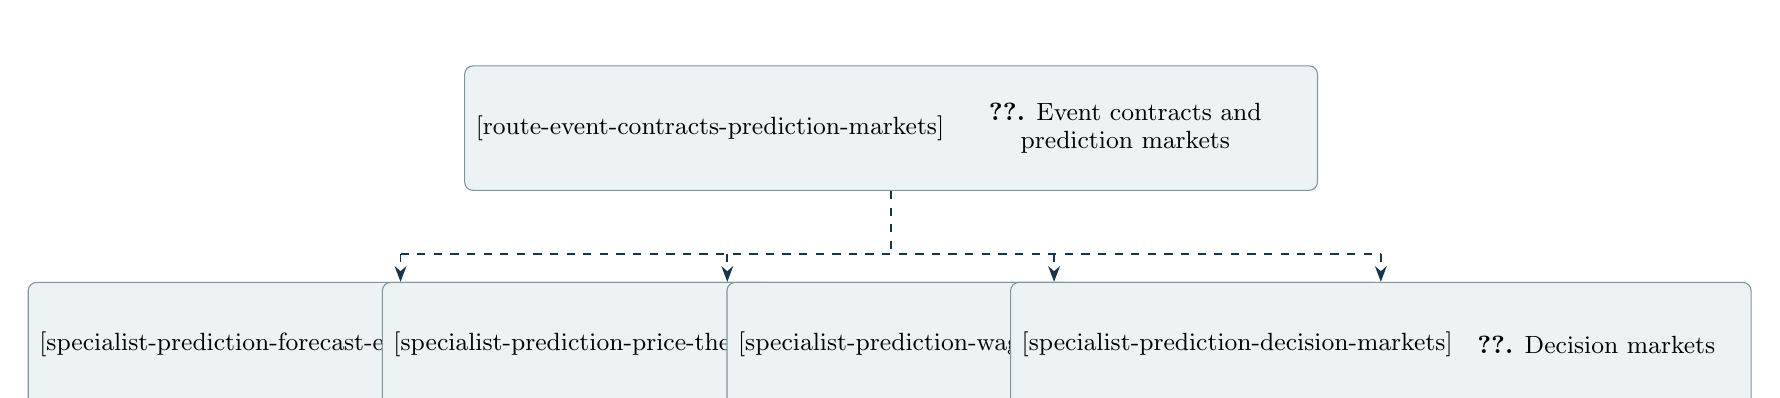
\begin{tikzpicture}[x=1cm,y=1cm]
\node[pathnode] (event-contracts-prediction-markets) at (6.23,0) {\MeasurePathNode{4.6cm}{\textbf{\ref*{route-event-contracts-prediction-markets}.} Event contracts and prediction markets}\hyperref[route-event-contracts-prediction-markets]{\parbox[c][\pathnodeheight][c]{4.6cm}{\centering \textbf{\ref*{route-event-contracts-prediction-markets}.} Event contracts and prediction markets}}};
\node[pathnode] (prediction-forecast-evidence) at (0.00,-2.75) {\MeasurePathNode{3.65cm}{\textbf{\ref*{specialist-prediction-forecast-evidence}.} Event prices as forecasts}\hyperref[specialist-prediction-forecast-evidence]{\parbox[c][\pathnodeheight][c]{3.65cm}{\centering \textbf{\ref*{specialist-prediction-forecast-evidence}.} Event prices as forecasts}}};
\node[pathnode] (prediction-price-theory) at (4.15,-2.75) {\MeasurePathNode{3.65cm}{\textbf{\ref*{specialist-prediction-price-theory}.} Beliefs and price theory}\hyperref[specialist-prediction-price-theory]{\parbox[c][\pathnodeheight][c]{3.65cm}{\centering \textbf{\ref*{specialist-prediction-price-theory}.} Beliefs and price theory}}};
\node[pathnode] (prediction-wagering) at (8.30,-2.75) {\MeasurePathNode{3.65cm}{\textbf{\ref*{specialist-prediction-wagering}.} Wagering and longshot bias}\hyperref[specialist-prediction-wagering]{\parbox[c][\pathnodeheight][c]{3.65cm}{\centering \textbf{\ref*{specialist-prediction-wagering}.} Wagering and longshot bias}}};
\node[pathnode] (prediction-decision-markets) at (12.45,-2.75) {\MeasurePathNode{3.65cm}{\textbf{\ref*{specialist-prediction-decision-markets}.} Decision markets}\hyperref[specialist-prediction-decision-markets]{\parbox[c][\pathnodeheight][c]{3.65cm}{\centering \textbf{\ref*{specialist-prediction-decision-markets}.} Decision markets}}};
\draw[entryline] (event-contracts-prediction-markets.south) -- (6.23,-1.60);
\draw[entryline] (0.00,-1.60) -- (12.45,-1.60);
\draw[entryarrow] (0.00,-1.60) -- (prediction-forecast-evidence.north);
\draw[entryarrow] (4.15,-1.60) -- (prediction-price-theory.north);
\draw[entryarrow] (8.30,-1.60) -- (prediction-wagering.north);
\draw[entryarrow] (12.45,-1.60) -- (prediction-decision-markets.north);
\end{tikzpicture}\end{center}
\textbf{Bring these foundations with you.}\begin{itemize}
\item \hyperref[route-empirical-causal-research]{Empirical asset pricing and causal inference} --- needed by \hyperref[specialist-prediction-forecast-evidence]{Event prices as forecasts}.
\end{itemize}\hyperref[learning-map]{Return to the whole-guide DAG.}
\Needspace{12\baselineskip}
\subsection{Event prices as forecasts: accuracy, calibration and bias}\label{specialist-prediction-forecast-evidence}
\textbf{Specialist pathway.} In \hyperref[route-event-contracts-prediction-markets]{Event contracts and prediction markets}.

\textbf{Outcome.} Measure whether event prices are calibrated and timely, explain the favourite–longshot pattern, and use price changes in event studies without overstating causality.

\textbf{Prerequisites.} Event contracts and prediction markets; regression and forecast calibration, and the Empirical asset pricing and causal inference overview for identification. Event studies and long-run abnormal returns (2.7) helps with the event-study readings.

\textbf{Review first.} \hyperref[route-event-contracts-prediction-markets]{Event contracts and prediction markets}; \hyperref[route-empirical-causal-research]{Empirical asset pricing and causal inference}.

\textbf{Required readings, in order}
\begin{enumerate}\raggedright
\Needspace{5\baselineskip}\item \href{institutional_quantitative_finance_reading_list.pdf\#pm-snowberg-wolfers-2010}{Erik Snowberg and Justin Wolfers, ``Explaining the Favorite--Long Shot Bias: Is it Risk-Love or Misperceptions?''}\CataloguePage{498}\NoteKey{pm-snowberg-wolfers-2010}\par \textbf{Evidence.} Separate a taste for risk from misperceived small probabilities as explanations of the favourite–longshot bias.
\Needspace{5\baselineskip}\item \href{institutional_quantitative_finance_reading_list.pdf\#pm-ottaviani-sorensen-2015}{Marco Ottaviani and Peter Norman Sørensen, ``Price Reaction to Information with Heterogeneous Beliefs and Wealth Effects: Underreaction, Momentum, and Reversal''}\CataloguePage{498}\NoteKey{pm-ottaviani-sorensen-2015}\par \textbf{Valuation.} See how belief dispersion and wealth effects make prices underreact to news, then drift.
\Needspace{5\baselineskip}\item \href{institutional_quantitative_finance_reading_list.pdf\#ev-rhode-strumpf-2004}{Paul W. Rhode and Koleman S. Strumpf, ``Historical Presidential Betting Markets''}\CataloguePage{500}\NoteKey{ev-rhode-strumpf-2004}\par \textbf{Evidence.} Start the election record in 1868: pre-poll betting markets, their accuracy and attempts to manipulate them.
\Needspace{5\baselineskip}\item \href{institutional_quantitative_finance_reading_list.pdf\#pm-berg-nelson-rietz-2008}{Joyce E. Berg, Forrest D. Nelson and Thomas A. Rietz, ``Prediction Market Accuracy in the Long Run''}\CataloguePage{498}\NoteKey{pm-berg-nelson-rietz-2008}\par \textbf{Evidence.} Compare long-run election-market forecasts with polls across five presidential elections.
\Needspace{5\baselineskip}\item \href{institutional_quantitative_finance_reading_list.pdf\#pm-erikson-wlezien-2008}{Robert S. Erikson and Christopher Wlezien, ``Are Political Markets Really Superior to Polls as Election Predictors?''}\CataloguePage{498}\NoteKey{pm-erikson-wlezien-2008}\par \textbf{Evidence.} Repeat the comparison after projecting polls to election day.
\Needspace{5\baselineskip}\item \href{institutional_quantitative_finance_reading_list.pdf\#pm-rothschild-2009}{David Rothschild, ``Forecasting Elections: Comparing Prediction Markets, Polls, and Their Biases''}\CataloguePage{498}\NoteKey{pm-rothschild-2009}\par \textbf{Evidence.} Debias both market prices and polls before scoring either.
\Needspace{5\baselineskip}\item \href{institutional_quantitative_finance_reading_list.pdf\#pm-page-clemen-2013}{Lionel Page and Robert T. Clemen, ``Do Prediction Markets Produce Well-Calibrated Probability Forecasts?''}\CataloguePage{499}\NoteKey{pm-page-clemen-2013}\par \textbf{Evidence.} Check calibration by horizon: the longshot bias is strongest far from resolution.
\Needspace{5\baselineskip}\item \href{institutional_quantitative_finance_reading_list.pdf\#pm-atanasov-2017}{Pavel Atanasov, Phillip Rescober, Eric Stone, Samuel A. Swift, Emile Servan-Schreiber, Philip Tetlock, Lyle Ungar and Barbara Mellers, ``Distilling the Wisdom of Crowds: Prediction Markets vs. Prediction Polls''}\CataloguePage{499}\NoteKey{pm-atanasov-2017}\par \textbf{Evidence.} Compare markets with aggregated team polls on identical questions under random assignment.
\Needspace{5\baselineskip}\item \href{institutional_quantitative_finance_reading_list.pdf\#ev-reichenbach-walther-2026}{Felix Reichenbach and Martin Walther, ``When Can Prediction Market Prices Be Trusted? Price Informativeness, Calibration, and Bias on Polymarket''}\CataloguePage{500}\NoteKey{ev-reichenbach-walther-2026}\par \textbf{Evidence.} Check when Polymarket prices can be trusted: by category, market age, activity and live trading.
\Needspace{5\baselineskip}\item \href{institutional_quantitative_finance_reading_list.pdf\#wide-le-prediction-calibration}{Author as listed on arXiv (Le), ``Decomposing Crowd Wisdom: Domain-Specific Calibration Dynamics in Prediction Markets''}\CataloguePage{499}\NoteKey{wide-le-prediction-calibration}\par \textbf{Evidence.} Break calibration down by domain, horizon and trade size on Kalshi and Polymarket; treat it as an associational preprint.
\Needspace{5\baselineskip}\item \href{institutional_quantitative_finance_reading_list.pdf\#pm-burgi-deng-whelan-2026}{Constantin Bürgi, Wanying Deng and Karl Whelan, ``Makers and Takers: The Economics of the Kalshi Prediction Market''}\CataloguePage{511}\NoteKey{pm-burgi-deng-whelan-2026}\par \textbf{Evidence.} Measure returns by price level and by maker or taker side on a regulated exchange.
\Needspace{5\baselineskip}\item \href{institutional_quantitative_finance_reading_list.pdf\#pm-gurkaynak-wolfers-2005}{Refet S. Gürkaynak and Justin Wolfers, ``Macroeconomic Derivatives: An Initial Analysis of Market-Based Macro Forecasts, Uncertainty, and Risk''; NBER working paper}\CataloguePage{512}\NoteKey{pm-gurkaynak-wolfers-2005}\par \textbf{Evidence.} Assess market forecasts of macro data releases against the survey consensus, including the implied distribution.
\Needspace{5\baselineskip}\item \href{institutional_quantitative_finance_reading_list.pdf\#catalogue-0883}{Anthony M. Diercks, Jared Dean Katz and Jonathan H. Wright, ``Kalshi and the Rise of Macro Markets''; Federal Reserve FEDS version}\CataloguePage{499}\NoteKey{catalogue-0883}\par \textbf{Evidence.} Benchmark current macro and policy-rate event markets against surveys and futures-implied expectations.
\Needspace{5\baselineskip}\item \href{institutional_quantitative_finance_reading_list.pdf\#catalogue-0882}{Mikhail Chernov, Vadim Elenev and Dongho Song, ``The Comovement of Voter Preferences: Insights from U.S. Presidential Election Prediction Markets Beyond Polls''; journal version}\CataloguePage{499}\NoteKey{catalogue-0882}\par \textbf{Evidence.} Model correlated outcomes across states rather than treating each contract as independent.
\Needspace{5\baselineskip}\item \href{institutional_quantitative_finance_reading_list.pdf\#pm-snowberg-wolfers-zitzewitz-2007}{Erik Snowberg, Justin Wolfers and Eric Zitzewitz, ``Partisan Impacts on the Economy: Evidence from Prediction Markets and Close Elections''}\CataloguePage{499}\NoteKey{pm-snowberg-wolfers-zitzewitz-2007}\par \textbf{Event study.} Scale high-frequency asset-price moves by the change in an event probability.
\Needspace{5\baselineskip}\item \href{institutional_quantitative_finance_reading_list.pdf\#wide-gneiting-raftery}{Tilmann Gneiting and Adrian E. Raftery, ``Strictly Proper Scoring Rules, Prediction, and Estimation''}\CataloguePage{39}\NoteKey{wide-gneiting-raftery}\par \textbf{Validation.} Score probability forecasts with proper scoring rules before claiming one source beats another.
\end{enumerate}
\Needspace{5\baselineskip}\textbf{Checkpoint.} Collect resolved contracts in one category from two venues. Bin them by price and horizon, plot realised frequency against price with confidence bands, and compute returns by price bin net of fees, by maker and taker side where fills allow. Score the prices against a poll- or model-based forecast for the same events with Brier and log scores, clustering by event date, and report which differences survive.

\textbf{Optional branches.} \href{institutional_quantitative_finance_reading_list.pdf\#pm-moskowitz-2021}{Test momentum and value in sports-betting lines, where contracts carry no systematic risk.}\BranchPage{513} \href{institutional_quantitative_finance_reading_list.pdf\#pm-croxson-reade-2014}{Measure how quickly prices absorb news, using goals just before half-time.}\BranchPage{499} \href{institutional_quantitative_finance_reading_list.pdf\#ev-lee-lee-lee-2026-sports}{Measure how fast in-play sports prices absorb scoring news, and whether the lag pays after costs.}\BranchPage{500}
\par{\small \hyperref[learning-map]{Learning pathway DAG} \textbar{} \hyperref[route-event-contracts-prediction-markets]{Section overview} \textbar{} \hyperref[map-event-contracts-prediction-markets]{Section DAG}\NoteKey{prediction-forecast-evidence}}
\Needspace{12\baselineskip}
\subsection{Price theory: beliefs, wealth and belief dynamics}\label{specialist-prediction-price-theory}
\textbf{Specialist pathway.} In \hyperref[route-event-contracts-prediction-markets]{Event contracts and prediction markets}.

\textbf{Outcome.} Derive when an event price equals the mean belief and when it does not, test whether a price path moves like a rational probability, and explain why informed trading does or does not reveal information.

\textbf{Prerequisites.} Event contracts and prediction markets; expected utility, competitive equilibrium and martingales from the Common toolkit.

\textbf{Review first.} \hyperref[route-event-contracts-prediction-markets]{Event contracts and prediction markets}.

\textbf{Required readings, in order}
\begin{enumerate}\raggedright
\Needspace{5\baselineskip}\item \href{institutional_quantitative_finance_reading_list.pdf\#ev-he-treich-2017}{Xue-Zhong He and Nicolas Treich, ``Prediction market prices under risk aversion and heterogeneous beliefs''}\CataloguePage{498}\NoteKey{ev-he-treich-2017}\par \textbf{Theory.} Prove when prices equal mean beliefs (log utility only) and when they sit above or below them.
\Needspace{5\baselineskip}\item \href{institutional_quantitative_finance_reading_list.pdf\#pm-ottaviani-sorensen-2015}{Marco Ottaviani and Peter Norman Sørensen, ``Price Reaction to Information with Heterogeneous Beliefs and Wealth Effects: Underreaction, Momentum, and Reversal''}\CataloguePage{498}\NoteKey{pm-ottaviani-sorensen-2015}\par \textbf{Theory.} Add wealth effects: why prices underreact to news when beliefs are dispersed.
\Needspace{5\baselineskip}\item \href{institutional_quantitative_finance_reading_list.pdf\#pm-ostrovsky-2012}{Michael Ostrovsky, ``Information Aggregation in Dynamic Markets With Strategic Traders''}\CataloguePage{497}\NoteKey{pm-ostrovsky-2012}\par \textbf{Theory.} Identify which securities aggregate dispersed information when informed traders act strategically.
\Needspace{5\baselineskip}\item \href{institutional_quantitative_finance_reading_list.pdf\#ev-page-siemroth-2017}{Lionel Page and Christoph Siemroth, ``An experimental analysis of information acquisition in prediction markets''}\CataloguePage{504}\NoteKey{ev-page-siemroth-2017}\par \textbf{Evidence.} See in the laboratory that traders overbuy information, which pushes prices towards fundamentals.
\Needspace{5\baselineskip}\item \href{institutional_quantitative_finance_reading_list.pdf\#ev-gao-wang-wu-yu-2025}{Jianjun Gao, Zizhuo Wang, Weiping Wu and Dian Yu, ``Price Interpretability of Prediction Markets: A Convergence Analysis''}\CataloguePage{510}\NoteKey{ev-gao-wang-wu-yu-2025}\par \textbf{Theory.} Follow the limiting price when risk-averse traders with different beliefs trade repeatedly with a market maker.
\Needspace{5\baselineskip}\item \href{institutional_quantitative_finance_reading_list.pdf\#ev-augenblick-rabin-2021}{Ned Augenblick and Matthew Rabin, ``Belief Movement, Uncertainty Reduction, and Rational Updating''}\CataloguePage{498}\NoteKey{ev-augenblick-rabin-2021}\par \textbf{Methods.} Test whether a price path moves too much or too little for a Bayesian probability.
\end{enumerate}
\Needspace{5\baselineskip}\textbf{Checkpoint.} Solve a two-state market with CRRA traders whose beliefs and wealth differ, and plot the equilibrium price against the wealth-weighted and simple mean beliefs as risk aversion varies. Then take the price paths of fifty resolved contracts, compute belief movement and uncertainty reduction, and test whether they are equal on average; report which contracts show excess movement.

\textbf{Optional branches.} \href{institutional_quantitative_finance_reading_list.pdf\#catalogue-0880}{Return to the bounds on mean beliefs implied by a price when traders are risk neutral.}\BranchPage{497} \href{institutional_quantitative_finance_reading_list.pdf\#ev-archak-ipeirotis-2009}{Model the volatility of a rational event price as a function of price and time to expiry.}\BranchPage{513}
\par{\small \hyperref[learning-map]{Learning pathway DAG} \textbar{} \hyperref[route-event-contracts-prediction-markets]{Section overview} \textbar{} \hyperref[map-event-contracts-prediction-markets]{Section DAG}\NoteKey{prediction-price-theory}}
\Needspace{12\baselineskip}
\subsection{Wagering markets: bookmakers, exchanges and the favourite–longshot bias}\label{specialist-prediction-wagering}
\textbf{Specialist pathway.} In \hyperref[route-event-contracts-prediction-markets]{Event contracts and prediction markets}.

\textbf{Outcome.} Explain the favourite–longshot bias with risk preferences, misperception, private information or dealer pricing, and show how market structure (parimutuel pool, bookmaker or exchange) changes calibration.

\textbf{Prerequisites.} Event contracts and prediction markets; maximum-likelihood estimation and expected utility.

\textbf{Review first.} \hyperref[route-event-contracts-prediction-markets]{Event contracts and prediction markets}.

\textbf{Required readings, in order}
\begin{enumerate}\raggedright
\Needspace{5\baselineskip}\item \href{institutional_quantitative_finance_reading_list.pdf\#ev-ali-1977}{Mukhtar M. Ali, ``Probability and Utility Estimates for Racetrack Bettors''}\CataloguePage{500}\NoteKey{ev-ali-1977}\par \textbf{Evidence.} Back a bettor's utility out of 20,000 races: longshots overbet, favourites underbet.
\Needspace{5\baselineskip}\item \href{institutional_quantitative_finance_reading_list.pdf\#pm-snowberg-wolfers-2010}{Erik Snowberg and Justin Wolfers, ``Explaining the Favorite--Long Shot Bias: Is it Risk-Love or Misperceptions?''}\CataloguePage{498}\NoteKey{pm-snowberg-wolfers-2010}\par \textbf{Evidence.} Separate risk-love from misperceived probabilities with exotic bets.
\Needspace{5\baselineskip}\item \href{institutional_quantitative_finance_reading_list.pdf\#ev-jullien-salanie-2000}{Bruno Jullien and Bernard Salanié, ``Estimating Preferences under Risk: The Case of Racetrack Bettors''}\CataloguePage{500}\NoteKey{ev-jullien-salanie-2000}\par \textbf{Evidence.} Estimate non-expected-utility preferences from 34,000 British races.
\Needspace{5\baselineskip}\item \href{institutional_quantitative_finance_reading_list.pdf\#ev-ottaviani-sorensen-2009}{Marco Ottaviani and Peter Norman Sørensen, ``Surprised by the Parimutuel Odds?''}\CataloguePage{502}\NoteKey{ev-ottaviani-sorensen-2009}\par \textbf{Theory.} See how private information and simultaneous betting create the bias in a parimutuel pool.
\Needspace{5\baselineskip}\item \href{institutional_quantitative_finance_reading_list.pdf\#ev-ottaviani-sorensen-2010}{Marco Ottaviani and Peter Norman Sørensen, ``Noise, Information, and the Favorite--Longshot Bias in Parimutuel Predictions''}\CataloguePage{502}\NoteKey{ev-ottaviani-sorensen-2010}\par \textbf{Theory.} Turn the information-to-noise ratio into testable predictions about the bias.
\Needspace{5\baselineskip}\item \href{institutional_quantitative_finance_reading_list.pdf\#ev-shin-1991}{Hyun Song Shin, ``Optimal Betting Odds Against Insider Traders''}\CataloguePage{506}\NoteKey{ev-shin-1991}\par \textbf{Theory.} Derive the bookmaker's square-root pricing rule against insiders.
\Needspace{5\baselineskip}\item \href{institutional_quantitative_finance_reading_list.pdf\#ev-levitt-2004}{Steven D. Levitt, ``Why are Gambling Markets Organised so Differently from Financial Markets?''}\CataloguePage{501}\NoteKey{ev-levitt-2004}\par \textbf{Evidence.} See why bookmakers take positions instead of matching orders, and what it earns them.
\Needspace{5\baselineskip}\item \href{institutional_quantitative_finance_reading_list.pdf\#ev-whelan-2024-flb}{Karl Whelan, ``Risk Aversion and Favourite--Longshot Bias in a Competitive Fixed-Odds Betting Market''}\CataloguePage{502}\NoteKey{ev-whelan-2024-flb}\par \textbf{Theory.} Explain the bias in competitive fixed-odds markets with bettor disagreement and bookmaker risk aversion.
\Needspace{5\baselineskip}\item \href{institutional_quantitative_finance_reading_list.pdf\#ev-smith-paton-williams-2006}{Michael A. Smith, David Paton and Leighton Vaughan Williams, ``Market Efficiency in Person‐to‐Person Betting''}\CataloguePage{501}\NoteKey{ev-smith-paton-williams-2006}\par \textbf{Evidence.} Compare betting exchanges with bookmakers on matched races.
\Needspace{5\baselineskip}\item \href{institutional_quantitative_finance_reading_list.pdf\#ev-hegarty-whelan-2025}{Tadgh Hegarty and Karl Whelan, ``Forecasting soccer matches with betting odds: A tale of two markets''}\CataloguePage{501}\NoteKey{ev-hegarty-whelan-2025}\par \textbf{Evidence.} Contrast a biased 1X2 market with an efficient Asian-handicap market on the same matches.
\Needspace{5\baselineskip}\item \href{institutional_quantitative_finance_reading_list.pdf\#ev-woodland-woodland-1994}{Linda M. Woodland and Bill M. Woodland, ``Market Efficiency and the Favorite--Longshot Bias: The Baseball Betting Market''}\CataloguePage{501}\NoteKey{ev-woodland-woodland-1994}\par \textbf{Counter-evidence.} Find the bias reversed in baseball, and unprofitable after commissions.
\Needspace{5\baselineskip}\item \href{institutional_quantitative_finance_reading_list.pdf\#ev-meyer-hundtofte-2023}{Andrew Meyer and Sean Hundtofte, ``The Longshot Bias Is a Context Effect''}\CataloguePage{502}\NoteKey{ev-meyer-hundtofte-2023}\par \textbf{Evidence.} Test a presentation-based explanation: contrasts between payoffs make longshots attractive.
\Needspace{5\baselineskip}\item \href{institutional_quantitative_finance_reading_list.pdf\#ev-newall-cortis-2021}{Philip W. S. Newall and Dominic Cortis, ``Are Sports Bettors Biased toward Longshots, Favorites, or Both? A Literature Review''}\CataloguePage{502}\NoteKey{ev-newall-cortis-2021}\par \textbf{Evidence.} Reconcile longshot and favourite biases by the number of outcomes and odds range.
\end{enumerate}
\Needspace{5\baselineskip}\textbf{Checkpoint.} Collect closing odds or prices for one sport from a bookmaker and an exchange (or Kalshi and Polymarket) over at least two seasons. Remove the margin by proportional scaling and by Shin's method, bin by implied probability and plot realised win rates with confidence bands. Fit a risk-preference model and an information model to the same data and report which explains the pattern, and whether the exchange shows a smaller bias.

\textbf{Optional branches.} \href{institutional_quantitative_finance_reading_list.pdf\#ev-vaughan-williams-1999}{Survey the older efficiency literature by form of efficiency.}\BranchPage{501} \href{institutional_quantitative_finance_reading_list.pdf\#ev-franck-verbeek-nuesch-2010}{Compare exchange and bookmaker accuracy on 5,478 football matches.}\BranchPage{501} \href{institutional_quantitative_finance_reading_list.pdf\#ev-elaad-reade-singleton-2020}{Test whether bookmakers use competitors' odds efficiently.}\BranchPage{501} \href{institutional_quantitative_finance_reading_list.pdf\#ev-casadesus-masanell-campbell-2019}{Follow how Betfair entered and then coexisted with bookmakers.}\BranchPage{501}
\par{\small \hyperref[learning-map]{Learning pathway DAG} \textbar{} \hyperref[route-event-contracts-prediction-markets]{Section overview} \textbar{} \hyperref[map-event-contracts-prediction-markets]{Section DAG}\NoteKey{prediction-wagering}}
\Needspace{12\baselineskip}
\subsection{Decision, corporate and scientific markets}\label{specialist-prediction-decision-markets}
\textbf{Specialist pathway.} In \hyperref[route-event-contracts-prediction-markets]{Event contracts and prediction markets}.

\textbf{Outcome.} Design a market whose price informs a decision, keeping incentives intact when only the chosen action is scored, and judge whether a market beats a cheaper poll or model.

\textbf{Prerequisites.} Event contracts and prediction markets; proper scoring rules and basic mechanism design.

\textbf{Review first.} \hyperref[route-event-contracts-prediction-markets]{Event contracts and prediction markets}.

\textbf{Required readings, in order}
\begin{enumerate}\raggedright
\Needspace{5\baselineskip}\item \href{institutional_quantitative_finance_reading_list.pdf\#ev-hanson-2013-futarchy}{Robin Hanson, ``Shall We Vote on Values, But Bet on Beliefs?''}\CataloguePage{503}\NoteKey{ev-hanson-2013-futarchy}\par \textbf{Mechanics.} Read the proposal to price welfare conditional on a policy and adopt what the market favours.
\Needspace{5\baselineskip}\item \href{institutional_quantitative_finance_reading_list.pdf\#ev-chen-kash-ruberry-shnayder-2011}{Yiling Chen, Ian Kash, Mike Ruberry and Victor Shnayder, ``Decision Markets with Good Incentives''}\CataloguePage{503}\NoteKey{ev-chen-kash-ruberry-shnayder-2011}\par \textbf{Theory.} See why decision markets break scoring-rule incentives, and the randomisation that restores them.
\Needspace{5\baselineskip}\item \href{institutional_quantitative_finance_reading_list.pdf\#ev-spann-skiera-2003}{Martin Spann and Bernd Skiera, ``Internet-Based Virtual Stock Markets for Business Forecasting''}\CataloguePage{503}\NoteKey{ev-spann-skiera-2003}\par \textbf{Evidence.} Run virtual stock markets for business forecasts and compare them with experts.
\Needspace{5\baselineskip}\item \href{institutional_quantitative_finance_reading_list.pdf\#pm-cowgill-zitzewitz-2015}{Bo Cowgill and Eric Zitzewitz, ``Corporate Prediction Markets: Evidence from Google, Ford, and Firm X''}\CataloguePage{502}\NoteKey{pm-cowgill-zitzewitz-2015}\par \textbf{Evidence.} Measure the biases in corporate markets at Google, Ford and a third firm.
\Needspace{5\baselineskip}\item \href{institutional_quantitative_finance_reading_list.pdf\#ev-gillen-plott-shum-2017}{Benjamin J. Gillen, Charles R. Plott and Matthew Shum, ``A Pari-Mutuel-Like Mechanism for Information Aggregation: A Field Test inside Intel''}\CataloguePage{503}\NoteKey{ev-gillen-plott-shum-2017}\par \textbf{Evidence.} Follow a pari-mutuel-like mechanism forecasting sales inside Intel.
\Needspace{5\baselineskip}\item \href{institutional_quantitative_finance_reading_list.pdf\#ev-servan-schreiber-2004}{Emile Servan-Schreiber, Justin Wolfers, David M. Pennock and Brian Galebach, ``Prediction Markets: Does Money Matter?''}\CataloguePage{503}\NoteKey{ev-servan-schreiber-2004}\par \textbf{Evidence.} Test whether real money beats play money.
\Needspace{5\baselineskip}\item \href{institutional_quantitative_finance_reading_list.pdf\#ev-dreber-2015}{Anna Dreber, Thomas Pfeiffer, Johan Almenberg, Siri Isaksson, Brad Wilson, Yiling Chen, Brian A. Nosek and Magnus Johannesson, ``Using prediction markets to estimate the reproducibility of scientific research''}\CataloguePage{503}\NoteKey{ev-dreber-2015}\par \textbf{Evidence.} Use markets to predict which studies replicate.
\Needspace{5\baselineskip}\item \href{institutional_quantitative_finance_reading_list.pdf\#ev-goel-reeves-watts-pennock-2010}{Sharad Goel, Daniel M. Reeves, Duncan J. Watts and David M. Pennock, ``Prediction without markets''}\CataloguePage{503}\NoteKey{ev-goel-reeves-watts-pennock-2010}\par \textbf{Counter-evidence.} Check how small the market advantage over polls and models can be.
\end{enumerate}
\Needspace{5\baselineskip}\textbf{Checkpoint.} Design a conditional market for a decision you know (a product launch or a hiring choice): write the contracts, the scoring or payout rule and what happens to trades on the action not taken. Show with a two-action example how an expert could profit by misleading the decision maker under a naive design, then fix it with the randomised rule. Finally compare the market forecast with a poll and a two-parameter model on past cases, using Brier scores.

\textbf{Optional branches.} \href{institutional_quantitative_finance_reading_list.pdf\#pm-atanasov-2017}{Compare markets with aggregated team polls under random assignment.}\BranchPage{499} \href{institutional_quantitative_finance_reading_list.pdf\#ev-arrow-2008}{Read the economists' case for legal research and corporate markets.}\BranchPage{502}
\par{\small \hyperref[learning-map]{Learning pathway DAG} \textbar{} \hyperref[route-event-contracts-prediction-markets]{Section overview} \textbar{} \hyperref[map-event-contracts-prediction-markets]{Section DAG}\NoteKey{prediction-decision-markets}}
\clearpage
\section{Event-contract venues, settlement and regulation}\label{route-event-contract-venues}
\label{route-37}
\textbf{Learning sequence.} Four independent pathways: resolution and settlement data; outcome tokens, fractional contracts and cross-venue identity; insider trading, manipulation and wash trading; and regulation and litigation. Read the settlement pathway before using any realised-return data.

\textbf{Section goals.} Across its pathways, this section teaches you to:
\begin{itemize}[leftmargin=1.4em,itemsep=0pt,topsep=1pt]
\item interpret prices only after resolution, dispute, payout and cash-release terms are explicit (\hyperref[specialist-prediction-settlement]{\ref*{specialist-prediction-settlement}})
\item represent event claims as tokens or exchange positions and match listings across venues (\hyperref[specialist-prediction-outcome-tokens]{\ref*{specialist-prediction-outcome-tokens}})
\item screen trade records for insider trading, manipulation and wash trading (\hyperref[specialist-prediction-integrity]{\ref*{specialist-prediction-integrity}})
\item state which authority governs a contract and what pending cases could change (\hyperref[specialist-prediction-regulation]{\ref*{specialist-prediction-regulation}})
\end{itemize}
\textbf{Overview outcome.} Before using a price or volume series, state who lists the contract and under what licence, how a position is held and redeemed, who determines the outcome and how it can be disputed, and what the trade record may hide.

\textbf{Prerequisites.} Event contracts and prediction markets (Section 36); binary-option payoffs and basic market microstructure. Tokenised and fractional assets (Section 33) helps with on-chain venues but is not required.

\textbf{Review first.} \hyperref[route-event-contracts-prediction-markets]{Event contracts and prediction markets}.

\textbf{Required readings, in order}
\begin{enumerate}\raggedright
\Needspace{5\baselineskip}\item \href{institutional_quantitative_finance_reading_list.pdf\#pm-crs-policy-2026}{Karl E. Schneider and Rena S. Miller, Congressional Research Service, ``Prediction Markets: Policy Issues for Congress'' (In Focus IF13187)}\CataloguePage{508}\NoteKey{pm-crs-policy-2026}\par Map the current venues, contract categories and open regulatory questions.
\Needspace{5\baselineskip}\item \href{institutional_quantitative_finance_reading_list.pdf\#ev-casadesus-masanell-campbell-2019}{Ramon Casadesus-Masanell and Neil Campbell, ``Platform competition: Betfair and the UK market for sports betting''}\CataloguePage{501}\NoteKey{ev-casadesus-masanell-campbell-2019}\par See how an exchange entered a market of bookmakers and came to coexist with them.
\Needspace{5\baselineskip}\item \href{institutional_quantitative_finance_reading_list.pdf\#ev-polymarket-positions}{Polymarket, How Positions Work; Negative Risk Markets; Combinatorial Positions}\CataloguePage{506}\NoteKey{ev-polymarket-positions}\par Learn how an on-chain position is minted, merged, converted and redeemed as fractional, collateralised tokens.
\Needspace{5\baselineskip}\item \href{institutional_quantitative_finance_reading_list.pdf\#add-prediction-settlement}{Kalshi, Market FAQs}\CataloguePage{504}\NoteKey{add-prediction-settlement}\par Compare an exchange's settlement and cash-release rules.
\Needspace{5\baselineskip}\item \href{institutional_quantitative_finance_reading_list.pdf\#ev-polymarket-resolution}{Polymarket, Resolution}\CataloguePage{505}\NoteKey{ev-polymarket-resolution}\par Read how an on-chain venue resolves markets through an optimistic oracle, and why the rules, not the title, define the payoff.
\Needspace{5\baselineskip}\item \href{institutional_quantitative_finance_reading_list.pdf\#ev-cftc-polymarket-2022}{U.S. Commodity Futures Trading Commission, CFTC Orders Event-Based Binary Options Markets Operator to Pay \$1.4 Million Penalty (Release 8478-22)}\CataloguePage{508}\NoteKey{ev-cftc-polymarket-2022}\par See why an on-chain event market was still a derivatives venue under U.S. law.
\end{enumerate}
\Needspace{5\baselineskip}\textbf{Checkpoint.} Pick one event listed on a regulated exchange and on an on-chain venue. For each, record the legal wrapper, the position (contract, token identifier, fractional size and tick), the resolution source and dispute route, the settlement and cash-release timing, and the fees. List every way the two contracts could pay differently on the same real-world outcome, and say which price you would treat as the forecast.

\textbf{Optional branches.} \href{institutional_quantitative_finance_reading_list.pdf\#w2-crs-cftc-prediction}{Track the 2026 CFTC event-contract proposal and the split over sports contracts.}\BranchPage{508} \href{institutional_quantitative_finance_reading_list.pdf\#ev-gebele-matthes-2026-lop}{Measure how often the same event is listed on several venues and how far prices diverge.}\BranchPage{505}
\par\textbf{Continue in this section.} \hyperref[specialist-prediction-settlement]{Contract resolution, disputes and settlement data}; \hyperref[specialist-prediction-outcome-tokens]{Outcome tokens, fractional contracts and cross-venue identity}; \hyperref[specialist-prediction-integrity]{Insider trading, manipulation and wash trading}; \hyperref[specialist-prediction-regulation]{Regulation and litigation: the CFTC, states and sports contracts}.
\par{\small \hyperref[learning-map]{Learning pathway DAG} \textbar{} \hyperref[map-event-contract-venues]{Section DAG}\NoteKey{event-contract-venues}}
\clearpage
\subsection*{Event-contract venues, settlement and regulation: pathway DAG}\phantomsection\label{map-event-contract-venues}
\addcontentsline{toc}{subsection}{Event-contract venues, settlement and regulation: pathway DAG}
Start with the section overview's readings, for orientation. Solid arrows show prerequisites within this section. Dashed connectors identify entry points with no further prerequisite in this section; the linked foundations below still apply. Follow the arrows for dependencies and the subsection numbers for reading order. Every node is clickable.
\begin{center}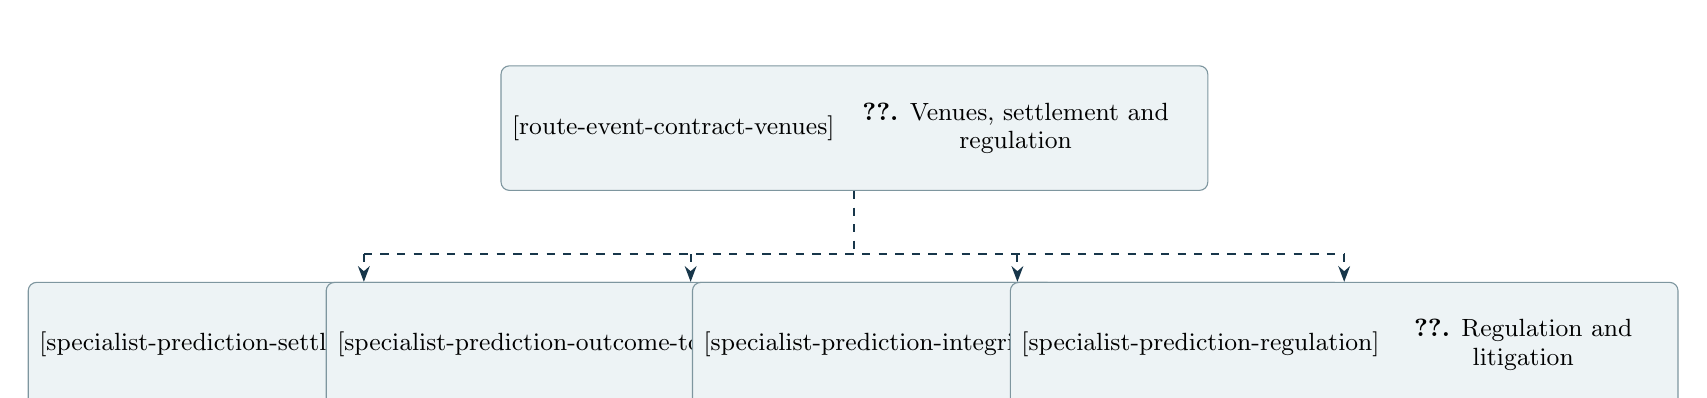
\begin{tikzpicture}[x=1cm,y=1cm]
\node[pathnode] (event-contract-venues) at (6.23,0) {\MeasurePathNode{4.6cm}{\textbf{\ref*{route-event-contract-venues}.} Venues, settlement and regulation}\hyperref[route-event-contract-venues]{\parbox[c][\pathnodeheight][c]{4.6cm}{\centering \textbf{\ref*{route-event-contract-venues}.} Venues, settlement and regulation}}};
\node[pathnode] (prediction-settlement) at (0.00,-2.75) {\MeasurePathNode{3.65cm}{\textbf{\ref*{specialist-prediction-settlement}.} Resolution and settlement}\hyperref[specialist-prediction-settlement]{\parbox[c][\pathnodeheight][c]{3.65cm}{\centering \textbf{\ref*{specialist-prediction-settlement}.} Resolution and settlement}}};
\node[pathnode] (prediction-outcome-tokens) at (4.15,-2.75) {\MeasurePathNode{3.65cm}{\textbf{\ref*{specialist-prediction-outcome-tokens}.} Outcome tokens}\hyperref[specialist-prediction-outcome-tokens]{\parbox[c][\pathnodeheight][c]{3.65cm}{\centering \textbf{\ref*{specialist-prediction-outcome-tokens}.} Outcome tokens}}};
\node[pathnode] (prediction-integrity) at (8.30,-2.75) {\MeasurePathNode{3.65cm}{\textbf{\ref*{specialist-prediction-integrity}.} Integrity and manipulation}\hyperref[specialist-prediction-integrity]{\parbox[c][\pathnodeheight][c]{3.65cm}{\centering \textbf{\ref*{specialist-prediction-integrity}.} Integrity and manipulation}}};
\node[pathnode] (prediction-regulation) at (12.45,-2.75) {\MeasurePathNode{3.65cm}{\textbf{\ref*{specialist-prediction-regulation}.} Regulation and litigation}\hyperref[specialist-prediction-regulation]{\parbox[c][\pathnodeheight][c]{3.65cm}{\centering \textbf{\ref*{specialist-prediction-regulation}.} Regulation and litigation}}};
\draw[entryline] (event-contract-venues.south) -- (6.23,-1.60);
\draw[entryline] (0.00,-1.60) -- (12.45,-1.60);
\draw[entryarrow] (0.00,-1.60) -- (prediction-settlement.north);
\draw[entryarrow] (4.15,-1.60) -- (prediction-outcome-tokens.north);
\draw[entryarrow] (8.30,-1.60) -- (prediction-integrity.north);
\draw[entryarrow] (12.45,-1.60) -- (prediction-regulation.north);
\end{tikzpicture}\end{center}
\hyperref[learning-map]{Return to the whole-guide DAG.}
\Needspace{12\baselineskip}
\subsection{Contract resolution, disputes and settlement data}\label{specialist-prediction-settlement}
\textbf{Specialist pathway.} In \hyperref[route-event-contract-venues]{Event-contract venues, settlement and regulation}.

\textbf{Outcome.} Interpret event prices and returns only after the resolution, dispute, payout and cash-release terms are explicit, and build a market archive that keeps price, determination and redemption records apart.

\textbf{Prerequisites.} Event-contract venues, settlement and regulation; binary options and basic market microstructure.

\textbf{Review first.} \hyperref[route-event-contract-venues]{Event-contract venues, settlement and regulation}.

\textbf{Required readings, in order}
\begin{enumerate}\raggedright
\Needspace{5\baselineskip}\item \href{institutional_quantitative_finance_reading_list.pdf\#gapclose-kalshi-history}{Kalshi, Historical Market Data}\CataloguePage{504}\NoteKey{gapclose-kalshi-history}\par \textbf{Data.} Build the market archive across live and historical cutoffs while keeping account cash evidence separate.
\Needspace{5\baselineskip}\item \href{institutional_quantitative_finance_reading_list.pdf\#ev-kalshi-settlement-docs}{Kalshi, Market Settlement; Market Settlement}\CataloguePage{505}\NoteKey{ev-kalshi-settlement-docs}\par \textbf{Mechanics.} Read when a net position pays, and how a settlement floor would release collateral early on scalar markets.
\Needspace{5\baselineskip}\item \href{institutional_quantitative_finance_reading_list.pdf\#add-prediction-disputes}{Polymarket, How Are Markets Disputed?}\CataloguePage{504}\NoteKey{add-prediction-disputes}\par \textbf{Mechanics.} Read the on-chain venue's oracle proposal and challenge windows.
\Needspace{5\baselineskip}\item \href{institutional_quantitative_finance_reading_list.pdf\#ev-uma-optimistic-oracle}{UMA, How Does UMA Work? (Optimistic Oracle and Data Verification Mechanism)}\CataloguePage{505}\NoteKey{ev-uma-optimistic-oracle}\par \textbf{Mechanics.} Follow a request through proposal, bond, challenge window and token-holder vote.
\Needspace{5\baselineskip}\item \href{institutional_quantitative_finance_reading_list.pdf\#ev-williams-peterson-2019}{Austin K. Williams and Jack Peterson, ``Decentralized Common Knowledge Oracles''}\CataloguePage{505}\NoteKey{ev-williams-peterson-2019}\par \textbf{Theory.} See when reporters paid to state a common-knowledge outcome tell the truth.
\Needspace{5\baselineskip}\item \href{institutional_quantitative_finance_reading_list.pdf\#gapclose-polymarket-data}{Polymarket, Market Data, Data API v1 to v2 migration and Resolution; Polymarket market making; Polymarket positions and tokens; Polymarket negative-risk markets}\CataloguePage{504}\NoteKey{gapclose-polymarket-data}\par \textbf{Data and implementation.} Join outcome tokens, historical API schemas and redemption states before calculating realised event-contract returns.
\Needspace{5\baselineskip}\item \href{institutional_quantitative_finance_reading_list.pdf\#s11-r11}{Dune documentation; The Graph subgraphs; Glassnode Studio (documentation)}\CataloguePage{476}\NoteKey{s11-r11}\par \textbf{Data.} Audit on-chain state and payout timing for the on-chain venue.
\end{enumerate}
\Needspace{5\baselineskip}\textbf{Checkpoint.} Select one resolved contract on each venue. Archive the exact rules, resolution source, outcome-token identifiers and API version. Use Kalshi historical cutoffs and Polymarket cursor pagination to collect the available market observations. Record close, determination, proposal and any dispute, redemption and eventual cash conversion separately, with timestamps. Compute a scenario return after spread, fees and capital lock-up; claim realised P\&L only with matching fills, redemption or payment records and token conversion evidence.

\textbf{Optional branches.} \href{institutional_quantitative_finance_reading_list.pdf\#section.18.10}{For an on-chain venue, inspect contract permissions and failure modes before live exposure.}\BranchPage{493} \href{institutional_quantitative_finance_reading_list.pdf\#ev-peterson-augur-2015}{Compare a reputation-token oracle that forks when a dispute escalates.}\BranchPage{505}
\par{\small \hyperref[learning-map]{Learning pathway DAG} \textbar{} \hyperref[route-event-contract-venues]{Section overview} \textbar{} \hyperref[map-event-contract-venues]{Section DAG}\NoteKey{prediction-settlement}}
\Needspace{12\baselineskip}
\subsection{Outcome tokens, fractional contracts and cross-venue identity}\label{specialist-prediction-outcome-tokens}
\textbf{Specialist pathway.} In \hyperref[route-event-contract-venues]{Event-contract venues, settlement and regulation}.

\textbf{Outcome.} Represent an event claim as a fractional, fully collateralised token or exchange position, use split, merge and conversion operations correctly, and decide when two listings are the same asset.

\textbf{Prerequisites.} Event-contract venues, settlement and regulation; token standards and wallet transactions from Tokenised and fractional assets (Section 33) help but are not required.

\textbf{Review first.} \hyperref[route-event-contract-venues]{Event-contract venues, settlement and regulation}.

\textbf{Required readings, in order}
\begin{enumerate}\raggedright
\Needspace{5\baselineskip}\item \href{institutional_quantitative_finance_reading_list.pdf\#ev-gnosis-conditional-tokens}{Gnosis, Conditional Tokens Contracts (documentation, version 1.0.3)}\CataloguePage{505}\NoteKey{ev-gnosis-conditional-tokens}\par \textbf{Mechanics.} Learn the conditional-token framework: conditions, positions, split, merge and redeem, and nested conditions.
\Needspace{5\baselineskip}\item \href{institutional_quantitative_finance_reading_list.pdf\#ev-peterson-augur-2015}{Jack Peterson, Joseph Krug, Micah Zoltu, Austin K. Williams and Stephanie Alexander, ``Augur: A Decentralized Oracle and Prediction Market Platform''}\CataloguePage{505}\NoteKey{ev-peterson-augur-2015}\par \textbf{Mechanics.} Compare an earlier on-chain design whose reputation token underwrites settlement.
\Needspace{5\baselineskip}\item \href{institutional_quantitative_finance_reading_list.pdf\#ev-kalshi-fixed-point}{Kalshi, Fixed-Point Representation}\CataloguePage{506}\NoteKey{ev-kalshi-fixed-point}\par \textbf{Data.} Handle fractional contract sizes and sub-cent ticks on a regulated exchange.
\Needspace{5\baselineskip}\item \href{institutional_quantitative_finance_reading_list.pdf\#pm-saguillo-2025}{Oriol Saguillo, Vahid Ghafouri, Lucianna Kiffer and Guillermo Suarez-Tangil, ``Unravelling the Probabilistic Forest: Arbitrage in Prediction Markets''; arXiv preprint}\CataloguePage{514}\NoteKey{pm-saguillo-2025}\par \textbf{Evidence.} Detect within-market and combinatorial arbitrage from on-chain order data.
\Needspace{5\baselineskip}\item \href{institutional_quantitative_finance_reading_list.pdf\#ev-gebele-mutzel-matthes-2026}{Jonas Gebele, Timm Mutzel and Florian Matthes, ``Executable Arbitrage and Market Efficiency in Prediction Markets''}\CataloguePage{514}\NoteKey{ev-gebele-mutzel-matthes-2026}\par \textbf{Evidence.} Separate arbitrage that payoffs imply from arbitrage the token conversions let you execute.
\Needspace{5\baselineskip}\item \href{institutional_quantitative_finance_reading_list.pdf\#ev-gebele-matthes-2026-lop}{Jonas Gebele and Florian Matthes, ``Semantic Non-Fungibility and Violations of the Law of One Price in Prediction Markets''}\CataloguePage{505}\NoteKey{ev-gebele-matthes-2026-lop}\par \textbf{Evidence.} Align the same event across venues before comparing prices.
\end{enumerate}
\Needspace{5\baselineskip}\textbf{Checkpoint.} For one negative-risk Polymarket event, reconstruct every outcome token from the conditional-token identifiers, then show with balances how one NO share converts into YES shares on the other outcomes. Compute the sum of best YES asks and of best NO bids with depth, and say which violations could be executed before settlement. Repeat the size and tick calculation for the matching Kalshi markets with fractional quantities, and decide whether the two listings resolve on identical terms.

\textbf{Optional branches.} \href{institutional_quantitative_finance_reading_list.pdf\#ev-polymarket-combos}{See how combinatorial positions are minted and priced by request for quote.}\BranchPage{513} \href{institutional_quantitative_finance_reading_list.pdf\#ev-cheng-yang-zou-2026}{See how much executable arbitrage remains in liquid NBA markets.}\BranchPage{514}
\par{\small \hyperref[learning-map]{Learning pathway DAG} \textbar{} \hyperref[route-event-contract-venues]{Section overview} \textbar{} \hyperref[map-event-contract-venues]{Section DAG}\NoteKey{prediction-outcome-tokens}}
\Needspace{12\baselineskip}
\subsection{Insider trading, manipulation and wash trading}\label{specialist-prediction-integrity}
\textbf{Specialist pathway.} In \hyperref[route-event-contract-venues]{Event-contract venues, settlement and regulation}.

\textbf{Outcome.} Screen an event market's trade record for informed trading, manipulation and artificial volume, estimate their scale, and say who bears the cost.

\textbf{Prerequisites.} Event-contract venues, settlement and regulation; adverse selection from Market microstructure and market making.

\textbf{Review first.} \hyperref[route-event-contract-venues]{Event-contract venues, settlement and regulation}.

\textbf{Required readings, in order}
\begin{enumerate}\raggedright
\Needspace{5\baselineskip}\item \href{institutional_quantitative_finance_reading_list.pdf\#ev-shin-1993}{Hyun Song Shin, ``Measuring the Incidence of Insider Trading in a Market for State-Contingent Claims''}\CataloguePage{506}\NoteKey{ev-shin-1993}\par \textbf{Theory.} Infer the share of insider trading from the spread bookmakers charge.
\Needspace{5\baselineskip}\item \href{institutional_quantitative_finance_reading_list.pdf\#ev-whelan-2025-inside}{Karl Whelan, ``How Does Inside Information Affect Sports Betting Odds?''}\CataloguePage{507}\NoteKey{ev-whelan-2025-inside}\par \textbf{Theory.} Check what insiders do and do not do to odds in a generalised Shin model.
\Needspace{5\baselineskip}\item \href{institutional_quantitative_finance_reading_list.pdf\#ev-camerer-1998}{Colin F. Camerer, ``Can Asset Markets Be Manipulated? A Field Experiment With Racetrack Betting''}\CataloguePage{507}\NoteKey{ev-camerer-1998}\par \textbf{Evidence.} Attempt to manipulate racetrack odds with large bets that were then cancelled.
\Needspace{5\baselineskip}\item \href{institutional_quantitative_finance_reading_list.pdf\#pm-hanson-oprea-2009}{Robin Hanson and Ryan Oprea, ``A Manipulator Can Aid Prediction Market Accuracy''}\CataloguePage{506}\NoteKey{pm-hanson-oprea-2009}\par \textbf{Theory.} See why, in theory, a manipulator can raise accuracy by subsidising informed traders.
\Needspace{5\baselineskip}\item \href{institutional_quantitative_finance_reading_list.pdf\#ev-deck-lin-porter-2013}{Cary Deck, Shengle Lin and David Porter, ``Affecting policy by manipulating prediction markets: Experimental evidence''}\CataloguePage{507}\NoteKey{ev-deck-lin-porter-2013}\par \textbf{Counter-evidence.} See well-funded manipulators break aggregation in the laboratory.
\Needspace{5\baselineskip}\item \href{institutional_quantitative_finance_reading_list.pdf\#pm-rasooly-rozzi-2025}{Itzhak Rasooly and Roberto Rozzi, ``How manipulable are prediction markets?''}\CataloguePage{506}\NoteKey{pm-rasooly-rozzi-2025}\par \textbf{Evidence.} Measure how long random price shocks persist, and which market features resist them.
\Needspace{5\baselineskip}\item \href{institutional_quantitative_finance_reading_list.pdf\#ev-wolfers-2006-point-shaving}{Justin Wolfers, ``Point Shaving: Corruption in NCAA Basketball''}\CataloguePage{507}\NoteKey{ev-wolfers-2006-point-shaving}\par \textbf{Evidence.} Find corruption of the underlying event from the distribution of outcomes around the spread.
\Needspace{5\baselineskip}\item \href{institutional_quantitative_finance_reading_list.pdf\#ev-mitts-ofir-2026}{Joshua Mitts and Moran Ofir, ``From Iran to Taylor Swift: Informed Trading in Prediction Markets''}\CataloguePage{507}\NoteKey{ev-mitts-ofir-2026}\par \textbf{Evidence.} Screen every Polymarket market for informed trading and weigh the legal gaps.
\Needspace{5\baselineskip}\item \href{institutional_quantitative_finance_reading_list.pdf\#ev-liu-2026}{Siyang Liu, ``Wisdom of the Crowd or Wisdom of the Insider? Insider Trading on Prediction Markets''}\CataloguePage{507}\NoteKey{ev-liu-2026}\par \textbf{Evidence.} Trace insider profits, Sybil account clusters and who pays for them on chain.
\Needspace{5\baselineskip}\item \href{institutional_quantitative_finance_reading_list.pdf\#pm-sirolly-2026}{Allen Sirolly, Hongyao Ma, Yash Kanoria and Rajiv Sethi, ``Network-Based Detection of Wash Trading''}\CataloguePage{506}\NoteKey{pm-sirolly-2026}\par \textbf{Data.} Screen volume for wash trading before using it as a liquidity or interest measure.
\end{enumerate}
\Needspace{5\baselineskip}\textbf{Checkpoint.} For one category of on-chain markets, flag wallets by bet size relative to their history, time to the public news and win rate, then compare flagged wallets' returns with a matched control group. Separately, run a wash-trading screen on the same markets and report how much volume survives. Finally, check whether large price moves before news persisted or reverted, and state which of your flags could be false positives.

\textbf{Optional branches.} \href{institutional_quantitative_finance_reading_list.pdf\#ev-hansen-schmidt-strobel-2004}{Read early evidence of manipulation in political stock markets.}\BranchPage{507} \href{institutional_quantitative_finance_reading_list.pdf\#ev-rhode-strumpf-2004}{See how historical election betting markets withstood manipulation attempts.}\BranchPage{500}
\par{\small \hyperref[learning-map]{Learning pathway DAG} \textbar{} \hyperref[route-event-contract-venues]{Section overview} \textbar{} \hyperref[map-event-contract-venues]{Section DAG}\NoteKey{prediction-integrity}}
\Needspace{12\baselineskip}
\subsection{Regulation and litigation: the CFTC, states and sports contracts}\label{specialist-prediction-regulation}
\textbf{Specialist pathway.} In \hyperref[route-event-contract-venues]{Event-contract venues, settlement and regulation}.

\textbf{Outcome.} State which authority governs a given event contract, which contract categories are restricted, and what the open court cases and rulemakings could change.

\textbf{Prerequisites.} Event-contract venues, settlement and regulation; basic U.S. derivatives regulation (designated contract markets, self-certification and the swap definition).

\textbf{Review first.} \hyperref[route-event-contract-venues]{Event-contract venues, settlement and regulation}.

\textbf{Required readings, in order}
\begin{enumerate}\raggedright
\Needspace{5\baselineskip}\item \href{institutional_quantitative_finance_reading_list.pdf\#ev-cftc-rule-40-11}{U.S. Commodity Futures Trading Commission, 17 CFR 40.11, Review of event contracts based upon certain excluded commodities}\CataloguePage{508}\NoteKey{ev-cftc-rule-40-11}\par \textbf{Regulation.} Read the rule on event contracts involving gaming, war, terrorism, assassination or unlawful activity.
\Needspace{5\baselineskip}\item \href{institutional_quantitative_finance_reading_list.pdf\#w2-crs-cftc-prediction}{Congressional Research Service, ``CFTC Issues Proposed Rule Regarding Prediction Markets (Legal Sidebar LSB11441)''}\CataloguePage{508}\NoteKey{w2-crs-cftc-prediction}\par \textbf{Regulation.} Track the June 2026 CFTC event-contract proposal.
\Needspace{5\baselineskip}\item \href{institutional_quantitative_finance_reading_list.pdf\#pm-cftc-swap-2026}{U.S. Commodity Futures Trading Commission, proposed rule on event contracts in the swap definition (Release 9310-26); interim final rule excluding casino-style gambling (Release 9309-26)}\CataloguePage{508}\NoteKey{pm-cftc-swap-2026}\par \textbf{Regulation.} Track the October 2026 swap-definition proposal and the casino-gambling exclusion.
\Needspace{5\baselineskip}\item \href{institutional_quantitative_finance_reading_list.pdf\#ev-kalshiex-v-flaherty-2026}{U.S. Court of Appeals for the Third Circuit, KalshiEX, LLC v. Flaherty, No. 25-1922 (precedential opinion)}\CataloguePage{508}\NoteKey{ev-kalshiex-v-flaherty-2026}\par \textbf{Regulation.} Read the Third Circuit's preemption holding for sports contracts.
\Needspace{5\baselineskip}\item \href{institutional_quantitative_finance_reading_list.pdf\#ev-kalshiex-v-assad-2026}{U.S. Court of Appeals for the Ninth Circuit, KalshiEX, LLC v. Assad, No. 25-7516 (opinion)}\CataloguePage{509}\NoteKey{ev-kalshiex-v-assad-2026}\par \textbf{Regulation.} Contrast the Ninth Circuit, which found no likely preemption of Nevada gaming law.
\Needspace{5\baselineskip}\item \href{institutional_quantitative_finance_reading_list.pdf\#ev-kalshiex-v-schuler-2026}{U.S. Court of Appeals for the Sixth Circuit, KalshiEX LLC v. Schuler; KalshiEX LLC v. Orgel, Nos. 26-3196/5235 (opinion 26a0272p.06)}\CataloguePage{508}\NoteKey{ev-kalshiex-v-schuler-2026}\par \textbf{Regulation.} Read the Sixth Circuit's holding that sports contracts were not shown to be swaps.
\end{enumerate}
\Needspace{5\baselineskip}\textbf{Checkpoint.} Write a one-page memo for one sports and one economic contract on a regulated exchange: the statutory hook (swap or excluded commodity), the listing route, the restrictions in Rule 40.11, and the position in each circuit that has ruled. Name the pending events (the certiorari petition, the CFTC proposals) that would change the answer and how you would monitor them.

\textbf{Optional branches.} \href{institutional_quantitative_finance_reading_list.pdf\#ev-mitts-ofir-2026}{Weigh the case for registration and surveillance duties against insider trading.}\BranchPage{507} \href{institutional_quantitative_finance_reading_list.pdf\#ev-arrow-2008}{Read the 2008 argument against restricting prediction markets.}\BranchPage{502}
\par{\small \hyperref[learning-map]{Learning pathway DAG} \textbar{} \hyperref[route-event-contract-venues]{Section overview} \textbar{} \hyperref[map-event-contract-venues]{Section DAG}\NoteKey{prediction-regulation}}
\clearpage
\section{Event-contract trading: market making, derivatives and strategies}\label{route-event-contract-trading}
\label{route-38}
\textbf{Learning sequence.} Four independent pathways: scoring-rule and automated market makers; order-book and request-for-quote market making; derivatives built on event prices (binary options, parimutuel auctions, combos and belief volatility); and trading strategies, arbitrage and stake sizing.

\textbf{Section goals.} Across its pathways, this section teaches you to:
\begin{itemize}[leftmargin=1.4em,itemsep=0pt,topsep=1pt]
\item design automated market makers and scoring rules for event contracts (\hyperref[specialist-prediction-market-design]{\ref*{specialist-prediction-market-design}})
\item quote event-contract order books and measure adverse selection (\hyperref[specialist-prediction-order-book-mm]{\ref*{specialist-prediction-order-book-mm}})
\item price event derivatives and model the volatility of a probability (\hyperref[specialist-prediction-event-derivatives]{\ref*{specialist-prediction-event-derivatives}})
\item test event-contract strategies net of fees and size them (\hyperref[specialist-prediction-trading-strategies]{\ref*{specialist-prediction-trading-strategies}})
\end{itemize}
\textbf{Overview outcome.} Measure maker and taker returns after fees by price level at one venue, size a stake with the Kelly rule, and decide whether to supply or take liquidity at that venue's fees.

\textbf{Prerequisites.} Event contracts and prediction markets (Section 36) and Event-contract venues, settlement and regulation (Section 37); Market microstructure and market making for the order-book pathway.

\textbf{Review first.} \hyperref[route-event-contracts-prediction-markets]{Event contracts and prediction markets}; \hyperref[route-event-contract-venues]{Event-contract venues, settlement and regulation}.

\textbf{Required readings, in order}
\begin{enumerate}\raggedright
\Needspace{5\baselineskip}\item \href{institutional_quantitative_finance_reading_list.pdf\#pm-burgi-deng-whelan-2026}{Constantin Bürgi, Wanying Deng and Karl Whelan, ``Makers and Takers: The Economics of the Kalshi Prediction Market''}\CataloguePage{511}\NoteKey{pm-burgi-deng-whelan-2026}\par Measure returns by price level and by maker or taker side on a regulated exchange.
\Needspace{5\baselineskip}\item \href{institutional_quantitative_finance_reading_list.pdf\#ev-akey-2026}{Pat Akey, Vincent Grégoire, Nicolas Harvie and Charles Martineau, ``Who Wins and Who Loses In Prediction Markets? Evidence from Polymarket''}\CataloguePage{511}\NoteKey{ev-akey-2026}\par See who wins on an on-chain venue: limit-order traders, not liquidity takers.
\Needspace{5\baselineskip}\item \href{institutional_quantitative_finance_reading_list.pdf\#ev-polymarket-fees}{Polymarket, Fees}\CataloguePage{512}\NoteKey{ev-polymarket-fees}\par Apply a p(1 - p) fee schedule and see why it costs longshot buyers most per dollar.
\Needspace{5\baselineskip}\item \href{institutional_quantitative_finance_reading_list.pdf\#ev-wolfers-2009-event-derivatives}{Justin Wolfers, ``Event Derivatives''}\CataloguePage{512}\NoteKey{ev-wolfers-2009-event-derivatives}\par Place event contracts in the derivatives toolkit.
\Needspace{5\baselineskip}\item \href{institutional_quantitative_finance_reading_list.pdf\#ev-kelly-1956}{John L. Kelly, Jr., ``A New Interpretation of Information Rate''}\CataloguePage{514}\NoteKey{ev-kelly-1956}\par Size a bet on an edge by growth of capital, not expected profit.
\end{enumerate}
\Needspace{5\baselineskip}\textbf{Checkpoint.} Take one resolved market with full trade data. Compute the taker's return after fees by price bucket, the maker's return including any rebate, and the Kelly stake a trader with a stated edge would have chosen at the quoted price. State whether, at this venue's fees, the edge needed to justify taking liquidity is larger than the one needed to quote.

\textbf{Optional branches.} \href{institutional_quantitative_finance_reading_list.pdf\#ev-cardozo-rivero-2026}{Check the favourite–longshot bias on a large on-chain venue.}\BranchPage{515}
\par\textbf{Continue in this section.} \hyperref[specialist-prediction-market-design]{Automated market makers and scoring rules}; \hyperref[specialist-prediction-order-book-mm]{Order-book market making: spreads, adverse selection and who earns}; \hyperref[specialist-prediction-event-derivatives]{Event derivatives: binary options, parimutuel auctions, combos and belief volatility}; \hyperref[specialist-prediction-trading-strategies]{Trading strategies: longshots, arbitrage and stake sizing}.
\par{\small \hyperref[learning-map]{Learning pathway DAG} \textbar{} \hyperref[map-event-contract-trading]{Section DAG}\NoteKey{event-contract-trading}}
\clearpage
\subsection*{Event-contract trading: market making, derivatives and strategies: pathway DAG}\phantomsection\label{map-event-contract-trading}
\addcontentsline{toc}{subsection}{Event-contract trading: market making, derivatives and strategies: pathway DAG}
Start with the section overview's readings, for orientation. Solid arrows show prerequisites within this section. Dashed connectors identify entry points with no further prerequisite in this section; the linked foundations below still apply. Follow the arrows for dependencies and the subsection numbers for reading order. Every node is clickable.
\begin{center}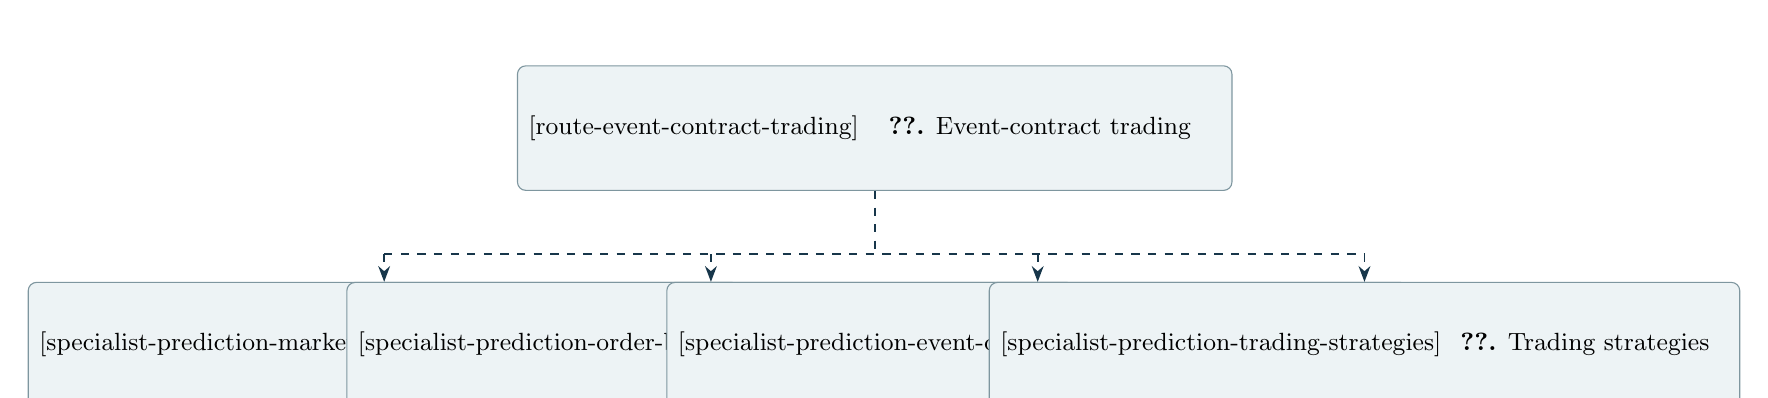
\begin{tikzpicture}[x=1cm,y=1cm]
\node[pathnode] (event-contract-trading) at (6.23,0) {\MeasurePathNode{4.6cm}{\textbf{\ref*{route-event-contract-trading}.} Event-contract trading}\hyperref[route-event-contract-trading]{\parbox[c][\pathnodeheight][c]{4.6cm}{\centering \textbf{\ref*{route-event-contract-trading}.} Event-contract trading}}};
\node[pathnode] (prediction-market-design) at (0.00,-2.75) {\MeasurePathNode{3.65cm}{\textbf{\ref*{specialist-prediction-market-design}.} Automated market makers}\hyperref[specialist-prediction-market-design]{\parbox[c][\pathnodeheight][c]{3.65cm}{\centering \textbf{\ref*{specialist-prediction-market-design}.} Automated market makers}}};
\node[pathnode] (prediction-order-book-mm) at (4.15,-2.75) {\MeasurePathNode{3.65cm}{\textbf{\ref*{specialist-prediction-order-book-mm}.} Order-book market making}\hyperref[specialist-prediction-order-book-mm]{\parbox[c][\pathnodeheight][c]{3.65cm}{\centering \textbf{\ref*{specialist-prediction-order-book-mm}.} Order-book market making}}};
\node[pathnode] (prediction-event-derivatives) at (8.30,-2.75) {\MeasurePathNode{3.65cm}{\textbf{\ref*{specialist-prediction-event-derivatives}.} Event derivatives}\hyperref[specialist-prediction-event-derivatives]{\parbox[c][\pathnodeheight][c]{3.65cm}{\centering \textbf{\ref*{specialist-prediction-event-derivatives}.} Event derivatives}}};
\node[pathnode] (prediction-trading-strategies) at (12.45,-2.75) {\MeasurePathNode{3.65cm}{\textbf{\ref*{specialist-prediction-trading-strategies}.} Trading strategies}\hyperref[specialist-prediction-trading-strategies]{\parbox[c][\pathnodeheight][c]{3.65cm}{\centering \textbf{\ref*{specialist-prediction-trading-strategies}.} Trading strategies}}};
\draw[entryline] (event-contract-trading.south) -- (6.23,-1.60);
\draw[entryline] (0.00,-1.60) -- (12.45,-1.60);
\draw[entryarrow] (0.00,-1.60) -- (prediction-market-design.north);
\draw[entryarrow] (4.15,-1.60) -- (prediction-order-book-mm.north);
\draw[entryarrow] (8.30,-1.60) -- (prediction-event-derivatives.north);
\draw[entryarrow] (12.45,-1.60) -- (prediction-trading-strategies.north);
\end{tikzpicture}\end{center}
\textbf{Bring these foundations with you.}\begin{itemize}
\item \hyperref[route-execution-market-making]{Market microstructure and market making} --- needed by \hyperref[specialist-prediction-order-book-mm]{Order-book market making}.
\item \hyperref[route-volatility-options]{Option pricing, volatility models and hedging} --- needed by \hyperref[specialist-prediction-event-derivatives]{Event derivatives}.
\item \hyperref[specialist-backtest-inference]{Backtest inference, multiple testing and Sharpe-ratio statistics} --- needed by \hyperref[specialist-prediction-trading-strategies]{Trading strategies}.
\end{itemize}\hyperref[learning-map]{Return to the whole-guide DAG.}
\Needspace{12\baselineskip}
\subsection{Automated market makers and scoring rules}\label{specialist-prediction-market-design}
\textbf{Specialist pathway.} In \hyperref[route-event-contract-trading]{Event-contract trading: market making, derivatives and strategies}.

\textbf{Outcome.} Design or evaluate an automated market maker for event contracts: loss bound, liquidity, arbitrage-free pricing across related outcomes, and incentives for strategic traders.

\textbf{Prerequisites.} Event-contract trading: market making, derivatives and strategies; convex optimisation basics.

\textbf{Review first.} \hyperref[route-event-contract-trading]{Event-contract trading: market making, derivatives and strategies}.

\textbf{Required readings, in order}
\begin{enumerate}\raggedright
\Needspace{5\baselineskip}\item \href{institutional_quantitative_finance_reading_list.pdf\#pm-hanson-2003}{Robin Hanson, ``Combinatorial Information Market Design''}\CataloguePage{509}\NoteKey{pm-hanson-2003}\par \textbf{Mechanics.} See why combinatorial outcome spaces need a scoring-rule market maker rather than thin order books.
\Needspace{5\baselineskip}\item \href{institutional_quantitative_finance_reading_list.pdf\#ev-pennock-2004}{David M. Pennock, ``A dynamic pari-mutuel market for hedging, wagering, and information aggregation''}\CataloguePage{510}\NoteKey{ev-pennock-2004}\par \textbf{Mechanics.} Combine a pari-mutuel pool with continuous trading in a dynamic pari-mutuel market.
\Needspace{5\baselineskip}\item \href{institutional_quantitative_finance_reading_list.pdf\#catalogue-0881}{Robin Hanson, ``Logarithmic Market Scoring Rules for Modular Combinatorial Information Aggregation''}\CataloguePage{509}\NoteKey{catalogue-0881}\par \textbf{Valuation.} Derive LMSR prices and the market maker's worst-case loss.
\Needspace{5\baselineskip}\item \href{institutional_quantitative_finance_reading_list.pdf\#ev-dimitrov-sami-2008}{Stanko Dimitrov and Rahul Sami, ``Non-myopic strategies in prediction markets''}\CataloguePage{510}\NoteKey{ev-dimitrov-sami-2008}\par \textbf{Theory.} See why truthful trading under LMSR is only myopically optimal, and how discounting limits bluffing.
\Needspace{5\baselineskip}\item \href{institutional_quantitative_finance_reading_list.pdf\#pm-chen-pennock-2007}{Yiling Chen and David M. Pennock, ``A Utility Framework for Bounded-Loss Market Makers''}\CataloguePage{509}\NoteKey{pm-chen-pennock-2007}\par \textbf{Valuation.} Generalise to bounded-loss market makers derived from a utility function.
\Needspace{5\baselineskip}\item \href{institutional_quantitative_finance_reading_list.pdf\#pm-abernethy-chen-vaughan-2013}{Jacob Abernethy, Yiling Chen and Jennifer Wortman Vaughan, ``Efficient Market Making via Convex Optimization, and a Connection to Online Learning''}\CataloguePage{509}\NoteKey{pm-abernethy-chen-vaughan-2013}\par \textbf{Valuation.} Build cost functions by convex optimisation; trade off loss bound, liquidity and expressiveness.
\Needspace{5\baselineskip}\item \href{institutional_quantitative_finance_reading_list.pdf\#pm-othman-2013}{Abraham Othman, David M. Pennock, Daniel M. Reeves and Tuomas Sandholm, ``A Practical Liquidity-Sensitive Automated Market Maker''}\CataloguePage{509}\NoteKey{pm-othman-2013}\par \textbf{Valuation.} Make liquidity grow with volume, and note what is given up when prices need not sum to one.
\Needspace{5\baselineskip}\item \href{institutional_quantitative_finance_reading_list.pdf\#pm-kroer-2016}{Christian Kroer, Miroslav Dudík, Sébastien Lahaie and Sivaraman Balakrishnan, ``Arbitrage-Free Combinatorial Market Making via Integer Programming''}\CataloguePage{509}\NoteKey{pm-kroer-2016}\par \textbf{Optimization.} Keep prices of logically related outcomes arbitrage-free with integer programming.
\Needspace{5\baselineskip}\item \href{institutional_quantitative_finance_reading_list.pdf\#ev-brahma-2012}{Aseem Brahma, Mithun Chakraborty, Sanmay Das, Allen Lavoie and Malik Magdon-Ismail, ``A bayesian market maker''}\CataloguePage{510}\NoteKey{ev-brahma-2012}\par \textbf{Valuation.} Trade bounded loss for faster learning with a Bayesian market maker.
\Needspace{5\baselineskip}\item \href{institutional_quantitative_finance_reading_list.pdf\#exp-uniform-amm}{Ciamac C. Moallemi, Dan Robinson and Brian Zhu, Uniform-Loss Automated Market Making for Prediction Markets; AFT 2026 proceedings volume}\CataloguePage{510}\NoteKey{exp-uniform-amm}\par \textbf{Valuation.} Design a binary-market AMM whose subsidy loss stays proportional to pool value across price states.
\Needspace{5\baselineskip}\item \href{institutional_quantitative_finance_reading_list.pdf\#w3-amini-prediction-amm}{Hamed Amini, Maxim Bichuch and Zachary Feinstein, ``Decentralized Prediction Markets and Sports Books''}\CataloguePage{510}\NoteKey{w3-amini-prediction-amm}\par \textbf{Valuation.} Compare a liquidity-based AMM design for decentralised prediction markets and sports books.
\end{enumerate}
\Needspace{5\baselineskip}\textbf{Checkpoint.} Implement LMSR, one liquidity-sensitive variant and a Bayesian market maker for a three-outcome event. Simulate informed and noise traders, add a price jump, and report worst-case and realised market-maker loss, price error, recovery time and effective spread against the liquidity parameter. Add a logically related second market and show how an arbitrage-free constraint changes the quotes.

\textbf{Optional branches.} \href{institutional_quantitative_finance_reading_list.pdf\#exp-lvr}{Connect binary-market AMM losses to loss-versus-rebalancing in token AMMs.}\BranchPage{477} \href{institutional_quantitative_finance_reading_list.pdf\#ev-chen-pennock-2010}{Survey the design objectives of prediction mechanisms, including peer prediction.}\BranchPage{510}
\par{\small \hyperref[learning-map]{Learning pathway DAG} \textbar{} \hyperref[route-event-contract-trading]{Section overview} \textbar{} \hyperref[map-event-contract-trading]{Section DAG}\NoteKey{prediction-market-design}}
\Needspace{12\baselineskip}
\subsection{Order-book market making: spreads, adverse selection and who earns}\label{specialist-prediction-order-book-mm}
\textbf{Specialist pathway.} In \hyperref[route-event-contract-trading]{Event-contract trading: market making, derivatives and strategies}.

\textbf{Outcome.} Quote an event-contract order book or answer request-for-quote flow: set fair value, spread and inventory limits, measure adverse selection and know which takers cross-subsidise it.

\textbf{Prerequisites.} Event-contract trading: market making, derivatives and strategies; inventory and adverse-selection models from Market microstructure and market making.

\textbf{Review first.} \hyperref[route-event-contract-trading]{Event-contract trading: market making, derivatives and strategies}; \hyperref[route-execution-market-making]{Market microstructure and market making}.

\textbf{Required readings, in order}
\begin{enumerate}\raggedright
\Needspace{5\baselineskip}\item \href{institutional_quantitative_finance_reading_list.pdf\#ev-kalshi-orderbook-rfq}{Kalshi, Orderbook Responses; Request for Quote (RFQ)}\CataloguePage{512}\NoteKey{ev-kalshi-orderbook-rfq}\par \textbf{Mechanics.} Read a book of YES and NO bids, and the request-for-quote route used for combos.
\Needspace{5\baselineskip}\item \href{institutional_quantitative_finance_reading_list.pdf\#ev-polymarket-market-making}{Polymarket, Market Making; Maker Rebates Program}\CataloguePage{512}\NoteKey{ev-polymarket-market-making}\par \textbf{Mechanics.} Set up two-sided quoting and compute the rebate that adds to the spread.
\Needspace{5\baselineskip}\item \href{institutional_quantitative_finance_reading_list.pdf\#catalogue-0884}{Philipp D. Dubach, ``The Anatomy of a Decentralized Prediction Market: Microstructure Evidence from the Polymarket Order Book''}\CataloguePage{511}\NoteKey{catalogue-0884}\par \textbf{Evidence.} Measure spreads, depth and maker concentration on a hybrid order book; treat public-feed trade direction with care.
\Needspace{5\baselineskip}\item \href{institutional_quantitative_finance_reading_list.pdf\#ev-bartlett-ohara-2026}{Robert Bartlett and Maureen O'Hara, ``Adverse Selection in Prediction Markets: Evidence from Kalshi''}\CataloguePage{511}\NoteKey{ev-bartlett-ohara-2026}\par \textbf{Evidence.} Measure informed price impact and toxicity, and the YES-overbetting that pays for it.
\Needspace{5\baselineskip}\item \href{institutional_quantitative_finance_reading_list.pdf\#pm-ng-peng-tao-zhou-2025}{Hunter Ng, Lin Peng, Yubo Tao and Dexin Zhou, ``Price Discovery and Trading in Modern Prediction Markets''}\CataloguePage{511}\NoteKey{pm-ng-peng-tao-zhou-2025}\par \textbf{Evidence.} Measure cross-venue price discovery and the predictive power of large-trade imbalance.
\Needspace{5\baselineskip}\item \href{institutional_quantitative_finance_reading_list.pdf\#pm-rothschild-sethi-2016}{David Rothschild and Rajiv Sethi, ``Trading Strategies and Market Microstructure: Evidence from a Prediction Market''}\CataloguePage{511}\NoteKey{pm-rothschild-sethi-2016}\par \textbf{Evidence.} Classify trader strategies from account-level data, including a suspected manipulator.
\Needspace{5\baselineskip}\item \href{institutional_quantitative_finance_reading_list.pdf\#pm-gomez-cram-2026}{Roberto Gómez-Cram, Yunhan Guo, Theis Ingerslev Jensen and Howard Kung, ``Prediction Market Accuracy: Crowd Wisdom or Informed Minority?''}\CataloguePage{511}\NoteKey{pm-gomez-cram-2026}\par \textbf{Evidence.} Test whether accuracy comes from the crowd or a persistent informed minority.
\Needspace{5\baselineskip}\item \href{institutional_quantitative_finance_reading_list.pdf\#ev-liu-2026}{Siyang Liu, ``Wisdom of the Crowd or Wisdom of the Insider? Insider Trading on Prediction Markets''}\CataloguePage{507}\NoteKey{ev-liu-2026}\par \textbf{Evidence.} See how much market makers lose in markets compromised by insiders.
\Needspace{5\baselineskip}\item \href{institutional_quantitative_finance_reading_list.pdf\#ev-birge-2021}{John R. Birge, Yifan Feng, N. Bora Keskin and Adam Schultz, ``Dynamic Learning and Market Making in Spread Betting Markets with Informed Bettors''}\CataloguePage{512}\NoteKey{ev-birge-2021}\par \textbf{Theory.} Learn prices without being manipulated by strategic informed bettors.
\end{enumerate}
\Needspace{5\baselineskip}\textbf{Checkpoint.} Build a quoting model for one recurring Kalshi or Polymarket series: fair value from an external forecast, a spread that widens with time to news and inventory, and the venue's fee and rebate. Backtest it on historical trades with queue-position assumptions stated, then split P\&L into spread, rebate, inventory and adverse selection, and compare single-name with broad-based markets.

\textbf{Optional branches.} \href{institutional_quantitative_finance_reading_list.pdf\#ev-levitt-2004}{Contrast a bookmaker who takes positions with a market maker who matches flow.}\BranchPage{501} \href{institutional_quantitative_finance_reading_list.pdf\#ev-shin-1993}{Infer the share of informed flow from quoted spreads.}\BranchPage{506}
\par{\small \hyperref[learning-map]{Learning pathway DAG} \textbar{} \hyperref[route-event-contract-trading]{Section overview} \textbar{} \hyperref[map-event-contract-trading]{Section DAG}\NoteKey{prediction-order-book-mm}}
\Needspace{12\baselineskip}
\subsection{Event derivatives: binary options, parimutuel auctions, combos and belief volatility}\label{specialist-prediction-event-derivatives}
\textbf{Specialist pathway.} In \hyperref[route-event-contract-trading]{Event-contract trading: market making, derivatives and strategies}.

\textbf{Outcome.} Price an event contract as a digital option, extract a distribution from a strike ladder, model the volatility of a probability, and price a combo with correlated legs.

\textbf{Prerequisites.} Event-contract trading: market making, derivatives and strategies; digital-option pricing from the Option pricing, volatility models and hedging overview. Option-implied densities, tail risk and expected returns (11.2) helps with density extraction.

\textbf{Review first.} \hyperref[route-event-contract-trading]{Event-contract trading: market making, derivatives and strategies}; \hyperref[route-volatility-options]{Option pricing, volatility models and hedging}.

\textbf{Required readings, in order}
\begin{enumerate}\raggedright
\Needspace{5\baselineskip}\item \href{institutional_quantitative_finance_reading_list.pdf\#pm-gurkaynak-wolfers-2005}{Refet S. Gürkaynak and Justin Wolfers, ``Macroeconomic Derivatives: An Initial Analysis of Market-Based Macro Forecasts, Uncertainty, and Risk''; NBER working paper}\CataloguePage{512}\NoteKey{pm-gurkaynak-wolfers-2005}\par \textbf{Evidence.} Read market forecasts of macro releases from parimutuel economic-derivative auctions.
\Needspace{5\baselineskip}\item \href{institutional_quantitative_finance_reading_list.pdf\#ev-lange-economides-2005}{Jeffrey Lange and Nicholas Economides, ``A Parimutuel Market Microstructure for Contingent Claims''}\CataloguePage{512}\NoteKey{ev-lange-economides-2005}\par \textbf{Mechanics.} Learn the parimutuel call auction those auctions used.
\Needspace{5\baselineskip}\item \href{institutional_quantitative_finance_reading_list.pdf\#wide-breeden-litzenberger}{Douglas T. Breeden and Robert H. Litzenberger, ``Prices of State-Contingent Claims Implicit in Option Prices''}\CataloguePage{118}\NoteKey{wide-breeden-litzenberger}\par \textbf{Valuation.} Recover state prices from a strip of option prices.
\Needspace{5\baselineskip}\item \href{institutional_quantitative_finance_reading_list.pdf\#ev-lee-lee-lee-2026-crypto}{Seungju Lee, Yebon Lee and Jaewook Lee, ``Cryptocurrency prediction markets through the derivatives lens: Evidence from Kalshi and Polymarket''}\CataloguePage{513}\NoteKey{ev-lee-lee-lee-2026-crypto}\par \textbf{Evidence.} Treat crypto event contracts as digital options: implied volatility, densities and variance premia.
\Needspace{5\baselineskip}\item \href{institutional_quantitative_finance_reading_list.pdf\#ev-goel-2026}{Aditya Goel, ``Measuring macroeconomic surprise magnitude with prediction markets: Market-implied dispersion from Kalshi''}\CataloguePage{513}\NoteKey{ev-goel-2026}\par \textbf{Evidence.} Extract the implied interquartile range of macro releases from Kalshi strike ladders.
\Needspace{5\baselineskip}\item \href{institutional_quantitative_finance_reading_list.pdf\#ev-archak-ipeirotis-2009}{Nikolay Archak and Panagiotis G. Ipeirotis, ``Modeling volatility in prediction markets''}\CataloguePage{513}\NoteKey{ev-archak-ipeirotis-2009}\par \textbf{Valuation.} Derive the volatility of a rational event price from an ability diffusion.
\Needspace{5\baselineskip}\item \href{institutional_quantitative_finance_reading_list.pdf\#ev-dalen-2025}{Shaw Dalen, ``Toward Black--Scholes for Prediction Markets: A Unified Kernel and Market Maker's Handbook''}\CataloguePage{513}\NoteKey{ev-dalen-2025}\par \textbf{Valuation.} Model log-odds as a jump-diffusion and define variance and correlation contracts on probabilities.
\Needspace{5\baselineskip}\item \href{institutional_quantitative_finance_reading_list.pdf\#ev-polymarket-combos}{Polymarket, How Combos Work; Market Makers (Combos)}\CataloguePage{513}\NoteKey{ev-polymarket-combos}\par \textbf{Mechanics.} See how combos are built and quoted by request for quote.
\Needspace{5\baselineskip}\item \href{institutional_quantitative_finance_reading_list.pdf\#ev-moshrefi-2026}{Niusha Moshrefi, ``Prices, Probabilities, and Parlays: Systematic Bias in Sports Prediction Markets''}\CataloguePage{513}\NoteKey{ev-moshrefi-2026}\par \textbf{Evidence.} Measure how far parlays are overpriced relative to their legs.
\end{enumerate}
\Needspace{5\baselineskip}\textbf{Checkpoint.} For one month of Kalshi CPI or bitcoin strike ladders, convert prices into a risk-neutral distribution, compare its width with the realised outcome and a survey or option-implied benchmark, and report coverage. Then fit a logit diffusion with jumps to one contract's price path, and price a two-leg combo under independence and under a stated correlation; compare both with the quoted combo price.

\textbf{Optional branches.} \href{institutional_quantitative_finance_reading_list.pdf\#ev-kalshi-orderbook-rfq}{Read how combo requests reach makers on a regulated exchange.}\BranchPage{512}
\par{\small \hyperref[learning-map]{Learning pathway DAG} \textbar{} \hyperref[route-event-contract-trading]{Section overview} \textbar{} \hyperref[map-event-contract-trading]{Section DAG}\NoteKey{prediction-event-derivatives}}
\Needspace{12\baselineskip}
\subsection{Trading strategies: longshots, arbitrage and stake sizing}\label{specialist-prediction-trading-strategies}
\textbf{Specialist pathway.} In \hyperref[route-event-contract-trading]{Event-contract trading: market making, derivatives and strategies}.

\textbf{Outcome.} Test an event-contract strategy (price-level tilts, model-based value betting or arbitrage across linked contracts) net of fees, capacity and account limits, and size it with fractional Kelly.

\textbf{Prerequisites.} Event-contract trading: market making, derivatives and strategies; Backtest inference, multiple testing and Sharpe-ratio statistics (3.1).

\textbf{Review first.} \hyperref[route-event-contract-trading]{Event-contract trading: market making, derivatives and strategies}; \hyperref[specialist-backtest-inference]{Backtest inference, multiple testing and Sharpe-ratio statistics}.

\textbf{Required readings, in order}
\begin{enumerate}\raggedright
\Needspace{5\baselineskip}\item \href{institutional_quantitative_finance_reading_list.pdf\#ev-hausch-ziemba-rubinstein-1981}{Donald B. Hausch, William T. Ziemba and Mark Rubinstein, ``Efficiency of the Market for Racetrack Betting''}\CataloguePage{500}\NoteKey{ev-hausch-ziemba-rubinstein-1981}\par \textbf{Evidence.} Find positive-expectation place and show bets by comparing model probabilities with pool sizes.
\Needspace{5\baselineskip}\item \href{institutional_quantitative_finance_reading_list.pdf\#w2-thorp-kelly}{Edward O. Thorp, ``The Kelly Criterion in Blackjack, Sports Betting, and the Stock Market''}\CataloguePage{102}\NoteKey{w2-thorp-kelly}\par \textbf{Methods.} Apply the Kelly criterion to betting and investing, with its drawbacks.
\Needspace{5\baselineskip}\item \href{institutional_quantitative_finance_reading_list.pdf\#ev-uhrin-2021}{Matej Uhrín, Gustav Šourek, Ondřej Hubáček and Filip Železný, ``Optimal sports betting strategies in practice: an experimental review''}\CataloguePage{514}\NoteKey{ev-uhrin-2021}\par \textbf{Methods.} Compare Kelly and portfolio betting rules with the risk controls practice needs.
\Needspace{5\baselineskip}\item \href{institutional_quantitative_finance_reading_list.pdf\#ev-cardozo-rivero-2026}{Marcos Cardozo and José Ignacio Rivero-Wildemauwe, ``The Favorite-Longshot Bias in Prediction Markets: Evidence from Polymarket''}\CataloguePage{515}\NoteKey{ev-cardozo-rivero-2026}\par \textbf{Evidence.} Measure returns by price level on Polymarket, and how grouping contracts changes them.
\Needspace{5\baselineskip}\item \href{institutional_quantitative_finance_reading_list.pdf\#ev-berg-rietz-2019}{Joyce E. Berg and Thomas A. Rietz, ``Longshots, overconfidence and efficiency on the Iowa Electronic Market''}\CataloguePage{515}\NoteKey{ev-berg-rietz-2019}\par \textbf{Counter-evidence.} Find no longshot bias on the Iowa markets, and compute Sharpe ratios of simple strategies.
\Needspace{5\baselineskip}\item \href{institutional_quantitative_finance_reading_list.pdf\#pm-moskowitz-2021}{Tobias J. Moskowitz, ``Asset Pricing and Sports Betting''}\CataloguePage{513}\NoteKey{pm-moskowitz-2021}\par \textbf{Evidence.} Test momentum and value in betting lines, where contracts carry no systematic risk.
\Needspace{5\baselineskip}\item \href{institutional_quantitative_finance_reading_list.pdf\#ev-hubacek-sourek-zelezny-2019}{Ondřej Hubáček, Gustav Šourek and Filip Železný, ``Exploiting sports-betting market using machine learning''}\CataloguePage{514}\NoteKey{ev-hubacek-sourek-zelezny-2019}\par \textbf{Methods.} Build a model that disagrees with the bookmaker where it matters, and allocate stakes as a portfolio.
\Needspace{5\baselineskip}\item \href{institutional_quantitative_finance_reading_list.pdf\#ev-kaunitz-zhong-kreiner-2017}{Lisandro Kaunitz, Shenjun Zhong and Javier Kreiner, ``Beating the Bookies with Their Own Numbers---and How the Online Sports Betting Market Is Rigged''}\CataloguePage{514}\NoteKey{ev-kaunitz-zhong-kreiner-2017}\par \textbf{Evidence.} Bet against outlying bookmaker odds, and see the account limits that follow.
\Needspace{5\baselineskip}\item \href{institutional_quantitative_finance_reading_list.pdf\#ev-gebele-mutzel-matthes-2026}{Jonas Gebele, Timm Mutzel and Florian Matthes, ``Executable Arbitrage and Market Efficiency in Prediction Markets''}\CataloguePage{514}\NoteKey{ev-gebele-mutzel-matthes-2026}\par \textbf{Evidence.} Measure realised arbitrage in linked negative-risk markets.
\Needspace{5\baselineskip}\item \href{institutional_quantitative_finance_reading_list.pdf\#ev-cheng-yang-zou-2026}{Guang Cheng, Jiaxin Yang and Haoxuan Zou, ``Arbitrage Analysis in Polymarket NBA Markets''}\CataloguePage{514}\NoteKey{ev-cheng-yang-zou-2026}\par \textbf{Evidence.} Count executable arbitrage in liquid NBA markets and its capacity.
\Needspace{5\baselineskip}\item \href{institutional_quantitative_finance_reading_list.pdf\#ev-lee-lee-lee-2026-sports}{Seungju Lee, Yebon Lee and Jaewook Lee, ``Underreaction, salience, and hot-hand beliefs in sports prediction markets: Evidence from Kalshi NBA and NFL event contracts''}\CataloguePage{500}\NoteKey{ev-lee-lee-lee-2026-sports}\par \textbf{Counter-evidence.} See slow price adjustment that a mean-reversion rule cannot exploit after costs.
\end{enumerate}
\Needspace{5\baselineskip}\textbf{Checkpoint.} Specify one strategy in advance (for example, selling contracts priced below 10 cents in one category, or buying where your model and the price disagree by more than the fee). Backtest it on resolved markets with fees, spreads and realistic fill sizes, grouping related contracts by event. Size positions with full and half Kelly, report growth, drawdown and the number of independent events, and repeat on a later period before claiming an edge.

\textbf{Optional branches.} \href{institutional_quantitative_finance_reading_list.pdf\#s7-maclean}{Go deeper into Kelly theory and practice.}\BranchPage{98} \href{institutional_quantitative_finance_reading_list.pdf\#ev-franck-verbeek-nuesch-2010}{Use exchange prices as the benchmark for bookmaker value bets.}\BranchPage{501}
\par{\small \hyperref[learning-map]{Learning pathway DAG} \textbar{} \hyperref[route-event-contract-trading]{Section overview} \textbar{} \hyperref[map-event-contract-trading]{Section DAG}\NoteKey{prediction-trading-strategies}}
\end{document}
